% Latex header for doxygen 1.8.13
\documentclass[twoside]{article}

% Packages required by doxygen
\usepackage{fixltx2e}
\usepackage{calc}
\usepackage{doxygen}
\usepackage[export]{adjustbox} % also loads graphicx
\usepackage{graphicx}
\usepackage[utf8]{inputenc}
\usepackage{makeidx}
\usepackage{multicol}
\usepackage{multirow}
\PassOptionsToPackage{warn}{textcomp}
\usepackage{textcomp}
\usepackage[nointegrals]{wasysym}
\usepackage[table]{xcolor}

% NLS support packages
\usepackage[french]{babel}

% Font selection
\usepackage[T1]{fontenc}
\usepackage[scaled=.90]{helvet}
\usepackage{courier}
\usepackage{amssymb}
\usepackage{sectsty}
\renewcommand{\familydefault}{\sfdefault}
\allsectionsfont{%
  \fontseries{bc}\selectfont%
  \color{darkgray}%
}
\renewcommand{\DoxyLabelFont}{%
  \fontseries{bc}\selectfont%
  \color{darkgray}%
}
\newcommand{\+}{\discretionary{\mbox{\scriptsize$\hookleftarrow$}}{}{}}

% Page & text layout
\usepackage{geometry}
\geometry{%
  a4paper,%
  top=2cm,%
  bottom=2cm,%
  left=1.2cm,%
  right=1.2cm%
}
\tolerance=750
\hfuzz=15pt
\hbadness=750
\setlength{\emergencystretch}{15pt}
\setlength{\parindent}{0cm}
\setlength{\parskip}{3ex plus 2ex minus 2ex}
\makeatletter
\renewcommand{\paragraph}{%
  \@startsection{paragraph}{4}{0ex}{-1.0ex}{1.0ex}{%
    \normalfont\normalsize\bfseries\SS@parafont%
  }%
}
\renewcommand{\subparagraph}{%
  \@startsection{subparagraph}{5}{0ex}{-1.0ex}{1.0ex}{%
    \normalfont\normalsize\bfseries\SS@subparafont%
  }%
}
\makeatother

% Headers & footers
\usepackage{fancyhdr}
\pagestyle{fancyplain}
\fancyhead[LE]{\fancyplain{}{\bfseries\thepage}}
\fancyhead[CE]{\fancyplain{}{}}
\fancyhead[RE]{\fancyplain{}{\bfseries\leftmark}}
\fancyhead[LO]{\fancyplain{}{\bfseries\rightmark}}
\fancyhead[CO]{\fancyplain{}{}}
\fancyhead[RO]{\fancyplain{}{\bfseries\thepage}}
\fancyfoot[LE]{\fancyplain{}{\bfseries\scriptsize R\+O\+V\textquotesingle{}\+N\+ET 0.\+2}}
\fancyfoot[CE]{\fancyplain{}{}}
\fancyfoot[RE]{\fancyplain{}{\bfseries\scriptsize B\+T\+S S\+N\+I\+R La\+Salle Avignon 2020 }}
\fancyfoot[LO]{\fancyplain{}{\bfseries\scriptsize B\+T\+S S\+N\+I\+R La\+Salle Avignon 2020 }}
\fancyfoot[CO]{\fancyplain{}{}}
\fancyfoot[RO]{\fancyplain{}{\bfseries\scriptsize R\+O\+V\textquotesingle{}\+N\+ET 0.\+2}}
\renewcommand{\footrulewidth}{0.4pt}
\renewcommand{\sectionmark}[1]{%
  \markright{\thesection\ #1}%
}

% Indices & bibliography
\usepackage{natbib}
\usepackage[titles]{tocloft}
\setcounter{tocdepth}{3}
\setcounter{secnumdepth}{5}
\makeindex

% Hyperlinks (required, but should be loaded last)
\usepackage{ifpdf}
\ifpdf
  \usepackage[pdftex,pagebackref=true]{hyperref}
\else
  \usepackage[ps2pdf,pagebackref=true]{hyperref}
\fi
\hypersetup{%
  colorlinks=true,%
  linkcolor=blue,%
  citecolor=blue,%
  unicode%
}

% Custom commands
\newcommand{\clearemptydoublepage}{%
  \newpage{\pagestyle{empty}\cleardoublepage}%
}

\usepackage{caption}
\captionsetup{labelsep=space,justification=centering,font={bf},singlelinecheck=off,skip=4pt,position=top}

%===== C O N T E N T S =====

\begin{document}

% Titlepage & ToC
\hypersetup{pageanchor=false,
             bookmarksnumbered=true,
             pdfencoding=unicode
            }
\pagenumbering{alph}
\begin{titlepage}
\vspace*{7cm}

\begin{center}%
{\LARGE R\+O\+V\textquotesingle{}\+N\+ET}\\
\vspace*{1cm}
{\large version 0.\+2}\\
\vspace*{1cm}
{\large B\+T\+S S\+N\+I\+R La\+Salle Avignon 2020}\\
\end{center}
\end{titlepage}
\pagenumbering{roman}
\tableofcontents
\pagenumbering{arabic}
\hypersetup{pageanchor=true}

%--- Begin generated contents ---
\section{Le projet}
\label{index}\hypertarget{index}{}\hypertarget{index_section_tdm}{}\subsection{Table des matières}\label{index_section_tdm}

\begin{DoxyItemize}
\item \hyperlink{page__r_e_a_d_m_e}{R\+E\+A\+D\+ME}
\item \hyperlink{page_changelog}{Changelog}
\item \hyperlink{page_about}{A propos}
\item \hyperlink{page_licence}{Licence G\+PL}
\end{DoxyItemize}\hypertarget{index_section_infos}{}\subsection{Informations}\label{index_section_infos}
\begin{DoxyAuthor}{Auteur}
Servan Tenaille $<$\href{mailto:servan.tenaille@gmail.com}{\tt servan.\+tenaille@gmail.\+com}$>$ 

Anthony Bonnet $<$\href{mailto:bonnet.anthony0@gmail.com}{\tt bonnet.\+anthony0@gmail.\+com}$>$ 
\end{DoxyAuthor}
\begin{DoxyDate}{Date}
2020 
\end{DoxyDate}
\begin{DoxyVersion}{Version}
0.\+2 
\end{DoxyVersion}
\begin{DoxySeeAlso}{Voir également}
\href{https://svn.riouxsvn.com/rovnet/}{\tt https\+://svn.\+riouxsvn.\+com/rovnet/} 
\end{DoxySeeAlso}

\section{Changelog}
\label{page_changelog}
\Hypertarget{page_changelog}
r192 $\vert$ abonnet $\vert$ 2020-\/04-\/02 17\+:04\+:45 +0200 (jeu. 02 avril 2020) $\vert$ 1 ligne

Réajustement documentation

r191 $\vert$ abonnet $\vert$ 2020-\/04-\/02 16\+:56\+:03 +0200 (jeu. 02 avril 2020) $\vert$ 1 ligne

Réajustement documentation

r190 $\vert$ abonnet $\vert$ 2020-\/04-\/02 16\+:44\+:39 +0200 (jeu. 02 avril 2020) $\vert$ 1 ligne

Suppression éléments non interessant pour le client dans le tag 0.\+1

r189 $\vert$ abonnet $\vert$ 2020-\/04-\/02 16\+:41\+:05 +0200 (jeu. 02 avril 2020) $\vert$ 1 ligne

Création du tag 0.\+1

r188 $\vert$ stenaille $\vert$ 2020-\/04-\/02 16\+:30\+:44 +0200 (jeu. 02 avril 2020) $\vert$ 2 lignes

mise a jour documentation

r187 $\vert$ stenaille $\vert$ 2020-\/04-\/02 16\+:28\+:51 +0200 (jeu. 02 avril 2020) $\vert$ 2 lignes

mise a jour documentation

r186 $\vert$ stenaille $\vert$ 2020-\/04-\/02 16\+:24\+:35 +0200 (jeu. 02 avril 2020) $\vert$ 2 lignes

Correction documentation

r185 $\vert$ stenaille $\vert$ 2020-\/04-\/02 16\+:16\+:57 +0200 (jeu. 02 avril 2020) $\vert$ 2 lignes

correction documentation

r184 $\vert$ stenaille $\vert$ 2020-\/04-\/02 16\+:15\+:42 +0200 (jeu. 02 avril 2020) $\vert$ 2 lignes

Mise a jour documentation

r183 $\vert$ abonnet $\vert$ 2020-\/04-\/02 16\+:11\+:18 +0200 (jeu. 02 avril 2020) $\vert$ 1 ligne

Mis a jour documentation

r182 $\vert$ stenaille $\vert$ 2020-\/04-\/02 16\+:10\+:15 +0200 (jeu. 02 avril 2020) $\vert$ 2 lignes

mise a jour des return

r181 $\vert$ abonnet $\vert$ 2020-\/04-\/02 16\+:08\+:04 +0200 (jeu. 02 avril 2020) $\vert$ 1 ligne

Reéinitialisation de la base de données

r180 $\vert$ stenaille $\vert$ 2020-\/04-\/02 16\+:03\+:01 +0200 (jeu. 02 avril 2020) $\vert$ 2 lignes

Suppression fn du \hyperlink{main_8cpp}{main.\+cpp}

r179 $\vert$ abonnet $\vert$ 2020-\/04-\/02 16\+:01\+:11 +0200 (jeu. 02 avril 2020) $\vert$ 1 ligne

Suppression B\+DD obsolete

r178 $\vert$ stenaille $\vert$ 2020-\/04-\/02 15\+:59\+:19 +0200 (jeu. 02 avril 2020) $\vert$ 2 lignes

Suppression fn de \hyperlink{manette_8h}{manette.\+h}

r177 $\vert$ abonnet $\vert$ 2020-\/04-\/02 15\+:59\+:02 +0200 (jeu. 02 avril 2020) $\vert$ 1 ligne

Suppréssion fichier sql obsolete

r176 $\vert$ stenaille $\vert$ 2020-\/04-\/02 15\+:55\+:25 +0200 (jeu. 02 avril 2020) $\vert$ 2 lignes

Rectification documentation

r175 $\vert$ abonnet $\vert$ 2020-\/04-\/02 15\+:52\+:46 +0200 (jeu. 02 avril 2020) $\vert$ 1 ligne

Mis a jour documentation

r174 $\vert$ stenaille $\vert$ 2020-\/04-\/02 15\+:47\+:03 +0200 (jeu. 02 avril 2020) $\vert$ 2 lignes

retrait des fn dans \hyperlink{rov_8h}{rov.\+h}

r173 $\vert$ abonnet $\vert$ 2020-\/04-\/02 15\+:45\+:09 +0200 (jeu. 02 avril 2020) $\vert$ 1 ligne

Mis a jour documentation

r172 $\vert$ stenaille $\vert$ 2020-\/04-\/01 15\+:57\+:03 +0200 (mer. 01 avril 2020) $\vert$ 2 lignes

Création slot enregister\+Mesure\+B\+D\+D() et signal enregistrer\+Mesures()

r171 $\vert$ abonnet $\vert$ 2020-\/03-\/31 18\+:59\+:11 +0200 (mar. 31 mars 2020) $\vert$ 1 ligne

Modification bug chargement des photos -\/$>$ conteneur informations\+Photos de la méthode charger\+Campagne() doit être vidé pour chaque campagne

r170 $\vert$ tvaira $\vert$ 2020-\/03-\/31 18\+:51\+:35 +0200 (mar. 31 mars 2020) $\vert$ 2 lignes

Déplacement du define S\+A\+N\+S\+\_\+\+D\+E\+T\+E\+C\+T\+I\+ON dans \hyperlink{camera_8h}{camera.\+h}

r169 $\vert$ abonnet $\vert$ 2020-\/03-\/31 18\+:22\+:23 +0200 (mar. 31 mars 2020) $\vert$ 1 ligne

Modification structure \hyperlink{struct_photo}{Photo} -\/$>$ cette dernière ne comprend plus les données issues des capteurs

r168 $\vert$ abonnet $\vert$ 2020-\/03-\/31 18\+:19\+:11 +0200 (mar. 31 mars 2020) $\vert$ 1 ligne

Ajout define S\+A\+N\+S\+\_\+\+D\+E\+T\+E\+C\+T\+I\+ON

r167 $\vert$ abonnet $\vert$ 2020-\/03-\/31 16\+:32\+:35 +0200 (mar. 31 mars 2020) $\vert$ 1 ligne

Modification de l\textquotesingle{}archivage des photos -\/$>$ ces dernières sont enregistré dans la B\+DD directement à la prise

r166 $\vert$ tvaira $\vert$ 2020-\/03-\/30 18\+:24\+:09 +0200 (lun. 30 mars 2020) $\vert$ 2 lignes

Révision de code (voir mail)

r165 $\vert$ stenaille $\vert$ 2020-\/03-\/29 20\+:15\+:03 +0200 (dim. 29 mars 2020) $\vert$ 2 lignes

Ajout suppression image en local et suppression dossier en local

r164 $\vert$ abonnet $\vert$ 2020-\/03-\/29 18\+:55\+:07 +0200 (dim. 29 mars 2020) $\vert$ 1 ligne

Implementation méthode permettant de modifie l\textquotesingle{}etat des bouton de l\textquotesingle{}ihm\+Reglage\+Video

r163 $\vert$ tvaira $\vert$ 2020-\/03-\/29 18\+:53\+:18 +0200 (dim. 29 mars 2020) $\vert$ 2 lignes

Démarrer/\+Arrêter Vidéo

r162 $\vert$ abonnet $\vert$ 2020-\/03-\/29 18\+:18\+:38 +0200 (dim. 29 mars 2020) $\vert$ 1 ligne

Modification \hyperlink{class_i_h_m_reglage_video}{I\+H\+M\+Reglage\+Video} -\/$>$ choix de la camera disponible

r161 $\vert$ abonnet $\vert$ 2020-\/03-\/29 15\+:16\+:10 +0200 (dim. 29 mars 2020) $\vert$ 1 ligne

Création d\textquotesingle{}un dossier du nom de la campagne à la création de cette dernière + enregistrement des photos prise dans ce dossier

r160 $\vert$ abonnet $\vert$ 2020-\/03-\/29 14\+:30\+:09 +0200 (dim. 29 mars 2020) $\vert$ 1 ligne

mis en ordre du code

r159 $\vert$ stenaille $\vert$ 2020-\/03-\/28 18\+:42\+:48 +0100 (sam. 28 mars 2020) $\vert$ 2 lignes

Ajout suppression des photos non voulu lors de l\textquotesingle{}archivage

r158 $\vert$ abonnet $\vert$ 2020-\/03-\/28 18\+:24\+:45 +0100 (sam. 28 mars 2020) $\vert$ 1 ligne

Les photos s\textquotesingle{}enregistresous format P\+NG dans le dossier choisi

r157 $\vert$ abonnet $\vert$ 2020-\/03-\/28 18\+:01\+:12 +0100 (sam. 28 mars 2020) $\vert$ 1 ligne

Modification méthode charger\+Campagne() -\/$>$ prend en compte le nombre de photos presente dans la base de données

r156 $\vert$ abonnet $\vert$ 2020-\/03-\/28 17\+:01\+:35 +0100 (sam. 28 mars 2020) $\vert$ 1 ligne

Modification bug valider\+Campagne

r155 $\vert$ abonnet $\vert$ 2020-\/03-\/28 16\+:27\+:08 +0100 (sam. 28 mars 2020) $\vert$ 1 ligne

Modification structure B\+DD ajout champs chemin\+Sauvegarde à la table campagne

r154 $\vert$ abonnet $\vert$ 2020-\/03-\/28 16\+:02\+:22 +0100 (sam. 28 mars 2020) $\vert$ 1 ligne

Implementation méthode update\+Campagne\+B\+DD

r153 $\vert$ stenaille $\vert$ 2020-\/03-\/28 13\+:58\+:57 +0100 (sam. 28 mars 2020) $\vert$ 2 lignes

Correction bug suppression photo

r152 $\vert$ stenaille $\vert$ 2020-\/03-\/27 18\+:39\+:27 +0100 (ven. 27 mars 2020) $\vert$ 2 lignes

Modification methode supprimer\+Campagne\+B\+DD

r151 $\vert$ stenaille $\vert$ 2020-\/03-\/27 16\+:52\+:34 +0100 (ven. 27 mars 2020) $\vert$ 2 lignes

Modification méthode archiver\+Campagne et supprimer\+Campagne\+B\+DD

r150 $\vert$ stenaille $\vert$ 2020-\/03-\/27 16\+:39\+:43 +0100 (ven. 27 mars 2020) $\vert$ 2 lignes

Ajout méthode Archiver et suppression\+B\+DD

r149 $\vert$ abonnet $\vert$ 2020-\/03-\/27 12\+:57\+:34 +0100 (ven. 27 mars 2020) $\vert$ 1 ligne

Ajout liste des techniciens connus

r148 $\vert$ abonnet $\vert$ 2020-\/03-\/26 18\+:01\+:35 +0100 (jeu. 26 mars 2020) $\vert$ 1 ligne

Modification méthode enregistrer\+Campagne\+B\+DD -\/$>$mise a jour base de données campagnes.\+sqlite

r147 $\vert$ abonnet $\vert$ 2020-\/03-\/26 17\+:40\+:23 +0100 (jeu. 26 mars 2020) $\vert$ 1 ligne

Modification méthode enregistrer\+Campagne\+B\+DD -\/$>$mise a jour base de données campagnes.\+sqlite

r146 $\vert$ abonnet $\vert$ 2020-\/03-\/26 16\+:33\+:25 +0100 (jeu. 26 mars 2020) $\vert$ 1 ligne

Modification methode charger\+Campagnes() -\/$>$ mise a jour base de données campagnes.\+sqlite

r145 $\vert$ stenaille $\vert$ 2020-\/03-\/26 16\+:21\+:16 +0100 (jeu. 26 mars 2020) $\vert$ 1 ligne

Ajout diagramme\+De\+Classe\+Personnel

r144 $\vert$ stenaille $\vert$ 2020-\/03-\/26 15\+:23\+:46 +0100 (jeu. 26 mars 2020) $\vert$ 1 ligne

Ajout diagramme de classe \+: diagramme\+Classe\+Deplacer\+Le\+Robot, diagramme\+Classe\+Piloter\+Le\+Bras, diagramme\+Classe\+Recevoir\+Mesures, diagramme\+Classe\+Visualiser\+Mesures

r143 $\vert$ stenaille $\vert$ 2020-\/03-\/26 14\+:07\+:03 +0100 (jeu. 26 mars 2020) $\vert$ 2 lignes

Modification diagramme cas d\textquotesingle{}utilisation

r142 $\vert$ tvaira $\vert$ 2020-\/03-\/26 13\+:34\+:44 +0100 (jeu. 26 mars 2020) $\vert$ 1 ligne

Modelisation BD

r141 $\vert$ tvaira $\vert$ 2020-\/03-\/25 17\+:25\+:20 +0100 (mer. 25 mars 2020) $\vert$ 1 ligne

Agencement cas utilisation tenaille

r140 $\vert$ stenaille $\vert$ 2020-\/03-\/25 17\+:16\+:37 +0100 (mer. 25 mars 2020) $\vert$ 1 ligne

Ajout diagramme recevoir\+Mesure, visualiser\+Mesures, cas\+Utilisation\+Personnel

r139 $\vert$ abonnet $\vert$ 2020-\/03-\/25 14\+:43\+:19 +0100 (mer. 25 mars 2020) $\vert$ 1 ligne

ajout diagramme de cas d\textquotesingle{}utilisation

r138 $\vert$ abonnet $\vert$ 2020-\/03-\/25 13\+:54\+:22 +0100 (mer. 25 mars 2020) $\vert$ 1 ligne

Modification class \hyperlink{class_i_h_m_creation_campagne}{I\+H\+M\+Creation\+Campagne} -\/$>$ héritage \hyperlink{class_q_dialog}{Q\+Dialog}

r137 $\vert$ abonnet $\vert$ 2020-\/03-\/25 12\+:27\+:45 +0100 (mer. 25 mars 2020) $\vert$ 1 ligne

Rectification diagramme cas d\textquotesingle{}utilisation

r136 $\vert$ tvaira $\vert$ 2020-\/03-\/24 16\+:14\+:45 +0100 (mar. 24 mars 2020) $\vert$ 1 ligne

Maj diagramme de séquence demarrer\+Une\+Campagne

r135 $\vert$ tvaira $\vert$ 2020-\/03-\/24 16\+:13\+:59 +0100 (mar. 24 mars 2020) $\vert$ 2 lignes

Modification classe \hyperlink{class_i_h_m_accueil}{I\+H\+M\+Accueil} en mode modale (type \hyperlink{class_q_dialog}{Q\+Dialog})

r134 $\vert$ abonnet $\vert$ 2020-\/03-\/24 15\+:05\+:30 +0100 (mar. 24 mars 2020) $\vert$ 1 ligne

Ajout diagramme sequence et deploiement

r133 $\vert$ abonnet $\vert$ 2020-\/03-\/24 15\+:03\+:14 +0100 (mar. 24 mars 2020) $\vert$ 1 ligne

modification diagramme deploiement

r132 $\vert$ abonnet $\vert$ 2020-\/03-\/24 13\+:26\+:51 +0100 (mar. 24 mars 2020) $\vert$ 1 ligne

Création diagramme de deploiement

r131 $\vert$ abonnet $\vert$ 2020-\/03-\/24 12\+:47\+:45 +0100 (mar. 24 mars 2020) $\vert$ 1 ligne

Création diagramme sequence piloter\+La\+Camera et demarrerune\+Campagne

r130 $\vert$ tvaira $\vert$ 2020-\/03-\/21 16\+:54\+:23 +0100 (sam. 21 mars 2020) $\vert$ 1 ligne

Validation BD S\+Q\+Lite v1.\+1

r129 $\vert$ abonnet $\vert$ 2020-\/03-\/21 14\+:39\+:48 +0100 (sam. 21 mars 2020) $\vert$ 1 ligne

Modification BD ajout campagne-\/v1.\+1.\+sql

r128 $\vert$ stenaille $\vert$ 2020-\/03-\/20 17\+:46\+:19 +0100 (ven. 20 mars 2020) $\vert$ 1 ligne

ajout .png diagramme piloter\+Le\+Bras

r127 $\vert$ stenaille $\vert$ 2020-\/03-\/20 17\+:45\+:11 +0100 (ven. 20 mars 2020) $\vert$ 1 ligne

Ajout diagramme de sequence piloter le bras

r126 $\vert$ abonnet $\vert$ 2020-\/03-\/20 15\+:41\+:11 +0100 (ven. 20 mars 2020) $\vert$ 1 ligne

Modification BD

r125 $\vert$ abonnet $\vert$ 2020-\/03-\/20 15\+:25\+:48 +0100 (ven. 20 mars 2020) $\vert$ 1 ligne

Modification BD + ajout lieu class \hyperlink{class_campagne}{Campagne}

r124 $\vert$ abonnet $\vert$ 2020-\/03-\/20 15\+:18\+:55 +0100 (ven. 20 mars 2020) $\vert$ 1 ligne

Modification BD + ajout lieu class \hyperlink{class_campagne}{Campagne}

r123 $\vert$ stenaille $\vert$ 2020-\/03-\/20 11\+:13\+:08 +0100 (ven. 20 mars 2020) $\vert$ 1 ligne

Ajout element diagramme de sequence

r122 $\vert$ tvaira $\vert$ 2020-\/03-\/20 07\+:34\+:40 +0100 (ven. 20 mars 2020) $\vert$ 1 ligne

Validation du fichier S\+QL

r121 $\vert$ stenaille $\vert$ 2020-\/03-\/19 19\+:36\+:12 +0100 (jeu. 19 mars 2020) $\vert$ 2 lignes

Ajout du de la fonction archiver\+Campagne

r120 $\vert$ tvaira $\vert$ 2020-\/03-\/19 18\+:40\+:29 +0100 (jeu. 19 mars 2020) $\vert$ 1 ligne

Validation sd deplacer\+Le\+Robot

r119 $\vert$ stenaille $\vert$ 2020-\/03-\/19 18\+:26\+:04 +0100 (jeu. 19 mars 2020) $\vert$ 2 lignes

Mise a jour structure \hyperlink{struct_mesure}{Mesure}

r118 $\vert$ stenaille $\vert$ 2020-\/03-\/19 18\+:23\+:25 +0100 (jeu. 19 mars 2020) $\vert$ 2 lignes

Ajout structure Mesures

r117 $\vert$ abonnet $\vert$ 2020-\/03-\/19 18\+:20\+:23 +0100 (jeu. 19 mars 2020) $\vert$ 1 ligne

Modification B\+DD

r116 $\vert$ abonnet $\vert$ 2020-\/03-\/19 18\+:20\+:05 +0100 (jeu. 19 mars 2020) $\vert$ 1 ligne

Modification B\+DD

r115 $\vert$ abonnet $\vert$ 2020-\/03-\/19 18\+:19\+:37 +0100 (jeu. 19 mars 2020) $\vert$ 1 ligne

Modification B\+DD

r114 $\vert$ stenaille $\vert$ 2020-\/03-\/19 18\+:19\+:09 +0100 (jeu. 19 mars 2020) $\vert$ 1 ligne

Ajout campagnes\+Archives

r113 $\vert$ abonnet $\vert$ 2020-\/03-\/19 18\+:09\+:17 +0100 (jeu. 19 mars 2020) $\vert$ 1 ligne

Ajout fichier campagnes\+En\+Cours-\/v1.\+sql

r112 $\vert$ stenaille $\vert$ 2020-\/03-\/19 18\+:00\+:25 +0100 (jeu. 19 mars 2020) $\vert$ 1 ligne

Ajout de bouml-\/rovnet-\/tenaille

r111 $\vert$ stenaille $\vert$ 2020-\/03-\/19 17\+:59\+:02 +0100 (jeu. 19 mars 2020) $\vert$ 1 ligne

Suppression boulm-\/rovnet-\/tenaille

r110 $\vert$ stenaille $\vert$ 2020-\/03-\/19 17\+:51\+:00 +0100 (jeu. 19 mars 2020) $\vert$ 1 ligne

Ajout des parties manquantes

r109 $\vert$ stenaille $\vert$ 2020-\/03-\/19 17\+:45\+:19 +0100 (jeu. 19 mars 2020) $\vert$ 1 ligne

r108 $\vert$ abonnet $\vert$ 2020-\/03-\/19 17\+:35\+:08 +0100 (jeu. 19 mars 2020) $\vert$ 1 ligne

Modification B\+DD

r107 $\vert$ abonnet $\vert$ 2020-\/03-\/19 17\+:33\+:49 +0100 (jeu. 19 mars 2020) $\vert$ 1 ligne

Modification B\+DD

r106 $\vert$ abonnet $\vert$ 2020-\/03-\/19 17\+:20\+:30 +0100 (jeu. 19 mars 2020) $\vert$ 1 ligne

Modification B\+DD

r105 $\vert$ stenaille $\vert$ 2020-\/03-\/19 17\+:18\+:46 +0100 (jeu. 19 mars 2020) $\vert$ 1 ligne

R\+Ecommit bouml

r104 $\vert$ abonnet $\vert$ 2020-\/03-\/19 17\+:14\+:01 +0100 (jeu. 19 mars 2020) $\vert$ 1 ligne

modification B\+DD

r103 $\vert$ abonnet $\vert$ 2020-\/03-\/19 17\+:07\+:10 +0100 (jeu. 19 mars 2020) $\vert$ 1 ligne

modification B\+DD

r102 $\vert$ abonnet $\vert$ 2020-\/03-\/19 17\+:04\+:58 +0100 (jeu. 19 mars 2020) $\vert$ 1 ligne

Modification B\+DD

r101 $\vert$ abonnet $\vert$ 2020-\/03-\/19 17\+:04\+:21 +0100 (jeu. 19 mars 2020) $\vert$ 1 ligne

Modification B\+DD

r100 $\vert$ tvaira $\vert$ 2020-\/03-\/19 17\+:03\+:48 +0100 (jeu. 19 mars 2020) $\vert$ 1 ligne

Suppression de 2.\+lock

r99 $\vert$ abonnet $\vert$ 2020-\/03-\/19 16\+:54\+:55 +0100 (jeu. 19 mars 2020) $\vert$ 1 ligne

Implémentation méthodes permettant d\textquotesingle{}ajouter une nouvelle campagne dans la B\+DD

r98 $\vert$ abonnet $\vert$ 2020-\/03-\/19 16\+:51\+:14 +0100 (jeu. 19 mars 2020) $\vert$ 1 ligne

modification B\+DD

r97 $\vert$ abonnet $\vert$ 2020-\/03-\/19 16\+:38\+:14 +0100 (jeu. 19 mars 2020) $\vert$ 1 ligne

Deplacement bdd

r96 $\vert$ abonnet $\vert$ 2020-\/03-\/19 16\+:38\+:02 +0100 (jeu. 19 mars 2020) $\vert$ 1 ligne

Deplacement bdd

r95 $\vert$ stenaille $\vert$ 2020-\/03-\/19 16\+:29\+:48 +0100 (jeu. 19 mars 2020) $\vert$ 1 ligne

modification diagramme séquence déplacer le robot format png

r94 $\vert$ stenaille $\vert$ 2020-\/03-\/19 16\+:26\+:18 +0100 (jeu. 19 mars 2020) $\vert$ 1 ligne

diagrame séquence déplacer le robot format png

r93 $\vert$ stenaille $\vert$ 2020-\/03-\/19 16\+:23\+:28 +0100 (jeu. 19 mars 2020) $\vert$ 1 ligne

diagrame séquence déplacer le robot

r92 $\vert$ stenaille $\vert$ 2020-\/03-\/19 16\+:21\+:17 +0100 (jeu. 19 mars 2020) $\vert$ 2 lignes

reglage bug configuration camera

r91 $\vert$ tvaira $\vert$ 2020-\/03-\/19 16\+:19\+:05 +0100 (jeu. 19 mars 2020) $\vert$ 2 lignes

Ajout du déploiement des fichiers S\+Q\+Lite de base

r90 $\vert$ abonnet $\vert$ 2020-\/03-\/19 15\+:54\+:19 +0100 (jeu. 19 mars 2020) $\vert$ 1 ligne

Implémentation méthodes permettant de charger les campagnes présente dans la B\+DD

r89 $\vert$ tvaira $\vert$ 2020-\/03-\/19 08\+:29\+:10 +0100 (jeu. 19 mars 2020) $\vert$ 4 lignes

Ajout des méthodes executer() et recuperer() dans la classe \hyperlink{class_base_de_donnees}{Base\+De\+Donnees} Suppression des warnings

r88 $\vert$ abonnet $\vert$ 2020-\/03-\/18 18\+:01\+:11 +0100 (mer. 18 mars 2020) $\vert$ 1 ligne

Implémentation classe \hyperlink{class_base_de_donnees}{Base\+De\+Donnees}

r87 $\vert$ stenaille $\vert$ 2020-\/03-\/18 17\+:59\+:40 +0100 (mer. 18 mars 2020) $\vert$ 1 ligne

Ajout boulm-\/rovnet-\/tenaille

r86 $\vert$ abonnet $\vert$ 2020-\/03-\/18 17\+:49\+:36 +0100 (mer. 18 mars 2020) $\vert$ 1 ligne

Implémentation classe \hyperlink{class_base_de_donnees}{Base\+De\+Donnees}

r85 $\vert$ stenaille $\vert$ 2020-\/03-\/18 17\+:32\+:44 +0100 (mer. 18 mars 2020) $\vert$ 2 lignes

Ajout campagnes\+Archives

r84 $\vert$ abonnet $\vert$ 2020-\/03-\/18 17\+:28\+:05 +0100 (mer. 18 mars 2020) $\vert$ 1 ligne

Changement nom classe Base\+De\+Donnee -\/$>$ \hyperlink{class_base_de_donnees}{Base\+De\+Donnees}

r83 $\vert$ abonnet $\vert$ 2020-\/03-\/18 17\+:18\+:20 +0100 (mer. 18 mars 2020) $\vert$ 1 ligne

Modification campagne\+En\+Cours -\/$>$ campagnes\+En\+Cours

r82 $\vert$ abonnet $\vert$ 2020-\/03-\/18 16\+:46\+:13 +0100 (mer. 18 mars 2020) $\vert$ 1 ligne

Ajout fichier S\+Q\+Lite campagne\+En\+Cours

r81 $\vert$ abonnet $\vert$ 2020-\/03-\/18 15\+:52\+:18 +0100 (mer. 18 mars 2020) $\vert$ 1 ligne

Realisation sd\+\_\+prendre\+Une\+Photo

r80 $\vert$ stenaille $\vert$ 2020-\/03-\/18 15\+:47\+:56 +0100 (mer. 18 mars 2020) $\vert$ 2 lignes

Ajout de la classe Base\+De\+Donnee

r79 $\vert$ stenaille $\vert$ 2020-\/03-\/18 15\+:04\+:58 +0100 (mer. 18 mars 2020) $\vert$ 2 lignes

Correction warning

r78 $\vert$ abonnet $\vert$ 2020-\/03-\/18 13\+:39\+:32 +0100 (mer. 18 mars 2020) $\vert$ 1 ligne

Ajout diagramme\+Sequence\+Systeme

r77 $\vert$ abonnet $\vert$ 2020-\/03-\/18 13\+:13\+:41 +0100 (mer. 18 mars 2020) $\vert$ 1 ligne

Modification classe album\+Photo -\/$>$ \hyperlink{class_i_h_m_album_photo}{I\+H\+M\+Album\+Photo}

r76 $\vert$ abonnet $\vert$ 2020-\/03-\/17 17\+:26\+:48 +0100 (mar. 17 mars 2020) $\vert$ 1 ligne

Implémentation méthode permettant de garder l\textquotesingle{}etat d\textquotesingle{}une photo lors de la reprise d\textquotesingle{}une campagne

r75 $\vert$ abonnet $\vert$ 2020-\/03-\/17 16\+:14\+:47 +0100 (mar. 17 mars 2020) $\vert$ 1 ligne

Implémentation méthode permettant de garder l\textquotesingle{}etat d\textquotesingle{}une photo lors de la reprise d\textquotesingle{}une campagne

r74 $\vert$ abonnet $\vert$ 2020-\/03-\/17 14\+:21\+:25 +0100 (mar. 17 mars 2020) $\vert$ 1 ligne

Implémentation méthode permettant de changer le status d\textquotesingle{}une photo dans l\textquotesingle{}album photo

r73 $\vert$ tvaira $\vert$ 2020-\/03-\/16 18\+:45\+:45 +0100 (lun. 16 mars 2020) $\vert$ 2 lignes

Exemple Q\+Signal\+Mapper

r72 $\vert$ abonnet $\vert$ 2020-\/03-\/16 17\+:09\+:31 +0100 (lun. 16 mars 2020) $\vert$ 1 ligne

Implémentation méthodes permettant d\textquotesingle{}avoir les informations d\textquotesingle{}une photo dans l\textquotesingle{}album photo

r71 $\vert$ tvaira $\vert$ 2020-\/03-\/16 16\+:32\+:12 +0100 (lun. 16 mars 2020) $\vert$ 2 lignes

Correction erreur erase() campagne\+En\+Cours

r70 $\vert$ abonnet $\vert$ 2020-\/03-\/16 15\+:53\+:30 +0100 (lun. 16 mars 2020) $\vert$ 1 ligne

Implémentation méthodes permettant de supprimer la campagne selectionne

r69 $\vert$ abonnet $\vert$ 2020-\/03-\/16 14\+:56\+:53 +0100 (lun. 16 mars 2020) $\vert$ 1 ligne

Implementation méthodes permettant de reprendre une campagne arreté avec la bonne durée de campagne

r68 $\vert$ abonnet $\vert$ 2020-\/03-\/16 14\+:00\+:20 +0100 (lun. 16 mars 2020) $\vert$ 1 ligne

Ajout d\textquotesingle{}une structure photo + modification de la classe album\+Photo en \hyperlink{class_i_h_m_album_photo}{I\+H\+M\+Album\+Photo}

r67 $\vert$ abonnet $\vert$ 2020-\/03-\/15 17\+:22\+:51 +0100 (dim. 15 mars 2020) $\vert$ 1 ligne

Implementation méthodes permettant de creer une nouvelle campagne

r66 $\vert$ abonnet $\vert$ 2020-\/03-\/14 13\+:50\+:57 +0100 (sam. 14 mars 2020) $\vert$ 1 ligne

Modification sd\+:visualiser environnement

r65 $\vert$ abonnet $\vert$ 2020-\/03-\/14 13\+:50\+:44 +0100 (sam. 14 mars 2020) $\vert$ 1 ligne

Modification sd\+:visualiser environnement

r64 $\vert$ tvaira $\vert$ 2020-\/03-\/14 07\+:52\+:53 +0100 (sam. 14 mars 2020) $\vert$ 1 ligne

Correction sd visualier\+Environnement

r63 $\vert$ tvaira $\vert$ 2020-\/03-\/14 07\+:40\+:33 +0100 (sam. 14 mars 2020) $\vert$ 1 ligne

Ne pas commiter le dossier lock

r62 $\vert$ stenaille $\vert$ 2020-\/03-\/13 20\+:09\+:44 +0100 (ven. 13 mars 2020) $\vert$ 2 lignes

debug chemin image

r61 $\vert$ abonnet $\vert$ 2020-\/03-\/13 19\+:35\+:46 +0100 (ven. 13 mars 2020) $\vert$ 1 ligne

Ajout dossier bouml au projet rovnet

r60 $\vert$ abonnet $\vert$ 2020-\/03-\/13 18\+:10\+:23 +0100 (ven. 13 mars 2020) $\vert$ 1 ligne

Implementation classe \hyperlink{class_i_h_m_accueil}{I\+H\+M\+Accueil}

r59 $\vert$ abonnet $\vert$ 2020-\/03-\/12 15\+:30\+:35 +0100 (jeu. 12 mars 2020) $\vert$ 3 lignes

Implémentation méthodes permettant d\textquotesingle{}envoyer les trames correspondantes au pilotage de la caméra

r58 $\vert$ stenaille $\vert$ 2020-\/03-\/12 12\+:56\+:52 +0100 (jeu. 12 mars 2020) $\vert$ 2 lignes

Ajout Humidité

r57 $\vert$ stenaille $\vert$ 2020-\/03-\/12 12\+:25\+:16 +0100 (jeu. 12 mars 2020) $\vert$ 2 lignes

Documentation

r56 $\vert$ stenaille $\vert$ 2020-\/03-\/12 11\+:53\+:54 +0100 (jeu. 12 mars 2020) $\vert$ 2 lignes

correction bug trame

r55 $\vert$ abonnet $\vert$ 2020-\/03-\/12 11\+:25\+:48 +0100 (jeu. 12 mars 2020) $\vert$ 2 lignes

Modification classe manette -\/$>$ heritage \hyperlink{class_q_gamepad}{Q\+Gamepad}

r54 $\vert$ stenaille $\vert$ 2020-\/03-\/12 10\+:59\+:35 +0100 (jeu. 12 mars 2020) $\vert$ 2 lignes

Ajout structure bouton et modification contruction trame ordre et pince

r53 $\vert$ abonnet $\vert$ 2020-\/03-\/12 10\+:53\+:36 +0100 (jeu. 12 mars 2020) $\vert$ 2 lignes

Mise a jour connect manette

r52 $\vert$ abonnet $\vert$ 2020-\/03-\/12 10\+:26\+:15 +0100 (jeu. 12 mars 2020) $\vert$ 2 lignes

Documentation

r51 $\vert$ stenaille $\vert$ 2020-\/03-\/11 13\+:57\+:06 +0100 (mer. 11 mars 2020) $\vert$ 2 lignes

Mise à jour code

r50 $\vert$ abonnet $\vert$ 2020-\/03-\/11 13\+:37\+:31 +0100 (mer. 11 mars 2020) $\vert$ 1 ligne

Ajustation de la résolution de la caméra

r49 $\vert$ stenaille $\vert$ 2020-\/03-\/11 13\+:36\+:13 +0100 (mer. 11 mars 2020) $\vert$ 2 lignes

Ajout des trames pince

r48 $\vert$ stenaille $\vert$ 2020-\/03-\/11 11\+:00\+:21 +0100 (mer. 11 mars 2020) $\vert$ 2 lignes

optimisation du code sur la partie test des etat de la manette

r47 $\vert$ stenaille $\vert$ 2020-\/03-\/10 22\+:20\+:38 +0100 (mar. 10 mars 2020) $\vert$ 2 lignes

Modification du code (maniere de tester l\textquotesingle{}etat de la manette)

r46 $\vert$ stenaille $\vert$ 2020-\/03-\/10 21\+:40\+:47 +0100 (mar. 10 mars 2020) $\vert$ 2 lignes

Organisation du code

r45 $\vert$ stenaille $\vert$ 2020-\/03-\/10 17\+:05\+:27 +0100 (mar. 10 mars 2020) $\vert$ 2 lignes

Organisation code

r44 $\vert$ tvaira $\vert$ 2020-\/03-\/09 12\+:02\+:19 +0100 (lun. 09 mars 2020) $\vert$ 1 ligne

Revisions de code

r43 $\vert$ abonnet $\vert$ 2020-\/03-\/08 16\+:04\+:13 +0100 (dim. 08 mars 2020) $\vert$ 1 ligne

Modification de la relation rov-\/ihm en relation bidirectionnelle

r42 $\vert$ stenaille $\vert$ 2020-\/03-\/07 18\+:08\+:42 +0100 (sam. 07 mars 2020) $\vert$ 2 lignes

correction code non compilable

r41 $\vert$ abonnet $\vert$ 2020-\/03-\/06 17\+:56\+:17 +0100 (ven. 06 mars 2020) $\vert$ 1 ligne

Mise a jour documentation

r40 $\vert$ stenaille $\vert$ 2020-\/03-\/06 17\+:08\+:45 +0100 (ven. 06 mars 2020) $\vert$ 2 lignes

Ajout des différentes structures \hyperlink{struct_etat_manette_deplacement}{Etat\+Manette\+Deplacement}

r39 $\vert$ stenaille $\vert$ 2020-\/03-\/06 16\+:51\+:30 +0100 (ven. 06 mars 2020) $\vert$ 2 lignes

Modification du code pour correction de bug lors du pilotage du bras

r38 $\vert$ abonnet $\vert$ 2020-\/03-\/06 15\+:12\+:38 +0100 (ven. 06 mars 2020) $\vert$ 1 ligne

Création classe Reglage\+Video et Album\+Photo

r37 $\vert$ tvaira $\vert$ 2020-\/03-\/06 06\+:52\+:47 +0100 (ven. 06 mars 2020) $\vert$ 2 lignes

Test 18.\+04 + define N\+O\+\_\+\+G\+A\+M\+E\+P\+AD pour une utilisation sans manette

r36 $\vert$ stenaille $\vert$ 2020-\/03-\/05 17\+:18\+:36 +0100 (jeu. 05 mars 2020) $\vert$ 2 lignes

modification de la methode creation\+Trame\+Pilotage

r35 $\vert$ abonnet $\vert$ 2020-\/03-\/05 16\+:16\+:42 +0100 (jeu. 05 mars 2020) $\vert$ 1 ligne

Implementation des methodes permettant de capturer plusieurs photos en un campagne et de pouvoir les visualiser clairement

r34 $\vert$ abonnet $\vert$ 2020-\/03-\/05 14\+:14\+:59 +0100 (jeu. 05 mars 2020) $\vert$ 1 ligne

Implementation methodes permettant de capturer une image et de l\textquotesingle{}afficher dans l\textquotesingle{}album photo

r33 $\vert$ stenaille $\vert$ 2020-\/03-\/05 13\+:49\+:38 +0100 (jeu. 05 mars 2020) $\vert$ 2 lignes

Ajout de la création des trames de pilotage

r32 $\vert$ stenaille $\vert$ 2020-\/03-\/04 17\+:05\+:47 +0100 (mer. 04 mars 2020) $\vert$ 2 lignes

Création des connexions et des slots pour les bouton A, B, X, Y

r31 $\vert$ abonnet $\vert$ 2020-\/03-\/04 16\+:46\+:45 +0100 (mer. 04 mars 2020) $\vert$ 1 ligne

Implementation methode permettant d\textquotesingle{}avoir les reglage de la vidéo dans une nouvelle fenetre

r30 $\vert$ stenaille $\vert$ 2020-\/03-\/04 16\+:05\+:29 +0100 (mer. 04 mars 2020) $\vert$ 2 lignes

rectification du code

r29 $\vert$ stenaille $\vert$ 2020-\/03-\/04 15\+:38\+:44 +0100 (mer. 04 mars 2020) $\vert$ 2 lignes

oublie

r28 $\vert$ stenaille $\vert$ 2020-\/03-\/04 15\+:24\+:49 +0100 (mer. 04 mars 2020) $\vert$ 3 lignes

Ajout de l\textquotesingle{}affichage des valeurs températures et radiations de la trame capteur

r27 $\vert$ tvaira $\vert$ 2020-\/03-\/04 14\+:01\+:11 +0100 (mer. 04 mars 2020) $\vert$ 2 lignes

Support pour Open\+CV 2 (Ubuntu 16.\+04) ou 3 (Ubuntu 18.\+04)

r26 $\vert$ abonnet $\vert$ 2020-\/03-\/04 11\+:14\+:21 +0100 (mer. 04 mars 2020) $\vert$ 2 lignes

Suppression label données telemetrie

r25 $\vert$ abonnet $\vert$ 2020-\/03-\/04 10\+:01\+:04 +0100 (mer. 04 mars 2020) $\vert$ 1 ligne

Incrustation telemetrie flux video

r24 $\vert$ abonnet $\vert$ 2020-\/02-\/21 15\+:01\+:22 +0100 (ven. 21 févr. 2020) $\vert$ 1 ligne

Implémentation méthodes permettant une incrustation de l\textquotesingle{}heure et des données télémétriques sur le flux vidéo

r23 $\vert$ stenaille $\vert$ 2020-\/02-\/20 20\+:21\+:15 +0100 (jeu. 20 févr. 2020) $\vert$ 3 lignes

Mise à jour du code (retrait fonction inutile et ajout du code d\textquotesingle{}envoye des trames déplacement)

r22 $\vert$ stenaille $\vert$ 2020-\/02-\/19 18\+:19\+:29 +0100 (mer. 19 févr. 2020) $\vert$ 2 lignes

Modification bug

r21 $\vert$ stenaille $\vert$ 2020-\/02-\/19 18\+:00\+:22 +0100 (mer. 19 févr. 2020) $\vert$ 2 lignes

Modification de la connexion creer\+Trame\+Deplacement

r20 $\vert$ abonnet $\vert$ 2020-\/02-\/19 16\+:48\+:47 +0100 (mer. 19 févr. 2020) $\vert$ 1 ligne

Ajout methode get\+Camera

r19 $\vert$ stenaille $\vert$ 2020-\/02-\/19 16\+:03\+:10 +0100 (mer. 19 févr. 2020) $\vert$ 2 lignes

création de la connexion creer\+Trame\+Deplacement

r18 $\vert$ abonnet $\vert$ 2020-\/02-\/18 13\+:11\+:01 +0100 (mar. 18 févr. 2020) $\vert$ 1 ligne

Implémentation méthodes permettant de modifier les parametres du flux video

r17 $\vert$ stenaille $\vert$ 2020-\/02-\/17 13\+:53\+:38 +0100 (lun. 17 févr. 2020) $\vert$ 2 lignes

suppression du todo des structures

r16 $\vert$ stenaille $\vert$ 2020-\/02-\/17 13\+:52\+:40 +0100 (lun. 17 févr. 2020) $\vert$ 3 lignes

Créations des structures de la manette et ajout des connexion entre la mannette et l\textquotesingle{}application \hyperlink{class_rov}{Rov}

r15 $\vert$ tvaira $\vert$ 2020-\/02-\/15 14\+:24\+:56 +0100 (sam. 15 févr. 2020) $\vert$ 2 lignes

Insertion d\textquotesingle{}un T\+O\+DO pour une structure \hyperlink{class_manette}{Manette}

r14 $\vert$ stenaille $\vert$ 2020-\/02-\/14 17\+:12\+:57 +0100 (ven. 14 févr. 2020) $\vert$ 2 lignes

Todo connexion entre creation\+Trame\+Deplacement et creer\+Trame\+Deplacement

r13 $\vert$ stenaille $\vert$ 2020-\/02-\/14 17\+:03\+:42 +0100 (ven. 14 févr. 2020) $\vert$ 5 lignes

création du signal creation\+Trame\+Deplacement(char deplacement\+AxeX, int puissance, char deplacement\+AxeY) dans la classe manette et la méthode slot creer\+Trame\+Deplacement(char deplacement\+AxeX, int puissance, char deplacement\+AxeY) dans la classe rov

r12 $\vert$ stenaille $\vert$ 2020-\/02-\/14 16\+:48\+:16 +0100 (ven. 14 févr. 2020) $\vert$ 2 lignes

Ajout documentation classe manette

r11 $\vert$ stenaille $\vert$ 2020-\/02-\/14 16\+:33\+:36 +0100 (ven. 14 févr. 2020) $\vert$ 2 lignes

Amélioration du code de la fonction creer\+Trame\+Deplacement()

r10 $\vert$ abonnet $\vert$ 2020-\/02-\/14 15\+:58\+:20 +0100 (ven. 14 févr. 2020) $\vert$ 3 lignes

Implémentation des méthodes permettant de décoder la trame de télémtrie et afficher les données correspondantes

r9 $\vert$ stenaille $\vert$ 2020-\/02-\/14 15\+:50\+:55 +0100 (ven. 14 févr. 2020) $\vert$ 2 lignes

Documentation

r8 $\vert$ stenaille $\vert$ 2020-\/02-\/14 14\+:30\+:28 +0100 (ven. 14 févr. 2020) $\vert$ 2 lignes

ajout class manette

r7 $\vert$ stenaille $\vert$ 2020-\/02-\/14 14\+:27\+:25 +0100 (ven. 14 févr. 2020) $\vert$ 2 lignes

Ajout de la methode detecter\+Manette()

r6 $\vert$ abonnet $\vert$ 2020-\/02-\/14 13\+:50\+:04 +0100 (ven. 14 févr. 2020) $\vert$ 2 lignes

Implémentation des méthodes permmettant d\textquotesingle{}afficher le flux vidéo sur l\textquotesingle{}I\+HM

r5 $\vert$ abonnet $\vert$ 2020-\/02-\/13 16\+:18\+:17 +0100 (jeu. 13 févr. 2020) $\vert$ 1 ligne

r4 $\vert$ abonnet $\vert$ 2020-\/02-\/13 16\+:17\+:44 +0100 (jeu. 13 févr. 2020) $\vert$ 2 lignes

Ajout des attribut de la caméra

r3 $\vert$ abonnet $\vert$ 2020-\/02-\/13 13\+:33\+:24 +0100 (jeu. 13 févr. 2020) $\vert$ 2 lignes

Ajout des classes camera et rov

r2 $\vert$ abonnet $\vert$ 2020-\/02-\/12 14\+:28\+:56 +0100 (mer. 12 févr. 2020) $\vert$ 2 lignes

Création du projet Qt

r1 $\vert$ www-\/data $\vert$ 2020-\/02-\/01 15\+:03\+:29 +0100 (sam. 01 févr. 2020) $\vert$ 1 ligne

Creating initial repository structure 
\section{R\+E\+A\+D\+ME}
\label{page__r_e_a_d_m_e}
\Hypertarget{page__r_e_a_d_m_e}
\hypertarget{page__r_e_a_d_m_e_projet}{}\subsection{Projet}\label{page__r_e_a_d_m_e_projet}
\hypertarget{page__r_e_a_d_m_e_presentation}{}\subsubsection{Présentation}\label{page__r_e_a_d_m_e_presentation}
Les objectifs du projet R\+OV\textquotesingle{}N\+ET sont de se déplacer dans un milieu contaminé afin de faire des prises de vues \+:


\begin{DoxyItemize}
\item Le déplacement se fera à partir d\textquotesingle{}un châssis en liaison filaire​ à 4 roues motorisées indépendamment.
\item Le R\+OV sera équipé \+:
\begin{DoxyItemize}
\item d\textquotesingle{}une caméra d\textquotesingle{}aide au déplacements et/ou de capteurs d\textquotesingle{}obstacles
\item d\textquotesingle{}un capteur de température et de radioactivité
\item d\textquotesingle{}un dispositif de prise de vue motorisé
\item d\textquotesingle{}un bras de robotique avec pince de préhension
\end{DoxyItemize}
\end{DoxyItemize}\hypertarget{page__r_e_a_d_m_e_bdd}{}\subsubsection{Base de données S\+Q\+Lite}\label{page__r_e_a_d_m_e_bdd}



\begin{DoxyCode}
PRAGMA foreign\_keys = ON;

--
-- Structure de la table `campagne`
--

CREATE TABLE IF NOT EXISTS `campagne` (
    `IdCampagne`    INTEGER PRIMARY KEY AUTOINCREMENT,
    `IdTechnicien`  INTEGER NOT NULL,
    `nom`   TEXT NOT NULL UNIQUE,
    `lieu`  TEXT NOT NULL,
    `cheminSauvegarde`  TEXT NOT NULL,
    `date`  DATETIME NOT NULL,
    `duree` INTEGER NOT NULL,
    `enCours` NUMERIC NOT NULL,
    UNIQUE(`IdCampagne`, `IdTechnicien`),
    FOREIGN KEY(IdTechnicien) REFERENCES technicien(IdTechnicien)
);

--
-- Structure de la table `mesure`
--

CREATE TABLE IF NOT EXISTS `mesure` (
    `IdMesure`  INTEGER PRIMARY KEY AUTOINCREMENT,
    `IdCampagne`    INTEGER NOT NULL,
    `heure` DATETIME NOT NULL,
    `temperature`   REAL NOT NULL,
    `radiation` REAL NOT NULL,
    `humidite`  REAL NOT NULL,  
    UNIQUE(`IdMesure`, `IdCampagne`),
    FOREIGN KEY(IdCampagne) REFERENCES campagne(IdCampagne)
);

--
-- Structure de la table `photo`
--

CREATE TABLE IF NOT EXISTS `photo` (
    `IdPhoto`   INTEGER PRIMARY KEY AUTOINCREMENT,
    `IdCampagne`    INTEGER NOT NULL,
    `cheminImage`   TEXT NOT NULL,
    `aGarder`   NUMERIC NOT NULL,
    UNIQUE(`IdPhoto`, `IdCampagne`),
    FOREIGN KEY(IdCampagne) REFERENCES campagne(IdCampagne) 
);

--
-- Structure de la table `technicien`
--

CREATE TABLE IF NOT EXISTS `technicien` (
    `IdTechnicien`  INTEGER PRIMARY KEY AUTOINCREMENT,
    `nom`   TEXT NOT NULL,
    `prenom`    TEXT NOT NULL
);
\end{DoxyCode}
\hypertarget{page__r_e_a_d_m_e_recette}{}\subsubsection{Recette}\label{page__r_e_a_d_m_e_recette}

\begin{DoxyItemize}
\item Servan Tenaille
\begin{DoxyItemize}
\item Prendre en charge une manette par le logiciel
\item Recevoir et Visualiser les mesures des capteurs de température et d\textquotesingle{}irradiation
\item Déplacer le robot
\item Piloter le bras articulé
\item Envoyer les ordres de déplacement au robot et au bras
\item Archiver les mesures
\end{DoxyItemize}
\item Anthony Bonnet
\begin{DoxyItemize}
\item Démarrer une campagne
\item Visualiser l\textquotesingle{}environnement (le flux vidéo de la caméra et les données de télémétrie)
\item Recevoir les données de télémétrie
\item Prendre une photo
\item Configurer le contrôle de la caméra
\item Archiver les photos
\end{DoxyItemize}
\end{DoxyItemize}\hypertarget{page__r_e_a_d_m_e_informations}{}\subsubsection{Informations}\label{page__r_e_a_d_m_e_informations}
\begin{DoxyAuthor}{Auteur}
Servan Tenaille $<$\href{mailto:servan.tenaille@gmail.com}{\tt servan.\+tenaille@gmail.\+com}$>$ 

Anthony Bonnet $<$\href{mailto:bonnet.anthony0@gmail.com}{\tt bonnet.\+anthony0@gmail.\+com}$>$ 
\end{DoxyAuthor}
\begin{DoxyDate}{Date}
2020 
\end{DoxyDate}
\begin{DoxyVersion}{Version}
0.\+2 
\end{DoxyVersion}
\begin{DoxySeeAlso}{Voir également}
\href{https://svn.riouxsvn.com/rovnet/}{\tt https\+://svn.\+riouxsvn.\+com/rovnet/} 
\end{DoxySeeAlso}

\section{A propos}
\label{page_about}
\Hypertarget{page_about}
\begin{DoxyAuthor}{Auteur}
Servan Tenaille $<$\href{mailto:servan.tenaille@gmail.com}{\tt servan.\+tenaille@gmail.\+com}$>$ 

Anthony Bonnet $<$\href{mailto:bonnet.anthony0@gmail.com}{\tt bonnet.\+anthony0@gmail.\+com}$>$ 
\end{DoxyAuthor}
\begin{DoxyDate}{Date}
2020 
\end{DoxyDate}
\begin{DoxyVersion}{Version}
0.\+2 
\end{DoxyVersion}
\begin{DoxySeeAlso}{Voir également}
\href{https://svn.riouxsvn.com/rovnet/}{\tt https\+://svn.\+riouxsvn.\+com/rovnet/} 
\end{DoxySeeAlso}

\section{Licence G\+PL}
\label{page_licence}
\Hypertarget{page_licence}
This program is free software; you can redistribute it and/or modify it under the terms of the G\+NU General Public License as published by the Free Software Foundation; either version 2 of the License, or (at your option) any later version.

This program is distributed in the hope that it will be useful, but W\+I\+T\+H\+O\+UT A\+NY W\+A\+R\+R\+A\+N\+TY; without even the implied warranty of M\+E\+R\+C\+H\+A\+N\+T\+A\+B\+I\+L\+I\+TY or F\+I\+T\+N\+E\+SS F\+OR A P\+A\+R\+T\+I\+C\+U\+L\+AR P\+U\+R\+P\+O\+SE. See the G\+NU General Public License for more details.

You should have received a copy of the G\+NU General Public License along with this program; if not, write to the Free Software Foundation, Inc., 59 Temple Place, Suite 330, Boston, MA 02111-\/1307 U\+SA 
\section{Liste des choses à faire}
\label{todo}
\Hypertarget{todo}

\begin{DoxyRefList}
\item[\label{todo__todo000001}%
\Hypertarget{todo__todo000001}%
Membre \hyperlink{class_i_h_m_rov_a58ba3661c111c9ab2d6f1e3c52f4ec21}{I\+H\+M\+Rov\+:\+:actualiser\+Informations} (Q\+Pixmap \&image)]Tenir compte de la résolution de l\textquotesingle{}image 
\end{DoxyRefList}
\section{Documentation des classes}
\hypertarget{class_base_de_donnees}{}\subsection{Référence de la classe Base\+De\+Donnees}
\label{class_base_de_donnees}\index{Base\+De\+Donnees@{Base\+De\+Donnees}}


Class permettant de s\textquotesingle{}interfacer avec la base de données.  




{\ttfamily \#include \char`\"{}basededonnees.\+h\char`\"{}}



Graphe de collaboration de Base\+De\+Donnees\+:
\nopagebreak
\begin{figure}[H]
\begin{center}
\leavevmode
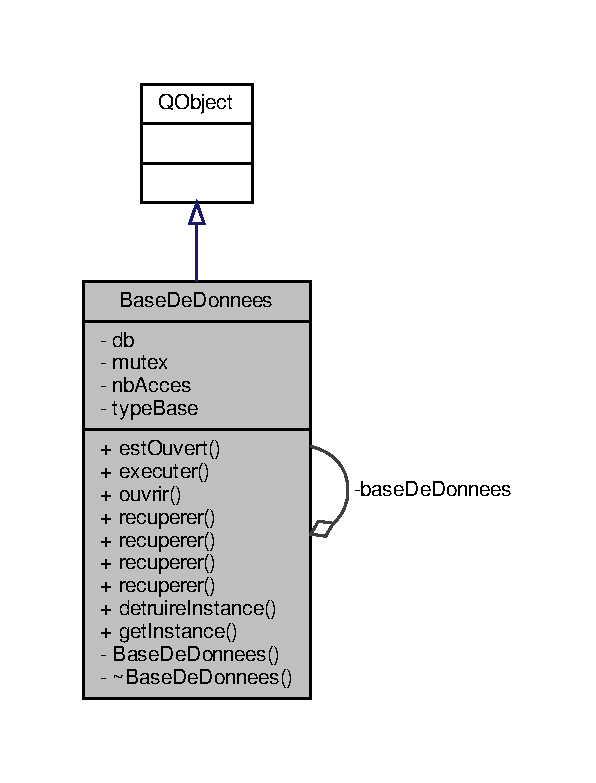
\includegraphics[width=286pt]{class_base_de_donnees__coll__graph}
\end{center}
\end{figure}
\subsubsection*{Fonctions membres publiques}
\begin{DoxyCompactItemize}
\item 
bool \hyperlink{class_base_de_donnees_af9ac332082ffd0dd35e412cefabe5e9c}{est\+Ouvert} ()
\begin{DoxyCompactList}\small\item\em Permet de savoir si la base de données est ouverte ou non. \end{DoxyCompactList}\item 
bool \hyperlink{class_base_de_donnees_aa8de5f8f8bb17edc43f5c0ee33712081}{executer} (Q\+String requete)
\begin{DoxyCompactList}\small\item\em Permet d\textquotesingle{}executer la requete passé en paramètre au format S\+QL. \end{DoxyCompactList}\item 
bool \hyperlink{class_base_de_donnees_a7f6a5510b08017b0d99115a84252f186}{ouvrir} (Q\+String fichier\+Base)
\begin{DoxyCompactList}\small\item\em Permet d\textquotesingle{}ouvrir le fichier de base de données passé en paramètre. \end{DoxyCompactList}\item 
bool \hyperlink{class_base_de_donnees_a77539baad389f5acf754cd2cd452403e}{recuperer} (Q\+String requete, Q\+String \&donnees)
\begin{DoxyCompactList}\small\item\em Permet d\textquotesingle{}executer la requete passé en paramètre au format S\+QL, et remplit le Q\+String de sa réponse. Cette requête permet de récuperer un champs d\textquotesingle{}un enregistrement. \end{DoxyCompactList}\item 
bool \hyperlink{class_base_de_donnees_a2a5c461fa11d404810ae3ebe035d5190}{recuperer} (Q\+String requete, Q\+String\+List \&donnees)
\begin{DoxyCompactList}\small\item\em Permet d\textquotesingle{}executer la requete passé en paramètre au format S\+QL, et remplit le Q\+String\+Liste de sa réponse. Cette requête permet de récuperer plusieurs champs d\textquotesingle{}un enregistrement. \end{DoxyCompactList}\item 
bool \hyperlink{class_base_de_donnees_af9a76eb2b12df784280c379a4b22af62}{recuperer} (Q\+String requete, Q\+Vector$<$ Q\+String $>$ \&donnees)
\begin{DoxyCompactList}\small\item\em Permet d\textquotesingle{}executer la requete passé en paramètre au format S\+QL, et remplit le Q\+Vector$<$\+Q\+String$>$ de sa réponse. Cette requête permet de récuperer un champs de plusieurs enregistrements. \end{DoxyCompactList}\item 
bool \hyperlink{class_base_de_donnees_a68dd0d62ba03b9e8e5aa759d0666cb59}{recuperer} (Q\+String requete, Q\+Vector$<$ Q\+String\+List $>$ \&donnees)
\begin{DoxyCompactList}\small\item\em Permet d\textquotesingle{}executer la requete passé en paramètre au format S\+QL, et remplit le Q\+Vector$<$\+Q\+String\+List$>$ de sa réponse. Cette requête permet de récuperer plusieurs champs de plusieurs enregistrements. \end{DoxyCompactList}\end{DoxyCompactItemize}
\subsubsection*{Fonctions membres publiques statiques}
\begin{DoxyCompactItemize}
\item 
static void \hyperlink{class_base_de_donnees_a457401c0816b888c77ce915997545f4e}{detruire\+Instance} ()
\begin{DoxyCompactList}\small\item\em Permet de detruire l\textquotesingle{}instance en cours, Static elle est accessible depuis n\textquotesingle{}importe où \end{DoxyCompactList}\item 
static \hyperlink{class_base_de_donnees}{Base\+De\+Donnees} $\ast$ \hyperlink{class_base_de_donnees_a58beb2f702f75b257e2e55e25d9f979b}{get\+Instance} (Q\+String type=\char`\"{}Q\+S\+Q\+L\+I\+TE\char`\"{})
\begin{DoxyCompactList}\small\item\em Permet de créer une instance de B\+DD ou de récuperer celle deja en cours, cette méthode controle l\textquotesingle{}instanciation des objet \hyperlink{class_base_de_donnees}{Base\+De\+Donnees}. Static elle est accessible depuis n\textquotesingle{}importe où \end{DoxyCompactList}\end{DoxyCompactItemize}
\subsubsection*{Fonctions membres privées}
\begin{DoxyCompactItemize}
\item 
\hyperlink{class_base_de_donnees_a10dd177f1008f675ab78c2221b2a6750}{Base\+De\+Donnees} (Q\+String type)
\begin{DoxyCompactList}\small\item\em Constructeur de la classe \hyperlink{class_base_de_donnees}{Base\+De\+Donnees} en privé afin de controller ses appels. \end{DoxyCompactList}\item 
\hyperlink{class_base_de_donnees_a5dc474cdbe003644fb0ca7b8f2ec6b93}{$\sim$\+Base\+De\+Donnees} ()
\begin{DoxyCompactList}\small\item\em Destructeur de la classe \hyperlink{class_base_de_donnees}{Base\+De\+Donnees}. \end{DoxyCompactList}\end{DoxyCompactItemize}
\subsubsection*{Attributs privés}
\begin{DoxyCompactItemize}
\item 
Q\+Sql\+Database \hyperlink{class_base_de_donnees_a3e738dcf443370c46a541677ab619f06}{db}
\begin{DoxyCompactList}\small\item\em Objet de type Q\+Sql\+Database permettant la connexion avec la base de données. \end{DoxyCompactList}\item 
Q\+Mutex \hyperlink{class_base_de_donnees_aa1b4696fac87a740f914aa73739086f2}{mutex}
\begin{DoxyCompactList}\small\item\em Objet de type Q\+Mutex permettant de protéger l\textquotesingle{}objet db, en autorisant son accès par un seul thread à la fois. \end{DoxyCompactList}\end{DoxyCompactItemize}
\subsubsection*{Attributs privés statiques}
\begin{DoxyCompactItemize}
\item 
static \hyperlink{class_base_de_donnees}{Base\+De\+Donnees} $\ast$ \hyperlink{class_base_de_donnees_a822ba0b7cf85b1e48ced8efd3d65e266}{base\+De\+Donnees} = nullptr
\begin{DoxyCompactList}\small\item\em Objet de type \hyperlink{class_base_de_donnees}{Base\+De\+Donnees} accessible uniquement depuis une méthode static. \end{DoxyCompactList}\item 
static int \hyperlink{class_base_de_donnees_a5099ecb2922bb31d84cd5d4505298a29}{nb\+Acces} = 0
\begin{DoxyCompactList}\small\item\em Attribut de type int contenant le nombre d\textquotesingle{}accès en cours à la base de données. \end{DoxyCompactList}\item 
static Q\+String \hyperlink{class_base_de_donnees_ab682b82167f494496a6531bfe522b42b}{type\+Base} = \char`\"{}Q\+S\+Q\+L\+I\+TE\char`\"{}
\begin{DoxyCompactList}\small\item\em Attribut de type Q\+String contenant le type de la base de données (My\+S\+QL, S\+Q\+Lite, ...) \end{DoxyCompactList}\end{DoxyCompactItemize}


\subsubsection{Description détaillée}
Class permettant de s\textquotesingle{}interfacer avec la base de données. 

Définition à la ligne \hyperlink{basededonnees_8h_source_l00023}{23} du fichier \hyperlink{basededonnees_8h_source}{basededonnees.\+h}.



\subsubsection{Documentation des constructeurs et destructeur}
\mbox{\Hypertarget{class_base_de_donnees_a10dd177f1008f675ab78c2221b2a6750}\label{class_base_de_donnees_a10dd177f1008f675ab78c2221b2a6750}} 
\index{Base\+De\+Donnees@{Base\+De\+Donnees}!Base\+De\+Donnees@{Base\+De\+Donnees}}
\index{Base\+De\+Donnees@{Base\+De\+Donnees}!Base\+De\+Donnees@{Base\+De\+Donnees}}
\paragraph{\texorpdfstring{Base\+De\+Donnees()}{BaseDeDonnees()}}
{\footnotesize\ttfamily Base\+De\+Donnees\+::\+Base\+De\+Donnees (\begin{DoxyParamCaption}\item[{Q\+String}]{type }\end{DoxyParamCaption})\hspace{0.3cm}{\ttfamily [private]}}



Constructeur de la classe \hyperlink{class_base_de_donnees}{Base\+De\+Donnees} en privé afin de controller ses appels. 


\begin{DoxyParams}{Paramètres}
{\em type} & \\
\hline
\end{DoxyParams}


Définition à la ligne \hyperlink{basededonnees_8cpp_source_l00015}{15} du fichier \hyperlink{basededonnees_8cpp_source}{basededonnees.\+cpp}.



Références \hyperlink{basededonnees_8h_source_l00030}{db}, et \hyperlink{basededonnees_8h_source_l00028}{type\+Base}.



Référencé par \hyperlink{basededonnees_8cpp_source_l00031}{get\+Instance()}.


\begin{DoxyCode}
00016 \{
00017 \textcolor{preprocessor}{    #ifdef DEBUG\_BASEDEDONNEES}
00018     qDebug() << Q\_FUNC\_INFO << type;
00019 \textcolor{preprocessor}{    #endif}
00020     \hyperlink{class_base_de_donnees_a3e738dcf443370c46a541677ab619f06}{db} = QSqlDatabase::addDatabase(type);
00021     \hyperlink{class_base_de_donnees_ab682b82167f494496a6531bfe522b42b}{typeBase} = type;
00022 \}
\end{DoxyCode}
\mbox{\Hypertarget{class_base_de_donnees_a5dc474cdbe003644fb0ca7b8f2ec6b93}\label{class_base_de_donnees_a5dc474cdbe003644fb0ca7b8f2ec6b93}} 
\index{Base\+De\+Donnees@{Base\+De\+Donnees}!````~Base\+De\+Donnees@{$\sim$\+Base\+De\+Donnees}}
\index{````~Base\+De\+Donnees@{$\sim$\+Base\+De\+Donnees}!Base\+De\+Donnees@{Base\+De\+Donnees}}
\paragraph{\texorpdfstring{$\sim$\+Base\+De\+Donnees()}{~BaseDeDonnees()}}
{\footnotesize\ttfamily Base\+De\+Donnees\+::$\sim$\+Base\+De\+Donnees (\begin{DoxyParamCaption}{ }\end{DoxyParamCaption})\hspace{0.3cm}{\ttfamily [private]}}



Destructeur de la classe \hyperlink{class_base_de_donnees}{Base\+De\+Donnees}. 



Définition à la ligne \hyperlink{basededonnees_8cpp_source_l00024}{24} du fichier \hyperlink{basededonnees_8cpp_source}{basededonnees.\+cpp}.


\begin{DoxyCode}
00025 \{
00026 \textcolor{preprocessor}{    #ifdef DEBUG\_BASEDEDONNEES}
00027     qDebug() << Q\_FUNC\_INFO;
00028 \textcolor{preprocessor}{    #endif}
00029 \}
\end{DoxyCode}


\subsubsection{Documentation des fonctions membres}
\mbox{\Hypertarget{class_base_de_donnees_a457401c0816b888c77ce915997545f4e}\label{class_base_de_donnees_a457401c0816b888c77ce915997545f4e}} 
\index{Base\+De\+Donnees@{Base\+De\+Donnees}!detruire\+Instance@{detruire\+Instance}}
\index{detruire\+Instance@{detruire\+Instance}!Base\+De\+Donnees@{Base\+De\+Donnees}}
\paragraph{\texorpdfstring{detruire\+Instance()}{detruireInstance()}}
{\footnotesize\ttfamily void Base\+De\+Donnees\+::detruire\+Instance (\begin{DoxyParamCaption}{ }\end{DoxyParamCaption})\hspace{0.3cm}{\ttfamily [static]}}



Permet de detruire l\textquotesingle{}instance en cours, Static elle est accessible depuis n\textquotesingle{}importe où 



Définition à la ligne \hyperlink{basededonnees_8cpp_source_l00044}{44} du fichier \hyperlink{basededonnees_8cpp_source}{basededonnees.\+cpp}.



Références \hyperlink{basededonnees_8h_source_l00027}{base\+De\+Donnees}, et \hyperlink{basededonnees_8h_source_l00029}{nb\+Acces}.



Référencé par \hyperlink{ihmaccueil_8cpp_source_l00031}{I\+H\+M\+Accueil\+::$\sim$\+I\+H\+M\+Accueil()}.


\begin{DoxyCode}
00045 \{
00046     \textcolor{keywordflow}{if}(\hyperlink{class_base_de_donnees_a822ba0b7cf85b1e48ced8efd3d65e266}{baseDeDonnees} != \textcolor{keyword}{nullptr})
00047     \{
00048         \textcolor{keywordflow}{if}(\hyperlink{class_base_de_donnees_a5099ecb2922bb31d84cd5d4505298a29}{nbAcces} > 0)
00049             \hyperlink{class_base_de_donnees_a5099ecb2922bb31d84cd5d4505298a29}{nbAcces}--;
00050 
00051 \textcolor{preprocessor}{        #ifdef DEBUG\_BASEDEDONNEES}
00052         qDebug() << Q\_FUNC\_INFO << \textcolor{stringliteral}{"nbAcces restants"} << \hyperlink{class_base_de_donnees_a5099ecb2922bb31d84cd5d4505298a29}{nbAcces};
00053 \textcolor{preprocessor}{        #endif}
00054 
00055         \textcolor{keywordflow}{if}(nbAcces == 0)
00056         \{
00057             \textcolor{keyword}{delete} \hyperlink{class_base_de_donnees_a822ba0b7cf85b1e48ced8efd3d65e266}{baseDeDonnees};
00058             \hyperlink{class_base_de_donnees_a822ba0b7cf85b1e48ced8efd3d65e266}{baseDeDonnees} = \textcolor{keyword}{nullptr};
00059         \}
00060     \}
00061 \}
\end{DoxyCode}
\mbox{\Hypertarget{class_base_de_donnees_af9ac332082ffd0dd35e412cefabe5e9c}\label{class_base_de_donnees_af9ac332082ffd0dd35e412cefabe5e9c}} 
\index{Base\+De\+Donnees@{Base\+De\+Donnees}!est\+Ouvert@{est\+Ouvert}}
\index{est\+Ouvert@{est\+Ouvert}!Base\+De\+Donnees@{Base\+De\+Donnees}}
\paragraph{\texorpdfstring{est\+Ouvert()}{estOuvert()}}
{\footnotesize\ttfamily bool Base\+De\+Donnees\+::est\+Ouvert (\begin{DoxyParamCaption}{ }\end{DoxyParamCaption})}



Permet de savoir si la base de données est ouverte ou non. 

\begin{DoxyReturn}{Renvoie}
un booleen correspondant à l\textquotesingle{}état d\textquotesingle{}ouverture de la base de données 
\end{DoxyReturn}


Définition à la ligne \hyperlink{basededonnees_8cpp_source_l00098}{98} du fichier \hyperlink{basededonnees_8cpp_source}{basededonnees.\+cpp}.



Références \hyperlink{basededonnees_8h_source_l00030}{db}, et \hyperlink{basededonnees_8h_source_l00031}{mutex}.


\begin{DoxyCode}
00099 \{
00100     QMutexLocker verrou(&\hyperlink{class_base_de_donnees_aa1b4696fac87a740f914aa73739086f2}{mutex});
00101     \textcolor{keywordflow}{return} \hyperlink{class_base_de_donnees_a3e738dcf443370c46a541677ab619f06}{db}.isOpen();
00102 \}
\end{DoxyCode}
\mbox{\Hypertarget{class_base_de_donnees_aa8de5f8f8bb17edc43f5c0ee33712081}\label{class_base_de_donnees_aa8de5f8f8bb17edc43f5c0ee33712081}} 
\index{Base\+De\+Donnees@{Base\+De\+Donnees}!executer@{executer}}
\index{executer@{executer}!Base\+De\+Donnees@{Base\+De\+Donnees}}
\paragraph{\texorpdfstring{executer()}{executer()}}
{\footnotesize\ttfamily bool Base\+De\+Donnees\+::executer (\begin{DoxyParamCaption}\item[{Q\+String}]{requete }\end{DoxyParamCaption})}



Permet d\textquotesingle{}executer la requete passé en paramètre au format S\+QL. 


\begin{DoxyParams}{Paramètres}
{\em requete} & \\
\hline
\end{DoxyParams}
\begin{DoxyReturn}{Renvoie}
un booleen correspondant à l\textquotesingle{}état de retour de la requête 
\end{DoxyReturn}


Définition à la ligne \hyperlink{basededonnees_8cpp_source_l00104}{104} du fichier \hyperlink{basededonnees_8cpp_source}{basededonnees.\+cpp}.



Références \hyperlink{basededonnees_8h_source_l00030}{db}, et \hyperlink{basededonnees_8h_source_l00031}{mutex}.



Référencé par \hyperlink{ihmaccueil_8cpp_source_l00313}{I\+H\+M\+Accueil\+::ajouter\+Photo\+B\+D\+D()}, \hyperlink{ihmaccueil_8cpp_source_l00350}{I\+H\+M\+Accueil\+::archiver\+Campagne()}, \hyperlink{ihmaccueil_8cpp_source_l00404}{I\+H\+M\+Accueil\+::enregister\+Mesure\+B\+D\+D()}, \hyperlink{ihmaccueil_8cpp_source_l00273}{I\+H\+M\+Accueil\+::enregistrer\+Campagne\+B\+D\+D()}, \hyperlink{ihmaccueil_8cpp_source_l00295}{I\+H\+M\+Accueil\+::modifier\+Campagne\+B\+D\+D()}, et \hyperlink{ihmaccueil_8cpp_source_l00375}{I\+H\+M\+Accueil\+::supprimer\+Campagne()}.


\begin{DoxyCode}
00105 \{
00106     QMutexLocker verrou(&\hyperlink{class_base_de_donnees_aa1b4696fac87a740f914aa73739086f2}{mutex});
00107     QSqlQuery r;
00108     \textcolor{keywordtype}{bool} retour;
00109 
00110     \textcolor{keywordflow}{if}(\hyperlink{class_base_de_donnees_a3e738dcf443370c46a541677ab619f06}{db}.isOpen())
00111     \{
00112         \textcolor{keywordflow}{if}(requete.contains(\textcolor{stringliteral}{"UPDATE"}) || requete.contains(\textcolor{stringliteral}{"INSERT"}) || requete.contains(\textcolor{stringliteral}{"DELETE"}))
00113         \{
00114             retour = r.exec(requete);
00115 \textcolor{preprocessor}{            #ifdef DEBUG\_BASEDEDONNEES}
00116             qDebug() << Q\_FUNC\_INFO << QString::fromUtf8(\textcolor{stringliteral}{"Retour %1 pour la requete : %2"}).arg(
      QString::number(retour)).arg(requete);
00117 \textcolor{preprocessor}{            #endif}
00118             \textcolor{keywordflow}{if}(retour)
00119             \{
00120                 \textcolor{keywordflow}{return} \textcolor{keyword}{true};
00121             \}
00122             \textcolor{keywordflow}{else}
00123             \{
00124                 qDebug() << Q\_FUNC\_INFO << QString::fromUtf8(\textcolor{stringliteral}{"Erreur : %1 pour la requête %2"}).arg(r.
      lastError().text()).arg(requete);
00125                 \textcolor{keywordflow}{return} \textcolor{keyword}{false};
00126             \}
00127         \}
00128         \textcolor{keywordflow}{else}
00129         \{
00130             qDebug() << Q\_FUNC\_INFO << QString::fromUtf8(\textcolor{stringliteral}{"Erreur : requête %1 non autorisée !"}).arg(requete
      );
00131             \textcolor{keywordflow}{return} \textcolor{keyword}{false};
00132         \}
00133     \}
00134     \textcolor{keywordflow}{else}
00135         \textcolor{keywordflow}{return} \textcolor{keyword}{false};
00136 
00137 \}
\end{DoxyCode}
\mbox{\Hypertarget{class_base_de_donnees_a58beb2f702f75b257e2e55e25d9f979b}\label{class_base_de_donnees_a58beb2f702f75b257e2e55e25d9f979b}} 
\index{Base\+De\+Donnees@{Base\+De\+Donnees}!get\+Instance@{get\+Instance}}
\index{get\+Instance@{get\+Instance}!Base\+De\+Donnees@{Base\+De\+Donnees}}
\paragraph{\texorpdfstring{get\+Instance()}{getInstance()}}
{\footnotesize\ttfamily \hyperlink{class_base_de_donnees}{Base\+De\+Donnees} $\ast$ Base\+De\+Donnees\+::get\+Instance (\begin{DoxyParamCaption}\item[{Q\+String}]{type = {\ttfamily \char`\"{}QSQLITE\char`\"{}} }\end{DoxyParamCaption})\hspace{0.3cm}{\ttfamily [static]}}



Permet de créer une instance de B\+DD ou de récuperer celle deja en cours, cette méthode controle l\textquotesingle{}instanciation des objet \hyperlink{class_base_de_donnees}{Base\+De\+Donnees}. Static elle est accessible depuis n\textquotesingle{}importe où 


\begin{DoxyParams}{Paramètres}
{\em type} & \\
\hline
\end{DoxyParams}
\begin{DoxyReturn}{Renvoie}
Instance de la B\+DD 
\end{DoxyReturn}


Définition à la ligne \hyperlink{basededonnees_8cpp_source_l00031}{31} du fichier \hyperlink{basededonnees_8cpp_source}{basededonnees.\+cpp}.



Références \hyperlink{basededonnees_8h_source_l00027}{base\+De\+Donnees}, \hyperlink{basededonnees_8cpp_source_l00015}{Base\+De\+Donnees()}, et \hyperlink{basededonnees_8h_source_l00029}{nb\+Acces}.



Référencé par \hyperlink{ihmaccueil_8cpp_source_l00014}{I\+H\+M\+Accueil\+::\+I\+H\+M\+Accueil()}.


\begin{DoxyCode}
00032 \{
00033     \textcolor{keywordflow}{if}(\hyperlink{class_base_de_donnees_a822ba0b7cf85b1e48ced8efd3d65e266}{baseDeDonnees} == \textcolor{keyword}{nullptr})
00034         \hyperlink{class_base_de_donnees_a822ba0b7cf85b1e48ced8efd3d65e266}{baseDeDonnees} = \textcolor{keyword}{new} \hyperlink{class_base_de_donnees_a10dd177f1008f675ab78c2221b2a6750}{BaseDeDonnees}(type);
00035 
00036     \hyperlink{class_base_de_donnees_a5099ecb2922bb31d84cd5d4505298a29}{nbAcces}++;
00037 \textcolor{preprocessor}{    #ifdef DEBUG\_BASEDEDONNEES}
00038     qDebug() << Q\_FUNC\_INFO << \textcolor{stringliteral}{"nbAcces"} << \hyperlink{class_base_de_donnees_a5099ecb2922bb31d84cd5d4505298a29}{nbAcces};
00039 \textcolor{preprocessor}{    #endif}
00040 
00041     \textcolor{keywordflow}{return} \hyperlink{class_base_de_donnees_a822ba0b7cf85b1e48ced8efd3d65e266}{baseDeDonnees};
00042 \}
\end{DoxyCode}
\mbox{\Hypertarget{class_base_de_donnees_a7f6a5510b08017b0d99115a84252f186}\label{class_base_de_donnees_a7f6a5510b08017b0d99115a84252f186}} 
\index{Base\+De\+Donnees@{Base\+De\+Donnees}!ouvrir@{ouvrir}}
\index{ouvrir@{ouvrir}!Base\+De\+Donnees@{Base\+De\+Donnees}}
\paragraph{\texorpdfstring{ouvrir()}{ouvrir()}}
{\footnotesize\ttfamily bool Base\+De\+Donnees\+::ouvrir (\begin{DoxyParamCaption}\item[{Q\+String}]{fichier\+Base }\end{DoxyParamCaption})}



Permet d\textquotesingle{}ouvrir le fichier de base de données passé en paramètre. 


\begin{DoxyParams}{Paramètres}
{\em fichier\+Base} & \\
\hline
\end{DoxyParams}
\begin{DoxyReturn}{Renvoie}
booleen définissant si l\textquotesingle{}accès B\+DD s\textquotesingle{}est réalisé correctement 
\end{DoxyReturn}


Définition à la ligne \hyperlink{basededonnees_8cpp_source_l00063}{63} du fichier \hyperlink{basededonnees_8cpp_source}{basededonnees.\+cpp}.



Références \hyperlink{basededonnees_8h_source_l00030}{db}, \hyperlink{basededonnees_8h_source_l00031}{mutex}, et \hyperlink{basededonnees_8h_source_l00028}{type\+Base}.



Référencé par \hyperlink{ihmaccueil_8cpp_source_l00350}{I\+H\+M\+Accueil\+::archiver\+Campagne()}, \hyperlink{ihmaccueil_8cpp_source_l00130}{I\+H\+M\+Accueil\+::charger\+Campagnes()}, \hyperlink{ihmaccueil_8cpp_source_l00404}{I\+H\+M\+Accueil\+::enregister\+Mesure\+B\+D\+D()}, \hyperlink{ihmaccueil_8cpp_source_l00273}{I\+H\+M\+Accueil\+::enregistrer\+Campagne\+B\+D\+D()}, et \hyperlink{ihmaccueil_8cpp_source_l00375}{I\+H\+M\+Accueil\+::supprimer\+Campagne()}.


\begin{DoxyCode}
00064 \{
00065     \textcolor{keywordflow}{if}(\hyperlink{class_base_de_donnees_ab682b82167f494496a6531bfe522b42b}{typeBase} != \textcolor{stringliteral}{"QSQLITE"})
00066         \textcolor{keywordflow}{return} \textcolor{keyword}{false};
00067     QMutexLocker verrou(&\hyperlink{class_base_de_donnees_aa1b4696fac87a740f914aa73739086f2}{mutex});
00068     \textcolor{keywordflow}{if}(!\hyperlink{class_base_de_donnees_a3e738dcf443370c46a541677ab619f06}{db}.isOpen())
00069     \{
00070        \hyperlink{class_base_de_donnees_a3e738dcf443370c46a541677ab619f06}{db}.setDatabaseName(fichierBase);
00071 
00072 \textcolor{preprocessor}{       #ifdef DEBUG\_BASEDEDONNEES}
00073        qDebug() << Q\_FUNC\_INFO << \hyperlink{class_base_de_donnees_a3e738dcf443370c46a541677ab619f06}{db}.databaseName();
00074 \textcolor{preprocessor}{        #endif}
00075 
00076        \textcolor{keywordflow}{if}(\hyperlink{class_base_de_donnees_a3e738dcf443370c46a541677ab619f06}{db}.open())
00077        \{
00078 
00079 \textcolor{preprocessor}{           #ifdef DEBUG\_BASEDEDONNEES}
00080            qDebug() << Q\_FUNC\_INFO << QString::fromUtf8(\textcolor{stringliteral}{"Ouverture réussie à %1"}).arg(
      \hyperlink{class_base_de_donnees_a3e738dcf443370c46a541677ab619f06}{db}.databaseName());
00081 \textcolor{preprocessor}{           #endif}
00082 
00083            \textcolor{keywordflow}{return} \textcolor{keyword}{true};
00084        \}
00085        \textcolor{keywordflow}{else}
00086        \{
00087 \textcolor{preprocessor}{           #ifdef DEBUG\_BASEDEDONNEES}
00088            qDebug() << Q\_FUNC\_INFO << QString::fromUtf8(\textcolor{stringliteral}{"Erreur : impossible d'ouvrir la base de données !"}
      );
00089 \textcolor{preprocessor}{           #endif}
00090            QMessageBox::critical(\textcolor{keyword}{nullptr}, QString::fromUtf8(\textcolor{stringliteral}{"BaseDeDonnees"}), QString::fromUtf8(\textcolor{stringliteral}{"Impossible
       d'ouvrir la base de données !"}));
00091            \textcolor{keywordflow}{return} \textcolor{keyword}{false};
00092        \}
00093     \}
00094     \textcolor{keywordflow}{else}
00095         \textcolor{keywordflow}{return} \textcolor{keyword}{true};
00096 \}
\end{DoxyCode}
\mbox{\Hypertarget{class_base_de_donnees_a77539baad389f5acf754cd2cd452403e}\label{class_base_de_donnees_a77539baad389f5acf754cd2cd452403e}} 
\index{Base\+De\+Donnees@{Base\+De\+Donnees}!recuperer@{recuperer}}
\index{recuperer@{recuperer}!Base\+De\+Donnees@{Base\+De\+Donnees}}
\paragraph{\texorpdfstring{recuperer()}{recuperer()}\hspace{0.1cm}{\footnotesize\ttfamily [1/4]}}
{\footnotesize\ttfamily bool Base\+De\+Donnees\+::recuperer (\begin{DoxyParamCaption}\item[{Q\+String}]{requete,  }\item[{Q\+String \&}]{donnees }\end{DoxyParamCaption})}



Permet d\textquotesingle{}executer la requete passé en paramètre au format S\+QL, et remplit le Q\+String de sa réponse. Cette requête permet de récuperer un champs d\textquotesingle{}un enregistrement. 


\begin{DoxyParams}{Paramètres}
{\em requete} & \\
\hline
{\em donnees} & \\
\hline
\end{DoxyParams}
\begin{DoxyReturn}{Renvoie}
un booleen correspondant à l\textquotesingle{}état de retour de la requête 
\end{DoxyReturn}


Définition à la ligne \hyperlink{basededonnees_8cpp_source_l00139}{139} du fichier \hyperlink{basededonnees_8cpp_source}{basededonnees.\+cpp}.



Références \hyperlink{basededonnees_8h_source_l00030}{db}, et \hyperlink{basededonnees_8h_source_l00031}{mutex}.



Référencé par \hyperlink{ihmaccueil_8cpp_source_l00313}{I\+H\+M\+Accueil\+::ajouter\+Photo\+B\+D\+D()}, \hyperlink{ihmaccueil_8cpp_source_l00339}{I\+H\+M\+Accueil\+::creer\+Campagne()}, \hyperlink{ihmaccueil_8cpp_source_l00273}{I\+H\+M\+Accueil\+::enregistrer\+Campagne\+B\+D\+D()}, \hyperlink{ihmaccueil_8cpp_source_l00295}{I\+H\+M\+Accueil\+::modifier\+Campagne\+B\+D\+D()}, \hyperlink{ihmaccueil_8cpp_source_l00120}{I\+H\+M\+Accueil\+::recuperer\+Campagne\+En\+Cours()}, \hyperlink{ihmaccueil_8cpp_source_l00205}{I\+H\+M\+Accueil\+::recuperer\+Id\+Campagne()}, \hyperlink{ihmaccueil_8cpp_source_l00115}{I\+H\+M\+Accueil\+::recuperer\+Nb\+Photos()}, \hyperlink{ihmaccueil_8cpp_source_l00125}{I\+H\+M\+Accueil\+::recuperer\+Photos()}, et \hyperlink{ihmaccueil_8cpp_source_l00224}{I\+H\+M\+Accueil\+::supprimer\+Photo\+Local()}.


\begin{DoxyCode}
00140 \{
00141     QMutexLocker verrou(&\hyperlink{class_base_de_donnees_aa1b4696fac87a740f914aa73739086f2}{mutex});
00142     QSqlQuery r;
00143     \textcolor{keywordtype}{bool} retour;
00144 
00145     \textcolor{keywordflow}{if}(\hyperlink{class_base_de_donnees_a3e738dcf443370c46a541677ab619f06}{db}.isOpen())
00146     \{
00147         \textcolor{keywordflow}{if}(requete.contains(\textcolor{stringliteral}{"SELECT"}))
00148         \{
00149             retour = r.exec(requete);
00150 \textcolor{preprocessor}{            #ifdef DEBUG\_BASEDEDONNEES}
00151             qDebug() << Q\_FUNC\_INFO << QString::fromUtf8(\textcolor{stringliteral}{"Retour %1 pour la requete : %2"}).arg(
      QString::number(retour)).arg(requete);
00152 \textcolor{preprocessor}{            #endif}
00153             \textcolor{keywordflow}{if}(retour)
00154             \{
00155                 r.first();
00156 
00157                 \textcolor{keywordflow}{if}(!r.isValid())
00158                 \{
00159 \textcolor{preprocessor}{                    #ifdef DEBUG\_BASEDEDONNEES}
00160                     qDebug() << Q\_FUNC\_INFO << QString::fromUtf8(\textcolor{stringliteral}{"Résultat non valide !"});
00161 \textcolor{preprocessor}{                    #endif}
00162                     \textcolor{keywordflow}{return} \textcolor{keyword}{false};
00163                 \}
00164 
00165                 \textcolor{keywordflow}{if}(r.isNull(0))
00166                 \{
00167 \textcolor{preprocessor}{                    #ifdef DEBUG\_BASEDEDONNEES}
00168                     qDebug() << Q\_FUNC\_INFO << QString::fromUtf8(\textcolor{stringliteral}{"Aucun résultat !"});
00169 \textcolor{preprocessor}{                    #endif}
00170                     \textcolor{keywordflow}{return} \textcolor{keyword}{false};
00171                 \}
00172                 donnees = r.value(0).toString();
00173 \textcolor{preprocessor}{                #ifdef DEBUG\_BASEDEDONNEES}
00174                 qDebug() << Q\_FUNC\_INFO << \textcolor{stringliteral}{"Enregistrement -> "} << donnees;
00175 \textcolor{preprocessor}{                #endif}
00176                 \textcolor{keywordflow}{return} \textcolor{keyword}{true};
00177             \}
00178             \textcolor{keywordflow}{else}
00179             \{
00180                 qDebug() << Q\_FUNC\_INFO << QString::fromUtf8(\textcolor{stringliteral}{"Erreur : %1 pour la requête %2"}).arg(r.
      lastError().text()).arg(requete);
00181                 \textcolor{keywordflow}{return} \textcolor{keyword}{false};
00182             \}
00183         \}
00184         \textcolor{keywordflow}{else}
00185         \{
00186             qDebug() << Q\_FUNC\_INFO << QString::fromUtf8(\textcolor{stringliteral}{"Erreur : requête %1 non autorisée !"}).arg(requete
      );
00187             \textcolor{keywordflow}{return} \textcolor{keyword}{false};
00188         \}
00189     \}
00190     \textcolor{keywordflow}{else}
00191         \textcolor{keywordflow}{return} \textcolor{keyword}{false};
00192 \}
\end{DoxyCode}
\mbox{\Hypertarget{class_base_de_donnees_a2a5c461fa11d404810ae3ebe035d5190}\label{class_base_de_donnees_a2a5c461fa11d404810ae3ebe035d5190}} 
\index{Base\+De\+Donnees@{Base\+De\+Donnees}!recuperer@{recuperer}}
\index{recuperer@{recuperer}!Base\+De\+Donnees@{Base\+De\+Donnees}}
\paragraph{\texorpdfstring{recuperer()}{recuperer()}\hspace{0.1cm}{\footnotesize\ttfamily [2/4]}}
{\footnotesize\ttfamily bool Base\+De\+Donnees\+::recuperer (\begin{DoxyParamCaption}\item[{Q\+String}]{requete,  }\item[{Q\+String\+List \&}]{donnees }\end{DoxyParamCaption})}



Permet d\textquotesingle{}executer la requete passé en paramètre au format S\+QL, et remplit le Q\+String\+Liste de sa réponse. Cette requête permet de récuperer plusieurs champs d\textquotesingle{}un enregistrement. 


\begin{DoxyParams}{Paramètres}
{\em requete} & \\
\hline
{\em donnees} & \\
\hline
\end{DoxyParams}
\begin{DoxyReturn}{Renvoie}
un booleen correspondant à l\textquotesingle{}état de retour de la requête 
\end{DoxyReturn}


Définition à la ligne \hyperlink{basededonnees_8cpp_source_l00194}{194} du fichier \hyperlink{basededonnees_8cpp_source}{basededonnees.\+cpp}.



Références \hyperlink{basededonnees_8h_source_l00030}{db}, et \hyperlink{basededonnees_8h_source_l00031}{mutex}.


\begin{DoxyCode}
00195 \{
00196     QMutexLocker verrou(&\hyperlink{class_base_de_donnees_aa1b4696fac87a740f914aa73739086f2}{mutex});
00197     QSqlQuery r;
00198     \textcolor{keywordtype}{bool} retour;
00199 
00200     \textcolor{keywordflow}{if}(\hyperlink{class_base_de_donnees_a3e738dcf443370c46a541677ab619f06}{db}.isOpen())
00201     \{
00202         \textcolor{keywordflow}{if}(requete.contains(\textcolor{stringliteral}{"SELECT"}))
00203         \{
00204             retour = r.exec(requete);
00205 \textcolor{preprocessor}{            #ifdef DEBUG\_BASEDEDONNEES}
00206             qDebug() << QString::fromUtf8(\textcolor{stringliteral}{"<BaseDeDonnees::recuperer(QString, QStringList)> retour %1 pour
       la requete : %2"}).arg(QString::number(retour)).arg(requete);
00207 \textcolor{preprocessor}{            #endif}
00208             \textcolor{keywordflow}{if}(retour)
00209             \{
00210                 r.first();
00211 
00212                 \textcolor{keywordflow}{if}(!r.isValid())
00213                 \{
00214 \textcolor{preprocessor}{                    #ifdef DEBUG\_BASEDEDONNEES}
00215                     qDebug() << Q\_FUNC\_INFO << QString::fromUtf8(\textcolor{stringliteral}{"Résultat non valide !"});
00216 \textcolor{preprocessor}{                    #endif}
00217                     \textcolor{keywordflow}{return} \textcolor{keyword}{false};
00218                 \}
00219 
00220                 \textcolor{keywordflow}{for}(\textcolor{keywordtype}{int} i=0;i<r.record().count();i++)
00221                     \textcolor{keywordflow}{if}(!r.isNull(i))
00222                         donnees << r.value(i).toString();
00223 \textcolor{preprocessor}{                #ifdef DEBUG\_BASEDEDONNEES}
00224                 qDebug() << Q\_FUNC\_INFO << \textcolor{stringliteral}{"Enregistrement -> "} << donnees;
00225 \textcolor{preprocessor}{                #endif}
00226                 \textcolor{keywordflow}{return} \textcolor{keyword}{true};
00227             \}
00228             \textcolor{keywordflow}{else}
00229             \{
00230                 qDebug() << Q\_FUNC\_INFO << QString::fromUtf8(\textcolor{stringliteral}{"Erreur : %1 pour la requête %2"}).arg(r.
      lastError().text()).arg(requete);
00231                 \textcolor{keywordflow}{return} \textcolor{keyword}{false};
00232             \}
00233         \}
00234         \textcolor{keywordflow}{else}
00235         \{
00236             qDebug() << Q\_FUNC\_INFO << QString::fromUtf8(\textcolor{stringliteral}{"Erreur : requête %1 non autorisée !"}).arg(requete
      );
00237             \textcolor{keywordflow}{return} \textcolor{keyword}{false};
00238         \}
00239     \}
00240     \textcolor{keywordflow}{else}
00241         \textcolor{keywordflow}{return} \textcolor{keyword}{false};
00242 \}
\end{DoxyCode}
\mbox{\Hypertarget{class_base_de_donnees_af9a76eb2b12df784280c379a4b22af62}\label{class_base_de_donnees_af9a76eb2b12df784280c379a4b22af62}} 
\index{Base\+De\+Donnees@{Base\+De\+Donnees}!recuperer@{recuperer}}
\index{recuperer@{recuperer}!Base\+De\+Donnees@{Base\+De\+Donnees}}
\paragraph{\texorpdfstring{recuperer()}{recuperer()}\hspace{0.1cm}{\footnotesize\ttfamily [3/4]}}
{\footnotesize\ttfamily bool Base\+De\+Donnees\+::recuperer (\begin{DoxyParamCaption}\item[{Q\+String}]{requete,  }\item[{Q\+Vector$<$ Q\+String $>$ \&}]{donnees }\end{DoxyParamCaption})}



Permet d\textquotesingle{}executer la requete passé en paramètre au format S\+QL, et remplit le Q\+Vector$<$\+Q\+String$>$ de sa réponse. Cette requête permet de récuperer un champs de plusieurs enregistrements. 


\begin{DoxyParams}{Paramètres}
{\em requete} & \\
\hline
{\em donnees} & \\
\hline
\end{DoxyParams}
\begin{DoxyReturn}{Renvoie}
un booleen correspondant à l\textquotesingle{}état de retour de la requête 
\end{DoxyReturn}


Définition à la ligne \hyperlink{basededonnees_8cpp_source_l00244}{244} du fichier \hyperlink{basededonnees_8cpp_source}{basededonnees.\+cpp}.



Références \hyperlink{basededonnees_8h_source_l00030}{db}, et \hyperlink{basededonnees_8h_source_l00031}{mutex}.


\begin{DoxyCode}
00245 \{
00246     QMutexLocker verrou(&\hyperlink{class_base_de_donnees_aa1b4696fac87a740f914aa73739086f2}{mutex});
00247     QSqlQuery r;
00248     \textcolor{keywordtype}{bool} retour;
00249     QString data;
00250 
00251     \textcolor{keywordflow}{if}(\hyperlink{class_base_de_donnees_a3e738dcf443370c46a541677ab619f06}{db}.isOpen())
00252     \{
00253         \textcolor{keywordflow}{if}(requete.contains(\textcolor{stringliteral}{"SELECT"}))
00254         \{
00255             retour = r.exec(requete);
00256 \textcolor{preprocessor}{            #ifdef DEBUG\_BASEDEDONNEES}
00257             qDebug() << Q\_FUNC\_INFO << QString::fromUtf8(\textcolor{stringliteral}{"Retour %1 pour la requete : %2"}).arg(
      QString::number(retour)).arg(requete);
00258 \textcolor{preprocessor}{            #endif}
00259             \textcolor{keywordflow}{if}(retour)
00260             \{
00261                 \textcolor{keywordflow}{while} ( r.next() )
00262                 \{
00263                     data = r.value(0).toString();
00264 
00265 \textcolor{preprocessor}{                    #ifdef DEBUG\_BASEDEDONNEES}
00266                     qDebug() << Q\_FUNC\_INFO << \textcolor{stringliteral}{"Enregistrement -> "} << data;
00267 \textcolor{preprocessor}{                    #endif}
00268 
00269                     donnees.push\_back(data);
00270                 \}
00271 \textcolor{preprocessor}{                #ifdef DEBUG\_BASEDEDONNEES}
00272                 qDebug() << Q\_FUNC\_INFO << \textcolor{stringliteral}{"Enregistrement -> "} << donnees;
00273 \textcolor{preprocessor}{                #endif}
00274                 \textcolor{keywordflow}{return} \textcolor{keyword}{true};
00275             \}
00276             \textcolor{keywordflow}{else}
00277             \{
00278                 qDebug() << Q\_FUNC\_INFO << QString::fromUtf8(\textcolor{stringliteral}{"Erreur : %1 pour la requête %2"}).arg(r.
      lastError().text()).arg(requete);
00279                 \textcolor{keywordflow}{return} \textcolor{keyword}{false};
00280             \}
00281         \}
00282         \textcolor{keywordflow}{else}
00283         \{
00284             qDebug() << Q\_FUNC\_INFO << QString::fromUtf8(\textcolor{stringliteral}{"Erreur : requête %1 non autorisée !"}).arg(requete
      );
00285             \textcolor{keywordflow}{return} \textcolor{keyword}{false};
00286         \}
00287     \}
00288     \textcolor{keywordflow}{else}
00289         \textcolor{keywordflow}{return} \textcolor{keyword}{false};
00290 \}
\end{DoxyCode}
\mbox{\Hypertarget{class_base_de_donnees_a68dd0d62ba03b9e8e5aa759d0666cb59}\label{class_base_de_donnees_a68dd0d62ba03b9e8e5aa759d0666cb59}} 
\index{Base\+De\+Donnees@{Base\+De\+Donnees}!recuperer@{recuperer}}
\index{recuperer@{recuperer}!Base\+De\+Donnees@{Base\+De\+Donnees}}
\paragraph{\texorpdfstring{recuperer()}{recuperer()}\hspace{0.1cm}{\footnotesize\ttfamily [4/4]}}
{\footnotesize\ttfamily bool Base\+De\+Donnees\+::recuperer (\begin{DoxyParamCaption}\item[{Q\+String}]{requete,  }\item[{Q\+Vector$<$ Q\+String\+List $>$ \&}]{donnees }\end{DoxyParamCaption})}



Permet d\textquotesingle{}executer la requete passé en paramètre au format S\+QL, et remplit le Q\+Vector$<$\+Q\+String\+List$>$ de sa réponse. Cette requête permet de récuperer plusieurs champs de plusieurs enregistrements. 


\begin{DoxyParams}{Paramètres}
{\em requete} & \\
\hline
{\em donnees} & \\
\hline
\end{DoxyParams}
\begin{DoxyReturn}{Renvoie}
un booleen correspondant à l\textquotesingle{}état de retour de la requête 
\end{DoxyReturn}


Définition à la ligne \hyperlink{basededonnees_8cpp_source_l00292}{292} du fichier \hyperlink{basededonnees_8cpp_source}{basededonnees.\+cpp}.



Références \hyperlink{basededonnees_8h_source_l00030}{db}, et \hyperlink{basededonnees_8h_source_l00031}{mutex}.


\begin{DoxyCode}
00293 \{
00294     QMutexLocker verrou(&\hyperlink{class_base_de_donnees_aa1b4696fac87a740f914aa73739086f2}{mutex});
00295     QSqlQuery r;
00296     \textcolor{keywordtype}{bool} retour;
00297     QStringList data;
00298 
00299     \textcolor{keywordflow}{if}(\hyperlink{class_base_de_donnees_a3e738dcf443370c46a541677ab619f06}{db}.isOpen())
00300     \{
00301         \textcolor{keywordflow}{if}(requete.contains(\textcolor{stringliteral}{"SELECT"}))
00302         \{
00303             retour = r.exec(requete);
00304 \textcolor{preprocessor}{            #ifdef DEBUG\_BASEDEDONNEES}
00305             qDebug() << Q\_FUNC\_INFO << QString::fromUtf8(\textcolor{stringliteral}{"Retour %1 pour la requete : %2"}).arg(
      QString::number(retour)).arg(requete);
00306 \textcolor{preprocessor}{            #endif}
00307             \textcolor{keywordflow}{if}(retour)
00308             \{
00309                 \textcolor{keywordflow}{while} ( r.next() )
00310                 \{
00311                     \textcolor{keywordflow}{for}(\textcolor{keywordtype}{int} i=0;i<r.record().count();i++)
00312                         data << r.value(i).toString();
00313 
00314 \textcolor{preprocessor}{                    #ifdef DEBUG\_BASEDEDONNEES}
00315                     qDebug() << Q\_FUNC\_INFO << \textcolor{stringliteral}{"Enregistrement -> "} << data;
00316                     \textcolor{keywordflow}{for}(\textcolor{keywordtype}{int} i=0;i<r.record().count();i++)
00317                         qDebug() << r.value(i).toString();
00318 \textcolor{preprocessor}{                    #endif}
00319 
00320                     donnees.push\_back(data);
00321 
00322                     data.clear();
00323                 \}
00324 \textcolor{preprocessor}{                #ifdef DEBUG\_BASEDEDONNEES}
00325                 qDebug() << Q\_FUNC\_INFO << \textcolor{stringliteral}{"Enregistrement -> "} << donnees;
00326 \textcolor{preprocessor}{                #endif}
00327                 \textcolor{keywordflow}{return} \textcolor{keyword}{true};
00328             \}
00329             \textcolor{keywordflow}{else}
00330             \{
00331                 qDebug() << Q\_FUNC\_INFO << QString::fromUtf8(\textcolor{stringliteral}{"Erreur : %1 pour la requête %2"}).arg(r.
      lastError().text()).arg(requete);
00332                 \textcolor{keywordflow}{return} \textcolor{keyword}{false};
00333             \}
00334         \}
00335         \textcolor{keywordflow}{else}
00336         \{
00337             qDebug() << Q\_FUNC\_INFO << QString::fromUtf8(\textcolor{stringliteral}{"Erreur : requête %1 non autorisée !"}).arg(requete
      );
00338             \textcolor{keywordflow}{return} \textcolor{keyword}{false};
00339         \}
00340     \}
00341     \textcolor{keywordflow}{else}
00342         \textcolor{keywordflow}{return} \textcolor{keyword}{false};
00343 \}
\end{DoxyCode}


\subsubsection{Documentation des données membres}
\mbox{\Hypertarget{class_base_de_donnees_a822ba0b7cf85b1e48ced8efd3d65e266}\label{class_base_de_donnees_a822ba0b7cf85b1e48ced8efd3d65e266}} 
\index{Base\+De\+Donnees@{Base\+De\+Donnees}!base\+De\+Donnees@{base\+De\+Donnees}}
\index{base\+De\+Donnees@{base\+De\+Donnees}!Base\+De\+Donnees@{Base\+De\+Donnees}}
\paragraph{\texorpdfstring{base\+De\+Donnees}{baseDeDonnees}}
{\footnotesize\ttfamily \hyperlink{class_base_de_donnees}{Base\+De\+Donnees} $\ast$ Base\+De\+Donnees\+::base\+De\+Donnees = nullptr\hspace{0.3cm}{\ttfamily [static]}, {\ttfamily [private]}}



Objet de type \hyperlink{class_base_de_donnees}{Base\+De\+Donnees} accessible uniquement depuis une méthode static. 



Définition à la ligne \hyperlink{basededonnees_8h_source_l00027}{27} du fichier \hyperlink{basededonnees_8h_source}{basededonnees.\+h}.



Référencé par \hyperlink{basededonnees_8cpp_source_l00044}{detruire\+Instance()}, et \hyperlink{basededonnees_8cpp_source_l00031}{get\+Instance()}.

\mbox{\Hypertarget{class_base_de_donnees_a3e738dcf443370c46a541677ab619f06}\label{class_base_de_donnees_a3e738dcf443370c46a541677ab619f06}} 
\index{Base\+De\+Donnees@{Base\+De\+Donnees}!db@{db}}
\index{db@{db}!Base\+De\+Donnees@{Base\+De\+Donnees}}
\paragraph{\texorpdfstring{db}{db}}
{\footnotesize\ttfamily Q\+Sql\+Database Base\+De\+Donnees\+::db\hspace{0.3cm}{\ttfamily [private]}}



Objet de type Q\+Sql\+Database permettant la connexion avec la base de données. 



Définition à la ligne \hyperlink{basededonnees_8h_source_l00030}{30} du fichier \hyperlink{basededonnees_8h_source}{basededonnees.\+h}.



Référencé par \hyperlink{basededonnees_8cpp_source_l00015}{Base\+De\+Donnees()}, \hyperlink{basededonnees_8cpp_source_l00098}{est\+Ouvert()}, \hyperlink{basededonnees_8cpp_source_l00104}{executer()}, \hyperlink{basededonnees_8cpp_source_l00063}{ouvrir()}, et \hyperlink{basededonnees_8cpp_source_l00139}{recuperer()}.

\mbox{\Hypertarget{class_base_de_donnees_aa1b4696fac87a740f914aa73739086f2}\label{class_base_de_donnees_aa1b4696fac87a740f914aa73739086f2}} 
\index{Base\+De\+Donnees@{Base\+De\+Donnees}!mutex@{mutex}}
\index{mutex@{mutex}!Base\+De\+Donnees@{Base\+De\+Donnees}}
\paragraph{\texorpdfstring{mutex}{mutex}}
{\footnotesize\ttfamily Q\+Mutex Base\+De\+Donnees\+::mutex\hspace{0.3cm}{\ttfamily [private]}}



Objet de type Q\+Mutex permettant de protéger l\textquotesingle{}objet db, en autorisant son accès par un seul thread à la fois. 



Définition à la ligne \hyperlink{basededonnees_8h_source_l00031}{31} du fichier \hyperlink{basededonnees_8h_source}{basededonnees.\+h}.



Référencé par \hyperlink{basededonnees_8cpp_source_l00098}{est\+Ouvert()}, \hyperlink{basededonnees_8cpp_source_l00104}{executer()}, \hyperlink{basededonnees_8cpp_source_l00063}{ouvrir()}, et \hyperlink{basededonnees_8cpp_source_l00139}{recuperer()}.

\mbox{\Hypertarget{class_base_de_donnees_a5099ecb2922bb31d84cd5d4505298a29}\label{class_base_de_donnees_a5099ecb2922bb31d84cd5d4505298a29}} 
\index{Base\+De\+Donnees@{Base\+De\+Donnees}!nb\+Acces@{nb\+Acces}}
\index{nb\+Acces@{nb\+Acces}!Base\+De\+Donnees@{Base\+De\+Donnees}}
\paragraph{\texorpdfstring{nb\+Acces}{nbAcces}}
{\footnotesize\ttfamily int Base\+De\+Donnees\+::nb\+Acces = 0\hspace{0.3cm}{\ttfamily [static]}, {\ttfamily [private]}}



Attribut de type int contenant le nombre d\textquotesingle{}accès en cours à la base de données. 



Définition à la ligne \hyperlink{basededonnees_8h_source_l00029}{29} du fichier \hyperlink{basededonnees_8h_source}{basededonnees.\+h}.



Référencé par \hyperlink{basededonnees_8cpp_source_l00044}{detruire\+Instance()}, et \hyperlink{basededonnees_8cpp_source_l00031}{get\+Instance()}.

\mbox{\Hypertarget{class_base_de_donnees_ab682b82167f494496a6531bfe522b42b}\label{class_base_de_donnees_ab682b82167f494496a6531bfe522b42b}} 
\index{Base\+De\+Donnees@{Base\+De\+Donnees}!type\+Base@{type\+Base}}
\index{type\+Base@{type\+Base}!Base\+De\+Donnees@{Base\+De\+Donnees}}
\paragraph{\texorpdfstring{type\+Base}{typeBase}}
{\footnotesize\ttfamily Q\+String Base\+De\+Donnees\+::type\+Base = \char`\"{}Q\+S\+Q\+L\+I\+TE\char`\"{}\hspace{0.3cm}{\ttfamily [static]}, {\ttfamily [private]}}



Attribut de type Q\+String contenant le type de la base de données (My\+S\+QL, S\+Q\+Lite, ...) 



Définition à la ligne \hyperlink{basededonnees_8h_source_l00028}{28} du fichier \hyperlink{basededonnees_8h_source}{basededonnees.\+h}.



Référencé par \hyperlink{basededonnees_8cpp_source_l00015}{Base\+De\+Donnees()}, et \hyperlink{basededonnees_8cpp_source_l00063}{ouvrir()}.



La documentation de cette classe a été générée à partir des fichiers suivants \+:\begin{DoxyCompactItemize}
\item 
\hyperlink{basededonnees_8h}{basededonnees.\+h}\item 
\hyperlink{basededonnees_8cpp}{basededonnees.\+cpp}\end{DoxyCompactItemize}

\hypertarget{class_camera}{}\subsection{Référence de la classe Camera}
\label{class_camera}\index{Camera@{Camera}}


Class permettant de mettre en place une communication avec la camera.  




{\ttfamily \#include \char`\"{}camera.\+h\char`\"{}}



Graphe de collaboration de Camera\+:
\nopagebreak
\begin{figure}[H]
\begin{center}
\leavevmode
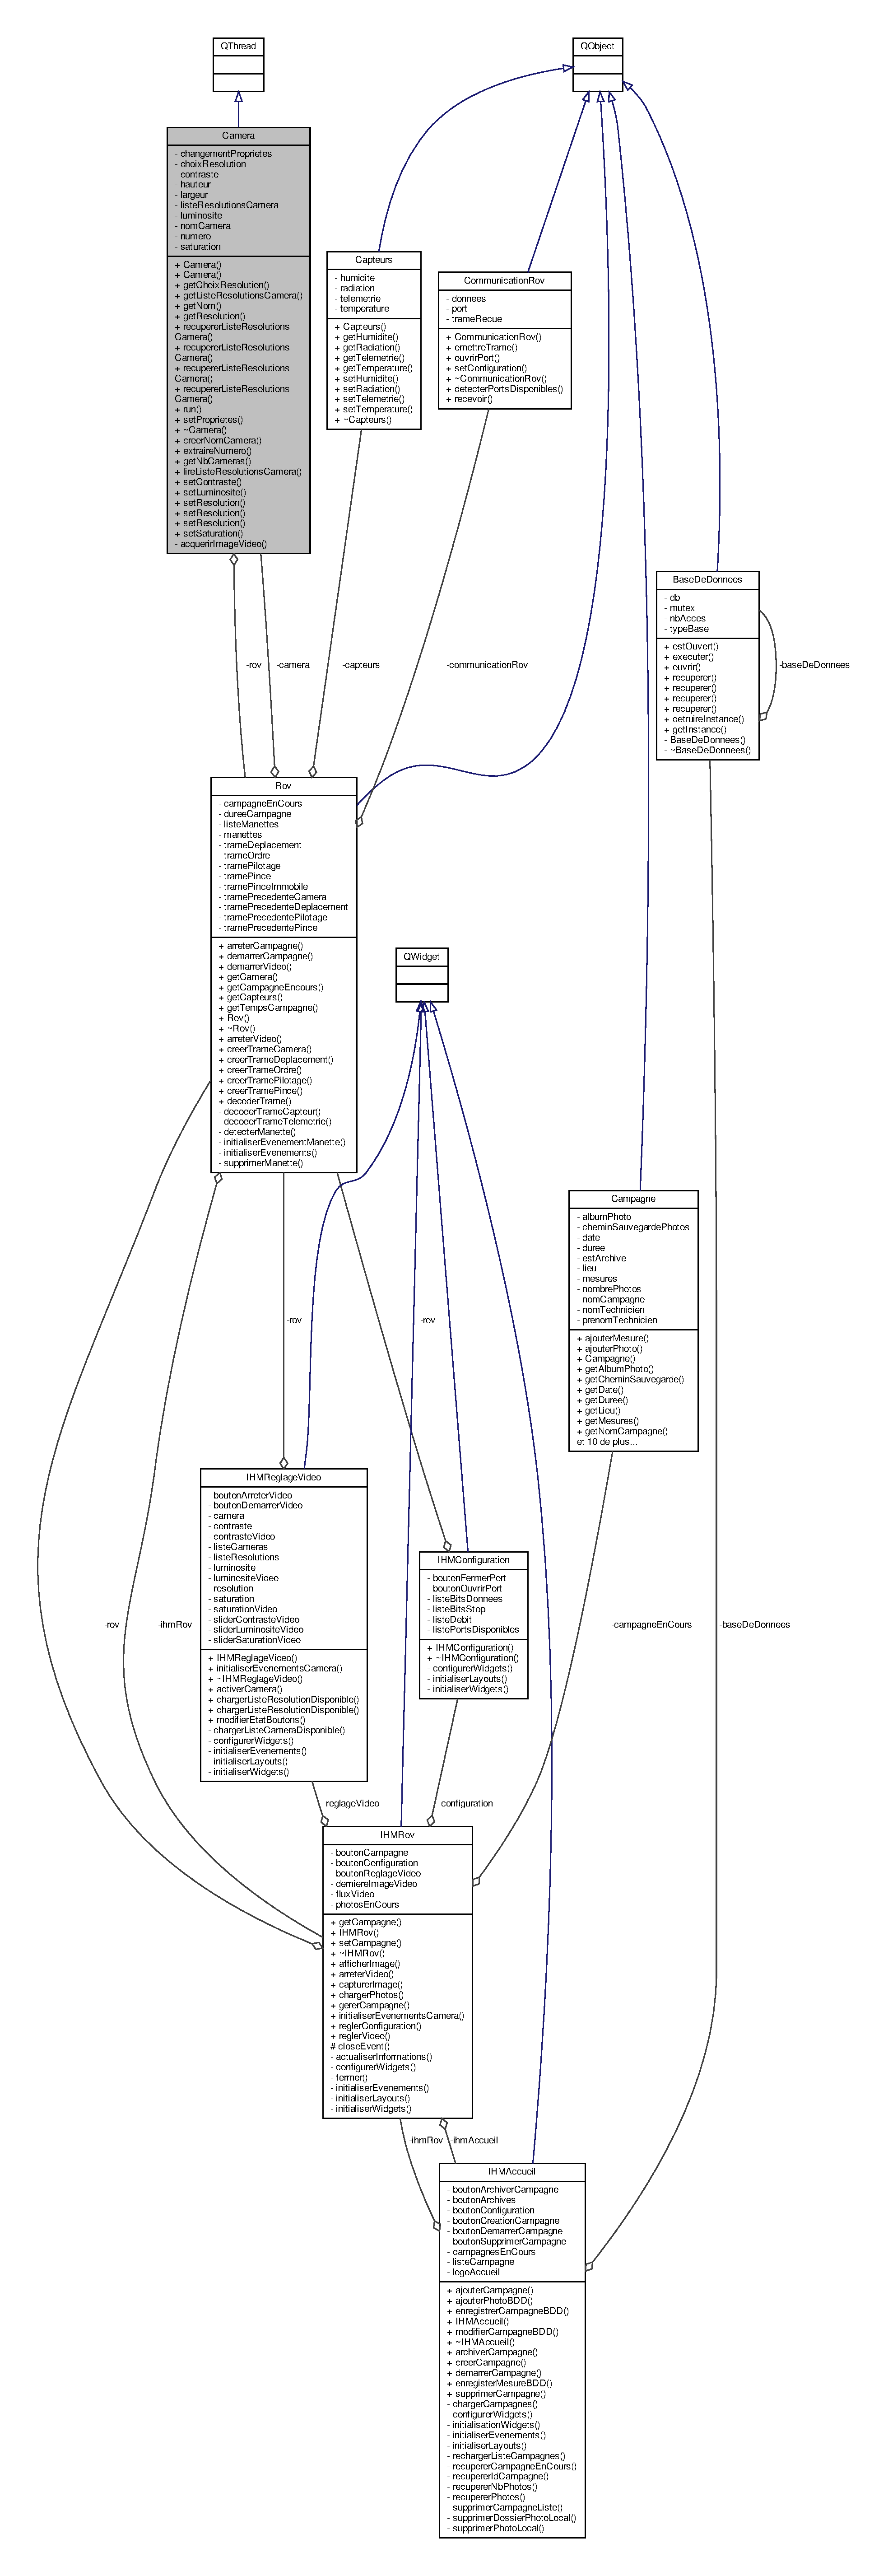
\includegraphics[height=550pt]{class_camera__coll__graph}
\end{center}
\end{figure}
\subsubsection*{Connecteurs publics}
\begin{DoxyCompactItemize}
\item 
void \hyperlink{class_camera_acc596f589be1e2e2d8e46e071ce38036}{set\+Contraste} (int \hyperlink{class_camera_ad3b300e52c91341d985d3b54f562a0f7}{contraste})
\begin{DoxyCompactList}\small\item\em Modifie le contraste de la caméra. \end{DoxyCompactList}\item 
void \hyperlink{class_camera_a25120dedc5f57638a866e1ff827fd641}{set\+Luminosite} (int \hyperlink{class_camera_aca5433bf19773161142d73009469b1ed}{luminosite})
\begin{DoxyCompactList}\small\item\em Modifie la luminosite de la caméra. \end{DoxyCompactList}\item 
void \hyperlink{class_camera_a966d13a5bf22c776f8d776d3da19182a}{set\+Resolution} (int \hyperlink{class_camera_ad64f26cdfc5aa561208b273d430938cf}{largeur}, int \hyperlink{class_camera_a5d89d7f9d1a5eab4175dd168c7fbf1c7}{hauteur})
\begin{DoxyCompactList}\small\item\em Modifie la résolution (largeur x hauteur) \end{DoxyCompactList}\item 
void \hyperlink{class_camera_a79630483bf9912a8fd1afe412ee8c848}{set\+Resolution} (Q\+Size resolution)
\begin{DoxyCompactList}\small\item\em Modifie la résolution (largeur x hauteur) \end{DoxyCompactList}\item 
void \hyperlink{class_camera_a7ff6343220c3ccd64ff513d2af37e1f3}{set\+Resolution} (int choix)
\begin{DoxyCompactList}\small\item\em Modifie la résolution (index dans la liste) \end{DoxyCompactList}\item 
void \hyperlink{class_camera_ace85018db120a6d61a5326172f97df93}{set\+Saturation} (int \hyperlink{class_camera_afd46d6d2451ee33b68dbc74713f2687c}{saturation})
\begin{DoxyCompactList}\small\item\em Modifie la saturation de la caméra. \end{DoxyCompactList}\end{DoxyCompactItemize}
\subsubsection*{Signaux}
\begin{DoxyCompactItemize}
\item 
void \hyperlink{class_camera_a4c560c4add60ebce65e2d9717e3d668c}{fin\+Video} ()
\begin{DoxyCompactList}\small\item\em Envoie un signal lorsque la vidéo est interrompu. \end{DoxyCompactList}\item 
void \hyperlink{class_camera_a38c810d466375e950401e483f885c52f}{nouvelle\+Image} (Q\+Pixmap image)
\begin{DoxyCompactList}\small\item\em Envoie un signal lorsque une nouvelle image du flux vidéo est disponible. \end{DoxyCompactList}\end{DoxyCompactItemize}
\subsubsection*{Fonctions membres publiques}
\begin{DoxyCompactItemize}
\item 
\hyperlink{class_camera_a26c49f76c98ece6ad6771351dd13583a}{Camera} (\hyperlink{class_rov}{Rov} $\ast$\hyperlink{class_camera_ad1dde4d981877001281af01c392307f1}{rov}, int \hyperlink{class_camera_ae5cda5df3c9c49b88fff15389a1bbc64}{numero}, int \hyperlink{class_camera_a3fdddf6f548f04d7bdc26f32602a03d4}{choix\+Resolution}=-\/1)
\begin{DoxyCompactList}\small\item\em Constructeur de la classe \hyperlink{class_camera}{Camera}. \end{DoxyCompactList}\item 
\hyperlink{class_camera_ae663da224161d1a78c8a7431ad1530d7}{Camera} (\hyperlink{class_rov}{Rov} $\ast$\hyperlink{class_camera_ad1dde4d981877001281af01c392307f1}{rov}, Q\+String \hyperlink{class_camera_ac1cdaf82921d2a2f3f941d867718eba2}{nom\+Camera}, int \hyperlink{class_camera_a3fdddf6f548f04d7bdc26f32602a03d4}{choix\+Resolution}=-\/1)
\begin{DoxyCompactList}\small\item\em Constructeur de la classe \hyperlink{class_camera}{Camera}. \end{DoxyCompactList}\item 
int \hyperlink{class_camera_ab9f05b05c29416dce6471b5a03db98ea}{get\+Choix\+Resolution} ()
\begin{DoxyCompactList}\small\item\em Récupère le choix de la resolution active. \end{DoxyCompactList}\item 
Q\+List$<$ Q\+Size $>$ \hyperlink{class_camera_a997441a0c1e33fe3eda800953548071d}{get\+Liste\+Resolutions\+Camera} ()
\begin{DoxyCompactList}\small\item\em Retourne la liste des résolutions supportées par la caméra. \end{DoxyCompactList}\item 
Q\+String \hyperlink{class_camera_a9b27a8a444006f40548a9a4ecf4d7256}{get\+Nom} () const
\begin{DoxyCompactList}\small\item\em Retourne le nom de la caméra. \end{DoxyCompactList}\item 
Q\+Size \hyperlink{class_camera_a9fae9d9b6fa352ff96c9874d9b085454}{get\+Resolution} ()
\begin{DoxyCompactList}\small\item\em Récupère la resolution active. \end{DoxyCompactList}\item 
void \hyperlink{class_camera_a97267488c5756b4217d4e1fbc68008fd}{recuperer\+Liste\+Resolutions\+Camera} ()
\begin{DoxyCompactList}\small\item\em Récupère la liste des résolutions supportées par la caméra sélectionnée. \end{DoxyCompactList}\item 
void \hyperlink{class_camera_acf7554fa133bab58c16192041254a1d6}{recuperer\+Liste\+Resolutions\+Camera} (int \hyperlink{class_camera_ae5cda5df3c9c49b88fff15389a1bbc64}{numero})
\begin{DoxyCompactList}\small\item\em Récupère la liste des résolutions supportées par la caméra à partir de son numéro. \end{DoxyCompactList}\item 
void \hyperlink{class_camera_ae3d1ccb26bcd49340bc392dc1e7bb550}{recuperer\+Liste\+Resolutions\+Camera} (Q\+String \hyperlink{class_camera_ac1cdaf82921d2a2f3f941d867718eba2}{nom\+Camera})
\begin{DoxyCompactList}\small\item\em Récupère la liste des résolutions supportées par la caméra à partir de son nom. \end{DoxyCompactList}\item 
void \hyperlink{class_camera_a4a9f1bcfa19bbd5add6c758c8ad85b5c}{recuperer\+Liste\+Resolutions\+Camera} (Q\+Camera\+Info \&camera\+Info)
\begin{DoxyCompactList}\small\item\em Récupère la liste des résolutions supporté par la caméra. \end{DoxyCompactList}\item 
void \hyperlink{class_camera_aaa3745c0cf0f286ef80b7eeebc248cc9}{run} ()
\begin{DoxyCompactList}\small\item\em Démarre une nouveau thread afin de capturer le flux video et l\textquotesingle{}envoyer à l\textquotesingle{}I\+HM. \end{DoxyCompactList}\item 
void \hyperlink{class_camera_a77397d68d606172ccfafed5624c31213}{set\+Proprietes} (cv\+::\+Video\+Capture \&camera)
\begin{DoxyCompactList}\small\item\em Après l\textquotesingle{}acquisition d\textquotesingle{}une nouvelle frame modifie les propriété de la caméra si ceux-\/ci ont été modifié par l\textquotesingle{}I\+HM. \end{DoxyCompactList}\item 
\hyperlink{class_camera_ad1897942d0ccf91052386388a497349f}{$\sim$\+Camera} ()
\begin{DoxyCompactList}\small\item\em Destructeur de la classe \hyperlink{class_camera}{Camera}. \end{DoxyCompactList}\end{DoxyCompactItemize}
\subsubsection*{Fonctions membres publiques statiques}
\begin{DoxyCompactItemize}
\item 
static Q\+String \hyperlink{class_camera_a506d459df95042a03894afd5b781c2aa}{creer\+Nom\+Camera} (int \hyperlink{class_camera_ae5cda5df3c9c49b88fff15389a1bbc64}{numero})
\begin{DoxyCompactList}\small\item\em Retourne le nom de caméra associé a son numéro. \end{DoxyCompactList}\item 
static int \hyperlink{class_camera_aa3fdc8b3feac7074911b472c4edb9dec}{extraire\+Numero} (Q\+String \hyperlink{class_camera_ac1cdaf82921d2a2f3f941d867718eba2}{nom\+Camera})
\begin{DoxyCompactList}\small\item\em Retourne le numéro de caméra associé a son nom. \end{DoxyCompactList}\item 
static int \hyperlink{class_camera_a116b3869ff0647c851715605a1938a3c}{get\+Nb\+Cameras} ()
\begin{DoxyCompactList}\small\item\em Retourne le nombre de caméras connectés. \end{DoxyCompactList}\item 
static Q\+List$<$ Q\+Size $>$ \hyperlink{class_camera_ac4756add4cb6bef60e38f3da79c2383f}{lire\+Liste\+Resolutions\+Camera} (Q\+Camera\+Info \&camera\+Info)
\begin{DoxyCompactList}\small\item\em Retourne la liste des résolutions supportés par la caméra passé en parametre. \end{DoxyCompactList}\end{DoxyCompactItemize}
\subsubsection*{Fonctions membres privées}
\begin{DoxyCompactItemize}
\item 
void \hyperlink{class_camera_afbddcda62053404cbf06a4ba48c62732}{acquerir\+Image\+Video} (cv\+::\+Video\+Capture \&camera, cv\+::\+Mat \&frame)
\begin{DoxyCompactList}\small\item\em Fait l\textquotesingle{}acquisition d\textquotesingle{}une nouvelle frame. \end{DoxyCompactList}\end{DoxyCompactItemize}
\subsubsection*{Attributs privés}
\begin{DoxyCompactItemize}
\item 
bool \hyperlink{class_camera_a50d2b3ef5c08f8b61bbe2115d71005bd}{changement\+Proprietes}
\begin{DoxyCompactList}\small\item\em Attribut désignant si une propriete de la caméra doit être modifiée. \end{DoxyCompactList}\item 
int \hyperlink{class_camera_a3fdddf6f548f04d7bdc26f32602a03d4}{choix\+Resolution}
\begin{DoxyCompactList}\small\item\em Choix dans la liste contenant les résolutions supportés par la caméra. \end{DoxyCompactList}\item 
double \hyperlink{class_camera_ad3b300e52c91341d985d3b54f562a0f7}{contraste}
\begin{DoxyCompactList}\small\item\em Attribut contenant le constraste de la vidéo. \end{DoxyCompactList}\item 
int \hyperlink{class_camera_a5d89d7f9d1a5eab4175dd168c7fbf1c7}{hauteur}
\begin{DoxyCompactList}\small\item\em Attribut contenant la hauteur (heigth) en pixels de la vidéo. \end{DoxyCompactList}\item 
int \hyperlink{class_camera_ad64f26cdfc5aa561208b273d430938cf}{largeur}
\begin{DoxyCompactList}\small\item\em Attribut contenant la largeur (width) en pixels de la vidéo. \end{DoxyCompactList}\item 
Q\+List$<$ Q\+Size $>$ \hyperlink{class_camera_a96af62eaf7828664865b56e7c69e771c}{liste\+Resolutions\+Camera}
\begin{DoxyCompactList}\small\item\em Liste contenant les résolutions supportés par la caméra. \end{DoxyCompactList}\item 
double \hyperlink{class_camera_aca5433bf19773161142d73009469b1ed}{luminosite}
\begin{DoxyCompactList}\small\item\em Attribut contenant la luminosite de la vidéo. \end{DoxyCompactList}\item 
Q\+String \hyperlink{class_camera_ac1cdaf82921d2a2f3f941d867718eba2}{nom\+Camera}
\begin{DoxyCompactList}\small\item\em Attribut contenant le nom de la caméra sélectionnée. \end{DoxyCompactList}\item 
int \hyperlink{class_camera_ae5cda5df3c9c49b88fff15389a1bbc64}{numero}
\begin{DoxyCompactList}\small\item\em Attribut contenant le numéro de la caméra sélectionnée. \end{DoxyCompactList}\item 
\hyperlink{class_rov}{Rov} $\ast$ \hyperlink{class_camera_ad1dde4d981877001281af01c392307f1}{rov}
\begin{DoxyCompactList}\small\item\em Objet rov permettant de récuperer les dernière mesures issues des capteurs. \end{DoxyCompactList}\item 
double \hyperlink{class_camera_afd46d6d2451ee33b68dbc74713f2687c}{saturation}
\begin{DoxyCompactList}\small\item\em Attribut contenant la saturation de la vidéo. \end{DoxyCompactList}\end{DoxyCompactItemize}


\subsubsection{Description détaillée}
Class permettant de mettre en place une communication avec la camera. 

Définition à la ligne \hyperlink{camera_8h_source_l00058}{58} du fichier \hyperlink{camera_8h_source}{camera.\+h}.



\subsubsection{Documentation des constructeurs et destructeur}
\mbox{\Hypertarget{class_camera_a26c49f76c98ece6ad6771351dd13583a}\label{class_camera_a26c49f76c98ece6ad6771351dd13583a}} 
\index{Camera@{Camera}!Camera@{Camera}}
\index{Camera@{Camera}!Camera@{Camera}}
\paragraph{\texorpdfstring{Camera()}{Camera()}\hspace{0.1cm}{\footnotesize\ttfamily [1/2]}}
{\footnotesize\ttfamily Camera\+::\+Camera (\begin{DoxyParamCaption}\item[{\hyperlink{class_rov}{Rov} $\ast$}]{rov,  }\item[{int}]{numero,  }\item[{int}]{choix\+Resolution = {\ttfamily -\/1} }\end{DoxyParamCaption})}



Constructeur de la classe \hyperlink{class_camera}{Camera}. 


\begin{DoxyParams}{Paramètres}
{\em rov} & \\
\hline
{\em numero} & \\
\hline
{\em choix\+Resolution} & \\
\hline
\end{DoxyParams}


Définition à la ligne \hyperlink{camera_8cpp_source_l00012}{12} du fichier \hyperlink{camera_8cpp_source}{camera.\+cpp}.



Références \hyperlink{camera_8h_source_l00068}{contraste}, \hyperlink{camera_8cpp_source_l00293}{creer\+Nom\+Camera()}, \hyperlink{camera_8cpp_source_l00270}{get\+Nb\+Cameras()}, \hyperlink{camera_8h_source_l00066}{hauteur}, \hyperlink{camera_8h_source_l00065}{largeur}, \hyperlink{camera_8h_source_l00067}{luminosite}, \hyperlink{camera_8h_source_l00063}{nom\+Camera}, \hyperlink{camera_8cpp_source_l00133}{recuperer\+Liste\+Resolutions\+Camera()}, \hyperlink{camera_8h_source_l00069}{saturation}, et \hyperlink{camera_8cpp_source_l00186}{set\+Resolution()}.


\begin{DoxyCode}
00012                                                        : \hyperlink{class_camera_ad1dde4d981877001281af01c392307f1}{rov}(rov), \hyperlink{class_camera_ae5cda5df3c9c49b88fff15389a1bbc64}{numero}(
      \hyperlink{class_camera_ae5cda5df3c9c49b88fff15389a1bbc64}{numero}), \hyperlink{class_camera_ad64f26cdfc5aa561208b273d430938cf}{largeur}(\hyperlink{camera_8h_afe66edd1ec0aa05058aaa2a069248f65}{LARGEUR\_DEFAUT}), \hyperlink{class_camera_a5d89d7f9d1a5eab4175dd168c7fbf1c7}{hauteur}(
      \hyperlink{camera_8h_a70cf269dc21e5a921c2927034d6cadd2}{HAUTEUR\_DEFAUT}), \hyperlink{class_camera_aca5433bf19773161142d73009469b1ed}{luminosite}(\hyperlink{camera_8h_ae340bfbdd3eec3bbbea7d39d91c8aa91}{SEUIL\_DEFAUT}), 
      \hyperlink{class_camera_ad3b300e52c91341d985d3b54f562a0f7}{contraste}(\hyperlink{camera_8h_ae340bfbdd3eec3bbbea7d39d91c8aa91}{SEUIL\_DEFAUT}), \hyperlink{class_camera_afd46d6d2451ee33b68dbc74713f2687c}{saturation}(\hyperlink{camera_8h_ae340bfbdd3eec3bbbea7d39d91c8aa91}{SEUIL\_DEFAUT}), 
      \hyperlink{class_camera_a50d2b3ef5c08f8b61bbe2115d71005bd}{changementProprietes}(\textcolor{keyword}{false}), \hyperlink{class_camera_a3fdddf6f548f04d7bdc26f32602a03d4}{choixResolution}(
      \hyperlink{class_camera_a3fdddf6f548f04d7bdc26f32602a03d4}{choixResolution})
00013 \{
00014 \textcolor{preprocessor}{    #if CV\_VERSION\_MAJOR == 3}
00015     qDebug() << Q\_FUNC\_INFO << \textcolor{stringliteral}{"OpenCV"} << CV\_VERSION\_MAJOR << CV\_VERSION\_MINOR;
00016 \textcolor{preprocessor}{    #else}
00017     qDebug() << Q\_FUNC\_INFO << \textcolor{stringliteral}{"OpenCV"} << CV\_MAJOR\_VERSION << CV\_MINOR\_VERSION;
00018 \textcolor{preprocessor}{    #endif}
00019 
00020     \hyperlink{class_camera_a116b3869ff0647c851715605a1938a3c}{Camera::getNbCameras}();
00021 
00022     \hyperlink{class_camera_ac1cdaf82921d2a2f3f941d867718eba2}{nomCamera} = \hyperlink{class_camera_a506d459df95042a03894afd5b781c2aa}{Camera::creerNomCamera}(\hyperlink{class_camera_ae5cda5df3c9c49b88fff15389a1bbc64}{numero});    
00023     \hyperlink{class_camera_a97267488c5756b4217d4e1fbc68008fd}{recupererListeResolutionsCamera}();
00024     \textcolor{keywordflow}{if}(\hyperlink{class_camera_a3fdddf6f548f04d7bdc26f32602a03d4}{choixResolution} == -1)
00025         \hyperlink{class_camera_a966d13a5bf22c776f8d776d3da19182a}{setResolution}(\hyperlink{class_camera_ad64f26cdfc5aa561208b273d430938cf}{largeur}, \hyperlink{class_camera_a5d89d7f9d1a5eab4175dd168c7fbf1c7}{hauteur});
00026     \textcolor{keywordflow}{else}
00027         \hyperlink{class_camera_a966d13a5bf22c776f8d776d3da19182a}{setResolution}(\hyperlink{class_camera_a3fdddf6f548f04d7bdc26f32602a03d4}{choixResolution});
00028     qDebug() << Q\_FUNC\_INFO << \textcolor{keyword}{this};
00029     qDebug() << Q\_FUNC\_INFO << \textcolor{stringliteral}{"numero"} << \hyperlink{class_camera_ae5cda5df3c9c49b88fff15389a1bbc64}{numero} << \textcolor{stringliteral}{"nomCamera"} << 
      \hyperlink{class_camera_ac1cdaf82921d2a2f3f941d867718eba2}{nomCamera};
00030     qDebug() << Q\_FUNC\_INFO << \textcolor{stringliteral}{"largeur"} << \hyperlink{class_camera_ad64f26cdfc5aa561208b273d430938cf}{largeur} << \textcolor{stringliteral}{"hauteur"} << 
      \hyperlink{class_camera_a5d89d7f9d1a5eab4175dd168c7fbf1c7}{hauteur};
00031     qDebug() << Q\_FUNC\_INFO << \textcolor{stringliteral}{"luminosite"} << \hyperlink{class_camera_aca5433bf19773161142d73009469b1ed}{luminosite} << \textcolor{stringliteral}{"contraste"} << 
      \hyperlink{class_camera_ad3b300e52c91341d985d3b54f562a0f7}{contraste} << \textcolor{stringliteral}{"saturation"} << \hyperlink{class_camera_afd46d6d2451ee33b68dbc74713f2687c}{saturation};
00032 \}
\end{DoxyCode}
\mbox{\Hypertarget{class_camera_ae663da224161d1a78c8a7431ad1530d7}\label{class_camera_ae663da224161d1a78c8a7431ad1530d7}} 
\index{Camera@{Camera}!Camera@{Camera}}
\index{Camera@{Camera}!Camera@{Camera}}
\paragraph{\texorpdfstring{Camera()}{Camera()}\hspace{0.1cm}{\footnotesize\ttfamily [2/2]}}
{\footnotesize\ttfamily Camera\+::\+Camera (\begin{DoxyParamCaption}\item[{\hyperlink{class_rov}{Rov} $\ast$}]{rov,  }\item[{Q\+String}]{nom\+Camera,  }\item[{int}]{choix\+Resolution = {\ttfamily -\/1} }\end{DoxyParamCaption})}



Constructeur de la classe \hyperlink{class_camera}{Camera}. 


\begin{DoxyParams}{Paramètres}
{\em rov} & \\
\hline
{\em nom\+Camera} & \\
\hline
{\em choix\+Resolution} & \\
\hline
\end{DoxyParams}


Définition à la ligne \hyperlink{camera_8cpp_source_l00034}{34} du fichier \hyperlink{camera_8cpp_source}{camera.\+cpp}.



Références \hyperlink{camera_8h_source_l00068}{contraste}, \hyperlink{camera_8cpp_source_l00276}{extraire\+Numero()}, \hyperlink{camera_8cpp_source_l00270}{get\+Nb\+Cameras()}, \hyperlink{camera_8h_source_l00066}{hauteur}, \hyperlink{camera_8h_source_l00065}{largeur}, \hyperlink{camera_8h_source_l00067}{luminosite}, \hyperlink{camera_8h_source_l00063}{nom\+Camera}, \hyperlink{camera_8h_source_l00064}{numero}, \hyperlink{camera_8cpp_source_l00133}{recuperer\+Liste\+Resolutions\+Camera()}, \hyperlink{camera_8h_source_l00069}{saturation}, et \hyperlink{camera_8cpp_source_l00186}{set\+Resolution()}.


\begin{DoxyCode}
00034                                                               : \hyperlink{class_camera_ad1dde4d981877001281af01c392307f1}{rov}(rov), 
      \hyperlink{class_camera_ac1cdaf82921d2a2f3f941d867718eba2}{nomCamera}(\hyperlink{class_camera_ac1cdaf82921d2a2f3f941d867718eba2}{nomCamera}), \hyperlink{class_camera_ad64f26cdfc5aa561208b273d430938cf}{largeur}(\hyperlink{camera_8h_afe66edd1ec0aa05058aaa2a069248f65}{LARGEUR\_DEFAUT}), 
      \hyperlink{class_camera_a5d89d7f9d1a5eab4175dd168c7fbf1c7}{hauteur}(\hyperlink{camera_8h_a70cf269dc21e5a921c2927034d6cadd2}{HAUTEUR\_DEFAUT}), \hyperlink{class_camera_aca5433bf19773161142d73009469b1ed}{luminosite}(\hyperlink{camera_8h_ae340bfbdd3eec3bbbea7d39d91c8aa91}{SEUIL\_DEFAUT}), 
      \hyperlink{class_camera_ad3b300e52c91341d985d3b54f562a0f7}{contraste}(\hyperlink{camera_8h_ae340bfbdd3eec3bbbea7d39d91c8aa91}{SEUIL\_DEFAUT}), \hyperlink{class_camera_afd46d6d2451ee33b68dbc74713f2687c}{saturation}(\hyperlink{camera_8h_ae340bfbdd3eec3bbbea7d39d91c8aa91}{SEUIL\_DEFAUT}), 
      \hyperlink{class_camera_a50d2b3ef5c08f8b61bbe2115d71005bd}{changementProprietes}(\textcolor{keyword}{false}), \hyperlink{class_camera_a3fdddf6f548f04d7bdc26f32602a03d4}{choixResolution}(
      \hyperlink{class_camera_a3fdddf6f548f04d7bdc26f32602a03d4}{choixResolution})
00035 \{
00036 \textcolor{preprocessor}{    #if CV\_VERSION\_MAJOR == 3}
00037     qDebug() << Q\_FUNC\_INFO << \textcolor{stringliteral}{"OpenCV"} << CV\_VERSION\_MAJOR << CV\_VERSION\_MINOR;
00038 \textcolor{preprocessor}{    #else}
00039     qDebug() << Q\_FUNC\_INFO << \textcolor{stringliteral}{"OpenCV"} << CV\_MAJOR\_VERSION << CV\_MINOR\_VERSION;
00040 \textcolor{preprocessor}{    #endif}
00041 
00042     \hyperlink{class_camera_a116b3869ff0647c851715605a1938a3c}{Camera::getNbCameras}();
00043 
00044     \hyperlink{class_camera_ae5cda5df3c9c49b88fff15389a1bbc64}{numero} = \hyperlink{class_camera_aa3fdc8b3feac7074911b472c4edb9dec}{Camera::extraireNumero}(\hyperlink{class_camera_ac1cdaf82921d2a2f3f941d867718eba2}{nomCamera});
00045 
00046     \hyperlink{class_camera_a97267488c5756b4217d4e1fbc68008fd}{recupererListeResolutionsCamera}();
00047     \textcolor{keywordflow}{if}(\hyperlink{class_camera_a3fdddf6f548f04d7bdc26f32602a03d4}{choixResolution} == -1)
00048         \hyperlink{class_camera_a966d13a5bf22c776f8d776d3da19182a}{setResolution}(\hyperlink{class_camera_ad64f26cdfc5aa561208b273d430938cf}{largeur}, \hyperlink{class_camera_a5d89d7f9d1a5eab4175dd168c7fbf1c7}{hauteur});
00049     \textcolor{keywordflow}{else}
00050         \hyperlink{class_camera_a966d13a5bf22c776f8d776d3da19182a}{setResolution}(\hyperlink{class_camera_a3fdddf6f548f04d7bdc26f32602a03d4}{choixResolution});
00051 
00052     qDebug() << Q\_FUNC\_INFO << \textcolor{keyword}{this};
00053     qDebug() << Q\_FUNC\_INFO << \textcolor{stringliteral}{"numero"} << \hyperlink{class_camera_ae5cda5df3c9c49b88fff15389a1bbc64}{numero} << \textcolor{stringliteral}{"nomCamera"} << 
      \hyperlink{class_camera_ac1cdaf82921d2a2f3f941d867718eba2}{nomCamera};
00054     qDebug() << Q\_FUNC\_INFO << \textcolor{stringliteral}{"largeur"} << \hyperlink{class_camera_ad64f26cdfc5aa561208b273d430938cf}{largeur} << \textcolor{stringliteral}{"hauteur"} << 
      \hyperlink{class_camera_a5d89d7f9d1a5eab4175dd168c7fbf1c7}{hauteur};
00055     qDebug() << Q\_FUNC\_INFO << \textcolor{stringliteral}{"luminosite"} << \hyperlink{class_camera_aca5433bf19773161142d73009469b1ed}{luminosite} << \textcolor{stringliteral}{"contraste"} << 
      \hyperlink{class_camera_ad3b300e52c91341d985d3b54f562a0f7}{contraste} << \textcolor{stringliteral}{"saturation"} << \hyperlink{class_camera_afd46d6d2451ee33b68dbc74713f2687c}{saturation};
00056 \}
\end{DoxyCode}
\mbox{\Hypertarget{class_camera_ad1897942d0ccf91052386388a497349f}\label{class_camera_ad1897942d0ccf91052386388a497349f}} 
\index{Camera@{Camera}!````~Camera@{$\sim$\+Camera}}
\index{````~Camera@{$\sim$\+Camera}!Camera@{Camera}}
\paragraph{\texorpdfstring{$\sim$\+Camera()}{~Camera()}}
{\footnotesize\ttfamily Camera\+::$\sim$\+Camera (\begin{DoxyParamCaption}{ }\end{DoxyParamCaption})}



Destructeur de la classe \hyperlink{class_camera}{Camera}. 



Définition à la ligne \hyperlink{camera_8cpp_source_l00058}{58} du fichier \hyperlink{camera_8cpp_source}{camera.\+cpp}.


\begin{DoxyCode}
00059 \{
00060     qDebug() << Q\_FUNC\_INFO << \textcolor{keyword}{this};
00061 \}
\end{DoxyCode}


\subsubsection{Documentation des fonctions membres}
\mbox{\Hypertarget{class_camera_afbddcda62053404cbf06a4ba48c62732}\label{class_camera_afbddcda62053404cbf06a4ba48c62732}} 
\index{Camera@{Camera}!acquerir\+Image\+Video@{acquerir\+Image\+Video}}
\index{acquerir\+Image\+Video@{acquerir\+Image\+Video}!Camera@{Camera}}
\paragraph{\texorpdfstring{acquerir\+Image\+Video()}{acquerirImageVideo()}}
{\footnotesize\ttfamily void Camera\+::acquerir\+Image\+Video (\begin{DoxyParamCaption}\item[{cv\+::\+Video\+Capture \&}]{camera,  }\item[{cv\+::\+Mat \&}]{frame }\end{DoxyParamCaption})\hspace{0.3cm}{\ttfamily [private]}}



Fait l\textquotesingle{}acquisition d\textquotesingle{}une nouvelle frame. 


\begin{DoxyParams}{Paramètres}
{\em camera} & \\
\hline
{\em frame} & \\
\hline
\end{DoxyParams}


Définition à la ligne \hyperlink{camera_8cpp_source_l00063}{63} du fichier \hyperlink{camera_8cpp_source}{camera.\+cpp}.



Référencé par \hyperlink{camera_8cpp_source_l00068}{run()}.


\begin{DoxyCode}
00064 \{
00065     camera >> frame;
00066 \}
\end{DoxyCode}
\mbox{\Hypertarget{class_camera_a506d459df95042a03894afd5b781c2aa}\label{class_camera_a506d459df95042a03894afd5b781c2aa}} 
\index{Camera@{Camera}!creer\+Nom\+Camera@{creer\+Nom\+Camera}}
\index{creer\+Nom\+Camera@{creer\+Nom\+Camera}!Camera@{Camera}}
\paragraph{\texorpdfstring{creer\+Nom\+Camera()}{creerNomCamera()}}
{\footnotesize\ttfamily Q\+String Camera\+::creer\+Nom\+Camera (\begin{DoxyParamCaption}\item[{int}]{numero }\end{DoxyParamCaption})\hspace{0.3cm}{\ttfamily [static]}}



Retourne le nom de caméra associé a son numéro. 

\begin{DoxyReturn}{Renvoie}
le nom de caméra associé a son numéro 
\end{DoxyReturn}

\begin{DoxyParams}{Paramètres}
{\em numero} & \\
\hline
\end{DoxyParams}


Définition à la ligne \hyperlink{camera_8cpp_source_l00293}{293} du fichier \hyperlink{camera_8cpp_source}{camera.\+cpp}.



Référencé par \hyperlink{camera_8cpp_source_l00012}{Camera()}, \hyperlink{rov_8cpp_source_l00123}{Rov\+::demarrer\+Campagne()}, et \hyperlink{camera_8cpp_source_l00139}{recuperer\+Liste\+Resolutions\+Camera()}.


\begin{DoxyCode}
00294 \{
00295     QString nom;
00296 
00297     \textcolor{keywordflow}{if}(\hyperlink{class_camera_ae5cda5df3c9c49b88fff15389a1bbc64}{numero} >= 0)
00298     \{
00299         nom = QString(\textcolor{stringliteral}{"/dev/video"}) + QString::number(\hyperlink{class_camera_ae5cda5df3c9c49b88fff15389a1bbc64}{numero});
00300     \}
00301     \textcolor{keywordflow}{return} nom;
00302 \}
\end{DoxyCode}
\mbox{\Hypertarget{class_camera_aa3fdc8b3feac7074911b472c4edb9dec}\label{class_camera_aa3fdc8b3feac7074911b472c4edb9dec}} 
\index{Camera@{Camera}!extraire\+Numero@{extraire\+Numero}}
\index{extraire\+Numero@{extraire\+Numero}!Camera@{Camera}}
\paragraph{\texorpdfstring{extraire\+Numero()}{extraireNumero()}}
{\footnotesize\ttfamily int Camera\+::extraire\+Numero (\begin{DoxyParamCaption}\item[{Q\+String}]{nom\+Camera }\end{DoxyParamCaption})\hspace{0.3cm}{\ttfamily [static]}}



Retourne le numéro de caméra associé a son nom. 

\begin{DoxyReturn}{Renvoie}
le numéro de caméra associé a son nom 
\end{DoxyReturn}

\begin{DoxyParams}{Paramètres}
{\em nom\+Camera} & \\
\hline
\end{DoxyParams}


Définition à la ligne \hyperlink{camera_8cpp_source_l00276}{276} du fichier \hyperlink{camera_8cpp_source}{camera.\+cpp}.



Références \hyperlink{camera_8h_source_l00064}{numero}.



Référencé par \hyperlink{camera_8cpp_source_l00034}{Camera()}.


\begin{DoxyCode}
00277 \{
00278     \textcolor{keywordtype}{int} \hyperlink{class_camera_ae5cda5df3c9c49b88fff15389a1bbc64}{numero} = -1;
00279     QString video = \textcolor{stringliteral}{"/dev/video"};
00280 
00281     \textcolor{keywordflow}{if}(\hyperlink{class_camera_ac1cdaf82921d2a2f3f941d867718eba2}{nomCamera}.contains(video))
00282     \{
00283         QString n = \hyperlink{class_camera_ac1cdaf82921d2a2f3f941d867718eba2}{nomCamera}.mid(video.length(), \hyperlink{class_camera_ac1cdaf82921d2a2f3f941d867718eba2}{nomCamera}.length());
00284         \textcolor{keywordtype}{bool} ok;
00285         qDebug() << Q\_FUNC\_INFO << \textcolor{stringliteral}{"nom"} << \hyperlink{class_camera_ac1cdaf82921d2a2f3f941d867718eba2}{nomCamera} << \textcolor{stringliteral}{"n"} << 
      \hyperlink{class_camera_ac1cdaf82921d2a2f3f941d867718eba2}{nomCamera}.right(\hyperlink{class_camera_ac1cdaf82921d2a2f3f941d867718eba2}{nomCamera}.indexOf(\textcolor{stringliteral}{"/dev/video"})) << \textcolor{stringliteral}{"index"} << 
      \hyperlink{class_camera_ac1cdaf82921d2a2f3f941d867718eba2}{nomCamera}.indexOf(\textcolor{stringliteral}{"/dev/video"});
00286         numero = n.toInt(&ok);
00287         \textcolor{keywordflow}{if}(ok)
00288             \textcolor{keywordflow}{return} \hyperlink{class_camera_ae5cda5df3c9c49b88fff15389a1bbc64}{numero};
00289     \}
00290     \textcolor{keywordflow}{return} \hyperlink{class_camera_ae5cda5df3c9c49b88fff15389a1bbc64}{numero};
00291 \}
\end{DoxyCode}
\mbox{\Hypertarget{class_camera_a4c560c4add60ebce65e2d9717e3d668c}\label{class_camera_a4c560c4add60ebce65e2d9717e3d668c}} 
\index{Camera@{Camera}!fin\+Video@{fin\+Video}}
\index{fin\+Video@{fin\+Video}!Camera@{Camera}}
\paragraph{\texorpdfstring{fin\+Video}{finVideo}}
{\footnotesize\ttfamily void Camera\+::fin\+Video (\begin{DoxyParamCaption}{ }\end{DoxyParamCaption})\hspace{0.3cm}{\ttfamily [signal]}}



Envoie un signal lorsque la vidéo est interrompu. 



Référencé par \hyperlink{camera_8cpp_source_l00068}{run()}.

\mbox{\Hypertarget{class_camera_ab9f05b05c29416dce6471b5a03db98ea}\label{class_camera_ab9f05b05c29416dce6471b5a03db98ea}} 
\index{Camera@{Camera}!get\+Choix\+Resolution@{get\+Choix\+Resolution}}
\index{get\+Choix\+Resolution@{get\+Choix\+Resolution}!Camera@{Camera}}
\paragraph{\texorpdfstring{get\+Choix\+Resolution()}{getChoixResolution()}}
{\footnotesize\ttfamily int Camera\+::get\+Choix\+Resolution (\begin{DoxyParamCaption}{ }\end{DoxyParamCaption})}



Récupère le choix de la resolution active. 

\begin{DoxyReturn}{Renvoie}
le choix de la resolution active 
\end{DoxyReturn}


Définition à la ligne \hyperlink{camera_8cpp_source_l00128}{128} du fichier \hyperlink{camera_8cpp_source}{camera.\+cpp}.



Références \hyperlink{camera_8h_source_l00072}{choix\+Resolution}.



Référencé par \hyperlink{ihmreglagevideo_8cpp_source_l00179}{I\+H\+M\+Reglage\+Video\+::charger\+Liste\+Resolution\+Disponible()}.


\begin{DoxyCode}
00129 \{
00130     \textcolor{keywordflow}{return} \hyperlink{class_camera_a3fdddf6f548f04d7bdc26f32602a03d4}{choixResolution};
00131 \}
\end{DoxyCode}
\mbox{\Hypertarget{class_camera_a997441a0c1e33fe3eda800953548071d}\label{class_camera_a997441a0c1e33fe3eda800953548071d}} 
\index{Camera@{Camera}!get\+Liste\+Resolutions\+Camera@{get\+Liste\+Resolutions\+Camera}}
\index{get\+Liste\+Resolutions\+Camera@{get\+Liste\+Resolutions\+Camera}!Camera@{Camera}}
\paragraph{\texorpdfstring{get\+Liste\+Resolutions\+Camera()}{getListeResolutionsCamera()}}
{\footnotesize\ttfamily Q\+List$<$ Q\+Size $>$ Camera\+::get\+Liste\+Resolutions\+Camera (\begin{DoxyParamCaption}{ }\end{DoxyParamCaption})}



Retourne la liste des résolutions supportées par la caméra. 

\begin{DoxyReturn}{Renvoie}
la liste des résolutions supportées par la caméra 
\end{DoxyReturn}


Définition à la ligne \hyperlink{camera_8cpp_source_l00181}{181} du fichier \hyperlink{camera_8cpp_source}{camera.\+cpp}.



Références \hyperlink{camera_8h_source_l00071}{liste\+Resolutions\+Camera}.


\begin{DoxyCode}
00182 \{
00183     \textcolor{keywordflow}{return} \hyperlink{class_camera_a96af62eaf7828664865b56e7c69e771c}{listeResolutionsCamera};
00184 \}
\end{DoxyCode}
\mbox{\Hypertarget{class_camera_a116b3869ff0647c851715605a1938a3c}\label{class_camera_a116b3869ff0647c851715605a1938a3c}} 
\index{Camera@{Camera}!get\+Nb\+Cameras@{get\+Nb\+Cameras}}
\index{get\+Nb\+Cameras@{get\+Nb\+Cameras}!Camera@{Camera}}
\paragraph{\texorpdfstring{get\+Nb\+Cameras()}{getNbCameras()}}
{\footnotesize\ttfamily int Camera\+::get\+Nb\+Cameras (\begin{DoxyParamCaption}{ }\end{DoxyParamCaption})\hspace{0.3cm}{\ttfamily [static]}}



Retourne le nombre de caméras connectés. 

\begin{DoxyReturn}{Renvoie}
le nombre de caméras connectés 
\end{DoxyReturn}


Définition à la ligne \hyperlink{camera_8cpp_source_l00270}{270} du fichier \hyperlink{camera_8cpp_source}{camera.\+cpp}.



Référencé par \hyperlink{camera_8cpp_source_l00012}{Camera()}, et \hyperlink{rov_8cpp_source_l00123}{Rov\+::demarrer\+Campagne()}.


\begin{DoxyCode}
00271 \{
00272     qDebug() << Q\_FUNC\_INFO  << \textcolor{stringliteral}{"Caméra(s) disponible(s)"} << QCameraInfo::availableCameras().count();
00273     \textcolor{keywordflow}{return} QCameraInfo::availableCameras().count();
00274 \}
\end{DoxyCode}
\mbox{\Hypertarget{class_camera_a9b27a8a444006f40548a9a4ecf4d7256}\label{class_camera_a9b27a8a444006f40548a9a4ecf4d7256}} 
\index{Camera@{Camera}!get\+Nom@{get\+Nom}}
\index{get\+Nom@{get\+Nom}!Camera@{Camera}}
\paragraph{\texorpdfstring{get\+Nom()}{getNom()}}
{\footnotesize\ttfamily Q\+String Camera\+::get\+Nom (\begin{DoxyParamCaption}{ }\end{DoxyParamCaption}) const}



Retourne le nom de la caméra. 

\begin{DoxyReturn}{Renvoie}
nom de la caméra 
\end{DoxyReturn}


Définition à la ligne \hyperlink{camera_8cpp_source_l00103}{103} du fichier \hyperlink{camera_8cpp_source}{camera.\+cpp}.



Références \hyperlink{camera_8h_source_l00063}{nom\+Camera}.



Référencé par \hyperlink{ihmreglagevideo_8cpp_source_l00132}{I\+H\+M\+Reglage\+Video\+::charger\+Liste\+Camera\+Disponible()}.


\begin{DoxyCode}
00104 \{
00105     \textcolor{keywordflow}{return} \hyperlink{class_camera_ac1cdaf82921d2a2f3f941d867718eba2}{nomCamera};
00106 \}
\end{DoxyCode}
\mbox{\Hypertarget{class_camera_a9fae9d9b6fa352ff96c9874d9b085454}\label{class_camera_a9fae9d9b6fa352ff96c9874d9b085454}} 
\index{Camera@{Camera}!get\+Resolution@{get\+Resolution}}
\index{get\+Resolution@{get\+Resolution}!Camera@{Camera}}
\paragraph{\texorpdfstring{get\+Resolution()}{getResolution()}}
{\footnotesize\ttfamily Q\+Size Camera\+::get\+Resolution (\begin{DoxyParamCaption}{ }\end{DoxyParamCaption})}



Récupère la resolution active. 

\begin{DoxyReturn}{Renvoie}
la resolution active 
\end{DoxyReturn}


Définition à la ligne \hyperlink{camera_8cpp_source_l00121}{121} du fichier \hyperlink{camera_8cpp_source}{camera.\+cpp}.



Références \hyperlink{camera_8h_source_l00072}{choix\+Resolution}, \hyperlink{camera_8h_source_l00041}{H\+A\+U\+T\+E\+U\+R\+\_\+\+D\+E\+F\+A\+UT}, \hyperlink{camera_8h_source_l00035}{L\+A\+R\+G\+E\+U\+R\+\_\+\+D\+E\+F\+A\+UT}, et \hyperlink{camera_8h_source_l00071}{liste\+Resolutions\+Camera}.



Référencé par \hyperlink{ihmreglagevideo_8cpp_source_l00179}{I\+H\+M\+Reglage\+Video\+::charger\+Liste\+Resolution\+Disponible()}.


\begin{DoxyCode}
00122 \{
00123     \textcolor{keywordflow}{if}(\hyperlink{class_camera_a3fdddf6f548f04d7bdc26f32602a03d4}{choixResolution} != -1)
00124         \textcolor{keywordflow}{return} \hyperlink{class_camera_a96af62eaf7828664865b56e7c69e771c}{listeResolutionsCamera}.at(\hyperlink{class_camera_a3fdddf6f548f04d7bdc26f32602a03d4}{choixResolution});
00125     \textcolor{keywordflow}{return} QSize(\hyperlink{camera_8h_afe66edd1ec0aa05058aaa2a069248f65}{LARGEUR\_DEFAUT},\hyperlink{camera_8h_a70cf269dc21e5a921c2927034d6cadd2}{HAUTEUR\_DEFAUT});
00126 \}
\end{DoxyCode}
\mbox{\Hypertarget{class_camera_ac4756add4cb6bef60e38f3da79c2383f}\label{class_camera_ac4756add4cb6bef60e38f3da79c2383f}} 
\index{Camera@{Camera}!lire\+Liste\+Resolutions\+Camera@{lire\+Liste\+Resolutions\+Camera}}
\index{lire\+Liste\+Resolutions\+Camera@{lire\+Liste\+Resolutions\+Camera}!Camera@{Camera}}
\paragraph{\texorpdfstring{lire\+Liste\+Resolutions\+Camera()}{lireListeResolutionsCamera()}}
{\footnotesize\ttfamily Q\+List$<$ Q\+Size $>$ Camera\+::lire\+Liste\+Resolutions\+Camera (\begin{DoxyParamCaption}\item[{Q\+Camera\+Info \&}]{camera\+Info }\end{DoxyParamCaption})\hspace{0.3cm}{\ttfamily [static]}}



Retourne la liste des résolutions supportés par la caméra passé en parametre. 

\begin{DoxyReturn}{Renvoie}
la liste des résolutions supportés par la caméra passé en parametre 
\end{DoxyReturn}

\begin{DoxyParams}{Paramètres}
{\em camera\+Info} & \\
\hline
\end{DoxyParams}


Définition à la ligne \hyperlink{camera_8cpp_source_l00304}{304} du fichier \hyperlink{camera_8cpp_source}{camera.\+cpp}.



Référencé par \hyperlink{ihmreglagevideo_8cpp_source_l00179}{I\+H\+M\+Reglage\+Video\+::charger\+Liste\+Resolution\+Disponible()}.


\begin{DoxyCode}
00305 \{
00306     QList<QSize> listeResolutions;
00307     listeResolutions.clear();
00308     \textcolor{keywordflow}{if}(QCameraInfo::availableCameras().count() > 0)
00309     \{
00310         QCamera *camera = \textcolor{keyword}{new} QCamera(cameraInfo);
00311         QMediaRecorder *mediaRecorder = \textcolor{keyword}{new} QMediaRecorder(camera);
00312         camera->load();
00313         qDebug() << Q\_FUNC\_INFO << mediaRecorder->supportedResolutions().size();
00314         \textcolor{keywordflow}{if}(mediaRecorder->supportedResolutions().size() > 0)
00315         \{
00316             \textcolor{keywordflow}{foreach} (\textcolor{keyword}{const} QSize &resolution, mediaRecorder->supportedResolutions())
00317             \{
00318                 qDebug() << Q\_FUNC\_INFO << resolution.width() << \textcolor{stringliteral}{"x"} << resolution.height();
00319                 listeResolutions.push\_back(resolution);
00320             \}
00321         \}
00322         \textcolor{keyword}{delete} mediaRecorder;
00323         \textcolor{keyword}{delete} camera;
00324     \}
00325     \textcolor{keywordflow}{return} listeResolutions;
00326 \}
\end{DoxyCode}
\mbox{\Hypertarget{class_camera_a38c810d466375e950401e483f885c52f}\label{class_camera_a38c810d466375e950401e483f885c52f}} 
\index{Camera@{Camera}!nouvelle\+Image@{nouvelle\+Image}}
\index{nouvelle\+Image@{nouvelle\+Image}!Camera@{Camera}}
\paragraph{\texorpdfstring{nouvelle\+Image}{nouvelleImage}}
{\footnotesize\ttfamily void Camera\+::nouvelle\+Image (\begin{DoxyParamCaption}\item[{Q\+Pixmap}]{image }\end{DoxyParamCaption})\hspace{0.3cm}{\ttfamily [signal]}}



Envoie un signal lorsque une nouvelle image du flux vidéo est disponible. 


\begin{DoxyParams}{Paramètres}
{\em image} & \\
\hline
\end{DoxyParams}


Référencé par \hyperlink{camera_8cpp_source_l00068}{run()}.

\mbox{\Hypertarget{class_camera_a97267488c5756b4217d4e1fbc68008fd}\label{class_camera_a97267488c5756b4217d4e1fbc68008fd}} 
\index{Camera@{Camera}!recuperer\+Liste\+Resolutions\+Camera@{recuperer\+Liste\+Resolutions\+Camera}}
\index{recuperer\+Liste\+Resolutions\+Camera@{recuperer\+Liste\+Resolutions\+Camera}!Camera@{Camera}}
\paragraph{\texorpdfstring{recuperer\+Liste\+Resolutions\+Camera()}{recupererListeResolutionsCamera()}\hspace{0.1cm}{\footnotesize\ttfamily [1/4]}}
{\footnotesize\ttfamily void Camera\+::recuperer\+Liste\+Resolutions\+Camera (\begin{DoxyParamCaption}{ }\end{DoxyParamCaption})}



Récupère la liste des résolutions supportées par la caméra sélectionnée. 



Définition à la ligne \hyperlink{camera_8cpp_source_l00133}{133} du fichier \hyperlink{camera_8cpp_source}{camera.\+cpp}.



Références \hyperlink{camera_8h_source_l00063}{nom\+Camera}.



Référencé par \hyperlink{camera_8cpp_source_l00012}{Camera()}, et \hyperlink{camera_8cpp_source_l00139}{recuperer\+Liste\+Resolutions\+Camera()}.


\begin{DoxyCode}
00134 \{
00135     QCameraInfo cameraInfo(\hyperlink{class_camera_ac1cdaf82921d2a2f3f941d867718eba2}{nomCamera}.toLatin1());
00136     \hyperlink{class_camera_a97267488c5756b4217d4e1fbc68008fd}{recupererListeResolutionsCamera}(cameraInfo);
00137 \}
\end{DoxyCode}
\mbox{\Hypertarget{class_camera_acf7554fa133bab58c16192041254a1d6}\label{class_camera_acf7554fa133bab58c16192041254a1d6}} 
\index{Camera@{Camera}!recuperer\+Liste\+Resolutions\+Camera@{recuperer\+Liste\+Resolutions\+Camera}}
\index{recuperer\+Liste\+Resolutions\+Camera@{recuperer\+Liste\+Resolutions\+Camera}!Camera@{Camera}}
\paragraph{\texorpdfstring{recuperer\+Liste\+Resolutions\+Camera()}{recupererListeResolutionsCamera()}\hspace{0.1cm}{\footnotesize\ttfamily [2/4]}}
{\footnotesize\ttfamily void Camera\+::recuperer\+Liste\+Resolutions\+Camera (\begin{DoxyParamCaption}\item[{int}]{numero }\end{DoxyParamCaption})}



Récupère la liste des résolutions supportées par la caméra à partir de son numéro. 


\begin{DoxyParams}{Paramètres}
{\em numero} & \\
\hline
\end{DoxyParams}


Définition à la ligne \hyperlink{camera_8cpp_source_l00139}{139} du fichier \hyperlink{camera_8cpp_source}{camera.\+cpp}.



Références \hyperlink{camera_8cpp_source_l00293}{creer\+Nom\+Camera()}, et \hyperlink{camera_8cpp_source_l00133}{recuperer\+Liste\+Resolutions\+Camera()}.


\begin{DoxyCode}
00140 \{
00141     QString nom = \hyperlink{class_camera_a506d459df95042a03894afd5b781c2aa}{Camera::creerNomCamera}(\hyperlink{class_camera_ae5cda5df3c9c49b88fff15389a1bbc64}{numero});
00142     QCameraInfo cameraInfo(nom.toLatin1());
00143     \hyperlink{class_camera_a97267488c5756b4217d4e1fbc68008fd}{recupererListeResolutionsCamera}(cameraInfo);
00144 \}
\end{DoxyCode}
\mbox{\Hypertarget{class_camera_ae3d1ccb26bcd49340bc392dc1e7bb550}\label{class_camera_ae3d1ccb26bcd49340bc392dc1e7bb550}} 
\index{Camera@{Camera}!recuperer\+Liste\+Resolutions\+Camera@{recuperer\+Liste\+Resolutions\+Camera}}
\index{recuperer\+Liste\+Resolutions\+Camera@{recuperer\+Liste\+Resolutions\+Camera}!Camera@{Camera}}
\paragraph{\texorpdfstring{recuperer\+Liste\+Resolutions\+Camera()}{recupererListeResolutionsCamera()}\hspace{0.1cm}{\footnotesize\ttfamily [3/4]}}
{\footnotesize\ttfamily void Camera\+::recuperer\+Liste\+Resolutions\+Camera (\begin{DoxyParamCaption}\item[{Q\+String}]{nom\+Camera }\end{DoxyParamCaption})}



Récupère la liste des résolutions supportées par la caméra à partir de son nom. 


\begin{DoxyParams}{Paramètres}
{\em nom\+Camera} & \\
\hline
\end{DoxyParams}


Définition à la ligne \hyperlink{camera_8cpp_source_l00146}{146} du fichier \hyperlink{camera_8cpp_source}{camera.\+cpp}.



Références \hyperlink{camera_8cpp_source_l00133}{recuperer\+Liste\+Resolutions\+Camera()}.


\begin{DoxyCode}
00147 \{
00148     QCameraInfo cameraInfo(\hyperlink{class_camera_ac1cdaf82921d2a2f3f941d867718eba2}{nomCamera}.toLatin1());
00149     \hyperlink{class_camera_a97267488c5756b4217d4e1fbc68008fd}{recupererListeResolutionsCamera}(cameraInfo);
00150 \}
\end{DoxyCode}
\mbox{\Hypertarget{class_camera_a4a9f1bcfa19bbd5add6c758c8ad85b5c}\label{class_camera_a4a9f1bcfa19bbd5add6c758c8ad85b5c}} 
\index{Camera@{Camera}!recuperer\+Liste\+Resolutions\+Camera@{recuperer\+Liste\+Resolutions\+Camera}}
\index{recuperer\+Liste\+Resolutions\+Camera@{recuperer\+Liste\+Resolutions\+Camera}!Camera@{Camera}}
\paragraph{\texorpdfstring{recuperer\+Liste\+Resolutions\+Camera()}{recupererListeResolutionsCamera()}\hspace{0.1cm}{\footnotesize\ttfamily [4/4]}}
{\footnotesize\ttfamily void Camera\+::recuperer\+Liste\+Resolutions\+Camera (\begin{DoxyParamCaption}\item[{Q\+Camera\+Info \&}]{camera\+Info }\end{DoxyParamCaption})}



Récupère la liste des résolutions supporté par la caméra. 


\begin{DoxyParams}{Paramètres}
{\em camera\+Info} & \\
\hline
\end{DoxyParams}


Définition à la ligne \hyperlink{camera_8cpp_source_l00152}{152} du fichier \hyperlink{camera_8cpp_source}{camera.\+cpp}.



Références \hyperlink{camera_8h_source_l00041}{H\+A\+U\+T\+E\+U\+R\+\_\+\+D\+E\+F\+A\+UT}, \hyperlink{camera_8h_source_l00035}{L\+A\+R\+G\+E\+U\+R\+\_\+\+D\+E\+F\+A\+UT}, et \hyperlink{camera_8h_source_l00071}{liste\+Resolutions\+Camera}.


\begin{DoxyCode}
00153 \{
00154 \textcolor{preprocessor}{    #ifndef SANS\_DETECTION}
00155     \hyperlink{class_camera_a96af62eaf7828664865b56e7c69e771c}{listeResolutionsCamera}.clear();
00156     \textcolor{keywordflow}{if}(QCameraInfo::availableCameras().count() > 0)
00157     \{
00158         QCamera *camera = \textcolor{keyword}{new} QCamera(cameraInfo, \textcolor{keyword}{this});
00159         QMediaRecorder *mediaRecorder = \textcolor{keyword}{new} QMediaRecorder(camera, \textcolor{keyword}{this});
00160         camera->load();
00161         qDebug() << Q\_FUNC\_INFO << \textcolor{keyword}{this} << mediaRecorder->supportedResolutions().size();
00162         \textcolor{keywordflow}{if}(mediaRecorder->supportedResolutions().size() > 0)
00163         \{
00164             \textcolor{keywordflow}{foreach} (\textcolor{keyword}{const} QSize &resolution, mediaRecorder->supportedResolutions())
00165             \{
00166                 qDebug() << Q\_FUNC\_INFO << resolution.width() << \textcolor{stringliteral}{"x"} << resolution.height();
00167                 \hyperlink{class_camera_a96af62eaf7828664865b56e7c69e771c}{listeResolutionsCamera}.push\_back(resolution);
00168             \}
00169         \}
00170         \textcolor{keyword}{delete} mediaRecorder;
00171         \textcolor{keyword}{delete} camera;
00172     \}
00173 \textcolor{preprocessor}{    #else}
00174     Q\_UNUSED(cameraInfo);
00175     \hyperlink{class_camera_a96af62eaf7828664865b56e7c69e771c}{listeResolutionsCamera}.clear();
00176     QSize resolutionDefaut(\hyperlink{camera_8h_afe66edd1ec0aa05058aaa2a069248f65}{LARGEUR\_DEFAUT}, \hyperlink{camera_8h_a70cf269dc21e5a921c2927034d6cadd2}{HAUTEUR\_DEFAUT});
00177     \hyperlink{class_camera_a96af62eaf7828664865b56e7c69e771c}{listeResolutionsCamera}.push\_back(resolutionDefaut);
00178 \textcolor{preprocessor}{    #endif}
00179 \}
\end{DoxyCode}
\mbox{\Hypertarget{class_camera_aaa3745c0cf0f286ef80b7eeebc248cc9}\label{class_camera_aaa3745c0cf0f286ef80b7eeebc248cc9}} 
\index{Camera@{Camera}!run@{run}}
\index{run@{run}!Camera@{Camera}}
\paragraph{\texorpdfstring{run()}{run()}}
{\footnotesize\ttfamily void Camera\+::run (\begin{DoxyParamCaption}{ }\end{DoxyParamCaption})}



Démarre une nouveau thread afin de capturer le flux video et l\textquotesingle{}envoyer à l\textquotesingle{}I\+HM. 



Définition à la ligne \hyperlink{camera_8cpp_source_l00068}{68} du fichier \hyperlink{camera_8cpp_source}{camera.\+cpp}.



Références \hyperlink{camera_8cpp_source_l00063}{acquerir\+Image\+Video()}, \hyperlink{camera_8h_source_l00070}{changement\+Proprietes}, \hyperlink{class_camera_a4c560c4add60ebce65e2d9717e3d668c}{fin\+Video()}, \hyperlink{camera_8h_source_l00063}{nom\+Camera}, \hyperlink{class_camera_a38c810d466375e950401e483f885c52f}{nouvelle\+Image()}, \hyperlink{camera_8h_source_l00064}{numero}, et \hyperlink{camera_8cpp_source_l00108}{set\+Proprietes()}.


\begin{DoxyCode}
00069 \{
00070     qDebug() << Q\_FUNC\_INFO << \textcolor{stringliteral}{"start"} << \textcolor{stringliteral}{"numero"} << \hyperlink{class_camera_ae5cda5df3c9c49b88fff15389a1bbc64}{numero} << \textcolor{stringliteral}{"nomCamera"} << 
      \hyperlink{class_camera_ac1cdaf82921d2a2f3f941d867718eba2}{nomCamera};
00071     this->setPriority(QThread::NormalPriority);
00072 
00073     \textcolor{keywordflow}{if}(\hyperlink{class_camera_ae5cda5df3c9c49b88fff15389a1bbc64}{numero} < 0)
00074     \{
00075         qDebug() << Q\_FUNC\_INFO  << \textcolor{stringliteral}{"Erreur numero"} << \hyperlink{class_camera_ae5cda5df3c9c49b88fff15389a1bbc64}{numero} << \textcolor{stringliteral}{"nomCamera"} << 
      \hyperlink{class_camera_ac1cdaf82921d2a2f3f941d867718eba2}{nomCamera};
00076         \textcolor{keywordflow}{return};
00077     \}
00078 
00079     cv::VideoCapture camera(\hyperlink{class_camera_ae5cda5df3c9c49b88fff15389a1bbc64}{numero});
00080     cv::Mat frame;
00081 
00082     \hyperlink{class_camera_a77397d68d606172ccfafed5624c31213}{setProprietes}(camera);
00083 
00084     \textcolor{keywordflow}{while}(camera.isOpened() && !isInterruptionRequested())
00085     \{
00086         \hyperlink{class_camera_afbddcda62053404cbf06a4ba48c62732}{acquerirImageVideo}(camera, frame);
00087         \textcolor{keywordflow}{if}(frame.empty())
00088             \textcolor{keywordflow}{continue};
00089 
00090         QPixmap pixmap = QPixmap::fromImage(QImage(frame.data, frame.cols, frame.rows, frame.step, 
      QImage::Format\_RGB888).rgbSwapped());
00091         emit \hyperlink{class_camera_a38c810d466375e950401e483f885c52f}{nouvelleImage}(pixmap);
00092 
00093         \textcolor{keywordflow}{if}(\hyperlink{class_camera_a50d2b3ef5c08f8b61bbe2115d71005bd}{changementProprietes})
00094             \hyperlink{class_camera_a77397d68d606172ccfafed5624c31213}{setProprietes}(camera);
00095     \}
00096 
00097     camera.release();
00098     qDebug() << Q\_FUNC\_INFO << \textcolor{stringliteral}{"stop"} << \textcolor{stringliteral}{"numero"} << \hyperlink{class_camera_ae5cda5df3c9c49b88fff15389a1bbc64}{numero} << \textcolor{stringliteral}{"nomCamera"} << 
      \hyperlink{class_camera_ac1cdaf82921d2a2f3f941d867718eba2}{nomCamera};
00099 
00100     emit \hyperlink{class_camera_a4c560c4add60ebce65e2d9717e3d668c}{finVideo}();
00101 \}
\end{DoxyCode}
\mbox{\Hypertarget{class_camera_acc596f589be1e2e2d8e46e071ce38036}\label{class_camera_acc596f589be1e2e2d8e46e071ce38036}} 
\index{Camera@{Camera}!set\+Contraste@{set\+Contraste}}
\index{set\+Contraste@{set\+Contraste}!Camera@{Camera}}
\paragraph{\texorpdfstring{set\+Contraste}{setContraste}}
{\footnotesize\ttfamily void Camera\+::set\+Contraste (\begin{DoxyParamCaption}\item[{int}]{contraste }\end{DoxyParamCaption})\hspace{0.3cm}{\ttfamily [slot]}}



Modifie le contraste de la caméra. 


\begin{DoxyParams}{Paramètres}
{\em contraste} & \\
\hline
\end{DoxyParams}


Définition à la ligne \hyperlink{camera_8cpp_source_l00258}{258} du fichier \hyperlink{camera_8cpp_source}{camera.\+cpp}.



Références \hyperlink{camera_8h_source_l00070}{changement\+Proprietes}.


\begin{DoxyCode}
00259 \{
00260     this->\hyperlink{class_camera_ad3b300e52c91341d985d3b54f562a0f7}{contraste} = double(\hyperlink{class_camera_ad3b300e52c91341d985d3b54f562a0f7}{contraste})/100;
00261     \hyperlink{class_camera_a50d2b3ef5c08f8b61bbe2115d71005bd}{changementProprietes} = \textcolor{keyword}{true};
00262 \}
\end{DoxyCode}
\mbox{\Hypertarget{class_camera_a25120dedc5f57638a866e1ff827fd641}\label{class_camera_a25120dedc5f57638a866e1ff827fd641}} 
\index{Camera@{Camera}!set\+Luminosite@{set\+Luminosite}}
\index{set\+Luminosite@{set\+Luminosite}!Camera@{Camera}}
\paragraph{\texorpdfstring{set\+Luminosite}{setLuminosite}}
{\footnotesize\ttfamily void Camera\+::set\+Luminosite (\begin{DoxyParamCaption}\item[{int}]{luminosite }\end{DoxyParamCaption})\hspace{0.3cm}{\ttfamily [slot]}}



Modifie la luminosite de la caméra. 


\begin{DoxyParams}{Paramètres}
{\em luminosite} & \\
\hline
\end{DoxyParams}


Définition à la ligne \hyperlink{camera_8cpp_source_l00252}{252} du fichier \hyperlink{camera_8cpp_source}{camera.\+cpp}.



Références \hyperlink{camera_8h_source_l00070}{changement\+Proprietes}.


\begin{DoxyCode}
00253 \{
00254     this->\hyperlink{class_camera_aca5433bf19773161142d73009469b1ed}{luminosite} = double(\hyperlink{class_camera_aca5433bf19773161142d73009469b1ed}{luminosite})/100;
00255     \hyperlink{class_camera_a50d2b3ef5c08f8b61bbe2115d71005bd}{changementProprietes} = \textcolor{keyword}{true};
00256 \}
\end{DoxyCode}
\mbox{\Hypertarget{class_camera_a77397d68d606172ccfafed5624c31213}\label{class_camera_a77397d68d606172ccfafed5624c31213}} 
\index{Camera@{Camera}!set\+Proprietes@{set\+Proprietes}}
\index{set\+Proprietes@{set\+Proprietes}!Camera@{Camera}}
\paragraph{\texorpdfstring{set\+Proprietes()}{setProprietes()}}
{\footnotesize\ttfamily void Camera\+::set\+Proprietes (\begin{DoxyParamCaption}\item[{cv\+::\+Video\+Capture \&}]{camera }\end{DoxyParamCaption})}



Après l\textquotesingle{}acquisition d\textquotesingle{}une nouvelle frame modifie les propriété de la caméra si ceux-\/ci ont été modifié par l\textquotesingle{}I\+HM. 


\begin{DoxyParams}{Paramètres}
{\em camera} & \\
\hline
\end{DoxyParams}


Définition à la ligne \hyperlink{camera_8cpp_source_l00108}{108} du fichier \hyperlink{camera_8cpp_source}{camera.\+cpp}.



Références \hyperlink{camera_8h_source_l00070}{changement\+Proprietes}, \hyperlink{camera_8h_source_l00068}{contraste}, \hyperlink{camera_8h_source_l00066}{hauteur}, \hyperlink{camera_8h_source_l00065}{largeur}, \hyperlink{camera_8h_source_l00067}{luminosite}, et \hyperlink{camera_8h_source_l00069}{saturation}.



Référencé par \hyperlink{camera_8cpp_source_l00068}{run()}.


\begin{DoxyCode}
00109 \{
00110     qDebug() << Q\_FUNC\_INFO << \textcolor{stringliteral}{"largeur"} << \hyperlink{class_camera_ad64f26cdfc5aa561208b273d430938cf}{largeur} << \textcolor{stringliteral}{"hauteur"} << 
      \hyperlink{class_camera_a5d89d7f9d1a5eab4175dd168c7fbf1c7}{hauteur};
00111     camera.set(CV\_CAP\_PROP\_FRAME\_WIDTH, \hyperlink{class_camera_ad64f26cdfc5aa561208b273d430938cf}{largeur});
00112     camera.set(CV\_CAP\_PROP\_FRAME\_HEIGHT, hauteur);
00113 
00114     qDebug() << Q\_FUNC\_INFO << \textcolor{stringliteral}{"luminosite"} << \hyperlink{class_camera_aca5433bf19773161142d73009469b1ed}{luminosite} << \textcolor{stringliteral}{"contraste"} << 
      \hyperlink{class_camera_ad3b300e52c91341d985d3b54f562a0f7}{contraste} << \textcolor{stringliteral}{"saturation"} << \hyperlink{class_camera_afd46d6d2451ee33b68dbc74713f2687c}{saturation};
00115     camera.set(CV\_CAP\_PROP\_BRIGHTNESS, \hyperlink{class_camera_aca5433bf19773161142d73009469b1ed}{luminosite});
00116     camera.set(CV\_CAP\_PROP\_CONTRAST, \hyperlink{class_camera_ad3b300e52c91341d985d3b54f562a0f7}{contraste});
00117     camera.set(CV\_CAP\_PROP\_SATURATION, saturation);
00118     \hyperlink{class_camera_a50d2b3ef5c08f8b61bbe2115d71005bd}{changementProprietes} = \textcolor{keyword}{false};
00119 \}
\end{DoxyCode}
\mbox{\Hypertarget{class_camera_a966d13a5bf22c776f8d776d3da19182a}\label{class_camera_a966d13a5bf22c776f8d776d3da19182a}} 
\index{Camera@{Camera}!set\+Resolution@{set\+Resolution}}
\index{set\+Resolution@{set\+Resolution}!Camera@{Camera}}
\paragraph{\texorpdfstring{set\+Resolution}{setResolution}\hspace{0.1cm}{\footnotesize\ttfamily [1/3]}}
{\footnotesize\ttfamily void Camera\+::set\+Resolution (\begin{DoxyParamCaption}\item[{int}]{largeur,  }\item[{int}]{hauteur }\end{DoxyParamCaption})\hspace{0.3cm}{\ttfamily [slot]}}



Modifie la résolution (largeur x hauteur) 


\begin{DoxyParams}{Paramètres}
{\em largeur} & \\
\hline
{\em hauteur} & \\
\hline
\end{DoxyParams}


Définition à la ligne \hyperlink{camera_8cpp_source_l00186}{186} du fichier \hyperlink{camera_8cpp_source}{camera.\+cpp}.



Références \hyperlink{camera_8h_source_l00070}{changement\+Proprietes}, \hyperlink{camera_8h_source_l00072}{choix\+Resolution}, \hyperlink{camera_8h_source_l00066}{hauteur}, \hyperlink{camera_8h_source_l00065}{largeur}, et \hyperlink{camera_8h_source_l00071}{liste\+Resolutions\+Camera}.



Référencé par \hyperlink{camera_8cpp_source_l00012}{Camera()}.


\begin{DoxyCode}
00187 \{    
00188     qDebug() << Q\_FUNC\_INFO << \textcolor{stringliteral}{"largeur"} << \hyperlink{class_camera_ad64f26cdfc5aa561208b273d430938cf}{largeur} << \textcolor{stringliteral}{"hauteur"} << 
      \hyperlink{class_camera_a5d89d7f9d1a5eab4175dd168c7fbf1c7}{hauteur};
00189     QSize size(\hyperlink{class_camera_ad64f26cdfc5aa561208b273d430938cf}{largeur}, hauteur);
00190     \textcolor{keywordtype}{int} i = \hyperlink{class_camera_a96af62eaf7828664865b56e7c69e771c}{listeResolutionsCamera}.indexOf(size);
00191     \textcolor{keywordflow}{if} (i != -1)
00192     \{
00193         \hyperlink{class_camera_a3fdddf6f548f04d7bdc26f32602a03d4}{choixResolution} = i;
00194         this->\hyperlink{class_camera_ad64f26cdfc5aa561208b273d430938cf}{largeur} = \hyperlink{class_camera_ad64f26cdfc5aa561208b273d430938cf}{largeur};
00195         this->hauteur = \hyperlink{class_camera_a5d89d7f9d1a5eab4175dd168c7fbf1c7}{hauteur};
00196         \hyperlink{class_camera_a50d2b3ef5c08f8b61bbe2115d71005bd}{changementProprietes} = \textcolor{keyword}{true};
00197     \}
00198     \textcolor{keywordflow}{else}
00199     \{
00200         size = \hyperlink{class_camera_a96af62eaf7828664865b56e7c69e771c}{listeResolutionsCamera}.last();
00201         \hyperlink{class_camera_a3fdddf6f548f04d7bdc26f32602a03d4}{choixResolution} = \hyperlink{class_camera_a96af62eaf7828664865b56e7c69e771c}{listeResolutionsCamera}.indexOf(size);;
00202         this->\hyperlink{class_camera_ad64f26cdfc5aa561208b273d430938cf}{largeur} = size.width();
00203         this->hauteur = size.height();
00204         \hyperlink{class_camera_a50d2b3ef5c08f8b61bbe2115d71005bd}{changementProprietes} = \textcolor{keyword}{true};
00205     \}
00206     qDebug() << Q\_FUNC\_INFO << \textcolor{stringliteral}{"largeur"} << this->\hyperlink{class_camera_ad64f26cdfc5aa561208b273d430938cf}{largeur} << \textcolor{stringliteral}{"hauteur"} << this->hauteur << \textcolor{stringliteral}{"
      choixResolution"} << \hyperlink{class_camera_a3fdddf6f548f04d7bdc26f32602a03d4}{choixResolution};
00207 \}
\end{DoxyCode}
\mbox{\Hypertarget{class_camera_a79630483bf9912a8fd1afe412ee8c848}\label{class_camera_a79630483bf9912a8fd1afe412ee8c848}} 
\index{Camera@{Camera}!set\+Resolution@{set\+Resolution}}
\index{set\+Resolution@{set\+Resolution}!Camera@{Camera}}
\paragraph{\texorpdfstring{set\+Resolution}{setResolution}\hspace{0.1cm}{\footnotesize\ttfamily [2/3]}}
{\footnotesize\ttfamily void Camera\+::set\+Resolution (\begin{DoxyParamCaption}\item[{Q\+Size}]{resolution }\end{DoxyParamCaption})\hspace{0.3cm}{\ttfamily [slot]}}



Modifie la résolution (largeur x hauteur) 


\begin{DoxyParams}{Paramètres}
{\em resolution} & (Q\+Size) \\
\hline
\end{DoxyParams}


Définition à la ligne \hyperlink{camera_8cpp_source_l00209}{209} du fichier \hyperlink{camera_8cpp_source}{camera.\+cpp}.



Références \hyperlink{camera_8h_source_l00070}{changement\+Proprietes}, \hyperlink{camera_8h_source_l00072}{choix\+Resolution}, \hyperlink{camera_8h_source_l00066}{hauteur}, \hyperlink{camera_8h_source_l00065}{largeur}, et \hyperlink{camera_8h_source_l00071}{liste\+Resolutions\+Camera}.


\begin{DoxyCode}
00210 \{
00211     qDebug() << Q\_FUNC\_INFO << \textcolor{stringliteral}{"largeur"} << resolution.width() << \textcolor{stringliteral}{"hauteur"} << resolution.height();
00212     \textcolor{keywordtype}{int} i = \hyperlink{class_camera_a96af62eaf7828664865b56e7c69e771c}{listeResolutionsCamera}.indexOf(resolution);
00213     \textcolor{keywordflow}{if} (i != -1)
00214     \{
00215         \hyperlink{class_camera_a3fdddf6f548f04d7bdc26f32602a03d4}{choixResolution} = i;
00216         this->\hyperlink{class_camera_ad64f26cdfc5aa561208b273d430938cf}{largeur} = resolution.width();
00217         this->\hyperlink{class_camera_a5d89d7f9d1a5eab4175dd168c7fbf1c7}{hauteur} = resolution.height();
00218         \hyperlink{class_camera_a50d2b3ef5c08f8b61bbe2115d71005bd}{changementProprietes} = \textcolor{keyword}{true};
00219     \}
00220     \textcolor{keywordflow}{else}
00221     \{
00222         QSize size = \hyperlink{class_camera_a96af62eaf7828664865b56e7c69e771c}{listeResolutionsCamera}.last();
00223         \hyperlink{class_camera_a3fdddf6f548f04d7bdc26f32602a03d4}{choixResolution} = \hyperlink{class_camera_a96af62eaf7828664865b56e7c69e771c}{listeResolutionsCamera}.indexOf(size);;
00224         this->\hyperlink{class_camera_ad64f26cdfc5aa561208b273d430938cf}{largeur} = size.width();
00225         this->\hyperlink{class_camera_a5d89d7f9d1a5eab4175dd168c7fbf1c7}{hauteur} = size.height();
00226         \hyperlink{class_camera_a50d2b3ef5c08f8b61bbe2115d71005bd}{changementProprietes} = \textcolor{keyword}{true};
00227     \}
00228     qDebug() << Q\_FUNC\_INFO << \textcolor{stringliteral}{"largeur"} << this->\hyperlink{class_camera_ad64f26cdfc5aa561208b273d430938cf}{largeur} << \textcolor{stringliteral}{"hauteur"} << this->
      \hyperlink{class_camera_a5d89d7f9d1a5eab4175dd168c7fbf1c7}{hauteur} << \textcolor{stringliteral}{"choixResolution"} << \hyperlink{class_camera_a3fdddf6f548f04d7bdc26f32602a03d4}{choixResolution};
00229 \}
\end{DoxyCode}
\mbox{\Hypertarget{class_camera_a7ff6343220c3ccd64ff513d2af37e1f3}\label{class_camera_a7ff6343220c3ccd64ff513d2af37e1f3}} 
\index{Camera@{Camera}!set\+Resolution@{set\+Resolution}}
\index{set\+Resolution@{set\+Resolution}!Camera@{Camera}}
\paragraph{\texorpdfstring{set\+Resolution}{setResolution}\hspace{0.1cm}{\footnotesize\ttfamily [3/3]}}
{\footnotesize\ttfamily void Camera\+::set\+Resolution (\begin{DoxyParamCaption}\item[{int}]{choix }\end{DoxyParamCaption})\hspace{0.3cm}{\ttfamily [slot]}}



Modifie la résolution (index dans la liste) 


\begin{DoxyParams}{Paramètres}
{\em choix} & \\
\hline
\end{DoxyParams}


Définition à la ligne \hyperlink{camera_8cpp_source_l00231}{231} du fichier \hyperlink{camera_8cpp_source}{camera.\+cpp}.



Références \hyperlink{camera_8h_source_l00070}{changement\+Proprietes}, \hyperlink{camera_8h_source_l00072}{choix\+Resolution}, \hyperlink{camera_8h_source_l00066}{hauteur}, \hyperlink{camera_8h_source_l00065}{largeur}, et \hyperlink{camera_8h_source_l00071}{liste\+Resolutions\+Camera}.


\begin{DoxyCode}
00232 \{
00233     qDebug() << Q\_FUNC\_INFO << \textcolor{stringliteral}{"choix"} << choix;
00234     \textcolor{keywordflow}{if}(choix < \hyperlink{class_camera_a96af62eaf7828664865b56e7c69e771c}{listeResolutionsCamera}.size())
00235     \{
00236         \hyperlink{class_camera_a3fdddf6f548f04d7bdc26f32602a03d4}{choixResolution} = choix;
00237         this->\hyperlink{class_camera_ad64f26cdfc5aa561208b273d430938cf}{largeur} = \hyperlink{class_camera_a96af62eaf7828664865b56e7c69e771c}{listeResolutionsCamera}.at(choix).width();
00238         this->\hyperlink{class_camera_a5d89d7f9d1a5eab4175dd168c7fbf1c7}{hauteur} = \hyperlink{class_camera_a96af62eaf7828664865b56e7c69e771c}{listeResolutionsCamera}.at(choix).height();
00239         \hyperlink{class_camera_a50d2b3ef5c08f8b61bbe2115d71005bd}{changementProprietes} = \textcolor{keyword}{true};
00240     \}
00241     \textcolor{keywordflow}{else}
00242     \{
00243         QSize size = \hyperlink{class_camera_a96af62eaf7828664865b56e7c69e771c}{listeResolutionsCamera}.last();
00244         \hyperlink{class_camera_a3fdddf6f548f04d7bdc26f32602a03d4}{choixResolution} = \hyperlink{class_camera_a96af62eaf7828664865b56e7c69e771c}{listeResolutionsCamera}.indexOf(size);;
00245         this->\hyperlink{class_camera_ad64f26cdfc5aa561208b273d430938cf}{largeur} = size.width();
00246         this->\hyperlink{class_camera_a5d89d7f9d1a5eab4175dd168c7fbf1c7}{hauteur} = size.height();
00247         \hyperlink{class_camera_a50d2b3ef5c08f8b61bbe2115d71005bd}{changementProprietes} = \textcolor{keyword}{true};
00248     \}
00249     qDebug() << Q\_FUNC\_INFO << \textcolor{stringliteral}{"largeur"} << this->\hyperlink{class_camera_ad64f26cdfc5aa561208b273d430938cf}{largeur} << \textcolor{stringliteral}{"hauteur"} << this->
      \hyperlink{class_camera_a5d89d7f9d1a5eab4175dd168c7fbf1c7}{hauteur} << \textcolor{stringliteral}{"choixResolution"} << \hyperlink{class_camera_a3fdddf6f548f04d7bdc26f32602a03d4}{choixResolution};
00250 \}
\end{DoxyCode}
\mbox{\Hypertarget{class_camera_ace85018db120a6d61a5326172f97df93}\label{class_camera_ace85018db120a6d61a5326172f97df93}} 
\index{Camera@{Camera}!set\+Saturation@{set\+Saturation}}
\index{set\+Saturation@{set\+Saturation}!Camera@{Camera}}
\paragraph{\texorpdfstring{set\+Saturation}{setSaturation}}
{\footnotesize\ttfamily void Camera\+::set\+Saturation (\begin{DoxyParamCaption}\item[{int}]{saturation }\end{DoxyParamCaption})\hspace{0.3cm}{\ttfamily [slot]}}



Modifie la saturation de la caméra. 


\begin{DoxyParams}{Paramètres}
{\em saturation} & \\
\hline
\end{DoxyParams}


Définition à la ligne \hyperlink{camera_8cpp_source_l00264}{264} du fichier \hyperlink{camera_8cpp_source}{camera.\+cpp}.



Références \hyperlink{camera_8h_source_l00070}{changement\+Proprietes}.


\begin{DoxyCode}
00265 \{
00266     this->\hyperlink{class_camera_afd46d6d2451ee33b68dbc74713f2687c}{saturation} = double(\hyperlink{class_camera_afd46d6d2451ee33b68dbc74713f2687c}{saturation})/100;
00267     \hyperlink{class_camera_a50d2b3ef5c08f8b61bbe2115d71005bd}{changementProprietes} = \textcolor{keyword}{true};
00268 \}
\end{DoxyCode}


\subsubsection{Documentation des données membres}
\mbox{\Hypertarget{class_camera_a50d2b3ef5c08f8b61bbe2115d71005bd}\label{class_camera_a50d2b3ef5c08f8b61bbe2115d71005bd}} 
\index{Camera@{Camera}!changement\+Proprietes@{changement\+Proprietes}}
\index{changement\+Proprietes@{changement\+Proprietes}!Camera@{Camera}}
\paragraph{\texorpdfstring{changement\+Proprietes}{changementProprietes}}
{\footnotesize\ttfamily bool Camera\+::changement\+Proprietes\hspace{0.3cm}{\ttfamily [private]}}



Attribut désignant si une propriete de la caméra doit être modifiée. 



Définition à la ligne \hyperlink{camera_8h_source_l00070}{70} du fichier \hyperlink{camera_8h_source}{camera.\+h}.



Référencé par \hyperlink{camera_8cpp_source_l00068}{run()}, \hyperlink{camera_8cpp_source_l00258}{set\+Contraste()}, \hyperlink{camera_8cpp_source_l00252}{set\+Luminosite()}, \hyperlink{camera_8cpp_source_l00108}{set\+Proprietes()}, \hyperlink{camera_8cpp_source_l00186}{set\+Resolution()}, et \hyperlink{camera_8cpp_source_l00264}{set\+Saturation()}.

\mbox{\Hypertarget{class_camera_a3fdddf6f548f04d7bdc26f32602a03d4}\label{class_camera_a3fdddf6f548f04d7bdc26f32602a03d4}} 
\index{Camera@{Camera}!choix\+Resolution@{choix\+Resolution}}
\index{choix\+Resolution@{choix\+Resolution}!Camera@{Camera}}
\paragraph{\texorpdfstring{choix\+Resolution}{choixResolution}}
{\footnotesize\ttfamily int Camera\+::choix\+Resolution\hspace{0.3cm}{\ttfamily [private]}}



Choix dans la liste contenant les résolutions supportés par la caméra. 



Définition à la ligne \hyperlink{camera_8h_source_l00072}{72} du fichier \hyperlink{camera_8h_source}{camera.\+h}.



Référencé par \hyperlink{camera_8cpp_source_l00128}{get\+Choix\+Resolution()}, \hyperlink{camera_8cpp_source_l00121}{get\+Resolution()}, et \hyperlink{camera_8cpp_source_l00186}{set\+Resolution()}.

\mbox{\Hypertarget{class_camera_ad3b300e52c91341d985d3b54f562a0f7}\label{class_camera_ad3b300e52c91341d985d3b54f562a0f7}} 
\index{Camera@{Camera}!contraste@{contraste}}
\index{contraste@{contraste}!Camera@{Camera}}
\paragraph{\texorpdfstring{contraste}{contraste}}
{\footnotesize\ttfamily double Camera\+::contraste\hspace{0.3cm}{\ttfamily [private]}}



Attribut contenant le constraste de la vidéo. 



Définition à la ligne \hyperlink{camera_8h_source_l00068}{68} du fichier \hyperlink{camera_8h_source}{camera.\+h}.



Référencé par \hyperlink{camera_8cpp_source_l00012}{Camera()}, et \hyperlink{camera_8cpp_source_l00108}{set\+Proprietes()}.

\mbox{\Hypertarget{class_camera_a5d89d7f9d1a5eab4175dd168c7fbf1c7}\label{class_camera_a5d89d7f9d1a5eab4175dd168c7fbf1c7}} 
\index{Camera@{Camera}!hauteur@{hauteur}}
\index{hauteur@{hauteur}!Camera@{Camera}}
\paragraph{\texorpdfstring{hauteur}{hauteur}}
{\footnotesize\ttfamily int Camera\+::hauteur\hspace{0.3cm}{\ttfamily [private]}}



Attribut contenant la hauteur (heigth) en pixels de la vidéo. 



Définition à la ligne \hyperlink{camera_8h_source_l00066}{66} du fichier \hyperlink{camera_8h_source}{camera.\+h}.



Référencé par \hyperlink{camera_8cpp_source_l00012}{Camera()}, \hyperlink{camera_8cpp_source_l00108}{set\+Proprietes()}, et \hyperlink{camera_8cpp_source_l00186}{set\+Resolution()}.

\mbox{\Hypertarget{class_camera_ad64f26cdfc5aa561208b273d430938cf}\label{class_camera_ad64f26cdfc5aa561208b273d430938cf}} 
\index{Camera@{Camera}!largeur@{largeur}}
\index{largeur@{largeur}!Camera@{Camera}}
\paragraph{\texorpdfstring{largeur}{largeur}}
{\footnotesize\ttfamily int Camera\+::largeur\hspace{0.3cm}{\ttfamily [private]}}



Attribut contenant la largeur (width) en pixels de la vidéo. 



Définition à la ligne \hyperlink{camera_8h_source_l00065}{65} du fichier \hyperlink{camera_8h_source}{camera.\+h}.



Référencé par \hyperlink{camera_8cpp_source_l00012}{Camera()}, \hyperlink{camera_8cpp_source_l00108}{set\+Proprietes()}, et \hyperlink{camera_8cpp_source_l00186}{set\+Resolution()}.

\mbox{\Hypertarget{class_camera_a96af62eaf7828664865b56e7c69e771c}\label{class_camera_a96af62eaf7828664865b56e7c69e771c}} 
\index{Camera@{Camera}!liste\+Resolutions\+Camera@{liste\+Resolutions\+Camera}}
\index{liste\+Resolutions\+Camera@{liste\+Resolutions\+Camera}!Camera@{Camera}}
\paragraph{\texorpdfstring{liste\+Resolutions\+Camera}{listeResolutionsCamera}}
{\footnotesize\ttfamily Q\+List$<$Q\+Size$>$ Camera\+::liste\+Resolutions\+Camera\hspace{0.3cm}{\ttfamily [private]}}



Liste contenant les résolutions supportés par la caméra. 



Définition à la ligne \hyperlink{camera_8h_source_l00071}{71} du fichier \hyperlink{camera_8h_source}{camera.\+h}.



Référencé par \hyperlink{camera_8cpp_source_l00181}{get\+Liste\+Resolutions\+Camera()}, \hyperlink{camera_8cpp_source_l00121}{get\+Resolution()}, \hyperlink{camera_8cpp_source_l00152}{recuperer\+Liste\+Resolutions\+Camera()}, et \hyperlink{camera_8cpp_source_l00186}{set\+Resolution()}.

\mbox{\Hypertarget{class_camera_aca5433bf19773161142d73009469b1ed}\label{class_camera_aca5433bf19773161142d73009469b1ed}} 
\index{Camera@{Camera}!luminosite@{luminosite}}
\index{luminosite@{luminosite}!Camera@{Camera}}
\paragraph{\texorpdfstring{luminosite}{luminosite}}
{\footnotesize\ttfamily double Camera\+::luminosite\hspace{0.3cm}{\ttfamily [private]}}



Attribut contenant la luminosite de la vidéo. 



Définition à la ligne \hyperlink{camera_8h_source_l00067}{67} du fichier \hyperlink{camera_8h_source}{camera.\+h}.



Référencé par \hyperlink{camera_8cpp_source_l00012}{Camera()}, et \hyperlink{camera_8cpp_source_l00108}{set\+Proprietes()}.

\mbox{\Hypertarget{class_camera_ac1cdaf82921d2a2f3f941d867718eba2}\label{class_camera_ac1cdaf82921d2a2f3f941d867718eba2}} 
\index{Camera@{Camera}!nom\+Camera@{nom\+Camera}}
\index{nom\+Camera@{nom\+Camera}!Camera@{Camera}}
\paragraph{\texorpdfstring{nom\+Camera}{nomCamera}}
{\footnotesize\ttfamily Q\+String Camera\+::nom\+Camera\hspace{0.3cm}{\ttfamily [private]}}



Attribut contenant le nom de la caméra sélectionnée. 



Définition à la ligne \hyperlink{camera_8h_source_l00063}{63} du fichier \hyperlink{camera_8h_source}{camera.\+h}.



Référencé par \hyperlink{camera_8cpp_source_l00012}{Camera()}, \hyperlink{camera_8cpp_source_l00103}{get\+Nom()}, \hyperlink{camera_8cpp_source_l00133}{recuperer\+Liste\+Resolutions\+Camera()}, et \hyperlink{camera_8cpp_source_l00068}{run()}.

\mbox{\Hypertarget{class_camera_ae5cda5df3c9c49b88fff15389a1bbc64}\label{class_camera_ae5cda5df3c9c49b88fff15389a1bbc64}} 
\index{Camera@{Camera}!numero@{numero}}
\index{numero@{numero}!Camera@{Camera}}
\paragraph{\texorpdfstring{numero}{numero}}
{\footnotesize\ttfamily int Camera\+::numero\hspace{0.3cm}{\ttfamily [private]}}



Attribut contenant le numéro de la caméra sélectionnée. 



Définition à la ligne \hyperlink{camera_8h_source_l00064}{64} du fichier \hyperlink{camera_8h_source}{camera.\+h}.



Référencé par \hyperlink{camera_8cpp_source_l00034}{Camera()}, \hyperlink{camera_8cpp_source_l00276}{extraire\+Numero()}, et \hyperlink{camera_8cpp_source_l00068}{run()}.

\mbox{\Hypertarget{class_camera_ad1dde4d981877001281af01c392307f1}\label{class_camera_ad1dde4d981877001281af01c392307f1}} 
\index{Camera@{Camera}!rov@{rov}}
\index{rov@{rov}!Camera@{Camera}}
\paragraph{\texorpdfstring{rov}{rov}}
{\footnotesize\ttfamily \hyperlink{class_rov}{Rov}$\ast$ Camera\+::rov\hspace{0.3cm}{\ttfamily [private]}}



Objet rov permettant de récuperer les dernière mesures issues des capteurs. 



Définition à la ligne \hyperlink{camera_8h_source_l00062}{62} du fichier \hyperlink{camera_8h_source}{camera.\+h}.

\mbox{\Hypertarget{class_camera_afd46d6d2451ee33b68dbc74713f2687c}\label{class_camera_afd46d6d2451ee33b68dbc74713f2687c}} 
\index{Camera@{Camera}!saturation@{saturation}}
\index{saturation@{saturation}!Camera@{Camera}}
\paragraph{\texorpdfstring{saturation}{saturation}}
{\footnotesize\ttfamily double Camera\+::saturation\hspace{0.3cm}{\ttfamily [private]}}



Attribut contenant la saturation de la vidéo. 



Définition à la ligne \hyperlink{camera_8h_source_l00069}{69} du fichier \hyperlink{camera_8h_source}{camera.\+h}.



Référencé par \hyperlink{camera_8cpp_source_l00012}{Camera()}, et \hyperlink{camera_8cpp_source_l00108}{set\+Proprietes()}.



La documentation de cette classe a été générée à partir des fichiers suivants \+:\begin{DoxyCompactItemize}
\item 
\hyperlink{camera_8h}{camera.\+h}\item 
\hyperlink{camera_8cpp}{camera.\+cpp}\end{DoxyCompactItemize}

\hypertarget{class_campagne}{}\subsection{Référence de la classe Campagne}
\label{class_campagne}\index{Campagne@{Campagne}}


Class contenant les informations de la campagne en cours.  




{\ttfamily \#include \char`\"{}campagne.\+h\char`\"{}}



Graphe de collaboration de Campagne\+:
\nopagebreak
\begin{figure}[H]
\begin{center}
\leavevmode
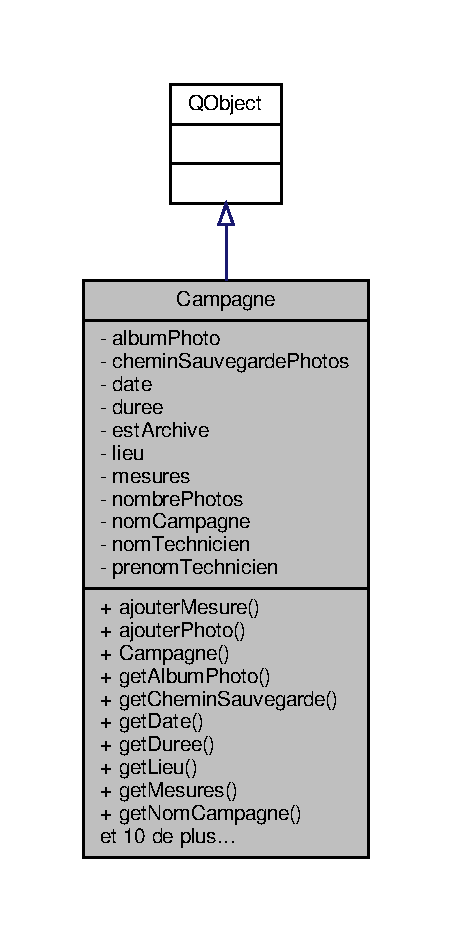
\includegraphics[width=217pt]{class_campagne__coll__graph}
\end{center}
\end{figure}
\subsubsection*{Fonctions membres publiques}
\begin{DoxyCompactItemize}
\item 
void \hyperlink{class_campagne_ab301ceaacbe1186682c2b6f3282619d0}{ajouter\+Mesure} (\hyperlink{struct_mesure}{Mesure} \&mesure)
\begin{DoxyCompactList}\small\item\em Ajoute une mesure dans le conteneur de mesure. \end{DoxyCompactList}\item 
void \hyperlink{class_campagne_a472029bf46646d136a750dbaa7a3155f}{ajouter\+Photo} (\hyperlink{struct_photo}{Photo} \&photo)
\begin{DoxyCompactList}\small\item\em Ajoute une photo dans l\textquotesingle{}album photo. \end{DoxyCompactList}\item 
\hyperlink{class_campagne_aba78ce7d7b921053abc69e22789ec6da}{Campagne} (Q\+String \hyperlink{class_campagne_a4455078418041442fa3998b9b6cb6230}{nom\+Campagne}, Q\+String \hyperlink{class_campagne_a1df66832d5d700bfd2bd36fe548f7cba}{lieu}, Q\+String \hyperlink{class_campagne_a6d3e88fb93b38cbcf1bc53cc9fc30f2f}{nom\+Technicien}, Q\+String \hyperlink{class_campagne_a9cc37c9671136683b5dac87ff34017bc}{prenom\+Technicien}, Q\+Date\+Time \hyperlink{class_campagne_ac8180e3e533648770c4e6d9a182fe3ed}{date}, \hyperlink{class_q_object}{Q\+Object} $\ast$parent=nullptr, int \hyperlink{class_campagne_a4fb4cb286275103c9b6946e25e301fbf}{duree}=0)
\begin{DoxyCompactList}\small\item\em Constructeur de la classe \hyperlink{class_campagne}{Campagne}. \end{DoxyCompactList}\item 
Q\+Vector$<$ \hyperlink{struct_photo}{Photo} $>$ \hyperlink{class_campagne_abec90fcbc0c4ded45caaac9adb454add}{get\+Album\+Photo} () const
\begin{DoxyCompactList}\small\item\em Retourne l\textquotesingle{}album photo de la campagne. \end{DoxyCompactList}\item 
Q\+String \hyperlink{class_campagne_ad752790357417d83a93056d9c9689a16}{get\+Chemin\+Sauvegarde} () const
\begin{DoxyCompactList}\small\item\em Retourne le chemin du dossier de sauvegarde des photos. \end{DoxyCompactList}\item 
Q\+Date\+Time \hyperlink{class_campagne_a319b5bb4ed2b0fc1a10fc4d099a7a6d2}{get\+Date} () const
\begin{DoxyCompactList}\small\item\em Retourne la date de la campagne. \end{DoxyCompactList}\item 
int \hyperlink{class_campagne_abe02a9050f4a5ea9521dd40b855c350b}{get\+Duree} () const
\begin{DoxyCompactList}\small\item\em Retourne la durée de la campagne. \end{DoxyCompactList}\item 
Q\+String \hyperlink{class_campagne_a98d71a731d16dec7a882787387b29d8e}{get\+Lieu} () const
\begin{DoxyCompactList}\small\item\em Retourne le lieu de la campagne. \end{DoxyCompactList}\item 
Q\+Vector$<$ \hyperlink{struct_mesure}{Mesure} $>$ \hyperlink{class_campagne_ab3a3e6e325fec3aef0521f077e71c914}{get\+Mesures} () const
\begin{DoxyCompactList}\small\item\em Retourne les mesures de la campagne. \end{DoxyCompactList}\item 
Q\+String \hyperlink{class_campagne_a99a682fcb8e5a3f8c2aff7a44eb2c930}{get\+Nom\+Campagne} () const
\begin{DoxyCompactList}\small\item\em Retourne le nom de la campagne. \end{DoxyCompactList}\item 
Q\+String \hyperlink{class_campagne_ae1df1bd6234222ccdaf5a1d20d64ee46}{get\+Nom\+Technicien} () const
\begin{DoxyCompactList}\small\item\em Retourne le nom du technicien. \end{DoxyCompactList}\item 
Q\+String \hyperlink{class_campagne_ac6c7772ef5d7b15964664d659b486263}{get\+Prenom\+Technicien} () const
\begin{DoxyCompactList}\small\item\em Retourne le prenom du technicien. \end{DoxyCompactList}\item 
int \hyperlink{class_campagne_ab6a893a28bc18e054d2d19d2671ce6da}{incremente\+Nombre\+Photo} ()
\begin{DoxyCompactList}\small\item\em Incrémente le nombre de photo prises durant la campagne et retourne son nombre. \end{DoxyCompactList}\item 
void \hyperlink{class_campagne_a7751a5a0b5d1be46384f57b5409163e8}{modifier\+Archive\+Photo} (int numero\+Photo)
\begin{DoxyCompactList}\small\item\em Modifie l\textquotesingle{}état d\textquotesingle{}archive de la photo correspondant au numéro passé en paramètre. \end{DoxyCompactList}\item 
void \hyperlink{class_campagne_a68c7eb6776e46306b10f1ca2a409ae6e}{set\+Chemin\+Sauvegarde} (Q\+String chemin)
\begin{DoxyCompactList}\small\item\em Modifie le chemin de sauvegarde des photos. \end{DoxyCompactList}\item 
void \hyperlink{class_campagne_aff9aebbc64c40ce2c1b5ae584c7a8d71}{set\+Duree} (int \hyperlink{class_campagne_a4fb4cb286275103c9b6946e25e301fbf}{duree})
\begin{DoxyCompactList}\small\item\em Modifie la duree de la campagne. \end{DoxyCompactList}\item 
void \hyperlink{class_campagne_a2b8848ade0f97708571331ef71e4c9cb}{set\+Nombre\+Photos} (int nombre)
\begin{DoxyCompactList}\small\item\em Modifie le nombre de photos prises durant la campagne. \end{DoxyCompactList}\item 
void \hyperlink{class_campagne_a77066423e53f99bb6cd39fd25a6f2b5f}{supprimer\+Mesures} ()
\begin{DoxyCompactList}\small\item\em Supprime les mesure du conteneur de \hyperlink{struct_mesure}{Mesure}, une fois celles-\/ci archivés dans la B\+DD. \end{DoxyCompactList}\item 
void \hyperlink{class_campagne_ad2fc4d5863302c88ded7b58991b1398a}{supprimer\+Photos} ()
\begin{DoxyCompactList}\small\item\em Supprime les photo du conteneur de \hyperlink{struct_photo}{Photo}, une fois celles-\/ci archivés dans la B\+DD. \end{DoxyCompactList}\item 
\hyperlink{class_campagne_a250c1d51fba057efbd7d1f66dce7c6e9}{$\sim$\+Campagne} ()
\begin{DoxyCompactList}\small\item\em Destructeur de la classe \hyperlink{class_campagne}{Campagne}. \end{DoxyCompactList}\end{DoxyCompactItemize}
\subsubsection*{Attributs privés}
\begin{DoxyCompactItemize}
\item 
Q\+Vector$<$ \hyperlink{struct_photo}{Photo} $>$ \hyperlink{class_campagne_a4d1fc7d4dbf10868a297fe3df7f08dbf}{album\+Photo}
\begin{DoxyCompactList}\small\item\em Conteneur des photos prises durant la campagne. \end{DoxyCompactList}\item 
Q\+String \hyperlink{class_campagne_a95484d0782021bc30157669d16c42208}{chemin\+Sauvegarde\+Photos}
\begin{DoxyCompactList}\small\item\em Attribut contenant le chemin de sauvegarde des photos. \end{DoxyCompactList}\item 
Q\+Date\+Time \hyperlink{class_campagne_ac8180e3e533648770c4e6d9a182fe3ed}{date}
\begin{DoxyCompactList}\small\item\em Attribut contenant la date de la campagne. \end{DoxyCompactList}\item 
int \hyperlink{class_campagne_a4fb4cb286275103c9b6946e25e301fbf}{duree}
\begin{DoxyCompactList}\small\item\em Attribut contenant la durée de la campagne en millisecondes. \end{DoxyCompactList}\item 
bool \hyperlink{class_campagne_a6ff3284dd54897c32c2ab9478f1f50ec}{est\+Archive}
\begin{DoxyCompactList}\small\item\em Attribut booléen afin de savoir si la campagne est toujours en cours. \end{DoxyCompactList}\item 
Q\+String \hyperlink{class_campagne_a1df66832d5d700bfd2bd36fe548f7cba}{lieu}
\begin{DoxyCompactList}\small\item\em Attribut contenant le lieu de la campagne. \end{DoxyCompactList}\item 
Q\+Vector$<$ \hyperlink{struct_mesure}{Mesure} $>$ \hyperlink{class_campagne_ac460df42e2fbc12aae7b97abbe219ad0}{mesures}
\begin{DoxyCompactList}\small\item\em Conteneur des mesures enregistrés durant la campagne. \end{DoxyCompactList}\item 
int \hyperlink{class_campagne_a3696e02e3cefc30bf4f284152917718b}{nombre\+Photos}
\begin{DoxyCompactList}\small\item\em Attribut contenant le nombre de photos prise durant la campagne. \end{DoxyCompactList}\item 
Q\+String \hyperlink{class_campagne_a4455078418041442fa3998b9b6cb6230}{nom\+Campagne}
\begin{DoxyCompactList}\small\item\em Attribut contenant le nom de la campagne. \end{DoxyCompactList}\item 
Q\+String \hyperlink{class_campagne_a6d3e88fb93b38cbcf1bc53cc9fc30f2f}{nom\+Technicien}
\begin{DoxyCompactList}\small\item\em Attribut contenant le nom du technicien. \end{DoxyCompactList}\item 
Q\+String \hyperlink{class_campagne_a9cc37c9671136683b5dac87ff34017bc}{prenom\+Technicien}
\begin{DoxyCompactList}\small\item\em Attribut contenant le nom du technicien. \end{DoxyCompactList}\end{DoxyCompactItemize}


\subsubsection{Description détaillée}
Class contenant les informations de la campagne en cours. 

Définition à la ligne \hyperlink{campagne_8h_source_l00034}{34} du fichier \hyperlink{campagne_8h_source}{campagne.\+h}.



\subsubsection{Documentation des constructeurs et destructeur}
\mbox{\Hypertarget{class_campagne_aba78ce7d7b921053abc69e22789ec6da}\label{class_campagne_aba78ce7d7b921053abc69e22789ec6da}} 
\index{Campagne@{Campagne}!Campagne@{Campagne}}
\index{Campagne@{Campagne}!Campagne@{Campagne}}
\paragraph{\texorpdfstring{Campagne()}{Campagne()}}
{\footnotesize\ttfamily Campagne\+::\+Campagne (\begin{DoxyParamCaption}\item[{Q\+String}]{nom\+Campagne,  }\item[{Q\+String}]{lieu,  }\item[{Q\+String}]{nom\+Technicien,  }\item[{Q\+String}]{prenom\+Technicien,  }\item[{Q\+Date\+Time}]{date,  }\item[{\hyperlink{class_q_object}{Q\+Object} $\ast$}]{parent = {\ttfamily nullptr},  }\item[{int}]{duree = {\ttfamily 0} }\end{DoxyParamCaption})}



Constructeur de la classe \hyperlink{class_campagne}{Campagne}. 


\begin{DoxyParams}{Paramètres}
{\em nom\+Campagne} & \\
\hline
{\em lieu} & \\
\hline
{\em nom\+Technicien} & \\
\hline
{\em prenom\+Technicien} & \\
\hline
{\em date} & \\
\hline
{\em parent} & \\
\hline
{\em duree} & \\
\hline
\end{DoxyParams}


Définition à la ligne \hyperlink{campagne_8cpp_source_l00009}{9} du fichier \hyperlink{campagne_8cpp_source}{campagne.\+cpp}.


\begin{DoxyCode}
00009                                                                                                            
                                            : \hyperlink{class_q_object}{QObject} (parent), \hyperlink{class_campagne_a4455078418041442fa3998b9b6cb6230}{nomCampagne}(
      \hyperlink{class_campagne_a4455078418041442fa3998b9b6cb6230}{nomCampagne}), \hyperlink{class_campagne_a6d3e88fb93b38cbcf1bc53cc9fc30f2f}{nomTechnicien}(\hyperlink{class_campagne_a6d3e88fb93b38cbcf1bc53cc9fc30f2f}{nomTechnicien}), 
      \hyperlink{class_campagne_a9cc37c9671136683b5dac87ff34017bc}{prenomTechnicien}(\hyperlink{class_campagne_a9cc37c9671136683b5dac87ff34017bc}{prenomTechnicien}), \hyperlink{class_campagne_a1df66832d5d700bfd2bd36fe548f7cba}{lieu}(
      \hyperlink{class_campagne_a1df66832d5d700bfd2bd36fe548f7cba}{lieu}), \hyperlink{class_campagne_ac8180e3e533648770c4e6d9a182fe3ed}{date}(\hyperlink{class_campagne_ac8180e3e533648770c4e6d9a182fe3ed}{date}), \hyperlink{class_campagne_a4fb4cb286275103c9b6946e25e301fbf}{duree}(\hyperlink{class_campagne_a4fb4cb286275103c9b6946e25e301fbf}{duree}), \hyperlink{class_campagne_a6ff3284dd54897c32c2ab9478f1f50ec}{estArchive}(\textcolor{keyword}{false}), 
      \hyperlink{class_campagne_a4d1fc7d4dbf10868a297fe3df7f08dbf}{albumPhoto}(), \hyperlink{class_campagne_ac460df42e2fbc12aae7b97abbe219ad0}{mesures}(), \hyperlink{class_campagne_a3696e02e3cefc30bf4f284152917718b}{nombrePhotos}(0)
00010 \{
00011     qDebug() << Q\_FUNC\_INFO;
00012 \}
\end{DoxyCode}
\mbox{\Hypertarget{class_campagne_a250c1d51fba057efbd7d1f66dce7c6e9}\label{class_campagne_a250c1d51fba057efbd7d1f66dce7c6e9}} 
\index{Campagne@{Campagne}!````~Campagne@{$\sim$\+Campagne}}
\index{````~Campagne@{$\sim$\+Campagne}!Campagne@{Campagne}}
\paragraph{\texorpdfstring{$\sim$\+Campagne()}{~Campagne()}}
{\footnotesize\ttfamily Campagne\+::$\sim$\+Campagne (\begin{DoxyParamCaption}{ }\end{DoxyParamCaption})}



Destructeur de la classe \hyperlink{class_campagne}{Campagne}. 



Définition à la ligne \hyperlink{campagne_8cpp_source_l00014}{14} du fichier \hyperlink{campagne_8cpp_source}{campagne.\+cpp}.


\begin{DoxyCode}
00015 \{
00016     qDebug() << Q\_FUNC\_INFO;
00017 \}
\end{DoxyCode}


\subsubsection{Documentation des fonctions membres}
\mbox{\Hypertarget{class_campagne_ab301ceaacbe1186682c2b6f3282619d0}\label{class_campagne_ab301ceaacbe1186682c2b6f3282619d0}} 
\index{Campagne@{Campagne}!ajouter\+Mesure@{ajouter\+Mesure}}
\index{ajouter\+Mesure@{ajouter\+Mesure}!Campagne@{Campagne}}
\paragraph{\texorpdfstring{ajouter\+Mesure()}{ajouterMesure()}}
{\footnotesize\ttfamily void Campagne\+::ajouter\+Mesure (\begin{DoxyParamCaption}\item[{\hyperlink{struct_mesure}{Mesure} \&}]{mesure }\end{DoxyParamCaption})}



Ajoute une mesure dans le conteneur de mesure. 


\begin{DoxyParams}{Paramètres}
{\em mesure} & \\
\hline
\end{DoxyParams}


Définition à la ligne \hyperlink{campagne_8cpp_source_l00090}{90} du fichier \hyperlink{campagne_8cpp_source}{campagne.\+cpp}.



Références \hyperlink{campagne_8h_source_l00047}{mesures}.



Référencé par \hyperlink{rov_8cpp_source_l00086}{Rov\+::decoder\+Trame\+Capteur()}.


\begin{DoxyCode}
00091 \{
00092     \hyperlink{class_campagne_ac460df42e2fbc12aae7b97abbe219ad0}{mesures}.push\_back(mesure);
00093 \}
\end{DoxyCode}
\mbox{\Hypertarget{class_campagne_a472029bf46646d136a750dbaa7a3155f}\label{class_campagne_a472029bf46646d136a750dbaa7a3155f}} 
\index{Campagne@{Campagne}!ajouter\+Photo@{ajouter\+Photo}}
\index{ajouter\+Photo@{ajouter\+Photo}!Campagne@{Campagne}}
\paragraph{\texorpdfstring{ajouter\+Photo()}{ajouterPhoto()}}
{\footnotesize\ttfamily void Campagne\+::ajouter\+Photo (\begin{DoxyParamCaption}\item[{\hyperlink{struct_photo}{Photo} \&}]{photo }\end{DoxyParamCaption})}



Ajoute une photo dans l\textquotesingle{}album photo. 


\begin{DoxyParams}{Paramètres}
{\em photo} & \\
\hline
\end{DoxyParams}


Définition à la ligne \hyperlink{campagne_8cpp_source_l00080}{80} du fichier \hyperlink{campagne_8cpp_source}{campagne.\+cpp}.



Références \hyperlink{campagne_8h_source_l00046}{album\+Photo}.



Référencé par \hyperlink{ihmrov_8cpp_source_l00179}{I\+H\+M\+Rov\+::capturer\+Image()}, et \hyperlink{ihmaccueil_8cpp_source_l00130}{I\+H\+M\+Accueil\+::charger\+Campagnes()}.


\begin{DoxyCode}
00081 \{
00082     \hyperlink{class_campagne_a4d1fc7d4dbf10868a297fe3df7f08dbf}{albumPhoto}.push\_back(photo);
00083 \}
\end{DoxyCode}
\mbox{\Hypertarget{class_campagne_abec90fcbc0c4ded45caaac9adb454add}\label{class_campagne_abec90fcbc0c4ded45caaac9adb454add}} 
\index{Campagne@{Campagne}!get\+Album\+Photo@{get\+Album\+Photo}}
\index{get\+Album\+Photo@{get\+Album\+Photo}!Campagne@{Campagne}}
\paragraph{\texorpdfstring{get\+Album\+Photo()}{getAlbumPhoto()}}
{\footnotesize\ttfamily Q\+Vector$<$ \hyperlink{struct_photo}{Photo} $>$ Campagne\+::get\+Album\+Photo (\begin{DoxyParamCaption}{ }\end{DoxyParamCaption}) const}



Retourne l\textquotesingle{}album photo de la campagne. 

\begin{DoxyReturn}{Renvoie}
album photo de la campagne sous forme d\textquotesingle{}un Q\+Vector de photo 
\end{DoxyReturn}


Définition à la ligne \hyperlink{campagne_8cpp_source_l00070}{70} du fichier \hyperlink{campagne_8cpp_source}{campagne.\+cpp}.



Références \hyperlink{campagne_8h_source_l00046}{album\+Photo}.



Référencé par \hyperlink{ihmrov_8cpp_source_l00223}{I\+H\+M\+Rov\+::charger\+Photos()}, \hyperlink{ihmaccueil_8cpp_source_l00295}{I\+H\+M\+Accueil\+::modifier\+Campagne\+B\+D\+D()}, et \hyperlink{ihmalbumphoto_8cpp_source_l00081}{I\+H\+M\+Album\+Photo\+::selectionner\+Photo()}.


\begin{DoxyCode}
00071 \{
00072     \textcolor{keywordflow}{return} \hyperlink{class_campagne_a4d1fc7d4dbf10868a297fe3df7f08dbf}{albumPhoto};
00073 \}
\end{DoxyCode}
\mbox{\Hypertarget{class_campagne_ad752790357417d83a93056d9c9689a16}\label{class_campagne_ad752790357417d83a93056d9c9689a16}} 
\index{Campagne@{Campagne}!get\+Chemin\+Sauvegarde@{get\+Chemin\+Sauvegarde}}
\index{get\+Chemin\+Sauvegarde@{get\+Chemin\+Sauvegarde}!Campagne@{Campagne}}
\paragraph{\texorpdfstring{get\+Chemin\+Sauvegarde()}{getCheminSauvegarde()}}
{\footnotesize\ttfamily Q\+String Campagne\+::get\+Chemin\+Sauvegarde (\begin{DoxyParamCaption}{ }\end{DoxyParamCaption}) const}



Retourne le chemin du dossier de sauvegarde des photos. 

\begin{DoxyReturn}{Renvoie}
chemin du dossier de sauvegarde des photos sous forme d\textquotesingle{}un Q\+String 
\end{DoxyReturn}


Définition à la ligne \hyperlink{campagne_8cpp_source_l00055}{55} du fichier \hyperlink{campagne_8cpp_source}{campagne.\+cpp}.



Références \hyperlink{campagne_8h_source_l00043}{chemin\+Sauvegarde\+Photos}.



Référencé par \hyperlink{ihmaccueil_8cpp_source_l00254}{I\+H\+M\+Accueil\+::ajouter\+Campagne()}, \hyperlink{ihmrov_8cpp_source_l00179}{I\+H\+M\+Rov\+::capturer\+Image()}, et \hyperlink{ihmaccueil_8cpp_source_l00273}{I\+H\+M\+Accueil\+::enregistrer\+Campagne\+B\+D\+D()}.


\begin{DoxyCode}
00056 \{
00057     \textcolor{keywordflow}{return} \hyperlink{class_campagne_a95484d0782021bc30157669d16c42208}{cheminSauvegardePhotos};
00058 \}
\end{DoxyCode}
\mbox{\Hypertarget{class_campagne_a319b5bb4ed2b0fc1a10fc4d099a7a6d2}\label{class_campagne_a319b5bb4ed2b0fc1a10fc4d099a7a6d2}} 
\index{Campagne@{Campagne}!get\+Date@{get\+Date}}
\index{get\+Date@{get\+Date}!Campagne@{Campagne}}
\paragraph{\texorpdfstring{get\+Date()}{getDate()}}
{\footnotesize\ttfamily Q\+Date\+Time Campagne\+::get\+Date (\begin{DoxyParamCaption}{ }\end{DoxyParamCaption}) const}



Retourne la date de la campagne. 

\begin{DoxyReturn}{Renvoie}
date de la campagne sous forme de Q\+Date\+Time 
\end{DoxyReturn}


Définition à la ligne \hyperlink{campagne_8cpp_source_l00039}{39} du fichier \hyperlink{campagne_8cpp_source}{campagne.\+cpp}.



Références \hyperlink{campagne_8h_source_l00042}{date}.



Référencé par \hyperlink{ihmaccueil_8cpp_source_l00273}{I\+H\+M\+Accueil\+::enregistrer\+Campagne\+B\+D\+D()}, et \hyperlink{ihmrov_8cpp_source_l00143}{I\+H\+M\+Rov\+::set\+Campagne()}.


\begin{DoxyCode}
00040 \{
00041     \textcolor{keywordflow}{return} \hyperlink{class_campagne_ac8180e3e533648770c4e6d9a182fe3ed}{date};
00042 \}
\end{DoxyCode}
\mbox{\Hypertarget{class_campagne_abe02a9050f4a5ea9521dd40b855c350b}\label{class_campagne_abe02a9050f4a5ea9521dd40b855c350b}} 
\index{Campagne@{Campagne}!get\+Duree@{get\+Duree}}
\index{get\+Duree@{get\+Duree}!Campagne@{Campagne}}
\paragraph{\texorpdfstring{get\+Duree()}{getDuree()}}
{\footnotesize\ttfamily int Campagne\+::get\+Duree (\begin{DoxyParamCaption}{ }\end{DoxyParamCaption}) const}



Retourne la durée de la campagne. 

\begin{DoxyReturn}{Renvoie}
durée de la campagne sous forme d\textquotesingle{}un int 
\end{DoxyReturn}


Définition à la ligne \hyperlink{campagne_8cpp_source_l00044}{44} du fichier \hyperlink{campagne_8cpp_source}{campagne.\+cpp}.



Références \hyperlink{campagne_8h_source_l00044}{duree}.



Référencé par \hyperlink{ihmaccueil_8cpp_source_l00273}{I\+H\+M\+Accueil\+::enregistrer\+Campagne\+B\+D\+D()}, \hyperlink{rov_8cpp_source_l00154}{Rov\+::get\+Temps\+Campagne()}, et \hyperlink{ihmaccueil_8cpp_source_l00295}{I\+H\+M\+Accueil\+::modifier\+Campagne\+B\+D\+D()}.


\begin{DoxyCode}
00045 \{
00046     \textcolor{keywordflow}{return} \hyperlink{class_campagne_a4fb4cb286275103c9b6946e25e301fbf}{duree};
00047 \}
\end{DoxyCode}
\mbox{\Hypertarget{class_campagne_a98d71a731d16dec7a882787387b29d8e}\label{class_campagne_a98d71a731d16dec7a882787387b29d8e}} 
\index{Campagne@{Campagne}!get\+Lieu@{get\+Lieu}}
\index{get\+Lieu@{get\+Lieu}!Campagne@{Campagne}}
\paragraph{\texorpdfstring{get\+Lieu()}{getLieu()}}
{\footnotesize\ttfamily Q\+String Campagne\+::get\+Lieu (\begin{DoxyParamCaption}{ }\end{DoxyParamCaption}) const}



Retourne le lieu de la campagne. 

\begin{DoxyReturn}{Renvoie}
lieu de la campagne sous forme de Q\+String 
\end{DoxyReturn}


Définition à la ligne \hyperlink{campagne_8cpp_source_l00034}{34} du fichier \hyperlink{campagne_8cpp_source}{campagne.\+cpp}.



Références \hyperlink{campagne_8h_source_l00041}{lieu}.



Référencé par \hyperlink{ihmaccueil_8cpp_source_l00273}{I\+H\+M\+Accueil\+::enregistrer\+Campagne\+B\+D\+D()}.


\begin{DoxyCode}
00035 \{
00036     \textcolor{keywordflow}{return} \hyperlink{class_campagne_a1df66832d5d700bfd2bd36fe548f7cba}{lieu};
00037 \}
\end{DoxyCode}
\mbox{\Hypertarget{class_campagne_ab3a3e6e325fec3aef0521f077e71c914}\label{class_campagne_ab3a3e6e325fec3aef0521f077e71c914}} 
\index{Campagne@{Campagne}!get\+Mesures@{get\+Mesures}}
\index{get\+Mesures@{get\+Mesures}!Campagne@{Campagne}}
\paragraph{\texorpdfstring{get\+Mesures()}{getMesures()}}
{\footnotesize\ttfamily Q\+Vector$<$ \hyperlink{struct_mesure}{Mesure} $>$ Campagne\+::get\+Mesures (\begin{DoxyParamCaption}{ }\end{DoxyParamCaption}) const}



Retourne les mesures de la campagne. 

\begin{DoxyReturn}{Renvoie}
Mesures de la campagne sous forme d\textquotesingle{}un Q\+Vector de \hyperlink{struct_mesure}{Mesure} 
\end{DoxyReturn}


Définition à la ligne \hyperlink{campagne_8cpp_source_l00075}{75} du fichier \hyperlink{campagne_8cpp_source}{campagne.\+cpp}.



Références \hyperlink{campagne_8h_source_l00047}{mesures}.


\begin{DoxyCode}
00076 \{
00077     \textcolor{keywordflow}{return} \hyperlink{class_campagne_ac460df42e2fbc12aae7b97abbe219ad0}{mesures};
00078 \}
\end{DoxyCode}
\mbox{\Hypertarget{class_campagne_a99a682fcb8e5a3f8c2aff7a44eb2c930}\label{class_campagne_a99a682fcb8e5a3f8c2aff7a44eb2c930}} 
\index{Campagne@{Campagne}!get\+Nom\+Campagne@{get\+Nom\+Campagne}}
\index{get\+Nom\+Campagne@{get\+Nom\+Campagne}!Campagne@{Campagne}}
\paragraph{\texorpdfstring{get\+Nom\+Campagne()}{getNomCampagne()}}
{\footnotesize\ttfamily Q\+String Campagne\+::get\+Nom\+Campagne (\begin{DoxyParamCaption}{ }\end{DoxyParamCaption}) const}



Retourne le nom de la campagne. 

\begin{DoxyReturn}{Renvoie}
nom de la campagne sous forme de Q\+String 
\end{DoxyReturn}


Définition à la ligne \hyperlink{campagne_8cpp_source_l00019}{19} du fichier \hyperlink{campagne_8cpp_source}{campagne.\+cpp}.



Références \hyperlink{campagne_8h_source_l00038}{nom\+Campagne}.



Référencé par \hyperlink{ihmaccueil_8cpp_source_l00254}{I\+H\+M\+Accueil\+::ajouter\+Campagne()}, \hyperlink{ihmaccueil_8cpp_source_l00313}{I\+H\+M\+Accueil\+::ajouter\+Photo\+B\+D\+D()}, \hyperlink{ihmrov_8cpp_source_l00179}{I\+H\+M\+Rov\+::capturer\+Image()}, \hyperlink{ihmaccueil_8cpp_source_l00273}{I\+H\+M\+Accueil\+::enregistrer\+Campagne\+B\+D\+D()}, \hyperlink{ihmaccueil_8cpp_source_l00295}{I\+H\+M\+Accueil\+::modifier\+Campagne\+B\+D\+D()}, et \hyperlink{ihmrov_8cpp_source_l00143}{I\+H\+M\+Rov\+::set\+Campagne()}.


\begin{DoxyCode}
00020 \{
00021     \textcolor{keywordflow}{return} \hyperlink{class_campagne_a4455078418041442fa3998b9b6cb6230}{nomCampagne};
00022 \}
\end{DoxyCode}
\mbox{\Hypertarget{class_campagne_ae1df1bd6234222ccdaf5a1d20d64ee46}\label{class_campagne_ae1df1bd6234222ccdaf5a1d20d64ee46}} 
\index{Campagne@{Campagne}!get\+Nom\+Technicien@{get\+Nom\+Technicien}}
\index{get\+Nom\+Technicien@{get\+Nom\+Technicien}!Campagne@{Campagne}}
\paragraph{\texorpdfstring{get\+Nom\+Technicien()}{getNomTechnicien()}}
{\footnotesize\ttfamily Q\+String Campagne\+::get\+Nom\+Technicien (\begin{DoxyParamCaption}{ }\end{DoxyParamCaption}) const}



Retourne le nom du technicien. 

\begin{DoxyReturn}{Renvoie}
nom du technicien sous forme de Q\+String 
\end{DoxyReturn}


Définition à la ligne \hyperlink{campagne_8cpp_source_l00024}{24} du fichier \hyperlink{campagne_8cpp_source}{campagne.\+cpp}.



Références \hyperlink{campagne_8h_source_l00039}{nom\+Technicien}.



Référencé par \hyperlink{ihmaccueil_8cpp_source_l00273}{I\+H\+M\+Accueil\+::enregistrer\+Campagne\+B\+D\+D()}.


\begin{DoxyCode}
00025 \{
00026     \textcolor{keywordflow}{return} \hyperlink{class_campagne_a6d3e88fb93b38cbcf1bc53cc9fc30f2f}{nomTechnicien};
00027 \}
\end{DoxyCode}
\mbox{\Hypertarget{class_campagne_ac6c7772ef5d7b15964664d659b486263}\label{class_campagne_ac6c7772ef5d7b15964664d659b486263}} 
\index{Campagne@{Campagne}!get\+Prenom\+Technicien@{get\+Prenom\+Technicien}}
\index{get\+Prenom\+Technicien@{get\+Prenom\+Technicien}!Campagne@{Campagne}}
\paragraph{\texorpdfstring{get\+Prenom\+Technicien()}{getPrenomTechnicien()}}
{\footnotesize\ttfamily Q\+String Campagne\+::get\+Prenom\+Technicien (\begin{DoxyParamCaption}{ }\end{DoxyParamCaption}) const}



Retourne le prenom du technicien. 

\begin{DoxyReturn}{Renvoie}
prenom du technicien sous forme de Q\+String 
\end{DoxyReturn}


Définition à la ligne \hyperlink{campagne_8cpp_source_l00029}{29} du fichier \hyperlink{campagne_8cpp_source}{campagne.\+cpp}.



Références \hyperlink{campagne_8h_source_l00040}{prenom\+Technicien}.



Référencé par \hyperlink{ihmaccueil_8cpp_source_l00273}{I\+H\+M\+Accueil\+::enregistrer\+Campagne\+B\+D\+D()}.


\begin{DoxyCode}
00030 \{
00031     \textcolor{keywordflow}{return} \hyperlink{class_campagne_a9cc37c9671136683b5dac87ff34017bc}{prenomTechnicien};
00032 \}
\end{DoxyCode}
\mbox{\Hypertarget{class_campagne_ab6a893a28bc18e054d2d19d2671ce6da}\label{class_campagne_ab6a893a28bc18e054d2d19d2671ce6da}} 
\index{Campagne@{Campagne}!incremente\+Nombre\+Photo@{incremente\+Nombre\+Photo}}
\index{incremente\+Nombre\+Photo@{incremente\+Nombre\+Photo}!Campagne@{Campagne}}
\paragraph{\texorpdfstring{incremente\+Nombre\+Photo()}{incrementeNombrePhoto()}}
{\footnotesize\ttfamily int Campagne\+::incremente\+Nombre\+Photo (\begin{DoxyParamCaption}{ }\end{DoxyParamCaption})}



Incrémente le nombre de photo prises durant la campagne et retourne son nombre. 

\begin{DoxyReturn}{Renvoie}
nombre de photo prise durant la campagne sous forme d\textquotesingle{}un int 
\end{DoxyReturn}


Définition à la ligne \hyperlink{campagne_8cpp_source_l00105}{105} du fichier \hyperlink{campagne_8cpp_source}{campagne.\+cpp}.



Références \hyperlink{campagne_8h_source_l00048}{nombre\+Photos}.



Référencé par \hyperlink{ihmrov_8cpp_source_l00179}{I\+H\+M\+Rov\+::capturer\+Image()}.


\begin{DoxyCode}
00106 \{
00107     \hyperlink{class_campagne_a3696e02e3cefc30bf4f284152917718b}{nombrePhotos}++;
00108     \textcolor{keywordflow}{return} \hyperlink{class_campagne_a3696e02e3cefc30bf4f284152917718b}{nombrePhotos};
00109 \}
\end{DoxyCode}
\mbox{\Hypertarget{class_campagne_a7751a5a0b5d1be46384f57b5409163e8}\label{class_campagne_a7751a5a0b5d1be46384f57b5409163e8}} 
\index{Campagne@{Campagne}!modifier\+Archive\+Photo@{modifier\+Archive\+Photo}}
\index{modifier\+Archive\+Photo@{modifier\+Archive\+Photo}!Campagne@{Campagne}}
\paragraph{\texorpdfstring{modifier\+Archive\+Photo()}{modifierArchivePhoto()}}
{\footnotesize\ttfamily void Campagne\+::modifier\+Archive\+Photo (\begin{DoxyParamCaption}\item[{int}]{numero\+Photo }\end{DoxyParamCaption})}



Modifie l\textquotesingle{}état d\textquotesingle{}archive de la photo correspondant au numéro passé en paramètre. 


\begin{DoxyParams}{Paramètres}
{\em numero\+Photo} & \\
\hline
\end{DoxyParams}


Définition à la ligne \hyperlink{campagne_8cpp_source_l00085}{85} du fichier \hyperlink{campagne_8cpp_source}{campagne.\+cpp}.



Références \hyperlink{campagne_8h_source_l00046}{album\+Photo}.



Référencé par \hyperlink{ihmalbumphoto_8cpp_source_l00081}{I\+H\+M\+Album\+Photo\+::selectionner\+Photo()}.


\begin{DoxyCode}
00086 \{
00087     \hyperlink{class_campagne_a4d1fc7d4dbf10868a297fe3df7f08dbf}{albumPhoto}[numeroPhoto].aGarder = !(\hyperlink{class_campagne_a4d1fc7d4dbf10868a297fe3df7f08dbf}{albumPhoto}[numeroPhoto].aGarder);
00088 \}
\end{DoxyCode}
\mbox{\Hypertarget{class_campagne_a68c7eb6776e46306b10f1ca2a409ae6e}\label{class_campagne_a68c7eb6776e46306b10f1ca2a409ae6e}} 
\index{Campagne@{Campagne}!set\+Chemin\+Sauvegarde@{set\+Chemin\+Sauvegarde}}
\index{set\+Chemin\+Sauvegarde@{set\+Chemin\+Sauvegarde}!Campagne@{Campagne}}
\paragraph{\texorpdfstring{set\+Chemin\+Sauvegarde()}{setCheminSauvegarde()}}
{\footnotesize\ttfamily void Campagne\+::set\+Chemin\+Sauvegarde (\begin{DoxyParamCaption}\item[{Q\+String}]{chemin }\end{DoxyParamCaption})}



Modifie le chemin de sauvegarde des photos. 


\begin{DoxyParams}{Paramètres}
{\em chemin} & \\
\hline
\end{DoxyParams}


Définition à la ligne \hyperlink{campagne_8cpp_source_l00060}{60} du fichier \hyperlink{campagne_8cpp_source}{campagne.\+cpp}.



Références \hyperlink{campagne_8h_source_l00043}{chemin\+Sauvegarde\+Photos}.



Référencé par \hyperlink{ihmaccueil_8cpp_source_l00130}{I\+H\+M\+Accueil\+::charger\+Campagnes()}, et \hyperlink{ihmcreationcampagne_8cpp_source_l00071}{I\+H\+M\+Creation\+Campagne\+::valider\+Campagne()}.


\begin{DoxyCode}
00061 \{
00062     \hyperlink{class_campagne_a95484d0782021bc30157669d16c42208}{cheminSauvegardePhotos} = chemin;
00063 \}
\end{DoxyCode}
\mbox{\Hypertarget{class_campagne_aff9aebbc64c40ce2c1b5ae584c7a8d71}\label{class_campagne_aff9aebbc64c40ce2c1b5ae584c7a8d71}} 
\index{Campagne@{Campagne}!set\+Duree@{set\+Duree}}
\index{set\+Duree@{set\+Duree}!Campagne@{Campagne}}
\paragraph{\texorpdfstring{set\+Duree()}{setDuree()}}
{\footnotesize\ttfamily void Campagne\+::set\+Duree (\begin{DoxyParamCaption}\item[{int}]{duree }\end{DoxyParamCaption})}



Modifie la duree de la campagne. 


\begin{DoxyParams}{Paramètres}
{\em duree} & \\
\hline
\end{DoxyParams}


Définition à la ligne \hyperlink{campagne_8cpp_source_l00049}{49} du fichier \hyperlink{campagne_8cpp_source}{campagne.\+cpp}.



Références \hyperlink{campagne_8h_source_l00044}{duree}.



Référencé par \hyperlink{rov_8cpp_source_l00136}{Rov\+::arreter\+Campagne()}.


\begin{DoxyCode}
00050 \{
00051     this->\hyperlink{class_campagne_a4fb4cb286275103c9b6946e25e301fbf}{duree} = this->\hyperlink{class_campagne_a4fb4cb286275103c9b6946e25e301fbf}{duree} + \hyperlink{class_campagne_a4fb4cb286275103c9b6946e25e301fbf}{duree};
00052 \}
\end{DoxyCode}
\mbox{\Hypertarget{class_campagne_a2b8848ade0f97708571331ef71e4c9cb}\label{class_campagne_a2b8848ade0f97708571331ef71e4c9cb}} 
\index{Campagne@{Campagne}!set\+Nombre\+Photos@{set\+Nombre\+Photos}}
\index{set\+Nombre\+Photos@{set\+Nombre\+Photos}!Campagne@{Campagne}}
\paragraph{\texorpdfstring{set\+Nombre\+Photos()}{setNombrePhotos()}}
{\footnotesize\ttfamily void Campagne\+::set\+Nombre\+Photos (\begin{DoxyParamCaption}\item[{int}]{nombre }\end{DoxyParamCaption})}



Modifie le nombre de photos prises durant la campagne. 


\begin{DoxyParams}{Paramètres}
{\em nombre} & \\
\hline
\end{DoxyParams}


Définition à la ligne \hyperlink{campagne_8cpp_source_l00065}{65} du fichier \hyperlink{campagne_8cpp_source}{campagne.\+cpp}.



Références \hyperlink{campagne_8h_source_l00048}{nombre\+Photos}.



Référencé par \hyperlink{ihmaccueil_8cpp_source_l00130}{I\+H\+M\+Accueil\+::charger\+Campagnes()}.


\begin{DoxyCode}
00066 \{
00067     \hyperlink{class_campagne_a3696e02e3cefc30bf4f284152917718b}{nombrePhotos} = nombre;
00068 \}
\end{DoxyCode}
\mbox{\Hypertarget{class_campagne_a77066423e53f99bb6cd39fd25a6f2b5f}\label{class_campagne_a77066423e53f99bb6cd39fd25a6f2b5f}} 
\index{Campagne@{Campagne}!supprimer\+Mesures@{supprimer\+Mesures}}
\index{supprimer\+Mesures@{supprimer\+Mesures}!Campagne@{Campagne}}
\paragraph{\texorpdfstring{supprimer\+Mesures()}{supprimerMesures()}}
{\footnotesize\ttfamily void Campagne\+::supprimer\+Mesures (\begin{DoxyParamCaption}{ }\end{DoxyParamCaption})}



Supprime les mesure du conteneur de \hyperlink{struct_mesure}{Mesure}, une fois celles-\/ci archivés dans la B\+DD. 



Définition à la ligne \hyperlink{campagne_8cpp_source_l00095}{95} du fichier \hyperlink{campagne_8cpp_source}{campagne.\+cpp}.



Références \hyperlink{campagne_8h_source_l00047}{mesures}.



Référencé par \hyperlink{ihmaccueil_8cpp_source_l00295}{I\+H\+M\+Accueil\+::modifier\+Campagne\+B\+D\+D()}.


\begin{DoxyCode}
00096 \{
00097     \hyperlink{class_campagne_ac460df42e2fbc12aae7b97abbe219ad0}{mesures}.clear();
00098 \}
\end{DoxyCode}
\mbox{\Hypertarget{class_campagne_ad2fc4d5863302c88ded7b58991b1398a}\label{class_campagne_ad2fc4d5863302c88ded7b58991b1398a}} 
\index{Campagne@{Campagne}!supprimer\+Photos@{supprimer\+Photos}}
\index{supprimer\+Photos@{supprimer\+Photos}!Campagne@{Campagne}}
\paragraph{\texorpdfstring{supprimer\+Photos()}{supprimerPhotos()}}
{\footnotesize\ttfamily void Campagne\+::supprimer\+Photos (\begin{DoxyParamCaption}{ }\end{DoxyParamCaption})}



Supprime les photo du conteneur de \hyperlink{struct_photo}{Photo}, une fois celles-\/ci archivés dans la B\+DD. 



Définition à la ligne \hyperlink{campagne_8cpp_source_l00100}{100} du fichier \hyperlink{campagne_8cpp_source}{campagne.\+cpp}.



Références \hyperlink{campagne_8h_source_l00046}{album\+Photo}.


\begin{DoxyCode}
00101 \{
00102     \hyperlink{class_campagne_a4d1fc7d4dbf10868a297fe3df7f08dbf}{albumPhoto}.clear();
00103 \}
\end{DoxyCode}


\subsubsection{Documentation des données membres}
\mbox{\Hypertarget{class_campagne_a4d1fc7d4dbf10868a297fe3df7f08dbf}\label{class_campagne_a4d1fc7d4dbf10868a297fe3df7f08dbf}} 
\index{Campagne@{Campagne}!album\+Photo@{album\+Photo}}
\index{album\+Photo@{album\+Photo}!Campagne@{Campagne}}
\paragraph{\texorpdfstring{album\+Photo}{albumPhoto}}
{\footnotesize\ttfamily Q\+Vector$<$\hyperlink{struct_photo}{Photo}$>$ Campagne\+::album\+Photo\hspace{0.3cm}{\ttfamily [private]}}



Conteneur des photos prises durant la campagne. 



Définition à la ligne \hyperlink{campagne_8h_source_l00046}{46} du fichier \hyperlink{campagne_8h_source}{campagne.\+h}.



Référencé par \hyperlink{campagne_8cpp_source_l00080}{ajouter\+Photo()}, \hyperlink{campagne_8cpp_source_l00070}{get\+Album\+Photo()}, \hyperlink{campagne_8cpp_source_l00085}{modifier\+Archive\+Photo()}, et \hyperlink{campagne_8cpp_source_l00100}{supprimer\+Photos()}.

\mbox{\Hypertarget{class_campagne_a95484d0782021bc30157669d16c42208}\label{class_campagne_a95484d0782021bc30157669d16c42208}} 
\index{Campagne@{Campagne}!chemin\+Sauvegarde\+Photos@{chemin\+Sauvegarde\+Photos}}
\index{chemin\+Sauvegarde\+Photos@{chemin\+Sauvegarde\+Photos}!Campagne@{Campagne}}
\paragraph{\texorpdfstring{chemin\+Sauvegarde\+Photos}{cheminSauvegardePhotos}}
{\footnotesize\ttfamily Q\+String Campagne\+::chemin\+Sauvegarde\+Photos\hspace{0.3cm}{\ttfamily [private]}}



Attribut contenant le chemin de sauvegarde des photos. 



Définition à la ligne \hyperlink{campagne_8h_source_l00043}{43} du fichier \hyperlink{campagne_8h_source}{campagne.\+h}.



Référencé par \hyperlink{campagne_8cpp_source_l00055}{get\+Chemin\+Sauvegarde()}, et \hyperlink{campagne_8cpp_source_l00060}{set\+Chemin\+Sauvegarde()}.

\mbox{\Hypertarget{class_campagne_ac8180e3e533648770c4e6d9a182fe3ed}\label{class_campagne_ac8180e3e533648770c4e6d9a182fe3ed}} 
\index{Campagne@{Campagne}!date@{date}}
\index{date@{date}!Campagne@{Campagne}}
\paragraph{\texorpdfstring{date}{date}}
{\footnotesize\ttfamily Q\+Date\+Time Campagne\+::date\hspace{0.3cm}{\ttfamily [private]}}



Attribut contenant la date de la campagne. 



Définition à la ligne \hyperlink{campagne_8h_source_l00042}{42} du fichier \hyperlink{campagne_8h_source}{campagne.\+h}.



Référencé par \hyperlink{campagne_8cpp_source_l00039}{get\+Date()}.

\mbox{\Hypertarget{class_campagne_a4fb4cb286275103c9b6946e25e301fbf}\label{class_campagne_a4fb4cb286275103c9b6946e25e301fbf}} 
\index{Campagne@{Campagne}!duree@{duree}}
\index{duree@{duree}!Campagne@{Campagne}}
\paragraph{\texorpdfstring{duree}{duree}}
{\footnotesize\ttfamily int Campagne\+::duree\hspace{0.3cm}{\ttfamily [private]}}



Attribut contenant la durée de la campagne en millisecondes. 



Définition à la ligne \hyperlink{campagne_8h_source_l00044}{44} du fichier \hyperlink{campagne_8h_source}{campagne.\+h}.



Référencé par \hyperlink{campagne_8cpp_source_l00044}{get\+Duree()}, et \hyperlink{campagne_8cpp_source_l00049}{set\+Duree()}.

\mbox{\Hypertarget{class_campagne_a6ff3284dd54897c32c2ab9478f1f50ec}\label{class_campagne_a6ff3284dd54897c32c2ab9478f1f50ec}} 
\index{Campagne@{Campagne}!est\+Archive@{est\+Archive}}
\index{est\+Archive@{est\+Archive}!Campagne@{Campagne}}
\paragraph{\texorpdfstring{est\+Archive}{estArchive}}
{\footnotesize\ttfamily bool Campagne\+::est\+Archive\hspace{0.3cm}{\ttfamily [private]}}



Attribut booléen afin de savoir si la campagne est toujours en cours. 



Définition à la ligne \hyperlink{campagne_8h_source_l00045}{45} du fichier \hyperlink{campagne_8h_source}{campagne.\+h}.

\mbox{\Hypertarget{class_campagne_a1df66832d5d700bfd2bd36fe548f7cba}\label{class_campagne_a1df66832d5d700bfd2bd36fe548f7cba}} 
\index{Campagne@{Campagne}!lieu@{lieu}}
\index{lieu@{lieu}!Campagne@{Campagne}}
\paragraph{\texorpdfstring{lieu}{lieu}}
{\footnotesize\ttfamily Q\+String Campagne\+::lieu\hspace{0.3cm}{\ttfamily [private]}}



Attribut contenant le lieu de la campagne. 



Définition à la ligne \hyperlink{campagne_8h_source_l00041}{41} du fichier \hyperlink{campagne_8h_source}{campagne.\+h}.



Référencé par \hyperlink{campagne_8cpp_source_l00034}{get\+Lieu()}.

\mbox{\Hypertarget{class_campagne_ac460df42e2fbc12aae7b97abbe219ad0}\label{class_campagne_ac460df42e2fbc12aae7b97abbe219ad0}} 
\index{Campagne@{Campagne}!mesures@{mesures}}
\index{mesures@{mesures}!Campagne@{Campagne}}
\paragraph{\texorpdfstring{mesures}{mesures}}
{\footnotesize\ttfamily Q\+Vector$<$\hyperlink{struct_mesure}{Mesure}$>$ Campagne\+::mesures\hspace{0.3cm}{\ttfamily [private]}}



Conteneur des mesures enregistrés durant la campagne. 



Définition à la ligne \hyperlink{campagne_8h_source_l00047}{47} du fichier \hyperlink{campagne_8h_source}{campagne.\+h}.



Référencé par \hyperlink{campagne_8cpp_source_l00090}{ajouter\+Mesure()}, \hyperlink{campagne_8cpp_source_l00075}{get\+Mesures()}, et \hyperlink{campagne_8cpp_source_l00095}{supprimer\+Mesures()}.

\mbox{\Hypertarget{class_campagne_a3696e02e3cefc30bf4f284152917718b}\label{class_campagne_a3696e02e3cefc30bf4f284152917718b}} 
\index{Campagne@{Campagne}!nombre\+Photos@{nombre\+Photos}}
\index{nombre\+Photos@{nombre\+Photos}!Campagne@{Campagne}}
\paragraph{\texorpdfstring{nombre\+Photos}{nombrePhotos}}
{\footnotesize\ttfamily int Campagne\+::nombre\+Photos\hspace{0.3cm}{\ttfamily [private]}}



Attribut contenant le nombre de photos prise durant la campagne. 



Définition à la ligne \hyperlink{campagne_8h_source_l00048}{48} du fichier \hyperlink{campagne_8h_source}{campagne.\+h}.



Référencé par \hyperlink{campagne_8cpp_source_l00105}{incremente\+Nombre\+Photo()}, et \hyperlink{campagne_8cpp_source_l00065}{set\+Nombre\+Photos()}.

\mbox{\Hypertarget{class_campagne_a4455078418041442fa3998b9b6cb6230}\label{class_campagne_a4455078418041442fa3998b9b6cb6230}} 
\index{Campagne@{Campagne}!nom\+Campagne@{nom\+Campagne}}
\index{nom\+Campagne@{nom\+Campagne}!Campagne@{Campagne}}
\paragraph{\texorpdfstring{nom\+Campagne}{nomCampagne}}
{\footnotesize\ttfamily Q\+String Campagne\+::nom\+Campagne\hspace{0.3cm}{\ttfamily [private]}}



Attribut contenant le nom de la campagne. 



Définition à la ligne \hyperlink{campagne_8h_source_l00038}{38} du fichier \hyperlink{campagne_8h_source}{campagne.\+h}.



Référencé par \hyperlink{campagne_8cpp_source_l00019}{get\+Nom\+Campagne()}.

\mbox{\Hypertarget{class_campagne_a6d3e88fb93b38cbcf1bc53cc9fc30f2f}\label{class_campagne_a6d3e88fb93b38cbcf1bc53cc9fc30f2f}} 
\index{Campagne@{Campagne}!nom\+Technicien@{nom\+Technicien}}
\index{nom\+Technicien@{nom\+Technicien}!Campagne@{Campagne}}
\paragraph{\texorpdfstring{nom\+Technicien}{nomTechnicien}}
{\footnotesize\ttfamily Q\+String Campagne\+::nom\+Technicien\hspace{0.3cm}{\ttfamily [private]}}



Attribut contenant le nom du technicien. 



Définition à la ligne \hyperlink{campagne_8h_source_l00039}{39} du fichier \hyperlink{campagne_8h_source}{campagne.\+h}.



Référencé par \hyperlink{campagne_8cpp_source_l00024}{get\+Nom\+Technicien()}.

\mbox{\Hypertarget{class_campagne_a9cc37c9671136683b5dac87ff34017bc}\label{class_campagne_a9cc37c9671136683b5dac87ff34017bc}} 
\index{Campagne@{Campagne}!prenom\+Technicien@{prenom\+Technicien}}
\index{prenom\+Technicien@{prenom\+Technicien}!Campagne@{Campagne}}
\paragraph{\texorpdfstring{prenom\+Technicien}{prenomTechnicien}}
{\footnotesize\ttfamily Q\+String Campagne\+::prenom\+Technicien\hspace{0.3cm}{\ttfamily [private]}}



Attribut contenant le nom du technicien. 



Définition à la ligne \hyperlink{campagne_8h_source_l00040}{40} du fichier \hyperlink{campagne_8h_source}{campagne.\+h}.



Référencé par \hyperlink{campagne_8cpp_source_l00029}{get\+Prenom\+Technicien()}.



La documentation de cette classe a été générée à partir des fichiers suivants \+:\begin{DoxyCompactItemize}
\item 
\hyperlink{campagne_8h}{campagne.\+h}\item 
\hyperlink{campagne_8cpp}{campagne.\+cpp}\end{DoxyCompactItemize}

\hypertarget{class_capteurs}{}\subsection{Référence de la classe Capteurs}
\label{class_capteurs}\index{Capteurs@{Capteurs}}


Classe contenant les dernières informations issues des capteurs du rov.  




{\ttfamily \#include \char`\"{}capteurs.\+h\char`\"{}}



Graphe de collaboration de Capteurs\+:
\nopagebreak
\begin{figure}[H]
\begin{center}
\leavevmode
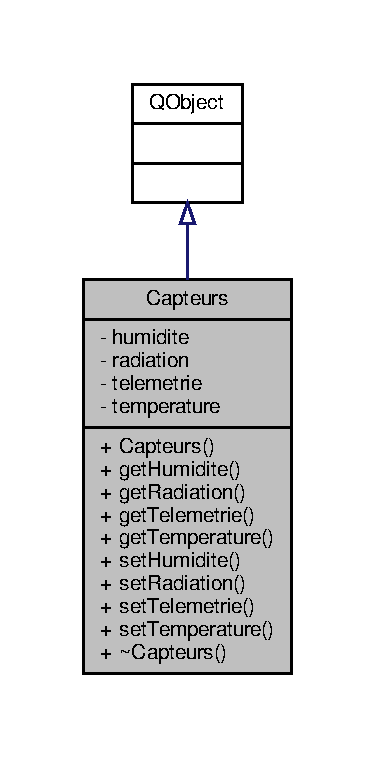
\includegraphics[width=180pt]{class_capteurs__coll__graph}
\end{center}
\end{figure}
\subsubsection*{Fonctions membres publiques}
\begin{DoxyCompactItemize}
\item 
\hyperlink{class_capteurs_a9d34c185400db797961c72498c48bbc0}{Capteurs} (\hyperlink{class_q_object}{Q\+Object} $\ast$parent=nullptr)
\begin{DoxyCompactList}\small\item\em Constructeur de la classe \hyperlink{class_capteurs}{Capteurs}. \end{DoxyCompactList}\item 
Q\+String \hyperlink{class_capteurs_a419b69b8b2fcc02a9bb7bdff39f87b06}{get\+Humidite} () const
\begin{DoxyCompactList}\small\item\em Récupère la dernière information issue du capteur de humidité \end{DoxyCompactList}\item 
Q\+String \hyperlink{class_capteurs_aaee3d64c752b09f8674fa62907f38cbc}{get\+Radiation} () const
\begin{DoxyCompactList}\small\item\em Récupère la dernière information issue du capteur de radiation. \end{DoxyCompactList}\item 
Q\+String \hyperlink{class_capteurs_ad8c2c486e92cc537dc014035b5634b60}{get\+Telemetrie} () const
\begin{DoxyCompactList}\small\item\em Récupère la dernière information issue du capteur télémétrique. \end{DoxyCompactList}\item 
Q\+String \hyperlink{class_capteurs_aa1346e5cbea9e37afc3694a0ea86bd99}{get\+Temperature} () const
\begin{DoxyCompactList}\small\item\em Récupère la dernière information issue du capteur de température. \end{DoxyCompactList}\item 
void \hyperlink{class_capteurs_aafb06e1746006cdb72e92dc7a0519a2e}{set\+Humidite} (Q\+String \hyperlink{class_capteurs_a8967c76dbc9c1f2ff8339cb8f00c3adb}{humidite})
\begin{DoxyCompactList}\small\item\em Modifie la dernière information issue du capteur de humidité \end{DoxyCompactList}\item 
void \hyperlink{class_capteurs_a8692d145188df3129d88fef77efbb7b0}{set\+Radiation} (Q\+String \hyperlink{class_capteurs_ad9d6f3fd6cc164c6cd5908fd7822f307}{radiation})
\begin{DoxyCompactList}\small\item\em Modifie la dernière information issue du capteur de radiation. \end{DoxyCompactList}\item 
void \hyperlink{class_capteurs_a399af986afb9d707138bc57a51e1f34f}{set\+Telemetrie} (Q\+String \hyperlink{class_capteurs_a336a4c4ad6ae1a49d21b265d2953e24b}{telemetrie})
\begin{DoxyCompactList}\small\item\em Modifie la dernière information issue du capteur télémétrique. \end{DoxyCompactList}\item 
void \hyperlink{class_capteurs_a8d6a0bceb4d236edf7b51335d9be8ecd}{set\+Temperature} (Q\+String \hyperlink{class_capteurs_acf6f97c1e121ae0f53c9a56430d42dfe}{temperature})
\begin{DoxyCompactList}\small\item\em Modifie la dernière information issue du capteur de température. \end{DoxyCompactList}\item 
\hyperlink{class_capteurs_a8d0e38fada71279279b2d3938485304b}{$\sim$\+Capteurs} ()
\begin{DoxyCompactList}\small\item\em Destructeur de la classe \hyperlink{class_capteurs}{Capteurs}. \end{DoxyCompactList}\end{DoxyCompactItemize}
\subsubsection*{Attributs privés}
\begin{DoxyCompactItemize}
\item 
Q\+String \hyperlink{class_capteurs_a8967c76dbc9c1f2ff8339cb8f00c3adb}{humidite}
\begin{DoxyCompactList}\small\item\em Dernière données de température. \end{DoxyCompactList}\item 
Q\+String \hyperlink{class_capteurs_ad9d6f3fd6cc164c6cd5908fd7822f307}{radiation}
\begin{DoxyCompactList}\small\item\em Dernière données de radiation. \end{DoxyCompactList}\item 
Q\+String \hyperlink{class_capteurs_a336a4c4ad6ae1a49d21b265d2953e24b}{telemetrie}
\begin{DoxyCompactList}\small\item\em Dernière données télémétriques. \end{DoxyCompactList}\item 
Q\+String \hyperlink{class_capteurs_acf6f97c1e121ae0f53c9a56430d42dfe}{temperature}
\begin{DoxyCompactList}\small\item\em Dernière données de température. \end{DoxyCompactList}\end{DoxyCompactItemize}


\subsubsection{Description détaillée}
Classe contenant les dernières informations issues des capteurs du rov. 

Définition à la ligne \hyperlink{capteurs_8h_source_l00018}{18} du fichier \hyperlink{capteurs_8h_source}{capteurs.\+h}.



\subsubsection{Documentation des constructeurs et destructeur}
\mbox{\Hypertarget{class_capteurs_a9d34c185400db797961c72498c48bbc0}\label{class_capteurs_a9d34c185400db797961c72498c48bbc0}} 
\index{Capteurs@{Capteurs}!Capteurs@{Capteurs}}
\index{Capteurs@{Capteurs}!Capteurs@{Capteurs}}
\paragraph{\texorpdfstring{Capteurs()}{Capteurs()}}
{\footnotesize\ttfamily Capteurs\+::\+Capteurs (\begin{DoxyParamCaption}\item[{\hyperlink{class_q_object}{Q\+Object} $\ast$}]{parent = {\ttfamily nullptr} }\end{DoxyParamCaption})}



Constructeur de la classe \hyperlink{class_capteurs}{Capteurs}. 


\begin{DoxyParams}{Paramètres}
{\em parent} & \\
\hline
\end{DoxyParams}


Définition à la ligne \hyperlink{capteurs_8cpp_source_l00009}{9} du fichier \hyperlink{capteurs_8cpp_source}{capteurs.\+cpp}.


\begin{DoxyCode}
00009                                   : \hyperlink{class_q_object}{QObject}(parent), \hyperlink{class_capteurs_a336a4c4ad6ae1a49d21b265d2953e24b}{telemetrie}(\textcolor{stringliteral}{"0"}), 
      \hyperlink{class_capteurs_acf6f97c1e121ae0f53c9a56430d42dfe}{temperature}(\textcolor{stringliteral}{"0"}), \hyperlink{class_capteurs_a8967c76dbc9c1f2ff8339cb8f00c3adb}{humidite}(\textcolor{stringliteral}{"0"}), \hyperlink{class_capteurs_ad9d6f3fd6cc164c6cd5908fd7822f307}{radiation}(\textcolor{stringliteral}{"0"})
00010 \{
00011     qDebug() << Q\_FUNC\_INFO;
00012 \}
\end{DoxyCode}
\mbox{\Hypertarget{class_capteurs_a8d0e38fada71279279b2d3938485304b}\label{class_capteurs_a8d0e38fada71279279b2d3938485304b}} 
\index{Capteurs@{Capteurs}!````~Capteurs@{$\sim$\+Capteurs}}
\index{````~Capteurs@{$\sim$\+Capteurs}!Capteurs@{Capteurs}}
\paragraph{\texorpdfstring{$\sim$\+Capteurs()}{~Capteurs()}}
{\footnotesize\ttfamily Capteurs\+::$\sim$\+Capteurs (\begin{DoxyParamCaption}{ }\end{DoxyParamCaption})}



Destructeur de la classe \hyperlink{class_capteurs}{Capteurs}. 



Définition à la ligne \hyperlink{capteurs_8cpp_source_l00014}{14} du fichier \hyperlink{capteurs_8cpp_source}{capteurs.\+cpp}.


\begin{DoxyCode}
00015 \{
00016     qDebug() << Q\_FUNC\_INFO;
00017 \}
\end{DoxyCode}


\subsubsection{Documentation des fonctions membres}
\mbox{\Hypertarget{class_capteurs_a419b69b8b2fcc02a9bb7bdff39f87b06}\label{class_capteurs_a419b69b8b2fcc02a9bb7bdff39f87b06}} 
\index{Capteurs@{Capteurs}!get\+Humidite@{get\+Humidite}}
\index{get\+Humidite@{get\+Humidite}!Capteurs@{Capteurs}}
\paragraph{\texorpdfstring{get\+Humidite()}{getHumidite()}}
{\footnotesize\ttfamily Q\+String Capteurs\+::get\+Humidite (\begin{DoxyParamCaption}{ }\end{DoxyParamCaption}) const}



Récupère la dernière information issue du capteur de humidité 

\begin{DoxyReturn}{Renvoie}
la dernière information issue du capteur de humidité 
\end{DoxyReturn}


Définition à la ligne \hyperlink{capteurs_8cpp_source_l00049}{49} du fichier \hyperlink{capteurs_8cpp_source}{capteurs.\+cpp}.



Références \hyperlink{capteurs_8h_source_l00024}{humidite}.


\begin{DoxyCode}
00050 \{
00051     \textcolor{keywordflow}{return} \hyperlink{class_capteurs_a8967c76dbc9c1f2ff8339cb8f00c3adb}{humidite};
00052 \}
\end{DoxyCode}
\mbox{\Hypertarget{class_capteurs_aaee3d64c752b09f8674fa62907f38cbc}\label{class_capteurs_aaee3d64c752b09f8674fa62907f38cbc}} 
\index{Capteurs@{Capteurs}!get\+Radiation@{get\+Radiation}}
\index{get\+Radiation@{get\+Radiation}!Capteurs@{Capteurs}}
\paragraph{\texorpdfstring{get\+Radiation()}{getRadiation()}}
{\footnotesize\ttfamily Q\+String Capteurs\+::get\+Radiation (\begin{DoxyParamCaption}{ }\end{DoxyParamCaption}) const}



Récupère la dernière information issue du capteur de radiation. 

\begin{DoxyReturn}{Renvoie}
la dernière information issue du capteur de radiation 
\end{DoxyReturn}


Définition à la ligne \hyperlink{capteurs_8cpp_source_l00054}{54} du fichier \hyperlink{capteurs_8cpp_source}{capteurs.\+cpp}.



Références \hyperlink{capteurs_8h_source_l00025}{radiation}.



Référencé par \hyperlink{ihmrov_8cpp_source_l00110}{I\+H\+M\+Rov\+::actualiser\+Informations()}.


\begin{DoxyCode}
00055 \{
00056     \textcolor{keywordflow}{return} \hyperlink{class_capteurs_ad9d6f3fd6cc164c6cd5908fd7822f307}{radiation};
00057 \}
\end{DoxyCode}
\mbox{\Hypertarget{class_capteurs_ad8c2c486e92cc537dc014035b5634b60}\label{class_capteurs_ad8c2c486e92cc537dc014035b5634b60}} 
\index{Capteurs@{Capteurs}!get\+Telemetrie@{get\+Telemetrie}}
\index{get\+Telemetrie@{get\+Telemetrie}!Capteurs@{Capteurs}}
\paragraph{\texorpdfstring{get\+Telemetrie()}{getTelemetrie()}}
{\footnotesize\ttfamily Q\+String Capteurs\+::get\+Telemetrie (\begin{DoxyParamCaption}{ }\end{DoxyParamCaption}) const}



Récupère la dernière information issue du capteur télémétrique. 

\begin{DoxyReturn}{Renvoie}
la dernière information issue du capteur télémétrique 
\end{DoxyReturn}


Définition à la ligne \hyperlink{capteurs_8cpp_source_l00039}{39} du fichier \hyperlink{capteurs_8cpp_source}{capteurs.\+cpp}.



Références \hyperlink{capteurs_8h_source_l00022}{telemetrie}.



Référencé par \hyperlink{ihmrov_8cpp_source_l00110}{I\+H\+M\+Rov\+::actualiser\+Informations()}.


\begin{DoxyCode}
00040 \{
00041     \textcolor{keywordflow}{return} \hyperlink{class_capteurs_a336a4c4ad6ae1a49d21b265d2953e24b}{telemetrie};
00042 \}
\end{DoxyCode}
\mbox{\Hypertarget{class_capteurs_aa1346e5cbea9e37afc3694a0ea86bd99}\label{class_capteurs_aa1346e5cbea9e37afc3694a0ea86bd99}} 
\index{Capteurs@{Capteurs}!get\+Temperature@{get\+Temperature}}
\index{get\+Temperature@{get\+Temperature}!Capteurs@{Capteurs}}
\paragraph{\texorpdfstring{get\+Temperature()}{getTemperature()}}
{\footnotesize\ttfamily Q\+String Capteurs\+::get\+Temperature (\begin{DoxyParamCaption}{ }\end{DoxyParamCaption}) const}



Récupère la dernière information issue du capteur de température. 

\begin{DoxyReturn}{Renvoie}
la dernière information issue du capteur de température 
\end{DoxyReturn}


Définition à la ligne \hyperlink{capteurs_8cpp_source_l00044}{44} du fichier \hyperlink{capteurs_8cpp_source}{capteurs.\+cpp}.



Références \hyperlink{capteurs_8h_source_l00023}{temperature}.



Référencé par \hyperlink{ihmrov_8cpp_source_l00110}{I\+H\+M\+Rov\+::actualiser\+Informations()}.


\begin{DoxyCode}
00045 \{
00046     \textcolor{keywordflow}{return} \hyperlink{class_capteurs_acf6f97c1e121ae0f53c9a56430d42dfe}{temperature};
00047 \}
\end{DoxyCode}
\mbox{\Hypertarget{class_capteurs_aafb06e1746006cdb72e92dc7a0519a2e}\label{class_capteurs_aafb06e1746006cdb72e92dc7a0519a2e}} 
\index{Capteurs@{Capteurs}!set\+Humidite@{set\+Humidite}}
\index{set\+Humidite@{set\+Humidite}!Capteurs@{Capteurs}}
\paragraph{\texorpdfstring{set\+Humidite()}{setHumidite()}}
{\footnotesize\ttfamily void Capteurs\+::set\+Humidite (\begin{DoxyParamCaption}\item[{Q\+String}]{humidite }\end{DoxyParamCaption})}



Modifie la dernière information issue du capteur de humidité 


\begin{DoxyParams}{Paramètres}
{\em humidite} & \\
\hline
\end{DoxyParams}


Définition à la ligne \hyperlink{capteurs_8cpp_source_l00029}{29} du fichier \hyperlink{capteurs_8cpp_source}{capteurs.\+cpp}.



Références \hyperlink{capteurs_8h_source_l00024}{humidite}.



Référencé par \hyperlink{rov_8cpp_source_l00086}{Rov\+::decoder\+Trame\+Capteur()}.


\begin{DoxyCode}
00030 \{
00031     this->\hyperlink{class_capteurs_a8967c76dbc9c1f2ff8339cb8f00c3adb}{humidite} = \hyperlink{class_capteurs_a8967c76dbc9c1f2ff8339cb8f00c3adb}{humidite};
00032 \}
\end{DoxyCode}
\mbox{\Hypertarget{class_capteurs_a8692d145188df3129d88fef77efbb7b0}\label{class_capteurs_a8692d145188df3129d88fef77efbb7b0}} 
\index{Capteurs@{Capteurs}!set\+Radiation@{set\+Radiation}}
\index{set\+Radiation@{set\+Radiation}!Capteurs@{Capteurs}}
\paragraph{\texorpdfstring{set\+Radiation()}{setRadiation()}}
{\footnotesize\ttfamily void Capteurs\+::set\+Radiation (\begin{DoxyParamCaption}\item[{Q\+String}]{radiation }\end{DoxyParamCaption})}



Modifie la dernière information issue du capteur de radiation. 


\begin{DoxyParams}{Paramètres}
{\em radiation} & \\
\hline
\end{DoxyParams}


Définition à la ligne \hyperlink{capteurs_8cpp_source_l00034}{34} du fichier \hyperlink{capteurs_8cpp_source}{capteurs.\+cpp}.



Références \hyperlink{capteurs_8h_source_l00025}{radiation}.



Référencé par \hyperlink{rov_8cpp_source_l00086}{Rov\+::decoder\+Trame\+Capteur()}.


\begin{DoxyCode}
00035 \{
00036     this->\hyperlink{class_capteurs_ad9d6f3fd6cc164c6cd5908fd7822f307}{radiation} = \hyperlink{class_capteurs_ad9d6f3fd6cc164c6cd5908fd7822f307}{radiation};
00037 \}
\end{DoxyCode}
\mbox{\Hypertarget{class_capteurs_a399af986afb9d707138bc57a51e1f34f}\label{class_capteurs_a399af986afb9d707138bc57a51e1f34f}} 
\index{Capteurs@{Capteurs}!set\+Telemetrie@{set\+Telemetrie}}
\index{set\+Telemetrie@{set\+Telemetrie}!Capteurs@{Capteurs}}
\paragraph{\texorpdfstring{set\+Telemetrie()}{setTelemetrie()}}
{\footnotesize\ttfamily void Capteurs\+::set\+Telemetrie (\begin{DoxyParamCaption}\item[{Q\+String}]{telemetrie }\end{DoxyParamCaption})}



Modifie la dernière information issue du capteur télémétrique. 


\begin{DoxyParams}{Paramètres}
{\em telemetrie} & \\
\hline
\end{DoxyParams}


Définition à la ligne \hyperlink{capteurs_8cpp_source_l00019}{19} du fichier \hyperlink{capteurs_8cpp_source}{capteurs.\+cpp}.



Références \hyperlink{capteurs_8h_source_l00022}{telemetrie}.



Référencé par \hyperlink{rov_8cpp_source_l00081}{Rov\+::decoder\+Trame\+Telemetrie()}.


\begin{DoxyCode}
00020 \{
00021     this->\hyperlink{class_capteurs_a336a4c4ad6ae1a49d21b265d2953e24b}{telemetrie} = \hyperlink{class_capteurs_a336a4c4ad6ae1a49d21b265d2953e24b}{telemetrie};
00022 \}
\end{DoxyCode}
\mbox{\Hypertarget{class_capteurs_a8d6a0bceb4d236edf7b51335d9be8ecd}\label{class_capteurs_a8d6a0bceb4d236edf7b51335d9be8ecd}} 
\index{Capteurs@{Capteurs}!set\+Temperature@{set\+Temperature}}
\index{set\+Temperature@{set\+Temperature}!Capteurs@{Capteurs}}
\paragraph{\texorpdfstring{set\+Temperature()}{setTemperature()}}
{\footnotesize\ttfamily void Capteurs\+::set\+Temperature (\begin{DoxyParamCaption}\item[{Q\+String}]{temperature }\end{DoxyParamCaption})}



Modifie la dernière information issue du capteur de température. 


\begin{DoxyParams}{Paramètres}
{\em temperature} & \\
\hline
\end{DoxyParams}


Définition à la ligne \hyperlink{capteurs_8cpp_source_l00024}{24} du fichier \hyperlink{capteurs_8cpp_source}{capteurs.\+cpp}.



Références \hyperlink{capteurs_8h_source_l00023}{temperature}.



Référencé par \hyperlink{rov_8cpp_source_l00086}{Rov\+::decoder\+Trame\+Capteur()}.


\begin{DoxyCode}
00025 \{
00026     this->\hyperlink{class_capteurs_acf6f97c1e121ae0f53c9a56430d42dfe}{temperature} = \hyperlink{class_capteurs_acf6f97c1e121ae0f53c9a56430d42dfe}{temperature};
00027 \}
\end{DoxyCode}


\subsubsection{Documentation des données membres}
\mbox{\Hypertarget{class_capteurs_a8967c76dbc9c1f2ff8339cb8f00c3adb}\label{class_capteurs_a8967c76dbc9c1f2ff8339cb8f00c3adb}} 
\index{Capteurs@{Capteurs}!humidite@{humidite}}
\index{humidite@{humidite}!Capteurs@{Capteurs}}
\paragraph{\texorpdfstring{humidite}{humidite}}
{\footnotesize\ttfamily Q\+String Capteurs\+::humidite\hspace{0.3cm}{\ttfamily [private]}}



Dernière données de température. 



Définition à la ligne \hyperlink{capteurs_8h_source_l00024}{24} du fichier \hyperlink{capteurs_8h_source}{capteurs.\+h}.



Référencé par \hyperlink{capteurs_8cpp_source_l00049}{get\+Humidite()}, et \hyperlink{capteurs_8cpp_source_l00029}{set\+Humidite()}.

\mbox{\Hypertarget{class_capteurs_ad9d6f3fd6cc164c6cd5908fd7822f307}\label{class_capteurs_ad9d6f3fd6cc164c6cd5908fd7822f307}} 
\index{Capteurs@{Capteurs}!radiation@{radiation}}
\index{radiation@{radiation}!Capteurs@{Capteurs}}
\paragraph{\texorpdfstring{radiation}{radiation}}
{\footnotesize\ttfamily Q\+String Capteurs\+::radiation\hspace{0.3cm}{\ttfamily [private]}}



Dernière données de radiation. 



Définition à la ligne \hyperlink{capteurs_8h_source_l00025}{25} du fichier \hyperlink{capteurs_8h_source}{capteurs.\+h}.



Référencé par \hyperlink{capteurs_8cpp_source_l00054}{get\+Radiation()}, et \hyperlink{capteurs_8cpp_source_l00034}{set\+Radiation()}.

\mbox{\Hypertarget{class_capteurs_a336a4c4ad6ae1a49d21b265d2953e24b}\label{class_capteurs_a336a4c4ad6ae1a49d21b265d2953e24b}} 
\index{Capteurs@{Capteurs}!telemetrie@{telemetrie}}
\index{telemetrie@{telemetrie}!Capteurs@{Capteurs}}
\paragraph{\texorpdfstring{telemetrie}{telemetrie}}
{\footnotesize\ttfamily Q\+String Capteurs\+::telemetrie\hspace{0.3cm}{\ttfamily [private]}}



Dernière données télémétriques. 



Définition à la ligne \hyperlink{capteurs_8h_source_l00022}{22} du fichier \hyperlink{capteurs_8h_source}{capteurs.\+h}.



Référencé par \hyperlink{capteurs_8cpp_source_l00039}{get\+Telemetrie()}, et \hyperlink{capteurs_8cpp_source_l00019}{set\+Telemetrie()}.

\mbox{\Hypertarget{class_capteurs_acf6f97c1e121ae0f53c9a56430d42dfe}\label{class_capteurs_acf6f97c1e121ae0f53c9a56430d42dfe}} 
\index{Capteurs@{Capteurs}!temperature@{temperature}}
\index{temperature@{temperature}!Capteurs@{Capteurs}}
\paragraph{\texorpdfstring{temperature}{temperature}}
{\footnotesize\ttfamily Q\+String Capteurs\+::temperature\hspace{0.3cm}{\ttfamily [private]}}



Dernière données de température. 



Définition à la ligne \hyperlink{capteurs_8h_source_l00023}{23} du fichier \hyperlink{capteurs_8h_source}{capteurs.\+h}.



Référencé par \hyperlink{capteurs_8cpp_source_l00044}{get\+Temperature()}, et \hyperlink{capteurs_8cpp_source_l00024}{set\+Temperature()}.



La documentation de cette classe a été générée à partir des fichiers suivants \+:\begin{DoxyCompactItemize}
\item 
\hyperlink{capteurs_8h}{capteurs.\+h}\item 
\hyperlink{capteurs_8cpp}{capteurs.\+cpp}\end{DoxyCompactItemize}

\hypertarget{class_communication_rov}{}\subsection{Référence de la classe Communication\+Rov}
\label{class_communication_rov}\index{Communication\+Rov@{Communication\+Rov}}


Class permettant de mettre en place une communication avec le rov.  




{\ttfamily \#include \char`\"{}communication\+Rov.\+h\char`\"{}}



Graphe de collaboration de Communication\+Rov\+:
\nopagebreak
\begin{figure}[H]
\begin{center}
\leavevmode
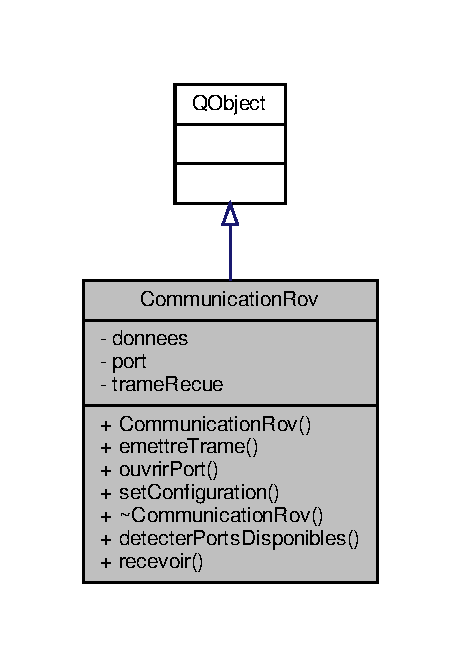
\includegraphics[width=221pt]{class_communication_rov__coll__graph}
\end{center}
\end{figure}
\subsubsection*{Connecteurs publics}
\begin{DoxyCompactItemize}
\item 
void \hyperlink{class_communication_rov_a75de69ca01c849f760d7efea1b2722b9}{recevoir} ()
\begin{DoxyCompactList}\small\item\em Récupere la trame disponible sur le port à la réception du signal Ready\+Read et émet un signal nouvelle\+Trame. \end{DoxyCompactList}\end{DoxyCompactItemize}
\subsubsection*{Signaux}
\begin{DoxyCompactItemize}
\item 
void \hyperlink{class_communication_rov_a78ee383e056cec7e8b24f3f9e472f60f}{nouvelle\+Trame} (Q\+String trame)
\begin{DoxyCompactList}\small\item\em Envoie un signal informant qu\textquotesingle{}une nouvelle trame est disponible. \end{DoxyCompactList}\end{DoxyCompactItemize}
\subsubsection*{Fonctions membres publiques}
\begin{DoxyCompactItemize}
\item 
\hyperlink{class_communication_rov_a22b64c69228d392a212f543e071adc02}{Communication\+Rov} (\hyperlink{class_q_object}{Q\+Object} $\ast$parent=nullptr)
\begin{DoxyCompactList}\small\item\em constructeur de la classe \hyperlink{class_communication_rov}{Communication\+Rov} \end{DoxyCompactList}\item 
int \hyperlink{class_communication_rov_a4f52076db8d6e78abe1745fa1e235272}{emettre\+Trame} (Q\+String trame)
\begin{DoxyCompactList}\small\item\em Emet la trame vers le robot. \end{DoxyCompactList}\item 
void \hyperlink{class_communication_rov_acc835a6d927b1b8cd631e64ffabca0b4}{ouvrir\+Port} ()
\begin{DoxyCompactList}\small\item\em Permet d\textquotesingle{}ouvrir le port série virtuel. \end{DoxyCompactList}\item 
void \hyperlink{class_communication_rov_a3d83702b8b9a753761d924556e55c38d}{set\+Configuration} (\hyperlink{struct_configuration}{Configuration} ma\+Configuration)
\begin{DoxyCompactList}\small\item\em Affecte a l\textquotesingle{}objet \hyperlink{class_communication_rov}{Communication\+Rov} une configuration du port série virtuel. \end{DoxyCompactList}\item 
\hyperlink{class_communication_rov_a97e96f47dad6d47cbec4adc82756b49e}{$\sim$\+Communication\+Rov} ()
\begin{DoxyCompactList}\small\item\em Destructeur de la classe \hyperlink{class_communication_rov}{Communication\+Rov}. \end{DoxyCompactList}\end{DoxyCompactItemize}
\subsubsection*{Fonctions membres publiques statiques}
\begin{DoxyCompactItemize}
\item 
static Q\+String\+List \hyperlink{class_communication_rov_ad9882c08083c66cd89b472b9244727e9}{detecter\+Ports\+Disponibles} ()
\end{DoxyCompactItemize}
\subsubsection*{Attributs privés}
\begin{DoxyCompactItemize}
\item 
Q\+Byte\+Array \hyperlink{class_communication_rov_acbb6939bb597179956c6f4bc5ca39f3f}{donnees}
\begin{DoxyCompactList}\small\item\em Tableau contenant les données bruts envoyé depuis la liason série. \end{DoxyCompactList}\item 
Q\+Serial\+Port $\ast$ \hyperlink{class_communication_rov_a21b62067ef0b2a6aec339df60b4abd72}{port}
\begin{DoxyCompactList}\small\item\em accède a la configuration de la liaison série \end{DoxyCompactList}\item 
Q\+String \hyperlink{class_communication_rov_a2f5a49875a9fa51800522c531ecc65fc}{trame\+Recue}
\begin{DoxyCompactList}\small\item\em Derniere trame\+Recue. \end{DoxyCompactList}\end{DoxyCompactItemize}


\subsubsection{Description détaillée}
Class permettant de mettre en place une communication avec le rov. 

Définition à la ligne \hyperlink{communicationrov_8h_source_l00038}{38} du fichier \hyperlink{communicationrov_8h_source}{communicationrov.\+h}.



\subsubsection{Documentation des constructeurs et destructeur}
\mbox{\Hypertarget{class_communication_rov_a22b64c69228d392a212f543e071adc02}\label{class_communication_rov_a22b64c69228d392a212f543e071adc02}} 
\index{Communication\+Rov@{Communication\+Rov}!Communication\+Rov@{Communication\+Rov}}
\index{Communication\+Rov@{Communication\+Rov}!Communication\+Rov@{Communication\+Rov}}
\paragraph{\texorpdfstring{Communication\+Rov()}{CommunicationRov()}}
{\footnotesize\ttfamily Communication\+Rov\+::\+Communication\+Rov (\begin{DoxyParamCaption}\item[{\hyperlink{class_q_object}{Q\+Object} $\ast$}]{parent = {\ttfamily nullptr} }\end{DoxyParamCaption})}



constructeur de la classe \hyperlink{class_communication_rov}{Communication\+Rov} 


\begin{DoxyParams}{Paramètres}
{\em parent} & \\
\hline
\end{DoxyParams}


Définition à la ligne \hyperlink{communicationrov_8cpp_source_l00009}{9} du fichier \hyperlink{communicationrov_8cpp_source}{communicationrov.\+cpp}.



Références \hyperlink{communicationrov_8cpp_source_l00037}{ouvrir\+Port()}, et \hyperlink{communicationrov_8h_source_l00042}{port}.


\begin{DoxyCode}
00009                                                   : \hyperlink{class_q_object}{QObject}(parent)
00010 \{
00011     qDebug() << Q\_FUNC\_INFO;
00012     \hyperlink{class_communication_rov_a21b62067ef0b2a6aec339df60b4abd72}{port} = \textcolor{keyword}{new} QSerialPort(\textcolor{keyword}{this});
00013 
00014 \textcolor{preprocessor}{    #ifdef CONFIGURATION\_MANUELLE}
00015         \hyperlink{class_communication_rov_a21b62067ef0b2a6aec339df60b4abd72}{port}->setPortName(\textcolor{stringliteral}{"/dev/ttyUSB0"});
00016         \hyperlink{class_communication_rov_a21b62067ef0b2a6aec339df60b4abd72}{port}->setBaudRate(QSerialPort::Baud115200);
00017         \hyperlink{class_communication_rov_a21b62067ef0b2a6aec339df60b4abd72}{port}->setDataBits(QSerialPort::Data8);
00018         \hyperlink{class_communication_rov_a21b62067ef0b2a6aec339df60b4abd72}{port}->setStopBits(QSerialPort::OneStop);
00019         \hyperlink{class_communication_rov_a21b62067ef0b2a6aec339df60b4abd72}{port}->setParity(QSerialPort::NoParity);
00020         \hyperlink{class_communication_rov_a21b62067ef0b2a6aec339df60b4abd72}{port}->setFlowControl(QSerialPort::NoFlowControl);
00021 
00022         \hyperlink{class_communication_rov_acc835a6d927b1b8cd631e64ffabca0b4}{ouvrirPort}();
00023 \textcolor{preprocessor}{    #else}
00024 
00027 \textcolor{preprocessor}{    #endif}
00028 \}
\end{DoxyCode}
\mbox{\Hypertarget{class_communication_rov_a97e96f47dad6d47cbec4adc82756b49e}\label{class_communication_rov_a97e96f47dad6d47cbec4adc82756b49e}} 
\index{Communication\+Rov@{Communication\+Rov}!````~Communication\+Rov@{$\sim$\+Communication\+Rov}}
\index{````~Communication\+Rov@{$\sim$\+Communication\+Rov}!Communication\+Rov@{Communication\+Rov}}
\paragraph{\texorpdfstring{$\sim$\+Communication\+Rov()}{~CommunicationRov()}}
{\footnotesize\ttfamily Communication\+Rov\+::$\sim$\+Communication\+Rov (\begin{DoxyParamCaption}{ }\end{DoxyParamCaption})}



Destructeur de la classe \hyperlink{class_communication_rov}{Communication\+Rov}. 



Définition à la ligne \hyperlink{communicationrov_8cpp_source_l00030}{30} du fichier \hyperlink{communicationrov_8cpp_source}{communicationrov.\+cpp}.



Références \hyperlink{communicationrov_8h_source_l00042}{port}.


\begin{DoxyCode}
00031 \{
00032     \textcolor{keywordflow}{if}(\hyperlink{class_communication_rov_a21b62067ef0b2a6aec339df60b4abd72}{port}->isOpen())
00033         \hyperlink{class_communication_rov_a21b62067ef0b2a6aec339df60b4abd72}{port}->close();
00034     qDebug() << Q\_FUNC\_INFO;
00035 \}
\end{DoxyCode}


\subsubsection{Documentation des fonctions membres}
\mbox{\Hypertarget{class_communication_rov_ad9882c08083c66cd89b472b9244727e9}\label{class_communication_rov_ad9882c08083c66cd89b472b9244727e9}} 
\index{Communication\+Rov@{Communication\+Rov}!detecter\+Ports\+Disponibles@{detecter\+Ports\+Disponibles}}
\index{detecter\+Ports\+Disponibles@{detecter\+Ports\+Disponibles}!Communication\+Rov@{Communication\+Rov}}
\paragraph{\texorpdfstring{detecter\+Ports\+Disponibles()}{detecterPortsDisponibles()}}
{\footnotesize\ttfamily Q\+String\+List Communication\+Rov\+::detecter\+Ports\+Disponibles (\begin{DoxyParamCaption}{ }\end{DoxyParamCaption})\hspace{0.3cm}{\ttfamily [static]}}



Définition à la ligne \hyperlink{communicationrov_8cpp_source_l00090}{90} du fichier \hyperlink{communicationrov_8cpp_source}{communicationrov.\+cpp}.



Référencé par \hyperlink{ihmconfiguration_8cpp_source_l00033}{I\+H\+M\+Configuration\+::configurer\+Widgets()}.


\begin{DoxyCode}
00091 \{
00092     QStringList listePortsDetectes;
00093 
00094     \textcolor{keywordflow}{foreach}(\textcolor{keyword}{const} QSerialPortInfo &info, QSerialPortInfo::availablePorts())
00095     \{
00096         listePortsDetectes.push\_back(info.portName());
00097     \}
00098 
00099     \textcolor{keywordflow}{return} listePortsDetectes;
00100 \}
\end{DoxyCode}
\mbox{\Hypertarget{class_communication_rov_a4f52076db8d6e78abe1745fa1e235272}\label{class_communication_rov_a4f52076db8d6e78abe1745fa1e235272}} 
\index{Communication\+Rov@{Communication\+Rov}!emettre\+Trame@{emettre\+Trame}}
\index{emettre\+Trame@{emettre\+Trame}!Communication\+Rov@{Communication\+Rov}}
\paragraph{\texorpdfstring{emettre\+Trame()}{emettreTrame()}}
{\footnotesize\ttfamily int Communication\+Rov\+::emettre\+Trame (\begin{DoxyParamCaption}\item[{Q\+String}]{trame }\end{DoxyParamCaption})}



Emet la trame vers le robot. 


\begin{DoxyParams}{Paramètres}
{\em trame} & \\
\hline
\end{DoxyParams}
\begin{DoxyReturn}{Renvoie}
un entier correspondant au nombres d\textquotesingle{}octets envoyé, retourne -\/1 si la diffusion à échoué 
\end{DoxyReturn}


Définition à la ligne \hyperlink{communicationrov_8cpp_source_l00060}{60} du fichier \hyperlink{communicationrov_8cpp_source}{communicationrov.\+cpp}.



Références \hyperlink{communicationrov_8h_source_l00042}{port}.



Référencé par \hyperlink{rov_8cpp_source_l00251}{Rov\+::creer\+Trame\+Camera()}, \hyperlink{rov_8cpp_source_l00208}{Rov\+::creer\+Trame\+Deplacement()}, \hyperlink{rov_8cpp_source_l00230}{Rov\+::creer\+Trame\+Ordre()}, \hyperlink{rov_8cpp_source_l00219}{Rov\+::creer\+Trame\+Pilotage()}, et \hyperlink{rov_8cpp_source_l00240}{Rov\+::creer\+Trame\+Pince()}.


\begin{DoxyCode}
00061 \{
00062     \textcolor{keywordtype}{int} nombresOctets = -1;
00063 
00064     \textcolor{keywordflow}{if} (\hyperlink{class_communication_rov_a21b62067ef0b2a6aec339df60b4abd72}{port} == NULL || !\hyperlink{class_communication_rov_a21b62067ef0b2a6aec339df60b4abd72}{port}->isOpen())
00065     \{
00066        \textcolor{keywordflow}{return} -1;
00067     \}
00068 
00069     nombresOctets = \hyperlink{class_communication_rov_a21b62067ef0b2a6aec339df60b4abd72}{port}->write(trame.toLatin1());
00070     \textcolor{keywordflow}{return} nombresOctets;
00071 \}
\end{DoxyCode}
\mbox{\Hypertarget{class_communication_rov_a78ee383e056cec7e8b24f3f9e472f60f}\label{class_communication_rov_a78ee383e056cec7e8b24f3f9e472f60f}} 
\index{Communication\+Rov@{Communication\+Rov}!nouvelle\+Trame@{nouvelle\+Trame}}
\index{nouvelle\+Trame@{nouvelle\+Trame}!Communication\+Rov@{Communication\+Rov}}
\paragraph{\texorpdfstring{nouvelle\+Trame}{nouvelleTrame}}
{\footnotesize\ttfamily void Communication\+Rov\+::nouvelle\+Trame (\begin{DoxyParamCaption}\item[{Q\+String}]{trame }\end{DoxyParamCaption})\hspace{0.3cm}{\ttfamily [signal]}}



Envoie un signal informant qu\textquotesingle{}une nouvelle trame est disponible. 


\begin{DoxyParams}{Paramètres}
{\em trame} & \\
\hline
\end{DoxyParams}


Référencé par \hyperlink{communicationrov_8cpp_source_l00073}{recevoir()}.

\mbox{\Hypertarget{class_communication_rov_acc835a6d927b1b8cd631e64ffabca0b4}\label{class_communication_rov_acc835a6d927b1b8cd631e64ffabca0b4}} 
\index{Communication\+Rov@{Communication\+Rov}!ouvrir\+Port@{ouvrir\+Port}}
\index{ouvrir\+Port@{ouvrir\+Port}!Communication\+Rov@{Communication\+Rov}}
\paragraph{\texorpdfstring{ouvrir\+Port()}{ouvrirPort()}}
{\footnotesize\ttfamily void Communication\+Rov\+::ouvrir\+Port (\begin{DoxyParamCaption}{ }\end{DoxyParamCaption})}



Permet d\textquotesingle{}ouvrir le port série virtuel. 



Définition à la ligne \hyperlink{communicationrov_8cpp_source_l00037}{37} du fichier \hyperlink{communicationrov_8cpp_source}{communicationrov.\+cpp}.



Références \hyperlink{communicationrov_8h_source_l00042}{port}, et \hyperlink{communicationrov_8cpp_source_l00073}{recevoir()}.



Référencé par \hyperlink{communicationrov_8cpp_source_l00009}{Communication\+Rov()}.


\begin{DoxyCode}
00038 \{
00039     \textcolor{keywordflow}{if}(\hyperlink{class_communication_rov_a21b62067ef0b2a6aec339df60b4abd72}{port}->open(QIODevice::ReadWrite))
00040     \{
00041         \textcolor{keywordflow}{if}(\hyperlink{class_communication_rov_a21b62067ef0b2a6aec339df60b4abd72}{port}->isOpen())
00042             connect(\hyperlink{class_communication_rov_a21b62067ef0b2a6aec339df60b4abd72}{port}, SIGNAL(readyRead()), \textcolor{keyword}{this}, SLOT(\hyperlink{class_communication_rov_a75de69ca01c849f760d7efea1b2722b9}{recevoir}()));
00043     \}
00044 \textcolor{preprocessor}{    #ifdef MODE\_CONNECTE}
00045     \textcolor{keywordflow}{else}
00046         QMessageBox::critical(\textcolor{keyword}{nullptr}, \textcolor{stringliteral}{"Communication rov"}, QString::fromUtf8(\textcolor{stringliteral}{"Erreur ouverture du port
       série !"}));
00047 \textcolor{preprocessor}{    #endif}
00048 \}
\end{DoxyCode}
\mbox{\Hypertarget{class_communication_rov_a75de69ca01c849f760d7efea1b2722b9}\label{class_communication_rov_a75de69ca01c849f760d7efea1b2722b9}} 
\index{Communication\+Rov@{Communication\+Rov}!recevoir@{recevoir}}
\index{recevoir@{recevoir}!Communication\+Rov@{Communication\+Rov}}
\paragraph{\texorpdfstring{recevoir}{recevoir}}
{\footnotesize\ttfamily void Communication\+Rov\+::recevoir (\begin{DoxyParamCaption}{ }\end{DoxyParamCaption})\hspace{0.3cm}{\ttfamily [slot]}}



Récupere la trame disponible sur le port à la réception du signal Ready\+Read et émet un signal nouvelle\+Trame. 



Définition à la ligne \hyperlink{communicationrov_8cpp_source_l00073}{73} du fichier \hyperlink{communicationrov_8cpp_source}{communicationrov.\+cpp}.



Références \hyperlink{communicationrov_8h_source_l00043}{donnees}, \hyperlink{class_communication_rov_a78ee383e056cec7e8b24f3f9e472f60f}{nouvelle\+Trame()}, \hyperlink{communicationrov_8h_source_l00042}{port}, et \hyperlink{communicationrov_8h_source_l00044}{trame\+Recue}.



Référencé par \hyperlink{communicationrov_8cpp_source_l00037}{ouvrir\+Port()}.


\begin{DoxyCode}
00074 \{
00075     \textcolor{keywordflow}{while}(\hyperlink{class_communication_rov_a21b62067ef0b2a6aec339df60b4abd72}{port}->bytesAvailable())
00076     \{
00077         \hyperlink{class_communication_rov_acbb6939bb597179956c6f4bc5ca39f3f}{donnees} += \hyperlink{class_communication_rov_a21b62067ef0b2a6aec339df60b4abd72}{port}->readAll();
00078         qDebug() << Q\_FUNC\_INFO << \textcolor{stringliteral}{"bytesAvailable"} << \hyperlink{class_communication_rov_a21b62067ef0b2a6aec339df60b4abd72}{port}->bytesAvailable() << \textcolor{stringliteral}{"donnees"} << 
      \hyperlink{class_communication_rov_acbb6939bb597179956c6f4bc5ca39f3f}{donnees};
00079     \}
00080 
00081     \textcolor{keywordflow}{if}(\hyperlink{class_communication_rov_acbb6939bb597179956c6f4bc5ca39f3f}{donnees}.startsWith(\textcolor{stringliteral}{"$"}) && \hyperlink{class_communication_rov_acbb6939bb597179956c6f4bc5ca39f3f}{donnees}.endsWith(\textcolor{stringliteral}{"\(\backslash\)r\(\backslash\)n"}))
00082     \{
00083         \hyperlink{class_communication_rov_a2f5a49875a9fa51800522c531ecc65fc}{trameRecue} = QString(\hyperlink{class_communication_rov_acbb6939bb597179956c6f4bc5ca39f3f}{donnees}.data());
00084         qDebug() << Q\_FUNC\_INFO << \textcolor{stringliteral}{"trameRecue"} << \hyperlink{class_communication_rov_a2f5a49875a9fa51800522c531ecc65fc}{trameRecue};
00085         emit \hyperlink{class_communication_rov_a78ee383e056cec7e8b24f3f9e472f60f}{nouvelleTrame}(trameRecue);
00086         \hyperlink{class_communication_rov_acbb6939bb597179956c6f4bc5ca39f3f}{donnees}.clear();
00087     \}
00088 \}
\end{DoxyCode}
\mbox{\Hypertarget{class_communication_rov_a3d83702b8b9a753761d924556e55c38d}\label{class_communication_rov_a3d83702b8b9a753761d924556e55c38d}} 
\index{Communication\+Rov@{Communication\+Rov}!set\+Configuration@{set\+Configuration}}
\index{set\+Configuration@{set\+Configuration}!Communication\+Rov@{Communication\+Rov}}
\paragraph{\texorpdfstring{set\+Configuration()}{setConfiguration()}}
{\footnotesize\ttfamily void Communication\+Rov\+::set\+Configuration (\begin{DoxyParamCaption}\item[{\hyperlink{struct_configuration}{Configuration}}]{ma\+Configuration }\end{DoxyParamCaption})}



Affecte a l\textquotesingle{}objet \hyperlink{class_communication_rov}{Communication\+Rov} une configuration du port série virtuel. 


\begin{DoxyParams}{Paramètres}
{\em ma\+Configuration} & \\
\hline
\end{DoxyParams}


Définition à la ligne \hyperlink{communicationrov_8cpp_source_l00050}{50} du fichier \hyperlink{communicationrov_8cpp_source}{communicationrov.\+cpp}.



Références \hyperlink{communicationrov_8h_source_l00028}{Configuration\+::bits\+Donnees}, \hyperlink{communicationrov_8h_source_l00029}{Configuration\+::bit\+Stop}, \hyperlink{communicationrov_8h_source_l00027}{Configuration\+::debit}, \hyperlink{communicationrov_8h_source_l00026}{Configuration\+::port}, et \hyperlink{communicationrov_8h_source_l00042}{port}.


\begin{DoxyCode}
00051 \{
00052     \hyperlink{class_communication_rov_a21b62067ef0b2a6aec339df60b4abd72}{port}->setPortName(maConfiguration.\hyperlink{struct_configuration_acc40b4f298cb215a94fb43976ef7d3a8}{port});
00053     \hyperlink{class_communication_rov_a21b62067ef0b2a6aec339df60b4abd72}{port}->setBaudRate(maConfiguration.\hyperlink{struct_configuration_ab714d6036189bf451e566e6c6a971c85}{debit});
00054     \hyperlink{class_communication_rov_a21b62067ef0b2a6aec339df60b4abd72}{port}->setDataBits((QSerialPort::DataBits)maConfiguration.\hyperlink{struct_configuration_a37e0691e4a25b11bd86a52bc68c81f93}{bitsDonnees});
00055     \hyperlink{class_communication_rov_a21b62067ef0b2a6aec339df60b4abd72}{port}->setStopBits((QSerialPort::StopBits)maConfiguration.\hyperlink{struct_configuration_a9c24ff9a3e5a24b14e1ac8bc03de907d}{bitStop});
00056     \hyperlink{class_communication_rov_a21b62067ef0b2a6aec339df60b4abd72}{port}->setParity(QSerialPort::NoParity);
00057     \hyperlink{class_communication_rov_a21b62067ef0b2a6aec339df60b4abd72}{port}->setFlowControl(QSerialPort::NoFlowControl);
00058 \}
\end{DoxyCode}


\subsubsection{Documentation des données membres}
\mbox{\Hypertarget{class_communication_rov_acbb6939bb597179956c6f4bc5ca39f3f}\label{class_communication_rov_acbb6939bb597179956c6f4bc5ca39f3f}} 
\index{Communication\+Rov@{Communication\+Rov}!donnees@{donnees}}
\index{donnees@{donnees}!Communication\+Rov@{Communication\+Rov}}
\paragraph{\texorpdfstring{donnees}{donnees}}
{\footnotesize\ttfamily Q\+Byte\+Array Communication\+Rov\+::donnees\hspace{0.3cm}{\ttfamily [private]}}



Tableau contenant les données bruts envoyé depuis la liason série. 



Définition à la ligne \hyperlink{communicationrov_8h_source_l00043}{43} du fichier \hyperlink{communicationrov_8h_source}{communicationrov.\+h}.



Référencé par \hyperlink{communicationrov_8cpp_source_l00073}{recevoir()}.

\mbox{\Hypertarget{class_communication_rov_a21b62067ef0b2a6aec339df60b4abd72}\label{class_communication_rov_a21b62067ef0b2a6aec339df60b4abd72}} 
\index{Communication\+Rov@{Communication\+Rov}!port@{port}}
\index{port@{port}!Communication\+Rov@{Communication\+Rov}}
\paragraph{\texorpdfstring{port}{port}}
{\footnotesize\ttfamily Q\+Serial\+Port$\ast$ Communication\+Rov\+::port\hspace{0.3cm}{\ttfamily [private]}}



accède a la configuration de la liaison série 



Définition à la ligne \hyperlink{communicationrov_8h_source_l00042}{42} du fichier \hyperlink{communicationrov_8h_source}{communicationrov.\+h}.



Référencé par \hyperlink{communicationrov_8cpp_source_l00009}{Communication\+Rov()}, \hyperlink{communicationrov_8cpp_source_l00060}{emettre\+Trame()}, \hyperlink{communicationrov_8cpp_source_l00037}{ouvrir\+Port()}, \hyperlink{communicationrov_8cpp_source_l00073}{recevoir()}, \hyperlink{communicationrov_8cpp_source_l00050}{set\+Configuration()}, et \hyperlink{communicationrov_8cpp_source_l00030}{$\sim$\+Communication\+Rov()}.

\mbox{\Hypertarget{class_communication_rov_a2f5a49875a9fa51800522c531ecc65fc}\label{class_communication_rov_a2f5a49875a9fa51800522c531ecc65fc}} 
\index{Communication\+Rov@{Communication\+Rov}!trame\+Recue@{trame\+Recue}}
\index{trame\+Recue@{trame\+Recue}!Communication\+Rov@{Communication\+Rov}}
\paragraph{\texorpdfstring{trame\+Recue}{trameRecue}}
{\footnotesize\ttfamily Q\+String Communication\+Rov\+::trame\+Recue\hspace{0.3cm}{\ttfamily [private]}}



Derniere trame\+Recue. 



Définition à la ligne \hyperlink{communicationrov_8h_source_l00044}{44} du fichier \hyperlink{communicationrov_8h_source}{communicationrov.\+h}.



Référencé par \hyperlink{communicationrov_8cpp_source_l00073}{recevoir()}.



La documentation de cette classe a été générée à partir des fichiers suivants \+:\begin{DoxyCompactItemize}
\item 
\hyperlink{communicationrov_8h}{communicationrov.\+h}\item 
\hyperlink{communicationrov_8cpp}{communicationrov.\+cpp}\end{DoxyCompactItemize}

\hypertarget{struct_configuration}{}\subsection{Référence de la structure Configuration}
\label{struct_configuration}\index{Configuration@{Configuration}}


structure permettant de configurer une communication  




{\ttfamily \#include $<$communicationrov.\+h$>$}



Graphe de collaboration de Configuration\+:\nopagebreak
\begin{figure}[H]
\begin{center}
\leavevmode
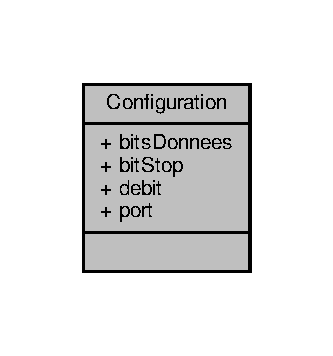
\includegraphics[width=160pt]{struct_configuration__coll__graph}
\end{center}
\end{figure}
\subsubsection*{Attributs publics}
\begin{DoxyCompactItemize}
\item 
int \hyperlink{struct_configuration_a37e0691e4a25b11bd86a52bc68c81f93}{bits\+Donnees}
\begin{DoxyCompactList}\small\item\em Attribut définissant le nombre de bits de données de la communication. \end{DoxyCompactList}\item 
int \hyperlink{struct_configuration_a9c24ff9a3e5a24b14e1ac8bc03de907d}{bit\+Stop}
\begin{DoxyCompactList}\small\item\em Attribut définissant le nombre de bits de stop de la communication. \end{DoxyCompactList}\item 
int \hyperlink{struct_configuration_ab714d6036189bf451e566e6c6a971c85}{debit}
\begin{DoxyCompactList}\small\item\em Attribut définissant la vitesse en bits/s de la communication. \end{DoxyCompactList}\item 
Q\+String \hyperlink{struct_configuration_acc40b4f298cb215a94fb43976ef7d3a8}{port}
\begin{DoxyCompactList}\small\item\em Attribut définissant le nom d\textquotesingle{}un port. \end{DoxyCompactList}\end{DoxyCompactItemize}


\subsubsection{Description détaillée}
structure permettant de configurer une communication 

Définition à la ligne \hyperlink{communicationrov_8h_source_l00024}{24} du fichier \hyperlink{communicationrov_8h_source}{communicationrov.\+h}.



\subsubsection{Documentation des données membres}
\mbox{\Hypertarget{struct_configuration_a37e0691e4a25b11bd86a52bc68c81f93}\label{struct_configuration_a37e0691e4a25b11bd86a52bc68c81f93}} 
\index{Configuration@{Configuration}!bits\+Donnees@{bits\+Donnees}}
\index{bits\+Donnees@{bits\+Donnees}!Configuration@{Configuration}}
\paragraph{\texorpdfstring{bits\+Donnees}{bitsDonnees}}
{\footnotesize\ttfamily int Configuration\+::bits\+Donnees}



Attribut définissant le nombre de bits de données de la communication. 



Définition à la ligne \hyperlink{communicationrov_8h_source_l00028}{28} du fichier \hyperlink{communicationrov_8h_source}{communicationrov.\+h}.



Référencé par \hyperlink{communicationrov_8cpp_source_l00050}{Communication\+Rov\+::set\+Configuration()}.

\mbox{\Hypertarget{struct_configuration_a9c24ff9a3e5a24b14e1ac8bc03de907d}\label{struct_configuration_a9c24ff9a3e5a24b14e1ac8bc03de907d}} 
\index{Configuration@{Configuration}!bit\+Stop@{bit\+Stop}}
\index{bit\+Stop@{bit\+Stop}!Configuration@{Configuration}}
\paragraph{\texorpdfstring{bit\+Stop}{bitStop}}
{\footnotesize\ttfamily int Configuration\+::bit\+Stop}



Attribut définissant le nombre de bits de stop de la communication. 



Définition à la ligne \hyperlink{communicationrov_8h_source_l00029}{29} du fichier \hyperlink{communicationrov_8h_source}{communicationrov.\+h}.



Référencé par \hyperlink{communicationrov_8cpp_source_l00050}{Communication\+Rov\+::set\+Configuration()}.

\mbox{\Hypertarget{struct_configuration_ab714d6036189bf451e566e6c6a971c85}\label{struct_configuration_ab714d6036189bf451e566e6c6a971c85}} 
\index{Configuration@{Configuration}!debit@{debit}}
\index{debit@{debit}!Configuration@{Configuration}}
\paragraph{\texorpdfstring{debit}{debit}}
{\footnotesize\ttfamily int Configuration\+::debit}



Attribut définissant la vitesse en bits/s de la communication. 



Définition à la ligne \hyperlink{communicationrov_8h_source_l00027}{27} du fichier \hyperlink{communicationrov_8h_source}{communicationrov.\+h}.



Référencé par \hyperlink{communicationrov_8cpp_source_l00050}{Communication\+Rov\+::set\+Configuration()}.

\mbox{\Hypertarget{struct_configuration_acc40b4f298cb215a94fb43976ef7d3a8}\label{struct_configuration_acc40b4f298cb215a94fb43976ef7d3a8}} 
\index{Configuration@{Configuration}!port@{port}}
\index{port@{port}!Configuration@{Configuration}}
\paragraph{\texorpdfstring{port}{port}}
{\footnotesize\ttfamily Q\+String Configuration\+::port}



Attribut définissant le nom d\textquotesingle{}un port. 



Définition à la ligne \hyperlink{communicationrov_8h_source_l00026}{26} du fichier \hyperlink{communicationrov_8h_source}{communicationrov.\+h}.



Référencé par \hyperlink{communicationrov_8cpp_source_l00050}{Communication\+Rov\+::set\+Configuration()}.



La documentation de cette structure a été générée à partir du fichier suivant \+:\begin{DoxyCompactItemize}
\item 
\hyperlink{communicationrov_8h}{communicationrov.\+h}\end{DoxyCompactItemize}

\hypertarget{struct_etat_manette_bouton}{}\subsection{Référence de la structure Etat\+Manette\+Bouton}
\label{struct_etat_manette_bouton}\index{Etat\+Manette\+Bouton@{Etat\+Manette\+Bouton}}


Structure qui définit l\textquotesingle{}état de la manette en mode pilotage de la pince.  




{\ttfamily \#include $<$manette.\+h$>$}



Graphe de collaboration de Etat\+Manette\+Bouton\+:\nopagebreak
\begin{figure}[H]
\begin{center}
\leavevmode
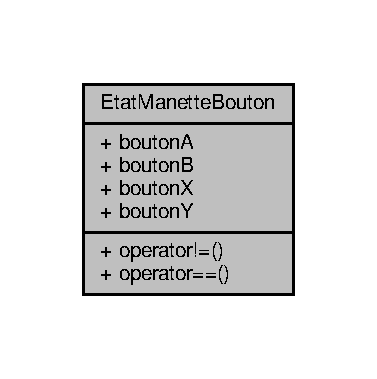
\includegraphics[width=181pt]{struct_etat_manette_bouton__coll__graph}
\end{center}
\end{figure}
\subsubsection*{Fonctions membres publiques}
\begin{DoxyCompactItemize}
\item 
bool \hyperlink{struct_etat_manette_bouton_a6ebd196e0fe68d30a8238b3e12194c93}{operator!=} (const \hyperlink{struct_etat_manette_bouton}{Etat\+Manette\+Bouton} \&ma\+Structure) const
\begin{DoxyCompactList}\small\item\em Surcharge de l\textquotesingle{}opérateur != afin de comparer un état de manette prédéfini avec l\textquotesingle{}état actuel de la manette. \end{DoxyCompactList}\item 
bool \hyperlink{struct_etat_manette_bouton_a7898661d3d19b6d8cf7005111d670ede}{operator==} (const \hyperlink{struct_etat_manette_bouton}{Etat\+Manette\+Bouton} \&ma\+Structure) const
\begin{DoxyCompactList}\small\item\em Surcharge de l\textquotesingle{}opérateur == afin de comparer un état de manette prédéfini avec l\textquotesingle{}état actuel de la manette. \end{DoxyCompactList}\end{DoxyCompactItemize}
\subsubsection*{Attributs publics}
\begin{DoxyCompactItemize}
\item 
bool \hyperlink{struct_etat_manette_bouton_a0a1bcb57b5ce1a3f4ff6de5e8749c052}{boutonA}
\begin{DoxyCompactList}\small\item\em Membre définissant l\textquotesingle{}état du bouton A. \end{DoxyCompactList}\item 
bool \hyperlink{struct_etat_manette_bouton_a2a0f4d809b1b9b814fa689113becaad7}{boutonB}
\begin{DoxyCompactList}\small\item\em Membre définissant l\textquotesingle{}état du bouton B. \end{DoxyCompactList}\item 
bool \hyperlink{struct_etat_manette_bouton_a4a1d74300413624fd13841eb11c6e974}{boutonX}
\begin{DoxyCompactList}\small\item\em Membre définissant l\textquotesingle{}état du bouton X. \end{DoxyCompactList}\item 
bool \hyperlink{struct_etat_manette_bouton_aae061f9e32f970787226ef9e0bdb5a17}{boutonY}
\begin{DoxyCompactList}\small\item\em Membre définissant l\textquotesingle{}état du bouton Y. \end{DoxyCompactList}\end{DoxyCompactItemize}


\subsubsection{Description détaillée}
Structure qui définit l\textquotesingle{}état de la manette en mode pilotage de la pince. 

Définition à la ligne \hyperlink{manette_8h_source_l00122}{122} du fichier \hyperlink{manette_8h_source}{manette.\+h}.



\subsubsection{Documentation des fonctions membres}
\mbox{\Hypertarget{struct_etat_manette_bouton_a6ebd196e0fe68d30a8238b3e12194c93}\label{struct_etat_manette_bouton_a6ebd196e0fe68d30a8238b3e12194c93}} 
\index{Etat\+Manette\+Bouton@{Etat\+Manette\+Bouton}!operator"!=@{operator"!=}}
\index{operator"!=@{operator"!=}!Etat\+Manette\+Bouton@{Etat\+Manette\+Bouton}}
\paragraph{\texorpdfstring{operator"!=()}{operator!=()}}
{\footnotesize\ttfamily bool Etat\+Manette\+Bouton\+::operator!= (\begin{DoxyParamCaption}\item[{const \hyperlink{struct_etat_manette_bouton}{Etat\+Manette\+Bouton} \&}]{ma\+Structure }\end{DoxyParamCaption}) const}



Surcharge de l\textquotesingle{}opérateur != afin de comparer un état de manette prédéfini avec l\textquotesingle{}état actuel de la manette. 


\begin{DoxyParams}{Paramètres}
{\em ma\+Structure} & \\
\hline
\end{DoxyParams}
\begin{DoxyReturn}{Renvoie}
Si l\textquotesingle{}opération est possible ou pas 
\end{DoxyReturn}


Définition à la ligne \hyperlink{manette_8cpp_source_l00608}{608} du fichier \hyperlink{manette_8cpp_source}{manette.\+cpp}.


\begin{DoxyCode}
00609 \{
00610     \textcolor{keywordflow}{return} !(*\textcolor{keyword}{this} == maStructure);
00611 \}
\end{DoxyCode}
\mbox{\Hypertarget{struct_etat_manette_bouton_a7898661d3d19b6d8cf7005111d670ede}\label{struct_etat_manette_bouton_a7898661d3d19b6d8cf7005111d670ede}} 
\index{Etat\+Manette\+Bouton@{Etat\+Manette\+Bouton}!operator==@{operator==}}
\index{operator==@{operator==}!Etat\+Manette\+Bouton@{Etat\+Manette\+Bouton}}
\paragraph{\texorpdfstring{operator==()}{operator==()}}
{\footnotesize\ttfamily bool Etat\+Manette\+Bouton\+::operator== (\begin{DoxyParamCaption}\item[{const \hyperlink{struct_etat_manette_bouton}{Etat\+Manette\+Bouton} \&}]{ma\+Structure }\end{DoxyParamCaption}) const}



Surcharge de l\textquotesingle{}opérateur == afin de comparer un état de manette prédéfini avec l\textquotesingle{}état actuel de la manette. 


\begin{DoxyParams}{Paramètres}
{\em ma\+Structure} & \\
\hline
\end{DoxyParams}
\begin{DoxyReturn}{Renvoie}
Si l\textquotesingle{}opération est possible ou pas 
\end{DoxyReturn}


Définition à la ligne \hyperlink{manette_8cpp_source_l00594}{594} du fichier \hyperlink{manette_8cpp_source}{manette.\+cpp}.



Références \hyperlink{manette_8h_source_l00124}{boutonA}, \hyperlink{manette_8h_source_l00125}{boutonB}, \hyperlink{manette_8h_source_l00126}{boutonX}, et \hyperlink{manette_8h_source_l00127}{boutonY}.


\begin{DoxyCode}
00595 \{
00596     \textcolor{keywordflow}{if}(this->\hyperlink{struct_etat_manette_bouton_a0a1bcb57b5ce1a3f4ff6de5e8749c052}{boutonA} != maStructure.\hyperlink{struct_etat_manette_bouton_a0a1bcb57b5ce1a3f4ff6de5e8749c052}{boutonA})
00597         \textcolor{keywordflow}{return} \textcolor{keyword}{false};
00598     \textcolor{keywordflow}{else} \textcolor{keywordflow}{if}(this->\hyperlink{struct_etat_manette_bouton_a2a0f4d809b1b9b814fa689113becaad7}{boutonB} != maStructure.\hyperlink{struct_etat_manette_bouton_a2a0f4d809b1b9b814fa689113becaad7}{boutonB})
00599         \textcolor{keywordflow}{return} \textcolor{keyword}{false};
00600     \textcolor{keywordflow}{else} \textcolor{keywordflow}{if}(this->\hyperlink{struct_etat_manette_bouton_a4a1d74300413624fd13841eb11c6e974}{boutonX} != maStructure.\hyperlink{struct_etat_manette_bouton_a4a1d74300413624fd13841eb11c6e974}{boutonX})
00601         \textcolor{keywordflow}{return} \textcolor{keyword}{false};
00602     \textcolor{keywordflow}{else} \textcolor{keywordflow}{if}(this->\hyperlink{struct_etat_manette_bouton_aae061f9e32f970787226ef9e0bdb5a17}{boutonY} != maStructure.\hyperlink{struct_etat_manette_bouton_aae061f9e32f970787226ef9e0bdb5a17}{boutonY})
00603         \textcolor{keywordflow}{return} \textcolor{keyword}{false};
00604     \textcolor{keywordflow}{else}
00605         \textcolor{keywordflow}{return} \textcolor{keyword}{true};
00606 \}
\end{DoxyCode}


\subsubsection{Documentation des données membres}
\mbox{\Hypertarget{struct_etat_manette_bouton_a0a1bcb57b5ce1a3f4ff6de5e8749c052}\label{struct_etat_manette_bouton_a0a1bcb57b5ce1a3f4ff6de5e8749c052}} 
\index{Etat\+Manette\+Bouton@{Etat\+Manette\+Bouton}!boutonA@{boutonA}}
\index{boutonA@{boutonA}!Etat\+Manette\+Bouton@{Etat\+Manette\+Bouton}}
\paragraph{\texorpdfstring{boutonA}{boutonA}}
{\footnotesize\ttfamily bool Etat\+Manette\+Bouton\+::boutonA}



Membre définissant l\textquotesingle{}état du bouton A. 



Définition à la ligne \hyperlink{manette_8h_source_l00124}{124} du fichier \hyperlink{manette_8h_source}{manette.\+h}.



Référencé par \hyperlink{manette_8cpp_source_l00551}{Manette\+::changer\+Bouton\+A()}, \hyperlink{manette_8cpp_source_l00313}{Manette\+::initialiser\+Etat\+Bouton()}, et \hyperlink{manette_8cpp_source_l00594}{operator==()}.

\mbox{\Hypertarget{struct_etat_manette_bouton_a2a0f4d809b1b9b814fa689113becaad7}\label{struct_etat_manette_bouton_a2a0f4d809b1b9b814fa689113becaad7}} 
\index{Etat\+Manette\+Bouton@{Etat\+Manette\+Bouton}!boutonB@{boutonB}}
\index{boutonB@{boutonB}!Etat\+Manette\+Bouton@{Etat\+Manette\+Bouton}}
\paragraph{\texorpdfstring{boutonB}{boutonB}}
{\footnotesize\ttfamily bool Etat\+Manette\+Bouton\+::boutonB}



Membre définissant l\textquotesingle{}état du bouton B. 



Définition à la ligne \hyperlink{manette_8h_source_l00125}{125} du fichier \hyperlink{manette_8h_source}{manette.\+h}.



Référencé par \hyperlink{manette_8cpp_source_l00558}{Manette\+::changer\+Bouton\+B()}, \hyperlink{manette_8cpp_source_l00313}{Manette\+::initialiser\+Etat\+Bouton()}, et \hyperlink{manette_8cpp_source_l00594}{operator==()}.

\mbox{\Hypertarget{struct_etat_manette_bouton_a4a1d74300413624fd13841eb11c6e974}\label{struct_etat_manette_bouton_a4a1d74300413624fd13841eb11c6e974}} 
\index{Etat\+Manette\+Bouton@{Etat\+Manette\+Bouton}!boutonX@{boutonX}}
\index{boutonX@{boutonX}!Etat\+Manette\+Bouton@{Etat\+Manette\+Bouton}}
\paragraph{\texorpdfstring{boutonX}{boutonX}}
{\footnotesize\ttfamily bool Etat\+Manette\+Bouton\+::boutonX}



Membre définissant l\textquotesingle{}état du bouton X. 



Définition à la ligne \hyperlink{manette_8h_source_l00126}{126} du fichier \hyperlink{manette_8h_source}{manette.\+h}.



Référencé par \hyperlink{manette_8cpp_source_l00565}{Manette\+::changer\+Bouton\+X()}, \hyperlink{manette_8cpp_source_l00313}{Manette\+::initialiser\+Etat\+Bouton()}, et \hyperlink{manette_8cpp_source_l00594}{operator==()}.

\mbox{\Hypertarget{struct_etat_manette_bouton_aae061f9e32f970787226ef9e0bdb5a17}\label{struct_etat_manette_bouton_aae061f9e32f970787226ef9e0bdb5a17}} 
\index{Etat\+Manette\+Bouton@{Etat\+Manette\+Bouton}!boutonY@{boutonY}}
\index{boutonY@{boutonY}!Etat\+Manette\+Bouton@{Etat\+Manette\+Bouton}}
\paragraph{\texorpdfstring{boutonY}{boutonY}}
{\footnotesize\ttfamily bool Etat\+Manette\+Bouton\+::boutonY}



Membre définissant l\textquotesingle{}état du bouton Y. 



Définition à la ligne \hyperlink{manette_8h_source_l00127}{127} du fichier \hyperlink{manette_8h_source}{manette.\+h}.



Référencé par \hyperlink{manette_8cpp_source_l00572}{Manette\+::changer\+Bouton\+Y()}, \hyperlink{manette_8cpp_source_l00313}{Manette\+::initialiser\+Etat\+Bouton()}, et \hyperlink{manette_8cpp_source_l00594}{operator==()}.



La documentation de cette structure a été générée à partir des fichiers suivants \+:\begin{DoxyCompactItemize}
\item 
\hyperlink{manette_8h}{manette.\+h}\item 
\hyperlink{manette_8cpp}{manette.\+cpp}\end{DoxyCompactItemize}

\hypertarget{struct_etat_manette_deplacement}{}\subsection{Référence de la structure Etat\+Manette\+Deplacement}
\label{struct_etat_manette_deplacement}\index{Etat\+Manette\+Deplacement@{Etat\+Manette\+Deplacement}}


Structure qui définit l\textquotesingle{}état de la manette en mode déplacement du robot.  




{\ttfamily \#include $<$manette.\+h$>$}



Graphe de collaboration de Etat\+Manette\+Deplacement\+:\nopagebreak
\begin{figure}[H]
\begin{center}
\leavevmode
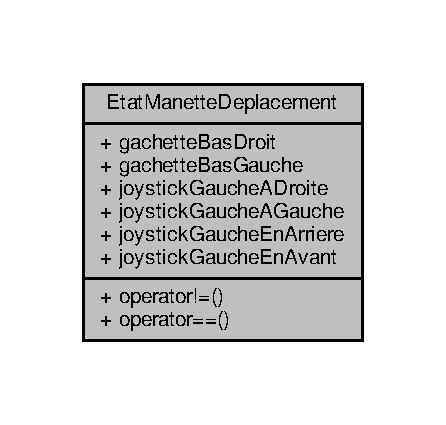
\includegraphics[width=214pt]{struct_etat_manette_deplacement__coll__graph}
\end{center}
\end{figure}
\subsubsection*{Fonctions membres publiques}
\begin{DoxyCompactItemize}
\item 
bool \hyperlink{struct_etat_manette_deplacement_aa57df0ecb60478f389d84c6e5d0cc1b8}{operator!=} (const \hyperlink{struct_etat_manette_deplacement}{Etat\+Manette\+Deplacement} \&ma\+Structure) const
\begin{DoxyCompactList}\small\item\em Surcharge de l\textquotesingle{}opérateur != afin de comparer un état de manette prédéfini avec l\textquotesingle{}état actuel de la manette. \end{DoxyCompactList}\item 
bool \hyperlink{struct_etat_manette_deplacement_a8f248b6ec1788c058e161b74fb371c5b}{operator==} (const \hyperlink{struct_etat_manette_deplacement}{Etat\+Manette\+Deplacement} \&ma\+Structure) const
\begin{DoxyCompactList}\small\item\em Surcharge de l\textquotesingle{}opérateur == afin de comparer un état de manette prédéfini avec l\textquotesingle{}état actuel de la manette. \end{DoxyCompactList}\end{DoxyCompactItemize}
\subsubsection*{Attributs publics}
\begin{DoxyCompactItemize}
\item 
bool \hyperlink{struct_etat_manette_deplacement_a4588620c1e2a3543ce67c9a791aac106}{gachette\+Bas\+Droit}
\begin{DoxyCompactList}\small\item\em Membre définissant l\textquotesingle{}état du bouton R2. \end{DoxyCompactList}\item 
bool \hyperlink{struct_etat_manette_deplacement_a0d197e25bc2e0402a068a8d012c25472}{gachette\+Bas\+Gauche}
\begin{DoxyCompactList}\small\item\em Membre définissant l\textquotesingle{}état du bouton L2. \end{DoxyCompactList}\item 
bool \hyperlink{struct_etat_manette_deplacement_a8fa93da5af430ac00ffd4ee8b76987a2}{joystick\+Gauche\+A\+Droite}
\begin{DoxyCompactList}\small\item\em Membre définissant l\textquotesingle{}état du joystick sur l\textquotesingle{}axe X. \end{DoxyCompactList}\item 
bool \hyperlink{struct_etat_manette_deplacement_af7e92a8d8f116e2bc4a5a95386f604e7}{joystick\+Gauche\+A\+Gauche}
\begin{DoxyCompactList}\small\item\em Membre définissant l\textquotesingle{}état du joystick sur l\textquotesingle{}axe X. \end{DoxyCompactList}\item 
bool \hyperlink{struct_etat_manette_deplacement_a584cf1538425c87588c5b96b79c8d482}{joystick\+Gauche\+En\+Arriere}
\begin{DoxyCompactList}\small\item\em Membre définissant l\textquotesingle{}état du joystick sur l\textquotesingle{}axe Y. \end{DoxyCompactList}\item 
bool \hyperlink{struct_etat_manette_deplacement_a8c8e3ca694408bc6a6ced4e20b9da0be}{joystick\+Gauche\+En\+Avant}
\begin{DoxyCompactList}\small\item\em Membre définissant l\textquotesingle{}état du joystick sur l\textquotesingle{}axe Y. \end{DoxyCompactList}\end{DoxyCompactItemize}


\subsubsection{Description détaillée}
Structure qui définit l\textquotesingle{}état de la manette en mode déplacement du robot. 

Définition à la ligne \hyperlink{manette_8h_source_l00178}{178} du fichier \hyperlink{manette_8h_source}{manette.\+h}.



\subsubsection{Documentation des fonctions membres}
\mbox{\Hypertarget{struct_etat_manette_deplacement_aa57df0ecb60478f389d84c6e5d0cc1b8}\label{struct_etat_manette_deplacement_aa57df0ecb60478f389d84c6e5d0cc1b8}} 
\index{Etat\+Manette\+Deplacement@{Etat\+Manette\+Deplacement}!operator"!=@{operator"!=}}
\index{operator"!=@{operator"!=}!Etat\+Manette\+Deplacement@{Etat\+Manette\+Deplacement}}
\paragraph{\texorpdfstring{operator"!=()}{operator!=()}}
{\footnotesize\ttfamily bool Etat\+Manette\+Deplacement\+::operator!= (\begin{DoxyParamCaption}\item[{const \hyperlink{struct_etat_manette_deplacement}{Etat\+Manette\+Deplacement} \&}]{ma\+Structure }\end{DoxyParamCaption}) const}



Surcharge de l\textquotesingle{}opérateur != afin de comparer un état de manette prédéfini avec l\textquotesingle{}état actuel de la manette. 


\begin{DoxyParams}{Paramètres}
{\em ma\+Structure} & \\
\hline
\end{DoxyParams}
\begin{DoxyReturn}{Renvoie}
Si l\textquotesingle{}opération est possible ou pas 
\end{DoxyReturn}


Définition à la ligne \hyperlink{manette_8cpp_source_l00654}{654} du fichier \hyperlink{manette_8cpp_source}{manette.\+cpp}.


\begin{DoxyCode}
00655 \{
00656     \textcolor{keywordflow}{return} !(*\textcolor{keyword}{this} == maStructure);
00657 \}
\end{DoxyCode}
\mbox{\Hypertarget{struct_etat_manette_deplacement_a8f248b6ec1788c058e161b74fb371c5b}\label{struct_etat_manette_deplacement_a8f248b6ec1788c058e161b74fb371c5b}} 
\index{Etat\+Manette\+Deplacement@{Etat\+Manette\+Deplacement}!operator==@{operator==}}
\index{operator==@{operator==}!Etat\+Manette\+Deplacement@{Etat\+Manette\+Deplacement}}
\paragraph{\texorpdfstring{operator==()}{operator==()}}
{\footnotesize\ttfamily bool Etat\+Manette\+Deplacement\+::operator== (\begin{DoxyParamCaption}\item[{const \hyperlink{struct_etat_manette_deplacement}{Etat\+Manette\+Deplacement} \&}]{ma\+Structure }\end{DoxyParamCaption}) const}



Surcharge de l\textquotesingle{}opérateur == afin de comparer un état de manette prédéfini avec l\textquotesingle{}état actuel de la manette. 


\begin{DoxyParams}{Paramètres}
{\em ma\+Structure} & \\
\hline
\end{DoxyParams}
\begin{DoxyReturn}{Renvoie}
Si l\textquotesingle{}opération est possible ou pas 
\end{DoxyReturn}


Définition à la ligne \hyperlink{manette_8cpp_source_l00636}{636} du fichier \hyperlink{manette_8cpp_source}{manette.\+cpp}.



Références \hyperlink{manette_8h_source_l00185}{gachette\+Bas\+Droit}, \hyperlink{manette_8h_source_l00184}{gachette\+Bas\+Gauche}, \hyperlink{manette_8h_source_l00183}{joystick\+Gauche\+A\+Droite}, \hyperlink{manette_8h_source_l00182}{joystick\+Gauche\+A\+Gauche}, \hyperlink{manette_8h_source_l00181}{joystick\+Gauche\+En\+Arriere}, et \hyperlink{manette_8h_source_l00180}{joystick\+Gauche\+En\+Avant}.


\begin{DoxyCode}
00637 \{
00638     \textcolor{keywordflow}{if}(this->\hyperlink{struct_etat_manette_deplacement_a4588620c1e2a3543ce67c9a791aac106}{gachetteBasDroit} != maStructure.\hyperlink{struct_etat_manette_deplacement_a4588620c1e2a3543ce67c9a791aac106}{gachetteBasDroit})
00639         \textcolor{keywordflow}{return} \textcolor{keyword}{false};
00640     \textcolor{keywordflow}{else} \textcolor{keywordflow}{if}(this->\hyperlink{struct_etat_manette_deplacement_a0d197e25bc2e0402a068a8d012c25472}{gachetteBasGauche} != maStructure.
      \hyperlink{struct_etat_manette_deplacement_a0d197e25bc2e0402a068a8d012c25472}{gachetteBasGauche})
00641         \textcolor{keywordflow}{return} \textcolor{keyword}{false};
00642     \textcolor{keywordflow}{else} \textcolor{keywordflow}{if}(this->\hyperlink{struct_etat_manette_deplacement_a8fa93da5af430ac00ffd4ee8b76987a2}{joystickGaucheADroite} != maStructure.
      \hyperlink{struct_etat_manette_deplacement_a8fa93da5af430ac00ffd4ee8b76987a2}{joystickGaucheADroite})
00643         \textcolor{keywordflow}{return} \textcolor{keyword}{false};
00644     \textcolor{keywordflow}{else} \textcolor{keywordflow}{if}(this->\hyperlink{struct_etat_manette_deplacement_af7e92a8d8f116e2bc4a5a95386f604e7}{joystickGaucheAGauche} != maStructure.
      \hyperlink{struct_etat_manette_deplacement_af7e92a8d8f116e2bc4a5a95386f604e7}{joystickGaucheAGauche})
00645         \textcolor{keywordflow}{return} \textcolor{keyword}{false};
00646     \textcolor{keywordflow}{else} \textcolor{keywordflow}{if}(this->\hyperlink{struct_etat_manette_deplacement_a584cf1538425c87588c5b96b79c8d482}{joystickGaucheEnArriere} != maStructure.
      \hyperlink{struct_etat_manette_deplacement_a584cf1538425c87588c5b96b79c8d482}{joystickGaucheEnArriere})
00647         \textcolor{keywordflow}{return} \textcolor{keyword}{false};
00648     \textcolor{keywordflow}{else} \textcolor{keywordflow}{if}(this->\hyperlink{struct_etat_manette_deplacement_a8c8e3ca694408bc6a6ced4e20b9da0be}{joystickGaucheEnAvant} != maStructure.
      \hyperlink{struct_etat_manette_deplacement_a8c8e3ca694408bc6a6ced4e20b9da0be}{joystickGaucheEnAvant})
00649         \textcolor{keywordflow}{return} \textcolor{keyword}{false};
00650     \textcolor{keywordflow}{else}
00651         \textcolor{keywordflow}{return} \textcolor{keyword}{true};
00652 \}
\end{DoxyCode}


\subsubsection{Documentation des données membres}
\mbox{\Hypertarget{struct_etat_manette_deplacement_a4588620c1e2a3543ce67c9a791aac106}\label{struct_etat_manette_deplacement_a4588620c1e2a3543ce67c9a791aac106}} 
\index{Etat\+Manette\+Deplacement@{Etat\+Manette\+Deplacement}!gachette\+Bas\+Droit@{gachette\+Bas\+Droit}}
\index{gachette\+Bas\+Droit@{gachette\+Bas\+Droit}!Etat\+Manette\+Deplacement@{Etat\+Manette\+Deplacement}}
\paragraph{\texorpdfstring{gachette\+Bas\+Droit}{gachetteBasDroit}}
{\footnotesize\ttfamily bool Etat\+Manette\+Deplacement\+::gachette\+Bas\+Droit}



Membre définissant l\textquotesingle{}état du bouton R2. 



Définition à la ligne \hyperlink{manette_8h_source_l00185}{185} du fichier \hyperlink{manette_8h_source}{manette.\+h}.



Référencé par \hyperlink{manette_8cpp_source_l00504}{Manette\+::changer\+Gachette\+Bas\+Droit()}, \hyperlink{manette_8cpp_source_l00178}{Manette\+::initialisation\+Structure\+Rotation\+A\+Droite()}, \hyperlink{manette_8cpp_source_l00151}{Manette\+::initialisation\+Structure\+Rotation\+A\+Gauche()}, \hyperlink{manette_8cpp_source_l00127}{Manette\+::initialisation\+Structures\+En\+Arriere()}, \hyperlink{manette_8cpp_source_l00103}{Manette\+::initialisation\+Structures\+En\+Avant()}, \hyperlink{manette_8cpp_source_l00188}{Manette\+::initialisation\+Structures\+Rotation\+A\+Droite\+Doucement()}, \hyperlink{manette_8cpp_source_l00161}{Manette\+::initialisation\+Structures\+Rotation\+A\+Gauche\+Doucement()}, \hyperlink{manette_8cpp_source_l00296}{Manette\+::initialisation\+Structures\+Virage\+Arriere\+A\+Droite\+Doucement()}, \hyperlink{manette_8cpp_source_l00269}{Manette\+::initialisation\+Structures\+Virage\+Arriere\+A\+Gauche\+Doucement()}, \hyperlink{manette_8cpp_source_l00242}{Manette\+::initialisation\+Structures\+Virage\+Avant\+A\+Droite\+Doucement()}, \hyperlink{manette_8cpp_source_l00215}{Manette\+::initialisation\+Structures\+Virage\+Avant\+A\+Gauche\+Doucement()}, \hyperlink{manette_8cpp_source_l00286}{Manette\+::initialisation\+Structure\+Virage\+Arriere\+A\+Droite()}, \hyperlink{manette_8cpp_source_l00259}{Manette\+::initialisation\+Structure\+Virage\+Arriere\+A\+Gauche()}, \hyperlink{manette_8cpp_source_l00232}{Manette\+::initialisation\+Structure\+Virage\+Avant\+A\+Droite()}, \hyperlink{manette_8cpp_source_l00205}{Manette\+::initialisation\+Structure\+Virage\+Avant\+A\+Gauche()}, \hyperlink{manette_8cpp_source_l00023}{Manette\+::initialiser\+Etats()}, et \hyperlink{manette_8cpp_source_l00636}{operator==()}.

\mbox{\Hypertarget{struct_etat_manette_deplacement_a0d197e25bc2e0402a068a8d012c25472}\label{struct_etat_manette_deplacement_a0d197e25bc2e0402a068a8d012c25472}} 
\index{Etat\+Manette\+Deplacement@{Etat\+Manette\+Deplacement}!gachette\+Bas\+Gauche@{gachette\+Bas\+Gauche}}
\index{gachette\+Bas\+Gauche@{gachette\+Bas\+Gauche}!Etat\+Manette\+Deplacement@{Etat\+Manette\+Deplacement}}
\paragraph{\texorpdfstring{gachette\+Bas\+Gauche}{gachetteBasGauche}}
{\footnotesize\ttfamily bool Etat\+Manette\+Deplacement\+::gachette\+Bas\+Gauche}



Membre définissant l\textquotesingle{}état du bouton L2. 



Définition à la ligne \hyperlink{manette_8h_source_l00184}{184} du fichier \hyperlink{manette_8h_source}{manette.\+h}.



Référencé par \hyperlink{manette_8cpp_source_l00493}{Manette\+::changer\+Gachette\+Bas\+Gauche()}, \hyperlink{manette_8cpp_source_l00178}{Manette\+::initialisation\+Structure\+Rotation\+A\+Droite()}, \hyperlink{manette_8cpp_source_l00151}{Manette\+::initialisation\+Structure\+Rotation\+A\+Gauche()}, \hyperlink{manette_8cpp_source_l00127}{Manette\+::initialisation\+Structures\+En\+Arriere()}, \hyperlink{manette_8cpp_source_l00103}{Manette\+::initialisation\+Structures\+En\+Avant()}, \hyperlink{manette_8cpp_source_l00188}{Manette\+::initialisation\+Structures\+Rotation\+A\+Droite\+Doucement()}, \hyperlink{manette_8cpp_source_l00161}{Manette\+::initialisation\+Structures\+Rotation\+A\+Gauche\+Doucement()}, \hyperlink{manette_8cpp_source_l00296}{Manette\+::initialisation\+Structures\+Virage\+Arriere\+A\+Droite\+Doucement()}, \hyperlink{manette_8cpp_source_l00269}{Manette\+::initialisation\+Structures\+Virage\+Arriere\+A\+Gauche\+Doucement()}, \hyperlink{manette_8cpp_source_l00242}{Manette\+::initialisation\+Structures\+Virage\+Avant\+A\+Droite\+Doucement()}, \hyperlink{manette_8cpp_source_l00215}{Manette\+::initialisation\+Structures\+Virage\+Avant\+A\+Gauche\+Doucement()}, \hyperlink{manette_8cpp_source_l00286}{Manette\+::initialisation\+Structure\+Virage\+Arriere\+A\+Droite()}, \hyperlink{manette_8cpp_source_l00259}{Manette\+::initialisation\+Structure\+Virage\+Arriere\+A\+Gauche()}, \hyperlink{manette_8cpp_source_l00232}{Manette\+::initialisation\+Structure\+Virage\+Avant\+A\+Droite()}, \hyperlink{manette_8cpp_source_l00205}{Manette\+::initialisation\+Structure\+Virage\+Avant\+A\+Gauche()}, \hyperlink{manette_8cpp_source_l00023}{Manette\+::initialiser\+Etats()}, et \hyperlink{manette_8cpp_source_l00636}{operator==()}.

\mbox{\Hypertarget{struct_etat_manette_deplacement_a8fa93da5af430ac00ffd4ee8b76987a2}\label{struct_etat_manette_deplacement_a8fa93da5af430ac00ffd4ee8b76987a2}} 
\index{Etat\+Manette\+Deplacement@{Etat\+Manette\+Deplacement}!joystick\+Gauche\+A\+Droite@{joystick\+Gauche\+A\+Droite}}
\index{joystick\+Gauche\+A\+Droite@{joystick\+Gauche\+A\+Droite}!Etat\+Manette\+Deplacement@{Etat\+Manette\+Deplacement}}
\paragraph{\texorpdfstring{joystick\+Gauche\+A\+Droite}{joystickGaucheADroite}}
{\footnotesize\ttfamily bool Etat\+Manette\+Deplacement\+::joystick\+Gauche\+A\+Droite}



Membre définissant l\textquotesingle{}état du joystick sur l\textquotesingle{}axe X. 



Définition à la ligne \hyperlink{manette_8h_source_l00183}{183} du fichier \hyperlink{manette_8h_source}{manette.\+h}.



Référencé par \hyperlink{manette_8cpp_source_l00421}{Manette\+::changer\+Axe\+X\+Joystick\+Gauche()}, \hyperlink{manette_8cpp_source_l00178}{Manette\+::initialisation\+Structure\+Rotation\+A\+Droite()}, \hyperlink{manette_8cpp_source_l00151}{Manette\+::initialisation\+Structure\+Rotation\+A\+Gauche()}, \hyperlink{manette_8cpp_source_l00127}{Manette\+::initialisation\+Structures\+En\+Arriere()}, \hyperlink{manette_8cpp_source_l00103}{Manette\+::initialisation\+Structures\+En\+Avant()}, \hyperlink{manette_8cpp_source_l00188}{Manette\+::initialisation\+Structures\+Rotation\+A\+Droite\+Doucement()}, \hyperlink{manette_8cpp_source_l00161}{Manette\+::initialisation\+Structures\+Rotation\+A\+Gauche\+Doucement()}, \hyperlink{manette_8cpp_source_l00296}{Manette\+::initialisation\+Structures\+Virage\+Arriere\+A\+Droite\+Doucement()}, \hyperlink{manette_8cpp_source_l00269}{Manette\+::initialisation\+Structures\+Virage\+Arriere\+A\+Gauche\+Doucement()}, \hyperlink{manette_8cpp_source_l00242}{Manette\+::initialisation\+Structures\+Virage\+Avant\+A\+Droite\+Doucement()}, \hyperlink{manette_8cpp_source_l00215}{Manette\+::initialisation\+Structures\+Virage\+Avant\+A\+Gauche\+Doucement()}, \hyperlink{manette_8cpp_source_l00286}{Manette\+::initialisation\+Structure\+Virage\+Arriere\+A\+Droite()}, \hyperlink{manette_8cpp_source_l00259}{Manette\+::initialisation\+Structure\+Virage\+Arriere\+A\+Gauche()}, \hyperlink{manette_8cpp_source_l00232}{Manette\+::initialisation\+Structure\+Virage\+Avant\+A\+Droite()}, \hyperlink{manette_8cpp_source_l00205}{Manette\+::initialisation\+Structure\+Virage\+Avant\+A\+Gauche()}, \hyperlink{manette_8cpp_source_l00023}{Manette\+::initialiser\+Etats()}, et \hyperlink{manette_8cpp_source_l00636}{operator==()}.

\mbox{\Hypertarget{struct_etat_manette_deplacement_af7e92a8d8f116e2bc4a5a95386f604e7}\label{struct_etat_manette_deplacement_af7e92a8d8f116e2bc4a5a95386f604e7}} 
\index{Etat\+Manette\+Deplacement@{Etat\+Manette\+Deplacement}!joystick\+Gauche\+A\+Gauche@{joystick\+Gauche\+A\+Gauche}}
\index{joystick\+Gauche\+A\+Gauche@{joystick\+Gauche\+A\+Gauche}!Etat\+Manette\+Deplacement@{Etat\+Manette\+Deplacement}}
\paragraph{\texorpdfstring{joystick\+Gauche\+A\+Gauche}{joystickGaucheAGauche}}
{\footnotesize\ttfamily bool Etat\+Manette\+Deplacement\+::joystick\+Gauche\+A\+Gauche}



Membre définissant l\textquotesingle{}état du joystick sur l\textquotesingle{}axe X. 



Définition à la ligne \hyperlink{manette_8h_source_l00182}{182} du fichier \hyperlink{manette_8h_source}{manette.\+h}.



Référencé par \hyperlink{manette_8cpp_source_l00421}{Manette\+::changer\+Axe\+X\+Joystick\+Gauche()}, \hyperlink{manette_8cpp_source_l00178}{Manette\+::initialisation\+Structure\+Rotation\+A\+Droite()}, \hyperlink{manette_8cpp_source_l00151}{Manette\+::initialisation\+Structure\+Rotation\+A\+Gauche()}, \hyperlink{manette_8cpp_source_l00127}{Manette\+::initialisation\+Structures\+En\+Arriere()}, \hyperlink{manette_8cpp_source_l00103}{Manette\+::initialisation\+Structures\+En\+Avant()}, \hyperlink{manette_8cpp_source_l00188}{Manette\+::initialisation\+Structures\+Rotation\+A\+Droite\+Doucement()}, \hyperlink{manette_8cpp_source_l00161}{Manette\+::initialisation\+Structures\+Rotation\+A\+Gauche\+Doucement()}, \hyperlink{manette_8cpp_source_l00296}{Manette\+::initialisation\+Structures\+Virage\+Arriere\+A\+Droite\+Doucement()}, \hyperlink{manette_8cpp_source_l00269}{Manette\+::initialisation\+Structures\+Virage\+Arriere\+A\+Gauche\+Doucement()}, \hyperlink{manette_8cpp_source_l00242}{Manette\+::initialisation\+Structures\+Virage\+Avant\+A\+Droite\+Doucement()}, \hyperlink{manette_8cpp_source_l00215}{Manette\+::initialisation\+Structures\+Virage\+Avant\+A\+Gauche\+Doucement()}, \hyperlink{manette_8cpp_source_l00286}{Manette\+::initialisation\+Structure\+Virage\+Arriere\+A\+Droite()}, \hyperlink{manette_8cpp_source_l00259}{Manette\+::initialisation\+Structure\+Virage\+Arriere\+A\+Gauche()}, \hyperlink{manette_8cpp_source_l00232}{Manette\+::initialisation\+Structure\+Virage\+Avant\+A\+Droite()}, \hyperlink{manette_8cpp_source_l00205}{Manette\+::initialisation\+Structure\+Virage\+Avant\+A\+Gauche()}, \hyperlink{manette_8cpp_source_l00023}{Manette\+::initialiser\+Etats()}, et \hyperlink{manette_8cpp_source_l00636}{operator==()}.

\mbox{\Hypertarget{struct_etat_manette_deplacement_a584cf1538425c87588c5b96b79c8d482}\label{struct_etat_manette_deplacement_a584cf1538425c87588c5b96b79c8d482}} 
\index{Etat\+Manette\+Deplacement@{Etat\+Manette\+Deplacement}!joystick\+Gauche\+En\+Arriere@{joystick\+Gauche\+En\+Arriere}}
\index{joystick\+Gauche\+En\+Arriere@{joystick\+Gauche\+En\+Arriere}!Etat\+Manette\+Deplacement@{Etat\+Manette\+Deplacement}}
\paragraph{\texorpdfstring{joystick\+Gauche\+En\+Arriere}{joystickGaucheEnArriere}}
{\footnotesize\ttfamily bool Etat\+Manette\+Deplacement\+::joystick\+Gauche\+En\+Arriere}



Membre définissant l\textquotesingle{}état du joystick sur l\textquotesingle{}axe Y. 



Définition à la ligne \hyperlink{manette_8h_source_l00181}{181} du fichier \hyperlink{manette_8h_source}{manette.\+h}.



Référencé par \hyperlink{manette_8cpp_source_l00438}{Manette\+::changer\+Axe\+Y\+Joystick\+Gauche()}, \hyperlink{manette_8cpp_source_l00178}{Manette\+::initialisation\+Structure\+Rotation\+A\+Droite()}, \hyperlink{manette_8cpp_source_l00151}{Manette\+::initialisation\+Structure\+Rotation\+A\+Gauche()}, \hyperlink{manette_8cpp_source_l00127}{Manette\+::initialisation\+Structures\+En\+Arriere()}, \hyperlink{manette_8cpp_source_l00103}{Manette\+::initialisation\+Structures\+En\+Avant()}, \hyperlink{manette_8cpp_source_l00188}{Manette\+::initialisation\+Structures\+Rotation\+A\+Droite\+Doucement()}, \hyperlink{manette_8cpp_source_l00161}{Manette\+::initialisation\+Structures\+Rotation\+A\+Gauche\+Doucement()}, \hyperlink{manette_8cpp_source_l00296}{Manette\+::initialisation\+Structures\+Virage\+Arriere\+A\+Droite\+Doucement()}, \hyperlink{manette_8cpp_source_l00269}{Manette\+::initialisation\+Structures\+Virage\+Arriere\+A\+Gauche\+Doucement()}, \hyperlink{manette_8cpp_source_l00242}{Manette\+::initialisation\+Structures\+Virage\+Avant\+A\+Droite\+Doucement()}, \hyperlink{manette_8cpp_source_l00215}{Manette\+::initialisation\+Structures\+Virage\+Avant\+A\+Gauche\+Doucement()}, \hyperlink{manette_8cpp_source_l00286}{Manette\+::initialisation\+Structure\+Virage\+Arriere\+A\+Droite()}, \hyperlink{manette_8cpp_source_l00259}{Manette\+::initialisation\+Structure\+Virage\+Arriere\+A\+Gauche()}, \hyperlink{manette_8cpp_source_l00232}{Manette\+::initialisation\+Structure\+Virage\+Avant\+A\+Droite()}, \hyperlink{manette_8cpp_source_l00205}{Manette\+::initialisation\+Structure\+Virage\+Avant\+A\+Gauche()}, \hyperlink{manette_8cpp_source_l00023}{Manette\+::initialiser\+Etats()}, et \hyperlink{manette_8cpp_source_l00636}{operator==()}.

\mbox{\Hypertarget{struct_etat_manette_deplacement_a8c8e3ca694408bc6a6ced4e20b9da0be}\label{struct_etat_manette_deplacement_a8c8e3ca694408bc6a6ced4e20b9da0be}} 
\index{Etat\+Manette\+Deplacement@{Etat\+Manette\+Deplacement}!joystick\+Gauche\+En\+Avant@{joystick\+Gauche\+En\+Avant}}
\index{joystick\+Gauche\+En\+Avant@{joystick\+Gauche\+En\+Avant}!Etat\+Manette\+Deplacement@{Etat\+Manette\+Deplacement}}
\paragraph{\texorpdfstring{joystick\+Gauche\+En\+Avant}{joystickGaucheEnAvant}}
{\footnotesize\ttfamily bool Etat\+Manette\+Deplacement\+::joystick\+Gauche\+En\+Avant}



Membre définissant l\textquotesingle{}état du joystick sur l\textquotesingle{}axe Y. 



Définition à la ligne \hyperlink{manette_8h_source_l00180}{180} du fichier \hyperlink{manette_8h_source}{manette.\+h}.



Référencé par \hyperlink{manette_8cpp_source_l00438}{Manette\+::changer\+Axe\+Y\+Joystick\+Gauche()}, \hyperlink{manette_8cpp_source_l00178}{Manette\+::initialisation\+Structure\+Rotation\+A\+Droite()}, \hyperlink{manette_8cpp_source_l00151}{Manette\+::initialisation\+Structure\+Rotation\+A\+Gauche()}, \hyperlink{manette_8cpp_source_l00127}{Manette\+::initialisation\+Structures\+En\+Arriere()}, \hyperlink{manette_8cpp_source_l00103}{Manette\+::initialisation\+Structures\+En\+Avant()}, \hyperlink{manette_8cpp_source_l00188}{Manette\+::initialisation\+Structures\+Rotation\+A\+Droite\+Doucement()}, \hyperlink{manette_8cpp_source_l00161}{Manette\+::initialisation\+Structures\+Rotation\+A\+Gauche\+Doucement()}, \hyperlink{manette_8cpp_source_l00296}{Manette\+::initialisation\+Structures\+Virage\+Arriere\+A\+Droite\+Doucement()}, \hyperlink{manette_8cpp_source_l00269}{Manette\+::initialisation\+Structures\+Virage\+Arriere\+A\+Gauche\+Doucement()}, \hyperlink{manette_8cpp_source_l00242}{Manette\+::initialisation\+Structures\+Virage\+Avant\+A\+Droite\+Doucement()}, \hyperlink{manette_8cpp_source_l00215}{Manette\+::initialisation\+Structures\+Virage\+Avant\+A\+Gauche\+Doucement()}, \hyperlink{manette_8cpp_source_l00286}{Manette\+::initialisation\+Structure\+Virage\+Arriere\+A\+Droite()}, \hyperlink{manette_8cpp_source_l00259}{Manette\+::initialisation\+Structure\+Virage\+Arriere\+A\+Gauche()}, \hyperlink{manette_8cpp_source_l00232}{Manette\+::initialisation\+Structure\+Virage\+Avant\+A\+Droite()}, \hyperlink{manette_8cpp_source_l00205}{Manette\+::initialisation\+Structure\+Virage\+Avant\+A\+Gauche()}, \hyperlink{manette_8cpp_source_l00023}{Manette\+::initialiser\+Etats()}, et \hyperlink{manette_8cpp_source_l00636}{operator==()}.



La documentation de cette structure a été générée à partir des fichiers suivants \+:\begin{DoxyCompactItemize}
\item 
\hyperlink{manette_8h}{manette.\+h}\item 
\hyperlink{manette_8cpp}{manette.\+cpp}\end{DoxyCompactItemize}

\hypertarget{struct_etat_manette_pilotage}{}\subsection{Référence de la structure Etat\+Manette\+Pilotage}
\label{struct_etat_manette_pilotage}\index{Etat\+Manette\+Pilotage@{Etat\+Manette\+Pilotage}}


Structure qui définit l\textquotesingle{}état de la manette en mode pilotage de la pince.  




{\ttfamily \#include $<$manette.\+h$>$}



Graphe de collaboration de Etat\+Manette\+Pilotage\+:\nopagebreak
\begin{figure}[H]
\begin{center}
\leavevmode
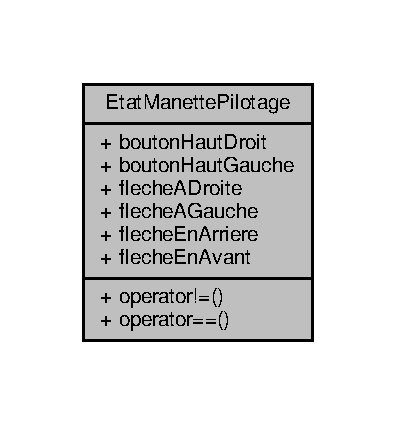
\includegraphics[width=190pt]{struct_etat_manette_pilotage__coll__graph}
\end{center}
\end{figure}
\subsubsection*{Fonctions membres publiques}
\begin{DoxyCompactItemize}
\item 
bool \hyperlink{struct_etat_manette_pilotage_a1a9cbf7891c30ab2503ec9c9b7fb5299}{operator!=} (const \hyperlink{struct_etat_manette_pilotage}{Etat\+Manette\+Pilotage} \&ma\+Structure) const
\begin{DoxyCompactList}\small\item\em Surcharge de l\textquotesingle{}opérateur != afin de comparer un état de manette prédéfini avec l\textquotesingle{}état actuel de la manette. \end{DoxyCompactList}\item 
bool \hyperlink{struct_etat_manette_pilotage_a85cac8d658fdc2d63ac54ea340ec8be8}{operator==} (const \hyperlink{struct_etat_manette_pilotage}{Etat\+Manette\+Pilotage} \&ma\+Structure) const
\begin{DoxyCompactList}\small\item\em Surcharge de l\textquotesingle{}opérateur == afin de comparer un état de manette prédéfini avec l\textquotesingle{}état actuel de la manette. \end{DoxyCompactList}\end{DoxyCompactItemize}
\subsubsection*{Attributs publics}
\begin{DoxyCompactItemize}
\item 
bool \hyperlink{struct_etat_manette_pilotage_ae0ca75dab8c31fe26d440ec319e2fa84}{bouton\+Haut\+Droit}
\begin{DoxyCompactList}\small\item\em Membre définissant l\textquotesingle{}état du bouton R1. \end{DoxyCompactList}\item 
bool \hyperlink{struct_etat_manette_pilotage_aef8579e406e8766c1936db6da460492a}{bouton\+Haut\+Gauche}
\begin{DoxyCompactList}\small\item\em Membre définissant l\textquotesingle{}état du bouton L1. \end{DoxyCompactList}\item 
bool \hyperlink{struct_etat_manette_pilotage_a78a791f6f8968042efd8e2f64f70f882}{fleche\+A\+Droite}
\begin{DoxyCompactList}\small\item\em Membre définissant l\textquotesingle{}état de la flèche de droite. \end{DoxyCompactList}\item 
bool \hyperlink{struct_etat_manette_pilotage_aace02b9bb3feb3b618dd9133d4c5b87f}{fleche\+A\+Gauche}
\begin{DoxyCompactList}\small\item\em Membre définissant l\textquotesingle{}état de la flèche de gauche. \end{DoxyCompactList}\item 
bool \hyperlink{struct_etat_manette_pilotage_ab7cce4480358d2e7ac189e96ab04b894}{fleche\+En\+Arriere}
\begin{DoxyCompactList}\small\item\em Membre définissant l\textquotesingle{}état de la flèche du bas. \end{DoxyCompactList}\item 
bool \hyperlink{struct_etat_manette_pilotage_a12429b457b51cb45cc9d405f3a01bea6}{fleche\+En\+Avant}
\begin{DoxyCompactList}\small\item\em Membre définissant l\textquotesingle{}état de la flèche du haut. \end{DoxyCompactList}\end{DoxyCompactItemize}


\subsubsection{Description détaillée}
Structure qui définit l\textquotesingle{}état de la manette en mode pilotage de la pince. 

Définition à la ligne \hyperlink{manette_8h_source_l00150}{150} du fichier \hyperlink{manette_8h_source}{manette.\+h}.



\subsubsection{Documentation des fonctions membres}
\mbox{\Hypertarget{struct_etat_manette_pilotage_a1a9cbf7891c30ab2503ec9c9b7fb5299}\label{struct_etat_manette_pilotage_a1a9cbf7891c30ab2503ec9c9b7fb5299}} 
\index{Etat\+Manette\+Pilotage@{Etat\+Manette\+Pilotage}!operator"!=@{operator"!=}}
\index{operator"!=@{operator"!=}!Etat\+Manette\+Pilotage@{Etat\+Manette\+Pilotage}}
\paragraph{\texorpdfstring{operator"!=()}{operator!=()}}
{\footnotesize\ttfamily bool Etat\+Manette\+Pilotage\+::operator!= (\begin{DoxyParamCaption}\item[{const \hyperlink{struct_etat_manette_pilotage}{Etat\+Manette\+Pilotage} \&}]{ma\+Structure }\end{DoxyParamCaption}) const}



Surcharge de l\textquotesingle{}opérateur != afin de comparer un état de manette prédéfini avec l\textquotesingle{}état actuel de la manette. 


\begin{DoxyParams}{Paramètres}
{\em ma\+Structure} & \\
\hline
\end{DoxyParams}
\begin{DoxyReturn}{Renvoie}
Si l\textquotesingle{}opération est possible ou pas 
\end{DoxyReturn}


Définition à la ligne \hyperlink{manette_8cpp_source_l00631}{631} du fichier \hyperlink{manette_8cpp_source}{manette.\+cpp}.


\begin{DoxyCode}
00632 \{
00633     \textcolor{keywordflow}{return} !(*\textcolor{keyword}{this} == maStructure);
00634 \}
\end{DoxyCode}
\mbox{\Hypertarget{struct_etat_manette_pilotage_a85cac8d658fdc2d63ac54ea340ec8be8}\label{struct_etat_manette_pilotage_a85cac8d658fdc2d63ac54ea340ec8be8}} 
\index{Etat\+Manette\+Pilotage@{Etat\+Manette\+Pilotage}!operator==@{operator==}}
\index{operator==@{operator==}!Etat\+Manette\+Pilotage@{Etat\+Manette\+Pilotage}}
\paragraph{\texorpdfstring{operator==()}{operator==()}}
{\footnotesize\ttfamily bool Etat\+Manette\+Pilotage\+::operator== (\begin{DoxyParamCaption}\item[{const \hyperlink{struct_etat_manette_pilotage}{Etat\+Manette\+Pilotage} \&}]{ma\+Structure }\end{DoxyParamCaption}) const}



Surcharge de l\textquotesingle{}opérateur == afin de comparer un état de manette prédéfini avec l\textquotesingle{}état actuel de la manette. 


\begin{DoxyParams}{Paramètres}
{\em ma\+Structure} & \\
\hline
\end{DoxyParams}
\begin{DoxyReturn}{Renvoie}
Si l\textquotesingle{}opération est possible ou pas 
\end{DoxyReturn}


Définition à la ligne \hyperlink{manette_8cpp_source_l00613}{613} du fichier \hyperlink{manette_8cpp_source}{manette.\+cpp}.



Références \hyperlink{manette_8h_source_l00157}{bouton\+Haut\+Droit}, \hyperlink{manette_8h_source_l00156}{bouton\+Haut\+Gauche}, \hyperlink{manette_8h_source_l00155}{fleche\+A\+Droite}, \hyperlink{manette_8h_source_l00154}{fleche\+A\+Gauche}, \hyperlink{manette_8h_source_l00153}{fleche\+En\+Arriere}, et \hyperlink{manette_8h_source_l00152}{fleche\+En\+Avant}.


\begin{DoxyCode}
00614 \{
00615     \textcolor{keywordflow}{if}(this->\hyperlink{struct_etat_manette_pilotage_a12429b457b51cb45cc9d405f3a01bea6}{flecheEnAvant} != maStructure.\hyperlink{struct_etat_manette_pilotage_a12429b457b51cb45cc9d405f3a01bea6}{flecheEnAvant})
00616         \textcolor{keywordflow}{return} \textcolor{keyword}{false};
00617     \textcolor{keywordflow}{else} \textcolor{keywordflow}{if}(this->\hyperlink{struct_etat_manette_pilotage_ab7cce4480358d2e7ac189e96ab04b894}{flecheEnArriere} != maStructure.\hyperlink{struct_etat_manette_pilotage_ab7cce4480358d2e7ac189e96ab04b894}{flecheEnArriere})
00618         \textcolor{keywordflow}{return} \textcolor{keyword}{false};
00619     \textcolor{keywordflow}{else} \textcolor{keywordflow}{if}(this->\hyperlink{struct_etat_manette_pilotage_aace02b9bb3feb3b618dd9133d4c5b87f}{flecheAGauche} != maStructure.\hyperlink{struct_etat_manette_pilotage_aace02b9bb3feb3b618dd9133d4c5b87f}{flecheAGauche})
00620         \textcolor{keywordflow}{return} \textcolor{keyword}{false};
00621     \textcolor{keywordflow}{else} \textcolor{keywordflow}{if}(this->\hyperlink{struct_etat_manette_pilotage_a78a791f6f8968042efd8e2f64f70f882}{flecheADroite} != maStructure.\hyperlink{struct_etat_manette_pilotage_a78a791f6f8968042efd8e2f64f70f882}{flecheADroite})
00622         \textcolor{keywordflow}{return} \textcolor{keyword}{false};
00623     \textcolor{keywordflow}{else} \textcolor{keywordflow}{if}(this->\hyperlink{struct_etat_manette_pilotage_aef8579e406e8766c1936db6da460492a}{boutonHautGauche} != maStructure.
      \hyperlink{struct_etat_manette_pilotage_aef8579e406e8766c1936db6da460492a}{boutonHautGauche})
00624         \textcolor{keywordflow}{return} \textcolor{keyword}{false};
00625     \textcolor{keywordflow}{else} \textcolor{keywordflow}{if}(this->\hyperlink{struct_etat_manette_pilotage_ae0ca75dab8c31fe26d440ec319e2fa84}{boutonHautDroit} != maStructure.\hyperlink{struct_etat_manette_pilotage_ae0ca75dab8c31fe26d440ec319e2fa84}{boutonHautDroit})
00626         \textcolor{keywordflow}{return} \textcolor{keyword}{false};
00627     \textcolor{keywordflow}{else}
00628         \textcolor{keywordflow}{return} \textcolor{keyword}{true};
00629 \}
\end{DoxyCode}


\subsubsection{Documentation des données membres}
\mbox{\Hypertarget{struct_etat_manette_pilotage_ae0ca75dab8c31fe26d440ec319e2fa84}\label{struct_etat_manette_pilotage_ae0ca75dab8c31fe26d440ec319e2fa84}} 
\index{Etat\+Manette\+Pilotage@{Etat\+Manette\+Pilotage}!bouton\+Haut\+Droit@{bouton\+Haut\+Droit}}
\index{bouton\+Haut\+Droit@{bouton\+Haut\+Droit}!Etat\+Manette\+Pilotage@{Etat\+Manette\+Pilotage}}
\paragraph{\texorpdfstring{bouton\+Haut\+Droit}{boutonHautDroit}}
{\footnotesize\ttfamily bool Etat\+Manette\+Pilotage\+::bouton\+Haut\+Droit}



Membre définissant l\textquotesingle{}état du bouton R1. 



Définition à la ligne \hyperlink{manette_8h_source_l00157}{157} du fichier \hyperlink{manette_8h_source}{manette.\+h}.



Référencé par \hyperlink{manette_8cpp_source_l00486}{Manette\+::changer\+Bouton\+Haut\+Droit()}, \hyperlink{manette_8cpp_source_l00023}{Manette\+::initialiser\+Etats()}, \hyperlink{manette_8cpp_source_l00040}{Manette\+::initialiser\+Types\+Pilotage()}, et \hyperlink{manette_8cpp_source_l00613}{operator==()}.

\mbox{\Hypertarget{struct_etat_manette_pilotage_aef8579e406e8766c1936db6da460492a}\label{struct_etat_manette_pilotage_aef8579e406e8766c1936db6da460492a}} 
\index{Etat\+Manette\+Pilotage@{Etat\+Manette\+Pilotage}!bouton\+Haut\+Gauche@{bouton\+Haut\+Gauche}}
\index{bouton\+Haut\+Gauche@{bouton\+Haut\+Gauche}!Etat\+Manette\+Pilotage@{Etat\+Manette\+Pilotage}}
\paragraph{\texorpdfstring{bouton\+Haut\+Gauche}{boutonHautGauche}}
{\footnotesize\ttfamily bool Etat\+Manette\+Pilotage\+::bouton\+Haut\+Gauche}



Membre définissant l\textquotesingle{}état du bouton L1. 



Définition à la ligne \hyperlink{manette_8h_source_l00156}{156} du fichier \hyperlink{manette_8h_source}{manette.\+h}.



Référencé par \hyperlink{manette_8cpp_source_l00479}{Manette\+::changer\+Bouton\+Haut\+Gauche()}, \hyperlink{manette_8cpp_source_l00023}{Manette\+::initialiser\+Etats()}, \hyperlink{manette_8cpp_source_l00040}{Manette\+::initialiser\+Types\+Pilotage()}, et \hyperlink{manette_8cpp_source_l00613}{operator==()}.

\mbox{\Hypertarget{struct_etat_manette_pilotage_a78a791f6f8968042efd8e2f64f70f882}\label{struct_etat_manette_pilotage_a78a791f6f8968042efd8e2f64f70f882}} 
\index{Etat\+Manette\+Pilotage@{Etat\+Manette\+Pilotage}!fleche\+A\+Droite@{fleche\+A\+Droite}}
\index{fleche\+A\+Droite@{fleche\+A\+Droite}!Etat\+Manette\+Pilotage@{Etat\+Manette\+Pilotage}}
\paragraph{\texorpdfstring{fleche\+A\+Droite}{flecheADroite}}
{\footnotesize\ttfamily bool Etat\+Manette\+Pilotage\+::fleche\+A\+Droite}



Membre définissant l\textquotesingle{}état de la flèche de droite. 



Définition à la ligne \hyperlink{manette_8h_source_l00155}{155} du fichier \hyperlink{manette_8h_source}{manette.\+h}.



Référencé par \hyperlink{manette_8cpp_source_l00542}{Manette\+::changer\+Fleche\+A\+Droite()}, \hyperlink{manette_8cpp_source_l00023}{Manette\+::initialiser\+Etats()}, \hyperlink{manette_8cpp_source_l00040}{Manette\+::initialiser\+Types\+Pilotage()}, et \hyperlink{manette_8cpp_source_l00613}{operator==()}.

\mbox{\Hypertarget{struct_etat_manette_pilotage_aace02b9bb3feb3b618dd9133d4c5b87f}\label{struct_etat_manette_pilotage_aace02b9bb3feb3b618dd9133d4c5b87f}} 
\index{Etat\+Manette\+Pilotage@{Etat\+Manette\+Pilotage}!fleche\+A\+Gauche@{fleche\+A\+Gauche}}
\index{fleche\+A\+Gauche@{fleche\+A\+Gauche}!Etat\+Manette\+Pilotage@{Etat\+Manette\+Pilotage}}
\paragraph{\texorpdfstring{fleche\+A\+Gauche}{flecheAGauche}}
{\footnotesize\ttfamily bool Etat\+Manette\+Pilotage\+::fleche\+A\+Gauche}



Membre définissant l\textquotesingle{}état de la flèche de gauche. 



Définition à la ligne \hyperlink{manette_8h_source_l00154}{154} du fichier \hyperlink{manette_8h_source}{manette.\+h}.



Référencé par \hyperlink{manette_8cpp_source_l00533}{Manette\+::changer\+Fleche\+A\+Gauche()}, \hyperlink{manette_8cpp_source_l00023}{Manette\+::initialiser\+Etats()}, \hyperlink{manette_8cpp_source_l00040}{Manette\+::initialiser\+Types\+Pilotage()}, et \hyperlink{manette_8cpp_source_l00613}{operator==()}.

\mbox{\Hypertarget{struct_etat_manette_pilotage_ab7cce4480358d2e7ac189e96ab04b894}\label{struct_etat_manette_pilotage_ab7cce4480358d2e7ac189e96ab04b894}} 
\index{Etat\+Manette\+Pilotage@{Etat\+Manette\+Pilotage}!fleche\+En\+Arriere@{fleche\+En\+Arriere}}
\index{fleche\+En\+Arriere@{fleche\+En\+Arriere}!Etat\+Manette\+Pilotage@{Etat\+Manette\+Pilotage}}
\paragraph{\texorpdfstring{fleche\+En\+Arriere}{flecheEnArriere}}
{\footnotesize\ttfamily bool Etat\+Manette\+Pilotage\+::fleche\+En\+Arriere}



Membre définissant l\textquotesingle{}état de la flèche du bas. 



Définition à la ligne \hyperlink{manette_8h_source_l00153}{153} du fichier \hyperlink{manette_8h_source}{manette.\+h}.



Référencé par \hyperlink{manette_8cpp_source_l00524}{Manette\+::changer\+Fleche\+En\+Arriere()}, \hyperlink{manette_8cpp_source_l00023}{Manette\+::initialiser\+Etats()}, \hyperlink{manette_8cpp_source_l00040}{Manette\+::initialiser\+Types\+Pilotage()}, et \hyperlink{manette_8cpp_source_l00613}{operator==()}.

\mbox{\Hypertarget{struct_etat_manette_pilotage_a12429b457b51cb45cc9d405f3a01bea6}\label{struct_etat_manette_pilotage_a12429b457b51cb45cc9d405f3a01bea6}} 
\index{Etat\+Manette\+Pilotage@{Etat\+Manette\+Pilotage}!fleche\+En\+Avant@{fleche\+En\+Avant}}
\index{fleche\+En\+Avant@{fleche\+En\+Avant}!Etat\+Manette\+Pilotage@{Etat\+Manette\+Pilotage}}
\paragraph{\texorpdfstring{fleche\+En\+Avant}{flecheEnAvant}}
{\footnotesize\ttfamily bool Etat\+Manette\+Pilotage\+::fleche\+En\+Avant}



Membre définissant l\textquotesingle{}état de la flèche du haut. 



Définition à la ligne \hyperlink{manette_8h_source_l00152}{152} du fichier \hyperlink{manette_8h_source}{manette.\+h}.



Référencé par \hyperlink{manette_8cpp_source_l00515}{Manette\+::changer\+Fleche\+En\+Avant()}, \hyperlink{manette_8cpp_source_l00023}{Manette\+::initialiser\+Etats()}, \hyperlink{manette_8cpp_source_l00040}{Manette\+::initialiser\+Types\+Pilotage()}, et \hyperlink{manette_8cpp_source_l00613}{operator==()}.



La documentation de cette structure a été générée à partir des fichiers suivants \+:\begin{DoxyCompactItemize}
\item 
\hyperlink{manette_8h}{manette.\+h}\item 
\hyperlink{manette_8cpp}{manette.\+cpp}\end{DoxyCompactItemize}

\hypertarget{class_i_h_m_accueil}{}\subsection{Référence de la classe I\+H\+M\+Accueil}
\label{class_i_h_m_accueil}\index{I\+H\+M\+Accueil@{I\+H\+M\+Accueil}}


Class permettant de créer une nouvelle campagne, reprendre une campagne mise en pause, archiver une campagne, supprimer une campagne, accéder à la base de données et configurer le matériel.  




{\ttfamily \#include \char`\"{}ihmaccueil.\+h\char`\"{}}



Graphe de collaboration de I\+H\+M\+Accueil\+:
\nopagebreak
\begin{figure}[H]
\begin{center}
\leavevmode
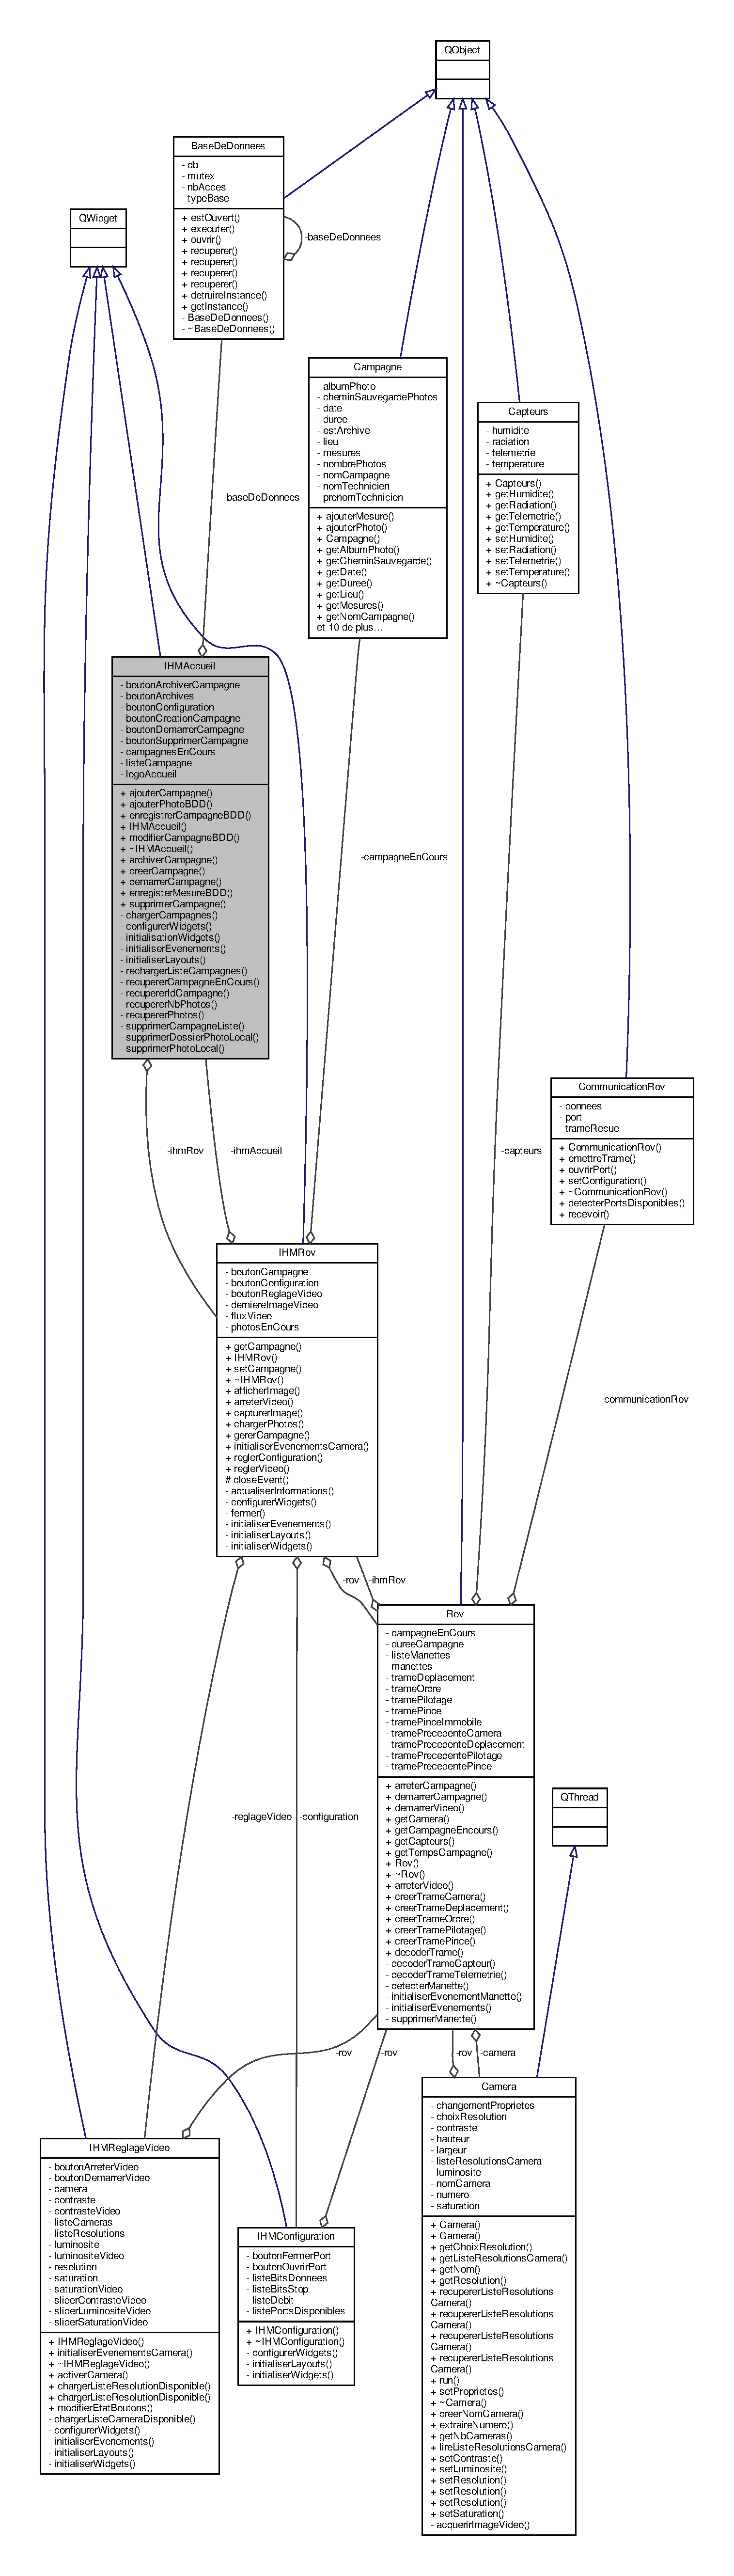
\includegraphics[height=550pt]{class_i_h_m_accueil__coll__graph}
\end{center}
\end{figure}
\subsubsection*{Connecteurs publics}
\begin{DoxyCompactItemize}
\item 
void \hyperlink{class_i_h_m_accueil_a5d38917dbe88751ee966834e1f6c558e}{archiver\+Campagne} ()
\begin{DoxyCompactList}\small\item\em Permet d\textquotesingle{}archiver la campagne selectionner. \end{DoxyCompactList}\item 
void \hyperlink{class_i_h_m_accueil_a1da45b17d6e4198f87a9a0e05d1f7fd5}{creer\+Campagne} ()
\begin{DoxyCompactList}\small\item\em Permet de créer une nouvelle campagne. \end{DoxyCompactList}\item 
void \hyperlink{class_i_h_m_accueil_a6e8935ff4e0ba8f0c0015f370d91eda3}{demarrer\+Campagne} ()
\begin{DoxyCompactList}\small\item\em Permet de démarrer ou reprendre une campagne non archivé \end{DoxyCompactList}\item 
void \hyperlink{class_i_h_m_accueil_af61976178829ec1fc756bec7eff0354d}{enregister\+Mesure\+B\+DD} (Q\+String temperature, Q\+String humidite, Q\+String radiation)
\begin{DoxyCompactList}\small\item\em enregistre les mesures recues dans la base de données \end{DoxyCompactList}\item 
void \hyperlink{class_i_h_m_accueil_a0d7c77277fe83ad13beee56d96c5c5ca}{supprimer\+Campagne} ()
\begin{DoxyCompactList}\small\item\em Permet d\textquotesingle{}archiver la campagne dans la base de données. \end{DoxyCompactList}\end{DoxyCompactItemize}
\subsubsection*{Fonctions membres publiques}
\begin{DoxyCompactItemize}
\item 
void \hyperlink{class_i_h_m_accueil_a3087ce7a78561c79ce3148761750dd1d}{ajouter\+Campagne} (\hyperlink{class_campagne}{Campagne} $\ast$campagne, bool verification=false)
\begin{DoxyCompactList}\small\item\em Ajoute une nouvelle campagne dans la liste des campagne non archivés. \end{DoxyCompactList}\item 
void \hyperlink{class_i_h_m_accueil_aa27c7334efe44c8c4cd582df6581fdff}{ajouter\+Photo\+B\+DD} (\hyperlink{struct_photo}{Photo} \&photo, \hyperlink{class_campagne}{Campagne} $\ast$campagne)
\begin{DoxyCompactList}\small\item\em Ajoute la photo prise dans la B\+DD associé a la campagne. \end{DoxyCompactList}\item 
void \hyperlink{class_i_h_m_accueil_a5ab04fc3fa87817bec130f377d563b75}{enregistrer\+Campagne\+B\+DD} (\hyperlink{class_campagne}{Campagne} $\ast$campagne)
\begin{DoxyCompactList}\small\item\em Enregistre les informations de la campagne dans la B\+DD. \end{DoxyCompactList}\item 
\hyperlink{class_i_h_m_accueil_a66cf4d5655e3132c1d313b76f3905e52}{I\+H\+M\+Accueil} (\hyperlink{class_q_widget}{Q\+Widget} $\ast$parent=nullptr)
\begin{DoxyCompactList}\small\item\em Constructeur de la classe \hyperlink{class_i_h_m_accueil}{I\+H\+M\+Accueil}. \end{DoxyCompactList}\item 
void \hyperlink{class_i_h_m_accueil_a7f1e5f71843a99cb44e3efb7191a6d07}{modifier\+Campagne\+B\+DD} (\hyperlink{class_campagne}{Campagne} $\ast$campagne)
\begin{DoxyCompactList}\small\item\em Met à jour les informations de la campagne lors de l\textquotesingle{}arret de celle-\/ci dans la B\+DD. \end{DoxyCompactList}\item 
\hyperlink{class_i_h_m_accueil_a5ea3926747dada8b9677ab9a33c03139}{$\sim$\+I\+H\+M\+Accueil} ()
\begin{DoxyCompactList}\small\item\em Destructeur de la classe \hyperlink{class_i_h_m_accueil}{I\+H\+M\+Accueil}. \end{DoxyCompactList}\end{DoxyCompactItemize}
\subsubsection*{Fonctions membres privées}
\begin{DoxyCompactItemize}
\item 
void \hyperlink{class_i_h_m_accueil_a1ed3efefdf929c0d2a6b6d1bb10bbc27}{charger\+Campagnes} ()
\begin{DoxyCompactList}\small\item\em Récupere la liste des noms de campagne non terminés et ajoute les nom de la liste des campagnes disponibles. \end{DoxyCompactList}\item 
void \hyperlink{class_i_h_m_accueil_a63bc796a325066423ed6146b8bab1437}{configurer\+Widgets} ()
\begin{DoxyCompactList}\small\item\em Configure les widgets de l\textquotesingle{}I\+HM. \end{DoxyCompactList}\item 
void \hyperlink{class_i_h_m_accueil_a1385a94c1a3d75d813429dc9bdc4b050}{initialisation\+Widgets} ()
\begin{DoxyCompactList}\small\item\em Initialise les widgets de l\textquotesingle{}I\+HM. \end{DoxyCompactList}\item 
void \hyperlink{class_i_h_m_accueil_a5a571ab8f264c275580501753bb00674}{initialiser\+Evenements} ()
\begin{DoxyCompactList}\small\item\em Initialise les evenements de l\textquotesingle{}I\+HM. \end{DoxyCompactList}\item 
void \hyperlink{class_i_h_m_accueil_acaaa5d756165801403ea7d73ae40186b}{initialiser\+Layouts} ()
\begin{DoxyCompactList}\small\item\em Initialise les layouts de l\textquotesingle{}I\+HM. \end{DoxyCompactList}\item 
void \hyperlink{class_i_h_m_accueil_a44074f2d8d59e0d1b7a3d50c24d2a0df}{recharger\+Liste\+Campagnes} ()
\begin{DoxyCompactList}\small\item\em Recharge la liste des campagnes en cours. \end{DoxyCompactList}\item 
void \hyperlink{class_i_h_m_accueil_a0ffb0f0c7c9c613083933514690f2772}{recuperer\+Campagne\+En\+Cours} (bool \&retour\+Campagne, Q\+String \&requete\+Informations\+Campagne, Q\+Vector$<$ Q\+String\+List $>$ \&\hyperlink{class_i_h_m_accueil_ad3827b81480eb201b5927c16a2ad1c46}{campagnes\+En\+Cours})
\begin{DoxyCompactList}\small\item\em Récupère les campagnes en cours dans la base de données, le paramètre campagnes\+En\+Cours passé en référence récupère les valeurs. \end{DoxyCompactList}\item 
Q\+String \hyperlink{class_i_h_m_accueil_a5e222617897b2c1f7e032fa851aa1700}{recuperer\+Id\+Campagne} ()
\begin{DoxyCompactList}\small\item\em Recupere l\textquotesingle{}id de la campagne séléctionné dans la liste. \end{DoxyCompactList}\item 
void \hyperlink{class_i_h_m_accueil_aa09878b2e3e3024220291165b5c528a6}{recuperer\+Nb\+Photos} (Q\+String \&nombre\+Photos, Q\+String \&requete\+Nombre\+Photos)
\begin{DoxyCompactList}\small\item\em Récupère le nombre de photos dans la base de données, le paramètre nombre\+Photos passé en référence récupère la valeur. \end{DoxyCompactList}\item 
void \hyperlink{class_i_h_m_accueil_aebeef48b9bc345edd02e5185951c454e}{recuperer\+Photos} (bool \&retour\+Photo, Q\+String \&requete\+Informations\+Photos, Q\+Vector$<$ Q\+String\+List $>$ \&informations\+Photos)
\begin{DoxyCompactList}\small\item\em Récupère les photos associés a une campagne dans la base de données, le paramètre informations\+Photos passé en référence récupère les valeurs. \end{DoxyCompactList}\item 
void \hyperlink{class_i_h_m_accueil_a36ce6ecca4e258562577bab1439e0a96}{supprimer\+Campagne\+Liste} ()
\begin{DoxyCompactList}\small\item\em Permet de supprimer de lq liste la campagne selectionné \end{DoxyCompactList}\item 
void \hyperlink{class_i_h_m_accueil_acb9679f51e140e0bc28d8ac10afd87e9}{supprimer\+Dossier\+Photo\+Local} ()
\begin{DoxyCompactList}\small\item\em Supprime le dossier photo si il est vide. \end{DoxyCompactList}\item 
void \hyperlink{class_i_h_m_accueil_a9dc22241cd0d4a227b8b0bf04c6404fd}{supprimer\+Photo\+Local} (Q\+String requete)
\begin{DoxyCompactList}\small\item\em Selectionne les chemin d\textquotesingle{}accès des photo à supprimer dans la base de données et les supprime en local. \end{DoxyCompactList}\end{DoxyCompactItemize}
\subsubsection*{Attributs privés}
\begin{DoxyCompactItemize}
\item 
\hyperlink{class_base_de_donnees}{Base\+De\+Donnees} $\ast$ \hyperlink{class_i_h_m_accueil_ab56d9846c071396a92f88272880e2c1f}{base\+De\+Donnees}
\begin{DoxyCompactList}\small\item\em Instance d\textquotesingle{}un objet \hyperlink{class_base_de_donnees}{Base\+De\+Donnees} permettant d\textquotesingle{}acceder a la B\+DD. \end{DoxyCompactList}\item 
Q\+Push\+Button $\ast$ \hyperlink{class_i_h_m_accueil_a96d64cf254c0645eb45c317858b0a0f3}{bouton\+Archiver\+Campagne}
\begin{DoxyCompactList}\small\item\em Bouton permettant d\textquotesingle{}archiver la campagne sélectionner. \end{DoxyCompactList}\item 
Q\+Push\+Button $\ast$ \hyperlink{class_i_h_m_accueil_a313a8c52763aa2978010db77ec6673ac}{bouton\+Archives}
\begin{DoxyCompactList}\small\item\em Bouton permettant d\textquotesingle{}accéder aux archives. \end{DoxyCompactList}\item 
Q\+Push\+Button $\ast$ \hyperlink{class_i_h_m_accueil_a8b8ed7d11ab66e3c6895b3c6129dc9c8}{bouton\+Configuration}
\begin{DoxyCompactList}\small\item\em Bouton permettant de configurer le matériel. \end{DoxyCompactList}\item 
Q\+Push\+Button $\ast$ \hyperlink{class_i_h_m_accueil_a4186b4ef6a9c63f5b3c6431626ff3268}{bouton\+Creation\+Campagne}
\begin{DoxyCompactList}\small\item\em Bouton permettant de créer une nouvelle campagne. \end{DoxyCompactList}\item 
Q\+Push\+Button $\ast$ \hyperlink{class_i_h_m_accueil_a9fd8ab3abc0c1e6addd70c8d7c46fb65}{bouton\+Demarrer\+Campagne}
\begin{DoxyCompactList}\small\item\em Bouton permettant de démarrer ou reprendre la campagne seléctionner. \end{DoxyCompactList}\item 
Q\+Push\+Button $\ast$ \hyperlink{class_i_h_m_accueil_afb409fb4395372f35f9f8699fcb4c89b}{bouton\+Supprimer\+Campagne}
\begin{DoxyCompactList}\small\item\em Bouton permettant de supprimmer la campagne sélectionner. \end{DoxyCompactList}\item 
Q\+Vector$<$ \hyperlink{class_campagne}{Campagne} $\ast$ $>$ \hyperlink{class_i_h_m_accueil_ad3827b81480eb201b5927c16a2ad1c46}{campagnes\+En\+Cours}
\begin{DoxyCompactList}\small\item\em Conteneur des campagnes non archivés. \end{DoxyCompactList}\item 
\hyperlink{class_i_h_m_rov}{I\+H\+M\+Rov} $\ast$ \hyperlink{class_i_h_m_accueil_af9f2613056b21bdf82e8f54a26146acc}{ihm\+Rov}
\begin{DoxyCompactList}\small\item\em Instance d\textquotesingle{}un objet ihm\+Rov. \end{DoxyCompactList}\item 
Q\+Combo\+Box $\ast$ \hyperlink{class_i_h_m_accueil_afb828a4e06c25afa40341c310cd85b08}{liste\+Campagne}
\begin{DoxyCompactList}\small\item\em Liste des campagnes créer et non archivés. \end{DoxyCompactList}\item 
Q\+Label $\ast$ \hyperlink{class_i_h_m_accueil_a709440124f3307589eee68c517833e6d}{logo\+Accueil}
\begin{DoxyCompactList}\small\item\em Logo de l\textquotesingle{}I\+HM accueil. \end{DoxyCompactList}\end{DoxyCompactItemize}


\subsubsection{Description détaillée}
Class permettant de créer une nouvelle campagne, reprendre une campagne mise en pause, archiver une campagne, supprimer une campagne, accéder à la base de données et configurer le matériel. 

Définition à la ligne \hyperlink{ihmaccueil_8h_source_l00026}{26} du fichier \hyperlink{ihmaccueil_8h_source}{ihmaccueil.\+h}.



\subsubsection{Documentation des constructeurs et destructeur}
\mbox{\Hypertarget{class_i_h_m_accueil_a66cf4d5655e3132c1d313b76f3905e52}\label{class_i_h_m_accueil_a66cf4d5655e3132c1d313b76f3905e52}} 
\index{I\+H\+M\+Accueil@{I\+H\+M\+Accueil}!I\+H\+M\+Accueil@{I\+H\+M\+Accueil}}
\index{I\+H\+M\+Accueil@{I\+H\+M\+Accueil}!I\+H\+M\+Accueil@{I\+H\+M\+Accueil}}
\paragraph{\texorpdfstring{I\+H\+M\+Accueil()}{IHMAccueil()}}
{\footnotesize\ttfamily I\+H\+M\+Accueil\+::\+I\+H\+M\+Accueil (\begin{DoxyParamCaption}\item[{\hyperlink{class_q_widget}{Q\+Widget} $\ast$}]{parent = {\ttfamily nullptr} }\end{DoxyParamCaption})\hspace{0.3cm}{\ttfamily [explicit]}}



Constructeur de la classe \hyperlink{class_i_h_m_accueil}{I\+H\+M\+Accueil}. 


\begin{DoxyParams}{Paramètres}
{\em parent} & \\
\hline
\end{DoxyParams}


Définition à la ligne \hyperlink{ihmaccueil_8cpp_source_l00014}{14} du fichier \hyperlink{ihmaccueil_8cpp_source}{ihmaccueil.\+cpp}.



Références \hyperlink{ihmaccueil_8h_source_l00040}{base\+De\+Donnees}, \hyperlink{ihmaccueil_8cpp_source_l00130}{charger\+Campagnes()}, \hyperlink{ihmaccueil_8cpp_source_l00077}{configurer\+Widgets()}, \hyperlink{basededonnees_8cpp_source_l00031}{Base\+De\+Donnees\+::get\+Instance()}, \hyperlink{ihmaccueil_8h_source_l00041}{ihm\+Rov}, \hyperlink{ihmaccueil_8cpp_source_l00037}{initialisation\+Widgets()}, \hyperlink{ihmaccueil_8cpp_source_l00084}{initialiser\+Evenements()}, \hyperlink{ihmaccueil_8cpp_source_l00049}{initialiser\+Layouts()}, et \hyperlink{ihmaccueil_8cpp_source_l00092}{recharger\+Liste\+Campagnes()}.


\begin{DoxyCode}
00014                                       : \hyperlink{class_q_widget}{QWidget}(parent), \hyperlink{class_i_h_m_accueil_ad3827b81480eb201b5927c16a2ad1c46}{campagnesEnCours}()
00015 \{
00016     qDebug() << Q\_FUNC\_INFO;
00017     \hyperlink{class_i_h_m_accueil_ab56d9846c071396a92f88272880e2c1f}{baseDeDonnees} = \hyperlink{class_base_de_donnees_a58beb2f702f75b257e2e55e25d9f979b}{BaseDeDonnees::getInstance}();
00018 
00019     \hyperlink{class_i_h_m_accueil_a1385a94c1a3d75d813429dc9bdc4b050}{initialisationWidgets}();
00020     \hyperlink{class_i_h_m_accueil_a5a571ab8f264c275580501753bb00674}{initialiserEvenements}();
00021     \hyperlink{class_i_h_m_accueil_acaaa5d756165801403ea7d73ae40186b}{initialiserLayouts}();
00022     \hyperlink{class_i_h_m_accueil_a63bc796a325066423ed6146b8bab1437}{configurerWidgets}();
00023 
00024     \hyperlink{class_i_h_m_accueil_a1ed3efefdf929c0d2a6b6d1bb10bbc27}{chargerCampagnes}();
00025     \hyperlink{class_i_h_m_accueil_a44074f2d8d59e0d1b7a3d50c24d2a0df}{rechargerListeCampagnes}();
00026 
00027     \hyperlink{class_i_h_m_accueil_af9f2613056b21bdf82e8f54a26146acc}{ihmRov} = \textcolor{keyword}{new} \hyperlink{class_i_h_m_rov}{IHMRov}(\textcolor{keyword}{this});
00028     \hyperlink{class_i_h_m_accueil_af9f2613056b21bdf82e8f54a26146acc}{ihmRov}->hide();
00029 \}
\end{DoxyCode}
\mbox{\Hypertarget{class_i_h_m_accueil_a5ea3926747dada8b9677ab9a33c03139}\label{class_i_h_m_accueil_a5ea3926747dada8b9677ab9a33c03139}} 
\index{I\+H\+M\+Accueil@{I\+H\+M\+Accueil}!````~I\+H\+M\+Accueil@{$\sim$\+I\+H\+M\+Accueil}}
\index{````~I\+H\+M\+Accueil@{$\sim$\+I\+H\+M\+Accueil}!I\+H\+M\+Accueil@{I\+H\+M\+Accueil}}
\paragraph{\texorpdfstring{$\sim$\+I\+H\+M\+Accueil()}{~IHMAccueil()}}
{\footnotesize\ttfamily I\+H\+M\+Accueil\+::$\sim$\+I\+H\+M\+Accueil (\begin{DoxyParamCaption}{ }\end{DoxyParamCaption})}



Destructeur de la classe \hyperlink{class_i_h_m_accueil}{I\+H\+M\+Accueil}. 



Définition à la ligne \hyperlink{ihmaccueil_8cpp_source_l00031}{31} du fichier \hyperlink{ihmaccueil_8cpp_source}{ihmaccueil.\+cpp}.



Références \hyperlink{basededonnees_8cpp_source_l00044}{Base\+De\+Donnees\+::detruire\+Instance()}.


\begin{DoxyCode}
00032 \{
00033     \hyperlink{class_base_de_donnees_a457401c0816b888c77ce915997545f4e}{BaseDeDonnees::detruireInstance}();
00034     qDebug() << Q\_FUNC\_INFO;
00035 \}
\end{DoxyCode}


\subsubsection{Documentation des fonctions membres}
\mbox{\Hypertarget{class_i_h_m_accueil_a3087ce7a78561c79ce3148761750dd1d}\label{class_i_h_m_accueil_a3087ce7a78561c79ce3148761750dd1d}} 
\index{I\+H\+M\+Accueil@{I\+H\+M\+Accueil}!ajouter\+Campagne@{ajouter\+Campagne}}
\index{ajouter\+Campagne@{ajouter\+Campagne}!I\+H\+M\+Accueil@{I\+H\+M\+Accueil}}
\paragraph{\texorpdfstring{ajouter\+Campagne()}{ajouterCampagne()}}
{\footnotesize\ttfamily void I\+H\+M\+Accueil\+::ajouter\+Campagne (\begin{DoxyParamCaption}\item[{\hyperlink{class_campagne}{Campagne} $\ast$}]{campagne,  }\item[{bool}]{verification = {\ttfamily false} }\end{DoxyParamCaption})}



Ajoute une nouvelle campagne dans la liste des campagne non archivés. 


\begin{DoxyParams}{Paramètres}
{\em campagne} & \\
\hline
{\em verification} & \\
\hline
\end{DoxyParams}


Définition à la ligne \hyperlink{ihmaccueil_8cpp_source_l00254}{254} du fichier \hyperlink{ihmaccueil_8cpp_source}{ihmaccueil.\+cpp}.



Références \hyperlink{ihmaccueil_8h_source_l00039}{campagnes\+En\+Cours}, \hyperlink{campagne_8cpp_source_l00055}{Campagne\+::get\+Chemin\+Sauvegarde()}, \hyperlink{campagne_8cpp_source_l00019}{Campagne\+::get\+Nom\+Campagne()}, et \hyperlink{ihmaccueil_8cpp_source_l00092}{recharger\+Liste\+Campagnes()}.



Référencé par \hyperlink{ihmaccueil_8cpp_source_l00130}{charger\+Campagnes()}, et \hyperlink{ihmcreationcampagne_8cpp_source_l00071}{I\+H\+M\+Creation\+Campagne\+::valider\+Campagne()}.


\begin{DoxyCode}
00255 \{
00256     QDir dossierCampagne(campagne->\hyperlink{class_campagne_ad752790357417d83a93056d9c9689a16}{getCheminSauvegarde}());
00257     \textcolor{keywordflow}{if}(dossierCampagne.exists())
00258     \{
00259         \textcolor{keywordflow}{if}(!dossierCampagne.mkdir(campagne->\hyperlink{class_campagne_a99a682fcb8e5a3f8c2aff7a44eb2c930}{getNomCampagne}()))
00260         \{
00261             qDebug() << Q\_FUNC\_INFO << \textcolor{stringliteral}{"Erreur : impossible de créer le dossier"} << campagne->
      \hyperlink{class_campagne_ad752790357417d83a93056d9c9689a16}{getCheminSauvegarde}() << \textcolor{stringliteral}{"campagne"} << campagne->
      \hyperlink{class_campagne_a99a682fcb8e5a3f8c2aff7a44eb2c930}{getNomCampagne}();
00262             \textcolor{keywordflow}{if}(verification)
00263             \{
00264                 QMessageBox::critical(\textcolor{keyword}{this}, \textcolor{stringliteral}{"Erreur"}, \textcolor{stringliteral}{"Erreur : impossible de créer le dossier "} + campagne
      ->\hyperlink{class_campagne_ad752790357417d83a93056d9c9689a16}{getCheminSauvegarde}() + \textcolor{stringliteral}{" !"});
00265                 \textcolor{keywordflow}{return};
00266             \}
00267         \}
00268     \}
00269     \hyperlink{class_i_h_m_accueil_ad3827b81480eb201b5927c16a2ad1c46}{campagnesEnCours}.push\_back(campagne);
00270     \hyperlink{class_i_h_m_accueil_a44074f2d8d59e0d1b7a3d50c24d2a0df}{rechargerListeCampagnes}();
00271 \}
\end{DoxyCode}
\mbox{\Hypertarget{class_i_h_m_accueil_aa27c7334efe44c8c4cd582df6581fdff}\label{class_i_h_m_accueil_aa27c7334efe44c8c4cd582df6581fdff}} 
\index{I\+H\+M\+Accueil@{I\+H\+M\+Accueil}!ajouter\+Photo\+B\+DD@{ajouter\+Photo\+B\+DD}}
\index{ajouter\+Photo\+B\+DD@{ajouter\+Photo\+B\+DD}!I\+H\+M\+Accueil@{I\+H\+M\+Accueil}}
\paragraph{\texorpdfstring{ajouter\+Photo\+B\+D\+D()}{ajouterPhotoBDD()}}
{\footnotesize\ttfamily void I\+H\+M\+Accueil\+::ajouter\+Photo\+B\+DD (\begin{DoxyParamCaption}\item[{\hyperlink{struct_photo}{Photo} \&}]{photo,  }\item[{\hyperlink{class_campagne}{Campagne} $\ast$}]{campagne }\end{DoxyParamCaption})}



Ajoute la photo prise dans la B\+DD associé a la campagne. 


\begin{DoxyParams}{Paramètres}
{\em photo} & \\
\hline
{\em campagne} & \\
\hline
\end{DoxyParams}


Définition à la ligne \hyperlink{ihmaccueil_8cpp_source_l00313}{313} du fichier \hyperlink{ihmaccueil_8cpp_source}{ihmaccueil.\+cpp}.



Références \hyperlink{ihmaccueil_8h_source_l00040}{base\+De\+Donnees}, \hyperlink{ihmalbumphoto_8h_source_l00025}{Photo\+::chemin\+Sauvegarde}, \hyperlink{basededonnees_8cpp_source_l00104}{Base\+De\+Donnees\+::executer()}, \hyperlink{campagne_8cpp_source_l00019}{Campagne\+::get\+Nom\+Campagne()}, et \hyperlink{basededonnees_8cpp_source_l00139}{Base\+De\+Donnees\+::recuperer()}.



Référencé par \hyperlink{ihmrov_8cpp_source_l00179}{I\+H\+M\+Rov\+::capturer\+Image()}.


\begin{DoxyCode}
00314 \{
00315     QString idCampagne;
00316     QString requeteIdCampagne = \textcolor{stringliteral}{"SELECT IdCampagne FROM campagne WHERE campagne.nom = '"} + campagne->
      \hyperlink{class_campagne_a99a682fcb8e5a3f8c2aff7a44eb2c930}{getNomCampagne}() + \textcolor{stringliteral}{"'"};
00317     \hyperlink{class_i_h_m_accueil_ab56d9846c071396a92f88272880e2c1f}{baseDeDonnees}->\hyperlink{class_base_de_donnees_a77539baad389f5acf754cd2cd452403e}{recuperer}(requeteIdCampagne, idCampagne);
00318 
00319     QString requeteInsertion = \textcolor{stringliteral}{"INSERT INTO photo (idCampagne, cheminImage, aGarder) VALUES ('"} + 
      idCampagne + \textcolor{stringliteral}{"', '"} + photo.\hyperlink{struct_photo_a3c28eb9ad160b65deb46a72146a1d14f}{cheminSauvegarde} + \textcolor{stringliteral}{"', '1')"};
00320     \hyperlink{class_i_h_m_accueil_ab56d9846c071396a92f88272880e2c1f}{baseDeDonnees}->\hyperlink{class_base_de_donnees_aa8de5f8f8bb17edc43f5c0ee33712081}{executer}(requeteInsertion);
00321 \}
\end{DoxyCode}
\mbox{\Hypertarget{class_i_h_m_accueil_a5d38917dbe88751ee966834e1f6c558e}\label{class_i_h_m_accueil_a5d38917dbe88751ee966834e1f6c558e}} 
\index{I\+H\+M\+Accueil@{I\+H\+M\+Accueil}!archiver\+Campagne@{archiver\+Campagne}}
\index{archiver\+Campagne@{archiver\+Campagne}!I\+H\+M\+Accueil@{I\+H\+M\+Accueil}}
\paragraph{\texorpdfstring{archiver\+Campagne}{archiverCampagne}}
{\footnotesize\ttfamily void I\+H\+M\+Accueil\+::archiver\+Campagne (\begin{DoxyParamCaption}{ }\end{DoxyParamCaption})\hspace{0.3cm}{\ttfamily [slot]}}



Permet d\textquotesingle{}archiver la campagne selectionner. 



Définition à la ligne \hyperlink{ihmaccueil_8cpp_source_l00350}{350} du fichier \hyperlink{ihmaccueil_8cpp_source}{ihmaccueil.\+cpp}.



Références \hyperlink{ihmaccueil_8h_source_l00040}{base\+De\+Donnees}, \hyperlink{basededonnees_8cpp_source_l00104}{Base\+De\+Donnees\+::executer()}, \hyperlink{ihmaccueil_8h_source_l00037}{liste\+Campagne}, \hyperlink{basededonnees_8cpp_source_l00063}{Base\+De\+Donnees\+::ouvrir()}, \hyperlink{ihmaccueil_8cpp_source_l00205}{recuperer\+Id\+Campagne()}, \hyperlink{ihmaccueil_8cpp_source_l00189}{supprimer\+Campagne\+Liste()}, et \hyperlink{ihmaccueil_8cpp_source_l00224}{supprimer\+Photo\+Local()}.



Référencé par \hyperlink{ihmaccueil_8cpp_source_l00084}{initialiser\+Evenements()}.


\begin{DoxyCode}
00351 \{
00352     \hyperlink{class_i_h_m_accueil_ab56d9846c071396a92f88272880e2c1f}{baseDeDonnees}->\hyperlink{class_base_de_donnees_a7f6a5510b08017b0d99115a84252f186}{ouvrir}(\textcolor{stringliteral}{"campagnes.sqlite"});
00353     \textcolor{keywordtype}{bool} retourRequeteArchiver;
00354     \textcolor{keywordtype}{bool} retourRequeteSuppressionPhoto;
00355     QString requeteArchiver, requeteSuppressionPhoto;
00356 
00357     \hyperlink{class_i_h_m_accueil_a9dc22241cd0d4a227b8b0bf04c6404fd}{supprimerPhotoLocal}(\textcolor{stringliteral}{"SELECT photo.cheminImage FROM photo WHERE photo.IdCampagne = '"}
       + \hyperlink{class_i_h_m_accueil_a5e222617897b2c1f7e032fa851aa1700}{recupererIdCampagne}() + \textcolor{stringliteral}{"' AND photo.aGarder = '0'"});
00358 
00359     requeteArchiver = \textcolor{stringliteral}{"UPDATE campagne SET enCours = '0' WHERE campagne.nom = '"} + 
      \hyperlink{class_i_h_m_accueil_afb828a4e06c25afa40341c310cd85b08}{listeCampagne}->currentText() + \textcolor{stringliteral}{"'"};
00360     requeteSuppressionPhoto = \textcolor{stringliteral}{"DELETE FROM photo WHERE photo.IdCampagne = '"} + 
      \hyperlink{class_i_h_m_accueil_a5e222617897b2c1f7e032fa851aa1700}{recupererIdCampagne}() + \textcolor{stringliteral}{"' AND photo.aGarder = '0'"};
00361 
00362     retourRequeteArchiver = \hyperlink{class_i_h_m_accueil_ab56d9846c071396a92f88272880e2c1f}{baseDeDonnees}->\hyperlink{class_base_de_donnees_aa8de5f8f8bb17edc43f5c0ee33712081}{executer}(requeteArchiver);
00363     retourRequeteSuppressionPhoto = \hyperlink{class_i_h_m_accueil_ab56d9846c071396a92f88272880e2c1f}{baseDeDonnees}->\hyperlink{class_base_de_donnees_aa8de5f8f8bb17edc43f5c0ee33712081}{executer}(requeteSuppressionPhoto);
00364 
00365     \textcolor{keywordflow}{if}(!retourRequeteArchiver && !retourRequeteSuppressionPhoto)
00366     \{
00367 \textcolor{preprocessor}{        #ifdef DEBUG\_BASEDEDONNEES}
00368             qDebug() << Q\_FUNC\_INFO << QString::fromUtf8(\textcolor{stringliteral}{"erreur !"});
00369 \textcolor{preprocessor}{        #endif}
00370     \}
00371     \textcolor{keywordflow}{else}
00372         \hyperlink{class_i_h_m_accueil_a36ce6ecca4e258562577bab1439e0a96}{supprimerCampagneListe}();
00373 \}
\end{DoxyCode}
\mbox{\Hypertarget{class_i_h_m_accueil_a1ed3efefdf929c0d2a6b6d1bb10bbc27}\label{class_i_h_m_accueil_a1ed3efefdf929c0d2a6b6d1bb10bbc27}} 
\index{I\+H\+M\+Accueil@{I\+H\+M\+Accueil}!charger\+Campagnes@{charger\+Campagnes}}
\index{charger\+Campagnes@{charger\+Campagnes}!I\+H\+M\+Accueil@{I\+H\+M\+Accueil}}
\paragraph{\texorpdfstring{charger\+Campagnes()}{chargerCampagnes()}}
{\footnotesize\ttfamily void I\+H\+M\+Accueil\+::charger\+Campagnes (\begin{DoxyParamCaption}{ }\end{DoxyParamCaption})\hspace{0.3cm}{\ttfamily [private]}}



Récupere la liste des noms de campagne non terminés et ajoute les nom de la liste des campagnes disponibles. 



Définition à la ligne \hyperlink{ihmaccueil_8cpp_source_l00130}{130} du fichier \hyperlink{ihmaccueil_8cpp_source}{ihmaccueil.\+cpp}.



Références \hyperlink{ihmalbumphoto_8h_source_l00024}{Photo\+::a\+Garder}, \hyperlink{ihmaccueil_8cpp_source_l00254}{ajouter\+Campagne()}, \hyperlink{campagne_8cpp_source_l00080}{Campagne\+::ajouter\+Photo()}, \hyperlink{ihmaccueil_8h_source_l00040}{base\+De\+Donnees}, \hyperlink{ihmaccueil_8h_source_l00039}{campagnes\+En\+Cours}, \hyperlink{ihmalbumphoto_8h_source_l00025}{Photo\+::chemin\+Sauvegarde}, \hyperlink{ihmalbumphoto_8h_source_l00022}{Photo\+::image}, \hyperlink{basededonnees_8cpp_source_l00063}{Base\+De\+Donnees\+::ouvrir()}, \hyperlink{ihmaccueil_8cpp_source_l00120}{recuperer\+Campagne\+En\+Cours()}, \hyperlink{ihmaccueil_8cpp_source_l00115}{recuperer\+Nb\+Photos()}, \hyperlink{ihmaccueil_8cpp_source_l00125}{recuperer\+Photos()}, \hyperlink{campagne_8cpp_source_l00060}{Campagne\+::set\+Chemin\+Sauvegarde()}, et \hyperlink{campagne_8cpp_source_l00065}{Campagne\+::set\+Nombre\+Photos()}.



Référencé par \hyperlink{ihmaccueil_8cpp_source_l00014}{I\+H\+M\+Accueil()}.


\begin{DoxyCode}
00131 \{
00132     \hyperlink{class_i_h_m_accueil_ab56d9846c071396a92f88272880e2c1f}{baseDeDonnees}->\hyperlink{class_base_de_donnees_a7f6a5510b08017b0d99115a84252f186}{ouvrir}(\textcolor{stringliteral}{"campagnes.sqlite"});
00133 
00134     \textcolor{keywordtype}{bool} retourCampagne, retourPhoto;
00135     QVector<QStringList> \hyperlink{class_i_h_m_accueil_ad3827b81480eb201b5927c16a2ad1c46}{campagnesEnCours};
00136     QString nombrePhotos;
00137     QVector<QStringList> informationsPhotos;
00138 
00139     QString requeteInformationsCampagne = \textcolor{stringliteral}{"SELECT campagne.idCampagne, campagne.nom, campagne.lieu,
       technicien.nom, technicien.prenom, campagne.date, campagne.duree, campagne.cheminSauvegarde FROM campagne INNER
       JOIN technicien ON campagne.idTechnicien = technicien.idTechnicien WHERE campagne.enCours = '1' ORDER BY
       campagne.date DESC"};
00140 
00141 \textcolor{preprocessor}{    #ifdef DEBUG\_BASEDEDONNEES}
00142     qDebug() << Q\_FUNC\_INFO << QString::fromUtf8(\textcolor{stringliteral}{"requête : "}) << requeteInformationsCampagne;
00143 \textcolor{preprocessor}{    #endif}
00144 
00145     \hyperlink{class_i_h_m_accueil_a0ffb0f0c7c9c613083933514690f2772}{recupererCampagneEnCours}(retourCampagne, requeteInformationsCampagne, 
      campagnesEnCours);
00146     \textcolor{keywordflow}{if}(retourCampagne)
00147     \{
00148         \textcolor{keywordflow}{for}(\textcolor{keywordtype}{int} i=0; i < campagnesEnCours.size(); i++)
00149         \{
00150             QStringList informationsCampagne = campagnesEnCours.at(i);
00151             QString requeteNombrePhotos = \textcolor{stringliteral}{"SELECT COUNT(IdPhoto) FROM photo INNER JOIN campagne ON
       photo.IdCampagne = campagne.IdCampagne WHERE campagne.IdCampagne = '"} + informationsCampagne.at(0) + \textcolor{stringliteral}{"' "};
00152             \hyperlink{class_i_h_m_accueil_aa09878b2e3e3024220291165b5c528a6}{recupererNbPhotos}(nombrePhotos, requeteNombrePhotos);
00153 
00154 \textcolor{preprocessor}{            #ifdef DEBUG\_BASEDEDONNEES}
00155             qDebug() << Q\_FUNC\_INFO << QString::fromUtf8(\textcolor{stringliteral}{"%0 %1 %2 %3 %4 %5 %6 %7"}).arg(
      informationsCampagne.at(0)).arg(informationsCampagne.at(1)).arg(informationsCampagne.at(2)).arg(informationsCampagne.at(3)).arg
      (informationsCampagne.at(4)).arg(informationsCampagne.at(5)).arg(informationsCampagne.at(6)).arg(
      informationsCampagne.at(7));
00156 \textcolor{preprocessor}{            #endif}
00157             \hyperlink{class_campagne}{Campagne} *campagne = \textcolor{keyword}{new} \hyperlink{class_campagne}{Campagne}(informationsCampagne.at(1), 
      informationsCampagne.at(2), informationsCampagne.at(3), informationsCampagne.at(4), QDateTime::fromString(
      informationsCampagne.at(5)), \textcolor{keyword}{this}, informationsCampagne.at(6).toInt());
00158 
00159             campagne->\hyperlink{class_campagne_a68c7eb6776e46306b10f1ca2a409ae6e}{setCheminSauvegarde}(informationsCampagne.at(7));
00160             campagne->\hyperlink{class_campagne_a2b8848ade0f97708571331ef71e4c9cb}{setNombrePhotos}(nombrePhotos.toInt());
00161 
00162             QString requeteInformationsPhotos =\textcolor{stringliteral}{"SELECT cheminImage, aGarder FROM photo INNER JOIN campagne
       ON photo.IdCampagne = campagne.IdCampagne WHERE campagne.enCours = '1' AND photo.IdCampagne = '"} + 
      informationsCampagne.at(0) + \textcolor{stringliteral}{"'"};
00163             \hyperlink{class_i_h_m_accueil_aebeef48b9bc345edd02e5185951c454e}{recupererPhotos}(retourPhoto, requeteInformationsPhotos, informationsPhotos);
00164             \textcolor{keywordflow}{if}(retourPhoto)
00165             \{
00166                 \textcolor{keywordflow}{for}(\textcolor{keywordtype}{int} i=0; i < informationsPhotos.size(); i++)
00167                 \{
00168                     QStringList informationPhoto = informationsPhotos.at(i);
00169                     \hyperlink{struct_photo}{Photo} photo;
00170                     photo.\hyperlink{struct_photo_a3c28eb9ad160b65deb46a72146a1d14f}{cheminSauvegarde} = informationPhoto.at(0);
00171                     photo.\hyperlink{struct_photo_afec1baefdd7d036432494bbb33b21366}{aGarder} = informationPhoto.at(1).toInt();
00172                     photo.\hyperlink{struct_photo_aa6ecfed8082bea5af2905208308a6adb}{image} = QPixmap(informationPhoto.at(0));
00173 
00174                     campagne->\hyperlink{class_campagne_a472029bf46646d136a750dbaa7a3155f}{ajouterPhoto}(photo);
00175                 \}
00176             \}
00177             \hyperlink{class_i_h_m_accueil_a3087ce7a78561c79ce3148761750dd1d}{ajouterCampagne}(campagne);
00178             informationsPhotos.clear();
00179         \}
00180      \}
00181      \textcolor{keywordflow}{else}
00182      \{
00183 \textcolor{preprocessor}{        #ifdef DEBUG\_BASEDEDONNEES}
00184         qDebug() << Q\_FUNC\_INFO << QString::fromUtf8(\textcolor{stringliteral}{"erreur !"});
00185 \textcolor{preprocessor}{        #endif}
00186      \}
00187 \}
\end{DoxyCode}
\mbox{\Hypertarget{class_i_h_m_accueil_a63bc796a325066423ed6146b8bab1437}\label{class_i_h_m_accueil_a63bc796a325066423ed6146b8bab1437}} 
\index{I\+H\+M\+Accueil@{I\+H\+M\+Accueil}!configurer\+Widgets@{configurer\+Widgets}}
\index{configurer\+Widgets@{configurer\+Widgets}!I\+H\+M\+Accueil@{I\+H\+M\+Accueil}}
\paragraph{\texorpdfstring{configurer\+Widgets()}{configurerWidgets()}}
{\footnotesize\ttfamily void I\+H\+M\+Accueil\+::configurer\+Widgets (\begin{DoxyParamCaption}{ }\end{DoxyParamCaption})\hspace{0.3cm}{\ttfamily [private]}}



Configure les widgets de l\textquotesingle{}I\+HM. 



Définition à la ligne \hyperlink{ihmaccueil_8cpp_source_l00077}{77} du fichier \hyperlink{ihmaccueil_8cpp_source}{ihmaccueil.\+cpp}.



Références \hyperlink{ihmaccueil_8h_source_l00037}{liste\+Campagne}, et \hyperlink{ihmaccueil_8h_source_l00038}{logo\+Accueil}.



Référencé par \hyperlink{ihmaccueil_8cpp_source_l00014}{I\+H\+M\+Accueil()}.


\begin{DoxyCode}
00078 \{
00079     qDebug() << Q\_FUNC\_INFO << qApp->applicationDirPath() + \textcolor{stringliteral}{"/images/Robot.png"};
00080     \hyperlink{class_i_h_m_accueil_a709440124f3307589eee68c517833e6d}{logoAccueil}->setPixmap(QPixmap(qApp->applicationDirPath() + \textcolor{stringliteral}{"/images/Robot.png"}));
00081     \hyperlink{class_i_h_m_accueil_afb828a4e06c25afa40341c310cd85b08}{listeCampagne}->setEditable(\textcolor{keyword}{false});
00082 \}
\end{DoxyCode}
\mbox{\Hypertarget{class_i_h_m_accueil_a1da45b17d6e4198f87a9a0e05d1f7fd5}\label{class_i_h_m_accueil_a1da45b17d6e4198f87a9a0e05d1f7fd5}} 
\index{I\+H\+M\+Accueil@{I\+H\+M\+Accueil}!creer\+Campagne@{creer\+Campagne}}
\index{creer\+Campagne@{creer\+Campagne}!I\+H\+M\+Accueil@{I\+H\+M\+Accueil}}
\paragraph{\texorpdfstring{creer\+Campagne}{creerCampagne}}
{\footnotesize\ttfamily void I\+H\+M\+Accueil\+::creer\+Campagne (\begin{DoxyParamCaption}{ }\end{DoxyParamCaption})\hspace{0.3cm}{\ttfamily [slot]}}



Permet de créer une nouvelle campagne. 



Définition à la ligne \hyperlink{ihmaccueil_8cpp_source_l00339}{339} du fichier \hyperlink{ihmaccueil_8cpp_source}{ihmaccueil.\+cpp}.



Références \hyperlink{ihmaccueil_8h_source_l00040}{base\+De\+Donnees}, et \hyperlink{basededonnees_8cpp_source_l00139}{Base\+De\+Donnees\+::recuperer()}.



Référencé par \hyperlink{ihmaccueil_8cpp_source_l00084}{initialiser\+Evenements()}.


\begin{DoxyCode}
00340 \{
00341     QVector<QStringList> listeTechniciens;
00342     QString requete = \textcolor{stringliteral}{"SELECT technicien.nom, technicien.prenom FROM technicien"};
00343 
00344     \hyperlink{class_i_h_m_accueil_ab56d9846c071396a92f88272880e2c1f}{baseDeDonnees}->\hyperlink{class_base_de_donnees_a77539baad389f5acf754cd2cd452403e}{recuperer}(requete, listeTechniciens);
00345 
00346     \hyperlink{class_i_h_m_creation_campagne}{IHMCreationCampagne} *ihmCreationCampagne = \textcolor{keyword}{new} 
      \hyperlink{class_i_h_m_creation_campagne}{IHMCreationCampagne}(\textcolor{keyword}{this}, listeTechniciens);
00347     ihmCreationCampagne->exec();
00348 \}
\end{DoxyCode}
\mbox{\Hypertarget{class_i_h_m_accueil_a6e8935ff4e0ba8f0c0015f370d91eda3}\label{class_i_h_m_accueil_a6e8935ff4e0ba8f0c0015f370d91eda3}} 
\index{I\+H\+M\+Accueil@{I\+H\+M\+Accueil}!demarrer\+Campagne@{demarrer\+Campagne}}
\index{demarrer\+Campagne@{demarrer\+Campagne}!I\+H\+M\+Accueil@{I\+H\+M\+Accueil}}
\paragraph{\texorpdfstring{demarrer\+Campagne}{demarrerCampagne}}
{\footnotesize\ttfamily void I\+H\+M\+Accueil\+::demarrer\+Campagne (\begin{DoxyParamCaption}{ }\end{DoxyParamCaption})\hspace{0.3cm}{\ttfamily [slot]}}



Permet de démarrer ou reprendre une campagne non archivé 



Définition à la ligne \hyperlink{ihmaccueil_8cpp_source_l00323}{323} du fichier \hyperlink{ihmaccueil_8cpp_source}{ihmaccueil.\+cpp}.



Références \hyperlink{ihmaccueil_8h_source_l00039}{campagnes\+En\+Cours}, \hyperlink{ihmrov_8cpp_source_l00202}{I\+H\+M\+Rov\+::gerer\+Campagne()}, \hyperlink{ihmaccueil_8h_source_l00041}{ihm\+Rov}, \hyperlink{ihmaccueil_8h_source_l00037}{liste\+Campagne}, et \hyperlink{ihmrov_8cpp_source_l00143}{I\+H\+M\+Rov\+::set\+Campagne()}.



Référencé par \hyperlink{ihmaccueil_8cpp_source_l00084}{initialiser\+Evenements()}.


\begin{DoxyCode}
00324 \{
00325     \textcolor{keywordflow}{for}(QVector<Campagne*>::iterator it = \hyperlink{class_i_h_m_accueil_ad3827b81480eb201b5927c16a2ad1c46}{campagnesEnCours}.begin(); it != 
      \hyperlink{class_i_h_m_accueil_ad3827b81480eb201b5927c16a2ad1c46}{campagnesEnCours}.end(); it++)
00326     \{
00327         \textcolor{keywordflow}{if}((*it)->getNomCampagne() == \hyperlink{class_i_h_m_accueil_afb828a4e06c25afa40341c310cd85b08}{listeCampagne}->currentText())
00328         \{
00329             qDebug() << Q\_FUNC\_INFO << \hyperlink{class_i_h_m_accueil_afb828a4e06c25afa40341c310cd85b08}{listeCampagne}->currentText();
00330             \hyperlink{class_i_h_m_accueil_af9f2613056b21bdf82e8f54a26146acc}{ihmRov}->\hyperlink{class_i_h_m_rov_a301a0b8cb323c2c9de71df9070bb7555}{setCampagne}(*it);
00331             \hyperlink{class_i_h_m_accueil_af9f2613056b21bdf82e8f54a26146acc}{ihmRov}->show();
00332             \hyperlink{class_i_h_m_accueil_af9f2613056b21bdf82e8f54a26146acc}{ihmRov}->\hyperlink{class_i_h_m_rov_a3660d3b4bf61367534eae9d0c3618a5e}{gererCampagne}();
00333             this->setVisible(\textcolor{keyword}{false});
00334             \textcolor{keywordflow}{break};
00335         \}
00336     \}    
00337 \}
\end{DoxyCode}
\mbox{\Hypertarget{class_i_h_m_accueil_af61976178829ec1fc756bec7eff0354d}\label{class_i_h_m_accueil_af61976178829ec1fc756bec7eff0354d}} 
\index{I\+H\+M\+Accueil@{I\+H\+M\+Accueil}!enregister\+Mesure\+B\+DD@{enregister\+Mesure\+B\+DD}}
\index{enregister\+Mesure\+B\+DD@{enregister\+Mesure\+B\+DD}!I\+H\+M\+Accueil@{I\+H\+M\+Accueil}}
\paragraph{\texorpdfstring{enregister\+Mesure\+B\+DD}{enregisterMesureBDD}}
{\footnotesize\ttfamily void I\+H\+M\+Accueil\+::enregister\+Mesure\+B\+DD (\begin{DoxyParamCaption}\item[{Q\+String}]{temperature,  }\item[{Q\+String}]{humidite,  }\item[{Q\+String}]{radiation }\end{DoxyParamCaption})\hspace{0.3cm}{\ttfamily [slot]}}



enregistre les mesures recues dans la base de données 


\begin{DoxyParams}{Paramètres}
{\em temperature} & \\
\hline
{\em humidite} & \\
\hline
{\em radiation} & \\
\hline
\end{DoxyParams}


Définition à la ligne \hyperlink{ihmaccueil_8cpp_source_l00404}{404} du fichier \hyperlink{ihmaccueil_8cpp_source}{ihmaccueil.\+cpp}.



Références \hyperlink{ihmaccueil_8h_source_l00040}{base\+De\+Donnees}, \hyperlink{basededonnees_8cpp_source_l00104}{Base\+De\+Donnees\+::executer()}, \hyperlink{basededonnees_8cpp_source_l00063}{Base\+De\+Donnees\+::ouvrir()}, et \hyperlink{ihmaccueil_8cpp_source_l00205}{recuperer\+Id\+Campagne()}.


\begin{DoxyCode}
00405 \{
00406     \hyperlink{class_i_h_m_accueil_ab56d9846c071396a92f88272880e2c1f}{baseDeDonnees}->\hyperlink{class_base_de_donnees_a7f6a5510b08017b0d99115a84252f186}{ouvrir}(\textcolor{stringliteral}{"campagnes.sqlite"});
00407     \textcolor{keywordtype}{bool} retourRequeteEnregistrementMesure;
00408 
00409     QString requeteEnregistrementMesure = \textcolor{stringliteral}{"INSERT INTO mesure (idCampagne, heure, temperature, radiation,
       humidite) VALUES ("} + \hyperlink{class_i_h_m_accueil_a5e222617897b2c1f7e032fa851aa1700}{recupererIdCampagne}() + \textcolor{stringliteral}{","} + QDateTime::currentDateTime().toString(
      ) + \textcolor{stringliteral}{","} + temperature + \textcolor{stringliteral}{","} + humidite + \textcolor{stringliteral}{","} + radiation + \textcolor{stringliteral}{")"};
00410 
00411     retourRequeteEnregistrementMesure = \hyperlink{class_i_h_m_accueil_ab56d9846c071396a92f88272880e2c1f}{baseDeDonnees}->\hyperlink{class_base_de_donnees_aa8de5f8f8bb17edc43f5c0ee33712081}{executer}(
      requeteEnregistrementMesure);
00412 
00413     \textcolor{keywordflow}{if}(!retourRequeteEnregistrementMesure)
00414     \{
00415 \textcolor{preprocessor}{        #ifdef DEBUG\_BASEDEDONNEES}
00416             qDebug() << Q\_FUNC\_INFO << QString::fromUtf8(\textcolor{stringliteral}{"erreur !"});
00417 \textcolor{preprocessor}{        #endif}
00418     \}
00419 \}
\end{DoxyCode}
\mbox{\Hypertarget{class_i_h_m_accueil_a5ab04fc3fa87817bec130f377d563b75}\label{class_i_h_m_accueil_a5ab04fc3fa87817bec130f377d563b75}} 
\index{I\+H\+M\+Accueil@{I\+H\+M\+Accueil}!enregistrer\+Campagne\+B\+DD@{enregistrer\+Campagne\+B\+DD}}
\index{enregistrer\+Campagne\+B\+DD@{enregistrer\+Campagne\+B\+DD}!I\+H\+M\+Accueil@{I\+H\+M\+Accueil}}
\paragraph{\texorpdfstring{enregistrer\+Campagne\+B\+D\+D()}{enregistrerCampagneBDD()}}
{\footnotesize\ttfamily void I\+H\+M\+Accueil\+::enregistrer\+Campagne\+B\+DD (\begin{DoxyParamCaption}\item[{\hyperlink{class_campagne}{Campagne} $\ast$}]{campagne }\end{DoxyParamCaption})}



Enregistre les informations de la campagne dans la B\+DD. 


\begin{DoxyParams}{Paramètres}
{\em campagne} & \\
\hline
\end{DoxyParams}


Définition à la ligne \hyperlink{ihmaccueil_8cpp_source_l00273}{273} du fichier \hyperlink{ihmaccueil_8cpp_source}{ihmaccueil.\+cpp}.



Références \hyperlink{ihmaccueil_8h_source_l00040}{base\+De\+Donnees}, \hyperlink{basededonnees_8cpp_source_l00104}{Base\+De\+Donnees\+::executer()}, \hyperlink{campagne_8cpp_source_l00055}{Campagne\+::get\+Chemin\+Sauvegarde()}, \hyperlink{campagne_8cpp_source_l00039}{Campagne\+::get\+Date()}, \hyperlink{campagne_8cpp_source_l00044}{Campagne\+::get\+Duree()}, \hyperlink{campagne_8cpp_source_l00034}{Campagne\+::get\+Lieu()}, \hyperlink{campagne_8cpp_source_l00019}{Campagne\+::get\+Nom\+Campagne()}, \hyperlink{campagne_8cpp_source_l00024}{Campagne\+::get\+Nom\+Technicien()}, \hyperlink{campagne_8cpp_source_l00029}{Campagne\+::get\+Prenom\+Technicien()}, \hyperlink{basededonnees_8cpp_source_l00063}{Base\+De\+Donnees\+::ouvrir()}, et \hyperlink{basededonnees_8cpp_source_l00139}{Base\+De\+Donnees\+::recuperer()}.



Référencé par \hyperlink{ihmcreationcampagne_8cpp_source_l00071}{I\+H\+M\+Creation\+Campagne\+::valider\+Campagne()}.


\begin{DoxyCode}
00274 \{
00275 \textcolor{preprocessor}{    #ifdef DEBUG\_BASEDEDONNEES}
00276     qDebug() << Q\_FUNC\_INFO << campagne->\hyperlink{class_campagne_a99a682fcb8e5a3f8c2aff7a44eb2c930}{getNomCampagne}();
00277 \textcolor{preprocessor}{    #endif}
00278 
00279     \hyperlink{class_i_h_m_accueil_ab56d9846c071396a92f88272880e2c1f}{baseDeDonnees}->\hyperlink{class_base_de_donnees_a7f6a5510b08017b0d99115a84252f186}{ouvrir}(\textcolor{stringliteral}{"campagnes.sqlite"});
00280 
00281     QString idTechnicien;
00282     QString requeteId = \textcolor{stringliteral}{"SELECT technicien.IdTechnicien FROM technicien WHERE technicien.nom = '"} + 
      campagne->\hyperlink{class_campagne_ae1df1bd6234222ccdaf5a1d20d64ee46}{getNomTechnicien}() + \textcolor{stringliteral}{"' AND technicien.prenom = '"} + campagne->
      \hyperlink{class_campagne_ac6c7772ef5d7b15964664d659b486263}{getPrenomTechnicien}() + \textcolor{stringliteral}{"'"};
00283     \textcolor{keywordtype}{bool} retour = \hyperlink{class_i_h_m_accueil_ab56d9846c071396a92f88272880e2c1f}{baseDeDonnees}->\hyperlink{class_base_de_donnees_a77539baad389f5acf754cd2cd452403e}{recuperer}(requeteId, idTechnicien);
00284     \textcolor{keywordflow}{if}(!retour)
00285     \{
00286         QString requeteInformation = \textcolor{stringliteral}{"INSERT INTO technicien (nom, prenom) VALUES ('"} + campagne->
      \hyperlink{class_campagne_ae1df1bd6234222ccdaf5a1d20d64ee46}{getNomTechnicien}() + \textcolor{stringliteral}{"','"} + campagne->\hyperlink{class_campagne_ac6c7772ef5d7b15964664d659b486263}{getPrenomTechnicien}() + \textcolor{stringliteral}{"')"};
00287         \hyperlink{class_i_h_m_accueil_ab56d9846c071396a92f88272880e2c1f}{baseDeDonnees}->\hyperlink{class_base_de_donnees_aa8de5f8f8bb17edc43f5c0ee33712081}{executer}(requeteInformation);
00288         \hyperlink{class_i_h_m_accueil_ab56d9846c071396a92f88272880e2c1f}{baseDeDonnees}->\hyperlink{class_base_de_donnees_a77539baad389f5acf754cd2cd452403e}{recuperer}(requeteId, idTechnicien);
00289     \}
00290 
00291     QString requeteInsertionCampagne = \textcolor{stringliteral}{"INSERT INTO campagne (idTechnicien, nom, lieu, date, duree,
       enCours, cheminSauvegarde) VALUES ('"} + idTechnicien + \textcolor{stringliteral}{"', '"} + campagne->\hyperlink{class_campagne_a99a682fcb8e5a3f8c2aff7a44eb2c930}{getNomCampagne}() + \textcolor{stringliteral}{"', '"} +
       campagne->\hyperlink{class_campagne_a98d71a731d16dec7a882787387b29d8e}{getLieu}() + \textcolor{stringliteral}{"', '"} + campagne->\hyperlink{class_campagne_a319b5bb4ed2b0fc1a10fc4d099a7a6d2}{getDate}().toString() + \textcolor{stringliteral}{"', '"} + QString::number(
      campagne->\hyperlink{class_campagne_abe02a9050f4a5ea9521dd40b855c350b}{getDuree}()) + \textcolor{stringliteral}{"', '1', '"} + campagne->\hyperlink{class_campagne_ad752790357417d83a93056d9c9689a16}{getCheminSauvegarde}() + \textcolor{stringliteral}{"')"};
00292     \hyperlink{class_i_h_m_accueil_ab56d9846c071396a92f88272880e2c1f}{baseDeDonnees}->\hyperlink{class_base_de_donnees_aa8de5f8f8bb17edc43f5c0ee33712081}{executer}(requeteInsertionCampagne);
00293 \}
\end{DoxyCode}
\mbox{\Hypertarget{class_i_h_m_accueil_a1385a94c1a3d75d813429dc9bdc4b050}\label{class_i_h_m_accueil_a1385a94c1a3d75d813429dc9bdc4b050}} 
\index{I\+H\+M\+Accueil@{I\+H\+M\+Accueil}!initialisation\+Widgets@{initialisation\+Widgets}}
\index{initialisation\+Widgets@{initialisation\+Widgets}!I\+H\+M\+Accueil@{I\+H\+M\+Accueil}}
\paragraph{\texorpdfstring{initialisation\+Widgets()}{initialisationWidgets()}}
{\footnotesize\ttfamily void I\+H\+M\+Accueil\+::initialisation\+Widgets (\begin{DoxyParamCaption}{ }\end{DoxyParamCaption})\hspace{0.3cm}{\ttfamily [private]}}



Initialise les widgets de l\textquotesingle{}I\+HM. 



Définition à la ligne \hyperlink{ihmaccueil_8cpp_source_l00037}{37} du fichier \hyperlink{ihmaccueil_8cpp_source}{ihmaccueil.\+cpp}.



Références \hyperlink{ihmaccueil_8h_source_l00035}{bouton\+Archiver\+Campagne}, \hyperlink{ihmaccueil_8h_source_l00031}{bouton\+Archives}, \hyperlink{ihmaccueil_8h_source_l00032}{bouton\+Configuration}, \hyperlink{ihmaccueil_8h_source_l00033}{bouton\+Creation\+Campagne}, \hyperlink{ihmaccueil_8h_source_l00034}{bouton\+Demarrer\+Campagne}, \hyperlink{ihmaccueil_8h_source_l00036}{bouton\+Supprimer\+Campagne}, \hyperlink{ihmaccueil_8h_source_l00037}{liste\+Campagne}, et \hyperlink{ihmaccueil_8h_source_l00038}{logo\+Accueil}.



Référencé par \hyperlink{ihmaccueil_8cpp_source_l00014}{I\+H\+M\+Accueil()}.


\begin{DoxyCode}
00038 \{
00039     \hyperlink{class_i_h_m_accueil_a313a8c52763aa2978010db77ec6673ac}{boutonArchives} = \textcolor{keyword}{new} QPushButton(\textcolor{stringliteral}{"Archives"}, \textcolor{keyword}{this});
00040     \hyperlink{class_i_h_m_accueil_a8b8ed7d11ab66e3c6895b3c6129dc9c8}{boutonConfiguration} = \textcolor{keyword}{new} QPushButton(\textcolor{stringliteral}{"Configuration"}, \textcolor{keyword}{this});
00041     \hyperlink{class_i_h_m_accueil_a4186b4ef6a9c63f5b3c6431626ff3268}{boutonCreationCampagne} = \textcolor{keyword}{new} QPushButton(\textcolor{stringliteral}{"Créer campagne"}, \textcolor{keyword}{this});
00042     \hyperlink{class_i_h_m_accueil_a9fd8ab3abc0c1e6addd70c8d7c46fb65}{boutonDemarrerCampagne} = \textcolor{keyword}{new} QPushButton(\textcolor{stringliteral}{"Démarrer"}, \textcolor{keyword}{this});
00043     \hyperlink{class_i_h_m_accueil_a96d64cf254c0645eb45c317858b0a0f3}{boutonArchiverCampagne} = \textcolor{keyword}{new} QPushButton(\textcolor{stringliteral}{"Archiver"}, \textcolor{keyword}{this});
00044     \hyperlink{class_i_h_m_accueil_afb409fb4395372f35f9f8699fcb4c89b}{boutonSupprimerCampagne} = \textcolor{keyword}{new} QPushButton(\textcolor{stringliteral}{"Supprimer"}, \textcolor{keyword}{this});
00045     \hyperlink{class_i_h_m_accueil_afb828a4e06c25afa40341c310cd85b08}{listeCampagne} = \textcolor{keyword}{new} QComboBox(\textcolor{keyword}{this});
00046     \hyperlink{class_i_h_m_accueil_a709440124f3307589eee68c517833e6d}{logoAccueil} = \textcolor{keyword}{new} QLabel(\textcolor{keyword}{this});
00047 
00048 \}
\end{DoxyCode}
\mbox{\Hypertarget{class_i_h_m_accueil_a5a571ab8f264c275580501753bb00674}\label{class_i_h_m_accueil_a5a571ab8f264c275580501753bb00674}} 
\index{I\+H\+M\+Accueil@{I\+H\+M\+Accueil}!initialiser\+Evenements@{initialiser\+Evenements}}
\index{initialiser\+Evenements@{initialiser\+Evenements}!I\+H\+M\+Accueil@{I\+H\+M\+Accueil}}
\paragraph{\texorpdfstring{initialiser\+Evenements()}{initialiserEvenements()}}
{\footnotesize\ttfamily void I\+H\+M\+Accueil\+::initialiser\+Evenements (\begin{DoxyParamCaption}{ }\end{DoxyParamCaption})\hspace{0.3cm}{\ttfamily [private]}}



Initialise les evenements de l\textquotesingle{}I\+HM. 



Définition à la ligne \hyperlink{ihmaccueil_8cpp_source_l00084}{84} du fichier \hyperlink{ihmaccueil_8cpp_source}{ihmaccueil.\+cpp}.



Références \hyperlink{ihmaccueil_8cpp_source_l00350}{archiver\+Campagne()}, \hyperlink{ihmaccueil_8h_source_l00035}{bouton\+Archiver\+Campagne}, \hyperlink{ihmaccueil_8h_source_l00033}{bouton\+Creation\+Campagne}, \hyperlink{ihmaccueil_8h_source_l00034}{bouton\+Demarrer\+Campagne}, \hyperlink{ihmaccueil_8h_source_l00036}{bouton\+Supprimer\+Campagne}, \hyperlink{ihmaccueil_8cpp_source_l00339}{creer\+Campagne()}, \hyperlink{ihmaccueil_8cpp_source_l00323}{demarrer\+Campagne()}, et \hyperlink{ihmaccueil_8cpp_source_l00375}{supprimer\+Campagne()}.



Référencé par \hyperlink{ihmaccueil_8cpp_source_l00014}{I\+H\+M\+Accueil()}.


\begin{DoxyCode}
00085 \{
00086     connect(\hyperlink{class_i_h_m_accueil_a9fd8ab3abc0c1e6addd70c8d7c46fb65}{boutonDemarrerCampagne}, SIGNAL(clicked()), \textcolor{keyword}{this}, SLOT(
      \hyperlink{class_i_h_m_accueil_a6e8935ff4e0ba8f0c0015f370d91eda3}{demarrerCampagne}()));
00087     connect(\hyperlink{class_i_h_m_accueil_a4186b4ef6a9c63f5b3c6431626ff3268}{boutonCreationCampagne}, SIGNAL(clicked()), \textcolor{keyword}{this}, SLOT(
      \hyperlink{class_i_h_m_accueil_a1da45b17d6e4198f87a9a0e05d1f7fd5}{creerCampagne}()));
00088     connect(\hyperlink{class_i_h_m_accueil_afb409fb4395372f35f9f8699fcb4c89b}{boutonSupprimerCampagne}, SIGNAL(clicked()), \textcolor{keyword}{this}, SLOT(
      \hyperlink{class_i_h_m_accueil_a0d7c77277fe83ad13beee56d96c5c5ca}{supprimerCampagne}()));
00089     connect(\hyperlink{class_i_h_m_accueil_a96d64cf254c0645eb45c317858b0a0f3}{boutonArchiverCampagne}, SIGNAL(clicked()), \textcolor{keyword}{this}, SLOT(
      \hyperlink{class_i_h_m_accueil_a5d38917dbe88751ee966834e1f6c558e}{archiverCampagne}()));
00090 \}
\end{DoxyCode}
\mbox{\Hypertarget{class_i_h_m_accueil_acaaa5d756165801403ea7d73ae40186b}\label{class_i_h_m_accueil_acaaa5d756165801403ea7d73ae40186b}} 
\index{I\+H\+M\+Accueil@{I\+H\+M\+Accueil}!initialiser\+Layouts@{initialiser\+Layouts}}
\index{initialiser\+Layouts@{initialiser\+Layouts}!I\+H\+M\+Accueil@{I\+H\+M\+Accueil}}
\paragraph{\texorpdfstring{initialiser\+Layouts()}{initialiserLayouts()}}
{\footnotesize\ttfamily void I\+H\+M\+Accueil\+::initialiser\+Layouts (\begin{DoxyParamCaption}{ }\end{DoxyParamCaption})\hspace{0.3cm}{\ttfamily [private]}}



Initialise les layouts de l\textquotesingle{}I\+HM. 



Définition à la ligne \hyperlink{ihmaccueil_8cpp_source_l00049}{49} du fichier \hyperlink{ihmaccueil_8cpp_source}{ihmaccueil.\+cpp}.



Références \hyperlink{ihmaccueil_8h_source_l00035}{bouton\+Archiver\+Campagne}, \hyperlink{ihmaccueil_8h_source_l00031}{bouton\+Archives}, \hyperlink{ihmaccueil_8h_source_l00032}{bouton\+Configuration}, \hyperlink{ihmaccueil_8h_source_l00033}{bouton\+Creation\+Campagne}, \hyperlink{ihmaccueil_8h_source_l00034}{bouton\+Demarrer\+Campagne}, \hyperlink{ihmaccueil_8h_source_l00036}{bouton\+Supprimer\+Campagne}, \hyperlink{ihmaccueil_8h_source_l00037}{liste\+Campagne}, \hyperlink{ihmaccueil_8h_source_l00038}{logo\+Accueil}, et \hyperlink{ihmaccueil_8h_source_l00014}{N\+O\+M\+\_\+\+F\+E\+N\+E\+T\+R\+E\+\_\+\+A\+C\+C\+U\+E\+IL}.



Référencé par \hyperlink{ihmaccueil_8cpp_source_l00014}{I\+H\+M\+Accueil()}.


\begin{DoxyCode}
00050 \{
00051     QVBoxLayout *layoutPrincipal = \textcolor{keyword}{new} QVBoxLayout;
00052     QHBoxLayout *layoutSuperieur = \textcolor{keyword}{new} QHBoxLayout;
00053     QVBoxLayout *layoutCentral = \textcolor{keyword}{new} QVBoxLayout;
00054     QHBoxLayout *layoutConfigurationCampagne = \textcolor{keyword}{new} QHBoxLayout;
00055     QHBoxLayout *layoutCampagne = \textcolor{keyword}{new} QHBoxLayout;
00056 
00057     layoutPrincipal->addLayout(layoutSuperieur);
00058     layoutPrincipal->addLayout(layoutCentral);
00059     layoutPrincipal->addLayout(layoutConfigurationCampagne);
00060     layoutPrincipal->addLayout(layoutCampagne);
00061 
00062     layoutCentral->setAlignment(Qt::AlignCenter);
00063 
00064     layoutSuperieur->addWidget(\hyperlink{class_i_h_m_accueil_a313a8c52763aa2978010db77ec6673ac}{boutonArchives});
00065     layoutSuperieur->addWidget(\hyperlink{class_i_h_m_accueil_a8b8ed7d11ab66e3c6895b3c6129dc9c8}{boutonConfiguration});
00066     layoutCentral->addWidget(\hyperlink{class_i_h_m_accueil_a709440124f3307589eee68c517833e6d}{logoAccueil});
00067     layoutConfigurationCampagne->addWidget(\hyperlink{class_i_h_m_accueil_afb828a4e06c25afa40341c310cd85b08}{listeCampagne});
00068     layoutConfigurationCampagne->addWidget(\hyperlink{class_i_h_m_accueil_a96d64cf254c0645eb45c317858b0a0f3}{boutonArchiverCampagne});
00069     layoutConfigurationCampagne->addWidget(\hyperlink{class_i_h_m_accueil_afb409fb4395372f35f9f8699fcb4c89b}{boutonSupprimerCampagne});
00070     layoutCampagne->addWidget(\hyperlink{class_i_h_m_accueil_a4186b4ef6a9c63f5b3c6431626ff3268}{boutonCreationCampagne});
00071     layoutCampagne->addWidget(\hyperlink{class_i_h_m_accueil_a9fd8ab3abc0c1e6addd70c8d7c46fb65}{boutonDemarrerCampagne});
00072 
00073     setLayout(layoutPrincipal);
00074     setWindowTitle(\hyperlink{ihmaccueil_8h_a26ff7f60eb1bfd16fed17fed2d65c865}{NOM\_FENETRE\_ACCUEIL});
00075 \}
\end{DoxyCode}
\mbox{\Hypertarget{class_i_h_m_accueil_a7f1e5f71843a99cb44e3efb7191a6d07}\label{class_i_h_m_accueil_a7f1e5f71843a99cb44e3efb7191a6d07}} 
\index{I\+H\+M\+Accueil@{I\+H\+M\+Accueil}!modifier\+Campagne\+B\+DD@{modifier\+Campagne\+B\+DD}}
\index{modifier\+Campagne\+B\+DD@{modifier\+Campagne\+B\+DD}!I\+H\+M\+Accueil@{I\+H\+M\+Accueil}}
\paragraph{\texorpdfstring{modifier\+Campagne\+B\+D\+D()}{modifierCampagneBDD()}}
{\footnotesize\ttfamily void I\+H\+M\+Accueil\+::modifier\+Campagne\+B\+DD (\begin{DoxyParamCaption}\item[{\hyperlink{class_campagne}{Campagne} $\ast$}]{campagne }\end{DoxyParamCaption})}



Met à jour les informations de la campagne lors de l\textquotesingle{}arret de celle-\/ci dans la B\+DD. 


\begin{DoxyParams}{Paramètres}
{\em campagne} & \\
\hline
\end{DoxyParams}


Définition à la ligne \hyperlink{ihmaccueil_8cpp_source_l00295}{295} du fichier \hyperlink{ihmaccueil_8cpp_source}{ihmaccueil.\+cpp}.



Références \hyperlink{ihmaccueil_8h_source_l00040}{base\+De\+Donnees}, \hyperlink{basededonnees_8cpp_source_l00104}{Base\+De\+Donnees\+::executer()}, \hyperlink{campagne_8cpp_source_l00070}{Campagne\+::get\+Album\+Photo()}, \hyperlink{campagne_8cpp_source_l00044}{Campagne\+::get\+Duree()}, \hyperlink{campagne_8cpp_source_l00019}{Campagne\+::get\+Nom\+Campagne()}, \hyperlink{basededonnees_8cpp_source_l00139}{Base\+De\+Donnees\+::recuperer()}, et \hyperlink{campagne_8cpp_source_l00095}{Campagne\+::supprimer\+Mesures()}.



Référencé par \hyperlink{ihmrov_8cpp_source_l00253}{I\+H\+M\+Rov\+::fermer()}.


\begin{DoxyCode}
00296 \{
00297     QString idCampagne, requeteUpdateDuree, requeteIdCampagne, requeteInsertionMesures, 
      requeteModifierPhotos;
00298 
00299     requeteUpdateDuree = \textcolor{stringliteral}{"UPDATE campagne SET duree = '"}+ QString::number(campagne->
      \hyperlink{class_campagne_abe02a9050f4a5ea9521dd40b855c350b}{getDuree}()) + \textcolor{stringliteral}{"' WHERE campagne.nom = '"} + campagne->\hyperlink{class_campagne_a99a682fcb8e5a3f8c2aff7a44eb2c930}{getNomCampagne}() + \textcolor{stringliteral}{"'"};
00300     \hyperlink{class_i_h_m_accueil_ab56d9846c071396a92f88272880e2c1f}{baseDeDonnees}->\hyperlink{class_base_de_donnees_aa8de5f8f8bb17edc43f5c0ee33712081}{executer}(requeteUpdateDuree);
00301 
00302     requeteIdCampagne = \textcolor{stringliteral}{"SELECT campagne.idCampagne FROM campagne WHERE campagne.nom = '"} + campagne->
      \hyperlink{class_campagne_a99a682fcb8e5a3f8c2aff7a44eb2c930}{getNomCampagne}() + \textcolor{stringliteral}{"'"};
00303     \hyperlink{class_i_h_m_accueil_ab56d9846c071396a92f88272880e2c1f}{baseDeDonnees}->\hyperlink{class_base_de_donnees_a77539baad389f5acf754cd2cd452403e}{recuperer}(requeteIdCampagne, idCampagne);
00304 
00305     \textcolor{keywordflow}{for}(\textcolor{keywordtype}{int} i =0; i < campagne->\hyperlink{class_campagne_abec90fcbc0c4ded45caaac9adb454add}{getAlbumPhoto}().size(); ++i)
00306     \{
00307         requeteModifierPhotos = \textcolor{stringliteral}{"UPDATE photo set aGarder = '"} + QString::number(campagne->
      \hyperlink{class_campagne_abec90fcbc0c4ded45caaac9adb454add}{getAlbumPhoto}()[i].aGarder) + \textcolor{stringliteral}{"' WHERE cheminImage = '"} + campagne->
      \hyperlink{class_campagne_abec90fcbc0c4ded45caaac9adb454add}{getAlbumPhoto}()[i].cheminSauvegarde + \textcolor{stringliteral}{"'"};
00308         \hyperlink{class_i_h_m_accueil_ab56d9846c071396a92f88272880e2c1f}{baseDeDonnees}->\hyperlink{class_base_de_donnees_aa8de5f8f8bb17edc43f5c0ee33712081}{executer}(requeteModifierPhotos);
00309     \}
00310     campagne->\hyperlink{class_campagne_a77066423e53f99bb6cd39fd25a6f2b5f}{supprimerMesures}();
00311 \}
\end{DoxyCode}
\mbox{\Hypertarget{class_i_h_m_accueil_a44074f2d8d59e0d1b7a3d50c24d2a0df}\label{class_i_h_m_accueil_a44074f2d8d59e0d1b7a3d50c24d2a0df}} 
\index{I\+H\+M\+Accueil@{I\+H\+M\+Accueil}!recharger\+Liste\+Campagnes@{recharger\+Liste\+Campagnes}}
\index{recharger\+Liste\+Campagnes@{recharger\+Liste\+Campagnes}!I\+H\+M\+Accueil@{I\+H\+M\+Accueil}}
\paragraph{\texorpdfstring{recharger\+Liste\+Campagnes()}{rechargerListeCampagnes()}}
{\footnotesize\ttfamily void I\+H\+M\+Accueil\+::recharger\+Liste\+Campagnes (\begin{DoxyParamCaption}{ }\end{DoxyParamCaption})\hspace{0.3cm}{\ttfamily [private]}}



Recharge la liste des campagnes en cours. 



Définition à la ligne \hyperlink{ihmaccueil_8cpp_source_l00092}{92} du fichier \hyperlink{ihmaccueil_8cpp_source}{ihmaccueil.\+cpp}.



Références \hyperlink{ihmaccueil_8h_source_l00035}{bouton\+Archiver\+Campagne}, \hyperlink{ihmaccueil_8h_source_l00034}{bouton\+Demarrer\+Campagne}, \hyperlink{ihmaccueil_8h_source_l00036}{bouton\+Supprimer\+Campagne}, \hyperlink{ihmaccueil_8h_source_l00039}{campagnes\+En\+Cours}, et \hyperlink{ihmaccueil_8h_source_l00037}{liste\+Campagne}.



Référencé par \hyperlink{ihmaccueil_8cpp_source_l00254}{ajouter\+Campagne()}, \hyperlink{ihmaccueil_8cpp_source_l00014}{I\+H\+M\+Accueil()}, et \hyperlink{ihmaccueil_8cpp_source_l00189}{supprimer\+Campagne\+Liste()}.


\begin{DoxyCode}
00093 \{
00094     \hyperlink{class_i_h_m_accueil_afb828a4e06c25afa40341c310cd85b08}{listeCampagne}->clear();
00095 
00096     \textcolor{keywordflow}{for}(QVector<Campagne*>::iterator it = \hyperlink{class_i_h_m_accueil_ad3827b81480eb201b5927c16a2ad1c46}{campagnesEnCours}.begin(); it != 
      \hyperlink{class_i_h_m_accueil_ad3827b81480eb201b5927c16a2ad1c46}{campagnesEnCours}.end(); it++)
00097     \{
00098         \hyperlink{class_i_h_m_accueil_afb828a4e06c25afa40341c310cd85b08}{listeCampagne}->addItem((*it)->getNomCampagne());
00099     \}
00100 
00101     \textcolor{keywordflow}{if}(\hyperlink{class_i_h_m_accueil_afb828a4e06c25afa40341c310cd85b08}{listeCampagne}->currentText().isEmpty())
00102     \{
00103         \hyperlink{class_i_h_m_accueil_a9fd8ab3abc0c1e6addd70c8d7c46fb65}{boutonDemarrerCampagne}->setDisabled(\textcolor{keyword}{true});
00104         \hyperlink{class_i_h_m_accueil_a96d64cf254c0645eb45c317858b0a0f3}{boutonArchiverCampagne}->setDisabled(\textcolor{keyword}{true});
00105         \hyperlink{class_i_h_m_accueil_afb409fb4395372f35f9f8699fcb4c89b}{boutonSupprimerCampagne}->setDisabled(\textcolor{keyword}{true});
00106     \}
00107     \textcolor{keywordflow}{else}
00108     \{
00109         \hyperlink{class_i_h_m_accueil_a9fd8ab3abc0c1e6addd70c8d7c46fb65}{boutonDemarrerCampagne}->setEnabled(\textcolor{keyword}{true});
00110         \hyperlink{class_i_h_m_accueil_a96d64cf254c0645eb45c317858b0a0f3}{boutonArchiverCampagne}->setEnabled(\textcolor{keyword}{true});
00111         \hyperlink{class_i_h_m_accueil_afb409fb4395372f35f9f8699fcb4c89b}{boutonSupprimerCampagne}->setEnabled(\textcolor{keyword}{true});
00112     \}
00113 \}
\end{DoxyCode}
\mbox{\Hypertarget{class_i_h_m_accueil_a0ffb0f0c7c9c613083933514690f2772}\label{class_i_h_m_accueil_a0ffb0f0c7c9c613083933514690f2772}} 
\index{I\+H\+M\+Accueil@{I\+H\+M\+Accueil}!recuperer\+Campagne\+En\+Cours@{recuperer\+Campagne\+En\+Cours}}
\index{recuperer\+Campagne\+En\+Cours@{recuperer\+Campagne\+En\+Cours}!I\+H\+M\+Accueil@{I\+H\+M\+Accueil}}
\paragraph{\texorpdfstring{recuperer\+Campagne\+En\+Cours()}{recupererCampagneEnCours()}}
{\footnotesize\ttfamily void I\+H\+M\+Accueil\+::recuperer\+Campagne\+En\+Cours (\begin{DoxyParamCaption}\item[{bool \&}]{retour\+Campagne,  }\item[{Q\+String \&}]{requete\+Informations\+Campagne,  }\item[{Q\+Vector$<$ Q\+String\+List $>$ \&}]{campagnes\+En\+Cours }\end{DoxyParamCaption})\hspace{0.3cm}{\ttfamily [private]}}



Récupère les campagnes en cours dans la base de données, le paramètre campagnes\+En\+Cours passé en référence récupère les valeurs. 


\begin{DoxyParams}{Paramètres}
{\em retour\+Campagne} & \\
\hline
{\em requete\+Informations\+Campagne} & \\
\hline
{\em campagnes\+En\+Cours} & \\
\hline
\end{DoxyParams}


Définition à la ligne \hyperlink{ihmaccueil_8cpp_source_l00120}{120} du fichier \hyperlink{ihmaccueil_8cpp_source}{ihmaccueil.\+cpp}.



Références \hyperlink{ihmaccueil_8h_source_l00040}{base\+De\+Donnees}, et \hyperlink{basededonnees_8cpp_source_l00139}{Base\+De\+Donnees\+::recuperer()}.



Référencé par \hyperlink{ihmaccueil_8cpp_source_l00130}{charger\+Campagnes()}.


\begin{DoxyCode}
00121 \{
00122     retourCampagne = \hyperlink{class_i_h_m_accueil_ab56d9846c071396a92f88272880e2c1f}{baseDeDonnees}->\hyperlink{class_base_de_donnees_a77539baad389f5acf754cd2cd452403e}{recuperer}(requeteInformationsCampagne, 
      \hyperlink{class_i_h_m_accueil_ad3827b81480eb201b5927c16a2ad1c46}{campagnesEnCours});
00123 \}
\end{DoxyCode}
\mbox{\Hypertarget{class_i_h_m_accueil_a5e222617897b2c1f7e032fa851aa1700}\label{class_i_h_m_accueil_a5e222617897b2c1f7e032fa851aa1700}} 
\index{I\+H\+M\+Accueil@{I\+H\+M\+Accueil}!recuperer\+Id\+Campagne@{recuperer\+Id\+Campagne}}
\index{recuperer\+Id\+Campagne@{recuperer\+Id\+Campagne}!I\+H\+M\+Accueil@{I\+H\+M\+Accueil}}
\paragraph{\texorpdfstring{recuperer\+Id\+Campagne()}{recupererIdCampagne()}}
{\footnotesize\ttfamily Q\+String I\+H\+M\+Accueil\+::recuperer\+Id\+Campagne (\begin{DoxyParamCaption}{ }\end{DoxyParamCaption})\hspace{0.3cm}{\ttfamily [private]}}



Recupere l\textquotesingle{}id de la campagne séléctionné dans la liste. 

\begin{DoxyReturn}{Renvoie}
L\textquotesingle{}id sous forme de Q\+String 
\end{DoxyReturn}


Définition à la ligne \hyperlink{ihmaccueil_8cpp_source_l00205}{205} du fichier \hyperlink{ihmaccueil_8cpp_source}{ihmaccueil.\+cpp}.



Références \hyperlink{ihmaccueil_8h_source_l00040}{base\+De\+Donnees}, \hyperlink{ihmaccueil_8h_source_l00037}{liste\+Campagne}, et \hyperlink{basededonnees_8cpp_source_l00139}{Base\+De\+Donnees\+::recuperer()}.



Référencé par \hyperlink{ihmaccueil_8cpp_source_l00350}{archiver\+Campagne()}, \hyperlink{ihmaccueil_8cpp_source_l00404}{enregister\+Mesure\+B\+D\+D()}, et \hyperlink{ihmaccueil_8cpp_source_l00375}{supprimer\+Campagne()}.


\begin{DoxyCode}
00206 \{
00207     \textcolor{keywordtype}{bool} retourRequeteIdCampagne;
00208     QString idCampagne;
00209     QString requeteIdCampagne = \textcolor{stringliteral}{"SELECT idCampagne FROM campagne WHERE campagne.nom = '"} + 
      \hyperlink{class_i_h_m_accueil_afb828a4e06c25afa40341c310cd85b08}{listeCampagne}->currentText() + \textcolor{stringliteral}{"'"};
00210 
00211     retourRequeteIdCampagne = \hyperlink{class_i_h_m_accueil_ab56d9846c071396a92f88272880e2c1f}{baseDeDonnees}->\hyperlink{class_base_de_donnees_a77539baad389f5acf754cd2cd452403e}{recuperer}(requeteIdCampagne, idCampagne)
      ;
00212 
00213     \textcolor{keywordflow}{if}(!retourRequeteIdCampagne)
00214     \{
00215 \textcolor{preprocessor}{        #ifdef DEBUG\_BASEDEDONNEES}
00216             qDebug() << Q\_FUNC\_INFO << QString::fromUtf8(\textcolor{stringliteral}{"erreur !"});
00217 \textcolor{preprocessor}{        #endif}
00218         \textcolor{keywordflow}{return} \textcolor{stringliteral}{"0"};
00219     \}
00220     \textcolor{keywordflow}{else}
00221         \textcolor{keywordflow}{return} idCampagne;
00222 \}
\end{DoxyCode}
\mbox{\Hypertarget{class_i_h_m_accueil_aa09878b2e3e3024220291165b5c528a6}\label{class_i_h_m_accueil_aa09878b2e3e3024220291165b5c528a6}} 
\index{I\+H\+M\+Accueil@{I\+H\+M\+Accueil}!recuperer\+Nb\+Photos@{recuperer\+Nb\+Photos}}
\index{recuperer\+Nb\+Photos@{recuperer\+Nb\+Photos}!I\+H\+M\+Accueil@{I\+H\+M\+Accueil}}
\paragraph{\texorpdfstring{recuperer\+Nb\+Photos()}{recupererNbPhotos()}}
{\footnotesize\ttfamily void I\+H\+M\+Accueil\+::recuperer\+Nb\+Photos (\begin{DoxyParamCaption}\item[{Q\+String \&}]{nombre\+Photos,  }\item[{Q\+String \&}]{requete\+Nombre\+Photos }\end{DoxyParamCaption})\hspace{0.3cm}{\ttfamily [private]}}



Récupère le nombre de photos dans la base de données, le paramètre nombre\+Photos passé en référence récupère la valeur. 


\begin{DoxyParams}{Paramètres}
{\em nombre\+Photos} & \\
\hline
{\em requete\+Nombre\+Photos} & \\
\hline
\end{DoxyParams}


Définition à la ligne \hyperlink{ihmaccueil_8cpp_source_l00115}{115} du fichier \hyperlink{ihmaccueil_8cpp_source}{ihmaccueil.\+cpp}.



Références \hyperlink{ihmaccueil_8h_source_l00040}{base\+De\+Donnees}, et \hyperlink{basededonnees_8cpp_source_l00139}{Base\+De\+Donnees\+::recuperer()}.



Référencé par \hyperlink{ihmaccueil_8cpp_source_l00130}{charger\+Campagnes()}.


\begin{DoxyCode}
00116 \{
00117     \hyperlink{class_i_h_m_accueil_ab56d9846c071396a92f88272880e2c1f}{baseDeDonnees}->\hyperlink{class_base_de_donnees_a77539baad389f5acf754cd2cd452403e}{recuperer}(requeteNombrePhotos, nombrePhotos);
00118 \}
\end{DoxyCode}
\mbox{\Hypertarget{class_i_h_m_accueil_aebeef48b9bc345edd02e5185951c454e}\label{class_i_h_m_accueil_aebeef48b9bc345edd02e5185951c454e}} 
\index{I\+H\+M\+Accueil@{I\+H\+M\+Accueil}!recuperer\+Photos@{recuperer\+Photos}}
\index{recuperer\+Photos@{recuperer\+Photos}!I\+H\+M\+Accueil@{I\+H\+M\+Accueil}}
\paragraph{\texorpdfstring{recuperer\+Photos()}{recupererPhotos()}}
{\footnotesize\ttfamily void I\+H\+M\+Accueil\+::recuperer\+Photos (\begin{DoxyParamCaption}\item[{bool \&}]{retour\+Photo,  }\item[{Q\+String \&}]{requete\+Informations\+Photos,  }\item[{Q\+Vector$<$ Q\+String\+List $>$ \&}]{informations\+Photos }\end{DoxyParamCaption})\hspace{0.3cm}{\ttfamily [private]}}



Récupère les photos associés a une campagne dans la base de données, le paramètre informations\+Photos passé en référence récupère les valeurs. 


\begin{DoxyParams}{Paramètres}
{\em retour\+Photo} & \\
\hline
{\em requete\+Informations\+Photos} & \\
\hline
{\em informations\+Photos} & \\
\hline
\end{DoxyParams}


Définition à la ligne \hyperlink{ihmaccueil_8cpp_source_l00125}{125} du fichier \hyperlink{ihmaccueil_8cpp_source}{ihmaccueil.\+cpp}.



Références \hyperlink{ihmaccueil_8h_source_l00040}{base\+De\+Donnees}, et \hyperlink{basededonnees_8cpp_source_l00139}{Base\+De\+Donnees\+::recuperer()}.



Référencé par \hyperlink{ihmaccueil_8cpp_source_l00130}{charger\+Campagnes()}.


\begin{DoxyCode}
00126 \{
00127     retourPhoto = \hyperlink{class_i_h_m_accueil_ab56d9846c071396a92f88272880e2c1f}{baseDeDonnees}->\hyperlink{class_base_de_donnees_a77539baad389f5acf754cd2cd452403e}{recuperer}(requeteInformationsPhotos, 
      informationsPhotos);
00128 \}
\end{DoxyCode}
\mbox{\Hypertarget{class_i_h_m_accueil_a0d7c77277fe83ad13beee56d96c5c5ca}\label{class_i_h_m_accueil_a0d7c77277fe83ad13beee56d96c5c5ca}} 
\index{I\+H\+M\+Accueil@{I\+H\+M\+Accueil}!supprimer\+Campagne@{supprimer\+Campagne}}
\index{supprimer\+Campagne@{supprimer\+Campagne}!I\+H\+M\+Accueil@{I\+H\+M\+Accueil}}
\paragraph{\texorpdfstring{supprimer\+Campagne}{supprimerCampagne}}
{\footnotesize\ttfamily void I\+H\+M\+Accueil\+::supprimer\+Campagne (\begin{DoxyParamCaption}{ }\end{DoxyParamCaption})\hspace{0.3cm}{\ttfamily [slot]}}



Permet d\textquotesingle{}archiver la campagne dans la base de données. 



Définition à la ligne \hyperlink{ihmaccueil_8cpp_source_l00375}{375} du fichier \hyperlink{ihmaccueil_8cpp_source}{ihmaccueil.\+cpp}.



Références \hyperlink{ihmaccueil_8h_source_l00040}{base\+De\+Donnees}, \hyperlink{basededonnees_8cpp_source_l00104}{Base\+De\+Donnees\+::executer()}, \hyperlink{basededonnees_8cpp_source_l00063}{Base\+De\+Donnees\+::ouvrir()}, \hyperlink{ihmaccueil_8cpp_source_l00205}{recuperer\+Id\+Campagne()}, \hyperlink{ihmaccueil_8cpp_source_l00189}{supprimer\+Campagne\+Liste()}, \hyperlink{ihmaccueil_8cpp_source_l00234}{supprimer\+Dossier\+Photo\+Local()}, et \hyperlink{ihmaccueil_8cpp_source_l00224}{supprimer\+Photo\+Local()}.



Référencé par \hyperlink{ihmaccueil_8cpp_source_l00084}{initialiser\+Evenements()}.


\begin{DoxyCode}
00376 \{
00377     \hyperlink{class_i_h_m_accueil_ab56d9846c071396a92f88272880e2c1f}{baseDeDonnees}->\hyperlink{class_base_de_donnees_a7f6a5510b08017b0d99115a84252f186}{ouvrir}(\textcolor{stringliteral}{"campagnes.sqlite"});
00378     \textcolor{keywordtype}{bool} retourRequeteSuppressionMesures;
00379     \textcolor{keywordtype}{bool} retourRequeteSuppressionPhotos;
00380     \textcolor{keywordtype}{bool} retourRequeteSuppressionCampagne;
00381 
00382     \hyperlink{class_i_h_m_accueil_a9dc22241cd0d4a227b8b0bf04c6404fd}{supprimerPhotoLocal}(\textcolor{stringliteral}{"SELECT photo.cheminImage FROM photo WHERE photo.IdCampagne = '"}
       + \hyperlink{class_i_h_m_accueil_a5e222617897b2c1f7e032fa851aa1700}{recupererIdCampagne}() + \textcolor{stringliteral}{"'"});
00383 
00384     \hyperlink{class_i_h_m_accueil_acb9679f51e140e0bc28d8ac10afd87e9}{supprimerDossierPhotoLocal}();
00385 
00386     QString requeteSuppressionMesures = \textcolor{stringliteral}{"DELETE FROM mesure WHERE mesure.IdCampagne = '"} + 
      \hyperlink{class_i_h_m_accueil_a5e222617897b2c1f7e032fa851aa1700}{recupererIdCampagne}() + \textcolor{stringliteral}{"'"};
00387     QString requeteSuppressionPhotos = \textcolor{stringliteral}{"DELETE FROM photo WHERE photo.IdCampagne = '"} + 
      \hyperlink{class_i_h_m_accueil_a5e222617897b2c1f7e032fa851aa1700}{recupererIdCampagne}() + \textcolor{stringliteral}{"'"};
00388     QString requeteSuppressionCampagne = \textcolor{stringliteral}{"DELETE FROM campagne WHERE campagne.IdCampagne = '"} + 
      \hyperlink{class_i_h_m_accueil_a5e222617897b2c1f7e032fa851aa1700}{recupererIdCampagne}() + \textcolor{stringliteral}{"'"};
00389 
00390     retourRequeteSuppressionMesures = \hyperlink{class_i_h_m_accueil_ab56d9846c071396a92f88272880e2c1f}{baseDeDonnees}->\hyperlink{class_base_de_donnees_aa8de5f8f8bb17edc43f5c0ee33712081}{executer}(
      requeteSuppressionMesures);
00391     retourRequeteSuppressionPhotos = \hyperlink{class_i_h_m_accueil_ab56d9846c071396a92f88272880e2c1f}{baseDeDonnees}->\hyperlink{class_base_de_donnees_aa8de5f8f8bb17edc43f5c0ee33712081}{executer}(requeteSuppressionPhotos)
      ;
00392     retourRequeteSuppressionCampagne = \hyperlink{class_i_h_m_accueil_ab56d9846c071396a92f88272880e2c1f}{baseDeDonnees}->\hyperlink{class_base_de_donnees_aa8de5f8f8bb17edc43f5c0ee33712081}{executer}(
      requeteSuppressionCampagne);
00393 
00394     \textcolor{keywordflow}{if}(!retourRequeteSuppressionMesures && !retourRequeteSuppressionPhotos && !
      retourRequeteSuppressionCampagne)
00395     \{
00396 \textcolor{preprocessor}{        #ifdef DEBUG\_BASEDEDONNEES}
00397             qDebug() << Q\_FUNC\_INFO << QString::fromUtf8(\textcolor{stringliteral}{"erreur !"});
00398 \textcolor{preprocessor}{        #endif}
00399     \}
00400     \textcolor{keywordflow}{else}
00401         \hyperlink{class_i_h_m_accueil_a36ce6ecca4e258562577bab1439e0a96}{supprimerCampagneListe}();
00402 \}
\end{DoxyCode}
\mbox{\Hypertarget{class_i_h_m_accueil_a36ce6ecca4e258562577bab1439e0a96}\label{class_i_h_m_accueil_a36ce6ecca4e258562577bab1439e0a96}} 
\index{I\+H\+M\+Accueil@{I\+H\+M\+Accueil}!supprimer\+Campagne\+Liste@{supprimer\+Campagne\+Liste}}
\index{supprimer\+Campagne\+Liste@{supprimer\+Campagne\+Liste}!I\+H\+M\+Accueil@{I\+H\+M\+Accueil}}
\paragraph{\texorpdfstring{supprimer\+Campagne\+Liste()}{supprimerCampagneListe()}}
{\footnotesize\ttfamily void I\+H\+M\+Accueil\+::supprimer\+Campagne\+Liste (\begin{DoxyParamCaption}{ }\end{DoxyParamCaption})\hspace{0.3cm}{\ttfamily [private]}}



Permet de supprimer de lq liste la campagne selectionné 



Définition à la ligne \hyperlink{ihmaccueil_8cpp_source_l00189}{189} du fichier \hyperlink{ihmaccueil_8cpp_source}{ihmaccueil.\+cpp}.



Références \hyperlink{ihmaccueil_8h_source_l00039}{campagnes\+En\+Cours}, \hyperlink{ihmaccueil_8h_source_l00037}{liste\+Campagne}, et \hyperlink{ihmaccueil_8cpp_source_l00092}{recharger\+Liste\+Campagnes()}.



Référencé par \hyperlink{ihmaccueil_8cpp_source_l00350}{archiver\+Campagne()}, et \hyperlink{ihmaccueil_8cpp_source_l00375}{supprimer\+Campagne()}.


\begin{DoxyCode}
00190 \{
00191     \textcolor{keywordtype}{int} nbCampagnes = \hyperlink{class_i_h_m_accueil_ad3827b81480eb201b5927c16a2ad1c46}{campagnesEnCours}.size();
00192     \textcolor{keywordtype}{int} n = 0;
00193     \textcolor{keywordflow}{for}(QVector<Campagne*>::iterator it = \hyperlink{class_i_h_m_accueil_ad3827b81480eb201b5927c16a2ad1c46}{campagnesEnCours}.begin(); n < nbCampagnes; it++)
00194     \{
00195         \textcolor{keywordflow}{if}((*it)->getNomCampagne() == \hyperlink{class_i_h_m_accueil_afb828a4e06c25afa40341c310cd85b08}{listeCampagne}->currentText())
00196         \{
00197             \textcolor{keyword}{delete} (*it);
00198             \hyperlink{class_i_h_m_accueil_ad3827b81480eb201b5927c16a2ad1c46}{campagnesEnCours}.erase(it);
00199         \}
00200         n++;
00201     \}
00202     \hyperlink{class_i_h_m_accueil_a44074f2d8d59e0d1b7a3d50c24d2a0df}{rechargerListeCampagnes}();
00203 \}
\end{DoxyCode}
\mbox{\Hypertarget{class_i_h_m_accueil_acb9679f51e140e0bc28d8ac10afd87e9}\label{class_i_h_m_accueil_acb9679f51e140e0bc28d8ac10afd87e9}} 
\index{I\+H\+M\+Accueil@{I\+H\+M\+Accueil}!supprimer\+Dossier\+Photo\+Local@{supprimer\+Dossier\+Photo\+Local}}
\index{supprimer\+Dossier\+Photo\+Local@{supprimer\+Dossier\+Photo\+Local}!I\+H\+M\+Accueil@{I\+H\+M\+Accueil}}
\paragraph{\texorpdfstring{supprimer\+Dossier\+Photo\+Local()}{supprimerDossierPhotoLocal()}}
{\footnotesize\ttfamily void I\+H\+M\+Accueil\+::supprimer\+Dossier\+Photo\+Local (\begin{DoxyParamCaption}{ }\end{DoxyParamCaption})\hspace{0.3cm}{\ttfamily [private]}}



Supprime le dossier photo si il est vide. 



Définition à la ligne \hyperlink{ihmaccueil_8cpp_source_l00234}{234} du fichier \hyperlink{ihmaccueil_8cpp_source}{ihmaccueil.\+cpp}.



Références \hyperlink{ihmaccueil_8h_source_l00039}{campagnes\+En\+Cours}, et \hyperlink{ihmaccueil_8h_source_l00037}{liste\+Campagne}.



Référencé par \hyperlink{ihmaccueil_8cpp_source_l00375}{supprimer\+Campagne()}.


\begin{DoxyCode}
00235 \{
00236     QDir qDir;
00237 
00238     \textcolor{keywordflow}{for}(QVector<Campagne*>::Iterator it = \hyperlink{class_i_h_m_accueil_ad3827b81480eb201b5927c16a2ad1c46}{campagnesEnCours}.begin(); it != 
      \hyperlink{class_i_h_m_accueil_ad3827b81480eb201b5927c16a2ad1c46}{campagnesEnCours}.end(); ++it)
00239     \{
00240         \textcolor{keywordflow}{if}((*it)->getNomCampagne() == \hyperlink{class_i_h_m_accueil_afb828a4e06c25afa40341c310cd85b08}{listeCampagne}->currentText())
00241         \{
00242             \textcolor{keywordflow}{if}(qDir.exists((*it)->getCheminSauvegarde() + \textcolor{stringliteral}{"/"} + (*it)->getNomCampagne()))
00243             \{
00244                 \textcolor{keywordflow}{if}(!qDir.rmdir((*it)->getCheminSauvegarde() + \textcolor{stringliteral}{"/"} + (*it)->getNomCampagne()))
00245                 \{
00246                     qDebug() << Q\_FUNC\_INFO << \textcolor{stringliteral}{"Erreur : impossible de supprimer le dossier"} << (*it)->
      getCheminSauvegarde() + \textcolor{stringliteral}{"/"} + (*it)->getNomCampagne();
00247                     QMessageBox::critical(\textcolor{keyword}{this}, \textcolor{stringliteral}{"Erreur"}, \textcolor{stringliteral}{"Erreur : impossible de supprimer le dossier "} + 
      (*it)->getCheminSauvegarde() + \textcolor{stringliteral}{"/"} + (*it)->getNomCampagne() + \textcolor{stringliteral}{" !"});
00248                 \}
00249             \}
00250         \}
00251     \}
00252 \}
\end{DoxyCode}
\mbox{\Hypertarget{class_i_h_m_accueil_a9dc22241cd0d4a227b8b0bf04c6404fd}\label{class_i_h_m_accueil_a9dc22241cd0d4a227b8b0bf04c6404fd}} 
\index{I\+H\+M\+Accueil@{I\+H\+M\+Accueil}!supprimer\+Photo\+Local@{supprimer\+Photo\+Local}}
\index{supprimer\+Photo\+Local@{supprimer\+Photo\+Local}!I\+H\+M\+Accueil@{I\+H\+M\+Accueil}}
\paragraph{\texorpdfstring{supprimer\+Photo\+Local()}{supprimerPhotoLocal()}}
{\footnotesize\ttfamily void I\+H\+M\+Accueil\+::supprimer\+Photo\+Local (\begin{DoxyParamCaption}\item[{Q\+String}]{requete }\end{DoxyParamCaption})\hspace{0.3cm}{\ttfamily [private]}}



Selectionne les chemin d\textquotesingle{}accès des photo à supprimer dans la base de données et les supprime en local. 


\begin{DoxyParams}{Paramètres}
{\em requete} & \\
\hline
\end{DoxyParams}


Définition à la ligne \hyperlink{ihmaccueil_8cpp_source_l00224}{224} du fichier \hyperlink{ihmaccueil_8cpp_source}{ihmaccueil.\+cpp}.



Références \hyperlink{ihmaccueil_8h_source_l00040}{base\+De\+Donnees}, et \hyperlink{basededonnees_8cpp_source_l00139}{Base\+De\+Donnees\+::recuperer()}.



Référencé par \hyperlink{ihmaccueil_8cpp_source_l00350}{archiver\+Campagne()}, et \hyperlink{ihmaccueil_8cpp_source_l00375}{supprimer\+Campagne()}.


\begin{DoxyCode}
00225 \{
00226     QVector<QString> photoASupprimer;
00227     \hyperlink{class_i_h_m_accueil_ab56d9846c071396a92f88272880e2c1f}{baseDeDonnees}->\hyperlink{class_base_de_donnees_a77539baad389f5acf754cd2cd452403e}{recuperer}(requete, photoASupprimer);
00228     \textcolor{keywordflow}{for}(QVector<QString>::Iterator it = photoASupprimer.begin(); it != photoASupprimer.end(); ++it)
00229     \{
00230        QFile::remove((*it));
00231     \}
00232 \}
\end{DoxyCode}


\subsubsection{Documentation des données membres}
\mbox{\Hypertarget{class_i_h_m_accueil_ab56d9846c071396a92f88272880e2c1f}\label{class_i_h_m_accueil_ab56d9846c071396a92f88272880e2c1f}} 
\index{I\+H\+M\+Accueil@{I\+H\+M\+Accueil}!base\+De\+Donnees@{base\+De\+Donnees}}
\index{base\+De\+Donnees@{base\+De\+Donnees}!I\+H\+M\+Accueil@{I\+H\+M\+Accueil}}
\paragraph{\texorpdfstring{base\+De\+Donnees}{baseDeDonnees}}
{\footnotesize\ttfamily \hyperlink{class_base_de_donnees}{Base\+De\+Donnees}$\ast$ I\+H\+M\+Accueil\+::base\+De\+Donnees\hspace{0.3cm}{\ttfamily [private]}}



Instance d\textquotesingle{}un objet \hyperlink{class_base_de_donnees}{Base\+De\+Donnees} permettant d\textquotesingle{}acceder a la B\+DD. 



Définition à la ligne \hyperlink{ihmaccueil_8h_source_l00040}{40} du fichier \hyperlink{ihmaccueil_8h_source}{ihmaccueil.\+h}.



Référencé par \hyperlink{ihmaccueil_8cpp_source_l00313}{ajouter\+Photo\+B\+D\+D()}, \hyperlink{ihmaccueil_8cpp_source_l00350}{archiver\+Campagne()}, \hyperlink{ihmaccueil_8cpp_source_l00130}{charger\+Campagnes()}, \hyperlink{ihmaccueil_8cpp_source_l00339}{creer\+Campagne()}, \hyperlink{ihmaccueil_8cpp_source_l00404}{enregister\+Mesure\+B\+D\+D()}, \hyperlink{ihmaccueil_8cpp_source_l00273}{enregistrer\+Campagne\+B\+D\+D()}, \hyperlink{ihmaccueil_8cpp_source_l00014}{I\+H\+M\+Accueil()}, \hyperlink{ihmaccueil_8cpp_source_l00295}{modifier\+Campagne\+B\+D\+D()}, \hyperlink{ihmaccueil_8cpp_source_l00120}{recuperer\+Campagne\+En\+Cours()}, \hyperlink{ihmaccueil_8cpp_source_l00205}{recuperer\+Id\+Campagne()}, \hyperlink{ihmaccueil_8cpp_source_l00115}{recuperer\+Nb\+Photos()}, \hyperlink{ihmaccueil_8cpp_source_l00125}{recuperer\+Photos()}, \hyperlink{ihmaccueil_8cpp_source_l00375}{supprimer\+Campagne()}, et \hyperlink{ihmaccueil_8cpp_source_l00224}{supprimer\+Photo\+Local()}.

\mbox{\Hypertarget{class_i_h_m_accueil_a96d64cf254c0645eb45c317858b0a0f3}\label{class_i_h_m_accueil_a96d64cf254c0645eb45c317858b0a0f3}} 
\index{I\+H\+M\+Accueil@{I\+H\+M\+Accueil}!bouton\+Archiver\+Campagne@{bouton\+Archiver\+Campagne}}
\index{bouton\+Archiver\+Campagne@{bouton\+Archiver\+Campagne}!I\+H\+M\+Accueil@{I\+H\+M\+Accueil}}
\paragraph{\texorpdfstring{bouton\+Archiver\+Campagne}{boutonArchiverCampagne}}
{\footnotesize\ttfamily Q\+Push\+Button$\ast$ I\+H\+M\+Accueil\+::bouton\+Archiver\+Campagne\hspace{0.3cm}{\ttfamily [private]}}



Bouton permettant d\textquotesingle{}archiver la campagne sélectionner. 



Définition à la ligne \hyperlink{ihmaccueil_8h_source_l00035}{35} du fichier \hyperlink{ihmaccueil_8h_source}{ihmaccueil.\+h}.



Référencé par \hyperlink{ihmaccueil_8cpp_source_l00037}{initialisation\+Widgets()}, \hyperlink{ihmaccueil_8cpp_source_l00084}{initialiser\+Evenements()}, \hyperlink{ihmaccueil_8cpp_source_l00049}{initialiser\+Layouts()}, et \hyperlink{ihmaccueil_8cpp_source_l00092}{recharger\+Liste\+Campagnes()}.

\mbox{\Hypertarget{class_i_h_m_accueil_a313a8c52763aa2978010db77ec6673ac}\label{class_i_h_m_accueil_a313a8c52763aa2978010db77ec6673ac}} 
\index{I\+H\+M\+Accueil@{I\+H\+M\+Accueil}!bouton\+Archives@{bouton\+Archives}}
\index{bouton\+Archives@{bouton\+Archives}!I\+H\+M\+Accueil@{I\+H\+M\+Accueil}}
\paragraph{\texorpdfstring{bouton\+Archives}{boutonArchives}}
{\footnotesize\ttfamily Q\+Push\+Button$\ast$ I\+H\+M\+Accueil\+::bouton\+Archives\hspace{0.3cm}{\ttfamily [private]}}



Bouton permettant d\textquotesingle{}accéder aux archives. 



Définition à la ligne \hyperlink{ihmaccueil_8h_source_l00031}{31} du fichier \hyperlink{ihmaccueil_8h_source}{ihmaccueil.\+h}.



Référencé par \hyperlink{ihmaccueil_8cpp_source_l00037}{initialisation\+Widgets()}, et \hyperlink{ihmaccueil_8cpp_source_l00049}{initialiser\+Layouts()}.

\mbox{\Hypertarget{class_i_h_m_accueil_a8b8ed7d11ab66e3c6895b3c6129dc9c8}\label{class_i_h_m_accueil_a8b8ed7d11ab66e3c6895b3c6129dc9c8}} 
\index{I\+H\+M\+Accueil@{I\+H\+M\+Accueil}!bouton\+Configuration@{bouton\+Configuration}}
\index{bouton\+Configuration@{bouton\+Configuration}!I\+H\+M\+Accueil@{I\+H\+M\+Accueil}}
\paragraph{\texorpdfstring{bouton\+Configuration}{boutonConfiguration}}
{\footnotesize\ttfamily Q\+Push\+Button$\ast$ I\+H\+M\+Accueil\+::bouton\+Configuration\hspace{0.3cm}{\ttfamily [private]}}



Bouton permettant de configurer le matériel. 



Définition à la ligne \hyperlink{ihmaccueil_8h_source_l00032}{32} du fichier \hyperlink{ihmaccueil_8h_source}{ihmaccueil.\+h}.



Référencé par \hyperlink{ihmaccueil_8cpp_source_l00037}{initialisation\+Widgets()}, et \hyperlink{ihmaccueil_8cpp_source_l00049}{initialiser\+Layouts()}.

\mbox{\Hypertarget{class_i_h_m_accueil_a4186b4ef6a9c63f5b3c6431626ff3268}\label{class_i_h_m_accueil_a4186b4ef6a9c63f5b3c6431626ff3268}} 
\index{I\+H\+M\+Accueil@{I\+H\+M\+Accueil}!bouton\+Creation\+Campagne@{bouton\+Creation\+Campagne}}
\index{bouton\+Creation\+Campagne@{bouton\+Creation\+Campagne}!I\+H\+M\+Accueil@{I\+H\+M\+Accueil}}
\paragraph{\texorpdfstring{bouton\+Creation\+Campagne}{boutonCreationCampagne}}
{\footnotesize\ttfamily Q\+Push\+Button$\ast$ I\+H\+M\+Accueil\+::bouton\+Creation\+Campagne\hspace{0.3cm}{\ttfamily [private]}}



Bouton permettant de créer une nouvelle campagne. 



Définition à la ligne \hyperlink{ihmaccueil_8h_source_l00033}{33} du fichier \hyperlink{ihmaccueil_8h_source}{ihmaccueil.\+h}.



Référencé par \hyperlink{ihmaccueil_8cpp_source_l00037}{initialisation\+Widgets()}, \hyperlink{ihmaccueil_8cpp_source_l00084}{initialiser\+Evenements()}, et \hyperlink{ihmaccueil_8cpp_source_l00049}{initialiser\+Layouts()}.

\mbox{\Hypertarget{class_i_h_m_accueil_a9fd8ab3abc0c1e6addd70c8d7c46fb65}\label{class_i_h_m_accueil_a9fd8ab3abc0c1e6addd70c8d7c46fb65}} 
\index{I\+H\+M\+Accueil@{I\+H\+M\+Accueil}!bouton\+Demarrer\+Campagne@{bouton\+Demarrer\+Campagne}}
\index{bouton\+Demarrer\+Campagne@{bouton\+Demarrer\+Campagne}!I\+H\+M\+Accueil@{I\+H\+M\+Accueil}}
\paragraph{\texorpdfstring{bouton\+Demarrer\+Campagne}{boutonDemarrerCampagne}}
{\footnotesize\ttfamily Q\+Push\+Button$\ast$ I\+H\+M\+Accueil\+::bouton\+Demarrer\+Campagne\hspace{0.3cm}{\ttfamily [private]}}



Bouton permettant de démarrer ou reprendre la campagne seléctionner. 



Définition à la ligne \hyperlink{ihmaccueil_8h_source_l00034}{34} du fichier \hyperlink{ihmaccueil_8h_source}{ihmaccueil.\+h}.



Référencé par \hyperlink{ihmaccueil_8cpp_source_l00037}{initialisation\+Widgets()}, \hyperlink{ihmaccueil_8cpp_source_l00084}{initialiser\+Evenements()}, \hyperlink{ihmaccueil_8cpp_source_l00049}{initialiser\+Layouts()}, et \hyperlink{ihmaccueil_8cpp_source_l00092}{recharger\+Liste\+Campagnes()}.

\mbox{\Hypertarget{class_i_h_m_accueil_afb409fb4395372f35f9f8699fcb4c89b}\label{class_i_h_m_accueil_afb409fb4395372f35f9f8699fcb4c89b}} 
\index{I\+H\+M\+Accueil@{I\+H\+M\+Accueil}!bouton\+Supprimer\+Campagne@{bouton\+Supprimer\+Campagne}}
\index{bouton\+Supprimer\+Campagne@{bouton\+Supprimer\+Campagne}!I\+H\+M\+Accueil@{I\+H\+M\+Accueil}}
\paragraph{\texorpdfstring{bouton\+Supprimer\+Campagne}{boutonSupprimerCampagne}}
{\footnotesize\ttfamily Q\+Push\+Button$\ast$ I\+H\+M\+Accueil\+::bouton\+Supprimer\+Campagne\hspace{0.3cm}{\ttfamily [private]}}



Bouton permettant de supprimmer la campagne sélectionner. 



Définition à la ligne \hyperlink{ihmaccueil_8h_source_l00036}{36} du fichier \hyperlink{ihmaccueil_8h_source}{ihmaccueil.\+h}.



Référencé par \hyperlink{ihmaccueil_8cpp_source_l00037}{initialisation\+Widgets()}, \hyperlink{ihmaccueil_8cpp_source_l00084}{initialiser\+Evenements()}, \hyperlink{ihmaccueil_8cpp_source_l00049}{initialiser\+Layouts()}, et \hyperlink{ihmaccueil_8cpp_source_l00092}{recharger\+Liste\+Campagnes()}.

\mbox{\Hypertarget{class_i_h_m_accueil_ad3827b81480eb201b5927c16a2ad1c46}\label{class_i_h_m_accueil_ad3827b81480eb201b5927c16a2ad1c46}} 
\index{I\+H\+M\+Accueil@{I\+H\+M\+Accueil}!campagnes\+En\+Cours@{campagnes\+En\+Cours}}
\index{campagnes\+En\+Cours@{campagnes\+En\+Cours}!I\+H\+M\+Accueil@{I\+H\+M\+Accueil}}
\paragraph{\texorpdfstring{campagnes\+En\+Cours}{campagnesEnCours}}
{\footnotesize\ttfamily Q\+Vector$<$\hyperlink{class_campagne}{Campagne}$\ast$$>$ I\+H\+M\+Accueil\+::campagnes\+En\+Cours\hspace{0.3cm}{\ttfamily [private]}}



Conteneur des campagnes non archivés. 



Définition à la ligne \hyperlink{ihmaccueil_8h_source_l00039}{39} du fichier \hyperlink{ihmaccueil_8h_source}{ihmaccueil.\+h}.



Référencé par \hyperlink{ihmaccueil_8cpp_source_l00254}{ajouter\+Campagne()}, \hyperlink{ihmaccueil_8cpp_source_l00130}{charger\+Campagnes()}, \hyperlink{ihmaccueil_8cpp_source_l00323}{demarrer\+Campagne()}, \hyperlink{ihmaccueil_8cpp_source_l00092}{recharger\+Liste\+Campagnes()}, \hyperlink{ihmaccueil_8cpp_source_l00189}{supprimer\+Campagne\+Liste()}, et \hyperlink{ihmaccueil_8cpp_source_l00234}{supprimer\+Dossier\+Photo\+Local()}.

\mbox{\Hypertarget{class_i_h_m_accueil_af9f2613056b21bdf82e8f54a26146acc}\label{class_i_h_m_accueil_af9f2613056b21bdf82e8f54a26146acc}} 
\index{I\+H\+M\+Accueil@{I\+H\+M\+Accueil}!ihm\+Rov@{ihm\+Rov}}
\index{ihm\+Rov@{ihm\+Rov}!I\+H\+M\+Accueil@{I\+H\+M\+Accueil}}
\paragraph{\texorpdfstring{ihm\+Rov}{ihmRov}}
{\footnotesize\ttfamily \hyperlink{class_i_h_m_rov}{I\+H\+M\+Rov}$\ast$ I\+H\+M\+Accueil\+::ihm\+Rov\hspace{0.3cm}{\ttfamily [private]}}



Instance d\textquotesingle{}un objet ihm\+Rov. 



Définition à la ligne \hyperlink{ihmaccueil_8h_source_l00041}{41} du fichier \hyperlink{ihmaccueil_8h_source}{ihmaccueil.\+h}.



Référencé par \hyperlink{ihmaccueil_8cpp_source_l00323}{demarrer\+Campagne()}, et \hyperlink{ihmaccueil_8cpp_source_l00014}{I\+H\+M\+Accueil()}.

\mbox{\Hypertarget{class_i_h_m_accueil_afb828a4e06c25afa40341c310cd85b08}\label{class_i_h_m_accueil_afb828a4e06c25afa40341c310cd85b08}} 
\index{I\+H\+M\+Accueil@{I\+H\+M\+Accueil}!liste\+Campagne@{liste\+Campagne}}
\index{liste\+Campagne@{liste\+Campagne}!I\+H\+M\+Accueil@{I\+H\+M\+Accueil}}
\paragraph{\texorpdfstring{liste\+Campagne}{listeCampagne}}
{\footnotesize\ttfamily Q\+Combo\+Box$\ast$ I\+H\+M\+Accueil\+::liste\+Campagne\hspace{0.3cm}{\ttfamily [private]}}



Liste des campagnes créer et non archivés. 



Définition à la ligne \hyperlink{ihmaccueil_8h_source_l00037}{37} du fichier \hyperlink{ihmaccueil_8h_source}{ihmaccueil.\+h}.



Référencé par \hyperlink{ihmaccueil_8cpp_source_l00350}{archiver\+Campagne()}, \hyperlink{ihmaccueil_8cpp_source_l00077}{configurer\+Widgets()}, \hyperlink{ihmaccueil_8cpp_source_l00323}{demarrer\+Campagne()}, \hyperlink{ihmaccueil_8cpp_source_l00037}{initialisation\+Widgets()}, \hyperlink{ihmaccueil_8cpp_source_l00049}{initialiser\+Layouts()}, \hyperlink{ihmaccueil_8cpp_source_l00092}{recharger\+Liste\+Campagnes()}, \hyperlink{ihmaccueil_8cpp_source_l00205}{recuperer\+Id\+Campagne()}, \hyperlink{ihmaccueil_8cpp_source_l00189}{supprimer\+Campagne\+Liste()}, et \hyperlink{ihmaccueil_8cpp_source_l00234}{supprimer\+Dossier\+Photo\+Local()}.

\mbox{\Hypertarget{class_i_h_m_accueil_a709440124f3307589eee68c517833e6d}\label{class_i_h_m_accueil_a709440124f3307589eee68c517833e6d}} 
\index{I\+H\+M\+Accueil@{I\+H\+M\+Accueil}!logo\+Accueil@{logo\+Accueil}}
\index{logo\+Accueil@{logo\+Accueil}!I\+H\+M\+Accueil@{I\+H\+M\+Accueil}}
\paragraph{\texorpdfstring{logo\+Accueil}{logoAccueil}}
{\footnotesize\ttfamily Q\+Label$\ast$ I\+H\+M\+Accueil\+::logo\+Accueil\hspace{0.3cm}{\ttfamily [private]}}



Logo de l\textquotesingle{}I\+HM accueil. 



Définition à la ligne \hyperlink{ihmaccueil_8h_source_l00038}{38} du fichier \hyperlink{ihmaccueil_8h_source}{ihmaccueil.\+h}.



Référencé par \hyperlink{ihmaccueil_8cpp_source_l00077}{configurer\+Widgets()}, \hyperlink{ihmaccueil_8cpp_source_l00037}{initialisation\+Widgets()}, et \hyperlink{ihmaccueil_8cpp_source_l00049}{initialiser\+Layouts()}.



La documentation de cette classe a été générée à partir des fichiers suivants \+:\begin{DoxyCompactItemize}
\item 
\hyperlink{ihmaccueil_8h}{ihmaccueil.\+h}\item 
\hyperlink{ihmaccueil_8cpp}{ihmaccueil.\+cpp}\end{DoxyCompactItemize}

\hypertarget{class_i_h_m_album_photo}{}\subsection{Référence de la classe I\+H\+M\+Album\+Photo}
\label{class_i_h_m_album_photo}\index{I\+H\+M\+Album\+Photo@{I\+H\+M\+Album\+Photo}}


Class permettant de visualiser les photos en cours de campagne.  




{\ttfamily \#include \char`\"{}ihm\+Albumphoto.\+h\char`\"{}}



Graphe de collaboration de I\+H\+M\+Album\+Photo\+:
\nopagebreak
\begin{figure}[H]
\begin{center}
\leavevmode
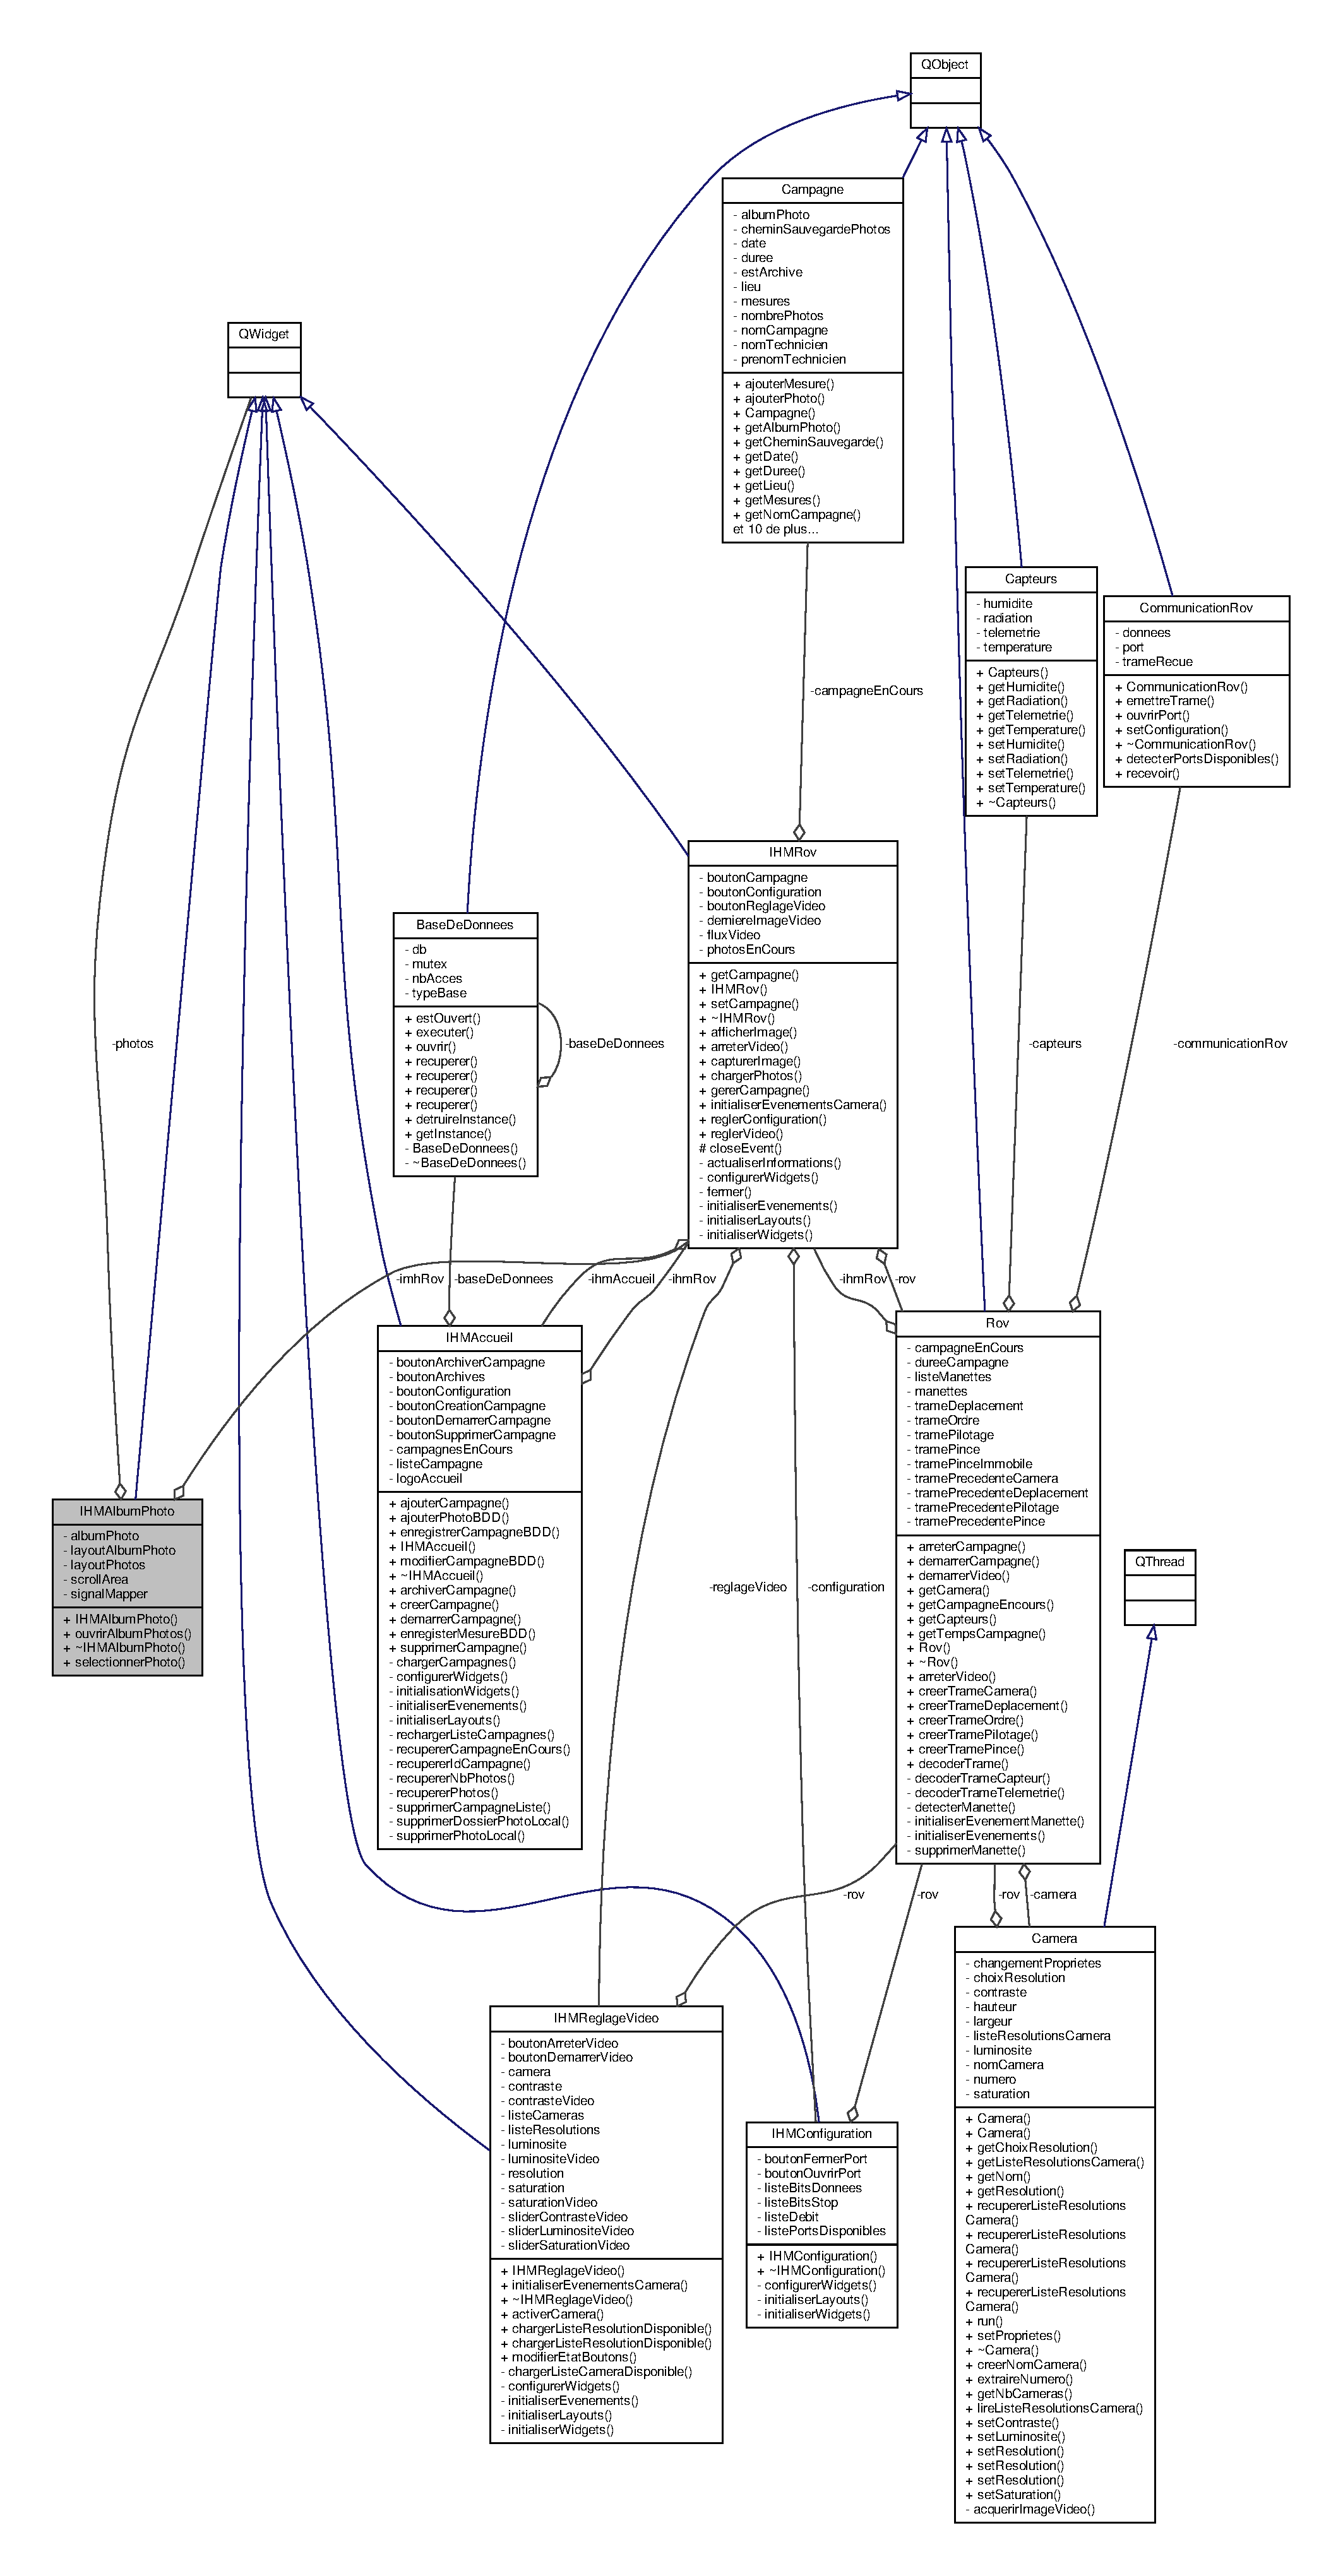
\includegraphics[height=550pt]{class_i_h_m_album_photo__coll__graph}
\end{center}
\end{figure}
\subsubsection*{Connecteurs publics}
\begin{DoxyCompactItemize}
\item 
void \hyperlink{class_i_h_m_album_photo_ad0760043151686deea04f8282e6d2210}{selectionner\+Photo} (int numero)
\begin{DoxyCompactList}\small\item\em Permet de selectionner la photo indiquer par le signal\+Mapper. \end{DoxyCompactList}\end{DoxyCompactItemize}
\subsubsection*{Fonctions membres publiques}
\begin{DoxyCompactItemize}
\item 
\hyperlink{class_i_h_m_album_photo_aefa56aaad40d6cb0ddcf769f149ab0ad}{I\+H\+M\+Album\+Photo} (\hyperlink{class_i_h_m_rov}{I\+H\+M\+Rov} $\ast$ihm\+Rov, \hyperlink{class_q_widget}{Q\+Widget} $\ast$parent=nullptr)
\begin{DoxyCompactList}\small\item\em Constructeur de la classe Album\+Photo. \end{DoxyCompactList}\item 
void \hyperlink{class_i_h_m_album_photo_a5aa9a9c1b04e00eaec1581e92649535f}{ouvrir\+Album\+Photos} (Q\+Vector$<$ \hyperlink{struct_photo}{Photo} $>$ \hyperlink{class_i_h_m_album_photo_a686adeccd626a94d9a4996782c851c61}{album\+Photo})
\begin{DoxyCompactList}\small\item\em Ouvre une nouvelle fenetre contenant la liste des photos prises en cours de mission. \end{DoxyCompactList}\item 
\hyperlink{class_i_h_m_album_photo_a02812cbcaa5467a2e6419ed9d5904cc6}{$\sim$\+I\+H\+M\+Album\+Photo} ()
\begin{DoxyCompactList}\small\item\em Destructeur de la classe Album\+Photo. \end{DoxyCompactList}\end{DoxyCompactItemize}
\subsubsection*{Attributs privés}
\begin{DoxyCompactItemize}
\item 
Q\+Vector$<$ \hyperlink{struct_photo}{Photo} $>$ \hyperlink{class_i_h_m_album_photo_a686adeccd626a94d9a4996782c851c61}{album\+Photo}
\begin{DoxyCompactList}\small\item\em Conteneur de photo. \end{DoxyCompactList}\item 
\hyperlink{class_i_h_m_rov}{I\+H\+M\+Rov} $\ast$ \hyperlink{class_i_h_m_album_photo_ab7056087d5ed3ee1528bd7f689b46c2a}{imh\+Rov}
\begin{DoxyCompactList}\small\item\em Association avec l\textquotesingle{}\hyperlink{class_i_h_m_rov}{I\+H\+M\+Rov}. \end{DoxyCompactList}\item 
Q\+V\+Box\+Layout $\ast$ \hyperlink{class_i_h_m_album_photo_a1b4028248430efc384e34b0151709fa0}{layout\+Album\+Photo}
\begin{DoxyCompactList}\small\item\em Layout s\textquotesingle{}agrandissant selon l\textquotesingle{}ajout de nouvelle photos. \end{DoxyCompactList}\item 
Q\+H\+Box\+Layout $\ast$ \hyperlink{class_i_h_m_album_photo_aabe492a016823fa63259c8e5d5b58e9d}{layout\+Photos}
\begin{DoxyCompactList}\small\item\em Layout permettant d\textquotesingle{}accueillir les différentes photos. \end{DoxyCompactList}\item 
\hyperlink{class_q_widget}{Q\+Widget} $\ast$ \hyperlink{class_i_h_m_album_photo_a0a58f758260250ac5520f2430d708d87}{photos}
\begin{DoxyCompactList}\small\item\em Emplacement permettant d\textquotesingle{}accueillir les différentes photos. \end{DoxyCompactList}\item 
Q\+Scroll\+Area $\ast$ \hyperlink{class_i_h_m_album_photo_a9ed730123be1c9ca6f7aa078ec9e0556}{scroll\+Area}
\begin{DoxyCompactList}\small\item\em Permet une defilement pour visualiser l\textquotesingle{}ensemble des photos prises durant la campagne. \end{DoxyCompactList}\item 
Q\+Signal\+Mapper $\ast$ \hyperlink{class_i_h_m_album_photo_a184d7d26edab19328980b55ce727811b}{signal\+Mapper}
\begin{DoxyCompactList}\small\item\em Objet de type Q\+Signal\+Mapper, permet d\textquotesingle{}associer chaque photo de l\textquotesingle{}\hyperlink{class_i_h_m_album_photo}{I\+H\+M\+Album\+Photo} à un signal. \end{DoxyCompactList}\end{DoxyCompactItemize}


\subsubsection{Description détaillée}
Class permettant de visualiser les photos en cours de campagne. 

Définition à la ligne \hyperlink{ihmalbumphoto_8h_source_l00035}{35} du fichier \hyperlink{ihmalbumphoto_8h_source}{ihmalbumphoto.\+h}.



\subsubsection{Documentation des constructeurs et destructeur}
\mbox{\Hypertarget{class_i_h_m_album_photo_aefa56aaad40d6cb0ddcf769f149ab0ad}\label{class_i_h_m_album_photo_aefa56aaad40d6cb0ddcf769f149ab0ad}} 
\index{I\+H\+M\+Album\+Photo@{I\+H\+M\+Album\+Photo}!I\+H\+M\+Album\+Photo@{I\+H\+M\+Album\+Photo}}
\index{I\+H\+M\+Album\+Photo@{I\+H\+M\+Album\+Photo}!I\+H\+M\+Album\+Photo@{I\+H\+M\+Album\+Photo}}
\paragraph{\texorpdfstring{I\+H\+M\+Album\+Photo()}{IHMAlbumPhoto()}}
{\footnotesize\ttfamily I\+H\+M\+Album\+Photo\+::\+I\+H\+M\+Album\+Photo (\begin{DoxyParamCaption}\item[{\hyperlink{class_i_h_m_rov}{I\+H\+M\+Rov} $\ast$}]{ihm\+Rov,  }\item[{\hyperlink{class_q_widget}{Q\+Widget} $\ast$}]{parent = {\ttfamily nullptr} }\end{DoxyParamCaption})}



Constructeur de la classe Album\+Photo. 


\begin{DoxyParams}{Paramètres}
{\em ihm\+Rov} & \\
\hline
{\em parent} & \\
\hline
\end{DoxyParams}


Définition à la ligne \hyperlink{ihmalbumphoto_8cpp_source_l00011}{11} du fichier \hyperlink{ihmalbumphoto_8cpp_source}{ihmalbumphoto.\+cpp}.



Références \hyperlink{ihmalbumphoto_8h_source_l00041}{layout\+Album\+Photo}, \hyperlink{ihmalbumphoto_8h_source_l00040}{layout\+Photos}, \hyperlink{ihmalbumphoto_8h_source_l00039}{photos}, et \hyperlink{ihmalbumphoto_8h_source_l00042}{scroll\+Area}.


\begin{DoxyCode}
00011                                                             : \hyperlink{class_q_widget}{QWidget}(parent), 
      \hyperlink{class_i_h_m_album_photo_ab7056087d5ed3ee1528bd7f689b46c2a}{imhRov}(ihmRov)
00012 \{
00013     qDebug() << Q\_FUNC\_INFO;
00014     \hyperlink{class_i_h_m_album_photo_a0a58f758260250ac5520f2430d708d87}{photos} = \textcolor{keyword}{new} \hyperlink{class_q_widget}{QWidget}();
00015     \hyperlink{class_i_h_m_album_photo_aabe492a016823fa63259c8e5d5b58e9d}{layoutPhotos} = \textcolor{keyword}{new} QHBoxLayout;
00016     \hyperlink{class_i_h_m_album_photo_a1b4028248430efc384e34b0151709fa0}{layoutAlbumPhoto} = \textcolor{keyword}{new} QVBoxLayout;
00017     \hyperlink{class_i_h_m_album_photo_a9ed730123be1c9ca6f7aa078ec9e0556}{scrollArea} = \textcolor{keyword}{new} QScrollArea();
00018 
00019     \hyperlink{class_i_h_m_album_photo_a0a58f758260250ac5520f2430d708d87}{photos}->setLayout(\hyperlink{class_i_h_m_album_photo_a1b4028248430efc384e34b0151709fa0}{layoutAlbumPhoto});
00020     \hyperlink{class_i_h_m_album_photo_a9ed730123be1c9ca6f7aa078ec9e0556}{scrollArea}->setWidgetResizable(\textcolor{keyword}{true});
00021     \hyperlink{class_i_h_m_album_photo_a9ed730123be1c9ca6f7aa078ec9e0556}{scrollArea}->setBackgroundRole(QPalette::Dark);
00022     \hyperlink{class_i_h_m_album_photo_a9ed730123be1c9ca6f7aa078ec9e0556}{scrollArea}->setFrameStyle(QFrame::Panel);
00023     \hyperlink{class_i_h_m_album_photo_a9ed730123be1c9ca6f7aa078ec9e0556}{scrollArea}->setWidget(\hyperlink{class_i_h_m_album_photo_a0a58f758260250ac5520f2430d708d87}{photos});
00024     \hyperlink{class_i_h_m_album_photo_aabe492a016823fa63259c8e5d5b58e9d}{layoutPhotos}->addWidget(\hyperlink{class_i_h_m_album_photo_a9ed730123be1c9ca6f7aa078ec9e0556}{scrollArea});
00025 
00026     setLayout(\hyperlink{class_i_h_m_album_photo_aabe492a016823fa63259c8e5d5b58e9d}{layoutPhotos});
00027 
00028     \textcolor{keywordtype}{int} width = qApp->desktop()->availableGeometry().width();
00029     \textcolor{keywordtype}{int} height = qApp->desktop()->availableGeometry().height();
00030     resize(width, height);
00031 \}
\end{DoxyCode}
\mbox{\Hypertarget{class_i_h_m_album_photo_a02812cbcaa5467a2e6419ed9d5904cc6}\label{class_i_h_m_album_photo_a02812cbcaa5467a2e6419ed9d5904cc6}} 
\index{I\+H\+M\+Album\+Photo@{I\+H\+M\+Album\+Photo}!````~I\+H\+M\+Album\+Photo@{$\sim$\+I\+H\+M\+Album\+Photo}}
\index{````~I\+H\+M\+Album\+Photo@{$\sim$\+I\+H\+M\+Album\+Photo}!I\+H\+M\+Album\+Photo@{I\+H\+M\+Album\+Photo}}
\paragraph{\texorpdfstring{$\sim$\+I\+H\+M\+Album\+Photo()}{~IHMAlbumPhoto()}}
{\footnotesize\ttfamily I\+H\+M\+Album\+Photo\+::$\sim$\+I\+H\+M\+Album\+Photo (\begin{DoxyParamCaption}{ }\end{DoxyParamCaption})}



Destructeur de la classe Album\+Photo. 



Définition à la ligne \hyperlink{ihmalbumphoto_8cpp_source_l00033}{33} du fichier \hyperlink{ihmalbumphoto_8cpp_source}{ihmalbumphoto.\+cpp}.


\begin{DoxyCode}
00034 \{
00035     qDebug() << Q\_FUNC\_INFO;
00036 \}
\end{DoxyCode}


\subsubsection{Documentation des fonctions membres}
\mbox{\Hypertarget{class_i_h_m_album_photo_a5aa9a9c1b04e00eaec1581e92649535f}\label{class_i_h_m_album_photo_a5aa9a9c1b04e00eaec1581e92649535f}} 
\index{I\+H\+M\+Album\+Photo@{I\+H\+M\+Album\+Photo}!ouvrir\+Album\+Photos@{ouvrir\+Album\+Photos}}
\index{ouvrir\+Album\+Photos@{ouvrir\+Album\+Photos}!I\+H\+M\+Album\+Photo@{I\+H\+M\+Album\+Photo}}
\paragraph{\texorpdfstring{ouvrir\+Album\+Photos()}{ouvrirAlbumPhotos()}}
{\footnotesize\ttfamily void I\+H\+M\+Album\+Photo\+::ouvrir\+Album\+Photos (\begin{DoxyParamCaption}\item[{Q\+Vector$<$ \hyperlink{struct_photo}{Photo} $>$}]{album\+Photo }\end{DoxyParamCaption})}



Ouvre une nouvelle fenetre contenant la liste des photos prises en cours de mission. 



Définition à la ligne \hyperlink{ihmalbumphoto_8cpp_source_l00038}{38} du fichier \hyperlink{ihmalbumphoto_8cpp_source}{ihmalbumphoto.\+cpp}.



Références \hyperlink{ihmalbumphoto_8h_source_l00044}{album\+Photo}, \hyperlink{ihmalbumphoto_8h_source_l00041}{layout\+Album\+Photo}, \hyperlink{ihmalbumphoto_8cpp_source_l00081}{selectionner\+Photo()}, et \hyperlink{ihmalbumphoto_8h_source_l00043}{signal\+Mapper}.



Référencé par \hyperlink{ihmrov_8cpp_source_l00223}{I\+H\+M\+Rov\+::charger\+Photos()}.


\begin{DoxyCode}
00039 \{
00040     \textcolor{keywordflow}{if}(\hyperlink{class_i_h_m_album_photo_a686adeccd626a94d9a4996782c851c61}{albumPhoto}.isEmpty())
00041     \{
00042         QMessageBox::critical(\textcolor{keyword}{this}, \textcolor{stringliteral}{"Erreur"}, \textcolor{stringliteral}{"Listes photos vide !"});
00043         \textcolor{keywordflow}{return};
00044     \}
00045 
00046     this->\hyperlink{class_i_h_m_album_photo_a686adeccd626a94d9a4996782c851c61}{albumPhoto} = \hyperlink{class_i_h_m_album_photo_a686adeccd626a94d9a4996782c851c61}{albumPhoto};
00047     \hyperlink{class_i_h_m_album_photo_a184d7d26edab19328980b55ce727811b}{signalMapper} = \textcolor{keyword}{new} QSignalMapper(\textcolor{keyword}{this});
00048     \textcolor{keywordtype}{int} numeroPhoto = 0;
00049     \textcolor{keywordflow}{for}(QVector<Photo>::iterator it = \hyperlink{class_i_h_m_album_photo_a686adeccd626a94d9a4996782c851c61}{albumPhoto}.begin(); it != 
      \hyperlink{class_i_h_m_album_photo_a686adeccd626a94d9a4996782c851c61}{albumPhoto}.end(); ++it, numeroPhoto++)
00050     \{
00051         QHBoxLayout *layoutPhoto = \textcolor{keyword}{new} QHBoxLayout;
00052         QFormLayout *layoutInformationsPhotos = \textcolor{keyword}{new} QFormLayout;
00053 
00054         QLabel *photo = \textcolor{keyword}{new} QLabel(\textcolor{keyword}{this});
00055         photo->setPixmap((*it).image);
00056 
00057         QLabel *dateHeure = \textcolor{keyword}{new} QLabel((*it).dateheure.toString(), \textcolor{keyword}{this});
00058         QLabel *chemin = \textcolor{keyword}{new} QLabel((*it).cheminSauvegarde,\textcolor{keyword}{this});
00059         QCheckBox *photoGarde = \textcolor{keyword}{new} QCheckBox(\textcolor{keyword}{this});
00060 
00061         \textcolor{keywordflow}{if}(\hyperlink{class_i_h_m_album_photo_a686adeccd626a94d9a4996782c851c61}{albumPhoto}[numeroPhoto].aGarder)
00062             photoGarde->setChecked(\textcolor{keyword}{true});
00063         \textcolor{keywordflow}{else}
00064             photoGarde->setChecked(\textcolor{keyword}{false});
00065 
00066         connect(photoGarde, SIGNAL(clicked()), \hyperlink{class_i_h_m_album_photo_a184d7d26edab19328980b55ce727811b}{signalMapper}, SLOT(map()));
00067         \hyperlink{class_i_h_m_album_photo_a184d7d26edab19328980b55ce727811b}{signalMapper}->setMapping(photoGarde, numeroPhoto);
00068 
00069         \hyperlink{class_i_h_m_album_photo_a1b4028248430efc384e34b0151709fa0}{layoutAlbumPhoto}->addLayout(layoutPhoto);
00070         layoutPhoto->addWidget(photo);
00071         layoutPhoto->addLayout(layoutInformationsPhotos);
00072         layoutInformationsPhotos->addRow(\textcolor{stringliteral}{"Date/heure : "}, dateHeure);
00073         layoutInformationsPhotos->addRow(\textcolor{stringliteral}{"Chemin photo : "}, chemin);
00074         layoutInformationsPhotos->addRow(\textcolor{stringliteral}{"Photo à archiver : "}, photoGarde);
00075     \}
00076     connect(\hyperlink{class_i_h_m_album_photo_a184d7d26edab19328980b55ce727811b}{signalMapper}, SIGNAL(mapped(\textcolor{keywordtype}{int})), \textcolor{keyword}{this}, SLOT(
      \hyperlink{class_i_h_m_album_photo_ad0760043151686deea04f8282e6d2210}{selectionnerPhoto}(\textcolor{keywordtype}{int})));
00077 
00078     this->show();
00079 \}
\end{DoxyCode}
\mbox{\Hypertarget{class_i_h_m_album_photo_ad0760043151686deea04f8282e6d2210}\label{class_i_h_m_album_photo_ad0760043151686deea04f8282e6d2210}} 
\index{I\+H\+M\+Album\+Photo@{I\+H\+M\+Album\+Photo}!selectionner\+Photo@{selectionner\+Photo}}
\index{selectionner\+Photo@{selectionner\+Photo}!I\+H\+M\+Album\+Photo@{I\+H\+M\+Album\+Photo}}
\paragraph{\texorpdfstring{selectionner\+Photo}{selectionnerPhoto}}
{\footnotesize\ttfamily void I\+H\+M\+Album\+Photo\+::selectionner\+Photo (\begin{DoxyParamCaption}\item[{int}]{numero }\end{DoxyParamCaption})\hspace{0.3cm}{\ttfamily [slot]}}



Permet de selectionner la photo indiquer par le signal\+Mapper. 


\begin{DoxyParams}{Paramètres}
{\em numero} & \\
\hline
\end{DoxyParams}


Définition à la ligne \hyperlink{ihmalbumphoto_8cpp_source_l00081}{81} du fichier \hyperlink{ihmalbumphoto_8cpp_source}{ihmalbumphoto.\+cpp}.



Références \hyperlink{ihmalbumphoto_8h_source_l00044}{album\+Photo}, \hyperlink{campagne_8cpp_source_l00070}{Campagne\+::get\+Album\+Photo()}, \hyperlink{ihmrov_8cpp_source_l00149}{I\+H\+M\+Rov\+::get\+Campagne()}, \hyperlink{ihmalbumphoto_8h_source_l00045}{imh\+Rov}, et \hyperlink{campagne_8cpp_source_l00085}{Campagne\+::modifier\+Archive\+Photo()}.



Référencé par \hyperlink{ihmalbumphoto_8cpp_source_l00038}{ouvrir\+Album\+Photos()}.


\begin{DoxyCode}
00082 \{
00083     \textcolor{keywordflow}{if}(numeroPhoto < \hyperlink{class_i_h_m_album_photo_a686adeccd626a94d9a4996782c851c61}{albumPhoto}.size())
00084     \{
00085         \hyperlink{class_i_h_m_album_photo_ab7056087d5ed3ee1528bd7f689b46c2a}{imhRov}->\hyperlink{class_i_h_m_rov_ab3e8686eef9233b4c1e6711cf1c4576a}{getCampagne}()->\hyperlink{class_campagne_a7751a5a0b5d1be46384f57b5409163e8}{modifierArchivePhoto}(numeroPhoto);
00086         qDebug() << Q\_FUNC\_INFO << \textcolor{stringliteral}{"numeroPhoto"} << numeroPhoto << \textcolor{stringliteral}{"A garder"} << 
      \hyperlink{class_i_h_m_album_photo_ab7056087d5ed3ee1528bd7f689b46c2a}{imhRov}->\hyperlink{class_i_h_m_rov_ab3e8686eef9233b4c1e6711cf1c4576a}{getCampagne}()->\hyperlink{class_campagne_abec90fcbc0c4ded45caaac9adb454add}{getAlbumPhoto}()[numeroPhoto].aGarder;
00087     \}
00088 \}
\end{DoxyCode}


\subsubsection{Documentation des données membres}
\mbox{\Hypertarget{class_i_h_m_album_photo_a686adeccd626a94d9a4996782c851c61}\label{class_i_h_m_album_photo_a686adeccd626a94d9a4996782c851c61}} 
\index{I\+H\+M\+Album\+Photo@{I\+H\+M\+Album\+Photo}!album\+Photo@{album\+Photo}}
\index{album\+Photo@{album\+Photo}!I\+H\+M\+Album\+Photo@{I\+H\+M\+Album\+Photo}}
\paragraph{\texorpdfstring{album\+Photo}{albumPhoto}}
{\footnotesize\ttfamily Q\+Vector$<$\hyperlink{struct_photo}{Photo}$>$ I\+H\+M\+Album\+Photo\+::album\+Photo\hspace{0.3cm}{\ttfamily [private]}}



Conteneur de photo. 



Définition à la ligne \hyperlink{ihmalbumphoto_8h_source_l00044}{44} du fichier \hyperlink{ihmalbumphoto_8h_source}{ihmalbumphoto.\+h}.



Référencé par \hyperlink{ihmalbumphoto_8cpp_source_l00038}{ouvrir\+Album\+Photos()}, et \hyperlink{ihmalbumphoto_8cpp_source_l00081}{selectionner\+Photo()}.

\mbox{\Hypertarget{class_i_h_m_album_photo_ab7056087d5ed3ee1528bd7f689b46c2a}\label{class_i_h_m_album_photo_ab7056087d5ed3ee1528bd7f689b46c2a}} 
\index{I\+H\+M\+Album\+Photo@{I\+H\+M\+Album\+Photo}!imh\+Rov@{imh\+Rov}}
\index{imh\+Rov@{imh\+Rov}!I\+H\+M\+Album\+Photo@{I\+H\+M\+Album\+Photo}}
\paragraph{\texorpdfstring{imh\+Rov}{imhRov}}
{\footnotesize\ttfamily \hyperlink{class_i_h_m_rov}{I\+H\+M\+Rov}$\ast$ I\+H\+M\+Album\+Photo\+::imh\+Rov\hspace{0.3cm}{\ttfamily [private]}}



Association avec l\textquotesingle{}\hyperlink{class_i_h_m_rov}{I\+H\+M\+Rov}. 



Définition à la ligne \hyperlink{ihmalbumphoto_8h_source_l00045}{45} du fichier \hyperlink{ihmalbumphoto_8h_source}{ihmalbumphoto.\+h}.



Référencé par \hyperlink{ihmalbumphoto_8cpp_source_l00081}{selectionner\+Photo()}.

\mbox{\Hypertarget{class_i_h_m_album_photo_a1b4028248430efc384e34b0151709fa0}\label{class_i_h_m_album_photo_a1b4028248430efc384e34b0151709fa0}} 
\index{I\+H\+M\+Album\+Photo@{I\+H\+M\+Album\+Photo}!layout\+Album\+Photo@{layout\+Album\+Photo}}
\index{layout\+Album\+Photo@{layout\+Album\+Photo}!I\+H\+M\+Album\+Photo@{I\+H\+M\+Album\+Photo}}
\paragraph{\texorpdfstring{layout\+Album\+Photo}{layoutAlbumPhoto}}
{\footnotesize\ttfamily Q\+V\+Box\+Layout$\ast$ I\+H\+M\+Album\+Photo\+::layout\+Album\+Photo\hspace{0.3cm}{\ttfamily [private]}}



Layout s\textquotesingle{}agrandissant selon l\textquotesingle{}ajout de nouvelle photos. 



Définition à la ligne \hyperlink{ihmalbumphoto_8h_source_l00041}{41} du fichier \hyperlink{ihmalbumphoto_8h_source}{ihmalbumphoto.\+h}.



Référencé par \hyperlink{ihmalbumphoto_8cpp_source_l00011}{I\+H\+M\+Album\+Photo()}, et \hyperlink{ihmalbumphoto_8cpp_source_l00038}{ouvrir\+Album\+Photos()}.

\mbox{\Hypertarget{class_i_h_m_album_photo_aabe492a016823fa63259c8e5d5b58e9d}\label{class_i_h_m_album_photo_aabe492a016823fa63259c8e5d5b58e9d}} 
\index{I\+H\+M\+Album\+Photo@{I\+H\+M\+Album\+Photo}!layout\+Photos@{layout\+Photos}}
\index{layout\+Photos@{layout\+Photos}!I\+H\+M\+Album\+Photo@{I\+H\+M\+Album\+Photo}}
\paragraph{\texorpdfstring{layout\+Photos}{layoutPhotos}}
{\footnotesize\ttfamily Q\+H\+Box\+Layout$\ast$ I\+H\+M\+Album\+Photo\+::layout\+Photos\hspace{0.3cm}{\ttfamily [private]}}



Layout permettant d\textquotesingle{}accueillir les différentes photos. 



Définition à la ligne \hyperlink{ihmalbumphoto_8h_source_l00040}{40} du fichier \hyperlink{ihmalbumphoto_8h_source}{ihmalbumphoto.\+h}.



Référencé par \hyperlink{ihmalbumphoto_8cpp_source_l00011}{I\+H\+M\+Album\+Photo()}.

\mbox{\Hypertarget{class_i_h_m_album_photo_a0a58f758260250ac5520f2430d708d87}\label{class_i_h_m_album_photo_a0a58f758260250ac5520f2430d708d87}} 
\index{I\+H\+M\+Album\+Photo@{I\+H\+M\+Album\+Photo}!photos@{photos}}
\index{photos@{photos}!I\+H\+M\+Album\+Photo@{I\+H\+M\+Album\+Photo}}
\paragraph{\texorpdfstring{photos}{photos}}
{\footnotesize\ttfamily \hyperlink{class_q_widget}{Q\+Widget}$\ast$ I\+H\+M\+Album\+Photo\+::photos\hspace{0.3cm}{\ttfamily [private]}}



Emplacement permettant d\textquotesingle{}accueillir les différentes photos. 



Définition à la ligne \hyperlink{ihmalbumphoto_8h_source_l00039}{39} du fichier \hyperlink{ihmalbumphoto_8h_source}{ihmalbumphoto.\+h}.



Référencé par \hyperlink{ihmalbumphoto_8cpp_source_l00011}{I\+H\+M\+Album\+Photo()}.

\mbox{\Hypertarget{class_i_h_m_album_photo_a9ed730123be1c9ca6f7aa078ec9e0556}\label{class_i_h_m_album_photo_a9ed730123be1c9ca6f7aa078ec9e0556}} 
\index{I\+H\+M\+Album\+Photo@{I\+H\+M\+Album\+Photo}!scroll\+Area@{scroll\+Area}}
\index{scroll\+Area@{scroll\+Area}!I\+H\+M\+Album\+Photo@{I\+H\+M\+Album\+Photo}}
\paragraph{\texorpdfstring{scroll\+Area}{scrollArea}}
{\footnotesize\ttfamily Q\+Scroll\+Area$\ast$ I\+H\+M\+Album\+Photo\+::scroll\+Area\hspace{0.3cm}{\ttfamily [private]}}



Permet une defilement pour visualiser l\textquotesingle{}ensemble des photos prises durant la campagne. 



Définition à la ligne \hyperlink{ihmalbumphoto_8h_source_l00042}{42} du fichier \hyperlink{ihmalbumphoto_8h_source}{ihmalbumphoto.\+h}.



Référencé par \hyperlink{ihmalbumphoto_8cpp_source_l00011}{I\+H\+M\+Album\+Photo()}.

\mbox{\Hypertarget{class_i_h_m_album_photo_a184d7d26edab19328980b55ce727811b}\label{class_i_h_m_album_photo_a184d7d26edab19328980b55ce727811b}} 
\index{I\+H\+M\+Album\+Photo@{I\+H\+M\+Album\+Photo}!signal\+Mapper@{signal\+Mapper}}
\index{signal\+Mapper@{signal\+Mapper}!I\+H\+M\+Album\+Photo@{I\+H\+M\+Album\+Photo}}
\paragraph{\texorpdfstring{signal\+Mapper}{signalMapper}}
{\footnotesize\ttfamily Q\+Signal\+Mapper$\ast$ I\+H\+M\+Album\+Photo\+::signal\+Mapper\hspace{0.3cm}{\ttfamily [private]}}



Objet de type Q\+Signal\+Mapper, permet d\textquotesingle{}associer chaque photo de l\textquotesingle{}\hyperlink{class_i_h_m_album_photo}{I\+H\+M\+Album\+Photo} à un signal. 



Définition à la ligne \hyperlink{ihmalbumphoto_8h_source_l00043}{43} du fichier \hyperlink{ihmalbumphoto_8h_source}{ihmalbumphoto.\+h}.



Référencé par \hyperlink{ihmalbumphoto_8cpp_source_l00038}{ouvrir\+Album\+Photos()}.



La documentation de cette classe a été générée à partir des fichiers suivants \+:\begin{DoxyCompactItemize}
\item 
\hyperlink{ihmalbumphoto_8h}{ihmalbumphoto.\+h}\item 
\hyperlink{ihmalbumphoto_8cpp}{ihmalbumphoto.\+cpp}\end{DoxyCompactItemize}

\hypertarget{class_i_h_m_configuration}{}\subsection{Référence de la classe I\+H\+M\+Configuration}
\label{class_i_h_m_configuration}\index{I\+H\+M\+Configuration@{I\+H\+M\+Configuration}}


Class permettant de configurer la communication avec le rov.  




{\ttfamily \#include \char`\"{}ihmconfiguration.\+h\char`\"{}}



Graphe de collaboration de I\+H\+M\+Configuration\+:
\nopagebreak
\begin{figure}[H]
\begin{center}
\leavevmode
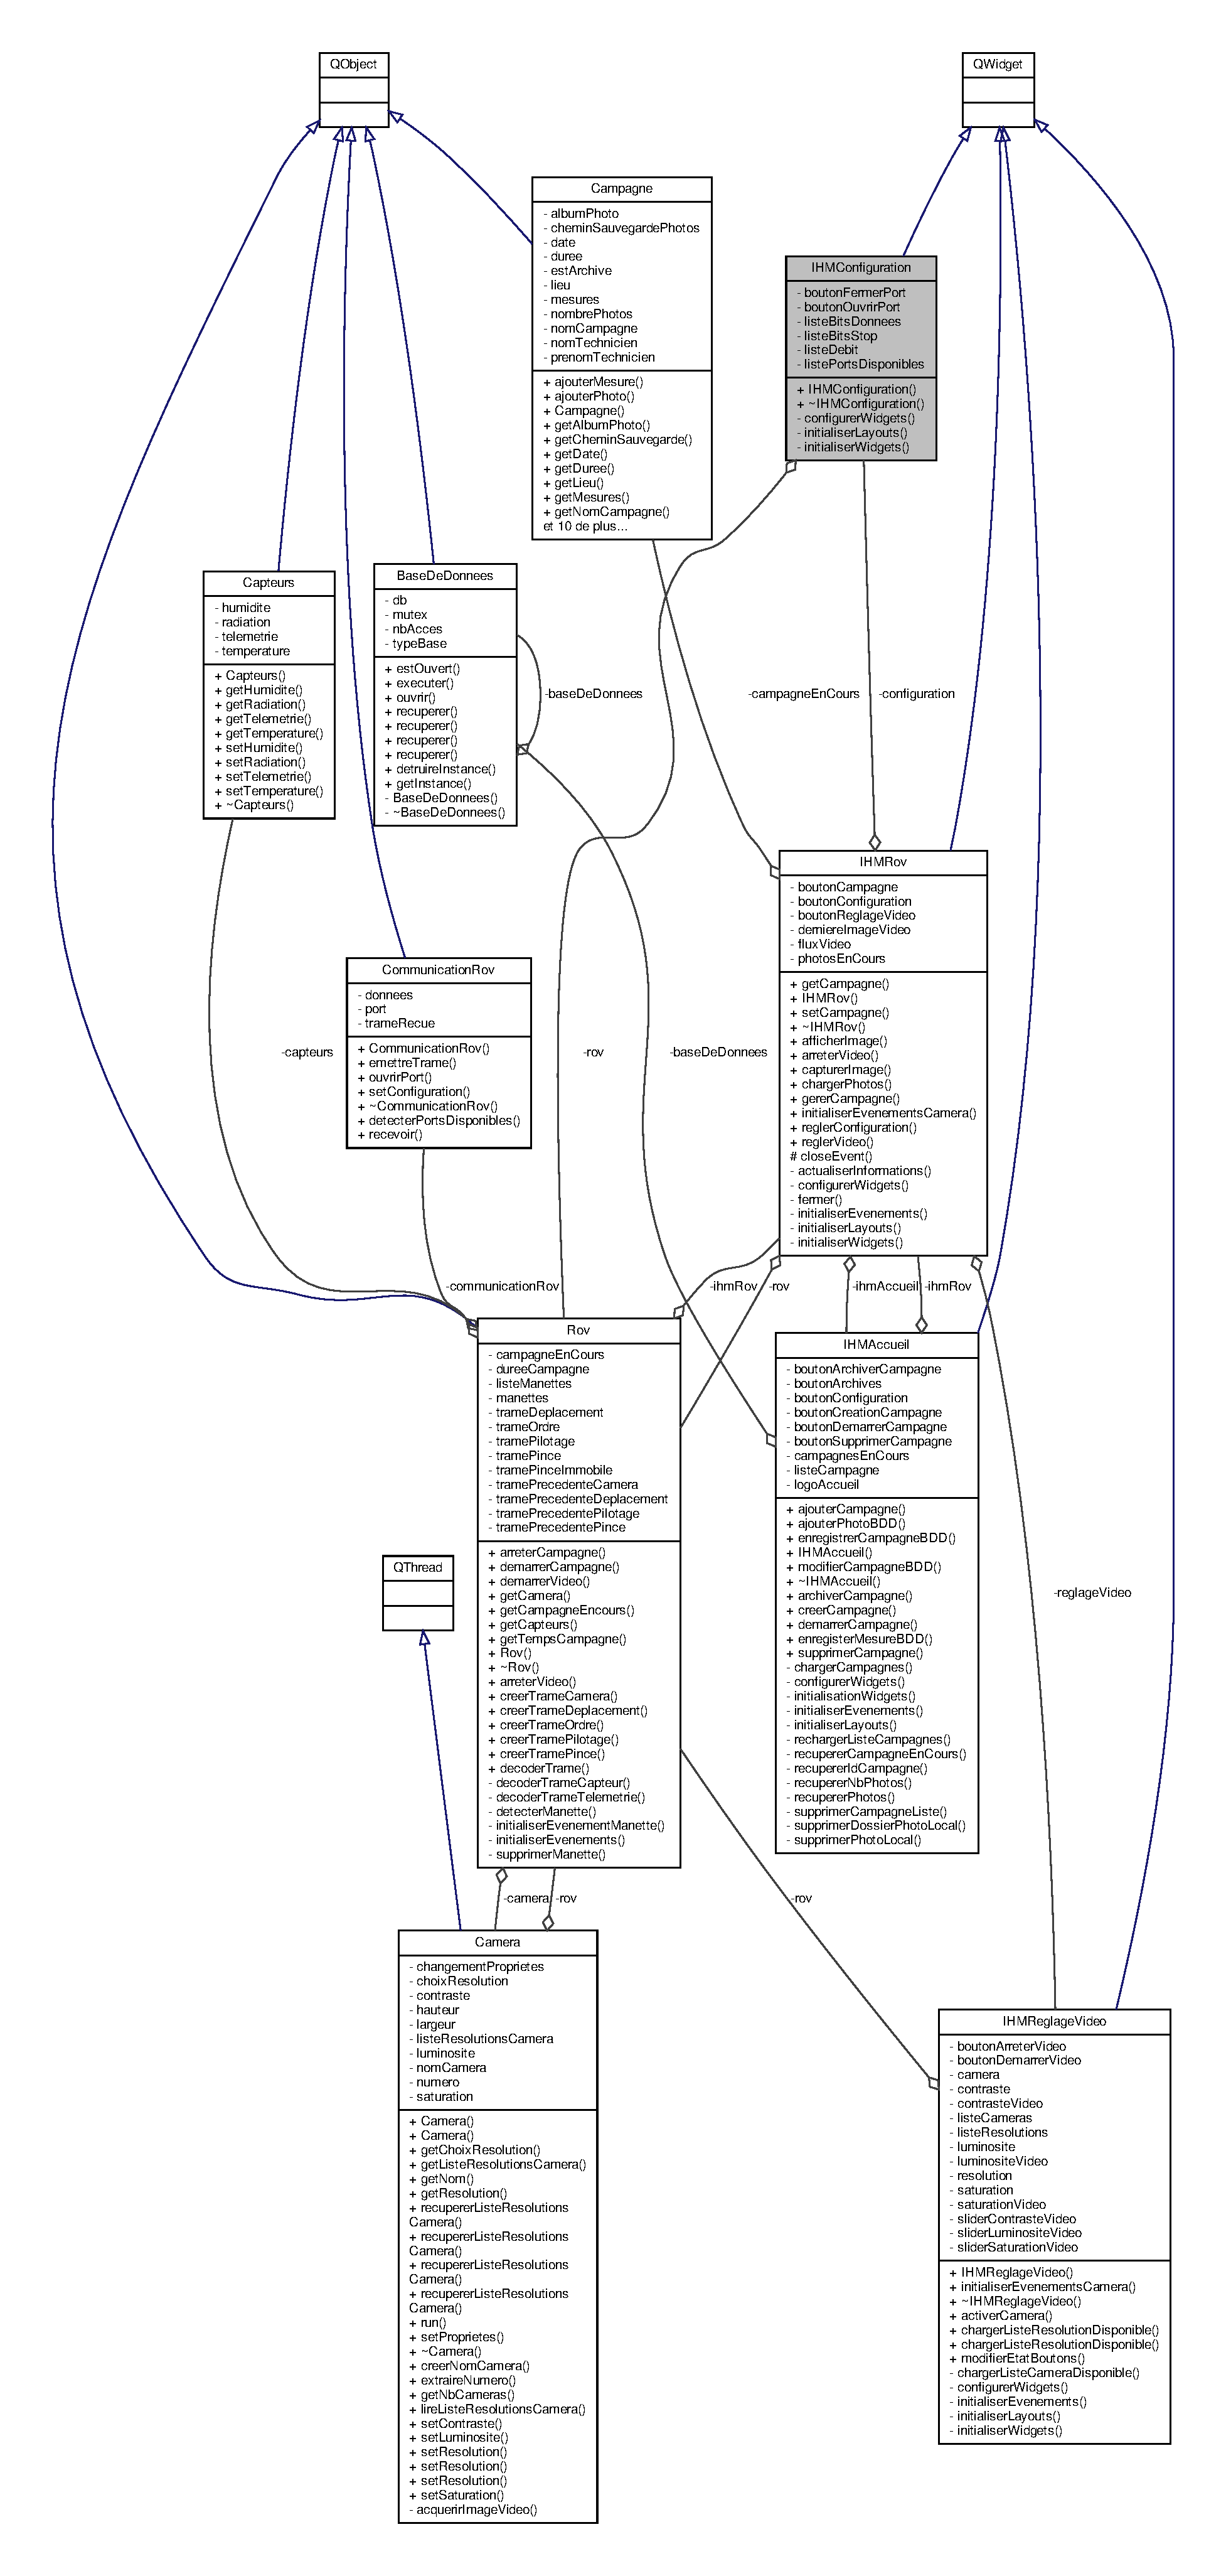
\includegraphics[height=550pt]{class_i_h_m_configuration__coll__graph}
\end{center}
\end{figure}
\subsubsection*{Fonctions membres publiques}
\begin{DoxyCompactItemize}
\item 
\hyperlink{class_i_h_m_configuration_a1532c281d170546071352cfe05feb1b8}{I\+H\+M\+Configuration} (\hyperlink{class_rov}{Rov} $\ast$\hyperlink{class_i_h_m_configuration_a75a7e5b7312d9eb3377bc96372fc0b3a}{rov}, \hyperlink{class_q_widget}{Q\+Widget} $\ast$parent=nullptr)
\begin{DoxyCompactList}\small\item\em Constructeur de la classe \hyperlink{class_i_h_m_configuration}{I\+H\+M\+Configuration}. \end{DoxyCompactList}\item 
\hyperlink{class_i_h_m_configuration_a59e2b693b4a1f1a8a6af3227996c3808}{$\sim$\+I\+H\+M\+Configuration} ()
\begin{DoxyCompactList}\small\item\em Destructeur de la classe \hyperlink{class_i_h_m_configuration}{I\+H\+M\+Configuration}. \end{DoxyCompactList}\end{DoxyCompactItemize}
\subsubsection*{Fonctions membres privées}
\begin{DoxyCompactItemize}
\item 
void \hyperlink{class_i_h_m_configuration_a9ed73ca9584b8d9f33ad341081113a55}{configurer\+Widgets} ()
\begin{DoxyCompactList}\small\item\em Configure l\textquotesingle{}état des widgets à la création de l\textquotesingle{}I\+HM. \end{DoxyCompactList}\item 
void \hyperlink{class_i_h_m_configuration_ab76abe78fff3b7945b675acddbd320f0}{initialiser\+Layouts} ()
\begin{DoxyCompactList}\small\item\em Initialise les layouts de l\textquotesingle{}I\+HM. \end{DoxyCompactList}\item 
void \hyperlink{class_i_h_m_configuration_a76fe56bbd88aef5581186e05fb4ae67f}{initialiser\+Widgets} ()
\begin{DoxyCompactList}\small\item\em Initialise les widgets de l\textquotesingle{}I\+HM. \end{DoxyCompactList}\end{DoxyCompactItemize}
\subsubsection*{Attributs privés}
\begin{DoxyCompactItemize}
\item 
Q\+Push\+Button $\ast$ \hyperlink{class_i_h_m_configuration_a25c0b3c51a8d162ae3439a56ec644909}{bouton\+Fermer\+Port}
\begin{DoxyCompactList}\small\item\em Bouton permettant de fermer le port sélectionné \end{DoxyCompactList}\item 
Q\+Push\+Button $\ast$ \hyperlink{class_i_h_m_configuration_a824b7f6c0d332b8f6f76801e545b14ad}{bouton\+Ouvrir\+Port}
\begin{DoxyCompactList}\small\item\em Bouton permettant d\textquotesingle{}ouvrir le port sélectionné \end{DoxyCompactList}\item 
Q\+Combo\+Box $\ast$ \hyperlink{class_i_h_m_configuration_a83c61d075d53758bd753aada9a0bb452}{liste\+Bits\+Donnees}
\begin{DoxyCompactList}\small\item\em Liste permettant de configurer le nombre de bits de données de la communication. \end{DoxyCompactList}\item 
Q\+Combo\+Box $\ast$ \hyperlink{class_i_h_m_configuration_a16ae724388b797983c78e87e7d5485cb}{liste\+Bits\+Stop}
\begin{DoxyCompactList}\small\item\em Liste permettant de configurer le nombre de bits de stop de la communication. \end{DoxyCompactList}\item 
Q\+Combo\+Box $\ast$ \hyperlink{class_i_h_m_configuration_a98e8133a04509b3a80b232d2f031e81f}{liste\+Debit}
\begin{DoxyCompactList}\small\item\em Liste permettant de configurer le debit de la communication. \end{DoxyCompactList}\item 
Q\+Combo\+Box $\ast$ \hyperlink{class_i_h_m_configuration_af3ce74444e24237aedf1d2ef2053b574}{liste\+Ports\+Disponibles}
\begin{DoxyCompactList}\small\item\em Liste des ports détéctés. \end{DoxyCompactList}\item 
\hyperlink{class_rov}{Rov} $\ast$ \hyperlink{class_i_h_m_configuration_a75a7e5b7312d9eb3377bc96372fc0b3a}{rov}
\begin{DoxyCompactList}\small\item\em Objet rov permettant de mofidier les reglage de la communication. \end{DoxyCompactList}\end{DoxyCompactItemize}


\subsubsection{Description détaillée}
Class permettant de configurer la communication avec le rov. 

Définition à la ligne \hyperlink{ihmconfiguration_8h_source_l00020}{20} du fichier \hyperlink{ihmconfiguration_8h_source}{ihmconfiguration.\+h}.



\subsubsection{Documentation des constructeurs et destructeur}
\mbox{\Hypertarget{class_i_h_m_configuration_a1532c281d170546071352cfe05feb1b8}\label{class_i_h_m_configuration_a1532c281d170546071352cfe05feb1b8}} 
\index{I\+H\+M\+Configuration@{I\+H\+M\+Configuration}!I\+H\+M\+Configuration@{I\+H\+M\+Configuration}}
\index{I\+H\+M\+Configuration@{I\+H\+M\+Configuration}!I\+H\+M\+Configuration@{I\+H\+M\+Configuration}}
\paragraph{\texorpdfstring{I\+H\+M\+Configuration()}{IHMConfiguration()}}
{\footnotesize\ttfamily I\+H\+M\+Configuration\+::\+I\+H\+M\+Configuration (\begin{DoxyParamCaption}\item[{\hyperlink{class_rov}{Rov} $\ast$}]{rov,  }\item[{\hyperlink{class_q_widget}{Q\+Widget} $\ast$}]{parent = {\ttfamily nullptr} }\end{DoxyParamCaption})}



Constructeur de la classe \hyperlink{class_i_h_m_configuration}{I\+H\+M\+Configuration}. 


\begin{DoxyParams}{Paramètres}
{\em rov} & \\
\hline
{\em parent} & \\
\hline
\end{DoxyParams}


Définition à la ligne \hyperlink{ihmconfiguration_8cpp_source_l00009}{9} du fichier \hyperlink{ihmconfiguration_8cpp_source}{ihmconfiguration.\+cpp}.



Références \hyperlink{ihmconfiguration_8cpp_source_l00033}{configurer\+Widgets()}, \hyperlink{ihmconfiguration_8cpp_source_l00051}{initialiser\+Layouts()}, et \hyperlink{ihmconfiguration_8cpp_source_l00023}{initialiser\+Widgets()}.


\begin{DoxyCode}
00009                                                             : \hyperlink{class_q_widget}{QWidget}(parent), 
      \hyperlink{class_i_h_m_configuration_a75a7e5b7312d9eb3377bc96372fc0b3a}{rov}(rov)
00010 \{
00011     qDebug() << Q\_FUNC\_INFO;
00012 
00013     \hyperlink{class_i_h_m_configuration_a76fe56bbd88aef5581186e05fb4ae67f}{initialiserWidgets}();
00014     \hyperlink{class_i_h_m_configuration_a9ed73ca9584b8d9f33ad341081113a55}{configurerWidgets}();
00015     \hyperlink{class_i_h_m_configuration_ab76abe78fff3b7945b675acddbd320f0}{initialiserLayouts}();
00016 \}
\end{DoxyCode}
\mbox{\Hypertarget{class_i_h_m_configuration_a59e2b693b4a1f1a8a6af3227996c3808}\label{class_i_h_m_configuration_a59e2b693b4a1f1a8a6af3227996c3808}} 
\index{I\+H\+M\+Configuration@{I\+H\+M\+Configuration}!````~I\+H\+M\+Configuration@{$\sim$\+I\+H\+M\+Configuration}}
\index{````~I\+H\+M\+Configuration@{$\sim$\+I\+H\+M\+Configuration}!I\+H\+M\+Configuration@{I\+H\+M\+Configuration}}
\paragraph{\texorpdfstring{$\sim$\+I\+H\+M\+Configuration()}{~IHMConfiguration()}}
{\footnotesize\ttfamily I\+H\+M\+Configuration\+::$\sim$\+I\+H\+M\+Configuration (\begin{DoxyParamCaption}{ }\end{DoxyParamCaption})}



Destructeur de la classe \hyperlink{class_i_h_m_configuration}{I\+H\+M\+Configuration}. 



Définition à la ligne \hyperlink{ihmconfiguration_8cpp_source_l00018}{18} du fichier \hyperlink{ihmconfiguration_8cpp_source}{ihmconfiguration.\+cpp}.


\begin{DoxyCode}
00019 \{
00020     qDebug() << Q\_FUNC\_INFO;
00021 \}
\end{DoxyCode}


\subsubsection{Documentation des fonctions membres}
\mbox{\Hypertarget{class_i_h_m_configuration_a9ed73ca9584b8d9f33ad341081113a55}\label{class_i_h_m_configuration_a9ed73ca9584b8d9f33ad341081113a55}} 
\index{I\+H\+M\+Configuration@{I\+H\+M\+Configuration}!configurer\+Widgets@{configurer\+Widgets}}
\index{configurer\+Widgets@{configurer\+Widgets}!I\+H\+M\+Configuration@{I\+H\+M\+Configuration}}
\paragraph{\texorpdfstring{configurer\+Widgets()}{configurerWidgets()}}
{\footnotesize\ttfamily void I\+H\+M\+Configuration\+::configurer\+Widgets (\begin{DoxyParamCaption}{ }\end{DoxyParamCaption})\hspace{0.3cm}{\ttfamily [private]}}



Configure l\textquotesingle{}état des widgets à la création de l\textquotesingle{}I\+HM. 



Définition à la ligne \hyperlink{ihmconfiguration_8cpp_source_l00033}{33} du fichier \hyperlink{ihmconfiguration_8cpp_source}{ihmconfiguration.\+cpp}.



Références \hyperlink{ihmconfiguration_8h_source_l00030}{bouton\+Fermer\+Port}, \hyperlink{communicationrov_8cpp_source_l00090}{Communication\+Rov\+::detecter\+Ports\+Disponibles()}, \hyperlink{ihmconfiguration_8h_source_l00027}{liste\+Bits\+Donnees}, \hyperlink{ihmconfiguration_8h_source_l00028}{liste\+Bits\+Stop}, \hyperlink{ihmconfiguration_8h_source_l00026}{liste\+Debit}, et \hyperlink{ihmconfiguration_8h_source_l00025}{liste\+Ports\+Disponibles}.



Référencé par \hyperlink{ihmconfiguration_8cpp_source_l00009}{I\+H\+M\+Configuration()}.


\begin{DoxyCode}
00034 \{
00035     \hyperlink{class_i_h_m_configuration_af3ce74444e24237aedf1d2ef2053b574}{listePortsDisponibles}->addItems(
      \hyperlink{class_communication_rov_ad9882c08083c66cd89b472b9244727e9}{CommunicationRov::detecterPortsDisponibles}());
00036     \textcolor{keywordflow}{if}(\hyperlink{class_i_h_m_configuration_af3ce74444e24237aedf1d2ef2053b574}{listePortsDisponibles}->currentText() == \textcolor{stringliteral}{""})
00037         \hyperlink{class_i_h_m_configuration_af3ce74444e24237aedf1d2ef2053b574}{listePortsDisponibles}->addItem(\textcolor{stringliteral}{"Aucun ports détécté"});
00038     \hyperlink{class_i_h_m_configuration_a98e8133a04509b3a80b232d2f031e81f}{listeDebit}->addItem(\textcolor{stringliteral}{"9600"});
00039     \hyperlink{class_i_h_m_configuration_a98e8133a04509b3a80b232d2f031e81f}{listeDebit}->addItem(\textcolor{stringliteral}{"115200"});
00040 
00041     \hyperlink{class_i_h_m_configuration_a83c61d075d53758bd753aada9a0bb452}{listeBitsDonnees}->addItem(\textcolor{stringliteral}{"7"});
00042     \hyperlink{class_i_h_m_configuration_a83c61d075d53758bd753aada9a0bb452}{listeBitsDonnees}->addItem(\textcolor{stringliteral}{"8"});
00043     \hyperlink{class_i_h_m_configuration_a83c61d075d53758bd753aada9a0bb452}{listeBitsDonnees}->setCurrentIndex(1);
00044 
00045     \hyperlink{class_i_h_m_configuration_a16ae724388b797983c78e87e7d5485cb}{listeBitsStop}->addItem(\textcolor{stringliteral}{"1"});
00046     \hyperlink{class_i_h_m_configuration_a16ae724388b797983c78e87e7d5485cb}{listeBitsStop}->addItem(\textcolor{stringliteral}{"2"});
00047 
00048     \hyperlink{class_i_h_m_configuration_a25c0b3c51a8d162ae3439a56ec644909}{boutonFermerPort}->setDisabled(\textcolor{keyword}{true});
00049 \}
\end{DoxyCode}
\mbox{\Hypertarget{class_i_h_m_configuration_ab76abe78fff3b7945b675acddbd320f0}\label{class_i_h_m_configuration_ab76abe78fff3b7945b675acddbd320f0}} 
\index{I\+H\+M\+Configuration@{I\+H\+M\+Configuration}!initialiser\+Layouts@{initialiser\+Layouts}}
\index{initialiser\+Layouts@{initialiser\+Layouts}!I\+H\+M\+Configuration@{I\+H\+M\+Configuration}}
\paragraph{\texorpdfstring{initialiser\+Layouts()}{initialiserLayouts()}}
{\footnotesize\ttfamily void I\+H\+M\+Configuration\+::initialiser\+Layouts (\begin{DoxyParamCaption}{ }\end{DoxyParamCaption})\hspace{0.3cm}{\ttfamily [private]}}



Initialise les layouts de l\textquotesingle{}I\+HM. 



Définition à la ligne \hyperlink{ihmconfiguration_8cpp_source_l00051}{51} du fichier \hyperlink{ihmconfiguration_8cpp_source}{ihmconfiguration.\+cpp}.



Références \hyperlink{ihmconfiguration_8h_source_l00030}{bouton\+Fermer\+Port}, \hyperlink{ihmconfiguration_8h_source_l00029}{bouton\+Ouvrir\+Port}, \hyperlink{ihmconfiguration_8h_source_l00027}{liste\+Bits\+Donnees}, \hyperlink{ihmconfiguration_8h_source_l00028}{liste\+Bits\+Stop}, \hyperlink{ihmconfiguration_8h_source_l00026}{liste\+Debit}, et \hyperlink{ihmconfiguration_8h_source_l00025}{liste\+Ports\+Disponibles}.



Référencé par \hyperlink{ihmconfiguration_8cpp_source_l00009}{I\+H\+M\+Configuration()}.


\begin{DoxyCode}
00052 \{
00053     QVBoxLayout *layoutPrincipal = \textcolor{keyword}{new} QVBoxLayout;
00054     QHBoxLayout *layoutInformation = \textcolor{keyword}{new} QHBoxLayout;
00055     QFormLayout *layoutConfiguration = \textcolor{keyword}{new} QFormLayout;
00056     QVBoxLayout *layoutCommande = \textcolor{keyword}{new} QVBoxLayout;
00057 
00058     layoutCommande->setAlignment(Qt::AlignTop);
00059 
00060     layoutPrincipal->addLayout(layoutInformation);
00061     layoutInformation->addLayout(layoutConfiguration);
00062     layoutInformation->addLayout(layoutCommande);
00063     layoutConfiguration->addRow(\textcolor{stringliteral}{"Port:"}, \hyperlink{class_i_h_m_configuration_af3ce74444e24237aedf1d2ef2053b574}{listePortsDisponibles});
00064     layoutConfiguration->addRow(\textcolor{stringliteral}{"Débit:"}, \hyperlink{class_i_h_m_configuration_a98e8133a04509b3a80b232d2f031e81f}{listeDebit});
00065     layoutConfiguration->addRow(\textcolor{stringliteral}{"Bits de données:"}, \hyperlink{class_i_h_m_configuration_a83c61d075d53758bd753aada9a0bb452}{listeBitsDonnees});
00066     layoutConfiguration->addRow(\textcolor{stringliteral}{"Bits de stop:"}, \hyperlink{class_i_h_m_configuration_a16ae724388b797983c78e87e7d5485cb}{listeBitsStop});
00067     layoutCommande->addWidget(\hyperlink{class_i_h_m_configuration_a824b7f6c0d332b8f6f76801e545b14ad}{boutonOuvrirPort});
00068     layoutCommande->addWidget(\hyperlink{class_i_h_m_configuration_a25c0b3c51a8d162ae3439a56ec644909}{boutonFermerPort});
00069 
00070     setLayout(layoutPrincipal);
00071 \}
\end{DoxyCode}
\mbox{\Hypertarget{class_i_h_m_configuration_a76fe56bbd88aef5581186e05fb4ae67f}\label{class_i_h_m_configuration_a76fe56bbd88aef5581186e05fb4ae67f}} 
\index{I\+H\+M\+Configuration@{I\+H\+M\+Configuration}!initialiser\+Widgets@{initialiser\+Widgets}}
\index{initialiser\+Widgets@{initialiser\+Widgets}!I\+H\+M\+Configuration@{I\+H\+M\+Configuration}}
\paragraph{\texorpdfstring{initialiser\+Widgets()}{initialiserWidgets()}}
{\footnotesize\ttfamily void I\+H\+M\+Configuration\+::initialiser\+Widgets (\begin{DoxyParamCaption}{ }\end{DoxyParamCaption})\hspace{0.3cm}{\ttfamily [private]}}



Initialise les widgets de l\textquotesingle{}I\+HM. 



Définition à la ligne \hyperlink{ihmconfiguration_8cpp_source_l00023}{23} du fichier \hyperlink{ihmconfiguration_8cpp_source}{ihmconfiguration.\+cpp}.



Références \hyperlink{ihmconfiguration_8h_source_l00030}{bouton\+Fermer\+Port}, \hyperlink{ihmconfiguration_8h_source_l00029}{bouton\+Ouvrir\+Port}, \hyperlink{ihmconfiguration_8h_source_l00027}{liste\+Bits\+Donnees}, \hyperlink{ihmconfiguration_8h_source_l00028}{liste\+Bits\+Stop}, \hyperlink{ihmconfiguration_8h_source_l00026}{liste\+Debit}, et \hyperlink{ihmconfiguration_8h_source_l00025}{liste\+Ports\+Disponibles}.



Référencé par \hyperlink{ihmconfiguration_8cpp_source_l00009}{I\+H\+M\+Configuration()}.


\begin{DoxyCode}
00024 \{
00025     \hyperlink{class_i_h_m_configuration_af3ce74444e24237aedf1d2ef2053b574}{listePortsDisponibles} = \textcolor{keyword}{new} QComboBox(\textcolor{keyword}{this});
00026     \hyperlink{class_i_h_m_configuration_a98e8133a04509b3a80b232d2f031e81f}{listeDebit} = \textcolor{keyword}{new} QComboBox(\textcolor{keyword}{this});
00027     \hyperlink{class_i_h_m_configuration_a83c61d075d53758bd753aada9a0bb452}{listeBitsDonnees} = \textcolor{keyword}{new} QComboBox(\textcolor{keyword}{this});
00028     \hyperlink{class_i_h_m_configuration_a16ae724388b797983c78e87e7d5485cb}{listeBitsStop} = \textcolor{keyword}{new} QComboBox(\textcolor{keyword}{this});
00029     \hyperlink{class_i_h_m_configuration_a824b7f6c0d332b8f6f76801e545b14ad}{boutonOuvrirPort} = \textcolor{keyword}{new} QPushButton(\textcolor{stringliteral}{"Ouvrir"}, \textcolor{keyword}{this});
00030     \hyperlink{class_i_h_m_configuration_a25c0b3c51a8d162ae3439a56ec644909}{boutonFermerPort} = \textcolor{keyword}{new} QPushButton(\textcolor{stringliteral}{"Fermer"}, \textcolor{keyword}{this});
00031 \}
\end{DoxyCode}


\subsubsection{Documentation des données membres}
\mbox{\Hypertarget{class_i_h_m_configuration_a25c0b3c51a8d162ae3439a56ec644909}\label{class_i_h_m_configuration_a25c0b3c51a8d162ae3439a56ec644909}} 
\index{I\+H\+M\+Configuration@{I\+H\+M\+Configuration}!bouton\+Fermer\+Port@{bouton\+Fermer\+Port}}
\index{bouton\+Fermer\+Port@{bouton\+Fermer\+Port}!I\+H\+M\+Configuration@{I\+H\+M\+Configuration}}
\paragraph{\texorpdfstring{bouton\+Fermer\+Port}{boutonFermerPort}}
{\footnotesize\ttfamily Q\+Push\+Button$\ast$ I\+H\+M\+Configuration\+::bouton\+Fermer\+Port\hspace{0.3cm}{\ttfamily [private]}}



Bouton permettant de fermer le port sélectionné 



Définition à la ligne \hyperlink{ihmconfiguration_8h_source_l00030}{30} du fichier \hyperlink{ihmconfiguration_8h_source}{ihmconfiguration.\+h}.



Référencé par \hyperlink{ihmconfiguration_8cpp_source_l00033}{configurer\+Widgets()}, \hyperlink{ihmconfiguration_8cpp_source_l00051}{initialiser\+Layouts()}, et \hyperlink{ihmconfiguration_8cpp_source_l00023}{initialiser\+Widgets()}.

\mbox{\Hypertarget{class_i_h_m_configuration_a824b7f6c0d332b8f6f76801e545b14ad}\label{class_i_h_m_configuration_a824b7f6c0d332b8f6f76801e545b14ad}} 
\index{I\+H\+M\+Configuration@{I\+H\+M\+Configuration}!bouton\+Ouvrir\+Port@{bouton\+Ouvrir\+Port}}
\index{bouton\+Ouvrir\+Port@{bouton\+Ouvrir\+Port}!I\+H\+M\+Configuration@{I\+H\+M\+Configuration}}
\paragraph{\texorpdfstring{bouton\+Ouvrir\+Port}{boutonOuvrirPort}}
{\footnotesize\ttfamily Q\+Push\+Button$\ast$ I\+H\+M\+Configuration\+::bouton\+Ouvrir\+Port\hspace{0.3cm}{\ttfamily [private]}}



Bouton permettant d\textquotesingle{}ouvrir le port sélectionné 



Définition à la ligne \hyperlink{ihmconfiguration_8h_source_l00029}{29} du fichier \hyperlink{ihmconfiguration_8h_source}{ihmconfiguration.\+h}.



Référencé par \hyperlink{ihmconfiguration_8cpp_source_l00051}{initialiser\+Layouts()}, et \hyperlink{ihmconfiguration_8cpp_source_l00023}{initialiser\+Widgets()}.

\mbox{\Hypertarget{class_i_h_m_configuration_a83c61d075d53758bd753aada9a0bb452}\label{class_i_h_m_configuration_a83c61d075d53758bd753aada9a0bb452}} 
\index{I\+H\+M\+Configuration@{I\+H\+M\+Configuration}!liste\+Bits\+Donnees@{liste\+Bits\+Donnees}}
\index{liste\+Bits\+Donnees@{liste\+Bits\+Donnees}!I\+H\+M\+Configuration@{I\+H\+M\+Configuration}}
\paragraph{\texorpdfstring{liste\+Bits\+Donnees}{listeBitsDonnees}}
{\footnotesize\ttfamily Q\+Combo\+Box$\ast$ I\+H\+M\+Configuration\+::liste\+Bits\+Donnees\hspace{0.3cm}{\ttfamily [private]}}



Liste permettant de configurer le nombre de bits de données de la communication. 



Définition à la ligne \hyperlink{ihmconfiguration_8h_source_l00027}{27} du fichier \hyperlink{ihmconfiguration_8h_source}{ihmconfiguration.\+h}.



Référencé par \hyperlink{ihmconfiguration_8cpp_source_l00033}{configurer\+Widgets()}, \hyperlink{ihmconfiguration_8cpp_source_l00051}{initialiser\+Layouts()}, et \hyperlink{ihmconfiguration_8cpp_source_l00023}{initialiser\+Widgets()}.

\mbox{\Hypertarget{class_i_h_m_configuration_a16ae724388b797983c78e87e7d5485cb}\label{class_i_h_m_configuration_a16ae724388b797983c78e87e7d5485cb}} 
\index{I\+H\+M\+Configuration@{I\+H\+M\+Configuration}!liste\+Bits\+Stop@{liste\+Bits\+Stop}}
\index{liste\+Bits\+Stop@{liste\+Bits\+Stop}!I\+H\+M\+Configuration@{I\+H\+M\+Configuration}}
\paragraph{\texorpdfstring{liste\+Bits\+Stop}{listeBitsStop}}
{\footnotesize\ttfamily Q\+Combo\+Box$\ast$ I\+H\+M\+Configuration\+::liste\+Bits\+Stop\hspace{0.3cm}{\ttfamily [private]}}



Liste permettant de configurer le nombre de bits de stop de la communication. 



Définition à la ligne \hyperlink{ihmconfiguration_8h_source_l00028}{28} du fichier \hyperlink{ihmconfiguration_8h_source}{ihmconfiguration.\+h}.



Référencé par \hyperlink{ihmconfiguration_8cpp_source_l00033}{configurer\+Widgets()}, \hyperlink{ihmconfiguration_8cpp_source_l00051}{initialiser\+Layouts()}, et \hyperlink{ihmconfiguration_8cpp_source_l00023}{initialiser\+Widgets()}.

\mbox{\Hypertarget{class_i_h_m_configuration_a98e8133a04509b3a80b232d2f031e81f}\label{class_i_h_m_configuration_a98e8133a04509b3a80b232d2f031e81f}} 
\index{I\+H\+M\+Configuration@{I\+H\+M\+Configuration}!liste\+Debit@{liste\+Debit}}
\index{liste\+Debit@{liste\+Debit}!I\+H\+M\+Configuration@{I\+H\+M\+Configuration}}
\paragraph{\texorpdfstring{liste\+Debit}{listeDebit}}
{\footnotesize\ttfamily Q\+Combo\+Box$\ast$ I\+H\+M\+Configuration\+::liste\+Debit\hspace{0.3cm}{\ttfamily [private]}}



Liste permettant de configurer le debit de la communication. 



Définition à la ligne \hyperlink{ihmconfiguration_8h_source_l00026}{26} du fichier \hyperlink{ihmconfiguration_8h_source}{ihmconfiguration.\+h}.



Référencé par \hyperlink{ihmconfiguration_8cpp_source_l00033}{configurer\+Widgets()}, \hyperlink{ihmconfiguration_8cpp_source_l00051}{initialiser\+Layouts()}, et \hyperlink{ihmconfiguration_8cpp_source_l00023}{initialiser\+Widgets()}.

\mbox{\Hypertarget{class_i_h_m_configuration_af3ce74444e24237aedf1d2ef2053b574}\label{class_i_h_m_configuration_af3ce74444e24237aedf1d2ef2053b574}} 
\index{I\+H\+M\+Configuration@{I\+H\+M\+Configuration}!liste\+Ports\+Disponibles@{liste\+Ports\+Disponibles}}
\index{liste\+Ports\+Disponibles@{liste\+Ports\+Disponibles}!I\+H\+M\+Configuration@{I\+H\+M\+Configuration}}
\paragraph{\texorpdfstring{liste\+Ports\+Disponibles}{listePortsDisponibles}}
{\footnotesize\ttfamily Q\+Combo\+Box$\ast$ I\+H\+M\+Configuration\+::liste\+Ports\+Disponibles\hspace{0.3cm}{\ttfamily [private]}}



Liste des ports détéctés. 



Définition à la ligne \hyperlink{ihmconfiguration_8h_source_l00025}{25} du fichier \hyperlink{ihmconfiguration_8h_source}{ihmconfiguration.\+h}.



Référencé par \hyperlink{ihmconfiguration_8cpp_source_l00033}{configurer\+Widgets()}, \hyperlink{ihmconfiguration_8cpp_source_l00051}{initialiser\+Layouts()}, et \hyperlink{ihmconfiguration_8cpp_source_l00023}{initialiser\+Widgets()}.

\mbox{\Hypertarget{class_i_h_m_configuration_a75a7e5b7312d9eb3377bc96372fc0b3a}\label{class_i_h_m_configuration_a75a7e5b7312d9eb3377bc96372fc0b3a}} 
\index{I\+H\+M\+Configuration@{I\+H\+M\+Configuration}!rov@{rov}}
\index{rov@{rov}!I\+H\+M\+Configuration@{I\+H\+M\+Configuration}}
\paragraph{\texorpdfstring{rov}{rov}}
{\footnotesize\ttfamily \hyperlink{class_rov}{Rov}$\ast$ I\+H\+M\+Configuration\+::rov\hspace{0.3cm}{\ttfamily [private]}}



Objet rov permettant de mofidier les reglage de la communication. 



Définition à la ligne \hyperlink{ihmconfiguration_8h_source_l00024}{24} du fichier \hyperlink{ihmconfiguration_8h_source}{ihmconfiguration.\+h}.



La documentation de cette classe a été générée à partir des fichiers suivants \+:\begin{DoxyCompactItemize}
\item 
\hyperlink{ihmconfiguration_8h}{ihmconfiguration.\+h}\item 
\hyperlink{ihmconfiguration_8cpp}{ihmconfiguration.\+cpp}\end{DoxyCompactItemize}

\hypertarget{class_i_h_m_creation_campagne}{}\subsection{Référence de la classe I\+H\+M\+Creation\+Campagne}
\label{class_i_h_m_creation_campagne}\index{I\+H\+M\+Creation\+Campagne@{I\+H\+M\+Creation\+Campagne}}


Class permettant de créer une nouvelle campagne.  




{\ttfamily \#include \char`\"{}ihmcreationcampagne.\+h\char`\"{}}



Graphe de collaboration de I\+H\+M\+Creation\+Campagne\+:
\nopagebreak
\begin{figure}[H]
\begin{center}
\leavevmode
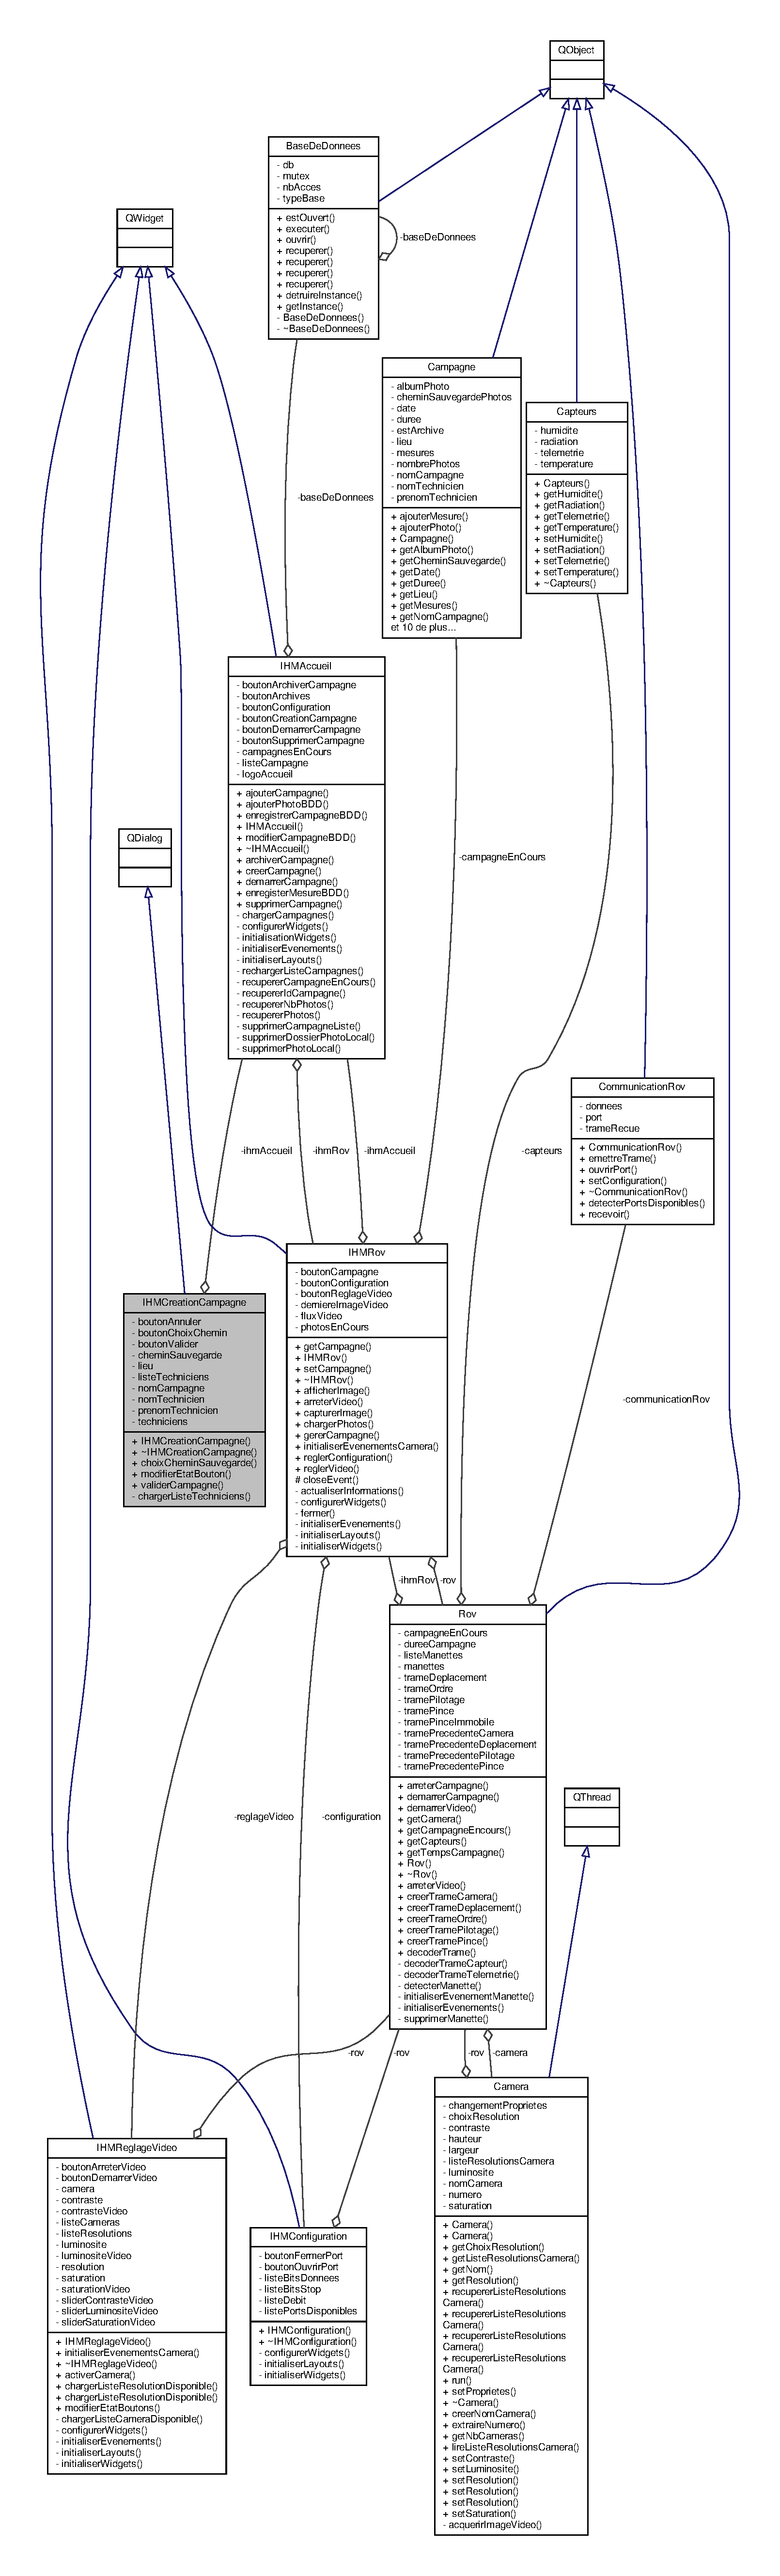
\includegraphics[height=550pt]{class_i_h_m_creation_campagne__coll__graph}
\end{center}
\end{figure}
\subsubsection*{Connecteurs publics}
\begin{DoxyCompactItemize}
\item 
void \hyperlink{class_i_h_m_creation_campagne_aceedbe44750998444120ae6343bbdcc6}{choix\+Chemin\+Sauvegarde} ()
\begin{DoxyCompactList}\small\item\em Permet de choisir le chemin de sauvegarde des photos. \end{DoxyCompactList}\item 
void \hyperlink{class_i_h_m_creation_campagne_a93395fef027960e7ab0d5c75a76e7414}{modifier\+Etat\+Bouton} (int index)
\begin{DoxyCompactList}\small\item\em Modifie l\textquotesingle{}état des boutons de la boite de dialogue \char`\"{}création d\textquotesingle{}une nouvelle campagne\char`\"{} si un technicien connue est choisi les ligne permettant de rentrer un nouveau technicien deviennent non-\/éditables. \end{DoxyCompactList}\item 
void \hyperlink{class_i_h_m_creation_campagne_ad5c63453b1b8d1099a43ff3522244072}{valider\+Campagne} ()
\begin{DoxyCompactList}\small\item\em Créer un nouvel objet \hyperlink{class_campagne}{Campagne} et l\textquotesingle{}ajoute dans la liste des campagnes disponibles. \end{DoxyCompactList}\end{DoxyCompactItemize}
\subsubsection*{Fonctions membres publiques}
\begin{DoxyCompactItemize}
\item 
\hyperlink{class_i_h_m_creation_campagne_a0e9cce2b950a638f1bf012b79d05eb9c}{I\+H\+M\+Creation\+Campagne} (\hyperlink{class_i_h_m_accueil}{I\+H\+M\+Accueil} $\ast$\hyperlink{class_i_h_m_creation_campagne_a6b5ea4a52138016a07a37060669288ae}{ihm\+Accueil}, Q\+Vector$<$ Q\+String\+List $>$ \&\hyperlink{class_i_h_m_creation_campagne_aee78d20f0263359283cbcbc50fac3143}{liste\+Techniciens})
\begin{DoxyCompactList}\small\item\em Constructeur de la classe \hyperlink{class_i_h_m_creation_campagne}{I\+H\+M\+Creation\+Campagne}. \end{DoxyCompactList}\item 
\hyperlink{class_i_h_m_creation_campagne_af2f85377637b15ccb2215b4b1f96b574}{$\sim$\+I\+H\+M\+Creation\+Campagne} ()
\begin{DoxyCompactList}\small\item\em Destructeur de la classe \hyperlink{class_i_h_m_creation_campagne}{I\+H\+M\+Creation\+Campagne}. \end{DoxyCompactList}\end{DoxyCompactItemize}
\subsubsection*{Fonctions membres privées}
\begin{DoxyCompactItemize}
\item 
void \hyperlink{class_i_h_m_creation_campagne_a0648a6013cec5557150d0addf30e2bbc}{charger\+Liste\+Techniciens} ()
\begin{DoxyCompactList}\small\item\em Charge la liste des techniciens connus de la bdd dans la liste déroulante. \end{DoxyCompactList}\end{DoxyCompactItemize}
\subsubsection*{Attributs privés}
\begin{DoxyCompactItemize}
\item 
Q\+Push\+Button $\ast$ \hyperlink{class_i_h_m_creation_campagne_ab20ebd5f09b98103c682ed2e1b192a1d}{bouton\+Annuler}
\begin{DoxyCompactList}\small\item\em Bouton permettant d\textquotesingle{}annuler la création de la campagne. \end{DoxyCompactList}\item 
Q\+Push\+Button $\ast$ \hyperlink{class_i_h_m_creation_campagne_ab709b06a83d8e1ebf9c920e7c60e2d79}{bouton\+Choix\+Chemin}
\begin{DoxyCompactList}\small\item\em Bouton permettant de choisir le chemin de sauvegarde des photos. \end{DoxyCompactList}\item 
Q\+Push\+Button $\ast$ \hyperlink{class_i_h_m_creation_campagne_a7c1dbc0141ba19b9ac16ea1444cd5d6f}{bouton\+Valider}
\begin{DoxyCompactList}\small\item\em Bouton permettant de valider la création de la campagne. \end{DoxyCompactList}\item 
Q\+Line\+Edit $\ast$ \hyperlink{class_i_h_m_creation_campagne_a95c12e2d42063f9c510704b87e3357da}{chemin\+Sauvegarde}
\begin{DoxyCompactList}\small\item\em Ligne editable permettant de choisir le chemin de sauvegarde des photos. \end{DoxyCompactList}\item 
\hyperlink{class_i_h_m_accueil}{I\+H\+M\+Accueil} $\ast$ \hyperlink{class_i_h_m_creation_campagne_a6b5ea4a52138016a07a37060669288ae}{ihm\+Accueil}
\begin{DoxyCompactList}\small\item\em Association avec la classe \hyperlink{class_i_h_m_accueil}{I\+H\+M\+Accueil}. \end{DoxyCompactList}\item 
Q\+Line\+Edit $\ast$ \hyperlink{class_i_h_m_creation_campagne_af68a722acc97a1011ff82752169a2ac8}{lieu}
\begin{DoxyCompactList}\small\item\em Ligne editable permettant de rentrer le lieu de la campagne à créer. \end{DoxyCompactList}\item 
Q\+Vector$<$ Q\+String\+List $>$ \hyperlink{class_i_h_m_creation_campagne_aee78d20f0263359283cbcbc50fac3143}{liste\+Techniciens}
\begin{DoxyCompactList}\small\item\em Conteneur de liste des informations des techniciens présent dans la base de données. \end{DoxyCompactList}\item 
Q\+Line\+Edit $\ast$ \hyperlink{class_i_h_m_creation_campagne_a6f07f2571a10f035c7b6a3ef1daefdab}{nom\+Campagne}
\begin{DoxyCompactList}\small\item\em Ligne editable permettant de rentrer le nom de la campagne à créer. \end{DoxyCompactList}\item 
Q\+Line\+Edit $\ast$ \hyperlink{class_i_h_m_creation_campagne_a5546fee9a51daceb1b719b105427dfe9}{nom\+Technicien}
\begin{DoxyCompactList}\small\item\em Ligne editable permettant de rentrer le nom du technicien à créer. \end{DoxyCompactList}\item 
Q\+Line\+Edit $\ast$ \hyperlink{class_i_h_m_creation_campagne_a95e0a4f224110a79731e947baa505b7e}{prenom\+Technicien}
\begin{DoxyCompactList}\small\item\em Ligne editable permettant de rentrer le prenom du technicien à créer. \end{DoxyCompactList}\item 
Q\+Combo\+Box $\ast$ \hyperlink{class_i_h_m_creation_campagne_a8235e7a18cda1298be624a59a4cc1a56}{techniciens}
\begin{DoxyCompactList}\small\item\em Liste déroulantes contenant tous les technicien connus. \end{DoxyCompactList}\end{DoxyCompactItemize}


\subsubsection{Description détaillée}
Class permettant de créer une nouvelle campagne. 

Définition à la ligne \hyperlink{ihmcreationcampagne_8h_source_l00022}{22} du fichier \hyperlink{ihmcreationcampagne_8h_source}{ihmcreationcampagne.\+h}.



\subsubsection{Documentation des constructeurs et destructeur}
\mbox{\Hypertarget{class_i_h_m_creation_campagne_a0e9cce2b950a638f1bf012b79d05eb9c}\label{class_i_h_m_creation_campagne_a0e9cce2b950a638f1bf012b79d05eb9c}} 
\index{I\+H\+M\+Creation\+Campagne@{I\+H\+M\+Creation\+Campagne}!I\+H\+M\+Creation\+Campagne@{I\+H\+M\+Creation\+Campagne}}
\index{I\+H\+M\+Creation\+Campagne@{I\+H\+M\+Creation\+Campagne}!I\+H\+M\+Creation\+Campagne@{I\+H\+M\+Creation\+Campagne}}
\paragraph{\texorpdfstring{I\+H\+M\+Creation\+Campagne()}{IHMCreationCampagne()}}
{\footnotesize\ttfamily I\+H\+M\+Creation\+Campagne\+::\+I\+H\+M\+Creation\+Campagne (\begin{DoxyParamCaption}\item[{\hyperlink{class_i_h_m_accueil}{I\+H\+M\+Accueil} $\ast$}]{ihm\+Accueil,  }\item[{Q\+Vector$<$ Q\+String\+List $>$ \&}]{liste\+Techniciens }\end{DoxyParamCaption})\hspace{0.3cm}{\ttfamily [explicit]}}



Constructeur de la classe \hyperlink{class_i_h_m_creation_campagne}{I\+H\+M\+Creation\+Campagne}. 


\begin{DoxyParams}{Paramètres}
{\em ihm\+Accueil} & \\
\hline
{\em liste\+Techniciens} & \\
\hline
\end{DoxyParams}


Définition à la ligne \hyperlink{ihmcreationcampagne_8cpp_source_l00011}{11} du fichier \hyperlink{ihmcreationcampagne_8cpp_source}{ihmcreationcampagne.\+cpp}.



Références \hyperlink{ihmcreationcampagne_8h_source_l00033}{bouton\+Annuler}, \hyperlink{ihmcreationcampagne_8h_source_l00034}{bouton\+Choix\+Chemin}, \hyperlink{ihmcreationcampagne_8h_source_l00032}{bouton\+Valider}, \hyperlink{ihmcreationcampagne_8cpp_source_l00061}{charger\+Liste\+Techniciens()}, \hyperlink{ihmcreationcampagne_8h_source_l00031}{chemin\+Sauvegarde}, \hyperlink{ihmcreationcampagne_8cpp_source_l00104}{choix\+Chemin\+Sauvegarde()}, \hyperlink{ihmcreationcampagne_8h_source_l00030}{lieu}, \hyperlink{ihmcreationcampagne_8cpp_source_l00086}{modifier\+Etat\+Bouton()}, \hyperlink{ihmcreationcampagne_8h_source_l00027}{nom\+Campagne}, \hyperlink{ihmcreationcampagne_8h_source_l00028}{nom\+Technicien}, \hyperlink{ihmcreationcampagne_8h_source_l00029}{prenom\+Technicien}, \hyperlink{ihmcreationcampagne_8h_source_l00035}{techniciens}, et \hyperlink{ihmcreationcampagne_8cpp_source_l00071}{valider\+Campagne()}.


\begin{DoxyCode}
00011                                                                                                        : 
      \hyperlink{class_q_dialog}{QDialog}(ihmAccueil, Qt::Dialog), \hyperlink{class_i_h_m_creation_campagne_a6b5ea4a52138016a07a37060669288ae}{ihmAccueil}(ihmAccueil), 
      \hyperlink{class_i_h_m_creation_campagne_aee78d20f0263359283cbcbc50fac3143}{listeTechniciens}(\hyperlink{class_i_h_m_creation_campagne_aee78d20f0263359283cbcbc50fac3143}{listeTechniciens})
00012 \{
00013     qDebug() << Q\_FUNC\_INFO;
00014     \hyperlink{class_i_h_m_creation_campagne_a6f07f2571a10f035c7b6a3ef1daefdab}{nomCampagne} = \textcolor{keyword}{new} QLineEdit(\textcolor{keyword}{this});
00015     \hyperlink{class_i_h_m_creation_campagne_a5546fee9a51daceb1b719b105427dfe9}{nomTechnicien} = \textcolor{keyword}{new} QLineEdit(\textcolor{keyword}{this});
00016     \hyperlink{class_i_h_m_creation_campagne_a95e0a4f224110a79731e947baa505b7e}{prenomTechnicien} = \textcolor{keyword}{new} QLineEdit(\textcolor{keyword}{this});
00017     \hyperlink{class_i_h_m_creation_campagne_af68a722acc97a1011ff82752169a2ac8}{lieu} = \textcolor{keyword}{new} QLineEdit(\textcolor{keyword}{this});
00018     \hyperlink{class_i_h_m_creation_campagne_a95c12e2d42063f9c510704b87e3357da}{cheminSauvegarde} = \textcolor{keyword}{new} QLineEdit(\textcolor{keyword}{this});
00019     \hyperlink{class_i_h_m_creation_campagne_a7c1dbc0141ba19b9ac16ea1444cd5d6f}{boutonValider} = \textcolor{keyword}{new} QPushButton(\textcolor{stringliteral}{"Valider"}, \textcolor{keyword}{this});
00020     \hyperlink{class_i_h_m_creation_campagne_ab20ebd5f09b98103c682ed2e1b192a1d}{boutonAnnuler} = \textcolor{keyword}{new} QPushButton(\textcolor{stringliteral}{"Annuler"}, \textcolor{keyword}{this});
00021     \hyperlink{class_i_h_m_creation_campagne_ab709b06a83d8e1ebf9c920e7c60e2d79}{boutonChoixChemin} = \textcolor{keyword}{new} QPushButton(\textcolor{stringliteral}{"..."}, \textcolor{keyword}{this});
00022     \hyperlink{class_i_h_m_creation_campagne_a8235e7a18cda1298be624a59a4cc1a56}{techniciens} = \textcolor{keyword}{new} QComboBox(\textcolor{keyword}{this});
00023 
00024     QVBoxLayout *layoutPrincipal = \textcolor{keyword}{new} QVBoxLayout;
00025     QFormLayout *layoutFormulaireCampagne = \textcolor{keyword}{new} QFormLayout;
00026     QHBoxLayout *layoutValidation = \textcolor{keyword}{new} QHBoxLayout;
00027     QHBoxLayout *layoutChoixChemin = \textcolor{keyword}{new} QHBoxLayout;
00028 
00029     layoutPrincipal->addLayout(layoutFormulaireCampagne);
00030     layoutPrincipal->addLayout(layoutValidation);
00031     layoutChoixChemin->addWidget(\hyperlink{class_i_h_m_creation_campagne_a95c12e2d42063f9c510704b87e3357da}{cheminSauvegarde});
00032     layoutChoixChemin->addWidget(\hyperlink{class_i_h_m_creation_campagne_ab709b06a83d8e1ebf9c920e7c60e2d79}{boutonChoixChemin});
00033 
00034     layoutFormulaireCampagne->addRow(\textcolor{stringliteral}{"Nom campagne : "}, \hyperlink{class_i_h_m_creation_campagne_a6f07f2571a10f035c7b6a3ef1daefdab}{nomCampagne});
00035     layoutFormulaireCampagne->addRow(\textcolor{stringliteral}{"Techniciens : "}, \hyperlink{class_i_h_m_creation_campagne_a8235e7a18cda1298be624a59a4cc1a56}{techniciens});
00036     layoutFormulaireCampagne->addRow(\textcolor{stringliteral}{"Nom technicien : "}, \hyperlink{class_i_h_m_creation_campagne_a5546fee9a51daceb1b719b105427dfe9}{nomTechnicien});
00037     layoutFormulaireCampagne->addRow(\textcolor{stringliteral}{"Prenom technicien : "}, \hyperlink{class_i_h_m_creation_campagne_a95e0a4f224110a79731e947baa505b7e}{prenomTechnicien});
00038     layoutFormulaireCampagne->addRow(\textcolor{stringliteral}{"Lieu campagne : "}, \hyperlink{class_i_h_m_creation_campagne_af68a722acc97a1011ff82752169a2ac8}{lieu});
00039     layoutFormulaireCampagne->addRow(\textcolor{stringliteral}{"Chemin sauvegarde photos : "}, layoutChoixChemin);
00040 
00041     layoutValidation->addWidget(\hyperlink{class_i_h_m_creation_campagne_a7c1dbc0141ba19b9ac16ea1444cd5d6f}{boutonValider});
00042     layoutValidation->addWidget(\hyperlink{class_i_h_m_creation_campagne_ab20ebd5f09b98103c682ed2e1b192a1d}{boutonAnnuler});
00043 
00044     layoutValidation->setAlignment(Qt::AlignBottom);
00045 
00046     setLayout(layoutPrincipal);
00047 
00048     connect(\hyperlink{class_i_h_m_creation_campagne_a7c1dbc0141ba19b9ac16ea1444cd5d6f}{boutonValider}, SIGNAL(clicked()), \textcolor{keyword}{this}, SLOT(
      \hyperlink{class_i_h_m_creation_campagne_ad5c63453b1b8d1099a43ff3522244072}{validerCampagne}()));
00049     connect(\hyperlink{class_i_h_m_creation_campagne_ab20ebd5f09b98103c682ed2e1b192a1d}{boutonAnnuler}, SIGNAL(clicked()), \textcolor{keyword}{this}, SLOT(close()));
00050     connect(\hyperlink{class_i_h_m_creation_campagne_ab709b06a83d8e1ebf9c920e7c60e2d79}{boutonChoixChemin}, SIGNAL(clicked()), \textcolor{keyword}{this}, SLOT(
      \hyperlink{class_i_h_m_creation_campagne_aceedbe44750998444120ae6343bbdcc6}{choixCheminSauvegarde}()));
00051     connect(\hyperlink{class_i_h_m_creation_campagne_a8235e7a18cda1298be624a59a4cc1a56}{techniciens}, SIGNAL(currentIndexChanged(\textcolor{keywordtype}{int})), \textcolor{keyword}{this}, SLOT(
      \hyperlink{class_i_h_m_creation_campagne_a93395fef027960e7ab0d5c75a76e7414}{modifierEtatBouton}(\textcolor{keywordtype}{int})));
00052 
00053     \hyperlink{class_i_h_m_creation_campagne_a0648a6013cec5557150d0addf30e2bbc}{chargerListeTechniciens}();
00054 \}
\end{DoxyCode}
\mbox{\Hypertarget{class_i_h_m_creation_campagne_af2f85377637b15ccb2215b4b1f96b574}\label{class_i_h_m_creation_campagne_af2f85377637b15ccb2215b4b1f96b574}} 
\index{I\+H\+M\+Creation\+Campagne@{I\+H\+M\+Creation\+Campagne}!````~I\+H\+M\+Creation\+Campagne@{$\sim$\+I\+H\+M\+Creation\+Campagne}}
\index{````~I\+H\+M\+Creation\+Campagne@{$\sim$\+I\+H\+M\+Creation\+Campagne}!I\+H\+M\+Creation\+Campagne@{I\+H\+M\+Creation\+Campagne}}
\paragraph{\texorpdfstring{$\sim$\+I\+H\+M\+Creation\+Campagne()}{~IHMCreationCampagne()}}
{\footnotesize\ttfamily I\+H\+M\+Creation\+Campagne\+::$\sim$\+I\+H\+M\+Creation\+Campagne (\begin{DoxyParamCaption}{ }\end{DoxyParamCaption})}



Destructeur de la classe \hyperlink{class_i_h_m_creation_campagne}{I\+H\+M\+Creation\+Campagne}. 



Définition à la ligne \hyperlink{ihmcreationcampagne_8cpp_source_l00056}{56} du fichier \hyperlink{ihmcreationcampagne_8cpp_source}{ihmcreationcampagne.\+cpp}.


\begin{DoxyCode}
00057 \{
00058     qDebug() << Q\_FUNC\_INFO;
00059 \}
\end{DoxyCode}


\subsubsection{Documentation des fonctions membres}
\mbox{\Hypertarget{class_i_h_m_creation_campagne_a0648a6013cec5557150d0addf30e2bbc}\label{class_i_h_m_creation_campagne_a0648a6013cec5557150d0addf30e2bbc}} 
\index{I\+H\+M\+Creation\+Campagne@{I\+H\+M\+Creation\+Campagne}!charger\+Liste\+Techniciens@{charger\+Liste\+Techniciens}}
\index{charger\+Liste\+Techniciens@{charger\+Liste\+Techniciens}!I\+H\+M\+Creation\+Campagne@{I\+H\+M\+Creation\+Campagne}}
\paragraph{\texorpdfstring{charger\+Liste\+Techniciens()}{chargerListeTechniciens()}}
{\footnotesize\ttfamily void I\+H\+M\+Creation\+Campagne\+::charger\+Liste\+Techniciens (\begin{DoxyParamCaption}{ }\end{DoxyParamCaption})\hspace{0.3cm}{\ttfamily [private]}}



Charge la liste des techniciens connus de la bdd dans la liste déroulante. 



Définition à la ligne \hyperlink{ihmcreationcampagne_8cpp_source_l00061}{61} du fichier \hyperlink{ihmcreationcampagne_8cpp_source}{ihmcreationcampagne.\+cpp}.



Références \hyperlink{ihmcreationcampagne_8h_source_l00036}{liste\+Techniciens}, et \hyperlink{ihmcreationcampagne_8h_source_l00035}{techniciens}.



Référencé par \hyperlink{ihmcreationcampagne_8cpp_source_l00011}{I\+H\+M\+Creation\+Campagne()}.


\begin{DoxyCode}
00062 \{
00063     \hyperlink{class_i_h_m_creation_campagne_a8235e7a18cda1298be624a59a4cc1a56}{techniciens}->addItem(\textcolor{stringliteral}{"Ajouter technicien"});
00064 
00065     \textcolor{keywordflow}{for}(QVector<QStringList>::iterator it = \hyperlink{class_i_h_m_creation_campagne_aee78d20f0263359283cbcbc50fac3143}{listeTechniciens}.begin(); it != 
      \hyperlink{class_i_h_m_creation_campagne_aee78d20f0263359283cbcbc50fac3143}{listeTechniciens}.end(); ++it)
00066     \{
00067         \hyperlink{class_i_h_m_creation_campagne_a8235e7a18cda1298be624a59a4cc1a56}{techniciens}->addItem((*it).at(0) + \textcolor{stringliteral}{" "} + (*it).at(1));
00068     \}
00069 \}
\end{DoxyCode}
\mbox{\Hypertarget{class_i_h_m_creation_campagne_aceedbe44750998444120ae6343bbdcc6}\label{class_i_h_m_creation_campagne_aceedbe44750998444120ae6343bbdcc6}} 
\index{I\+H\+M\+Creation\+Campagne@{I\+H\+M\+Creation\+Campagne}!choix\+Chemin\+Sauvegarde@{choix\+Chemin\+Sauvegarde}}
\index{choix\+Chemin\+Sauvegarde@{choix\+Chemin\+Sauvegarde}!I\+H\+M\+Creation\+Campagne@{I\+H\+M\+Creation\+Campagne}}
\paragraph{\texorpdfstring{choix\+Chemin\+Sauvegarde}{choixCheminSauvegarde}}
{\footnotesize\ttfamily void I\+H\+M\+Creation\+Campagne\+::choix\+Chemin\+Sauvegarde (\begin{DoxyParamCaption}{ }\end{DoxyParamCaption})\hspace{0.3cm}{\ttfamily [slot]}}



Permet de choisir le chemin de sauvegarde des photos. 



Définition à la ligne \hyperlink{ihmcreationcampagne_8cpp_source_l00104}{104} du fichier \hyperlink{ihmcreationcampagne_8cpp_source}{ihmcreationcampagne.\+cpp}.



Références \hyperlink{ihmcreationcampagne_8h_source_l00031}{chemin\+Sauvegarde}.



Référencé par \hyperlink{ihmcreationcampagne_8cpp_source_l00011}{I\+H\+M\+Creation\+Campagne()}.


\begin{DoxyCode}
00105 \{
00106     \hyperlink{class_i_h_m_creation_campagne_a95c12e2d42063f9c510704b87e3357da}{cheminSauvegarde}->setText(QFileDialog::getExistingDirectory(\textcolor{keyword}{this}, \textcolor{stringliteral}{"Choix du chemin de
       sauvegarde des photos"}));
00107 \}
\end{DoxyCode}
\mbox{\Hypertarget{class_i_h_m_creation_campagne_a93395fef027960e7ab0d5c75a76e7414}\label{class_i_h_m_creation_campagne_a93395fef027960e7ab0d5c75a76e7414}} 
\index{I\+H\+M\+Creation\+Campagne@{I\+H\+M\+Creation\+Campagne}!modifier\+Etat\+Bouton@{modifier\+Etat\+Bouton}}
\index{modifier\+Etat\+Bouton@{modifier\+Etat\+Bouton}!I\+H\+M\+Creation\+Campagne@{I\+H\+M\+Creation\+Campagne}}
\paragraph{\texorpdfstring{modifier\+Etat\+Bouton}{modifierEtatBouton}}
{\footnotesize\ttfamily void I\+H\+M\+Creation\+Campagne\+::modifier\+Etat\+Bouton (\begin{DoxyParamCaption}\item[{int}]{index }\end{DoxyParamCaption})\hspace{0.3cm}{\ttfamily [slot]}}



Modifie l\textquotesingle{}état des boutons de la boite de dialogue \char`\"{}création d\textquotesingle{}une nouvelle campagne\char`\"{} si un technicien connue est choisi les ligne permettant de rentrer un nouveau technicien deviennent non-\/éditables. 


\begin{DoxyParams}{Paramètres}
{\em index} & \\
\hline
\end{DoxyParams}


Définition à la ligne \hyperlink{ihmcreationcampagne_8cpp_source_l00086}{86} du fichier \hyperlink{ihmcreationcampagne_8cpp_source}{ihmcreationcampagne.\+cpp}.



Références \hyperlink{ihmcreationcampagne_8h_source_l00036}{liste\+Techniciens}, \hyperlink{ihmcreationcampagne_8h_source_l00028}{nom\+Technicien}, et \hyperlink{ihmcreationcampagne_8h_source_l00029}{prenom\+Technicien}.



Référencé par \hyperlink{ihmcreationcampagne_8cpp_source_l00011}{I\+H\+M\+Creation\+Campagne()}.


\begin{DoxyCode}
00087 \{
00088     \textcolor{keywordflow}{if}(index > 0)
00089     \{
00090         \hyperlink{class_i_h_m_creation_campagne_a5546fee9a51daceb1b719b105427dfe9}{nomTechnicien}->setDisabled(\textcolor{keyword}{true});
00091         \hyperlink{class_i_h_m_creation_campagne_a5546fee9a51daceb1b719b105427dfe9}{nomTechnicien}->setText(\hyperlink{class_i_h_m_creation_campagne_aee78d20f0263359283cbcbc50fac3143}{listeTechniciens}[index - 1].at(0));
00092         \hyperlink{class_i_h_m_creation_campagne_a95e0a4f224110a79731e947baa505b7e}{prenomTechnicien}->setDisabled(\textcolor{keyword}{true});
00093         \hyperlink{class_i_h_m_creation_campagne_a95e0a4f224110a79731e947baa505b7e}{prenomTechnicien}->setText(\hyperlink{class_i_h_m_creation_campagne_aee78d20f0263359283cbcbc50fac3143}{listeTechniciens}[index - 1].at(1));
00094     \}
00095     \textcolor{keywordflow}{else}
00096     \{
00097         \hyperlink{class_i_h_m_creation_campagne_a5546fee9a51daceb1b719b105427dfe9}{nomTechnicien}->clear();
00098         \hyperlink{class_i_h_m_creation_campagne_a95e0a4f224110a79731e947baa505b7e}{prenomTechnicien}->clear();
00099         \hyperlink{class_i_h_m_creation_campagne_a5546fee9a51daceb1b719b105427dfe9}{nomTechnicien}->setEnabled(\textcolor{keyword}{true});
00100         \hyperlink{class_i_h_m_creation_campagne_a95e0a4f224110a79731e947baa505b7e}{prenomTechnicien}->setEnabled(\textcolor{keyword}{true});
00101     \}
00102 \}
\end{DoxyCode}
\mbox{\Hypertarget{class_i_h_m_creation_campagne_ad5c63453b1b8d1099a43ff3522244072}\label{class_i_h_m_creation_campagne_ad5c63453b1b8d1099a43ff3522244072}} 
\index{I\+H\+M\+Creation\+Campagne@{I\+H\+M\+Creation\+Campagne}!valider\+Campagne@{valider\+Campagne}}
\index{valider\+Campagne@{valider\+Campagne}!I\+H\+M\+Creation\+Campagne@{I\+H\+M\+Creation\+Campagne}}
\paragraph{\texorpdfstring{valider\+Campagne}{validerCampagne}}
{\footnotesize\ttfamily void I\+H\+M\+Creation\+Campagne\+::valider\+Campagne (\begin{DoxyParamCaption}{ }\end{DoxyParamCaption})\hspace{0.3cm}{\ttfamily [slot]}}



Créer un nouvel objet \hyperlink{class_campagne}{Campagne} et l\textquotesingle{}ajoute dans la liste des campagnes disponibles. 



Définition à la ligne \hyperlink{ihmcreationcampagne_8cpp_source_l00071}{71} du fichier \hyperlink{ihmcreationcampagne_8cpp_source}{ihmcreationcampagne.\+cpp}.



Références \hyperlink{ihmaccueil_8cpp_source_l00254}{I\+H\+M\+Accueil\+::ajouter\+Campagne()}, \hyperlink{ihmcreationcampagne_8h_source_l00031}{chemin\+Sauvegarde}, \hyperlink{ihmaccueil_8cpp_source_l00273}{I\+H\+M\+Accueil\+::enregistrer\+Campagne\+B\+D\+D()}, \hyperlink{ihmcreationcampagne_8h_source_l00026}{ihm\+Accueil}, \hyperlink{ihmcreationcampagne_8h_source_l00030}{lieu}, \hyperlink{ihmcreationcampagne_8h_source_l00027}{nom\+Campagne}, \hyperlink{ihmcreationcampagne_8h_source_l00028}{nom\+Technicien}, \hyperlink{ihmcreationcampagne_8h_source_l00029}{prenom\+Technicien}, et \hyperlink{campagne_8cpp_source_l00060}{Campagne\+::set\+Chemin\+Sauvegarde()}.



Référencé par \hyperlink{ihmcreationcampagne_8cpp_source_l00011}{I\+H\+M\+Creation\+Campagne()}.


\begin{DoxyCode}
00072 \{
00073     \textcolor{keywordflow}{if}(\hyperlink{class_i_h_m_creation_campagne_a6f07f2571a10f035c7b6a3ef1daefdab}{nomCampagne}->text().isEmpty() || \hyperlink{class_i_h_m_creation_campagne_a5546fee9a51daceb1b719b105427dfe9}{nomTechnicien}->text().isEmpty() || 
      \hyperlink{class_i_h_m_creation_campagne_a95e0a4f224110a79731e947baa505b7e}{prenomTechnicien}->text().isEmpty() || \hyperlink{class_i_h_m_creation_campagne_af68a722acc97a1011ff82752169a2ac8}{lieu}->text().isEmpty() || 
      \hyperlink{class_i_h_m_creation_campagne_a95c12e2d42063f9c510704b87e3357da}{cheminSauvegarde}->text().isEmpty())
00074     \{
00075         QMessageBox::critical(\textcolor{keyword}{nullptr}, \textcolor{stringliteral}{"Création campagne"}, \textcolor{stringliteral}{"Informations incomplètes !"});
00076         \textcolor{keywordflow}{return};
00077     \}
00078 
00079     \hyperlink{class_campagne}{Campagne} *campagne = \textcolor{keyword}{new} \hyperlink{class_campagne}{Campagne}(\hyperlink{class_i_h_m_creation_campagne_a6f07f2571a10f035c7b6a3ef1daefdab}{nomCampagne}->text(), 
      \hyperlink{class_i_h_m_creation_campagne_af68a722acc97a1011ff82752169a2ac8}{lieu}->text(), \hyperlink{class_i_h_m_creation_campagne_a5546fee9a51daceb1b719b105427dfe9}{nomTechnicien}->text(), \hyperlink{class_i_h_m_creation_campagne_a95e0a4f224110a79731e947baa505b7e}{prenomTechnicien}->text(), 
      QDateTime::currentDateTime(), \textcolor{keyword}{this});
00080     campagne->\hyperlink{class_campagne_a68c7eb6776e46306b10f1ca2a409ae6e}{setCheminSauvegarde}(\hyperlink{class_i_h_m_creation_campagne_a95c12e2d42063f9c510704b87e3357da}{cheminSauvegarde}->text());
00081     \hyperlink{class_i_h_m_creation_campagne_a6b5ea4a52138016a07a37060669288ae}{ihmAccueil}->\hyperlink{class_i_h_m_accueil_a3087ce7a78561c79ce3148761750dd1d}{ajouterCampagne}(campagne, \textcolor{keyword}{true});
00082     \hyperlink{class_i_h_m_creation_campagne_a6b5ea4a52138016a07a37060669288ae}{ihmAccueil}->\hyperlink{class_i_h_m_accueil_a5ab04fc3fa87817bec130f377d563b75}{enregistrerCampagneBDD}(campagne);
00083     close();
00084 \}
\end{DoxyCode}


\subsubsection{Documentation des données membres}
\mbox{\Hypertarget{class_i_h_m_creation_campagne_ab20ebd5f09b98103c682ed2e1b192a1d}\label{class_i_h_m_creation_campagne_ab20ebd5f09b98103c682ed2e1b192a1d}} 
\index{I\+H\+M\+Creation\+Campagne@{I\+H\+M\+Creation\+Campagne}!bouton\+Annuler@{bouton\+Annuler}}
\index{bouton\+Annuler@{bouton\+Annuler}!I\+H\+M\+Creation\+Campagne@{I\+H\+M\+Creation\+Campagne}}
\paragraph{\texorpdfstring{bouton\+Annuler}{boutonAnnuler}}
{\footnotesize\ttfamily Q\+Push\+Button$\ast$ I\+H\+M\+Creation\+Campagne\+::bouton\+Annuler\hspace{0.3cm}{\ttfamily [private]}}



Bouton permettant d\textquotesingle{}annuler la création de la campagne. 



Définition à la ligne \hyperlink{ihmcreationcampagne_8h_source_l00033}{33} du fichier \hyperlink{ihmcreationcampagne_8h_source}{ihmcreationcampagne.\+h}.



Référencé par \hyperlink{ihmcreationcampagne_8cpp_source_l00011}{I\+H\+M\+Creation\+Campagne()}.

\mbox{\Hypertarget{class_i_h_m_creation_campagne_ab709b06a83d8e1ebf9c920e7c60e2d79}\label{class_i_h_m_creation_campagne_ab709b06a83d8e1ebf9c920e7c60e2d79}} 
\index{I\+H\+M\+Creation\+Campagne@{I\+H\+M\+Creation\+Campagne}!bouton\+Choix\+Chemin@{bouton\+Choix\+Chemin}}
\index{bouton\+Choix\+Chemin@{bouton\+Choix\+Chemin}!I\+H\+M\+Creation\+Campagne@{I\+H\+M\+Creation\+Campagne}}
\paragraph{\texorpdfstring{bouton\+Choix\+Chemin}{boutonChoixChemin}}
{\footnotesize\ttfamily Q\+Push\+Button$\ast$ I\+H\+M\+Creation\+Campagne\+::bouton\+Choix\+Chemin\hspace{0.3cm}{\ttfamily [private]}}



Bouton permettant de choisir le chemin de sauvegarde des photos. 



Définition à la ligne \hyperlink{ihmcreationcampagne_8h_source_l00034}{34} du fichier \hyperlink{ihmcreationcampagne_8h_source}{ihmcreationcampagne.\+h}.



Référencé par \hyperlink{ihmcreationcampagne_8cpp_source_l00011}{I\+H\+M\+Creation\+Campagne()}.

\mbox{\Hypertarget{class_i_h_m_creation_campagne_a7c1dbc0141ba19b9ac16ea1444cd5d6f}\label{class_i_h_m_creation_campagne_a7c1dbc0141ba19b9ac16ea1444cd5d6f}} 
\index{I\+H\+M\+Creation\+Campagne@{I\+H\+M\+Creation\+Campagne}!bouton\+Valider@{bouton\+Valider}}
\index{bouton\+Valider@{bouton\+Valider}!I\+H\+M\+Creation\+Campagne@{I\+H\+M\+Creation\+Campagne}}
\paragraph{\texorpdfstring{bouton\+Valider}{boutonValider}}
{\footnotesize\ttfamily Q\+Push\+Button$\ast$ I\+H\+M\+Creation\+Campagne\+::bouton\+Valider\hspace{0.3cm}{\ttfamily [private]}}



Bouton permettant de valider la création de la campagne. 



Définition à la ligne \hyperlink{ihmcreationcampagne_8h_source_l00032}{32} du fichier \hyperlink{ihmcreationcampagne_8h_source}{ihmcreationcampagne.\+h}.



Référencé par \hyperlink{ihmcreationcampagne_8cpp_source_l00011}{I\+H\+M\+Creation\+Campagne()}.

\mbox{\Hypertarget{class_i_h_m_creation_campagne_a95c12e2d42063f9c510704b87e3357da}\label{class_i_h_m_creation_campagne_a95c12e2d42063f9c510704b87e3357da}} 
\index{I\+H\+M\+Creation\+Campagne@{I\+H\+M\+Creation\+Campagne}!chemin\+Sauvegarde@{chemin\+Sauvegarde}}
\index{chemin\+Sauvegarde@{chemin\+Sauvegarde}!I\+H\+M\+Creation\+Campagne@{I\+H\+M\+Creation\+Campagne}}
\paragraph{\texorpdfstring{chemin\+Sauvegarde}{cheminSauvegarde}}
{\footnotesize\ttfamily Q\+Line\+Edit$\ast$ I\+H\+M\+Creation\+Campagne\+::chemin\+Sauvegarde\hspace{0.3cm}{\ttfamily [private]}}



Ligne editable permettant de choisir le chemin de sauvegarde des photos. 



Définition à la ligne \hyperlink{ihmcreationcampagne_8h_source_l00031}{31} du fichier \hyperlink{ihmcreationcampagne_8h_source}{ihmcreationcampagne.\+h}.



Référencé par \hyperlink{ihmcreationcampagne_8cpp_source_l00104}{choix\+Chemin\+Sauvegarde()}, \hyperlink{ihmcreationcampagne_8cpp_source_l00011}{I\+H\+M\+Creation\+Campagne()}, et \hyperlink{ihmcreationcampagne_8cpp_source_l00071}{valider\+Campagne()}.

\mbox{\Hypertarget{class_i_h_m_creation_campagne_a6b5ea4a52138016a07a37060669288ae}\label{class_i_h_m_creation_campagne_a6b5ea4a52138016a07a37060669288ae}} 
\index{I\+H\+M\+Creation\+Campagne@{I\+H\+M\+Creation\+Campagne}!ihm\+Accueil@{ihm\+Accueil}}
\index{ihm\+Accueil@{ihm\+Accueil}!I\+H\+M\+Creation\+Campagne@{I\+H\+M\+Creation\+Campagne}}
\paragraph{\texorpdfstring{ihm\+Accueil}{ihmAccueil}}
{\footnotesize\ttfamily \hyperlink{class_i_h_m_accueil}{I\+H\+M\+Accueil}$\ast$ I\+H\+M\+Creation\+Campagne\+::ihm\+Accueil\hspace{0.3cm}{\ttfamily [private]}}



Association avec la classe \hyperlink{class_i_h_m_accueil}{I\+H\+M\+Accueil}. 



Définition à la ligne \hyperlink{ihmcreationcampagne_8h_source_l00026}{26} du fichier \hyperlink{ihmcreationcampagne_8h_source}{ihmcreationcampagne.\+h}.



Référencé par \hyperlink{ihmcreationcampagne_8cpp_source_l00071}{valider\+Campagne()}.

\mbox{\Hypertarget{class_i_h_m_creation_campagne_af68a722acc97a1011ff82752169a2ac8}\label{class_i_h_m_creation_campagne_af68a722acc97a1011ff82752169a2ac8}} 
\index{I\+H\+M\+Creation\+Campagne@{I\+H\+M\+Creation\+Campagne}!lieu@{lieu}}
\index{lieu@{lieu}!I\+H\+M\+Creation\+Campagne@{I\+H\+M\+Creation\+Campagne}}
\paragraph{\texorpdfstring{lieu}{lieu}}
{\footnotesize\ttfamily Q\+Line\+Edit$\ast$ I\+H\+M\+Creation\+Campagne\+::lieu\hspace{0.3cm}{\ttfamily [private]}}



Ligne editable permettant de rentrer le lieu de la campagne à créer. 



Définition à la ligne \hyperlink{ihmcreationcampagne_8h_source_l00030}{30} du fichier \hyperlink{ihmcreationcampagne_8h_source}{ihmcreationcampagne.\+h}.



Référencé par \hyperlink{ihmcreationcampagne_8cpp_source_l00011}{I\+H\+M\+Creation\+Campagne()}, et \hyperlink{ihmcreationcampagne_8cpp_source_l00071}{valider\+Campagne()}.

\mbox{\Hypertarget{class_i_h_m_creation_campagne_aee78d20f0263359283cbcbc50fac3143}\label{class_i_h_m_creation_campagne_aee78d20f0263359283cbcbc50fac3143}} 
\index{I\+H\+M\+Creation\+Campagne@{I\+H\+M\+Creation\+Campagne}!liste\+Techniciens@{liste\+Techniciens}}
\index{liste\+Techniciens@{liste\+Techniciens}!I\+H\+M\+Creation\+Campagne@{I\+H\+M\+Creation\+Campagne}}
\paragraph{\texorpdfstring{liste\+Techniciens}{listeTechniciens}}
{\footnotesize\ttfamily Q\+Vector$<$Q\+String\+List$>$ I\+H\+M\+Creation\+Campagne\+::liste\+Techniciens\hspace{0.3cm}{\ttfamily [private]}}



Conteneur de liste des informations des techniciens présent dans la base de données. 



Définition à la ligne \hyperlink{ihmcreationcampagne_8h_source_l00036}{36} du fichier \hyperlink{ihmcreationcampagne_8h_source}{ihmcreationcampagne.\+h}.



Référencé par \hyperlink{ihmcreationcampagne_8cpp_source_l00061}{charger\+Liste\+Techniciens()}, et \hyperlink{ihmcreationcampagne_8cpp_source_l00086}{modifier\+Etat\+Bouton()}.

\mbox{\Hypertarget{class_i_h_m_creation_campagne_a6f07f2571a10f035c7b6a3ef1daefdab}\label{class_i_h_m_creation_campagne_a6f07f2571a10f035c7b6a3ef1daefdab}} 
\index{I\+H\+M\+Creation\+Campagne@{I\+H\+M\+Creation\+Campagne}!nom\+Campagne@{nom\+Campagne}}
\index{nom\+Campagne@{nom\+Campagne}!I\+H\+M\+Creation\+Campagne@{I\+H\+M\+Creation\+Campagne}}
\paragraph{\texorpdfstring{nom\+Campagne}{nomCampagne}}
{\footnotesize\ttfamily Q\+Line\+Edit$\ast$ I\+H\+M\+Creation\+Campagne\+::nom\+Campagne\hspace{0.3cm}{\ttfamily [private]}}



Ligne editable permettant de rentrer le nom de la campagne à créer. 



Définition à la ligne \hyperlink{ihmcreationcampagne_8h_source_l00027}{27} du fichier \hyperlink{ihmcreationcampagne_8h_source}{ihmcreationcampagne.\+h}.



Référencé par \hyperlink{ihmcreationcampagne_8cpp_source_l00011}{I\+H\+M\+Creation\+Campagne()}, et \hyperlink{ihmcreationcampagne_8cpp_source_l00071}{valider\+Campagne()}.

\mbox{\Hypertarget{class_i_h_m_creation_campagne_a5546fee9a51daceb1b719b105427dfe9}\label{class_i_h_m_creation_campagne_a5546fee9a51daceb1b719b105427dfe9}} 
\index{I\+H\+M\+Creation\+Campagne@{I\+H\+M\+Creation\+Campagne}!nom\+Technicien@{nom\+Technicien}}
\index{nom\+Technicien@{nom\+Technicien}!I\+H\+M\+Creation\+Campagne@{I\+H\+M\+Creation\+Campagne}}
\paragraph{\texorpdfstring{nom\+Technicien}{nomTechnicien}}
{\footnotesize\ttfamily Q\+Line\+Edit$\ast$ I\+H\+M\+Creation\+Campagne\+::nom\+Technicien\hspace{0.3cm}{\ttfamily [private]}}



Ligne editable permettant de rentrer le nom du technicien à créer. 



Définition à la ligne \hyperlink{ihmcreationcampagne_8h_source_l00028}{28} du fichier \hyperlink{ihmcreationcampagne_8h_source}{ihmcreationcampagne.\+h}.



Référencé par \hyperlink{ihmcreationcampagne_8cpp_source_l00011}{I\+H\+M\+Creation\+Campagne()}, \hyperlink{ihmcreationcampagne_8cpp_source_l00086}{modifier\+Etat\+Bouton()}, et \hyperlink{ihmcreationcampagne_8cpp_source_l00071}{valider\+Campagne()}.

\mbox{\Hypertarget{class_i_h_m_creation_campagne_a95e0a4f224110a79731e947baa505b7e}\label{class_i_h_m_creation_campagne_a95e0a4f224110a79731e947baa505b7e}} 
\index{I\+H\+M\+Creation\+Campagne@{I\+H\+M\+Creation\+Campagne}!prenom\+Technicien@{prenom\+Technicien}}
\index{prenom\+Technicien@{prenom\+Technicien}!I\+H\+M\+Creation\+Campagne@{I\+H\+M\+Creation\+Campagne}}
\paragraph{\texorpdfstring{prenom\+Technicien}{prenomTechnicien}}
{\footnotesize\ttfamily Q\+Line\+Edit$\ast$ I\+H\+M\+Creation\+Campagne\+::prenom\+Technicien\hspace{0.3cm}{\ttfamily [private]}}



Ligne editable permettant de rentrer le prenom du technicien à créer. 



Définition à la ligne \hyperlink{ihmcreationcampagne_8h_source_l00029}{29} du fichier \hyperlink{ihmcreationcampagne_8h_source}{ihmcreationcampagne.\+h}.



Référencé par \hyperlink{ihmcreationcampagne_8cpp_source_l00011}{I\+H\+M\+Creation\+Campagne()}, \hyperlink{ihmcreationcampagne_8cpp_source_l00086}{modifier\+Etat\+Bouton()}, et \hyperlink{ihmcreationcampagne_8cpp_source_l00071}{valider\+Campagne()}.

\mbox{\Hypertarget{class_i_h_m_creation_campagne_a8235e7a18cda1298be624a59a4cc1a56}\label{class_i_h_m_creation_campagne_a8235e7a18cda1298be624a59a4cc1a56}} 
\index{I\+H\+M\+Creation\+Campagne@{I\+H\+M\+Creation\+Campagne}!techniciens@{techniciens}}
\index{techniciens@{techniciens}!I\+H\+M\+Creation\+Campagne@{I\+H\+M\+Creation\+Campagne}}
\paragraph{\texorpdfstring{techniciens}{techniciens}}
{\footnotesize\ttfamily Q\+Combo\+Box$\ast$ I\+H\+M\+Creation\+Campagne\+::techniciens\hspace{0.3cm}{\ttfamily [private]}}



Liste déroulantes contenant tous les technicien connus. 



Définition à la ligne \hyperlink{ihmcreationcampagne_8h_source_l00035}{35} du fichier \hyperlink{ihmcreationcampagne_8h_source}{ihmcreationcampagne.\+h}.



Référencé par \hyperlink{ihmcreationcampagne_8cpp_source_l00061}{charger\+Liste\+Techniciens()}, et \hyperlink{ihmcreationcampagne_8cpp_source_l00011}{I\+H\+M\+Creation\+Campagne()}.



La documentation de cette classe a été générée à partir des fichiers suivants \+:\begin{DoxyCompactItemize}
\item 
\hyperlink{ihmcreationcampagne_8h}{ihmcreationcampagne.\+h}\item 
\hyperlink{ihmcreationcampagne_8cpp}{ihmcreationcampagne.\+cpp}\end{DoxyCompactItemize}

\hypertarget{class_i_h_m_reglage_video}{}\subsection{Référence de la classe I\+H\+M\+Reglage\+Video}
\label{class_i_h_m_reglage_video}\index{I\+H\+M\+Reglage\+Video@{I\+H\+M\+Reglage\+Video}}


Classe permettant de regler l\textquotesingle{}affichage du flux video.  




{\ttfamily \#include \char`\"{}ihm\+Reglage\+Video.\+h\char`\"{}}



Graphe de collaboration de I\+H\+M\+Reglage\+Video\+:
\nopagebreak
\begin{figure}[H]
\begin{center}
\leavevmode
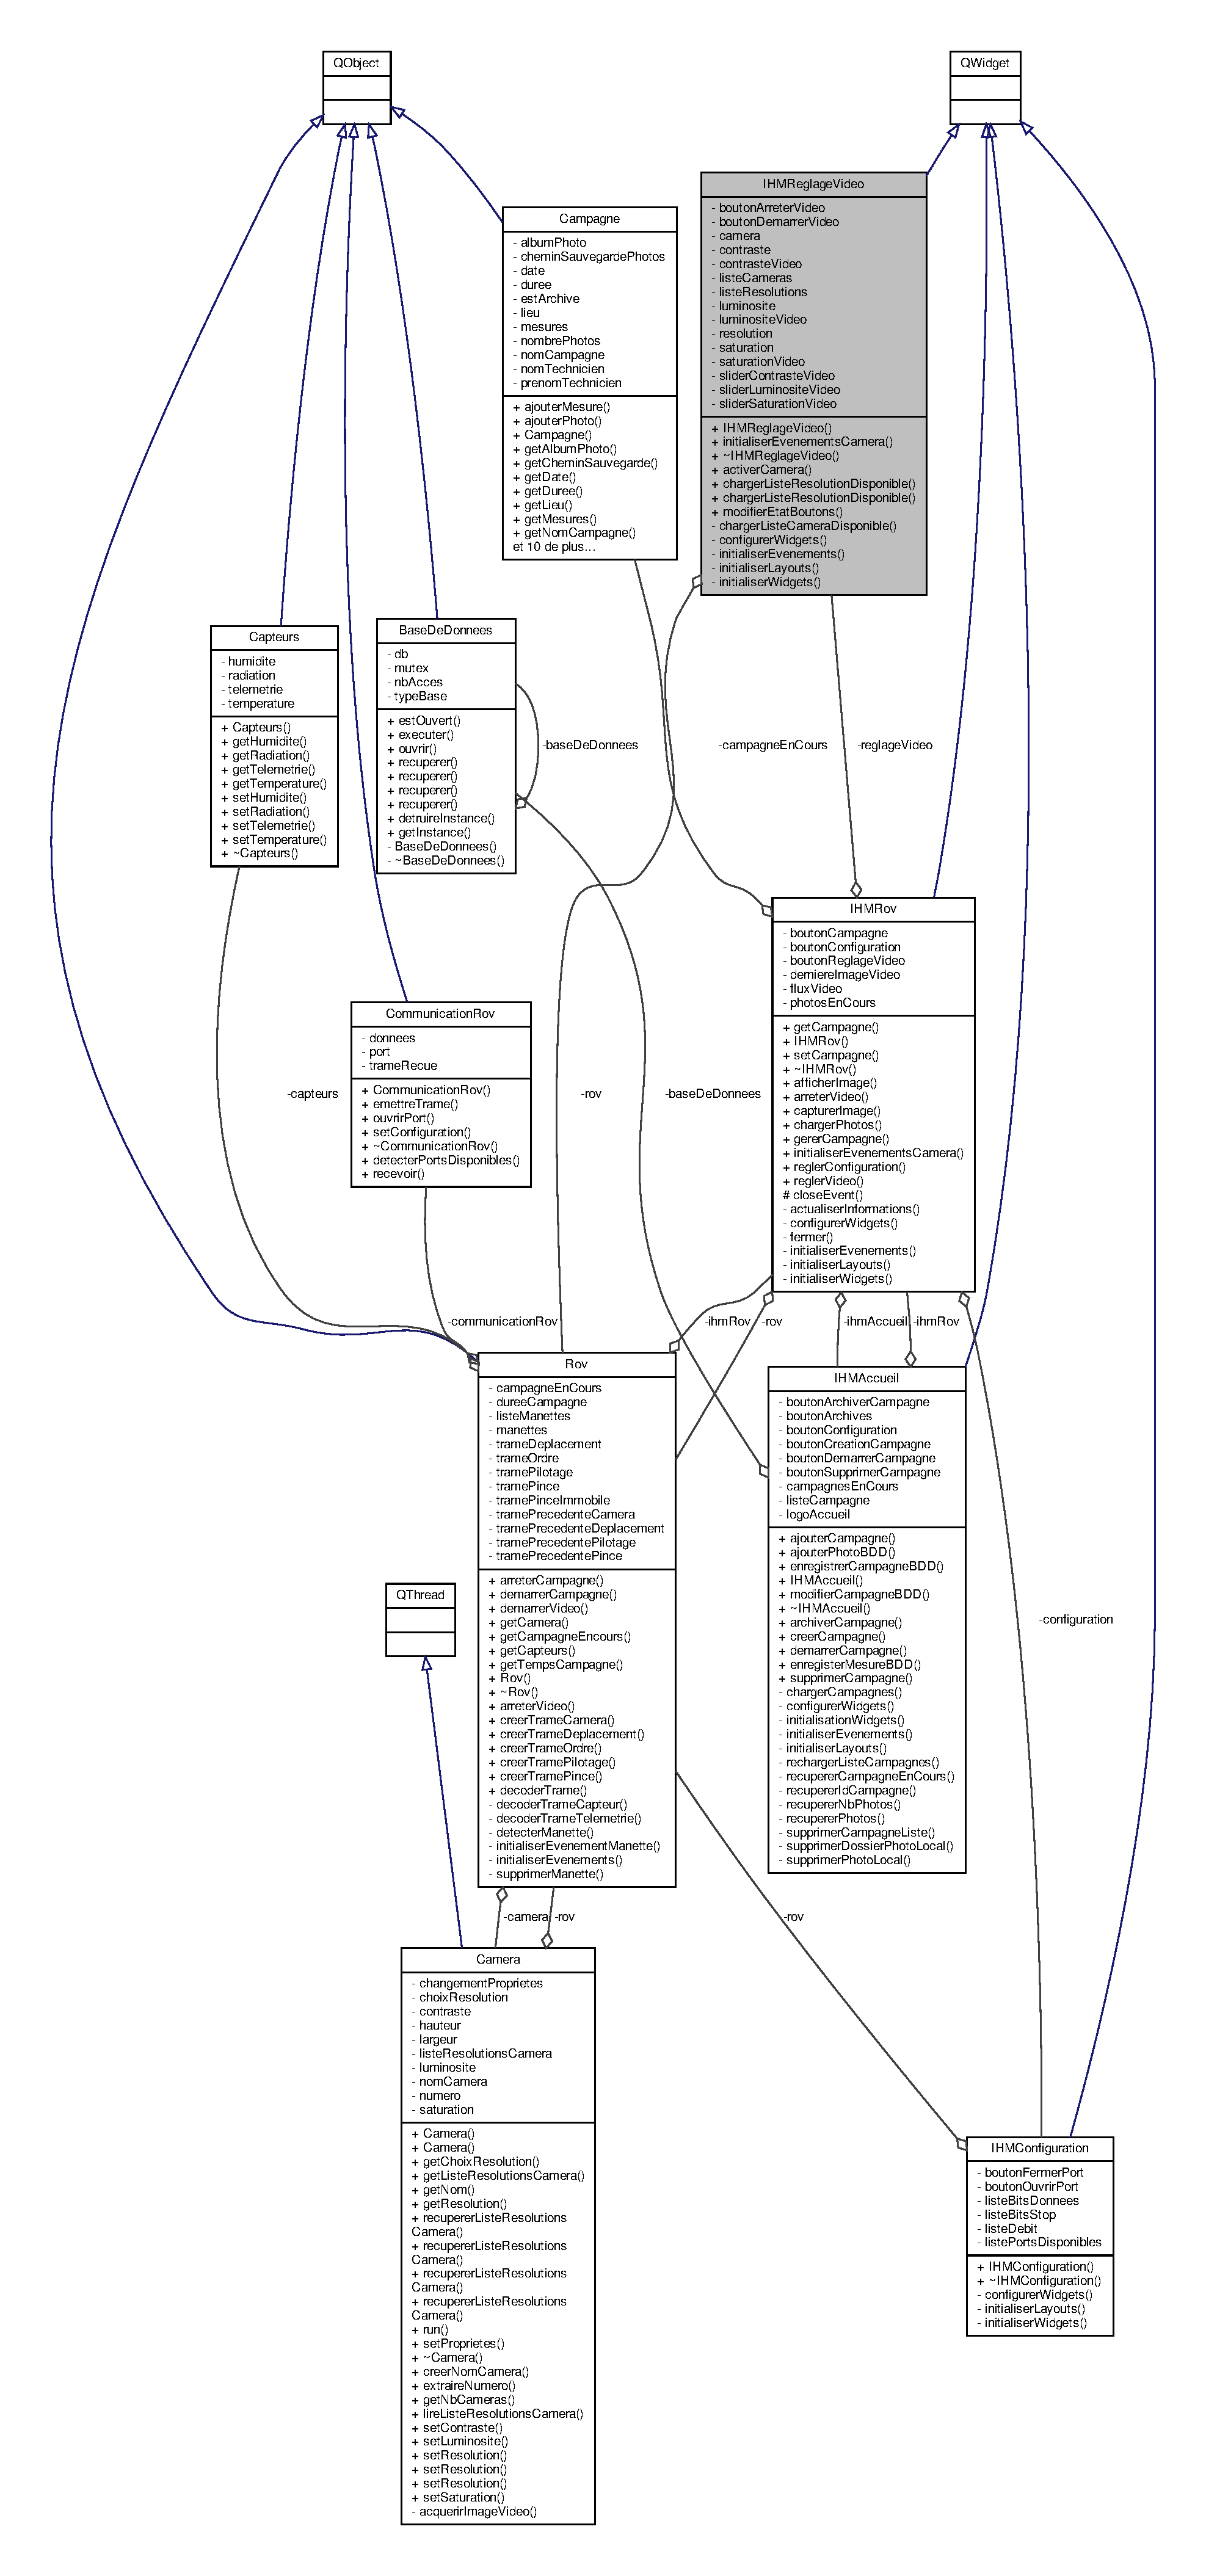
\includegraphics[height=550pt]{class_i_h_m_reglage_video__coll__graph}
\end{center}
\end{figure}
\subsubsection*{Connecteurs publics}
\begin{DoxyCompactItemize}
\item 
void \hyperlink{class_i_h_m_reglage_video_a7e5c5d7515a6c745dfde5c3ad3b61a66}{activer\+Camera} ()
\begin{DoxyCompactList}\small\item\em Active la caméra. \end{DoxyCompactList}\item 
void \hyperlink{class_i_h_m_reglage_video_a26dc15cf9453af24c464f0d6aebb42df}{charger\+Liste\+Resolution\+Disponible} (int index)
\begin{DoxyCompactList}\small\item\em Charge les résolutions pour une caméra sélectionnée. \end{DoxyCompactList}\item 
void \hyperlink{class_i_h_m_reglage_video_a25c0537f7d5b735f80f46f2ae993f424}{charger\+Liste\+Resolution\+Disponible} (Q\+String nom)
\begin{DoxyCompactList}\small\item\em Charge les résolutions pour une caméra sélectionnée. \end{DoxyCompactList}\item 
void \hyperlink{class_i_h_m_reglage_video_ac838581ba03f52e79064cb91ebabb35d}{modifier\+Etat\+Boutons} ()
\begin{DoxyCompactList}\small\item\em Modifie l\textquotesingle{}etat des boutons lors du démarrage du flux vidéo. \end{DoxyCompactList}\end{DoxyCompactItemize}
\subsubsection*{Fonctions membres publiques}
\begin{DoxyCompactItemize}
\item 
\hyperlink{class_i_h_m_reglage_video_aa057ded6ad29a2d7fd117a8e9336c3ad}{I\+H\+M\+Reglage\+Video} (\hyperlink{class_rov}{Rov} $\ast$\hyperlink{class_i_h_m_reglage_video_a755736fe361e651453de6bc21725a626}{rov}, \hyperlink{class_q_widget}{Q\+Widget} $\ast$parent=nullptr)
\begin{DoxyCompactList}\small\item\em Constructeur de la classe Reglage\+Video. \end{DoxyCompactList}\item 
void \hyperlink{class_i_h_m_reglage_video_aba318ba2789177dafcf2651f95603435}{initialiser\+Evenements\+Camera} ()
\begin{DoxyCompactList}\small\item\em Initialise les événements liés à la caméra. \end{DoxyCompactList}\item 
\hyperlink{class_i_h_m_reglage_video_aaf105e0ca892a751632170a3a083dfec}{$\sim$\+I\+H\+M\+Reglage\+Video} ()
\begin{DoxyCompactList}\small\item\em Destructeur de la classe Reglage\+Video. \end{DoxyCompactList}\end{DoxyCompactItemize}
\subsubsection*{Fonctions membres privées}
\begin{DoxyCompactItemize}
\item 
void \hyperlink{class_i_h_m_reglage_video_a0a480faa747bc705b4cf49df4ecc1d44}{charger\+Liste\+Camera\+Disponible} ()
\begin{DoxyCompactList}\small\item\em Charge la liste des caméras disponibles dans la liste déroulante. \end{DoxyCompactList}\item 
void \hyperlink{class_i_h_m_reglage_video_a2e51529e3a822121ae999e13da2180c6}{configurer\+Widgets} ()
\begin{DoxyCompactList}\small\item\em Configure l\textquotesingle{}etat des widgets à la création de l\textquotesingle{}I\+HM. \end{DoxyCompactList}\item 
void \hyperlink{class_i_h_m_reglage_video_a4576b1b6ccfcabf6b2b39d37db2dd248}{initialiser\+Evenements} ()
\begin{DoxyCompactList}\small\item\em Initialise les événements de l\textquotesingle{}I\+HM. \end{DoxyCompactList}\item 
void \hyperlink{class_i_h_m_reglage_video_a6efcf5e8c7dfd272ecb1398985f7332a}{initialiser\+Layouts} ()
\begin{DoxyCompactList}\small\item\em Initialise les layout de l\textquotesingle{}I\+HM. \end{DoxyCompactList}\item 
void \hyperlink{class_i_h_m_reglage_video_ad41172843e79eae9bb64048ec76b81e6}{initialiser\+Widgets} ()
\begin{DoxyCompactList}\small\item\em Initialise les widgets de l\textquotesingle{}I\+HM. \end{DoxyCompactList}\end{DoxyCompactItemize}
\subsubsection*{Attributs privés}
\begin{DoxyCompactItemize}
\item 
Q\+Push\+Button $\ast$ \hyperlink{class_i_h_m_reglage_video_a705db68dd445a91a4144a3c9bf95a9cf}{bouton\+Arreter\+Video}
\begin{DoxyCompactList}\small\item\em Bouton permettant d\textquotesingle{}arrêter le flux vidéo de la caméra selectionner. \end{DoxyCompactList}\item 
Q\+Push\+Button $\ast$ \hyperlink{class_i_h_m_reglage_video_a98d33390551ab92165f192be44f6361d}{bouton\+Demarrer\+Video}
\begin{DoxyCompactList}\small\item\em Bouton permettant de démarrer le flux vidéo de la caméra selectionner. \end{DoxyCompactList}\item 
Q\+Label $\ast$ \hyperlink{class_i_h_m_reglage_video_a5a57047117d423ba8bf62bbcb2baee74}{camera}
\begin{DoxyCompactList}\small\item\em Texte informant de l\textquotesingle{}élément à selectionner (caméra) \end{DoxyCompactList}\item 
Q\+Label $\ast$ \hyperlink{class_i_h_m_reglage_video_ad1aa173a98ced9f3aaeccb0c2712093c}{contraste}
\begin{DoxyCompactList}\small\item\em Texte informant le reglage à modifier. \end{DoxyCompactList}\item 
Q\+Spin\+Box $\ast$ \hyperlink{class_i_h_m_reglage_video_a617e9dbd5a92c35e7e351228354deb63}{contraste\+Video}
\begin{DoxyCompactList}\small\item\em Zone de saisie permettant de modifier le contraste du flux vidéo. \end{DoxyCompactList}\item 
Q\+Combo\+Box $\ast$ \hyperlink{class_i_h_m_reglage_video_a38a35548ddd0e5750917305ac6f32142}{liste\+Cameras}
\begin{DoxyCompactList}\small\item\em Liste déroulante déstiné à accueillir la liste des caméra disponible. \end{DoxyCompactList}\item 
Q\+Combo\+Box $\ast$ \hyperlink{class_i_h_m_reglage_video_ad897355a4350d95f5f219db57ff68d4f}{liste\+Resolutions}
\begin{DoxyCompactList}\small\item\em Liste déroulante déstiné à accueillir la liste des résolutions disponible. \end{DoxyCompactList}\item 
Q\+Label $\ast$ \hyperlink{class_i_h_m_reglage_video_a16b65877af48863d0752e226371952ab}{luminosite}
\begin{DoxyCompactList}\small\item\em Texte informant le reglage à modifier. \end{DoxyCompactList}\item 
Q\+Spin\+Box $\ast$ \hyperlink{class_i_h_m_reglage_video_a9109c0801d582917e78e57c350510ea7}{luminosite\+Video}
\begin{DoxyCompactList}\small\item\em Zone de saisie permettant de modifier la luminosite du flux vidéo. \end{DoxyCompactList}\item 
Q\+Label $\ast$ \hyperlink{class_i_h_m_reglage_video_a7fd79309e9501b8cb340ae61b96c0366}{resolution}
\begin{DoxyCompactList}\small\item\em Texte informant de l\textquotesingle{}élément à selectionner (résolution) \end{DoxyCompactList}\item 
\hyperlink{class_rov}{Rov} $\ast$ \hyperlink{class_i_h_m_reglage_video_a755736fe361e651453de6bc21725a626}{rov}
\begin{DoxyCompactList}\small\item\em Objet rov permettant de mofidier les reglage du flux vidéo. \end{DoxyCompactList}\item 
Q\+Label $\ast$ \hyperlink{class_i_h_m_reglage_video_a452450793da1908cfe89fb9984b914d1}{saturation}
\begin{DoxyCompactList}\small\item\em Texte informant le reglage à modifier. \end{DoxyCompactList}\item 
Q\+Spin\+Box $\ast$ \hyperlink{class_i_h_m_reglage_video_a058bd2a65aefa5f95ff73851f156064c}{saturation\+Video}
\begin{DoxyCompactList}\small\item\em Zone de saisie permettant de modifier la saturation du flux vidéo. \end{DoxyCompactList}\item 
Q\+Slider $\ast$ \hyperlink{class_i_h_m_reglage_video_a69917b4179132a63efe6c3fb63ba666a}{slider\+Contraste\+Video}
\begin{DoxyCompactList}\small\item\em Slider permettant de modifier le contraste du flux vidéo. \end{DoxyCompactList}\item 
Q\+Slider $\ast$ \hyperlink{class_i_h_m_reglage_video_a333b7f1b3239abd5823e0b0f2857716b}{slider\+Luminosite\+Video}
\begin{DoxyCompactList}\small\item\em Slider permettant de modifier la luminosite du flux vidéo. \end{DoxyCompactList}\item 
Q\+Slider $\ast$ \hyperlink{class_i_h_m_reglage_video_aba60de0eccec35f165101b10c0cd33df}{slider\+Saturation\+Video}
\begin{DoxyCompactList}\small\item\em Slider permettant de modifier la saturation du flux vidéo. \end{DoxyCompactList}\end{DoxyCompactItemize}


\subsubsection{Description détaillée}
Classe permettant de regler l\textquotesingle{}affichage du flux video. 

Définition à la ligne \hyperlink{ihmreglagevideo_8h_source_l00023}{23} du fichier \hyperlink{ihmreglagevideo_8h_source}{ihmreglagevideo.\+h}.



\subsubsection{Documentation des constructeurs et destructeur}
\mbox{\Hypertarget{class_i_h_m_reglage_video_aa057ded6ad29a2d7fd117a8e9336c3ad}\label{class_i_h_m_reglage_video_aa057ded6ad29a2d7fd117a8e9336c3ad}} 
\index{I\+H\+M\+Reglage\+Video@{I\+H\+M\+Reglage\+Video}!I\+H\+M\+Reglage\+Video@{I\+H\+M\+Reglage\+Video}}
\index{I\+H\+M\+Reglage\+Video@{I\+H\+M\+Reglage\+Video}!I\+H\+M\+Reglage\+Video@{I\+H\+M\+Reglage\+Video}}
\paragraph{\texorpdfstring{I\+H\+M\+Reglage\+Video()}{IHMReglageVideo()}}
{\footnotesize\ttfamily I\+H\+M\+Reglage\+Video\+::\+I\+H\+M\+Reglage\+Video (\begin{DoxyParamCaption}\item[{\hyperlink{class_rov}{Rov} $\ast$}]{rov,  }\item[{\hyperlink{class_q_widget}{Q\+Widget} $\ast$}]{parent = {\ttfamily nullptr} }\end{DoxyParamCaption})}



Constructeur de la classe Reglage\+Video. 


\begin{DoxyParams}{Paramètres}
{\em rov} & \\
\hline
{\em parent} & \\
\hline
\end{DoxyParams}


Définition à la ligne \hyperlink{ihmreglagevideo_8cpp_source_l00009}{9} du fichier \hyperlink{ihmreglagevideo_8cpp_source}{ihmreglagevideo.\+cpp}.



Références \hyperlink{ihmreglagevideo_8cpp_source_l00047}{configurer\+Widgets()}, \hyperlink{ihmreglagevideo_8cpp_source_l00105}{initialiser\+Evenements()}, \hyperlink{ihmreglagevideo_8cpp_source_l00061}{initialiser\+Layouts()}, et \hyperlink{ihmreglagevideo_8cpp_source_l00023}{initialiser\+Widgets()}.


\begin{DoxyCode}
00009                                                           : \hyperlink{class_q_widget}{QWidget}(parent), 
      \hyperlink{class_i_h_m_reglage_video_a755736fe361e651453de6bc21725a626}{rov}(rov)
00010 \{
00011     qDebug() << Q\_FUNC\_INFO;
00012     \hyperlink{class_i_h_m_reglage_video_ad41172843e79eae9bb64048ec76b81e6}{initialiserWidgets}();
00013     \hyperlink{class_i_h_m_reglage_video_a2e51529e3a822121ae999e13da2180c6}{configurerWidgets}();
00014     \hyperlink{class_i_h_m_reglage_video_a6efcf5e8c7dfd272ecb1398985f7332a}{initialiserLayouts}();
00015     \hyperlink{class_i_h_m_reglage_video_a4576b1b6ccfcabf6b2b39d37db2dd248}{initialiserEvenements}();    
00016 \}
\end{DoxyCode}
\mbox{\Hypertarget{class_i_h_m_reglage_video_aaf105e0ca892a751632170a3a083dfec}\label{class_i_h_m_reglage_video_aaf105e0ca892a751632170a3a083dfec}} 
\index{I\+H\+M\+Reglage\+Video@{I\+H\+M\+Reglage\+Video}!````~I\+H\+M\+Reglage\+Video@{$\sim$\+I\+H\+M\+Reglage\+Video}}
\index{````~I\+H\+M\+Reglage\+Video@{$\sim$\+I\+H\+M\+Reglage\+Video}!I\+H\+M\+Reglage\+Video@{I\+H\+M\+Reglage\+Video}}
\paragraph{\texorpdfstring{$\sim$\+I\+H\+M\+Reglage\+Video()}{~IHMReglageVideo()}}
{\footnotesize\ttfamily I\+H\+M\+Reglage\+Video\+::$\sim$\+I\+H\+M\+Reglage\+Video (\begin{DoxyParamCaption}{ }\end{DoxyParamCaption})}



Destructeur de la classe Reglage\+Video. 



Définition à la ligne \hyperlink{ihmreglagevideo_8cpp_source_l00018}{18} du fichier \hyperlink{ihmreglagevideo_8cpp_source}{ihmreglagevideo.\+cpp}.


\begin{DoxyCode}
00019 \{
00020     qDebug() << Q\_FUNC\_INFO;
00021 \}
\end{DoxyCode}


\subsubsection{Documentation des fonctions membres}
\mbox{\Hypertarget{class_i_h_m_reglage_video_a7e5c5d7515a6c745dfde5c3ad3b61a66}\label{class_i_h_m_reglage_video_a7e5c5d7515a6c745dfde5c3ad3b61a66}} 
\index{I\+H\+M\+Reglage\+Video@{I\+H\+M\+Reglage\+Video}!activer\+Camera@{activer\+Camera}}
\index{activer\+Camera@{activer\+Camera}!I\+H\+M\+Reglage\+Video@{I\+H\+M\+Reglage\+Video}}
\paragraph{\texorpdfstring{activer\+Camera}{activerCamera}}
{\footnotesize\ttfamily void I\+H\+M\+Reglage\+Video\+::activer\+Camera (\begin{DoxyParamCaption}{ }\end{DoxyParamCaption})\hspace{0.3cm}{\ttfamily [slot]}}



Active la caméra. 



Définition à la ligne \hyperlink{ihmreglagevideo_8cpp_source_l00203}{203} du fichier \hyperlink{ihmreglagevideo_8cpp_source}{ihmreglagevideo.\+cpp}.



Références \hyperlink{ihmreglagevideo_8h_source_l00042}{bouton\+Arreter\+Video}, \hyperlink{ihmreglagevideo_8h_source_l00041}{bouton\+Demarrer\+Video}, \hyperlink{rov_8cpp_source_l00161}{Rov\+::demarrer\+Video()}, \hyperlink{ihmreglagevideo_8h_source_l00038}{liste\+Cameras}, \hyperlink{ihmreglagevideo_8h_source_l00040}{liste\+Resolutions}, et \hyperlink{ihmreglagevideo_8h_source_l00027}{rov}.



Référencé par \hyperlink{ihmreglagevideo_8cpp_source_l00105}{initialiser\+Evenements()}.


\begin{DoxyCode}
00204 \{
00205     qDebug() << Q\_FUNC\_INFO << \hyperlink{class_i_h_m_reglage_video_a38a35548ddd0e5750917305ac6f32142}{listeCameras}->currentText() << 
      \hyperlink{class_i_h_m_reglage_video_ad897355a4350d95f5f219db57ff68d4f}{listeResolutions}->currentText() << \hyperlink{class_i_h_m_reglage_video_ad897355a4350d95f5f219db57ff68d4f}{listeResolutions}->currentIndex();
00206     \hyperlink{class_i_h_m_reglage_video_a755736fe361e651453de6bc21725a626}{rov}->\hyperlink{class_rov_aaf1a53557b6e8f0ae2497a0af93bd6db}{demarrerVideo}(\hyperlink{class_i_h_m_reglage_video_a38a35548ddd0e5750917305ac6f32142}{listeCameras}->currentText(), 
      \hyperlink{class_i_h_m_reglage_video_ad897355a4350d95f5f219db57ff68d4f}{listeResolutions}->currentIndex());
00207     \hyperlink{class_i_h_m_reglage_video_a38a35548ddd0e5750917305ac6f32142}{listeCameras}->setEnabled(\textcolor{keyword}{false});
00208     \hyperlink{class_i_h_m_reglage_video_a705db68dd445a91a4144a3c9bf95a9cf}{boutonArreterVideo}->setEnabled(\textcolor{keyword}{true});
00209     \hyperlink{class_i_h_m_reglage_video_a98d33390551ab92165f192be44f6361d}{boutonDemarrerVideo}->setEnabled(\textcolor{keyword}{false});
00210 \}
\end{DoxyCode}
\mbox{\Hypertarget{class_i_h_m_reglage_video_a0a480faa747bc705b4cf49df4ecc1d44}\label{class_i_h_m_reglage_video_a0a480faa747bc705b4cf49df4ecc1d44}} 
\index{I\+H\+M\+Reglage\+Video@{I\+H\+M\+Reglage\+Video}!charger\+Liste\+Camera\+Disponible@{charger\+Liste\+Camera\+Disponible}}
\index{charger\+Liste\+Camera\+Disponible@{charger\+Liste\+Camera\+Disponible}!I\+H\+M\+Reglage\+Video@{I\+H\+M\+Reglage\+Video}}
\paragraph{\texorpdfstring{charger\+Liste\+Camera\+Disponible()}{chargerListeCameraDisponible()}}
{\footnotesize\ttfamily void I\+H\+M\+Reglage\+Video\+::charger\+Liste\+Camera\+Disponible (\begin{DoxyParamCaption}{ }\end{DoxyParamCaption})\hspace{0.3cm}{\ttfamily [private]}}



Charge la liste des caméras disponibles dans la liste déroulante. 



Définition à la ligne \hyperlink{ihmreglagevideo_8cpp_source_l00132}{132} du fichier \hyperlink{ihmreglagevideo_8cpp_source}{ihmreglagevideo.\+cpp}.



Références \hyperlink{ihmreglagevideo_8cpp_source_l00172}{charger\+Liste\+Resolution\+Disponible()}, \hyperlink{rov_8cpp_source_l00144}{Rov\+::get\+Camera()}, \hyperlink{camera_8cpp_source_l00103}{Camera\+::get\+Nom()}, \hyperlink{ihmreglagevideo_8h_source_l00038}{liste\+Cameras}, et \hyperlink{ihmreglagevideo_8h_source_l00027}{rov}.



Référencé par \hyperlink{ihmreglagevideo_8cpp_source_l00117}{initialiser\+Evenements\+Camera()}.


\begin{DoxyCode}
00133 \{
00134     \textcolor{keywordtype}{int} nbCameras = QCameraInfo::availableCameras().count();
00135     qDebug() << Q\_FUNC\_INFO << \textcolor{stringliteral}{"Caméra(s) disponible(s)"} << QCameraInfo::availableCameras().count();    
00136     \textcolor{keywordflow}{if} (nbCameras > 0)
00137     \{
00138 \textcolor{preprocessor}{       #ifndef SANS\_DETECTION}
00139        QList<QCameraInfo> cameras = QCameraInfo::availableCameras();
00140        \hyperlink{class_i_h_m_reglage_video_a38a35548ddd0e5750917305ac6f32142}{listeCameras}->clear();
00141        \textcolor{keywordtype}{int} choix = -1, i = 0;
00142        \textcolor{keywordflow}{foreach} (\textcolor{keyword}{const} QCameraInfo &cameraInfo, cameras)
00143        \{
00144            \hyperlink{class_i_h_m_reglage_video_a38a35548ddd0e5750917305ac6f32142}{listeCameras}->addItem(cameraInfo.deviceName());
00145            qDebug() << Q\_FUNC\_INFO << \textcolor{stringliteral}{"Device"} << cameraInfo.deviceName();
00146            qDebug() << Q\_FUNC\_INFO << \textcolor{stringliteral}{"Description"} << cameraInfo.description();
00147            \textcolor{keywordflow}{if}(\hyperlink{class_i_h_m_reglage_video_a755736fe361e651453de6bc21725a626}{rov}->\hyperlink{class_rov_ac1eeb568d39018359b89384c2ee6ee86}{getCamera}() != \textcolor{keyword}{nullptr})
00148            \{
00149                \textcolor{keywordflow}{if}(cameraInfo.deviceName() == \hyperlink{class_i_h_m_reglage_video_a755736fe361e651453de6bc21725a626}{rov}->\hyperlink{class_rov_ac1eeb568d39018359b89384c2ee6ee86}{getCamera}()->
      \hyperlink{class_camera_a9b27a8a444006f40548a9a4ecf4d7256}{getNom}())
00150                \{
00151                    choix = i;
00152                \}
00153            \}
00154            i++;
00155        \}
00156 \textcolor{preprocessor}{       #else}
00157        \textcolor{keywordtype}{int} choix = 0;
00158        qDebug() << Q\_FUNC\_INFO << \textcolor{stringliteral}{"Device"} << \hyperlink{class_i_h_m_reglage_video_a755736fe361e651453de6bc21725a626}{rov}->\hyperlink{class_rov_ac1eeb568d39018359b89384c2ee6ee86}{getCamera}()->
      \hyperlink{class_camera_a9b27a8a444006f40548a9a4ecf4d7256}{getNom}();
00159        \hyperlink{class_i_h_m_reglage_video_a38a35548ddd0e5750917305ac6f32142}{listeCameras}->addItem(\hyperlink{class_i_h_m_reglage_video_a755736fe361e651453de6bc21725a626}{rov}->\hyperlink{class_rov_ac1eeb568d39018359b89384c2ee6ee86}{getCamera}()->\hyperlink{class_camera_a9b27a8a444006f40548a9a4ecf4d7256}{getNom}());
00160 \textcolor{preprocessor}{       #endif}
00161 
00162        \textcolor{keywordflow}{if}(choix != -1)
00163        \{
00164            \textcolor{keywordflow}{if}(\hyperlink{class_i_h_m_reglage_video_a755736fe361e651453de6bc21725a626}{rov}->\hyperlink{class_rov_ac1eeb568d39018359b89384c2ee6ee86}{getCamera}() != \textcolor{keyword}{nullptr})
00165                 \hyperlink{class_i_h_m_reglage_video_a26dc15cf9453af24c464f0d6aebb42df}{chargerListeResolutionDisponible}(
      \hyperlink{class_i_h_m_reglage_video_a755736fe361e651453de6bc21725a626}{rov}->\hyperlink{class_rov_ac1eeb568d39018359b89384c2ee6ee86}{getCamera}()->\hyperlink{class_camera_a9b27a8a444006f40548a9a4ecf4d7256}{getNom}());
00166            \hyperlink{class_i_h_m_reglage_video_a38a35548ddd0e5750917305ac6f32142}{listeCameras}->setCurrentIndex(choix);
00167        \}       
00168     \}
00169 
00170 \}
\end{DoxyCode}
\mbox{\Hypertarget{class_i_h_m_reglage_video_a26dc15cf9453af24c464f0d6aebb42df}\label{class_i_h_m_reglage_video_a26dc15cf9453af24c464f0d6aebb42df}} 
\index{I\+H\+M\+Reglage\+Video@{I\+H\+M\+Reglage\+Video}!charger\+Liste\+Resolution\+Disponible@{charger\+Liste\+Resolution\+Disponible}}
\index{charger\+Liste\+Resolution\+Disponible@{charger\+Liste\+Resolution\+Disponible}!I\+H\+M\+Reglage\+Video@{I\+H\+M\+Reglage\+Video}}
\paragraph{\texorpdfstring{charger\+Liste\+Resolution\+Disponible}{chargerListeResolutionDisponible}\hspace{0.1cm}{\footnotesize\ttfamily [1/2]}}
{\footnotesize\ttfamily void I\+H\+M\+Reglage\+Video\+::charger\+Liste\+Resolution\+Disponible (\begin{DoxyParamCaption}\item[{int}]{index }\end{DoxyParamCaption})\hspace{0.3cm}{\ttfamily [slot]}}



Charge les résolutions pour une caméra sélectionnée. 


\begin{DoxyParams}{Paramètres}
{\em index} & \\
\hline
\end{DoxyParams}


Définition à la ligne \hyperlink{ihmreglagevideo_8cpp_source_l00172}{172} du fichier \hyperlink{ihmreglagevideo_8cpp_source}{ihmreglagevideo.\+cpp}.



Références \hyperlink{ihmreglagevideo_8h_source_l00038}{liste\+Cameras}.



Référencé par \hyperlink{ihmreglagevideo_8cpp_source_l00132}{charger\+Liste\+Camera\+Disponible()}, \hyperlink{ihmreglagevideo_8cpp_source_l00117}{initialiser\+Evenements\+Camera()}, et \hyperlink{ihmreglagevideo_8cpp_source_l00212}{modifier\+Etat\+Boutons()}.


\begin{DoxyCode}
00173 \{
00174     \textcolor{keywordflow}{if}(index < 0)
00175         \textcolor{keywordflow}{return};
00176     \hyperlink{class_i_h_m_reglage_video_a26dc15cf9453af24c464f0d6aebb42df}{chargerListeResolutionDisponible}(
      \hyperlink{class_i_h_m_reglage_video_a38a35548ddd0e5750917305ac6f32142}{listeCameras}->currentText());
00177 \}
\end{DoxyCode}
\mbox{\Hypertarget{class_i_h_m_reglage_video_a25c0537f7d5b735f80f46f2ae993f424}\label{class_i_h_m_reglage_video_a25c0537f7d5b735f80f46f2ae993f424}} 
\index{I\+H\+M\+Reglage\+Video@{I\+H\+M\+Reglage\+Video}!charger\+Liste\+Resolution\+Disponible@{charger\+Liste\+Resolution\+Disponible}}
\index{charger\+Liste\+Resolution\+Disponible@{charger\+Liste\+Resolution\+Disponible}!I\+H\+M\+Reglage\+Video@{I\+H\+M\+Reglage\+Video}}
\paragraph{\texorpdfstring{charger\+Liste\+Resolution\+Disponible}{chargerListeResolutionDisponible}\hspace{0.1cm}{\footnotesize\ttfamily [2/2]}}
{\footnotesize\ttfamily void I\+H\+M\+Reglage\+Video\+::charger\+Liste\+Resolution\+Disponible (\begin{DoxyParamCaption}\item[{Q\+String}]{nom }\end{DoxyParamCaption})\hspace{0.3cm}{\ttfamily [slot]}}



Charge les résolutions pour une caméra sélectionnée. 


\begin{DoxyParams}{Paramètres}
{\em nom} & \\
\hline
\end{DoxyParams}


Définition à la ligne \hyperlink{ihmreglagevideo_8cpp_source_l00179}{179} du fichier \hyperlink{ihmreglagevideo_8cpp_source}{ihmreglagevideo.\+cpp}.



Références \hyperlink{rov_8cpp_source_l00144}{Rov\+::get\+Camera()}, \hyperlink{camera_8cpp_source_l00128}{Camera\+::get\+Choix\+Resolution()}, \hyperlink{camera_8cpp_source_l00121}{Camera\+::get\+Resolution()}, \hyperlink{camera_8cpp_source_l00304}{Camera\+::lire\+Liste\+Resolutions\+Camera()}, \hyperlink{ihmreglagevideo_8h_source_l00040}{liste\+Resolutions}, \hyperlink{ihmreglagevideo_8h_source_l00039}{resolution}, et \hyperlink{ihmreglagevideo_8h_source_l00027}{rov}.


\begin{DoxyCode}
00180 \{
00181 \textcolor{preprocessor}{    #ifndef SANS\_DETECTION}
00182     QCameraInfo cameraInfo(nom.toLatin1());
00183     QList<QSize> liste = \hyperlink{class_camera_ac4756add4cb6bef60e38f3da79c2383f}{Camera::lireListeResolutionsCamera}(cameraInfo);
00184     \hyperlink{class_i_h_m_reglage_video_ad897355a4350d95f5f219db57ff68d4f}{listeResolutions}->clear();
00185     \textcolor{keywordflow}{foreach} (\textcolor{keyword}{const} QSize &\hyperlink{class_i_h_m_reglage_video_a7fd79309e9501b8cb340ae61b96c0366}{resolution}, liste)
00186     \{
00187         qDebug() << Q\_FUNC\_INFO << resolution.width() << \textcolor{stringliteral}{"x"} << resolution.height();
00188         \hyperlink{class_i_h_m_reglage_video_ad897355a4350d95f5f219db57ff68d4f}{listeResolutions}->addItem(QString::number(resolution.width()) + QString(\textcolor{stringliteral}{"x"}) + 
      QString::number(resolution.height()));
00189     \}
00190 \textcolor{preprocessor}{    #else}
00191     \hyperlink{class_i_h_m_reglage_video_ad897355a4350d95f5f219db57ff68d4f}{listeResolutions}->clear();
00192     QSize resolutionDefaut = \hyperlink{class_i_h_m_reglage_video_a755736fe361e651453de6bc21725a626}{rov}->\hyperlink{class_rov_ac1eeb568d39018359b89384c2ee6ee86}{getCamera}()->\hyperlink{class_camera_a9fae9d9b6fa352ff96c9874d9b085454}{getResolution}();
00193     qDebug() << Q\_FUNC\_INFO << resolutionDefaut.width() << \textcolor{stringliteral}{"x"} << resolutionDefaut.height();
00194     \hyperlink{class_i_h_m_reglage_video_ad897355a4350d95f5f219db57ff68d4f}{listeResolutions}->addItem(QString::number(resolutionDefaut.width()) + QString(\textcolor{stringliteral}{"x"}) + 
      QString::number(resolutionDefaut.height()));
00195 \textcolor{preprocessor}{    #endif}
00196     \textcolor{keywordflow}{if}(\hyperlink{class_i_h_m_reglage_video_a755736fe361e651453de6bc21725a626}{rov}->\hyperlink{class_rov_ac1eeb568d39018359b89384c2ee6ee86}{getCamera}() != \textcolor{keyword}{nullptr})
00197     \{
00198         qDebug() << Q\_FUNC\_INFO << \textcolor{stringliteral}{"choixResolution"} << \hyperlink{class_i_h_m_reglage_video_a755736fe361e651453de6bc21725a626}{rov}->\hyperlink{class_rov_ac1eeb568d39018359b89384c2ee6ee86}{getCamera}()->
      \hyperlink{class_camera_ab9f05b05c29416dce6471b5a03db98ea}{getChoixResolution}();
00199         \hyperlink{class_i_h_m_reglage_video_ad897355a4350d95f5f219db57ff68d4f}{listeResolutions}->setCurrentIndex(\hyperlink{class_i_h_m_reglage_video_a755736fe361e651453de6bc21725a626}{rov}->\hyperlink{class_rov_ac1eeb568d39018359b89384c2ee6ee86}{getCamera}()->
      \hyperlink{class_camera_ab9f05b05c29416dce6471b5a03db98ea}{getChoixResolution}());
00200     \}
00201 \}
\end{DoxyCode}
\mbox{\Hypertarget{class_i_h_m_reglage_video_a2e51529e3a822121ae999e13da2180c6}\label{class_i_h_m_reglage_video_a2e51529e3a822121ae999e13da2180c6}} 
\index{I\+H\+M\+Reglage\+Video@{I\+H\+M\+Reglage\+Video}!configurer\+Widgets@{configurer\+Widgets}}
\index{configurer\+Widgets@{configurer\+Widgets}!I\+H\+M\+Reglage\+Video@{I\+H\+M\+Reglage\+Video}}
\paragraph{\texorpdfstring{configurer\+Widgets()}{configurerWidgets()}}
{\footnotesize\ttfamily void I\+H\+M\+Reglage\+Video\+::configurer\+Widgets (\begin{DoxyParamCaption}{ }\end{DoxyParamCaption})\hspace{0.3cm}{\ttfamily [private]}}



Configure l\textquotesingle{}etat des widgets à la création de l\textquotesingle{}I\+HM. 



Définition à la ligne \hyperlink{ihmreglagevideo_8cpp_source_l00047}{47} du fichier \hyperlink{ihmreglagevideo_8cpp_source}{ihmreglagevideo.\+cpp}.



Références \hyperlink{ihmreglagevideo_8h_source_l00041}{bouton\+Demarrer\+Video}, \hyperlink{ihmreglagevideo_8h_source_l00035}{contraste\+Video}, \hyperlink{ihmreglagevideo_8h_source_l00038}{liste\+Cameras}, \hyperlink{ihmreglagevideo_8h_source_l00034}{luminosite\+Video}, \hyperlink{ihmreglagevideo_8h_source_l00036}{saturation\+Video}, \hyperlink{ihmreglagevideo_8h_source_l00029}{slider\+Contraste\+Video}, \hyperlink{ihmreglagevideo_8h_source_l00028}{slider\+Luminosite\+Video}, et \hyperlink{ihmreglagevideo_8h_source_l00030}{slider\+Saturation\+Video}.



Référencé par \hyperlink{ihmreglagevideo_8cpp_source_l00009}{I\+H\+M\+Reglage\+Video()}.


\begin{DoxyCode}
00048 \{
00049     \hyperlink{class_i_h_m_reglage_video_a333b7f1b3239abd5823e0b0f2857716b}{sliderLuminositeVideo}->setValue(50);
00050     \hyperlink{class_i_h_m_reglage_video_a69917b4179132a63efe6c3fb63ba666a}{sliderContrasteVideo}->setValue(50);
00051     \hyperlink{class_i_h_m_reglage_video_aba60de0eccec35f165101b10c0cd33df}{sliderSaturationVideo}->setValue(50);
00052 
00053     \hyperlink{class_i_h_m_reglage_video_a9109c0801d582917e78e57c350510ea7}{luminositeVideo}->setValue(50);
00054     \hyperlink{class_i_h_m_reglage_video_a617e9dbd5a92c35e7e351228354deb63}{contrasteVideo}->setValue(50);
00055     \hyperlink{class_i_h_m_reglage_video_a058bd2a65aefa5f95ff73851f156064c}{saturationVideo}->setValue(50);
00056 
00057     \hyperlink{class_i_h_m_reglage_video_a98d33390551ab92165f192be44f6361d}{boutonDemarrerVideo}->setEnabled(\textcolor{keyword}{false});
00058     \hyperlink{class_i_h_m_reglage_video_a38a35548ddd0e5750917305ac6f32142}{listeCameras}->setEnabled(\textcolor{keyword}{false});
00059 \}
\end{DoxyCode}
\mbox{\Hypertarget{class_i_h_m_reglage_video_a4576b1b6ccfcabf6b2b39d37db2dd248}\label{class_i_h_m_reglage_video_a4576b1b6ccfcabf6b2b39d37db2dd248}} 
\index{I\+H\+M\+Reglage\+Video@{I\+H\+M\+Reglage\+Video}!initialiser\+Evenements@{initialiser\+Evenements}}
\index{initialiser\+Evenements@{initialiser\+Evenements}!I\+H\+M\+Reglage\+Video@{I\+H\+M\+Reglage\+Video}}
\paragraph{\texorpdfstring{initialiser\+Evenements()}{initialiserEvenements()}}
{\footnotesize\ttfamily void I\+H\+M\+Reglage\+Video\+::initialiser\+Evenements (\begin{DoxyParamCaption}{ }\end{DoxyParamCaption})\hspace{0.3cm}{\ttfamily [private]}}



Initialise les événements de l\textquotesingle{}I\+HM. 



Définition à la ligne \hyperlink{ihmreglagevideo_8cpp_source_l00105}{105} du fichier \hyperlink{ihmreglagevideo_8cpp_source}{ihmreglagevideo.\+cpp}.



Références \hyperlink{ihmreglagevideo_8cpp_source_l00203}{activer\+Camera()}, \hyperlink{ihmreglagevideo_8h_source_l00042}{bouton\+Arreter\+Video}, \hyperlink{ihmreglagevideo_8h_source_l00041}{bouton\+Demarrer\+Video}, \hyperlink{ihmreglagevideo_8h_source_l00035}{contraste\+Video}, \hyperlink{ihmreglagevideo_8h_source_l00034}{luminosite\+Video}, \hyperlink{ihmreglagevideo_8h_source_l00027}{rov}, \hyperlink{ihmreglagevideo_8h_source_l00036}{saturation\+Video}, \hyperlink{ihmreglagevideo_8h_source_l00029}{slider\+Contraste\+Video}, \hyperlink{ihmreglagevideo_8h_source_l00028}{slider\+Luminosite\+Video}, et \hyperlink{ihmreglagevideo_8h_source_l00030}{slider\+Saturation\+Video}.



Référencé par \hyperlink{ihmreglagevideo_8cpp_source_l00009}{I\+H\+M\+Reglage\+Video()}.


\begin{DoxyCode}
00106 \{
00107     connect(\hyperlink{class_i_h_m_reglage_video_a333b7f1b3239abd5823e0b0f2857716b}{sliderLuminositeVideo}, SIGNAL(valueChanged(\textcolor{keywordtype}{int})), 
      \hyperlink{class_i_h_m_reglage_video_a9109c0801d582917e78e57c350510ea7}{luminositeVideo}, SLOT(setValue(\textcolor{keywordtype}{int})));
00108     connect(\hyperlink{class_i_h_m_reglage_video_a69917b4179132a63efe6c3fb63ba666a}{sliderContrasteVideo}, SIGNAL(valueChanged(\textcolor{keywordtype}{int})), 
      \hyperlink{class_i_h_m_reglage_video_a617e9dbd5a92c35e7e351228354deb63}{contrasteVideo}, SLOT(setValue(\textcolor{keywordtype}{int})));
00109     connect(\hyperlink{class_i_h_m_reglage_video_aba60de0eccec35f165101b10c0cd33df}{sliderSaturationVideo}, SIGNAL(valueChanged(\textcolor{keywordtype}{int})), 
      \hyperlink{class_i_h_m_reglage_video_a058bd2a65aefa5f95ff73851f156064c}{saturationVideo}, SLOT(setValue(\textcolor{keywordtype}{int})));
00110     connect(\hyperlink{class_i_h_m_reglage_video_a9109c0801d582917e78e57c350510ea7}{luminositeVideo}, SIGNAL(valueChanged(\textcolor{keywordtype}{int})), 
      \hyperlink{class_i_h_m_reglage_video_a333b7f1b3239abd5823e0b0f2857716b}{sliderLuminositeVideo}, SLOT(setValue(\textcolor{keywordtype}{int})));
00111     connect(\hyperlink{class_i_h_m_reglage_video_a617e9dbd5a92c35e7e351228354deb63}{contrasteVideo}, SIGNAL(valueChanged(\textcolor{keywordtype}{int})), 
      \hyperlink{class_i_h_m_reglage_video_a69917b4179132a63efe6c3fb63ba666a}{sliderContrasteVideo}, SLOT(setValue(\textcolor{keywordtype}{int})));
00112     connect(\hyperlink{class_i_h_m_reglage_video_a058bd2a65aefa5f95ff73851f156064c}{saturationVideo}, SIGNAL(valueChanged(\textcolor{keywordtype}{int})), 
      \hyperlink{class_i_h_m_reglage_video_aba60de0eccec35f165101b10c0cd33df}{sliderSaturationVideo}, SLOT(setValue(\textcolor{keywordtype}{int})));
00113     connect(\hyperlink{class_i_h_m_reglage_video_a705db68dd445a91a4144a3c9bf95a9cf}{boutonArreterVideo}, SIGNAL(clicked()), \hyperlink{class_i_h_m_reglage_video_a755736fe361e651453de6bc21725a626}{rov}, SLOT(arreterVideo()));
00114     connect(\hyperlink{class_i_h_m_reglage_video_a98d33390551ab92165f192be44f6361d}{boutonDemarrerVideo}, SIGNAL(clicked()), \textcolor{keyword}{this}, SLOT(
      \hyperlink{class_i_h_m_reglage_video_a7e5c5d7515a6c745dfde5c3ad3b61a66}{activerCamera}()));
00115 \}
\end{DoxyCode}
\mbox{\Hypertarget{class_i_h_m_reglage_video_aba318ba2789177dafcf2651f95603435}\label{class_i_h_m_reglage_video_aba318ba2789177dafcf2651f95603435}} 
\index{I\+H\+M\+Reglage\+Video@{I\+H\+M\+Reglage\+Video}!initialiser\+Evenements\+Camera@{initialiser\+Evenements\+Camera}}
\index{initialiser\+Evenements\+Camera@{initialiser\+Evenements\+Camera}!I\+H\+M\+Reglage\+Video@{I\+H\+M\+Reglage\+Video}}
\paragraph{\texorpdfstring{initialiser\+Evenements\+Camera()}{initialiserEvenementsCamera()}}
{\footnotesize\ttfamily void I\+H\+M\+Reglage\+Video\+::initialiser\+Evenements\+Camera (\begin{DoxyParamCaption}{ }\end{DoxyParamCaption})}



Initialise les événements liés à la caméra. 



Définition à la ligne \hyperlink{ihmreglagevideo_8cpp_source_l00117}{117} du fichier \hyperlink{ihmreglagevideo_8cpp_source}{ihmreglagevideo.\+cpp}.



Références \hyperlink{ihmreglagevideo_8cpp_source_l00132}{charger\+Liste\+Camera\+Disponible()}, \hyperlink{ihmreglagevideo_8cpp_source_l00172}{charger\+Liste\+Resolution\+Disponible()}, \hyperlink{ihmreglagevideo_8h_source_l00035}{contraste\+Video}, \hyperlink{rov_8cpp_source_l00144}{Rov\+::get\+Camera()}, \hyperlink{ihmreglagevideo_8h_source_l00038}{liste\+Cameras}, \hyperlink{ihmreglagevideo_8h_source_l00040}{liste\+Resolutions}, \hyperlink{ihmreglagevideo_8h_source_l00034}{luminosite\+Video}, \hyperlink{ihmreglagevideo_8h_source_l00027}{rov}, et \hyperlink{ihmreglagevideo_8h_source_l00036}{saturation\+Video}.



Référencé par \hyperlink{ihmrov_8cpp_source_l00229}{I\+H\+M\+Rov\+::initialiser\+Evenements\+Camera()}.


\begin{DoxyCode}
00118 \{
00119     \textcolor{keywordflow}{if}(\hyperlink{class_i_h_m_reglage_video_a755736fe361e651453de6bc21725a626}{rov}->\hyperlink{class_rov_ac1eeb568d39018359b89384c2ee6ee86}{getCamera}() != \textcolor{keyword}{nullptr})
00120     \{
00121         \textcolor{keywordflow}{if}(\hyperlink{class_i_h_m_reglage_video_a755736fe361e651453de6bc21725a626}{rov}->\hyperlink{class_rov_ac1eeb568d39018359b89384c2ee6ee86}{getCamera}()->isRunning())
00122             \textcolor{keywordflow}{return};
00123         \hyperlink{class_i_h_m_reglage_video_a0a480faa747bc705b4cf49df4ecc1d44}{chargerListeCameraDisponible}();
00124         connect(\hyperlink{class_i_h_m_reglage_video_a9109c0801d582917e78e57c350510ea7}{luminositeVideo}, SIGNAL(valueChanged(\textcolor{keywordtype}{int})), \hyperlink{class_i_h_m_reglage_video_a755736fe361e651453de6bc21725a626}{rov}->
      \hyperlink{class_rov_ac1eeb568d39018359b89384c2ee6ee86}{getCamera}(), SLOT(setLuminosite(\textcolor{keywordtype}{int})));
00125         connect(\hyperlink{class_i_h_m_reglage_video_a617e9dbd5a92c35e7e351228354deb63}{contrasteVideo}, SIGNAL(valueChanged(\textcolor{keywordtype}{int})), \hyperlink{class_i_h_m_reglage_video_a755736fe361e651453de6bc21725a626}{rov}->
      \hyperlink{class_rov_ac1eeb568d39018359b89384c2ee6ee86}{getCamera}(), SLOT(setContraste(\textcolor{keywordtype}{int})));
00126         connect(\hyperlink{class_i_h_m_reglage_video_a058bd2a65aefa5f95ff73851f156064c}{saturationVideo}, SIGNAL(valueChanged(\textcolor{keywordtype}{int})), \hyperlink{class_i_h_m_reglage_video_a755736fe361e651453de6bc21725a626}{rov}->
      \hyperlink{class_rov_ac1eeb568d39018359b89384c2ee6ee86}{getCamera}(), SLOT(setSaturation(\textcolor{keywordtype}{int})));
00127         connect(\hyperlink{class_i_h_m_reglage_video_a38a35548ddd0e5750917305ac6f32142}{listeCameras}, SIGNAL(currentIndexChanged(\textcolor{keywordtype}{int})), \textcolor{keyword}{this}, SLOT(
      \hyperlink{class_i_h_m_reglage_video_a26dc15cf9453af24c464f0d6aebb42df}{chargerListeResolutionDisponible}(\textcolor{keywordtype}{int})));
00128         connect(\hyperlink{class_i_h_m_reglage_video_ad897355a4350d95f5f219db57ff68d4f}{listeResolutions}, SIGNAL(currentIndexChanged(\textcolor{keywordtype}{int})), 
      \hyperlink{class_i_h_m_reglage_video_a755736fe361e651453de6bc21725a626}{rov}->\hyperlink{class_rov_ac1eeb568d39018359b89384c2ee6ee86}{getCamera}(), SLOT(setResolution(\textcolor{keywordtype}{int})));
00129     \}
00130 \}
\end{DoxyCode}
\mbox{\Hypertarget{class_i_h_m_reglage_video_a6efcf5e8c7dfd272ecb1398985f7332a}\label{class_i_h_m_reglage_video_a6efcf5e8c7dfd272ecb1398985f7332a}} 
\index{I\+H\+M\+Reglage\+Video@{I\+H\+M\+Reglage\+Video}!initialiser\+Layouts@{initialiser\+Layouts}}
\index{initialiser\+Layouts@{initialiser\+Layouts}!I\+H\+M\+Reglage\+Video@{I\+H\+M\+Reglage\+Video}}
\paragraph{\texorpdfstring{initialiser\+Layouts()}{initialiserLayouts()}}
{\footnotesize\ttfamily void I\+H\+M\+Reglage\+Video\+::initialiser\+Layouts (\begin{DoxyParamCaption}{ }\end{DoxyParamCaption})\hspace{0.3cm}{\ttfamily [private]}}



Initialise les layout de l\textquotesingle{}I\+HM. 



Définition à la ligne \hyperlink{ihmreglagevideo_8cpp_source_l00061}{61} du fichier \hyperlink{ihmreglagevideo_8cpp_source}{ihmreglagevideo.\+cpp}.



Références \hyperlink{ihmreglagevideo_8h_source_l00042}{bouton\+Arreter\+Video}, \hyperlink{ihmreglagevideo_8h_source_l00041}{bouton\+Demarrer\+Video}, \hyperlink{ihmreglagevideo_8h_source_l00037}{camera}, \hyperlink{ihmreglagevideo_8h_source_l00032}{contraste}, \hyperlink{ihmreglagevideo_8h_source_l00035}{contraste\+Video}, \hyperlink{ihmreglagevideo_8h_source_l00038}{liste\+Cameras}, \hyperlink{ihmreglagevideo_8h_source_l00040}{liste\+Resolutions}, \hyperlink{ihmreglagevideo_8h_source_l00031}{luminosite}, \hyperlink{ihmreglagevideo_8h_source_l00034}{luminosite\+Video}, \hyperlink{ihmreglagevideo_8h_source_l00014}{N\+O\+M\+\_\+\+F\+E\+N\+E\+T\+R\+E\+\_\+\+R\+E\+G\+L\+A\+G\+E\+V\+I\+D\+EO}, \hyperlink{ihmreglagevideo_8h_source_l00039}{resolution}, \hyperlink{ihmreglagevideo_8h_source_l00033}{saturation}, \hyperlink{ihmreglagevideo_8h_source_l00036}{saturation\+Video}, \hyperlink{ihmreglagevideo_8h_source_l00029}{slider\+Contraste\+Video}, \hyperlink{ihmreglagevideo_8h_source_l00028}{slider\+Luminosite\+Video}, et \hyperlink{ihmreglagevideo_8h_source_l00030}{slider\+Saturation\+Video}.



Référencé par \hyperlink{ihmreglagevideo_8cpp_source_l00009}{I\+H\+M\+Reglage\+Video()}.


\begin{DoxyCode}
00062 \{
00063     QVBoxLayout *layoutPrincipal = \textcolor{keyword}{new} QVBoxLayout;
00064     QHBoxLayout *layoutReglageVideo = \textcolor{keyword}{new} QHBoxLayout;
00065     QVBoxLayout *layoutConfigurationLuminosite = \textcolor{keyword}{new} QVBoxLayout;
00066     QVBoxLayout *layoutConfigurationContraste = \textcolor{keyword}{new} QVBoxLayout;
00067     QVBoxLayout *layoutConfigurationSaturation = \textcolor{keyword}{new} QVBoxLayout;
00068     QHBoxLayout *layoutCamera = \textcolor{keyword}{new} QHBoxLayout;
00069     QHBoxLayout *layoutBoutonCamera = \textcolor{keyword}{new} QHBoxLayout;
00070 
00071     layoutReglageVideo->setAlignment(Qt::AlignLeft);
00072     layoutConfigurationContraste->setAlignment(Qt::AlignTop);
00073     layoutConfigurationLuminosite->setAlignment(Qt::AlignTop);
00074     layoutConfigurationSaturation->setAlignment(Qt::AlignTop);
00075     layoutBoutonCamera->setAlignment(Qt::AlignLeft);
00076 
00077     layoutPrincipal->addLayout(layoutReglageVideo);
00078     layoutPrincipal->addLayout(layoutCamera);
00079     layoutPrincipal->addLayout(layoutBoutonCamera);
00080 
00081     layoutReglageVideo->addLayout(layoutConfigurationLuminosite);
00082     layoutReglageVideo->addLayout(layoutConfigurationContraste);
00083     layoutReglageVideo->addLayout(layoutConfigurationSaturation);
00084 
00085     layoutConfigurationLuminosite->addWidget(\hyperlink{class_i_h_m_reglage_video_a16b65877af48863d0752e226371952ab}{luminosite});
00086     layoutConfigurationLuminosite->addWidget(\hyperlink{class_i_h_m_reglage_video_a333b7f1b3239abd5823e0b0f2857716b}{sliderLuminositeVideo});
00087     layoutConfigurationLuminosite->addWidget(\hyperlink{class_i_h_m_reglage_video_a9109c0801d582917e78e57c350510ea7}{luminositeVideo});
00088     layoutConfigurationContraste->addWidget(\hyperlink{class_i_h_m_reglage_video_ad1aa173a98ced9f3aaeccb0c2712093c}{contraste});
00089     layoutConfigurationContraste->addWidget(\hyperlink{class_i_h_m_reglage_video_a69917b4179132a63efe6c3fb63ba666a}{sliderContrasteVideo});
00090     layoutConfigurationContraste->addWidget(\hyperlink{class_i_h_m_reglage_video_a617e9dbd5a92c35e7e351228354deb63}{contrasteVideo});
00091     layoutConfigurationSaturation->addWidget(\hyperlink{class_i_h_m_reglage_video_a452450793da1908cfe89fb9984b914d1}{saturation});
00092     layoutConfigurationSaturation->addWidget(\hyperlink{class_i_h_m_reglage_video_aba60de0eccec35f165101b10c0cd33df}{sliderSaturationVideo});
00093     layoutConfigurationSaturation->addWidget(\hyperlink{class_i_h_m_reglage_video_a058bd2a65aefa5f95ff73851f156064c}{saturationVideo});
00094     layoutCamera->addWidget(\hyperlink{class_i_h_m_reglage_video_a5a57047117d423ba8bf62bbcb2baee74}{camera});
00095     layoutCamera->addWidget(\hyperlink{class_i_h_m_reglage_video_a38a35548ddd0e5750917305ac6f32142}{listeCameras});
00096     layoutCamera->addWidget(\hyperlink{class_i_h_m_reglage_video_a7fd79309e9501b8cb340ae61b96c0366}{resolution});
00097     layoutCamera->addWidget(\hyperlink{class_i_h_m_reglage_video_ad897355a4350d95f5f219db57ff68d4f}{listeResolutions});
00098     layoutBoutonCamera->addWidget(\hyperlink{class_i_h_m_reglage_video_a98d33390551ab92165f192be44f6361d}{boutonDemarrerVideo});
00099     layoutBoutonCamera->addWidget(\hyperlink{class_i_h_m_reglage_video_a705db68dd445a91a4144a3c9bf95a9cf}{boutonArreterVideo});
00100 
00101     setLayout(layoutPrincipal);
00102     setWindowTitle(\hyperlink{ihmreglagevideo_8h_a4a739fa13f7cc257ce61e04383ed8a9a}{NOM\_FENETRE\_REGLAGEVIDEO});
00103 \}
\end{DoxyCode}
\mbox{\Hypertarget{class_i_h_m_reglage_video_ad41172843e79eae9bb64048ec76b81e6}\label{class_i_h_m_reglage_video_ad41172843e79eae9bb64048ec76b81e6}} 
\index{I\+H\+M\+Reglage\+Video@{I\+H\+M\+Reglage\+Video}!initialiser\+Widgets@{initialiser\+Widgets}}
\index{initialiser\+Widgets@{initialiser\+Widgets}!I\+H\+M\+Reglage\+Video@{I\+H\+M\+Reglage\+Video}}
\paragraph{\texorpdfstring{initialiser\+Widgets()}{initialiserWidgets()}}
{\footnotesize\ttfamily void I\+H\+M\+Reglage\+Video\+::initialiser\+Widgets (\begin{DoxyParamCaption}{ }\end{DoxyParamCaption})\hspace{0.3cm}{\ttfamily [private]}}



Initialise les widgets de l\textquotesingle{}I\+HM. 



Définition à la ligne \hyperlink{ihmreglagevideo_8cpp_source_l00023}{23} du fichier \hyperlink{ihmreglagevideo_8cpp_source}{ihmreglagevideo.\+cpp}.



Références \hyperlink{ihmreglagevideo_8h_source_l00042}{bouton\+Arreter\+Video}, \hyperlink{ihmreglagevideo_8h_source_l00041}{bouton\+Demarrer\+Video}, \hyperlink{ihmreglagevideo_8h_source_l00037}{camera}, \hyperlink{ihmreglagevideo_8h_source_l00032}{contraste}, \hyperlink{ihmreglagevideo_8h_source_l00035}{contraste\+Video}, \hyperlink{ihmreglagevideo_8h_source_l00038}{liste\+Cameras}, \hyperlink{ihmreglagevideo_8h_source_l00040}{liste\+Resolutions}, \hyperlink{ihmreglagevideo_8h_source_l00031}{luminosite}, \hyperlink{ihmreglagevideo_8h_source_l00034}{luminosite\+Video}, \hyperlink{ihmreglagevideo_8h_source_l00039}{resolution}, \hyperlink{ihmreglagevideo_8h_source_l00033}{saturation}, \hyperlink{ihmreglagevideo_8h_source_l00036}{saturation\+Video}, \hyperlink{ihmreglagevideo_8h_source_l00029}{slider\+Contraste\+Video}, \hyperlink{ihmreglagevideo_8h_source_l00028}{slider\+Luminosite\+Video}, et \hyperlink{ihmreglagevideo_8h_source_l00030}{slider\+Saturation\+Video}.



Référencé par \hyperlink{ihmreglagevideo_8cpp_source_l00009}{I\+H\+M\+Reglage\+Video()}.


\begin{DoxyCode}
00024 \{
00025     \hyperlink{class_i_h_m_reglage_video_a333b7f1b3239abd5823e0b0f2857716b}{sliderLuminositeVideo} = \textcolor{keyword}{new} QSlider(Qt::Horizontal, \textcolor{keyword}{this});
00026     \hyperlink{class_i_h_m_reglage_video_a69917b4179132a63efe6c3fb63ba666a}{sliderContrasteVideo} = \textcolor{keyword}{new} QSlider(Qt::Horizontal, \textcolor{keyword}{this});
00027     \hyperlink{class_i_h_m_reglage_video_aba60de0eccec35f165101b10c0cd33df}{sliderSaturationVideo} = \textcolor{keyword}{new} QSlider(Qt::Horizontal, \textcolor{keyword}{this});
00028 
00029     \hyperlink{class_i_h_m_reglage_video_a16b65877af48863d0752e226371952ab}{luminosite} = \textcolor{keyword}{new} QLabel(\textcolor{stringliteral}{"Luminosité"}, \textcolor{keyword}{this});
00030     \hyperlink{class_i_h_m_reglage_video_ad1aa173a98ced9f3aaeccb0c2712093c}{contraste} = \textcolor{keyword}{new} QLabel(\textcolor{stringliteral}{"Contraste"}, \textcolor{keyword}{this});
00031     \hyperlink{class_i_h_m_reglage_video_a452450793da1908cfe89fb9984b914d1}{saturation} = \textcolor{keyword}{new} QLabel(\textcolor{stringliteral}{"Saturation"}, \textcolor{keyword}{this});
00032 
00033     \hyperlink{class_i_h_m_reglage_video_a9109c0801d582917e78e57c350510ea7}{luminositeVideo} = \textcolor{keyword}{new} QSpinBox(\textcolor{keyword}{this});
00034     \hyperlink{class_i_h_m_reglage_video_a617e9dbd5a92c35e7e351228354deb63}{contrasteVideo} = \textcolor{keyword}{new} QSpinBox(\textcolor{keyword}{this});
00035     \hyperlink{class_i_h_m_reglage_video_a058bd2a65aefa5f95ff73851f156064c}{saturationVideo} = \textcolor{keyword}{new} QSpinBox(\textcolor{keyword}{this});
00036 
00037     \hyperlink{class_i_h_m_reglage_video_a5a57047117d423ba8bf62bbcb2baee74}{camera} = \textcolor{keyword}{new} QLabel(\textcolor{stringliteral}{"Camera(s): "}, \textcolor{keyword}{this});
00038     \hyperlink{class_i_h_m_reglage_video_a7fd79309e9501b8cb340ae61b96c0366}{resolution} = \textcolor{keyword}{new} QLabel(\textcolor{stringliteral}{"Résolution: "}, \textcolor{keyword}{this});
00039 
00040     \hyperlink{class_i_h_m_reglage_video_a38a35548ddd0e5750917305ac6f32142}{listeCameras} = \textcolor{keyword}{new} QComboBox(\textcolor{keyword}{this});
00041     \hyperlink{class_i_h_m_reglage_video_ad897355a4350d95f5f219db57ff68d4f}{listeResolutions} = \textcolor{keyword}{new} QComboBox(\textcolor{keyword}{this});
00042 
00043     \hyperlink{class_i_h_m_reglage_video_a98d33390551ab92165f192be44f6361d}{boutonDemarrerVideo} = \textcolor{keyword}{new} QPushButton(\textcolor{stringliteral}{"Démarrer"}, \textcolor{keyword}{this});
00044     \hyperlink{class_i_h_m_reglage_video_a705db68dd445a91a4144a3c9bf95a9cf}{boutonArreterVideo} = \textcolor{keyword}{new} QPushButton(\textcolor{stringliteral}{"Arrêter"}, \textcolor{keyword}{this});
00045 \}
\end{DoxyCode}
\mbox{\Hypertarget{class_i_h_m_reglage_video_ac838581ba03f52e79064cb91ebabb35d}\label{class_i_h_m_reglage_video_ac838581ba03f52e79064cb91ebabb35d}} 
\index{I\+H\+M\+Reglage\+Video@{I\+H\+M\+Reglage\+Video}!modifier\+Etat\+Boutons@{modifier\+Etat\+Boutons}}
\index{modifier\+Etat\+Boutons@{modifier\+Etat\+Boutons}!I\+H\+M\+Reglage\+Video@{I\+H\+M\+Reglage\+Video}}
\paragraph{\texorpdfstring{modifier\+Etat\+Boutons}{modifierEtatBoutons}}
{\footnotesize\ttfamily void I\+H\+M\+Reglage\+Video\+::modifier\+Etat\+Boutons (\begin{DoxyParamCaption}{ }\end{DoxyParamCaption})\hspace{0.3cm}{\ttfamily [slot]}}



Modifie l\textquotesingle{}etat des boutons lors du démarrage du flux vidéo. 



Définition à la ligne \hyperlink{ihmreglagevideo_8cpp_source_l00212}{212} du fichier \hyperlink{ihmreglagevideo_8cpp_source}{ihmreglagevideo.\+cpp}.



Références \hyperlink{ihmreglagevideo_8h_source_l00042}{bouton\+Arreter\+Video}, \hyperlink{ihmreglagevideo_8h_source_l00041}{bouton\+Demarrer\+Video}, \hyperlink{ihmreglagevideo_8cpp_source_l00172}{charger\+Liste\+Resolution\+Disponible()}, \hyperlink{ihmreglagevideo_8h_source_l00035}{contraste\+Video}, \hyperlink{rov_8cpp_source_l00144}{Rov\+::get\+Camera()}, \hyperlink{ihmreglagevideo_8h_source_l00038}{liste\+Cameras}, \hyperlink{ihmreglagevideo_8h_source_l00040}{liste\+Resolutions}, \hyperlink{ihmreglagevideo_8h_source_l00034}{luminosite\+Video}, \hyperlink{ihmreglagevideo_8h_source_l00027}{rov}, et \hyperlink{ihmreglagevideo_8h_source_l00036}{saturation\+Video}.



Référencé par \hyperlink{ihmrov_8cpp_source_l00234}{I\+H\+M\+Rov\+::arreter\+Video()}.


\begin{DoxyCode}
00213 \{
00214     \textcolor{keywordflow}{if}(\hyperlink{class_i_h_m_reglage_video_a755736fe361e651453de6bc21725a626}{rov}->\hyperlink{class_rov_ac1eeb568d39018359b89384c2ee6ee86}{getCamera}() != \textcolor{keyword}{nullptr})
00215     \{
00216         disconnect(\hyperlink{class_i_h_m_reglage_video_a9109c0801d582917e78e57c350510ea7}{luminositeVideo}, SIGNAL(valueChanged(\textcolor{keywordtype}{int})), 
      \hyperlink{class_i_h_m_reglage_video_a755736fe361e651453de6bc21725a626}{rov}->\hyperlink{class_rov_ac1eeb568d39018359b89384c2ee6ee86}{getCamera}(), SLOT(setLuminosite(\textcolor{keywordtype}{int})));
00217         disconnect(\hyperlink{class_i_h_m_reglage_video_a617e9dbd5a92c35e7e351228354deb63}{contrasteVideo}, SIGNAL(valueChanged(\textcolor{keywordtype}{int})), \hyperlink{class_i_h_m_reglage_video_a755736fe361e651453de6bc21725a626}{rov}->
      \hyperlink{class_rov_ac1eeb568d39018359b89384c2ee6ee86}{getCamera}(), SLOT(setContraste(\textcolor{keywordtype}{int})));
00218         disconnect(\hyperlink{class_i_h_m_reglage_video_a058bd2a65aefa5f95ff73851f156064c}{saturationVideo}, SIGNAL(valueChanged(\textcolor{keywordtype}{int})), 
      \hyperlink{class_i_h_m_reglage_video_a755736fe361e651453de6bc21725a626}{rov}->\hyperlink{class_rov_ac1eeb568d39018359b89384c2ee6ee86}{getCamera}(), SLOT(setSaturation(\textcolor{keywordtype}{int})));
00219         disconnect(\hyperlink{class_i_h_m_reglage_video_a38a35548ddd0e5750917305ac6f32142}{listeCameras}, SIGNAL(currentIndexChanged(\textcolor{keywordtype}{int})), \textcolor{keyword}{this}, SLOT(
      \hyperlink{class_i_h_m_reglage_video_a26dc15cf9453af24c464f0d6aebb42df}{chargerListeResolutionDisponible}(\textcolor{keywordtype}{int})));
00220         disconnect(\hyperlink{class_i_h_m_reglage_video_ad897355a4350d95f5f219db57ff68d4f}{listeResolutions}, SIGNAL(currentIndexChanged(\textcolor{keywordtype}{int})), 
      \hyperlink{class_i_h_m_reglage_video_a755736fe361e651453de6bc21725a626}{rov}->\hyperlink{class_rov_ac1eeb568d39018359b89384c2ee6ee86}{getCamera}(), SLOT(setResolution(\textcolor{keywordtype}{int})));
00221     \}
00222     \hyperlink{class_i_h_m_reglage_video_a38a35548ddd0e5750917305ac6f32142}{listeCameras}->setEnabled(\textcolor{keyword}{true});
00223     \hyperlink{class_i_h_m_reglage_video_a705db68dd445a91a4144a3c9bf95a9cf}{boutonArreterVideo}->setEnabled(\textcolor{keyword}{false});
00224     \hyperlink{class_i_h_m_reglage_video_a98d33390551ab92165f192be44f6361d}{boutonDemarrerVideo}->setEnabled(\textcolor{keyword}{true});
00225     \hyperlink{class_i_h_m_reglage_video_a38a35548ddd0e5750917305ac6f32142}{listeCameras}->setEnabled(\textcolor{keyword}{true});
00226     \hyperlink{class_i_h_m_reglage_video_a705db68dd445a91a4144a3c9bf95a9cf}{boutonArreterVideo}->setDisabled(\textcolor{keyword}{true});
00227 \}
\end{DoxyCode}


\subsubsection{Documentation des données membres}
\mbox{\Hypertarget{class_i_h_m_reglage_video_a705db68dd445a91a4144a3c9bf95a9cf}\label{class_i_h_m_reglage_video_a705db68dd445a91a4144a3c9bf95a9cf}} 
\index{I\+H\+M\+Reglage\+Video@{I\+H\+M\+Reglage\+Video}!bouton\+Arreter\+Video@{bouton\+Arreter\+Video}}
\index{bouton\+Arreter\+Video@{bouton\+Arreter\+Video}!I\+H\+M\+Reglage\+Video@{I\+H\+M\+Reglage\+Video}}
\paragraph{\texorpdfstring{bouton\+Arreter\+Video}{boutonArreterVideo}}
{\footnotesize\ttfamily Q\+Push\+Button$\ast$ I\+H\+M\+Reglage\+Video\+::bouton\+Arreter\+Video\hspace{0.3cm}{\ttfamily [private]}}



Bouton permettant d\textquotesingle{}arrêter le flux vidéo de la caméra selectionner. 



Définition à la ligne \hyperlink{ihmreglagevideo_8h_source_l00042}{42} du fichier \hyperlink{ihmreglagevideo_8h_source}{ihmreglagevideo.\+h}.



Référencé par \hyperlink{ihmreglagevideo_8cpp_source_l00203}{activer\+Camera()}, \hyperlink{ihmreglagevideo_8cpp_source_l00105}{initialiser\+Evenements()}, \hyperlink{ihmreglagevideo_8cpp_source_l00061}{initialiser\+Layouts()}, \hyperlink{ihmreglagevideo_8cpp_source_l00023}{initialiser\+Widgets()}, et \hyperlink{ihmreglagevideo_8cpp_source_l00212}{modifier\+Etat\+Boutons()}.

\mbox{\Hypertarget{class_i_h_m_reglage_video_a98d33390551ab92165f192be44f6361d}\label{class_i_h_m_reglage_video_a98d33390551ab92165f192be44f6361d}} 
\index{I\+H\+M\+Reglage\+Video@{I\+H\+M\+Reglage\+Video}!bouton\+Demarrer\+Video@{bouton\+Demarrer\+Video}}
\index{bouton\+Demarrer\+Video@{bouton\+Demarrer\+Video}!I\+H\+M\+Reglage\+Video@{I\+H\+M\+Reglage\+Video}}
\paragraph{\texorpdfstring{bouton\+Demarrer\+Video}{boutonDemarrerVideo}}
{\footnotesize\ttfamily Q\+Push\+Button$\ast$ I\+H\+M\+Reglage\+Video\+::bouton\+Demarrer\+Video\hspace{0.3cm}{\ttfamily [private]}}



Bouton permettant de démarrer le flux vidéo de la caméra selectionner. 



Définition à la ligne \hyperlink{ihmreglagevideo_8h_source_l00041}{41} du fichier \hyperlink{ihmreglagevideo_8h_source}{ihmreglagevideo.\+h}.



Référencé par \hyperlink{ihmreglagevideo_8cpp_source_l00203}{activer\+Camera()}, \hyperlink{ihmreglagevideo_8cpp_source_l00047}{configurer\+Widgets()}, \hyperlink{ihmreglagevideo_8cpp_source_l00105}{initialiser\+Evenements()}, \hyperlink{ihmreglagevideo_8cpp_source_l00061}{initialiser\+Layouts()}, \hyperlink{ihmreglagevideo_8cpp_source_l00023}{initialiser\+Widgets()}, et \hyperlink{ihmreglagevideo_8cpp_source_l00212}{modifier\+Etat\+Boutons()}.

\mbox{\Hypertarget{class_i_h_m_reglage_video_a5a57047117d423ba8bf62bbcb2baee74}\label{class_i_h_m_reglage_video_a5a57047117d423ba8bf62bbcb2baee74}} 
\index{I\+H\+M\+Reglage\+Video@{I\+H\+M\+Reglage\+Video}!camera@{camera}}
\index{camera@{camera}!I\+H\+M\+Reglage\+Video@{I\+H\+M\+Reglage\+Video}}
\paragraph{\texorpdfstring{camera}{camera}}
{\footnotesize\ttfamily Q\+Label$\ast$ I\+H\+M\+Reglage\+Video\+::camera\hspace{0.3cm}{\ttfamily [private]}}



Texte informant de l\textquotesingle{}élément à selectionner (caméra) 



Définition à la ligne \hyperlink{ihmreglagevideo_8h_source_l00037}{37} du fichier \hyperlink{ihmreglagevideo_8h_source}{ihmreglagevideo.\+h}.



Référencé par \hyperlink{ihmreglagevideo_8cpp_source_l00061}{initialiser\+Layouts()}, et \hyperlink{ihmreglagevideo_8cpp_source_l00023}{initialiser\+Widgets()}.

\mbox{\Hypertarget{class_i_h_m_reglage_video_ad1aa173a98ced9f3aaeccb0c2712093c}\label{class_i_h_m_reglage_video_ad1aa173a98ced9f3aaeccb0c2712093c}} 
\index{I\+H\+M\+Reglage\+Video@{I\+H\+M\+Reglage\+Video}!contraste@{contraste}}
\index{contraste@{contraste}!I\+H\+M\+Reglage\+Video@{I\+H\+M\+Reglage\+Video}}
\paragraph{\texorpdfstring{contraste}{contraste}}
{\footnotesize\ttfamily Q\+Label$\ast$ I\+H\+M\+Reglage\+Video\+::contraste\hspace{0.3cm}{\ttfamily [private]}}



Texte informant le reglage à modifier. 



Définition à la ligne \hyperlink{ihmreglagevideo_8h_source_l00032}{32} du fichier \hyperlink{ihmreglagevideo_8h_source}{ihmreglagevideo.\+h}.



Référencé par \hyperlink{ihmreglagevideo_8cpp_source_l00061}{initialiser\+Layouts()}, et \hyperlink{ihmreglagevideo_8cpp_source_l00023}{initialiser\+Widgets()}.

\mbox{\Hypertarget{class_i_h_m_reglage_video_a617e9dbd5a92c35e7e351228354deb63}\label{class_i_h_m_reglage_video_a617e9dbd5a92c35e7e351228354deb63}} 
\index{I\+H\+M\+Reglage\+Video@{I\+H\+M\+Reglage\+Video}!contraste\+Video@{contraste\+Video}}
\index{contraste\+Video@{contraste\+Video}!I\+H\+M\+Reglage\+Video@{I\+H\+M\+Reglage\+Video}}
\paragraph{\texorpdfstring{contraste\+Video}{contrasteVideo}}
{\footnotesize\ttfamily Q\+Spin\+Box$\ast$ I\+H\+M\+Reglage\+Video\+::contraste\+Video\hspace{0.3cm}{\ttfamily [private]}}



Zone de saisie permettant de modifier le contraste du flux vidéo. 



Définition à la ligne \hyperlink{ihmreglagevideo_8h_source_l00035}{35} du fichier \hyperlink{ihmreglagevideo_8h_source}{ihmreglagevideo.\+h}.



Référencé par \hyperlink{ihmreglagevideo_8cpp_source_l00047}{configurer\+Widgets()}, \hyperlink{ihmreglagevideo_8cpp_source_l00105}{initialiser\+Evenements()}, \hyperlink{ihmreglagevideo_8cpp_source_l00117}{initialiser\+Evenements\+Camera()}, \hyperlink{ihmreglagevideo_8cpp_source_l00061}{initialiser\+Layouts()}, \hyperlink{ihmreglagevideo_8cpp_source_l00023}{initialiser\+Widgets()}, et \hyperlink{ihmreglagevideo_8cpp_source_l00212}{modifier\+Etat\+Boutons()}.

\mbox{\Hypertarget{class_i_h_m_reglage_video_a38a35548ddd0e5750917305ac6f32142}\label{class_i_h_m_reglage_video_a38a35548ddd0e5750917305ac6f32142}} 
\index{I\+H\+M\+Reglage\+Video@{I\+H\+M\+Reglage\+Video}!liste\+Cameras@{liste\+Cameras}}
\index{liste\+Cameras@{liste\+Cameras}!I\+H\+M\+Reglage\+Video@{I\+H\+M\+Reglage\+Video}}
\paragraph{\texorpdfstring{liste\+Cameras}{listeCameras}}
{\footnotesize\ttfamily Q\+Combo\+Box$\ast$ I\+H\+M\+Reglage\+Video\+::liste\+Cameras\hspace{0.3cm}{\ttfamily [private]}}



Liste déroulante déstiné à accueillir la liste des caméra disponible. 



Définition à la ligne \hyperlink{ihmreglagevideo_8h_source_l00038}{38} du fichier \hyperlink{ihmreglagevideo_8h_source}{ihmreglagevideo.\+h}.



Référencé par \hyperlink{ihmreglagevideo_8cpp_source_l00203}{activer\+Camera()}, \hyperlink{ihmreglagevideo_8cpp_source_l00132}{charger\+Liste\+Camera\+Disponible()}, \hyperlink{ihmreglagevideo_8cpp_source_l00172}{charger\+Liste\+Resolution\+Disponible()}, \hyperlink{ihmreglagevideo_8cpp_source_l00047}{configurer\+Widgets()}, \hyperlink{ihmreglagevideo_8cpp_source_l00117}{initialiser\+Evenements\+Camera()}, \hyperlink{ihmreglagevideo_8cpp_source_l00061}{initialiser\+Layouts()}, \hyperlink{ihmreglagevideo_8cpp_source_l00023}{initialiser\+Widgets()}, et \hyperlink{ihmreglagevideo_8cpp_source_l00212}{modifier\+Etat\+Boutons()}.

\mbox{\Hypertarget{class_i_h_m_reglage_video_ad897355a4350d95f5f219db57ff68d4f}\label{class_i_h_m_reglage_video_ad897355a4350d95f5f219db57ff68d4f}} 
\index{I\+H\+M\+Reglage\+Video@{I\+H\+M\+Reglage\+Video}!liste\+Resolutions@{liste\+Resolutions}}
\index{liste\+Resolutions@{liste\+Resolutions}!I\+H\+M\+Reglage\+Video@{I\+H\+M\+Reglage\+Video}}
\paragraph{\texorpdfstring{liste\+Resolutions}{listeResolutions}}
{\footnotesize\ttfamily Q\+Combo\+Box$\ast$ I\+H\+M\+Reglage\+Video\+::liste\+Resolutions\hspace{0.3cm}{\ttfamily [private]}}



Liste déroulante déstiné à accueillir la liste des résolutions disponible. 



Définition à la ligne \hyperlink{ihmreglagevideo_8h_source_l00040}{40} du fichier \hyperlink{ihmreglagevideo_8h_source}{ihmreglagevideo.\+h}.



Référencé par \hyperlink{ihmreglagevideo_8cpp_source_l00203}{activer\+Camera()}, \hyperlink{ihmreglagevideo_8cpp_source_l00179}{charger\+Liste\+Resolution\+Disponible()}, \hyperlink{ihmreglagevideo_8cpp_source_l00117}{initialiser\+Evenements\+Camera()}, \hyperlink{ihmreglagevideo_8cpp_source_l00061}{initialiser\+Layouts()}, \hyperlink{ihmreglagevideo_8cpp_source_l00023}{initialiser\+Widgets()}, et \hyperlink{ihmreglagevideo_8cpp_source_l00212}{modifier\+Etat\+Boutons()}.

\mbox{\Hypertarget{class_i_h_m_reglage_video_a16b65877af48863d0752e226371952ab}\label{class_i_h_m_reglage_video_a16b65877af48863d0752e226371952ab}} 
\index{I\+H\+M\+Reglage\+Video@{I\+H\+M\+Reglage\+Video}!luminosite@{luminosite}}
\index{luminosite@{luminosite}!I\+H\+M\+Reglage\+Video@{I\+H\+M\+Reglage\+Video}}
\paragraph{\texorpdfstring{luminosite}{luminosite}}
{\footnotesize\ttfamily Q\+Label$\ast$ I\+H\+M\+Reglage\+Video\+::luminosite\hspace{0.3cm}{\ttfamily [private]}}



Texte informant le reglage à modifier. 



Définition à la ligne \hyperlink{ihmreglagevideo_8h_source_l00031}{31} du fichier \hyperlink{ihmreglagevideo_8h_source}{ihmreglagevideo.\+h}.



Référencé par \hyperlink{ihmreglagevideo_8cpp_source_l00061}{initialiser\+Layouts()}, et \hyperlink{ihmreglagevideo_8cpp_source_l00023}{initialiser\+Widgets()}.

\mbox{\Hypertarget{class_i_h_m_reglage_video_a9109c0801d582917e78e57c350510ea7}\label{class_i_h_m_reglage_video_a9109c0801d582917e78e57c350510ea7}} 
\index{I\+H\+M\+Reglage\+Video@{I\+H\+M\+Reglage\+Video}!luminosite\+Video@{luminosite\+Video}}
\index{luminosite\+Video@{luminosite\+Video}!I\+H\+M\+Reglage\+Video@{I\+H\+M\+Reglage\+Video}}
\paragraph{\texorpdfstring{luminosite\+Video}{luminositeVideo}}
{\footnotesize\ttfamily Q\+Spin\+Box$\ast$ I\+H\+M\+Reglage\+Video\+::luminosite\+Video\hspace{0.3cm}{\ttfamily [private]}}



Zone de saisie permettant de modifier la luminosite du flux vidéo. 



Définition à la ligne \hyperlink{ihmreglagevideo_8h_source_l00034}{34} du fichier \hyperlink{ihmreglagevideo_8h_source}{ihmreglagevideo.\+h}.



Référencé par \hyperlink{ihmreglagevideo_8cpp_source_l00047}{configurer\+Widgets()}, \hyperlink{ihmreglagevideo_8cpp_source_l00105}{initialiser\+Evenements()}, \hyperlink{ihmreglagevideo_8cpp_source_l00117}{initialiser\+Evenements\+Camera()}, \hyperlink{ihmreglagevideo_8cpp_source_l00061}{initialiser\+Layouts()}, \hyperlink{ihmreglagevideo_8cpp_source_l00023}{initialiser\+Widgets()}, et \hyperlink{ihmreglagevideo_8cpp_source_l00212}{modifier\+Etat\+Boutons()}.

\mbox{\Hypertarget{class_i_h_m_reglage_video_a7fd79309e9501b8cb340ae61b96c0366}\label{class_i_h_m_reglage_video_a7fd79309e9501b8cb340ae61b96c0366}} 
\index{I\+H\+M\+Reglage\+Video@{I\+H\+M\+Reglage\+Video}!resolution@{resolution}}
\index{resolution@{resolution}!I\+H\+M\+Reglage\+Video@{I\+H\+M\+Reglage\+Video}}
\paragraph{\texorpdfstring{resolution}{resolution}}
{\footnotesize\ttfamily Q\+Label$\ast$ I\+H\+M\+Reglage\+Video\+::resolution\hspace{0.3cm}{\ttfamily [private]}}



Texte informant de l\textquotesingle{}élément à selectionner (résolution) 



Définition à la ligne \hyperlink{ihmreglagevideo_8h_source_l00039}{39} du fichier \hyperlink{ihmreglagevideo_8h_source}{ihmreglagevideo.\+h}.



Référencé par \hyperlink{ihmreglagevideo_8cpp_source_l00179}{charger\+Liste\+Resolution\+Disponible()}, \hyperlink{ihmreglagevideo_8cpp_source_l00061}{initialiser\+Layouts()}, et \hyperlink{ihmreglagevideo_8cpp_source_l00023}{initialiser\+Widgets()}.

\mbox{\Hypertarget{class_i_h_m_reglage_video_a755736fe361e651453de6bc21725a626}\label{class_i_h_m_reglage_video_a755736fe361e651453de6bc21725a626}} 
\index{I\+H\+M\+Reglage\+Video@{I\+H\+M\+Reglage\+Video}!rov@{rov}}
\index{rov@{rov}!I\+H\+M\+Reglage\+Video@{I\+H\+M\+Reglage\+Video}}
\paragraph{\texorpdfstring{rov}{rov}}
{\footnotesize\ttfamily \hyperlink{class_rov}{Rov}$\ast$ I\+H\+M\+Reglage\+Video\+::rov\hspace{0.3cm}{\ttfamily [private]}}



Objet rov permettant de mofidier les reglage du flux vidéo. 



Définition à la ligne \hyperlink{ihmreglagevideo_8h_source_l00027}{27} du fichier \hyperlink{ihmreglagevideo_8h_source}{ihmreglagevideo.\+h}.



Référencé par \hyperlink{ihmreglagevideo_8cpp_source_l00203}{activer\+Camera()}, \hyperlink{ihmreglagevideo_8cpp_source_l00132}{charger\+Liste\+Camera\+Disponible()}, \hyperlink{ihmreglagevideo_8cpp_source_l00179}{charger\+Liste\+Resolution\+Disponible()}, \hyperlink{ihmreglagevideo_8cpp_source_l00105}{initialiser\+Evenements()}, \hyperlink{ihmreglagevideo_8cpp_source_l00117}{initialiser\+Evenements\+Camera()}, et \hyperlink{ihmreglagevideo_8cpp_source_l00212}{modifier\+Etat\+Boutons()}.

\mbox{\Hypertarget{class_i_h_m_reglage_video_a452450793da1908cfe89fb9984b914d1}\label{class_i_h_m_reglage_video_a452450793da1908cfe89fb9984b914d1}} 
\index{I\+H\+M\+Reglage\+Video@{I\+H\+M\+Reglage\+Video}!saturation@{saturation}}
\index{saturation@{saturation}!I\+H\+M\+Reglage\+Video@{I\+H\+M\+Reglage\+Video}}
\paragraph{\texorpdfstring{saturation}{saturation}}
{\footnotesize\ttfamily Q\+Label$\ast$ I\+H\+M\+Reglage\+Video\+::saturation\hspace{0.3cm}{\ttfamily [private]}}



Texte informant le reglage à modifier. 



Définition à la ligne \hyperlink{ihmreglagevideo_8h_source_l00033}{33} du fichier \hyperlink{ihmreglagevideo_8h_source}{ihmreglagevideo.\+h}.



Référencé par \hyperlink{ihmreglagevideo_8cpp_source_l00061}{initialiser\+Layouts()}, et \hyperlink{ihmreglagevideo_8cpp_source_l00023}{initialiser\+Widgets()}.

\mbox{\Hypertarget{class_i_h_m_reglage_video_a058bd2a65aefa5f95ff73851f156064c}\label{class_i_h_m_reglage_video_a058bd2a65aefa5f95ff73851f156064c}} 
\index{I\+H\+M\+Reglage\+Video@{I\+H\+M\+Reglage\+Video}!saturation\+Video@{saturation\+Video}}
\index{saturation\+Video@{saturation\+Video}!I\+H\+M\+Reglage\+Video@{I\+H\+M\+Reglage\+Video}}
\paragraph{\texorpdfstring{saturation\+Video}{saturationVideo}}
{\footnotesize\ttfamily Q\+Spin\+Box$\ast$ I\+H\+M\+Reglage\+Video\+::saturation\+Video\hspace{0.3cm}{\ttfamily [private]}}



Zone de saisie permettant de modifier la saturation du flux vidéo. 



Définition à la ligne \hyperlink{ihmreglagevideo_8h_source_l00036}{36} du fichier \hyperlink{ihmreglagevideo_8h_source}{ihmreglagevideo.\+h}.



Référencé par \hyperlink{ihmreglagevideo_8cpp_source_l00047}{configurer\+Widgets()}, \hyperlink{ihmreglagevideo_8cpp_source_l00105}{initialiser\+Evenements()}, \hyperlink{ihmreglagevideo_8cpp_source_l00117}{initialiser\+Evenements\+Camera()}, \hyperlink{ihmreglagevideo_8cpp_source_l00061}{initialiser\+Layouts()}, \hyperlink{ihmreglagevideo_8cpp_source_l00023}{initialiser\+Widgets()}, et \hyperlink{ihmreglagevideo_8cpp_source_l00212}{modifier\+Etat\+Boutons()}.

\mbox{\Hypertarget{class_i_h_m_reglage_video_a69917b4179132a63efe6c3fb63ba666a}\label{class_i_h_m_reglage_video_a69917b4179132a63efe6c3fb63ba666a}} 
\index{I\+H\+M\+Reglage\+Video@{I\+H\+M\+Reglage\+Video}!slider\+Contraste\+Video@{slider\+Contraste\+Video}}
\index{slider\+Contraste\+Video@{slider\+Contraste\+Video}!I\+H\+M\+Reglage\+Video@{I\+H\+M\+Reglage\+Video}}
\paragraph{\texorpdfstring{slider\+Contraste\+Video}{sliderContrasteVideo}}
{\footnotesize\ttfamily Q\+Slider$\ast$ I\+H\+M\+Reglage\+Video\+::slider\+Contraste\+Video\hspace{0.3cm}{\ttfamily [private]}}



Slider permettant de modifier le contraste du flux vidéo. 



Définition à la ligne \hyperlink{ihmreglagevideo_8h_source_l00029}{29} du fichier \hyperlink{ihmreglagevideo_8h_source}{ihmreglagevideo.\+h}.



Référencé par \hyperlink{ihmreglagevideo_8cpp_source_l00047}{configurer\+Widgets()}, \hyperlink{ihmreglagevideo_8cpp_source_l00105}{initialiser\+Evenements()}, \hyperlink{ihmreglagevideo_8cpp_source_l00061}{initialiser\+Layouts()}, et \hyperlink{ihmreglagevideo_8cpp_source_l00023}{initialiser\+Widgets()}.

\mbox{\Hypertarget{class_i_h_m_reglage_video_a333b7f1b3239abd5823e0b0f2857716b}\label{class_i_h_m_reglage_video_a333b7f1b3239abd5823e0b0f2857716b}} 
\index{I\+H\+M\+Reglage\+Video@{I\+H\+M\+Reglage\+Video}!slider\+Luminosite\+Video@{slider\+Luminosite\+Video}}
\index{slider\+Luminosite\+Video@{slider\+Luminosite\+Video}!I\+H\+M\+Reglage\+Video@{I\+H\+M\+Reglage\+Video}}
\paragraph{\texorpdfstring{slider\+Luminosite\+Video}{sliderLuminositeVideo}}
{\footnotesize\ttfamily Q\+Slider$\ast$ I\+H\+M\+Reglage\+Video\+::slider\+Luminosite\+Video\hspace{0.3cm}{\ttfamily [private]}}



Slider permettant de modifier la luminosite du flux vidéo. 



Définition à la ligne \hyperlink{ihmreglagevideo_8h_source_l00028}{28} du fichier \hyperlink{ihmreglagevideo_8h_source}{ihmreglagevideo.\+h}.



Référencé par \hyperlink{ihmreglagevideo_8cpp_source_l00047}{configurer\+Widgets()}, \hyperlink{ihmreglagevideo_8cpp_source_l00105}{initialiser\+Evenements()}, \hyperlink{ihmreglagevideo_8cpp_source_l00061}{initialiser\+Layouts()}, et \hyperlink{ihmreglagevideo_8cpp_source_l00023}{initialiser\+Widgets()}.

\mbox{\Hypertarget{class_i_h_m_reglage_video_aba60de0eccec35f165101b10c0cd33df}\label{class_i_h_m_reglage_video_aba60de0eccec35f165101b10c0cd33df}} 
\index{I\+H\+M\+Reglage\+Video@{I\+H\+M\+Reglage\+Video}!slider\+Saturation\+Video@{slider\+Saturation\+Video}}
\index{slider\+Saturation\+Video@{slider\+Saturation\+Video}!I\+H\+M\+Reglage\+Video@{I\+H\+M\+Reglage\+Video}}
\paragraph{\texorpdfstring{slider\+Saturation\+Video}{sliderSaturationVideo}}
{\footnotesize\ttfamily Q\+Slider$\ast$ I\+H\+M\+Reglage\+Video\+::slider\+Saturation\+Video\hspace{0.3cm}{\ttfamily [private]}}



Slider permettant de modifier la saturation du flux vidéo. 



Définition à la ligne \hyperlink{ihmreglagevideo_8h_source_l00030}{30} du fichier \hyperlink{ihmreglagevideo_8h_source}{ihmreglagevideo.\+h}.



Référencé par \hyperlink{ihmreglagevideo_8cpp_source_l00047}{configurer\+Widgets()}, \hyperlink{ihmreglagevideo_8cpp_source_l00105}{initialiser\+Evenements()}, \hyperlink{ihmreglagevideo_8cpp_source_l00061}{initialiser\+Layouts()}, et \hyperlink{ihmreglagevideo_8cpp_source_l00023}{initialiser\+Widgets()}.



La documentation de cette classe a été générée à partir des fichiers suivants \+:\begin{DoxyCompactItemize}
\item 
\hyperlink{ihmreglagevideo_8h}{ihmreglagevideo.\+h}\item 
\hyperlink{ihmreglagevideo_8cpp}{ihmreglagevideo.\+cpp}\end{DoxyCompactItemize}

\hypertarget{class_i_h_m_rov}{}\subsection{Référence de la classe I\+H\+M\+Rov}
\label{class_i_h_m_rov}\index{I\+H\+M\+Rov@{I\+H\+M\+Rov}}


I\+HM permettant d\textquotesingle{}obtenir le flux vidéo en direct placé sur le robot et d\textquotesingle{}obtenir les informations relatifs à ses capteurs.  




{\ttfamily \#include \char`\"{}ihmrov.\+h\char`\"{}}



Graphe de collaboration de I\+H\+M\+Rov\+:
\nopagebreak
\begin{figure}[H]
\begin{center}
\leavevmode
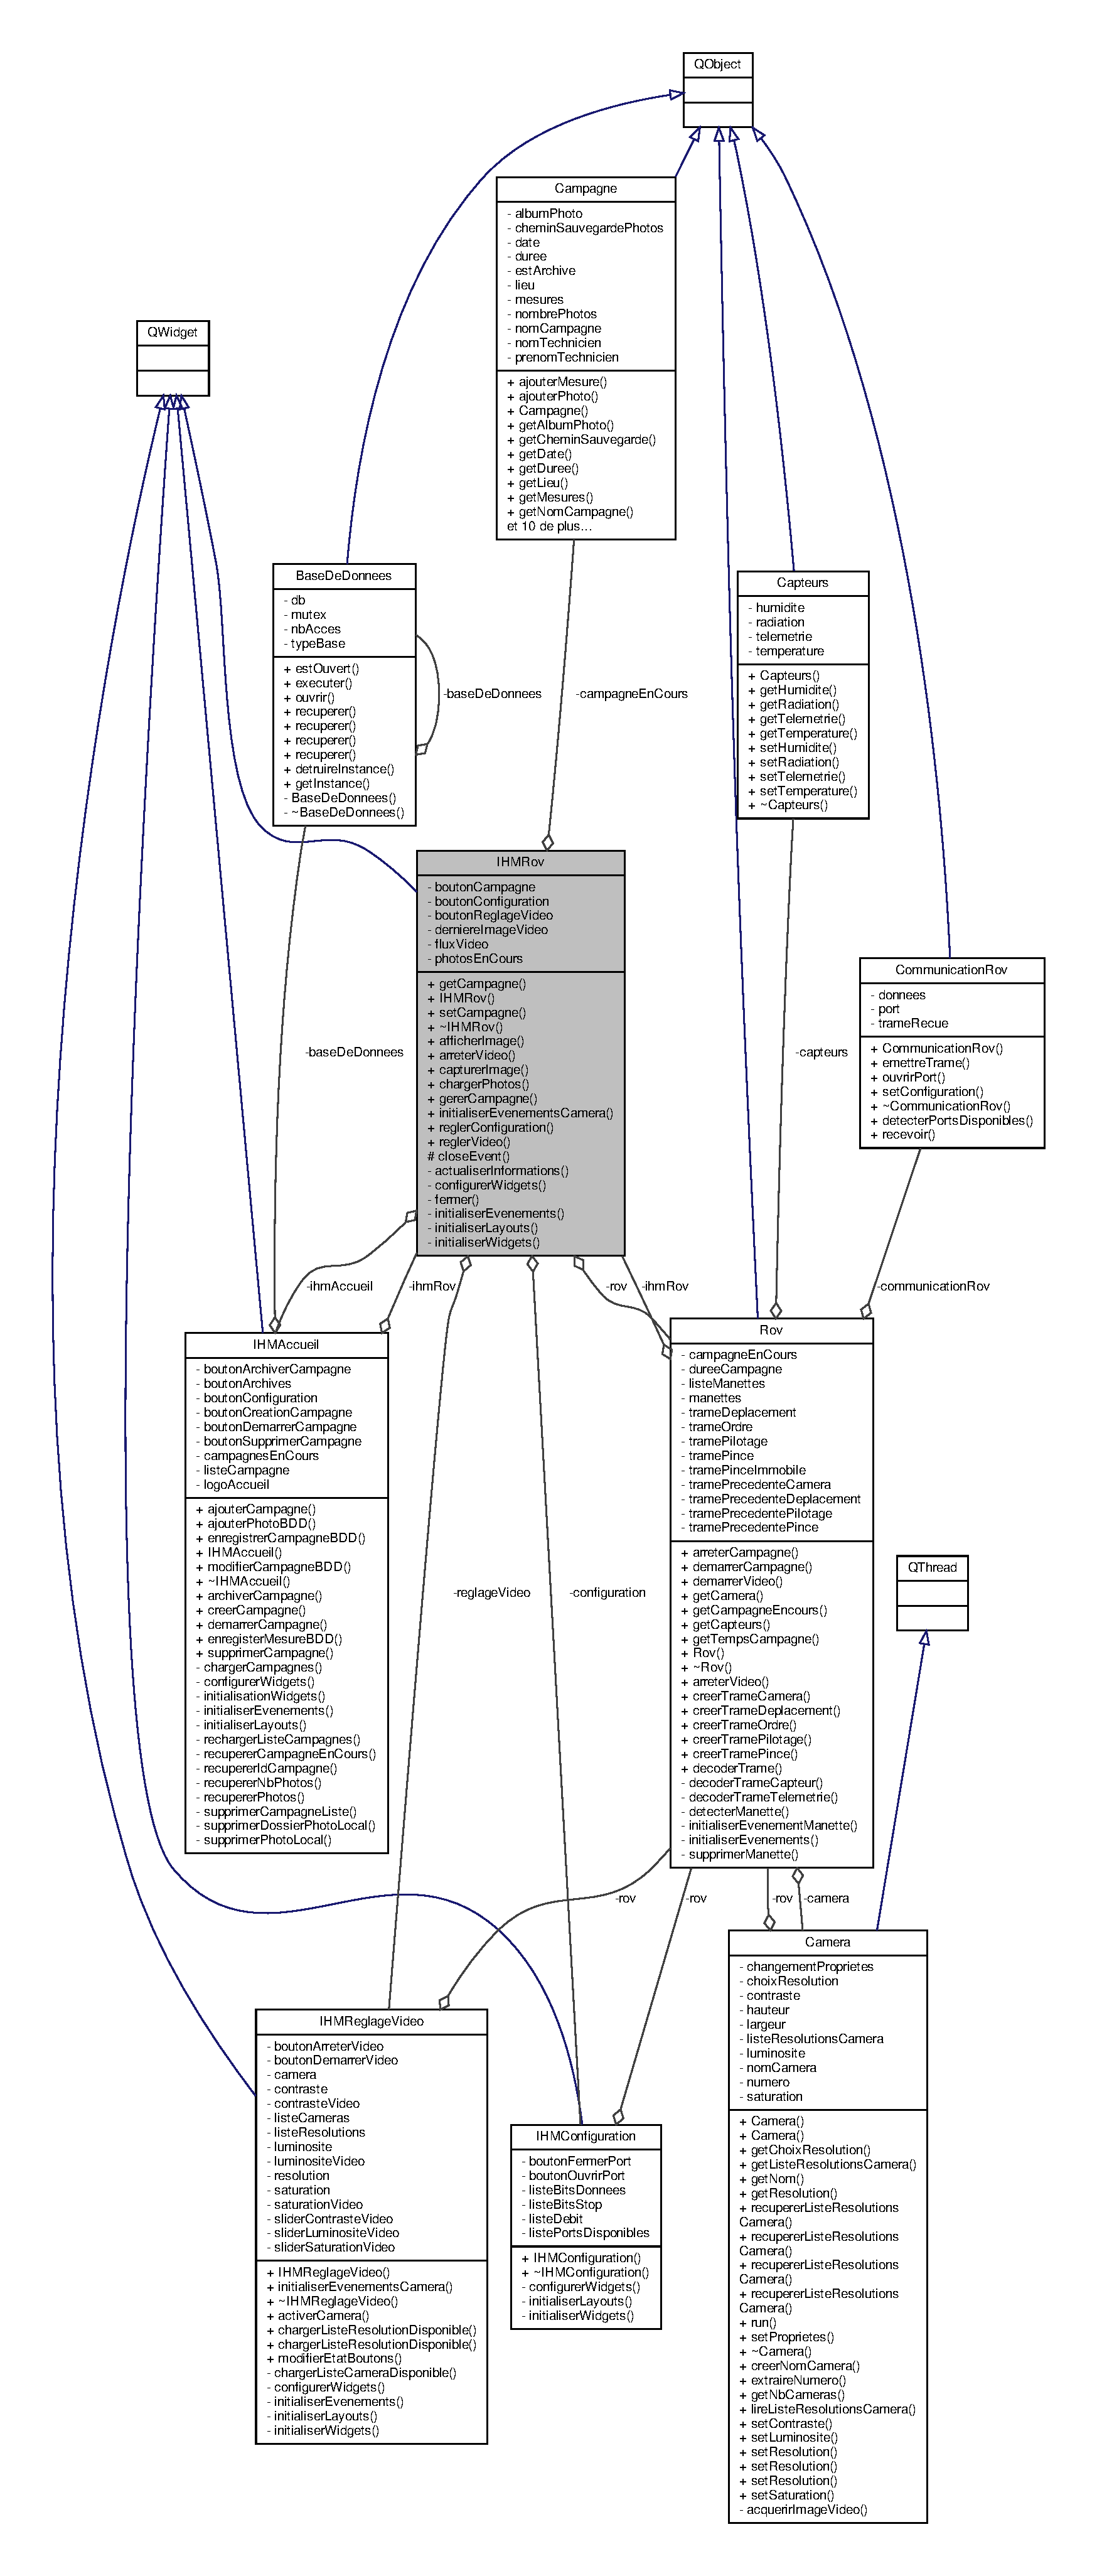
\includegraphics[height=550pt]{class_i_h_m_rov__coll__graph}
\end{center}
\end{figure}
\subsubsection*{Connecteurs publics}
\begin{DoxyCompactItemize}
\item 
void \hyperlink{class_i_h_m_rov_ae6e1c32c5dea20eb835f5c9036de8a5b}{afficher\+Image} (Q\+Pixmap image)
\begin{DoxyCompactList}\small\item\em Affiche la nouvelle image du flux vidéo dans l\textquotesingle{}ihm. \end{DoxyCompactList}\item 
void \hyperlink{class_i_h_m_rov_a81335964f1443d11e0929017b2f21267}{arreter\+Video} ()
\begin{DoxyCompactList}\small\item\em Déconnecte les événements liés à la caméra et modifie l\textquotesingle{}état des boutons de l\textquotesingle{}I\+HM. \end{DoxyCompactList}\item 
void \hyperlink{class_i_h_m_rov_a15fe4fd090a0171bb9ad24e28d3b978a}{capturer\+Image} (bool etat=false)
\begin{DoxyCompactList}\small\item\em Enregistre la dernière image du flux vidéo. \end{DoxyCompactList}\item 
void \hyperlink{class_i_h_m_rov_aae5c264f7a1b6d27c1d2e25574c88c5b}{charger\+Photos} ()
\begin{DoxyCompactList}\small\item\em Charge les photos disponible dans le conteneur album\+Photo de la classe campagne pour les afficher dans l\textquotesingle{}\hyperlink{class_i_h_m_album_photo}{I\+H\+M\+Album\+Photo}. \end{DoxyCompactList}\item 
void \hyperlink{class_i_h_m_rov_a3660d3b4bf61367534eae9d0c3618a5e}{gerer\+Campagne} ()
\begin{DoxyCompactList}\small\item\em Arrête la campagne en cours. \end{DoxyCompactList}\item 
void \hyperlink{class_i_h_m_rov_a955daa231d959666fa7ed01346b2b6ef}{initialiser\+Evenements\+Camera} ()
\begin{DoxyCompactList}\small\item\em Initialise les événements liés à la caméra. \end{DoxyCompactList}\item 
void \hyperlink{class_i_h_m_rov_a9b517b4891917634d64c903894bcc48b}{regler\+Configuration} ()
\begin{DoxyCompactList}\small\item\em Ouvre une nouvelle fenetre permettant de régler la communication. \end{DoxyCompactList}\item 
void \hyperlink{class_i_h_m_rov_a68653dfe09dbb9695797d60e9190366b}{regler\+Video} ()
\begin{DoxyCompactList}\small\item\em Ouvre une nouvelle fenetre permettant de régler l\textquotesingle{}affichage vidéo. \end{DoxyCompactList}\end{DoxyCompactItemize}
\subsubsection*{Fonctions membres publiques}
\begin{DoxyCompactItemize}
\item 
\hyperlink{class_campagne}{Campagne} $\ast$ \hyperlink{class_i_h_m_rov_ab3e8686eef9233b4c1e6711cf1c4576a}{get\+Campagne} ()
\begin{DoxyCompactList}\small\item\em Retourne l\textquotesingle{}objet campagne en cours. \end{DoxyCompactList}\item 
\hyperlink{class_i_h_m_rov_a403274da2bd4ca316f2f1b64a48a315b}{I\+H\+M\+Rov} (\hyperlink{class_i_h_m_accueil}{I\+H\+M\+Accueil} $\ast$\hyperlink{class_i_h_m_rov_aa22f6fe8daf5c67071ec02a348e5cc3e}{ihm\+Accueil}, \hyperlink{class_q_widget}{Q\+Widget} $\ast$parent=nullptr)
\begin{DoxyCompactList}\small\item\em Constructeur de la classe \hyperlink{class_i_h_m_rov}{I\+H\+M\+Rov}. \end{DoxyCompactList}\item 
void \hyperlink{class_i_h_m_rov_a301a0b8cb323c2c9de71df9070bb7555}{set\+Campagne} (\hyperlink{class_campagne}{Campagne} $\ast$campagne)
\begin{DoxyCompactList}\small\item\em Associe une campagne a la campagne en cours du rov. \end{DoxyCompactList}\item 
\hyperlink{class_i_h_m_rov_ab861463889934a3b6083b7a29c6adf45}{$\sim$\+I\+H\+M\+Rov} ()
\begin{DoxyCompactList}\small\item\em Destructeur de la classe \hyperlink{class_i_h_m_rov}{I\+H\+M\+Rov}. \end{DoxyCompactList}\end{DoxyCompactItemize}
\subsubsection*{Fonctions membres protégées}
\begin{DoxyCompactItemize}
\item 
void \hyperlink{class_i_h_m_rov_a68b11818797a6444a8fab81b7b45f670}{close\+Event} (Q\+Close\+Event $\ast$event)
\begin{DoxyCompactList}\small\item\em Gêre l\textquotesingle{}état de la campagne lors de la fermeture forcé de la fenêtre ihm\+Rov. \end{DoxyCompactList}\end{DoxyCompactItemize}
\subsubsection*{Fonctions membres privées}
\begin{DoxyCompactItemize}
\item 
void \hyperlink{class_i_h_m_rov_a58ba3661c111c9ab2d6f1e3c52f4ec21}{actualiser\+Informations} (Q\+Pixmap \&image)
\begin{DoxyCompactList}\small\item\em Actualise les informations incrusté dans l\textquotesingle{}image (heure, données capteur, durée missions) \end{DoxyCompactList}\item 
void \hyperlink{class_i_h_m_rov_aba47130fb875a01eefa09bc875affe6c}{configurer\+Widgets} ()
\begin{DoxyCompactList}\small\item\em Configure l\textquotesingle{}état des widgets à la création de l\textquotesingle{}I\+HM. \end{DoxyCompactList}\item 
void \hyperlink{class_i_h_m_rov_ac0c8c09dc2ef1c06e1008647dcd2d6b8}{fermer} ()
\begin{DoxyCompactList}\small\item\em Arrête la campagne et ferme l\textquotesingle{}ihm\+Rov. \end{DoxyCompactList}\item 
void \hyperlink{class_i_h_m_rov_a61e34efc084bba9934bce0d91448ea04}{initialiser\+Evenements} ()
\begin{DoxyCompactList}\small\item\em Initialise les événements de l\textquotesingle{}I\+HM. \end{DoxyCompactList}\item 
void \hyperlink{class_i_h_m_rov_aa900473297415bf43a13c4152034135a}{initialiser\+Layouts} ()
\begin{DoxyCompactList}\small\item\em Initialise les layouts de l\textquotesingle{}I\+HM. \end{DoxyCompactList}\item 
void \hyperlink{class_i_h_m_rov_a77d08efdfc3292d215af4df0e1af33a8}{initialiser\+Widgets} ()
\begin{DoxyCompactList}\small\item\em Initialise les widgets de l\textquotesingle{}I\+HM. \end{DoxyCompactList}\end{DoxyCompactItemize}
\subsubsection*{Attributs privés}
\begin{DoxyCompactItemize}
\item 
Q\+Push\+Button $\ast$ \hyperlink{class_i_h_m_rov_a324be23537f48127c49b943aa439a978}{bouton\+Campagne}
\begin{DoxyCompactList}\small\item\em Bouton permettant de mettre en pause la campagne en cours. \end{DoxyCompactList}\item 
Q\+Push\+Button $\ast$ \hyperlink{class_i_h_m_rov_aea67721180bf155892a297b3c39309c5}{bouton\+Configuration}
\begin{DoxyCompactList}\small\item\em Bouton permettant d\textquotesingle{}accéder à la configuration de la communication. \end{DoxyCompactList}\item 
Q\+Push\+Button $\ast$ \hyperlink{class_i_h_m_rov_a57cb3bea4f1f9149d730ccc5688581fc}{bouton\+Reglage\+Video}
\begin{DoxyCompactList}\small\item\em Bouton permettant d\textquotesingle{}accéder aux reglage de la vidéo. \end{DoxyCompactList}\item 
\hyperlink{class_campagne}{Campagne} $\ast$ \hyperlink{class_i_h_m_rov_af0475e935531b7331f097ae13d07989b}{campagne\+En\+Cours}
\begin{DoxyCompactList}\small\item\em Instance d\textquotesingle{}un objet \hyperlink{class_campagne}{Campagne} possédant les informations de la campagne en cours. \end{DoxyCompactList}\item 
\hyperlink{class_i_h_m_configuration}{I\+H\+M\+Configuration} $\ast$ \hyperlink{class_i_h_m_rov_a29f4de081899d8830376f1ad27e74647}{configuration}
\begin{DoxyCompactList}\small\item\em Instance d\textquotesingle{}un objet \hyperlink{class_i_h_m_configuration}{I\+H\+M\+Configuration} permettant de modifier les reglages de la communication. \end{DoxyCompactList}\item 
Q\+Pixmap \hyperlink{class_i_h_m_rov_a2081e30323773ee895199ec026d82fc8}{derniere\+Image\+Video}
\begin{DoxyCompactList}\small\item\em Dernière image reçue du flux vidéo. \end{DoxyCompactList}\item 
Q\+Label $\ast$ \hyperlink{class_i_h_m_rov_acdeabe02e1431b5c1817cb2a89debd0a}{flux\+Video}
\begin{DoxyCompactList}\small\item\em Emplacement permettant d\textquotesingle{}accueiller le flux vidéo. \end{DoxyCompactList}\item 
\hyperlink{class_i_h_m_accueil}{I\+H\+M\+Accueil} $\ast$ \hyperlink{class_i_h_m_rov_aa22f6fe8daf5c67071ec02a348e5cc3e}{ihm\+Accueil}
\begin{DoxyCompactList}\small\item\em Relation entre l\textquotesingle{}ihm\+Accueil et l\textquotesingle{}ihm\+Rov. \end{DoxyCompactList}\item 
Q\+Push\+Button $\ast$ \hyperlink{class_i_h_m_rov_a0896dea1a2d901a7cf43a344e22fc66d}{photos\+En\+Cours}
\begin{DoxyCompactList}\small\item\em Bouton permettant d\textquotesingle{}accéder aux photo prise en cours de campagne. \end{DoxyCompactList}\item 
\hyperlink{class_i_h_m_reglage_video}{I\+H\+M\+Reglage\+Video} $\ast$ \hyperlink{class_i_h_m_rov_a6baa53853d29151404e6ae3dec5d2003}{reglage\+Video}
\begin{DoxyCompactList}\small\item\em Instance d\textquotesingle{}un objet reglage\+Vidéo permettant de modifier les reglages du flux vidéo. \end{DoxyCompactList}\item 
\hyperlink{class_rov}{Rov} $\ast$ \hyperlink{class_i_h_m_rov_a777ca33fdb295ba6b6773e880356fa1e}{rov}
\begin{DoxyCompactList}\small\item\em Instance d\textquotesingle{}un objet rov possédant le controle sur les autres classes. \end{DoxyCompactList}\end{DoxyCompactItemize}


\subsubsection{Description détaillée}
I\+HM permettant d\textquotesingle{}obtenir le flux vidéo en direct placé sur le robot et d\textquotesingle{}obtenir les informations relatifs à ses capteurs. 

Définition à la ligne \hyperlink{ihmrov_8h_source_l00041}{41} du fichier \hyperlink{ihmrov_8h_source}{ihmrov.\+h}.



\subsubsection{Documentation des constructeurs et destructeur}
\mbox{\Hypertarget{class_i_h_m_rov_a403274da2bd4ca316f2f1b64a48a315b}\label{class_i_h_m_rov_a403274da2bd4ca316f2f1b64a48a315b}} 
\index{I\+H\+M\+Rov@{I\+H\+M\+Rov}!I\+H\+M\+Rov@{I\+H\+M\+Rov}}
\index{I\+H\+M\+Rov@{I\+H\+M\+Rov}!I\+H\+M\+Rov@{I\+H\+M\+Rov}}
\paragraph{\texorpdfstring{I\+H\+M\+Rov()}{IHMRov()}}
{\footnotesize\ttfamily I\+H\+M\+Rov\+::\+I\+H\+M\+Rov (\begin{DoxyParamCaption}\item[{\hyperlink{class_i_h_m_accueil}{I\+H\+M\+Accueil} $\ast$}]{ihm\+Accueil,  }\item[{\hyperlink{class_q_widget}{Q\+Widget} $\ast$}]{parent = {\ttfamily nullptr} }\end{DoxyParamCaption})}



Constructeur de la classe \hyperlink{class_i_h_m_rov}{I\+H\+M\+Rov}. 


\begin{DoxyParams}{Paramètres}
{\em ihm\+Accueil} & \\
\hline
{\em parent} & \\
\hline
\end{DoxyParams}


Définition à la ligne \hyperlink{ihmrov_8cpp_source_l00015}{15} du fichier \hyperlink{ihmrov_8cpp_source}{ihmrov.\+cpp}.



Références \hyperlink{ihmrov_8h_source_l00049}{configuration}, \hyperlink{ihmrov_8cpp_source_l00050}{configurer\+Widgets()}, \hyperlink{ihmrov_8cpp_source_l00098}{initialiser\+Evenements()}, \hyperlink{ihmrov_8cpp_source_l00061}{initialiser\+Layouts()}, \hyperlink{ihmrov_8cpp_source_l00033}{initialiser\+Widgets()}, \hyperlink{ihmrov_8h_source_l00048}{reglage\+Video}, et \hyperlink{ihmrov_8h_source_l00047}{rov}.


\begin{DoxyCode}
00015                                                       : \hyperlink{class_q_widget}{QWidget}(parent), 
      \hyperlink{class_i_h_m_rov_af0475e935531b7331f097ae13d07989b}{campagneEnCours}(\textcolor{keyword}{nullptr}), \hyperlink{class_i_h_m_rov_aa22f6fe8daf5c67071ec02a348e5cc3e}{ihmAccueil}(ihmAccueil)
00016 \{    
00017     qDebug() << Q\_FUNC\_INFO << \textcolor{keyword}{this} << \textcolor{stringliteral}{"width"} << qApp->desktop()->screen()->width() << \textcolor{stringliteral}{"height"} << qApp->
      desktop()->screen()->height();
00018     \hyperlink{class_i_h_m_rov_a777ca33fdb295ba6b6773e880356fa1e}{rov} = \textcolor{keyword}{new} \hyperlink{class_rov}{Rov}(\textcolor{keyword}{this});
00019     \hyperlink{class_i_h_m_rov_a6baa53853d29151404e6ae3dec5d2003}{reglageVideo} = \textcolor{keyword}{nullptr};
00020     \hyperlink{class_i_h_m_rov_a29f4de081899d8830376f1ad27e74647}{configuration} = \textcolor{keyword}{nullptr};
00021 
00022     \hyperlink{class_i_h_m_rov_a77d08efdfc3292d215af4df0e1af33a8}{initialiserWidgets}();
00023     \hyperlink{class_i_h_m_rov_aba47130fb875a01eefa09bc875affe6c}{configurerWidgets}();
00024     \hyperlink{class_i_h_m_rov_aa900473297415bf43a13c4152034135a}{initialiserLayouts}();
00025     \hyperlink{class_i_h_m_rov_a61e34efc084bba9934bce0d91448ea04}{initialiserEvenements}();
00026 \}
\end{DoxyCode}
\mbox{\Hypertarget{class_i_h_m_rov_ab861463889934a3b6083b7a29c6adf45}\label{class_i_h_m_rov_ab861463889934a3b6083b7a29c6adf45}} 
\index{I\+H\+M\+Rov@{I\+H\+M\+Rov}!````~I\+H\+M\+Rov@{$\sim$\+I\+H\+M\+Rov}}
\index{````~I\+H\+M\+Rov@{$\sim$\+I\+H\+M\+Rov}!I\+H\+M\+Rov@{I\+H\+M\+Rov}}
\paragraph{\texorpdfstring{$\sim$\+I\+H\+M\+Rov()}{~IHMRov()}}
{\footnotesize\ttfamily I\+H\+M\+Rov\+::$\sim$\+I\+H\+M\+Rov (\begin{DoxyParamCaption}{ }\end{DoxyParamCaption})}



Destructeur de la classe \hyperlink{class_i_h_m_rov}{I\+H\+M\+Rov}. 



Définition à la ligne \hyperlink{ihmrov_8cpp_source_l00028}{28} du fichier \hyperlink{ihmrov_8cpp_source}{ihmrov.\+cpp}.


\begin{DoxyCode}
00029 \{
00030     qDebug() << Q\_FUNC\_INFO;
00031 \}
\end{DoxyCode}


\subsubsection{Documentation des fonctions membres}
\mbox{\Hypertarget{class_i_h_m_rov_a58ba3661c111c9ab2d6f1e3c52f4ec21}\label{class_i_h_m_rov_a58ba3661c111c9ab2d6f1e3c52f4ec21}} 
\index{I\+H\+M\+Rov@{I\+H\+M\+Rov}!actualiser\+Informations@{actualiser\+Informations}}
\index{actualiser\+Informations@{actualiser\+Informations}!I\+H\+M\+Rov@{I\+H\+M\+Rov}}
\paragraph{\texorpdfstring{actualiser\+Informations()}{actualiserInformations()}}
{\footnotesize\ttfamily void I\+H\+M\+Rov\+::actualiser\+Informations (\begin{DoxyParamCaption}\item[{Q\+Pixmap \&}]{image }\end{DoxyParamCaption})\hspace{0.3cm}{\ttfamily [private]}}



Actualise les informations incrusté dans l\textquotesingle{}image (heure, données capteur, durée missions) 


\begin{DoxyParams}{Paramètres}
{\em image} & \\
\hline
\end{DoxyParams}
\begin{DoxyRefDesc}{A faire}
\item[\hyperlink{todo__todo000001}{A faire}]Tenir compte de la résolution de l\textquotesingle{}image \end{DoxyRefDesc}


Définition à la ligne \hyperlink{ihmrov_8cpp_source_l00110}{110} du fichier \hyperlink{ihmrov_8cpp_source}{ihmrov.\+cpp}.



Références \hyperlink{rov_8cpp_source_l00149}{Rov\+::get\+Capteurs()}, \hyperlink{capteurs_8cpp_source_l00054}{Capteurs\+::get\+Radiation()}, \hyperlink{capteurs_8cpp_source_l00039}{Capteurs\+::get\+Telemetrie()}, \hyperlink{capteurs_8cpp_source_l00044}{Capteurs\+::get\+Temperature()}, \hyperlink{rov_8cpp_source_l00154}{Rov\+::get\+Temps\+Campagne()}, et \hyperlink{ihmrov_8h_source_l00047}{rov}.



Référencé par \hyperlink{ihmrov_8cpp_source_l00154}{afficher\+Image()}.


\begin{DoxyCode}
00111 \{
00112     QPainter p(&image);
00113     p.setPen(Qt::darkRed);
00114     p.setFont(QFont(\textcolor{stringliteral}{"Arial"}, 20));
00115 
00120     QImage logoHeure(qApp->applicationDirPath() + \textcolor{stringliteral}{"/images/logo\_heure.png"});
00121     p.drawImage(5, 6, logoHeure.scaled(20,20));
00122     p.drawText(30, 25, QTime::currentTime().toString());
00123 
00124     QImage logoDuree(qApp->applicationDirPath() + \textcolor{stringliteral}{"/images/logo\_duree.png"});
00125     p.drawImage(600, 6, logoDuree.scaled(20,20));
00126     p.drawText(490, 25, \hyperlink{class_i_h_m_rov_a777ca33fdb295ba6b6773e880356fa1e}{rov}->\hyperlink{class_rov_aa977585d4377a57281004fd57208635a}{getTempsCampagne}());
00127 
00128     QImage logoTemperature(qApp->applicationDirPath() + \textcolor{stringliteral}{"/images/logo\_temperature.png"});
00129     p.drawImage(5, 430, logoTemperature.scaled(20,40));
00130     p.drawText(35, 460, \hyperlink{class_i_h_m_rov_a777ca33fdb295ba6b6773e880356fa1e}{rov}->\hyperlink{class_rov_a7e231245b39e7cc8026324e337b34c64}{getCapteurs}()->\hyperlink{class_capteurs_aa1346e5cbea9e37afc3694a0ea86bd99}{getTemperature}() + \textcolor{stringliteral}{" °C"});
00131 
00132     QImage logoRadiation(qApp->applicationDirPath() + \textcolor{stringliteral}{"/images/logo\_radiation.png"});
00133     p.drawImage(160, 430, logoRadiation.scaled(40,40));
00134     p.drawText(210, 460, \hyperlink{class_i_h_m_rov_a777ca33fdb295ba6b6773e880356fa1e}{rov}->\hyperlink{class_rov_a7e231245b39e7cc8026324e337b34c64}{getCapteurs}()->\hyperlink{class_capteurs_aaee3d64c752b09f8674fa62907f38cbc}{getRadiation}() + \textcolor{stringliteral}{" uS/h"});
00135 
00136     QImage logoObstacle(qApp->applicationDirPath() + \textcolor{stringliteral}{"/images/logo\_telemetrie.png"});
00137     p.drawImage(400, 430, logoObstacle.scaled(40,40));
00138     p.drawText(450, 460, \textcolor{stringliteral}{"Obstacle : "} + \hyperlink{class_i_h_m_rov_a777ca33fdb295ba6b6773e880356fa1e}{rov}->\hyperlink{class_rov_a7e231245b39e7cc8026324e337b34c64}{getCapteurs}()->
      \hyperlink{class_capteurs_ad8c2c486e92cc537dc014035b5634b60}{getTelemetrie}() + \textcolor{stringliteral}{" cm"});
00139 
00140     p.end();
00141 \}
\end{DoxyCode}
\mbox{\Hypertarget{class_i_h_m_rov_ae6e1c32c5dea20eb835f5c9036de8a5b}\label{class_i_h_m_rov_ae6e1c32c5dea20eb835f5c9036de8a5b}} 
\index{I\+H\+M\+Rov@{I\+H\+M\+Rov}!afficher\+Image@{afficher\+Image}}
\index{afficher\+Image@{afficher\+Image}!I\+H\+M\+Rov@{I\+H\+M\+Rov}}
\paragraph{\texorpdfstring{afficher\+Image}{afficherImage}}
{\footnotesize\ttfamily void I\+H\+M\+Rov\+::afficher\+Image (\begin{DoxyParamCaption}\item[{Q\+Pixmap}]{image }\end{DoxyParamCaption})\hspace{0.3cm}{\ttfamily [slot]}}



Affiche la nouvelle image du flux vidéo dans l\textquotesingle{}ihm. 


\begin{DoxyParams}{Paramètres}
{\em image} & \\
\hline
\end{DoxyParams}


Définition à la ligne \hyperlink{ihmrov_8cpp_source_l00154}{154} du fichier \hyperlink{ihmrov_8cpp_source}{ihmrov.\+cpp}.



Références \hyperlink{ihmrov_8cpp_source_l00110}{actualiser\+Informations()}, \hyperlink{ihmrov_8h_source_l00053}{derniere\+Image\+Video}, et \hyperlink{ihmrov_8h_source_l00050}{flux\+Video}.


\begin{DoxyCode}
00155 \{
00156     \hyperlink{class_i_h_m_rov_a2081e30323773ee895199ec026d82fc8}{derniereImageVideo} = image;
00157     \hyperlink{class_i_h_m_rov_a58ba3661c111c9ab2d6f1e3c52f4ec21}{actualiserInformations}(image);
00158     \hyperlink{class_i_h_m_rov_acdeabe02e1431b5c1817cb2a89debd0a}{fluxVideo}->setPixmap(image);
00159 \}
\end{DoxyCode}
\mbox{\Hypertarget{class_i_h_m_rov_a81335964f1443d11e0929017b2f21267}\label{class_i_h_m_rov_a81335964f1443d11e0929017b2f21267}} 
\index{I\+H\+M\+Rov@{I\+H\+M\+Rov}!arreter\+Video@{arreter\+Video}}
\index{arreter\+Video@{arreter\+Video}!I\+H\+M\+Rov@{I\+H\+M\+Rov}}
\paragraph{\texorpdfstring{arreter\+Video}{arreterVideo}}
{\footnotesize\ttfamily void I\+H\+M\+Rov\+::arreter\+Video (\begin{DoxyParamCaption}{ }\end{DoxyParamCaption})\hspace{0.3cm}{\ttfamily [slot]}}



Déconnecte les événements liés à la caméra et modifie l\textquotesingle{}état des boutons de l\textquotesingle{}I\+HM. 



Définition à la ligne \hyperlink{ihmrov_8cpp_source_l00234}{234} du fichier \hyperlink{ihmrov_8cpp_source}{ihmrov.\+cpp}.



Références \hyperlink{ihmreglagevideo_8cpp_source_l00212}{I\+H\+M\+Reglage\+Video\+::modifier\+Etat\+Boutons()}, et \hyperlink{ihmrov_8h_source_l00048}{reglage\+Video}.



Référencé par \hyperlink{rov_8cpp_source_l00263}{Rov\+::arreter\+Video()}.


\begin{DoxyCode}
00235 \{
00236     \hyperlink{class_i_h_m_rov_a6baa53853d29151404e6ae3dec5d2003}{reglageVideo}->\hyperlink{class_i_h_m_reglage_video_ac838581ba03f52e79064cb91ebabb35d}{modifierEtatBoutons}();
00237 \}
\end{DoxyCode}
\mbox{\Hypertarget{class_i_h_m_rov_a15fe4fd090a0171bb9ad24e28d3b978a}\label{class_i_h_m_rov_a15fe4fd090a0171bb9ad24e28d3b978a}} 
\index{I\+H\+M\+Rov@{I\+H\+M\+Rov}!capturer\+Image@{capturer\+Image}}
\index{capturer\+Image@{capturer\+Image}!I\+H\+M\+Rov@{I\+H\+M\+Rov}}
\paragraph{\texorpdfstring{capturer\+Image}{capturerImage}}
{\footnotesize\ttfamily void I\+H\+M\+Rov\+::capturer\+Image (\begin{DoxyParamCaption}\item[{bool}]{etat = {\ttfamily false} }\end{DoxyParamCaption})\hspace{0.3cm}{\ttfamily [slot]}}



Enregistre la dernière image du flux vidéo. 


\begin{DoxyParams}{Paramètres}
{\em etat} & \\
\hline
\end{DoxyParams}


Définition à la ligne \hyperlink{ihmrov_8cpp_source_l00179}{179} du fichier \hyperlink{ihmrov_8cpp_source}{ihmrov.\+cpp}.



Références \hyperlink{ihmalbumphoto_8h_source_l00024}{Photo\+::a\+Garder}, \hyperlink{campagne_8cpp_source_l00080}{Campagne\+::ajouter\+Photo()}, \hyperlink{ihmaccueil_8cpp_source_l00313}{I\+H\+M\+Accueil\+::ajouter\+Photo\+B\+D\+D()}, \hyperlink{ihmrov_8h_source_l00045}{campagne\+En\+Cours}, \hyperlink{ihmalbumphoto_8h_source_l00025}{Photo\+::chemin\+Sauvegarde}, \hyperlink{ihmalbumphoto_8h_source_l00023}{Photo\+::dateheure}, \hyperlink{ihmrov_8h_source_l00053}{derniere\+Image\+Video}, \hyperlink{campagne_8cpp_source_l00055}{Campagne\+::get\+Chemin\+Sauvegarde()}, \hyperlink{campagne_8cpp_source_l00019}{Campagne\+::get\+Nom\+Campagne()}, \hyperlink{ihmrov_8h_source_l00046}{ihm\+Accueil}, \hyperlink{ihmalbumphoto_8h_source_l00022}{Photo\+::image}, et \hyperlink{campagne_8cpp_source_l00105}{Campagne\+::incremente\+Nombre\+Photo()}.



Référencé par \hyperlink{ihmrov_8cpp_source_l00098}{initialiser\+Evenements()}, et \hyperlink{ihmrov_8cpp_source_l00033}{initialiser\+Widgets()}.


\begin{DoxyCode}
00180 \{
00181 \textcolor{preprocessor}{    #ifndef PAS\_DE\_MANETTE}
00182     \textcolor{keywordflow}{if}(etat)
00183 \textcolor{preprocessor}{    #endif}
00184     \textcolor{comment}{//Q\_UNUSED(etat)}
00185     \{        
00186         \hyperlink{struct_photo}{Photo} photo;
00187 
00188         photo.\hyperlink{struct_photo_aa6ecfed8082bea5af2905208308a6adb}{image} = \hyperlink{class_i_h_m_rov_a2081e30323773ee895199ec026d82fc8}{derniereImageVideo};
00189         photo.\hyperlink{struct_photo_a0ac4d5bba2d119ca73ba949d18a557bd}{dateheure} = QTime::currentTime();
00190         photo.\hyperlink{struct_photo_afec1baefdd7d036432494bbb33b21366}{aGarder} = \textcolor{keyword}{true};
00191         photo.\hyperlink{struct_photo_a3c28eb9ad160b65deb46a72146a1d14f}{cheminSauvegarde} = \hyperlink{class_i_h_m_rov_af0475e935531b7331f097ae13d07989b}{campagneEnCours}->
      \hyperlink{class_campagne_ad752790357417d83a93056d9c9689a16}{getCheminSauvegarde}() + \textcolor{stringliteral}{"/"} + \hyperlink{class_i_h_m_rov_af0475e935531b7331f097ae13d07989b}{campagneEnCours}->
      \hyperlink{class_campagne_a99a682fcb8e5a3f8c2aff7a44eb2c930}{getNomCampagne}() + \textcolor{stringliteral}{"/"} + \textcolor{stringliteral}{"Capture\_"} + QString::number(
      \hyperlink{class_i_h_m_rov_af0475e935531b7331f097ae13d07989b}{campagneEnCours}->\hyperlink{class_campagne_ab6a893a28bc18e054d2d19d2671ce6da}{incrementeNombrePhoto}());
00192 
00193         \hyperlink{class_i_h_m_rov_af0475e935531b7331f097ae13d07989b}{campagneEnCours}->\hyperlink{class_campagne_a472029bf46646d136a750dbaa7a3155f}{ajouterPhoto}(photo);
00194         qDebug() << Q\_FUNC\_INFO << \textcolor{stringliteral}{"Photo capturée"};
00195 
00196         photo.\hyperlink{struct_photo_aa6ecfed8082bea5af2905208308a6adb}{image}.save(photo.\hyperlink{struct_photo_a3c28eb9ad160b65deb46a72146a1d14f}{cheminSauvegarde}, \textcolor{stringliteral}{"PNG"});
00197 
00198         \hyperlink{class_i_h_m_rov_aa22f6fe8daf5c67071ec02a348e5cc3e}{ihmAccueil}->\hyperlink{class_i_h_m_accueil_aa27c7334efe44c8c4cd582df6581fdff}{ajouterPhotoBDD}(photo, 
      \hyperlink{class_i_h_m_rov_af0475e935531b7331f097ae13d07989b}{campagneEnCours});
00199     \}
00200 \}
\end{DoxyCode}
\mbox{\Hypertarget{class_i_h_m_rov_aae5c264f7a1b6d27c1d2e25574c88c5b}\label{class_i_h_m_rov_aae5c264f7a1b6d27c1d2e25574c88c5b}} 
\index{I\+H\+M\+Rov@{I\+H\+M\+Rov}!charger\+Photos@{charger\+Photos}}
\index{charger\+Photos@{charger\+Photos}!I\+H\+M\+Rov@{I\+H\+M\+Rov}}
\paragraph{\texorpdfstring{charger\+Photos}{chargerPhotos}}
{\footnotesize\ttfamily void I\+H\+M\+Rov\+::charger\+Photos (\begin{DoxyParamCaption}{ }\end{DoxyParamCaption})\hspace{0.3cm}{\ttfamily [slot]}}



Charge les photos disponible dans le conteneur album\+Photo de la classe campagne pour les afficher dans l\textquotesingle{}\hyperlink{class_i_h_m_album_photo}{I\+H\+M\+Album\+Photo}. 



Définition à la ligne \hyperlink{ihmrov_8cpp_source_l00223}{223} du fichier \hyperlink{ihmrov_8cpp_source}{ihmrov.\+cpp}.



Références \hyperlink{ihmrov_8h_source_l00045}{campagne\+En\+Cours}, \hyperlink{campagne_8cpp_source_l00070}{Campagne\+::get\+Album\+Photo()}, et \hyperlink{ihmalbumphoto_8cpp_source_l00038}{I\+H\+M\+Album\+Photo\+::ouvrir\+Album\+Photos()}.



Référencé par \hyperlink{ihmrov_8cpp_source_l00098}{initialiser\+Evenements()}.


\begin{DoxyCode}
00224 \{
00225     \hyperlink{class_i_h_m_album_photo}{IHMAlbumPhoto} *ihmAlbumPhoto = \textcolor{keyword}{new} \hyperlink{class_i_h_m_album_photo}{IHMAlbumPhoto}(\textcolor{keyword}{this});
00226     ihmAlbumPhoto->\hyperlink{class_i_h_m_album_photo_a5aa9a9c1b04e00eaec1581e92649535f}{ouvrirAlbumPhotos}(\hyperlink{class_i_h_m_rov_af0475e935531b7331f097ae13d07989b}{campagneEnCours}->
      \hyperlink{class_campagne_abec90fcbc0c4ded45caaac9adb454add}{getAlbumPhoto}());
00227 \}
\end{DoxyCode}
\mbox{\Hypertarget{class_i_h_m_rov_a68b11818797a6444a8fab81b7b45f670}\label{class_i_h_m_rov_a68b11818797a6444a8fab81b7b45f670}} 
\index{I\+H\+M\+Rov@{I\+H\+M\+Rov}!close\+Event@{close\+Event}}
\index{close\+Event@{close\+Event}!I\+H\+M\+Rov@{I\+H\+M\+Rov}}
\paragraph{\texorpdfstring{close\+Event()}{closeEvent()}}
{\footnotesize\ttfamily void I\+H\+M\+Rov\+::close\+Event (\begin{DoxyParamCaption}\item[{Q\+Close\+Event $\ast$}]{event }\end{DoxyParamCaption})\hspace{0.3cm}{\ttfamily [protected]}}



Gêre l\textquotesingle{}état de la campagne lors de la fermeture forcé de la fenêtre ihm\+Rov. 


\begin{DoxyParams}{Paramètres}
{\em event} & \\
\hline
\end{DoxyParams}


Définition à la ligne \hyperlink{ihmrov_8cpp_source_l00239}{239} du fichier \hyperlink{ihmrov_8cpp_source}{ihmrov.\+cpp}.



Références \hyperlink{ihmrov_8cpp_source_l00253}{fermer()}, \hyperlink{rov_8cpp_source_l00175}{Rov\+::get\+Campagne\+Encours()}, et \hyperlink{ihmrov_8h_source_l00047}{rov}.


\begin{DoxyCode}
00240 \{
00241     qDebug() << Q\_FUNC\_INFO << \hyperlink{class_i_h_m_rov_a777ca33fdb295ba6b6773e880356fa1e}{rov}->\hyperlink{class_rov_a59d1a6d2ca83324e6efc0b74f2cff686}{getCampagneEncours}();
00242     \textcolor{keywordflow}{if}(\hyperlink{class_i_h_m_rov_a777ca33fdb295ba6b6773e880356fa1e}{rov}->\hyperlink{class_rov_a59d1a6d2ca83324e6efc0b74f2cff686}{getCampagneEncours}())
00243     \{
00244         \hyperlink{class_i_h_m_rov_ac0c8c09dc2ef1c06e1008647dcd2d6b8}{fermer}();
00245         \textcolor{keyword}{event}->accept(); \textcolor{comment}{// -> close}
00246     \}
00247     \textcolor{keywordflow}{else}
00248     \{
00249         \textcolor{keyword}{event}->ignore();
00250     \}
00251 \}
\end{DoxyCode}
\mbox{\Hypertarget{class_i_h_m_rov_aba47130fb875a01eefa09bc875affe6c}\label{class_i_h_m_rov_aba47130fb875a01eefa09bc875affe6c}} 
\index{I\+H\+M\+Rov@{I\+H\+M\+Rov}!configurer\+Widgets@{configurer\+Widgets}}
\index{configurer\+Widgets@{configurer\+Widgets}!I\+H\+M\+Rov@{I\+H\+M\+Rov}}
\paragraph{\texorpdfstring{configurer\+Widgets()}{configurerWidgets()}}
{\footnotesize\ttfamily void I\+H\+M\+Rov\+::configurer\+Widgets (\begin{DoxyParamCaption}{ }\end{DoxyParamCaption})\hspace{0.3cm}{\ttfamily [private]}}



Configure l\textquotesingle{}état des widgets à la création de l\textquotesingle{}I\+HM. 



Définition à la ligne \hyperlink{ihmrov_8cpp_source_l00050}{50} du fichier \hyperlink{ihmrov_8cpp_source}{ihmrov.\+cpp}.



Références \hyperlink{ihmrov_8h_source_l00050}{flux\+Video}, et \hyperlink{ihmrov_8h_source_l00027}{R\+A\+T\+IO}.



Référencé par \hyperlink{ihmrov_8cpp_source_l00015}{I\+H\+M\+Rov()}.


\begin{DoxyCode}
00051 \{    
00052     \textcolor{keywordtype}{int} width = int(qApp->desktop()->screen()->width() * \hyperlink{ihmrov_8h_a7e8b3c8482e593df0ace933ad3de22ee}{RATIO});
00053     \textcolor{keywordtype}{int} height = int(qApp->desktop()->screen()->height() * \hyperlink{ihmrov_8h_a7e8b3c8482e593df0ace933ad3de22ee}{RATIO});
00054     \hyperlink{class_i_h_m_rov_acdeabe02e1431b5c1817cb2a89debd0a}{fluxVideo}->setMinimumWidth(width);
00055     \hyperlink{class_i_h_m_rov_acdeabe02e1431b5c1817cb2a89debd0a}{fluxVideo}->setMinimumHeight(height);
00056     \hyperlink{class_i_h_m_rov_acdeabe02e1431b5c1817cb2a89debd0a}{fluxVideo}->setMaximumWidth(width);
00057     \hyperlink{class_i_h_m_rov_acdeabe02e1431b5c1817cb2a89debd0a}{fluxVideo}->setMaximumHeight(height);
00058     \hyperlink{class_i_h_m_rov_acdeabe02e1431b5c1817cb2a89debd0a}{fluxVideo}->setScaledContents(\textcolor{keyword}{true});
00059 \}
\end{DoxyCode}
\mbox{\Hypertarget{class_i_h_m_rov_ac0c8c09dc2ef1c06e1008647dcd2d6b8}\label{class_i_h_m_rov_ac0c8c09dc2ef1c06e1008647dcd2d6b8}} 
\index{I\+H\+M\+Rov@{I\+H\+M\+Rov}!fermer@{fermer}}
\index{fermer@{fermer}!I\+H\+M\+Rov@{I\+H\+M\+Rov}}
\paragraph{\texorpdfstring{fermer()}{fermer()}}
{\footnotesize\ttfamily void I\+H\+M\+Rov\+::fermer (\begin{DoxyParamCaption}{ }\end{DoxyParamCaption})\hspace{0.3cm}{\ttfamily [private]}}



Arrête la campagne et ferme l\textquotesingle{}ihm\+Rov. 



Définition à la ligne \hyperlink{ihmrov_8cpp_source_l00253}{253} du fichier \hyperlink{ihmrov_8cpp_source}{ihmrov.\+cpp}.



Références \hyperlink{rov_8cpp_source_l00136}{Rov\+::arreter\+Campagne()}, \hyperlink{ihmrov_8h_source_l00057}{bouton\+Campagne}, \hyperlink{ihmrov_8h_source_l00045}{campagne\+En\+Cours}, \hyperlink{ihmrov_8h_source_l00049}{configuration}, \hyperlink{ihmrov_8h_source_l00046}{ihm\+Accueil}, \hyperlink{ihmaccueil_8cpp_source_l00295}{I\+H\+M\+Accueil\+::modifier\+Campagne\+B\+D\+D()}, \hyperlink{ihmrov_8h_source_l00048}{reglage\+Video}, et \hyperlink{ihmrov_8h_source_l00047}{rov}.



Référencé par \hyperlink{ihmrov_8cpp_source_l00239}{close\+Event()}, et \hyperlink{ihmrov_8cpp_source_l00202}{gerer\+Campagne()}.


\begin{DoxyCode}
00254 \{
00255     \hyperlink{class_i_h_m_rov_a777ca33fdb295ba6b6773e880356fa1e}{rov}->\hyperlink{class_rov_ad53e8d86817c81f92e3113b0394bedc5}{arreterCampagne}();
00256     \textcolor{keyword}{delete} \hyperlink{class_i_h_m_rov_a6baa53853d29151404e6ae3dec5d2003}{reglageVideo};
00257     \textcolor{keyword}{delete} \hyperlink{class_i_h_m_rov_a29f4de081899d8830376f1ad27e74647}{configuration};
00258     \hyperlink{class_i_h_m_rov_a6baa53853d29151404e6ae3dec5d2003}{reglageVideo} = \textcolor{keyword}{nullptr};
00259     \hyperlink{class_i_h_m_rov_a29f4de081899d8830376f1ad27e74647}{configuration} = \textcolor{keyword}{nullptr};
00260     \hyperlink{class_i_h_m_rov_a324be23537f48127c49b943aa439a978}{boutonCampagne}->setText(QString::fromUtf8(\textcolor{stringliteral}{"Démarrer"}));
00261     \hyperlink{class_i_h_m_rov_aa22f6fe8daf5c67071ec02a348e5cc3e}{ihmAccueil}->\hyperlink{class_i_h_m_accueil_a7f1e5f71843a99cb44e3efb7191a6d07}{modifierCampagneBDD}(\hyperlink{class_i_h_m_rov_af0475e935531b7331f097ae13d07989b}{campagneEnCours});
00262     this->setVisible(\textcolor{keyword}{false});
00263     \hyperlink{class_i_h_m_rov_aa22f6fe8daf5c67071ec02a348e5cc3e}{ihmAccueil}->setVisible(\textcolor{keyword}{true});
00264 \}
\end{DoxyCode}
\mbox{\Hypertarget{class_i_h_m_rov_a3660d3b4bf61367534eae9d0c3618a5e}\label{class_i_h_m_rov_a3660d3b4bf61367534eae9d0c3618a5e}} 
\index{I\+H\+M\+Rov@{I\+H\+M\+Rov}!gerer\+Campagne@{gerer\+Campagne}}
\index{gerer\+Campagne@{gerer\+Campagne}!I\+H\+M\+Rov@{I\+H\+M\+Rov}}
\paragraph{\texorpdfstring{gerer\+Campagne}{gererCampagne}}
{\footnotesize\ttfamily void I\+H\+M\+Rov\+::gerer\+Campagne (\begin{DoxyParamCaption}{ }\end{DoxyParamCaption})\hspace{0.3cm}{\ttfamily [slot]}}



Arrête la campagne en cours. 



Définition à la ligne \hyperlink{ihmrov_8cpp_source_l00202}{202} du fichier \hyperlink{ihmrov_8cpp_source}{ihmrov.\+cpp}.



Références \hyperlink{ihmrov_8h_source_l00057}{bouton\+Campagne}, \hyperlink{ihmrov_8h_source_l00049}{configuration}, \hyperlink{rov_8cpp_source_l00123}{Rov\+::demarrer\+Campagne()}, \hyperlink{ihmrov_8cpp_source_l00253}{fermer()}, \hyperlink{ihmrov_8h_source_l00048}{reglage\+Video}, et \hyperlink{ihmrov_8h_source_l00047}{rov}.



Référencé par \hyperlink{ihmaccueil_8cpp_source_l00323}{I\+H\+M\+Accueil\+::demarrer\+Campagne()}, et \hyperlink{ihmrov_8cpp_source_l00098}{initialiser\+Evenements()}.


\begin{DoxyCode}
00203 \{    
00204     qDebug() << Q\_FUNC\_INFO << \hyperlink{class_i_h_m_rov_a324be23537f48127c49b943aa439a978}{boutonCampagne}->text();
00205     \textcolor{keywordflow}{if}(\hyperlink{class_i_h_m_rov_a324be23537f48127c49b943aa439a978}{boutonCampagne}->text() == QString::fromUtf8(\textcolor{stringliteral}{"Démarrer"}))
00206     \{
00207         \textcolor{keywordflow}{if}(\hyperlink{class_i_h_m_rov_a6baa53853d29151404e6ae3dec5d2003}{reglageVideo} == \textcolor{keyword}{nullptr})
00208             \hyperlink{class_i_h_m_rov_a6baa53853d29151404e6ae3dec5d2003}{reglageVideo} = \textcolor{keyword}{new} \hyperlink{class_i_h_m_reglage_video}{IHMReglageVideo}(\hyperlink{class_i_h_m_rov_a777ca33fdb295ba6b6773e880356fa1e}{rov});
00209         \textcolor{keywordflow}{if}(\hyperlink{class_i_h_m_rov_a29f4de081899d8830376f1ad27e74647}{configuration} == \textcolor{keyword}{nullptr})
00210             \hyperlink{class_i_h_m_rov_a29f4de081899d8830376f1ad27e74647}{configuration} = \textcolor{keyword}{new} \hyperlink{class_i_h_m_configuration}{IHMConfiguration}(
      \hyperlink{class_i_h_m_rov_a777ca33fdb295ba6b6773e880356fa1e}{rov});
00211         \textcolor{keywordflow}{if}(\hyperlink{class_i_h_m_rov_a777ca33fdb295ba6b6773e880356fa1e}{rov}->\hyperlink{class_rov_ab20c6d0a73d6b20d4bef9e9236535a3d}{demarrerCampagne}())
00212         \{            
00213             \hyperlink{class_i_h_m_rov_a324be23537f48127c49b943aa439a978}{boutonCampagne}->setText(QString::fromUtf8(\textcolor{stringliteral}{"Arrêter"}));
00214         \}
00215     \}
00216     \textcolor{keywordflow}{else} \textcolor{keywordflow}{if}(\hyperlink{class_i_h_m_rov_a324be23537f48127c49b943aa439a978}{boutonCampagne}->text() == QString::fromUtf8(\textcolor{stringliteral}{"Arrêter"}))
00217     \{        
00218         \hyperlink{class_i_h_m_rov_ac0c8c09dc2ef1c06e1008647dcd2d6b8}{fermer}();
00219         \textcolor{comment}{//this->close();}
00220     \}
00221 \}
\end{DoxyCode}
\mbox{\Hypertarget{class_i_h_m_rov_ab3e8686eef9233b4c1e6711cf1c4576a}\label{class_i_h_m_rov_ab3e8686eef9233b4c1e6711cf1c4576a}} 
\index{I\+H\+M\+Rov@{I\+H\+M\+Rov}!get\+Campagne@{get\+Campagne}}
\index{get\+Campagne@{get\+Campagne}!I\+H\+M\+Rov@{I\+H\+M\+Rov}}
\paragraph{\texorpdfstring{get\+Campagne()}{getCampagne()}}
{\footnotesize\ttfamily \hyperlink{class_campagne}{Campagne} $\ast$ I\+H\+M\+Rov\+::get\+Campagne (\begin{DoxyParamCaption}{ }\end{DoxyParamCaption})}



Retourne l\textquotesingle{}objet campagne en cours. 

\begin{DoxyReturn}{Renvoie}
l\textquotesingle{}objet campagne en cours 
\end{DoxyReturn}


Définition à la ligne \hyperlink{ihmrov_8cpp_source_l00149}{149} du fichier \hyperlink{ihmrov_8cpp_source}{ihmrov.\+cpp}.



Références \hyperlink{ihmrov_8h_source_l00045}{campagne\+En\+Cours}.



Référencé par \hyperlink{rov_8cpp_source_l00136}{Rov\+::arreter\+Campagne()}, \hyperlink{rov_8cpp_source_l00086}{Rov\+::decoder\+Trame\+Capteur()}, \hyperlink{rov_8cpp_source_l00154}{Rov\+::get\+Temps\+Campagne()}, et \hyperlink{ihmalbumphoto_8cpp_source_l00081}{I\+H\+M\+Album\+Photo\+::selectionner\+Photo()}.


\begin{DoxyCode}
00150 \{
00151     \textcolor{keywordflow}{return} \hyperlink{class_i_h_m_rov_af0475e935531b7331f097ae13d07989b}{campagneEnCours};
00152 \}
\end{DoxyCode}
\mbox{\Hypertarget{class_i_h_m_rov_a61e34efc084bba9934bce0d91448ea04}\label{class_i_h_m_rov_a61e34efc084bba9934bce0d91448ea04}} 
\index{I\+H\+M\+Rov@{I\+H\+M\+Rov}!initialiser\+Evenements@{initialiser\+Evenements}}
\index{initialiser\+Evenements@{initialiser\+Evenements}!I\+H\+M\+Rov@{I\+H\+M\+Rov}}
\paragraph{\texorpdfstring{initialiser\+Evenements()}{initialiserEvenements()}}
{\footnotesize\ttfamily void I\+H\+M\+Rov\+::initialiser\+Evenements (\begin{DoxyParamCaption}{ }\end{DoxyParamCaption})\hspace{0.3cm}{\ttfamily [private]}}



Initialise les événements de l\textquotesingle{}I\+HM. 



Définition à la ligne \hyperlink{ihmrov_8cpp_source_l00098}{98} du fichier \hyperlink{ihmrov_8cpp_source}{ihmrov.\+cpp}.



Références \hyperlink{ihmrov_8h_source_l00057}{bouton\+Campagne}, \hyperlink{ihmrov_8h_source_l00058}{bouton\+Configuration}, \hyperlink{ihmrov_8h_source_l00052}{bouton\+Reglage\+Video}, \hyperlink{ihmrov_8cpp_source_l00179}{capturer\+Image()}, \hyperlink{ihmrov_8cpp_source_l00223}{charger\+Photos()}, \hyperlink{ihmrov_8cpp_source_l00202}{gerer\+Campagne()}, \hyperlink{ihmrov_8h_source_l00046}{ihm\+Accueil}, \hyperlink{ihmrov_8h_source_l00051}{photos\+En\+Cours}, \hyperlink{ihmrov_8cpp_source_l00170}{regler\+Configuration()}, \hyperlink{ihmrov_8cpp_source_l00161}{regler\+Video()}, et \hyperlink{ihmrov_8h_source_l00047}{rov}.



Référencé par \hyperlink{ihmrov_8cpp_source_l00015}{I\+H\+M\+Rov()}.


\begin{DoxyCode}
00099 \{
00100     connect(\hyperlink{class_i_h_m_rov_a57cb3bea4f1f9149d730ccc5688581fc}{boutonReglageVideo}, SIGNAL(clicked()), \textcolor{keyword}{this}, SLOT(
      \hyperlink{class_i_h_m_rov_a68653dfe09dbb9695797d60e9190366b}{reglerVideo}()));
00101     connect(\hyperlink{class_i_h_m_rov_aea67721180bf155892a297b3c39309c5}{boutonConfiguration}, SIGNAL(clicked()), \textcolor{keyword}{this}, SLOT(
      \hyperlink{class_i_h_m_rov_a9b517b4891917634d64c903894bcc48b}{reglerConfiguration}()));
00102     connect(\hyperlink{class_i_h_m_rov_a0896dea1a2d901a7cf43a344e22fc66d}{photosEnCours}, SIGNAL(clicked()), \textcolor{keyword}{this}, SLOT(
      \hyperlink{class_i_h_m_rov_aae5c264f7a1b6d27c1d2e25574c88c5b}{chargerPhotos}()));
00103 \textcolor{preprocessor}{    #ifdef PAS\_DE\_MANETTE}
00104     connect(testCapturePhoto, SIGNAL(clicked(\textcolor{keywordtype}{bool})), \textcolor{keyword}{this}, SLOT(\hyperlink{class_i_h_m_rov_a15fe4fd090a0171bb9ad24e28d3b978a}{capturerImage}(\textcolor{keywordtype}{bool})));
00105 \textcolor{preprocessor}{    #endif}
00106     connect(\hyperlink{class_i_h_m_rov_a324be23537f48127c49b943aa439a978}{boutonCampagne}, SIGNAL(clicked()), \textcolor{keyword}{this}, SLOT(
      \hyperlink{class_i_h_m_rov_a3660d3b4bf61367534eae9d0c3618a5e}{gererCampagne}()));
00107     connect(\hyperlink{class_i_h_m_rov_a777ca33fdb295ba6b6773e880356fa1e}{rov}, SIGNAL(enregistrerMesures(QString, QString, QString)), 
      \hyperlink{class_i_h_m_rov_aa22f6fe8daf5c67071ec02a348e5cc3e}{ihmAccueil}, SLOT(enregisterMesureBDD(QString, QString, QString)));
00108 \}
\end{DoxyCode}
\mbox{\Hypertarget{class_i_h_m_rov_a955daa231d959666fa7ed01346b2b6ef}\label{class_i_h_m_rov_a955daa231d959666fa7ed01346b2b6ef}} 
\index{I\+H\+M\+Rov@{I\+H\+M\+Rov}!initialiser\+Evenements\+Camera@{initialiser\+Evenements\+Camera}}
\index{initialiser\+Evenements\+Camera@{initialiser\+Evenements\+Camera}!I\+H\+M\+Rov@{I\+H\+M\+Rov}}
\paragraph{\texorpdfstring{initialiser\+Evenements\+Camera}{initialiserEvenementsCamera}}
{\footnotesize\ttfamily void I\+H\+M\+Rov\+::initialiser\+Evenements\+Camera (\begin{DoxyParamCaption}{ }\end{DoxyParamCaption})\hspace{0.3cm}{\ttfamily [slot]}}



Initialise les événements liés à la caméra. 



Définition à la ligne \hyperlink{ihmrov_8cpp_source_l00229}{229} du fichier \hyperlink{ihmrov_8cpp_source}{ihmrov.\+cpp}.



Références \hyperlink{ihmreglagevideo_8cpp_source_l00117}{I\+H\+M\+Reglage\+Video\+::initialiser\+Evenements\+Camera()}, et \hyperlink{ihmrov_8h_source_l00048}{reglage\+Video}.



Référencé par \hyperlink{rov_8cpp_source_l00161}{Rov\+::demarrer\+Video()}.


\begin{DoxyCode}
00230 \{
00231     \hyperlink{class_i_h_m_rov_a6baa53853d29151404e6ae3dec5d2003}{reglageVideo}->\hyperlink{class_i_h_m_reglage_video_aba318ba2789177dafcf2651f95603435}{initialiserEvenementsCamera}();
00232 \}
\end{DoxyCode}
\mbox{\Hypertarget{class_i_h_m_rov_aa900473297415bf43a13c4152034135a}\label{class_i_h_m_rov_aa900473297415bf43a13c4152034135a}} 
\index{I\+H\+M\+Rov@{I\+H\+M\+Rov}!initialiser\+Layouts@{initialiser\+Layouts}}
\index{initialiser\+Layouts@{initialiser\+Layouts}!I\+H\+M\+Rov@{I\+H\+M\+Rov}}
\paragraph{\texorpdfstring{initialiser\+Layouts()}{initialiserLayouts()}}
{\footnotesize\ttfamily void I\+H\+M\+Rov\+::initialiser\+Layouts (\begin{DoxyParamCaption}{ }\end{DoxyParamCaption})\hspace{0.3cm}{\ttfamily [private]}}



Initialise les layouts de l\textquotesingle{}I\+HM. 



Définition à la ligne \hyperlink{ihmrov_8cpp_source_l00061}{61} du fichier \hyperlink{ihmrov_8cpp_source}{ihmrov.\+cpp}.



Références \hyperlink{ihmrov_8h_source_l00057}{bouton\+Campagne}, \hyperlink{ihmrov_8h_source_l00058}{bouton\+Configuration}, \hyperlink{ihmrov_8h_source_l00052}{bouton\+Reglage\+Video}, \hyperlink{ihmrov_8h_source_l00050}{flux\+Video}, \hyperlink{ihmrov_8h_source_l00020}{N\+O\+M\+\_\+\+F\+E\+N\+E\+T\+R\+E\+\_\+\+R\+OV}, et \hyperlink{ihmrov_8h_source_l00051}{photos\+En\+Cours}.



Référencé par \hyperlink{ihmrov_8cpp_source_l00015}{I\+H\+M\+Rov()}.


\begin{DoxyCode}
00062 \{
00063     QVBoxLayout *layoutPrincipal = \textcolor{keyword}{new} QVBoxLayout;
00064     QHBoxLayout *layoutInformationRov = \textcolor{keyword}{new} QHBoxLayout;
00065     QVBoxLayout *layoutCamera = \textcolor{keyword}{new} QVBoxLayout;
00066     QVBoxLayout *layoutOptionVideo = \textcolor{keyword}{new} QVBoxLayout;
00067     QVBoxLayout *layoutGestionCampagne = \textcolor{keyword}{new} QVBoxLayout;
00068     QVBoxLayout *layoutReglageVideo = \textcolor{keyword}{new} QVBoxLayout;
00069 
00070     layoutCamera->setAlignment(Qt::AlignTop);
00071     layoutOptionVideo->setAlignment(Qt::AlignTop);
00072     layoutGestionCampagne->setAlignment(Qt::AlignBottom);
00073 
00074     layoutCamera->addWidget(\hyperlink{class_i_h_m_rov_acdeabe02e1431b5c1817cb2a89debd0a}{fluxVideo});
00075     layoutOptionVideo->addWidget(\hyperlink{class_i_h_m_rov_a57cb3bea4f1f9149d730ccc5688581fc}{boutonReglageVideo});
00076     layoutOptionVideo->addWidget(\hyperlink{class_i_h_m_rov_aea67721180bf155892a297b3c39309c5}{boutonConfiguration});
00077     layoutOptionVideo->addWidget(\hyperlink{class_i_h_m_rov_a0896dea1a2d901a7cf43a344e22fc66d}{photosEnCours});
00078 \textcolor{preprocessor}{    #ifdef PAS\_DE\_MANETTE}
00079     layoutOptionVideo->addWidget(testCapturePhoto);
00080 \textcolor{preprocessor}{    #endif}
00081 
00082     layoutPrincipal->addLayout(layoutInformationRov);
00083     layoutInformationRov->addLayout(layoutCamera);
00084     layoutInformationRov->addStretch();
00085     layoutInformationRov->addLayout(layoutReglageVideo);
00086     layoutReglageVideo->addLayout(layoutOptionVideo);
00087     layoutReglageVideo->addLayout(layoutGestionCampagne);
00088     layoutGestionCampagne->addWidget(\hyperlink{class_i_h_m_rov_a324be23537f48127c49b943aa439a978}{boutonCampagne});
00089 
00090     setLayout(layoutPrincipal);
00091 
00092     setWindowTitle(\hyperlink{ihmrov_8h_aa7e4fcf0d5f67b5c84de425d1f4776ea}{NOM\_FENETRE\_ROV});
00093     setWindowFlags(windowFlags() & ~Qt::WindowCloseButtonHint);
00094     showNormal();
00095     \textcolor{comment}{//showMaximized();}
00096 \}
\end{DoxyCode}
\mbox{\Hypertarget{class_i_h_m_rov_a77d08efdfc3292d215af4df0e1af33a8}\label{class_i_h_m_rov_a77d08efdfc3292d215af4df0e1af33a8}} 
\index{I\+H\+M\+Rov@{I\+H\+M\+Rov}!initialiser\+Widgets@{initialiser\+Widgets}}
\index{initialiser\+Widgets@{initialiser\+Widgets}!I\+H\+M\+Rov@{I\+H\+M\+Rov}}
\paragraph{\texorpdfstring{initialiser\+Widgets()}{initialiserWidgets()}}
{\footnotesize\ttfamily void I\+H\+M\+Rov\+::initialiser\+Widgets (\begin{DoxyParamCaption}{ }\end{DoxyParamCaption})\hspace{0.3cm}{\ttfamily [private]}}



Initialise les widgets de l\textquotesingle{}I\+HM. 



Définition à la ligne \hyperlink{ihmrov_8cpp_source_l00033}{33} du fichier \hyperlink{ihmrov_8cpp_source}{ihmrov.\+cpp}.



Références \hyperlink{ihmrov_8h_source_l00057}{bouton\+Campagne}, \hyperlink{ihmrov_8h_source_l00058}{bouton\+Configuration}, \hyperlink{ihmrov_8h_source_l00052}{bouton\+Reglage\+Video}, \hyperlink{ihmrov_8cpp_source_l00179}{capturer\+Image()}, \hyperlink{ihmrov_8h_source_l00050}{flux\+Video}, et \hyperlink{ihmrov_8h_source_l00051}{photos\+En\+Cours}.



Référencé par \hyperlink{ihmrov_8cpp_source_l00015}{I\+H\+M\+Rov()}.


\begin{DoxyCode}
00034 \{
00035     \hyperlink{class_i_h_m_rov_acdeabe02e1431b5c1817cb2a89debd0a}{fluxVideo} = \textcolor{keyword}{new} QLabel(\textcolor{stringliteral}{"Aucune image détéctée"},\textcolor{keyword}{this});
00036     \hyperlink{class_i_h_m_rov_a0896dea1a2d901a7cf43a344e22fc66d}{photosEnCours} = \textcolor{keyword}{new} QPushButton(\textcolor{stringliteral}{"Photos"}, \textcolor{keyword}{this});
00037     \hyperlink{class_i_h_m_rov_a57cb3bea4f1f9149d730ccc5688581fc}{boutonReglageVideo} = \textcolor{keyword}{new} QPushButton(\textcolor{stringliteral}{"Réglages"}, \textcolor{keyword}{this});
00038     \hyperlink{class_i_h_m_rov_a324be23537f48127c49b943aa439a978}{boutonCampagne} = \textcolor{keyword}{new} QPushButton(QString::fromUtf8(\textcolor{stringliteral}{"Démarrer"}), \textcolor{keyword}{this});
00039     \hyperlink{class_i_h_m_rov_aea67721180bf155892a297b3c39309c5}{boutonConfiguration} = \textcolor{keyword}{new} QPushButton(\textcolor{stringliteral}{"Configuration"}, \textcolor{keyword}{this});
00040 
00041 \textcolor{preprocessor}{    #ifdef PAS\_DE\_MANETTE}
00042     testCapturePhoto = \textcolor{keyword}{new} QPushButton(\textcolor{stringliteral}{"Capturer"}, \textcolor{keyword}{this});
00043     QAction *actionCapturerPhoto = \textcolor{keyword}{new} QAction(\textcolor{keyword}{this});
00044     actionCapturerPhoto->setShortcut(QKeySequence(Qt::Key\_C));
00045     addAction(actionCapturerPhoto);
00046     connect(actionCapturerPhoto, SIGNAL(triggered()), \textcolor{keyword}{this}, SLOT(\hyperlink{class_i_h_m_rov_a15fe4fd090a0171bb9ad24e28d3b978a}{capturerImage}()));
00047 \textcolor{preprocessor}{    #endif}
00048 \}
\end{DoxyCode}
\mbox{\Hypertarget{class_i_h_m_rov_a9b517b4891917634d64c903894bcc48b}\label{class_i_h_m_rov_a9b517b4891917634d64c903894bcc48b}} 
\index{I\+H\+M\+Rov@{I\+H\+M\+Rov}!regler\+Configuration@{regler\+Configuration}}
\index{regler\+Configuration@{regler\+Configuration}!I\+H\+M\+Rov@{I\+H\+M\+Rov}}
\paragraph{\texorpdfstring{regler\+Configuration}{reglerConfiguration}}
{\footnotesize\ttfamily void I\+H\+M\+Rov\+::regler\+Configuration (\begin{DoxyParamCaption}{ }\end{DoxyParamCaption})\hspace{0.3cm}{\ttfamily [slot]}}



Ouvre une nouvelle fenetre permettant de régler la communication. 



Définition à la ligne \hyperlink{ihmrov_8cpp_source_l00170}{170} du fichier \hyperlink{ihmrov_8cpp_source}{ihmrov.\+cpp}.



Références \hyperlink{ihmrov_8h_source_l00049}{configuration}.



Référencé par \hyperlink{ihmrov_8cpp_source_l00098}{initialiser\+Evenements()}.


\begin{DoxyCode}
00171 \{
00172     \textcolor{keywordflow}{if}(\hyperlink{class_i_h_m_rov_a29f4de081899d8830376f1ad27e74647}{configuration} != \textcolor{keyword}{nullptr})
00173     \{
00174         \hyperlink{class_i_h_m_rov_a29f4de081899d8830376f1ad27e74647}{configuration}->show();
00175         \hyperlink{class_i_h_m_rov_a29f4de081899d8830376f1ad27e74647}{configuration}->raise();
00176     \}
00177 \}
\end{DoxyCode}
\mbox{\Hypertarget{class_i_h_m_rov_a68653dfe09dbb9695797d60e9190366b}\label{class_i_h_m_rov_a68653dfe09dbb9695797d60e9190366b}} 
\index{I\+H\+M\+Rov@{I\+H\+M\+Rov}!regler\+Video@{regler\+Video}}
\index{regler\+Video@{regler\+Video}!I\+H\+M\+Rov@{I\+H\+M\+Rov}}
\paragraph{\texorpdfstring{regler\+Video}{reglerVideo}}
{\footnotesize\ttfamily void I\+H\+M\+Rov\+::regler\+Video (\begin{DoxyParamCaption}{ }\end{DoxyParamCaption})\hspace{0.3cm}{\ttfamily [slot]}}



Ouvre une nouvelle fenetre permettant de régler l\textquotesingle{}affichage vidéo. 



Définition à la ligne \hyperlink{ihmrov_8cpp_source_l00161}{161} du fichier \hyperlink{ihmrov_8cpp_source}{ihmrov.\+cpp}.



Références \hyperlink{ihmrov_8h_source_l00048}{reglage\+Video}.



Référencé par \hyperlink{ihmrov_8cpp_source_l00098}{initialiser\+Evenements()}.


\begin{DoxyCode}
00162 \{
00163     \textcolor{keywordflow}{if}(\hyperlink{class_i_h_m_rov_a6baa53853d29151404e6ae3dec5d2003}{reglageVideo} != \textcolor{keyword}{nullptr})
00164     \{
00165         \hyperlink{class_i_h_m_rov_a6baa53853d29151404e6ae3dec5d2003}{reglageVideo}->show();
00166         \hyperlink{class_i_h_m_rov_a6baa53853d29151404e6ae3dec5d2003}{reglageVideo}->raise();
00167     \}
00168 \}
\end{DoxyCode}
\mbox{\Hypertarget{class_i_h_m_rov_a301a0b8cb323c2c9de71df9070bb7555}\label{class_i_h_m_rov_a301a0b8cb323c2c9de71df9070bb7555}} 
\index{I\+H\+M\+Rov@{I\+H\+M\+Rov}!set\+Campagne@{set\+Campagne}}
\index{set\+Campagne@{set\+Campagne}!I\+H\+M\+Rov@{I\+H\+M\+Rov}}
\paragraph{\texorpdfstring{set\+Campagne()}{setCampagne()}}
{\footnotesize\ttfamily void I\+H\+M\+Rov\+::set\+Campagne (\begin{DoxyParamCaption}\item[{\hyperlink{class_campagne}{Campagne} $\ast$}]{campagne }\end{DoxyParamCaption})}



Associe une campagne a la campagne en cours du rov. 


\begin{DoxyParams}{Paramètres}
{\em campagne} & \\
\hline
\end{DoxyParams}


Définition à la ligne \hyperlink{ihmrov_8cpp_source_l00143}{143} du fichier \hyperlink{ihmrov_8cpp_source}{ihmrov.\+cpp}.



Références \hyperlink{ihmrov_8h_source_l00045}{campagne\+En\+Cours}, \hyperlink{campagne_8cpp_source_l00039}{Campagne\+::get\+Date()}, \hyperlink{campagne_8cpp_source_l00019}{Campagne\+::get\+Nom\+Campagne()}, et \hyperlink{ihmrov_8h_source_l00020}{N\+O\+M\+\_\+\+F\+E\+N\+E\+T\+R\+E\+\_\+\+R\+OV}.



Référencé par \hyperlink{ihmaccueil_8cpp_source_l00323}{I\+H\+M\+Accueil\+::demarrer\+Campagne()}.


\begin{DoxyCode}
00144 \{
00145     \hyperlink{class_i_h_m_rov_af0475e935531b7331f097ae13d07989b}{campagneEnCours} = campagne;
00146     setWindowTitle(\hyperlink{ihmrov_8h_aa7e4fcf0d5f67b5c84de425d1f4776ea}{NOM\_FENETRE\_ROV}  \textcolor{stringliteral}{" "} + campagne->
      \hyperlink{class_campagne_a99a682fcb8e5a3f8c2aff7a44eb2c930}{getNomCampagne}() + \textcolor{stringliteral}{" "} + campagne->\hyperlink{class_campagne_a319b5bb4ed2b0fc1a10fc4d099a7a6d2}{getDate}().toString());
00147 \}
\end{DoxyCode}


\subsubsection{Documentation des données membres}
\mbox{\Hypertarget{class_i_h_m_rov_a324be23537f48127c49b943aa439a978}\label{class_i_h_m_rov_a324be23537f48127c49b943aa439a978}} 
\index{I\+H\+M\+Rov@{I\+H\+M\+Rov}!bouton\+Campagne@{bouton\+Campagne}}
\index{bouton\+Campagne@{bouton\+Campagne}!I\+H\+M\+Rov@{I\+H\+M\+Rov}}
\paragraph{\texorpdfstring{bouton\+Campagne}{boutonCampagne}}
{\footnotesize\ttfamily Q\+Push\+Button$\ast$ I\+H\+M\+Rov\+::bouton\+Campagne\hspace{0.3cm}{\ttfamily [private]}}



Bouton permettant de mettre en pause la campagne en cours. 



Définition à la ligne \hyperlink{ihmrov_8h_source_l00057}{57} du fichier \hyperlink{ihmrov_8h_source}{ihmrov.\+h}.



Référencé par \hyperlink{ihmrov_8cpp_source_l00253}{fermer()}, \hyperlink{ihmrov_8cpp_source_l00202}{gerer\+Campagne()}, \hyperlink{ihmrov_8cpp_source_l00098}{initialiser\+Evenements()}, \hyperlink{ihmrov_8cpp_source_l00061}{initialiser\+Layouts()}, et \hyperlink{ihmrov_8cpp_source_l00033}{initialiser\+Widgets()}.

\mbox{\Hypertarget{class_i_h_m_rov_aea67721180bf155892a297b3c39309c5}\label{class_i_h_m_rov_aea67721180bf155892a297b3c39309c5}} 
\index{I\+H\+M\+Rov@{I\+H\+M\+Rov}!bouton\+Configuration@{bouton\+Configuration}}
\index{bouton\+Configuration@{bouton\+Configuration}!I\+H\+M\+Rov@{I\+H\+M\+Rov}}
\paragraph{\texorpdfstring{bouton\+Configuration}{boutonConfiguration}}
{\footnotesize\ttfamily Q\+Push\+Button$\ast$ I\+H\+M\+Rov\+::bouton\+Configuration\hspace{0.3cm}{\ttfamily [private]}}



Bouton permettant d\textquotesingle{}accéder à la configuration de la communication. 



Définition à la ligne \hyperlink{ihmrov_8h_source_l00058}{58} du fichier \hyperlink{ihmrov_8h_source}{ihmrov.\+h}.



Référencé par \hyperlink{ihmrov_8cpp_source_l00098}{initialiser\+Evenements()}, \hyperlink{ihmrov_8cpp_source_l00061}{initialiser\+Layouts()}, et \hyperlink{ihmrov_8cpp_source_l00033}{initialiser\+Widgets()}.

\mbox{\Hypertarget{class_i_h_m_rov_a57cb3bea4f1f9149d730ccc5688581fc}\label{class_i_h_m_rov_a57cb3bea4f1f9149d730ccc5688581fc}} 
\index{I\+H\+M\+Rov@{I\+H\+M\+Rov}!bouton\+Reglage\+Video@{bouton\+Reglage\+Video}}
\index{bouton\+Reglage\+Video@{bouton\+Reglage\+Video}!I\+H\+M\+Rov@{I\+H\+M\+Rov}}
\paragraph{\texorpdfstring{bouton\+Reglage\+Video}{boutonReglageVideo}}
{\footnotesize\ttfamily Q\+Push\+Button$\ast$ I\+H\+M\+Rov\+::bouton\+Reglage\+Video\hspace{0.3cm}{\ttfamily [private]}}



Bouton permettant d\textquotesingle{}accéder aux reglage de la vidéo. 



Définition à la ligne \hyperlink{ihmrov_8h_source_l00052}{52} du fichier \hyperlink{ihmrov_8h_source}{ihmrov.\+h}.



Référencé par \hyperlink{ihmrov_8cpp_source_l00098}{initialiser\+Evenements()}, \hyperlink{ihmrov_8cpp_source_l00061}{initialiser\+Layouts()}, et \hyperlink{ihmrov_8cpp_source_l00033}{initialiser\+Widgets()}.

\mbox{\Hypertarget{class_i_h_m_rov_af0475e935531b7331f097ae13d07989b}\label{class_i_h_m_rov_af0475e935531b7331f097ae13d07989b}} 
\index{I\+H\+M\+Rov@{I\+H\+M\+Rov}!campagne\+En\+Cours@{campagne\+En\+Cours}}
\index{campagne\+En\+Cours@{campagne\+En\+Cours}!I\+H\+M\+Rov@{I\+H\+M\+Rov}}
\paragraph{\texorpdfstring{campagne\+En\+Cours}{campagneEnCours}}
{\footnotesize\ttfamily \hyperlink{class_campagne}{Campagne}$\ast$ I\+H\+M\+Rov\+::campagne\+En\+Cours\hspace{0.3cm}{\ttfamily [private]}}



Instance d\textquotesingle{}un objet \hyperlink{class_campagne}{Campagne} possédant les informations de la campagne en cours. 



Définition à la ligne \hyperlink{ihmrov_8h_source_l00045}{45} du fichier \hyperlink{ihmrov_8h_source}{ihmrov.\+h}.



Référencé par \hyperlink{ihmrov_8cpp_source_l00179}{capturer\+Image()}, \hyperlink{ihmrov_8cpp_source_l00223}{charger\+Photos()}, \hyperlink{ihmrov_8cpp_source_l00253}{fermer()}, \hyperlink{ihmrov_8cpp_source_l00149}{get\+Campagne()}, et \hyperlink{ihmrov_8cpp_source_l00143}{set\+Campagne()}.

\mbox{\Hypertarget{class_i_h_m_rov_a29f4de081899d8830376f1ad27e74647}\label{class_i_h_m_rov_a29f4de081899d8830376f1ad27e74647}} 
\index{I\+H\+M\+Rov@{I\+H\+M\+Rov}!configuration@{configuration}}
\index{configuration@{configuration}!I\+H\+M\+Rov@{I\+H\+M\+Rov}}
\paragraph{\texorpdfstring{configuration}{configuration}}
{\footnotesize\ttfamily \hyperlink{class_i_h_m_configuration}{I\+H\+M\+Configuration}$\ast$ I\+H\+M\+Rov\+::configuration\hspace{0.3cm}{\ttfamily [private]}}



Instance d\textquotesingle{}un objet \hyperlink{class_i_h_m_configuration}{I\+H\+M\+Configuration} permettant de modifier les reglages de la communication. 



Définition à la ligne \hyperlink{ihmrov_8h_source_l00049}{49} du fichier \hyperlink{ihmrov_8h_source}{ihmrov.\+h}.



Référencé par \hyperlink{ihmrov_8cpp_source_l00253}{fermer()}, \hyperlink{ihmrov_8cpp_source_l00202}{gerer\+Campagne()}, \hyperlink{ihmrov_8cpp_source_l00015}{I\+H\+M\+Rov()}, et \hyperlink{ihmrov_8cpp_source_l00170}{regler\+Configuration()}.

\mbox{\Hypertarget{class_i_h_m_rov_a2081e30323773ee895199ec026d82fc8}\label{class_i_h_m_rov_a2081e30323773ee895199ec026d82fc8}} 
\index{I\+H\+M\+Rov@{I\+H\+M\+Rov}!derniere\+Image\+Video@{derniere\+Image\+Video}}
\index{derniere\+Image\+Video@{derniere\+Image\+Video}!I\+H\+M\+Rov@{I\+H\+M\+Rov}}
\paragraph{\texorpdfstring{derniere\+Image\+Video}{derniereImageVideo}}
{\footnotesize\ttfamily Q\+Pixmap I\+H\+M\+Rov\+::derniere\+Image\+Video\hspace{0.3cm}{\ttfamily [private]}}



Dernière image reçue du flux vidéo. 



Définition à la ligne \hyperlink{ihmrov_8h_source_l00053}{53} du fichier \hyperlink{ihmrov_8h_source}{ihmrov.\+h}.



Référencé par \hyperlink{ihmrov_8cpp_source_l00154}{afficher\+Image()}, et \hyperlink{ihmrov_8cpp_source_l00179}{capturer\+Image()}.

\mbox{\Hypertarget{class_i_h_m_rov_acdeabe02e1431b5c1817cb2a89debd0a}\label{class_i_h_m_rov_acdeabe02e1431b5c1817cb2a89debd0a}} 
\index{I\+H\+M\+Rov@{I\+H\+M\+Rov}!flux\+Video@{flux\+Video}}
\index{flux\+Video@{flux\+Video}!I\+H\+M\+Rov@{I\+H\+M\+Rov}}
\paragraph{\texorpdfstring{flux\+Video}{fluxVideo}}
{\footnotesize\ttfamily Q\+Label$\ast$ I\+H\+M\+Rov\+::flux\+Video\hspace{0.3cm}{\ttfamily [private]}}



Emplacement permettant d\textquotesingle{}accueiller le flux vidéo. 



Définition à la ligne \hyperlink{ihmrov_8h_source_l00050}{50} du fichier \hyperlink{ihmrov_8h_source}{ihmrov.\+h}.



Référencé par \hyperlink{ihmrov_8cpp_source_l00154}{afficher\+Image()}, \hyperlink{ihmrov_8cpp_source_l00050}{configurer\+Widgets()}, \hyperlink{ihmrov_8cpp_source_l00061}{initialiser\+Layouts()}, et \hyperlink{ihmrov_8cpp_source_l00033}{initialiser\+Widgets()}.

\mbox{\Hypertarget{class_i_h_m_rov_aa22f6fe8daf5c67071ec02a348e5cc3e}\label{class_i_h_m_rov_aa22f6fe8daf5c67071ec02a348e5cc3e}} 
\index{I\+H\+M\+Rov@{I\+H\+M\+Rov}!ihm\+Accueil@{ihm\+Accueil}}
\index{ihm\+Accueil@{ihm\+Accueil}!I\+H\+M\+Rov@{I\+H\+M\+Rov}}
\paragraph{\texorpdfstring{ihm\+Accueil}{ihmAccueil}}
{\footnotesize\ttfamily \hyperlink{class_i_h_m_accueil}{I\+H\+M\+Accueil}$\ast$ I\+H\+M\+Rov\+::ihm\+Accueil\hspace{0.3cm}{\ttfamily [private]}}



Relation entre l\textquotesingle{}ihm\+Accueil et l\textquotesingle{}ihm\+Rov. 



Définition à la ligne \hyperlink{ihmrov_8h_source_l00046}{46} du fichier \hyperlink{ihmrov_8h_source}{ihmrov.\+h}.



Référencé par \hyperlink{ihmrov_8cpp_source_l00179}{capturer\+Image()}, \hyperlink{ihmrov_8cpp_source_l00253}{fermer()}, et \hyperlink{ihmrov_8cpp_source_l00098}{initialiser\+Evenements()}.

\mbox{\Hypertarget{class_i_h_m_rov_a0896dea1a2d901a7cf43a344e22fc66d}\label{class_i_h_m_rov_a0896dea1a2d901a7cf43a344e22fc66d}} 
\index{I\+H\+M\+Rov@{I\+H\+M\+Rov}!photos\+En\+Cours@{photos\+En\+Cours}}
\index{photos\+En\+Cours@{photos\+En\+Cours}!I\+H\+M\+Rov@{I\+H\+M\+Rov}}
\paragraph{\texorpdfstring{photos\+En\+Cours}{photosEnCours}}
{\footnotesize\ttfamily Q\+Push\+Button$\ast$ I\+H\+M\+Rov\+::photos\+En\+Cours\hspace{0.3cm}{\ttfamily [private]}}



Bouton permettant d\textquotesingle{}accéder aux photo prise en cours de campagne. 



Définition à la ligne \hyperlink{ihmrov_8h_source_l00051}{51} du fichier \hyperlink{ihmrov_8h_source}{ihmrov.\+h}.



Référencé par \hyperlink{ihmrov_8cpp_source_l00098}{initialiser\+Evenements()}, \hyperlink{ihmrov_8cpp_source_l00061}{initialiser\+Layouts()}, et \hyperlink{ihmrov_8cpp_source_l00033}{initialiser\+Widgets()}.

\mbox{\Hypertarget{class_i_h_m_rov_a6baa53853d29151404e6ae3dec5d2003}\label{class_i_h_m_rov_a6baa53853d29151404e6ae3dec5d2003}} 
\index{I\+H\+M\+Rov@{I\+H\+M\+Rov}!reglage\+Video@{reglage\+Video}}
\index{reglage\+Video@{reglage\+Video}!I\+H\+M\+Rov@{I\+H\+M\+Rov}}
\paragraph{\texorpdfstring{reglage\+Video}{reglageVideo}}
{\footnotesize\ttfamily \hyperlink{class_i_h_m_reglage_video}{I\+H\+M\+Reglage\+Video}$\ast$ I\+H\+M\+Rov\+::reglage\+Video\hspace{0.3cm}{\ttfamily [private]}}



Instance d\textquotesingle{}un objet reglage\+Vidéo permettant de modifier les reglages du flux vidéo. 



Définition à la ligne \hyperlink{ihmrov_8h_source_l00048}{48} du fichier \hyperlink{ihmrov_8h_source}{ihmrov.\+h}.



Référencé par \hyperlink{ihmrov_8cpp_source_l00234}{arreter\+Video()}, \hyperlink{ihmrov_8cpp_source_l00253}{fermer()}, \hyperlink{ihmrov_8cpp_source_l00202}{gerer\+Campagne()}, \hyperlink{ihmrov_8cpp_source_l00015}{I\+H\+M\+Rov()}, \hyperlink{ihmrov_8cpp_source_l00229}{initialiser\+Evenements\+Camera()}, et \hyperlink{ihmrov_8cpp_source_l00161}{regler\+Video()}.

\mbox{\Hypertarget{class_i_h_m_rov_a777ca33fdb295ba6b6773e880356fa1e}\label{class_i_h_m_rov_a777ca33fdb295ba6b6773e880356fa1e}} 
\index{I\+H\+M\+Rov@{I\+H\+M\+Rov}!rov@{rov}}
\index{rov@{rov}!I\+H\+M\+Rov@{I\+H\+M\+Rov}}
\paragraph{\texorpdfstring{rov}{rov}}
{\footnotesize\ttfamily \hyperlink{class_rov}{Rov}$\ast$ I\+H\+M\+Rov\+::rov\hspace{0.3cm}{\ttfamily [private]}}



Instance d\textquotesingle{}un objet rov possédant le controle sur les autres classes. 



Définition à la ligne \hyperlink{ihmrov_8h_source_l00047}{47} du fichier \hyperlink{ihmrov_8h_source}{ihmrov.\+h}.



Référencé par \hyperlink{ihmrov_8cpp_source_l00110}{actualiser\+Informations()}, \hyperlink{ihmrov_8cpp_source_l00239}{close\+Event()}, \hyperlink{ihmrov_8cpp_source_l00253}{fermer()}, \hyperlink{ihmrov_8cpp_source_l00202}{gerer\+Campagne()}, \hyperlink{ihmrov_8cpp_source_l00015}{I\+H\+M\+Rov()}, et \hyperlink{ihmrov_8cpp_source_l00098}{initialiser\+Evenements()}.



La documentation de cette classe a été générée à partir des fichiers suivants \+:\begin{DoxyCompactItemize}
\item 
\hyperlink{ihmrov_8h}{ihmrov.\+h}\item 
\hyperlink{ihmrov_8cpp}{ihmrov.\+cpp}\end{DoxyCompactItemize}

\hypertarget{class_manette}{}\subsection{Référence de la classe Manette}
\label{class_manette}\index{Manette@{Manette}}


Classe permettant une communication entre le rov et la manette.  




{\ttfamily \#include \char`\"{}manette.\+h\char`\"{}}



Graphe de collaboration de Manette\+:
\nopagebreak
\begin{figure}[H]
\begin{center}
\leavevmode
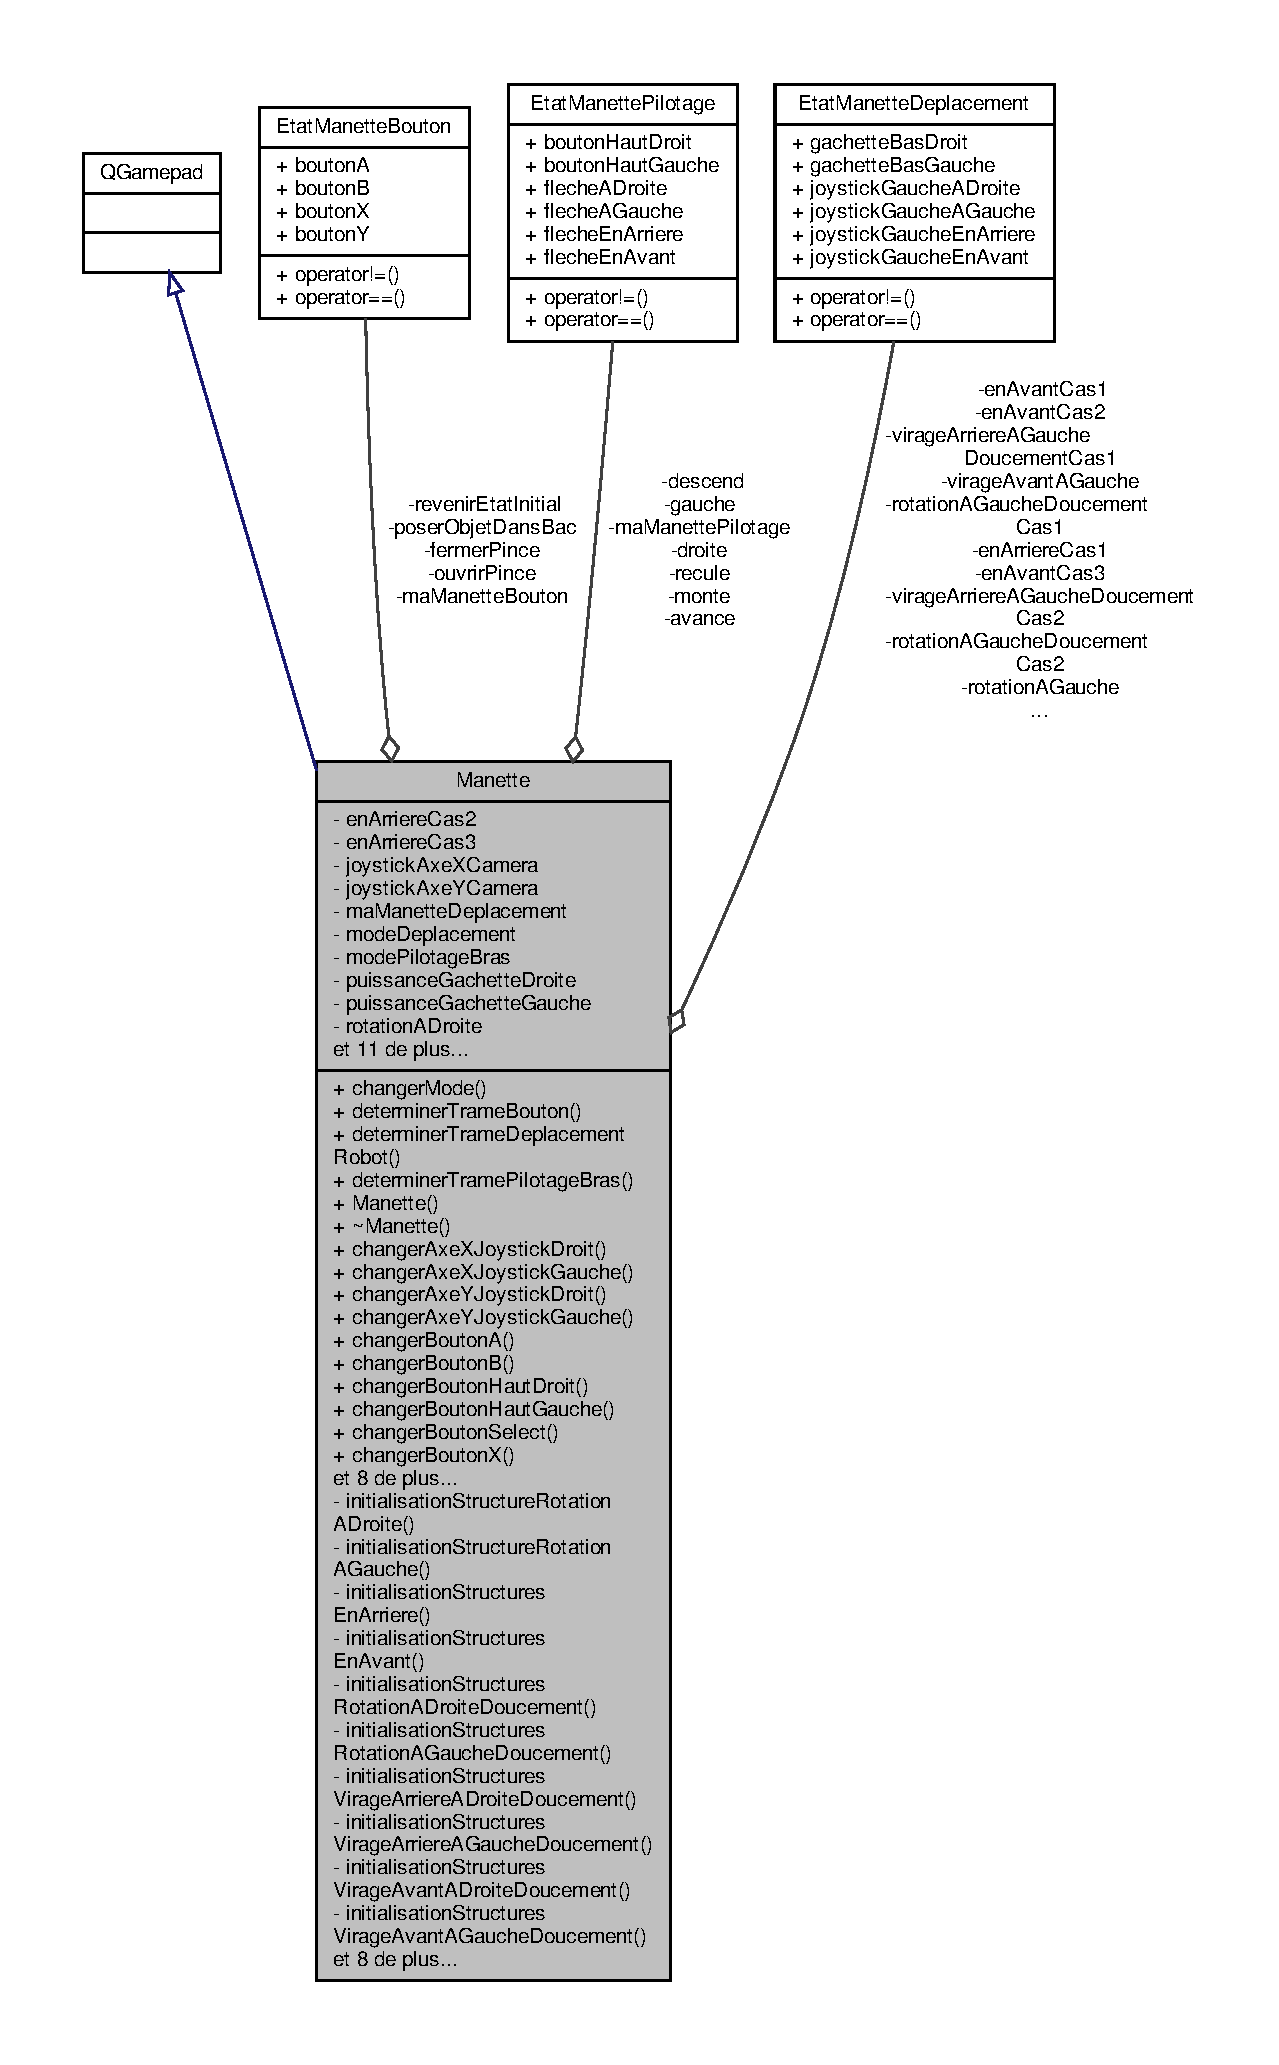
\includegraphics[height=550pt]{class_manette__coll__graph}
\end{center}
\end{figure}
\subsubsection*{Connecteurs publics}
\begin{DoxyCompactItemize}
\item 
void \hyperlink{class_manette_a37202e63cf8662fed5b3a2efc8eb99d1}{changer\+Axe\+X\+Joystick\+Droit} (double valeur)
\begin{DoxyCompactList}\small\item\em change l\textquotesingle{}etat de l\textquotesingle{}attribut joystick\+Axe\+X\+Camera en fonction du signe de \char`\"{}valeur\char`\"{} \end{DoxyCompactList}\item 
void \hyperlink{class_manette_a82a0d2535dd1dd9ea4021aa1fe71b1bc}{changer\+Axe\+X\+Joystick\+Gauche} (double valeur)
\begin{DoxyCompactList}\small\item\em change l\textquotesingle{}etat des attributs joystick\+Gauche\+A\+Gauche et joystick\+Gauche\+A\+Droite en fonction du signe de \char`\"{}valeur\char`\"{} \end{DoxyCompactList}\item 
void \hyperlink{class_manette_aaedc46e870b2731a79c5497296dba469}{changer\+Axe\+Y\+Joystick\+Droit} (double valeur)
\begin{DoxyCompactList}\small\item\em change l\textquotesingle{}etat de l\textquotesingle{}attribut joystick\+Axe\+Y\+Camera en fonction du signe de \char`\"{}valeur\char`\"{} \end{DoxyCompactList}\item 
void \hyperlink{class_manette_a6fd30466571a96d9789c54c8e8104ab2}{changer\+Axe\+Y\+Joystick\+Gauche} (double valeur)
\begin{DoxyCompactList}\small\item\em change l\textquotesingle{}etat des attributs joystick\+Gauche\+En\+Avant et joystick\+Gauche\+En\+Arriere en fonction du signe de \char`\"{}valeur\char`\"{} \end{DoxyCompactList}\item 
void \hyperlink{class_manette_aadf275d6bac238d48f8879d264bbc868}{changer\+BoutonA} (bool)
\begin{DoxyCompactList}\small\item\em change l\textquotesingle{}état du membre boutonA \end{DoxyCompactList}\item 
void \hyperlink{class_manette_af38f60c4bfa3f76da9c4598b0b144fd6}{changer\+BoutonB} (bool)
\begin{DoxyCompactList}\small\item\em change l\textquotesingle{}état du membre boutonB \end{DoxyCompactList}\item 
void \hyperlink{class_manette_a039b73883b0649e1bbaa7f7b3dff43f8}{changer\+Bouton\+Haut\+Droit} (bool etat)
\begin{DoxyCompactList}\small\item\em change l\textquotesingle{}etat des attributs bouton\+Haut\+Droit \end{DoxyCompactList}\item 
void \hyperlink{class_manette_a739830941c396dabb7c57862a1880a34}{changer\+Bouton\+Haut\+Gauche} (bool etat)
\begin{DoxyCompactList}\small\item\em change l\textquotesingle{}etat des attributs bouton\+Haut\+Gauche \end{DoxyCompactList}\item 
void \hyperlink{class_manette_a37710e94b9d871a577740daf13cb571b}{changer\+Bouton\+Select} (bool etat)
\begin{DoxyCompactList}\small\item\em change l\textquotesingle{}etat des attributs mode\+Deplacement mode\+Pilotage\+Bras en fonction de \char`\"{}etat\char`\"{} \end{DoxyCompactList}\item 
void \hyperlink{class_manette_a5d9f34f3ec334fa3880d93175f0df152}{changer\+BoutonX} (bool)
\begin{DoxyCompactList}\small\item\em change l\textquotesingle{}état du membre boutonX \end{DoxyCompactList}\item 
void \hyperlink{class_manette_a070a7551299aad2db041591004d2bc60}{changer\+BoutonY} (bool)
\begin{DoxyCompactList}\small\item\em change l\textquotesingle{}état du membre boutonY \end{DoxyCompactList}\item 
void \hyperlink{class_manette_abb0ab6adafd0785d1fef58481005ac41}{changer\+Fleche\+A\+Droite} (bool etat)
\begin{DoxyCompactList}\small\item\em change l\textquotesingle{}etat de l\textquotesingle{}attribut fleche\+A\+Droite en fonction de \char`\"{}etat\char`\"{} \end{DoxyCompactList}\item 
void \hyperlink{class_manette_ad4a00c510c7f6beb882d1e1d323346ae}{changer\+Fleche\+A\+Gauche} (bool etat)
\begin{DoxyCompactList}\small\item\em change l\textquotesingle{}etat de l\textquotesingle{}attribut fleche\+A\+Gauche en fonction de \char`\"{}valeur\char`\"{} \end{DoxyCompactList}\item 
void \hyperlink{class_manette_a6e83727ee7bf7b3276b86d08b1c8d4d5}{changer\+Fleche\+En\+Arriere} (bool etat)
\begin{DoxyCompactList}\small\item\em change l\textquotesingle{}etat de l\textquotesingle{}attribut fleche\+En\+Arriere en fonction de \char`\"{}valeur\char`\"{} \end{DoxyCompactList}\item 
void \hyperlink{class_manette_aec3aca0f38959daec78db1f97f79c2d6}{changer\+Fleche\+En\+Avant} (bool etat)
\begin{DoxyCompactList}\small\item\em change l\textquotesingle{}etat de l\textquotesingle{}attribut fleche\+En\+Avant en fonction de \char`\"{}valeur\char`\"{} \end{DoxyCompactList}\item 
void \hyperlink{class_manette_aa3540dc97fd85153baf80b9e06e8565f}{changer\+Gachette\+Bas\+Droit} (double valeur)
\begin{DoxyCompactList}\small\item\em change l\textquotesingle{}etat des attributs gachette\+Bas\+Droit et puissance en fonction de \char`\"{}valeur\char`\"{} \end{DoxyCompactList}\item 
void \hyperlink{class_manette_a858088ed0eb2259fcb2f3df390e950c9}{changer\+Gachette\+Bas\+Gauche} (double valeur)
\begin{DoxyCompactList}\small\item\em change l\textquotesingle{}etat des attributs gachette\+Bas\+Gauche et puissance en fonction de \char`\"{}valeur\char`\"{} \end{DoxyCompactList}\item 
void \hyperlink{class_manette_a7345a7c5bfdc566119f7db7358584b6c}{fermer\+Application} (bool etat)
\begin{DoxyCompactList}\small\item\em ferme l\textquotesingle{}application \end{DoxyCompactList}\end{DoxyCompactItemize}
\subsubsection*{Signaux}
\begin{DoxyCompactItemize}
\item 
void \hyperlink{class_manette_a4151ee98538d58d2dde6c8027e9ef512}{creation\+Trame\+Deplacement} (char deplacement\+AxeX, int puissance, char deplacement\+AxeY)
\begin{DoxyCompactList}\small\item\em Envoye des élément de la trame pour la création de la trame de déplacement. \end{DoxyCompactList}\item 
void \hyperlink{class_manette_ad28d8f539df6b73805ae94e9bbd827ec}{creation\+Trame\+Ordre} (Q\+String ordre)
\begin{DoxyCompactList}\small\item\em Envoye des élément de la trame pour la création de la trame des ordres. \end{DoxyCompactList}\item 
void \hyperlink{class_manette_a39de9cbde743771debc15501f8f8c154}{creation\+Trame\+Pilotage} (Q\+String direction)
\begin{DoxyCompactList}\small\item\em Envoye des élément de la trame pour la création de la trame de pilotage. \end{DoxyCompactList}\item 
void \hyperlink{class_manette_a16cb602cf7001f78b115f395fad47586}{creation\+Trame\+Pince} (Q\+String mouvement\+Pince)
\begin{DoxyCompactList}\small\item\em Envoye des élément de la trame pour la création de la trame d\textquotesingle{}ouverture et fermeture de la pince. \end{DoxyCompactList}\item 
void \hyperlink{class_manette_a229a449e851b5f716778d19c5cf2ba49}{nouvelle\+Trame\+Camera} (Q\+String axeY, Q\+String axeX)
\begin{DoxyCompactList}\small\item\em Nouvelle trame de commande de la caméra disponible. \end{DoxyCompactList}\item 
void \hyperlink{class_manette_a34d2a8b73a0913ef361d64f60e5d0eac}{prendre\+Photo} ()
\begin{DoxyCompactList}\small\item\em Envoi un signal indiquant que le bouton photo est pressé \end{DoxyCompactList}\end{DoxyCompactItemize}
\subsubsection*{Fonctions membres publiques}
\begin{DoxyCompactItemize}
\item 
void \hyperlink{class_manette_a202faf093876b9e95cfc316b552c59c3}{changer\+Mode} ()
\begin{DoxyCompactList}\small\item\em Change de mode en fonction du bouton S\+E\+L\+E\+CT. \end{DoxyCompactList}\item 
void \hyperlink{class_manette_a3fb9d1245400b6bb6379fbb63a8099ba}{determiner\+Trame\+Bouton} ()
\begin{DoxyCompactList}\small\item\em Verifie l\textquotesingle{}etat de la manette et creer la trame correspondante. \end{DoxyCompactList}\item 
void \hyperlink{class_manette_a97a50caac68954a229c7e9461e7f4232}{determiner\+Trame\+Deplacement\+Robot} ()
\begin{DoxyCompactList}\small\item\em Verifie l\textquotesingle{}etat de la manette et creer la trame correspondante. \end{DoxyCompactList}\item 
void \hyperlink{class_manette_ab5eb6972f366aa7527b2b27da5539638}{determiner\+Trame\+Pilotage\+Bras} ()
\begin{DoxyCompactList}\small\item\em Verifie l\textquotesingle{}etat de la manette et creer la trame correspondante. \end{DoxyCompactList}\item 
\hyperlink{class_manette_aaeb630a14bd4905666146dca3253827b}{Manette} (int device\+Id)
\begin{DoxyCompactList}\small\item\em Contructeur de la classe \hyperlink{class_manette}{Manette}. \end{DoxyCompactList}\item 
\hyperlink{class_manette_a86a0cab49599b27d86c2e77f13fa54a2}{$\sim$\+Manette} ()
\begin{DoxyCompactList}\small\item\em Destructeur de la classe \hyperlink{class_manette}{Manette}. \end{DoxyCompactList}\end{DoxyCompactItemize}
\subsubsection*{Fonctions membres privées}
\begin{DoxyCompactItemize}
\item 
void \hyperlink{class_manette_a34e37141425dd6d62bcb5954312705c9}{initialisation\+Structure\+Rotation\+A\+Droite} ()
\begin{DoxyCompactList}\small\item\em Initialise les états de la structures rotation\+A\+Droite. \end{DoxyCompactList}\item 
void \hyperlink{class_manette_a9c1348e7b4c4cc071c9b8bac79f0eeab}{initialisation\+Structure\+Rotation\+A\+Gauche} ()
\begin{DoxyCompactList}\small\item\em Initialise les états de la structures rotation\+A\+Gauche. \end{DoxyCompactList}\item 
void \hyperlink{class_manette_ae4379b4f09192b83219de5aaa548fda0}{initialisation\+Structures\+En\+Arriere} ()
\begin{DoxyCompactList}\small\item\em Initialise les états de la structures en\+Arriere. \end{DoxyCompactList}\item 
void \hyperlink{class_manette_afd5504555886e0abf89347b4f8d57fe0}{initialisation\+Structures\+En\+Avant} ()
\begin{DoxyCompactList}\small\item\em Initialise les états de la structures en\+Avant. \end{DoxyCompactList}\item 
void \hyperlink{class_manette_aba0348198bad2dff52fe71684d73c2df}{initialisation\+Structures\+Rotation\+A\+Droite\+Doucement} ()
\begin{DoxyCompactList}\small\item\em Initialise les états de la structures rotation\+A\+Droite\+Doucement. \end{DoxyCompactList}\item 
void \hyperlink{class_manette_a35242782669d6d2cf88f2b5dbd9b0b73}{initialisation\+Structures\+Rotation\+A\+Gauche\+Doucement} ()
\begin{DoxyCompactList}\small\item\em Initialise les états de la structures rotation\+A\+Gauche\+Doucement. \end{DoxyCompactList}\item 
void \hyperlink{class_manette_a118d9481c3eecb4dcc58f8798893fa85}{initialisation\+Structures\+Virage\+Arriere\+A\+Droite\+Doucement} ()
\begin{DoxyCompactList}\small\item\em Initialise les états de la structures virage\+Arriere\+A\+Droite\+Doucement. \end{DoxyCompactList}\item 
void \hyperlink{class_manette_a345202d80c6b1370284103878e690363}{initialisation\+Structures\+Virage\+Arriere\+A\+Gauche\+Doucement} ()
\begin{DoxyCompactList}\small\item\em Initialise les états de la structures virage\+Arriere\+A\+Gauche\+Doucement. \end{DoxyCompactList}\item 
void \hyperlink{class_manette_ac77d5caae62d9248edd5e26f15176f34}{initialisation\+Structures\+Virage\+Avant\+A\+Droite\+Doucement} ()
\begin{DoxyCompactList}\small\item\em Initialise les états de la structures virage\+Avant\+A\+Droite. \end{DoxyCompactList}\item 
void \hyperlink{class_manette_ac01c5ff122f042497658f00d3df9e859}{initialisation\+Structures\+Virage\+Avant\+A\+Gauche\+Doucement} ()
\begin{DoxyCompactList}\small\item\em Initialise les états de la structures virage\+Avant\+A\+Gauche\+Doucement. \end{DoxyCompactList}\item 
void \hyperlink{class_manette_a9097a15ce44cb2535ce6e6099a8b2095}{initialisation\+Structure\+Virage\+Arriere\+A\+Droite} ()
\begin{DoxyCompactList}\small\item\em Initialise les états de la structures virage\+Arriere\+A\+Droite. \end{DoxyCompactList}\item 
void \hyperlink{class_manette_ad1d146fe52ff367fd2a7fe3c94c165e4}{initialisation\+Structure\+Virage\+Arriere\+A\+Gauche} ()
\begin{DoxyCompactList}\small\item\em Initialise les états de la structures virage\+Arriere\+A\+Gauche. \end{DoxyCompactList}\item 
void \hyperlink{class_manette_ad41918ccfeee9d80146a74678173cee8}{initialisation\+Structure\+Virage\+Avant\+A\+Droite} ()
\begin{DoxyCompactList}\small\item\em Initialise les états de la structures. \end{DoxyCompactList}\item 
void \hyperlink{class_manette_aa02a2dfa49318e1043b52dd103fa1795}{initialisation\+Structure\+Virage\+Avant\+A\+Gauche} ()
\begin{DoxyCompactList}\small\item\em Initialise les états de la structures virage\+Avant\+A\+Gauche. \end{DoxyCompactList}\item 
void \hyperlink{class_manette_a21ebb19837250342e4859ba7dc5f03cc}{initialiser\+Etat\+Bouton} ()
\begin{DoxyCompactList}\small\item\em Initialise les états des structures Etat\+Bouton. \end{DoxyCompactList}\item 
void \hyperlink{class_manette_afd722561b4cc62304e81a8e41c820bb8}{initialiser\+Etats} ()
\begin{DoxyCompactList}\small\item\em Initialise les états de la manette. \end{DoxyCompactList}\item 
void \hyperlink{class_manette_a9888b04a784ceda912a35b6eb30ae84a}{initialiser\+Types\+Deplacement} ()
\begin{DoxyCompactList}\small\item\em Initialise les états de la manette pour le déplacement. \end{DoxyCompactList}\item 
void \hyperlink{class_manette_ab20afdb190b24126e54d4f80af0bf310}{initialiser\+Types\+Pilotage} ()
\begin{DoxyCompactList}\small\item\em Initialise les états de la manette pour le pilotage. \end{DoxyCompactList}\end{DoxyCompactItemize}
\subsubsection*{Attributs privés}
\begin{DoxyCompactItemize}
\item 
\hyperlink{struct_etat_manette_pilotage}{Etat\+Manette\+Pilotage} \hyperlink{class_manette_a6ff181eab8c2206ca3d40bf5112e72ec}{avance}
\begin{DoxyCompactList}\small\item\em Structure définissant l\textquotesingle{}état des bouton de la manette pour avancer. \end{DoxyCompactList}\item 
\hyperlink{struct_etat_manette_pilotage}{Etat\+Manette\+Pilotage} \hyperlink{class_manette_a95e7f41f1e15f01d7530062801817304}{descend}
\begin{DoxyCompactList}\small\item\em Structure définissant l\textquotesingle{}état des bouton de la manette pour descendre. \end{DoxyCompactList}\item 
\hyperlink{struct_etat_manette_pilotage}{Etat\+Manette\+Pilotage} \hyperlink{class_manette_a40a2dc8420742b04c3eee14e477992b1}{droite}
\begin{DoxyCompactList}\small\item\em Structure définissant l\textquotesingle{}état des bouton de la manette pour aller à droite. \end{DoxyCompactList}\item 
\hyperlink{struct_etat_manette_deplacement}{Etat\+Manette\+Deplacement} \hyperlink{class_manette_a915c1867ed0f8f9be3a1bf5d87c23813}{en\+Arriere\+Cas1}
\begin{DoxyCompactList}\small\item\em Structure définissant l\textquotesingle{}état des bouton de la manette en mode deplacement du robot pour reculer. \end{DoxyCompactList}\item 
\hyperlink{struct_etat_manette_deplacement}{Etat\+Manette\+Deplacement} \hyperlink{class_manette_aa620cef4ea733aa3b9dee18377aee140}{en\+Arriere\+Cas2}
\begin{DoxyCompactList}\small\item\em Structure définissant l\textquotesingle{}état des bouton de la manette en mode deplacement du robot pour reculer. \end{DoxyCompactList}\item 
\hyperlink{struct_etat_manette_deplacement}{Etat\+Manette\+Deplacement} \hyperlink{class_manette_a2dfc47df38251abd34a495005eae6572}{en\+Arriere\+Cas3}
\begin{DoxyCompactList}\small\item\em Structure définissant l\textquotesingle{}état des bouton de la manette en mode deplacement du robot pour reculer. \end{DoxyCompactList}\item 
\hyperlink{struct_etat_manette_deplacement}{Etat\+Manette\+Deplacement} \hyperlink{class_manette_ad6d8777e6a4885b343389a04174cf1c9}{en\+Avant\+Cas1}
\begin{DoxyCompactList}\small\item\em Structure définissant l\textquotesingle{}état des bouton de la manette en mode deplacement du robot pour avancer. \end{DoxyCompactList}\item 
\hyperlink{struct_etat_manette_deplacement}{Etat\+Manette\+Deplacement} \hyperlink{class_manette_a37e31078db889bbf8202b7d8cb9c5947}{en\+Avant\+Cas2}
\begin{DoxyCompactList}\small\item\em Structure définissant l\textquotesingle{}état des bouton de la manette en mode deplacement du robot pour avancer. \end{DoxyCompactList}\item 
\hyperlink{struct_etat_manette_deplacement}{Etat\+Manette\+Deplacement} \hyperlink{class_manette_a4546e6f56bac4a9e99a92539a68f3c5c}{en\+Avant\+Cas3}
\begin{DoxyCompactList}\small\item\em Structure définissant l\textquotesingle{}état des bouton de la manette en mode deplacement du robot pour avancer. \end{DoxyCompactList}\item 
\hyperlink{struct_etat_manette_bouton}{Etat\+Manette\+Bouton} \hyperlink{class_manette_a32adcccdddf35a04970b8b3b12462c00}{fermer\+Pince}
\begin{DoxyCompactList}\small\item\em Structure définissant l\textquotesingle{}etat des bouton A, B, X, Y de la manette pour fermer la pince. \end{DoxyCompactList}\item 
\hyperlink{struct_etat_manette_pilotage}{Etat\+Manette\+Pilotage} \hyperlink{class_manette_acc72f831540b93ac3a265d35d005c4fa}{gauche}
\begin{DoxyCompactList}\small\item\em Structure définissant l\textquotesingle{}état des bouton de la manette pour aller à gauche. \end{DoxyCompactList}\item 
Q\+String \hyperlink{class_manette_a0ca05a5c08455e74c8d944b96d8124a6}{joystick\+Axe\+X\+Camera}
\begin{DoxyCompactList}\small\item\em Attribut contenant l\textquotesingle{}etat actuel du joystick droite sur l\textquotesingle{}axe des x. \end{DoxyCompactList}\item 
Q\+String \hyperlink{class_manette_ab635d71c9e829d8950b9bbd13b9cdb01}{joystick\+Axe\+Y\+Camera}
\begin{DoxyCompactList}\small\item\em Attribut contenant l\textquotesingle{}etat actuel du joystick droite sur l\textquotesingle{}axe des y. \end{DoxyCompactList}\item 
\hyperlink{struct_etat_manette_bouton}{Etat\+Manette\+Bouton} \hyperlink{class_manette_ae69fd9baa0dad8a960fa93611b6a185f}{ma\+Manette\+Bouton}
\begin{DoxyCompactList}\small\item\em Structure définissant l\textquotesingle{}etat des bouton A, B, X, Y de la manette. \end{DoxyCompactList}\item 
\hyperlink{struct_etat_manette_deplacement}{Etat\+Manette\+Deplacement} \hyperlink{class_manette_af3d0f304c4c33e02bdf34fc99aa4dbff}{ma\+Manette\+Deplacement}
\begin{DoxyCompactList}\small\item\em Structure définissant l\textquotesingle{}état des bouton de la manette en mode deplacement du robot. \end{DoxyCompactList}\item 
\hyperlink{struct_etat_manette_pilotage}{Etat\+Manette\+Pilotage} \hyperlink{class_manette_aeb3e02eaeaec4c656f78ed8fc6dae342}{ma\+Manette\+Pilotage}
\begin{DoxyCompactList}\small\item\em Structure définissant l\textquotesingle{}état des bouton de la manette en mode pilotage du bras. \end{DoxyCompactList}\item 
bool \hyperlink{class_manette_a4dc6231c8cc65fac03f59d323fa9a038}{mode\+Deplacement}
\begin{DoxyCompactList}\small\item\em Attribut définissant l\textquotesingle{}état du mode de déplacement. \end{DoxyCompactList}\item 
bool \hyperlink{class_manette_acc2cd9afa45328c0da5c580e5c1a67db}{mode\+Pilotage\+Bras}
\begin{DoxyCompactList}\small\item\em Attribut définissant l\textquotesingle{}état du mode pilotage du bras articulé \end{DoxyCompactList}\item 
\hyperlink{struct_etat_manette_pilotage}{Etat\+Manette\+Pilotage} \hyperlink{class_manette_a63d9a39ea238e105d7491b87f0a3f87d}{monte}
\begin{DoxyCompactList}\small\item\em Structure définissant l\textquotesingle{}état des bouton de la manette pour monter. \end{DoxyCompactList}\item 
\hyperlink{struct_etat_manette_bouton}{Etat\+Manette\+Bouton} \hyperlink{class_manette_a066eacf19e615fd72690477c043e3703}{ouvrir\+Pince}
\begin{DoxyCompactList}\small\item\em Structure définissant l\textquotesingle{}etat des bouton A, B, X, Y de la manette pour ouvrir la pince. \end{DoxyCompactList}\item 
\hyperlink{struct_etat_manette_bouton}{Etat\+Manette\+Bouton} \hyperlink{class_manette_a93fc38a8ca8fbb1cc57cedbab059c56f}{poser\+Objet\+Dans\+Bac}
\begin{DoxyCompactList}\small\item\em Structure définissant l\textquotesingle{}etat des bouton A, B, X, Y de la manette pour poser l\textquotesingle{}objet dans le bac. \end{DoxyCompactList}\item 
int \hyperlink{class_manette_a135a3a6f567bbeeefd69b3a020f9f040}{puissance\+Gachette\+Droite}
\begin{DoxyCompactList}\small\item\em Attribut définissant la valeur de la puissance de la gachette droite. \end{DoxyCompactList}\item 
int \hyperlink{class_manette_ab777328c9b35454ab45ed5e0b0a5f234}{puissance\+Gachette\+Gauche}
\begin{DoxyCompactList}\small\item\em Attribut définissant la valeur de la puissance de la gachette gauche. \end{DoxyCompactList}\item 
\hyperlink{struct_etat_manette_pilotage}{Etat\+Manette\+Pilotage} \hyperlink{class_manette_a5ed3a0ab27f98cd11ecafe5f5b94e7e5}{recule}
\begin{DoxyCompactList}\small\item\em Structure définissant l\textquotesingle{}état des bouton de la manette pour reculer. \end{DoxyCompactList}\item 
\hyperlink{struct_etat_manette_bouton}{Etat\+Manette\+Bouton} \hyperlink{class_manette_a4c0e9611f08e363feb0a24f8c9d258f2}{revenir\+Etat\+Initial}
\begin{DoxyCompactList}\small\item\em Structure définissant l\textquotesingle{}etat des bouton A, B, X, Y de la manette pour revenir à l\textquotesingle{}etat initiale du bras. \end{DoxyCompactList}\item 
\hyperlink{struct_etat_manette_deplacement}{Etat\+Manette\+Deplacement} \hyperlink{class_manette_abeff301c65d7faeb68e7d38b8f0b5122}{rotation\+A\+Droite}
\begin{DoxyCompactList}\small\item\em Structure définissant l\textquotesingle{}état des bouton de la manette en mode deplacement du robot pour tourner à droite. \end{DoxyCompactList}\item 
\hyperlink{struct_etat_manette_deplacement}{Etat\+Manette\+Deplacement} \hyperlink{class_manette_ac7bf8fa21acad7d4afe9e73c62c224a9}{rotation\+A\+Droite\+Doucement\+Cas1}
\begin{DoxyCompactList}\small\item\em Structure définissant l\textquotesingle{}état des bouton de la manette en mode deplacement du robot pour tourner à droite doucement. \end{DoxyCompactList}\item 
\hyperlink{struct_etat_manette_deplacement}{Etat\+Manette\+Deplacement} \hyperlink{class_manette_a1ae7c87ab4c27fec817e7b02de9e546b}{rotation\+A\+Droite\+Doucement\+Cas2}
\begin{DoxyCompactList}\small\item\em Structure définissant l\textquotesingle{}état des bouton de la manette en mode deplacement du robot pour tourner à droite doucement. \end{DoxyCompactList}\item 
\hyperlink{struct_etat_manette_deplacement}{Etat\+Manette\+Deplacement} \hyperlink{class_manette_a3aa7b857df1a364d70f1626f2f517056}{rotation\+A\+Gauche}
\begin{DoxyCompactList}\small\item\em Structure définissant l\textquotesingle{}état des bouton de la manette en mode deplacement du robot pour tourner à gauche. \end{DoxyCompactList}\item 
\hyperlink{struct_etat_manette_deplacement}{Etat\+Manette\+Deplacement} \hyperlink{class_manette_ac24e87d64418d5667a378b2f508a0759}{rotation\+A\+Gauche\+Doucement\+Cas1}
\begin{DoxyCompactList}\small\item\em Structure définissant l\textquotesingle{}état des bouton de la manette en mode deplacement du robot pour tourner à gauche doucement. \end{DoxyCompactList}\item 
\hyperlink{struct_etat_manette_deplacement}{Etat\+Manette\+Deplacement} \hyperlink{class_manette_a21fa44eaadd677f97cdc876da8fe3143}{rotation\+A\+Gauche\+Doucement\+Cas2}
\begin{DoxyCompactList}\small\item\em Structure définissant l\textquotesingle{}état des bouton de la manette en mode deplacement du robot pour tourner à gauche doucement. \end{DoxyCompactList}\item 
\hyperlink{struct_etat_manette_deplacement}{Etat\+Manette\+Deplacement} \hyperlink{class_manette_a6df334aec9f621e7394e9f398221fe9e}{virage\+Arriere\+A\+Droite}
\begin{DoxyCompactList}\small\item\em Structure définissant l\textquotesingle{}état des bouton de la manette en mode deplacement du robot pour reculer et tourner à droite. \end{DoxyCompactList}\item 
\hyperlink{struct_etat_manette_deplacement}{Etat\+Manette\+Deplacement} \hyperlink{class_manette_a2dddb8a8a6f75abc15ddf58025b98ecc}{virage\+Arriere\+A\+Droite\+Doucement\+Cas1}
\begin{DoxyCompactList}\small\item\em Structure définissant l\textquotesingle{}état des bouton de la manette en mode deplacement du robot pour reculer et tourner à droite doucement. \end{DoxyCompactList}\item 
\hyperlink{struct_etat_manette_deplacement}{Etat\+Manette\+Deplacement} \hyperlink{class_manette_a609f10f48e39eafac800eb232272f0cb}{virage\+Arriere\+A\+Droite\+Doucement\+Cas2}
\begin{DoxyCompactList}\small\item\em Structure définissant l\textquotesingle{}état des bouton de la manette en mode deplacement du robot pour reculer et tourner à droite doucement. \end{DoxyCompactList}\item 
\hyperlink{struct_etat_manette_deplacement}{Etat\+Manette\+Deplacement} \hyperlink{class_manette_a92a64ea372e58825097e049694e838a1}{virage\+Arriere\+A\+Gauche}
\begin{DoxyCompactList}\small\item\em Structure définissant l\textquotesingle{}état des bouton de la manette en mode deplacement du robot pour reculer et tourner à gauche. \end{DoxyCompactList}\item 
\hyperlink{struct_etat_manette_deplacement}{Etat\+Manette\+Deplacement} \hyperlink{class_manette_a984a465aac5dda20091f561339dd351d}{virage\+Arriere\+A\+Gauche\+Doucement\+Cas1}
\begin{DoxyCompactList}\small\item\em Structure définissant l\textquotesingle{}état des bouton de la manette en mode deplacement du robot pour reculer et tourner à gauche doucement. \end{DoxyCompactList}\item 
\hyperlink{struct_etat_manette_deplacement}{Etat\+Manette\+Deplacement} \hyperlink{class_manette_ac509477cff14d1ab9562c03e9db833f8}{virage\+Arriere\+A\+Gauche\+Doucement\+Cas2}
\begin{DoxyCompactList}\small\item\em Structure définissant l\textquotesingle{}état des bouton de la manette en mode deplacement du robot pour reculer et tourner à gauche doucement. \end{DoxyCompactList}\item 
\hyperlink{struct_etat_manette_deplacement}{Etat\+Manette\+Deplacement} \hyperlink{class_manette_a91afd62402f690f74a7e351c9aa8f6ec}{virage\+Avant\+A\+Droite}
\begin{DoxyCompactList}\small\item\em Structure définissant l\textquotesingle{}état des bouton de la manette en mode deplacement du robot pour avancer et tourner à droite. \end{DoxyCompactList}\item 
\hyperlink{struct_etat_manette_deplacement}{Etat\+Manette\+Deplacement} \hyperlink{class_manette_ad4aeabac283607d7d37823aabd4c5e0f}{virage\+Avant\+A\+Droite\+Doucement\+Cas1}
\begin{DoxyCompactList}\small\item\em Structure définissant l\textquotesingle{}état des bouton de la manette en mode deplacement du robot pour avancer et tourner à droite doucement. \end{DoxyCompactList}\item 
\hyperlink{struct_etat_manette_deplacement}{Etat\+Manette\+Deplacement} \hyperlink{class_manette_a6b8d8fd853462fa182a37122b692db90}{virage\+Avant\+A\+Droite\+Doucement\+Cas2}
\begin{DoxyCompactList}\small\item\em Structure définissant l\textquotesingle{}état des bouton de la manette en mode deplacement du robot pour avancer et tourner à droite doucement. \end{DoxyCompactList}\item 
\hyperlink{struct_etat_manette_deplacement}{Etat\+Manette\+Deplacement} \hyperlink{class_manette_a3f44a6304ed3b17176636bad8f2220db}{virage\+Avant\+A\+Gauche}
\begin{DoxyCompactList}\small\item\em Structure définissant l\textquotesingle{}état des bouton de la manette en mode deplacement du robot pour avancer et tourner à gauche. \end{DoxyCompactList}\item 
\hyperlink{struct_etat_manette_deplacement}{Etat\+Manette\+Deplacement} \hyperlink{class_manette_a0fe6d52d8ca1060a2a3c534847824c09}{virage\+Avant\+A\+Gauche\+Doucement\+Cas1}
\begin{DoxyCompactList}\small\item\em Structure définissant l\textquotesingle{}état des bouton de la manette en mode deplacement du robot pour avancer et tourner à gauche doucement. \end{DoxyCompactList}\item 
\hyperlink{struct_etat_manette_deplacement}{Etat\+Manette\+Deplacement} \hyperlink{class_manette_a575018c439de0fd1e8cf7be5907ca60d}{virage\+Avant\+A\+Gauche\+Doucement\+Cas2}
\begin{DoxyCompactList}\small\item\em Structure définissant l\textquotesingle{}état des bouton de la manette en mode deplacement du robot pour avancer et tourner à gauche doucement. \end{DoxyCompactList}\end{DoxyCompactItemize}


\subsubsection{Description détaillée}
Classe permettant une communication entre le rov et la manette. 

Définition à la ligne \hyperlink{manette_8h_source_l00210}{210} du fichier \hyperlink{manette_8h_source}{manette.\+h}.



\subsubsection{Documentation des constructeurs et destructeur}
\mbox{\Hypertarget{class_manette_aaeb630a14bd4905666146dca3253827b}\label{class_manette_aaeb630a14bd4905666146dca3253827b}} 
\index{Manette@{Manette}!Manette@{Manette}}
\index{Manette@{Manette}!Manette@{Manette}}
\paragraph{\texorpdfstring{Manette()}{Manette()}}
{\footnotesize\ttfamily Manette\+::\+Manette (\begin{DoxyParamCaption}\item[{int}]{device\+Id }\end{DoxyParamCaption})\hspace{0.3cm}{\ttfamily [explicit]}}



Contructeur de la classe \hyperlink{class_manette}{Manette}. 


\begin{DoxyParams}{Paramètres}
{\em device\+Id} & \\
\hline
\end{DoxyParams}


Définition à la ligne \hyperlink{manette_8cpp_source_l00009}{9} du fichier \hyperlink{manette_8cpp_source}{manette.\+cpp}.



Références \hyperlink{manette_8cpp_source_l00313}{initialiser\+Etat\+Bouton()}, \hyperlink{manette_8cpp_source_l00023}{initialiser\+Etats()}, \hyperlink{manette_8cpp_source_l00085}{initialiser\+Types\+Deplacement()}, et \hyperlink{manette_8cpp_source_l00040}{initialiser\+Types\+Pilotage()}.


\begin{DoxyCode}
00009                              : \hyperlink{class_q_gamepad}{QGamepad}(deviceID), \hyperlink{class_manette_a4dc6231c8cc65fac03f59d323fa9a038}{modeDeplacement}(\textcolor{keyword}{true}), 
      \hyperlink{class_manette_acc2cd9afa45328c0da5c580e5c1a67db}{modePilotageBras}(\textcolor{keyword}{false}), \hyperlink{class_manette_a135a3a6f567bbeeefd69b3a020f9f040}{puissanceGachetteDroite}(0), 
      \hyperlink{class_manette_ab777328c9b35454ab45ed5e0b0a5f234}{puissanceGachetteGauche}(0), \hyperlink{class_manette_a0ca05a5c08455e74c8d944b96d8124a6}{joystickAxeXCamera}(\textcolor{stringliteral}{"0"}), 
      \hyperlink{class_manette_ab635d71c9e829d8950b9bbd13b9cdb01}{joystickAxeYCamera}(\textcolor{stringliteral}{"0"})
00010 \{
00011     qDebug() << Q\_FUNC\_INFO << \textcolor{keyword}{this};
00012     \hyperlink{class_manette_afd722561b4cc62304e81a8e41c820bb8}{initialiserEtats}();
00013     \hyperlink{class_manette_a21ebb19837250342e4859ba7dc5f03cc}{initialiserEtatBouton}();
00014     \hyperlink{class_manette_ab20afdb190b24126e54d4f80af0bf310}{initialiserTypesPilotage}();
00015     \hyperlink{class_manette_a9888b04a784ceda912a35b6eb30ae84a}{initialiserTypesDeplacement}();
00016 \}
\end{DoxyCode}
\mbox{\Hypertarget{class_manette_a86a0cab49599b27d86c2e77f13fa54a2}\label{class_manette_a86a0cab49599b27d86c2e77f13fa54a2}} 
\index{Manette@{Manette}!````~Manette@{$\sim$\+Manette}}
\index{````~Manette@{$\sim$\+Manette}!Manette@{Manette}}
\paragraph{\texorpdfstring{$\sim$\+Manette()}{~Manette()}}
{\footnotesize\ttfamily Manette\+::$\sim$\+Manette (\begin{DoxyParamCaption}{ }\end{DoxyParamCaption})}



Destructeur de la classe \hyperlink{class_manette}{Manette}. 



Définition à la ligne \hyperlink{manette_8cpp_source_l00018}{18} du fichier \hyperlink{manette_8cpp_source}{manette.\+cpp}.


\begin{DoxyCode}
00019 \{
00020     qDebug() << Q\_FUNC\_INFO << \textcolor{keyword}{this};
00021 \}
\end{DoxyCode}


\subsubsection{Documentation des fonctions membres}
\mbox{\Hypertarget{class_manette_a37202e63cf8662fed5b3a2efc8eb99d1}\label{class_manette_a37202e63cf8662fed5b3a2efc8eb99d1}} 
\index{Manette@{Manette}!changer\+Axe\+X\+Joystick\+Droit@{changer\+Axe\+X\+Joystick\+Droit}}
\index{changer\+Axe\+X\+Joystick\+Droit@{changer\+Axe\+X\+Joystick\+Droit}!Manette@{Manette}}
\paragraph{\texorpdfstring{changer\+Axe\+X\+Joystick\+Droit}{changerAxeXJoystickDroit}}
{\footnotesize\ttfamily void Manette\+::changer\+Axe\+X\+Joystick\+Droit (\begin{DoxyParamCaption}\item[{double}]{valeur }\end{DoxyParamCaption})\hspace{0.3cm}{\ttfamily [slot]}}



change l\textquotesingle{}etat de l\textquotesingle{}attribut joystick\+Axe\+X\+Camera en fonction du signe de \char`\"{}valeur\char`\"{} 


\begin{DoxyParams}{Paramètres}
{\em valeur} & \\
\hline
\end{DoxyParams}


Définition à la ligne \hyperlink{manette_8cpp_source_l00455}{455} du fichier \hyperlink{manette_8cpp_source}{manette.\+cpp}.



Références \hyperlink{manette_8h_source_l00257}{joystick\+Axe\+X\+Camera}, \hyperlink{manette_8h_source_l00258}{joystick\+Axe\+Y\+Camera}, \hyperlink{class_manette_a229a449e851b5f716778d19c5cf2ba49}{nouvelle\+Trame\+Camera()}, et \hyperlink{manette_8h_source_l00020}{T\+A\+U\+X\+\_\+\+V\+A\+L\+I\+D\+I\+T\+E\+\_\+\+J\+O\+Y\+S\+T\+I\+CK}.


\begin{DoxyCode}
00456 \{
00457     \textcolor{keywordflow}{if}(valeur >= \hyperlink{manette_8h_a1ae244fc787303cd46a9b684fb4b4056}{TAUX\_VALIDITE\_JOYSTICK})
00458         \hyperlink{class_manette_a0ca05a5c08455e74c8d944b96d8124a6}{joystickAxeXCamera} = \textcolor{stringliteral}{"D"};
00459     \textcolor{keywordflow}{else} \textcolor{keywordflow}{if}(valeur <= -\hyperlink{manette_8h_a1ae244fc787303cd46a9b684fb4b4056}{TAUX\_VALIDITE\_JOYSTICK})
00460         \hyperlink{class_manette_a0ca05a5c08455e74c8d944b96d8124a6}{joystickAxeXCamera} = \textcolor{stringliteral}{"G"};
00461     \textcolor{keywordflow}{else}
00462         \hyperlink{class_manette_a0ca05a5c08455e74c8d944b96d8124a6}{joystickAxeXCamera} = \textcolor{stringliteral}{"0"};
00463 
00464     emit \hyperlink{class_manette_a229a449e851b5f716778d19c5cf2ba49}{nouvelleTrameCamera}(\hyperlink{class_manette_a0ca05a5c08455e74c8d944b96d8124a6}{joystickAxeXCamera}, 
      \hyperlink{class_manette_ab635d71c9e829d8950b9bbd13b9cdb01}{joystickAxeYCamera});
00465 \}
\end{DoxyCode}
\mbox{\Hypertarget{class_manette_a82a0d2535dd1dd9ea4021aa1fe71b1bc}\label{class_manette_a82a0d2535dd1dd9ea4021aa1fe71b1bc}} 
\index{Manette@{Manette}!changer\+Axe\+X\+Joystick\+Gauche@{changer\+Axe\+X\+Joystick\+Gauche}}
\index{changer\+Axe\+X\+Joystick\+Gauche@{changer\+Axe\+X\+Joystick\+Gauche}!Manette@{Manette}}
\paragraph{\texorpdfstring{changer\+Axe\+X\+Joystick\+Gauche}{changerAxeXJoystickGauche}}
{\footnotesize\ttfamily void Manette\+::changer\+Axe\+X\+Joystick\+Gauche (\begin{DoxyParamCaption}\item[{double}]{valeur }\end{DoxyParamCaption})\hspace{0.3cm}{\ttfamily [slot]}}



change l\textquotesingle{}etat des attributs joystick\+Gauche\+A\+Gauche et joystick\+Gauche\+A\+Droite en fonction du signe de \char`\"{}valeur\char`\"{} 


\begin{DoxyParams}{Paramètres}
{\em valeur} & \\
\hline
\end{DoxyParams}


Définition à la ligne \hyperlink{manette_8cpp_source_l00421}{421} du fichier \hyperlink{manette_8cpp_source}{manette.\+cpp}.



Références \hyperlink{manette_8cpp_source_l00341}{determiner\+Trame\+Deplacement\+Robot()}, \hyperlink{manette_8h_source_l00183}{Etat\+Manette\+Deplacement\+::joystick\+Gauche\+A\+Droite}, \hyperlink{manette_8h_source_l00182}{Etat\+Manette\+Deplacement\+::joystick\+Gauche\+A\+Gauche}, \hyperlink{manette_8h_source_l00220}{ma\+Manette\+Deplacement}, \hyperlink{manette_8h_source_l00253}{mode\+Deplacement}, et \hyperlink{manette_8h_source_l00020}{T\+A\+U\+X\+\_\+\+V\+A\+L\+I\+D\+I\+T\+E\+\_\+\+J\+O\+Y\+S\+T\+I\+CK}.


\begin{DoxyCode}
00422 \{
00423     \textcolor{keywordflow}{if}(\hyperlink{class_manette_a4dc6231c8cc65fac03f59d323fa9a038}{modeDeplacement})
00424     \{
00425         \textcolor{keywordflow}{if}(valeur <= -\hyperlink{manette_8h_a1ae244fc787303cd46a9b684fb4b4056}{TAUX\_VALIDITE\_JOYSTICK})
00426             \hyperlink{class_manette_af3d0f304c4c33e02bdf34fc99aa4dbff}{maManetteDeplacement}.\hyperlink{struct_etat_manette_deplacement_af7e92a8d8f116e2bc4a5a95386f604e7}{joystickGaucheAGauche} = \textcolor{keyword}{true};
00427         \textcolor{keywordflow}{else} \textcolor{keywordflow}{if}(valeur >= \hyperlink{manette_8h_a1ae244fc787303cd46a9b684fb4b4056}{TAUX\_VALIDITE\_JOYSTICK})
00428             \hyperlink{class_manette_af3d0f304c4c33e02bdf34fc99aa4dbff}{maManetteDeplacement}.\hyperlink{struct_etat_manette_deplacement_a8fa93da5af430ac00ffd4ee8b76987a2}{joystickGaucheADroite} = \textcolor{keyword}{true};
00429         \textcolor{keywordflow}{else} \textcolor{keywordflow}{if}(valeur > -\hyperlink{manette_8h_a1ae244fc787303cd46a9b684fb4b4056}{TAUX\_VALIDITE\_JOYSTICK} && valeur < 
      \hyperlink{manette_8h_a1ae244fc787303cd46a9b684fb4b4056}{TAUX\_VALIDITE\_JOYSTICK})
00430         \{
00431             \hyperlink{class_manette_af3d0f304c4c33e02bdf34fc99aa4dbff}{maManetteDeplacement}.\hyperlink{struct_etat_manette_deplacement_a8fa93da5af430ac00ffd4ee8b76987a2}{joystickGaucheADroite} = \textcolor{keyword}{false};
00432             \hyperlink{class_manette_af3d0f304c4c33e02bdf34fc99aa4dbff}{maManetteDeplacement}.\hyperlink{struct_etat_manette_deplacement_af7e92a8d8f116e2bc4a5a95386f604e7}{joystickGaucheAGauche} = \textcolor{keyword}{false};
00433         \}
00434         \hyperlink{class_manette_a97a50caac68954a229c7e9461e7f4232}{determinerTrameDeplacementRobot}();
00435     \}
00436 \}
\end{DoxyCode}
\mbox{\Hypertarget{class_manette_aaedc46e870b2731a79c5497296dba469}\label{class_manette_aaedc46e870b2731a79c5497296dba469}} 
\index{Manette@{Manette}!changer\+Axe\+Y\+Joystick\+Droit@{changer\+Axe\+Y\+Joystick\+Droit}}
\index{changer\+Axe\+Y\+Joystick\+Droit@{changer\+Axe\+Y\+Joystick\+Droit}!Manette@{Manette}}
\paragraph{\texorpdfstring{changer\+Axe\+Y\+Joystick\+Droit}{changerAxeYJoystickDroit}}
{\footnotesize\ttfamily void Manette\+::changer\+Axe\+Y\+Joystick\+Droit (\begin{DoxyParamCaption}\item[{double}]{valeur }\end{DoxyParamCaption})\hspace{0.3cm}{\ttfamily [slot]}}



change l\textquotesingle{}etat de l\textquotesingle{}attribut joystick\+Axe\+Y\+Camera en fonction du signe de \char`\"{}valeur\char`\"{} 


\begin{DoxyParams}{Paramètres}
{\em valeur} & \\
\hline
\end{DoxyParams}


Définition à la ligne \hyperlink{manette_8cpp_source_l00467}{467} du fichier \hyperlink{manette_8cpp_source}{manette.\+cpp}.



Références \hyperlink{manette_8h_source_l00257}{joystick\+Axe\+X\+Camera}, \hyperlink{manette_8h_source_l00258}{joystick\+Axe\+Y\+Camera}, \hyperlink{class_manette_a229a449e851b5f716778d19c5cf2ba49}{nouvelle\+Trame\+Camera()}, et \hyperlink{manette_8h_source_l00020}{T\+A\+U\+X\+\_\+\+V\+A\+L\+I\+D\+I\+T\+E\+\_\+\+J\+O\+Y\+S\+T\+I\+CK}.


\begin{DoxyCode}
00468 \{
00469     \textcolor{keywordflow}{if}(valeur >= \hyperlink{manette_8h_a1ae244fc787303cd46a9b684fb4b4056}{TAUX\_VALIDITE\_JOYSTICK})
00470         \hyperlink{class_manette_ab635d71c9e829d8950b9bbd13b9cdb01}{joystickAxeYCamera} = \textcolor{stringliteral}{"B"};
00471     \textcolor{keywordflow}{else} \textcolor{keywordflow}{if}(valeur <= -\hyperlink{manette_8h_a1ae244fc787303cd46a9b684fb4b4056}{TAUX\_VALIDITE\_JOYSTICK})
00472         \hyperlink{class_manette_ab635d71c9e829d8950b9bbd13b9cdb01}{joystickAxeYCamera} = \textcolor{stringliteral}{"H"};
00473     \textcolor{keywordflow}{else}
00474         \hyperlink{class_manette_ab635d71c9e829d8950b9bbd13b9cdb01}{joystickAxeYCamera} = \textcolor{stringliteral}{"0"};
00475 
00476     emit \hyperlink{class_manette_a229a449e851b5f716778d19c5cf2ba49}{nouvelleTrameCamera}(\hyperlink{class_manette_a0ca05a5c08455e74c8d944b96d8124a6}{joystickAxeXCamera}, 
      \hyperlink{class_manette_ab635d71c9e829d8950b9bbd13b9cdb01}{joystickAxeYCamera});
00477 \}
\end{DoxyCode}
\mbox{\Hypertarget{class_manette_a6fd30466571a96d9789c54c8e8104ab2}\label{class_manette_a6fd30466571a96d9789c54c8e8104ab2}} 
\index{Manette@{Manette}!changer\+Axe\+Y\+Joystick\+Gauche@{changer\+Axe\+Y\+Joystick\+Gauche}}
\index{changer\+Axe\+Y\+Joystick\+Gauche@{changer\+Axe\+Y\+Joystick\+Gauche}!Manette@{Manette}}
\paragraph{\texorpdfstring{changer\+Axe\+Y\+Joystick\+Gauche}{changerAxeYJoystickGauche}}
{\footnotesize\ttfamily void Manette\+::changer\+Axe\+Y\+Joystick\+Gauche (\begin{DoxyParamCaption}\item[{double}]{valeur }\end{DoxyParamCaption})\hspace{0.3cm}{\ttfamily [slot]}}



change l\textquotesingle{}etat des attributs joystick\+Gauche\+En\+Avant et joystick\+Gauche\+En\+Arriere en fonction du signe de \char`\"{}valeur\char`\"{} 


\begin{DoxyParams}{Paramètres}
{\em valeur} & \\
\hline
\end{DoxyParams}


Définition à la ligne \hyperlink{manette_8cpp_source_l00438}{438} du fichier \hyperlink{manette_8cpp_source}{manette.\+cpp}.



Références \hyperlink{manette_8cpp_source_l00341}{determiner\+Trame\+Deplacement\+Robot()}, \hyperlink{manette_8h_source_l00181}{Etat\+Manette\+Deplacement\+::joystick\+Gauche\+En\+Arriere}, \hyperlink{manette_8h_source_l00180}{Etat\+Manette\+Deplacement\+::joystick\+Gauche\+En\+Avant}, \hyperlink{manette_8h_source_l00220}{ma\+Manette\+Deplacement}, \hyperlink{manette_8h_source_l00253}{mode\+Deplacement}, et \hyperlink{manette_8h_source_l00020}{T\+A\+U\+X\+\_\+\+V\+A\+L\+I\+D\+I\+T\+E\+\_\+\+J\+O\+Y\+S\+T\+I\+CK}.


\begin{DoxyCode}
00439 \{
00440     \textcolor{keywordflow}{if}(\hyperlink{class_manette_a4dc6231c8cc65fac03f59d323fa9a038}{modeDeplacement})
00441     \{
00442         \textcolor{keywordflow}{if}(valeur >= \hyperlink{manette_8h_a1ae244fc787303cd46a9b684fb4b4056}{TAUX\_VALIDITE\_JOYSTICK})
00443             \hyperlink{class_manette_af3d0f304c4c33e02bdf34fc99aa4dbff}{maManetteDeplacement}.\hyperlink{struct_etat_manette_deplacement_a8c8e3ca694408bc6a6ced4e20b9da0be}{joystickGaucheEnAvant} = \textcolor{keyword}{true};
00444         \textcolor{keywordflow}{else} \textcolor{keywordflow}{if}(valeur <= -\hyperlink{manette_8h_a1ae244fc787303cd46a9b684fb4b4056}{TAUX\_VALIDITE\_JOYSTICK})
00445             \hyperlink{class_manette_af3d0f304c4c33e02bdf34fc99aa4dbff}{maManetteDeplacement}.\hyperlink{struct_etat_manette_deplacement_a584cf1538425c87588c5b96b79c8d482}{joystickGaucheEnArriere} = \textcolor{keyword}{true};
00446         \textcolor{keywordflow}{else} \textcolor{keywordflow}{if}(valeur > -\hyperlink{manette_8h_a1ae244fc787303cd46a9b684fb4b4056}{TAUX\_VALIDITE\_JOYSTICK} && valeur < 
      \hyperlink{manette_8h_a1ae244fc787303cd46a9b684fb4b4056}{TAUX\_VALIDITE\_JOYSTICK})
00447         \{
00448             \hyperlink{class_manette_af3d0f304c4c33e02bdf34fc99aa4dbff}{maManetteDeplacement}.\hyperlink{struct_etat_manette_deplacement_a8c8e3ca694408bc6a6ced4e20b9da0be}{joystickGaucheEnAvant} = \textcolor{keyword}{false};
00449             \hyperlink{class_manette_af3d0f304c4c33e02bdf34fc99aa4dbff}{maManetteDeplacement}.\hyperlink{struct_etat_manette_deplacement_a584cf1538425c87588c5b96b79c8d482}{joystickGaucheEnArriere} = \textcolor{keyword}{false}
      ;
00450         \}
00451         \hyperlink{class_manette_a97a50caac68954a229c7e9461e7f4232}{determinerTrameDeplacementRobot}();
00452     \}
00453 \}
\end{DoxyCode}
\mbox{\Hypertarget{class_manette_aadf275d6bac238d48f8879d264bbc868}\label{class_manette_aadf275d6bac238d48f8879d264bbc868}} 
\index{Manette@{Manette}!changer\+BoutonA@{changer\+BoutonA}}
\index{changer\+BoutonA@{changer\+BoutonA}!Manette@{Manette}}
\paragraph{\texorpdfstring{changer\+BoutonA}{changerBoutonA}}
{\footnotesize\ttfamily void Manette\+::changer\+BoutonA (\begin{DoxyParamCaption}\item[{bool}]{etat }\end{DoxyParamCaption})\hspace{0.3cm}{\ttfamily [slot]}}



change l\textquotesingle{}état du membre boutonA 



Définition à la ligne \hyperlink{manette_8cpp_source_l00551}{551} du fichier \hyperlink{manette_8cpp_source}{manette.\+cpp}.



Références \hyperlink{manette_8h_source_l00124}{Etat\+Manette\+Bouton\+::boutonA}, \hyperlink{manette_8cpp_source_l00393}{determiner\+Trame\+Bouton()}, \hyperlink{manette_8h_source_l00215}{ma\+Manette\+Bouton}, et \hyperlink{manette_8h_source_l00254}{mode\+Pilotage\+Bras}.


\begin{DoxyCode}
00552 \{
00553     \hyperlink{class_manette_ae69fd9baa0dad8a960fa93611b6a185f}{maManetteBouton}.\hyperlink{struct_etat_manette_bouton_a0a1bcb57b5ce1a3f4ff6de5e8749c052}{boutonA} = etat;
00554     \textcolor{keywordflow}{if}(\hyperlink{class_manette_acc2cd9afa45328c0da5c580e5c1a67db}{modePilotageBras})
00555         \hyperlink{class_manette_a3fb9d1245400b6bb6379fbb63a8099ba}{determinerTrameBouton}();
00556 \}
\end{DoxyCode}
\mbox{\Hypertarget{class_manette_af38f60c4bfa3f76da9c4598b0b144fd6}\label{class_manette_af38f60c4bfa3f76da9c4598b0b144fd6}} 
\index{Manette@{Manette}!changer\+BoutonB@{changer\+BoutonB}}
\index{changer\+BoutonB@{changer\+BoutonB}!Manette@{Manette}}
\paragraph{\texorpdfstring{changer\+BoutonB}{changerBoutonB}}
{\footnotesize\ttfamily void Manette\+::changer\+BoutonB (\begin{DoxyParamCaption}\item[{bool}]{etat }\end{DoxyParamCaption})\hspace{0.3cm}{\ttfamily [slot]}}



change l\textquotesingle{}état du membre boutonB 



Définition à la ligne \hyperlink{manette_8cpp_source_l00558}{558} du fichier \hyperlink{manette_8cpp_source}{manette.\+cpp}.



Références \hyperlink{manette_8h_source_l00125}{Etat\+Manette\+Bouton\+::boutonB}, \hyperlink{manette_8cpp_source_l00393}{determiner\+Trame\+Bouton()}, \hyperlink{manette_8h_source_l00215}{ma\+Manette\+Bouton}, et \hyperlink{manette_8h_source_l00254}{mode\+Pilotage\+Bras}.


\begin{DoxyCode}
00559 \{
00560     \hyperlink{class_manette_ae69fd9baa0dad8a960fa93611b6a185f}{maManetteBouton}.\hyperlink{struct_etat_manette_bouton_a2a0f4d809b1b9b814fa689113becaad7}{boutonB} = etat;
00561     \textcolor{keywordflow}{if}(\hyperlink{class_manette_acc2cd9afa45328c0da5c580e5c1a67db}{modePilotageBras})
00562         \hyperlink{class_manette_a3fb9d1245400b6bb6379fbb63a8099ba}{determinerTrameBouton}();
00563 \}
\end{DoxyCode}
\mbox{\Hypertarget{class_manette_a039b73883b0649e1bbaa7f7b3dff43f8}\label{class_manette_a039b73883b0649e1bbaa7f7b3dff43f8}} 
\index{Manette@{Manette}!changer\+Bouton\+Haut\+Droit@{changer\+Bouton\+Haut\+Droit}}
\index{changer\+Bouton\+Haut\+Droit@{changer\+Bouton\+Haut\+Droit}!Manette@{Manette}}
\paragraph{\texorpdfstring{changer\+Bouton\+Haut\+Droit}{changerBoutonHautDroit}}
{\footnotesize\ttfamily void Manette\+::changer\+Bouton\+Haut\+Droit (\begin{DoxyParamCaption}\item[{bool}]{etat }\end{DoxyParamCaption})\hspace{0.3cm}{\ttfamily [slot]}}



change l\textquotesingle{}etat des attributs bouton\+Haut\+Droit 



Définition à la ligne \hyperlink{manette_8cpp_source_l00486}{486} du fichier \hyperlink{manette_8cpp_source}{manette.\+cpp}.



Références \hyperlink{manette_8h_source_l00157}{Etat\+Manette\+Pilotage\+::bouton\+Haut\+Droit}, \hyperlink{manette_8cpp_source_l00375}{determiner\+Trame\+Pilotage\+Bras()}, \hyperlink{manette_8h_source_l00246}{ma\+Manette\+Pilotage}, et \hyperlink{manette_8h_source_l00254}{mode\+Pilotage\+Bras}.


\begin{DoxyCode}
00487 \{
00488     \hyperlink{class_manette_aeb3e02eaeaec4c656f78ed8fc6dae342}{maManettePilotage}.\hyperlink{struct_etat_manette_pilotage_ae0ca75dab8c31fe26d440ec319e2fa84}{boutonHautDroit} = etat;
00489     \textcolor{keywordflow}{if}(\hyperlink{class_manette_acc2cd9afa45328c0da5c580e5c1a67db}{modePilotageBras})
00490         \hyperlink{class_manette_ab5eb6972f366aa7527b2b27da5539638}{determinerTramePilotageBras}();
00491 \}
\end{DoxyCode}
\mbox{\Hypertarget{class_manette_a739830941c396dabb7c57862a1880a34}\label{class_manette_a739830941c396dabb7c57862a1880a34}} 
\index{Manette@{Manette}!changer\+Bouton\+Haut\+Gauche@{changer\+Bouton\+Haut\+Gauche}}
\index{changer\+Bouton\+Haut\+Gauche@{changer\+Bouton\+Haut\+Gauche}!Manette@{Manette}}
\paragraph{\texorpdfstring{changer\+Bouton\+Haut\+Gauche}{changerBoutonHautGauche}}
{\footnotesize\ttfamily void Manette\+::changer\+Bouton\+Haut\+Gauche (\begin{DoxyParamCaption}\item[{bool}]{etat }\end{DoxyParamCaption})\hspace{0.3cm}{\ttfamily [slot]}}



change l\textquotesingle{}etat des attributs bouton\+Haut\+Gauche 



Définition à la ligne \hyperlink{manette_8cpp_source_l00479}{479} du fichier \hyperlink{manette_8cpp_source}{manette.\+cpp}.



Références \hyperlink{manette_8h_source_l00156}{Etat\+Manette\+Pilotage\+::bouton\+Haut\+Gauche}, \hyperlink{manette_8cpp_source_l00375}{determiner\+Trame\+Pilotage\+Bras()}, \hyperlink{manette_8h_source_l00246}{ma\+Manette\+Pilotage}, et \hyperlink{manette_8h_source_l00254}{mode\+Pilotage\+Bras}.


\begin{DoxyCode}
00480 \{
00481     \hyperlink{class_manette_aeb3e02eaeaec4c656f78ed8fc6dae342}{maManettePilotage}.\hyperlink{struct_etat_manette_pilotage_aef8579e406e8766c1936db6da460492a}{boutonHautGauche} = etat;
00482     \textcolor{keywordflow}{if}(\hyperlink{class_manette_acc2cd9afa45328c0da5c580e5c1a67db}{modePilotageBras})
00483         \hyperlink{class_manette_ab5eb6972f366aa7527b2b27da5539638}{determinerTramePilotageBras}();
00484 \}
\end{DoxyCode}
\mbox{\Hypertarget{class_manette_a37710e94b9d871a577740daf13cb571b}\label{class_manette_a37710e94b9d871a577740daf13cb571b}} 
\index{Manette@{Manette}!changer\+Bouton\+Select@{changer\+Bouton\+Select}}
\index{changer\+Bouton\+Select@{changer\+Bouton\+Select}!Manette@{Manette}}
\paragraph{\texorpdfstring{changer\+Bouton\+Select}{changerBoutonSelect}}
{\footnotesize\ttfamily void Manette\+::changer\+Bouton\+Select (\begin{DoxyParamCaption}\item[{bool}]{etat }\end{DoxyParamCaption})\hspace{0.3cm}{\ttfamily [slot]}}



change l\textquotesingle{}etat des attributs mode\+Deplacement mode\+Pilotage\+Bras en fonction de \char`\"{}etat\char`\"{} 


\begin{DoxyParams}{Paramètres}
{\em etat} & \\
\hline
\end{DoxyParams}


Définition à la ligne \hyperlink{manette_8cpp_source_l00579}{579} du fichier \hyperlink{manette_8cpp_source}{manette.\+cpp}.



Références \hyperlink{manette_8cpp_source_l00407}{changer\+Mode()}.


\begin{DoxyCode}
00580 \{
00581     \textcolor{keywordflow}{if}(etat)
00582     \{
00583         \hyperlink{class_manette_a202faf093876b9e95cfc316b552c59c3}{changerMode}();
00584     \}
00585     qDebug() << Q\_FUNC\_INFO << \textcolor{stringliteral}{"Button Select"} << etat ;
00586 \}
\end{DoxyCode}
\mbox{\Hypertarget{class_manette_a5d9f34f3ec334fa3880d93175f0df152}\label{class_manette_a5d9f34f3ec334fa3880d93175f0df152}} 
\index{Manette@{Manette}!changer\+BoutonX@{changer\+BoutonX}}
\index{changer\+BoutonX@{changer\+BoutonX}!Manette@{Manette}}
\paragraph{\texorpdfstring{changer\+BoutonX}{changerBoutonX}}
{\footnotesize\ttfamily void Manette\+::changer\+BoutonX (\begin{DoxyParamCaption}\item[{bool}]{etat }\end{DoxyParamCaption})\hspace{0.3cm}{\ttfamily [slot]}}



change l\textquotesingle{}état du membre boutonX 



Définition à la ligne \hyperlink{manette_8cpp_source_l00565}{565} du fichier \hyperlink{manette_8cpp_source}{manette.\+cpp}.



Références \hyperlink{manette_8h_source_l00126}{Etat\+Manette\+Bouton\+::boutonX}, \hyperlink{manette_8cpp_source_l00393}{determiner\+Trame\+Bouton()}, \hyperlink{manette_8h_source_l00215}{ma\+Manette\+Bouton}, et \hyperlink{manette_8h_source_l00254}{mode\+Pilotage\+Bras}.


\begin{DoxyCode}
00566 \{
00567     \hyperlink{class_manette_ae69fd9baa0dad8a960fa93611b6a185f}{maManetteBouton}.\hyperlink{struct_etat_manette_bouton_a4a1d74300413624fd13841eb11c6e974}{boutonX} = etat;
00568     \textcolor{keywordflow}{if}(\hyperlink{class_manette_acc2cd9afa45328c0da5c580e5c1a67db}{modePilotageBras})
00569         \hyperlink{class_manette_a3fb9d1245400b6bb6379fbb63a8099ba}{determinerTrameBouton}();
00570 \}
\end{DoxyCode}
\mbox{\Hypertarget{class_manette_a070a7551299aad2db041591004d2bc60}\label{class_manette_a070a7551299aad2db041591004d2bc60}} 
\index{Manette@{Manette}!changer\+BoutonY@{changer\+BoutonY}}
\index{changer\+BoutonY@{changer\+BoutonY}!Manette@{Manette}}
\paragraph{\texorpdfstring{changer\+BoutonY}{changerBoutonY}}
{\footnotesize\ttfamily void Manette\+::changer\+BoutonY (\begin{DoxyParamCaption}\item[{bool}]{etat }\end{DoxyParamCaption})\hspace{0.3cm}{\ttfamily [slot]}}



change l\textquotesingle{}état du membre boutonY 



Définition à la ligne \hyperlink{manette_8cpp_source_l00572}{572} du fichier \hyperlink{manette_8cpp_source}{manette.\+cpp}.



Références \hyperlink{manette_8h_source_l00127}{Etat\+Manette\+Bouton\+::boutonY}, \hyperlink{manette_8cpp_source_l00393}{determiner\+Trame\+Bouton()}, \hyperlink{manette_8h_source_l00215}{ma\+Manette\+Bouton}, et \hyperlink{manette_8h_source_l00254}{mode\+Pilotage\+Bras}.


\begin{DoxyCode}
00573 \{
00574     \hyperlink{class_manette_ae69fd9baa0dad8a960fa93611b6a185f}{maManetteBouton}.\hyperlink{struct_etat_manette_bouton_aae061f9e32f970787226ef9e0bdb5a17}{boutonY} = etat;
00575     \textcolor{keywordflow}{if}(\hyperlink{class_manette_acc2cd9afa45328c0da5c580e5c1a67db}{modePilotageBras})
00576         \hyperlink{class_manette_a3fb9d1245400b6bb6379fbb63a8099ba}{determinerTrameBouton}();
00577 \}
\end{DoxyCode}
\mbox{\Hypertarget{class_manette_abb0ab6adafd0785d1fef58481005ac41}\label{class_manette_abb0ab6adafd0785d1fef58481005ac41}} 
\index{Manette@{Manette}!changer\+Fleche\+A\+Droite@{changer\+Fleche\+A\+Droite}}
\index{changer\+Fleche\+A\+Droite@{changer\+Fleche\+A\+Droite}!Manette@{Manette}}
\paragraph{\texorpdfstring{changer\+Fleche\+A\+Droite}{changerFlecheADroite}}
{\footnotesize\ttfamily void Manette\+::changer\+Fleche\+A\+Droite (\begin{DoxyParamCaption}\item[{bool}]{etat }\end{DoxyParamCaption})\hspace{0.3cm}{\ttfamily [slot]}}



change l\textquotesingle{}etat de l\textquotesingle{}attribut fleche\+A\+Droite en fonction de \char`\"{}etat\char`\"{} 


\begin{DoxyParams}{Paramètres}
{\em etat} & \\
\hline
\end{DoxyParams}


Définition à la ligne \hyperlink{manette_8cpp_source_l00542}{542} du fichier \hyperlink{manette_8cpp_source}{manette.\+cpp}.



Références \hyperlink{manette_8cpp_source_l00341}{determiner\+Trame\+Deplacement\+Robot()}, \hyperlink{manette_8cpp_source_l00375}{determiner\+Trame\+Pilotage\+Bras()}, \hyperlink{manette_8h_source_l00155}{Etat\+Manette\+Pilotage\+::fleche\+A\+Droite}, \hyperlink{manette_8h_source_l00246}{ma\+Manette\+Pilotage}, et \hyperlink{manette_8h_source_l00253}{mode\+Deplacement}.


\begin{DoxyCode}
00543 \{
00544     \hyperlink{class_manette_aeb3e02eaeaec4c656f78ed8fc6dae342}{maManettePilotage}.\hyperlink{struct_etat_manette_pilotage_a78a791f6f8968042efd8e2f64f70f882}{flecheADroite} = etat;
00545     \textcolor{keywordflow}{if}(\hyperlink{class_manette_a4dc6231c8cc65fac03f59d323fa9a038}{modeDeplacement})
00546         \hyperlink{class_manette_a97a50caac68954a229c7e9461e7f4232}{determinerTrameDeplacementRobot}();
00547     \textcolor{keywordflow}{else}
00548         \hyperlink{class_manette_ab5eb6972f366aa7527b2b27da5539638}{determinerTramePilotageBras}();
00549 \}
\end{DoxyCode}
\mbox{\Hypertarget{class_manette_ad4a00c510c7f6beb882d1e1d323346ae}\label{class_manette_ad4a00c510c7f6beb882d1e1d323346ae}} 
\index{Manette@{Manette}!changer\+Fleche\+A\+Gauche@{changer\+Fleche\+A\+Gauche}}
\index{changer\+Fleche\+A\+Gauche@{changer\+Fleche\+A\+Gauche}!Manette@{Manette}}
\paragraph{\texorpdfstring{changer\+Fleche\+A\+Gauche}{changerFlecheAGauche}}
{\footnotesize\ttfamily void Manette\+::changer\+Fleche\+A\+Gauche (\begin{DoxyParamCaption}\item[{bool}]{etat }\end{DoxyParamCaption})\hspace{0.3cm}{\ttfamily [slot]}}



change l\textquotesingle{}etat de l\textquotesingle{}attribut fleche\+A\+Gauche en fonction de \char`\"{}valeur\char`\"{} 


\begin{DoxyParams}{Paramètres}
{\em etat} & \\
\hline
\end{DoxyParams}


Définition à la ligne \hyperlink{manette_8cpp_source_l00533}{533} du fichier \hyperlink{manette_8cpp_source}{manette.\+cpp}.



Références \hyperlink{manette_8cpp_source_l00341}{determiner\+Trame\+Deplacement\+Robot()}, \hyperlink{manette_8cpp_source_l00375}{determiner\+Trame\+Pilotage\+Bras()}, \hyperlink{manette_8h_source_l00154}{Etat\+Manette\+Pilotage\+::fleche\+A\+Gauche}, \hyperlink{manette_8h_source_l00246}{ma\+Manette\+Pilotage}, et \hyperlink{manette_8h_source_l00253}{mode\+Deplacement}.


\begin{DoxyCode}
00534 \{
00535     \hyperlink{class_manette_aeb3e02eaeaec4c656f78ed8fc6dae342}{maManettePilotage}.\hyperlink{struct_etat_manette_pilotage_aace02b9bb3feb3b618dd9133d4c5b87f}{flecheAGauche} = etat;
00536     \textcolor{keywordflow}{if}(\hyperlink{class_manette_a4dc6231c8cc65fac03f59d323fa9a038}{modeDeplacement})
00537         \hyperlink{class_manette_a97a50caac68954a229c7e9461e7f4232}{determinerTrameDeplacementRobot}();
00538     \textcolor{keywordflow}{else}
00539         \hyperlink{class_manette_ab5eb6972f366aa7527b2b27da5539638}{determinerTramePilotageBras}();
00540 \}
\end{DoxyCode}
\mbox{\Hypertarget{class_manette_a6e83727ee7bf7b3276b86d08b1c8d4d5}\label{class_manette_a6e83727ee7bf7b3276b86d08b1c8d4d5}} 
\index{Manette@{Manette}!changer\+Fleche\+En\+Arriere@{changer\+Fleche\+En\+Arriere}}
\index{changer\+Fleche\+En\+Arriere@{changer\+Fleche\+En\+Arriere}!Manette@{Manette}}
\paragraph{\texorpdfstring{changer\+Fleche\+En\+Arriere}{changerFlecheEnArriere}}
{\footnotesize\ttfamily void Manette\+::changer\+Fleche\+En\+Arriere (\begin{DoxyParamCaption}\item[{bool}]{etat }\end{DoxyParamCaption})\hspace{0.3cm}{\ttfamily [slot]}}



change l\textquotesingle{}etat de l\textquotesingle{}attribut fleche\+En\+Arriere en fonction de \char`\"{}valeur\char`\"{} 


\begin{DoxyParams}{Paramètres}
{\em etat} & \\
\hline
\end{DoxyParams}


Définition à la ligne \hyperlink{manette_8cpp_source_l00524}{524} du fichier \hyperlink{manette_8cpp_source}{manette.\+cpp}.



Références \hyperlink{manette_8cpp_source_l00341}{determiner\+Trame\+Deplacement\+Robot()}, \hyperlink{manette_8cpp_source_l00375}{determiner\+Trame\+Pilotage\+Bras()}, \hyperlink{manette_8h_source_l00153}{Etat\+Manette\+Pilotage\+::fleche\+En\+Arriere}, \hyperlink{manette_8h_source_l00246}{ma\+Manette\+Pilotage}, et \hyperlink{manette_8h_source_l00253}{mode\+Deplacement}.


\begin{DoxyCode}
00525 \{
00526     \hyperlink{class_manette_aeb3e02eaeaec4c656f78ed8fc6dae342}{maManettePilotage}.\hyperlink{struct_etat_manette_pilotage_ab7cce4480358d2e7ac189e96ab04b894}{flecheEnArriere} = etat;
00527     \textcolor{keywordflow}{if}(\hyperlink{class_manette_a4dc6231c8cc65fac03f59d323fa9a038}{modeDeplacement})
00528         \hyperlink{class_manette_a97a50caac68954a229c7e9461e7f4232}{determinerTrameDeplacementRobot}();
00529     \textcolor{keywordflow}{else}
00530         \hyperlink{class_manette_ab5eb6972f366aa7527b2b27da5539638}{determinerTramePilotageBras}();
00531 \}
\end{DoxyCode}
\mbox{\Hypertarget{class_manette_aec3aca0f38959daec78db1f97f79c2d6}\label{class_manette_aec3aca0f38959daec78db1f97f79c2d6}} 
\index{Manette@{Manette}!changer\+Fleche\+En\+Avant@{changer\+Fleche\+En\+Avant}}
\index{changer\+Fleche\+En\+Avant@{changer\+Fleche\+En\+Avant}!Manette@{Manette}}
\paragraph{\texorpdfstring{changer\+Fleche\+En\+Avant}{changerFlecheEnAvant}}
{\footnotesize\ttfamily void Manette\+::changer\+Fleche\+En\+Avant (\begin{DoxyParamCaption}\item[{bool}]{etat }\end{DoxyParamCaption})\hspace{0.3cm}{\ttfamily [slot]}}



change l\textquotesingle{}etat de l\textquotesingle{}attribut fleche\+En\+Avant en fonction de \char`\"{}valeur\char`\"{} 


\begin{DoxyParams}{Paramètres}
{\em etat} & \\
\hline
\end{DoxyParams}


Définition à la ligne \hyperlink{manette_8cpp_source_l00515}{515} du fichier \hyperlink{manette_8cpp_source}{manette.\+cpp}.



Références \hyperlink{manette_8cpp_source_l00341}{determiner\+Trame\+Deplacement\+Robot()}, \hyperlink{manette_8cpp_source_l00375}{determiner\+Trame\+Pilotage\+Bras()}, \hyperlink{manette_8h_source_l00152}{Etat\+Manette\+Pilotage\+::fleche\+En\+Avant}, \hyperlink{manette_8h_source_l00246}{ma\+Manette\+Pilotage}, et \hyperlink{manette_8h_source_l00253}{mode\+Deplacement}.


\begin{DoxyCode}
00516 \{
00517     \hyperlink{class_manette_aeb3e02eaeaec4c656f78ed8fc6dae342}{maManettePilotage}.\hyperlink{struct_etat_manette_pilotage_a12429b457b51cb45cc9d405f3a01bea6}{flecheEnAvant} = etat;
00518     \textcolor{keywordflow}{if}(\hyperlink{class_manette_a4dc6231c8cc65fac03f59d323fa9a038}{modeDeplacement})
00519         \hyperlink{class_manette_a97a50caac68954a229c7e9461e7f4232}{determinerTrameDeplacementRobot}();
00520     \textcolor{keywordflow}{else}
00521         \hyperlink{class_manette_ab5eb6972f366aa7527b2b27da5539638}{determinerTramePilotageBras}();
00522 \}
\end{DoxyCode}
\mbox{\Hypertarget{class_manette_aa3540dc97fd85153baf80b9e06e8565f}\label{class_manette_aa3540dc97fd85153baf80b9e06e8565f}} 
\index{Manette@{Manette}!changer\+Gachette\+Bas\+Droit@{changer\+Gachette\+Bas\+Droit}}
\index{changer\+Gachette\+Bas\+Droit@{changer\+Gachette\+Bas\+Droit}!Manette@{Manette}}
\paragraph{\texorpdfstring{changer\+Gachette\+Bas\+Droit}{changerGachetteBasDroit}}
{\footnotesize\ttfamily void Manette\+::changer\+Gachette\+Bas\+Droit (\begin{DoxyParamCaption}\item[{double}]{valeur }\end{DoxyParamCaption})\hspace{0.3cm}{\ttfamily [slot]}}



change l\textquotesingle{}etat des attributs gachette\+Bas\+Droit et puissance en fonction de \char`\"{}valeur\char`\"{} 


\begin{DoxyParams}{Paramètres}
{\em valeur} & \\
\hline
\end{DoxyParams}


Définition à la ligne \hyperlink{manette_8cpp_source_l00504}{504} du fichier \hyperlink{manette_8cpp_source}{manette.\+cpp}.



Références \hyperlink{manette_8cpp_source_l00341}{determiner\+Trame\+Deplacement\+Robot()}, \hyperlink{manette_8h_source_l00185}{Etat\+Manette\+Deplacement\+::gachette\+Bas\+Droit}, \hyperlink{manette_8h_source_l00220}{ma\+Manette\+Deplacement}, \hyperlink{manette_8h_source_l00253}{mode\+Deplacement}, et \hyperlink{manette_8h_source_l00255}{puissance\+Gachette\+Droite}.


\begin{DoxyCode}
00505 \{
00506     \hyperlink{class_manette_a135a3a6f567bbeeefd69b3a020f9f040}{puissanceGachetteDroite} = int(valeur*100);
00507     \textcolor{keywordflow}{if} (valeur > 0)
00508         \hyperlink{class_manette_af3d0f304c4c33e02bdf34fc99aa4dbff}{maManetteDeplacement}.\hyperlink{struct_etat_manette_deplacement_a4588620c1e2a3543ce67c9a791aac106}{gachetteBasDroit} = \textcolor{keyword}{true};
00509     \textcolor{keywordflow}{else}
00510         \hyperlink{class_manette_af3d0f304c4c33e02bdf34fc99aa4dbff}{maManetteDeplacement}.\hyperlink{struct_etat_manette_deplacement_a4588620c1e2a3543ce67c9a791aac106}{gachetteBasDroit} = \textcolor{keyword}{false};
00511     \textcolor{keywordflow}{if}(\hyperlink{class_manette_a4dc6231c8cc65fac03f59d323fa9a038}{modeDeplacement})
00512         \hyperlink{class_manette_a97a50caac68954a229c7e9461e7f4232}{determinerTrameDeplacementRobot}();
00513 \}
\end{DoxyCode}
\mbox{\Hypertarget{class_manette_a858088ed0eb2259fcb2f3df390e950c9}\label{class_manette_a858088ed0eb2259fcb2f3df390e950c9}} 
\index{Manette@{Manette}!changer\+Gachette\+Bas\+Gauche@{changer\+Gachette\+Bas\+Gauche}}
\index{changer\+Gachette\+Bas\+Gauche@{changer\+Gachette\+Bas\+Gauche}!Manette@{Manette}}
\paragraph{\texorpdfstring{changer\+Gachette\+Bas\+Gauche}{changerGachetteBasGauche}}
{\footnotesize\ttfamily void Manette\+::changer\+Gachette\+Bas\+Gauche (\begin{DoxyParamCaption}\item[{double}]{valeur }\end{DoxyParamCaption})\hspace{0.3cm}{\ttfamily [slot]}}



change l\textquotesingle{}etat des attributs gachette\+Bas\+Gauche et puissance en fonction de \char`\"{}valeur\char`\"{} 


\begin{DoxyParams}{Paramètres}
{\em valeur} & \\
\hline
\end{DoxyParams}


Définition à la ligne \hyperlink{manette_8cpp_source_l00493}{493} du fichier \hyperlink{manette_8cpp_source}{manette.\+cpp}.



Références \hyperlink{manette_8cpp_source_l00341}{determiner\+Trame\+Deplacement\+Robot()}, \hyperlink{manette_8h_source_l00184}{Etat\+Manette\+Deplacement\+::gachette\+Bas\+Gauche}, \hyperlink{manette_8h_source_l00220}{ma\+Manette\+Deplacement}, \hyperlink{manette_8h_source_l00253}{mode\+Deplacement}, et \hyperlink{manette_8h_source_l00256}{puissance\+Gachette\+Gauche}.


\begin{DoxyCode}
00494 \{
00495     \hyperlink{class_manette_ab777328c9b35454ab45ed5e0b0a5f234}{puissanceGachetteGauche} = int(valeur*100);
00496     \textcolor{keywordflow}{if} (valeur > 0)
00497         \hyperlink{class_manette_af3d0f304c4c33e02bdf34fc99aa4dbff}{maManetteDeplacement}.\hyperlink{struct_etat_manette_deplacement_a0d197e25bc2e0402a068a8d012c25472}{gachetteBasGauche} = \textcolor{keyword}{true};
00498     \textcolor{keywordflow}{else}
00499         \hyperlink{class_manette_af3d0f304c4c33e02bdf34fc99aa4dbff}{maManetteDeplacement}.\hyperlink{struct_etat_manette_deplacement_a0d197e25bc2e0402a068a8d012c25472}{gachetteBasGauche} = \textcolor{keyword}{false};
00500     \textcolor{keywordflow}{if}(\hyperlink{class_manette_a4dc6231c8cc65fac03f59d323fa9a038}{modeDeplacement})
00501         \hyperlink{class_manette_a97a50caac68954a229c7e9461e7f4232}{determinerTrameDeplacementRobot}();
00502 \}
\end{DoxyCode}
\mbox{\Hypertarget{class_manette_a202faf093876b9e95cfc316b552c59c3}\label{class_manette_a202faf093876b9e95cfc316b552c59c3}} 
\index{Manette@{Manette}!changer\+Mode@{changer\+Mode}}
\index{changer\+Mode@{changer\+Mode}!Manette@{Manette}}
\paragraph{\texorpdfstring{changer\+Mode()}{changerMode()}}
{\footnotesize\ttfamily void Manette\+::changer\+Mode (\begin{DoxyParamCaption}{ }\end{DoxyParamCaption})}



Change de mode en fonction du bouton S\+E\+L\+E\+CT. 



Définition à la ligne \hyperlink{manette_8cpp_source_l00407}{407} du fichier \hyperlink{manette_8cpp_source}{manette.\+cpp}.



Références \hyperlink{manette_8h_source_l00253}{mode\+Deplacement}, et \hyperlink{manette_8h_source_l00254}{mode\+Pilotage\+Bras}.



Référencé par \hyperlink{manette_8cpp_source_l00579}{changer\+Bouton\+Select()}.


\begin{DoxyCode}
00408 \{
00409     \textcolor{keywordflow}{if}(\hyperlink{class_manette_a4dc6231c8cc65fac03f59d323fa9a038}{modeDeplacement})
00410     \{
00411         \hyperlink{class_manette_acc2cd9afa45328c0da5c580e5c1a67db}{modePilotageBras} = \textcolor{keyword}{true};
00412         \hyperlink{class_manette_a4dc6231c8cc65fac03f59d323fa9a038}{modeDeplacement} = \textcolor{keyword}{false};
00413     \}
00414     \textcolor{keywordflow}{else}
00415     \{
00416         \hyperlink{class_manette_acc2cd9afa45328c0da5c580e5c1a67db}{modePilotageBras} = \textcolor{keyword}{false};
00417         \hyperlink{class_manette_a4dc6231c8cc65fac03f59d323fa9a038}{modeDeplacement} = \textcolor{keyword}{true};
00418     \}
00419 \}
\end{DoxyCode}
\mbox{\Hypertarget{class_manette_a4151ee98538d58d2dde6c8027e9ef512}\label{class_manette_a4151ee98538d58d2dde6c8027e9ef512}} 
\index{Manette@{Manette}!creation\+Trame\+Deplacement@{creation\+Trame\+Deplacement}}
\index{creation\+Trame\+Deplacement@{creation\+Trame\+Deplacement}!Manette@{Manette}}
\paragraph{\texorpdfstring{creation\+Trame\+Deplacement}{creationTrameDeplacement}}
{\footnotesize\ttfamily void Manette\+::creation\+Trame\+Deplacement (\begin{DoxyParamCaption}\item[{char}]{deplacement\+AxeX,  }\item[{int}]{puissance,  }\item[{char}]{deplacement\+AxeY }\end{DoxyParamCaption})\hspace{0.3cm}{\ttfamily [signal]}}



Envoye des élément de la trame pour la création de la trame de déplacement. 


\begin{DoxyParams}{Paramètres}
{\em deplacement\+AxeX} & \\
\hline
{\em puissance} & \\
\hline
{\em deplacement\+AxeY} & \\
\hline
\end{DoxyParams}


Référencé par \hyperlink{manette_8cpp_source_l00341}{determiner\+Trame\+Deplacement\+Robot()}.

\mbox{\Hypertarget{class_manette_ad28d8f539df6b73805ae94e9bbd827ec}\label{class_manette_ad28d8f539df6b73805ae94e9bbd827ec}} 
\index{Manette@{Manette}!creation\+Trame\+Ordre@{creation\+Trame\+Ordre}}
\index{creation\+Trame\+Ordre@{creation\+Trame\+Ordre}!Manette@{Manette}}
\paragraph{\texorpdfstring{creation\+Trame\+Ordre}{creationTrameOrdre}}
{\footnotesize\ttfamily void Manette\+::creation\+Trame\+Ordre (\begin{DoxyParamCaption}\item[{Q\+String}]{ordre }\end{DoxyParamCaption})\hspace{0.3cm}{\ttfamily [signal]}}



Envoye des élément de la trame pour la création de la trame des ordres. 


\begin{DoxyParams}{Paramètres}
{\em ordre} & \\
\hline
\end{DoxyParams}


Référencé par \hyperlink{manette_8cpp_source_l00393}{determiner\+Trame\+Bouton()}.

\mbox{\Hypertarget{class_manette_a39de9cbde743771debc15501f8f8c154}\label{class_manette_a39de9cbde743771debc15501f8f8c154}} 
\index{Manette@{Manette}!creation\+Trame\+Pilotage@{creation\+Trame\+Pilotage}}
\index{creation\+Trame\+Pilotage@{creation\+Trame\+Pilotage}!Manette@{Manette}}
\paragraph{\texorpdfstring{creation\+Trame\+Pilotage}{creationTramePilotage}}
{\footnotesize\ttfamily void Manette\+::creation\+Trame\+Pilotage (\begin{DoxyParamCaption}\item[{Q\+String}]{direction }\end{DoxyParamCaption})\hspace{0.3cm}{\ttfamily [signal]}}



Envoye des élément de la trame pour la création de la trame de pilotage. 


\begin{DoxyParams}{Paramètres}
{\em direction} & \\
\hline
\end{DoxyParams}


Référencé par \hyperlink{manette_8cpp_source_l00375}{determiner\+Trame\+Pilotage\+Bras()}.

\mbox{\Hypertarget{class_manette_a16cb602cf7001f78b115f395fad47586}\label{class_manette_a16cb602cf7001f78b115f395fad47586}} 
\index{Manette@{Manette}!creation\+Trame\+Pince@{creation\+Trame\+Pince}}
\index{creation\+Trame\+Pince@{creation\+Trame\+Pince}!Manette@{Manette}}
\paragraph{\texorpdfstring{creation\+Trame\+Pince}{creationTramePince}}
{\footnotesize\ttfamily void Manette\+::creation\+Trame\+Pince (\begin{DoxyParamCaption}\item[{Q\+String}]{mouvement\+Pince }\end{DoxyParamCaption})\hspace{0.3cm}{\ttfamily [signal]}}



Envoye des élément de la trame pour la création de la trame d\textquotesingle{}ouverture et fermeture de la pince. 



Référencé par \hyperlink{manette_8cpp_source_l00393}{determiner\+Trame\+Bouton()}.

\mbox{\Hypertarget{class_manette_a3fb9d1245400b6bb6379fbb63a8099ba}\label{class_manette_a3fb9d1245400b6bb6379fbb63a8099ba}} 
\index{Manette@{Manette}!determiner\+Trame\+Bouton@{determiner\+Trame\+Bouton}}
\index{determiner\+Trame\+Bouton@{determiner\+Trame\+Bouton}!Manette@{Manette}}
\paragraph{\texorpdfstring{determiner\+Trame\+Bouton()}{determinerTrameBouton()}}
{\footnotesize\ttfamily void Manette\+::determiner\+Trame\+Bouton (\begin{DoxyParamCaption}{ }\end{DoxyParamCaption})}



Verifie l\textquotesingle{}etat de la manette et creer la trame correspondante. 



Définition à la ligne \hyperlink{manette_8cpp_source_l00393}{393} du fichier \hyperlink{manette_8cpp_source}{manette.\+cpp}.



Références \hyperlink{class_manette_ad28d8f539df6b73805ae94e9bbd827ec}{creation\+Trame\+Ordre()}, \hyperlink{class_manette_a16cb602cf7001f78b115f395fad47586}{creation\+Trame\+Pince()}, \hyperlink{manette_8h_source_l00217}{fermer\+Pince}, \hyperlink{manette_8h_source_l00086}{F\+E\+R\+M\+E\+T\+U\+R\+E\+\_\+\+P\+I\+N\+CE}, \hyperlink{manette_8h_source_l00032}{I\+M\+M\+O\+B\+I\+LE}, \hyperlink{manette_8h_source_l00215}{ma\+Manette\+Bouton}, \hyperlink{manette_8h_source_l00080}{O\+U\+V\+E\+R\+T\+U\+R\+E\+\_\+\+P\+I\+N\+CE}, \hyperlink{manette_8h_source_l00216}{ouvrir\+Pince}, \hyperlink{manette_8h_source_l00092}{P\+O\+S\+E\+R\+\_\+\+O\+B\+J\+E\+T\+\_\+\+D\+A\+N\+S\+\_\+\+B\+AC}, \hyperlink{manette_8h_source_l00218}{poser\+Objet\+Dans\+Bac}, \hyperlink{manette_8h_source_l00074}{R\+E\+T\+O\+U\+R\+\_\+\+E\+T\+A\+T\+\_\+\+I\+N\+I\+T\+I\+AL}, et \hyperlink{manette_8h_source_l00219}{revenir\+Etat\+Initial}.



Référencé par \hyperlink{manette_8cpp_source_l00551}{changer\+Bouton\+A()}, \hyperlink{manette_8cpp_source_l00558}{changer\+Bouton\+B()}, \hyperlink{manette_8cpp_source_l00565}{changer\+Bouton\+X()}, et \hyperlink{manette_8cpp_source_l00572}{changer\+Bouton\+Y()}.


\begin{DoxyCode}
00394 \{
00395     \textcolor{keywordflow}{if}(\hyperlink{class_manette_ae69fd9baa0dad8a960fa93611b6a185f}{maManetteBouton} == \hyperlink{class_manette_a066eacf19e615fd72690477c043e3703}{ouvrirPince})
00396         emit \hyperlink{class_manette_a16cb602cf7001f78b115f395fad47586}{creationTramePince}(\hyperlink{manette_8h_a0259cc955736c3970883196448e0476a}{OUVERTURE\_PINCE});
00397     \textcolor{keywordflow}{else} \textcolor{keywordflow}{if}(\hyperlink{class_manette_ae69fd9baa0dad8a960fa93611b6a185f}{maManetteBouton} == \hyperlink{class_manette_a32adcccdddf35a04970b8b3b12462c00}{fermerPince})
00398         emit \hyperlink{class_manette_a16cb602cf7001f78b115f395fad47586}{creationTramePince}(\hyperlink{manette_8h_a1c242b29a47122b6c528f2bcb73a29e2}{FERMETURE\_PINCE});
00399     \textcolor{keywordflow}{else} \textcolor{keywordflow}{if}(\hyperlink{class_manette_ae69fd9baa0dad8a960fa93611b6a185f}{maManetteBouton} == \hyperlink{class_manette_a4c0e9611f08e363feb0a24f8c9d258f2}{revenirEtatInitial})
00400         emit \hyperlink{class_manette_ad28d8f539df6b73805ae94e9bbd827ec}{creationTrameOrdre}(\hyperlink{manette_8h_a0d14fc3b862ee6b41366ac22e9737025}{RETOUR\_ETAT\_INITIAL});
00401     \textcolor{keywordflow}{else} \textcolor{keywordflow}{if}(\hyperlink{class_manette_ae69fd9baa0dad8a960fa93611b6a185f}{maManetteBouton} == \hyperlink{class_manette_a93fc38a8ca8fbb1cc57cedbab059c56f}{poserObjetDansBac})
00402         emit \hyperlink{class_manette_ad28d8f539df6b73805ae94e9bbd827ec}{creationTrameOrdre}(\hyperlink{manette_8h_afeb63c058f63189b11f10b79f90459e2}{POSER\_OBJET\_DANS\_BAC});
00403     \textcolor{keywordflow}{else}
00404         emit \hyperlink{class_manette_a16cb602cf7001f78b115f395fad47586}{creationTramePince}(\hyperlink{manette_8h_a16ccf2890fcfc78a47402fe94becb6ca}{IMMOBILE});
00405 \}
\end{DoxyCode}
\mbox{\Hypertarget{class_manette_a97a50caac68954a229c7e9461e7f4232}\label{class_manette_a97a50caac68954a229c7e9461e7f4232}} 
\index{Manette@{Manette}!determiner\+Trame\+Deplacement\+Robot@{determiner\+Trame\+Deplacement\+Robot}}
\index{determiner\+Trame\+Deplacement\+Robot@{determiner\+Trame\+Deplacement\+Robot}!Manette@{Manette}}
\paragraph{\texorpdfstring{determiner\+Trame\+Deplacement\+Robot()}{determinerTrameDeplacementRobot()}}
{\footnotesize\ttfamily void Manette\+::determiner\+Trame\+Deplacement\+Robot (\begin{DoxyParamCaption}{ }\end{DoxyParamCaption})}



Verifie l\textquotesingle{}etat de la manette et creer la trame correspondante. 



Définition à la ligne \hyperlink{manette_8cpp_source_l00341}{341} du fichier \hyperlink{manette_8cpp_source}{manette.\+cpp}.



Références \hyperlink{class_manette_a4151ee98538d58d2dde6c8027e9ef512}{creation\+Trame\+Deplacement()}, \hyperlink{manette_8h_source_l00224}{en\+Arriere\+Cas1}, \hyperlink{manette_8h_source_l00225}{en\+Arriere\+Cas2}, \hyperlink{manette_8h_source_l00226}{en\+Arriere\+Cas3}, \hyperlink{manette_8h_source_l00221}{en\+Avant\+Cas1}, \hyperlink{manette_8h_source_l00222}{en\+Avant\+Cas2}, \hyperlink{manette_8h_source_l00223}{en\+Avant\+Cas3}, \hyperlink{manette_8h_source_l00220}{ma\+Manette\+Deplacement}, \hyperlink{manette_8h_source_l00255}{puissance\+Gachette\+Droite}, \hyperlink{manette_8h_source_l00256}{puissance\+Gachette\+Gauche}, \hyperlink{manette_8h_source_l00026}{R\+E\+D\+U\+C\+T\+I\+O\+N\+\_\+\+V\+I\+T\+E\+S\+SE}, \hyperlink{manette_8h_source_l00230}{rotation\+A\+Droite}, \hyperlink{manette_8h_source_l00231}{rotation\+A\+Droite\+Doucement\+Cas1}, \hyperlink{manette_8h_source_l00232}{rotation\+A\+Droite\+Doucement\+Cas2}, \hyperlink{manette_8h_source_l00227}{rotation\+A\+Gauche}, \hyperlink{manette_8h_source_l00228}{rotation\+A\+Gauche\+Doucement\+Cas1}, \hyperlink{manette_8h_source_l00229}{rotation\+A\+Gauche\+Doucement\+Cas2}, \hyperlink{manette_8h_source_l00242}{virage\+Arriere\+A\+Droite}, \hyperlink{manette_8h_source_l00243}{virage\+Arriere\+A\+Droite\+Doucement\+Cas1}, \hyperlink{manette_8h_source_l00244}{virage\+Arriere\+A\+Droite\+Doucement\+Cas2}, \hyperlink{manette_8h_source_l00239}{virage\+Arriere\+A\+Gauche}, \hyperlink{manette_8h_source_l00240}{virage\+Arriere\+A\+Gauche\+Doucement\+Cas1}, \hyperlink{manette_8h_source_l00241}{virage\+Arriere\+A\+Gauche\+Doucement\+Cas2}, \hyperlink{manette_8h_source_l00236}{virage\+Avant\+A\+Droite}, \hyperlink{manette_8h_source_l00237}{virage\+Avant\+A\+Droite\+Doucement\+Cas1}, \hyperlink{manette_8h_source_l00238}{virage\+Avant\+A\+Droite\+Doucement\+Cas2}, \hyperlink{manette_8h_source_l00233}{virage\+Avant\+A\+Gauche}, \hyperlink{manette_8h_source_l00234}{virage\+Avant\+A\+Gauche\+Doucement\+Cas1}, et \hyperlink{manette_8h_source_l00235}{virage\+Avant\+A\+Gauche\+Doucement\+Cas2}.



Référencé par \hyperlink{manette_8cpp_source_l00421}{changer\+Axe\+X\+Joystick\+Gauche()}, \hyperlink{manette_8cpp_source_l00438}{changer\+Axe\+Y\+Joystick\+Gauche()}, \hyperlink{manette_8cpp_source_l00542}{changer\+Fleche\+A\+Droite()}, \hyperlink{manette_8cpp_source_l00533}{changer\+Fleche\+A\+Gauche()}, \hyperlink{manette_8cpp_source_l00524}{changer\+Fleche\+En\+Arriere()}, \hyperlink{manette_8cpp_source_l00515}{changer\+Fleche\+En\+Avant()}, \hyperlink{manette_8cpp_source_l00504}{changer\+Gachette\+Bas\+Droit()}, et \hyperlink{manette_8cpp_source_l00493}{changer\+Gachette\+Bas\+Gauche()}.


\begin{DoxyCode}
00342 \{
00343     \textcolor{keywordflow}{if}(\hyperlink{class_manette_af3d0f304c4c33e02bdf34fc99aa4dbff}{maManetteDeplacement} == \hyperlink{class_manette_ad6d8777e6a4885b343389a04174cf1c9}{enAvantCas1} || 
      \hyperlink{class_manette_af3d0f304c4c33e02bdf34fc99aa4dbff}{maManetteDeplacement} == \hyperlink{class_manette_a37e31078db889bbf8202b7d8cb9c5947}{enAvantCas2} || 
      \hyperlink{class_manette_af3d0f304c4c33e02bdf34fc99aa4dbff}{maManetteDeplacement} == \hyperlink{class_manette_a4546e6f56bac4a9e99a92539a68f3c5c}{enAvantCas3})
00344         emit \hyperlink{class_manette_a4151ee98538d58d2dde6c8027e9ef512}{creationTrameDeplacement}(\textcolor{charliteral}{'A'}, 
      \hyperlink{class_manette_a135a3a6f567bbeeefd69b3a020f9f040}{puissanceGachetteDroite}, \textcolor{charliteral}{'0'});
00345     \textcolor{keywordflow}{else} \textcolor{keywordflow}{if}(\hyperlink{class_manette_af3d0f304c4c33e02bdf34fc99aa4dbff}{maManetteDeplacement} == \hyperlink{class_manette_a915c1867ed0f8f9be3a1bf5d87c23813}{enArriereCas1} || 
      \hyperlink{class_manette_af3d0f304c4c33e02bdf34fc99aa4dbff}{maManetteDeplacement} == \hyperlink{class_manette_aa620cef4ea733aa3b9dee18377aee140}{enArriereCas2} || 
      \hyperlink{class_manette_af3d0f304c4c33e02bdf34fc99aa4dbff}{maManetteDeplacement} == \hyperlink{class_manette_a2dfc47df38251abd34a495005eae6572}{enArriereCas3})
00346         emit \hyperlink{class_manette_a4151ee98538d58d2dde6c8027e9ef512}{creationTrameDeplacement}(\textcolor{charliteral}{'R'}, 
      \hyperlink{class_manette_ab777328c9b35454ab45ed5e0b0a5f234}{puissanceGachetteGauche}, \textcolor{charliteral}{'0'});
00347     \textcolor{keywordflow}{else} \textcolor{keywordflow}{if}(\hyperlink{class_manette_af3d0f304c4c33e02bdf34fc99aa4dbff}{maManetteDeplacement} == \hyperlink{class_manette_a3aa7b857df1a364d70f1626f2f517056}{rotationAGauche})
00348         emit \hyperlink{class_manette_a4151ee98538d58d2dde6c8027e9ef512}{creationTrameDeplacement}(\textcolor{charliteral}{'0'}, 100, \textcolor{charliteral}{'G'});
00349     \textcolor{keywordflow}{else} \textcolor{keywordflow}{if}(\hyperlink{class_manette_af3d0f304c4c33e02bdf34fc99aa4dbff}{maManetteDeplacement} == 
      \hyperlink{class_manette_ac24e87d64418d5667a378b2f508a0759}{rotationAGaucheDoucementCas1} || \hyperlink{class_manette_af3d0f304c4c33e02bdf34fc99aa4dbff}{maManetteDeplacement} == 
      \hyperlink{class_manette_a21fa44eaadd677f97cdc876da8fe3143}{rotationAGaucheDoucementCas2})
00350         emit \hyperlink{class_manette_a4151ee98538d58d2dde6c8027e9ef512}{creationTrameDeplacement}(\textcolor{charliteral}{'0'}, \textcolor{keywordtype}{int}(100 * 
      \hyperlink{manette_8h_a26e43ead1d984ddabb462b55010d12f6}{REDUCTION\_VITESSE}), \textcolor{charliteral}{'G'});
00351     \textcolor{keywordflow}{else} \textcolor{keywordflow}{if}(\hyperlink{class_manette_af3d0f304c4c33e02bdf34fc99aa4dbff}{maManetteDeplacement} == \hyperlink{class_manette_abeff301c65d7faeb68e7d38b8f0b5122}{rotationADroite})
00352         emit \hyperlink{class_manette_a4151ee98538d58d2dde6c8027e9ef512}{creationTrameDeplacement}(\textcolor{charliteral}{'0'}, 100, \textcolor{charliteral}{'D'});
00353     \textcolor{keywordflow}{else} \textcolor{keywordflow}{if}(\hyperlink{class_manette_af3d0f304c4c33e02bdf34fc99aa4dbff}{maManetteDeplacement} == 
      \hyperlink{class_manette_ac7bf8fa21acad7d4afe9e73c62c224a9}{rotationADroiteDoucementCas1} || \hyperlink{class_manette_af3d0f304c4c33e02bdf34fc99aa4dbff}{maManetteDeplacement} == 
      \hyperlink{class_manette_a1ae7c87ab4c27fec817e7b02de9e546b}{rotationADroiteDoucementCas2})
00354         emit \hyperlink{class_manette_a4151ee98538d58d2dde6c8027e9ef512}{creationTrameDeplacement}(\textcolor{charliteral}{'0'}, \textcolor{keywordtype}{int}(100 * 
      \hyperlink{manette_8h_a26e43ead1d984ddabb462b55010d12f6}{REDUCTION\_VITESSE}), \textcolor{charliteral}{'D'});
00355     \textcolor{keywordflow}{else} \textcolor{keywordflow}{if}(\hyperlink{class_manette_af3d0f304c4c33e02bdf34fc99aa4dbff}{maManetteDeplacement} == \hyperlink{class_manette_a3f44a6304ed3b17176636bad8f2220db}{virageAvantAGauche})
00356         emit \hyperlink{class_manette_a4151ee98538d58d2dde6c8027e9ef512}{creationTrameDeplacement}(\textcolor{charliteral}{'A'}, 
      \hyperlink{class_manette_a135a3a6f567bbeeefd69b3a020f9f040}{puissanceGachetteDroite}, \textcolor{charliteral}{'G'});
00357     \textcolor{keywordflow}{else} \textcolor{keywordflow}{if}(\hyperlink{class_manette_af3d0f304c4c33e02bdf34fc99aa4dbff}{maManetteDeplacement} == 
      \hyperlink{class_manette_a0fe6d52d8ca1060a2a3c534847824c09}{virageAvantAGaucheDoucementCas1} || 
      \hyperlink{class_manette_af3d0f304c4c33e02bdf34fc99aa4dbff}{maManetteDeplacement} == \hyperlink{class_manette_a575018c439de0fd1e8cf7be5907ca60d}{virageAvantAGaucheDoucementCas2})
00358         emit \hyperlink{class_manette_a4151ee98538d58d2dde6c8027e9ef512}{creationTrameDeplacement}(\textcolor{charliteral}{'A'}, \textcolor{keywordtype}{int}(
      \hyperlink{class_manette_a135a3a6f567bbeeefd69b3a020f9f040}{puissanceGachetteDroite} * \hyperlink{manette_8h_a26e43ead1d984ddabb462b55010d12f6}{REDUCTION\_VITESSE}), \textcolor{charliteral}{'G'});
00359     \textcolor{keywordflow}{else} \textcolor{keywordflow}{if}(\hyperlink{class_manette_af3d0f304c4c33e02bdf34fc99aa4dbff}{maManetteDeplacement} == \hyperlink{class_manette_a91afd62402f690f74a7e351c9aa8f6ec}{virageAvantADroite})
00360         emit \hyperlink{class_manette_a4151ee98538d58d2dde6c8027e9ef512}{creationTrameDeplacement}(\textcolor{charliteral}{'A'}, 
      \hyperlink{class_manette_a135a3a6f567bbeeefd69b3a020f9f040}{puissanceGachetteDroite}, \textcolor{charliteral}{'D'});
00361     \textcolor{keywordflow}{else} \textcolor{keywordflow}{if}(\hyperlink{class_manette_af3d0f304c4c33e02bdf34fc99aa4dbff}{maManetteDeplacement} == 
      \hyperlink{class_manette_ad4aeabac283607d7d37823aabd4c5e0f}{virageAvantADroiteDoucementCas1} || 
      \hyperlink{class_manette_af3d0f304c4c33e02bdf34fc99aa4dbff}{maManetteDeplacement} == \hyperlink{class_manette_a6b8d8fd853462fa182a37122b692db90}{virageAvantADroiteDoucementCas2})
00362         emit \hyperlink{class_manette_a4151ee98538d58d2dde6c8027e9ef512}{creationTrameDeplacement}(\textcolor{charliteral}{'A'}, \textcolor{keywordtype}{int}(
      \hyperlink{class_manette_a135a3a6f567bbeeefd69b3a020f9f040}{puissanceGachetteDroite} * \hyperlink{manette_8h_a26e43ead1d984ddabb462b55010d12f6}{REDUCTION\_VITESSE}), \textcolor{charliteral}{'D'});
00363     \textcolor{keywordflow}{else} \textcolor{keywordflow}{if}(\hyperlink{class_manette_af3d0f304c4c33e02bdf34fc99aa4dbff}{maManetteDeplacement} == \hyperlink{class_manette_a92a64ea372e58825097e049694e838a1}{virageArriereAGauche})
00364         emit \hyperlink{class_manette_a4151ee98538d58d2dde6c8027e9ef512}{creationTrameDeplacement}(\textcolor{charliteral}{'R'}, 
      \hyperlink{class_manette_ab777328c9b35454ab45ed5e0b0a5f234}{puissanceGachetteGauche}, \textcolor{charliteral}{'G'});
00365     \textcolor{keywordflow}{else} \textcolor{keywordflow}{if}(\hyperlink{class_manette_af3d0f304c4c33e02bdf34fc99aa4dbff}{maManetteDeplacement} == 
      \hyperlink{class_manette_a984a465aac5dda20091f561339dd351d}{virageArriereAGaucheDoucementCas1} || 
      \hyperlink{class_manette_af3d0f304c4c33e02bdf34fc99aa4dbff}{maManetteDeplacement} == \hyperlink{class_manette_ac509477cff14d1ab9562c03e9db833f8}{virageArriereAGaucheDoucementCas2}
      )
00366         emit \hyperlink{class_manette_a4151ee98538d58d2dde6c8027e9ef512}{creationTrameDeplacement}(\textcolor{charliteral}{'R'}, \textcolor{keywordtype}{int}(
      \hyperlink{class_manette_ab777328c9b35454ab45ed5e0b0a5f234}{puissanceGachetteGauche} * \hyperlink{manette_8h_a26e43ead1d984ddabb462b55010d12f6}{REDUCTION\_VITESSE}), \textcolor{charliteral}{'G'});
00367     \textcolor{keywordflow}{else} \textcolor{keywordflow}{if}(\hyperlink{class_manette_af3d0f304c4c33e02bdf34fc99aa4dbff}{maManetteDeplacement} == \hyperlink{class_manette_a6df334aec9f621e7394e9f398221fe9e}{virageArriereADroite})
00368         emit \hyperlink{class_manette_a4151ee98538d58d2dde6c8027e9ef512}{creationTrameDeplacement}(\textcolor{charliteral}{'R'}, 
      \hyperlink{class_manette_ab777328c9b35454ab45ed5e0b0a5f234}{puissanceGachetteGauche}, \textcolor{charliteral}{'D'});
00369     \textcolor{keywordflow}{else} \textcolor{keywordflow}{if}(\hyperlink{class_manette_af3d0f304c4c33e02bdf34fc99aa4dbff}{maManetteDeplacement} == 
      \hyperlink{class_manette_a2dddb8a8a6f75abc15ddf58025b98ecc}{virageArriereADroiteDoucementCas1} || 
      \hyperlink{class_manette_af3d0f304c4c33e02bdf34fc99aa4dbff}{maManetteDeplacement} == \hyperlink{class_manette_a609f10f48e39eafac800eb232272f0cb}{virageArriereADroiteDoucementCas2}
      )
00370         emit \hyperlink{class_manette_a4151ee98538d58d2dde6c8027e9ef512}{creationTrameDeplacement}(\textcolor{charliteral}{'R'}, \textcolor{keywordtype}{int}(
      \hyperlink{class_manette_ab777328c9b35454ab45ed5e0b0a5f234}{puissanceGachetteGauche} * \hyperlink{manette_8h_a26e43ead1d984ddabb462b55010d12f6}{REDUCTION\_VITESSE}), \textcolor{charliteral}{'D'});
00371     \textcolor{keywordflow}{else}
00372         emit \hyperlink{class_manette_a4151ee98538d58d2dde6c8027e9ef512}{creationTrameDeplacement}(\textcolor{charliteral}{'0'}, 0, \textcolor{charliteral}{'0'});
00373 \}
\end{DoxyCode}
\mbox{\Hypertarget{class_manette_ab5eb6972f366aa7527b2b27da5539638}\label{class_manette_ab5eb6972f366aa7527b2b27da5539638}} 
\index{Manette@{Manette}!determiner\+Trame\+Pilotage\+Bras@{determiner\+Trame\+Pilotage\+Bras}}
\index{determiner\+Trame\+Pilotage\+Bras@{determiner\+Trame\+Pilotage\+Bras}!Manette@{Manette}}
\paragraph{\texorpdfstring{determiner\+Trame\+Pilotage\+Bras()}{determinerTramePilotageBras()}}
{\footnotesize\ttfamily void Manette\+::determiner\+Trame\+Pilotage\+Bras (\begin{DoxyParamCaption}{ }\end{DoxyParamCaption})}



Verifie l\textquotesingle{}etat de la manette et creer la trame correspondante. 



Définition à la ligne \hyperlink{manette_8cpp_source_l00375}{375} du fichier \hyperlink{manette_8cpp_source}{manette.\+cpp}.



Références \hyperlink{manette_8h_source_l00247}{avance}, \hyperlink{manette_8h_source_l00038}{A\+V\+A\+N\+C\+ER}, \hyperlink{class_manette_a39de9cbde743771debc15501f8f8c154}{creation\+Trame\+Pilotage()}, \hyperlink{manette_8h_source_l00252}{descend}, \hyperlink{manette_8h_source_l00050}{D\+E\+S\+C\+E\+N\+D\+RE}, \hyperlink{manette_8h_source_l00068}{D\+R\+O\+I\+TE}, \hyperlink{manette_8h_source_l00250}{droite}, \hyperlink{manette_8h_source_l00062}{G\+A\+U\+C\+HE}, \hyperlink{manette_8h_source_l00249}{gauche}, \hyperlink{manette_8h_source_l00032}{I\+M\+M\+O\+B\+I\+LE}, \hyperlink{manette_8h_source_l00246}{ma\+Manette\+Pilotage}, \hyperlink{manette_8h_source_l00251}{monte}, \hyperlink{manette_8h_source_l00056}{M\+O\+N\+T\+ER}, \hyperlink{manette_8h_source_l00248}{recule}, et \hyperlink{manette_8h_source_l00044}{R\+E\+C\+U\+L\+ER}.



Référencé par \hyperlink{manette_8cpp_source_l00486}{changer\+Bouton\+Haut\+Droit()}, \hyperlink{manette_8cpp_source_l00479}{changer\+Bouton\+Haut\+Gauche()}, \hyperlink{manette_8cpp_source_l00542}{changer\+Fleche\+A\+Droite()}, \hyperlink{manette_8cpp_source_l00533}{changer\+Fleche\+A\+Gauche()}, \hyperlink{manette_8cpp_source_l00524}{changer\+Fleche\+En\+Arriere()}, et \hyperlink{manette_8cpp_source_l00515}{changer\+Fleche\+En\+Avant()}.


\begin{DoxyCode}
00376 \{
00377     \textcolor{keywordflow}{if}(\hyperlink{class_manette_aeb3e02eaeaec4c656f78ed8fc6dae342}{maManettePilotage} == \hyperlink{class_manette_a6ff181eab8c2206ca3d40bf5112e72ec}{avance})
00378         emit \hyperlink{class_manette_a39de9cbde743771debc15501f8f8c154}{creationTramePilotage}(\hyperlink{manette_8h_af54a6d7aa82993b62caabaaf5b3f1459}{AVANCER});
00379     \textcolor{keywordflow}{else} \textcolor{keywordflow}{if}(\hyperlink{class_manette_aeb3e02eaeaec4c656f78ed8fc6dae342}{maManettePilotage} == \hyperlink{class_manette_a5ed3a0ab27f98cd11ecafe5f5b94e7e5}{recule})
00380         emit \hyperlink{class_manette_a39de9cbde743771debc15501f8f8c154}{creationTramePilotage}(\hyperlink{manette_8h_a26da42c0f048eced1fff947bac0c2b3d}{RECULER});
00381     \textcolor{keywordflow}{else} \textcolor{keywordflow}{if}(\hyperlink{class_manette_aeb3e02eaeaec4c656f78ed8fc6dae342}{maManettePilotage} == \hyperlink{class_manette_acc72f831540b93ac3a265d35d005c4fa}{gauche})
00382         emit \hyperlink{class_manette_a39de9cbde743771debc15501f8f8c154}{creationTramePilotage}(\hyperlink{manette_8h_af07f8bf974fdf76afd17f2b97ac15a22}{GAUCHE});
00383     \textcolor{keywordflow}{else} \textcolor{keywordflow}{if}(\hyperlink{class_manette_aeb3e02eaeaec4c656f78ed8fc6dae342}{maManettePilotage} == \hyperlink{class_manette_a40a2dc8420742b04c3eee14e477992b1}{droite})
00384         emit \hyperlink{class_manette_a39de9cbde743771debc15501f8f8c154}{creationTramePilotage}(\hyperlink{manette_8h_af625d3f3bc022848a558f2b18def5b15}{DROITE});
00385     \textcolor{keywordflow}{else} \textcolor{keywordflow}{if}(\hyperlink{class_manette_aeb3e02eaeaec4c656f78ed8fc6dae342}{maManettePilotage} == \hyperlink{class_manette_a63d9a39ea238e105d7491b87f0a3f87d}{monte})
00386         emit \hyperlink{class_manette_a39de9cbde743771debc15501f8f8c154}{creationTramePilotage}(\hyperlink{manette_8h_a765e6ea0e13ca38a457aa563930ce2df}{MONTER});
00387     \textcolor{keywordflow}{else} \textcolor{keywordflow}{if}(\hyperlink{class_manette_aeb3e02eaeaec4c656f78ed8fc6dae342}{maManettePilotage} == \hyperlink{class_manette_a95e7f41f1e15f01d7530062801817304}{descend})
00388         emit \hyperlink{class_manette_a39de9cbde743771debc15501f8f8c154}{creationTramePilotage}(\hyperlink{manette_8h_a0f61ab9ae13b77038540b31843a6c2ea}{DESCENDRE});
00389     \textcolor{keywordflow}{else}
00390         emit \hyperlink{class_manette_a39de9cbde743771debc15501f8f8c154}{creationTramePilotage}(\hyperlink{manette_8h_a16ccf2890fcfc78a47402fe94becb6ca}{IMMOBILE});
00391 \}
\end{DoxyCode}
\mbox{\Hypertarget{class_manette_a7345a7c5bfdc566119f7db7358584b6c}\label{class_manette_a7345a7c5bfdc566119f7db7358584b6c}} 
\index{Manette@{Manette}!fermer\+Application@{fermer\+Application}}
\index{fermer\+Application@{fermer\+Application}!Manette@{Manette}}
\paragraph{\texorpdfstring{fermer\+Application}{fermerApplication}}
{\footnotesize\ttfamily void Manette\+::fermer\+Application (\begin{DoxyParamCaption}\item[{bool}]{etat }\end{DoxyParamCaption})\hspace{0.3cm}{\ttfamily [slot]}}



ferme l\textquotesingle{}application 


\begin{DoxyParams}{Paramètres}
{\em etat} & \\
\hline
\end{DoxyParams}


Définition à la ligne \hyperlink{manette_8cpp_source_l00588}{588} du fichier \hyperlink{manette_8cpp_source}{manette.\+cpp}.


\begin{DoxyCode}
00589 \{
00590     Q\_UNUSED(etat);
00591     QCoreApplication::quit();
00592 \}
\end{DoxyCode}
\mbox{\Hypertarget{class_manette_a34e37141425dd6d62bcb5954312705c9}\label{class_manette_a34e37141425dd6d62bcb5954312705c9}} 
\index{Manette@{Manette}!initialisation\+Structure\+Rotation\+A\+Droite@{initialisation\+Structure\+Rotation\+A\+Droite}}
\index{initialisation\+Structure\+Rotation\+A\+Droite@{initialisation\+Structure\+Rotation\+A\+Droite}!Manette@{Manette}}
\paragraph{\texorpdfstring{initialisation\+Structure\+Rotation\+A\+Droite()}{initialisationStructureRotationADroite()}}
{\footnotesize\ttfamily void Manette\+::initialisation\+Structure\+Rotation\+A\+Droite (\begin{DoxyParamCaption}{ }\end{DoxyParamCaption})\hspace{0.3cm}{\ttfamily [private]}}



Initialise les états de la structures rotation\+A\+Droite. 



Définition à la ligne \hyperlink{manette_8cpp_source_l00178}{178} du fichier \hyperlink{manette_8cpp_source}{manette.\+cpp}.



Références \hyperlink{manette_8h_source_l00185}{Etat\+Manette\+Deplacement\+::gachette\+Bas\+Droit}, \hyperlink{manette_8h_source_l00184}{Etat\+Manette\+Deplacement\+::gachette\+Bas\+Gauche}, \hyperlink{manette_8h_source_l00183}{Etat\+Manette\+Deplacement\+::joystick\+Gauche\+A\+Droite}, \hyperlink{manette_8h_source_l00182}{Etat\+Manette\+Deplacement\+::joystick\+Gauche\+A\+Gauche}, \hyperlink{manette_8h_source_l00181}{Etat\+Manette\+Deplacement\+::joystick\+Gauche\+En\+Arriere}, \hyperlink{manette_8h_source_l00180}{Etat\+Manette\+Deplacement\+::joystick\+Gauche\+En\+Avant}, et \hyperlink{manette_8h_source_l00230}{rotation\+A\+Droite}.



Référencé par \hyperlink{manette_8cpp_source_l00085}{initialiser\+Types\+Deplacement()}.


\begin{DoxyCode}
00179 \{
00180     \hyperlink{class_manette_abeff301c65d7faeb68e7d38b8f0b5122}{rotationADroite}.\hyperlink{struct_etat_manette_deplacement_a8c8e3ca694408bc6a6ced4e20b9da0be}{joystickGaucheEnAvant} = \textcolor{keyword}{false};
00181     \hyperlink{class_manette_abeff301c65d7faeb68e7d38b8f0b5122}{rotationADroite}.\hyperlink{struct_etat_manette_deplacement_a584cf1538425c87588c5b96b79c8d482}{joystickGaucheEnArriere} = \textcolor{keyword}{false};
00182     \hyperlink{class_manette_abeff301c65d7faeb68e7d38b8f0b5122}{rotationADroite}.\hyperlink{struct_etat_manette_deplacement_af7e92a8d8f116e2bc4a5a95386f604e7}{joystickGaucheAGauche} = \textcolor{keyword}{false};
00183     \hyperlink{class_manette_abeff301c65d7faeb68e7d38b8f0b5122}{rotationADroite}.\hyperlink{struct_etat_manette_deplacement_a8fa93da5af430ac00ffd4ee8b76987a2}{joystickGaucheADroite} = \textcolor{keyword}{true};
00184     \hyperlink{class_manette_abeff301c65d7faeb68e7d38b8f0b5122}{rotationADroite}.\hyperlink{struct_etat_manette_deplacement_a0d197e25bc2e0402a068a8d012c25472}{gachetteBasGauche} = \textcolor{keyword}{false};
00185     \hyperlink{class_manette_abeff301c65d7faeb68e7d38b8f0b5122}{rotationADroite}.\hyperlink{struct_etat_manette_deplacement_a4588620c1e2a3543ce67c9a791aac106}{gachetteBasDroit} = \textcolor{keyword}{false};
00186 \}
\end{DoxyCode}
\mbox{\Hypertarget{class_manette_a9c1348e7b4c4cc071c9b8bac79f0eeab}\label{class_manette_a9c1348e7b4c4cc071c9b8bac79f0eeab}} 
\index{Manette@{Manette}!initialisation\+Structure\+Rotation\+A\+Gauche@{initialisation\+Structure\+Rotation\+A\+Gauche}}
\index{initialisation\+Structure\+Rotation\+A\+Gauche@{initialisation\+Structure\+Rotation\+A\+Gauche}!Manette@{Manette}}
\paragraph{\texorpdfstring{initialisation\+Structure\+Rotation\+A\+Gauche()}{initialisationStructureRotationAGauche()}}
{\footnotesize\ttfamily void Manette\+::initialisation\+Structure\+Rotation\+A\+Gauche (\begin{DoxyParamCaption}{ }\end{DoxyParamCaption})\hspace{0.3cm}{\ttfamily [private]}}



Initialise les états de la structures rotation\+A\+Gauche. 



Définition à la ligne \hyperlink{manette_8cpp_source_l00151}{151} du fichier \hyperlink{manette_8cpp_source}{manette.\+cpp}.



Références \hyperlink{manette_8h_source_l00185}{Etat\+Manette\+Deplacement\+::gachette\+Bas\+Droit}, \hyperlink{manette_8h_source_l00184}{Etat\+Manette\+Deplacement\+::gachette\+Bas\+Gauche}, \hyperlink{manette_8h_source_l00183}{Etat\+Manette\+Deplacement\+::joystick\+Gauche\+A\+Droite}, \hyperlink{manette_8h_source_l00182}{Etat\+Manette\+Deplacement\+::joystick\+Gauche\+A\+Gauche}, \hyperlink{manette_8h_source_l00181}{Etat\+Manette\+Deplacement\+::joystick\+Gauche\+En\+Arriere}, \hyperlink{manette_8h_source_l00180}{Etat\+Manette\+Deplacement\+::joystick\+Gauche\+En\+Avant}, et \hyperlink{manette_8h_source_l00227}{rotation\+A\+Gauche}.



Référencé par \hyperlink{manette_8cpp_source_l00085}{initialiser\+Types\+Deplacement()}.


\begin{DoxyCode}
00152 \{
00153     \hyperlink{class_manette_a3aa7b857df1a364d70f1626f2f517056}{rotationAGauche}.\hyperlink{struct_etat_manette_deplacement_a8c8e3ca694408bc6a6ced4e20b9da0be}{joystickGaucheEnAvant} = \textcolor{keyword}{false};
00154     \hyperlink{class_manette_a3aa7b857df1a364d70f1626f2f517056}{rotationAGauche}.\hyperlink{struct_etat_manette_deplacement_a584cf1538425c87588c5b96b79c8d482}{joystickGaucheEnArriere} = \textcolor{keyword}{false};
00155     \hyperlink{class_manette_a3aa7b857df1a364d70f1626f2f517056}{rotationAGauche}.\hyperlink{struct_etat_manette_deplacement_af7e92a8d8f116e2bc4a5a95386f604e7}{joystickGaucheAGauche} = \textcolor{keyword}{true};
00156     \hyperlink{class_manette_a3aa7b857df1a364d70f1626f2f517056}{rotationAGauche}.\hyperlink{struct_etat_manette_deplacement_a8fa93da5af430ac00ffd4ee8b76987a2}{joystickGaucheADroite} = \textcolor{keyword}{false};
00157     \hyperlink{class_manette_a3aa7b857df1a364d70f1626f2f517056}{rotationAGauche}.\hyperlink{struct_etat_manette_deplacement_a0d197e25bc2e0402a068a8d012c25472}{gachetteBasGauche} = \textcolor{keyword}{false};
00158     \hyperlink{class_manette_a3aa7b857df1a364d70f1626f2f517056}{rotationAGauche}.\hyperlink{struct_etat_manette_deplacement_a4588620c1e2a3543ce67c9a791aac106}{gachetteBasDroit} = \textcolor{keyword}{false};
00159 \}
\end{DoxyCode}
\mbox{\Hypertarget{class_manette_ae4379b4f09192b83219de5aaa548fda0}\label{class_manette_ae4379b4f09192b83219de5aaa548fda0}} 
\index{Manette@{Manette}!initialisation\+Structures\+En\+Arriere@{initialisation\+Structures\+En\+Arriere}}
\index{initialisation\+Structures\+En\+Arriere@{initialisation\+Structures\+En\+Arriere}!Manette@{Manette}}
\paragraph{\texorpdfstring{initialisation\+Structures\+En\+Arriere()}{initialisationStructuresEnArriere()}}
{\footnotesize\ttfamily void Manette\+::initialisation\+Structures\+En\+Arriere (\begin{DoxyParamCaption}{ }\end{DoxyParamCaption})\hspace{0.3cm}{\ttfamily [private]}}



Initialise les états de la structures en\+Arriere. 



Définition à la ligne \hyperlink{manette_8cpp_source_l00127}{127} du fichier \hyperlink{manette_8cpp_source}{manette.\+cpp}.



Références \hyperlink{manette_8h_source_l00224}{en\+Arriere\+Cas1}, \hyperlink{manette_8h_source_l00225}{en\+Arriere\+Cas2}, \hyperlink{manette_8h_source_l00226}{en\+Arriere\+Cas3}, \hyperlink{manette_8h_source_l00185}{Etat\+Manette\+Deplacement\+::gachette\+Bas\+Droit}, \hyperlink{manette_8h_source_l00184}{Etat\+Manette\+Deplacement\+::gachette\+Bas\+Gauche}, \hyperlink{manette_8h_source_l00183}{Etat\+Manette\+Deplacement\+::joystick\+Gauche\+A\+Droite}, \hyperlink{manette_8h_source_l00182}{Etat\+Manette\+Deplacement\+::joystick\+Gauche\+A\+Gauche}, \hyperlink{manette_8h_source_l00181}{Etat\+Manette\+Deplacement\+::joystick\+Gauche\+En\+Arriere}, et \hyperlink{manette_8h_source_l00180}{Etat\+Manette\+Deplacement\+::joystick\+Gauche\+En\+Avant}.



Référencé par \hyperlink{manette_8cpp_source_l00085}{initialiser\+Types\+Deplacement()}.


\begin{DoxyCode}
00128 \{
00129     \hyperlink{class_manette_a915c1867ed0f8f9be3a1bf5d87c23813}{enArriereCas1}.\hyperlink{struct_etat_manette_deplacement_a8c8e3ca694408bc6a6ced4e20b9da0be}{joystickGaucheEnAvant} = \textcolor{keyword}{false};
00130     \hyperlink{class_manette_a915c1867ed0f8f9be3a1bf5d87c23813}{enArriereCas1}.\hyperlink{struct_etat_manette_deplacement_a584cf1538425c87588c5b96b79c8d482}{joystickGaucheEnArriere} = \textcolor{keyword}{false};
00131     \hyperlink{class_manette_a915c1867ed0f8f9be3a1bf5d87c23813}{enArriereCas1}.\hyperlink{struct_etat_manette_deplacement_af7e92a8d8f116e2bc4a5a95386f604e7}{joystickGaucheAGauche} = \textcolor{keyword}{false};
00132     \hyperlink{class_manette_a915c1867ed0f8f9be3a1bf5d87c23813}{enArriereCas1}.\hyperlink{struct_etat_manette_deplacement_a8fa93da5af430ac00ffd4ee8b76987a2}{joystickGaucheADroite} = \textcolor{keyword}{false};
00133     \hyperlink{class_manette_a915c1867ed0f8f9be3a1bf5d87c23813}{enArriereCas1}.\hyperlink{struct_etat_manette_deplacement_a0d197e25bc2e0402a068a8d012c25472}{gachetteBasGauche} = \textcolor{keyword}{true};
00134     \hyperlink{class_manette_a915c1867ed0f8f9be3a1bf5d87c23813}{enArriereCas1}.\hyperlink{struct_etat_manette_deplacement_a4588620c1e2a3543ce67c9a791aac106}{gachetteBasDroit} = \textcolor{keyword}{false};
00135 
00136     \hyperlink{class_manette_aa620cef4ea733aa3b9dee18377aee140}{enArriereCas2}.\hyperlink{struct_etat_manette_deplacement_a8c8e3ca694408bc6a6ced4e20b9da0be}{joystickGaucheEnAvant} = \textcolor{keyword}{true};
00137     \hyperlink{class_manette_aa620cef4ea733aa3b9dee18377aee140}{enArriereCas2}.\hyperlink{struct_etat_manette_deplacement_a584cf1538425c87588c5b96b79c8d482}{joystickGaucheEnArriere} = \textcolor{keyword}{false};
00138     \hyperlink{class_manette_aa620cef4ea733aa3b9dee18377aee140}{enArriereCas2}.\hyperlink{struct_etat_manette_deplacement_af7e92a8d8f116e2bc4a5a95386f604e7}{joystickGaucheAGauche} = \textcolor{keyword}{false};
00139     \hyperlink{class_manette_aa620cef4ea733aa3b9dee18377aee140}{enArriereCas2}.\hyperlink{struct_etat_manette_deplacement_a8fa93da5af430ac00ffd4ee8b76987a2}{joystickGaucheADroite} = \textcolor{keyword}{false};
00140     \hyperlink{class_manette_aa620cef4ea733aa3b9dee18377aee140}{enArriereCas2}.\hyperlink{struct_etat_manette_deplacement_a0d197e25bc2e0402a068a8d012c25472}{gachetteBasGauche} = \textcolor{keyword}{true};
00141     \hyperlink{class_manette_aa620cef4ea733aa3b9dee18377aee140}{enArriereCas2}.\hyperlink{struct_etat_manette_deplacement_a4588620c1e2a3543ce67c9a791aac106}{gachetteBasDroit} = \textcolor{keyword}{false};
00142 
00143     \hyperlink{class_manette_a2dfc47df38251abd34a495005eae6572}{enArriereCas3}.\hyperlink{struct_etat_manette_deplacement_a8c8e3ca694408bc6a6ced4e20b9da0be}{joystickGaucheEnAvant} = \textcolor{keyword}{false};
00144     \hyperlink{class_manette_a2dfc47df38251abd34a495005eae6572}{enArriereCas3}.\hyperlink{struct_etat_manette_deplacement_a584cf1538425c87588c5b96b79c8d482}{joystickGaucheEnArriere} = \textcolor{keyword}{true};
00145     \hyperlink{class_manette_a2dfc47df38251abd34a495005eae6572}{enArriereCas3}.\hyperlink{struct_etat_manette_deplacement_af7e92a8d8f116e2bc4a5a95386f604e7}{joystickGaucheAGauche} = \textcolor{keyword}{false};
00146     \hyperlink{class_manette_a2dfc47df38251abd34a495005eae6572}{enArriereCas3}.\hyperlink{struct_etat_manette_deplacement_a8fa93da5af430ac00ffd4ee8b76987a2}{joystickGaucheADroite} = \textcolor{keyword}{false};
00147     \hyperlink{class_manette_a2dfc47df38251abd34a495005eae6572}{enArriereCas3}.\hyperlink{struct_etat_manette_deplacement_a0d197e25bc2e0402a068a8d012c25472}{gachetteBasGauche} = \textcolor{keyword}{true};
00148     \hyperlink{class_manette_a2dfc47df38251abd34a495005eae6572}{enArriereCas3}.\hyperlink{struct_etat_manette_deplacement_a4588620c1e2a3543ce67c9a791aac106}{gachetteBasDroit} = \textcolor{keyword}{false};
00149 \}
\end{DoxyCode}
\mbox{\Hypertarget{class_manette_afd5504555886e0abf89347b4f8d57fe0}\label{class_manette_afd5504555886e0abf89347b4f8d57fe0}} 
\index{Manette@{Manette}!initialisation\+Structures\+En\+Avant@{initialisation\+Structures\+En\+Avant}}
\index{initialisation\+Structures\+En\+Avant@{initialisation\+Structures\+En\+Avant}!Manette@{Manette}}
\paragraph{\texorpdfstring{initialisation\+Structures\+En\+Avant()}{initialisationStructuresEnAvant()}}
{\footnotesize\ttfamily void Manette\+::initialisation\+Structures\+En\+Avant (\begin{DoxyParamCaption}{ }\end{DoxyParamCaption})\hspace{0.3cm}{\ttfamily [private]}}



Initialise les états de la structures en\+Avant. 



Définition à la ligne \hyperlink{manette_8cpp_source_l00103}{103} du fichier \hyperlink{manette_8cpp_source}{manette.\+cpp}.



Références \hyperlink{manette_8h_source_l00221}{en\+Avant\+Cas1}, \hyperlink{manette_8h_source_l00222}{en\+Avant\+Cas2}, \hyperlink{manette_8h_source_l00223}{en\+Avant\+Cas3}, \hyperlink{manette_8h_source_l00185}{Etat\+Manette\+Deplacement\+::gachette\+Bas\+Droit}, \hyperlink{manette_8h_source_l00184}{Etat\+Manette\+Deplacement\+::gachette\+Bas\+Gauche}, \hyperlink{manette_8h_source_l00183}{Etat\+Manette\+Deplacement\+::joystick\+Gauche\+A\+Droite}, \hyperlink{manette_8h_source_l00182}{Etat\+Manette\+Deplacement\+::joystick\+Gauche\+A\+Gauche}, \hyperlink{manette_8h_source_l00181}{Etat\+Manette\+Deplacement\+::joystick\+Gauche\+En\+Arriere}, et \hyperlink{manette_8h_source_l00180}{Etat\+Manette\+Deplacement\+::joystick\+Gauche\+En\+Avant}.



Référencé par \hyperlink{manette_8cpp_source_l00085}{initialiser\+Types\+Deplacement()}.


\begin{DoxyCode}
00104 \{
00105     \hyperlink{class_manette_ad6d8777e6a4885b343389a04174cf1c9}{enAvantCas1}.\hyperlink{struct_etat_manette_deplacement_a8c8e3ca694408bc6a6ced4e20b9da0be}{joystickGaucheEnAvant} = \textcolor{keyword}{false};
00106     \hyperlink{class_manette_ad6d8777e6a4885b343389a04174cf1c9}{enAvantCas1}.\hyperlink{struct_etat_manette_deplacement_a584cf1538425c87588c5b96b79c8d482}{joystickGaucheEnArriere} = \textcolor{keyword}{false};
00107     \hyperlink{class_manette_ad6d8777e6a4885b343389a04174cf1c9}{enAvantCas1}.\hyperlink{struct_etat_manette_deplacement_af7e92a8d8f116e2bc4a5a95386f604e7}{joystickGaucheAGauche} = \textcolor{keyword}{false};
00108     \hyperlink{class_manette_ad6d8777e6a4885b343389a04174cf1c9}{enAvantCas1}.\hyperlink{struct_etat_manette_deplacement_a8fa93da5af430ac00ffd4ee8b76987a2}{joystickGaucheADroite} = \textcolor{keyword}{false};
00109     \hyperlink{class_manette_ad6d8777e6a4885b343389a04174cf1c9}{enAvantCas1}.\hyperlink{struct_etat_manette_deplacement_a0d197e25bc2e0402a068a8d012c25472}{gachetteBasGauche} = \textcolor{keyword}{false};
00110     \hyperlink{class_manette_ad6d8777e6a4885b343389a04174cf1c9}{enAvantCas1}.\hyperlink{struct_etat_manette_deplacement_a4588620c1e2a3543ce67c9a791aac106}{gachetteBasDroit} = \textcolor{keyword}{true};
00111 
00112     \hyperlink{class_manette_a37e31078db889bbf8202b7d8cb9c5947}{enAvantCas2}.\hyperlink{struct_etat_manette_deplacement_a8c8e3ca694408bc6a6ced4e20b9da0be}{joystickGaucheEnAvant} = \textcolor{keyword}{true};
00113     \hyperlink{class_manette_a37e31078db889bbf8202b7d8cb9c5947}{enAvantCas2}.\hyperlink{struct_etat_manette_deplacement_a584cf1538425c87588c5b96b79c8d482}{joystickGaucheEnArriere} = \textcolor{keyword}{false};
00114     \hyperlink{class_manette_a37e31078db889bbf8202b7d8cb9c5947}{enAvantCas2}.\hyperlink{struct_etat_manette_deplacement_af7e92a8d8f116e2bc4a5a95386f604e7}{joystickGaucheAGauche} = \textcolor{keyword}{false};
00115     \hyperlink{class_manette_a37e31078db889bbf8202b7d8cb9c5947}{enAvantCas2}.\hyperlink{struct_etat_manette_deplacement_a8fa93da5af430ac00ffd4ee8b76987a2}{joystickGaucheADroite} = \textcolor{keyword}{false};
00116     \hyperlink{class_manette_a37e31078db889bbf8202b7d8cb9c5947}{enAvantCas2}.\hyperlink{struct_etat_manette_deplacement_a0d197e25bc2e0402a068a8d012c25472}{gachetteBasGauche} = \textcolor{keyword}{false};
00117     \hyperlink{class_manette_a37e31078db889bbf8202b7d8cb9c5947}{enAvantCas2}.\hyperlink{struct_etat_manette_deplacement_a4588620c1e2a3543ce67c9a791aac106}{gachetteBasDroit} = \textcolor{keyword}{true};
00118 
00119     \hyperlink{class_manette_a4546e6f56bac4a9e99a92539a68f3c5c}{enAvantCas3}.\hyperlink{struct_etat_manette_deplacement_a8c8e3ca694408bc6a6ced4e20b9da0be}{joystickGaucheEnAvant} = \textcolor{keyword}{false};
00120     \hyperlink{class_manette_a4546e6f56bac4a9e99a92539a68f3c5c}{enAvantCas3}.\hyperlink{struct_etat_manette_deplacement_a584cf1538425c87588c5b96b79c8d482}{joystickGaucheEnArriere} = \textcolor{keyword}{true};
00121     \hyperlink{class_manette_a4546e6f56bac4a9e99a92539a68f3c5c}{enAvantCas3}.\hyperlink{struct_etat_manette_deplacement_af7e92a8d8f116e2bc4a5a95386f604e7}{joystickGaucheAGauche} = \textcolor{keyword}{false};
00122     \hyperlink{class_manette_a4546e6f56bac4a9e99a92539a68f3c5c}{enAvantCas3}.\hyperlink{struct_etat_manette_deplacement_a8fa93da5af430ac00ffd4ee8b76987a2}{joystickGaucheADroite} = \textcolor{keyword}{false};
00123     \hyperlink{class_manette_a4546e6f56bac4a9e99a92539a68f3c5c}{enAvantCas3}.\hyperlink{struct_etat_manette_deplacement_a0d197e25bc2e0402a068a8d012c25472}{gachetteBasGauche} = \textcolor{keyword}{false};
00124     \hyperlink{class_manette_a4546e6f56bac4a9e99a92539a68f3c5c}{enAvantCas3}.\hyperlink{struct_etat_manette_deplacement_a4588620c1e2a3543ce67c9a791aac106}{gachetteBasDroit} = \textcolor{keyword}{true};
00125 \}
\end{DoxyCode}
\mbox{\Hypertarget{class_manette_aba0348198bad2dff52fe71684d73c2df}\label{class_manette_aba0348198bad2dff52fe71684d73c2df}} 
\index{Manette@{Manette}!initialisation\+Structures\+Rotation\+A\+Droite\+Doucement@{initialisation\+Structures\+Rotation\+A\+Droite\+Doucement}}
\index{initialisation\+Structures\+Rotation\+A\+Droite\+Doucement@{initialisation\+Structures\+Rotation\+A\+Droite\+Doucement}!Manette@{Manette}}
\paragraph{\texorpdfstring{initialisation\+Structures\+Rotation\+A\+Droite\+Doucement()}{initialisationStructuresRotationADroiteDoucement()}}
{\footnotesize\ttfamily void Manette\+::initialisation\+Structures\+Rotation\+A\+Droite\+Doucement (\begin{DoxyParamCaption}{ }\end{DoxyParamCaption})\hspace{0.3cm}{\ttfamily [private]}}



Initialise les états de la structures rotation\+A\+Droite\+Doucement. 



Définition à la ligne \hyperlink{manette_8cpp_source_l00188}{188} du fichier \hyperlink{manette_8cpp_source}{manette.\+cpp}.



Références \hyperlink{manette_8h_source_l00185}{Etat\+Manette\+Deplacement\+::gachette\+Bas\+Droit}, \hyperlink{manette_8h_source_l00184}{Etat\+Manette\+Deplacement\+::gachette\+Bas\+Gauche}, \hyperlink{manette_8h_source_l00183}{Etat\+Manette\+Deplacement\+::joystick\+Gauche\+A\+Droite}, \hyperlink{manette_8h_source_l00182}{Etat\+Manette\+Deplacement\+::joystick\+Gauche\+A\+Gauche}, \hyperlink{manette_8h_source_l00181}{Etat\+Manette\+Deplacement\+::joystick\+Gauche\+En\+Arriere}, \hyperlink{manette_8h_source_l00180}{Etat\+Manette\+Deplacement\+::joystick\+Gauche\+En\+Avant}, \hyperlink{manette_8h_source_l00231}{rotation\+A\+Droite\+Doucement\+Cas1}, et \hyperlink{manette_8h_source_l00232}{rotation\+A\+Droite\+Doucement\+Cas2}.



Référencé par \hyperlink{manette_8cpp_source_l00085}{initialiser\+Types\+Deplacement()}.


\begin{DoxyCode}
00189 \{
00190     \hyperlink{class_manette_ac7bf8fa21acad7d4afe9e73c62c224a9}{rotationADroiteDoucementCas1}.
      \hyperlink{struct_etat_manette_deplacement_a8c8e3ca694408bc6a6ced4e20b9da0be}{joystickGaucheEnAvant} = \textcolor{keyword}{false};
00191     \hyperlink{class_manette_ac7bf8fa21acad7d4afe9e73c62c224a9}{rotationADroiteDoucementCas1}.
      \hyperlink{struct_etat_manette_deplacement_a584cf1538425c87588c5b96b79c8d482}{joystickGaucheEnArriere} = \textcolor{keyword}{true};
00192     \hyperlink{class_manette_ac7bf8fa21acad7d4afe9e73c62c224a9}{rotationADroiteDoucementCas1}.
      \hyperlink{struct_etat_manette_deplacement_af7e92a8d8f116e2bc4a5a95386f604e7}{joystickGaucheAGauche} = \textcolor{keyword}{false};
00193     \hyperlink{class_manette_ac7bf8fa21acad7d4afe9e73c62c224a9}{rotationADroiteDoucementCas1}.
      \hyperlink{struct_etat_manette_deplacement_a8fa93da5af430ac00ffd4ee8b76987a2}{joystickGaucheADroite} = \textcolor{keyword}{true};
00194     \hyperlink{class_manette_ac7bf8fa21acad7d4afe9e73c62c224a9}{rotationADroiteDoucementCas1}.\hyperlink{struct_etat_manette_deplacement_a0d197e25bc2e0402a068a8d012c25472}{gachetteBasGauche} = \textcolor{keyword}{false};
00195     \hyperlink{class_manette_ac7bf8fa21acad7d4afe9e73c62c224a9}{rotationADroiteDoucementCas1}.\hyperlink{struct_etat_manette_deplacement_a4588620c1e2a3543ce67c9a791aac106}{gachetteBasDroit} = \textcolor{keyword}{false};
00196 
00197     \hyperlink{class_manette_a1ae7c87ab4c27fec817e7b02de9e546b}{rotationADroiteDoucementCas2}.
      \hyperlink{struct_etat_manette_deplacement_a8c8e3ca694408bc6a6ced4e20b9da0be}{joystickGaucheEnAvant} = \textcolor{keyword}{true};
00198     \hyperlink{class_manette_a1ae7c87ab4c27fec817e7b02de9e546b}{rotationADroiteDoucementCas2}.
      \hyperlink{struct_etat_manette_deplacement_a584cf1538425c87588c5b96b79c8d482}{joystickGaucheEnArriere} = \textcolor{keyword}{false};
00199     \hyperlink{class_manette_a1ae7c87ab4c27fec817e7b02de9e546b}{rotationADroiteDoucementCas2}.
      \hyperlink{struct_etat_manette_deplacement_af7e92a8d8f116e2bc4a5a95386f604e7}{joystickGaucheAGauche} = \textcolor{keyword}{false};
00200     \hyperlink{class_manette_a1ae7c87ab4c27fec817e7b02de9e546b}{rotationADroiteDoucementCas2}.
      \hyperlink{struct_etat_manette_deplacement_a8fa93da5af430ac00ffd4ee8b76987a2}{joystickGaucheADroite} = \textcolor{keyword}{true};
00201     \hyperlink{class_manette_a1ae7c87ab4c27fec817e7b02de9e546b}{rotationADroiteDoucementCas2}.\hyperlink{struct_etat_manette_deplacement_a0d197e25bc2e0402a068a8d012c25472}{gachetteBasGauche} = \textcolor{keyword}{false};
00202     \hyperlink{class_manette_a1ae7c87ab4c27fec817e7b02de9e546b}{rotationADroiteDoucementCas2}.\hyperlink{struct_etat_manette_deplacement_a4588620c1e2a3543ce67c9a791aac106}{gachetteBasDroit} = \textcolor{keyword}{false};
00203 \}
\end{DoxyCode}
\mbox{\Hypertarget{class_manette_a35242782669d6d2cf88f2b5dbd9b0b73}\label{class_manette_a35242782669d6d2cf88f2b5dbd9b0b73}} 
\index{Manette@{Manette}!initialisation\+Structures\+Rotation\+A\+Gauche\+Doucement@{initialisation\+Structures\+Rotation\+A\+Gauche\+Doucement}}
\index{initialisation\+Structures\+Rotation\+A\+Gauche\+Doucement@{initialisation\+Structures\+Rotation\+A\+Gauche\+Doucement}!Manette@{Manette}}
\paragraph{\texorpdfstring{initialisation\+Structures\+Rotation\+A\+Gauche\+Doucement()}{initialisationStructuresRotationAGaucheDoucement()}}
{\footnotesize\ttfamily void Manette\+::initialisation\+Structures\+Rotation\+A\+Gauche\+Doucement (\begin{DoxyParamCaption}{ }\end{DoxyParamCaption})\hspace{0.3cm}{\ttfamily [private]}}



Initialise les états de la structures rotation\+A\+Gauche\+Doucement. 



Définition à la ligne \hyperlink{manette_8cpp_source_l00161}{161} du fichier \hyperlink{manette_8cpp_source}{manette.\+cpp}.



Références \hyperlink{manette_8h_source_l00185}{Etat\+Manette\+Deplacement\+::gachette\+Bas\+Droit}, \hyperlink{manette_8h_source_l00184}{Etat\+Manette\+Deplacement\+::gachette\+Bas\+Gauche}, \hyperlink{manette_8h_source_l00183}{Etat\+Manette\+Deplacement\+::joystick\+Gauche\+A\+Droite}, \hyperlink{manette_8h_source_l00182}{Etat\+Manette\+Deplacement\+::joystick\+Gauche\+A\+Gauche}, \hyperlink{manette_8h_source_l00181}{Etat\+Manette\+Deplacement\+::joystick\+Gauche\+En\+Arriere}, \hyperlink{manette_8h_source_l00180}{Etat\+Manette\+Deplacement\+::joystick\+Gauche\+En\+Avant}, \hyperlink{manette_8h_source_l00228}{rotation\+A\+Gauche\+Doucement\+Cas1}, et \hyperlink{manette_8h_source_l00229}{rotation\+A\+Gauche\+Doucement\+Cas2}.



Référencé par \hyperlink{manette_8cpp_source_l00085}{initialiser\+Types\+Deplacement()}.


\begin{DoxyCode}
00162 \{
00163     \hyperlink{class_manette_ac24e87d64418d5667a378b2f508a0759}{rotationAGaucheDoucementCas1}.
      \hyperlink{struct_etat_manette_deplacement_a8c8e3ca694408bc6a6ced4e20b9da0be}{joystickGaucheEnAvant} = \textcolor{keyword}{false};
00164     \hyperlink{class_manette_ac24e87d64418d5667a378b2f508a0759}{rotationAGaucheDoucementCas1}.
      \hyperlink{struct_etat_manette_deplacement_a584cf1538425c87588c5b96b79c8d482}{joystickGaucheEnArriere} = \textcolor{keyword}{true};
00165     \hyperlink{class_manette_ac24e87d64418d5667a378b2f508a0759}{rotationAGaucheDoucementCas1}.
      \hyperlink{struct_etat_manette_deplacement_af7e92a8d8f116e2bc4a5a95386f604e7}{joystickGaucheAGauche} = \textcolor{keyword}{true};
00166     \hyperlink{class_manette_ac24e87d64418d5667a378b2f508a0759}{rotationAGaucheDoucementCas1}.
      \hyperlink{struct_etat_manette_deplacement_a8fa93da5af430ac00ffd4ee8b76987a2}{joystickGaucheADroite} = \textcolor{keyword}{false};
00167     \hyperlink{class_manette_ac24e87d64418d5667a378b2f508a0759}{rotationAGaucheDoucementCas1}.\hyperlink{struct_etat_manette_deplacement_a0d197e25bc2e0402a068a8d012c25472}{gachetteBasGauche} = \textcolor{keyword}{false};
00168     \hyperlink{class_manette_ac24e87d64418d5667a378b2f508a0759}{rotationAGaucheDoucementCas1}.\hyperlink{struct_etat_manette_deplacement_a4588620c1e2a3543ce67c9a791aac106}{gachetteBasDroit} = \textcolor{keyword}{false};
00169 
00170     \hyperlink{class_manette_a21fa44eaadd677f97cdc876da8fe3143}{rotationAGaucheDoucementCas2}.
      \hyperlink{struct_etat_manette_deplacement_a8c8e3ca694408bc6a6ced4e20b9da0be}{joystickGaucheEnAvant} = \textcolor{keyword}{true};
00171     \hyperlink{class_manette_a21fa44eaadd677f97cdc876da8fe3143}{rotationAGaucheDoucementCas2}.
      \hyperlink{struct_etat_manette_deplacement_a584cf1538425c87588c5b96b79c8d482}{joystickGaucheEnArriere} = \textcolor{keyword}{false};
00172     \hyperlink{class_manette_a21fa44eaadd677f97cdc876da8fe3143}{rotationAGaucheDoucementCas2}.
      \hyperlink{struct_etat_manette_deplacement_af7e92a8d8f116e2bc4a5a95386f604e7}{joystickGaucheAGauche} = \textcolor{keyword}{true};
00173     \hyperlink{class_manette_a21fa44eaadd677f97cdc876da8fe3143}{rotationAGaucheDoucementCas2}.
      \hyperlink{struct_etat_manette_deplacement_a8fa93da5af430ac00ffd4ee8b76987a2}{joystickGaucheADroite} = \textcolor{keyword}{false};
00174     \hyperlink{class_manette_a21fa44eaadd677f97cdc876da8fe3143}{rotationAGaucheDoucementCas2}.\hyperlink{struct_etat_manette_deplacement_a0d197e25bc2e0402a068a8d012c25472}{gachetteBasGauche} = \textcolor{keyword}{false};
00175     \hyperlink{class_manette_a21fa44eaadd677f97cdc876da8fe3143}{rotationAGaucheDoucementCas2}.\hyperlink{struct_etat_manette_deplacement_a4588620c1e2a3543ce67c9a791aac106}{gachetteBasDroit} = \textcolor{keyword}{false};
00176 \}
\end{DoxyCode}
\mbox{\Hypertarget{class_manette_a118d9481c3eecb4dcc58f8798893fa85}\label{class_manette_a118d9481c3eecb4dcc58f8798893fa85}} 
\index{Manette@{Manette}!initialisation\+Structures\+Virage\+Arriere\+A\+Droite\+Doucement@{initialisation\+Structures\+Virage\+Arriere\+A\+Droite\+Doucement}}
\index{initialisation\+Structures\+Virage\+Arriere\+A\+Droite\+Doucement@{initialisation\+Structures\+Virage\+Arriere\+A\+Droite\+Doucement}!Manette@{Manette}}
\paragraph{\texorpdfstring{initialisation\+Structures\+Virage\+Arriere\+A\+Droite\+Doucement()}{initialisationStructuresVirageArriereADroiteDoucement()}}
{\footnotesize\ttfamily void Manette\+::initialisation\+Structures\+Virage\+Arriere\+A\+Droite\+Doucement (\begin{DoxyParamCaption}{ }\end{DoxyParamCaption})\hspace{0.3cm}{\ttfamily [private]}}



Initialise les états de la structures virage\+Arriere\+A\+Droite\+Doucement. 



Définition à la ligne \hyperlink{manette_8cpp_source_l00296}{296} du fichier \hyperlink{manette_8cpp_source}{manette.\+cpp}.



Références \hyperlink{manette_8h_source_l00185}{Etat\+Manette\+Deplacement\+::gachette\+Bas\+Droit}, \hyperlink{manette_8h_source_l00184}{Etat\+Manette\+Deplacement\+::gachette\+Bas\+Gauche}, \hyperlink{manette_8h_source_l00183}{Etat\+Manette\+Deplacement\+::joystick\+Gauche\+A\+Droite}, \hyperlink{manette_8h_source_l00182}{Etat\+Manette\+Deplacement\+::joystick\+Gauche\+A\+Gauche}, \hyperlink{manette_8h_source_l00181}{Etat\+Manette\+Deplacement\+::joystick\+Gauche\+En\+Arriere}, \hyperlink{manette_8h_source_l00180}{Etat\+Manette\+Deplacement\+::joystick\+Gauche\+En\+Avant}, \hyperlink{manette_8h_source_l00243}{virage\+Arriere\+A\+Droite\+Doucement\+Cas1}, et \hyperlink{manette_8h_source_l00244}{virage\+Arriere\+A\+Droite\+Doucement\+Cas2}.



Référencé par \hyperlink{manette_8cpp_source_l00085}{initialiser\+Types\+Deplacement()}.


\begin{DoxyCode}
00297 \{
00298     \hyperlink{class_manette_a2dddb8a8a6f75abc15ddf58025b98ecc}{virageArriereADroiteDoucementCas1}.
      \hyperlink{struct_etat_manette_deplacement_a8c8e3ca694408bc6a6ced4e20b9da0be}{joystickGaucheEnAvant} = \textcolor{keyword}{true};
00299     \hyperlink{class_manette_a2dddb8a8a6f75abc15ddf58025b98ecc}{virageArriereADroiteDoucementCas1}.
      \hyperlink{struct_etat_manette_deplacement_a584cf1538425c87588c5b96b79c8d482}{joystickGaucheEnArriere} = \textcolor{keyword}{false};
00300     \hyperlink{class_manette_a2dddb8a8a6f75abc15ddf58025b98ecc}{virageArriereADroiteDoucementCas1}.
      \hyperlink{struct_etat_manette_deplacement_af7e92a8d8f116e2bc4a5a95386f604e7}{joystickGaucheAGauche} = \textcolor{keyword}{false};
00301     \hyperlink{class_manette_a2dddb8a8a6f75abc15ddf58025b98ecc}{virageArriereADroiteDoucementCas1}.
      \hyperlink{struct_etat_manette_deplacement_a8fa93da5af430ac00ffd4ee8b76987a2}{joystickGaucheADroite} = \textcolor{keyword}{true};
00302     \hyperlink{class_manette_a2dddb8a8a6f75abc15ddf58025b98ecc}{virageArriereADroiteDoucementCas1}.
      \hyperlink{struct_etat_manette_deplacement_a0d197e25bc2e0402a068a8d012c25472}{gachetteBasGauche} = \textcolor{keyword}{true};
00303     \hyperlink{class_manette_a2dddb8a8a6f75abc15ddf58025b98ecc}{virageArriereADroiteDoucementCas1}.
      \hyperlink{struct_etat_manette_deplacement_a4588620c1e2a3543ce67c9a791aac106}{gachetteBasDroit} = \textcolor{keyword}{false};
00304 
00305     \hyperlink{class_manette_a609f10f48e39eafac800eb232272f0cb}{virageArriereADroiteDoucementCas2}.
      \hyperlink{struct_etat_manette_deplacement_a8c8e3ca694408bc6a6ced4e20b9da0be}{joystickGaucheEnAvant} = \textcolor{keyword}{false};
00306     \hyperlink{class_manette_a609f10f48e39eafac800eb232272f0cb}{virageArriereADroiteDoucementCas2}.
      \hyperlink{struct_etat_manette_deplacement_a584cf1538425c87588c5b96b79c8d482}{joystickGaucheEnArriere} = \textcolor{keyword}{true};
00307     \hyperlink{class_manette_a609f10f48e39eafac800eb232272f0cb}{virageArriereADroiteDoucementCas2}.
      \hyperlink{struct_etat_manette_deplacement_af7e92a8d8f116e2bc4a5a95386f604e7}{joystickGaucheAGauche} = \textcolor{keyword}{false};
00308     \hyperlink{class_manette_a609f10f48e39eafac800eb232272f0cb}{virageArriereADroiteDoucementCas2}.
      \hyperlink{struct_etat_manette_deplacement_a8fa93da5af430ac00ffd4ee8b76987a2}{joystickGaucheADroite} = \textcolor{keyword}{true};
00309     \hyperlink{class_manette_a609f10f48e39eafac800eb232272f0cb}{virageArriereADroiteDoucementCas2}.
      \hyperlink{struct_etat_manette_deplacement_a0d197e25bc2e0402a068a8d012c25472}{gachetteBasGauche} = \textcolor{keyword}{true};
00310     \hyperlink{class_manette_a609f10f48e39eafac800eb232272f0cb}{virageArriereADroiteDoucementCas2}.
      \hyperlink{struct_etat_manette_deplacement_a4588620c1e2a3543ce67c9a791aac106}{gachetteBasDroit} = \textcolor{keyword}{false};
00311 \}
\end{DoxyCode}
\mbox{\Hypertarget{class_manette_a345202d80c6b1370284103878e690363}\label{class_manette_a345202d80c6b1370284103878e690363}} 
\index{Manette@{Manette}!initialisation\+Structures\+Virage\+Arriere\+A\+Gauche\+Doucement@{initialisation\+Structures\+Virage\+Arriere\+A\+Gauche\+Doucement}}
\index{initialisation\+Structures\+Virage\+Arriere\+A\+Gauche\+Doucement@{initialisation\+Structures\+Virage\+Arriere\+A\+Gauche\+Doucement}!Manette@{Manette}}
\paragraph{\texorpdfstring{initialisation\+Structures\+Virage\+Arriere\+A\+Gauche\+Doucement()}{initialisationStructuresVirageArriereAGaucheDoucement()}}
{\footnotesize\ttfamily void Manette\+::initialisation\+Structures\+Virage\+Arriere\+A\+Gauche\+Doucement (\begin{DoxyParamCaption}{ }\end{DoxyParamCaption})\hspace{0.3cm}{\ttfamily [private]}}



Initialise les états de la structures virage\+Arriere\+A\+Gauche\+Doucement. 



Définition à la ligne \hyperlink{manette_8cpp_source_l00269}{269} du fichier \hyperlink{manette_8cpp_source}{manette.\+cpp}.



Références \hyperlink{manette_8h_source_l00185}{Etat\+Manette\+Deplacement\+::gachette\+Bas\+Droit}, \hyperlink{manette_8h_source_l00184}{Etat\+Manette\+Deplacement\+::gachette\+Bas\+Gauche}, \hyperlink{manette_8h_source_l00183}{Etat\+Manette\+Deplacement\+::joystick\+Gauche\+A\+Droite}, \hyperlink{manette_8h_source_l00182}{Etat\+Manette\+Deplacement\+::joystick\+Gauche\+A\+Gauche}, \hyperlink{manette_8h_source_l00181}{Etat\+Manette\+Deplacement\+::joystick\+Gauche\+En\+Arriere}, \hyperlink{manette_8h_source_l00180}{Etat\+Manette\+Deplacement\+::joystick\+Gauche\+En\+Avant}, \hyperlink{manette_8h_source_l00240}{virage\+Arriere\+A\+Gauche\+Doucement\+Cas1}, et \hyperlink{manette_8h_source_l00241}{virage\+Arriere\+A\+Gauche\+Doucement\+Cas2}.



Référencé par \hyperlink{manette_8cpp_source_l00085}{initialiser\+Types\+Deplacement()}.


\begin{DoxyCode}
00270 \{
00271     \hyperlink{class_manette_a984a465aac5dda20091f561339dd351d}{virageArriereAGaucheDoucementCas1}.
      \hyperlink{struct_etat_manette_deplacement_a8c8e3ca694408bc6a6ced4e20b9da0be}{joystickGaucheEnAvant} = \textcolor{keyword}{true};
00272     \hyperlink{class_manette_a984a465aac5dda20091f561339dd351d}{virageArriereAGaucheDoucementCas1}.
      \hyperlink{struct_etat_manette_deplacement_a584cf1538425c87588c5b96b79c8d482}{joystickGaucheEnArriere} = \textcolor{keyword}{false};
00273     \hyperlink{class_manette_a984a465aac5dda20091f561339dd351d}{virageArriereAGaucheDoucementCas1}.
      \hyperlink{struct_etat_manette_deplacement_af7e92a8d8f116e2bc4a5a95386f604e7}{joystickGaucheAGauche} = \textcolor{keyword}{true};
00274     \hyperlink{class_manette_a984a465aac5dda20091f561339dd351d}{virageArriereAGaucheDoucementCas1}.
      \hyperlink{struct_etat_manette_deplacement_a8fa93da5af430ac00ffd4ee8b76987a2}{joystickGaucheADroite} = \textcolor{keyword}{false};
00275     \hyperlink{class_manette_a984a465aac5dda20091f561339dd351d}{virageArriereAGaucheDoucementCas1}.
      \hyperlink{struct_etat_manette_deplacement_a0d197e25bc2e0402a068a8d012c25472}{gachetteBasGauche} = \textcolor{keyword}{true};
00276     \hyperlink{class_manette_a984a465aac5dda20091f561339dd351d}{virageArriereAGaucheDoucementCas1}.
      \hyperlink{struct_etat_manette_deplacement_a4588620c1e2a3543ce67c9a791aac106}{gachetteBasDroit} = \textcolor{keyword}{false};
00277 
00278     \hyperlink{class_manette_ac509477cff14d1ab9562c03e9db833f8}{virageArriereAGaucheDoucementCas2}.
      \hyperlink{struct_etat_manette_deplacement_a8c8e3ca694408bc6a6ced4e20b9da0be}{joystickGaucheEnAvant} = \textcolor{keyword}{false};
00279     \hyperlink{class_manette_ac509477cff14d1ab9562c03e9db833f8}{virageArriereAGaucheDoucementCas2}.
      \hyperlink{struct_etat_manette_deplacement_a584cf1538425c87588c5b96b79c8d482}{joystickGaucheEnArriere} = \textcolor{keyword}{true};
00280     \hyperlink{class_manette_ac509477cff14d1ab9562c03e9db833f8}{virageArriereAGaucheDoucementCas2}.
      \hyperlink{struct_etat_manette_deplacement_af7e92a8d8f116e2bc4a5a95386f604e7}{joystickGaucheAGauche} = \textcolor{keyword}{true};
00281     \hyperlink{class_manette_ac509477cff14d1ab9562c03e9db833f8}{virageArriereAGaucheDoucementCas2}.
      \hyperlink{struct_etat_manette_deplacement_a8fa93da5af430ac00ffd4ee8b76987a2}{joystickGaucheADroite} = \textcolor{keyword}{false};
00282     \hyperlink{class_manette_ac509477cff14d1ab9562c03e9db833f8}{virageArriereAGaucheDoucementCas2}.
      \hyperlink{struct_etat_manette_deplacement_a0d197e25bc2e0402a068a8d012c25472}{gachetteBasGauche} = \textcolor{keyword}{true};
00283     \hyperlink{class_manette_ac509477cff14d1ab9562c03e9db833f8}{virageArriereAGaucheDoucementCas2}.
      \hyperlink{struct_etat_manette_deplacement_a4588620c1e2a3543ce67c9a791aac106}{gachetteBasDroit} = \textcolor{keyword}{false};
00284 \}
\end{DoxyCode}
\mbox{\Hypertarget{class_manette_ac77d5caae62d9248edd5e26f15176f34}\label{class_manette_ac77d5caae62d9248edd5e26f15176f34}} 
\index{Manette@{Manette}!initialisation\+Structures\+Virage\+Avant\+A\+Droite\+Doucement@{initialisation\+Structures\+Virage\+Avant\+A\+Droite\+Doucement}}
\index{initialisation\+Structures\+Virage\+Avant\+A\+Droite\+Doucement@{initialisation\+Structures\+Virage\+Avant\+A\+Droite\+Doucement}!Manette@{Manette}}
\paragraph{\texorpdfstring{initialisation\+Structures\+Virage\+Avant\+A\+Droite\+Doucement()}{initialisationStructuresVirageAvantADroiteDoucement()}}
{\footnotesize\ttfamily void Manette\+::initialisation\+Structures\+Virage\+Avant\+A\+Droite\+Doucement (\begin{DoxyParamCaption}{ }\end{DoxyParamCaption})\hspace{0.3cm}{\ttfamily [private]}}



Initialise les états de la structures virage\+Avant\+A\+Droite. 



Définition à la ligne \hyperlink{manette_8cpp_source_l00242}{242} du fichier \hyperlink{manette_8cpp_source}{manette.\+cpp}.



Références \hyperlink{manette_8h_source_l00185}{Etat\+Manette\+Deplacement\+::gachette\+Bas\+Droit}, \hyperlink{manette_8h_source_l00184}{Etat\+Manette\+Deplacement\+::gachette\+Bas\+Gauche}, \hyperlink{manette_8h_source_l00183}{Etat\+Manette\+Deplacement\+::joystick\+Gauche\+A\+Droite}, \hyperlink{manette_8h_source_l00182}{Etat\+Manette\+Deplacement\+::joystick\+Gauche\+A\+Gauche}, \hyperlink{manette_8h_source_l00181}{Etat\+Manette\+Deplacement\+::joystick\+Gauche\+En\+Arriere}, \hyperlink{manette_8h_source_l00180}{Etat\+Manette\+Deplacement\+::joystick\+Gauche\+En\+Avant}, \hyperlink{manette_8h_source_l00237}{virage\+Avant\+A\+Droite\+Doucement\+Cas1}, et \hyperlink{manette_8h_source_l00238}{virage\+Avant\+A\+Droite\+Doucement\+Cas2}.



Référencé par \hyperlink{manette_8cpp_source_l00085}{initialiser\+Types\+Deplacement()}.


\begin{DoxyCode}
00243 \{
00244     \hyperlink{class_manette_ad4aeabac283607d7d37823aabd4c5e0f}{virageAvantADroiteDoucementCas1}.
      \hyperlink{struct_etat_manette_deplacement_a8c8e3ca694408bc6a6ced4e20b9da0be}{joystickGaucheEnAvant} = \textcolor{keyword}{true};
00245     \hyperlink{class_manette_ad4aeabac283607d7d37823aabd4c5e0f}{virageAvantADroiteDoucementCas1}.
      \hyperlink{struct_etat_manette_deplacement_a584cf1538425c87588c5b96b79c8d482}{joystickGaucheEnArriere} = \textcolor{keyword}{false};
00246     \hyperlink{class_manette_ad4aeabac283607d7d37823aabd4c5e0f}{virageAvantADroiteDoucementCas1}.
      \hyperlink{struct_etat_manette_deplacement_af7e92a8d8f116e2bc4a5a95386f604e7}{joystickGaucheAGauche} = \textcolor{keyword}{false};
00247     \hyperlink{class_manette_ad4aeabac283607d7d37823aabd4c5e0f}{virageAvantADroiteDoucementCas1}.
      \hyperlink{struct_etat_manette_deplacement_a8fa93da5af430ac00ffd4ee8b76987a2}{joystickGaucheADroite} = \textcolor{keyword}{true};
00248     \hyperlink{class_manette_ad4aeabac283607d7d37823aabd4c5e0f}{virageAvantADroiteDoucementCas1}.
      \hyperlink{struct_etat_manette_deplacement_a0d197e25bc2e0402a068a8d012c25472}{gachetteBasGauche} = \textcolor{keyword}{false};
00249     \hyperlink{class_manette_ad4aeabac283607d7d37823aabd4c5e0f}{virageAvantADroiteDoucementCas1}.
      \hyperlink{struct_etat_manette_deplacement_a4588620c1e2a3543ce67c9a791aac106}{gachetteBasDroit} = \textcolor{keyword}{true};
00250 
00251     \hyperlink{class_manette_a6b8d8fd853462fa182a37122b692db90}{virageAvantADroiteDoucementCas2}.
      \hyperlink{struct_etat_manette_deplacement_a8c8e3ca694408bc6a6ced4e20b9da0be}{joystickGaucheEnAvant} = \textcolor{keyword}{false};
00252     \hyperlink{class_manette_a6b8d8fd853462fa182a37122b692db90}{virageAvantADroiteDoucementCas2}.
      \hyperlink{struct_etat_manette_deplacement_a584cf1538425c87588c5b96b79c8d482}{joystickGaucheEnArriere} = \textcolor{keyword}{true};
00253     \hyperlink{class_manette_a6b8d8fd853462fa182a37122b692db90}{virageAvantADroiteDoucementCas2}.
      \hyperlink{struct_etat_manette_deplacement_af7e92a8d8f116e2bc4a5a95386f604e7}{joystickGaucheAGauche} = \textcolor{keyword}{false};
00254     \hyperlink{class_manette_a6b8d8fd853462fa182a37122b692db90}{virageAvantADroiteDoucementCas2}.
      \hyperlink{struct_etat_manette_deplacement_a8fa93da5af430ac00ffd4ee8b76987a2}{joystickGaucheADroite} = \textcolor{keyword}{true};
00255     \hyperlink{class_manette_a6b8d8fd853462fa182a37122b692db90}{virageAvantADroiteDoucementCas2}.
      \hyperlink{struct_etat_manette_deplacement_a0d197e25bc2e0402a068a8d012c25472}{gachetteBasGauche} = \textcolor{keyword}{false};
00256     \hyperlink{class_manette_a6b8d8fd853462fa182a37122b692db90}{virageAvantADroiteDoucementCas2}.
      \hyperlink{struct_etat_manette_deplacement_a4588620c1e2a3543ce67c9a791aac106}{gachetteBasDroit} = \textcolor{keyword}{true};
00257 \}
\end{DoxyCode}
\mbox{\Hypertarget{class_manette_ac01c5ff122f042497658f00d3df9e859}\label{class_manette_ac01c5ff122f042497658f00d3df9e859}} 
\index{Manette@{Manette}!initialisation\+Structures\+Virage\+Avant\+A\+Gauche\+Doucement@{initialisation\+Structures\+Virage\+Avant\+A\+Gauche\+Doucement}}
\index{initialisation\+Structures\+Virage\+Avant\+A\+Gauche\+Doucement@{initialisation\+Structures\+Virage\+Avant\+A\+Gauche\+Doucement}!Manette@{Manette}}
\paragraph{\texorpdfstring{initialisation\+Structures\+Virage\+Avant\+A\+Gauche\+Doucement()}{initialisationStructuresVirageAvantAGaucheDoucement()}}
{\footnotesize\ttfamily void Manette\+::initialisation\+Structures\+Virage\+Avant\+A\+Gauche\+Doucement (\begin{DoxyParamCaption}{ }\end{DoxyParamCaption})\hspace{0.3cm}{\ttfamily [private]}}



Initialise les états de la structures virage\+Avant\+A\+Gauche\+Doucement. 



Définition à la ligne \hyperlink{manette_8cpp_source_l00215}{215} du fichier \hyperlink{manette_8cpp_source}{manette.\+cpp}.



Références \hyperlink{manette_8h_source_l00185}{Etat\+Manette\+Deplacement\+::gachette\+Bas\+Droit}, \hyperlink{manette_8h_source_l00184}{Etat\+Manette\+Deplacement\+::gachette\+Bas\+Gauche}, \hyperlink{manette_8h_source_l00183}{Etat\+Manette\+Deplacement\+::joystick\+Gauche\+A\+Droite}, \hyperlink{manette_8h_source_l00182}{Etat\+Manette\+Deplacement\+::joystick\+Gauche\+A\+Gauche}, \hyperlink{manette_8h_source_l00181}{Etat\+Manette\+Deplacement\+::joystick\+Gauche\+En\+Arriere}, \hyperlink{manette_8h_source_l00180}{Etat\+Manette\+Deplacement\+::joystick\+Gauche\+En\+Avant}, \hyperlink{manette_8h_source_l00234}{virage\+Avant\+A\+Gauche\+Doucement\+Cas1}, et \hyperlink{manette_8h_source_l00235}{virage\+Avant\+A\+Gauche\+Doucement\+Cas2}.



Référencé par \hyperlink{manette_8cpp_source_l00085}{initialiser\+Types\+Deplacement()}.


\begin{DoxyCode}
00216 \{
00217     \hyperlink{class_manette_a0fe6d52d8ca1060a2a3c534847824c09}{virageAvantAGaucheDoucementCas1}.
      \hyperlink{struct_etat_manette_deplacement_a8c8e3ca694408bc6a6ced4e20b9da0be}{joystickGaucheEnAvant} = \textcolor{keyword}{true};
00218     \hyperlink{class_manette_a0fe6d52d8ca1060a2a3c534847824c09}{virageAvantAGaucheDoucementCas1}.
      \hyperlink{struct_etat_manette_deplacement_a584cf1538425c87588c5b96b79c8d482}{joystickGaucheEnArriere} = \textcolor{keyword}{false};
00219     \hyperlink{class_manette_a0fe6d52d8ca1060a2a3c534847824c09}{virageAvantAGaucheDoucementCas1}.
      \hyperlink{struct_etat_manette_deplacement_af7e92a8d8f116e2bc4a5a95386f604e7}{joystickGaucheAGauche} = \textcolor{keyword}{true};
00220     \hyperlink{class_manette_a0fe6d52d8ca1060a2a3c534847824c09}{virageAvantAGaucheDoucementCas1}.
      \hyperlink{struct_etat_manette_deplacement_a8fa93da5af430ac00ffd4ee8b76987a2}{joystickGaucheADroite} = \textcolor{keyword}{false};
00221     \hyperlink{class_manette_a0fe6d52d8ca1060a2a3c534847824c09}{virageAvantAGaucheDoucementCas1}.
      \hyperlink{struct_etat_manette_deplacement_a0d197e25bc2e0402a068a8d012c25472}{gachetteBasGauche} = \textcolor{keyword}{false};
00222     \hyperlink{class_manette_a0fe6d52d8ca1060a2a3c534847824c09}{virageAvantAGaucheDoucementCas1}.
      \hyperlink{struct_etat_manette_deplacement_a4588620c1e2a3543ce67c9a791aac106}{gachetteBasDroit} = \textcolor{keyword}{true};
00223 
00224     \hyperlink{class_manette_a575018c439de0fd1e8cf7be5907ca60d}{virageAvantAGaucheDoucementCas2}.
      \hyperlink{struct_etat_manette_deplacement_a8c8e3ca694408bc6a6ced4e20b9da0be}{joystickGaucheEnAvant} = \textcolor{keyword}{false};
00225     \hyperlink{class_manette_a575018c439de0fd1e8cf7be5907ca60d}{virageAvantAGaucheDoucementCas2}.
      \hyperlink{struct_etat_manette_deplacement_a584cf1538425c87588c5b96b79c8d482}{joystickGaucheEnArriere} = \textcolor{keyword}{true};
00226     \hyperlink{class_manette_a575018c439de0fd1e8cf7be5907ca60d}{virageAvantAGaucheDoucementCas2}.
      \hyperlink{struct_etat_manette_deplacement_af7e92a8d8f116e2bc4a5a95386f604e7}{joystickGaucheAGauche} = \textcolor{keyword}{true};
00227     \hyperlink{class_manette_a575018c439de0fd1e8cf7be5907ca60d}{virageAvantAGaucheDoucementCas2}.
      \hyperlink{struct_etat_manette_deplacement_a8fa93da5af430ac00ffd4ee8b76987a2}{joystickGaucheADroite} = \textcolor{keyword}{false};
00228     \hyperlink{class_manette_a575018c439de0fd1e8cf7be5907ca60d}{virageAvantAGaucheDoucementCas2}.
      \hyperlink{struct_etat_manette_deplacement_a0d197e25bc2e0402a068a8d012c25472}{gachetteBasGauche} = \textcolor{keyword}{false};
00229     \hyperlink{class_manette_a575018c439de0fd1e8cf7be5907ca60d}{virageAvantAGaucheDoucementCas2}.
      \hyperlink{struct_etat_manette_deplacement_a4588620c1e2a3543ce67c9a791aac106}{gachetteBasDroit} = \textcolor{keyword}{true};
00230 \}
\end{DoxyCode}
\mbox{\Hypertarget{class_manette_a9097a15ce44cb2535ce6e6099a8b2095}\label{class_manette_a9097a15ce44cb2535ce6e6099a8b2095}} 
\index{Manette@{Manette}!initialisation\+Structure\+Virage\+Arriere\+A\+Droite@{initialisation\+Structure\+Virage\+Arriere\+A\+Droite}}
\index{initialisation\+Structure\+Virage\+Arriere\+A\+Droite@{initialisation\+Structure\+Virage\+Arriere\+A\+Droite}!Manette@{Manette}}
\paragraph{\texorpdfstring{initialisation\+Structure\+Virage\+Arriere\+A\+Droite()}{initialisationStructureVirageArriereADroite()}}
{\footnotesize\ttfamily void Manette\+::initialisation\+Structure\+Virage\+Arriere\+A\+Droite (\begin{DoxyParamCaption}{ }\end{DoxyParamCaption})\hspace{0.3cm}{\ttfamily [private]}}



Initialise les états de la structures virage\+Arriere\+A\+Droite. 



Définition à la ligne \hyperlink{manette_8cpp_source_l00286}{286} du fichier \hyperlink{manette_8cpp_source}{manette.\+cpp}.



Références \hyperlink{manette_8h_source_l00185}{Etat\+Manette\+Deplacement\+::gachette\+Bas\+Droit}, \hyperlink{manette_8h_source_l00184}{Etat\+Manette\+Deplacement\+::gachette\+Bas\+Gauche}, \hyperlink{manette_8h_source_l00183}{Etat\+Manette\+Deplacement\+::joystick\+Gauche\+A\+Droite}, \hyperlink{manette_8h_source_l00182}{Etat\+Manette\+Deplacement\+::joystick\+Gauche\+A\+Gauche}, \hyperlink{manette_8h_source_l00181}{Etat\+Manette\+Deplacement\+::joystick\+Gauche\+En\+Arriere}, \hyperlink{manette_8h_source_l00180}{Etat\+Manette\+Deplacement\+::joystick\+Gauche\+En\+Avant}, et \hyperlink{manette_8h_source_l00242}{virage\+Arriere\+A\+Droite}.



Référencé par \hyperlink{manette_8cpp_source_l00085}{initialiser\+Types\+Deplacement()}.


\begin{DoxyCode}
00287 \{
00288     \hyperlink{class_manette_a6df334aec9f621e7394e9f398221fe9e}{virageArriereADroite}.\hyperlink{struct_etat_manette_deplacement_a8c8e3ca694408bc6a6ced4e20b9da0be}{joystickGaucheEnAvant} = \textcolor{keyword}{false};
00289     \hyperlink{class_manette_a6df334aec9f621e7394e9f398221fe9e}{virageArriereADroite}.\hyperlink{struct_etat_manette_deplacement_a584cf1538425c87588c5b96b79c8d482}{joystickGaucheEnArriere} = \textcolor{keyword}{false};
00290     \hyperlink{class_manette_a6df334aec9f621e7394e9f398221fe9e}{virageArriereADroite}.\hyperlink{struct_etat_manette_deplacement_af7e92a8d8f116e2bc4a5a95386f604e7}{joystickGaucheAGauche} = \textcolor{keyword}{false};
00291     \hyperlink{class_manette_a6df334aec9f621e7394e9f398221fe9e}{virageArriereADroite}.\hyperlink{struct_etat_manette_deplacement_a8fa93da5af430ac00ffd4ee8b76987a2}{joystickGaucheADroite} = \textcolor{keyword}{true};
00292     \hyperlink{class_manette_a6df334aec9f621e7394e9f398221fe9e}{virageArriereADroite}.\hyperlink{struct_etat_manette_deplacement_a0d197e25bc2e0402a068a8d012c25472}{gachetteBasGauche} = \textcolor{keyword}{true};
00293     \hyperlink{class_manette_a6df334aec9f621e7394e9f398221fe9e}{virageArriereADroite}.\hyperlink{struct_etat_manette_deplacement_a4588620c1e2a3543ce67c9a791aac106}{gachetteBasDroit} = \textcolor{keyword}{false};
00294 \}
\end{DoxyCode}
\mbox{\Hypertarget{class_manette_ad1d146fe52ff367fd2a7fe3c94c165e4}\label{class_manette_ad1d146fe52ff367fd2a7fe3c94c165e4}} 
\index{Manette@{Manette}!initialisation\+Structure\+Virage\+Arriere\+A\+Gauche@{initialisation\+Structure\+Virage\+Arriere\+A\+Gauche}}
\index{initialisation\+Structure\+Virage\+Arriere\+A\+Gauche@{initialisation\+Structure\+Virage\+Arriere\+A\+Gauche}!Manette@{Manette}}
\paragraph{\texorpdfstring{initialisation\+Structure\+Virage\+Arriere\+A\+Gauche()}{initialisationStructureVirageArriereAGauche()}}
{\footnotesize\ttfamily void Manette\+::initialisation\+Structure\+Virage\+Arriere\+A\+Gauche (\begin{DoxyParamCaption}{ }\end{DoxyParamCaption})\hspace{0.3cm}{\ttfamily [private]}}



Initialise les états de la structures virage\+Arriere\+A\+Gauche. 



Définition à la ligne \hyperlink{manette_8cpp_source_l00259}{259} du fichier \hyperlink{manette_8cpp_source}{manette.\+cpp}.



Références \hyperlink{manette_8h_source_l00185}{Etat\+Manette\+Deplacement\+::gachette\+Bas\+Droit}, \hyperlink{manette_8h_source_l00184}{Etat\+Manette\+Deplacement\+::gachette\+Bas\+Gauche}, \hyperlink{manette_8h_source_l00183}{Etat\+Manette\+Deplacement\+::joystick\+Gauche\+A\+Droite}, \hyperlink{manette_8h_source_l00182}{Etat\+Manette\+Deplacement\+::joystick\+Gauche\+A\+Gauche}, \hyperlink{manette_8h_source_l00181}{Etat\+Manette\+Deplacement\+::joystick\+Gauche\+En\+Arriere}, \hyperlink{manette_8h_source_l00180}{Etat\+Manette\+Deplacement\+::joystick\+Gauche\+En\+Avant}, et \hyperlink{manette_8h_source_l00239}{virage\+Arriere\+A\+Gauche}.



Référencé par \hyperlink{manette_8cpp_source_l00085}{initialiser\+Types\+Deplacement()}.


\begin{DoxyCode}
00260 \{
00261     \hyperlink{class_manette_a92a64ea372e58825097e049694e838a1}{virageArriereAGauche}.\hyperlink{struct_etat_manette_deplacement_a8c8e3ca694408bc6a6ced4e20b9da0be}{joystickGaucheEnAvant} = \textcolor{keyword}{false};
00262     \hyperlink{class_manette_a92a64ea372e58825097e049694e838a1}{virageArriereAGauche}.\hyperlink{struct_etat_manette_deplacement_a584cf1538425c87588c5b96b79c8d482}{joystickGaucheEnArriere} = \textcolor{keyword}{false};
00263     \hyperlink{class_manette_a92a64ea372e58825097e049694e838a1}{virageArriereAGauche}.\hyperlink{struct_etat_manette_deplacement_af7e92a8d8f116e2bc4a5a95386f604e7}{joystickGaucheAGauche} = \textcolor{keyword}{true};
00264     \hyperlink{class_manette_a92a64ea372e58825097e049694e838a1}{virageArriereAGauche}.\hyperlink{struct_etat_manette_deplacement_a8fa93da5af430ac00ffd4ee8b76987a2}{joystickGaucheADroite} = \textcolor{keyword}{false};
00265     \hyperlink{class_manette_a92a64ea372e58825097e049694e838a1}{virageArriereAGauche}.\hyperlink{struct_etat_manette_deplacement_a0d197e25bc2e0402a068a8d012c25472}{gachetteBasGauche} = \textcolor{keyword}{true};
00266     \hyperlink{class_manette_a92a64ea372e58825097e049694e838a1}{virageArriereAGauche}.\hyperlink{struct_etat_manette_deplacement_a4588620c1e2a3543ce67c9a791aac106}{gachetteBasDroit} = \textcolor{keyword}{false};
00267 \}
\end{DoxyCode}
\mbox{\Hypertarget{class_manette_ad41918ccfeee9d80146a74678173cee8}\label{class_manette_ad41918ccfeee9d80146a74678173cee8}} 
\index{Manette@{Manette}!initialisation\+Structure\+Virage\+Avant\+A\+Droite@{initialisation\+Structure\+Virage\+Avant\+A\+Droite}}
\index{initialisation\+Structure\+Virage\+Avant\+A\+Droite@{initialisation\+Structure\+Virage\+Avant\+A\+Droite}!Manette@{Manette}}
\paragraph{\texorpdfstring{initialisation\+Structure\+Virage\+Avant\+A\+Droite()}{initialisationStructureVirageAvantADroite()}}
{\footnotesize\ttfamily void Manette\+::initialisation\+Structure\+Virage\+Avant\+A\+Droite (\begin{DoxyParamCaption}{ }\end{DoxyParamCaption})\hspace{0.3cm}{\ttfamily [private]}}



Initialise les états de la structures. 



Définition à la ligne \hyperlink{manette_8cpp_source_l00232}{232} du fichier \hyperlink{manette_8cpp_source}{manette.\+cpp}.



Références \hyperlink{manette_8h_source_l00185}{Etat\+Manette\+Deplacement\+::gachette\+Bas\+Droit}, \hyperlink{manette_8h_source_l00184}{Etat\+Manette\+Deplacement\+::gachette\+Bas\+Gauche}, \hyperlink{manette_8h_source_l00183}{Etat\+Manette\+Deplacement\+::joystick\+Gauche\+A\+Droite}, \hyperlink{manette_8h_source_l00182}{Etat\+Manette\+Deplacement\+::joystick\+Gauche\+A\+Gauche}, \hyperlink{manette_8h_source_l00181}{Etat\+Manette\+Deplacement\+::joystick\+Gauche\+En\+Arriere}, \hyperlink{manette_8h_source_l00180}{Etat\+Manette\+Deplacement\+::joystick\+Gauche\+En\+Avant}, et \hyperlink{manette_8h_source_l00236}{virage\+Avant\+A\+Droite}.



Référencé par \hyperlink{manette_8cpp_source_l00085}{initialiser\+Types\+Deplacement()}.


\begin{DoxyCode}
00233 \{
00234     \hyperlink{class_manette_a91afd62402f690f74a7e351c9aa8f6ec}{virageAvantADroite}.\hyperlink{struct_etat_manette_deplacement_a8c8e3ca694408bc6a6ced4e20b9da0be}{joystickGaucheEnAvant} = \textcolor{keyword}{false};
00235     \hyperlink{class_manette_a91afd62402f690f74a7e351c9aa8f6ec}{virageAvantADroite}.\hyperlink{struct_etat_manette_deplacement_a584cf1538425c87588c5b96b79c8d482}{joystickGaucheEnArriere} = \textcolor{keyword}{false};
00236     \hyperlink{class_manette_a91afd62402f690f74a7e351c9aa8f6ec}{virageAvantADroite}.\hyperlink{struct_etat_manette_deplacement_af7e92a8d8f116e2bc4a5a95386f604e7}{joystickGaucheAGauche} = \textcolor{keyword}{false};
00237     \hyperlink{class_manette_a91afd62402f690f74a7e351c9aa8f6ec}{virageAvantADroite}.\hyperlink{struct_etat_manette_deplacement_a8fa93da5af430ac00ffd4ee8b76987a2}{joystickGaucheADroite} = \textcolor{keyword}{true};
00238     \hyperlink{class_manette_a91afd62402f690f74a7e351c9aa8f6ec}{virageAvantADroite}.\hyperlink{struct_etat_manette_deplacement_a0d197e25bc2e0402a068a8d012c25472}{gachetteBasGauche} = \textcolor{keyword}{false};
00239     \hyperlink{class_manette_a91afd62402f690f74a7e351c9aa8f6ec}{virageAvantADroite}.\hyperlink{struct_etat_manette_deplacement_a4588620c1e2a3543ce67c9a791aac106}{gachetteBasDroit} = \textcolor{keyword}{true};
00240 \}
\end{DoxyCode}
\mbox{\Hypertarget{class_manette_aa02a2dfa49318e1043b52dd103fa1795}\label{class_manette_aa02a2dfa49318e1043b52dd103fa1795}} 
\index{Manette@{Manette}!initialisation\+Structure\+Virage\+Avant\+A\+Gauche@{initialisation\+Structure\+Virage\+Avant\+A\+Gauche}}
\index{initialisation\+Structure\+Virage\+Avant\+A\+Gauche@{initialisation\+Structure\+Virage\+Avant\+A\+Gauche}!Manette@{Manette}}
\paragraph{\texorpdfstring{initialisation\+Structure\+Virage\+Avant\+A\+Gauche()}{initialisationStructureVirageAvantAGauche()}}
{\footnotesize\ttfamily void Manette\+::initialisation\+Structure\+Virage\+Avant\+A\+Gauche (\begin{DoxyParamCaption}{ }\end{DoxyParamCaption})\hspace{0.3cm}{\ttfamily [private]}}



Initialise les états de la structures virage\+Avant\+A\+Gauche. 



Définition à la ligne \hyperlink{manette_8cpp_source_l00205}{205} du fichier \hyperlink{manette_8cpp_source}{manette.\+cpp}.



Références \hyperlink{manette_8h_source_l00185}{Etat\+Manette\+Deplacement\+::gachette\+Bas\+Droit}, \hyperlink{manette_8h_source_l00184}{Etat\+Manette\+Deplacement\+::gachette\+Bas\+Gauche}, \hyperlink{manette_8h_source_l00183}{Etat\+Manette\+Deplacement\+::joystick\+Gauche\+A\+Droite}, \hyperlink{manette_8h_source_l00182}{Etat\+Manette\+Deplacement\+::joystick\+Gauche\+A\+Gauche}, \hyperlink{manette_8h_source_l00181}{Etat\+Manette\+Deplacement\+::joystick\+Gauche\+En\+Arriere}, \hyperlink{manette_8h_source_l00180}{Etat\+Manette\+Deplacement\+::joystick\+Gauche\+En\+Avant}, et \hyperlink{manette_8h_source_l00233}{virage\+Avant\+A\+Gauche}.



Référencé par \hyperlink{manette_8cpp_source_l00085}{initialiser\+Types\+Deplacement()}.


\begin{DoxyCode}
00206 \{
00207     \hyperlink{class_manette_a3f44a6304ed3b17176636bad8f2220db}{virageAvantAGauche}.\hyperlink{struct_etat_manette_deplacement_a8c8e3ca694408bc6a6ced4e20b9da0be}{joystickGaucheEnAvant} = \textcolor{keyword}{false};
00208     \hyperlink{class_manette_a3f44a6304ed3b17176636bad8f2220db}{virageAvantAGauche}.\hyperlink{struct_etat_manette_deplacement_a584cf1538425c87588c5b96b79c8d482}{joystickGaucheEnArriere} = \textcolor{keyword}{false};
00209     \hyperlink{class_manette_a3f44a6304ed3b17176636bad8f2220db}{virageAvantAGauche}.\hyperlink{struct_etat_manette_deplacement_af7e92a8d8f116e2bc4a5a95386f604e7}{joystickGaucheAGauche} = \textcolor{keyword}{true};
00210     \hyperlink{class_manette_a3f44a6304ed3b17176636bad8f2220db}{virageAvantAGauche}.\hyperlink{struct_etat_manette_deplacement_a8fa93da5af430ac00ffd4ee8b76987a2}{joystickGaucheADroite} = \textcolor{keyword}{false};
00211     \hyperlink{class_manette_a3f44a6304ed3b17176636bad8f2220db}{virageAvantAGauche}.\hyperlink{struct_etat_manette_deplacement_a0d197e25bc2e0402a068a8d012c25472}{gachetteBasGauche} = \textcolor{keyword}{false};
00212     \hyperlink{class_manette_a3f44a6304ed3b17176636bad8f2220db}{virageAvantAGauche}.\hyperlink{struct_etat_manette_deplacement_a4588620c1e2a3543ce67c9a791aac106}{gachetteBasDroit} = \textcolor{keyword}{true};
00213 \}
\end{DoxyCode}
\mbox{\Hypertarget{class_manette_a21ebb19837250342e4859ba7dc5f03cc}\label{class_manette_a21ebb19837250342e4859ba7dc5f03cc}} 
\index{Manette@{Manette}!initialiser\+Etat\+Bouton@{initialiser\+Etat\+Bouton}}
\index{initialiser\+Etat\+Bouton@{initialiser\+Etat\+Bouton}!Manette@{Manette}}
\paragraph{\texorpdfstring{initialiser\+Etat\+Bouton()}{initialiserEtatBouton()}}
{\footnotesize\ttfamily void Manette\+::initialiser\+Etat\+Bouton (\begin{DoxyParamCaption}{ }\end{DoxyParamCaption})\hspace{0.3cm}{\ttfamily [private]}}



Initialise les états des structures Etat\+Bouton. 



Définition à la ligne \hyperlink{manette_8cpp_source_l00313}{313} du fichier \hyperlink{manette_8cpp_source}{manette.\+cpp}.



Références \hyperlink{manette_8h_source_l00124}{Etat\+Manette\+Bouton\+::boutonA}, \hyperlink{manette_8h_source_l00125}{Etat\+Manette\+Bouton\+::boutonB}, \hyperlink{manette_8h_source_l00126}{Etat\+Manette\+Bouton\+::boutonX}, \hyperlink{manette_8h_source_l00127}{Etat\+Manette\+Bouton\+::boutonY}, \hyperlink{manette_8h_source_l00217}{fermer\+Pince}, \hyperlink{manette_8h_source_l00215}{ma\+Manette\+Bouton}, \hyperlink{manette_8h_source_l00216}{ouvrir\+Pince}, \hyperlink{manette_8h_source_l00218}{poser\+Objet\+Dans\+Bac}, et \hyperlink{manette_8h_source_l00219}{revenir\+Etat\+Initial}.



Référencé par \hyperlink{manette_8cpp_source_l00009}{Manette()}.


\begin{DoxyCode}
00314 \{
00315     \hyperlink{class_manette_ae69fd9baa0dad8a960fa93611b6a185f}{maManetteBouton}.\hyperlink{struct_etat_manette_bouton_a0a1bcb57b5ce1a3f4ff6de5e8749c052}{boutonA} = \textcolor{keyword}{false};
00316     \hyperlink{class_manette_ae69fd9baa0dad8a960fa93611b6a185f}{maManetteBouton}.\hyperlink{struct_etat_manette_bouton_a2a0f4d809b1b9b814fa689113becaad7}{boutonB} = \textcolor{keyword}{false};
00317     \hyperlink{class_manette_ae69fd9baa0dad8a960fa93611b6a185f}{maManetteBouton}.\hyperlink{struct_etat_manette_bouton_a4a1d74300413624fd13841eb11c6e974}{boutonX} = \textcolor{keyword}{false};
00318     \hyperlink{class_manette_ae69fd9baa0dad8a960fa93611b6a185f}{maManetteBouton}.\hyperlink{struct_etat_manette_bouton_aae061f9e32f970787226ef9e0bdb5a17}{boutonY} = \textcolor{keyword}{false};
00319 
00320     \hyperlink{class_manette_a066eacf19e615fd72690477c043e3703}{ouvrirPince}.\hyperlink{struct_etat_manette_bouton_a0a1bcb57b5ce1a3f4ff6de5e8749c052}{boutonA} = \textcolor{keyword}{false};
00321     \hyperlink{class_manette_a066eacf19e615fd72690477c043e3703}{ouvrirPince}.\hyperlink{struct_etat_manette_bouton_a2a0f4d809b1b9b814fa689113becaad7}{boutonB} = \textcolor{keyword}{false};
00322     \hyperlink{class_manette_a066eacf19e615fd72690477c043e3703}{ouvrirPince}.\hyperlink{struct_etat_manette_bouton_a4a1d74300413624fd13841eb11c6e974}{boutonX} = \textcolor{keyword}{true};
00323     \hyperlink{class_manette_a066eacf19e615fd72690477c043e3703}{ouvrirPince}.\hyperlink{struct_etat_manette_bouton_aae061f9e32f970787226ef9e0bdb5a17}{boutonY} = \textcolor{keyword}{false};
00324 
00325     \hyperlink{class_manette_a32adcccdddf35a04970b8b3b12462c00}{fermerPince}.\hyperlink{struct_etat_manette_bouton_a0a1bcb57b5ce1a3f4ff6de5e8749c052}{boutonA} = \textcolor{keyword}{false};
00326     \hyperlink{class_manette_a32adcccdddf35a04970b8b3b12462c00}{fermerPince}.\hyperlink{struct_etat_manette_bouton_a2a0f4d809b1b9b814fa689113becaad7}{boutonB} = \textcolor{keyword}{true};
00327     \hyperlink{class_manette_a32adcccdddf35a04970b8b3b12462c00}{fermerPince}.\hyperlink{struct_etat_manette_bouton_a4a1d74300413624fd13841eb11c6e974}{boutonX} = \textcolor{keyword}{false};
00328     \hyperlink{class_manette_a32adcccdddf35a04970b8b3b12462c00}{fermerPince}.\hyperlink{struct_etat_manette_bouton_aae061f9e32f970787226ef9e0bdb5a17}{boutonY} = \textcolor{keyword}{false};
00329 
00330     \hyperlink{class_manette_a93fc38a8ca8fbb1cc57cedbab059c56f}{poserObjetDansBac}.\hyperlink{struct_etat_manette_bouton_a0a1bcb57b5ce1a3f4ff6de5e8749c052}{boutonA} = \textcolor{keyword}{true};
00331     \hyperlink{class_manette_a93fc38a8ca8fbb1cc57cedbab059c56f}{poserObjetDansBac}.\hyperlink{struct_etat_manette_bouton_a2a0f4d809b1b9b814fa689113becaad7}{boutonB} = \textcolor{keyword}{false};
00332     \hyperlink{class_manette_a93fc38a8ca8fbb1cc57cedbab059c56f}{poserObjetDansBac}.\hyperlink{struct_etat_manette_bouton_a4a1d74300413624fd13841eb11c6e974}{boutonX} = \textcolor{keyword}{false};
00333     \hyperlink{class_manette_a93fc38a8ca8fbb1cc57cedbab059c56f}{poserObjetDansBac}.\hyperlink{struct_etat_manette_bouton_aae061f9e32f970787226ef9e0bdb5a17}{boutonY} = \textcolor{keyword}{false};
00334 
00335     \hyperlink{class_manette_a4c0e9611f08e363feb0a24f8c9d258f2}{revenirEtatInitial}.\hyperlink{struct_etat_manette_bouton_a0a1bcb57b5ce1a3f4ff6de5e8749c052}{boutonA} = \textcolor{keyword}{false};
00336     \hyperlink{class_manette_a4c0e9611f08e363feb0a24f8c9d258f2}{revenirEtatInitial}.\hyperlink{struct_etat_manette_bouton_a2a0f4d809b1b9b814fa689113becaad7}{boutonB} = \textcolor{keyword}{false};
00337     \hyperlink{class_manette_a4c0e9611f08e363feb0a24f8c9d258f2}{revenirEtatInitial}.\hyperlink{struct_etat_manette_bouton_a4a1d74300413624fd13841eb11c6e974}{boutonX} = \textcolor{keyword}{false};
00338     \hyperlink{class_manette_a4c0e9611f08e363feb0a24f8c9d258f2}{revenirEtatInitial}.\hyperlink{struct_etat_manette_bouton_aae061f9e32f970787226ef9e0bdb5a17}{boutonY} = \textcolor{keyword}{true};
00339 \}
\end{DoxyCode}
\mbox{\Hypertarget{class_manette_afd722561b4cc62304e81a8e41c820bb8}\label{class_manette_afd722561b4cc62304e81a8e41c820bb8}} 
\index{Manette@{Manette}!initialiser\+Etats@{initialiser\+Etats}}
\index{initialiser\+Etats@{initialiser\+Etats}!Manette@{Manette}}
\paragraph{\texorpdfstring{initialiser\+Etats()}{initialiserEtats()}}
{\footnotesize\ttfamily void Manette\+::initialiser\+Etats (\begin{DoxyParamCaption}{ }\end{DoxyParamCaption})\hspace{0.3cm}{\ttfamily [private]}}



Initialise les états de la manette. 



Définition à la ligne \hyperlink{manette_8cpp_source_l00023}{23} du fichier \hyperlink{manette_8cpp_source}{manette.\+cpp}.



Références \hyperlink{manette_8h_source_l00157}{Etat\+Manette\+Pilotage\+::bouton\+Haut\+Droit}, \hyperlink{manette_8h_source_l00156}{Etat\+Manette\+Pilotage\+::bouton\+Haut\+Gauche}, \hyperlink{manette_8h_source_l00155}{Etat\+Manette\+Pilotage\+::fleche\+A\+Droite}, \hyperlink{manette_8h_source_l00154}{Etat\+Manette\+Pilotage\+::fleche\+A\+Gauche}, \hyperlink{manette_8h_source_l00153}{Etat\+Manette\+Pilotage\+::fleche\+En\+Arriere}, \hyperlink{manette_8h_source_l00152}{Etat\+Manette\+Pilotage\+::fleche\+En\+Avant}, \hyperlink{manette_8h_source_l00185}{Etat\+Manette\+Deplacement\+::gachette\+Bas\+Droit}, \hyperlink{manette_8h_source_l00184}{Etat\+Manette\+Deplacement\+::gachette\+Bas\+Gauche}, \hyperlink{manette_8h_source_l00183}{Etat\+Manette\+Deplacement\+::joystick\+Gauche\+A\+Droite}, \hyperlink{manette_8h_source_l00182}{Etat\+Manette\+Deplacement\+::joystick\+Gauche\+A\+Gauche}, \hyperlink{manette_8h_source_l00181}{Etat\+Manette\+Deplacement\+::joystick\+Gauche\+En\+Arriere}, \hyperlink{manette_8h_source_l00180}{Etat\+Manette\+Deplacement\+::joystick\+Gauche\+En\+Avant}, \hyperlink{manette_8h_source_l00220}{ma\+Manette\+Deplacement}, et \hyperlink{manette_8h_source_l00246}{ma\+Manette\+Pilotage}.



Référencé par \hyperlink{manette_8cpp_source_l00009}{Manette()}.


\begin{DoxyCode}
00024 \{
00025     \hyperlink{class_manette_aeb3e02eaeaec4c656f78ed8fc6dae342}{maManettePilotage}.\hyperlink{struct_etat_manette_pilotage_a78a791f6f8968042efd8e2f64f70f882}{flecheADroite} = \textcolor{keyword}{false};
00026     \hyperlink{class_manette_aeb3e02eaeaec4c656f78ed8fc6dae342}{maManettePilotage}.\hyperlink{struct_etat_manette_pilotage_aace02b9bb3feb3b618dd9133d4c5b87f}{flecheAGauche} = \textcolor{keyword}{false};
00027     \hyperlink{class_manette_aeb3e02eaeaec4c656f78ed8fc6dae342}{maManettePilotage}.\hyperlink{struct_etat_manette_pilotage_ab7cce4480358d2e7ac189e96ab04b894}{flecheEnArriere} = \textcolor{keyword}{false};
00028     \hyperlink{class_manette_aeb3e02eaeaec4c656f78ed8fc6dae342}{maManettePilotage}.\hyperlink{struct_etat_manette_pilotage_a12429b457b51cb45cc9d405f3a01bea6}{flecheEnAvant} = \textcolor{keyword}{false};
00029     \hyperlink{class_manette_aeb3e02eaeaec4c656f78ed8fc6dae342}{maManettePilotage}.\hyperlink{struct_etat_manette_pilotage_ae0ca75dab8c31fe26d440ec319e2fa84}{boutonHautDroit} = \textcolor{keyword}{false};
00030     \hyperlink{class_manette_aeb3e02eaeaec4c656f78ed8fc6dae342}{maManettePilotage}.\hyperlink{struct_etat_manette_pilotage_aef8579e406e8766c1936db6da460492a}{boutonHautGauche} = \textcolor{keyword}{false};
00031 
00032     \hyperlink{class_manette_af3d0f304c4c33e02bdf34fc99aa4dbff}{maManetteDeplacement}.\hyperlink{struct_etat_manette_deplacement_a8fa93da5af430ac00ffd4ee8b76987a2}{joystickGaucheADroite} = \textcolor{keyword}{false};
00033     \hyperlink{class_manette_af3d0f304c4c33e02bdf34fc99aa4dbff}{maManetteDeplacement}.\hyperlink{struct_etat_manette_deplacement_af7e92a8d8f116e2bc4a5a95386f604e7}{joystickGaucheAGauche} = \textcolor{keyword}{false};
00034     \hyperlink{class_manette_af3d0f304c4c33e02bdf34fc99aa4dbff}{maManetteDeplacement}.\hyperlink{struct_etat_manette_deplacement_a584cf1538425c87588c5b96b79c8d482}{joystickGaucheEnArriere} = \textcolor{keyword}{false};
00035     \hyperlink{class_manette_af3d0f304c4c33e02bdf34fc99aa4dbff}{maManetteDeplacement}.\hyperlink{struct_etat_manette_deplacement_a8c8e3ca694408bc6a6ced4e20b9da0be}{joystickGaucheEnAvant} = \textcolor{keyword}{false};
00036     \hyperlink{class_manette_af3d0f304c4c33e02bdf34fc99aa4dbff}{maManetteDeplacement}.\hyperlink{struct_etat_manette_deplacement_a4588620c1e2a3543ce67c9a791aac106}{gachetteBasDroit} = \textcolor{keyword}{false};
00037     \hyperlink{class_manette_af3d0f304c4c33e02bdf34fc99aa4dbff}{maManetteDeplacement}.\hyperlink{struct_etat_manette_deplacement_a0d197e25bc2e0402a068a8d012c25472}{gachetteBasGauche} = \textcolor{keyword}{false};
00038 \}
\end{DoxyCode}
\mbox{\Hypertarget{class_manette_a9888b04a784ceda912a35b6eb30ae84a}\label{class_manette_a9888b04a784ceda912a35b6eb30ae84a}} 
\index{Manette@{Manette}!initialiser\+Types\+Deplacement@{initialiser\+Types\+Deplacement}}
\index{initialiser\+Types\+Deplacement@{initialiser\+Types\+Deplacement}!Manette@{Manette}}
\paragraph{\texorpdfstring{initialiser\+Types\+Deplacement()}{initialiserTypesDeplacement()}}
{\footnotesize\ttfamily void Manette\+::initialiser\+Types\+Deplacement (\begin{DoxyParamCaption}{ }\end{DoxyParamCaption})\hspace{0.3cm}{\ttfamily [private]}}



Initialise les états de la manette pour le déplacement. 



Définition à la ligne \hyperlink{manette_8cpp_source_l00085}{85} du fichier \hyperlink{manette_8cpp_source}{manette.\+cpp}.



Références \hyperlink{manette_8cpp_source_l00178}{initialisation\+Structure\+Rotation\+A\+Droite()}, \hyperlink{manette_8cpp_source_l00151}{initialisation\+Structure\+Rotation\+A\+Gauche()}, \hyperlink{manette_8cpp_source_l00127}{initialisation\+Structures\+En\+Arriere()}, \hyperlink{manette_8cpp_source_l00103}{initialisation\+Structures\+En\+Avant()}, \hyperlink{manette_8cpp_source_l00188}{initialisation\+Structures\+Rotation\+A\+Droite\+Doucement()}, \hyperlink{manette_8cpp_source_l00161}{initialisation\+Structures\+Rotation\+A\+Gauche\+Doucement()}, \hyperlink{manette_8cpp_source_l00296}{initialisation\+Structures\+Virage\+Arriere\+A\+Droite\+Doucement()}, \hyperlink{manette_8cpp_source_l00269}{initialisation\+Structures\+Virage\+Arriere\+A\+Gauche\+Doucement()}, \hyperlink{manette_8cpp_source_l00242}{initialisation\+Structures\+Virage\+Avant\+A\+Droite\+Doucement()}, \hyperlink{manette_8cpp_source_l00215}{initialisation\+Structures\+Virage\+Avant\+A\+Gauche\+Doucement()}, \hyperlink{manette_8cpp_source_l00286}{initialisation\+Structure\+Virage\+Arriere\+A\+Droite()}, \hyperlink{manette_8cpp_source_l00259}{initialisation\+Structure\+Virage\+Arriere\+A\+Gauche()}, \hyperlink{manette_8cpp_source_l00232}{initialisation\+Structure\+Virage\+Avant\+A\+Droite()}, et \hyperlink{manette_8cpp_source_l00205}{initialisation\+Structure\+Virage\+Avant\+A\+Gauche()}.



Référencé par \hyperlink{manette_8cpp_source_l00009}{Manette()}.


\begin{DoxyCode}
00086 \{
00087     \hyperlink{class_manette_afd5504555886e0abf89347b4f8d57fe0}{initialisationStructuresEnAvant}();
00088     \hyperlink{class_manette_ae4379b4f09192b83219de5aaa548fda0}{initialisationStructuresEnArriere}();
00089     \hyperlink{class_manette_a9c1348e7b4c4cc071c9b8bac79f0eeab}{initialisationStructureRotationAGauche}();
00090     \hyperlink{class_manette_a35242782669d6d2cf88f2b5dbd9b0b73}{initialisationStructuresRotationAGaucheDoucement}();
00091     \hyperlink{class_manette_a34e37141425dd6d62bcb5954312705c9}{initialisationStructureRotationADroite}();
00092     \hyperlink{class_manette_aba0348198bad2dff52fe71684d73c2df}{initialisationStructuresRotationADroiteDoucement}();
00093     \hyperlink{class_manette_aa02a2dfa49318e1043b52dd103fa1795}{initialisationStructureVirageAvantAGauche}();
00094     \hyperlink{class_manette_ac01c5ff122f042497658f00d3df9e859}{initialisationStructuresVirageAvantAGaucheDoucement}(
      );
00095     \hyperlink{class_manette_ad41918ccfeee9d80146a74678173cee8}{initialisationStructureVirageAvantADroite}();
00096     \hyperlink{class_manette_ac77d5caae62d9248edd5e26f15176f34}{initialisationStructuresVirageAvantADroiteDoucement}(
      );
00097     \hyperlink{class_manette_ad1d146fe52ff367fd2a7fe3c94c165e4}{initialisationStructureVirageArriereAGauche}();
00098     \hyperlink{class_manette_a345202d80c6b1370284103878e690363}{initialisationStructuresVirageArriereAGaucheDoucement}
      ();
00099     \hyperlink{class_manette_a9097a15ce44cb2535ce6e6099a8b2095}{initialisationStructureVirageArriereADroite}();
00100     \hyperlink{class_manette_a118d9481c3eecb4dcc58f8798893fa85}{initialisationStructuresVirageArriereADroiteDoucement}
      ();
00101 \}
\end{DoxyCode}
\mbox{\Hypertarget{class_manette_ab20afdb190b24126e54d4f80af0bf310}\label{class_manette_ab20afdb190b24126e54d4f80af0bf310}} 
\index{Manette@{Manette}!initialiser\+Types\+Pilotage@{initialiser\+Types\+Pilotage}}
\index{initialiser\+Types\+Pilotage@{initialiser\+Types\+Pilotage}!Manette@{Manette}}
\paragraph{\texorpdfstring{initialiser\+Types\+Pilotage()}{initialiserTypesPilotage()}}
{\footnotesize\ttfamily void Manette\+::initialiser\+Types\+Pilotage (\begin{DoxyParamCaption}{ }\end{DoxyParamCaption})\hspace{0.3cm}{\ttfamily [private]}}



Initialise les états de la manette pour le pilotage. 



Définition à la ligne \hyperlink{manette_8cpp_source_l00040}{40} du fichier \hyperlink{manette_8cpp_source}{manette.\+cpp}.



Références \hyperlink{manette_8h_source_l00247}{avance}, \hyperlink{manette_8h_source_l00157}{Etat\+Manette\+Pilotage\+::bouton\+Haut\+Droit}, \hyperlink{manette_8h_source_l00156}{Etat\+Manette\+Pilotage\+::bouton\+Haut\+Gauche}, \hyperlink{manette_8h_source_l00252}{descend}, \hyperlink{manette_8h_source_l00250}{droite}, \hyperlink{manette_8h_source_l00155}{Etat\+Manette\+Pilotage\+::fleche\+A\+Droite}, \hyperlink{manette_8h_source_l00154}{Etat\+Manette\+Pilotage\+::fleche\+A\+Gauche}, \hyperlink{manette_8h_source_l00153}{Etat\+Manette\+Pilotage\+::fleche\+En\+Arriere}, \hyperlink{manette_8h_source_l00152}{Etat\+Manette\+Pilotage\+::fleche\+En\+Avant}, \hyperlink{manette_8h_source_l00249}{gauche}, \hyperlink{manette_8h_source_l00251}{monte}, et \hyperlink{manette_8h_source_l00248}{recule}.



Référencé par \hyperlink{manette_8cpp_source_l00009}{Manette()}.


\begin{DoxyCode}
00041 \{
00042     \hyperlink{class_manette_a6ff181eab8c2206ca3d40bf5112e72ec}{avance}.\hyperlink{struct_etat_manette_pilotage_a78a791f6f8968042efd8e2f64f70f882}{flecheADroite} = \textcolor{keyword}{false};
00043     \hyperlink{class_manette_a6ff181eab8c2206ca3d40bf5112e72ec}{avance}.\hyperlink{struct_etat_manette_pilotage_aace02b9bb3feb3b618dd9133d4c5b87f}{flecheAGauche} = \textcolor{keyword}{false};
00044     \hyperlink{class_manette_a6ff181eab8c2206ca3d40bf5112e72ec}{avance}.\hyperlink{struct_etat_manette_pilotage_ab7cce4480358d2e7ac189e96ab04b894}{flecheEnArriere} = \textcolor{keyword}{false};
00045     \hyperlink{class_manette_a6ff181eab8c2206ca3d40bf5112e72ec}{avance}.\hyperlink{struct_etat_manette_pilotage_a12429b457b51cb45cc9d405f3a01bea6}{flecheEnAvant} = \textcolor{keyword}{true};
00046     \hyperlink{class_manette_a6ff181eab8c2206ca3d40bf5112e72ec}{avance}.\hyperlink{struct_etat_manette_pilotage_ae0ca75dab8c31fe26d440ec319e2fa84}{boutonHautDroit} = \textcolor{keyword}{false};
00047     \hyperlink{class_manette_a6ff181eab8c2206ca3d40bf5112e72ec}{avance}.\hyperlink{struct_etat_manette_pilotage_aef8579e406e8766c1936db6da460492a}{boutonHautGauche} = \textcolor{keyword}{false};
00048 
00049     \hyperlink{class_manette_a5ed3a0ab27f98cd11ecafe5f5b94e7e5}{recule}.\hyperlink{struct_etat_manette_pilotage_a78a791f6f8968042efd8e2f64f70f882}{flecheADroite} = \textcolor{keyword}{false};
00050     \hyperlink{class_manette_a5ed3a0ab27f98cd11ecafe5f5b94e7e5}{recule}.\hyperlink{struct_etat_manette_pilotage_aace02b9bb3feb3b618dd9133d4c5b87f}{flecheAGauche} = \textcolor{keyword}{false};
00051     \hyperlink{class_manette_a5ed3a0ab27f98cd11ecafe5f5b94e7e5}{recule}.\hyperlink{struct_etat_manette_pilotage_ab7cce4480358d2e7ac189e96ab04b894}{flecheEnArriere} = \textcolor{keyword}{true};
00052     \hyperlink{class_manette_a5ed3a0ab27f98cd11ecafe5f5b94e7e5}{recule}.\hyperlink{struct_etat_manette_pilotage_a12429b457b51cb45cc9d405f3a01bea6}{flecheEnAvant} = \textcolor{keyword}{false};
00053     \hyperlink{class_manette_a5ed3a0ab27f98cd11ecafe5f5b94e7e5}{recule}.\hyperlink{struct_etat_manette_pilotage_ae0ca75dab8c31fe26d440ec319e2fa84}{boutonHautDroit} = \textcolor{keyword}{false};
00054     \hyperlink{class_manette_a5ed3a0ab27f98cd11ecafe5f5b94e7e5}{recule}.\hyperlink{struct_etat_manette_pilotage_aef8579e406e8766c1936db6da460492a}{boutonHautGauche} = \textcolor{keyword}{false};
00055 
00056     \hyperlink{class_manette_acc72f831540b93ac3a265d35d005c4fa}{gauche}.\hyperlink{struct_etat_manette_pilotage_a78a791f6f8968042efd8e2f64f70f882}{flecheADroite} = \textcolor{keyword}{false};
00057     \hyperlink{class_manette_acc72f831540b93ac3a265d35d005c4fa}{gauche}.\hyperlink{struct_etat_manette_pilotage_aace02b9bb3feb3b618dd9133d4c5b87f}{flecheAGauche} = \textcolor{keyword}{true};
00058     \hyperlink{class_manette_acc72f831540b93ac3a265d35d005c4fa}{gauche}.\hyperlink{struct_etat_manette_pilotage_ab7cce4480358d2e7ac189e96ab04b894}{flecheEnArriere} = \textcolor{keyword}{false};
00059     \hyperlink{class_manette_acc72f831540b93ac3a265d35d005c4fa}{gauche}.\hyperlink{struct_etat_manette_pilotage_a12429b457b51cb45cc9d405f3a01bea6}{flecheEnAvant} = \textcolor{keyword}{false};
00060     \hyperlink{class_manette_acc72f831540b93ac3a265d35d005c4fa}{gauche}.\hyperlink{struct_etat_manette_pilotage_ae0ca75dab8c31fe26d440ec319e2fa84}{boutonHautDroit} = \textcolor{keyword}{false};
00061     \hyperlink{class_manette_acc72f831540b93ac3a265d35d005c4fa}{gauche}.\hyperlink{struct_etat_manette_pilotage_aef8579e406e8766c1936db6da460492a}{boutonHautGauche} = \textcolor{keyword}{false};
00062 
00063     \hyperlink{class_manette_a40a2dc8420742b04c3eee14e477992b1}{droite}.\hyperlink{struct_etat_manette_pilotage_a78a791f6f8968042efd8e2f64f70f882}{flecheADroite} = \textcolor{keyword}{true};
00064     \hyperlink{class_manette_a40a2dc8420742b04c3eee14e477992b1}{droite}.\hyperlink{struct_etat_manette_pilotage_aace02b9bb3feb3b618dd9133d4c5b87f}{flecheAGauche} = \textcolor{keyword}{false};
00065     \hyperlink{class_manette_a40a2dc8420742b04c3eee14e477992b1}{droite}.\hyperlink{struct_etat_manette_pilotage_ab7cce4480358d2e7ac189e96ab04b894}{flecheEnArriere} = \textcolor{keyword}{false};
00066     \hyperlink{class_manette_a40a2dc8420742b04c3eee14e477992b1}{droite}.\hyperlink{struct_etat_manette_pilotage_a12429b457b51cb45cc9d405f3a01bea6}{flecheEnAvant} = \textcolor{keyword}{false};
00067     \hyperlink{class_manette_a40a2dc8420742b04c3eee14e477992b1}{droite}.\hyperlink{struct_etat_manette_pilotage_ae0ca75dab8c31fe26d440ec319e2fa84}{boutonHautDroit} = \textcolor{keyword}{false};
00068     \hyperlink{class_manette_a40a2dc8420742b04c3eee14e477992b1}{droite}.\hyperlink{struct_etat_manette_pilotage_aef8579e406e8766c1936db6da460492a}{boutonHautGauche} = \textcolor{keyword}{false};
00069 
00070     \hyperlink{class_manette_a63d9a39ea238e105d7491b87f0a3f87d}{monte}.\hyperlink{struct_etat_manette_pilotage_a78a791f6f8968042efd8e2f64f70f882}{flecheADroite} = \textcolor{keyword}{false};
00071     \hyperlink{class_manette_a63d9a39ea238e105d7491b87f0a3f87d}{monte}.\hyperlink{struct_etat_manette_pilotage_aace02b9bb3feb3b618dd9133d4c5b87f}{flecheAGauche} = \textcolor{keyword}{false};
00072     \hyperlink{class_manette_a63d9a39ea238e105d7491b87f0a3f87d}{monte}.\hyperlink{struct_etat_manette_pilotage_ab7cce4480358d2e7ac189e96ab04b894}{flecheEnArriere} = \textcolor{keyword}{false};
00073     \hyperlink{class_manette_a63d9a39ea238e105d7491b87f0a3f87d}{monte}.\hyperlink{struct_etat_manette_pilotage_a12429b457b51cb45cc9d405f3a01bea6}{flecheEnAvant} = \textcolor{keyword}{false};
00074     \hyperlink{class_manette_a63d9a39ea238e105d7491b87f0a3f87d}{monte}.\hyperlink{struct_etat_manette_pilotage_ae0ca75dab8c31fe26d440ec319e2fa84}{boutonHautDroit} = \textcolor{keyword}{true};
00075     \hyperlink{class_manette_a63d9a39ea238e105d7491b87f0a3f87d}{monte}.\hyperlink{struct_etat_manette_pilotage_aef8579e406e8766c1936db6da460492a}{boutonHautGauche} = \textcolor{keyword}{false};
00076 
00077     \hyperlink{class_manette_a95e7f41f1e15f01d7530062801817304}{descend}.\hyperlink{struct_etat_manette_pilotage_a78a791f6f8968042efd8e2f64f70f882}{flecheADroite} = \textcolor{keyword}{false};
00078     \hyperlink{class_manette_a95e7f41f1e15f01d7530062801817304}{descend}.\hyperlink{struct_etat_manette_pilotage_aace02b9bb3feb3b618dd9133d4c5b87f}{flecheAGauche} = \textcolor{keyword}{false};
00079     \hyperlink{class_manette_a95e7f41f1e15f01d7530062801817304}{descend}.\hyperlink{struct_etat_manette_pilotage_ab7cce4480358d2e7ac189e96ab04b894}{flecheEnArriere} = \textcolor{keyword}{false};
00080     \hyperlink{class_manette_a95e7f41f1e15f01d7530062801817304}{descend}.\hyperlink{struct_etat_manette_pilotage_a12429b457b51cb45cc9d405f3a01bea6}{flecheEnAvant} = \textcolor{keyword}{false};
00081     \hyperlink{class_manette_a95e7f41f1e15f01d7530062801817304}{descend}.\hyperlink{struct_etat_manette_pilotage_ae0ca75dab8c31fe26d440ec319e2fa84}{boutonHautDroit} = \textcolor{keyword}{false};
00082     \hyperlink{class_manette_a95e7f41f1e15f01d7530062801817304}{descend}.\hyperlink{struct_etat_manette_pilotage_aef8579e406e8766c1936db6da460492a}{boutonHautGauche} = \textcolor{keyword}{true};
00083 \}
\end{DoxyCode}
\mbox{\Hypertarget{class_manette_a229a449e851b5f716778d19c5cf2ba49}\label{class_manette_a229a449e851b5f716778d19c5cf2ba49}} 
\index{Manette@{Manette}!nouvelle\+Trame\+Camera@{nouvelle\+Trame\+Camera}}
\index{nouvelle\+Trame\+Camera@{nouvelle\+Trame\+Camera}!Manette@{Manette}}
\paragraph{\texorpdfstring{nouvelle\+Trame\+Camera}{nouvelleTrameCamera}}
{\footnotesize\ttfamily void Manette\+::nouvelle\+Trame\+Camera (\begin{DoxyParamCaption}\item[{Q\+String}]{axeY,  }\item[{Q\+String}]{axeX }\end{DoxyParamCaption})\hspace{0.3cm}{\ttfamily [signal]}}



Nouvelle trame de commande de la caméra disponible. 


\begin{DoxyParams}{Paramètres}
{\em axeY} & \\
\hline
{\em axeX} & \\
\hline
\end{DoxyParams}


Référencé par \hyperlink{manette_8cpp_source_l00455}{changer\+Axe\+X\+Joystick\+Droit()}, et \hyperlink{manette_8cpp_source_l00467}{changer\+Axe\+Y\+Joystick\+Droit()}.

\mbox{\Hypertarget{class_manette_a34d2a8b73a0913ef361d64f60e5d0eac}\label{class_manette_a34d2a8b73a0913ef361d64f60e5d0eac}} 
\index{Manette@{Manette}!prendre\+Photo@{prendre\+Photo}}
\index{prendre\+Photo@{prendre\+Photo}!Manette@{Manette}}
\paragraph{\texorpdfstring{prendre\+Photo}{prendrePhoto}}
{\footnotesize\ttfamily void Manette\+::prendre\+Photo (\begin{DoxyParamCaption}{ }\end{DoxyParamCaption})\hspace{0.3cm}{\ttfamily [signal]}}



Envoi un signal indiquant que le bouton photo est pressé 



\subsubsection{Documentation des données membres}
\mbox{\Hypertarget{class_manette_a6ff181eab8c2206ca3d40bf5112e72ec}\label{class_manette_a6ff181eab8c2206ca3d40bf5112e72ec}} 
\index{Manette@{Manette}!avance@{avance}}
\index{avance@{avance}!Manette@{Manette}}
\paragraph{\texorpdfstring{avance}{avance}}
{\footnotesize\ttfamily \hyperlink{struct_etat_manette_pilotage}{Etat\+Manette\+Pilotage} Manette\+::avance\hspace{0.3cm}{\ttfamily [private]}}



Structure définissant l\textquotesingle{}état des bouton de la manette pour avancer. 



Définition à la ligne \hyperlink{manette_8h_source_l00247}{247} du fichier \hyperlink{manette_8h_source}{manette.\+h}.



Référencé par \hyperlink{manette_8cpp_source_l00375}{determiner\+Trame\+Pilotage\+Bras()}, et \hyperlink{manette_8cpp_source_l00040}{initialiser\+Types\+Pilotage()}.

\mbox{\Hypertarget{class_manette_a95e7f41f1e15f01d7530062801817304}\label{class_manette_a95e7f41f1e15f01d7530062801817304}} 
\index{Manette@{Manette}!descend@{descend}}
\index{descend@{descend}!Manette@{Manette}}
\paragraph{\texorpdfstring{descend}{descend}}
{\footnotesize\ttfamily \hyperlink{struct_etat_manette_pilotage}{Etat\+Manette\+Pilotage} Manette\+::descend\hspace{0.3cm}{\ttfamily [private]}}



Structure définissant l\textquotesingle{}état des bouton de la manette pour descendre. 



Définition à la ligne \hyperlink{manette_8h_source_l00252}{252} du fichier \hyperlink{manette_8h_source}{manette.\+h}.



Référencé par \hyperlink{manette_8cpp_source_l00375}{determiner\+Trame\+Pilotage\+Bras()}, et \hyperlink{manette_8cpp_source_l00040}{initialiser\+Types\+Pilotage()}.

\mbox{\Hypertarget{class_manette_a40a2dc8420742b04c3eee14e477992b1}\label{class_manette_a40a2dc8420742b04c3eee14e477992b1}} 
\index{Manette@{Manette}!droite@{droite}}
\index{droite@{droite}!Manette@{Manette}}
\paragraph{\texorpdfstring{droite}{droite}}
{\footnotesize\ttfamily \hyperlink{struct_etat_manette_pilotage}{Etat\+Manette\+Pilotage} Manette\+::droite\hspace{0.3cm}{\ttfamily [private]}}



Structure définissant l\textquotesingle{}état des bouton de la manette pour aller à droite. 



Définition à la ligne \hyperlink{manette_8h_source_l00250}{250} du fichier \hyperlink{manette_8h_source}{manette.\+h}.



Référencé par \hyperlink{manette_8cpp_source_l00375}{determiner\+Trame\+Pilotage\+Bras()}, et \hyperlink{manette_8cpp_source_l00040}{initialiser\+Types\+Pilotage()}.

\mbox{\Hypertarget{class_manette_a915c1867ed0f8f9be3a1bf5d87c23813}\label{class_manette_a915c1867ed0f8f9be3a1bf5d87c23813}} 
\index{Manette@{Manette}!en\+Arriere\+Cas1@{en\+Arriere\+Cas1}}
\index{en\+Arriere\+Cas1@{en\+Arriere\+Cas1}!Manette@{Manette}}
\paragraph{\texorpdfstring{en\+Arriere\+Cas1}{enArriereCas1}}
{\footnotesize\ttfamily \hyperlink{struct_etat_manette_deplacement}{Etat\+Manette\+Deplacement} Manette\+::en\+Arriere\+Cas1\hspace{0.3cm}{\ttfamily [private]}}



Structure définissant l\textquotesingle{}état des bouton de la manette en mode deplacement du robot pour reculer. 



Définition à la ligne \hyperlink{manette_8h_source_l00224}{224} du fichier \hyperlink{manette_8h_source}{manette.\+h}.



Référencé par \hyperlink{manette_8cpp_source_l00341}{determiner\+Trame\+Deplacement\+Robot()}, et \hyperlink{manette_8cpp_source_l00127}{initialisation\+Structures\+En\+Arriere()}.

\mbox{\Hypertarget{class_manette_aa620cef4ea733aa3b9dee18377aee140}\label{class_manette_aa620cef4ea733aa3b9dee18377aee140}} 
\index{Manette@{Manette}!en\+Arriere\+Cas2@{en\+Arriere\+Cas2}}
\index{en\+Arriere\+Cas2@{en\+Arriere\+Cas2}!Manette@{Manette}}
\paragraph{\texorpdfstring{en\+Arriere\+Cas2}{enArriereCas2}}
{\footnotesize\ttfamily \hyperlink{struct_etat_manette_deplacement}{Etat\+Manette\+Deplacement} Manette\+::en\+Arriere\+Cas2\hspace{0.3cm}{\ttfamily [private]}}



Structure définissant l\textquotesingle{}état des bouton de la manette en mode deplacement du robot pour reculer. 



Définition à la ligne \hyperlink{manette_8h_source_l00225}{225} du fichier \hyperlink{manette_8h_source}{manette.\+h}.



Référencé par \hyperlink{manette_8cpp_source_l00341}{determiner\+Trame\+Deplacement\+Robot()}, et \hyperlink{manette_8cpp_source_l00127}{initialisation\+Structures\+En\+Arriere()}.

\mbox{\Hypertarget{class_manette_a2dfc47df38251abd34a495005eae6572}\label{class_manette_a2dfc47df38251abd34a495005eae6572}} 
\index{Manette@{Manette}!en\+Arriere\+Cas3@{en\+Arriere\+Cas3}}
\index{en\+Arriere\+Cas3@{en\+Arriere\+Cas3}!Manette@{Manette}}
\paragraph{\texorpdfstring{en\+Arriere\+Cas3}{enArriereCas3}}
{\footnotesize\ttfamily \hyperlink{struct_etat_manette_deplacement}{Etat\+Manette\+Deplacement} Manette\+::en\+Arriere\+Cas3\hspace{0.3cm}{\ttfamily [private]}}



Structure définissant l\textquotesingle{}état des bouton de la manette en mode deplacement du robot pour reculer. 



Définition à la ligne \hyperlink{manette_8h_source_l00226}{226} du fichier \hyperlink{manette_8h_source}{manette.\+h}.



Référencé par \hyperlink{manette_8cpp_source_l00341}{determiner\+Trame\+Deplacement\+Robot()}, et \hyperlink{manette_8cpp_source_l00127}{initialisation\+Structures\+En\+Arriere()}.

\mbox{\Hypertarget{class_manette_ad6d8777e6a4885b343389a04174cf1c9}\label{class_manette_ad6d8777e6a4885b343389a04174cf1c9}} 
\index{Manette@{Manette}!en\+Avant\+Cas1@{en\+Avant\+Cas1}}
\index{en\+Avant\+Cas1@{en\+Avant\+Cas1}!Manette@{Manette}}
\paragraph{\texorpdfstring{en\+Avant\+Cas1}{enAvantCas1}}
{\footnotesize\ttfamily \hyperlink{struct_etat_manette_deplacement}{Etat\+Manette\+Deplacement} Manette\+::en\+Avant\+Cas1\hspace{0.3cm}{\ttfamily [private]}}



Structure définissant l\textquotesingle{}état des bouton de la manette en mode deplacement du robot pour avancer. 



Définition à la ligne \hyperlink{manette_8h_source_l00221}{221} du fichier \hyperlink{manette_8h_source}{manette.\+h}.



Référencé par \hyperlink{manette_8cpp_source_l00341}{determiner\+Trame\+Deplacement\+Robot()}, et \hyperlink{manette_8cpp_source_l00103}{initialisation\+Structures\+En\+Avant()}.

\mbox{\Hypertarget{class_manette_a37e31078db889bbf8202b7d8cb9c5947}\label{class_manette_a37e31078db889bbf8202b7d8cb9c5947}} 
\index{Manette@{Manette}!en\+Avant\+Cas2@{en\+Avant\+Cas2}}
\index{en\+Avant\+Cas2@{en\+Avant\+Cas2}!Manette@{Manette}}
\paragraph{\texorpdfstring{en\+Avant\+Cas2}{enAvantCas2}}
{\footnotesize\ttfamily \hyperlink{struct_etat_manette_deplacement}{Etat\+Manette\+Deplacement} Manette\+::en\+Avant\+Cas2\hspace{0.3cm}{\ttfamily [private]}}



Structure définissant l\textquotesingle{}état des bouton de la manette en mode deplacement du robot pour avancer. 



Définition à la ligne \hyperlink{manette_8h_source_l00222}{222} du fichier \hyperlink{manette_8h_source}{manette.\+h}.



Référencé par \hyperlink{manette_8cpp_source_l00341}{determiner\+Trame\+Deplacement\+Robot()}, et \hyperlink{manette_8cpp_source_l00103}{initialisation\+Structures\+En\+Avant()}.

\mbox{\Hypertarget{class_manette_a4546e6f56bac4a9e99a92539a68f3c5c}\label{class_manette_a4546e6f56bac4a9e99a92539a68f3c5c}} 
\index{Manette@{Manette}!en\+Avant\+Cas3@{en\+Avant\+Cas3}}
\index{en\+Avant\+Cas3@{en\+Avant\+Cas3}!Manette@{Manette}}
\paragraph{\texorpdfstring{en\+Avant\+Cas3}{enAvantCas3}}
{\footnotesize\ttfamily \hyperlink{struct_etat_manette_deplacement}{Etat\+Manette\+Deplacement} Manette\+::en\+Avant\+Cas3\hspace{0.3cm}{\ttfamily [private]}}



Structure définissant l\textquotesingle{}état des bouton de la manette en mode deplacement du robot pour avancer. 



Définition à la ligne \hyperlink{manette_8h_source_l00223}{223} du fichier \hyperlink{manette_8h_source}{manette.\+h}.



Référencé par \hyperlink{manette_8cpp_source_l00341}{determiner\+Trame\+Deplacement\+Robot()}, et \hyperlink{manette_8cpp_source_l00103}{initialisation\+Structures\+En\+Avant()}.

\mbox{\Hypertarget{class_manette_a32adcccdddf35a04970b8b3b12462c00}\label{class_manette_a32adcccdddf35a04970b8b3b12462c00}} 
\index{Manette@{Manette}!fermer\+Pince@{fermer\+Pince}}
\index{fermer\+Pince@{fermer\+Pince}!Manette@{Manette}}
\paragraph{\texorpdfstring{fermer\+Pince}{fermerPince}}
{\footnotesize\ttfamily \hyperlink{struct_etat_manette_bouton}{Etat\+Manette\+Bouton} Manette\+::fermer\+Pince\hspace{0.3cm}{\ttfamily [private]}}



Structure définissant l\textquotesingle{}etat des bouton A, B, X, Y de la manette pour fermer la pince. 



Définition à la ligne \hyperlink{manette_8h_source_l00217}{217} du fichier \hyperlink{manette_8h_source}{manette.\+h}.



Référencé par \hyperlink{manette_8cpp_source_l00393}{determiner\+Trame\+Bouton()}, et \hyperlink{manette_8cpp_source_l00313}{initialiser\+Etat\+Bouton()}.

\mbox{\Hypertarget{class_manette_acc72f831540b93ac3a265d35d005c4fa}\label{class_manette_acc72f831540b93ac3a265d35d005c4fa}} 
\index{Manette@{Manette}!gauche@{gauche}}
\index{gauche@{gauche}!Manette@{Manette}}
\paragraph{\texorpdfstring{gauche}{gauche}}
{\footnotesize\ttfamily \hyperlink{struct_etat_manette_pilotage}{Etat\+Manette\+Pilotage} Manette\+::gauche\hspace{0.3cm}{\ttfamily [private]}}



Structure définissant l\textquotesingle{}état des bouton de la manette pour aller à gauche. 



Définition à la ligne \hyperlink{manette_8h_source_l00249}{249} du fichier \hyperlink{manette_8h_source}{manette.\+h}.



Référencé par \hyperlink{manette_8cpp_source_l00375}{determiner\+Trame\+Pilotage\+Bras()}, et \hyperlink{manette_8cpp_source_l00040}{initialiser\+Types\+Pilotage()}.

\mbox{\Hypertarget{class_manette_a0ca05a5c08455e74c8d944b96d8124a6}\label{class_manette_a0ca05a5c08455e74c8d944b96d8124a6}} 
\index{Manette@{Manette}!joystick\+Axe\+X\+Camera@{joystick\+Axe\+X\+Camera}}
\index{joystick\+Axe\+X\+Camera@{joystick\+Axe\+X\+Camera}!Manette@{Manette}}
\paragraph{\texorpdfstring{joystick\+Axe\+X\+Camera}{joystickAxeXCamera}}
{\footnotesize\ttfamily Q\+String Manette\+::joystick\+Axe\+X\+Camera\hspace{0.3cm}{\ttfamily [private]}}



Attribut contenant l\textquotesingle{}etat actuel du joystick droite sur l\textquotesingle{}axe des x. 



Définition à la ligne \hyperlink{manette_8h_source_l00257}{257} du fichier \hyperlink{manette_8h_source}{manette.\+h}.



Référencé par \hyperlink{manette_8cpp_source_l00455}{changer\+Axe\+X\+Joystick\+Droit()}, et \hyperlink{manette_8cpp_source_l00467}{changer\+Axe\+Y\+Joystick\+Droit()}.

\mbox{\Hypertarget{class_manette_ab635d71c9e829d8950b9bbd13b9cdb01}\label{class_manette_ab635d71c9e829d8950b9bbd13b9cdb01}} 
\index{Manette@{Manette}!joystick\+Axe\+Y\+Camera@{joystick\+Axe\+Y\+Camera}}
\index{joystick\+Axe\+Y\+Camera@{joystick\+Axe\+Y\+Camera}!Manette@{Manette}}
\paragraph{\texorpdfstring{joystick\+Axe\+Y\+Camera}{joystickAxeYCamera}}
{\footnotesize\ttfamily Q\+String Manette\+::joystick\+Axe\+Y\+Camera\hspace{0.3cm}{\ttfamily [private]}}



Attribut contenant l\textquotesingle{}etat actuel du joystick droite sur l\textquotesingle{}axe des y. 



Définition à la ligne \hyperlink{manette_8h_source_l00258}{258} du fichier \hyperlink{manette_8h_source}{manette.\+h}.



Référencé par \hyperlink{manette_8cpp_source_l00455}{changer\+Axe\+X\+Joystick\+Droit()}, et \hyperlink{manette_8cpp_source_l00467}{changer\+Axe\+Y\+Joystick\+Droit()}.

\mbox{\Hypertarget{class_manette_ae69fd9baa0dad8a960fa93611b6a185f}\label{class_manette_ae69fd9baa0dad8a960fa93611b6a185f}} 
\index{Manette@{Manette}!ma\+Manette\+Bouton@{ma\+Manette\+Bouton}}
\index{ma\+Manette\+Bouton@{ma\+Manette\+Bouton}!Manette@{Manette}}
\paragraph{\texorpdfstring{ma\+Manette\+Bouton}{maManetteBouton}}
{\footnotesize\ttfamily \hyperlink{struct_etat_manette_bouton}{Etat\+Manette\+Bouton} Manette\+::ma\+Manette\+Bouton\hspace{0.3cm}{\ttfamily [private]}}



Structure définissant l\textquotesingle{}etat des bouton A, B, X, Y de la manette. 



Définition à la ligne \hyperlink{manette_8h_source_l00215}{215} du fichier \hyperlink{manette_8h_source}{manette.\+h}.



Référencé par \hyperlink{manette_8cpp_source_l00551}{changer\+Bouton\+A()}, \hyperlink{manette_8cpp_source_l00558}{changer\+Bouton\+B()}, \hyperlink{manette_8cpp_source_l00565}{changer\+Bouton\+X()}, \hyperlink{manette_8cpp_source_l00572}{changer\+Bouton\+Y()}, \hyperlink{manette_8cpp_source_l00393}{determiner\+Trame\+Bouton()}, et \hyperlink{manette_8cpp_source_l00313}{initialiser\+Etat\+Bouton()}.

\mbox{\Hypertarget{class_manette_af3d0f304c4c33e02bdf34fc99aa4dbff}\label{class_manette_af3d0f304c4c33e02bdf34fc99aa4dbff}} 
\index{Manette@{Manette}!ma\+Manette\+Deplacement@{ma\+Manette\+Deplacement}}
\index{ma\+Manette\+Deplacement@{ma\+Manette\+Deplacement}!Manette@{Manette}}
\paragraph{\texorpdfstring{ma\+Manette\+Deplacement}{maManetteDeplacement}}
{\footnotesize\ttfamily \hyperlink{struct_etat_manette_deplacement}{Etat\+Manette\+Deplacement} Manette\+::ma\+Manette\+Deplacement\hspace{0.3cm}{\ttfamily [private]}}



Structure définissant l\textquotesingle{}état des bouton de la manette en mode deplacement du robot. 



Définition à la ligne \hyperlink{manette_8h_source_l00220}{220} du fichier \hyperlink{manette_8h_source}{manette.\+h}.



Référencé par \hyperlink{manette_8cpp_source_l00421}{changer\+Axe\+X\+Joystick\+Gauche()}, \hyperlink{manette_8cpp_source_l00438}{changer\+Axe\+Y\+Joystick\+Gauche()}, \hyperlink{manette_8cpp_source_l00504}{changer\+Gachette\+Bas\+Droit()}, \hyperlink{manette_8cpp_source_l00493}{changer\+Gachette\+Bas\+Gauche()}, \hyperlink{manette_8cpp_source_l00341}{determiner\+Trame\+Deplacement\+Robot()}, et \hyperlink{manette_8cpp_source_l00023}{initialiser\+Etats()}.

\mbox{\Hypertarget{class_manette_aeb3e02eaeaec4c656f78ed8fc6dae342}\label{class_manette_aeb3e02eaeaec4c656f78ed8fc6dae342}} 
\index{Manette@{Manette}!ma\+Manette\+Pilotage@{ma\+Manette\+Pilotage}}
\index{ma\+Manette\+Pilotage@{ma\+Manette\+Pilotage}!Manette@{Manette}}
\paragraph{\texorpdfstring{ma\+Manette\+Pilotage}{maManettePilotage}}
{\footnotesize\ttfamily \hyperlink{struct_etat_manette_pilotage}{Etat\+Manette\+Pilotage} Manette\+::ma\+Manette\+Pilotage\hspace{0.3cm}{\ttfamily [private]}}



Structure définissant l\textquotesingle{}état des bouton de la manette en mode pilotage du bras. 



Définition à la ligne \hyperlink{manette_8h_source_l00246}{246} du fichier \hyperlink{manette_8h_source}{manette.\+h}.



Référencé par \hyperlink{manette_8cpp_source_l00486}{changer\+Bouton\+Haut\+Droit()}, \hyperlink{manette_8cpp_source_l00479}{changer\+Bouton\+Haut\+Gauche()}, \hyperlink{manette_8cpp_source_l00542}{changer\+Fleche\+A\+Droite()}, \hyperlink{manette_8cpp_source_l00533}{changer\+Fleche\+A\+Gauche()}, \hyperlink{manette_8cpp_source_l00524}{changer\+Fleche\+En\+Arriere()}, \hyperlink{manette_8cpp_source_l00515}{changer\+Fleche\+En\+Avant()}, \hyperlink{manette_8cpp_source_l00375}{determiner\+Trame\+Pilotage\+Bras()}, et \hyperlink{manette_8cpp_source_l00023}{initialiser\+Etats()}.

\mbox{\Hypertarget{class_manette_a4dc6231c8cc65fac03f59d323fa9a038}\label{class_manette_a4dc6231c8cc65fac03f59d323fa9a038}} 
\index{Manette@{Manette}!mode\+Deplacement@{mode\+Deplacement}}
\index{mode\+Deplacement@{mode\+Deplacement}!Manette@{Manette}}
\paragraph{\texorpdfstring{mode\+Deplacement}{modeDeplacement}}
{\footnotesize\ttfamily bool Manette\+::mode\+Deplacement\hspace{0.3cm}{\ttfamily [private]}}



Attribut définissant l\textquotesingle{}état du mode de déplacement. 



Définition à la ligne \hyperlink{manette_8h_source_l00253}{253} du fichier \hyperlink{manette_8h_source}{manette.\+h}.



Référencé par \hyperlink{manette_8cpp_source_l00421}{changer\+Axe\+X\+Joystick\+Gauche()}, \hyperlink{manette_8cpp_source_l00438}{changer\+Axe\+Y\+Joystick\+Gauche()}, \hyperlink{manette_8cpp_source_l00542}{changer\+Fleche\+A\+Droite()}, \hyperlink{manette_8cpp_source_l00533}{changer\+Fleche\+A\+Gauche()}, \hyperlink{manette_8cpp_source_l00524}{changer\+Fleche\+En\+Arriere()}, \hyperlink{manette_8cpp_source_l00515}{changer\+Fleche\+En\+Avant()}, \hyperlink{manette_8cpp_source_l00504}{changer\+Gachette\+Bas\+Droit()}, \hyperlink{manette_8cpp_source_l00493}{changer\+Gachette\+Bas\+Gauche()}, et \hyperlink{manette_8cpp_source_l00407}{changer\+Mode()}.

\mbox{\Hypertarget{class_manette_acc2cd9afa45328c0da5c580e5c1a67db}\label{class_manette_acc2cd9afa45328c0da5c580e5c1a67db}} 
\index{Manette@{Manette}!mode\+Pilotage\+Bras@{mode\+Pilotage\+Bras}}
\index{mode\+Pilotage\+Bras@{mode\+Pilotage\+Bras}!Manette@{Manette}}
\paragraph{\texorpdfstring{mode\+Pilotage\+Bras}{modePilotageBras}}
{\footnotesize\ttfamily bool Manette\+::mode\+Pilotage\+Bras\hspace{0.3cm}{\ttfamily [private]}}



Attribut définissant l\textquotesingle{}état du mode pilotage du bras articulé 



Définition à la ligne \hyperlink{manette_8h_source_l00254}{254} du fichier \hyperlink{manette_8h_source}{manette.\+h}.



Référencé par \hyperlink{manette_8cpp_source_l00551}{changer\+Bouton\+A()}, \hyperlink{manette_8cpp_source_l00558}{changer\+Bouton\+B()}, \hyperlink{manette_8cpp_source_l00486}{changer\+Bouton\+Haut\+Droit()}, \hyperlink{manette_8cpp_source_l00479}{changer\+Bouton\+Haut\+Gauche()}, \hyperlink{manette_8cpp_source_l00565}{changer\+Bouton\+X()}, \hyperlink{manette_8cpp_source_l00572}{changer\+Bouton\+Y()}, et \hyperlink{manette_8cpp_source_l00407}{changer\+Mode()}.

\mbox{\Hypertarget{class_manette_a63d9a39ea238e105d7491b87f0a3f87d}\label{class_manette_a63d9a39ea238e105d7491b87f0a3f87d}} 
\index{Manette@{Manette}!monte@{monte}}
\index{monte@{monte}!Manette@{Manette}}
\paragraph{\texorpdfstring{monte}{monte}}
{\footnotesize\ttfamily \hyperlink{struct_etat_manette_pilotage}{Etat\+Manette\+Pilotage} Manette\+::monte\hspace{0.3cm}{\ttfamily [private]}}



Structure définissant l\textquotesingle{}état des bouton de la manette pour monter. 



Définition à la ligne \hyperlink{manette_8h_source_l00251}{251} du fichier \hyperlink{manette_8h_source}{manette.\+h}.



Référencé par \hyperlink{manette_8cpp_source_l00375}{determiner\+Trame\+Pilotage\+Bras()}, et \hyperlink{manette_8cpp_source_l00040}{initialiser\+Types\+Pilotage()}.

\mbox{\Hypertarget{class_manette_a066eacf19e615fd72690477c043e3703}\label{class_manette_a066eacf19e615fd72690477c043e3703}} 
\index{Manette@{Manette}!ouvrir\+Pince@{ouvrir\+Pince}}
\index{ouvrir\+Pince@{ouvrir\+Pince}!Manette@{Manette}}
\paragraph{\texorpdfstring{ouvrir\+Pince}{ouvrirPince}}
{\footnotesize\ttfamily \hyperlink{struct_etat_manette_bouton}{Etat\+Manette\+Bouton} Manette\+::ouvrir\+Pince\hspace{0.3cm}{\ttfamily [private]}}



Structure définissant l\textquotesingle{}etat des bouton A, B, X, Y de la manette pour ouvrir la pince. 



Définition à la ligne \hyperlink{manette_8h_source_l00216}{216} du fichier \hyperlink{manette_8h_source}{manette.\+h}.



Référencé par \hyperlink{manette_8cpp_source_l00393}{determiner\+Trame\+Bouton()}, et \hyperlink{manette_8cpp_source_l00313}{initialiser\+Etat\+Bouton()}.

\mbox{\Hypertarget{class_manette_a93fc38a8ca8fbb1cc57cedbab059c56f}\label{class_manette_a93fc38a8ca8fbb1cc57cedbab059c56f}} 
\index{Manette@{Manette}!poser\+Objet\+Dans\+Bac@{poser\+Objet\+Dans\+Bac}}
\index{poser\+Objet\+Dans\+Bac@{poser\+Objet\+Dans\+Bac}!Manette@{Manette}}
\paragraph{\texorpdfstring{poser\+Objet\+Dans\+Bac}{poserObjetDansBac}}
{\footnotesize\ttfamily \hyperlink{struct_etat_manette_bouton}{Etat\+Manette\+Bouton} Manette\+::poser\+Objet\+Dans\+Bac\hspace{0.3cm}{\ttfamily [private]}}



Structure définissant l\textquotesingle{}etat des bouton A, B, X, Y de la manette pour poser l\textquotesingle{}objet dans le bac. 



Définition à la ligne \hyperlink{manette_8h_source_l00218}{218} du fichier \hyperlink{manette_8h_source}{manette.\+h}.



Référencé par \hyperlink{manette_8cpp_source_l00393}{determiner\+Trame\+Bouton()}, et \hyperlink{manette_8cpp_source_l00313}{initialiser\+Etat\+Bouton()}.

\mbox{\Hypertarget{class_manette_a135a3a6f567bbeeefd69b3a020f9f040}\label{class_manette_a135a3a6f567bbeeefd69b3a020f9f040}} 
\index{Manette@{Manette}!puissance\+Gachette\+Droite@{puissance\+Gachette\+Droite}}
\index{puissance\+Gachette\+Droite@{puissance\+Gachette\+Droite}!Manette@{Manette}}
\paragraph{\texorpdfstring{puissance\+Gachette\+Droite}{puissanceGachetteDroite}}
{\footnotesize\ttfamily int Manette\+::puissance\+Gachette\+Droite\hspace{0.3cm}{\ttfamily [private]}}



Attribut définissant la valeur de la puissance de la gachette droite. 



Définition à la ligne \hyperlink{manette_8h_source_l00255}{255} du fichier \hyperlink{manette_8h_source}{manette.\+h}.



Référencé par \hyperlink{manette_8cpp_source_l00504}{changer\+Gachette\+Bas\+Droit()}, et \hyperlink{manette_8cpp_source_l00341}{determiner\+Trame\+Deplacement\+Robot()}.

\mbox{\Hypertarget{class_manette_ab777328c9b35454ab45ed5e0b0a5f234}\label{class_manette_ab777328c9b35454ab45ed5e0b0a5f234}} 
\index{Manette@{Manette}!puissance\+Gachette\+Gauche@{puissance\+Gachette\+Gauche}}
\index{puissance\+Gachette\+Gauche@{puissance\+Gachette\+Gauche}!Manette@{Manette}}
\paragraph{\texorpdfstring{puissance\+Gachette\+Gauche}{puissanceGachetteGauche}}
{\footnotesize\ttfamily int Manette\+::puissance\+Gachette\+Gauche\hspace{0.3cm}{\ttfamily [private]}}



Attribut définissant la valeur de la puissance de la gachette gauche. 



Définition à la ligne \hyperlink{manette_8h_source_l00256}{256} du fichier \hyperlink{manette_8h_source}{manette.\+h}.



Référencé par \hyperlink{manette_8cpp_source_l00493}{changer\+Gachette\+Bas\+Gauche()}, et \hyperlink{manette_8cpp_source_l00341}{determiner\+Trame\+Deplacement\+Robot()}.

\mbox{\Hypertarget{class_manette_a5ed3a0ab27f98cd11ecafe5f5b94e7e5}\label{class_manette_a5ed3a0ab27f98cd11ecafe5f5b94e7e5}} 
\index{Manette@{Manette}!recule@{recule}}
\index{recule@{recule}!Manette@{Manette}}
\paragraph{\texorpdfstring{recule}{recule}}
{\footnotesize\ttfamily \hyperlink{struct_etat_manette_pilotage}{Etat\+Manette\+Pilotage} Manette\+::recule\hspace{0.3cm}{\ttfamily [private]}}



Structure définissant l\textquotesingle{}état des bouton de la manette pour reculer. 



Définition à la ligne \hyperlink{manette_8h_source_l00248}{248} du fichier \hyperlink{manette_8h_source}{manette.\+h}.



Référencé par \hyperlink{manette_8cpp_source_l00375}{determiner\+Trame\+Pilotage\+Bras()}, et \hyperlink{manette_8cpp_source_l00040}{initialiser\+Types\+Pilotage()}.

\mbox{\Hypertarget{class_manette_a4c0e9611f08e363feb0a24f8c9d258f2}\label{class_manette_a4c0e9611f08e363feb0a24f8c9d258f2}} 
\index{Manette@{Manette}!revenir\+Etat\+Initial@{revenir\+Etat\+Initial}}
\index{revenir\+Etat\+Initial@{revenir\+Etat\+Initial}!Manette@{Manette}}
\paragraph{\texorpdfstring{revenir\+Etat\+Initial}{revenirEtatInitial}}
{\footnotesize\ttfamily \hyperlink{struct_etat_manette_bouton}{Etat\+Manette\+Bouton} Manette\+::revenir\+Etat\+Initial\hspace{0.3cm}{\ttfamily [private]}}



Structure définissant l\textquotesingle{}etat des bouton A, B, X, Y de la manette pour revenir à l\textquotesingle{}etat initiale du bras. 



Définition à la ligne \hyperlink{manette_8h_source_l00219}{219} du fichier \hyperlink{manette_8h_source}{manette.\+h}.



Référencé par \hyperlink{manette_8cpp_source_l00393}{determiner\+Trame\+Bouton()}, et \hyperlink{manette_8cpp_source_l00313}{initialiser\+Etat\+Bouton()}.

\mbox{\Hypertarget{class_manette_abeff301c65d7faeb68e7d38b8f0b5122}\label{class_manette_abeff301c65d7faeb68e7d38b8f0b5122}} 
\index{Manette@{Manette}!rotation\+A\+Droite@{rotation\+A\+Droite}}
\index{rotation\+A\+Droite@{rotation\+A\+Droite}!Manette@{Manette}}
\paragraph{\texorpdfstring{rotation\+A\+Droite}{rotationADroite}}
{\footnotesize\ttfamily \hyperlink{struct_etat_manette_deplacement}{Etat\+Manette\+Deplacement} Manette\+::rotation\+A\+Droite\hspace{0.3cm}{\ttfamily [private]}}



Structure définissant l\textquotesingle{}état des bouton de la manette en mode deplacement du robot pour tourner à droite. 



Définition à la ligne \hyperlink{manette_8h_source_l00230}{230} du fichier \hyperlink{manette_8h_source}{manette.\+h}.



Référencé par \hyperlink{manette_8cpp_source_l00341}{determiner\+Trame\+Deplacement\+Robot()}, et \hyperlink{manette_8cpp_source_l00178}{initialisation\+Structure\+Rotation\+A\+Droite()}.

\mbox{\Hypertarget{class_manette_ac7bf8fa21acad7d4afe9e73c62c224a9}\label{class_manette_ac7bf8fa21acad7d4afe9e73c62c224a9}} 
\index{Manette@{Manette}!rotation\+A\+Droite\+Doucement\+Cas1@{rotation\+A\+Droite\+Doucement\+Cas1}}
\index{rotation\+A\+Droite\+Doucement\+Cas1@{rotation\+A\+Droite\+Doucement\+Cas1}!Manette@{Manette}}
\paragraph{\texorpdfstring{rotation\+A\+Droite\+Doucement\+Cas1}{rotationADroiteDoucementCas1}}
{\footnotesize\ttfamily \hyperlink{struct_etat_manette_deplacement}{Etat\+Manette\+Deplacement} Manette\+::rotation\+A\+Droite\+Doucement\+Cas1\hspace{0.3cm}{\ttfamily [private]}}



Structure définissant l\textquotesingle{}état des bouton de la manette en mode deplacement du robot pour tourner à droite doucement. 



Définition à la ligne \hyperlink{manette_8h_source_l00231}{231} du fichier \hyperlink{manette_8h_source}{manette.\+h}.



Référencé par \hyperlink{manette_8cpp_source_l00341}{determiner\+Trame\+Deplacement\+Robot()}, et \hyperlink{manette_8cpp_source_l00188}{initialisation\+Structures\+Rotation\+A\+Droite\+Doucement()}.

\mbox{\Hypertarget{class_manette_a1ae7c87ab4c27fec817e7b02de9e546b}\label{class_manette_a1ae7c87ab4c27fec817e7b02de9e546b}} 
\index{Manette@{Manette}!rotation\+A\+Droite\+Doucement\+Cas2@{rotation\+A\+Droite\+Doucement\+Cas2}}
\index{rotation\+A\+Droite\+Doucement\+Cas2@{rotation\+A\+Droite\+Doucement\+Cas2}!Manette@{Manette}}
\paragraph{\texorpdfstring{rotation\+A\+Droite\+Doucement\+Cas2}{rotationADroiteDoucementCas2}}
{\footnotesize\ttfamily \hyperlink{struct_etat_manette_deplacement}{Etat\+Manette\+Deplacement} Manette\+::rotation\+A\+Droite\+Doucement\+Cas2\hspace{0.3cm}{\ttfamily [private]}}



Structure définissant l\textquotesingle{}état des bouton de la manette en mode deplacement du robot pour tourner à droite doucement. 



Définition à la ligne \hyperlink{manette_8h_source_l00232}{232} du fichier \hyperlink{manette_8h_source}{manette.\+h}.



Référencé par \hyperlink{manette_8cpp_source_l00341}{determiner\+Trame\+Deplacement\+Robot()}, et \hyperlink{manette_8cpp_source_l00188}{initialisation\+Structures\+Rotation\+A\+Droite\+Doucement()}.

\mbox{\Hypertarget{class_manette_a3aa7b857df1a364d70f1626f2f517056}\label{class_manette_a3aa7b857df1a364d70f1626f2f517056}} 
\index{Manette@{Manette}!rotation\+A\+Gauche@{rotation\+A\+Gauche}}
\index{rotation\+A\+Gauche@{rotation\+A\+Gauche}!Manette@{Manette}}
\paragraph{\texorpdfstring{rotation\+A\+Gauche}{rotationAGauche}}
{\footnotesize\ttfamily \hyperlink{struct_etat_manette_deplacement}{Etat\+Manette\+Deplacement} Manette\+::rotation\+A\+Gauche\hspace{0.3cm}{\ttfamily [private]}}



Structure définissant l\textquotesingle{}état des bouton de la manette en mode deplacement du robot pour tourner à gauche. 



Définition à la ligne \hyperlink{manette_8h_source_l00227}{227} du fichier \hyperlink{manette_8h_source}{manette.\+h}.



Référencé par \hyperlink{manette_8cpp_source_l00341}{determiner\+Trame\+Deplacement\+Robot()}, et \hyperlink{manette_8cpp_source_l00151}{initialisation\+Structure\+Rotation\+A\+Gauche()}.

\mbox{\Hypertarget{class_manette_ac24e87d64418d5667a378b2f508a0759}\label{class_manette_ac24e87d64418d5667a378b2f508a0759}} 
\index{Manette@{Manette}!rotation\+A\+Gauche\+Doucement\+Cas1@{rotation\+A\+Gauche\+Doucement\+Cas1}}
\index{rotation\+A\+Gauche\+Doucement\+Cas1@{rotation\+A\+Gauche\+Doucement\+Cas1}!Manette@{Manette}}
\paragraph{\texorpdfstring{rotation\+A\+Gauche\+Doucement\+Cas1}{rotationAGaucheDoucementCas1}}
{\footnotesize\ttfamily \hyperlink{struct_etat_manette_deplacement}{Etat\+Manette\+Deplacement} Manette\+::rotation\+A\+Gauche\+Doucement\+Cas1\hspace{0.3cm}{\ttfamily [private]}}



Structure définissant l\textquotesingle{}état des bouton de la manette en mode deplacement du robot pour tourner à gauche doucement. 



Définition à la ligne \hyperlink{manette_8h_source_l00228}{228} du fichier \hyperlink{manette_8h_source}{manette.\+h}.



Référencé par \hyperlink{manette_8cpp_source_l00341}{determiner\+Trame\+Deplacement\+Robot()}, et \hyperlink{manette_8cpp_source_l00161}{initialisation\+Structures\+Rotation\+A\+Gauche\+Doucement()}.

\mbox{\Hypertarget{class_manette_a21fa44eaadd677f97cdc876da8fe3143}\label{class_manette_a21fa44eaadd677f97cdc876da8fe3143}} 
\index{Manette@{Manette}!rotation\+A\+Gauche\+Doucement\+Cas2@{rotation\+A\+Gauche\+Doucement\+Cas2}}
\index{rotation\+A\+Gauche\+Doucement\+Cas2@{rotation\+A\+Gauche\+Doucement\+Cas2}!Manette@{Manette}}
\paragraph{\texorpdfstring{rotation\+A\+Gauche\+Doucement\+Cas2}{rotationAGaucheDoucementCas2}}
{\footnotesize\ttfamily \hyperlink{struct_etat_manette_deplacement}{Etat\+Manette\+Deplacement} Manette\+::rotation\+A\+Gauche\+Doucement\+Cas2\hspace{0.3cm}{\ttfamily [private]}}



Structure définissant l\textquotesingle{}état des bouton de la manette en mode deplacement du robot pour tourner à gauche doucement. 



Définition à la ligne \hyperlink{manette_8h_source_l00229}{229} du fichier \hyperlink{manette_8h_source}{manette.\+h}.



Référencé par \hyperlink{manette_8cpp_source_l00341}{determiner\+Trame\+Deplacement\+Robot()}, et \hyperlink{manette_8cpp_source_l00161}{initialisation\+Structures\+Rotation\+A\+Gauche\+Doucement()}.

\mbox{\Hypertarget{class_manette_a6df334aec9f621e7394e9f398221fe9e}\label{class_manette_a6df334aec9f621e7394e9f398221fe9e}} 
\index{Manette@{Manette}!virage\+Arriere\+A\+Droite@{virage\+Arriere\+A\+Droite}}
\index{virage\+Arriere\+A\+Droite@{virage\+Arriere\+A\+Droite}!Manette@{Manette}}
\paragraph{\texorpdfstring{virage\+Arriere\+A\+Droite}{virageArriereADroite}}
{\footnotesize\ttfamily \hyperlink{struct_etat_manette_deplacement}{Etat\+Manette\+Deplacement} Manette\+::virage\+Arriere\+A\+Droite\hspace{0.3cm}{\ttfamily [private]}}



Structure définissant l\textquotesingle{}état des bouton de la manette en mode deplacement du robot pour reculer et tourner à droite. 



Définition à la ligne \hyperlink{manette_8h_source_l00242}{242} du fichier \hyperlink{manette_8h_source}{manette.\+h}.



Référencé par \hyperlink{manette_8cpp_source_l00341}{determiner\+Trame\+Deplacement\+Robot()}, et \hyperlink{manette_8cpp_source_l00286}{initialisation\+Structure\+Virage\+Arriere\+A\+Droite()}.

\mbox{\Hypertarget{class_manette_a2dddb8a8a6f75abc15ddf58025b98ecc}\label{class_manette_a2dddb8a8a6f75abc15ddf58025b98ecc}} 
\index{Manette@{Manette}!virage\+Arriere\+A\+Droite\+Doucement\+Cas1@{virage\+Arriere\+A\+Droite\+Doucement\+Cas1}}
\index{virage\+Arriere\+A\+Droite\+Doucement\+Cas1@{virage\+Arriere\+A\+Droite\+Doucement\+Cas1}!Manette@{Manette}}
\paragraph{\texorpdfstring{virage\+Arriere\+A\+Droite\+Doucement\+Cas1}{virageArriereADroiteDoucementCas1}}
{\footnotesize\ttfamily \hyperlink{struct_etat_manette_deplacement}{Etat\+Manette\+Deplacement} Manette\+::virage\+Arriere\+A\+Droite\+Doucement\+Cas1\hspace{0.3cm}{\ttfamily [private]}}



Structure définissant l\textquotesingle{}état des bouton de la manette en mode deplacement du robot pour reculer et tourner à droite doucement. 



Définition à la ligne \hyperlink{manette_8h_source_l00243}{243} du fichier \hyperlink{manette_8h_source}{manette.\+h}.



Référencé par \hyperlink{manette_8cpp_source_l00341}{determiner\+Trame\+Deplacement\+Robot()}, et \hyperlink{manette_8cpp_source_l00296}{initialisation\+Structures\+Virage\+Arriere\+A\+Droite\+Doucement()}.

\mbox{\Hypertarget{class_manette_a609f10f48e39eafac800eb232272f0cb}\label{class_manette_a609f10f48e39eafac800eb232272f0cb}} 
\index{Manette@{Manette}!virage\+Arriere\+A\+Droite\+Doucement\+Cas2@{virage\+Arriere\+A\+Droite\+Doucement\+Cas2}}
\index{virage\+Arriere\+A\+Droite\+Doucement\+Cas2@{virage\+Arriere\+A\+Droite\+Doucement\+Cas2}!Manette@{Manette}}
\paragraph{\texorpdfstring{virage\+Arriere\+A\+Droite\+Doucement\+Cas2}{virageArriereADroiteDoucementCas2}}
{\footnotesize\ttfamily \hyperlink{struct_etat_manette_deplacement}{Etat\+Manette\+Deplacement} Manette\+::virage\+Arriere\+A\+Droite\+Doucement\+Cas2\hspace{0.3cm}{\ttfamily [private]}}



Structure définissant l\textquotesingle{}état des bouton de la manette en mode deplacement du robot pour reculer et tourner à droite doucement. 



Définition à la ligne \hyperlink{manette_8h_source_l00244}{244} du fichier \hyperlink{manette_8h_source}{manette.\+h}.



Référencé par \hyperlink{manette_8cpp_source_l00341}{determiner\+Trame\+Deplacement\+Robot()}, et \hyperlink{manette_8cpp_source_l00296}{initialisation\+Structures\+Virage\+Arriere\+A\+Droite\+Doucement()}.

\mbox{\Hypertarget{class_manette_a92a64ea372e58825097e049694e838a1}\label{class_manette_a92a64ea372e58825097e049694e838a1}} 
\index{Manette@{Manette}!virage\+Arriere\+A\+Gauche@{virage\+Arriere\+A\+Gauche}}
\index{virage\+Arriere\+A\+Gauche@{virage\+Arriere\+A\+Gauche}!Manette@{Manette}}
\paragraph{\texorpdfstring{virage\+Arriere\+A\+Gauche}{virageArriereAGauche}}
{\footnotesize\ttfamily \hyperlink{struct_etat_manette_deplacement}{Etat\+Manette\+Deplacement} Manette\+::virage\+Arriere\+A\+Gauche\hspace{0.3cm}{\ttfamily [private]}}



Structure définissant l\textquotesingle{}état des bouton de la manette en mode deplacement du robot pour reculer et tourner à gauche. 



Définition à la ligne \hyperlink{manette_8h_source_l00239}{239} du fichier \hyperlink{manette_8h_source}{manette.\+h}.



Référencé par \hyperlink{manette_8cpp_source_l00341}{determiner\+Trame\+Deplacement\+Robot()}, et \hyperlink{manette_8cpp_source_l00259}{initialisation\+Structure\+Virage\+Arriere\+A\+Gauche()}.

\mbox{\Hypertarget{class_manette_a984a465aac5dda20091f561339dd351d}\label{class_manette_a984a465aac5dda20091f561339dd351d}} 
\index{Manette@{Manette}!virage\+Arriere\+A\+Gauche\+Doucement\+Cas1@{virage\+Arriere\+A\+Gauche\+Doucement\+Cas1}}
\index{virage\+Arriere\+A\+Gauche\+Doucement\+Cas1@{virage\+Arriere\+A\+Gauche\+Doucement\+Cas1}!Manette@{Manette}}
\paragraph{\texorpdfstring{virage\+Arriere\+A\+Gauche\+Doucement\+Cas1}{virageArriereAGaucheDoucementCas1}}
{\footnotesize\ttfamily \hyperlink{struct_etat_manette_deplacement}{Etat\+Manette\+Deplacement} Manette\+::virage\+Arriere\+A\+Gauche\+Doucement\+Cas1\hspace{0.3cm}{\ttfamily [private]}}



Structure définissant l\textquotesingle{}état des bouton de la manette en mode deplacement du robot pour reculer et tourner à gauche doucement. 



Définition à la ligne \hyperlink{manette_8h_source_l00240}{240} du fichier \hyperlink{manette_8h_source}{manette.\+h}.



Référencé par \hyperlink{manette_8cpp_source_l00341}{determiner\+Trame\+Deplacement\+Robot()}, et \hyperlink{manette_8cpp_source_l00269}{initialisation\+Structures\+Virage\+Arriere\+A\+Gauche\+Doucement()}.

\mbox{\Hypertarget{class_manette_ac509477cff14d1ab9562c03e9db833f8}\label{class_manette_ac509477cff14d1ab9562c03e9db833f8}} 
\index{Manette@{Manette}!virage\+Arriere\+A\+Gauche\+Doucement\+Cas2@{virage\+Arriere\+A\+Gauche\+Doucement\+Cas2}}
\index{virage\+Arriere\+A\+Gauche\+Doucement\+Cas2@{virage\+Arriere\+A\+Gauche\+Doucement\+Cas2}!Manette@{Manette}}
\paragraph{\texorpdfstring{virage\+Arriere\+A\+Gauche\+Doucement\+Cas2}{virageArriereAGaucheDoucementCas2}}
{\footnotesize\ttfamily \hyperlink{struct_etat_manette_deplacement}{Etat\+Manette\+Deplacement} Manette\+::virage\+Arriere\+A\+Gauche\+Doucement\+Cas2\hspace{0.3cm}{\ttfamily [private]}}



Structure définissant l\textquotesingle{}état des bouton de la manette en mode deplacement du robot pour reculer et tourner à gauche doucement. 



Définition à la ligne \hyperlink{manette_8h_source_l00241}{241} du fichier \hyperlink{manette_8h_source}{manette.\+h}.



Référencé par \hyperlink{manette_8cpp_source_l00341}{determiner\+Trame\+Deplacement\+Robot()}, et \hyperlink{manette_8cpp_source_l00269}{initialisation\+Structures\+Virage\+Arriere\+A\+Gauche\+Doucement()}.

\mbox{\Hypertarget{class_manette_a91afd62402f690f74a7e351c9aa8f6ec}\label{class_manette_a91afd62402f690f74a7e351c9aa8f6ec}} 
\index{Manette@{Manette}!virage\+Avant\+A\+Droite@{virage\+Avant\+A\+Droite}}
\index{virage\+Avant\+A\+Droite@{virage\+Avant\+A\+Droite}!Manette@{Manette}}
\paragraph{\texorpdfstring{virage\+Avant\+A\+Droite}{virageAvantADroite}}
{\footnotesize\ttfamily \hyperlink{struct_etat_manette_deplacement}{Etat\+Manette\+Deplacement} Manette\+::virage\+Avant\+A\+Droite\hspace{0.3cm}{\ttfamily [private]}}



Structure définissant l\textquotesingle{}état des bouton de la manette en mode deplacement du robot pour avancer et tourner à droite. 



Définition à la ligne \hyperlink{manette_8h_source_l00236}{236} du fichier \hyperlink{manette_8h_source}{manette.\+h}.



Référencé par \hyperlink{manette_8cpp_source_l00341}{determiner\+Trame\+Deplacement\+Robot()}, et \hyperlink{manette_8cpp_source_l00232}{initialisation\+Structure\+Virage\+Avant\+A\+Droite()}.

\mbox{\Hypertarget{class_manette_ad4aeabac283607d7d37823aabd4c5e0f}\label{class_manette_ad4aeabac283607d7d37823aabd4c5e0f}} 
\index{Manette@{Manette}!virage\+Avant\+A\+Droite\+Doucement\+Cas1@{virage\+Avant\+A\+Droite\+Doucement\+Cas1}}
\index{virage\+Avant\+A\+Droite\+Doucement\+Cas1@{virage\+Avant\+A\+Droite\+Doucement\+Cas1}!Manette@{Manette}}
\paragraph{\texorpdfstring{virage\+Avant\+A\+Droite\+Doucement\+Cas1}{virageAvantADroiteDoucementCas1}}
{\footnotesize\ttfamily \hyperlink{struct_etat_manette_deplacement}{Etat\+Manette\+Deplacement} Manette\+::virage\+Avant\+A\+Droite\+Doucement\+Cas1\hspace{0.3cm}{\ttfamily [private]}}



Structure définissant l\textquotesingle{}état des bouton de la manette en mode deplacement du robot pour avancer et tourner à droite doucement. 



Définition à la ligne \hyperlink{manette_8h_source_l00237}{237} du fichier \hyperlink{manette_8h_source}{manette.\+h}.



Référencé par \hyperlink{manette_8cpp_source_l00341}{determiner\+Trame\+Deplacement\+Robot()}, et \hyperlink{manette_8cpp_source_l00242}{initialisation\+Structures\+Virage\+Avant\+A\+Droite\+Doucement()}.

\mbox{\Hypertarget{class_manette_a6b8d8fd853462fa182a37122b692db90}\label{class_manette_a6b8d8fd853462fa182a37122b692db90}} 
\index{Manette@{Manette}!virage\+Avant\+A\+Droite\+Doucement\+Cas2@{virage\+Avant\+A\+Droite\+Doucement\+Cas2}}
\index{virage\+Avant\+A\+Droite\+Doucement\+Cas2@{virage\+Avant\+A\+Droite\+Doucement\+Cas2}!Manette@{Manette}}
\paragraph{\texorpdfstring{virage\+Avant\+A\+Droite\+Doucement\+Cas2}{virageAvantADroiteDoucementCas2}}
{\footnotesize\ttfamily \hyperlink{struct_etat_manette_deplacement}{Etat\+Manette\+Deplacement} Manette\+::virage\+Avant\+A\+Droite\+Doucement\+Cas2\hspace{0.3cm}{\ttfamily [private]}}



Structure définissant l\textquotesingle{}état des bouton de la manette en mode deplacement du robot pour avancer et tourner à droite doucement. 



Définition à la ligne \hyperlink{manette_8h_source_l00238}{238} du fichier \hyperlink{manette_8h_source}{manette.\+h}.



Référencé par \hyperlink{manette_8cpp_source_l00341}{determiner\+Trame\+Deplacement\+Robot()}, et \hyperlink{manette_8cpp_source_l00242}{initialisation\+Structures\+Virage\+Avant\+A\+Droite\+Doucement()}.

\mbox{\Hypertarget{class_manette_a3f44a6304ed3b17176636bad8f2220db}\label{class_manette_a3f44a6304ed3b17176636bad8f2220db}} 
\index{Manette@{Manette}!virage\+Avant\+A\+Gauche@{virage\+Avant\+A\+Gauche}}
\index{virage\+Avant\+A\+Gauche@{virage\+Avant\+A\+Gauche}!Manette@{Manette}}
\paragraph{\texorpdfstring{virage\+Avant\+A\+Gauche}{virageAvantAGauche}}
{\footnotesize\ttfamily \hyperlink{struct_etat_manette_deplacement}{Etat\+Manette\+Deplacement} Manette\+::virage\+Avant\+A\+Gauche\hspace{0.3cm}{\ttfamily [private]}}



Structure définissant l\textquotesingle{}état des bouton de la manette en mode deplacement du robot pour avancer et tourner à gauche. 



Définition à la ligne \hyperlink{manette_8h_source_l00233}{233} du fichier \hyperlink{manette_8h_source}{manette.\+h}.



Référencé par \hyperlink{manette_8cpp_source_l00341}{determiner\+Trame\+Deplacement\+Robot()}, et \hyperlink{manette_8cpp_source_l00205}{initialisation\+Structure\+Virage\+Avant\+A\+Gauche()}.

\mbox{\Hypertarget{class_manette_a0fe6d52d8ca1060a2a3c534847824c09}\label{class_manette_a0fe6d52d8ca1060a2a3c534847824c09}} 
\index{Manette@{Manette}!virage\+Avant\+A\+Gauche\+Doucement\+Cas1@{virage\+Avant\+A\+Gauche\+Doucement\+Cas1}}
\index{virage\+Avant\+A\+Gauche\+Doucement\+Cas1@{virage\+Avant\+A\+Gauche\+Doucement\+Cas1}!Manette@{Manette}}
\paragraph{\texorpdfstring{virage\+Avant\+A\+Gauche\+Doucement\+Cas1}{virageAvantAGaucheDoucementCas1}}
{\footnotesize\ttfamily \hyperlink{struct_etat_manette_deplacement}{Etat\+Manette\+Deplacement} Manette\+::virage\+Avant\+A\+Gauche\+Doucement\+Cas1\hspace{0.3cm}{\ttfamily [private]}}



Structure définissant l\textquotesingle{}état des bouton de la manette en mode deplacement du robot pour avancer et tourner à gauche doucement. 



Définition à la ligne \hyperlink{manette_8h_source_l00234}{234} du fichier \hyperlink{manette_8h_source}{manette.\+h}.



Référencé par \hyperlink{manette_8cpp_source_l00341}{determiner\+Trame\+Deplacement\+Robot()}, et \hyperlink{manette_8cpp_source_l00215}{initialisation\+Structures\+Virage\+Avant\+A\+Gauche\+Doucement()}.

\mbox{\Hypertarget{class_manette_a575018c439de0fd1e8cf7be5907ca60d}\label{class_manette_a575018c439de0fd1e8cf7be5907ca60d}} 
\index{Manette@{Manette}!virage\+Avant\+A\+Gauche\+Doucement\+Cas2@{virage\+Avant\+A\+Gauche\+Doucement\+Cas2}}
\index{virage\+Avant\+A\+Gauche\+Doucement\+Cas2@{virage\+Avant\+A\+Gauche\+Doucement\+Cas2}!Manette@{Manette}}
\paragraph{\texorpdfstring{virage\+Avant\+A\+Gauche\+Doucement\+Cas2}{virageAvantAGaucheDoucementCas2}}
{\footnotesize\ttfamily \hyperlink{struct_etat_manette_deplacement}{Etat\+Manette\+Deplacement} Manette\+::virage\+Avant\+A\+Gauche\+Doucement\+Cas2\hspace{0.3cm}{\ttfamily [private]}}



Structure définissant l\textquotesingle{}état des bouton de la manette en mode deplacement du robot pour avancer et tourner à gauche doucement. 



Définition à la ligne \hyperlink{manette_8h_source_l00235}{235} du fichier \hyperlink{manette_8h_source}{manette.\+h}.



Référencé par \hyperlink{manette_8cpp_source_l00341}{determiner\+Trame\+Deplacement\+Robot()}, et \hyperlink{manette_8cpp_source_l00215}{initialisation\+Structures\+Virage\+Avant\+A\+Gauche\+Doucement()}.



La documentation de cette classe a été générée à partir des fichiers suivants \+:\begin{DoxyCompactItemize}
\item 
\hyperlink{manette_8h}{manette.\+h}\item 
\hyperlink{manette_8cpp}{manette.\+cpp}\end{DoxyCompactItemize}

\hypertarget{struct_mesure}{}\subsection{Référence de la structure Mesure}
\label{struct_mesure}\index{Mesure@{Mesure}}


structure permettant de définir les propriété d\textquotesingle{}une mesure prise à une heure précise  




{\ttfamily \#include $<$campagne.\+h$>$}



Graphe de collaboration de Mesure\+:\nopagebreak
\begin{figure}[H]
\begin{center}
\leavevmode
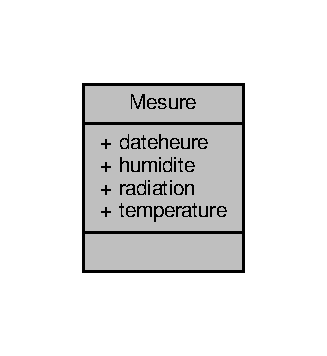
\includegraphics[width=157pt]{struct_mesure__coll__graph}
\end{center}
\end{figure}
\subsubsection*{Attributs publics}
\begin{DoxyCompactItemize}
\item 
Q\+Date\+Time \hyperlink{struct_mesure_a9958b0440aca6af40028e742123afd9e}{dateheure}
\begin{DoxyCompactList}\small\item\em Date/\+Heure. \end{DoxyCompactList}\item 
Q\+String \hyperlink{struct_mesure_ad354ba4d8a32c05600859c76a8af0282}{humidite}
\begin{DoxyCompactList}\small\item\em Donnée humidité \end{DoxyCompactList}\item 
Q\+String \hyperlink{struct_mesure_a1dae237cf09302d426ea375b9afb12f7}{radiation}
\begin{DoxyCompactList}\small\item\em Donnée radiation. \end{DoxyCompactList}\item 
Q\+String \hyperlink{struct_mesure_ad0dba8933e4b65b3781be7811f0f86ac}{temperature}
\begin{DoxyCompactList}\small\item\em Donnée temperature. \end{DoxyCompactList}\end{DoxyCompactItemize}


\subsubsection{Description détaillée}
structure permettant de définir les propriété d\textquotesingle{}une mesure prise à une heure précise 

Définition à la ligne \hyperlink{campagne_8h_source_l00021}{21} du fichier \hyperlink{campagne_8h_source}{campagne.\+h}.



\subsubsection{Documentation des données membres}
\mbox{\Hypertarget{struct_mesure_a9958b0440aca6af40028e742123afd9e}\label{struct_mesure_a9958b0440aca6af40028e742123afd9e}} 
\index{Mesure@{Mesure}!dateheure@{dateheure}}
\index{dateheure@{dateheure}!Mesure@{Mesure}}
\paragraph{\texorpdfstring{dateheure}{dateheure}}
{\footnotesize\ttfamily Q\+Date\+Time Mesure\+::dateheure}



Date/\+Heure. 



Définition à la ligne \hyperlink{campagne_8h_source_l00023}{23} du fichier \hyperlink{campagne_8h_source}{campagne.\+h}.



Référencé par \hyperlink{rov_8cpp_source_l00086}{Rov\+::decoder\+Trame\+Capteur()}.

\mbox{\Hypertarget{struct_mesure_ad354ba4d8a32c05600859c76a8af0282}\label{struct_mesure_ad354ba4d8a32c05600859c76a8af0282}} 
\index{Mesure@{Mesure}!humidite@{humidite}}
\index{humidite@{humidite}!Mesure@{Mesure}}
\paragraph{\texorpdfstring{humidite}{humidite}}
{\footnotesize\ttfamily Q\+String Mesure\+::humidite}



Donnée humidité 



Définition à la ligne \hyperlink{campagne_8h_source_l00024}{24} du fichier \hyperlink{campagne_8h_source}{campagne.\+h}.



Référencé par \hyperlink{rov_8cpp_source_l00086}{Rov\+::decoder\+Trame\+Capteur()}.

\mbox{\Hypertarget{struct_mesure_a1dae237cf09302d426ea375b9afb12f7}\label{struct_mesure_a1dae237cf09302d426ea375b9afb12f7}} 
\index{Mesure@{Mesure}!radiation@{radiation}}
\index{radiation@{radiation}!Mesure@{Mesure}}
\paragraph{\texorpdfstring{radiation}{radiation}}
{\footnotesize\ttfamily Q\+String Mesure\+::radiation}



Donnée radiation. 



Définition à la ligne \hyperlink{campagne_8h_source_l00026}{26} du fichier \hyperlink{campagne_8h_source}{campagne.\+h}.



Référencé par \hyperlink{rov_8cpp_source_l00086}{Rov\+::decoder\+Trame\+Capteur()}.

\mbox{\Hypertarget{struct_mesure_ad0dba8933e4b65b3781be7811f0f86ac}\label{struct_mesure_ad0dba8933e4b65b3781be7811f0f86ac}} 
\index{Mesure@{Mesure}!temperature@{temperature}}
\index{temperature@{temperature}!Mesure@{Mesure}}
\paragraph{\texorpdfstring{temperature}{temperature}}
{\footnotesize\ttfamily Q\+String Mesure\+::temperature}



Donnée temperature. 



Définition à la ligne \hyperlink{campagne_8h_source_l00025}{25} du fichier \hyperlink{campagne_8h_source}{campagne.\+h}.



Référencé par \hyperlink{rov_8cpp_source_l00086}{Rov\+::decoder\+Trame\+Capteur()}.



La documentation de cette structure a été générée à partir du fichier suivant \+:\begin{DoxyCompactItemize}
\item 
\hyperlink{campagne_8h}{campagne.\+h}\end{DoxyCompactItemize}

\hypertarget{struct_photo}{}\subsection{Référence de la structure Photo}
\label{struct_photo}\index{Photo@{Photo}}


structure contenant les informations d\textquotesingle{}une photo de campagne  




{\ttfamily \#include $<$ihmalbumphoto.\+h$>$}



Graphe de collaboration de Photo\+:\nopagebreak
\begin{figure}[H]
\begin{center}
\leavevmode
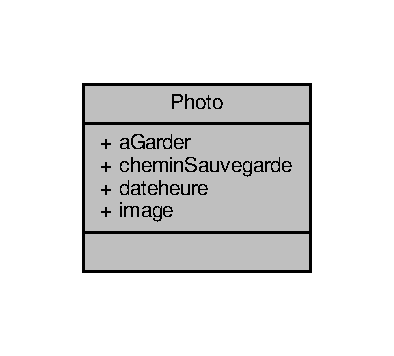
\includegraphics[width=189pt]{struct_photo__coll__graph}
\end{center}
\end{figure}
\subsubsection*{Attributs publics}
\begin{DoxyCompactItemize}
\item 
bool \hyperlink{struct_photo_afec1baefdd7d036432494bbb33b21366}{a\+Garder}
\begin{DoxyCompactList}\small\item\em Booléen afin de savoir si la photo sera archivé ou non. \end{DoxyCompactList}\item 
Q\+String \hyperlink{struct_photo_a3c28eb9ad160b65deb46a72146a1d14f}{chemin\+Sauvegarde}
\begin{DoxyCompactList}\small\item\em Chemin de sauvegarde de la photo. \end{DoxyCompactList}\item 
Q\+Time \hyperlink{struct_photo_a0ac4d5bba2d119ca73ba949d18a557bd}{dateheure}
\begin{DoxyCompactList}\small\item\em Date/\+Heure de la photo. \end{DoxyCompactList}\item 
Q\+Pixmap \hyperlink{struct_photo_aa6ecfed8082bea5af2905208308a6adb}{image}
\begin{DoxyCompactList}\small\item\em Image de la photo. \end{DoxyCompactList}\end{DoxyCompactItemize}


\subsubsection{Description détaillée}
structure contenant les informations d\textquotesingle{}une photo de campagne 

Définition à la ligne \hyperlink{ihmalbumphoto_8h_source_l00020}{20} du fichier \hyperlink{ihmalbumphoto_8h_source}{ihmalbumphoto.\+h}.



\subsubsection{Documentation des données membres}
\mbox{\Hypertarget{struct_photo_afec1baefdd7d036432494bbb33b21366}\label{struct_photo_afec1baefdd7d036432494bbb33b21366}} 
\index{Photo@{Photo}!a\+Garder@{a\+Garder}}
\index{a\+Garder@{a\+Garder}!Photo@{Photo}}
\paragraph{\texorpdfstring{a\+Garder}{aGarder}}
{\footnotesize\ttfamily bool Photo\+::a\+Garder}



Booléen afin de savoir si la photo sera archivé ou non. 



Définition à la ligne \hyperlink{ihmalbumphoto_8h_source_l00024}{24} du fichier \hyperlink{ihmalbumphoto_8h_source}{ihmalbumphoto.\+h}.



Référencé par \hyperlink{ihmrov_8cpp_source_l00179}{I\+H\+M\+Rov\+::capturer\+Image()}, et \hyperlink{ihmaccueil_8cpp_source_l00130}{I\+H\+M\+Accueil\+::charger\+Campagnes()}.

\mbox{\Hypertarget{struct_photo_a3c28eb9ad160b65deb46a72146a1d14f}\label{struct_photo_a3c28eb9ad160b65deb46a72146a1d14f}} 
\index{Photo@{Photo}!chemin\+Sauvegarde@{chemin\+Sauvegarde}}
\index{chemin\+Sauvegarde@{chemin\+Sauvegarde}!Photo@{Photo}}
\paragraph{\texorpdfstring{chemin\+Sauvegarde}{cheminSauvegarde}}
{\footnotesize\ttfamily Q\+String Photo\+::chemin\+Sauvegarde}



Chemin de sauvegarde de la photo. 



Définition à la ligne \hyperlink{ihmalbumphoto_8h_source_l00025}{25} du fichier \hyperlink{ihmalbumphoto_8h_source}{ihmalbumphoto.\+h}.



Référencé par \hyperlink{ihmaccueil_8cpp_source_l00313}{I\+H\+M\+Accueil\+::ajouter\+Photo\+B\+D\+D()}, \hyperlink{ihmrov_8cpp_source_l00179}{I\+H\+M\+Rov\+::capturer\+Image()}, et \hyperlink{ihmaccueil_8cpp_source_l00130}{I\+H\+M\+Accueil\+::charger\+Campagnes()}.

\mbox{\Hypertarget{struct_photo_a0ac4d5bba2d119ca73ba949d18a557bd}\label{struct_photo_a0ac4d5bba2d119ca73ba949d18a557bd}} 
\index{Photo@{Photo}!dateheure@{dateheure}}
\index{dateheure@{dateheure}!Photo@{Photo}}
\paragraph{\texorpdfstring{dateheure}{dateheure}}
{\footnotesize\ttfamily Q\+Time Photo\+::dateheure}



Date/\+Heure de la photo. 



Définition à la ligne \hyperlink{ihmalbumphoto_8h_source_l00023}{23} du fichier \hyperlink{ihmalbumphoto_8h_source}{ihmalbumphoto.\+h}.



Référencé par \hyperlink{ihmrov_8cpp_source_l00179}{I\+H\+M\+Rov\+::capturer\+Image()}.

\mbox{\Hypertarget{struct_photo_aa6ecfed8082bea5af2905208308a6adb}\label{struct_photo_aa6ecfed8082bea5af2905208308a6adb}} 
\index{Photo@{Photo}!image@{image}}
\index{image@{image}!Photo@{Photo}}
\paragraph{\texorpdfstring{image}{image}}
{\footnotesize\ttfamily Q\+Pixmap Photo\+::image}



Image de la photo. 



Définition à la ligne \hyperlink{ihmalbumphoto_8h_source_l00022}{22} du fichier \hyperlink{ihmalbumphoto_8h_source}{ihmalbumphoto.\+h}.



Référencé par \hyperlink{ihmrov_8cpp_source_l00179}{I\+H\+M\+Rov\+::capturer\+Image()}, et \hyperlink{ihmaccueil_8cpp_source_l00130}{I\+H\+M\+Accueil\+::charger\+Campagnes()}.



La documentation de cette structure a été générée à partir du fichier suivant \+:\begin{DoxyCompactItemize}
\item 
\hyperlink{ihmalbumphoto_8h}{ihmalbumphoto.\+h}\end{DoxyCompactItemize}

\hypertarget{class_q_dialog}{}\subsection{Référence de la classe Q\+Dialog}
\label{class_q_dialog}\index{Q\+Dialog@{Q\+Dialog}}


La classe \hyperlink{class_q_dialog}{Q\+Dialog} est la classe de base des fenêtres de dialogue.  




Graphe de collaboration de Q\+Dialog\+:\nopagebreak
\begin{figure}[H]
\begin{center}
\leavevmode
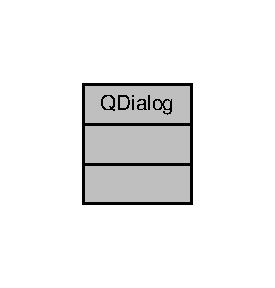
\includegraphics[width=132pt]{class_q_dialog__coll__graph}
\end{center}
\end{figure}


\subsubsection{Description détaillée}
La classe \hyperlink{class_q_dialog}{Q\+Dialog} est la classe de base des fenêtres de dialogue. 

La documentation de cette classe a été générée à partir du fichier suivant \+:\begin{DoxyCompactItemize}
\item 
\hyperlink{main_8cpp}{main.\+cpp}\end{DoxyCompactItemize}

\hypertarget{class_q_gamepad}{}\subsection{Référence de la classe Q\+Gamepad}
\label{class_q_gamepad}\index{Q\+Gamepad@{Q\+Gamepad}}


La classe \hyperlink{class_q_gamepad}{Q\+Gamepad} est utilisée pour accéder à l\textquotesingle{}état actuel du matériel de la manette de jeu connecté à un système.  




Graphe de collaboration de Q\+Gamepad\+:\nopagebreak
\begin{figure}[H]
\begin{center}
\leavevmode
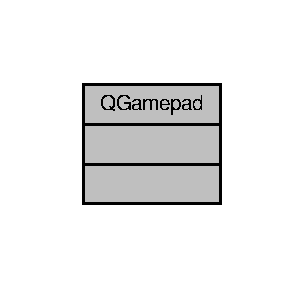
\includegraphics[width=146pt]{class_q_gamepad__coll__graph}
\end{center}
\end{figure}


\subsubsection{Description détaillée}
La classe \hyperlink{class_q_gamepad}{Q\+Gamepad} est utilisée pour accéder à l\textquotesingle{}état actuel du matériel de la manette de jeu connecté à un système. 

La documentation de cette classe a été générée à partir du fichier suivant \+:\begin{DoxyCompactItemize}
\item 
\hyperlink{main_8cpp}{main.\+cpp}\end{DoxyCompactItemize}

\hypertarget{class_q_object}{}\subsection{Référence de la classe Q\+Object}
\label{class_q_object}\index{Q\+Object@{Q\+Object}}


La classe \hyperlink{class_q_object}{Q\+Object} est la classe de base de tous les objets Qt. Elle permet à ces objets Qt de disposer entre autres du mécanisme de communication signal/slot.  




Graphe de collaboration de Q\+Object\+:\nopagebreak
\begin{figure}[H]
\begin{center}
\leavevmode
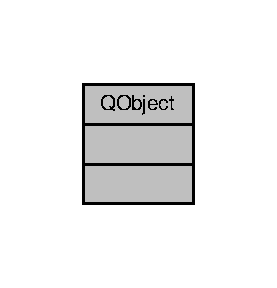
\includegraphics[width=133pt]{class_q_object__coll__graph}
\end{center}
\end{figure}


\subsubsection{Description détaillée}
La classe \hyperlink{class_q_object}{Q\+Object} est la classe de base de tous les objets Qt. Elle permet à ces objets Qt de disposer entre autres du mécanisme de communication signal/slot. 

La documentation de cette classe a été générée à partir du fichier suivant \+:\begin{DoxyCompactItemize}
\item 
\hyperlink{main_8cpp}{main.\+cpp}\end{DoxyCompactItemize}

\hypertarget{class_q_thread}{}\subsection{Référence de la classe Q\+Thread}
\label{class_q_thread}\index{Q\+Thread@{Q\+Thread}}


La classe \hyperlink{class_q_thread}{Q\+Thread} fournit un moyen indépendant de gérer les threads dans Qt.  




Graphe de collaboration de Q\+Thread\+:\nopagebreak
\begin{figure}[H]
\begin{center}
\leavevmode
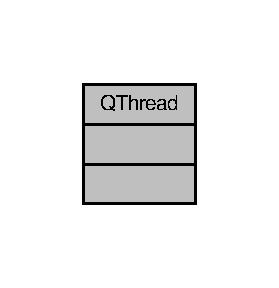
\includegraphics[width=134pt]{class_q_thread__coll__graph}
\end{center}
\end{figure}


\subsubsection{Description détaillée}
La classe \hyperlink{class_q_thread}{Q\+Thread} fournit un moyen indépendant de gérer les threads dans Qt. 

La documentation de cette classe a été générée à partir du fichier suivant \+:\begin{DoxyCompactItemize}
\item 
\hyperlink{main_8cpp}{main.\+cpp}\end{DoxyCompactItemize}

\hypertarget{class_q_widget}{}\subsection{Référence de la classe Q\+Widget}
\label{class_q_widget}\index{Q\+Widget@{Q\+Widget}}


La classe \hyperlink{class_q_widget}{Q\+Widget} est la classe de base de tous les objets graphiques d\textquotesingle{}interface utilisateur.  




Graphe de collaboration de Q\+Widget\+:\nopagebreak
\begin{figure}[H]
\begin{center}
\leavevmode
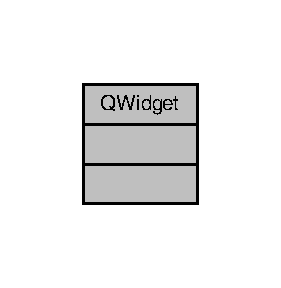
\includegraphics[width=135pt]{class_q_widget__coll__graph}
\end{center}
\end{figure}


\subsubsection{Description détaillée}
La classe \hyperlink{class_q_widget}{Q\+Widget} est la classe de base de tous les objets graphiques d\textquotesingle{}interface utilisateur. 

La documentation de cette classe a été générée à partir du fichier suivant \+:\begin{DoxyCompactItemize}
\item 
\hyperlink{main_8cpp}{main.\+cpp}\end{DoxyCompactItemize}

\hypertarget{class_rov}{}\subsection{Référence de la classe Rov}
\label{class_rov}\index{Rov@{Rov}}


Classe controlant tout les traitements en provenance et en direction de la communication avec le rov.  




{\ttfamily \#include \char`\"{}rov.\+h\char`\"{}}



Graphe de collaboration de Rov\+:
\nopagebreak
\begin{figure}[H]
\begin{center}
\leavevmode
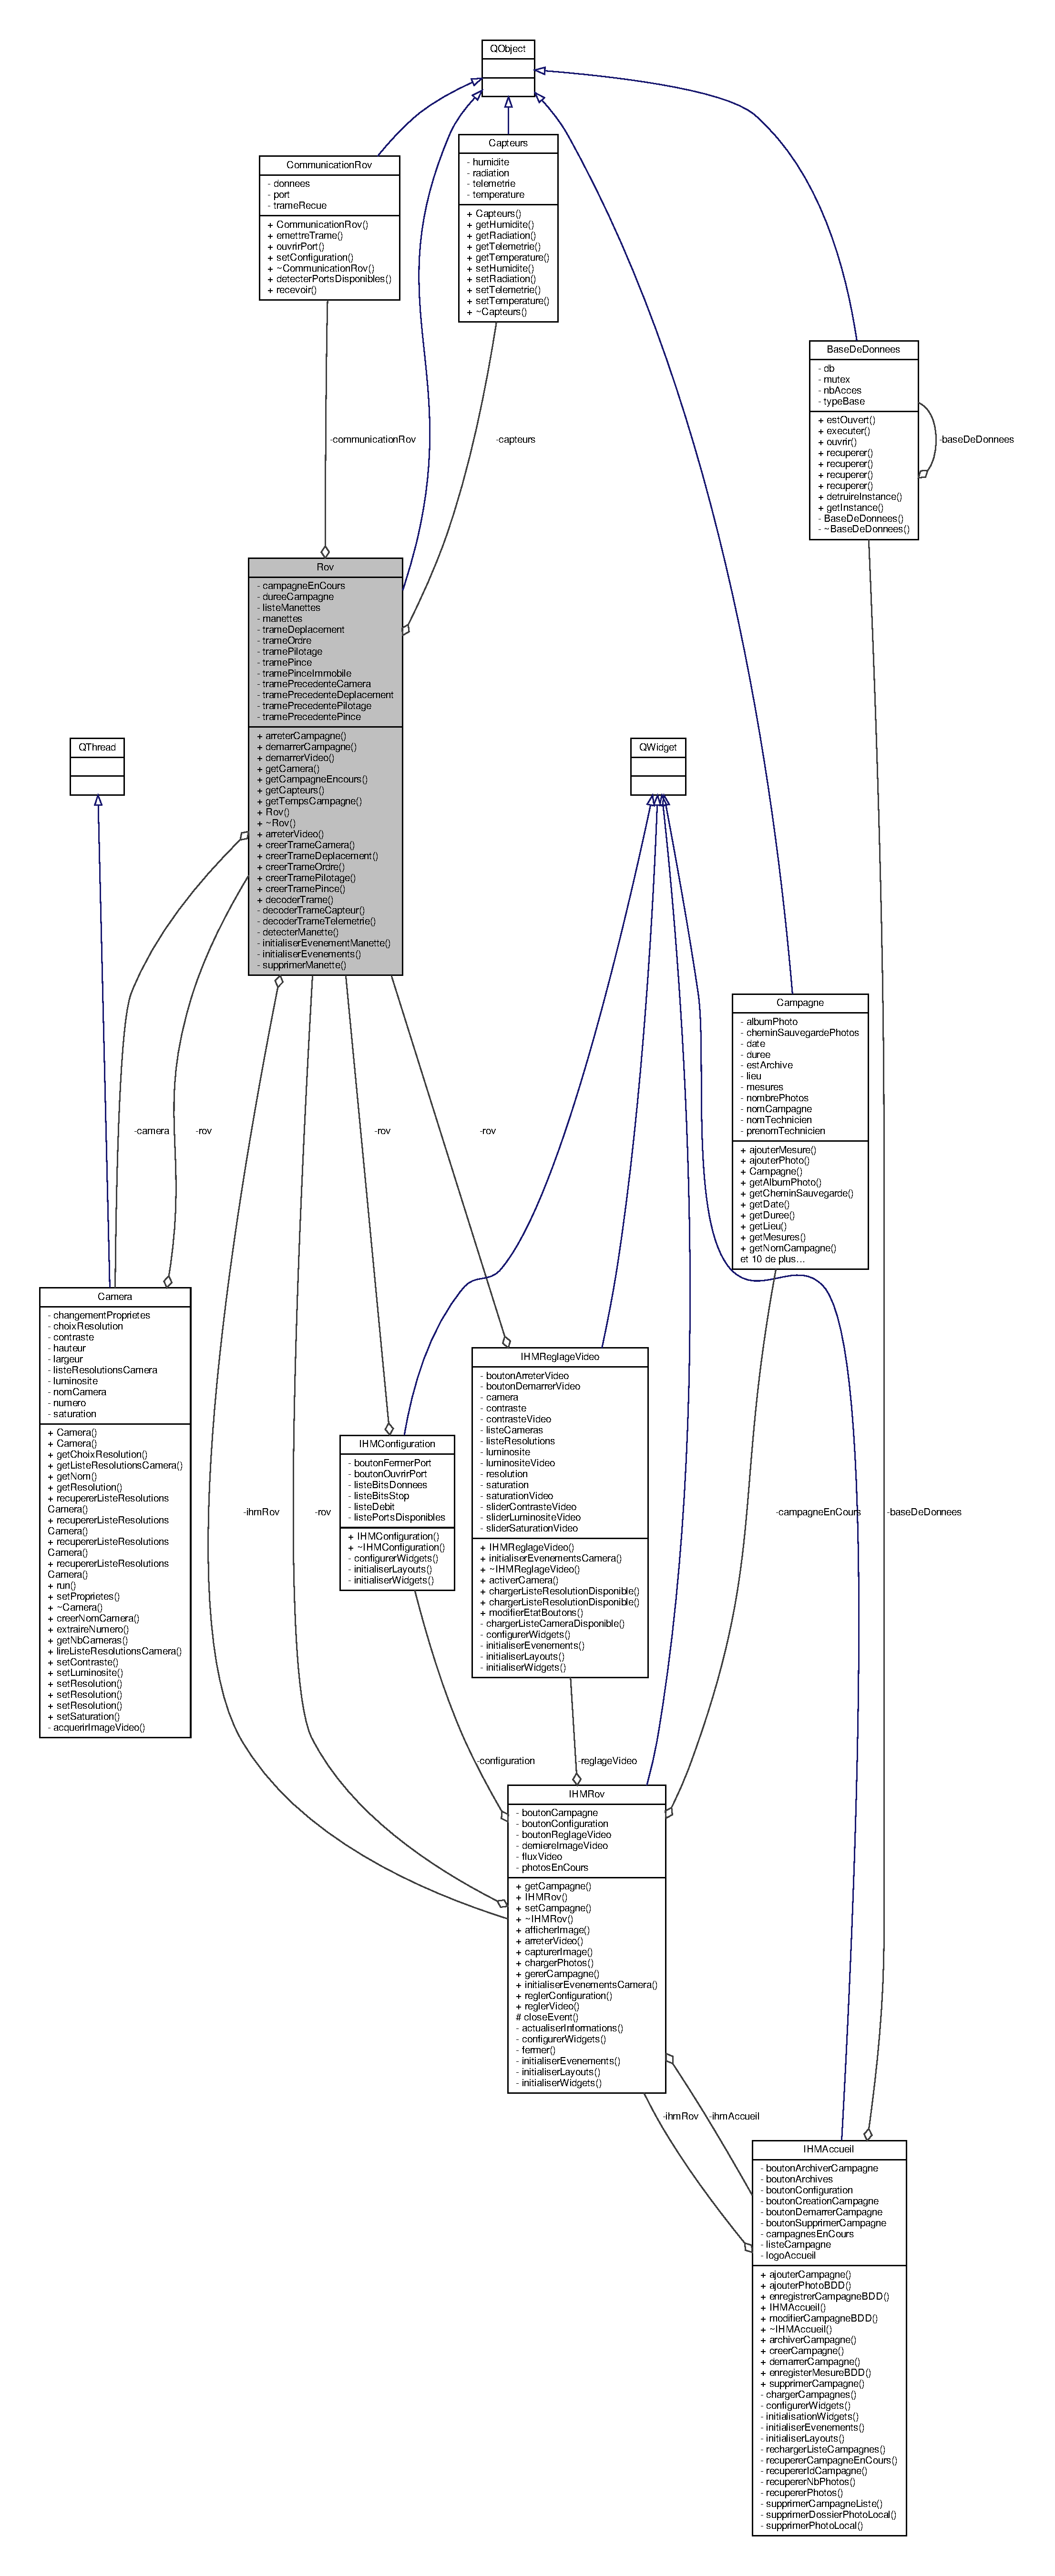
\includegraphics[height=550pt]{class_rov__coll__graph}
\end{center}
\end{figure}
\subsubsection*{Connecteurs publics}
\begin{DoxyCompactItemize}
\item 
void \hyperlink{class_rov_a241368439666a2549faff42931d82dfb}{arreter\+Video} ()
\begin{DoxyCompactList}\small\item\em Arrete le flux vidéo. \end{DoxyCompactList}\item 
void \hyperlink{class_rov_a204b1f4efe5a89f4458d84e17858e7c8}{creer\+Trame\+Camera} (Q\+String axeX, Q\+String axeY)
\begin{DoxyCompactList}\small\item\em Crée les trames de la caméra. \end{DoxyCompactList}\item 
void \hyperlink{class_rov_aa264d0723f6b491425ac2f85b933bab2}{creer\+Trame\+Deplacement} (char deplacement\+AxeX, int puissance, char deplacement\+AxeY)
\begin{DoxyCompactList}\small\item\em Crée les trames de déplacement. \end{DoxyCompactList}\item 
void \hyperlink{class_rov_a9e80eccfada890561e8af1f3426f6a2b}{creer\+Trame\+Ordre} (Q\+String ordre)
\begin{DoxyCompactList}\small\item\em Crée les trames d\textquotesingle{}ordre. \end{DoxyCompactList}\item 
void \hyperlink{class_rov_a97be62676ab0d57d5a8ac498147905ec}{creer\+Trame\+Pilotage} (Q\+String deplacement)
\begin{DoxyCompactList}\small\item\em Crée les trames de pilotage. \end{DoxyCompactList}\item 
void \hyperlink{class_rov_a66be7f6ff6e20da160d55e0cd0605965}{creer\+Trame\+Pince} (Q\+String mouvement\+Pince)
\begin{DoxyCompactList}\small\item\em Crée les trames de la pince. \end{DoxyCompactList}\item 
void \hyperlink{class_rov_ad818ff6ee1210ae44a24106b2bbbee7d}{decoder\+Trame} (Q\+String trame)
\begin{DoxyCompactList}\small\item\em Décode la trame réçue par le port série selon le protocole établie. \end{DoxyCompactList}\end{DoxyCompactItemize}
\subsubsection*{Signaux}
\begin{DoxyCompactItemize}
\item 
void \hyperlink{class_rov_ae868f3f3d691fcd6ecb97ee770541475}{donnees\+Telemetrie\+Decode} (Q\+String donnes)
\begin{DoxyCompactList}\small\item\em signal contenant les nouvelle données de télémetrie (pour l\textquotesingle{}ihm) \end{DoxyCompactList}\item 
void \hyperlink{class_rov_a180b955cc5ee7e01196299377e0c5f33}{enregistrer\+Mesures} (Q\+String temperature, Q\+String humidite, Q\+String radiation)
\begin{DoxyCompactList}\small\item\em signal contenant les nouvelles mesures recus du robot (pour les enregistrer dans la B\+DD) \end{DoxyCompactList}\end{DoxyCompactItemize}
\subsubsection*{Fonctions membres publiques}
\begin{DoxyCompactItemize}
\item 
void \hyperlink{class_rov_ad53e8d86817c81f92e3113b0394bedc5}{arreter\+Campagne} ()
\begin{DoxyCompactList}\small\item\em Arrête la campagne. \end{DoxyCompactList}\item 
bool \hyperlink{class_rov_ab20c6d0a73d6b20d4bef9e9236535a3d}{demarrer\+Campagne} ()
\begin{DoxyCompactList}\small\item\em Démarre la campagne. \end{DoxyCompactList}\item 
bool \hyperlink{class_rov_aaf1a53557b6e8f0ae2497a0af93bd6db}{demarrer\+Video} (Q\+String nom\+Camera, int choix\+Resolution=-\/1)
\begin{DoxyCompactList}\small\item\em Démarre un nouveau flux vidéo. \end{DoxyCompactList}\item 
\hyperlink{class_camera}{Camera} $\ast$ \hyperlink{class_rov_ac1eeb568d39018359b89384c2ee6ee86}{get\+Camera} ()
\begin{DoxyCompactList}\small\item\em Retourne l\textquotesingle{}objet caméra créée par le rov. \end{DoxyCompactList}\item 
bool \hyperlink{class_rov_a59d1a6d2ca83324e6efc0b74f2cff686}{get\+Campagne\+Encours} () const
\begin{DoxyCompactList}\small\item\em Retourne l\textquotesingle{}etat de la campagne. \end{DoxyCompactList}\item 
\hyperlink{class_capteurs}{Capteurs} $\ast$ \hyperlink{class_rov_a7e231245b39e7cc8026324e337b34c64}{get\+Capteurs} ()
\begin{DoxyCompactList}\small\item\em Retourne l\textquotesingle{}objet capteurs créée par le rov. \end{DoxyCompactList}\item 
Q\+String \hyperlink{class_rov_aa977585d4377a57281004fd57208635a}{get\+Temps\+Campagne} ()
\begin{DoxyCompactList}\small\item\em Retourne la durée de la campagne. \end{DoxyCompactList}\item 
\hyperlink{class_rov_a6e893548f3aadca5660540feb74f06f4}{Rov} (\hyperlink{class_i_h_m_rov}{I\+H\+M\+Rov} $\ast$\hyperlink{class_rov_a9b1c1c3b4e268a32e69b2ea4c863b817}{ihm\+Rov}, \hyperlink{class_q_object}{Q\+Object} $\ast$parent=nullptr)
\begin{DoxyCompactList}\small\item\em Constructeur de la classe \hyperlink{class_rov}{Rov}. \end{DoxyCompactList}\item 
\hyperlink{class_rov_a6e41f712195b9af74fd75b781745d1b5}{$\sim$\+Rov} ()
\begin{DoxyCompactList}\small\item\em Destructeur de la classe \hyperlink{class_rov}{Rov}. \end{DoxyCompactList}\end{DoxyCompactItemize}
\subsubsection*{Fonctions membres privées}
\begin{DoxyCompactItemize}
\item 
void \hyperlink{class_rov_ac1780c0484f427807f6207d17b564221}{decoder\+Trame\+Capteur} (Q\+String trame\+Capteur)
\begin{DoxyCompactList}\small\item\em Décode la trame capteur reçue selon le protocole. \end{DoxyCompactList}\item 
void \hyperlink{class_rov_a0d51099f9e1991ceffa0b6ed4a1c4e2e}{decoder\+Trame\+Telemetrie} (Q\+String trame\+Telemetrie)
\begin{DoxyCompactList}\small\item\em Décode la trame télémetrie reçue selon le protocole. \end{DoxyCompactList}\item 
void \hyperlink{class_rov_a53979bc347cda7cc30d18324f2146be1}{detecter\+Manette} ()
\begin{DoxyCompactList}\small\item\em detecte les mannettes \end{DoxyCompactList}\item 
void \hyperlink{class_rov_a0d1863d7d230c0153253d7d2689429b5}{initialiser\+Evenement\+Manette} (\hyperlink{class_manette}{Manette} $\ast$manette)
\begin{DoxyCompactList}\small\item\em Initialise les evenement de la manette. \end{DoxyCompactList}\item 
void \hyperlink{class_rov_a3ba4939b5d1cbd837b9c42869e6b8114}{initialiser\+Evenements} ()
\begin{DoxyCompactList}\small\item\em Initialise le(s) Evenement(s) \end{DoxyCompactList}\item 
void \hyperlink{class_rov_a31f810925200612a6bb4728236c695ed}{supprimer\+Manette} ()
\begin{DoxyCompactList}\small\item\em Supprime les manettes du conteneur des manettes. \end{DoxyCompactList}\end{DoxyCompactItemize}
\subsubsection*{Attributs privés}
\begin{DoxyCompactItemize}
\item 
\hyperlink{class_camera}{Camera} $\ast$ \hyperlink{class_rov_ad0461ecece812497ee9b4a962f168c18}{camera}
\begin{DoxyCompactList}\small\item\em Instance d\textquotesingle{}un objet camera possedant les informations nécessaire à l\textquotesingle{}affichage du flux vidéo. \end{DoxyCompactList}\item 
bool \hyperlink{class_rov_abc9d61d10d8fb5e99283d3775baf98a8}{campagne\+En\+Cours}
\begin{DoxyCompactList}\small\item\em Etat de si une campagne est en cour. \end{DoxyCompactList}\item 
\hyperlink{class_capteurs}{Capteurs} $\ast$ \hyperlink{class_rov_a1b34d63d505da660be27b75ad93754c3}{capteurs}
\begin{DoxyCompactList}\small\item\em Instance d\textquotesingle{}un objet contenant les dernières informations issues des capteurs du rov. \end{DoxyCompactList}\item 
\hyperlink{class_communication_rov}{Communication\+Rov} $\ast$ \hyperlink{class_rov_a8e7aaa17ee2134f26d57241d11ab2a99}{communication\+Rov}
\begin{DoxyCompactList}\small\item\em Instance d\textquotesingle{}un objet permettant la récupération des trames envoyé par la liaison série. \end{DoxyCompactList}\item 
Q\+Time \hyperlink{class_rov_a148a0ff28fc2dbed7b65466d77297b8a}{duree\+Campagne}
\begin{DoxyCompactList}\small\item\em Timer lancer au début de la campagne. \end{DoxyCompactList}\item 
\hyperlink{class_i_h_m_rov}{I\+H\+M\+Rov} $\ast$ \hyperlink{class_rov_a9b1c1c3b4e268a32e69b2ea4c863b817}{ihm\+Rov}
\begin{DoxyCompactList}\small\item\em Instance d\textquotesingle{}un objet ihm\+Rov permettant la connexion entre les autre classe associé aux rov et l\textquotesingle{}ihm. \end{DoxyCompactList}\item 
Q\+List$<$ int $>$ \hyperlink{class_rov_ac3bf6c7552073bd2d780e005205919a9}{liste\+Manettes}
\begin{DoxyCompactList}\small\item\em Liste des mannettes connecté \end{DoxyCompactList}\item 
Q\+Vector$<$ \hyperlink{class_manette}{Manette} $\ast$ $>$ \hyperlink{class_rov_a58ea20dc3615a732b87ac381bf1c0a83}{manettes}
\begin{DoxyCompactList}\small\item\em Conteneur des manettes. \end{DoxyCompactList}\item 
Q\+String \hyperlink{class_rov_ad30a06154c31cdb02eb28a0c7197731f}{trame\+Deplacement}
\begin{DoxyCompactList}\small\item\em Contenu trame déplacement. \end{DoxyCompactList}\item 
Q\+String \hyperlink{class_rov_aa813010d76738e268a4bbe3773663a38}{trame\+Ordre}
\begin{DoxyCompactList}\small\item\em Contenu trame ordre. \end{DoxyCompactList}\item 
Q\+String \hyperlink{class_rov_a379b288ce69a0bb9eaac8f673db8ae07}{trame\+Pilotage}
\begin{DoxyCompactList}\small\item\em Contenu trame pilotage. \end{DoxyCompactList}\item 
Q\+String \hyperlink{class_rov_a2c24d7c884d8fae07e452105037f8e2c}{trame\+Pince}
\begin{DoxyCompactList}\small\item\em Contenu trame pince. \end{DoxyCompactList}\item 
Q\+String \hyperlink{class_rov_a30595a8bd60324832b6a6eb5b542d211}{trame\+Pince\+Immobile}
\begin{DoxyCompactList}\small\item\em Contenu trame pince à zéro. \end{DoxyCompactList}\item 
Q\+String \hyperlink{class_rov_a66e64595d9bb97dfbfa6f2ed9548b216}{trame\+Precedente\+Camera}
\begin{DoxyCompactList}\small\item\em Contenu précédente trame caméra. \end{DoxyCompactList}\item 
Q\+String \hyperlink{class_rov_a6e42b166c837f5103b53bb9eae35f087}{trame\+Precedente\+Deplacement}
\begin{DoxyCompactList}\small\item\em Contenu précédente trame déplacement. \end{DoxyCompactList}\item 
Q\+String \hyperlink{class_rov_a12b08128a49ca43fc1198fdeb6a6f0cd}{trame\+Precedente\+Pilotage}
\begin{DoxyCompactList}\small\item\em Contenu précédente trame pilotage. \end{DoxyCompactList}\item 
Q\+String \hyperlink{class_rov_aa8ee68edaa542473e1e5ea6bc24432ce}{trame\+Precedente\+Pince}
\begin{DoxyCompactList}\small\item\em Contenu précédente trame pince. \end{DoxyCompactList}\end{DoxyCompactItemize}


\subsubsection{Description détaillée}
Classe controlant tout les traitements en provenance et en direction de la communication avec le rov. 

Définition à la ligne \hyperlink{rov_8h_source_l00090}{90} du fichier \hyperlink{rov_8h_source}{rov.\+h}.



\subsubsection{Documentation des constructeurs et destructeur}
\mbox{\Hypertarget{class_rov_a6e893548f3aadca5660540feb74f06f4}\label{class_rov_a6e893548f3aadca5660540feb74f06f4}} 
\index{Rov@{Rov}!Rov@{Rov}}
\index{Rov@{Rov}!Rov@{Rov}}
\paragraph{\texorpdfstring{Rov()}{Rov()}}
{\footnotesize\ttfamily Rov\+::\+Rov (\begin{DoxyParamCaption}\item[{\hyperlink{class_i_h_m_rov}{I\+H\+M\+Rov} $\ast$}]{ihm\+Rov,  }\item[{\hyperlink{class_q_object}{Q\+Object} $\ast$}]{parent = {\ttfamily nullptr} }\end{DoxyParamCaption})}



Constructeur de la classe \hyperlink{class_rov}{Rov}. 


\begin{DoxyParams}{Paramètres}
{\em ihm\+Rov} & \\
\hline
{\em parent} & \\
\hline
\end{DoxyParams}


Définition à la ligne \hyperlink{rov_8cpp_source_l00011}{11} du fichier \hyperlink{rov_8cpp_source}{rov.\+cpp}.



Références \hyperlink{rov_8h_source_l00095}{capteurs}, \hyperlink{rov_8h_source_l00097}{communication\+Rov}, \hyperlink{rov_8cpp_source_l00029}{detecter\+Manette()}, et \hyperlink{rov_8cpp_source_l00112}{initialiser\+Evenements()}.


\begin{DoxyCode}
00011                                         : \hyperlink{class_q_object}{QObject}(parent), \hyperlink{class_rov_a9b1c1c3b4e268a32e69b2ea4c863b817}{ihmRov}(ihmRov), 
      \hyperlink{class_rov_ad0461ecece812497ee9b4a962f168c18}{camera}(\textcolor{keyword}{nullptr}), \hyperlink{class_rov_ad30a06154c31cdb02eb28a0c7197731f}{trameDeplacement}(\textcolor{stringliteral}{"$DEP;0;0;0\(\backslash\)r\(\backslash\)n"}), 
      \hyperlink{class_rov_a6e42b166c837f5103b53bb9eae35f087}{tramePrecedenteDeplacement}(\textcolor{stringliteral}{"$DEP;0;0;0\(\backslash\)r\(\backslash\)n"}), 
      \hyperlink{class_rov_a379b288ce69a0bb9eaac8f673db8ae07}{tramePilotage}(\textcolor{stringliteral}{"$BRAS;0\(\backslash\)r\(\backslash\)n"}), \hyperlink{class_rov_a12b08128a49ca43fc1198fdeb6a6f0cd}{tramePrecedentePilotage}(\textcolor{stringliteral}{"$BRAS;0\(\backslash\)r\(\backslash\)n"}), 
      \hyperlink{class_rov_a2c24d7c884d8fae07e452105037f8e2c}{tramePince}(\textcolor{stringliteral}{"$PINCE;0\(\backslash\)r\(\backslash\)n"}), \hyperlink{class_rov_aa8ee68edaa542473e1e5ea6bc24432ce}{tramePrecedentePince}(\textcolor{stringliteral}{"$PINCE;0\(\backslash\)r\(\backslash\)n"}), 
      \hyperlink{class_rov_a66e64595d9bb97dfbfa6f2ed9548b216}{tramePrecedenteCamera}(\hyperlink{rov_8h_a12ba48a9aa995ebb4c7a7ace01808a2e}{TRAME\_CAMERA\_IMMOBILE}),
00012 \hyperlink{class_rov_abc9d61d10d8fb5e99283d3775baf98a8}{campagneEnCours}(\textcolor{keyword}{false})
00013 \{
00014     qDebug() << Q\_FUNC\_INFO;
00015     \hyperlink{class_rov_a8e7aaa17ee2134f26d57241d11ab2a99}{communicationRov} = \textcolor{keyword}{new} \hyperlink{class_communication_rov}{CommunicationRov}(\textcolor{keyword}{this});
00016     \hyperlink{class_rov_a1b34d63d505da660be27b75ad93754c3}{capteurs} = \textcolor{keyword}{new} \hyperlink{class_capteurs}{Capteurs}(\textcolor{keyword}{this});
00017 
00018     \hyperlink{class_rov_a3ba4939b5d1cbd837b9c42869e6b8114}{initialiserEvenements}();
00019     \hyperlink{class_rov_a53979bc347cda7cc30d18324f2146be1}{detecterManette}();
00020 \}
\end{DoxyCode}
\mbox{\Hypertarget{class_rov_a6e41f712195b9af74fd75b781745d1b5}\label{class_rov_a6e41f712195b9af74fd75b781745d1b5}} 
\index{Rov@{Rov}!````~Rov@{$\sim$\+Rov}}
\index{````~Rov@{$\sim$\+Rov}!Rov@{Rov}}
\paragraph{\texorpdfstring{$\sim$\+Rov()}{~Rov()}}
{\footnotesize\ttfamily Rov\+::$\sim$\+Rov (\begin{DoxyParamCaption}{ }\end{DoxyParamCaption})}



Destructeur de la classe \hyperlink{class_rov}{Rov}. 



Définition à la ligne \hyperlink{rov_8cpp_source_l00022}{22} du fichier \hyperlink{rov_8cpp_source}{rov.\+cpp}.



Références \hyperlink{rov_8cpp_source_l00136}{arreter\+Campagne()}, et \hyperlink{rov_8cpp_source_l00117}{supprimer\+Manette()}.


\begin{DoxyCode}
00023 \{
00024     \hyperlink{class_rov_a31f810925200612a6bb4728236c695ed}{supprimerManette}();
00025     \hyperlink{class_rov_ad53e8d86817c81f92e3113b0394bedc5}{arreterCampagne}();
00026     qDebug() << Q\_FUNC\_INFO;
00027 \}
\end{DoxyCode}


\subsubsection{Documentation des fonctions membres}
\mbox{\Hypertarget{class_rov_ad53e8d86817c81f92e3113b0394bedc5}\label{class_rov_ad53e8d86817c81f92e3113b0394bedc5}} 
\index{Rov@{Rov}!arreter\+Campagne@{arreter\+Campagne}}
\index{arreter\+Campagne@{arreter\+Campagne}!Rov@{Rov}}
\paragraph{\texorpdfstring{arreter\+Campagne()}{arreterCampagne()}}
{\footnotesize\ttfamily void Rov\+::arreter\+Campagne (\begin{DoxyParamCaption}{ }\end{DoxyParamCaption})}



Arrête la campagne. 



Définition à la ligne \hyperlink{rov_8cpp_source_l00136}{136} du fichier \hyperlink{rov_8cpp_source}{rov.\+cpp}.



Références \hyperlink{rov_8cpp_source_l00263}{arreter\+Video()}, \hyperlink{rov_8h_source_l00110}{campagne\+En\+Cours}, \hyperlink{rov_8h_source_l00109}{duree\+Campagne}, \hyperlink{ihmrov_8cpp_source_l00149}{I\+H\+M\+Rov\+::get\+Campagne()}, \hyperlink{rov_8h_source_l00094}{ihm\+Rov}, et \hyperlink{campagne_8cpp_source_l00049}{Campagne\+::set\+Duree()}.



Référencé par \hyperlink{ihmrov_8cpp_source_l00253}{I\+H\+M\+Rov\+::fermer()}, et \hyperlink{rov_8cpp_source_l00022}{$\sim$\+Rov()}.


\begin{DoxyCode}
00137 \{
00138     qDebug() << Q\_FUNC\_INFO;
00139     \hyperlink{class_rov_a9b1c1c3b4e268a32e69b2ea4c863b817}{ihmRov}->\hyperlink{class_i_h_m_rov_ab3e8686eef9233b4c1e6711cf1c4576a}{getCampagne}()->\hyperlink{class_campagne_aff9aebbc64c40ce2c1b5ae584c7a8d71}{setDuree}(\hyperlink{class_rov_a148a0ff28fc2dbed7b65466d77297b8a}{dureeCampagne}.elapsed());
00140     \hyperlink{class_rov_a241368439666a2549faff42931d82dfb}{arreterVideo}();
00141     \hyperlink{class_rov_abc9d61d10d8fb5e99283d3775baf98a8}{campagneEnCours} = \textcolor{keyword}{false};
00142 \}
\end{DoxyCode}
\mbox{\Hypertarget{class_rov_a241368439666a2549faff42931d82dfb}\label{class_rov_a241368439666a2549faff42931d82dfb}} 
\index{Rov@{Rov}!arreter\+Video@{arreter\+Video}}
\index{arreter\+Video@{arreter\+Video}!Rov@{Rov}}
\paragraph{\texorpdfstring{arreter\+Video}{arreterVideo}}
{\footnotesize\ttfamily void Rov\+::arreter\+Video (\begin{DoxyParamCaption}{ }\end{DoxyParamCaption})\hspace{0.3cm}{\ttfamily [slot]}}



Arrete le flux vidéo. 



Définition à la ligne \hyperlink{rov_8cpp_source_l00263}{263} du fichier \hyperlink{rov_8cpp_source}{rov.\+cpp}.



Références \hyperlink{ihmrov_8cpp_source_l00234}{I\+H\+M\+Rov\+::arreter\+Video()}, \hyperlink{rov_8h_source_l00096}{camera}, et \hyperlink{rov_8h_source_l00094}{ihm\+Rov}.



Référencé par \hyperlink{rov_8cpp_source_l00136}{arreter\+Campagne()}.


\begin{DoxyCode}
00264 \{
00265     \textcolor{keywordflow}{if}(\hyperlink{class_rov_ad0461ecece812497ee9b4a962f168c18}{camera} != \textcolor{keyword}{nullptr})
00266     \{
00267         qDebug() << Q\_FUNC\_INFO << \textcolor{stringliteral}{"isRunning"} << \hyperlink{class_rov_ad0461ecece812497ee9b4a962f168c18}{camera}->isRunning();
00268         \hyperlink{class_rov_a9b1c1c3b4e268a32e69b2ea4c863b817}{ihmRov}->\hyperlink{class_i_h_m_rov_a81335964f1443d11e0929017b2f21267}{arreterVideo}();
00269         disconnect(\hyperlink{class_rov_ad0461ecece812497ee9b4a962f168c18}{camera}, SIGNAL(nouvelleImage(QPixmap)), \hyperlink{class_rov_a9b1c1c3b4e268a32e69b2ea4c863b817}{ihmRov}, SLOT(afficherImage(QPixmap))
      );
00270         \hyperlink{class_rov_ad0461ecece812497ee9b4a962f168c18}{camera}->requestInterruption();
00271         \hyperlink{class_rov_ad0461ecece812497ee9b4a962f168c18}{camera}->wait();
00272         \textcolor{keyword}{delete} \hyperlink{class_rov_ad0461ecece812497ee9b4a962f168c18}{camera};
00273         \hyperlink{class_rov_ad0461ecece812497ee9b4a962f168c18}{camera} = \textcolor{keyword}{nullptr};
00274     \}
00275 \}
\end{DoxyCode}
\mbox{\Hypertarget{class_rov_a204b1f4efe5a89f4458d84e17858e7c8}\label{class_rov_a204b1f4efe5a89f4458d84e17858e7c8}} 
\index{Rov@{Rov}!creer\+Trame\+Camera@{creer\+Trame\+Camera}}
\index{creer\+Trame\+Camera@{creer\+Trame\+Camera}!Rov@{Rov}}
\paragraph{\texorpdfstring{creer\+Trame\+Camera}{creerTrameCamera}}
{\footnotesize\ttfamily void Rov\+::creer\+Trame\+Camera (\begin{DoxyParamCaption}\item[{Q\+String}]{axeX,  }\item[{Q\+String}]{axeY }\end{DoxyParamCaption})\hspace{0.3cm}{\ttfamily [slot]}}



Crée les trames de la caméra. 


\begin{DoxyParams}{Paramètres}
{\em axeX} & \\
\hline
{\em axeY} & \\
\hline
\end{DoxyParams}


Définition à la ligne \hyperlink{rov_8cpp_source_l00251}{251} du fichier \hyperlink{rov_8cpp_source}{rov.\+cpp}.



Références \hyperlink{rov_8h_source_l00097}{communication\+Rov}, \hyperlink{rov_8h_source_l00070}{D\+E\+B\+U\+T\+\_\+\+T\+R\+A\+M\+E\+\_\+\+C\+A\+M\+E\+RA}, \hyperlink{communicationrov_8cpp_source_l00060}{Communication\+Rov\+::emettre\+Trame()}, et \hyperlink{rov_8h_source_l00107}{trame\+Precedente\+Camera}.



Référencé par \hyperlink{rov_8cpp_source_l00052}{initialiser\+Evenement\+Manette()}.


\begin{DoxyCode}
00252 \{
00253     QString trameCamera = \hyperlink{rov_8h_adc800d68618fc04d8386c438c5a890ca}{DEBUT\_TRAME\_CAMERA} \textcolor{stringliteral}{";"} + axeX + \textcolor{stringliteral}{";"} + axeY + \textcolor{stringliteral}{"\(\backslash\)r\(\backslash\)n"};
00254 
00255     \textcolor{keywordflow}{if}(\hyperlink{class_rov_a66e64595d9bb97dfbfa6f2ed9548b216}{tramePrecedenteCamera} != trameCamera)
00256     \{
00257         \hyperlink{class_rov_a66e64595d9bb97dfbfa6f2ed9548b216}{tramePrecedenteCamera} = trameCamera;
00258         \hyperlink{class_rov_a8e7aaa17ee2134f26d57241d11ab2a99}{communicationRov}->\hyperlink{class_communication_rov_a4f52076db8d6e78abe1745fa1e235272}{emettreTrame}(trameCamera);
00259         qDebug() << Q\_FUNC\_INFO << \textcolor{stringliteral}{"trame camera"} << trameCamera;
00260     \}
00261 \}
\end{DoxyCode}
\mbox{\Hypertarget{class_rov_aa264d0723f6b491425ac2f85b933bab2}\label{class_rov_aa264d0723f6b491425ac2f85b933bab2}} 
\index{Rov@{Rov}!creer\+Trame\+Deplacement@{creer\+Trame\+Deplacement}}
\index{creer\+Trame\+Deplacement@{creer\+Trame\+Deplacement}!Rov@{Rov}}
\paragraph{\texorpdfstring{creer\+Trame\+Deplacement}{creerTrameDeplacement}}
{\footnotesize\ttfamily void Rov\+::creer\+Trame\+Deplacement (\begin{DoxyParamCaption}\item[{char}]{deplacement\+AxeX,  }\item[{int}]{puissance,  }\item[{char}]{deplacement\+AxeY }\end{DoxyParamCaption})\hspace{0.3cm}{\ttfamily [slot]}}



Crée les trames de déplacement. 



Définition à la ligne \hyperlink{rov_8cpp_source_l00208}{208} du fichier \hyperlink{rov_8cpp_source}{rov.\+cpp}.



Références \hyperlink{rov_8h_source_l00097}{communication\+Rov}, \hyperlink{rov_8h_source_l00034}{D\+E\+B\+U\+T\+\_\+\+T\+R\+A\+M\+E\+\_\+\+D\+E\+P\+L\+A\+C\+E\+M\+E\+NT}, \hyperlink{communicationrov_8cpp_source_l00060}{Communication\+Rov\+::emettre\+Trame()}, \hyperlink{rov_8h_source_l00100}{trame\+Deplacement}, et \hyperlink{rov_8h_source_l00101}{trame\+Precedente\+Deplacement}.



Référencé par \hyperlink{rov_8cpp_source_l00052}{initialiser\+Evenement\+Manette()}.


\begin{DoxyCode}
00209 \{
00210     \hyperlink{class_rov_ad30a06154c31cdb02eb28a0c7197731f}{trameDeplacement} = \hyperlink{rov_8h_a5bebf7c0b48103d44a372f28cf7f8981}{DEBUT\_TRAME\_DEPLACEMENT} \textcolor{stringliteral}{";"} + QString(
      deplacementAxeX) + \textcolor{stringliteral}{";"} + QString::number(puissance) + \textcolor{stringliteral}{";"} + QString(deplacementAxeY) + \textcolor{stringliteral}{"\(\backslash\)r\(\backslash\)n"};
00211     \textcolor{keywordflow}{if}(\hyperlink{class_rov_a6e42b166c837f5103b53bb9eae35f087}{tramePrecedenteDeplacement} != \hyperlink{class_rov_ad30a06154c31cdb02eb28a0c7197731f}{trameDeplacement})
00212     \{
00213         qDebug() << Q\_FUNC\_INFO << \textcolor{stringliteral}{"trameDeplacement :"} << \hyperlink{class_rov_ad30a06154c31cdb02eb28a0c7197731f}{trameDeplacement};
00214         \hyperlink{class_rov_a6e42b166c837f5103b53bb9eae35f087}{tramePrecedenteDeplacement} = \hyperlink{class_rov_ad30a06154c31cdb02eb28a0c7197731f}{trameDeplacement};
00215         \hyperlink{class_rov_a8e7aaa17ee2134f26d57241d11ab2a99}{communicationRov}->\hyperlink{class_communication_rov_a4f52076db8d6e78abe1745fa1e235272}{emettreTrame}(trameDeplacement);
00216     \}
00217 \}
\end{DoxyCode}
\mbox{\Hypertarget{class_rov_a9e80eccfada890561e8af1f3426f6a2b}\label{class_rov_a9e80eccfada890561e8af1f3426f6a2b}} 
\index{Rov@{Rov}!creer\+Trame\+Ordre@{creer\+Trame\+Ordre}}
\index{creer\+Trame\+Ordre@{creer\+Trame\+Ordre}!Rov@{Rov}}
\paragraph{\texorpdfstring{creer\+Trame\+Ordre}{creerTrameOrdre}}
{\footnotesize\ttfamily void Rov\+::creer\+Trame\+Ordre (\begin{DoxyParamCaption}\item[{Q\+String}]{ordre }\end{DoxyParamCaption})\hspace{0.3cm}{\ttfamily [slot]}}



Crée les trames d\textquotesingle{}ordre. 


\begin{DoxyParams}{Paramètres}
{\em ordre} & \\
\hline
\end{DoxyParams}


Définition à la ligne \hyperlink{rov_8cpp_source_l00230}{230} du fichier \hyperlink{rov_8cpp_source}{rov.\+cpp}.



Références \hyperlink{rov_8h_source_l00097}{communication\+Rov}, \hyperlink{rov_8h_source_l00046}{D\+E\+B\+U\+T\+\_\+\+T\+R\+A\+M\+E\+\_\+\+O\+R\+D\+RE}, \hyperlink{communicationrov_8cpp_source_l00060}{Communication\+Rov\+::emettre\+Trame()}, \hyperlink{rov_8h_source_l00058}{T\+R\+A\+M\+E\+\_\+\+P\+I\+L\+O\+T\+A\+G\+E\+\_\+\+I\+M\+M\+O\+B\+I\+LE}, \hyperlink{rov_8h_source_l00064}{T\+R\+A\+M\+E\+\_\+\+P\+I\+N\+C\+E\+\_\+\+I\+M\+M\+O\+B\+I\+LE}, \hyperlink{rov_8h_source_l00104}{trame\+Ordre}, \hyperlink{rov_8h_source_l00105}{trame\+Pince}, et \hyperlink{rov_8h_source_l00103}{trame\+Precedente\+Pilotage}.



Référencé par \hyperlink{rov_8cpp_source_l00052}{initialiser\+Evenement\+Manette()}.


\begin{DoxyCode}
00231 \{
00232     \hyperlink{class_rov_aa813010d76738e268a4bbe3773663a38}{trameOrdre} = \hyperlink{rov_8h_a8b313ffefec16809296d06146e0e75c8}{DEBUT\_TRAME\_ORDRE} \textcolor{stringliteral}{";"} + ordre + \textcolor{stringliteral}{"\(\backslash\)r\(\backslash\)n"};
00233     \textcolor{keywordflow}{if}(\hyperlink{class_rov_a12b08128a49ca43fc1198fdeb6a6f0cd}{tramePrecedentePilotage} == \hyperlink{rov_8h_ab218eea9b0b6d799e400a0d1ff835c13}{TRAME\_PILOTAGE\_IMMOBILE} && 
      \hyperlink{class_rov_a2c24d7c884d8fae07e452105037f8e2c}{tramePince} == \hyperlink{rov_8h_ab46e52d96e193353eadd9cd7f598f670}{TRAME\_PINCE\_IMMOBILE})
00234     \{
00235         qDebug() << Q\_FUNC\_INFO << \textcolor{stringliteral}{"trameOrdre :"} << \hyperlink{class_rov_aa813010d76738e268a4bbe3773663a38}{trameOrdre};
00236         \hyperlink{class_rov_a8e7aaa17ee2134f26d57241d11ab2a99}{communicationRov}->\hyperlink{class_communication_rov_a4f52076db8d6e78abe1745fa1e235272}{emettreTrame}(trameOrdre);
00237     \}
00238 \}
\end{DoxyCode}
\mbox{\Hypertarget{class_rov_a97be62676ab0d57d5a8ac498147905ec}\label{class_rov_a97be62676ab0d57d5a8ac498147905ec}} 
\index{Rov@{Rov}!creer\+Trame\+Pilotage@{creer\+Trame\+Pilotage}}
\index{creer\+Trame\+Pilotage@{creer\+Trame\+Pilotage}!Rov@{Rov}}
\paragraph{\texorpdfstring{creer\+Trame\+Pilotage}{creerTramePilotage}}
{\footnotesize\ttfamily void Rov\+::creer\+Trame\+Pilotage (\begin{DoxyParamCaption}\item[{Q\+String}]{deplacement }\end{DoxyParamCaption})\hspace{0.3cm}{\ttfamily [slot]}}



Crée les trames de pilotage. 


\begin{DoxyParams}{Paramètres}
{\em deplacement} & \\
\hline
\end{DoxyParams}


Définition à la ligne \hyperlink{rov_8cpp_source_l00219}{219} du fichier \hyperlink{rov_8cpp_source}{rov.\+cpp}.



Références \hyperlink{rov_8h_source_l00097}{communication\+Rov}, \hyperlink{rov_8h_source_l00040}{D\+E\+B\+U\+T\+\_\+\+T\+R\+A\+M\+E\+\_\+\+P\+I\+L\+O\+T\+A\+GE}, \hyperlink{communicationrov_8cpp_source_l00060}{Communication\+Rov\+::emettre\+Trame()}, \hyperlink{rov_8h_source_l00064}{T\+R\+A\+M\+E\+\_\+\+P\+I\+N\+C\+E\+\_\+\+I\+M\+M\+O\+B\+I\+LE}, \hyperlink{rov_8h_source_l00102}{trame\+Pilotage}, \hyperlink{rov_8h_source_l00105}{trame\+Pince}, et \hyperlink{rov_8h_source_l00103}{trame\+Precedente\+Pilotage}.



Référencé par \hyperlink{rov_8cpp_source_l00052}{initialiser\+Evenement\+Manette()}.


\begin{DoxyCode}
00220 \{
00221     \hyperlink{class_rov_a379b288ce69a0bb9eaac8f673db8ae07}{tramePilotage} = \hyperlink{rov_8h_a023822fa9447e76b37e5d5c78f5c64f9}{DEBUT\_TRAME\_PILOTAGE} \textcolor{stringliteral}{";"} + deplacement + \textcolor{stringliteral}{"\(\backslash\)r\(\backslash\)n"};
00222     \textcolor{keywordflow}{if}(\hyperlink{class_rov_a12b08128a49ca43fc1198fdeb6a6f0cd}{tramePrecedentePilotage} != \hyperlink{class_rov_a379b288ce69a0bb9eaac8f673db8ae07}{tramePilotage} && 
      \hyperlink{class_rov_a2c24d7c884d8fae07e452105037f8e2c}{tramePince} == \hyperlink{rov_8h_ab46e52d96e193353eadd9cd7f598f670}{TRAME\_PINCE\_IMMOBILE})
00223     \{
00224         qDebug() << Q\_FUNC\_INFO << \textcolor{stringliteral}{"tramePilotage :"} << \hyperlink{class_rov_a379b288ce69a0bb9eaac8f673db8ae07}{tramePilotage};
00225         \hyperlink{class_rov_a12b08128a49ca43fc1198fdeb6a6f0cd}{tramePrecedentePilotage} = \hyperlink{class_rov_a379b288ce69a0bb9eaac8f673db8ae07}{tramePilotage};
00226         \hyperlink{class_rov_a8e7aaa17ee2134f26d57241d11ab2a99}{communicationRov}->\hyperlink{class_communication_rov_a4f52076db8d6e78abe1745fa1e235272}{emettreTrame}(tramePilotage);
00227     \}
00228 \}
\end{DoxyCode}
\mbox{\Hypertarget{class_rov_a66be7f6ff6e20da160d55e0cd0605965}\label{class_rov_a66be7f6ff6e20da160d55e0cd0605965}} 
\index{Rov@{Rov}!creer\+Trame\+Pince@{creer\+Trame\+Pince}}
\index{creer\+Trame\+Pince@{creer\+Trame\+Pince}!Rov@{Rov}}
\paragraph{\texorpdfstring{creer\+Trame\+Pince}{creerTramePince}}
{\footnotesize\ttfamily void Rov\+::creer\+Trame\+Pince (\begin{DoxyParamCaption}\item[{Q\+String}]{mouvement\+Pince }\end{DoxyParamCaption})\hspace{0.3cm}{\ttfamily [slot]}}



Crée les trames de la pince. 


\begin{DoxyParams}{Paramètres}
{\em mouvement\+Pince} & \\
\hline
\end{DoxyParams}


Définition à la ligne \hyperlink{rov_8cpp_source_l00240}{240} du fichier \hyperlink{rov_8cpp_source}{rov.\+cpp}.



Références \hyperlink{rov_8h_source_l00097}{communication\+Rov}, \hyperlink{rov_8h_source_l00052}{D\+E\+B\+U\+T\+\_\+\+T\+R\+A\+M\+E\+\_\+\+P\+I\+N\+CE}, \hyperlink{communicationrov_8cpp_source_l00060}{Communication\+Rov\+::emettre\+Trame()}, \hyperlink{rov_8h_source_l00058}{T\+R\+A\+M\+E\+\_\+\+P\+I\+L\+O\+T\+A\+G\+E\+\_\+\+I\+M\+M\+O\+B\+I\+LE}, \hyperlink{rov_8h_source_l00105}{trame\+Pince}, \hyperlink{rov_8h_source_l00103}{trame\+Precedente\+Pilotage}, et \hyperlink{rov_8h_source_l00106}{trame\+Precedente\+Pince}.



Référencé par \hyperlink{rov_8cpp_source_l00052}{initialiser\+Evenement\+Manette()}.


\begin{DoxyCode}
00241 \{
00242     \hyperlink{class_rov_a2c24d7c884d8fae07e452105037f8e2c}{tramePince} = \hyperlink{rov_8h_ab9dc0e136712ab8227078e19a43e166a}{DEBUT\_TRAME\_PINCE} \textcolor{stringliteral}{";"} + mouvementPince + \textcolor{stringliteral}{"\(\backslash\)r\(\backslash\)n"};
00243     \textcolor{keywordflow}{if}(\hyperlink{class_rov_a12b08128a49ca43fc1198fdeb6a6f0cd}{tramePrecedentePilotage} == \hyperlink{rov_8h_ab218eea9b0b6d799e400a0d1ff835c13}{TRAME\_PILOTAGE\_IMMOBILE} && 
      \hyperlink{class_rov_aa8ee68edaa542473e1e5ea6bc24432ce}{tramePrecedentePince} != \hyperlink{class_rov_a2c24d7c884d8fae07e452105037f8e2c}{tramePince})
00244     \{
00245         qDebug() << Q\_FUNC\_INFO << \textcolor{stringliteral}{"tramePince :"} << \hyperlink{class_rov_a2c24d7c884d8fae07e452105037f8e2c}{tramePince};
00246         \hyperlink{class_rov_aa8ee68edaa542473e1e5ea6bc24432ce}{tramePrecedentePince} = \hyperlink{class_rov_a2c24d7c884d8fae07e452105037f8e2c}{tramePince};
00247         \hyperlink{class_rov_a8e7aaa17ee2134f26d57241d11ab2a99}{communicationRov}->\hyperlink{class_communication_rov_a4f52076db8d6e78abe1745fa1e235272}{emettreTrame}(tramePince);
00248     \}
00249 \}
\end{DoxyCode}
\mbox{\Hypertarget{class_rov_ad818ff6ee1210ae44a24106b2bbbee7d}\label{class_rov_ad818ff6ee1210ae44a24106b2bbbee7d}} 
\index{Rov@{Rov}!decoder\+Trame@{decoder\+Trame}}
\index{decoder\+Trame@{decoder\+Trame}!Rov@{Rov}}
\paragraph{\texorpdfstring{decoder\+Trame}{decoderTrame}}
{\footnotesize\ttfamily void Rov\+::decoder\+Trame (\begin{DoxyParamCaption}\item[{Q\+String}]{trame }\end{DoxyParamCaption})\hspace{0.3cm}{\ttfamily [slot]}}



Décode la trame réçue par le port série selon le protocole établie. 


\begin{DoxyParams}{Paramètres}
{\em trame} & \\
\hline
\end{DoxyParams}


Définition à la ligne \hyperlink{rov_8cpp_source_l00180}{180} du fichier \hyperlink{rov_8cpp_source}{rov.\+cpp}.



Références \hyperlink{rov_8h_source_l00028}{D\+E\+B\+U\+T\+\_\+\+T\+R\+A\+M\+E\+\_\+\+C\+A\+P\+T\+E\+UR}, \hyperlink{rov_8h_source_l00022}{D\+E\+B\+U\+T\+\_\+\+T\+R\+A\+M\+E\+\_\+\+T\+E\+L\+E\+M\+E\+T\+R\+IE}, \hyperlink{rov_8cpp_source_l00086}{decoder\+Trame\+Capteur()}, et \hyperlink{rov_8cpp_source_l00081}{decoder\+Trame\+Telemetrie()}.



Référencé par \hyperlink{rov_8cpp_source_l00112}{initialiser\+Evenements()}.


\begin{DoxyCode}
00181 \{
00182     QString trameTelemetrie, trameCapteur;
00183 
00184     QStringList trames = trame.split(\textcolor{stringliteral}{"\(\backslash\)r\(\backslash\)n"});
00185     qDebug() << Q\_FUNC\_INFO << \textcolor{stringliteral}{"trame"} << trames.size();
00186     \textcolor{keywordflow}{for}(\textcolor{keywordtype}{int} i = 0; i < trames.size(); i++)
00187     \{
00188         \textcolor{keywordflow}{if}(!trames[i].isEmpty())
00189         \{
00190             \textcolor{keywordflow}{if}(trames[i].startsWith(\hyperlink{rov_8h_aa4d7955cdbd3d56086855ed938b980d1}{DEBUT\_TRAME\_TELEMETRIE}))
00191             \{
00192                 trameTelemetrie = trames[i];
00193                 \hyperlink{class_rov_a0d51099f9e1991ceffa0b6ed4a1c4e2e}{decoderTrameTelemetrie}(trameTelemetrie);
00194             \}
00195             \textcolor{keywordflow}{else} \textcolor{keywordflow}{if}(trames[i].startsWith(\hyperlink{rov_8h_a224f8acbc025db0e90045ce113761b0f}{DEBUT\_TRAME\_CAPTEUR}))
00196             \{
00197                 trameCapteur = trames[i];
00198                 \hyperlink{class_rov_ac1780c0484f427807f6207d17b564221}{decoderTrameCapteur}(trameCapteur);
00199             \}
00200         \}
00201         \textcolor{keywordflow}{else}
00202         \{
00203             qDebug() << Q\_FUNC\_INFO << \textcolor{stringliteral}{"Trame inconnue !"};
00204         \}
00205     \}
00206 \}
\end{DoxyCode}
\mbox{\Hypertarget{class_rov_ac1780c0484f427807f6207d17b564221}\label{class_rov_ac1780c0484f427807f6207d17b564221}} 
\index{Rov@{Rov}!decoder\+Trame\+Capteur@{decoder\+Trame\+Capteur}}
\index{decoder\+Trame\+Capteur@{decoder\+Trame\+Capteur}!Rov@{Rov}}
\paragraph{\texorpdfstring{decoder\+Trame\+Capteur()}{decoderTrameCapteur()}}
{\footnotesize\ttfamily void Rov\+::decoder\+Trame\+Capteur (\begin{DoxyParamCaption}\item[{Q\+String}]{trame\+Capteur }\end{DoxyParamCaption})\hspace{0.3cm}{\ttfamily [private]}}



Décode la trame capteur reçue selon le protocole. 


\begin{DoxyParams}{Paramètres}
{\em trame\+Capteur} & \\
\hline
\end{DoxyParams}


Définition à la ligne \hyperlink{rov_8cpp_source_l00086}{86} du fichier \hyperlink{rov_8cpp_source}{rov.\+cpp}.



Références \hyperlink{campagne_8cpp_source_l00090}{Campagne\+::ajouter\+Mesure()}, \hyperlink{rov_8h_source_l00095}{capteurs}, \hyperlink{campagne_8h_source_l00023}{Mesure\+::dateheure}, \hyperlink{class_rov_a180b955cc5ee7e01196299377e0c5f33}{enregistrer\+Mesures()}, \hyperlink{ihmrov_8cpp_source_l00149}{I\+H\+M\+Rov\+::get\+Campagne()}, \hyperlink{campagne_8h_source_l00024}{Mesure\+::humidite}, \hyperlink{rov_8h_source_l00094}{ihm\+Rov}, \hyperlink{campagne_8h_source_l00026}{Mesure\+::radiation}, \hyperlink{capteurs_8cpp_source_l00029}{Capteurs\+::set\+Humidite()}, \hyperlink{capteurs_8cpp_source_l00034}{Capteurs\+::set\+Radiation()}, \hyperlink{capteurs_8cpp_source_l00024}{Capteurs\+::set\+Temperature()}, et \hyperlink{campagne_8h_source_l00025}{Mesure\+::temperature}.



Référencé par \hyperlink{rov_8cpp_source_l00180}{decoder\+Trame()}.


\begin{DoxyCode}
00087 \{
00088     QString temperature, humidite, radiation;
00089 
00090     temperature = trameCapteur.section(\textcolor{stringliteral}{";"},1,1);
00091     humidite = trameCapteur.section(\textcolor{stringliteral}{";"},2,2);
00092     radiation = trameCapteur.section(\textcolor{stringliteral}{";"},3,3);
00093 
00094     \hyperlink{class_rov_a1b34d63d505da660be27b75ad93754c3}{capteurs}->\hyperlink{class_capteurs_a8d6a0bceb4d236edf7b51335d9be8ecd}{setTemperature}(temperature);
00095     \hyperlink{class_rov_a1b34d63d505da660be27b75ad93754c3}{capteurs}->\hyperlink{class_capteurs_aafb06e1746006cdb72e92dc7a0519a2e}{setHumidite}(humidite);
00096     \hyperlink{class_rov_a1b34d63d505da660be27b75ad93754c3}{capteurs}->\hyperlink{class_capteurs_a8692d145188df3129d88fef77efbb7b0}{setRadiation}(radiation);
00097 
00098     \hyperlink{struct_mesure}{Mesure} mesure;
00099     mesure.\hyperlink{struct_mesure_a9958b0440aca6af40028e742123afd9e}{dateheure} = QDateTime::currentDateTime();
00100     mesure.\hyperlink{struct_mesure_ad0dba8933e4b65b3781be7811f0f86ac}{temperature} = temperature;
00101     mesure.\hyperlink{struct_mesure_ad354ba4d8a32c05600859c76a8af0282}{humidite} = humidite;
00102     mesure.\hyperlink{struct_mesure_a1dae237cf09302d426ea375b9afb12f7}{radiation} = radiation;
00103 
00104     QDateTime date;
00105 
00106     \hyperlink{class_rov_a9b1c1c3b4e268a32e69b2ea4c863b817}{ihmRov}->\hyperlink{class_i_h_m_rov_ab3e8686eef9233b4c1e6711cf1c4576a}{getCampagne}()->\hyperlink{class_campagne_ab301ceaacbe1186682c2b6f3282619d0}{ajouterMesure}(mesure);
00107 
00108     emit \hyperlink{class_rov_a180b955cc5ee7e01196299377e0c5f33}{enregistrerMesures}(temperature, humidite, radiation);
00109 
00110 \}
\end{DoxyCode}
\mbox{\Hypertarget{class_rov_a0d51099f9e1991ceffa0b6ed4a1c4e2e}\label{class_rov_a0d51099f9e1991ceffa0b6ed4a1c4e2e}} 
\index{Rov@{Rov}!decoder\+Trame\+Telemetrie@{decoder\+Trame\+Telemetrie}}
\index{decoder\+Trame\+Telemetrie@{decoder\+Trame\+Telemetrie}!Rov@{Rov}}
\paragraph{\texorpdfstring{decoder\+Trame\+Telemetrie()}{decoderTrameTelemetrie()}}
{\footnotesize\ttfamily void Rov\+::decoder\+Trame\+Telemetrie (\begin{DoxyParamCaption}\item[{Q\+String}]{trame\+Telemetrie }\end{DoxyParamCaption})\hspace{0.3cm}{\ttfamily [private]}}



Décode la trame télémetrie reçue selon le protocole. 


\begin{DoxyParams}{Paramètres}
{\em trame\+Telemetrie} & \\
\hline
\end{DoxyParams}


Définition à la ligne \hyperlink{rov_8cpp_source_l00081}{81} du fichier \hyperlink{rov_8cpp_source}{rov.\+cpp}.



Références \hyperlink{rov_8h_source_l00095}{capteurs}, et \hyperlink{capteurs_8cpp_source_l00019}{Capteurs\+::set\+Telemetrie()}.



Référencé par \hyperlink{rov_8cpp_source_l00180}{decoder\+Trame()}.


\begin{DoxyCode}
00082 \{
00083     \hyperlink{class_rov_a1b34d63d505da660be27b75ad93754c3}{capteurs}->\hyperlink{class_capteurs_a399af986afb9d707138bc57a51e1f34f}{setTelemetrie}(trameTelemetrie.section(\textcolor{stringliteral}{";"},1,1));
00084 \}
\end{DoxyCode}
\mbox{\Hypertarget{class_rov_ab20c6d0a73d6b20d4bef9e9236535a3d}\label{class_rov_ab20c6d0a73d6b20d4bef9e9236535a3d}} 
\index{Rov@{Rov}!demarrer\+Campagne@{demarrer\+Campagne}}
\index{demarrer\+Campagne@{demarrer\+Campagne}!Rov@{Rov}}
\paragraph{\texorpdfstring{demarrer\+Campagne()}{demarrerCampagne()}}
{\footnotesize\ttfamily bool Rov\+::demarrer\+Campagne (\begin{DoxyParamCaption}{ }\end{DoxyParamCaption})}



Démarre la campagne. 



Définition à la ligne \hyperlink{rov_8cpp_source_l00123}{123} du fichier \hyperlink{rov_8cpp_source}{rov.\+cpp}.



Références \hyperlink{camera_8h_source_l00029}{C\+A\+M\+E\+R\+A\+\_\+\+D\+E\+F\+A\+UT}, \hyperlink{rov_8h_source_l00110}{campagne\+En\+Cours}, \hyperlink{camera_8cpp_source_l00293}{Camera\+::creer\+Nom\+Camera()}, \hyperlink{rov_8cpp_source_l00161}{demarrer\+Video()}, \hyperlink{rov_8h_source_l00109}{duree\+Campagne}, et \hyperlink{camera_8cpp_source_l00270}{Camera\+::get\+Nb\+Cameras()}.



Référencé par \hyperlink{ihmrov_8cpp_source_l00202}{I\+H\+M\+Rov\+::gerer\+Campagne()}.


\begin{DoxyCode}
00124 \{
00125     qDebug() << Q\_FUNC\_INFO;
00126     \textcolor{keywordflow}{if}(\hyperlink{class_camera_a116b3869ff0647c851715605a1938a3c}{Camera::getNbCameras}() > 0)
00127     \{
00128         \hyperlink{class_rov_a148a0ff28fc2dbed7b65466d77297b8a}{dureeCampagne}.start();
00129         QString nom = \hyperlink{class_camera_a506d459df95042a03894afd5b781c2aa}{Camera::creerNomCamera}(\hyperlink{camera_8h_a87f76384d33bc9bba579afd1d5f3221a}{CAMERA\_DEFAUT});
00130         \textcolor{keywordflow}{if}(\hyperlink{class_rov_aaf1a53557b6e8f0ae2497a0af93bd6db}{demarrerVideo}(nom))
00131             \hyperlink{class_rov_abc9d61d10d8fb5e99283d3775baf98a8}{campagneEnCours} = \textcolor{keyword}{true};
00132     \}
00133     \textcolor{keywordflow}{return} \hyperlink{class_rov_abc9d61d10d8fb5e99283d3775baf98a8}{campagneEnCours};
00134 \}
\end{DoxyCode}
\mbox{\Hypertarget{class_rov_aaf1a53557b6e8f0ae2497a0af93bd6db}\label{class_rov_aaf1a53557b6e8f0ae2497a0af93bd6db}} 
\index{Rov@{Rov}!demarrer\+Video@{demarrer\+Video}}
\index{demarrer\+Video@{demarrer\+Video}!Rov@{Rov}}
\paragraph{\texorpdfstring{demarrer\+Video()}{demarrerVideo()}}
{\footnotesize\ttfamily bool Rov\+::demarrer\+Video (\begin{DoxyParamCaption}\item[{Q\+String}]{nom\+Camera,  }\item[{int}]{choix\+Resolution = {\ttfamily -\/1} }\end{DoxyParamCaption})}



Démarre un nouveau flux vidéo. 


\begin{DoxyParams}{Paramètres}
{\em nom\+Camera} & \\
\hline
{\em choix\+Resolution} & \\
\hline
\end{DoxyParams}


Définition à la ligne \hyperlink{rov_8cpp_source_l00161}{161} du fichier \hyperlink{rov_8cpp_source}{rov.\+cpp}.



Références \hyperlink{rov_8h_source_l00096}{camera}, \hyperlink{rov_8h_source_l00094}{ihm\+Rov}, et \hyperlink{ihmrov_8cpp_source_l00229}{I\+H\+M\+Rov\+::initialiser\+Evenements\+Camera()}.



Référencé par \hyperlink{ihmreglagevideo_8cpp_source_l00203}{I\+H\+M\+Reglage\+Video\+::activer\+Camera()}, et \hyperlink{rov_8cpp_source_l00123}{demarrer\+Campagne()}.


\begin{DoxyCode}
00162 \{
00163     qDebug() << Q\_FUNC\_INFO << \textcolor{stringliteral}{"nomCamera"} << nomCamera << \textcolor{stringliteral}{"choixResolution"} << choixResolution;
00164     \textcolor{keywordflow}{if}(\hyperlink{class_rov_ad0461ecece812497ee9b4a962f168c18}{camera} == \textcolor{keyword}{nullptr})
00165     \{
00166         \hyperlink{class_rov_ad0461ecece812497ee9b4a962f168c18}{camera} = \textcolor{keyword}{new} \hyperlink{class_camera}{Camera}(\textcolor{keyword}{this}, nomCamera, choixResolution);
00167         connect(\hyperlink{class_rov_ad0461ecece812497ee9b4a962f168c18}{camera}, SIGNAL(nouvelleImage(QPixmap)), \hyperlink{class_rov_a9b1c1c3b4e268a32e69b2ea4c863b817}{ihmRov}, SLOT(afficherImage(QPixmap)));
00168         \hyperlink{class_rov_a9b1c1c3b4e268a32e69b2ea4c863b817}{ihmRov}->\hyperlink{class_i_h_m_rov_a955daa231d959666fa7ed01346b2b6ef}{initialiserEvenementsCamera}();
00169         \hyperlink{class_rov_ad0461ecece812497ee9b4a962f168c18}{camera}->start();
00170         \textcolor{keywordflow}{return} \textcolor{keyword}{true};
00171     \}
00172     \textcolor{keywordflow}{return} \textcolor{keyword}{false};
00173 \}
\end{DoxyCode}
\mbox{\Hypertarget{class_rov_a53979bc347cda7cc30d18324f2146be1}\label{class_rov_a53979bc347cda7cc30d18324f2146be1}} 
\index{Rov@{Rov}!detecter\+Manette@{detecter\+Manette}}
\index{detecter\+Manette@{detecter\+Manette}!Rov@{Rov}}
\paragraph{\texorpdfstring{detecter\+Manette()}{detecterManette()}}
{\footnotesize\ttfamily void Rov\+::detecter\+Manette (\begin{DoxyParamCaption}{ }\end{DoxyParamCaption})\hspace{0.3cm}{\ttfamily [private]}}



detecte les mannettes 



Définition à la ligne \hyperlink{rov_8cpp_source_l00029}{29} du fichier \hyperlink{rov_8cpp_source}{rov.\+cpp}.



Références \hyperlink{rov_8cpp_source_l00052}{initialiser\+Evenement\+Manette()}, \hyperlink{rov_8h_source_l00098}{liste\+Manettes}, et \hyperlink{rov_8h_source_l00099}{manettes}.



Référencé par \hyperlink{rov_8cpp_source_l00011}{Rov()}.


\begin{DoxyCode}
00030 \{
00031     \hyperlink{class_rov_ac3bf6c7552073bd2d780e005205919a9}{listeManettes} = QGamepadManager::instance()->connectedGamepads();
00032 
00033     \textcolor{keywordflow}{if} (\hyperlink{class_rov_ac3bf6c7552073bd2d780e005205919a9}{listeManettes}.isEmpty())
00034     \{
00035         qDebug() << Q\_FUNC\_INFO << \textcolor{stringliteral}{"Aucune manette détectée !"};
00036 
00037     \}
00038     \textcolor{keywordflow}{else}
00039     \{
00040         qDebug() << Q\_FUNC\_INFO << \textcolor{stringliteral}{"Nombre de manettes"} << \hyperlink{class_rov_ac3bf6c7552073bd2d780e005205919a9}{listeManettes}.size();
00041     \}
00042 
00043     \textcolor{keywordflow}{for} (\textcolor{keyword}{auto} m : \hyperlink{class_rov_ac3bf6c7552073bd2d780e005205919a9}{listeManettes})
00044     \{
00045         qDebug() << Q\_FUNC\_INFO << \textcolor{stringliteral}{"-> Manette"} << m;
00046         \hyperlink{class_manette}{Manette} *manette = \textcolor{keyword}{new} \hyperlink{class_manette}{Manette}(m);
00047         \hyperlink{class_rov_a58ea20dc3615a732b87ac381bf1c0a83}{manettes}.push\_back(manette);
00048         \hyperlink{class_rov_a0d1863d7d230c0153253d7d2689429b5}{initialiserEvenementManette}(manette);
00049     \}
00050 \}
\end{DoxyCode}
\mbox{\Hypertarget{class_rov_ae868f3f3d691fcd6ecb97ee770541475}\label{class_rov_ae868f3f3d691fcd6ecb97ee770541475}} 
\index{Rov@{Rov}!donnees\+Telemetrie\+Decode@{donnees\+Telemetrie\+Decode}}
\index{donnees\+Telemetrie\+Decode@{donnees\+Telemetrie\+Decode}!Rov@{Rov}}
\paragraph{\texorpdfstring{donnees\+Telemetrie\+Decode}{donneesTelemetrieDecode}}
{\footnotesize\ttfamily void Rov\+::donnees\+Telemetrie\+Decode (\begin{DoxyParamCaption}\item[{Q\+String}]{donnes }\end{DoxyParamCaption})\hspace{0.3cm}{\ttfamily [signal]}}



signal contenant les nouvelle données de télémetrie (pour l\textquotesingle{}ihm) 


\begin{DoxyParams}{Paramètres}
{\em donnes} & \\
\hline
\end{DoxyParams}
\mbox{\Hypertarget{class_rov_a180b955cc5ee7e01196299377e0c5f33}\label{class_rov_a180b955cc5ee7e01196299377e0c5f33}} 
\index{Rov@{Rov}!enregistrer\+Mesures@{enregistrer\+Mesures}}
\index{enregistrer\+Mesures@{enregistrer\+Mesures}!Rov@{Rov}}
\paragraph{\texorpdfstring{enregistrer\+Mesures}{enregistrerMesures}}
{\footnotesize\ttfamily void Rov\+::enregistrer\+Mesures (\begin{DoxyParamCaption}\item[{Q\+String}]{temperature,  }\item[{Q\+String}]{humidite,  }\item[{Q\+String}]{radiation }\end{DoxyParamCaption})\hspace{0.3cm}{\ttfamily [signal]}}



signal contenant les nouvelles mesures recus du robot (pour les enregistrer dans la B\+DD) 


\begin{DoxyParams}{Paramètres}
{\em temperature} & \\
\hline
{\em humidite} & \\
\hline
{\em radiation} & \\
\hline
\end{DoxyParams}


Référencé par \hyperlink{rov_8cpp_source_l00086}{decoder\+Trame\+Capteur()}.

\mbox{\Hypertarget{class_rov_ac1eeb568d39018359b89384c2ee6ee86}\label{class_rov_ac1eeb568d39018359b89384c2ee6ee86}} 
\index{Rov@{Rov}!get\+Camera@{get\+Camera}}
\index{get\+Camera@{get\+Camera}!Rov@{Rov}}
\paragraph{\texorpdfstring{get\+Camera()}{getCamera()}}
{\footnotesize\ttfamily \hyperlink{class_camera}{Camera} $\ast$ Rov\+::get\+Camera (\begin{DoxyParamCaption}{ }\end{DoxyParamCaption})}



Retourne l\textquotesingle{}objet caméra créée par le rov. 

\begin{DoxyReturn}{Renvoie}
L\textquotesingle{}objet caméra créée par le rov 
\end{DoxyReturn}


Définition à la ligne \hyperlink{rov_8cpp_source_l00144}{144} du fichier \hyperlink{rov_8cpp_source}{rov.\+cpp}.



Références \hyperlink{rov_8h_source_l00096}{camera}.



Référencé par \hyperlink{ihmreglagevideo_8cpp_source_l00132}{I\+H\+M\+Reglage\+Video\+::charger\+Liste\+Camera\+Disponible()}, \hyperlink{ihmreglagevideo_8cpp_source_l00179}{I\+H\+M\+Reglage\+Video\+::charger\+Liste\+Resolution\+Disponible()}, \hyperlink{ihmreglagevideo_8cpp_source_l00117}{I\+H\+M\+Reglage\+Video\+::initialiser\+Evenements\+Camera()}, et \hyperlink{ihmreglagevideo_8cpp_source_l00212}{I\+H\+M\+Reglage\+Video\+::modifier\+Etat\+Boutons()}.


\begin{DoxyCode}
00145 \{
00146     \textcolor{keywordflow}{return} \hyperlink{class_rov_ad0461ecece812497ee9b4a962f168c18}{camera};
00147 \}
\end{DoxyCode}
\mbox{\Hypertarget{class_rov_a59d1a6d2ca83324e6efc0b74f2cff686}\label{class_rov_a59d1a6d2ca83324e6efc0b74f2cff686}} 
\index{Rov@{Rov}!get\+Campagne\+Encours@{get\+Campagne\+Encours}}
\index{get\+Campagne\+Encours@{get\+Campagne\+Encours}!Rov@{Rov}}
\paragraph{\texorpdfstring{get\+Campagne\+Encours()}{getCampagneEncours()}}
{\footnotesize\ttfamily bool Rov\+::get\+Campagne\+Encours (\begin{DoxyParamCaption}{ }\end{DoxyParamCaption}) const}



Retourne l\textquotesingle{}etat de la campagne. 

\begin{DoxyReturn}{Renvoie}
l\textquotesingle{}etat de campagne\+En\+Cours (indiquant si la campagne est en cours ou pas) 
\end{DoxyReturn}


Définition à la ligne \hyperlink{rov_8cpp_source_l00175}{175} du fichier \hyperlink{rov_8cpp_source}{rov.\+cpp}.



Références \hyperlink{rov_8h_source_l00110}{campagne\+En\+Cours}.



Référencé par \hyperlink{ihmrov_8cpp_source_l00239}{I\+H\+M\+Rov\+::close\+Event()}.


\begin{DoxyCode}
00176 \{
00177     \textcolor{keywordflow}{return} \hyperlink{class_rov_abc9d61d10d8fb5e99283d3775baf98a8}{campagneEnCours};
00178 \}
\end{DoxyCode}
\mbox{\Hypertarget{class_rov_a7e231245b39e7cc8026324e337b34c64}\label{class_rov_a7e231245b39e7cc8026324e337b34c64}} 
\index{Rov@{Rov}!get\+Capteurs@{get\+Capteurs}}
\index{get\+Capteurs@{get\+Capteurs}!Rov@{Rov}}
\paragraph{\texorpdfstring{get\+Capteurs()}{getCapteurs()}}
{\footnotesize\ttfamily \hyperlink{class_capteurs}{Capteurs} $\ast$ Rov\+::get\+Capteurs (\begin{DoxyParamCaption}{ }\end{DoxyParamCaption})}



Retourne l\textquotesingle{}objet capteurs créée par le rov. 

\begin{DoxyReturn}{Renvoie}
L\textquotesingle{}objet capteurs créée par le rov 
\end{DoxyReturn}


Définition à la ligne \hyperlink{rov_8cpp_source_l00149}{149} du fichier \hyperlink{rov_8cpp_source}{rov.\+cpp}.



Références \hyperlink{rov_8h_source_l00095}{capteurs}.



Référencé par \hyperlink{ihmrov_8cpp_source_l00110}{I\+H\+M\+Rov\+::actualiser\+Informations()}.


\begin{DoxyCode}
00150 \{
00151     \textcolor{keywordflow}{return} \hyperlink{class_rov_a1b34d63d505da660be27b75ad93754c3}{capteurs};
00152 \}
\end{DoxyCode}
\mbox{\Hypertarget{class_rov_aa977585d4377a57281004fd57208635a}\label{class_rov_aa977585d4377a57281004fd57208635a}} 
\index{Rov@{Rov}!get\+Temps\+Campagne@{get\+Temps\+Campagne}}
\index{get\+Temps\+Campagne@{get\+Temps\+Campagne}!Rov@{Rov}}
\paragraph{\texorpdfstring{get\+Temps\+Campagne()}{getTempsCampagne()}}
{\footnotesize\ttfamily Q\+String Rov\+::get\+Temps\+Campagne (\begin{DoxyParamCaption}{ }\end{DoxyParamCaption})}



Retourne la durée de la campagne. 

\begin{DoxyReturn}{Renvoie}
La durée de la campagne 
\end{DoxyReturn}


Définition à la ligne \hyperlink{rov_8cpp_source_l00154}{154} du fichier \hyperlink{rov_8cpp_source}{rov.\+cpp}.



Références \hyperlink{rov_8h_source_l00109}{duree\+Campagne}, \hyperlink{ihmrov_8cpp_source_l00149}{I\+H\+M\+Rov\+::get\+Campagne()}, \hyperlink{campagne_8cpp_source_l00044}{Campagne\+::get\+Duree()}, et \hyperlink{rov_8h_source_l00094}{ihm\+Rov}.



Référencé par \hyperlink{ihmrov_8cpp_source_l00110}{I\+H\+M\+Rov\+::actualiser\+Informations()}.


\begin{DoxyCode}
00155 \{
00156     QTime duree(0,0);
00157     QTime dureeMission = duree.addMSecs(\hyperlink{class_rov_a148a0ff28fc2dbed7b65466d77297b8a}{dureeCampagne}.elapsed() + 
      \hyperlink{class_rov_a9b1c1c3b4e268a32e69b2ea4c863b817}{ihmRov}->\hyperlink{class_i_h_m_rov_ab3e8686eef9233b4c1e6711cf1c4576a}{getCampagne}()->\hyperlink{class_campagne_abe02a9050f4a5ea9521dd40b855c350b}{getDuree}());
00158     \textcolor{keywordflow}{return} dureeMission.toString(\textcolor{stringliteral}{"hh:mm:ss"});
00159 \}
\end{DoxyCode}
\mbox{\Hypertarget{class_rov_a0d1863d7d230c0153253d7d2689429b5}\label{class_rov_a0d1863d7d230c0153253d7d2689429b5}} 
\index{Rov@{Rov}!initialiser\+Evenement\+Manette@{initialiser\+Evenement\+Manette}}
\index{initialiser\+Evenement\+Manette@{initialiser\+Evenement\+Manette}!Rov@{Rov}}
\paragraph{\texorpdfstring{initialiser\+Evenement\+Manette()}{initialiserEvenementManette()}}
{\footnotesize\ttfamily void Rov\+::initialiser\+Evenement\+Manette (\begin{DoxyParamCaption}\item[{\hyperlink{class_manette}{Manette} $\ast$}]{manette }\end{DoxyParamCaption})\hspace{0.3cm}{\ttfamily [private]}}



Initialise les evenement de la manette. 


\begin{DoxyParams}{Paramètres}
{\em manette} & \\
\hline
\end{DoxyParams}


Définition à la ligne \hyperlink{rov_8cpp_source_l00052}{52} du fichier \hyperlink{rov_8cpp_source}{rov.\+cpp}.



Références \hyperlink{rov_8cpp_source_l00251}{creer\+Trame\+Camera()}, \hyperlink{rov_8cpp_source_l00208}{creer\+Trame\+Deplacement()}, \hyperlink{rov_8cpp_source_l00230}{creer\+Trame\+Ordre()}, \hyperlink{rov_8cpp_source_l00219}{creer\+Trame\+Pilotage()}, \hyperlink{rov_8cpp_source_l00240}{creer\+Trame\+Pince()}, et \hyperlink{rov_8h_source_l00094}{ihm\+Rov}.



Référencé par \hyperlink{rov_8cpp_source_l00029}{detecter\+Manette()}.


\begin{DoxyCode}
00053 \{
00054     connect(manette, SIGNAL(creationTrameDeplacement(\textcolor{keywordtype}{char}, \textcolor{keywordtype}{int}, \textcolor{keywordtype}{char})), \textcolor{keyword}{this}, SLOT(
      \hyperlink{class_rov_aa264d0723f6b491425ac2f85b933bab2}{creerTrameDeplacement}(\textcolor{keywordtype}{char}, \textcolor{keywordtype}{int}, \textcolor{keywordtype}{char})));
00055     connect(manette, SIGNAL(creationTramePilotage(QString)), \textcolor{keyword}{this}, SLOT(
      \hyperlink{class_rov_a97be62676ab0d57d5a8ac498147905ec}{creerTramePilotage}(QString)));
00056     connect(manette, SIGNAL(creationTrameOrdre(QString)), \textcolor{keyword}{this}, SLOT(
      \hyperlink{class_rov_a9e80eccfada890561e8af1f3426f6a2b}{creerTrameOrdre}(QString)));
00057     connect(manette, SIGNAL(creationTramePince(QString)), \textcolor{keyword}{this}, SLOT(
      \hyperlink{class_rov_a66be7f6ff6e20da160d55e0cd0605965}{creerTramePince}(QString)));
00058     connect(manette, SIGNAL(nouvelleTrameCamera(QString,QString)), \textcolor{keyword}{this}, SLOT(
      \hyperlink{class_rov_a204b1f4efe5a89f4458d84e17858e7c8}{creerTrameCamera}(QString,QString)));
00059 
00060     connect(manette, SIGNAL(axisLeftXChanged(\textcolor{keywordtype}{double})), manette, SLOT(changerAxeXJoystickGauche(\textcolor{keywordtype}{double})));
00061     connect(manette, SIGNAL(axisLeftYChanged(\textcolor{keywordtype}{double})), manette, SLOT(changerAxeYJoystickGauche(\textcolor{keywordtype}{double})));
00062     connect(manette, SIGNAL(axisRightXChanged(\textcolor{keywordtype}{double})), manette, SLOT(changerAxeXJoystickDroit(\textcolor{keywordtype}{double})));
00063     connect(manette, SIGNAL(axisRightYChanged(\textcolor{keywordtype}{double})), manette, SLOT(changerAxeYJoystickDroit(\textcolor{keywordtype}{double})));
00064     connect(manette, SIGNAL(buttonL1Changed(\textcolor{keywordtype}{bool})), manette, SLOT(changerBoutonHautGauche(\textcolor{keywordtype}{bool})));
00065     connect(manette, SIGNAL(buttonR1Changed(\textcolor{keywordtype}{bool})), manette, SLOT(changerBoutonHautDroit(\textcolor{keywordtype}{bool})));
00066     connect(manette, SIGNAL(buttonL2Changed(\textcolor{keywordtype}{double})), manette, SLOT(changerGachetteBasGauche(\textcolor{keywordtype}{double})));
00067     connect(manette, SIGNAL(buttonR2Changed(\textcolor{keywordtype}{double})), manette, SLOT(changerGachetteBasDroit(\textcolor{keywordtype}{double})));
00068     connect(manette, SIGNAL(buttonUpChanged(\textcolor{keywordtype}{bool})), manette, SLOT(changerFlecheEnAvant(\textcolor{keywordtype}{bool})));
00069     connect(manette, SIGNAL(buttonDownChanged(\textcolor{keywordtype}{bool})), manette, SLOT(changerFlecheEnArriere(\textcolor{keywordtype}{bool})));
00070     connect(manette, SIGNAL(buttonLeftChanged(\textcolor{keywordtype}{bool})), manette, SLOT(changerFlecheAGauche(\textcolor{keywordtype}{bool})));
00071     connect(manette, SIGNAL(buttonRightChanged(\textcolor{keywordtype}{bool})), manette, SLOT(changerFlecheADroite(\textcolor{keywordtype}{bool})));
00072     connect(manette, SIGNAL(buttonAChanged(\textcolor{keywordtype}{bool})), manette, SLOT(changerBoutonA(\textcolor{keywordtype}{bool})));
00073     connect(manette, SIGNAL(buttonBChanged(\textcolor{keywordtype}{bool})), manette, SLOT(changerBoutonB(\textcolor{keywordtype}{bool})));
00074     connect(manette, SIGNAL(buttonXChanged(\textcolor{keywordtype}{bool})), manette, SLOT(changerBoutonX(\textcolor{keywordtype}{bool})));
00075     connect(manette, SIGNAL(buttonYChanged(\textcolor{keywordtype}{bool})), manette, SLOT(changerBoutonY(\textcolor{keywordtype}{bool})));
00076     connect(manette, SIGNAL(buttonSelectChanged(\textcolor{keywordtype}{bool})), manette, SLOT(changerBoutonSelect(\textcolor{keywordtype}{bool})));
00077     connect(manette, SIGNAL(buttonGuideChanged(\textcolor{keywordtype}{bool})), manette, SLOT(fermerApplication(\textcolor{keywordtype}{bool})));
00078     connect(manette, SIGNAL(buttonR3Changed(\textcolor{keywordtype}{bool})), \hyperlink{class_rov_a9b1c1c3b4e268a32e69b2ea4c863b817}{ihmRov}, SLOT(capturerImage(\textcolor{keywordtype}{bool})));
00079 \}
\end{DoxyCode}
\mbox{\Hypertarget{class_rov_a3ba4939b5d1cbd837b9c42869e6b8114}\label{class_rov_a3ba4939b5d1cbd837b9c42869e6b8114}} 
\index{Rov@{Rov}!initialiser\+Evenements@{initialiser\+Evenements}}
\index{initialiser\+Evenements@{initialiser\+Evenements}!Rov@{Rov}}
\paragraph{\texorpdfstring{initialiser\+Evenements()}{initialiserEvenements()}}
{\footnotesize\ttfamily void Rov\+::initialiser\+Evenements (\begin{DoxyParamCaption}{ }\end{DoxyParamCaption})\hspace{0.3cm}{\ttfamily [private]}}



Initialise le(s) Evenement(s) 



Définition à la ligne \hyperlink{rov_8cpp_source_l00112}{112} du fichier \hyperlink{rov_8cpp_source}{rov.\+cpp}.



Références \hyperlink{rov_8h_source_l00097}{communication\+Rov}, et \hyperlink{rov_8cpp_source_l00180}{decoder\+Trame()}.



Référencé par \hyperlink{rov_8cpp_source_l00011}{Rov()}.


\begin{DoxyCode}
00113 \{
00114     connect(\hyperlink{class_rov_a8e7aaa17ee2134f26d57241d11ab2a99}{communicationRov}, SIGNAL(nouvelleTrame(QString)), \textcolor{keyword}{this}, SLOT(
      \hyperlink{class_rov_ad818ff6ee1210ae44a24106b2bbbee7d}{decoderTrame}(QString)));
00115 \}
\end{DoxyCode}
\mbox{\Hypertarget{class_rov_a31f810925200612a6bb4728236c695ed}\label{class_rov_a31f810925200612a6bb4728236c695ed}} 
\index{Rov@{Rov}!supprimer\+Manette@{supprimer\+Manette}}
\index{supprimer\+Manette@{supprimer\+Manette}!Rov@{Rov}}
\paragraph{\texorpdfstring{supprimer\+Manette()}{supprimerManette()}}
{\footnotesize\ttfamily void Rov\+::supprimer\+Manette (\begin{DoxyParamCaption}{ }\end{DoxyParamCaption})\hspace{0.3cm}{\ttfamily [private]}}



Supprime les manettes du conteneur des manettes. 



Définition à la ligne \hyperlink{rov_8cpp_source_l00117}{117} du fichier \hyperlink{rov_8cpp_source}{rov.\+cpp}.



Références \hyperlink{rov_8h_source_l00099}{manettes}.



Référencé par \hyperlink{rov_8cpp_source_l00022}{$\sim$\+Rov()}.


\begin{DoxyCode}
00118 \{
00119     \textcolor{keywordflow}{for}(\textcolor{keywordtype}{int} i=0;i<\hyperlink{class_rov_a58ea20dc3615a732b87ac381bf1c0a83}{manettes}.size();i++)
00120         \textcolor{keyword}{delete} \hyperlink{class_rov_a58ea20dc3615a732b87ac381bf1c0a83}{manettes}[i];
00121 \}
\end{DoxyCode}


\subsubsection{Documentation des données membres}
\mbox{\Hypertarget{class_rov_ad0461ecece812497ee9b4a962f168c18}\label{class_rov_ad0461ecece812497ee9b4a962f168c18}} 
\index{Rov@{Rov}!camera@{camera}}
\index{camera@{camera}!Rov@{Rov}}
\paragraph{\texorpdfstring{camera}{camera}}
{\footnotesize\ttfamily \hyperlink{class_camera}{Camera}$\ast$ Rov\+::camera\hspace{0.3cm}{\ttfamily [private]}}



Instance d\textquotesingle{}un objet camera possedant les informations nécessaire à l\textquotesingle{}affichage du flux vidéo. 



Définition à la ligne \hyperlink{rov_8h_source_l00096}{96} du fichier \hyperlink{rov_8h_source}{rov.\+h}.



Référencé par \hyperlink{rov_8cpp_source_l00263}{arreter\+Video()}, \hyperlink{rov_8cpp_source_l00161}{demarrer\+Video()}, et \hyperlink{rov_8cpp_source_l00144}{get\+Camera()}.

\mbox{\Hypertarget{class_rov_abc9d61d10d8fb5e99283d3775baf98a8}\label{class_rov_abc9d61d10d8fb5e99283d3775baf98a8}} 
\index{Rov@{Rov}!campagne\+En\+Cours@{campagne\+En\+Cours}}
\index{campagne\+En\+Cours@{campagne\+En\+Cours}!Rov@{Rov}}
\paragraph{\texorpdfstring{campagne\+En\+Cours}{campagneEnCours}}
{\footnotesize\ttfamily bool Rov\+::campagne\+En\+Cours\hspace{0.3cm}{\ttfamily [private]}}



Etat de si une campagne est en cour. 



Définition à la ligne \hyperlink{rov_8h_source_l00110}{110} du fichier \hyperlink{rov_8h_source}{rov.\+h}.



Référencé par \hyperlink{rov_8cpp_source_l00136}{arreter\+Campagne()}, \hyperlink{rov_8cpp_source_l00123}{demarrer\+Campagne()}, et \hyperlink{rov_8cpp_source_l00175}{get\+Campagne\+Encours()}.

\mbox{\Hypertarget{class_rov_a1b34d63d505da660be27b75ad93754c3}\label{class_rov_a1b34d63d505da660be27b75ad93754c3}} 
\index{Rov@{Rov}!capteurs@{capteurs}}
\index{capteurs@{capteurs}!Rov@{Rov}}
\paragraph{\texorpdfstring{capteurs}{capteurs}}
{\footnotesize\ttfamily \hyperlink{class_capteurs}{Capteurs}$\ast$ Rov\+::capteurs\hspace{0.3cm}{\ttfamily [private]}}



Instance d\textquotesingle{}un objet contenant les dernières informations issues des capteurs du rov. 



Définition à la ligne \hyperlink{rov_8h_source_l00095}{95} du fichier \hyperlink{rov_8h_source}{rov.\+h}.



Référencé par \hyperlink{rov_8cpp_source_l00086}{decoder\+Trame\+Capteur()}, \hyperlink{rov_8cpp_source_l00081}{decoder\+Trame\+Telemetrie()}, \hyperlink{rov_8cpp_source_l00149}{get\+Capteurs()}, et \hyperlink{rov_8cpp_source_l00011}{Rov()}.

\mbox{\Hypertarget{class_rov_a8e7aaa17ee2134f26d57241d11ab2a99}\label{class_rov_a8e7aaa17ee2134f26d57241d11ab2a99}} 
\index{Rov@{Rov}!communication\+Rov@{communication\+Rov}}
\index{communication\+Rov@{communication\+Rov}!Rov@{Rov}}
\paragraph{\texorpdfstring{communication\+Rov}{communicationRov}}
{\footnotesize\ttfamily \hyperlink{class_communication_rov}{Communication\+Rov}$\ast$ Rov\+::communication\+Rov\hspace{0.3cm}{\ttfamily [private]}}



Instance d\textquotesingle{}un objet permettant la récupération des trames envoyé par la liaison série. 



Définition à la ligne \hyperlink{rov_8h_source_l00097}{97} du fichier \hyperlink{rov_8h_source}{rov.\+h}.



Référencé par \hyperlink{rov_8cpp_source_l00251}{creer\+Trame\+Camera()}, \hyperlink{rov_8cpp_source_l00208}{creer\+Trame\+Deplacement()}, \hyperlink{rov_8cpp_source_l00230}{creer\+Trame\+Ordre()}, \hyperlink{rov_8cpp_source_l00219}{creer\+Trame\+Pilotage()}, \hyperlink{rov_8cpp_source_l00240}{creer\+Trame\+Pince()}, \hyperlink{rov_8cpp_source_l00112}{initialiser\+Evenements()}, et \hyperlink{rov_8cpp_source_l00011}{Rov()}.

\mbox{\Hypertarget{class_rov_a148a0ff28fc2dbed7b65466d77297b8a}\label{class_rov_a148a0ff28fc2dbed7b65466d77297b8a}} 
\index{Rov@{Rov}!duree\+Campagne@{duree\+Campagne}}
\index{duree\+Campagne@{duree\+Campagne}!Rov@{Rov}}
\paragraph{\texorpdfstring{duree\+Campagne}{dureeCampagne}}
{\footnotesize\ttfamily Q\+Time Rov\+::duree\+Campagne\hspace{0.3cm}{\ttfamily [private]}}



Timer lancer au début de la campagne. 



Définition à la ligne \hyperlink{rov_8h_source_l00109}{109} du fichier \hyperlink{rov_8h_source}{rov.\+h}.



Référencé par \hyperlink{rov_8cpp_source_l00136}{arreter\+Campagne()}, \hyperlink{rov_8cpp_source_l00123}{demarrer\+Campagne()}, et \hyperlink{rov_8cpp_source_l00154}{get\+Temps\+Campagne()}.

\mbox{\Hypertarget{class_rov_a9b1c1c3b4e268a32e69b2ea4c863b817}\label{class_rov_a9b1c1c3b4e268a32e69b2ea4c863b817}} 
\index{Rov@{Rov}!ihm\+Rov@{ihm\+Rov}}
\index{ihm\+Rov@{ihm\+Rov}!Rov@{Rov}}
\paragraph{\texorpdfstring{ihm\+Rov}{ihmRov}}
{\footnotesize\ttfamily \hyperlink{class_i_h_m_rov}{I\+H\+M\+Rov}$\ast$ Rov\+::ihm\+Rov\hspace{0.3cm}{\ttfamily [private]}}



Instance d\textquotesingle{}un objet ihm\+Rov permettant la connexion entre les autre classe associé aux rov et l\textquotesingle{}ihm. 



Définition à la ligne \hyperlink{rov_8h_source_l00094}{94} du fichier \hyperlink{rov_8h_source}{rov.\+h}.



Référencé par \hyperlink{rov_8cpp_source_l00136}{arreter\+Campagne()}, \hyperlink{rov_8cpp_source_l00263}{arreter\+Video()}, \hyperlink{rov_8cpp_source_l00086}{decoder\+Trame\+Capteur()}, \hyperlink{rov_8cpp_source_l00161}{demarrer\+Video()}, \hyperlink{rov_8cpp_source_l00154}{get\+Temps\+Campagne()}, et \hyperlink{rov_8cpp_source_l00052}{initialiser\+Evenement\+Manette()}.

\mbox{\Hypertarget{class_rov_ac3bf6c7552073bd2d780e005205919a9}\label{class_rov_ac3bf6c7552073bd2d780e005205919a9}} 
\index{Rov@{Rov}!liste\+Manettes@{liste\+Manettes}}
\index{liste\+Manettes@{liste\+Manettes}!Rov@{Rov}}
\paragraph{\texorpdfstring{liste\+Manettes}{listeManettes}}
{\footnotesize\ttfamily Q\+List$<$int$>$ Rov\+::liste\+Manettes\hspace{0.3cm}{\ttfamily [private]}}



Liste des mannettes connecté 



Définition à la ligne \hyperlink{rov_8h_source_l00098}{98} du fichier \hyperlink{rov_8h_source}{rov.\+h}.



Référencé par \hyperlink{rov_8cpp_source_l00029}{detecter\+Manette()}.

\mbox{\Hypertarget{class_rov_a58ea20dc3615a732b87ac381bf1c0a83}\label{class_rov_a58ea20dc3615a732b87ac381bf1c0a83}} 
\index{Rov@{Rov}!manettes@{manettes}}
\index{manettes@{manettes}!Rov@{Rov}}
\paragraph{\texorpdfstring{manettes}{manettes}}
{\footnotesize\ttfamily Q\+Vector$<$\hyperlink{class_manette}{Manette}$\ast$$>$ Rov\+::manettes\hspace{0.3cm}{\ttfamily [private]}}



Conteneur des manettes. 



Définition à la ligne \hyperlink{rov_8h_source_l00099}{99} du fichier \hyperlink{rov_8h_source}{rov.\+h}.



Référencé par \hyperlink{rov_8cpp_source_l00029}{detecter\+Manette()}, et \hyperlink{rov_8cpp_source_l00117}{supprimer\+Manette()}.

\mbox{\Hypertarget{class_rov_ad30a06154c31cdb02eb28a0c7197731f}\label{class_rov_ad30a06154c31cdb02eb28a0c7197731f}} 
\index{Rov@{Rov}!trame\+Deplacement@{trame\+Deplacement}}
\index{trame\+Deplacement@{trame\+Deplacement}!Rov@{Rov}}
\paragraph{\texorpdfstring{trame\+Deplacement}{trameDeplacement}}
{\footnotesize\ttfamily Q\+String Rov\+::trame\+Deplacement\hspace{0.3cm}{\ttfamily [private]}}



Contenu trame déplacement. 



Définition à la ligne \hyperlink{rov_8h_source_l00100}{100} du fichier \hyperlink{rov_8h_source}{rov.\+h}.



Référencé par \hyperlink{rov_8cpp_source_l00208}{creer\+Trame\+Deplacement()}.

\mbox{\Hypertarget{class_rov_aa813010d76738e268a4bbe3773663a38}\label{class_rov_aa813010d76738e268a4bbe3773663a38}} 
\index{Rov@{Rov}!trame\+Ordre@{trame\+Ordre}}
\index{trame\+Ordre@{trame\+Ordre}!Rov@{Rov}}
\paragraph{\texorpdfstring{trame\+Ordre}{trameOrdre}}
{\footnotesize\ttfamily Q\+String Rov\+::trame\+Ordre\hspace{0.3cm}{\ttfamily [private]}}



Contenu trame ordre. 



Définition à la ligne \hyperlink{rov_8h_source_l00104}{104} du fichier \hyperlink{rov_8h_source}{rov.\+h}.



Référencé par \hyperlink{rov_8cpp_source_l00230}{creer\+Trame\+Ordre()}.

\mbox{\Hypertarget{class_rov_a379b288ce69a0bb9eaac8f673db8ae07}\label{class_rov_a379b288ce69a0bb9eaac8f673db8ae07}} 
\index{Rov@{Rov}!trame\+Pilotage@{trame\+Pilotage}}
\index{trame\+Pilotage@{trame\+Pilotage}!Rov@{Rov}}
\paragraph{\texorpdfstring{trame\+Pilotage}{tramePilotage}}
{\footnotesize\ttfamily Q\+String Rov\+::trame\+Pilotage\hspace{0.3cm}{\ttfamily [private]}}



Contenu trame pilotage. 



Définition à la ligne \hyperlink{rov_8h_source_l00102}{102} du fichier \hyperlink{rov_8h_source}{rov.\+h}.



Référencé par \hyperlink{rov_8cpp_source_l00219}{creer\+Trame\+Pilotage()}.

\mbox{\Hypertarget{class_rov_a2c24d7c884d8fae07e452105037f8e2c}\label{class_rov_a2c24d7c884d8fae07e452105037f8e2c}} 
\index{Rov@{Rov}!trame\+Pince@{trame\+Pince}}
\index{trame\+Pince@{trame\+Pince}!Rov@{Rov}}
\paragraph{\texorpdfstring{trame\+Pince}{tramePince}}
{\footnotesize\ttfamily Q\+String Rov\+::trame\+Pince\hspace{0.3cm}{\ttfamily [private]}}



Contenu trame pince. 



Définition à la ligne \hyperlink{rov_8h_source_l00105}{105} du fichier \hyperlink{rov_8h_source}{rov.\+h}.



Référencé par \hyperlink{rov_8cpp_source_l00230}{creer\+Trame\+Ordre()}, \hyperlink{rov_8cpp_source_l00219}{creer\+Trame\+Pilotage()}, et \hyperlink{rov_8cpp_source_l00240}{creer\+Trame\+Pince()}.

\mbox{\Hypertarget{class_rov_a30595a8bd60324832b6a6eb5b542d211}\label{class_rov_a30595a8bd60324832b6a6eb5b542d211}} 
\index{Rov@{Rov}!trame\+Pince\+Immobile@{trame\+Pince\+Immobile}}
\index{trame\+Pince\+Immobile@{trame\+Pince\+Immobile}!Rov@{Rov}}
\paragraph{\texorpdfstring{trame\+Pince\+Immobile}{tramePinceImmobile}}
{\footnotesize\ttfamily Q\+String Rov\+::trame\+Pince\+Immobile\hspace{0.3cm}{\ttfamily [private]}}



Contenu trame pince à zéro. 



Définition à la ligne \hyperlink{rov_8h_source_l00108}{108} du fichier \hyperlink{rov_8h_source}{rov.\+h}.

\mbox{\Hypertarget{class_rov_a66e64595d9bb97dfbfa6f2ed9548b216}\label{class_rov_a66e64595d9bb97dfbfa6f2ed9548b216}} 
\index{Rov@{Rov}!trame\+Precedente\+Camera@{trame\+Precedente\+Camera}}
\index{trame\+Precedente\+Camera@{trame\+Precedente\+Camera}!Rov@{Rov}}
\paragraph{\texorpdfstring{trame\+Precedente\+Camera}{tramePrecedenteCamera}}
{\footnotesize\ttfamily Q\+String Rov\+::trame\+Precedente\+Camera\hspace{0.3cm}{\ttfamily [private]}}



Contenu précédente trame caméra. 



Définition à la ligne \hyperlink{rov_8h_source_l00107}{107} du fichier \hyperlink{rov_8h_source}{rov.\+h}.



Référencé par \hyperlink{rov_8cpp_source_l00251}{creer\+Trame\+Camera()}.

\mbox{\Hypertarget{class_rov_a6e42b166c837f5103b53bb9eae35f087}\label{class_rov_a6e42b166c837f5103b53bb9eae35f087}} 
\index{Rov@{Rov}!trame\+Precedente\+Deplacement@{trame\+Precedente\+Deplacement}}
\index{trame\+Precedente\+Deplacement@{trame\+Precedente\+Deplacement}!Rov@{Rov}}
\paragraph{\texorpdfstring{trame\+Precedente\+Deplacement}{tramePrecedenteDeplacement}}
{\footnotesize\ttfamily Q\+String Rov\+::trame\+Precedente\+Deplacement\hspace{0.3cm}{\ttfamily [private]}}



Contenu précédente trame déplacement. 



Définition à la ligne \hyperlink{rov_8h_source_l00101}{101} du fichier \hyperlink{rov_8h_source}{rov.\+h}.



Référencé par \hyperlink{rov_8cpp_source_l00208}{creer\+Trame\+Deplacement()}.

\mbox{\Hypertarget{class_rov_a12b08128a49ca43fc1198fdeb6a6f0cd}\label{class_rov_a12b08128a49ca43fc1198fdeb6a6f0cd}} 
\index{Rov@{Rov}!trame\+Precedente\+Pilotage@{trame\+Precedente\+Pilotage}}
\index{trame\+Precedente\+Pilotage@{trame\+Precedente\+Pilotage}!Rov@{Rov}}
\paragraph{\texorpdfstring{trame\+Precedente\+Pilotage}{tramePrecedentePilotage}}
{\footnotesize\ttfamily Q\+String Rov\+::trame\+Precedente\+Pilotage\hspace{0.3cm}{\ttfamily [private]}}



Contenu précédente trame pilotage. 



Définition à la ligne \hyperlink{rov_8h_source_l00103}{103} du fichier \hyperlink{rov_8h_source}{rov.\+h}.



Référencé par \hyperlink{rov_8cpp_source_l00230}{creer\+Trame\+Ordre()}, \hyperlink{rov_8cpp_source_l00219}{creer\+Trame\+Pilotage()}, et \hyperlink{rov_8cpp_source_l00240}{creer\+Trame\+Pince()}.

\mbox{\Hypertarget{class_rov_aa8ee68edaa542473e1e5ea6bc24432ce}\label{class_rov_aa8ee68edaa542473e1e5ea6bc24432ce}} 
\index{Rov@{Rov}!trame\+Precedente\+Pince@{trame\+Precedente\+Pince}}
\index{trame\+Precedente\+Pince@{trame\+Precedente\+Pince}!Rov@{Rov}}
\paragraph{\texorpdfstring{trame\+Precedente\+Pince}{tramePrecedentePince}}
{\footnotesize\ttfamily Q\+String Rov\+::trame\+Precedente\+Pince\hspace{0.3cm}{\ttfamily [private]}}



Contenu précédente trame pince. 



Définition à la ligne \hyperlink{rov_8h_source_l00106}{106} du fichier \hyperlink{rov_8h_source}{rov.\+h}.



Référencé par \hyperlink{rov_8cpp_source_l00240}{creer\+Trame\+Pince()}.



La documentation de cette classe a été générée à partir des fichiers suivants \+:\begin{DoxyCompactItemize}
\item 
\hyperlink{rov_8h}{rov.\+h}\item 
\hyperlink{rov_8cpp}{rov.\+cpp}\end{DoxyCompactItemize}

\section{Documentation des fichiers}
\hypertarget{basededonnees_8cpp}{}\subsection{Référence du fichier basededonnees.\+cpp}
\label{basededonnees_8cpp}\index{basededonnees.\+cpp@{basededonnees.\+cpp}}


Fichier qui contient la définition de la classe \hyperlink{class_base_de_donnees}{Base\+De\+Donnees}.  


{\ttfamily \#include \char`\"{}basededonnees.\+h\char`\"{}}\newline
{\ttfamily \#include $<$Q\+Debug$>$}\newline
{\ttfamily \#include $<$Q\+Message\+Box$>$}\newline


\subsubsection{Description détaillée}
Fichier qui contient la définition de la classe \hyperlink{class_base_de_donnees}{Base\+De\+Donnees}. 



Définition dans le fichier \hyperlink{basededonnees_8cpp_source}{basededonnees.\+cpp}.


\hypertarget{basededonnees_8cpp_source}{}\subsection{basededonnees.\+cpp}
\label{basededonnees_8cpp_source}\index{basededonnees.\+cpp@{basededonnees.\+cpp}}

\begin{DoxyCode}
00001 
00007 \textcolor{preprocessor}{#include "\hyperlink{basededonnees_8h}{basededonnees.h}"}
00008 \textcolor{preprocessor}{#include <QDebug>}
00009 \textcolor{preprocessor}{#include <QMessageBox>}
00010 
00011 \hyperlink{class_base_de_donnees}{BaseDeDonnees}* BaseDeDonnees::baseDeDonnees = \textcolor{keyword}{nullptr};
00012 QString \hyperlink{class_base_de_donnees_ab682b82167f494496a6531bfe522b42b}{BaseDeDonnees::typeBase} = \textcolor{stringliteral}{"QSQLITE"};
00013 \textcolor{keywordtype}{int} \hyperlink{class_base_de_donnees_a5099ecb2922bb31d84cd5d4505298a29}{BaseDeDonnees::nbAcces} = 0;
00014 
\Hypertarget{basededonnees_8cpp_source_l00015}\hyperlink{class_base_de_donnees_a10dd177f1008f675ab78c2221b2a6750}{00015} \hyperlink{class_base_de_donnees_a10dd177f1008f675ab78c2221b2a6750}{BaseDeDonnees::BaseDeDonnees}(QString type)
00016 \{
00017 \textcolor{preprocessor}{    #ifdef DEBUG\_BASEDEDONNEES}
00018     qDebug() << Q\_FUNC\_INFO << type;
00019 \textcolor{preprocessor}{    #endif}
00020     \hyperlink{class_base_de_donnees_a3e738dcf443370c46a541677ab619f06}{db} = QSqlDatabase::addDatabase(type);
00021     \hyperlink{class_base_de_donnees_ab682b82167f494496a6531bfe522b42b}{typeBase} = type;
00022 \}
00023 
\Hypertarget{basededonnees_8cpp_source_l00024}\hyperlink{class_base_de_donnees_a5dc474cdbe003644fb0ca7b8f2ec6b93}{00024} \hyperlink{class_base_de_donnees_a5dc474cdbe003644fb0ca7b8f2ec6b93}{BaseDeDonnees::~BaseDeDonnees}()
00025 \{
00026 \textcolor{preprocessor}{    #ifdef DEBUG\_BASEDEDONNEES}
00027     qDebug() << Q\_FUNC\_INFO;
00028 \textcolor{preprocessor}{    #endif}
00029 \}
00030 
\Hypertarget{basededonnees_8cpp_source_l00031}\hyperlink{class_base_de_donnees_a58beb2f702f75b257e2e55e25d9f979b}{00031} \hyperlink{class_base_de_donnees}{BaseDeDonnees}* \hyperlink{class_base_de_donnees_a58beb2f702f75b257e2e55e25d9f979b}{BaseDeDonnees::getInstance}(QString type)
00032 \{
00033     \textcolor{keywordflow}{if}(\hyperlink{class_base_de_donnees_a822ba0b7cf85b1e48ced8efd3d65e266}{baseDeDonnees} == \textcolor{keyword}{nullptr})
00034         \hyperlink{class_base_de_donnees_a822ba0b7cf85b1e48ced8efd3d65e266}{baseDeDonnees} = \textcolor{keyword}{new} \hyperlink{class_base_de_donnees_a10dd177f1008f675ab78c2221b2a6750}{BaseDeDonnees}(type);
00035 
00036     \hyperlink{class_base_de_donnees_a5099ecb2922bb31d84cd5d4505298a29}{nbAcces}++;
00037 \textcolor{preprocessor}{    #ifdef DEBUG\_BASEDEDONNEES}
00038     qDebug() << Q\_FUNC\_INFO << \textcolor{stringliteral}{"nbAcces"} << \hyperlink{class_base_de_donnees_a5099ecb2922bb31d84cd5d4505298a29}{nbAcces};
00039 \textcolor{preprocessor}{    #endif}
00040 
00041     \textcolor{keywordflow}{return} \hyperlink{class_base_de_donnees_a822ba0b7cf85b1e48ced8efd3d65e266}{baseDeDonnees};
00042 \}
00043 
\Hypertarget{basededonnees_8cpp_source_l00044}\hyperlink{class_base_de_donnees_a457401c0816b888c77ce915997545f4e}{00044} \textcolor{keywordtype}{void} \hyperlink{class_base_de_donnees_a457401c0816b888c77ce915997545f4e}{BaseDeDonnees::detruireInstance}()
00045 \{
00046     \textcolor{keywordflow}{if}(\hyperlink{class_base_de_donnees_a822ba0b7cf85b1e48ced8efd3d65e266}{baseDeDonnees} != \textcolor{keyword}{nullptr})
00047     \{
00048         \textcolor{keywordflow}{if}(\hyperlink{class_base_de_donnees_a5099ecb2922bb31d84cd5d4505298a29}{nbAcces} > 0)
00049             \hyperlink{class_base_de_donnees_a5099ecb2922bb31d84cd5d4505298a29}{nbAcces}--;
00050 
00051 \textcolor{preprocessor}{        #ifdef DEBUG\_BASEDEDONNEES}
00052         qDebug() << Q\_FUNC\_INFO << \textcolor{stringliteral}{"nbAcces restants"} << \hyperlink{class_base_de_donnees_a5099ecb2922bb31d84cd5d4505298a29}{nbAcces};
00053 \textcolor{preprocessor}{        #endif}
00054 
00055         \textcolor{keywordflow}{if}(nbAcces == 0)
00056         \{
00057             \textcolor{keyword}{delete} \hyperlink{class_base_de_donnees_a822ba0b7cf85b1e48ced8efd3d65e266}{baseDeDonnees};
00058             \hyperlink{class_base_de_donnees_a822ba0b7cf85b1e48ced8efd3d65e266}{baseDeDonnees} = \textcolor{keyword}{nullptr};
00059         \}
00060     \}
00061 \}
00062 
\Hypertarget{basededonnees_8cpp_source_l00063}\hyperlink{class_base_de_donnees_a7f6a5510b08017b0d99115a84252f186}{00063} \textcolor{keywordtype}{bool} \hyperlink{class_base_de_donnees_a7f6a5510b08017b0d99115a84252f186}{BaseDeDonnees::ouvrir}(QString fichierBase)
00064 \{
00065     \textcolor{keywordflow}{if}(\hyperlink{class_base_de_donnees_ab682b82167f494496a6531bfe522b42b}{typeBase} != \textcolor{stringliteral}{"QSQLITE"})
00066         \textcolor{keywordflow}{return} \textcolor{keyword}{false};
00067     QMutexLocker verrou(&\hyperlink{class_base_de_donnees_aa1b4696fac87a740f914aa73739086f2}{mutex});
00068     \textcolor{keywordflow}{if}(!\hyperlink{class_base_de_donnees_a3e738dcf443370c46a541677ab619f06}{db}.isOpen())
00069     \{
00070        \hyperlink{class_base_de_donnees_a3e738dcf443370c46a541677ab619f06}{db}.setDatabaseName(fichierBase);
00071 
00072 \textcolor{preprocessor}{       #ifdef DEBUG\_BASEDEDONNEES}
00073        qDebug() << Q\_FUNC\_INFO << \hyperlink{class_base_de_donnees_a3e738dcf443370c46a541677ab619f06}{db}.databaseName();
00074 \textcolor{preprocessor}{        #endif}
00075 
00076        \textcolor{keywordflow}{if}(\hyperlink{class_base_de_donnees_a3e738dcf443370c46a541677ab619f06}{db}.open())
00077        \{
00078 
00079 \textcolor{preprocessor}{           #ifdef DEBUG\_BASEDEDONNEES}
00080            qDebug() << Q\_FUNC\_INFO << QString::fromUtf8(\textcolor{stringliteral}{"Ouverture réussie à %1"}).arg(
      \hyperlink{class_base_de_donnees_a3e738dcf443370c46a541677ab619f06}{db}.databaseName());
00081 \textcolor{preprocessor}{           #endif}
00082 
00083            \textcolor{keywordflow}{return} \textcolor{keyword}{true};
00084        \}
00085        \textcolor{keywordflow}{else}
00086        \{
00087 \textcolor{preprocessor}{           #ifdef DEBUG\_BASEDEDONNEES}
00088            qDebug() << Q\_FUNC\_INFO << QString::fromUtf8(\textcolor{stringliteral}{"Erreur : impossible d'ouvrir la base de données !"}
      );
00089 \textcolor{preprocessor}{           #endif}
00090            QMessageBox::critical(\textcolor{keyword}{nullptr}, QString::fromUtf8(\textcolor{stringliteral}{"BaseDeDonnees"}), QString::fromUtf8(\textcolor{stringliteral}{"Impossible
       d'ouvrir la base de données !"}));
00091            \textcolor{keywordflow}{return} \textcolor{keyword}{false};
00092        \}
00093     \}
00094     \textcolor{keywordflow}{else}
00095         \textcolor{keywordflow}{return} \textcolor{keyword}{true};
00096 \}
00097 
\Hypertarget{basededonnees_8cpp_source_l00098}\hyperlink{class_base_de_donnees_af9ac332082ffd0dd35e412cefabe5e9c}{00098} \textcolor{keywordtype}{bool} \hyperlink{class_base_de_donnees_af9ac332082ffd0dd35e412cefabe5e9c}{BaseDeDonnees::estOuvert}()
00099 \{
00100     QMutexLocker verrou(&\hyperlink{class_base_de_donnees_aa1b4696fac87a740f914aa73739086f2}{mutex});
00101     \textcolor{keywordflow}{return} \hyperlink{class_base_de_donnees_a3e738dcf443370c46a541677ab619f06}{db}.isOpen();
00102 \}
00103 
\Hypertarget{basededonnees_8cpp_source_l00104}\hyperlink{class_base_de_donnees_aa8de5f8f8bb17edc43f5c0ee33712081}{00104} \textcolor{keywordtype}{bool} \hyperlink{class_base_de_donnees_aa8de5f8f8bb17edc43f5c0ee33712081}{BaseDeDonnees::executer}(QString requete)
00105 \{
00106     QMutexLocker verrou(&\hyperlink{class_base_de_donnees_aa1b4696fac87a740f914aa73739086f2}{mutex});
00107     QSqlQuery r;
00108     \textcolor{keywordtype}{bool} retour;
00109 
00110     \textcolor{keywordflow}{if}(\hyperlink{class_base_de_donnees_a3e738dcf443370c46a541677ab619f06}{db}.isOpen())
00111     \{
00112         \textcolor{keywordflow}{if}(requete.contains(\textcolor{stringliteral}{"UPDATE"}) || requete.contains(\textcolor{stringliteral}{"INSERT"}) || requete.contains(\textcolor{stringliteral}{"DELETE"}))
00113         \{
00114             retour = r.exec(requete);
00115 \textcolor{preprocessor}{            #ifdef DEBUG\_BASEDEDONNEES}
00116             qDebug() << Q\_FUNC\_INFO << QString::fromUtf8(\textcolor{stringliteral}{"Retour %1 pour la requete : %2"}).arg(
      QString::number(retour)).arg(requete);
00117 \textcolor{preprocessor}{            #endif}
00118             \textcolor{keywordflow}{if}(retour)
00119             \{
00120                 \textcolor{keywordflow}{return} \textcolor{keyword}{true};
00121             \}
00122             \textcolor{keywordflow}{else}
00123             \{
00124                 qDebug() << Q\_FUNC\_INFO << QString::fromUtf8(\textcolor{stringliteral}{"Erreur : %1 pour la requête %2"}).arg(r.
      lastError().text()).arg(requete);
00125                 \textcolor{keywordflow}{return} \textcolor{keyword}{false};
00126             \}
00127         \}
00128         \textcolor{keywordflow}{else}
00129         \{
00130             qDebug() << Q\_FUNC\_INFO << QString::fromUtf8(\textcolor{stringliteral}{"Erreur : requête %1 non autorisée !"}).arg(requete
      );
00131             \textcolor{keywordflow}{return} \textcolor{keyword}{false};
00132         \}
00133     \}
00134     \textcolor{keywordflow}{else}
00135         \textcolor{keywordflow}{return} \textcolor{keyword}{false};
00136 
00137 \}
00138 
\Hypertarget{basededonnees_8cpp_source_l00139}\hyperlink{class_base_de_donnees_a77539baad389f5acf754cd2cd452403e}{00139} \textcolor{keywordtype}{bool} \hyperlink{class_base_de_donnees_a77539baad389f5acf754cd2cd452403e}{BaseDeDonnees::recuperer}(QString requete, QString &donnees)
00140 \{
00141     QMutexLocker verrou(&\hyperlink{class_base_de_donnees_aa1b4696fac87a740f914aa73739086f2}{mutex});
00142     QSqlQuery r;
00143     \textcolor{keywordtype}{bool} retour;
00144 
00145     \textcolor{keywordflow}{if}(\hyperlink{class_base_de_donnees_a3e738dcf443370c46a541677ab619f06}{db}.isOpen())
00146     \{
00147         \textcolor{keywordflow}{if}(requete.contains(\textcolor{stringliteral}{"SELECT"}))
00148         \{
00149             retour = r.exec(requete);
00150 \textcolor{preprocessor}{            #ifdef DEBUG\_BASEDEDONNEES}
00151             qDebug() << Q\_FUNC\_INFO << QString::fromUtf8(\textcolor{stringliteral}{"Retour %1 pour la requete : %2"}).arg(
      QString::number(retour)).arg(requete);
00152 \textcolor{preprocessor}{            #endif}
00153             \textcolor{keywordflow}{if}(retour)
00154             \{
00155                 r.first();
00156 
00157                 \textcolor{keywordflow}{if}(!r.isValid())
00158                 \{
00159 \textcolor{preprocessor}{                    #ifdef DEBUG\_BASEDEDONNEES}
00160                     qDebug() << Q\_FUNC\_INFO << QString::fromUtf8(\textcolor{stringliteral}{"Résultat non valide !"});
00161 \textcolor{preprocessor}{                    #endif}
00162                     \textcolor{keywordflow}{return} \textcolor{keyword}{false};
00163                 \}
00164 
00165                 \textcolor{keywordflow}{if}(r.isNull(0))
00166                 \{
00167 \textcolor{preprocessor}{                    #ifdef DEBUG\_BASEDEDONNEES}
00168                     qDebug() << Q\_FUNC\_INFO << QString::fromUtf8(\textcolor{stringliteral}{"Aucun résultat !"});
00169 \textcolor{preprocessor}{                    #endif}
00170                     \textcolor{keywordflow}{return} \textcolor{keyword}{false};
00171                 \}
00172                 donnees = r.value(0).toString();
00173 \textcolor{preprocessor}{                #ifdef DEBUG\_BASEDEDONNEES}
00174                 qDebug() << Q\_FUNC\_INFO << \textcolor{stringliteral}{"Enregistrement -> "} << donnees;
00175 \textcolor{preprocessor}{                #endif}
00176                 \textcolor{keywordflow}{return} \textcolor{keyword}{true};
00177             \}
00178             \textcolor{keywordflow}{else}
00179             \{
00180                 qDebug() << Q\_FUNC\_INFO << QString::fromUtf8(\textcolor{stringliteral}{"Erreur : %1 pour la requête %2"}).arg(r.
      lastError().text()).arg(requete);
00181                 \textcolor{keywordflow}{return} \textcolor{keyword}{false};
00182             \}
00183         \}
00184         \textcolor{keywordflow}{else}
00185         \{
00186             qDebug() << Q\_FUNC\_INFO << QString::fromUtf8(\textcolor{stringliteral}{"Erreur : requête %1 non autorisée !"}).arg(requete
      );
00187             \textcolor{keywordflow}{return} \textcolor{keyword}{false};
00188         \}
00189     \}
00190     \textcolor{keywordflow}{else}
00191         \textcolor{keywordflow}{return} \textcolor{keyword}{false};
00192 \}
00193 
\Hypertarget{basededonnees_8cpp_source_l00194}\hyperlink{class_base_de_donnees_a2a5c461fa11d404810ae3ebe035d5190}{00194} \textcolor{keywordtype}{bool} \hyperlink{class_base_de_donnees_a77539baad389f5acf754cd2cd452403e}{BaseDeDonnees::recuperer}(QString requete, QStringList &donnees)
00195 \{
00196     QMutexLocker verrou(&\hyperlink{class_base_de_donnees_aa1b4696fac87a740f914aa73739086f2}{mutex});
00197     QSqlQuery r;
00198     \textcolor{keywordtype}{bool} retour;
00199 
00200     \textcolor{keywordflow}{if}(\hyperlink{class_base_de_donnees_a3e738dcf443370c46a541677ab619f06}{db}.isOpen())
00201     \{
00202         \textcolor{keywordflow}{if}(requete.contains(\textcolor{stringliteral}{"SELECT"}))
00203         \{
00204             retour = r.exec(requete);
00205 \textcolor{preprocessor}{            #ifdef DEBUG\_BASEDEDONNEES}
00206             qDebug() << QString::fromUtf8(\textcolor{stringliteral}{"<BaseDeDonnees::recuperer(QString, QStringList)> retour %1 pour
       la requete : %2"}).arg(QString::number(retour)).arg(requete);
00207 \textcolor{preprocessor}{            #endif}
00208             \textcolor{keywordflow}{if}(retour)
00209             \{
00210                 r.first();
00211 
00212                 \textcolor{keywordflow}{if}(!r.isValid())
00213                 \{
00214 \textcolor{preprocessor}{                    #ifdef DEBUG\_BASEDEDONNEES}
00215                     qDebug() << Q\_FUNC\_INFO << QString::fromUtf8(\textcolor{stringliteral}{"Résultat non valide !"});
00216 \textcolor{preprocessor}{                    #endif}
00217                     \textcolor{keywordflow}{return} \textcolor{keyword}{false};
00218                 \}
00219 
00220                 \textcolor{keywordflow}{for}(\textcolor{keywordtype}{int} i=0;i<r.record().count();i++)
00221                     \textcolor{keywordflow}{if}(!r.isNull(i))
00222                         donnees << r.value(i).toString();
00223 \textcolor{preprocessor}{                #ifdef DEBUG\_BASEDEDONNEES}
00224                 qDebug() << Q\_FUNC\_INFO << \textcolor{stringliteral}{"Enregistrement -> "} << donnees;
00225 \textcolor{preprocessor}{                #endif}
00226                 \textcolor{keywordflow}{return} \textcolor{keyword}{true};
00227             \}
00228             \textcolor{keywordflow}{else}
00229             \{
00230                 qDebug() << Q\_FUNC\_INFO << QString::fromUtf8(\textcolor{stringliteral}{"Erreur : %1 pour la requête %2"}).arg(r.
      lastError().text()).arg(requete);
00231                 \textcolor{keywordflow}{return} \textcolor{keyword}{false};
00232             \}
00233         \}
00234         \textcolor{keywordflow}{else}
00235         \{
00236             qDebug() << Q\_FUNC\_INFO << QString::fromUtf8(\textcolor{stringliteral}{"Erreur : requête %1 non autorisée !"}).arg(requete
      );
00237             \textcolor{keywordflow}{return} \textcolor{keyword}{false};
00238         \}
00239     \}
00240     \textcolor{keywordflow}{else}
00241         \textcolor{keywordflow}{return} \textcolor{keyword}{false};
00242 \}
00243 
\Hypertarget{basededonnees_8cpp_source_l00244}\hyperlink{class_base_de_donnees_af9a76eb2b12df784280c379a4b22af62}{00244} \textcolor{keywordtype}{bool} \hyperlink{class_base_de_donnees_a77539baad389f5acf754cd2cd452403e}{BaseDeDonnees::recuperer}(QString requete, QVector<QString> &donnees)
00245 \{
00246     QMutexLocker verrou(&\hyperlink{class_base_de_donnees_aa1b4696fac87a740f914aa73739086f2}{mutex});
00247     QSqlQuery r;
00248     \textcolor{keywordtype}{bool} retour;
00249     QString data;
00250 
00251     \textcolor{keywordflow}{if}(\hyperlink{class_base_de_donnees_a3e738dcf443370c46a541677ab619f06}{db}.isOpen())
00252     \{
00253         \textcolor{keywordflow}{if}(requete.contains(\textcolor{stringliteral}{"SELECT"}))
00254         \{
00255             retour = r.exec(requete);
00256 \textcolor{preprocessor}{            #ifdef DEBUG\_BASEDEDONNEES}
00257             qDebug() << Q\_FUNC\_INFO << QString::fromUtf8(\textcolor{stringliteral}{"Retour %1 pour la requete : %2"}).arg(
      QString::number(retour)).arg(requete);
00258 \textcolor{preprocessor}{            #endif}
00259             \textcolor{keywordflow}{if}(retour)
00260             \{
00261                 \textcolor{keywordflow}{while} ( r.next() )
00262                 \{
00263                     data = r.value(0).toString();
00264 
00265 \textcolor{preprocessor}{                    #ifdef DEBUG\_BASEDEDONNEES}
00266                     qDebug() << Q\_FUNC\_INFO << \textcolor{stringliteral}{"Enregistrement -> "} << data;
00267 \textcolor{preprocessor}{                    #endif}
00268 
00269                     donnees.push\_back(data);
00270                 \}
00271 \textcolor{preprocessor}{                #ifdef DEBUG\_BASEDEDONNEES}
00272                 qDebug() << Q\_FUNC\_INFO << \textcolor{stringliteral}{"Enregistrement -> "} << donnees;
00273 \textcolor{preprocessor}{                #endif}
00274                 \textcolor{keywordflow}{return} \textcolor{keyword}{true};
00275             \}
00276             \textcolor{keywordflow}{else}
00277             \{
00278                 qDebug() << Q\_FUNC\_INFO << QString::fromUtf8(\textcolor{stringliteral}{"Erreur : %1 pour la requête %2"}).arg(r.
      lastError().text()).arg(requete);
00279                 \textcolor{keywordflow}{return} \textcolor{keyword}{false};
00280             \}
00281         \}
00282         \textcolor{keywordflow}{else}
00283         \{
00284             qDebug() << Q\_FUNC\_INFO << QString::fromUtf8(\textcolor{stringliteral}{"Erreur : requête %1 non autorisée !"}).arg(requete
      );
00285             \textcolor{keywordflow}{return} \textcolor{keyword}{false};
00286         \}
00287     \}
00288     \textcolor{keywordflow}{else}
00289         \textcolor{keywordflow}{return} \textcolor{keyword}{false};
00290 \}
00291 
\Hypertarget{basededonnees_8cpp_source_l00292}\hyperlink{class_base_de_donnees_a68dd0d62ba03b9e8e5aa759d0666cb59}{00292} \textcolor{keywordtype}{bool} \hyperlink{class_base_de_donnees_a77539baad389f5acf754cd2cd452403e}{BaseDeDonnees::recuperer}(QString requete, QVector<QStringList> &donnees)
00293 \{
00294     QMutexLocker verrou(&\hyperlink{class_base_de_donnees_aa1b4696fac87a740f914aa73739086f2}{mutex});
00295     QSqlQuery r;
00296     \textcolor{keywordtype}{bool} retour;
00297     QStringList data;
00298 
00299     \textcolor{keywordflow}{if}(\hyperlink{class_base_de_donnees_a3e738dcf443370c46a541677ab619f06}{db}.isOpen())
00300     \{
00301         \textcolor{keywordflow}{if}(requete.contains(\textcolor{stringliteral}{"SELECT"}))
00302         \{
00303             retour = r.exec(requete);
00304 \textcolor{preprocessor}{            #ifdef DEBUG\_BASEDEDONNEES}
00305             qDebug() << Q\_FUNC\_INFO << QString::fromUtf8(\textcolor{stringliteral}{"Retour %1 pour la requete : %2"}).arg(
      QString::number(retour)).arg(requete);
00306 \textcolor{preprocessor}{            #endif}
00307             \textcolor{keywordflow}{if}(retour)
00308             \{
00309                 \textcolor{keywordflow}{while} ( r.next() )
00310                 \{
00311                     \textcolor{keywordflow}{for}(\textcolor{keywordtype}{int} i=0;i<r.record().count();i++)
00312                         data << r.value(i).toString();
00313 
00314 \textcolor{preprocessor}{                    #ifdef DEBUG\_BASEDEDONNEES}
00315                     qDebug() << Q\_FUNC\_INFO << \textcolor{stringliteral}{"Enregistrement -> "} << data;
00316                     \textcolor{keywordflow}{for}(\textcolor{keywordtype}{int} i=0;i<r.record().count();i++)
00317                         qDebug() << r.value(i).toString();
00318 \textcolor{preprocessor}{                    #endif}
00319 
00320                     donnees.push\_back(data);
00321 
00322                     data.clear();
00323                 \}
00324 \textcolor{preprocessor}{                #ifdef DEBUG\_BASEDEDONNEES}
00325                 qDebug() << Q\_FUNC\_INFO << \textcolor{stringliteral}{"Enregistrement -> "} << donnees;
00326 \textcolor{preprocessor}{                #endif}
00327                 \textcolor{keywordflow}{return} \textcolor{keyword}{true};
00328             \}
00329             \textcolor{keywordflow}{else}
00330             \{
00331                 qDebug() << Q\_FUNC\_INFO << QString::fromUtf8(\textcolor{stringliteral}{"Erreur : %1 pour la requête %2"}).arg(r.
      lastError().text()).arg(requete);
00332                 \textcolor{keywordflow}{return} \textcolor{keyword}{false};
00333             \}
00334         \}
00335         \textcolor{keywordflow}{else}
00336         \{
00337             qDebug() << Q\_FUNC\_INFO << QString::fromUtf8(\textcolor{stringliteral}{"Erreur : requête %1 non autorisée !"}).arg(requete
      );
00338             \textcolor{keywordflow}{return} \textcolor{keyword}{false};
00339         \}
00340     \}
00341     \textcolor{keywordflow}{else}
00342         \textcolor{keywordflow}{return} \textcolor{keyword}{false};
00343 \}
\end{DoxyCode}

\hypertarget{basededonnees_8h}{}\subsection{Référence du fichier basededonnees.\+h}
\label{basededonnees_8h}\index{basededonnees.\+h@{basededonnees.\+h}}


Fichier qui contient la déclaration de la classe \hyperlink{class_base_de_donnees}{Base\+De\+Donnees}.  


{\ttfamily \#include $<$Q\+Object$>$}\newline
{\ttfamily \#include $<$Qt\+Sql/\+Qt\+Sql$>$}\newline
{\ttfamily \#include $<$Q\+Sql\+Database$>$}\newline
{\ttfamily \#include $<$Q\+Mutex$>$}\newline
{\ttfamily \#include $<$Q\+String$>$}\newline
\subsubsection*{Classes}
\begin{DoxyCompactItemize}
\item 
class \hyperlink{class_base_de_donnees}{Base\+De\+Donnees}
\begin{DoxyCompactList}\small\item\em Class permettant de s\textquotesingle{}interfacer avec la base de données. \end{DoxyCompactList}\end{DoxyCompactItemize}
\subsubsection*{Macros}
\begin{DoxyCompactItemize}
\item 
\#define \hyperlink{basededonnees_8h_a9e9e0719c95bed0f3d5ae4cba0c9f5e4}{D\+E\+B\+U\+G\+\_\+\+B\+A\+S\+E\+D\+E\+D\+O\+N\+N\+E\+ES}
\end{DoxyCompactItemize}


\subsubsection{Description détaillée}
Fichier qui contient la déclaration de la classe \hyperlink{class_base_de_donnees}{Base\+De\+Donnees}. 



Définition dans le fichier \hyperlink{basededonnees_8h_source}{basededonnees.\+h}.



\subsubsection{Documentation des macros}
\mbox{\Hypertarget{basededonnees_8h_a9e9e0719c95bed0f3d5ae4cba0c9f5e4}\label{basededonnees_8h_a9e9e0719c95bed0f3d5ae4cba0c9f5e4}} 
\index{basededonnees.\+h@{basededonnees.\+h}!D\+E\+B\+U\+G\+\_\+\+B\+A\+S\+E\+D\+E\+D\+O\+N\+N\+E\+ES@{D\+E\+B\+U\+G\+\_\+\+B\+A\+S\+E\+D\+E\+D\+O\+N\+N\+E\+ES}}
\index{D\+E\+B\+U\+G\+\_\+\+B\+A\+S\+E\+D\+E\+D\+O\+N\+N\+E\+ES@{D\+E\+B\+U\+G\+\_\+\+B\+A\+S\+E\+D\+E\+D\+O\+N\+N\+E\+ES}!basededonnees.\+h@{basededonnees.\+h}}
\paragraph{\texorpdfstring{D\+E\+B\+U\+G\+\_\+\+B\+A\+S\+E\+D\+E\+D\+O\+N\+N\+E\+ES}{DEBUG\_BASEDEDONNEES}}
{\footnotesize\ttfamily \#define D\+E\+B\+U\+G\+\_\+\+B\+A\+S\+E\+D\+E\+D\+O\+N\+N\+E\+ES}



Définition à la ligne \hyperlink{basededonnees_8h_source_l00016}{16} du fichier \hyperlink{basededonnees_8h_source}{basededonnees.\+h}.


\hypertarget{basededonnees_8h_source}{}\subsection{basededonnees.\+h}
\label{basededonnees_8h_source}\index{basededonnees.\+h@{basededonnees.\+h}}

\begin{DoxyCode}
00001 
00007 \textcolor{preprocessor}{#ifndef BASEDEDONNEE\_H}
00008 \textcolor{preprocessor}{#define BASEDEDONNEE\_H}
00009 
00010 \textcolor{preprocessor}{#include <QObject>}
00011 \textcolor{preprocessor}{#include <QtSql/QtSql>}
00012 \textcolor{preprocessor}{#include <QSqlDatabase>}
00013 \textcolor{preprocessor}{#include <QMutex>}
00014 \textcolor{preprocessor}{#include <QString>}
00015 
\Hypertarget{basededonnees_8h_source_l00016}\hyperlink{basededonnees_8h_a9e9e0719c95bed0f3d5ae4cba0c9f5e4}{00016} \textcolor{preprocessor}{#define DEBUG\_BASEDEDONNEES}
00017 
\Hypertarget{basededonnees_8h_source_l00023}\hyperlink{class_base_de_donnees}{00023} \textcolor{keyword}{class }\hyperlink{class_base_de_donnees}{BaseDeDonnees} : \textcolor{keyword}{public} \hyperlink{class_q_object}{QObject}
00024 \{
00025     Q\_OBJECT
00026 \textcolor{keyword}{private}:
\Hypertarget{basededonnees_8h_source_l00027}\hyperlink{class_base_de_donnees_a822ba0b7cf85b1e48ced8efd3d65e266}{00027}     \textcolor{keyword}{static} \hyperlink{class_base_de_donnees}{BaseDeDonnees}*  \hyperlink{class_base_de_donnees_a822ba0b7cf85b1e48ced8efd3d65e266}{baseDeDonnees};   
\Hypertarget{basededonnees_8h_source_l00028}\hyperlink{class_base_de_donnees_ab682b82167f494496a6531bfe522b42b}{00028}     \textcolor{keyword}{static} QString         \hyperlink{class_base_de_donnees_ab682b82167f494496a6531bfe522b42b}{typeBase};        
\Hypertarget{basededonnees_8h_source_l00029}\hyperlink{class_base_de_donnees_a5099ecb2922bb31d84cd5d4505298a29}{00029}     \textcolor{keyword}{static} \textcolor{keywordtype}{int}             \hyperlink{class_base_de_donnees_a5099ecb2922bb31d84cd5d4505298a29}{nbAcces};         
\Hypertarget{basededonnees_8h_source_l00030}\hyperlink{class_base_de_donnees_a3e738dcf443370c46a541677ab619f06}{00030}     QSqlDatabase           \hyperlink{class_base_de_donnees_a3e738dcf443370c46a541677ab619f06}{db};              
\Hypertarget{basededonnees_8h_source_l00031}\hyperlink{class_base_de_donnees_aa1b4696fac87a740f914aa73739086f2}{00031}     QMutex                 \hyperlink{class_base_de_donnees_aa1b4696fac87a740f914aa73739086f2}{mutex};           
00032 
00038     \hyperlink{class_base_de_donnees_a10dd177f1008f675ab78c2221b2a6750}{BaseDeDonnees}(QString type);
00043     \hyperlink{class_base_de_donnees_a5dc474cdbe003644fb0ca7b8f2ec6b93}{~BaseDeDonnees}();
00044 
00045 \textcolor{keyword}{public}:
00052     \textcolor{keyword}{static} \hyperlink{class_base_de_donnees}{BaseDeDonnees}* \hyperlink{class_base_de_donnees_a58beb2f702f75b257e2e55e25d9f979b}{getInstance}(QString type=\textcolor{stringliteral}{"QSQLITE"});
00057     \textcolor{keyword}{static} \textcolor{keywordtype}{void} \hyperlink{class_base_de_donnees_a457401c0816b888c77ce915997545f4e}{detruireInstance}();
00064     \textcolor{keywordtype}{bool} \hyperlink{class_base_de_donnees_a7f6a5510b08017b0d99115a84252f186}{ouvrir}(QString fichierBase);
00070     \textcolor{keywordtype}{bool} \hyperlink{class_base_de_donnees_af9ac332082ffd0dd35e412cefabe5e9c}{estOuvert}();
00071 
00078     \textcolor{keywordtype}{bool} \hyperlink{class_base_de_donnees_aa8de5f8f8bb17edc43f5c0ee33712081}{executer}(QString requete);
00079 
00087     \textcolor{keywordtype}{bool} \hyperlink{class_base_de_donnees_a77539baad389f5acf754cd2cd452403e}{recuperer}(QString requete, QString &donnees);
00095     \textcolor{keywordtype}{bool} \hyperlink{class_base_de_donnees_a77539baad389f5acf754cd2cd452403e}{recuperer}(QString requete, QStringList &donnees);
00103     \textcolor{keywordtype}{bool} \hyperlink{class_base_de_donnees_a77539baad389f5acf754cd2cd452403e}{recuperer}(QString requete, QVector<QString> &donnees);
00111     \textcolor{keywordtype}{bool} \hyperlink{class_base_de_donnees_a77539baad389f5acf754cd2cd452403e}{recuperer}(QString requete, QVector<QStringList> &donnees);
00112 
00113 signals:
00114 
00115 \textcolor{keyword}{public} slots:
00116 \};
00117 
00118 \textcolor{preprocessor}{#endif // BASEDEDONNEE\_H}
\end{DoxyCode}

\hypertarget{camera_8cpp}{}\subsection{Référence du fichier camera.\+cpp}
\label{camera_8cpp}\index{camera.\+cpp@{camera.\+cpp}}


Fichier qui contient la définition de la classe \hyperlink{class_camera}{Camera}.  


{\ttfamily \#include \char`\"{}camera.\+h\char`\"{}}\newline
{\ttfamily \#include $<$Q\+Application$>$}\newline
{\ttfamily \#include $<$Q\+Desktop\+Widget$>$}\newline
{\ttfamily \#include $<$Q\+Media\+Recorder$>$}\newline


\subsubsection{Description détaillée}
Fichier qui contient la définition de la classe \hyperlink{class_camera}{Camera}. 



Définition dans le fichier \hyperlink{camera_8cpp_source}{camera.\+cpp}.


\hypertarget{camera_8cpp_source}{}\subsection{camera.\+cpp}
\label{camera_8cpp_source}\index{camera.\+cpp@{camera.\+cpp}}

\begin{DoxyCode}
00001 
00007 \textcolor{preprocessor}{#include "\hyperlink{camera_8h}{camera.h}"}
00008 \textcolor{preprocessor}{#include <QApplication>}
00009 \textcolor{preprocessor}{#include <QDesktopWidget>}
00010 \textcolor{preprocessor}{#include <QMediaRecorder>}
00011 
\Hypertarget{camera_8cpp_source_l00012}\hyperlink{class_camera_a26c49f76c98ece6ad6771351dd13583a}{00012} \hyperlink{class_camera_a26c49f76c98ece6ad6771351dd13583a}{Camera::Camera}(\hyperlink{class_rov}{Rov} *rov, \textcolor{keywordtype}{int} numero, \textcolor{keywordtype}{int} choixResolution): rov(rov), numero(numero), 
      largeur(\hyperlink{camera_8h_afe66edd1ec0aa05058aaa2a069248f65}{LARGEUR\_DEFAUT}), hauteur(\hyperlink{camera_8h_a70cf269dc21e5a921c2927034d6cadd2}{HAUTEUR\_DEFAUT}), luminosite(
      \hyperlink{camera_8h_ae340bfbdd3eec3bbbea7d39d91c8aa91}{SEUIL\_DEFAUT}), contraste(\hyperlink{camera_8h_ae340bfbdd3eec3bbbea7d39d91c8aa91}{SEUIL\_DEFAUT}), saturation(
      \hyperlink{camera_8h_ae340bfbdd3eec3bbbea7d39d91c8aa91}{SEUIL\_DEFAUT}), changementProprietes(false), choixResolution(choixResolution)
00013 \{
00014 \textcolor{preprocessor}{    #if CV\_VERSION\_MAJOR == 3}
00015     qDebug() << Q\_FUNC\_INFO << \textcolor{stringliteral}{"OpenCV"} << CV\_VERSION\_MAJOR << CV\_VERSION\_MINOR;
00016 \textcolor{preprocessor}{    #else}
00017     qDebug() << Q\_FUNC\_INFO << \textcolor{stringliteral}{"OpenCV"} << CV\_MAJOR\_VERSION << CV\_MINOR\_VERSION;
00018 \textcolor{preprocessor}{    #endif}
00019 
00020     \hyperlink{class_camera_a116b3869ff0647c851715605a1938a3c}{Camera::getNbCameras}();
00021 
00022     \hyperlink{class_camera_ac1cdaf82921d2a2f3f941d867718eba2}{nomCamera} = \hyperlink{class_camera_a506d459df95042a03894afd5b781c2aa}{Camera::creerNomCamera}(numero);    
00023     \hyperlink{class_camera_a97267488c5756b4217d4e1fbc68008fd}{recupererListeResolutionsCamera}();
00024     \textcolor{keywordflow}{if}(choixResolution == -1)
00025         \hyperlink{class_camera_a966d13a5bf22c776f8d776d3da19182a}{setResolution}(\hyperlink{class_camera_ad64f26cdfc5aa561208b273d430938cf}{largeur}, \hyperlink{class_camera_a5d89d7f9d1a5eab4175dd168c7fbf1c7}{hauteur});
00026     \textcolor{keywordflow}{else}
00027         \hyperlink{class_camera_a966d13a5bf22c776f8d776d3da19182a}{setResolution}(choixResolution);
00028     qDebug() << Q\_FUNC\_INFO << \textcolor{keyword}{this};
00029     qDebug() << Q\_FUNC\_INFO << \textcolor{stringliteral}{"numero"} << numero << \textcolor{stringliteral}{"nomCamera"} << \hyperlink{class_camera_ac1cdaf82921d2a2f3f941d867718eba2}{nomCamera};
00030     qDebug() << Q\_FUNC\_INFO << \textcolor{stringliteral}{"largeur"} << \hyperlink{class_camera_ad64f26cdfc5aa561208b273d430938cf}{largeur} << \textcolor{stringliteral}{"hauteur"} << 
      \hyperlink{class_camera_a5d89d7f9d1a5eab4175dd168c7fbf1c7}{hauteur};
00031     qDebug() << Q\_FUNC\_INFO << \textcolor{stringliteral}{"luminosite"} << \hyperlink{class_camera_aca5433bf19773161142d73009469b1ed}{luminosite} << \textcolor{stringliteral}{"contraste"} << 
      \hyperlink{class_camera_ad3b300e52c91341d985d3b54f562a0f7}{contraste} << \textcolor{stringliteral}{"saturation"} << \hyperlink{class_camera_afd46d6d2451ee33b68dbc74713f2687c}{saturation};
00032 \}
00033 
\Hypertarget{camera_8cpp_source_l00034}\hyperlink{class_camera_ae663da224161d1a78c8a7431ad1530d7}{00034} \hyperlink{class_camera_a26c49f76c98ece6ad6771351dd13583a}{Camera::Camera}(\hyperlink{class_rov}{Rov} *\hyperlink{class_camera_ad1dde4d981877001281af01c392307f1}{rov}, QString \hyperlink{class_camera_ac1cdaf82921d2a2f3f941d867718eba2}{nomCamera}, \textcolor{keywordtype}{int} 
      \hyperlink{class_camera_a3fdddf6f548f04d7bdc26f32602a03d4}{choixResolution}): rov(rov), nomCamera(nomCamera), \hyperlink{class_camera_ad64f26cdfc5aa561208b273d430938cf}{largeur}(
      \hyperlink{camera_8h_afe66edd1ec0aa05058aaa2a069248f65}{LARGEUR\_DEFAUT}), \hyperlink{class_camera_a5d89d7f9d1a5eab4175dd168c7fbf1c7}{hauteur}(\hyperlink{camera_8h_a70cf269dc21e5a921c2927034d6cadd2}{HAUTEUR\_DEFAUT}), 
      \hyperlink{class_camera_aca5433bf19773161142d73009469b1ed}{luminosite}(\hyperlink{camera_8h_ae340bfbdd3eec3bbbea7d39d91c8aa91}{SEUIL\_DEFAUT}), \hyperlink{class_camera_ad3b300e52c91341d985d3b54f562a0f7}{contraste}(\hyperlink{camera_8h_ae340bfbdd3eec3bbbea7d39d91c8aa91}{SEUIL\_DEFAUT}), 
      \hyperlink{class_camera_afd46d6d2451ee33b68dbc74713f2687c}{saturation}(\hyperlink{camera_8h_ae340bfbdd3eec3bbbea7d39d91c8aa91}{SEUIL\_DEFAUT}), \hyperlink{class_camera_a50d2b3ef5c08f8b61bbe2115d71005bd}{changementProprietes}(false), 
      choixResolution(choixResolution)
00035 \{
00036 \textcolor{preprocessor}{    #if CV\_VERSION\_MAJOR == 3}
00037     qDebug() << Q\_FUNC\_INFO << \textcolor{stringliteral}{"OpenCV"} << CV\_VERSION\_MAJOR << CV\_VERSION\_MINOR;
00038 \textcolor{preprocessor}{    #else}
00039     qDebug() << Q\_FUNC\_INFO << \textcolor{stringliteral}{"OpenCV"} << CV\_MAJOR\_VERSION << CV\_MINOR\_VERSION;
00040 \textcolor{preprocessor}{    #endif}
00041 
00042     \hyperlink{class_camera_a116b3869ff0647c851715605a1938a3c}{Camera::getNbCameras}();
00043 
00044     \hyperlink{class_camera_ae5cda5df3c9c49b88fff15389a1bbc64}{numero} = \hyperlink{class_camera_aa3fdc8b3feac7074911b472c4edb9dec}{Camera::extraireNumero}(nomCamera);
00045 
00046     \hyperlink{class_camera_a97267488c5756b4217d4e1fbc68008fd}{recupererListeResolutionsCamera}();
00047     \textcolor{keywordflow}{if}(choixResolution == -1)
00048         \hyperlink{class_camera_a966d13a5bf22c776f8d776d3da19182a}{setResolution}(\hyperlink{class_camera_ad64f26cdfc5aa561208b273d430938cf}{largeur}, \hyperlink{class_camera_a5d89d7f9d1a5eab4175dd168c7fbf1c7}{hauteur});
00049     \textcolor{keywordflow}{else}
00050         \hyperlink{class_camera_a966d13a5bf22c776f8d776d3da19182a}{setResolution}(choixResolution);
00051 
00052     qDebug() << Q\_FUNC\_INFO << \textcolor{keyword}{this};
00053     qDebug() << Q\_FUNC\_INFO << \textcolor{stringliteral}{"numero"} << \hyperlink{class_camera_ae5cda5df3c9c49b88fff15389a1bbc64}{numero} << \textcolor{stringliteral}{"nomCamera"} << 
      \hyperlink{class_camera_ac1cdaf82921d2a2f3f941d867718eba2}{nomCamera};
00054     qDebug() << Q\_FUNC\_INFO << \textcolor{stringliteral}{"largeur"} << \hyperlink{class_camera_ad64f26cdfc5aa561208b273d430938cf}{largeur} << \textcolor{stringliteral}{"hauteur"} << 
      \hyperlink{class_camera_a5d89d7f9d1a5eab4175dd168c7fbf1c7}{hauteur};
00055     qDebug() << Q\_FUNC\_INFO << \textcolor{stringliteral}{"luminosite"} << \hyperlink{class_camera_aca5433bf19773161142d73009469b1ed}{luminosite} << \textcolor{stringliteral}{"contraste"} << 
      \hyperlink{class_camera_ad3b300e52c91341d985d3b54f562a0f7}{contraste} << \textcolor{stringliteral}{"saturation"} << \hyperlink{class_camera_afd46d6d2451ee33b68dbc74713f2687c}{saturation};
00056 \}
00057 
\Hypertarget{camera_8cpp_source_l00058}\hyperlink{class_camera_ad1897942d0ccf91052386388a497349f}{00058} \hyperlink{class_camera_ad1897942d0ccf91052386388a497349f}{Camera::~Camera}()
00059 \{
00060     qDebug() << Q\_FUNC\_INFO << \textcolor{keyword}{this};
00061 \}
00062 
\Hypertarget{camera_8cpp_source_l00063}\hyperlink{class_camera_afbddcda62053404cbf06a4ba48c62732}{00063} \textcolor{keywordtype}{void} \hyperlink{class_camera_afbddcda62053404cbf06a4ba48c62732}{Camera::acquerirImageVideo}(cv::VideoCapture &camera, cv::Mat &frame)
00064 \{
00065     camera >> frame;
00066 \}
00067 
\Hypertarget{camera_8cpp_source_l00068}\hyperlink{class_camera_aaa3745c0cf0f286ef80b7eeebc248cc9}{00068} \textcolor{keywordtype}{void} \hyperlink{class_camera_aaa3745c0cf0f286ef80b7eeebc248cc9}{Camera::run}()
00069 \{
00070     qDebug() << Q\_FUNC\_INFO << \textcolor{stringliteral}{"start"} << \textcolor{stringliteral}{"numero"} << \hyperlink{class_camera_ae5cda5df3c9c49b88fff15389a1bbc64}{numero} << \textcolor{stringliteral}{"nomCamera"} << 
      \hyperlink{class_camera_ac1cdaf82921d2a2f3f941d867718eba2}{nomCamera};
00071     this->setPriority(QThread::NormalPriority);
00072 
00073     \textcolor{keywordflow}{if}(\hyperlink{class_camera_ae5cda5df3c9c49b88fff15389a1bbc64}{numero} < 0)
00074     \{
00075         qDebug() << Q\_FUNC\_INFO  << \textcolor{stringliteral}{"Erreur numero"} << \hyperlink{class_camera_ae5cda5df3c9c49b88fff15389a1bbc64}{numero} << \textcolor{stringliteral}{"nomCamera"} << 
      \hyperlink{class_camera_ac1cdaf82921d2a2f3f941d867718eba2}{nomCamera};
00076         \textcolor{keywordflow}{return};
00077     \}
00078 
00079     cv::VideoCapture camera(\hyperlink{class_camera_ae5cda5df3c9c49b88fff15389a1bbc64}{numero});
00080     cv::Mat frame;
00081 
00082     \hyperlink{class_camera_a77397d68d606172ccfafed5624c31213}{setProprietes}(camera);
00083 
00084     \textcolor{keywordflow}{while}(camera.isOpened() && !isInterruptionRequested())
00085     \{
00086         \hyperlink{class_camera_afbddcda62053404cbf06a4ba48c62732}{acquerirImageVideo}(camera, frame);
00087         \textcolor{keywordflow}{if}(frame.empty())
00088             \textcolor{keywordflow}{continue};
00089 
00090         QPixmap pixmap = QPixmap::fromImage(QImage(frame.data, frame.cols, frame.rows, frame.step, 
      QImage::Format\_RGB888).rgbSwapped());
00091         emit \hyperlink{class_camera_a38c810d466375e950401e483f885c52f}{nouvelleImage}(pixmap);
00092 
00093         \textcolor{keywordflow}{if}(\hyperlink{class_camera_a50d2b3ef5c08f8b61bbe2115d71005bd}{changementProprietes})
00094             \hyperlink{class_camera_a77397d68d606172ccfafed5624c31213}{setProprietes}(camera);
00095     \}
00096 
00097     camera.release();
00098     qDebug() << Q\_FUNC\_INFO << \textcolor{stringliteral}{"stop"} << \textcolor{stringliteral}{"numero"} << \hyperlink{class_camera_ae5cda5df3c9c49b88fff15389a1bbc64}{numero} << \textcolor{stringliteral}{"nomCamera"} << 
      \hyperlink{class_camera_ac1cdaf82921d2a2f3f941d867718eba2}{nomCamera};
00099 
00100     emit \hyperlink{class_camera_a4c560c4add60ebce65e2d9717e3d668c}{finVideo}();
00101 \}
00102 
\Hypertarget{camera_8cpp_source_l00103}\hyperlink{class_camera_a9b27a8a444006f40548a9a4ecf4d7256}{00103} QString \hyperlink{class_camera_a9b27a8a444006f40548a9a4ecf4d7256}{Camera::getNom}()\textcolor{keyword}{ const}
00104 \textcolor{keyword}{}\{
00105     \textcolor{keywordflow}{return} \hyperlink{class_camera_ac1cdaf82921d2a2f3f941d867718eba2}{nomCamera};
00106 \}
00107 
\Hypertarget{camera_8cpp_source_l00108}\hyperlink{class_camera_a77397d68d606172ccfafed5624c31213}{00108} \textcolor{keywordtype}{void} \hyperlink{class_camera_a77397d68d606172ccfafed5624c31213}{Camera::setProprietes}(cv::VideoCapture &camera)
00109 \{
00110     qDebug() << Q\_FUNC\_INFO << \textcolor{stringliteral}{"largeur"} << \hyperlink{class_camera_ad64f26cdfc5aa561208b273d430938cf}{largeur} << \textcolor{stringliteral}{"hauteur"} << 
      \hyperlink{class_camera_a5d89d7f9d1a5eab4175dd168c7fbf1c7}{hauteur};
00111     camera.set(CV\_CAP\_PROP\_FRAME\_WIDTH, \hyperlink{class_camera_ad64f26cdfc5aa561208b273d430938cf}{largeur});
00112     camera.set(CV\_CAP\_PROP\_FRAME\_HEIGHT, hauteur);
00113 
00114     qDebug() << Q\_FUNC\_INFO << \textcolor{stringliteral}{"luminosite"} << \hyperlink{class_camera_aca5433bf19773161142d73009469b1ed}{luminosite} << \textcolor{stringliteral}{"contraste"} << 
      \hyperlink{class_camera_ad3b300e52c91341d985d3b54f562a0f7}{contraste} << \textcolor{stringliteral}{"saturation"} << \hyperlink{class_camera_afd46d6d2451ee33b68dbc74713f2687c}{saturation};
00115     camera.set(CV\_CAP\_PROP\_BRIGHTNESS, \hyperlink{class_camera_aca5433bf19773161142d73009469b1ed}{luminosite});
00116     camera.set(CV\_CAP\_PROP\_CONTRAST, \hyperlink{class_camera_ad3b300e52c91341d985d3b54f562a0f7}{contraste});
00117     camera.set(CV\_CAP\_PROP\_SATURATION, saturation);
00118     \hyperlink{class_camera_a50d2b3ef5c08f8b61bbe2115d71005bd}{changementProprietes} = \textcolor{keyword}{false};
00119 \}
00120 
\Hypertarget{camera_8cpp_source_l00121}\hyperlink{class_camera_a9fae9d9b6fa352ff96c9874d9b085454}{00121} QSize \hyperlink{class_camera_a9fae9d9b6fa352ff96c9874d9b085454}{Camera::getResolution}()
00122 \{
00123     \textcolor{keywordflow}{if}(\hyperlink{class_camera_a3fdddf6f548f04d7bdc26f32602a03d4}{choixResolution} != -1)
00124         \textcolor{keywordflow}{return} \hyperlink{class_camera_a96af62eaf7828664865b56e7c69e771c}{listeResolutionsCamera}.at(\hyperlink{class_camera_a3fdddf6f548f04d7bdc26f32602a03d4}{choixResolution});
00125     \textcolor{keywordflow}{return} QSize(\hyperlink{camera_8h_afe66edd1ec0aa05058aaa2a069248f65}{LARGEUR\_DEFAUT},\hyperlink{camera_8h_a70cf269dc21e5a921c2927034d6cadd2}{HAUTEUR\_DEFAUT});
00126 \}
00127 
\Hypertarget{camera_8cpp_source_l00128}\hyperlink{class_camera_ab9f05b05c29416dce6471b5a03db98ea}{00128} \textcolor{keywordtype}{int} \hyperlink{class_camera_ab9f05b05c29416dce6471b5a03db98ea}{Camera::getChoixResolution}()
00129 \{
00130     \textcolor{keywordflow}{return} \hyperlink{class_camera_a3fdddf6f548f04d7bdc26f32602a03d4}{choixResolution};
00131 \}
00132 
\Hypertarget{camera_8cpp_source_l00133}\hyperlink{class_camera_a97267488c5756b4217d4e1fbc68008fd}{00133} \textcolor{keywordtype}{void} \hyperlink{class_camera_a97267488c5756b4217d4e1fbc68008fd}{Camera::recupererListeResolutionsCamera}()
00134 \{
00135     QCameraInfo cameraInfo(\hyperlink{class_camera_ac1cdaf82921d2a2f3f941d867718eba2}{nomCamera}.toLatin1());
00136     \hyperlink{class_camera_a97267488c5756b4217d4e1fbc68008fd}{recupererListeResolutionsCamera}(cameraInfo);
00137 \}
00138 
\Hypertarget{camera_8cpp_source_l00139}\hyperlink{class_camera_acf7554fa133bab58c16192041254a1d6}{00139} \textcolor{keywordtype}{void} \hyperlink{class_camera_a97267488c5756b4217d4e1fbc68008fd}{Camera::recupererListeResolutionsCamera}(\textcolor{keywordtype}{int} 
      \hyperlink{class_camera_ae5cda5df3c9c49b88fff15389a1bbc64}{numero})
00140 \{
00141     QString nom = \hyperlink{class_camera_a506d459df95042a03894afd5b781c2aa}{Camera::creerNomCamera}(numero);
00142     QCameraInfo cameraInfo(nom.toLatin1());
00143     \hyperlink{class_camera_a97267488c5756b4217d4e1fbc68008fd}{recupererListeResolutionsCamera}(cameraInfo);
00144 \}
00145 
\Hypertarget{camera_8cpp_source_l00146}\hyperlink{class_camera_ae3d1ccb26bcd49340bc392dc1e7bb550}{00146} \textcolor{keywordtype}{void} \hyperlink{class_camera_a97267488c5756b4217d4e1fbc68008fd}{Camera::recupererListeResolutionsCamera}(QString 
      \hyperlink{class_camera_ac1cdaf82921d2a2f3f941d867718eba2}{nomCamera})
00147 \{
00148     QCameraInfo cameraInfo(nomCamera.toLatin1());
00149     \hyperlink{class_camera_a97267488c5756b4217d4e1fbc68008fd}{recupererListeResolutionsCamera}(cameraInfo);
00150 \}
00151 
\Hypertarget{camera_8cpp_source_l00152}\hyperlink{class_camera_a4a9f1bcfa19bbd5add6c758c8ad85b5c}{00152} \textcolor{keywordtype}{void} \hyperlink{class_camera_a97267488c5756b4217d4e1fbc68008fd}{Camera::recupererListeResolutionsCamera}(QCameraInfo &cameraInfo
      )
00153 \{
00154 \textcolor{preprocessor}{    #ifndef SANS\_DETECTION}
00155     \hyperlink{class_camera_a96af62eaf7828664865b56e7c69e771c}{listeResolutionsCamera}.clear();
00156     \textcolor{keywordflow}{if}(QCameraInfo::availableCameras().count() > 0)
00157     \{
00158         QCamera *camera = \textcolor{keyword}{new} QCamera(cameraInfo, \textcolor{keyword}{this});
00159         QMediaRecorder *mediaRecorder = \textcolor{keyword}{new} QMediaRecorder(camera, \textcolor{keyword}{this});
00160         camera->load();
00161         qDebug() << Q\_FUNC\_INFO << \textcolor{keyword}{this} << mediaRecorder->supportedResolutions().size();
00162         \textcolor{keywordflow}{if}(mediaRecorder->supportedResolutions().size() > 0)
00163         \{
00164             \textcolor{keywordflow}{foreach} (\textcolor{keyword}{const} QSize &resolution, mediaRecorder->supportedResolutions())
00165             \{
00166                 qDebug() << Q\_FUNC\_INFO << resolution.width() << \textcolor{stringliteral}{"x"} << resolution.height();
00167                 \hyperlink{class_camera_a96af62eaf7828664865b56e7c69e771c}{listeResolutionsCamera}.push\_back(resolution);
00168             \}
00169         \}
00170         \textcolor{keyword}{delete} mediaRecorder;
00171         \textcolor{keyword}{delete} camera;
00172     \}
00173 \textcolor{preprocessor}{    #else}
00174     Q\_UNUSED(cameraInfo);
00175     \hyperlink{class_camera_a96af62eaf7828664865b56e7c69e771c}{listeResolutionsCamera}.clear();
00176     QSize resolutionDefaut(\hyperlink{camera_8h_afe66edd1ec0aa05058aaa2a069248f65}{LARGEUR\_DEFAUT}, \hyperlink{camera_8h_a70cf269dc21e5a921c2927034d6cadd2}{HAUTEUR\_DEFAUT});
00177     \hyperlink{class_camera_a96af62eaf7828664865b56e7c69e771c}{listeResolutionsCamera}.push\_back(resolutionDefaut);
00178 \textcolor{preprocessor}{    #endif}
00179 \}
00180 
\Hypertarget{camera_8cpp_source_l00181}\hyperlink{class_camera_a997441a0c1e33fe3eda800953548071d}{00181} QList<QSize> \hyperlink{class_camera_a997441a0c1e33fe3eda800953548071d}{Camera::getListeResolutionsCamera}()
00182 \{
00183     \textcolor{keywordflow}{return} \hyperlink{class_camera_a96af62eaf7828664865b56e7c69e771c}{listeResolutionsCamera};
00184 \}
00185 
\Hypertarget{camera_8cpp_source_l00186}\hyperlink{class_camera_a966d13a5bf22c776f8d776d3da19182a}{00186} \textcolor{keywordtype}{void} \hyperlink{class_camera_a966d13a5bf22c776f8d776d3da19182a}{Camera::setResolution}(\textcolor{keywordtype}{int} \hyperlink{class_camera_ad64f26cdfc5aa561208b273d430938cf}{largeur}, \textcolor{keywordtype}{int} \hyperlink{class_camera_a5d89d7f9d1a5eab4175dd168c7fbf1c7}{hauteur})
00187 \{    
00188     qDebug() << Q\_FUNC\_INFO << \textcolor{stringliteral}{"largeur"} << largeur << \textcolor{stringliteral}{"hauteur"} << \hyperlink{class_camera_a5d89d7f9d1a5eab4175dd168c7fbf1c7}{hauteur};
00189     QSize size(largeur, hauteur);
00190     \textcolor{keywordtype}{int} i = \hyperlink{class_camera_a96af62eaf7828664865b56e7c69e771c}{listeResolutionsCamera}.indexOf(size);
00191     \textcolor{keywordflow}{if} (i != -1)
00192     \{
00193         \hyperlink{class_camera_a3fdddf6f548f04d7bdc26f32602a03d4}{choixResolution} = i;
00194         this->largeur = \hyperlink{class_camera_ad64f26cdfc5aa561208b273d430938cf}{largeur};
00195         this->hauteur = \hyperlink{class_camera_a5d89d7f9d1a5eab4175dd168c7fbf1c7}{hauteur};
00196         \hyperlink{class_camera_a50d2b3ef5c08f8b61bbe2115d71005bd}{changementProprietes} = \textcolor{keyword}{true};
00197     \}
00198     \textcolor{keywordflow}{else}
00199     \{
00200         size = \hyperlink{class_camera_a96af62eaf7828664865b56e7c69e771c}{listeResolutionsCamera}.last();
00201         \hyperlink{class_camera_a3fdddf6f548f04d7bdc26f32602a03d4}{choixResolution} = \hyperlink{class_camera_a96af62eaf7828664865b56e7c69e771c}{listeResolutionsCamera}.indexOf(size);;
00202         this->largeur = size.width();
00203         this->hauteur = size.height();
00204         \hyperlink{class_camera_a50d2b3ef5c08f8b61bbe2115d71005bd}{changementProprietes} = \textcolor{keyword}{true};
00205     \}
00206     qDebug() << Q\_FUNC\_INFO << \textcolor{stringliteral}{"largeur"} << this->largeur << \textcolor{stringliteral}{"hauteur"} << this->hauteur << \textcolor{stringliteral}{"choixResolution
      "} << \hyperlink{class_camera_a3fdddf6f548f04d7bdc26f32602a03d4}{choixResolution};
00207 \}
00208 
\Hypertarget{camera_8cpp_source_l00209}\hyperlink{class_camera_a79630483bf9912a8fd1afe412ee8c848}{00209} \textcolor{keywordtype}{void} \hyperlink{class_camera_a966d13a5bf22c776f8d776d3da19182a}{Camera::setResolution}(QSize resolution)
00210 \{
00211     qDebug() << Q\_FUNC\_INFO << \textcolor{stringliteral}{"largeur"} << resolution.width() << \textcolor{stringliteral}{"hauteur"} << resolution.height();
00212     \textcolor{keywordtype}{int} i = \hyperlink{class_camera_a96af62eaf7828664865b56e7c69e771c}{listeResolutionsCamera}.indexOf(resolution);
00213     \textcolor{keywordflow}{if} (i != -1)
00214     \{
00215         \hyperlink{class_camera_a3fdddf6f548f04d7bdc26f32602a03d4}{choixResolution} = i;
00216         this->\hyperlink{class_camera_ad64f26cdfc5aa561208b273d430938cf}{largeur} = resolution.width();
00217         this->\hyperlink{class_camera_a5d89d7f9d1a5eab4175dd168c7fbf1c7}{hauteur} = resolution.height();
00218         \hyperlink{class_camera_a50d2b3ef5c08f8b61bbe2115d71005bd}{changementProprietes} = \textcolor{keyword}{true};
00219     \}
00220     \textcolor{keywordflow}{else}
00221     \{
00222         QSize size = \hyperlink{class_camera_a96af62eaf7828664865b56e7c69e771c}{listeResolutionsCamera}.last();
00223         \hyperlink{class_camera_a3fdddf6f548f04d7bdc26f32602a03d4}{choixResolution} = \hyperlink{class_camera_a96af62eaf7828664865b56e7c69e771c}{listeResolutionsCamera}.indexOf(size);;
00224         this->\hyperlink{class_camera_ad64f26cdfc5aa561208b273d430938cf}{largeur} = size.width();
00225         this->\hyperlink{class_camera_a5d89d7f9d1a5eab4175dd168c7fbf1c7}{hauteur} = size.height();
00226         \hyperlink{class_camera_a50d2b3ef5c08f8b61bbe2115d71005bd}{changementProprietes} = \textcolor{keyword}{true};
00227     \}
00228     qDebug() << Q\_FUNC\_INFO << \textcolor{stringliteral}{"largeur"} << this->\hyperlink{class_camera_ad64f26cdfc5aa561208b273d430938cf}{largeur} << \textcolor{stringliteral}{"hauteur"} << this->
      \hyperlink{class_camera_a5d89d7f9d1a5eab4175dd168c7fbf1c7}{hauteur} << \textcolor{stringliteral}{"choixResolution"} << \hyperlink{class_camera_a3fdddf6f548f04d7bdc26f32602a03d4}{choixResolution};
00229 \}
00230 
\Hypertarget{camera_8cpp_source_l00231}\hyperlink{class_camera_a7ff6343220c3ccd64ff513d2af37e1f3}{00231} \textcolor{keywordtype}{void} \hyperlink{class_camera_a966d13a5bf22c776f8d776d3da19182a}{Camera::setResolution}(\textcolor{keywordtype}{int} choix)
00232 \{
00233     qDebug() << Q\_FUNC\_INFO << \textcolor{stringliteral}{"choix"} << choix;
00234     \textcolor{keywordflow}{if}(choix < \hyperlink{class_camera_a96af62eaf7828664865b56e7c69e771c}{listeResolutionsCamera}.size())
00235     \{
00236         \hyperlink{class_camera_a3fdddf6f548f04d7bdc26f32602a03d4}{choixResolution} = choix;
00237         this->\hyperlink{class_camera_ad64f26cdfc5aa561208b273d430938cf}{largeur} = \hyperlink{class_camera_a96af62eaf7828664865b56e7c69e771c}{listeResolutionsCamera}.at(choix).width();
00238         this->\hyperlink{class_camera_a5d89d7f9d1a5eab4175dd168c7fbf1c7}{hauteur} = \hyperlink{class_camera_a96af62eaf7828664865b56e7c69e771c}{listeResolutionsCamera}.at(choix).height();
00239         \hyperlink{class_camera_a50d2b3ef5c08f8b61bbe2115d71005bd}{changementProprietes} = \textcolor{keyword}{true};
00240     \}
00241     \textcolor{keywordflow}{else}
00242     \{
00243         QSize size = \hyperlink{class_camera_a96af62eaf7828664865b56e7c69e771c}{listeResolutionsCamera}.last();
00244         \hyperlink{class_camera_a3fdddf6f548f04d7bdc26f32602a03d4}{choixResolution} = \hyperlink{class_camera_a96af62eaf7828664865b56e7c69e771c}{listeResolutionsCamera}.indexOf(size);;
00245         this->\hyperlink{class_camera_ad64f26cdfc5aa561208b273d430938cf}{largeur} = size.width();
00246         this->\hyperlink{class_camera_a5d89d7f9d1a5eab4175dd168c7fbf1c7}{hauteur} = size.height();
00247         \hyperlink{class_camera_a50d2b3ef5c08f8b61bbe2115d71005bd}{changementProprietes} = \textcolor{keyword}{true};
00248     \}
00249     qDebug() << Q\_FUNC\_INFO << \textcolor{stringliteral}{"largeur"} << this->\hyperlink{class_camera_ad64f26cdfc5aa561208b273d430938cf}{largeur} << \textcolor{stringliteral}{"hauteur"} << this->
      \hyperlink{class_camera_a5d89d7f9d1a5eab4175dd168c7fbf1c7}{hauteur} << \textcolor{stringliteral}{"choixResolution"} << \hyperlink{class_camera_a3fdddf6f548f04d7bdc26f32602a03d4}{choixResolution};
00250 \}
00251 
\Hypertarget{camera_8cpp_source_l00252}\hyperlink{class_camera_a25120dedc5f57638a866e1ff827fd641}{00252} \textcolor{keywordtype}{void} \hyperlink{class_camera_a25120dedc5f57638a866e1ff827fd641}{Camera::setLuminosite}(\textcolor{keywordtype}{int} \hyperlink{class_camera_aca5433bf19773161142d73009469b1ed}{luminosite})
00253 \{
00254     this->luminosite = double(luminosite)/100;
00255     \hyperlink{class_camera_a50d2b3ef5c08f8b61bbe2115d71005bd}{changementProprietes} = \textcolor{keyword}{true};
00256 \}
00257 
\Hypertarget{camera_8cpp_source_l00258}\hyperlink{class_camera_acc596f589be1e2e2d8e46e071ce38036}{00258} \textcolor{keywordtype}{void} \hyperlink{class_camera_acc596f589be1e2e2d8e46e071ce38036}{Camera::setContraste}(\textcolor{keywordtype}{int} \hyperlink{class_camera_ad3b300e52c91341d985d3b54f562a0f7}{contraste})
00259 \{
00260     this->contraste = double(contraste)/100;
00261     \hyperlink{class_camera_a50d2b3ef5c08f8b61bbe2115d71005bd}{changementProprietes} = \textcolor{keyword}{true};
00262 \}
00263 
\Hypertarget{camera_8cpp_source_l00264}\hyperlink{class_camera_ace85018db120a6d61a5326172f97df93}{00264} \textcolor{keywordtype}{void} \hyperlink{class_camera_ace85018db120a6d61a5326172f97df93}{Camera::setSaturation}(\textcolor{keywordtype}{int} \hyperlink{class_camera_afd46d6d2451ee33b68dbc74713f2687c}{saturation})
00265 \{
00266     this->saturation = double(saturation)/100;
00267     \hyperlink{class_camera_a50d2b3ef5c08f8b61bbe2115d71005bd}{changementProprietes} = \textcolor{keyword}{true};
00268 \}
00269 
\Hypertarget{camera_8cpp_source_l00270}\hyperlink{class_camera_a116b3869ff0647c851715605a1938a3c}{00270} \textcolor{keywordtype}{int} \hyperlink{class_camera_a116b3869ff0647c851715605a1938a3c}{Camera::getNbCameras}()
00271 \{
00272     qDebug() << Q\_FUNC\_INFO  << \textcolor{stringliteral}{"Caméra(s) disponible(s)"} << QCameraInfo::availableCameras().count();
00273     \textcolor{keywordflow}{return} QCameraInfo::availableCameras().count();
00274 \}
00275 
\Hypertarget{camera_8cpp_source_l00276}\hyperlink{class_camera_aa3fdc8b3feac7074911b472c4edb9dec}{00276} \textcolor{keywordtype}{int} \hyperlink{class_camera_aa3fdc8b3feac7074911b472c4edb9dec}{Camera::extraireNumero}(QString \hyperlink{class_camera_ac1cdaf82921d2a2f3f941d867718eba2}{nomCamera})
00277 \{
00278     \textcolor{keywordtype}{int} \hyperlink{class_camera_ae5cda5df3c9c49b88fff15389a1bbc64}{numero} = -1;
00279     QString video = \textcolor{stringliteral}{"/dev/video"};
00280 
00281     \textcolor{keywordflow}{if}(nomCamera.contains(video))
00282     \{
00283         QString n = nomCamera.mid(video.length(), nomCamera.length());
00284         \textcolor{keywordtype}{bool} ok;
00285         qDebug() << Q\_FUNC\_INFO << \textcolor{stringliteral}{"nom"} << nomCamera << \textcolor{stringliteral}{"n"} << nomCamera.right(nomCamera.indexOf(\textcolor{stringliteral}{"
      /dev/video"})) << \textcolor{stringliteral}{"index"} << nomCamera.indexOf(\textcolor{stringliteral}{"/dev/video"});
00286         numero = n.toInt(&ok);
00287         \textcolor{keywordflow}{if}(ok)
00288             \textcolor{keywordflow}{return} \hyperlink{class_camera_ae5cda5df3c9c49b88fff15389a1bbc64}{numero};
00289     \}
00290     \textcolor{keywordflow}{return} \hyperlink{class_camera_ae5cda5df3c9c49b88fff15389a1bbc64}{numero};
00291 \}
00292 
\Hypertarget{camera_8cpp_source_l00293}\hyperlink{class_camera_a506d459df95042a03894afd5b781c2aa}{00293} QString \hyperlink{class_camera_a506d459df95042a03894afd5b781c2aa}{Camera::creerNomCamera}(\textcolor{keywordtype}{int} \hyperlink{class_camera_ae5cda5df3c9c49b88fff15389a1bbc64}{numero})
00294 \{
00295     QString nom;
00296 
00297     \textcolor{keywordflow}{if}(numero >= 0)
00298     \{
00299         nom = QString(\textcolor{stringliteral}{"/dev/video"}) + QString::number(numero);
00300     \}
00301     \textcolor{keywordflow}{return} nom;
00302 \}
00303 
\Hypertarget{camera_8cpp_source_l00304}\hyperlink{class_camera_ac4756add4cb6bef60e38f3da79c2383f}{00304} QList<QSize> \hyperlink{class_camera_ac4756add4cb6bef60e38f3da79c2383f}{Camera::lireListeResolutionsCamera}(QCameraInfo &cameraInfo)
00305 \{
00306     QList<QSize> listeResolutions;
00307     listeResolutions.clear();
00308     \textcolor{keywordflow}{if}(QCameraInfo::availableCameras().count() > 0)
00309     \{
00310         QCamera *camera = \textcolor{keyword}{new} QCamera(cameraInfo);
00311         QMediaRecorder *mediaRecorder = \textcolor{keyword}{new} QMediaRecorder(camera);
00312         camera->load();
00313         qDebug() << Q\_FUNC\_INFO << mediaRecorder->supportedResolutions().size();
00314         \textcolor{keywordflow}{if}(mediaRecorder->supportedResolutions().size() > 0)
00315         \{
00316             \textcolor{keywordflow}{foreach} (\textcolor{keyword}{const} QSize &resolution, mediaRecorder->supportedResolutions())
00317             \{
00318                 qDebug() << Q\_FUNC\_INFO << resolution.width() << \textcolor{stringliteral}{"x"} << resolution.height();
00319                 listeResolutions.push\_back(resolution);
00320             \}
00321         \}
00322         \textcolor{keyword}{delete} mediaRecorder;
00323         \textcolor{keyword}{delete} camera;
00324     \}
00325     \textcolor{keywordflow}{return} listeResolutions;
00326 \}
\end{DoxyCode}

\hypertarget{camera_8h}{}\subsection{Référence du fichier camera.\+h}
\label{camera_8h}\index{camera.\+h@{camera.\+h}}


Fichier qui contient la déclaration de la classe \hyperlink{class_camera}{Camera}.  


{\ttfamily \#include $<$Q\+Debug$>$}\newline
{\ttfamily \#include $<$Q\+Object$>$}\newline
{\ttfamily \#include $<$Q\+Thread$>$}\newline
{\ttfamily \#include $<$opencv.\+hpp$>$}\newline
{\ttfamily \#include $<$video/video.\+hpp$>$}\newline
{\ttfamily \#include $<$Q\+Pixmap$>$}\newline
{\ttfamily \#include $<$Q\+Image$>$}\newline
{\ttfamily \#include $<$Q\+Time$>$}\newline
{\ttfamily \#include $<$Q\+Camera\+Info$>$}\newline
{\ttfamily \#include \char`\"{}rov.\+h\char`\"{}}\newline
\subsubsection*{Classes}
\begin{DoxyCompactItemize}
\item 
class \hyperlink{class_camera}{Camera}
\begin{DoxyCompactList}\small\item\em Class permettant de mettre en place une communication avec la camera. \end{DoxyCompactList}\end{DoxyCompactItemize}
\subsubsection*{Macros}
\begin{DoxyCompactItemize}
\item 
\#define \hyperlink{camera_8h_a87f76384d33bc9bba579afd1d5f3221a}{C\+A\+M\+E\+R\+A\+\_\+\+D\+E\+F\+A\+UT}~0
\begin{DoxyCompactList}\small\item\em Défini le numéro de la caméra par défaut. \end{DoxyCompactList}\item 
\#define \hyperlink{camera_8h_a70cf269dc21e5a921c2927034d6cadd2}{H\+A\+U\+T\+E\+U\+R\+\_\+\+D\+E\+F\+A\+UT}~1200
\begin{DoxyCompactList}\small\item\em Défini la hauteur en pixel de la caméra par défaut. \end{DoxyCompactList}\item 
\#define \hyperlink{camera_8h_afe66edd1ec0aa05058aaa2a069248f65}{L\+A\+R\+G\+E\+U\+R\+\_\+\+D\+E\+F\+A\+UT}~1600
\begin{DoxyCompactList}\small\item\em Défini la largeur en pixel de la caméra par défaut. \end{DoxyCompactList}\item 
\#define \hyperlink{camera_8h_ae340bfbdd3eec3bbbea7d39d91c8aa91}{S\+E\+U\+I\+L\+\_\+\+D\+E\+F\+A\+UT}~0.\+5
\begin{DoxyCompactList}\small\item\em Défini le seuil du contraste, luminosite et saturation de la caméra par défaut. \end{DoxyCompactList}\end{DoxyCompactItemize}


\subsubsection{Description détaillée}
Fichier qui contient la déclaration de la classe \hyperlink{class_camera}{Camera}. 



Définition dans le fichier \hyperlink{camera_8h_source}{camera.\+h}.



\subsubsection{Documentation des macros}
\mbox{\Hypertarget{camera_8h_a87f76384d33bc9bba579afd1d5f3221a}\label{camera_8h_a87f76384d33bc9bba579afd1d5f3221a}} 
\index{camera.\+h@{camera.\+h}!C\+A\+M\+E\+R\+A\+\_\+\+D\+E\+F\+A\+UT@{C\+A\+M\+E\+R\+A\+\_\+\+D\+E\+F\+A\+UT}}
\index{C\+A\+M\+E\+R\+A\+\_\+\+D\+E\+F\+A\+UT@{C\+A\+M\+E\+R\+A\+\_\+\+D\+E\+F\+A\+UT}!camera.\+h@{camera.\+h}}
\paragraph{\texorpdfstring{C\+A\+M\+E\+R\+A\+\_\+\+D\+E\+F\+A\+UT}{CAMERA\_DEFAUT}}
{\footnotesize\ttfamily \#define C\+A\+M\+E\+R\+A\+\_\+\+D\+E\+F\+A\+UT~0}



Défini le numéro de la caméra par défaut. 



Définition à la ligne \hyperlink{camera_8h_source_l00029}{29} du fichier \hyperlink{camera_8h_source}{camera.\+h}.



Référencé par \hyperlink{rov_8cpp_source_l00123}{Rov\+::demarrer\+Campagne()}.

\mbox{\Hypertarget{camera_8h_a70cf269dc21e5a921c2927034d6cadd2}\label{camera_8h_a70cf269dc21e5a921c2927034d6cadd2}} 
\index{camera.\+h@{camera.\+h}!H\+A\+U\+T\+E\+U\+R\+\_\+\+D\+E\+F\+A\+UT@{H\+A\+U\+T\+E\+U\+R\+\_\+\+D\+E\+F\+A\+UT}}
\index{H\+A\+U\+T\+E\+U\+R\+\_\+\+D\+E\+F\+A\+UT@{H\+A\+U\+T\+E\+U\+R\+\_\+\+D\+E\+F\+A\+UT}!camera.\+h@{camera.\+h}}
\paragraph{\texorpdfstring{H\+A\+U\+T\+E\+U\+R\+\_\+\+D\+E\+F\+A\+UT}{HAUTEUR\_DEFAUT}}
{\footnotesize\ttfamily \#define H\+A\+U\+T\+E\+U\+R\+\_\+\+D\+E\+F\+A\+UT~1200}



Défini la hauteur en pixel de la caméra par défaut. 



Définition à la ligne \hyperlink{camera_8h_source_l00041}{41} du fichier \hyperlink{camera_8h_source}{camera.\+h}.



Référencé par \hyperlink{camera_8cpp_source_l00121}{Camera\+::get\+Resolution()}, et \hyperlink{camera_8cpp_source_l00152}{Camera\+::recuperer\+Liste\+Resolutions\+Camera()}.

\mbox{\Hypertarget{camera_8h_afe66edd1ec0aa05058aaa2a069248f65}\label{camera_8h_afe66edd1ec0aa05058aaa2a069248f65}} 
\index{camera.\+h@{camera.\+h}!L\+A\+R\+G\+E\+U\+R\+\_\+\+D\+E\+F\+A\+UT@{L\+A\+R\+G\+E\+U\+R\+\_\+\+D\+E\+F\+A\+UT}}
\index{L\+A\+R\+G\+E\+U\+R\+\_\+\+D\+E\+F\+A\+UT@{L\+A\+R\+G\+E\+U\+R\+\_\+\+D\+E\+F\+A\+UT}!camera.\+h@{camera.\+h}}
\paragraph{\texorpdfstring{L\+A\+R\+G\+E\+U\+R\+\_\+\+D\+E\+F\+A\+UT}{LARGEUR\_DEFAUT}}
{\footnotesize\ttfamily \#define L\+A\+R\+G\+E\+U\+R\+\_\+\+D\+E\+F\+A\+UT~1600}



Défini la largeur en pixel de la caméra par défaut. 



Définition à la ligne \hyperlink{camera_8h_source_l00035}{35} du fichier \hyperlink{camera_8h_source}{camera.\+h}.



Référencé par \hyperlink{camera_8cpp_source_l00121}{Camera\+::get\+Resolution()}, et \hyperlink{camera_8cpp_source_l00152}{Camera\+::recuperer\+Liste\+Resolutions\+Camera()}.

\mbox{\Hypertarget{camera_8h_ae340bfbdd3eec3bbbea7d39d91c8aa91}\label{camera_8h_ae340bfbdd3eec3bbbea7d39d91c8aa91}} 
\index{camera.\+h@{camera.\+h}!S\+E\+U\+I\+L\+\_\+\+D\+E\+F\+A\+UT@{S\+E\+U\+I\+L\+\_\+\+D\+E\+F\+A\+UT}}
\index{S\+E\+U\+I\+L\+\_\+\+D\+E\+F\+A\+UT@{S\+E\+U\+I\+L\+\_\+\+D\+E\+F\+A\+UT}!camera.\+h@{camera.\+h}}
\paragraph{\texorpdfstring{S\+E\+U\+I\+L\+\_\+\+D\+E\+F\+A\+UT}{SEUIL\_DEFAUT}}
{\footnotesize\ttfamily \#define S\+E\+U\+I\+L\+\_\+\+D\+E\+F\+A\+UT~0.\+5}



Défini le seuil du contraste, luminosite et saturation de la caméra par défaut. 



Définition à la ligne \hyperlink{camera_8h_source_l00047}{47} du fichier \hyperlink{camera_8h_source}{camera.\+h}.


\hypertarget{camera_8h_source}{}\subsection{camera.\+h}
\label{camera_8h_source}\index{camera.\+h@{camera.\+h}}

\begin{DoxyCode}
00001 
00007 \textcolor{preprocessor}{#ifndef CAMERA\_H}
00008 \textcolor{preprocessor}{#define CAMERA\_H}
00009 
00010 \textcolor{preprocessor}{#include <QDebug>}
00011 \textcolor{preprocessor}{#include <QObject>}
00012 \textcolor{preprocessor}{#include <QThread>}
00013 \textcolor{preprocessor}{#include <opencv.hpp>}
00014 \textcolor{preprocessor}{#include <video/video.hpp>}
00015 \textcolor{preprocessor}{#include <QPixmap>}
00016 \textcolor{preprocessor}{#include <QImage>}
00017 \textcolor{preprocessor}{#include <QTime>}
00018 \textcolor{preprocessor}{#include <QCameraInfo>}
00019 
00020 \textcolor{preprocessor}{#include "\hyperlink{rov_8h}{rov.h}"}
00021 
00022 \textcolor{comment}{//#define SANS\_DETECTION}
00023 
\Hypertarget{camera_8h_source_l00029}\hyperlink{camera_8h_a87f76384d33bc9bba579afd1d5f3221a}{00029} \textcolor{preprocessor}{#define CAMERA\_DEFAUT       0}
00030 
\Hypertarget{camera_8h_source_l00035}\hyperlink{camera_8h_afe66edd1ec0aa05058aaa2a069248f65}{00035} \textcolor{preprocessor}{#define LARGEUR\_DEFAUT      1600 //2048}
00036 
\Hypertarget{camera_8h_source_l00041}\hyperlink{camera_8h_a70cf269dc21e5a921c2927034d6cadd2}{00041} \textcolor{preprocessor}{#define HAUTEUR\_DEFAUT      1200 //1024}
00042 
\Hypertarget{camera_8h_source_l00047}\hyperlink{camera_8h_ae340bfbdd3eec3bbbea7d39d91c8aa91}{00047} \textcolor{preprocessor}{#define SEUIL\_DEFAUT        0.5}
00048 
00049 \textcolor{keyword}{using namespace }\hyperlink{namespacecv}{cv};
00050 
00051 \textcolor{keyword}{class }\hyperlink{class_rov}{Rov};
00052 
\Hypertarget{camera_8h_source_l00058}\hyperlink{class_camera}{00058} \textcolor{keyword}{class }\hyperlink{class_camera}{Camera} : \textcolor{keyword}{public} \hyperlink{class_q_thread}{QThread}
00059 \{
00060     Q\_OBJECT
00061 \textcolor{keyword}{private}:
\Hypertarget{camera_8h_source_l00062}\hyperlink{class_camera_ad1dde4d981877001281af01c392307f1}{00062}     \hyperlink{class_rov}{Rov} *\hyperlink{class_camera_ad1dde4d981877001281af01c392307f1}{rov};                            
\Hypertarget{camera_8h_source_l00063}\hyperlink{class_camera_ac1cdaf82921d2a2f3f941d867718eba2}{00063}     QString \hyperlink{class_camera_ac1cdaf82921d2a2f3f941d867718eba2}{nomCamera};                   
\Hypertarget{camera_8h_source_l00064}\hyperlink{class_camera_ae5cda5df3c9c49b88fff15389a1bbc64}{00064}     \textcolor{keywordtype}{int} \hyperlink{class_camera_ae5cda5df3c9c49b88fff15389a1bbc64}{numero};                          
\Hypertarget{camera_8h_source_l00065}\hyperlink{class_camera_ad64f26cdfc5aa561208b273d430938cf}{00065}     \textcolor{keywordtype}{int} \hyperlink{class_camera_ad64f26cdfc5aa561208b273d430938cf}{largeur};                         
\Hypertarget{camera_8h_source_l00066}\hyperlink{class_camera_a5d89d7f9d1a5eab4175dd168c7fbf1c7}{00066}     \textcolor{keywordtype}{int} \hyperlink{class_camera_a5d89d7f9d1a5eab4175dd168c7fbf1c7}{hauteur};                         
\Hypertarget{camera_8h_source_l00067}\hyperlink{class_camera_aca5433bf19773161142d73009469b1ed}{00067}     \textcolor{keywordtype}{double} \hyperlink{class_camera_aca5433bf19773161142d73009469b1ed}{luminosite};                   
\Hypertarget{camera_8h_source_l00068}\hyperlink{class_camera_ad3b300e52c91341d985d3b54f562a0f7}{00068}     \textcolor{keywordtype}{double} \hyperlink{class_camera_ad3b300e52c91341d985d3b54f562a0f7}{contraste};                    
\Hypertarget{camera_8h_source_l00069}\hyperlink{class_camera_afd46d6d2451ee33b68dbc74713f2687c}{00069}     \textcolor{keywordtype}{double} \hyperlink{class_camera_afd46d6d2451ee33b68dbc74713f2687c}{saturation};                   
\Hypertarget{camera_8h_source_l00070}\hyperlink{class_camera_a50d2b3ef5c08f8b61bbe2115d71005bd}{00070}     \textcolor{keywordtype}{bool} \hyperlink{class_camera_a50d2b3ef5c08f8b61bbe2115d71005bd}{changementProprietes};           
\Hypertarget{camera_8h_source_l00071}\hyperlink{class_camera_a96af62eaf7828664865b56e7c69e771c}{00071}     QList<QSize> \hyperlink{class_camera_a96af62eaf7828664865b56e7c69e771c}{listeResolutionsCamera}; 
\Hypertarget{camera_8h_source_l00072}\hyperlink{class_camera_a3fdddf6f548f04d7bdc26f32602a03d4}{00072}     \textcolor{keywordtype}{int} \hyperlink{class_camera_a3fdddf6f548f04d7bdc26f32602a03d4}{choixResolution};                 
00073 
00080     \textcolor{keywordtype}{void} acquerirImageVideo(cv::VideoCapture &camera, cv::Mat &frame);
00081 
00082 \textcolor{keyword}{public}:
00090     \hyperlink{class_camera}{Camera}(\hyperlink{class_rov}{Rov} *rov, \textcolor{keywordtype}{int} numero, \textcolor{keywordtype}{int} choixResolution=-1);
00098     \hyperlink{class_camera}{Camera}(\hyperlink{class_rov}{Rov} *rov, QString nomCamera, \textcolor{keywordtype}{int} choixResolution=-1);
00099 
00104     ~\hyperlink{class_camera}{Camera}();
00105 
00110     \textcolor{keywordtype}{void} run();
00111 
00117     QString getNom() \textcolor{keyword}{const};
00123     \textcolor{keywordtype}{void} setProprietes(cv::VideoCapture &camera);
00129     QSize getResolution();
00135     \textcolor{keywordtype}{int} getChoixResolution();
00140     \textcolor{keywordtype}{void} recupererListeResolutionsCamera();
00146     \textcolor{keywordtype}{void} recupererListeResolutionsCamera(\textcolor{keywordtype}{int} numero);
00152     \textcolor{keywordtype}{void} recupererListeResolutionsCamera(QString nomCamera);
00158     \textcolor{keywordtype}{void} recupererListeResolutionsCamera(QCameraInfo &cameraInfo);
00164     QList<QSize> getListeResolutionsCamera();
00170     \textcolor{keyword}{static} \textcolor{keywordtype}{int} getNbCameras();
00177     \textcolor{keyword}{static} \textcolor{keywordtype}{int} extraireNumero(QString nomCamera);
00184     \textcolor{keyword}{static} QString creerNomCamera(\textcolor{keywordtype}{int} numero);
00191     \textcolor{keyword}{static} QList<QSize> lireListeResolutionsCamera(QCameraInfo &cameraInfo);
00192 
00193 signals:
00199     \textcolor{keywordtype}{void} nouvelleImage(QPixmap image);
00204     \textcolor{keywordtype}{void} finVideo();
00205 
00206 \textcolor{keyword}{public} slots:    
00213     \textcolor{keywordtype}{void} setResolution(\textcolor{keywordtype}{int} largeur, \textcolor{keywordtype}{int} hauteur);
00219     \textcolor{keywordtype}{void} setResolution(QSize resolution);
00225     \textcolor{keywordtype}{void} setResolution(\textcolor{keywordtype}{int} choix);
00231     \textcolor{keywordtype}{void} setLuminosite(\textcolor{keywordtype}{int} luminosite);
00237     \textcolor{keywordtype}{void} setContraste(\textcolor{keywordtype}{int} contraste);
00243     \textcolor{keywordtype}{void} setSaturation(\textcolor{keywordtype}{int} saturation);
00244 \};
00245 
00246 \textcolor{preprocessor}{#endif // CAMERA\_H}
\end{DoxyCode}

\hypertarget{campagne_8cpp}{}\subsection{Référence du fichier campagne.\+cpp}
\label{campagne_8cpp}\index{campagne.\+cpp@{campagne.\+cpp}}


Fichier qui contient la définition de la classe \hyperlink{class_campagne}{Campagne}.  


{\ttfamily \#include \char`\"{}campagne.\+h\char`\"{}}\newline


\subsubsection{Description détaillée}
Fichier qui contient la définition de la classe \hyperlink{class_campagne}{Campagne}. 



Définition dans le fichier \hyperlink{campagne_8cpp_source}{campagne.\+cpp}.


\hypertarget{campagne_8cpp_source}{}\subsection{campagne.\+cpp}
\label{campagne_8cpp_source}\index{campagne.\+cpp@{campagne.\+cpp}}

\begin{DoxyCode}
00001 
00007 \textcolor{preprocessor}{#include "\hyperlink{campagne_8h}{campagne.h}"}
00008 
\Hypertarget{campagne_8cpp_source_l00009}\hyperlink{class_campagne_aba78ce7d7b921053abc69e22789ec6da}{00009} \hyperlink{class_campagne_aba78ce7d7b921053abc69e22789ec6da}{Campagne::Campagne}(QString nomCampagne, QString lieu, QString nomTechnicien, QString 
      prenomTechnicien, QDateTime date, \hyperlink{class_q_object}{QObject} *parent, \textcolor{keywordtype}{int} duree) : \hyperlink{class_q_object}{QObject} (parent), nomCampagne(
      nomCampagne), nomTechnicien(nomTechnicien), prenomTechnicien(prenomTechnicien), lieu(lieu), date(date), duree(
      duree), estArchive(false), albumPhoto(), mesures(), nombrePhotos(0)
00010 \{
00011     qDebug() << Q\_FUNC\_INFO;
00012 \}
00013 
\Hypertarget{campagne_8cpp_source_l00014}\hyperlink{class_campagne_a250c1d51fba057efbd7d1f66dce7c6e9}{00014} \hyperlink{class_campagne_a250c1d51fba057efbd7d1f66dce7c6e9}{Campagne::~Campagne}()
00015 \{
00016     qDebug() << Q\_FUNC\_INFO;
00017 \}
00018 
\Hypertarget{campagne_8cpp_source_l00019}\hyperlink{class_campagne_a99a682fcb8e5a3f8c2aff7a44eb2c930}{00019} QString \hyperlink{class_campagne_a99a682fcb8e5a3f8c2aff7a44eb2c930}{Campagne::getNomCampagne}()\textcolor{keyword}{ const}
00020 \textcolor{keyword}{}\{
00021     \textcolor{keywordflow}{return} \hyperlink{class_campagne_a4455078418041442fa3998b9b6cb6230}{nomCampagne};
00022 \}
00023 
\Hypertarget{campagne_8cpp_source_l00024}\hyperlink{class_campagne_ae1df1bd6234222ccdaf5a1d20d64ee46}{00024} QString \hyperlink{class_campagne_ae1df1bd6234222ccdaf5a1d20d64ee46}{Campagne::getNomTechnicien}()\textcolor{keyword}{ const}
00025 \textcolor{keyword}{}\{
00026     \textcolor{keywordflow}{return} \hyperlink{class_campagne_a6d3e88fb93b38cbcf1bc53cc9fc30f2f}{nomTechnicien};
00027 \}
00028 
\Hypertarget{campagne_8cpp_source_l00029}\hyperlink{class_campagne_ac6c7772ef5d7b15964664d659b486263}{00029} QString \hyperlink{class_campagne_ac6c7772ef5d7b15964664d659b486263}{Campagne::getPrenomTechnicien}()\textcolor{keyword}{ const}
00030 \textcolor{keyword}{}\{
00031     \textcolor{keywordflow}{return} \hyperlink{class_campagne_a9cc37c9671136683b5dac87ff34017bc}{prenomTechnicien};
00032 \}
00033 
\Hypertarget{campagne_8cpp_source_l00034}\hyperlink{class_campagne_a98d71a731d16dec7a882787387b29d8e}{00034} QString \hyperlink{class_campagne_a98d71a731d16dec7a882787387b29d8e}{Campagne::getLieu}()\textcolor{keyword}{ const}
00035 \textcolor{keyword}{}\{
00036     \textcolor{keywordflow}{return} \hyperlink{class_campagne_a1df66832d5d700bfd2bd36fe548f7cba}{lieu};
00037 \}
00038 
\Hypertarget{campagne_8cpp_source_l00039}\hyperlink{class_campagne_a319b5bb4ed2b0fc1a10fc4d099a7a6d2}{00039} QDateTime \hyperlink{class_campagne_a319b5bb4ed2b0fc1a10fc4d099a7a6d2}{Campagne::getDate}()\textcolor{keyword}{ const}
00040 \textcolor{keyword}{}\{
00041     \textcolor{keywordflow}{return} \hyperlink{class_campagne_ac8180e3e533648770c4e6d9a182fe3ed}{date};
00042 \}
00043 
\Hypertarget{campagne_8cpp_source_l00044}\hyperlink{class_campagne_abe02a9050f4a5ea9521dd40b855c350b}{00044} \textcolor{keywordtype}{int} \hyperlink{class_campagne_abe02a9050f4a5ea9521dd40b855c350b}{Campagne::getDuree}()\textcolor{keyword}{ const}
00045 \textcolor{keyword}{}\{
00046     \textcolor{keywordflow}{return} \hyperlink{class_campagne_a4fb4cb286275103c9b6946e25e301fbf}{duree};
00047 \}
00048 
\Hypertarget{campagne_8cpp_source_l00049}\hyperlink{class_campagne_aff9aebbc64c40ce2c1b5ae584c7a8d71}{00049} \textcolor{keywordtype}{void} \hyperlink{class_campagne_aff9aebbc64c40ce2c1b5ae584c7a8d71}{Campagne::setDuree}(\textcolor{keywordtype}{int} \hyperlink{class_campagne_a4fb4cb286275103c9b6946e25e301fbf}{duree})
00050 \{
00051     this->duree = this->duree + \hyperlink{class_campagne_a4fb4cb286275103c9b6946e25e301fbf}{duree};
00052 \}
00053 
00054 
\Hypertarget{campagne_8cpp_source_l00055}\hyperlink{class_campagne_ad752790357417d83a93056d9c9689a16}{00055} QString \hyperlink{class_campagne_ad752790357417d83a93056d9c9689a16}{Campagne::getCheminSauvegarde}()\textcolor{keyword}{ const}
00056 \textcolor{keyword}{}\{
00057     \textcolor{keywordflow}{return} \hyperlink{class_campagne_a95484d0782021bc30157669d16c42208}{cheminSauvegardePhotos};
00058 \}
00059 
\Hypertarget{campagne_8cpp_source_l00060}\hyperlink{class_campagne_a68c7eb6776e46306b10f1ca2a409ae6e}{00060} \textcolor{keywordtype}{void} \hyperlink{class_campagne_a68c7eb6776e46306b10f1ca2a409ae6e}{Campagne::setCheminSauvegarde}(QString chemin)
00061 \{
00062     \hyperlink{class_campagne_a95484d0782021bc30157669d16c42208}{cheminSauvegardePhotos} = chemin;
00063 \}
00064 
\Hypertarget{campagne_8cpp_source_l00065}\hyperlink{class_campagne_a2b8848ade0f97708571331ef71e4c9cb}{00065} \textcolor{keywordtype}{void} \hyperlink{class_campagne_a2b8848ade0f97708571331ef71e4c9cb}{Campagne::setNombrePhotos}(\textcolor{keywordtype}{int} nombre)
00066 \{
00067     \hyperlink{class_campagne_a3696e02e3cefc30bf4f284152917718b}{nombrePhotos} = nombre;
00068 \}
00069 
\Hypertarget{campagne_8cpp_source_l00070}\hyperlink{class_campagne_abec90fcbc0c4ded45caaac9adb454add}{00070} QVector<Photo> \hyperlink{class_campagne_abec90fcbc0c4ded45caaac9adb454add}{Campagne::getAlbumPhoto}()\textcolor{keyword}{ const}
00071 \textcolor{keyword}{}\{
00072     \textcolor{keywordflow}{return} \hyperlink{class_campagne_a4d1fc7d4dbf10868a297fe3df7f08dbf}{albumPhoto};
00073 \}
00074 
\Hypertarget{campagne_8cpp_source_l00075}\hyperlink{class_campagne_ab3a3e6e325fec3aef0521f077e71c914}{00075} QVector<Mesure> \hyperlink{class_campagne_ab3a3e6e325fec3aef0521f077e71c914}{Campagne::getMesures}()\textcolor{keyword}{ const}
00076 \textcolor{keyword}{}\{
00077     \textcolor{keywordflow}{return} \hyperlink{class_campagne_ac460df42e2fbc12aae7b97abbe219ad0}{mesures};
00078 \}
00079 
\Hypertarget{campagne_8cpp_source_l00080}\hyperlink{class_campagne_a472029bf46646d136a750dbaa7a3155f}{00080} \textcolor{keywordtype}{void} \hyperlink{class_campagne_a472029bf46646d136a750dbaa7a3155f}{Campagne::ajouterPhoto}(\hyperlink{struct_photo}{Photo} &photo)
00081 \{
00082     \hyperlink{class_campagne_a4d1fc7d4dbf10868a297fe3df7f08dbf}{albumPhoto}.push\_back(photo);
00083 \}
00084 
\Hypertarget{campagne_8cpp_source_l00085}\hyperlink{class_campagne_a7751a5a0b5d1be46384f57b5409163e8}{00085} \textcolor{keywordtype}{void} \hyperlink{class_campagne_a7751a5a0b5d1be46384f57b5409163e8}{Campagne::modifierArchivePhoto}(\textcolor{keywordtype}{int} numeroPhoto)
00086 \{
00087     \hyperlink{class_campagne_a4d1fc7d4dbf10868a297fe3df7f08dbf}{albumPhoto}[numeroPhoto].aGarder = !(\hyperlink{class_campagne_a4d1fc7d4dbf10868a297fe3df7f08dbf}{albumPhoto}[numeroPhoto].aGarder);
00088 \}
00089 
\Hypertarget{campagne_8cpp_source_l00090}\hyperlink{class_campagne_ab301ceaacbe1186682c2b6f3282619d0}{00090} \textcolor{keywordtype}{void} \hyperlink{class_campagne_ab301ceaacbe1186682c2b6f3282619d0}{Campagne::ajouterMesure}(\hyperlink{struct_mesure}{Mesure} &mesure)
00091 \{
00092     \hyperlink{class_campagne_ac460df42e2fbc12aae7b97abbe219ad0}{mesures}.push\_back(mesure);
00093 \}
00094 
\Hypertarget{campagne_8cpp_source_l00095}\hyperlink{class_campagne_a77066423e53f99bb6cd39fd25a6f2b5f}{00095} \textcolor{keywordtype}{void} \hyperlink{class_campagne_a77066423e53f99bb6cd39fd25a6f2b5f}{Campagne::supprimerMesures}()
00096 \{
00097     \hyperlink{class_campagne_ac460df42e2fbc12aae7b97abbe219ad0}{mesures}.clear();
00098 \}
00099 
\Hypertarget{campagne_8cpp_source_l00100}\hyperlink{class_campagne_ad2fc4d5863302c88ded7b58991b1398a}{00100} \textcolor{keywordtype}{void} \hyperlink{class_campagne_ad2fc4d5863302c88ded7b58991b1398a}{Campagne::supprimerPhotos}()
00101 \{
00102     \hyperlink{class_campagne_a4d1fc7d4dbf10868a297fe3df7f08dbf}{albumPhoto}.clear();
00103 \}
00104 
\Hypertarget{campagne_8cpp_source_l00105}\hyperlink{class_campagne_ab6a893a28bc18e054d2d19d2671ce6da}{00105} \textcolor{keywordtype}{int} \hyperlink{class_campagne_ab6a893a28bc18e054d2d19d2671ce6da}{Campagne::incrementeNombrePhoto}()
00106 \{
00107     \hyperlink{class_campagne_a3696e02e3cefc30bf4f284152917718b}{nombrePhotos}++;
00108     \textcolor{keywordflow}{return} \hyperlink{class_campagne_a3696e02e3cefc30bf4f284152917718b}{nombrePhotos};
00109 \}
\end{DoxyCode}

\hypertarget{campagne_8h}{}\subsection{Référence du fichier campagne.\+h}
\label{campagne_8h}\index{campagne.\+h@{campagne.\+h}}


Fichier qui contient la déclaration de la classe \hyperlink{class_campagne}{Campagne}.  


{\ttfamily \#include $<$Q\+Object$>$}\newline
{\ttfamily \#include $<$Q\+Time$>$}\newline
{\ttfamily \#include $<$Q\+Vector$>$}\newline
{\ttfamily \#include \char`\"{}ihmalbumphoto.\+h\char`\"{}}\newline
\subsubsection*{Classes}
\begin{DoxyCompactItemize}
\item 
class \hyperlink{class_campagne}{Campagne}
\begin{DoxyCompactList}\small\item\em Class contenant les informations de la campagne en cours. \end{DoxyCompactList}\item 
struct \hyperlink{struct_mesure}{Mesure}
\begin{DoxyCompactList}\small\item\em structure permettant de définir les propriété d\textquotesingle{}une mesure prise à une heure précise \end{DoxyCompactList}\end{DoxyCompactItemize}


\subsubsection{Description détaillée}
Fichier qui contient la déclaration de la classe \hyperlink{class_campagne}{Campagne}. 



Définition dans le fichier \hyperlink{campagne_8h_source}{campagne.\+h}.


\hypertarget{campagne_8h_source}{}\subsection{campagne.\+h}
\label{campagne_8h_source}\index{campagne.\+h@{campagne.\+h}}

\begin{DoxyCode}
00001 
00007 \textcolor{preprocessor}{#ifndef CAMPAGNE\_H}
00008 \textcolor{preprocessor}{#define CAMPAGNE\_H}
00009 
00010 \textcolor{preprocessor}{#include <QObject>}
00011 \textcolor{preprocessor}{#include <QTime>}
00012 \textcolor{preprocessor}{#include <QVector>}
00013 
00014 \textcolor{preprocessor}{#include "\hyperlink{ihmalbumphoto_8h}{ihmalbumphoto.h}"}
00015 
\Hypertarget{campagne_8h_source_l00021}\hyperlink{struct_mesure}{00021} \textcolor{keyword}{struct }\hyperlink{struct_mesure}{Mesure}
00022 \{
\Hypertarget{campagne_8h_source_l00023}\hyperlink{struct_mesure_a9958b0440aca6af40028e742123afd9e}{00023}     QDateTime \hyperlink{struct_mesure_a9958b0440aca6af40028e742123afd9e}{dateheure};    
\Hypertarget{campagne_8h_source_l00024}\hyperlink{struct_mesure_ad354ba4d8a32c05600859c76a8af0282}{00024}     QString \hyperlink{struct_mesure_ad354ba4d8a32c05600859c76a8af0282}{humidite};       
\Hypertarget{campagne_8h_source_l00025}\hyperlink{struct_mesure_ad0dba8933e4b65b3781be7811f0f86ac}{00025}     QString \hyperlink{struct_mesure_ad0dba8933e4b65b3781be7811f0f86ac}{temperature};    
\Hypertarget{campagne_8h_source_l00026}\hyperlink{struct_mesure_a1dae237cf09302d426ea375b9afb12f7}{00026}     QString \hyperlink{struct_mesure_a1dae237cf09302d426ea375b9afb12f7}{radiation};      
00027 \};
00028 
\Hypertarget{campagne_8h_source_l00034}\hyperlink{class_campagne}{00034} \textcolor{keyword}{class }\hyperlink{class_campagne}{Campagne} : \textcolor{keyword}{public} \hyperlink{class_q_object}{QObject}
00035 \{
00036     Q\_OBJECT
00037 \textcolor{keyword}{private}:
\Hypertarget{campagne_8h_source_l00038}\hyperlink{class_campagne_a4455078418041442fa3998b9b6cb6230}{00038}     QString \hyperlink{class_campagne_a4455078418041442fa3998b9b6cb6230}{nomCampagne};               
\Hypertarget{campagne_8h_source_l00039}\hyperlink{class_campagne_a6d3e88fb93b38cbcf1bc53cc9fc30f2f}{00039}     QString \hyperlink{class_campagne_a6d3e88fb93b38cbcf1bc53cc9fc30f2f}{nomTechnicien};             
\Hypertarget{campagne_8h_source_l00040}\hyperlink{class_campagne_a9cc37c9671136683b5dac87ff34017bc}{00040}     QString \hyperlink{class_campagne_a9cc37c9671136683b5dac87ff34017bc}{prenomTechnicien};          
\Hypertarget{campagne_8h_source_l00041}\hyperlink{class_campagne_a1df66832d5d700bfd2bd36fe548f7cba}{00041}     QString \hyperlink{class_campagne_a1df66832d5d700bfd2bd36fe548f7cba}{lieu};                      
\Hypertarget{campagne_8h_source_l00042}\hyperlink{class_campagne_ac8180e3e533648770c4e6d9a182fe3ed}{00042}     QDateTime \hyperlink{class_campagne_ac8180e3e533648770c4e6d9a182fe3ed}{date};                    
\Hypertarget{campagne_8h_source_l00043}\hyperlink{class_campagne_a95484d0782021bc30157669d16c42208}{00043}     QString \hyperlink{class_campagne_a95484d0782021bc30157669d16c42208}{cheminSauvegardePhotos};    
\Hypertarget{campagne_8h_source_l00044}\hyperlink{class_campagne_a4fb4cb286275103c9b6946e25e301fbf}{00044}     \textcolor{keywordtype}{int} \hyperlink{class_campagne_a4fb4cb286275103c9b6946e25e301fbf}{duree};                         
\Hypertarget{campagne_8h_source_l00045}\hyperlink{class_campagne_a6ff3284dd54897c32c2ab9478f1f50ec}{00045}     \textcolor{keywordtype}{bool} \hyperlink{class_campagne_a6ff3284dd54897c32c2ab9478f1f50ec}{estArchive};                   
\Hypertarget{campagne_8h_source_l00046}\hyperlink{class_campagne_a4d1fc7d4dbf10868a297fe3df7f08dbf}{00046}     QVector<Photo> \hyperlink{class_campagne_a4d1fc7d4dbf10868a297fe3df7f08dbf}{albumPhoto};         
\Hypertarget{campagne_8h_source_l00047}\hyperlink{class_campagne_ac460df42e2fbc12aae7b97abbe219ad0}{00047}     QVector<Mesure> \hyperlink{class_campagne_ac460df42e2fbc12aae7b97abbe219ad0}{mesures};           
\Hypertarget{campagne_8h_source_l00048}\hyperlink{class_campagne_a3696e02e3cefc30bf4f284152917718b}{00048}     \textcolor{keywordtype}{int} \hyperlink{class_campagne_a3696e02e3cefc30bf4f284152917718b}{nombrePhotos};                  
00049 
00050 \textcolor{keyword}{public}:
00062     \hyperlink{class_campagne}{Campagne}(QString nomCampagne, QString lieu, QString nomTechnicien, QString prenomTechnicien, 
      QDateTime date, \hyperlink{class_q_object}{QObject} *parent = \textcolor{keyword}{nullptr}, \textcolor{keywordtype}{int} duree = 0);
00067     ~\hyperlink{class_campagne}{Campagne}();
00073     QString getNomCampagne() \textcolor{keyword}{const};
00079     QString getNomTechnicien() \textcolor{keyword}{const};
00085     QString getPrenomTechnicien() \textcolor{keyword}{const};
00091     QString getLieu() \textcolor{keyword}{const};
00097     QDateTime getDate() \textcolor{keyword}{const};
00103     \textcolor{keywordtype}{int} getDuree() \textcolor{keyword}{const};
00109     \textcolor{keywordtype}{void} setDuree(\textcolor{keywordtype}{int} duree);
00115     QString getCheminSauvegarde() \textcolor{keyword}{const};
00121     \textcolor{keywordtype}{void} setCheminSauvegarde(QString chemin);
00127     \textcolor{keywordtype}{void} setNombrePhotos(\textcolor{keywordtype}{int} nombre);
00133     QVector<Photo> getAlbumPhoto() \textcolor{keyword}{const};
00139     QVector<Mesure> getMesures() \textcolor{keyword}{const};
00145     \textcolor{keywordtype}{void} ajouterPhoto(\hyperlink{struct_photo}{Photo} &photo);
00151     \textcolor{keywordtype}{void} modifierArchivePhoto(\textcolor{keywordtype}{int} numeroPhoto);
00157     \textcolor{keywordtype}{void} ajouterMesure(\hyperlink{struct_mesure}{Mesure} &mesure);
00162     \textcolor{keywordtype}{void} supprimerMesures();
00167     \textcolor{keywordtype}{void} supprimerPhotos();
00173     \textcolor{keywordtype}{int} incrementeNombrePhoto();
00174 
00175 signals:
00176 
00177 \textcolor{keyword}{public} slots:
00178 \};
00179 
00180 \textcolor{preprocessor}{#endif // CAMPAGNE\_H}
\end{DoxyCode}

\hypertarget{capteurs_8cpp}{}\subsection{Référence du fichier capteurs.\+cpp}
\label{capteurs_8cpp}\index{capteurs.\+cpp@{capteurs.\+cpp}}


Fichier qui contient la définition de la classe \hyperlink{class_capteurs}{Capteurs}.  


{\ttfamily \#include \char`\"{}capteurs.\+h\char`\"{}}\newline


\subsubsection{Description détaillée}
Fichier qui contient la définition de la classe \hyperlink{class_capteurs}{Capteurs}. 



Définition dans le fichier \hyperlink{capteurs_8cpp_source}{capteurs.\+cpp}.


\hypertarget{capteurs_8cpp_source}{}\subsection{capteurs.\+cpp}
\label{capteurs_8cpp_source}\index{capteurs.\+cpp@{capteurs.\+cpp}}

\begin{DoxyCode}
00001 
00007 \textcolor{preprocessor}{#include "\hyperlink{capteurs_8h}{capteurs.h}"}
00008 
\Hypertarget{capteurs_8cpp_source_l00009}\hyperlink{class_capteurs_a9d34c185400db797961c72498c48bbc0}{00009} \hyperlink{class_capteurs_a9d34c185400db797961c72498c48bbc0}{Capteurs::Capteurs}(\hyperlink{class_q_object}{QObject} *parent) : \hyperlink{class_q_object}{QObject}(parent), telemetrie(\textcolor{stringliteral}{"0"}), 
      temperature(\textcolor{stringliteral}{"0"}), humidite(\textcolor{stringliteral}{"0"}), radiation(\textcolor{stringliteral}{"0"})
00010 \{
00011     qDebug() << Q\_FUNC\_INFO;
00012 \}
00013 
\Hypertarget{capteurs_8cpp_source_l00014}\hyperlink{class_capteurs_a8d0e38fada71279279b2d3938485304b}{00014} \hyperlink{class_capteurs_a8d0e38fada71279279b2d3938485304b}{Capteurs::~Capteurs}()
00015 \{
00016     qDebug() << Q\_FUNC\_INFO;
00017 \}
00018 
\Hypertarget{capteurs_8cpp_source_l00019}\hyperlink{class_capteurs_a399af986afb9d707138bc57a51e1f34f}{00019} \textcolor{keywordtype}{void} \hyperlink{class_capteurs_a399af986afb9d707138bc57a51e1f34f}{Capteurs::setTelemetrie}(QString \hyperlink{class_capteurs_a336a4c4ad6ae1a49d21b265d2953e24b}{telemetrie})
00020 \{
00021     this->telemetrie = \hyperlink{class_capteurs_a336a4c4ad6ae1a49d21b265d2953e24b}{telemetrie};
00022 \}
00023 
\Hypertarget{capteurs_8cpp_source_l00024}\hyperlink{class_capteurs_a8d6a0bceb4d236edf7b51335d9be8ecd}{00024} \textcolor{keywordtype}{void} \hyperlink{class_capteurs_a8d6a0bceb4d236edf7b51335d9be8ecd}{Capteurs::setTemperature}(QString \hyperlink{class_capteurs_acf6f97c1e121ae0f53c9a56430d42dfe}{temperature})
00025 \{
00026     this->temperature = \hyperlink{class_capteurs_acf6f97c1e121ae0f53c9a56430d42dfe}{temperature};
00027 \}
00028 
\Hypertarget{capteurs_8cpp_source_l00029}\hyperlink{class_capteurs_aafb06e1746006cdb72e92dc7a0519a2e}{00029} \textcolor{keywordtype}{void} \hyperlink{class_capteurs_aafb06e1746006cdb72e92dc7a0519a2e}{Capteurs::setHumidite}(QString \hyperlink{class_capteurs_a8967c76dbc9c1f2ff8339cb8f00c3adb}{humidite})
00030 \{
00031     this->humidite = \hyperlink{class_capteurs_a8967c76dbc9c1f2ff8339cb8f00c3adb}{humidite};
00032 \}
00033 
\Hypertarget{capteurs_8cpp_source_l00034}\hyperlink{class_capteurs_a8692d145188df3129d88fef77efbb7b0}{00034} \textcolor{keywordtype}{void} \hyperlink{class_capteurs_a8692d145188df3129d88fef77efbb7b0}{Capteurs::setRadiation}(QString \hyperlink{class_capteurs_ad9d6f3fd6cc164c6cd5908fd7822f307}{radiation})
00035 \{
00036     this->radiation = \hyperlink{class_capteurs_ad9d6f3fd6cc164c6cd5908fd7822f307}{radiation};
00037 \}
00038 
\Hypertarget{capteurs_8cpp_source_l00039}\hyperlink{class_capteurs_ad8c2c486e92cc537dc014035b5634b60}{00039} QString \hyperlink{class_capteurs_ad8c2c486e92cc537dc014035b5634b60}{Capteurs::getTelemetrie}()\textcolor{keyword}{ const}
00040 \textcolor{keyword}{}\{
00041     \textcolor{keywordflow}{return} \hyperlink{class_capteurs_a336a4c4ad6ae1a49d21b265d2953e24b}{telemetrie};
00042 \}
00043 
\Hypertarget{capteurs_8cpp_source_l00044}\hyperlink{class_capteurs_aa1346e5cbea9e37afc3694a0ea86bd99}{00044} QString \hyperlink{class_capteurs_aa1346e5cbea9e37afc3694a0ea86bd99}{Capteurs::getTemperature}()\textcolor{keyword}{ const}
00045 \textcolor{keyword}{}\{
00046     \textcolor{keywordflow}{return} \hyperlink{class_capteurs_acf6f97c1e121ae0f53c9a56430d42dfe}{temperature};
00047 \}
00048 
\Hypertarget{capteurs_8cpp_source_l00049}\hyperlink{class_capteurs_a419b69b8b2fcc02a9bb7bdff39f87b06}{00049} QString \hyperlink{class_capteurs_a419b69b8b2fcc02a9bb7bdff39f87b06}{Capteurs::getHumidite}()\textcolor{keyword}{ const}
00050 \textcolor{keyword}{}\{
00051     \textcolor{keywordflow}{return} \hyperlink{class_capteurs_a8967c76dbc9c1f2ff8339cb8f00c3adb}{humidite};
00052 \}
00053 
\Hypertarget{capteurs_8cpp_source_l00054}\hyperlink{class_capteurs_aaee3d64c752b09f8674fa62907f38cbc}{00054} QString \hyperlink{class_capteurs_aaee3d64c752b09f8674fa62907f38cbc}{Capteurs::getRadiation}()\textcolor{keyword}{ const}
00055 \textcolor{keyword}{}\{
00056     \textcolor{keywordflow}{return} \hyperlink{class_capteurs_ad9d6f3fd6cc164c6cd5908fd7822f307}{radiation};
00057 \}
00058 
\end{DoxyCode}

\hypertarget{capteurs_8h}{}\subsection{Référence du fichier capteurs.\+h}
\label{capteurs_8h}\index{capteurs.\+h@{capteurs.\+h}}


Fichier qui contient la déclaration de la classe \hyperlink{class_capteurs}{Capteurs}.  


{\ttfamily \#include $<$Q\+Object$>$}\newline
{\ttfamily \#include $<$Q\+Debug$>$}\newline
\subsubsection*{Classes}
\begin{DoxyCompactItemize}
\item 
class \hyperlink{class_capteurs}{Capteurs}
\begin{DoxyCompactList}\small\item\em Classe contenant les dernières informations issues des capteurs du rov. \end{DoxyCompactList}\end{DoxyCompactItemize}


\subsubsection{Description détaillée}
Fichier qui contient la déclaration de la classe \hyperlink{class_capteurs}{Capteurs}. 



Définition dans le fichier \hyperlink{capteurs_8h_source}{capteurs.\+h}.


\hypertarget{capteurs_8h_source}{}\subsection{capteurs.\+h}
\label{capteurs_8h_source}\index{capteurs.\+h@{capteurs.\+h}}

\begin{DoxyCode}
00001 
00007 \textcolor{preprocessor}{#ifndef CAPTEURS\_H}
00008 \textcolor{preprocessor}{#define CAPTEURS\_H}
00009 
00010 \textcolor{preprocessor}{#include <QObject>}
00011 \textcolor{preprocessor}{#include <QDebug>}
00012 
\Hypertarget{capteurs_8h_source_l00018}\hyperlink{class_capteurs}{00018} \textcolor{keyword}{class }\hyperlink{class_capteurs}{Capteurs} : \textcolor{keyword}{public} \hyperlink{class_q_object}{QObject}
00019 \{
00020     Q\_OBJECT
00021 \textcolor{keyword}{private}:
\Hypertarget{capteurs_8h_source_l00022}\hyperlink{class_capteurs_a336a4c4ad6ae1a49d21b265d2953e24b}{00022}     QString \hyperlink{class_capteurs_a336a4c4ad6ae1a49d21b265d2953e24b}{telemetrie};     
\Hypertarget{capteurs_8h_source_l00023}\hyperlink{class_capteurs_acf6f97c1e121ae0f53c9a56430d42dfe}{00023}     QString \hyperlink{class_capteurs_acf6f97c1e121ae0f53c9a56430d42dfe}{temperature};    
\Hypertarget{capteurs_8h_source_l00024}\hyperlink{class_capteurs_a8967c76dbc9c1f2ff8339cb8f00c3adb}{00024}     QString \hyperlink{class_capteurs_a8967c76dbc9c1f2ff8339cb8f00c3adb}{humidite};       
\Hypertarget{capteurs_8h_source_l00025}\hyperlink{class_capteurs_ad9d6f3fd6cc164c6cd5908fd7822f307}{00025}     QString \hyperlink{class_capteurs_ad9d6f3fd6cc164c6cd5908fd7822f307}{radiation};      
00026 
00027 \textcolor{keyword}{public}:
00033     \hyperlink{class_capteurs_a9d34c185400db797961c72498c48bbc0}{Capteurs}(\hyperlink{class_q_object}{QObject} *parent = \textcolor{keyword}{nullptr});
00038     \hyperlink{class_capteurs_a8d0e38fada71279279b2d3938485304b}{~Capteurs}();
00044     \textcolor{keywordtype}{void} \hyperlink{class_capteurs_a399af986afb9d707138bc57a51e1f34f}{setTelemetrie}(QString telemetrie);
00050     \textcolor{keywordtype}{void} \hyperlink{class_capteurs_a8d6a0bceb4d236edf7b51335d9be8ecd}{setTemperature}(QString temperature);
00056     \textcolor{keywordtype}{void} \hyperlink{class_capteurs_aafb06e1746006cdb72e92dc7a0519a2e}{setHumidite}(QString humidite);
00062     \textcolor{keywordtype}{void} \hyperlink{class_capteurs_a8692d145188df3129d88fef77efbb7b0}{setRadiation}(QString radiation);
00068     QString \hyperlink{class_capteurs_ad8c2c486e92cc537dc014035b5634b60}{getTelemetrie}() \textcolor{keyword}{const};
00074     QString \hyperlink{class_capteurs_aa1346e5cbea9e37afc3694a0ea86bd99}{getTemperature}() \textcolor{keyword}{const};
00080     QString \hyperlink{class_capteurs_a419b69b8b2fcc02a9bb7bdff39f87b06}{getHumidite}() \textcolor{keyword}{const};
00086     QString \hyperlink{class_capteurs_aaee3d64c752b09f8674fa62907f38cbc}{getRadiation}() \textcolor{keyword}{const};
00087 
00088 signals:
00089 
00090 \textcolor{keyword}{public} slots:
00091 \};
00092 
00093 \textcolor{preprocessor}{#endif // CAPTEURS\_H}
\end{DoxyCode}

\hypertarget{_changelog_8md}{}\subsection{Référence du fichier Changelog.\+md}
\label{_changelog_8md}\index{Changelog.\+md@{Changelog.\+md}}

\hypertarget{_changelog_8md_source}{}\subsection{Changelog.\+md}

\begin{DoxyCode}
00001 \(\backslash\)page page\_changelog Changelog
00002 
00003 
00004 r192 | abonnet | 2020-04-02 17:04:45 +0200 (jeu. 02 avril 2020) | 1 ligne
00005 
00006 Réajustement documentation
00007 
00008 r191 | abonnet | 2020-04-02 16:56:03 +0200 (jeu. 02 avril 2020) | 1 ligne
00009 
00010 Réajustement documentation
00011 
00012 r190 | abonnet | 2020-04-02 16:44:39 +0200 (jeu. 02 avril 2020) | 1 ligne
00013 
00014 Suppression éléments non interessant pour le client dans le tag 0.1
00015 
00016 r189 | abonnet | 2020-04-02 16:41:05 +0200 (jeu. 02 avril 2020) | 1 ligne
00017 
00018 Création du tag 0.1
00019 
00020 r188 | stenaille | 2020-04-02 16:30:44 +0200 (jeu. 02 avril 2020) | 2 lignes
00021 
00022 mise a jour documentation
00023 
00024 r187 | stenaille | 2020-04-02 16:28:51 +0200 (jeu. 02 avril 2020) | 2 lignes
00025 
00026 mise a jour documentation
00027 
00028 r186 | stenaille | 2020-04-02 16:24:35 +0200 (jeu. 02 avril 2020) | 2 lignes
00029 
00030 Correction documentation
00031 
00032 r185 | stenaille | 2020-04-02 16:16:57 +0200 (jeu. 02 avril 2020) | 2 lignes
00033 
00034 correction documentation
00035 
00036 r184 | stenaille | 2020-04-02 16:15:42 +0200 (jeu. 02 avril 2020) | 2 lignes
00037 
00038 Mise a jour documentation
00039 
00040 r183 | abonnet | 2020-04-02 16:11:18 +0200 (jeu. 02 avril 2020) | 1 ligne
00041 
00042 Mis a jour documentation
00043 
00044 r182 | stenaille | 2020-04-02 16:10:15 +0200 (jeu. 02 avril 2020) | 2 lignes
00045 
00046 mise a jour des return
00047 
00048 r181 | abonnet | 2020-04-02 16:08:04 +0200 (jeu. 02 avril 2020) | 1 ligne
00049 
00050 Reéinitialisation de la base de données
00051 
00052 r180 | stenaille | 2020-04-02 16:03:01 +0200 (jeu. 02 avril 2020) | 2 lignes
00053 
00054 Suppression fn du main.cpp
00055 
00056 r179 | abonnet | 2020-04-02 16:01:11 +0200 (jeu. 02 avril 2020) | 1 ligne
00057 
00058 Suppression BDD obsolete
00059 
00060 r178 | stenaille | 2020-04-02 15:59:19 +0200 (jeu. 02 avril 2020) | 2 lignes
00061 
00062 Suppression fn de manette.h
00063 
00064 r177 | abonnet | 2020-04-02 15:59:02 +0200 (jeu. 02 avril 2020) | 1 ligne
00065 
00066 Suppréssion fichier sql obsolete
00067 
00068 r176 | stenaille | 2020-04-02 15:55:25 +0200 (jeu. 02 avril 2020) | 2 lignes
00069 
00070 Rectification documentation
00071 
00072 r175 | abonnet | 2020-04-02 15:52:46 +0200 (jeu. 02 avril 2020) | 1 ligne
00073 
00074 Mis a jour documentation
00075 
00076 r174 | stenaille | 2020-04-02 15:47:03 +0200 (jeu. 02 avril 2020) | 2 lignes
00077 
00078 retrait des fn dans rov.h
00079 
00080 r173 | abonnet | 2020-04-02 15:45:09 +0200 (jeu. 02 avril 2020) | 1 ligne
00081 
00082 Mis a jour documentation
00083 
00084 r172 | stenaille | 2020-04-01 15:57:03 +0200 (mer. 01 avril 2020) | 2 lignes
00085 
00086 Création slot enregisterMesureBDD() et signal enregistrerMesures()
00087 
00088 r171 | abonnet | 2020-03-31 18:59:11 +0200 (mar. 31 mars 2020) | 1 ligne
00089 
00090 Modification bug chargement des photos -> conteneur informationsPhotos de la méthode chargerCampagne()
       doit être vidé pour chaque campagne
00091 
00092 r170 | tvaira | 2020-03-31 18:51:35 +0200 (mar. 31 mars 2020) | 2 lignes
00093 
00094 Déplacement du define SANS\_DETECTION dans camera.h
00095 
00096 r169 | abonnet | 2020-03-31 18:22:23 +0200 (mar. 31 mars 2020) | 1 ligne
00097 
00098 Modification structure Photo -> cette dernière ne comprend plus les données issues des capteurs
00099 
00100 r168 | abonnet | 2020-03-31 18:19:11 +0200 (mar. 31 mars 2020) | 1 ligne
00101 
00102 Ajout define SANS\_DETECTION
00103 
00104 r167 | abonnet | 2020-03-31 16:32:35 +0200 (mar. 31 mars 2020) | 1 ligne
00105 
00106 Modification de l'archivage des photos -> ces dernières sont enregistré dans la BDD directement à la
       prise
00107 
00108 r166 | tvaira | 2020-03-30 18:24:09 +0200 (lun. 30 mars 2020) | 2 lignes
00109 
00110 Révision de code (voir mail)
00111 
00112 r165 | stenaille | 2020-03-29 20:15:03 +0200 (dim. 29 mars 2020) | 2 lignes
00113 
00114 Ajout suppression image en local et suppression dossier en local
00115 
00116 r164 | abonnet | 2020-03-29 18:55:07 +0200 (dim. 29 mars 2020) | 1 ligne
00117 
00118 Implementation méthode permettant de modifie l'etat des bouton de l'ihmReglageVideo
00119 
00120 r163 | tvaira | 2020-03-29 18:53:18 +0200 (dim. 29 mars 2020) | 2 lignes
00121 
00122 Démarrer/Arrêter Vidéo
00123 
00124 r162 | abonnet | 2020-03-29 18:18:38 +0200 (dim. 29 mars 2020) | 1 ligne
00125 
00126 Modification IHMReglageVideo -> choix de la camera disponible
00127 
00128 r161 | abonnet | 2020-03-29 15:16:10 +0200 (dim. 29 mars 2020) | 1 ligne
00129 
00130 Création d'un dossier du nom de la campagne à la création de cette dernière + enregistrement des
       photos prise dans ce dossier
00131 
00132 r160 | abonnet | 2020-03-29 14:30:09 +0200 (dim. 29 mars 2020) | 1 ligne
00133 
00134 mis en ordre du code
00135 
00136 r159 | stenaille | 2020-03-28 18:42:48 +0100 (sam. 28 mars 2020) | 2 lignes
00137 
00138 Ajout suppression des photos non voulu lors de l'archivage
00139 
00140 r158 | abonnet | 2020-03-28 18:24:45 +0100 (sam. 28 mars 2020) | 1 ligne
00141 
00142 Les photos s'enregistresous format PNG dans le dossier choisi
00143 
00144 r157 | abonnet | 2020-03-28 18:01:12 +0100 (sam. 28 mars 2020) | 1 ligne
00145 
00146 Modification méthode chargerCampagne() -> prend en compte le nombre de photos presente dans la base de
       données
00147 
00148 r156 | abonnet | 2020-03-28 17:01:35 +0100 (sam. 28 mars 2020) | 1 ligne
00149 
00150 Modification bug validerCampagne
00151 
00152 r155 | abonnet | 2020-03-28 16:27:08 +0100 (sam. 28 mars 2020) | 1 ligne
00153 
00154 Modification structure BDD ajout champs cheminSauvegarde à la table campagne
00155 
00156 r154 | abonnet | 2020-03-28 16:02:22 +0100 (sam. 28 mars 2020) | 1 ligne
00157 
00158 Implementation méthode updateCampagneBDD
00159 
00160 r153 | stenaille | 2020-03-28 13:58:57 +0100 (sam. 28 mars 2020) | 2 lignes
00161 
00162 Correction bug suppression photo
00163 
00164 r152 | stenaille | 2020-03-27 18:39:27 +0100 (ven. 27 mars 2020) | 2 lignes
00165 
00166 Modification methode supprimerCampagneBDD
00167 
00168 r151 | stenaille | 2020-03-27 16:52:34 +0100 (ven. 27 mars 2020) | 2 lignes
00169 
00170 Modification méthode archiverCampagne et supprimerCampagneBDD
00171 
00172 r150 | stenaille | 2020-03-27 16:39:43 +0100 (ven. 27 mars 2020) | 2 lignes
00173 
00174 Ajout méthode Archiver et suppressionBDD
00175 
00176 r149 | abonnet | 2020-03-27 12:57:34 +0100 (ven. 27 mars 2020) | 1 ligne
00177 
00178 Ajout liste des techniciens connus
00179 
00180 r148 | abonnet | 2020-03-26 18:01:35 +0100 (jeu. 26 mars 2020) | 1 ligne
00181 
00182 Modification méthode enregistrerCampagneBDD ->mise a jour base de données campagnes.sqlite
00183 
00184 r147 | abonnet | 2020-03-26 17:40:23 +0100 (jeu. 26 mars 2020) | 1 ligne
00185 
00186 Modification méthode enregistrerCampagneBDD ->mise a jour base de données campagnes.sqlite
00187 
00188 r146 | abonnet | 2020-03-26 16:33:25 +0100 (jeu. 26 mars 2020) | 1 ligne
00189 
00190 Modification methode chargerCampagnes() -> mise a jour base de données campagnes.sqlite
00191 
00192 r145 | stenaille | 2020-03-26 16:21:16 +0100 (jeu. 26 mars 2020) | 1 ligne
00193 
00194 Ajout diagrammeDeClassePersonnel
00195 
00196 r144 | stenaille | 2020-03-26 15:23:46 +0100 (jeu. 26 mars 2020) | 1 ligne
00197 
00198 Ajout diagramme de classe : diagrammeClasseDeplacerLeRobot, diagrammeClassePiloterLeBras,
       diagrammeClasseRecevoirMesures, diagrammeClasseVisualiserMesures
00199 
00200 r143 | stenaille | 2020-03-26 14:07:03 +0100 (jeu. 26 mars 2020) | 2 lignes
00201 
00202 Modification diagramme cas d'utilisation
00203 
00204 r142 | tvaira | 2020-03-26 13:34:44 +0100 (jeu. 26 mars 2020) | 1 ligne
00205 
00206 Modelisation BD
00207 
00208 r141 | tvaira | 2020-03-25 17:25:20 +0100 (mer. 25 mars 2020) | 1 ligne
00209 
00210 Agencement cas utilisation tenaille
00211 
00212 r140 | stenaille | 2020-03-25 17:16:37 +0100 (mer. 25 mars 2020) | 1 ligne
00213 
00214 Ajout diagramme recevoirMesure, visualiserMesures, casUtilisationPersonnel
00215 
00216 r139 | abonnet | 2020-03-25 14:43:19 +0100 (mer. 25 mars 2020) | 1 ligne
00217 
00218 ajout diagramme de cas d'utilisation
00219 
00220 r138 | abonnet | 2020-03-25 13:54:22 +0100 (mer. 25 mars 2020) | 1 ligne
00221 
00222 Modification class IHMCreationCampagne -> héritage QDialog
00223 
00224 r137 | abonnet | 2020-03-25 12:27:45 +0100 (mer. 25 mars 2020) | 1 ligne
00225 
00226 Rectification diagramme cas d'utilisation
00227 
00228 r136 | tvaira | 2020-03-24 16:14:45 +0100 (mar. 24 mars 2020) | 1 ligne
00229 
00230 Maj diagramme de séquence demarrerUneCampagne
00231 
00232 r135 | tvaira | 2020-03-24 16:13:59 +0100 (mar. 24 mars 2020) | 2 lignes
00233 
00234 Modification classe IHMAccueil en mode modale (type QDialog)
00235 
00236 r134 | abonnet | 2020-03-24 15:05:30 +0100 (mar. 24 mars 2020) | 1 ligne
00237 
00238 Ajout diagramme sequence et deploiement
00239 
00240 r133 | abonnet | 2020-03-24 15:03:14 +0100 (mar. 24 mars 2020) | 1 ligne
00241 
00242 modification diagramme deploiement
00243 
00244 r132 | abonnet | 2020-03-24 13:26:51 +0100 (mar. 24 mars 2020) | 1 ligne
00245 
00246 Création diagramme de deploiement
00247 
00248 r131 | abonnet | 2020-03-24 12:47:45 +0100 (mar. 24 mars 2020) | 1 ligne
00249 
00250 Création diagramme sequence piloterLaCamera et demarreruneCampagne
00251 
00252 r130 | tvaira | 2020-03-21 16:54:23 +0100 (sam. 21 mars 2020) | 1 ligne
00253 
00254 Validation BD SQLite v1.1
00255 
00256 r129 | abonnet | 2020-03-21 14:39:48 +0100 (sam. 21 mars 2020) | 1 ligne
00257 
00258 Modification BD ajout campagne-v1.1.sql
00259 
00260 r128 | stenaille | 2020-03-20 17:46:19 +0100 (ven. 20 mars 2020) | 1 ligne
00261 
00262 ajout .png diagramme piloterLeBras
00263 
00264 r127 | stenaille | 2020-03-20 17:45:11 +0100 (ven. 20 mars 2020) | 1 ligne
00265 
00266 Ajout diagramme de sequence piloter le bras
00267 
00268 r126 | abonnet | 2020-03-20 15:41:11 +0100 (ven. 20 mars 2020) | 1 ligne
00269 
00270 Modification BD
00271 
00272 r125 | abonnet | 2020-03-20 15:25:48 +0100 (ven. 20 mars 2020) | 1 ligne
00273 
00274 Modification BD + ajout lieu class Campagne
00275 
00276 r124 | abonnet | 2020-03-20 15:18:55 +0100 (ven. 20 mars 2020) | 1 ligne
00277 
00278 Modification BD + ajout lieu class Campagne
00279 
00280 r123 | stenaille | 2020-03-20 11:13:08 +0100 (ven. 20 mars 2020) | 1 ligne
00281 
00282 Ajout element diagramme de sequence
00283 
00284 r122 | tvaira | 2020-03-20 07:34:40 +0100 (ven. 20 mars 2020) | 1 ligne
00285 
00286 Validation du fichier SQL
00287 
00288 r121 | stenaille | 2020-03-19 19:36:12 +0100 (jeu. 19 mars 2020) | 2 lignes
00289 
00290 Ajout du de la fonction archiverCampagne
00291 
00292 r120 | tvaira | 2020-03-19 18:40:29 +0100 (jeu. 19 mars 2020) | 1 ligne
00293 
00294 Validation sd deplacerLeRobot
00295 
00296 r119 | stenaille | 2020-03-19 18:26:04 +0100 (jeu. 19 mars 2020) | 2 lignes
00297 
00298 Mise a jour structure Mesure
00299 
00300 r118 | stenaille | 2020-03-19 18:23:25 +0100 (jeu. 19 mars 2020) | 2 lignes
00301 
00302 Ajout structure Mesures
00303 
00304 r117 | abonnet | 2020-03-19 18:20:23 +0100 (jeu. 19 mars 2020) | 1 ligne
00305 
00306 Modification BDD
00307 
00308 r116 | abonnet | 2020-03-19 18:20:05 +0100 (jeu. 19 mars 2020) | 1 ligne
00309 
00310 Modification BDD
00311 
00312 r115 | abonnet | 2020-03-19 18:19:37 +0100 (jeu. 19 mars 2020) | 1 ligne
00313 
00314 Modification BDD
00315 
00316 r114 | stenaille | 2020-03-19 18:19:09 +0100 (jeu. 19 mars 2020) | 1 ligne
00317 
00318 Ajout campagnesArchives
00319 
00320 r113 | abonnet | 2020-03-19 18:09:17 +0100 (jeu. 19 mars 2020) | 1 ligne
00321 
00322 Ajout fichier campagnesEnCours-v1.sql
00323 
00324 r112 | stenaille | 2020-03-19 18:00:25 +0100 (jeu. 19 mars 2020) | 1 ligne
00325 
00326 Ajout de bouml-rovnet-tenaille
00327 
00328 r111 | stenaille | 2020-03-19 17:59:02 +0100 (jeu. 19 mars 2020) | 1 ligne
00329 
00330 Suppression boulm-rovnet-tenaille
00331 
00332 r110 | stenaille | 2020-03-19 17:51:00 +0100 (jeu. 19 mars 2020) | 1 ligne
00333 
00334 Ajout des parties manquantes
00335 
00336 r109 | stenaille | 2020-03-19 17:45:19 +0100 (jeu. 19 mars 2020) | 1 ligne
00337 
00338 r108 | abonnet | 2020-03-19 17:35:08 +0100 (jeu. 19 mars 2020) | 1 ligne
00339 
00340 Modification BDD
00341 
00342 r107 | abonnet | 2020-03-19 17:33:49 +0100 (jeu. 19 mars 2020) | 1 ligne
00343 
00344 Modification BDD
00345 
00346 r106 | abonnet | 2020-03-19 17:20:30 +0100 (jeu. 19 mars 2020) | 1 ligne
00347 
00348 Modification BDD
00349 
00350 r105 | stenaille | 2020-03-19 17:18:46 +0100 (jeu. 19 mars 2020) | 1 ligne
00351 
00352 REcommit bouml
00353 
00354 r104 | abonnet | 2020-03-19 17:14:01 +0100 (jeu. 19 mars 2020) | 1 ligne
00355 
00356 modification BDD
00357 
00358 r103 | abonnet | 2020-03-19 17:07:10 +0100 (jeu. 19 mars 2020) | 1 ligne
00359 
00360 modification BDD
00361 
00362 r102 | abonnet | 2020-03-19 17:04:58 +0100 (jeu. 19 mars 2020) | 1 ligne
00363 
00364 Modification BDD
00365 
00366 r101 | abonnet | 2020-03-19 17:04:21 +0100 (jeu. 19 mars 2020) | 1 ligne
00367 
00368 Modification BDD
00369 
00370 r100 | tvaira | 2020-03-19 17:03:48 +0100 (jeu. 19 mars 2020) | 1 ligne
00371 
00372 Suppression de 2.lock
00373 
00374 r99 | abonnet | 2020-03-19 16:54:55 +0100 (jeu. 19 mars 2020) | 1 ligne
00375 
00376 Implémentation méthodes permettant d'ajouter une nouvelle campagne dans la BDD
00377 
00378 r98 | abonnet | 2020-03-19 16:51:14 +0100 (jeu. 19 mars 2020) | 1 ligne
00379 
00380 modification BDD
00381 
00382 r97 | abonnet | 2020-03-19 16:38:14 +0100 (jeu. 19 mars 2020) | 1 ligne
00383 
00384 Deplacement bdd
00385 
00386 r96 | abonnet | 2020-03-19 16:38:02 +0100 (jeu. 19 mars 2020) | 1 ligne
00387 
00388 Deplacement bdd
00389 
00390 r95 | stenaille | 2020-03-19 16:29:48 +0100 (jeu. 19 mars 2020) | 1 ligne
00391 
00392 modification diagramme séquence déplacer le robot format png
00393 
00394 r94 | stenaille | 2020-03-19 16:26:18 +0100 (jeu. 19 mars 2020) | 1 ligne
00395 
00396 diagrame séquence déplacer le robot format png
00397 
00398 r93 | stenaille | 2020-03-19 16:23:28 +0100 (jeu. 19 mars 2020) | 1 ligne
00399 
00400 diagrame séquence déplacer le robot
00401 
00402 r92 | stenaille | 2020-03-19 16:21:17 +0100 (jeu. 19 mars 2020) | 2 lignes
00403 
00404 reglage bug configuration camera
00405 
00406 r91 | tvaira | 2020-03-19 16:19:05 +0100 (jeu. 19 mars 2020) | 2 lignes
00407 
00408 Ajout du déploiement des fichiers SQLite de base
00409 
00410 r90 | abonnet | 2020-03-19 15:54:19 +0100 (jeu. 19 mars 2020) | 1 ligne
00411 
00412 Implémentation méthodes permettant de charger les campagnes présente dans la BDD
00413 
00414 r89 | tvaira | 2020-03-19 08:29:10 +0100 (jeu. 19 mars 2020) | 4 lignes
00415 
00416 Ajout des méthodes executer() et recuperer() dans la classe
00417 BaseDeDonnees
00418 Suppression des warnings
00419 
00420 r88 | abonnet | 2020-03-18 18:01:11 +0100 (mer. 18 mars 2020) | 1 ligne
00421 
00422 Implémentation classe BaseDeDonnees
00423 
00424 r87 | stenaille | 2020-03-18 17:59:40 +0100 (mer. 18 mars 2020) | 1 ligne
00425 
00426 Ajout boulm-rovnet-tenaille
00427 
00428 r86 | abonnet | 2020-03-18 17:49:36 +0100 (mer. 18 mars 2020) | 1 ligne
00429 
00430 Implémentation classe BaseDeDonnees
00431 
00432 r85 | stenaille | 2020-03-18 17:32:44 +0100 (mer. 18 mars 2020) | 2 lignes
00433 
00434 Ajout campagnesArchives
00435 
00436 r84 | abonnet | 2020-03-18 17:28:05 +0100 (mer. 18 mars 2020) | 1 ligne
00437 
00438 Changement nom classe BaseDeDonnee -> BaseDeDonnees
00439 
00440 r83 | abonnet | 2020-03-18 17:18:20 +0100 (mer. 18 mars 2020) | 1 ligne
00441 
00442 Modification campagneEnCours -> campagnesEnCours
00443 
00444 r82 | abonnet | 2020-03-18 16:46:13 +0100 (mer. 18 mars 2020) | 1 ligne
00445 
00446 Ajout fichier SQLite campagneEnCours
00447 
00448 r81 | abonnet | 2020-03-18 15:52:18 +0100 (mer. 18 mars 2020) | 1 ligne
00449 
00450 Realisation sd\_prendreUnePhoto
00451 
00452 r80 | stenaille | 2020-03-18 15:47:56 +0100 (mer. 18 mars 2020) | 2 lignes
00453 
00454 Ajout de la classe BaseDeDonnee
00455 
00456 r79 | stenaille | 2020-03-18 15:04:58 +0100 (mer. 18 mars 2020) | 2 lignes
00457 
00458 Correction warning
00459 
00460 r78 | abonnet | 2020-03-18 13:39:32 +0100 (mer. 18 mars 2020) | 1 ligne
00461 
00462 Ajout diagrammeSequenceSysteme
00463 
00464 r77 | abonnet | 2020-03-18 13:13:41 +0100 (mer. 18 mars 2020) | 1 ligne
00465 
00466 Modification classe albumPhoto -> IHMAlbumPhoto
00467 
00468 r76 | abonnet | 2020-03-17 17:26:48 +0100 (mar. 17 mars 2020) | 1 ligne
00469 
00470 Implémentation méthode permettant de garder l'etat d'une photo lors de la reprise d'une campagne
00471 
00472 r75 | abonnet | 2020-03-17 16:14:47 +0100 (mar. 17 mars 2020) | 1 ligne
00473 
00474 Implémentation méthode permettant de garder l'etat d'une photo lors de la reprise d'une campagne
00475 
00476 r74 | abonnet | 2020-03-17 14:21:25 +0100 (mar. 17 mars 2020) | 1 ligne
00477 
00478 Implémentation méthode permettant de changer le status d'une photo dans l'album photo
00479 
00480 r73 | tvaira | 2020-03-16 18:45:45 +0100 (lun. 16 mars 2020) | 2 lignes
00481 
00482 Exemple QSignalMapper
00483 
00484 r72 | abonnet | 2020-03-16 17:09:31 +0100 (lun. 16 mars 2020) | 1 ligne
00485 
00486 Implémentation méthodes permettant d'avoir les informations d'une photo dans l'album photo
00487 
00488 r71 | tvaira | 2020-03-16 16:32:12 +0100 (lun. 16 mars 2020) | 2 lignes
00489 
00490 Correction erreur erase() campagneEnCours
00491 
00492 r70 | abonnet | 2020-03-16 15:53:30 +0100 (lun. 16 mars 2020) | 1 ligne
00493 
00494 Implémentation méthodes permettant de supprimer la campagne selectionne
00495 
00496 r69 | abonnet | 2020-03-16 14:56:53 +0100 (lun. 16 mars 2020) | 1 ligne
00497 
00498 Implementation méthodes permettant de reprendre une campagne arreté avec la bonne durée de campagne
00499 
00500 r68 | abonnet | 2020-03-16 14:00:20 +0100 (lun. 16 mars 2020) | 1 ligne
00501 
00502 Ajout d'une structure photo + modification de la classe albumPhoto en IHMAlbumPhoto
00503 
00504 r67 | abonnet | 2020-03-15 17:22:51 +0100 (dim. 15 mars 2020) | 1 ligne
00505 
00506 Implementation méthodes permettant de creer une nouvelle campagne
00507 
00508 r66 | abonnet | 2020-03-14 13:50:57 +0100 (sam. 14 mars 2020) | 1 ligne
00509 
00510 Modification sd:visualiser environnement
00511 
00512 r65 | abonnet | 2020-03-14 13:50:44 +0100 (sam. 14 mars 2020) | 1 ligne
00513 
00514 Modification sd:visualiser environnement
00515 
00516 r64 | tvaira | 2020-03-14 07:52:53 +0100 (sam. 14 mars 2020) | 1 ligne
00517 
00518 Correction sd visualierEnvironnement
00519 
00520 r63 | tvaira | 2020-03-14 07:40:33 +0100 (sam. 14 mars 2020) | 1 ligne
00521 
00522 Ne pas commiter le dossier lock
00523 
00524 r62 | stenaille | 2020-03-13 20:09:44 +0100 (ven. 13 mars 2020) | 2 lignes
00525 
00526 debug chemin image
00527 
00528 r61 | abonnet | 2020-03-13 19:35:46 +0100 (ven. 13 mars 2020) | 1 ligne
00529 
00530 Ajout dossier bouml au projet rovnet
00531 
00532 r60 | abonnet | 2020-03-13 18:10:23 +0100 (ven. 13 mars 2020) | 1 ligne
00533 
00534 Implementation classe IHMAccueil
00535 
00536 r59 | abonnet | 2020-03-12 15:30:35 +0100 (jeu. 12 mars 2020) | 3 lignes
00537 
00538 Implémentation méthodes permettant d'envoyer les trames correspondantes
00539 au pilotage de la caméra
00540 
00541 r58 | stenaille | 2020-03-12 12:56:52 +0100 (jeu. 12 mars 2020) | 2 lignes
00542 
00543 Ajout Humidité
00544 
00545 r57 | stenaille | 2020-03-12 12:25:16 +0100 (jeu. 12 mars 2020) | 2 lignes
00546 
00547 Documentation
00548 
00549 r56 | stenaille | 2020-03-12 11:53:54 +0100 (jeu. 12 mars 2020) | 2 lignes
00550 
00551 correction bug trame
00552 
00553 r55 | abonnet | 2020-03-12 11:25:48 +0100 (jeu. 12 mars 2020) | 2 lignes
00554 
00555 Modification classe manette -> heritage QGamepad
00556 
00557 r54 | stenaille | 2020-03-12 10:59:35 +0100 (jeu. 12 mars 2020) | 2 lignes
00558 
00559 Ajout structure bouton et modification contruction trame ordre et pince
00560 
00561 r53 | abonnet | 2020-03-12 10:53:36 +0100 (jeu. 12 mars 2020) | 2 lignes
00562 
00563 Mise a jour connect manette
00564 
00565 r52 | abonnet | 2020-03-12 10:26:15 +0100 (jeu. 12 mars 2020) | 2 lignes
00566 
00567 Documentation
00568 
00569 r51 | stenaille | 2020-03-11 13:57:06 +0100 (mer. 11 mars 2020) | 2 lignes
00570 
00571 Mise à jour code
00572 
00573 r50 | abonnet | 2020-03-11 13:37:31 +0100 (mer. 11 mars 2020) | 1 ligne
00574 
00575 Ajustation de la résolution de la caméra
00576 
00577 r49 | stenaille | 2020-03-11 13:36:13 +0100 (mer. 11 mars 2020) | 2 lignes
00578 
00579 Ajout des trames pince
00580 
00581 r48 | stenaille | 2020-03-11 11:00:21 +0100 (mer. 11 mars 2020) | 2 lignes
00582 
00583 optimisation du code sur la partie test des etat de la manette
00584 
00585 r47 | stenaille | 2020-03-10 22:20:38 +0100 (mar. 10 mars 2020) | 2 lignes
00586 
00587 Modification du code (maniere de tester l'etat de la manette)
00588 
00589 r46 | stenaille | 2020-03-10 21:40:47 +0100 (mar. 10 mars 2020) | 2 lignes
00590 
00591 Organisation du code
00592 
00593 r45 | stenaille | 2020-03-10 17:05:27 +0100 (mar. 10 mars 2020) | 2 lignes
00594 
00595 Organisation code
00596 
00597 r44 | tvaira | 2020-03-09 12:02:19 +0100 (lun. 09 mars 2020) | 1 ligne
00598 
00599 Revisions de code
00600 
00601 r43 | abonnet | 2020-03-08 16:04:13 +0100 (dim. 08 mars 2020) | 1 ligne
00602 
00603 Modification de la relation rov-ihm en relation bidirectionnelle
00604 
00605 r42 | stenaille | 2020-03-07 18:08:42 +0100 (sam. 07 mars 2020) | 2 lignes
00606 
00607 correction code non compilable
00608 
00609 r41 | abonnet | 2020-03-06 17:56:17 +0100 (ven. 06 mars 2020) | 1 ligne
00610 
00611 Mise a jour documentation
00612 
00613 r40 | stenaille | 2020-03-06 17:08:45 +0100 (ven. 06 mars 2020) | 2 lignes
00614 
00615 Ajout des différentes structures EtatManetteDeplacement
00616 
00617 r39 | stenaille | 2020-03-06 16:51:30 +0100 (ven. 06 mars 2020) | 2 lignes
00618 
00619 Modification du code pour correction de bug lors du pilotage du bras
00620 
00621 r38 | abonnet | 2020-03-06 15:12:38 +0100 (ven. 06 mars 2020) | 1 ligne
00622 
00623 Création classe ReglageVideo et AlbumPhoto
00624 
00625 r37 | tvaira | 2020-03-06 06:52:47 +0100 (ven. 06 mars 2020) | 2 lignes
00626 
00627 Test 18.04 + define NO\_GAMEPAD pour une utilisation sans manette
00628 
00629 r36 | stenaille | 2020-03-05 17:18:36 +0100 (jeu. 05 mars 2020) | 2 lignes
00630 
00631 modification de la methode creationTramePilotage
00632 
00633 r35 | abonnet | 2020-03-05 16:16:42 +0100 (jeu. 05 mars 2020) | 1 ligne
00634 
00635 Implementation des methodes permettant de capturer plusieurs photos en un campagne et de pouvoir les
       visualiser clairement
00636 
00637 r34 | abonnet | 2020-03-05 14:14:59 +0100 (jeu. 05 mars 2020) | 1 ligne
00638 
00639 Implementation methodes permettant de capturer une image et de l'afficher dans l'album photo
00640 
00641 r33 | stenaille | 2020-03-05 13:49:38 +0100 (jeu. 05 mars 2020) | 2 lignes
00642 
00643 Ajout de la création des trames de pilotage
00644 
00645 r32 | stenaille | 2020-03-04 17:05:47 +0100 (mer. 04 mars 2020) | 2 lignes
00646 
00647 Création des connexions et des slots pour les bouton A, B, X, Y
00648 
00649 r31 | abonnet | 2020-03-04 16:46:45 +0100 (mer. 04 mars 2020) | 1 ligne
00650 
00651 Implementation methode permettant d'avoir les reglage de la vidéo dans une nouvelle fenetre
00652 
00653 r30 | stenaille | 2020-03-04 16:05:29 +0100 (mer. 04 mars 2020) | 2 lignes
00654 
00655 rectification du code
00656 
00657 r29 | stenaille | 2020-03-04 15:38:44 +0100 (mer. 04 mars 2020) | 2 lignes
00658 
00659 oublie
00660 
00661 r28 | stenaille | 2020-03-04 15:24:49 +0100 (mer. 04 mars 2020) | 3 lignes
00662 
00663 Ajout de l'affichage des valeurs températures et radiations de la trame
00664 capteur
00665 
00666 r27 | tvaira | 2020-03-04 14:01:11 +0100 (mer. 04 mars 2020) | 2 lignes
00667 
00668 Support pour OpenCV 2 (Ubuntu 16.04) ou 3 (Ubuntu 18.04)
00669 
00670 r26 | abonnet | 2020-03-04 11:14:21 +0100 (mer. 04 mars 2020) | 2 lignes
00671 
00672 Suppression label données telemetrie
00673 
00674 r25 | abonnet | 2020-03-04 10:01:04 +0100 (mer. 04 mars 2020) | 1 ligne
00675 
00676 Incrustation telemetrie flux video
00677 
00678 r24 | abonnet | 2020-02-21 15:01:22 +0100 (ven. 21 févr. 2020) | 1 ligne
00679 
00680 Implémentation méthodes permettant une incrustation de l'heure et des données télémétriques sur le
       flux vidéo
00681 
00682 r23 | stenaille | 2020-02-20 20:21:15 +0100 (jeu. 20 févr. 2020) | 3 lignes
00683 
00684 Mise à jour du code (retrait fonction inutile et ajout du code d'envoye
00685 des trames déplacement)
00686 
00687 r22 | stenaille | 2020-02-19 18:19:29 +0100 (mer. 19 févr. 2020) | 2 lignes
00688 
00689 Modification bug
00690 
00691 r21 | stenaille | 2020-02-19 18:00:22 +0100 (mer. 19 févr. 2020) | 2 lignes
00692 
00693 Modification de la connexion creerTrameDeplacement
00694 
00695 r20 | abonnet | 2020-02-19 16:48:47 +0100 (mer. 19 févr. 2020) | 1 ligne
00696 
00697 Ajout methode getCamera
00698 
00699 r19 | stenaille | 2020-02-19 16:03:10 +0100 (mer. 19 févr. 2020) | 2 lignes
00700 
00701 création de la connexion creerTrameDeplacement
00702 
00703 r18 | abonnet | 2020-02-18 13:11:01 +0100 (mar. 18 févr. 2020) | 1 ligne
00704 
00705 Implémentation méthodes permettant de modifier les parametres du flux video
00706 
00707 r17 | stenaille | 2020-02-17 13:53:38 +0100 (lun. 17 févr. 2020) | 2 lignes
00708 
00709 suppression du todo des structures
00710 
00711 r16 | stenaille | 2020-02-17 13:52:40 +0100 (lun. 17 févr. 2020) | 3 lignes
00712 
00713 Créations des structures de la manette et ajout des connexion entre la
00714 mannette et l'application Rov
00715 
00716 r15 | tvaira | 2020-02-15 14:24:56 +0100 (sam. 15 févr. 2020) | 2 lignes
00717 
00718 Insertion d'un TODO pour une structure Manette
00719 
00720 r14 | stenaille | 2020-02-14 17:12:57 +0100 (ven. 14 févr. 2020) | 2 lignes
00721 
00722 Todo connexion entre creationTrameDeplacement et creerTrameDeplacement
00723 
00724 r13 | stenaille | 2020-02-14 17:03:42 +0100 (ven. 14 févr. 2020) | 5 lignes
00725 
00726 création du signal creationTrameDeplacement(char deplacementAxeX, int
00727 puissance, char deplacementAxeY) dans la classe manette et la méthode
00728 slot creerTrameDeplacement(char deplacementAxeX, int puissance, char
00729 deplacementAxeY) dans la classe rov
00730 
00731 r12 | stenaille | 2020-02-14 16:48:16 +0100 (ven. 14 févr. 2020) | 2 lignes
00732 
00733 Ajout documentation classe manette
00734 
00735 r11 | stenaille | 2020-02-14 16:33:36 +0100 (ven. 14 févr. 2020) | 2 lignes
00736 
00737 Amélioration du code de la fonction creerTrameDeplacement()
00738 
00739 r10 | abonnet | 2020-02-14 15:58:20 +0100 (ven. 14 févr. 2020) | 3 lignes
00740 
00741 Implémentation des méthodes permettant de décoder la trame de télémtrie
00742 et afficher les données correspondantes
00743 
00744 r9 | stenaille | 2020-02-14 15:50:55 +0100 (ven. 14 févr. 2020) | 2 lignes
00745 
00746 Documentation
00747 
00748 r8 | stenaille | 2020-02-14 14:30:28 +0100 (ven. 14 févr. 2020) | 2 lignes
00749 
00750 ajout class manette
00751 
00752 r7 | stenaille | 2020-02-14 14:27:25 +0100 (ven. 14 févr. 2020) | 2 lignes
00753 
00754 Ajout de la methode detecterManette()
00755 
00756 r6 | abonnet | 2020-02-14 13:50:04 +0100 (ven. 14 févr. 2020) | 2 lignes
00757 
00758 Implémentation des méthodes permmettant d'afficher le flux vidéo sur l'IHM
00759 
00760 r5 | abonnet | 2020-02-13 16:18:17 +0100 (jeu. 13 févr. 2020) | 1 ligne
00761 
00762 r4 | abonnet | 2020-02-13 16:17:44 +0100 (jeu. 13 févr. 2020) | 2 lignes
00763 
00764 Ajout des attribut de la caméra
00765 
00766 r3 | abonnet | 2020-02-13 13:33:24 +0100 (jeu. 13 févr. 2020) | 2 lignes
00767 
00768 Ajout des classes camera et rov
00769 
00770 r2 | abonnet | 2020-02-12 14:28:56 +0100 (mer. 12 févr. 2020) | 2 lignes
00771 
00772 Création du projet Qt
00773 
00774 r1 | www-data | 2020-02-01 15:03:29 +0100 (sam. 01 févr. 2020) | 1 ligne
00775 
00776 Creating initial repository structure
00777 
\end{DoxyCode}

\hypertarget{communicationrov_8cpp}{}\subsection{Référence du fichier communicationrov.\+cpp}
\label{communicationrov_8cpp}\index{communicationrov.\+cpp@{communicationrov.\+cpp}}


Fichier qui contient la définition de la classe \hyperlink{class_communication_rov}{Communication\+Rov}.  


{\ttfamily \#include \char`\"{}communicationrov.\+h\char`\"{}}\newline


\subsubsection{Description détaillée}
Fichier qui contient la définition de la classe \hyperlink{class_communication_rov}{Communication\+Rov}. 



Définition dans le fichier \hyperlink{communicationrov_8cpp_source}{communicationrov.\+cpp}.


\hypertarget{communicationrov_8cpp_source}{}\subsection{communicationrov.\+cpp}
\label{communicationrov_8cpp_source}\index{communicationrov.\+cpp@{communicationrov.\+cpp}}

\begin{DoxyCode}
00001 
00007 \textcolor{preprocessor}{#include "\hyperlink{communicationrov_8h}{communicationrov.h}"}
00008 
\Hypertarget{communicationrov_8cpp_source_l00009}\hyperlink{class_communication_rov_a22b64c69228d392a212f543e071adc02}{00009} \hyperlink{class_communication_rov_a22b64c69228d392a212f543e071adc02}{CommunicationRov::CommunicationRov}(\hyperlink{class_q_object}{QObject} *parent) : 
      \hyperlink{class_q_object}{QObject}(parent)
00010 \{
00011     qDebug() << Q\_FUNC\_INFO;
00012     \hyperlink{class_communication_rov_a21b62067ef0b2a6aec339df60b4abd72}{port} = \textcolor{keyword}{new} QSerialPort(\textcolor{keyword}{this});
00013 
00014 \textcolor{preprocessor}{    #ifdef CONFIGURATION\_MANUELLE}
00015         \hyperlink{class_communication_rov_a21b62067ef0b2a6aec339df60b4abd72}{port}->setPortName(\textcolor{stringliteral}{"/dev/ttyUSB0"});
00016         \hyperlink{class_communication_rov_a21b62067ef0b2a6aec339df60b4abd72}{port}->setBaudRate(QSerialPort::Baud115200);
00017         \hyperlink{class_communication_rov_a21b62067ef0b2a6aec339df60b4abd72}{port}->setDataBits(QSerialPort::Data8);
00018         \hyperlink{class_communication_rov_a21b62067ef0b2a6aec339df60b4abd72}{port}->setStopBits(QSerialPort::OneStop);
00019         \hyperlink{class_communication_rov_a21b62067ef0b2a6aec339df60b4abd72}{port}->setParity(QSerialPort::NoParity);
00020         \hyperlink{class_communication_rov_a21b62067ef0b2a6aec339df60b4abd72}{port}->setFlowControl(QSerialPort::NoFlowControl);
00021 
00022         \hyperlink{class_communication_rov_acc835a6d927b1b8cd631e64ffabca0b4}{ouvrirPort}();
00023 \textcolor{preprocessor}{    #else}
00024 
00027 \textcolor{preprocessor}{    #endif}
00028 \}
00029 
\Hypertarget{communicationrov_8cpp_source_l00030}\hyperlink{class_communication_rov_a97e96f47dad6d47cbec4adc82756b49e}{00030} \hyperlink{class_communication_rov_a97e96f47dad6d47cbec4adc82756b49e}{CommunicationRov::~CommunicationRov}()
00031 \{
00032     \textcolor{keywordflow}{if}(\hyperlink{class_communication_rov_a21b62067ef0b2a6aec339df60b4abd72}{port}->isOpen())
00033         \hyperlink{class_communication_rov_a21b62067ef0b2a6aec339df60b4abd72}{port}->close();
00034     qDebug() << Q\_FUNC\_INFO;
00035 \}
00036 
\Hypertarget{communicationrov_8cpp_source_l00037}\hyperlink{class_communication_rov_acc835a6d927b1b8cd631e64ffabca0b4}{00037} \textcolor{keywordtype}{void} \hyperlink{class_communication_rov_acc835a6d927b1b8cd631e64ffabca0b4}{CommunicationRov::ouvrirPort}()
00038 \{
00039     \textcolor{keywordflow}{if}(\hyperlink{class_communication_rov_a21b62067ef0b2a6aec339df60b4abd72}{port}->open(QIODevice::ReadWrite))
00040     \{
00041         \textcolor{keywordflow}{if}(\hyperlink{class_communication_rov_a21b62067ef0b2a6aec339df60b4abd72}{port}->isOpen())
00042             connect(\hyperlink{class_communication_rov_a21b62067ef0b2a6aec339df60b4abd72}{port}, SIGNAL(readyRead()), \textcolor{keyword}{this}, SLOT(\hyperlink{class_communication_rov_a75de69ca01c849f760d7efea1b2722b9}{recevoir}()));
00043     \}
00044 \textcolor{preprocessor}{    #ifdef MODE\_CONNECTE}
00045     \textcolor{keywordflow}{else}
00046         QMessageBox::critical(\textcolor{keyword}{nullptr}, \textcolor{stringliteral}{"Communication rov"}, QString::fromUtf8(\textcolor{stringliteral}{"Erreur ouverture du port
       série !"}));
00047 \textcolor{preprocessor}{    #endif}
00048 \}
00049 
\Hypertarget{communicationrov_8cpp_source_l00050}\hyperlink{class_communication_rov_a3d83702b8b9a753761d924556e55c38d}{00050} \textcolor{keywordtype}{void} \hyperlink{class_communication_rov_a3d83702b8b9a753761d924556e55c38d}{CommunicationRov::setConfiguration}(
      \hyperlink{struct_configuration}{Configuration} maConfiguration)
00051 \{
00052     \hyperlink{class_communication_rov_a21b62067ef0b2a6aec339df60b4abd72}{port}->setPortName(maConfiguration.\hyperlink{struct_configuration_acc40b4f298cb215a94fb43976ef7d3a8}{port});
00053     \hyperlink{class_communication_rov_a21b62067ef0b2a6aec339df60b4abd72}{port}->setBaudRate(maConfiguration.\hyperlink{struct_configuration_ab714d6036189bf451e566e6c6a971c85}{debit});
00054     \hyperlink{class_communication_rov_a21b62067ef0b2a6aec339df60b4abd72}{port}->setDataBits((QSerialPort::DataBits)maConfiguration.\hyperlink{struct_configuration_a37e0691e4a25b11bd86a52bc68c81f93}{bitsDonnees});
00055     \hyperlink{class_communication_rov_a21b62067ef0b2a6aec339df60b4abd72}{port}->setStopBits((QSerialPort::StopBits)maConfiguration.\hyperlink{struct_configuration_a9c24ff9a3e5a24b14e1ac8bc03de907d}{bitStop});
00056     \hyperlink{class_communication_rov_a21b62067ef0b2a6aec339df60b4abd72}{port}->setParity(QSerialPort::NoParity);
00057     \hyperlink{class_communication_rov_a21b62067ef0b2a6aec339df60b4abd72}{port}->setFlowControl(QSerialPort::NoFlowControl);
00058 \}
00059 
\Hypertarget{communicationrov_8cpp_source_l00060}\hyperlink{class_communication_rov_a4f52076db8d6e78abe1745fa1e235272}{00060} \textcolor{keywordtype}{int} \hyperlink{class_communication_rov_a4f52076db8d6e78abe1745fa1e235272}{CommunicationRov::emettreTrame}(QString trame)
00061 \{
00062     \textcolor{keywordtype}{int} nombresOctets = -1;
00063 
00064     \textcolor{keywordflow}{if} (\hyperlink{class_communication_rov_a21b62067ef0b2a6aec339df60b4abd72}{port} == NULL || !\hyperlink{class_communication_rov_a21b62067ef0b2a6aec339df60b4abd72}{port}->isOpen())
00065     \{
00066        \textcolor{keywordflow}{return} -1;
00067     \}
00068 
00069     nombresOctets = \hyperlink{class_communication_rov_a21b62067ef0b2a6aec339df60b4abd72}{port}->write(trame.toLatin1());
00070     \textcolor{keywordflow}{return} nombresOctets;
00071 \}
00072 
\Hypertarget{communicationrov_8cpp_source_l00073}\hyperlink{class_communication_rov_a75de69ca01c849f760d7efea1b2722b9}{00073} \textcolor{keywordtype}{void} \hyperlink{class_communication_rov_a75de69ca01c849f760d7efea1b2722b9}{CommunicationRov::recevoir}()
00074 \{
00075     \textcolor{keywordflow}{while}(\hyperlink{class_communication_rov_a21b62067ef0b2a6aec339df60b4abd72}{port}->bytesAvailable())
00076     \{
00077         \hyperlink{class_communication_rov_acbb6939bb597179956c6f4bc5ca39f3f}{donnees} += \hyperlink{class_communication_rov_a21b62067ef0b2a6aec339df60b4abd72}{port}->readAll();
00078         qDebug() << Q\_FUNC\_INFO << \textcolor{stringliteral}{"bytesAvailable"} << \hyperlink{class_communication_rov_a21b62067ef0b2a6aec339df60b4abd72}{port}->bytesAvailable() << \textcolor{stringliteral}{"donnees"} << 
      \hyperlink{class_communication_rov_acbb6939bb597179956c6f4bc5ca39f3f}{donnees};
00079     \}
00080 
00081     \textcolor{keywordflow}{if}(\hyperlink{class_communication_rov_acbb6939bb597179956c6f4bc5ca39f3f}{donnees}.startsWith(\textcolor{stringliteral}{"$"}) && \hyperlink{class_communication_rov_acbb6939bb597179956c6f4bc5ca39f3f}{donnees}.endsWith(\textcolor{stringliteral}{"\(\backslash\)r\(\backslash\)n"}))
00082     \{
00083         \hyperlink{class_communication_rov_a2f5a49875a9fa51800522c531ecc65fc}{trameRecue} = QString(\hyperlink{class_communication_rov_acbb6939bb597179956c6f4bc5ca39f3f}{donnees}.data());
00084         qDebug() << Q\_FUNC\_INFO << \textcolor{stringliteral}{"trameRecue"} << \hyperlink{class_communication_rov_a2f5a49875a9fa51800522c531ecc65fc}{trameRecue};
00085         emit \hyperlink{class_communication_rov_a78ee383e056cec7e8b24f3f9e472f60f}{nouvelleTrame}(trameRecue);
00086         \hyperlink{class_communication_rov_acbb6939bb597179956c6f4bc5ca39f3f}{donnees}.clear();
00087     \}
00088 \}
00089 
\Hypertarget{communicationrov_8cpp_source_l00090}\hyperlink{class_communication_rov_ad9882c08083c66cd89b472b9244727e9}{00090} QStringList \hyperlink{class_communication_rov_ad9882c08083c66cd89b472b9244727e9}{CommunicationRov::detecterPortsDisponibles}()
00091 \{
00092     QStringList listePortsDetectes;
00093 
00094     \textcolor{keywordflow}{foreach}(\textcolor{keyword}{const} QSerialPortInfo &info, QSerialPortInfo::availablePorts())
00095     \{
00096         listePortsDetectes.push\_back(info.portName());
00097     \}
00098 
00099     \textcolor{keywordflow}{return} listePortsDetectes;
00100 \}
00101 
\end{DoxyCode}

\hypertarget{communicationrov_8h}{}\subsection{Référence du fichier communicationrov.\+h}
\label{communicationrov_8h}\index{communicationrov.\+h@{communicationrov.\+h}}


Fichier qui contient la déclaration de la classe \hyperlink{class_communication_rov}{Communication\+Rov}.  


{\ttfamily \#include $<$Q\+Object$>$}\newline
{\ttfamily \#include $<$Q\+Serial\+Port$>$}\newline
{\ttfamily \#include $<$Q\+Serial\+Port\+Info$>$}\newline
{\ttfamily \#include $<$Q\+Debug$>$}\newline
{\ttfamily \#include $<$Q\+Message\+Box$>$}\newline
\subsubsection*{Classes}
\begin{DoxyCompactItemize}
\item 
class \hyperlink{class_communication_rov}{Communication\+Rov}
\begin{DoxyCompactList}\small\item\em Class permettant de mettre en place une communication avec le rov. \end{DoxyCompactList}\item 
struct \hyperlink{struct_configuration}{Configuration}
\begin{DoxyCompactList}\small\item\em structure permettant de configurer une communication \end{DoxyCompactList}\end{DoxyCompactItemize}
\subsubsection*{Macros}
\begin{DoxyCompactItemize}
\item 
\#define \hyperlink{communicationrov_8h_aa527cd5549b27f11b24e5879e73abbee}{C\+O\+N\+F\+I\+G\+U\+R\+A\+T\+I\+O\+N\+\_\+\+M\+A\+N\+U\+E\+L\+LE}
\end{DoxyCompactItemize}


\subsubsection{Description détaillée}
Fichier qui contient la déclaration de la classe \hyperlink{class_communication_rov}{Communication\+Rov}. 



Définition dans le fichier \hyperlink{communicationrov_8h_source}{communicationrov.\+h}.



\subsubsection{Documentation des macros}
\mbox{\Hypertarget{communicationrov_8h_aa527cd5549b27f11b24e5879e73abbee}\label{communicationrov_8h_aa527cd5549b27f11b24e5879e73abbee}} 
\index{communicationrov.\+h@{communicationrov.\+h}!C\+O\+N\+F\+I\+G\+U\+R\+A\+T\+I\+O\+N\+\_\+\+M\+A\+N\+U\+E\+L\+LE@{C\+O\+N\+F\+I\+G\+U\+R\+A\+T\+I\+O\+N\+\_\+\+M\+A\+N\+U\+E\+L\+LE}}
\index{C\+O\+N\+F\+I\+G\+U\+R\+A\+T\+I\+O\+N\+\_\+\+M\+A\+N\+U\+E\+L\+LE@{C\+O\+N\+F\+I\+G\+U\+R\+A\+T\+I\+O\+N\+\_\+\+M\+A\+N\+U\+E\+L\+LE}!communicationrov.\+h@{communicationrov.\+h}}
\paragraph{\texorpdfstring{C\+O\+N\+F\+I\+G\+U\+R\+A\+T\+I\+O\+N\+\_\+\+M\+A\+N\+U\+E\+L\+LE}{CONFIGURATION\_MANUELLE}}
{\footnotesize\ttfamily \#define C\+O\+N\+F\+I\+G\+U\+R\+A\+T\+I\+O\+N\+\_\+\+M\+A\+N\+U\+E\+L\+LE}



Définition à la ligne \hyperlink{communicationrov_8h_source_l00017}{17} du fichier \hyperlink{communicationrov_8h_source}{communicationrov.\+h}.


\hypertarget{communicationrov_8h_source}{}\subsection{communicationrov.\+h}
\label{communicationrov_8h_source}\index{communicationrov.\+h@{communicationrov.\+h}}

\begin{DoxyCode}
00001 
00007 \textcolor{preprocessor}{#ifndef COMMUNICATIONROV\_H}
00008 \textcolor{preprocessor}{#define COMMUNICATIONROV\_H}
00009 
00010 \textcolor{preprocessor}{#include <QObject>}
00011 \textcolor{preprocessor}{#include <QSerialPort>}
00012 \textcolor{preprocessor}{#include <QSerialPortInfo>}
00013 \textcolor{preprocessor}{#include <QDebug>}
00014 \textcolor{preprocessor}{#include <QMessageBox>}
00015 
00016 \textcolor{comment}{//#define MODE\_CONNECTE}
\Hypertarget{communicationrov_8h_source_l00017}\hyperlink{communicationrov_8h_aa527cd5549b27f11b24e5879e73abbee}{00017} \textcolor{preprocessor}{#define CONFIGURATION\_MANUELLE}
00018 
\Hypertarget{communicationrov_8h_source_l00024}\hyperlink{struct_configuration}{00024} \textcolor{keyword}{struct }\hyperlink{struct_configuration}{Configuration}
00025 \{
\Hypertarget{communicationrov_8h_source_l00026}\hyperlink{struct_configuration_acc40b4f298cb215a94fb43976ef7d3a8}{00026}     QString \hyperlink{struct_configuration_acc40b4f298cb215a94fb43976ef7d3a8}{port};    
\Hypertarget{communicationrov_8h_source_l00027}\hyperlink{struct_configuration_ab714d6036189bf451e566e6c6a971c85}{00027}     \textcolor{keywordtype}{int} \hyperlink{struct_configuration_ab714d6036189bf451e566e6c6a971c85}{debit};       
\Hypertarget{communicationrov_8h_source_l00028}\hyperlink{struct_configuration_a37e0691e4a25b11bd86a52bc68c81f93}{00028}     \textcolor{keywordtype}{int} \hyperlink{struct_configuration_a37e0691e4a25b11bd86a52bc68c81f93}{bitsDonnees}; 
\Hypertarget{communicationrov_8h_source_l00029}\hyperlink{struct_configuration_a9c24ff9a3e5a24b14e1ac8bc03de907d}{00029}     \textcolor{keywordtype}{int} \hyperlink{struct_configuration_a9c24ff9a3e5a24b14e1ac8bc03de907d}{bitStop};     
00030 \};
00031 
00032 
\Hypertarget{communicationrov_8h_source_l00038}\hyperlink{class_communication_rov}{00038} \textcolor{keyword}{class }\hyperlink{class_communication_rov}{CommunicationRov} : \textcolor{keyword}{public} \hyperlink{class_q_object}{QObject}
00039 \{
00040     Q\_OBJECT
00041 \textcolor{keyword}{private}:
\Hypertarget{communicationrov_8h_source_l00042}\hyperlink{class_communication_rov_a21b62067ef0b2a6aec339df60b4abd72}{00042}     QSerialPort *\hyperlink{class_communication_rov_a21b62067ef0b2a6aec339df60b4abd72}{port};                  
\Hypertarget{communicationrov_8h_source_l00043}\hyperlink{class_communication_rov_acbb6939bb597179956c6f4bc5ca39f3f}{00043}     QByteArray \hyperlink{class_communication_rov_acbb6939bb597179956c6f4bc5ca39f3f}{donnees};                 
\Hypertarget{communicationrov_8h_source_l00044}\hyperlink{class_communication_rov_a2f5a49875a9fa51800522c531ecc65fc}{00044}     QString \hyperlink{class_communication_rov_a2f5a49875a9fa51800522c531ecc65fc}{trameRecue};                 
00045 
00046 \textcolor{keyword}{public}:
00052     \hyperlink{class_communication_rov}{CommunicationRov}(\hyperlink{class_q_object}{QObject} *parent = \textcolor{keyword}{nullptr});
00057     ~\hyperlink{class_communication_rov}{CommunicationRov}();
00062     \textcolor{keywordtype}{void} ouvrirPort();
00068     \textcolor{keywordtype}{void} setConfiguration(\hyperlink{struct_configuration}{Configuration} maConfiguration);
00075     \textcolor{keywordtype}{int} emettreTrame(QString trame);
00076     \textcolor{keyword}{static} QStringList detecterPortsDisponibles();
00077 
00078 signals:
00084     \textcolor{keywordtype}{void} nouvelleTrame(QString trame);
00085 
00086 \textcolor{keyword}{public} slots:
00091     \textcolor{keywordtype}{void} recevoir();
00092 \};
00093 
00094 \textcolor{preprocessor}{#endif // COMMUNICATIONROV\_H}
\end{DoxyCode}

\hypertarget{ihmaccueil_8cpp}{}\subsection{Référence du fichier ihmaccueil.\+cpp}
\label{ihmaccueil_8cpp}\index{ihmaccueil.\+cpp@{ihmaccueil.\+cpp}}


Fichier qui contient la définition de la classe \hyperlink{class_i_h_m_accueil}{I\+H\+M\+Accueil}.  


{\ttfamily \#include \char`\"{}ihmaccueil.\+h\char`\"{}}\newline
{\ttfamily \#include \char`\"{}ihmrov.\+h\char`\"{}}\newline
{\ttfamily \#include \char`\"{}ihmcreationcampagne.\+h\char`\"{}}\newline
{\ttfamily \#include \char`\"{}campagne.\+h\char`\"{}}\newline
{\ttfamily \#include \char`\"{}basededonnees.\+h\char`\"{}}\newline
{\ttfamily \#include $<$Q\+Message\+Box$>$}\newline


\subsubsection{Description détaillée}
Fichier qui contient la définition de la classe \hyperlink{class_i_h_m_accueil}{I\+H\+M\+Accueil}. 



Définition dans le fichier \hyperlink{ihmaccueil_8cpp_source}{ihmaccueil.\+cpp}.


\hypertarget{ihmaccueil_8cpp_source}{}\subsection{ihmaccueil.\+cpp}
\label{ihmaccueil_8cpp_source}\index{ihmaccueil.\+cpp@{ihmaccueil.\+cpp}}

\begin{DoxyCode}
00001 
00007 \textcolor{preprocessor}{#include "\hyperlink{ihmaccueil_8h}{ihmaccueil.h}"}
00008 \textcolor{preprocessor}{#include "\hyperlink{ihmrov_8h}{ihmrov.h}"}
00009 \textcolor{preprocessor}{#include "\hyperlink{ihmcreationcampagne_8h}{ihmcreationcampagne.h}"}
00010 \textcolor{preprocessor}{#include "\hyperlink{campagne_8h}{campagne.h}"}
00011 \textcolor{preprocessor}{#include "\hyperlink{basededonnees_8h}{basededonnees.h}"}
00012 \textcolor{preprocessor}{#include <QMessageBox>}
00013 
\Hypertarget{ihmaccueil_8cpp_source_l00014}\hyperlink{class_i_h_m_accueil_a66cf4d5655e3132c1d313b76f3905e52}{00014} \hyperlink{class_i_h_m_accueil_a66cf4d5655e3132c1d313b76f3905e52}{IHMAccueil::IHMAccueil}(\hyperlink{class_q_widget}{QWidget} *parent) : \hyperlink{class_q_widget}{QWidget}(parent), 
      campagnesEnCours()
00015 \{
00016     qDebug() << Q\_FUNC\_INFO;
00017     \hyperlink{class_i_h_m_accueil_ab56d9846c071396a92f88272880e2c1f}{baseDeDonnees} = \hyperlink{class_base_de_donnees_a58beb2f702f75b257e2e55e25d9f979b}{BaseDeDonnees::getInstance}();
00018 
00019     \hyperlink{class_i_h_m_accueil_a1385a94c1a3d75d813429dc9bdc4b050}{initialisationWidgets}();
00020     \hyperlink{class_i_h_m_accueil_a5a571ab8f264c275580501753bb00674}{initialiserEvenements}();
00021     \hyperlink{class_i_h_m_accueil_acaaa5d756165801403ea7d73ae40186b}{initialiserLayouts}();
00022     \hyperlink{class_i_h_m_accueil_a63bc796a325066423ed6146b8bab1437}{configurerWidgets}();
00023 
00024     \hyperlink{class_i_h_m_accueil_a1ed3efefdf929c0d2a6b6d1bb10bbc27}{chargerCampagnes}();
00025     \hyperlink{class_i_h_m_accueil_a44074f2d8d59e0d1b7a3d50c24d2a0df}{rechargerListeCampagnes}();
00026 
00027     \hyperlink{class_i_h_m_accueil_af9f2613056b21bdf82e8f54a26146acc}{ihmRov} = \textcolor{keyword}{new} \hyperlink{class_i_h_m_rov}{IHMRov}(\textcolor{keyword}{this});
00028     \hyperlink{class_i_h_m_accueil_af9f2613056b21bdf82e8f54a26146acc}{ihmRov}->hide();
00029 \}
00030 
\Hypertarget{ihmaccueil_8cpp_source_l00031}\hyperlink{class_i_h_m_accueil_a5ea3926747dada8b9677ab9a33c03139}{00031} \hyperlink{class_i_h_m_accueil_a5ea3926747dada8b9677ab9a33c03139}{IHMAccueil::~IHMAccueil}()
00032 \{
00033     \hyperlink{class_base_de_donnees_a457401c0816b888c77ce915997545f4e}{BaseDeDonnees::detruireInstance}();
00034     qDebug() << Q\_FUNC\_INFO;
00035 \}
00036 
\Hypertarget{ihmaccueil_8cpp_source_l00037}\hyperlink{class_i_h_m_accueil_a1385a94c1a3d75d813429dc9bdc4b050}{00037} \textcolor{keywordtype}{void} \hyperlink{class_i_h_m_accueil_a1385a94c1a3d75d813429dc9bdc4b050}{IHMAccueil::initialisationWidgets}()
00038 \{
00039     \hyperlink{class_i_h_m_accueil_a313a8c52763aa2978010db77ec6673ac}{boutonArchives} = \textcolor{keyword}{new} QPushButton(\textcolor{stringliteral}{"Archives"}, \textcolor{keyword}{this});
00040     \hyperlink{class_i_h_m_accueil_a8b8ed7d11ab66e3c6895b3c6129dc9c8}{boutonConfiguration} = \textcolor{keyword}{new} QPushButton(\textcolor{stringliteral}{"Configuration"}, \textcolor{keyword}{this});
00041     \hyperlink{class_i_h_m_accueil_a4186b4ef6a9c63f5b3c6431626ff3268}{boutonCreationCampagne} = \textcolor{keyword}{new} QPushButton(\textcolor{stringliteral}{"Créer campagne"}, \textcolor{keyword}{this});
00042     \hyperlink{class_i_h_m_accueil_a9fd8ab3abc0c1e6addd70c8d7c46fb65}{boutonDemarrerCampagne} = \textcolor{keyword}{new} QPushButton(\textcolor{stringliteral}{"Démarrer"}, \textcolor{keyword}{this});
00043     \hyperlink{class_i_h_m_accueil_a96d64cf254c0645eb45c317858b0a0f3}{boutonArchiverCampagne} = \textcolor{keyword}{new} QPushButton(\textcolor{stringliteral}{"Archiver"}, \textcolor{keyword}{this});
00044     \hyperlink{class_i_h_m_accueil_afb409fb4395372f35f9f8699fcb4c89b}{boutonSupprimerCampagne} = \textcolor{keyword}{new} QPushButton(\textcolor{stringliteral}{"Supprimer"}, \textcolor{keyword}{this});
00045     \hyperlink{class_i_h_m_accueil_afb828a4e06c25afa40341c310cd85b08}{listeCampagne} = \textcolor{keyword}{new} QComboBox(\textcolor{keyword}{this});
00046     \hyperlink{class_i_h_m_accueil_a709440124f3307589eee68c517833e6d}{logoAccueil} = \textcolor{keyword}{new} QLabel(\textcolor{keyword}{this});
00047 
00048 \}
\Hypertarget{ihmaccueil_8cpp_source_l00049}\hyperlink{class_i_h_m_accueil_acaaa5d756165801403ea7d73ae40186b}{00049} \textcolor{keywordtype}{void} \hyperlink{class_i_h_m_accueil_acaaa5d756165801403ea7d73ae40186b}{IHMAccueil::initialiserLayouts}()
00050 \{
00051     QVBoxLayout *layoutPrincipal = \textcolor{keyword}{new} QVBoxLayout;
00052     QHBoxLayout *layoutSuperieur = \textcolor{keyword}{new} QHBoxLayout;
00053     QVBoxLayout *layoutCentral = \textcolor{keyword}{new} QVBoxLayout;
00054     QHBoxLayout *layoutConfigurationCampagne = \textcolor{keyword}{new} QHBoxLayout;
00055     QHBoxLayout *layoutCampagne = \textcolor{keyword}{new} QHBoxLayout;
00056 
00057     layoutPrincipal->addLayout(layoutSuperieur);
00058     layoutPrincipal->addLayout(layoutCentral);
00059     layoutPrincipal->addLayout(layoutConfigurationCampagne);
00060     layoutPrincipal->addLayout(layoutCampagne);
00061 
00062     layoutCentral->setAlignment(Qt::AlignCenter);
00063 
00064     layoutSuperieur->addWidget(\hyperlink{class_i_h_m_accueil_a313a8c52763aa2978010db77ec6673ac}{boutonArchives});
00065     layoutSuperieur->addWidget(\hyperlink{class_i_h_m_accueil_a8b8ed7d11ab66e3c6895b3c6129dc9c8}{boutonConfiguration});
00066     layoutCentral->addWidget(\hyperlink{class_i_h_m_accueil_a709440124f3307589eee68c517833e6d}{logoAccueil});
00067     layoutConfigurationCampagne->addWidget(\hyperlink{class_i_h_m_accueil_afb828a4e06c25afa40341c310cd85b08}{listeCampagne});
00068     layoutConfigurationCampagne->addWidget(\hyperlink{class_i_h_m_accueil_a96d64cf254c0645eb45c317858b0a0f3}{boutonArchiverCampagne});
00069     layoutConfigurationCampagne->addWidget(\hyperlink{class_i_h_m_accueil_afb409fb4395372f35f9f8699fcb4c89b}{boutonSupprimerCampagne});
00070     layoutCampagne->addWidget(\hyperlink{class_i_h_m_accueil_a4186b4ef6a9c63f5b3c6431626ff3268}{boutonCreationCampagne});
00071     layoutCampagne->addWidget(\hyperlink{class_i_h_m_accueil_a9fd8ab3abc0c1e6addd70c8d7c46fb65}{boutonDemarrerCampagne});
00072 
00073     setLayout(layoutPrincipal);
00074     setWindowTitle(\hyperlink{ihmaccueil_8h_a26ff7f60eb1bfd16fed17fed2d65c865}{NOM\_FENETRE\_ACCUEIL});
00075 \}
00076 
\Hypertarget{ihmaccueil_8cpp_source_l00077}\hyperlink{class_i_h_m_accueil_a63bc796a325066423ed6146b8bab1437}{00077} \textcolor{keywordtype}{void} \hyperlink{class_i_h_m_accueil_a63bc796a325066423ed6146b8bab1437}{IHMAccueil::configurerWidgets}()
00078 \{
00079     qDebug() << Q\_FUNC\_INFO << qApp->applicationDirPath() + \textcolor{stringliteral}{"/images/Robot.png"};
00080     \hyperlink{class_i_h_m_accueil_a709440124f3307589eee68c517833e6d}{logoAccueil}->setPixmap(QPixmap(qApp->applicationDirPath() + \textcolor{stringliteral}{"/images/Robot.png"}));
00081     \hyperlink{class_i_h_m_accueil_afb828a4e06c25afa40341c310cd85b08}{listeCampagne}->setEditable(\textcolor{keyword}{false});
00082 \}
00083 
\Hypertarget{ihmaccueil_8cpp_source_l00084}\hyperlink{class_i_h_m_accueil_a5a571ab8f264c275580501753bb00674}{00084} \textcolor{keywordtype}{void} \hyperlink{class_i_h_m_accueil_a5a571ab8f264c275580501753bb00674}{IHMAccueil::initialiserEvenements}()
00085 \{
00086     connect(\hyperlink{class_i_h_m_accueil_a9fd8ab3abc0c1e6addd70c8d7c46fb65}{boutonDemarrerCampagne}, SIGNAL(clicked()), \textcolor{keyword}{this}, SLOT(
      \hyperlink{class_i_h_m_accueil_a6e8935ff4e0ba8f0c0015f370d91eda3}{demarrerCampagne}()));
00087     connect(\hyperlink{class_i_h_m_accueil_a4186b4ef6a9c63f5b3c6431626ff3268}{boutonCreationCampagne}, SIGNAL(clicked()), \textcolor{keyword}{this}, SLOT(
      \hyperlink{class_i_h_m_accueil_a1da45b17d6e4198f87a9a0e05d1f7fd5}{creerCampagne}()));
00088     connect(\hyperlink{class_i_h_m_accueil_afb409fb4395372f35f9f8699fcb4c89b}{boutonSupprimerCampagne}, SIGNAL(clicked()), \textcolor{keyword}{this}, SLOT(
      \hyperlink{class_i_h_m_accueil_a0d7c77277fe83ad13beee56d96c5c5ca}{supprimerCampagne}()));
00089     connect(\hyperlink{class_i_h_m_accueil_a96d64cf254c0645eb45c317858b0a0f3}{boutonArchiverCampagne}, SIGNAL(clicked()), \textcolor{keyword}{this}, SLOT(
      \hyperlink{class_i_h_m_accueil_a5d38917dbe88751ee966834e1f6c558e}{archiverCampagne}()));
00090 \}
00091 
\Hypertarget{ihmaccueil_8cpp_source_l00092}\hyperlink{class_i_h_m_accueil_a44074f2d8d59e0d1b7a3d50c24d2a0df}{00092} \textcolor{keywordtype}{void} \hyperlink{class_i_h_m_accueil_a44074f2d8d59e0d1b7a3d50c24d2a0df}{IHMAccueil::rechargerListeCampagnes}()
00093 \{
00094     \hyperlink{class_i_h_m_accueil_afb828a4e06c25afa40341c310cd85b08}{listeCampagne}->clear();
00095 
00096     \textcolor{keywordflow}{for}(QVector<Campagne*>::iterator it = \hyperlink{class_i_h_m_accueil_ad3827b81480eb201b5927c16a2ad1c46}{campagnesEnCours}.begin(); it != 
      \hyperlink{class_i_h_m_accueil_ad3827b81480eb201b5927c16a2ad1c46}{campagnesEnCours}.end(); it++)
00097     \{
00098         \hyperlink{class_i_h_m_accueil_afb828a4e06c25afa40341c310cd85b08}{listeCampagne}->addItem((*it)->getNomCampagne());
00099     \}
00100 
00101     \textcolor{keywordflow}{if}(\hyperlink{class_i_h_m_accueil_afb828a4e06c25afa40341c310cd85b08}{listeCampagne}->currentText().isEmpty())
00102     \{
00103         \hyperlink{class_i_h_m_accueil_a9fd8ab3abc0c1e6addd70c8d7c46fb65}{boutonDemarrerCampagne}->setDisabled(\textcolor{keyword}{true});
00104         \hyperlink{class_i_h_m_accueil_a96d64cf254c0645eb45c317858b0a0f3}{boutonArchiverCampagne}->setDisabled(\textcolor{keyword}{true});
00105         \hyperlink{class_i_h_m_accueil_afb409fb4395372f35f9f8699fcb4c89b}{boutonSupprimerCampagne}->setDisabled(\textcolor{keyword}{true});
00106     \}
00107     \textcolor{keywordflow}{else}
00108     \{
00109         \hyperlink{class_i_h_m_accueil_a9fd8ab3abc0c1e6addd70c8d7c46fb65}{boutonDemarrerCampagne}->setEnabled(\textcolor{keyword}{true});
00110         \hyperlink{class_i_h_m_accueil_a96d64cf254c0645eb45c317858b0a0f3}{boutonArchiverCampagne}->setEnabled(\textcolor{keyword}{true});
00111         \hyperlink{class_i_h_m_accueil_afb409fb4395372f35f9f8699fcb4c89b}{boutonSupprimerCampagne}->setEnabled(\textcolor{keyword}{true});
00112     \}
00113 \}
00114 
\Hypertarget{ihmaccueil_8cpp_source_l00115}\hyperlink{class_i_h_m_accueil_aa09878b2e3e3024220291165b5c528a6}{00115} \textcolor{keywordtype}{void} \hyperlink{class_i_h_m_accueil_aa09878b2e3e3024220291165b5c528a6}{IHMAccueil::recupererNbPhotos}(QString &nombrePhotos, QString &
      requeteNombrePhotos)
00116 \{
00117     \hyperlink{class_i_h_m_accueil_ab56d9846c071396a92f88272880e2c1f}{baseDeDonnees}->\hyperlink{class_base_de_donnees_a77539baad389f5acf754cd2cd452403e}{recuperer}(requeteNombrePhotos, nombrePhotos);
00118 \}
00119 
\Hypertarget{ihmaccueil_8cpp_source_l00120}\hyperlink{class_i_h_m_accueil_a0ffb0f0c7c9c613083933514690f2772}{00120} \textcolor{keywordtype}{void} \hyperlink{class_i_h_m_accueil_a0ffb0f0c7c9c613083933514690f2772}{IHMAccueil::recupererCampagneEnCours}(\textcolor{keywordtype}{bool} &retourCampagne, QString
       &requeteInformationsCampagne, QVector<QStringList> &\hyperlink{class_i_h_m_accueil_ad3827b81480eb201b5927c16a2ad1c46}{campagnesEnCours})
00121 \{
00122     retourCampagne = \hyperlink{class_i_h_m_accueil_ab56d9846c071396a92f88272880e2c1f}{baseDeDonnees}->\hyperlink{class_base_de_donnees_a77539baad389f5acf754cd2cd452403e}{recuperer}(requeteInformationsCampagne, 
      campagnesEnCours);
00123 \}
00124 
\Hypertarget{ihmaccueil_8cpp_source_l00125}\hyperlink{class_i_h_m_accueil_aebeef48b9bc345edd02e5185951c454e}{00125} \textcolor{keywordtype}{void} \hyperlink{class_i_h_m_accueil_aebeef48b9bc345edd02e5185951c454e}{IHMAccueil::recupererPhotos}(\textcolor{keywordtype}{bool} &retourPhoto, QString &
      requeteInformationsPhotos, QVector<QStringList> &informationsPhotos)
00126 \{
00127     retourPhoto = \hyperlink{class_i_h_m_accueil_ab56d9846c071396a92f88272880e2c1f}{baseDeDonnees}->\hyperlink{class_base_de_donnees_a77539baad389f5acf754cd2cd452403e}{recuperer}(requeteInformationsPhotos, 
      informationsPhotos);
00128 \}
00129 
\Hypertarget{ihmaccueil_8cpp_source_l00130}\hyperlink{class_i_h_m_accueil_a1ed3efefdf929c0d2a6b6d1bb10bbc27}{00130} \textcolor{keywordtype}{void} \hyperlink{class_i_h_m_accueil_a1ed3efefdf929c0d2a6b6d1bb10bbc27}{IHMAccueil::chargerCampagnes}()
00131 \{
00132     \hyperlink{class_i_h_m_accueil_ab56d9846c071396a92f88272880e2c1f}{baseDeDonnees}->\hyperlink{class_base_de_donnees_a7f6a5510b08017b0d99115a84252f186}{ouvrir}(\textcolor{stringliteral}{"campagnes.sqlite"});
00133 
00134     \textcolor{keywordtype}{bool} retourCampagne, retourPhoto;
00135     QVector<QStringList> \hyperlink{class_i_h_m_accueil_ad3827b81480eb201b5927c16a2ad1c46}{campagnesEnCours};
00136     QString nombrePhotos;
00137     QVector<QStringList> informationsPhotos;
00138 
00139     QString requeteInformationsCampagne = \textcolor{stringliteral}{"SELECT campagne.idCampagne, campagne.nom, campagne.lieu,
       technicien.nom, technicien.prenom, campagne.date, campagne.duree, campagne.cheminSauvegarde FROM campagne INNER
       JOIN technicien ON campagne.idTechnicien = technicien.idTechnicien WHERE campagne.enCours = '1' ORDER BY
       campagne.date DESC"};
00140 
00141 \textcolor{preprocessor}{    #ifdef DEBUG\_BASEDEDONNEES}
00142     qDebug() << Q\_FUNC\_INFO << QString::fromUtf8(\textcolor{stringliteral}{"requête : "}) << requeteInformationsCampagne;
00143 \textcolor{preprocessor}{    #endif}
00144 
00145     \hyperlink{class_i_h_m_accueil_a0ffb0f0c7c9c613083933514690f2772}{recupererCampagneEnCours}(retourCampagne, requeteInformationsCampagne, 
      campagnesEnCours);
00146     \textcolor{keywordflow}{if}(retourCampagne)
00147     \{
00148         \textcolor{keywordflow}{for}(\textcolor{keywordtype}{int} i=0; i < campagnesEnCours.size(); i++)
00149         \{
00150             QStringList informationsCampagne = campagnesEnCours.at(i);
00151             QString requeteNombrePhotos = \textcolor{stringliteral}{"SELECT COUNT(IdPhoto) FROM photo INNER JOIN campagne ON
       photo.IdCampagne = campagne.IdCampagne WHERE campagne.IdCampagne = '"} + informationsCampagne.at(0) + \textcolor{stringliteral}{"' "};
00152             \hyperlink{class_i_h_m_accueil_aa09878b2e3e3024220291165b5c528a6}{recupererNbPhotos}(nombrePhotos, requeteNombrePhotos);
00153 
00154 \textcolor{preprocessor}{            #ifdef DEBUG\_BASEDEDONNEES}
00155             qDebug() << Q\_FUNC\_INFO << QString::fromUtf8(\textcolor{stringliteral}{"%0 %1 %2 %3 %4 %5 %6 %7"}).arg(
      informationsCampagne.at(0)).arg(informationsCampagne.at(1)).arg(informationsCampagne.at(2)).arg(informationsCampagne.at(3)).arg
      (informationsCampagne.at(4)).arg(informationsCampagne.at(5)).arg(informationsCampagne.at(6)).arg(
      informationsCampagne.at(7));
00156 \textcolor{preprocessor}{            #endif}
00157             \hyperlink{class_campagne}{Campagne} *campagne = \textcolor{keyword}{new} \hyperlink{class_campagne}{Campagne}(informationsCampagne.at(1), 
      informationsCampagne.at(2), informationsCampagne.at(3), informationsCampagne.at(4), QDateTime::fromString(
      informationsCampagne.at(5)), \textcolor{keyword}{this}, informationsCampagne.at(6).toInt());
00158 
00159             campagne->\hyperlink{class_campagne_a68c7eb6776e46306b10f1ca2a409ae6e}{setCheminSauvegarde}(informationsCampagne.at(7));
00160             campagne->\hyperlink{class_campagne_a2b8848ade0f97708571331ef71e4c9cb}{setNombrePhotos}(nombrePhotos.toInt());
00161 
00162             QString requeteInformationsPhotos =\textcolor{stringliteral}{"SELECT cheminImage, aGarder FROM photo INNER JOIN campagne
       ON photo.IdCampagne = campagne.IdCampagne WHERE campagne.enCours = '1' AND photo.IdCampagne = '"} + 
      informationsCampagne.at(0) + \textcolor{stringliteral}{"'"};
00163             \hyperlink{class_i_h_m_accueil_aebeef48b9bc345edd02e5185951c454e}{recupererPhotos}(retourPhoto, requeteInformationsPhotos, informationsPhotos);
00164             \textcolor{keywordflow}{if}(retourPhoto)
00165             \{
00166                 \textcolor{keywordflow}{for}(\textcolor{keywordtype}{int} i=0; i < informationsPhotos.size(); i++)
00167                 \{
00168                     QStringList informationPhoto = informationsPhotos.at(i);
00169                     \hyperlink{struct_photo}{Photo} photo;
00170                     photo.\hyperlink{struct_photo_a3c28eb9ad160b65deb46a72146a1d14f}{cheminSauvegarde} = informationPhoto.at(0);
00171                     photo.\hyperlink{struct_photo_afec1baefdd7d036432494bbb33b21366}{aGarder} = informationPhoto.at(1).toInt();
00172                     photo.\hyperlink{struct_photo_aa6ecfed8082bea5af2905208308a6adb}{image} = QPixmap(informationPhoto.at(0));
00173 
00174                     campagne->\hyperlink{class_campagne_a472029bf46646d136a750dbaa7a3155f}{ajouterPhoto}(photo);
00175                 \}
00176             \}
00177             \hyperlink{class_i_h_m_accueil_a3087ce7a78561c79ce3148761750dd1d}{ajouterCampagne}(campagne);
00178             informationsPhotos.clear();
00179         \}
00180      \}
00181      \textcolor{keywordflow}{else}
00182      \{
00183 \textcolor{preprocessor}{        #ifdef DEBUG\_BASEDEDONNEES}
00184         qDebug() << Q\_FUNC\_INFO << QString::fromUtf8(\textcolor{stringliteral}{"erreur !"});
00185 \textcolor{preprocessor}{        #endif}
00186      \}
00187 \}
00188 
\Hypertarget{ihmaccueil_8cpp_source_l00189}\hyperlink{class_i_h_m_accueil_a36ce6ecca4e258562577bab1439e0a96}{00189} \textcolor{keywordtype}{void} \hyperlink{class_i_h_m_accueil_a36ce6ecca4e258562577bab1439e0a96}{IHMAccueil::supprimerCampagneListe}()
00190 \{
00191     \textcolor{keywordtype}{int} nbCampagnes = \hyperlink{class_i_h_m_accueil_ad3827b81480eb201b5927c16a2ad1c46}{campagnesEnCours}.size();
00192     \textcolor{keywordtype}{int} n = 0;
00193     \textcolor{keywordflow}{for}(QVector<Campagne*>::iterator it = \hyperlink{class_i_h_m_accueil_ad3827b81480eb201b5927c16a2ad1c46}{campagnesEnCours}.begin(); n < nbCampagnes; it++)
00194     \{
00195         \textcolor{keywordflow}{if}((*it)->getNomCampagne() == \hyperlink{class_i_h_m_accueil_afb828a4e06c25afa40341c310cd85b08}{listeCampagne}->currentText())
00196         \{
00197             \textcolor{keyword}{delete} (*it);
00198             \hyperlink{class_i_h_m_accueil_ad3827b81480eb201b5927c16a2ad1c46}{campagnesEnCours}.erase(it);
00199         \}
00200         n++;
00201     \}
00202     \hyperlink{class_i_h_m_accueil_a44074f2d8d59e0d1b7a3d50c24d2a0df}{rechargerListeCampagnes}();
00203 \}
00204 
\Hypertarget{ihmaccueil_8cpp_source_l00205}\hyperlink{class_i_h_m_accueil_a5e222617897b2c1f7e032fa851aa1700}{00205} QString \hyperlink{class_i_h_m_accueil_a5e222617897b2c1f7e032fa851aa1700}{IHMAccueil::recupererIdCampagne}()
00206 \{
00207     \textcolor{keywordtype}{bool} retourRequeteIdCampagne;
00208     QString idCampagne;
00209     QString requeteIdCampagne = \textcolor{stringliteral}{"SELECT idCampagne FROM campagne WHERE campagne.nom = '"} + 
      \hyperlink{class_i_h_m_accueil_afb828a4e06c25afa40341c310cd85b08}{listeCampagne}->currentText() + \textcolor{stringliteral}{"'"};
00210 
00211     retourRequeteIdCampagne = \hyperlink{class_i_h_m_accueil_ab56d9846c071396a92f88272880e2c1f}{baseDeDonnees}->\hyperlink{class_base_de_donnees_a77539baad389f5acf754cd2cd452403e}{recuperer}(requeteIdCampagne, idCampagne)
      ;
00212 
00213     \textcolor{keywordflow}{if}(!retourRequeteIdCampagne)
00214     \{
00215 \textcolor{preprocessor}{        #ifdef DEBUG\_BASEDEDONNEES}
00216             qDebug() << Q\_FUNC\_INFO << QString::fromUtf8(\textcolor{stringliteral}{"erreur !"});
00217 \textcolor{preprocessor}{        #endif}
00218         \textcolor{keywordflow}{return} \textcolor{stringliteral}{"0"};
00219     \}
00220     \textcolor{keywordflow}{else}
00221         \textcolor{keywordflow}{return} idCampagne;
00222 \}
00223 
\Hypertarget{ihmaccueil_8cpp_source_l00224}\hyperlink{class_i_h_m_accueil_a9dc22241cd0d4a227b8b0bf04c6404fd}{00224} \textcolor{keywordtype}{void} \hyperlink{class_i_h_m_accueil_a9dc22241cd0d4a227b8b0bf04c6404fd}{IHMAccueil::supprimerPhotoLocal}(QString requete)
00225 \{
00226     QVector<QString> photoASupprimer;
00227     \hyperlink{class_i_h_m_accueil_ab56d9846c071396a92f88272880e2c1f}{baseDeDonnees}->\hyperlink{class_base_de_donnees_a77539baad389f5acf754cd2cd452403e}{recuperer}(requete, photoASupprimer);
00228     \textcolor{keywordflow}{for}(QVector<QString>::Iterator it = photoASupprimer.begin(); it != photoASupprimer.end(); ++it)
00229     \{
00230        QFile::remove((*it));
00231     \}
00232 \}
00233 
\Hypertarget{ihmaccueil_8cpp_source_l00234}\hyperlink{class_i_h_m_accueil_acb9679f51e140e0bc28d8ac10afd87e9}{00234} \textcolor{keywordtype}{void} \hyperlink{class_i_h_m_accueil_acb9679f51e140e0bc28d8ac10afd87e9}{IHMAccueil::supprimerDossierPhotoLocal}()
00235 \{
00236     QDir qDir;
00237 
00238     \textcolor{keywordflow}{for}(QVector<Campagne*>::Iterator it = \hyperlink{class_i_h_m_accueil_ad3827b81480eb201b5927c16a2ad1c46}{campagnesEnCours}.begin(); it != 
      \hyperlink{class_i_h_m_accueil_ad3827b81480eb201b5927c16a2ad1c46}{campagnesEnCours}.end(); ++it)
00239     \{
00240         \textcolor{keywordflow}{if}((*it)->getNomCampagne() == \hyperlink{class_i_h_m_accueil_afb828a4e06c25afa40341c310cd85b08}{listeCampagne}->currentText())
00241         \{
00242             \textcolor{keywordflow}{if}(qDir.exists((*it)->getCheminSauvegarde() + \textcolor{stringliteral}{"/"} + (*it)->getNomCampagne()))
00243             \{
00244                 \textcolor{keywordflow}{if}(!qDir.rmdir((*it)->getCheminSauvegarde() + \textcolor{stringliteral}{"/"} + (*it)->getNomCampagne()))
00245                 \{
00246                     qDebug() << Q\_FUNC\_INFO << \textcolor{stringliteral}{"Erreur : impossible de supprimer le dossier"} << (*it)->
      getCheminSauvegarde() + \textcolor{stringliteral}{"/"} + (*it)->getNomCampagne();
00247                     QMessageBox::critical(\textcolor{keyword}{this}, \textcolor{stringliteral}{"Erreur"}, \textcolor{stringliteral}{"Erreur : impossible de supprimer le dossier "} + 
      (*it)->getCheminSauvegarde() + \textcolor{stringliteral}{"/"} + (*it)->getNomCampagne() + \textcolor{stringliteral}{" !"});
00248                 \}
00249             \}
00250         \}
00251     \}
00252 \}
00253 
\Hypertarget{ihmaccueil_8cpp_source_l00254}\hyperlink{class_i_h_m_accueil_a3087ce7a78561c79ce3148761750dd1d}{00254} \textcolor{keywordtype}{void} \hyperlink{class_i_h_m_accueil_a3087ce7a78561c79ce3148761750dd1d}{IHMAccueil::ajouterCampagne}(\hyperlink{class_campagne}{Campagne} *campagne, \textcolor{keywordtype}{bool} verification)
00255 \{
00256     QDir dossierCampagne(campagne->\hyperlink{class_campagne_ad752790357417d83a93056d9c9689a16}{getCheminSauvegarde}());
00257     \textcolor{keywordflow}{if}(dossierCampagne.exists())
00258     \{
00259         \textcolor{keywordflow}{if}(!dossierCampagne.mkdir(campagne->\hyperlink{class_campagne_a99a682fcb8e5a3f8c2aff7a44eb2c930}{getNomCampagne}()))
00260         \{
00261             qDebug() << Q\_FUNC\_INFO << \textcolor{stringliteral}{"Erreur : impossible de créer le dossier"} << campagne->
      \hyperlink{class_campagne_ad752790357417d83a93056d9c9689a16}{getCheminSauvegarde}() << \textcolor{stringliteral}{"campagne"} << campagne->
      \hyperlink{class_campagne_a99a682fcb8e5a3f8c2aff7a44eb2c930}{getNomCampagne}();
00262             \textcolor{keywordflow}{if}(verification)
00263             \{
00264                 QMessageBox::critical(\textcolor{keyword}{this}, \textcolor{stringliteral}{"Erreur"}, \textcolor{stringliteral}{"Erreur : impossible de créer le dossier "} + campagne
      ->\hyperlink{class_campagne_ad752790357417d83a93056d9c9689a16}{getCheminSauvegarde}() + \textcolor{stringliteral}{" !"});
00265                 \textcolor{keywordflow}{return};
00266             \}
00267         \}
00268     \}
00269     \hyperlink{class_i_h_m_accueil_ad3827b81480eb201b5927c16a2ad1c46}{campagnesEnCours}.push\_back(campagne);
00270     \hyperlink{class_i_h_m_accueil_a44074f2d8d59e0d1b7a3d50c24d2a0df}{rechargerListeCampagnes}();
00271 \}
00272 
\Hypertarget{ihmaccueil_8cpp_source_l00273}\hyperlink{class_i_h_m_accueil_a5ab04fc3fa87817bec130f377d563b75}{00273} \textcolor{keywordtype}{void} \hyperlink{class_i_h_m_accueil_a5ab04fc3fa87817bec130f377d563b75}{IHMAccueil::enregistrerCampagneBDD}(
      \hyperlink{class_campagne}{Campagne} *campagne)
00274 \{
00275 \textcolor{preprocessor}{    #ifdef DEBUG\_BASEDEDONNEES}
00276     qDebug() << Q\_FUNC\_INFO << campagne->\hyperlink{class_campagne_a99a682fcb8e5a3f8c2aff7a44eb2c930}{getNomCampagne}();
00277 \textcolor{preprocessor}{    #endif}
00278 
00279     \hyperlink{class_i_h_m_accueil_ab56d9846c071396a92f88272880e2c1f}{baseDeDonnees}->\hyperlink{class_base_de_donnees_a7f6a5510b08017b0d99115a84252f186}{ouvrir}(\textcolor{stringliteral}{"campagnes.sqlite"});
00280 
00281     QString idTechnicien;
00282     QString requeteId = \textcolor{stringliteral}{"SELECT technicien.IdTechnicien FROM technicien WHERE technicien.nom = '"} + 
      campagne->\hyperlink{class_campagne_ae1df1bd6234222ccdaf5a1d20d64ee46}{getNomTechnicien}() + \textcolor{stringliteral}{"' AND technicien.prenom = '"} + campagne->
      \hyperlink{class_campagne_ac6c7772ef5d7b15964664d659b486263}{getPrenomTechnicien}() + \textcolor{stringliteral}{"'"};
00283     \textcolor{keywordtype}{bool} retour = \hyperlink{class_i_h_m_accueil_ab56d9846c071396a92f88272880e2c1f}{baseDeDonnees}->\hyperlink{class_base_de_donnees_a77539baad389f5acf754cd2cd452403e}{recuperer}(requeteId, idTechnicien);
00284     \textcolor{keywordflow}{if}(!retour)
00285     \{
00286         QString requeteInformation = \textcolor{stringliteral}{"INSERT INTO technicien (nom, prenom) VALUES ('"} + campagne->
      \hyperlink{class_campagne_ae1df1bd6234222ccdaf5a1d20d64ee46}{getNomTechnicien}() + \textcolor{stringliteral}{"','"} + campagne->\hyperlink{class_campagne_ac6c7772ef5d7b15964664d659b486263}{getPrenomTechnicien}() + \textcolor{stringliteral}{"')"};
00287         \hyperlink{class_i_h_m_accueil_ab56d9846c071396a92f88272880e2c1f}{baseDeDonnees}->\hyperlink{class_base_de_donnees_aa8de5f8f8bb17edc43f5c0ee33712081}{executer}(requeteInformation);
00288         \hyperlink{class_i_h_m_accueil_ab56d9846c071396a92f88272880e2c1f}{baseDeDonnees}->\hyperlink{class_base_de_donnees_a77539baad389f5acf754cd2cd452403e}{recuperer}(requeteId, idTechnicien);
00289     \}
00290 
00291     QString requeteInsertionCampagne = \textcolor{stringliteral}{"INSERT INTO campagne (idTechnicien, nom, lieu, date, duree,
       enCours, cheminSauvegarde) VALUES ('"} + idTechnicien + \textcolor{stringliteral}{"', '"} + campagne->\hyperlink{class_campagne_a99a682fcb8e5a3f8c2aff7a44eb2c930}{getNomCampagne}() + \textcolor{stringliteral}{"', '"} +
       campagne->\hyperlink{class_campagne_a98d71a731d16dec7a882787387b29d8e}{getLieu}() + \textcolor{stringliteral}{"', '"} + campagne->\hyperlink{class_campagne_a319b5bb4ed2b0fc1a10fc4d099a7a6d2}{getDate}().toString() + \textcolor{stringliteral}{"', '"} + QString::number(
      campagne->\hyperlink{class_campagne_abe02a9050f4a5ea9521dd40b855c350b}{getDuree}()) + \textcolor{stringliteral}{"', '1', '"} + campagne->\hyperlink{class_campagne_ad752790357417d83a93056d9c9689a16}{getCheminSauvegarde}() + \textcolor{stringliteral}{"')"};
00292     \hyperlink{class_i_h_m_accueil_ab56d9846c071396a92f88272880e2c1f}{baseDeDonnees}->\hyperlink{class_base_de_donnees_aa8de5f8f8bb17edc43f5c0ee33712081}{executer}(requeteInsertionCampagne);
00293 \}
00294 
\Hypertarget{ihmaccueil_8cpp_source_l00295}\hyperlink{class_i_h_m_accueil_a7f1e5f71843a99cb44e3efb7191a6d07}{00295} \textcolor{keywordtype}{void} \hyperlink{class_i_h_m_accueil_a7f1e5f71843a99cb44e3efb7191a6d07}{IHMAccueil::modifierCampagneBDD}(\hyperlink{class_campagne}{Campagne} *campagne)
00296 \{
00297     QString idCampagne, requeteUpdateDuree, requeteIdCampagne, requeteInsertionMesures, 
      requeteModifierPhotos;
00298 
00299     requeteUpdateDuree = \textcolor{stringliteral}{"UPDATE campagne SET duree = '"}+ QString::number(campagne->
      \hyperlink{class_campagne_abe02a9050f4a5ea9521dd40b855c350b}{getDuree}()) + \textcolor{stringliteral}{"' WHERE campagne.nom = '"} + campagne->\hyperlink{class_campagne_a99a682fcb8e5a3f8c2aff7a44eb2c930}{getNomCampagne}() + \textcolor{stringliteral}{"'"};
00300     \hyperlink{class_i_h_m_accueil_ab56d9846c071396a92f88272880e2c1f}{baseDeDonnees}->\hyperlink{class_base_de_donnees_aa8de5f8f8bb17edc43f5c0ee33712081}{executer}(requeteUpdateDuree);
00301 
00302     requeteIdCampagne = \textcolor{stringliteral}{"SELECT campagne.idCampagne FROM campagne WHERE campagne.nom = '"} + campagne->
      \hyperlink{class_campagne_a99a682fcb8e5a3f8c2aff7a44eb2c930}{getNomCampagne}() + \textcolor{stringliteral}{"'"};
00303     \hyperlink{class_i_h_m_accueil_ab56d9846c071396a92f88272880e2c1f}{baseDeDonnees}->\hyperlink{class_base_de_donnees_a77539baad389f5acf754cd2cd452403e}{recuperer}(requeteIdCampagne, idCampagne);
00304 
00305     \textcolor{keywordflow}{for}(\textcolor{keywordtype}{int} i =0; i < campagne->\hyperlink{class_campagne_abec90fcbc0c4ded45caaac9adb454add}{getAlbumPhoto}().size(); ++i)
00306     \{
00307         requeteModifierPhotos = \textcolor{stringliteral}{"UPDATE photo set aGarder = '"} + QString::number(campagne->
      \hyperlink{class_campagne_abec90fcbc0c4ded45caaac9adb454add}{getAlbumPhoto}()[i].aGarder) + \textcolor{stringliteral}{"' WHERE cheminImage = '"} + campagne->
      \hyperlink{class_campagne_abec90fcbc0c4ded45caaac9adb454add}{getAlbumPhoto}()[i].cheminSauvegarde + \textcolor{stringliteral}{"'"};
00308         \hyperlink{class_i_h_m_accueil_ab56d9846c071396a92f88272880e2c1f}{baseDeDonnees}->\hyperlink{class_base_de_donnees_aa8de5f8f8bb17edc43f5c0ee33712081}{executer}(requeteModifierPhotos);
00309     \}
00310     campagne->\hyperlink{class_campagne_a77066423e53f99bb6cd39fd25a6f2b5f}{supprimerMesures}();
00311 \}
00312 
\Hypertarget{ihmaccueil_8cpp_source_l00313}\hyperlink{class_i_h_m_accueil_aa27c7334efe44c8c4cd582df6581fdff}{00313} \textcolor{keywordtype}{void} \hyperlink{class_i_h_m_accueil_aa27c7334efe44c8c4cd582df6581fdff}{IHMAccueil::ajouterPhotoBDD}(\hyperlink{struct_photo}{Photo} &photo, 
      \hyperlink{class_campagne}{Campagne} *campagne)
00314 \{
00315     QString idCampagne;
00316     QString requeteIdCampagne = \textcolor{stringliteral}{"SELECT IdCampagne FROM campagne WHERE campagne.nom = '"} + campagne->
      \hyperlink{class_campagne_a99a682fcb8e5a3f8c2aff7a44eb2c930}{getNomCampagne}() + \textcolor{stringliteral}{"'"};
00317     \hyperlink{class_i_h_m_accueil_ab56d9846c071396a92f88272880e2c1f}{baseDeDonnees}->\hyperlink{class_base_de_donnees_a77539baad389f5acf754cd2cd452403e}{recuperer}(requeteIdCampagne, idCampagne);
00318 
00319     QString requeteInsertion = \textcolor{stringliteral}{"INSERT INTO photo (idCampagne, cheminImage, aGarder) VALUES ('"} + 
      idCampagne + \textcolor{stringliteral}{"', '"} + photo.\hyperlink{struct_photo_a3c28eb9ad160b65deb46a72146a1d14f}{cheminSauvegarde} + \textcolor{stringliteral}{"', '1')"};
00320     \hyperlink{class_i_h_m_accueil_ab56d9846c071396a92f88272880e2c1f}{baseDeDonnees}->\hyperlink{class_base_de_donnees_aa8de5f8f8bb17edc43f5c0ee33712081}{executer}(requeteInsertion);
00321 \}
00322 
\Hypertarget{ihmaccueil_8cpp_source_l00323}\hyperlink{class_i_h_m_accueil_a6e8935ff4e0ba8f0c0015f370d91eda3}{00323} \textcolor{keywordtype}{void} \hyperlink{class_i_h_m_accueil_a6e8935ff4e0ba8f0c0015f370d91eda3}{IHMAccueil::demarrerCampagne}()
00324 \{
00325     \textcolor{keywordflow}{for}(QVector<Campagne*>::iterator it = \hyperlink{class_i_h_m_accueil_ad3827b81480eb201b5927c16a2ad1c46}{campagnesEnCours}.begin(); it != 
      \hyperlink{class_i_h_m_accueil_ad3827b81480eb201b5927c16a2ad1c46}{campagnesEnCours}.end(); it++)
00326     \{
00327         \textcolor{keywordflow}{if}((*it)->getNomCampagne() == \hyperlink{class_i_h_m_accueil_afb828a4e06c25afa40341c310cd85b08}{listeCampagne}->currentText())
00328         \{
00329             qDebug() << Q\_FUNC\_INFO << \hyperlink{class_i_h_m_accueil_afb828a4e06c25afa40341c310cd85b08}{listeCampagne}->currentText();
00330             \hyperlink{class_i_h_m_accueil_af9f2613056b21bdf82e8f54a26146acc}{ihmRov}->\hyperlink{class_i_h_m_rov_a301a0b8cb323c2c9de71df9070bb7555}{setCampagne}(*it);
00331             \hyperlink{class_i_h_m_accueil_af9f2613056b21bdf82e8f54a26146acc}{ihmRov}->show();
00332             \hyperlink{class_i_h_m_accueil_af9f2613056b21bdf82e8f54a26146acc}{ihmRov}->\hyperlink{class_i_h_m_rov_a3660d3b4bf61367534eae9d0c3618a5e}{gererCampagne}();
00333             this->setVisible(\textcolor{keyword}{false});
00334             \textcolor{keywordflow}{break};
00335         \}
00336     \}    
00337 \}
00338 
\Hypertarget{ihmaccueil_8cpp_source_l00339}\hyperlink{class_i_h_m_accueil_a1da45b17d6e4198f87a9a0e05d1f7fd5}{00339} \textcolor{keywordtype}{void} \hyperlink{class_i_h_m_accueil_a1da45b17d6e4198f87a9a0e05d1f7fd5}{IHMAccueil::creerCampagne}()
00340 \{
00341     QVector<QStringList> listeTechniciens;
00342     QString requete = \textcolor{stringliteral}{"SELECT technicien.nom, technicien.prenom FROM technicien"};
00343 
00344     \hyperlink{class_i_h_m_accueil_ab56d9846c071396a92f88272880e2c1f}{baseDeDonnees}->\hyperlink{class_base_de_donnees_a77539baad389f5acf754cd2cd452403e}{recuperer}(requete, listeTechniciens);
00345 
00346     \hyperlink{class_i_h_m_creation_campagne}{IHMCreationCampagne} *ihmCreationCampagne = \textcolor{keyword}{new} 
      \hyperlink{class_i_h_m_creation_campagne}{IHMCreationCampagne}(\textcolor{keyword}{this}, listeTechniciens);
00347     ihmCreationCampagne->exec();
00348 \}
00349 
\Hypertarget{ihmaccueil_8cpp_source_l00350}\hyperlink{class_i_h_m_accueil_a5d38917dbe88751ee966834e1f6c558e}{00350} \textcolor{keywordtype}{void} \hyperlink{class_i_h_m_accueil_a5d38917dbe88751ee966834e1f6c558e}{IHMAccueil::archiverCampagne}()
00351 \{
00352     \hyperlink{class_i_h_m_accueil_ab56d9846c071396a92f88272880e2c1f}{baseDeDonnees}->\hyperlink{class_base_de_donnees_a7f6a5510b08017b0d99115a84252f186}{ouvrir}(\textcolor{stringliteral}{"campagnes.sqlite"});
00353     \textcolor{keywordtype}{bool} retourRequeteArchiver;
00354     \textcolor{keywordtype}{bool} retourRequeteSuppressionPhoto;
00355     QString requeteArchiver, requeteSuppressionPhoto;
00356 
00357     \hyperlink{class_i_h_m_accueil_a9dc22241cd0d4a227b8b0bf04c6404fd}{supprimerPhotoLocal}(\textcolor{stringliteral}{"SELECT photo.cheminImage FROM photo WHERE photo.IdCampagne = '"}
       + \hyperlink{class_i_h_m_accueil_a5e222617897b2c1f7e032fa851aa1700}{recupererIdCampagne}() + \textcolor{stringliteral}{"' AND photo.aGarder = '0'"});
00358 
00359     requeteArchiver = \textcolor{stringliteral}{"UPDATE campagne SET enCours = '0' WHERE campagne.nom = '"} + 
      \hyperlink{class_i_h_m_accueil_afb828a4e06c25afa40341c310cd85b08}{listeCampagne}->currentText() + \textcolor{stringliteral}{"'"};
00360     requeteSuppressionPhoto = \textcolor{stringliteral}{"DELETE FROM photo WHERE photo.IdCampagne = '"} + 
      \hyperlink{class_i_h_m_accueil_a5e222617897b2c1f7e032fa851aa1700}{recupererIdCampagne}() + \textcolor{stringliteral}{"' AND photo.aGarder = '0'"};
00361 
00362     retourRequeteArchiver = \hyperlink{class_i_h_m_accueil_ab56d9846c071396a92f88272880e2c1f}{baseDeDonnees}->\hyperlink{class_base_de_donnees_aa8de5f8f8bb17edc43f5c0ee33712081}{executer}(requeteArchiver);
00363     retourRequeteSuppressionPhoto = \hyperlink{class_i_h_m_accueil_ab56d9846c071396a92f88272880e2c1f}{baseDeDonnees}->\hyperlink{class_base_de_donnees_aa8de5f8f8bb17edc43f5c0ee33712081}{executer}(requeteSuppressionPhoto);
00364 
00365     \textcolor{keywordflow}{if}(!retourRequeteArchiver && !retourRequeteSuppressionPhoto)
00366     \{
00367 \textcolor{preprocessor}{        #ifdef DEBUG\_BASEDEDONNEES}
00368             qDebug() << Q\_FUNC\_INFO << QString::fromUtf8(\textcolor{stringliteral}{"erreur !"});
00369 \textcolor{preprocessor}{        #endif}
00370     \}
00371     \textcolor{keywordflow}{else}
00372         \hyperlink{class_i_h_m_accueil_a36ce6ecca4e258562577bab1439e0a96}{supprimerCampagneListe}();
00373 \}
00374 
\Hypertarget{ihmaccueil_8cpp_source_l00375}\hyperlink{class_i_h_m_accueil_a0d7c77277fe83ad13beee56d96c5c5ca}{00375} \textcolor{keywordtype}{void} \hyperlink{class_i_h_m_accueil_a0d7c77277fe83ad13beee56d96c5c5ca}{IHMAccueil::supprimerCampagne}()
00376 \{
00377     \hyperlink{class_i_h_m_accueil_ab56d9846c071396a92f88272880e2c1f}{baseDeDonnees}->\hyperlink{class_base_de_donnees_a7f6a5510b08017b0d99115a84252f186}{ouvrir}(\textcolor{stringliteral}{"campagnes.sqlite"});
00378     \textcolor{keywordtype}{bool} retourRequeteSuppressionMesures;
00379     \textcolor{keywordtype}{bool} retourRequeteSuppressionPhotos;
00380     \textcolor{keywordtype}{bool} retourRequeteSuppressionCampagne;
00381 
00382     \hyperlink{class_i_h_m_accueil_a9dc22241cd0d4a227b8b0bf04c6404fd}{supprimerPhotoLocal}(\textcolor{stringliteral}{"SELECT photo.cheminImage FROM photo WHERE photo.IdCampagne = '"}
       + \hyperlink{class_i_h_m_accueil_a5e222617897b2c1f7e032fa851aa1700}{recupererIdCampagne}() + \textcolor{stringliteral}{"'"});
00383 
00384     \hyperlink{class_i_h_m_accueil_acb9679f51e140e0bc28d8ac10afd87e9}{supprimerDossierPhotoLocal}();
00385 
00386     QString requeteSuppressionMesures = \textcolor{stringliteral}{"DELETE FROM mesure WHERE mesure.IdCampagne = '"} + 
      \hyperlink{class_i_h_m_accueil_a5e222617897b2c1f7e032fa851aa1700}{recupererIdCampagne}() + \textcolor{stringliteral}{"'"};
00387     QString requeteSuppressionPhotos = \textcolor{stringliteral}{"DELETE FROM photo WHERE photo.IdCampagne = '"} + 
      \hyperlink{class_i_h_m_accueil_a5e222617897b2c1f7e032fa851aa1700}{recupererIdCampagne}() + \textcolor{stringliteral}{"'"};
00388     QString requeteSuppressionCampagne = \textcolor{stringliteral}{"DELETE FROM campagne WHERE campagne.IdCampagne = '"} + 
      \hyperlink{class_i_h_m_accueil_a5e222617897b2c1f7e032fa851aa1700}{recupererIdCampagne}() + \textcolor{stringliteral}{"'"};
00389 
00390     retourRequeteSuppressionMesures = \hyperlink{class_i_h_m_accueil_ab56d9846c071396a92f88272880e2c1f}{baseDeDonnees}->\hyperlink{class_base_de_donnees_aa8de5f8f8bb17edc43f5c0ee33712081}{executer}(
      requeteSuppressionMesures);
00391     retourRequeteSuppressionPhotos = \hyperlink{class_i_h_m_accueil_ab56d9846c071396a92f88272880e2c1f}{baseDeDonnees}->\hyperlink{class_base_de_donnees_aa8de5f8f8bb17edc43f5c0ee33712081}{executer}(requeteSuppressionPhotos)
      ;
00392     retourRequeteSuppressionCampagne = \hyperlink{class_i_h_m_accueil_ab56d9846c071396a92f88272880e2c1f}{baseDeDonnees}->\hyperlink{class_base_de_donnees_aa8de5f8f8bb17edc43f5c0ee33712081}{executer}(
      requeteSuppressionCampagne);
00393 
00394     \textcolor{keywordflow}{if}(!retourRequeteSuppressionMesures && !retourRequeteSuppressionPhotos && !
      retourRequeteSuppressionCampagne)
00395     \{
00396 \textcolor{preprocessor}{        #ifdef DEBUG\_BASEDEDONNEES}
00397             qDebug() << Q\_FUNC\_INFO << QString::fromUtf8(\textcolor{stringliteral}{"erreur !"});
00398 \textcolor{preprocessor}{        #endif}
00399     \}
00400     \textcolor{keywordflow}{else}
00401         \hyperlink{class_i_h_m_accueil_a36ce6ecca4e258562577bab1439e0a96}{supprimerCampagneListe}();
00402 \}
00403 
\Hypertarget{ihmaccueil_8cpp_source_l00404}\hyperlink{class_i_h_m_accueil_af61976178829ec1fc756bec7eff0354d}{00404} \textcolor{keywordtype}{void} \hyperlink{class_i_h_m_accueil_af61976178829ec1fc756bec7eff0354d}{IHMAccueil::enregisterMesureBDD}(QString temperature, QString humidite, 
      QString radiation)
00405 \{
00406     \hyperlink{class_i_h_m_accueil_ab56d9846c071396a92f88272880e2c1f}{baseDeDonnees}->\hyperlink{class_base_de_donnees_a7f6a5510b08017b0d99115a84252f186}{ouvrir}(\textcolor{stringliteral}{"campagnes.sqlite"});
00407     \textcolor{keywordtype}{bool} retourRequeteEnregistrementMesure;
00408 
00409     QString requeteEnregistrementMesure = \textcolor{stringliteral}{"INSERT INTO mesure (idCampagne, heure, temperature, radiation,
       humidite) VALUES ("} + \hyperlink{class_i_h_m_accueil_a5e222617897b2c1f7e032fa851aa1700}{recupererIdCampagne}() + \textcolor{stringliteral}{","} + QDateTime::currentDateTime().toString(
      ) + \textcolor{stringliteral}{","} + temperature + \textcolor{stringliteral}{","} + humidite + \textcolor{stringliteral}{","} + radiation + \textcolor{stringliteral}{")"};
00410 
00411     retourRequeteEnregistrementMesure = \hyperlink{class_i_h_m_accueil_ab56d9846c071396a92f88272880e2c1f}{baseDeDonnees}->\hyperlink{class_base_de_donnees_aa8de5f8f8bb17edc43f5c0ee33712081}{executer}(
      requeteEnregistrementMesure);
00412 
00413     \textcolor{keywordflow}{if}(!retourRequeteEnregistrementMesure)
00414     \{
00415 \textcolor{preprocessor}{        #ifdef DEBUG\_BASEDEDONNEES}
00416             qDebug() << Q\_FUNC\_INFO << QString::fromUtf8(\textcolor{stringliteral}{"erreur !"});
00417 \textcolor{preprocessor}{        #endif}
00418     \}
00419 \}
\end{DoxyCode}

\hypertarget{ihmaccueil_8h}{}\subsection{Référence du fichier ihmaccueil.\+h}
\label{ihmaccueil_8h}\index{ihmaccueil.\+h@{ihmaccueil.\+h}}


Fichier qui contient la déclaration de la classe \hyperlink{class_i_h_m_accueil}{I\+H\+M\+Accueil}.  


{\ttfamily \#include $<$Q\+Vector$>$}\newline
{\ttfamily \#include $<$Qt\+Widgets$>$}\newline
{\ttfamily \#include $<$Q\+String$>$}\newline
\subsubsection*{Classes}
\begin{DoxyCompactItemize}
\item 
class \hyperlink{class_i_h_m_accueil}{I\+H\+M\+Accueil}
\begin{DoxyCompactList}\small\item\em Class permettant de créer une nouvelle campagne, reprendre une campagne mise en pause, archiver une campagne, supprimer une campagne, accéder à la base de données et configurer le matériel. \end{DoxyCompactList}\end{DoxyCompactItemize}
\subsubsection*{Macros}
\begin{DoxyCompactItemize}
\item 
\#define \hyperlink{ihmaccueil_8h_a26ff7f60eb1bfd16fed17fed2d65c865}{N\+O\+M\+\_\+\+F\+E\+N\+E\+T\+R\+E\+\_\+\+A\+C\+C\+U\+E\+IL}~\char`\"{}Projet Rovnet 2020\char`\"{}
\end{DoxyCompactItemize}


\subsubsection{Description détaillée}
Fichier qui contient la déclaration de la classe \hyperlink{class_i_h_m_accueil}{I\+H\+M\+Accueil}. 



Définition dans le fichier \hyperlink{ihmaccueil_8h_source}{ihmaccueil.\+h}.



\subsubsection{Documentation des macros}
\mbox{\Hypertarget{ihmaccueil_8h_a26ff7f60eb1bfd16fed17fed2d65c865}\label{ihmaccueil_8h_a26ff7f60eb1bfd16fed17fed2d65c865}} 
\index{ihmaccueil.\+h@{ihmaccueil.\+h}!N\+O\+M\+\_\+\+F\+E\+N\+E\+T\+R\+E\+\_\+\+A\+C\+C\+U\+E\+IL@{N\+O\+M\+\_\+\+F\+E\+N\+E\+T\+R\+E\+\_\+\+A\+C\+C\+U\+E\+IL}}
\index{N\+O\+M\+\_\+\+F\+E\+N\+E\+T\+R\+E\+\_\+\+A\+C\+C\+U\+E\+IL@{N\+O\+M\+\_\+\+F\+E\+N\+E\+T\+R\+E\+\_\+\+A\+C\+C\+U\+E\+IL}!ihmaccueil.\+h@{ihmaccueil.\+h}}
\paragraph{\texorpdfstring{N\+O\+M\+\_\+\+F\+E\+N\+E\+T\+R\+E\+\_\+\+A\+C\+C\+U\+E\+IL}{NOM\_FENETRE\_ACCUEIL}}
{\footnotesize\ttfamily \#define N\+O\+M\+\_\+\+F\+E\+N\+E\+T\+R\+E\+\_\+\+A\+C\+C\+U\+E\+IL~\char`\"{}Projet Rovnet 2020\char`\"{}}



Définition à la ligne \hyperlink{ihmaccueil_8h_source_l00014}{14} du fichier \hyperlink{ihmaccueil_8h_source}{ihmaccueil.\+h}.



Référencé par \hyperlink{ihmaccueil_8cpp_source_l00049}{I\+H\+M\+Accueil\+::initialiser\+Layouts()}.


\hypertarget{ihmaccueil_8h_source}{}\subsection{ihmaccueil.\+h}
\label{ihmaccueil_8h_source}\index{ihmaccueil.\+h@{ihmaccueil.\+h}}

\begin{DoxyCode}
00001 
00007 \textcolor{preprocessor}{#ifndef IHMACCUEIL\_H}
00008 \textcolor{preprocessor}{#define IHMACCUEIL\_H}
00009 
00010 \textcolor{preprocessor}{#include <QVector>}
00011 \textcolor{preprocessor}{#include <QtWidgets>}
00012 \textcolor{preprocessor}{#include <QString>}
00013 
\Hypertarget{ihmaccueil_8h_source_l00014}\hyperlink{ihmaccueil_8h_a26ff7f60eb1bfd16fed17fed2d65c865}{00014} \textcolor{preprocessor}{#define NOM\_FENETRE\_ACCUEIL "Projet Rovnet 2020"}
00015 
00016 \textcolor{keyword}{class }\hyperlink{class_campagne}{Campagne};
00017 \textcolor{keyword}{class }\hyperlink{class_base_de_donnees}{BaseDeDonnees};
00018 \textcolor{keyword}{class }\hyperlink{class_i_h_m_rov}{IHMRov};
00019 \textcolor{keyword}{struct }\hyperlink{struct_photo}{Photo};
00020 
\Hypertarget{ihmaccueil_8h_source_l00026}\hyperlink{class_i_h_m_accueil}{00026} \textcolor{keyword}{class }\hyperlink{class_i_h_m_accueil}{IHMAccueil} : \textcolor{keyword}{public} \hyperlink{class_q_widget}{QWidget}
00027 \{
00028     Q\_OBJECT
00029 
00030 \textcolor{keyword}{private}:
\Hypertarget{ihmaccueil_8h_source_l00031}\hyperlink{class_i_h_m_accueil_a313a8c52763aa2978010db77ec6673ac}{00031}     QPushButton *\hyperlink{class_i_h_m_accueil_a313a8c52763aa2978010db77ec6673ac}{boutonArchives};            
\Hypertarget{ihmaccueil_8h_source_l00032}\hyperlink{class_i_h_m_accueil_a8b8ed7d11ab66e3c6895b3c6129dc9c8}{00032}     QPushButton *\hyperlink{class_i_h_m_accueil_a8b8ed7d11ab66e3c6895b3c6129dc9c8}{boutonConfiguration};       
\Hypertarget{ihmaccueil_8h_source_l00033}\hyperlink{class_i_h_m_accueil_a4186b4ef6a9c63f5b3c6431626ff3268}{00033}     QPushButton *\hyperlink{class_i_h_m_accueil_a4186b4ef6a9c63f5b3c6431626ff3268}{boutonCreationCampagne};    
\Hypertarget{ihmaccueil_8h_source_l00034}\hyperlink{class_i_h_m_accueil_a9fd8ab3abc0c1e6addd70c8d7c46fb65}{00034}     QPushButton *\hyperlink{class_i_h_m_accueil_a9fd8ab3abc0c1e6addd70c8d7c46fb65}{boutonDemarrerCampagne};    
\Hypertarget{ihmaccueil_8h_source_l00035}\hyperlink{class_i_h_m_accueil_a96d64cf254c0645eb45c317858b0a0f3}{00035}     QPushButton *\hyperlink{class_i_h_m_accueil_a96d64cf254c0645eb45c317858b0a0f3}{boutonArchiverCampagne};    
\Hypertarget{ihmaccueil_8h_source_l00036}\hyperlink{class_i_h_m_accueil_afb409fb4395372f35f9f8699fcb4c89b}{00036}     QPushButton *\hyperlink{class_i_h_m_accueil_afb409fb4395372f35f9f8699fcb4c89b}{boutonSupprimerCampagne};   
\Hypertarget{ihmaccueil_8h_source_l00037}\hyperlink{class_i_h_m_accueil_afb828a4e06c25afa40341c310cd85b08}{00037}     QComboBox *\hyperlink{class_i_h_m_accueil_afb828a4e06c25afa40341c310cd85b08}{listeCampagne};               
\Hypertarget{ihmaccueil_8h_source_l00038}\hyperlink{class_i_h_m_accueil_a709440124f3307589eee68c517833e6d}{00038}     QLabel *\hyperlink{class_i_h_m_accueil_a709440124f3307589eee68c517833e6d}{logoAccueil};                    
\Hypertarget{ihmaccueil_8h_source_l00039}\hyperlink{class_i_h_m_accueil_ad3827b81480eb201b5927c16a2ad1c46}{00039}     QVector<Campagne*> \hyperlink{class_i_h_m_accueil_ad3827b81480eb201b5927c16a2ad1c46}{campagnesEnCours};    
\Hypertarget{ihmaccueil_8h_source_l00040}\hyperlink{class_i_h_m_accueil_ab56d9846c071396a92f88272880e2c1f}{00040}     \hyperlink{class_base_de_donnees}{BaseDeDonnees} *\hyperlink{class_i_h_m_accueil_ab56d9846c071396a92f88272880e2c1f}{baseDeDonnees};           
\Hypertarget{ihmaccueil_8h_source_l00041}\hyperlink{class_i_h_m_accueil_af9f2613056b21bdf82e8f54a26146acc}{00041}     \hyperlink{class_i_h_m_rov}{IHMRov} *\hyperlink{class_i_h_m_accueil_af9f2613056b21bdf82e8f54a26146acc}{ihmRov};                         
00042 
00047     \textcolor{keywordtype}{void} \hyperlink{class_i_h_m_accueil_a1385a94c1a3d75d813429dc9bdc4b050}{initialisationWidgets}();
00052     \textcolor{keywordtype}{void} \hyperlink{class_i_h_m_accueil_acaaa5d756165801403ea7d73ae40186b}{initialiserLayouts}();
00057     \textcolor{keywordtype}{void} \hyperlink{class_i_h_m_accueil_a63bc796a325066423ed6146b8bab1437}{configurerWidgets}();
00062     \textcolor{keywordtype}{void} \hyperlink{class_i_h_m_accueil_a5a571ab8f264c275580501753bb00674}{initialiserEvenements}();
00067     \textcolor{keywordtype}{void} \hyperlink{class_i_h_m_accueil_a44074f2d8d59e0d1b7a3d50c24d2a0df}{rechargerListeCampagnes}();
00072     \textcolor{keywordtype}{void} \hyperlink{class_i_h_m_accueil_a1ed3efefdf929c0d2a6b6d1bb10bbc27}{chargerCampagnes}();
00077     \textcolor{keywordtype}{void} \hyperlink{class_i_h_m_accueil_a36ce6ecca4e258562577bab1439e0a96}{supprimerCampagneListe}();
00083     QString \hyperlink{class_i_h_m_accueil_a5e222617897b2c1f7e032fa851aa1700}{recupererIdCampagne}();
00089     \textcolor{keywordtype}{void} \hyperlink{class_i_h_m_accueil_a9dc22241cd0d4a227b8b0bf04c6404fd}{supprimerPhotoLocal}(QString requete);
00094     \textcolor{keywordtype}{void} \hyperlink{class_i_h_m_accueil_acb9679f51e140e0bc28d8ac10afd87e9}{supprimerDossierPhotoLocal}();
00095 
00102     \textcolor{keywordtype}{void} \hyperlink{class_i_h_m_accueil_aa09878b2e3e3024220291165b5c528a6}{recupererNbPhotos}(QString &nombrePhotos, QString &requeteNombrePhotos);
00110     \textcolor{keywordtype}{void} \hyperlink{class_i_h_m_accueil_a0ffb0f0c7c9c613083933514690f2772}{recupererCampagneEnCours}(\textcolor{keywordtype}{bool} &retourCampagne, QString &
      requeteInformationsCampagne, QVector<QStringList> &campagnesEnCours);
00118     \textcolor{keywordtype}{void} \hyperlink{class_i_h_m_accueil_aebeef48b9bc345edd02e5185951c454e}{recupererPhotos}(\textcolor{keywordtype}{bool} &retourPhoto, QString &requeteInformationsPhotos, 
      QVector<QStringList> &informationsPhotos);
00119 
00120 \textcolor{keyword}{public}:
00126     \textcolor{keyword}{explicit} \hyperlink{class_i_h_m_accueil_a66cf4d5655e3132c1d313b76f3905e52}{IHMAccueil}(\hyperlink{class_q_widget}{QWidget} *parent = \textcolor{keyword}{nullptr});
00131     \hyperlink{class_i_h_m_accueil_a5ea3926747dada8b9677ab9a33c03139}{~IHMAccueil}();
00138     \textcolor{keywordtype}{void} \hyperlink{class_i_h_m_accueil_a3087ce7a78561c79ce3148761750dd1d}{ajouterCampagne}(\hyperlink{class_campagne}{Campagne} *campagne, \textcolor{keywordtype}{bool} verification=\textcolor{keyword}{false});
00144     \textcolor{keywordtype}{void} \hyperlink{class_i_h_m_accueil_a5ab04fc3fa87817bec130f377d563b75}{enregistrerCampagneBDD}(\hyperlink{class_campagne}{Campagne} *campagne);
00150     \textcolor{keywordtype}{void} \hyperlink{class_i_h_m_accueil_a7f1e5f71843a99cb44e3efb7191a6d07}{modifierCampagneBDD}(\hyperlink{class_campagne}{Campagne} *campagne);
00157     \textcolor{keywordtype}{void} \hyperlink{class_i_h_m_accueil_aa27c7334efe44c8c4cd582df6581fdff}{ajouterPhotoBDD}(\hyperlink{struct_photo}{Photo} &photo, \hyperlink{class_campagne}{Campagne} *campagne);
00158 
00159 
00160 signals:
00161 
00162 \textcolor{keyword}{public} slots:
00167     \textcolor{keywordtype}{void} \hyperlink{class_i_h_m_accueil_a6e8935ff4e0ba8f0c0015f370d91eda3}{demarrerCampagne}();
00172     \textcolor{keywordtype}{void} \hyperlink{class_i_h_m_accueil_a1da45b17d6e4198f87a9a0e05d1f7fd5}{creerCampagne}();
00177     \textcolor{keywordtype}{void} \hyperlink{class_i_h_m_accueil_a5d38917dbe88751ee966834e1f6c558e}{archiverCampagne}();
00182     \textcolor{keywordtype}{void} \hyperlink{class_i_h_m_accueil_a0d7c77277fe83ad13beee56d96c5c5ca}{supprimerCampagne}();
00190     \textcolor{keywordtype}{void} \hyperlink{class_i_h_m_accueil_af61976178829ec1fc756bec7eff0354d}{enregisterMesureBDD}(QString temperature, QString humidite, QString radiation);
00191 \};
00192 
00193 \textcolor{preprocessor}{#endif // IHMACCUEIL\_H}
\end{DoxyCode}

\hypertarget{ihmalbumphoto_8cpp}{}\subsection{Référence du fichier ihmalbumphoto.\+cpp}
\label{ihmalbumphoto_8cpp}\index{ihmalbumphoto.\+cpp@{ihmalbumphoto.\+cpp}}


Fichier qui contient la définition de la classe \hyperlink{class_i_h_m_album_photo}{I\+H\+M\+Album\+Photo}.  


{\ttfamily \#include \char`\"{}ihmalbumphoto.\+h\char`\"{}}\newline
{\ttfamily \#include \char`\"{}ihmrov.\+h\char`\"{}}\newline
{\ttfamily \#include \char`\"{}campagne.\+h\char`\"{}}\newline


\subsubsection{Description détaillée}
Fichier qui contient la définition de la classe \hyperlink{class_i_h_m_album_photo}{I\+H\+M\+Album\+Photo}. 



Définition dans le fichier \hyperlink{ihmalbumphoto_8cpp_source}{ihmalbumphoto.\+cpp}.


\hypertarget{ihmalbumphoto_8cpp_source}{}\subsection{ihmalbumphoto.\+cpp}
\label{ihmalbumphoto_8cpp_source}\index{ihmalbumphoto.\+cpp@{ihmalbumphoto.\+cpp}}

\begin{DoxyCode}
00001 
00007 \textcolor{preprocessor}{#include "\hyperlink{ihmalbumphoto_8h}{ihmalbumphoto.h}"}
00008 \textcolor{preprocessor}{#include "\hyperlink{ihmrov_8h}{ihmrov.h}"}
00009 \textcolor{preprocessor}{#include "\hyperlink{campagne_8h}{campagne.h}"}
00010 
\Hypertarget{ihmalbumphoto_8cpp_source_l00011}\hyperlink{class_i_h_m_album_photo_aefa56aaad40d6cb0ddcf769f149ab0ad}{00011} \hyperlink{class_i_h_m_album_photo_aefa56aaad40d6cb0ddcf769f149ab0ad}{IHMAlbumPhoto::IHMAlbumPhoto}(\hyperlink{class_i_h_m_rov}{IHMRov} *ihmRov, 
      \hyperlink{class_q_widget}{QWidget} *parent) : \hyperlink{class_q_widget}{QWidget}(parent), imhRov(ihmRov)
00012 \{
00013     qDebug() << Q\_FUNC\_INFO;
00014     \hyperlink{class_i_h_m_album_photo_a0a58f758260250ac5520f2430d708d87}{photos} = \textcolor{keyword}{new} \hyperlink{class_q_widget}{QWidget}();
00015     \hyperlink{class_i_h_m_album_photo_aabe492a016823fa63259c8e5d5b58e9d}{layoutPhotos} = \textcolor{keyword}{new} QHBoxLayout;
00016     \hyperlink{class_i_h_m_album_photo_a1b4028248430efc384e34b0151709fa0}{layoutAlbumPhoto} = \textcolor{keyword}{new} QVBoxLayout;
00017     \hyperlink{class_i_h_m_album_photo_a9ed730123be1c9ca6f7aa078ec9e0556}{scrollArea} = \textcolor{keyword}{new} QScrollArea();
00018 
00019     \hyperlink{class_i_h_m_album_photo_a0a58f758260250ac5520f2430d708d87}{photos}->setLayout(\hyperlink{class_i_h_m_album_photo_a1b4028248430efc384e34b0151709fa0}{layoutAlbumPhoto});
00020     \hyperlink{class_i_h_m_album_photo_a9ed730123be1c9ca6f7aa078ec9e0556}{scrollArea}->setWidgetResizable(\textcolor{keyword}{true});
00021     \hyperlink{class_i_h_m_album_photo_a9ed730123be1c9ca6f7aa078ec9e0556}{scrollArea}->setBackgroundRole(QPalette::Dark);
00022     \hyperlink{class_i_h_m_album_photo_a9ed730123be1c9ca6f7aa078ec9e0556}{scrollArea}->setFrameStyle(QFrame::Panel);
00023     \hyperlink{class_i_h_m_album_photo_a9ed730123be1c9ca6f7aa078ec9e0556}{scrollArea}->setWidget(\hyperlink{class_i_h_m_album_photo_a0a58f758260250ac5520f2430d708d87}{photos});
00024     \hyperlink{class_i_h_m_album_photo_aabe492a016823fa63259c8e5d5b58e9d}{layoutPhotos}->addWidget(\hyperlink{class_i_h_m_album_photo_a9ed730123be1c9ca6f7aa078ec9e0556}{scrollArea});
00025 
00026     setLayout(\hyperlink{class_i_h_m_album_photo_aabe492a016823fa63259c8e5d5b58e9d}{layoutPhotos});
00027 
00028     \textcolor{keywordtype}{int} width = qApp->desktop()->availableGeometry().width();
00029     \textcolor{keywordtype}{int} height = qApp->desktop()->availableGeometry().height();
00030     resize(width, height);
00031 \}
00032 
\Hypertarget{ihmalbumphoto_8cpp_source_l00033}\hyperlink{class_i_h_m_album_photo_a02812cbcaa5467a2e6419ed9d5904cc6}{00033} \hyperlink{class_i_h_m_album_photo_a02812cbcaa5467a2e6419ed9d5904cc6}{IHMAlbumPhoto::~IHMAlbumPhoto}()
00034 \{
00035     qDebug() << Q\_FUNC\_INFO;
00036 \}
00037 
\Hypertarget{ihmalbumphoto_8cpp_source_l00038}\hyperlink{class_i_h_m_album_photo_a5aa9a9c1b04e00eaec1581e92649535f}{00038} \textcolor{keywordtype}{void} \hyperlink{class_i_h_m_album_photo_a5aa9a9c1b04e00eaec1581e92649535f}{IHMAlbumPhoto::ouvrirAlbumPhotos}(QVector<Photo> 
      \hyperlink{class_i_h_m_album_photo_a686adeccd626a94d9a4996782c851c61}{albumPhoto})
00039 \{
00040     \textcolor{keywordflow}{if}(albumPhoto.isEmpty())
00041     \{
00042         QMessageBox::critical(\textcolor{keyword}{this}, \textcolor{stringliteral}{"Erreur"}, \textcolor{stringliteral}{"Listes photos vide !"});
00043         \textcolor{keywordflow}{return};
00044     \}
00045 
00046     this->albumPhoto = \hyperlink{class_i_h_m_album_photo_a686adeccd626a94d9a4996782c851c61}{albumPhoto};
00047     \hyperlink{class_i_h_m_album_photo_a184d7d26edab19328980b55ce727811b}{signalMapper} = \textcolor{keyword}{new} QSignalMapper(\textcolor{keyword}{this});
00048     \textcolor{keywordtype}{int} numeroPhoto = 0;
00049     \textcolor{keywordflow}{for}(QVector<Photo>::iterator it = albumPhoto.begin(); it != albumPhoto.end(); ++it, numeroPhoto++)
00050     \{
00051         QHBoxLayout *layoutPhoto = \textcolor{keyword}{new} QHBoxLayout;
00052         QFormLayout *layoutInformationsPhotos = \textcolor{keyword}{new} QFormLayout;
00053 
00054         QLabel *photo = \textcolor{keyword}{new} QLabel(\textcolor{keyword}{this});
00055         photo->setPixmap((*it).image);
00056 
00057         QLabel *dateHeure = \textcolor{keyword}{new} QLabel((*it).dateheure.toString(), \textcolor{keyword}{this});
00058         QLabel *chemin = \textcolor{keyword}{new} QLabel((*it).cheminSauvegarde,\textcolor{keyword}{this});
00059         QCheckBox *photoGarde = \textcolor{keyword}{new} QCheckBox(\textcolor{keyword}{this});
00060 
00061         \textcolor{keywordflow}{if}(albumPhoto[numeroPhoto].aGarder)
00062             photoGarde->setChecked(\textcolor{keyword}{true});
00063         \textcolor{keywordflow}{else}
00064             photoGarde->setChecked(\textcolor{keyword}{false});
00065 
00066         connect(photoGarde, SIGNAL(clicked()), \hyperlink{class_i_h_m_album_photo_a184d7d26edab19328980b55ce727811b}{signalMapper}, SLOT(map()));
00067         \hyperlink{class_i_h_m_album_photo_a184d7d26edab19328980b55ce727811b}{signalMapper}->setMapping(photoGarde, numeroPhoto);
00068 
00069         \hyperlink{class_i_h_m_album_photo_a1b4028248430efc384e34b0151709fa0}{layoutAlbumPhoto}->addLayout(layoutPhoto);
00070         layoutPhoto->addWidget(photo);
00071         layoutPhoto->addLayout(layoutInformationsPhotos);
00072         layoutInformationsPhotos->addRow(\textcolor{stringliteral}{"Date/heure : "}, dateHeure);
00073         layoutInformationsPhotos->addRow(\textcolor{stringliteral}{"Chemin photo : "}, chemin);
00074         layoutInformationsPhotos->addRow(\textcolor{stringliteral}{"Photo à archiver : "}, photoGarde);
00075     \}
00076     connect(\hyperlink{class_i_h_m_album_photo_a184d7d26edab19328980b55ce727811b}{signalMapper}, SIGNAL(mapped(\textcolor{keywordtype}{int})), \textcolor{keyword}{this}, SLOT(
      \hyperlink{class_i_h_m_album_photo_ad0760043151686deea04f8282e6d2210}{selectionnerPhoto}(\textcolor{keywordtype}{int})));
00077 
00078     this->show();
00079 \}
00080 
\Hypertarget{ihmalbumphoto_8cpp_source_l00081}\hyperlink{class_i_h_m_album_photo_ad0760043151686deea04f8282e6d2210}{00081} \textcolor{keywordtype}{void} \hyperlink{class_i_h_m_album_photo_ad0760043151686deea04f8282e6d2210}{IHMAlbumPhoto::selectionnerPhoto}(\textcolor{keywordtype}{int} numeroPhoto)
00082 \{
00083     \textcolor{keywordflow}{if}(numeroPhoto < \hyperlink{class_i_h_m_album_photo_a686adeccd626a94d9a4996782c851c61}{albumPhoto}.size())
00084     \{
00085         \hyperlink{class_i_h_m_album_photo_ab7056087d5ed3ee1528bd7f689b46c2a}{imhRov}->\hyperlink{class_i_h_m_rov_ab3e8686eef9233b4c1e6711cf1c4576a}{getCampagne}()->\hyperlink{class_campagne_a7751a5a0b5d1be46384f57b5409163e8}{modifierArchivePhoto}(numeroPhoto);
00086         qDebug() << Q\_FUNC\_INFO << \textcolor{stringliteral}{"numeroPhoto"} << numeroPhoto << \textcolor{stringliteral}{"A garder"} << 
      \hyperlink{class_i_h_m_album_photo_ab7056087d5ed3ee1528bd7f689b46c2a}{imhRov}->\hyperlink{class_i_h_m_rov_ab3e8686eef9233b4c1e6711cf1c4576a}{getCampagne}()->\hyperlink{class_campagne_abec90fcbc0c4ded45caaac9adb454add}{getAlbumPhoto}()[numeroPhoto].aGarder;
00087     \}
00088 \}
\end{DoxyCode}

\hypertarget{ihmalbumphoto_8h}{}\subsection{Référence du fichier ihmalbumphoto.\+h}
\label{ihmalbumphoto_8h}\index{ihmalbumphoto.\+h@{ihmalbumphoto.\+h}}


Fichier qui contient la déclaration de la classe \hyperlink{class_i_h_m_album_photo}{I\+H\+M\+Album\+Photo}.  


{\ttfamily \#include $<$Qt\+Widgets$>$}\newline
{\ttfamily \#include $<$Q\+Vector$>$}\newline
\subsubsection*{Classes}
\begin{DoxyCompactItemize}
\item 
class \hyperlink{class_i_h_m_album_photo}{I\+H\+M\+Album\+Photo}
\begin{DoxyCompactList}\small\item\em Class permettant de visualiser les photos en cours de campagne. \end{DoxyCompactList}\item 
struct \hyperlink{struct_photo}{Photo}
\begin{DoxyCompactList}\small\item\em structure contenant les informations d\textquotesingle{}une photo de campagne \end{DoxyCompactList}\end{DoxyCompactItemize}
\subsubsection*{Macros}
\begin{DoxyCompactItemize}
\item 
\#define \hyperlink{ihmalbumphoto_8h_ac3297f6dcd811e18b4cada4be745f2c2}{N\+O\+M\+\_\+\+F\+E\+N\+E\+T\+R\+E\+\_\+\+A\+L\+B\+U\+M\+P\+H\+O\+TO}~\char`\"{}Projet Rovnet 2020\char`\"{}
\end{DoxyCompactItemize}


\subsubsection{Description détaillée}
Fichier qui contient la déclaration de la classe \hyperlink{class_i_h_m_album_photo}{I\+H\+M\+Album\+Photo}. 



Définition dans le fichier \hyperlink{ihmalbumphoto_8h_source}{ihmalbumphoto.\+h}.



\subsubsection{Documentation des macros}
\mbox{\Hypertarget{ihmalbumphoto_8h_ac3297f6dcd811e18b4cada4be745f2c2}\label{ihmalbumphoto_8h_ac3297f6dcd811e18b4cada4be745f2c2}} 
\index{ihmalbumphoto.\+h@{ihmalbumphoto.\+h}!N\+O\+M\+\_\+\+F\+E\+N\+E\+T\+R\+E\+\_\+\+A\+L\+B\+U\+M\+P\+H\+O\+TO@{N\+O\+M\+\_\+\+F\+E\+N\+E\+T\+R\+E\+\_\+\+A\+L\+B\+U\+M\+P\+H\+O\+TO}}
\index{N\+O\+M\+\_\+\+F\+E\+N\+E\+T\+R\+E\+\_\+\+A\+L\+B\+U\+M\+P\+H\+O\+TO@{N\+O\+M\+\_\+\+F\+E\+N\+E\+T\+R\+E\+\_\+\+A\+L\+B\+U\+M\+P\+H\+O\+TO}!ihmalbumphoto.\+h@{ihmalbumphoto.\+h}}
\paragraph{\texorpdfstring{N\+O\+M\+\_\+\+F\+E\+N\+E\+T\+R\+E\+\_\+\+A\+L\+B\+U\+M\+P\+H\+O\+TO}{NOM\_FENETRE\_ALBUMPHOTO}}
{\footnotesize\ttfamily \#define N\+O\+M\+\_\+\+F\+E\+N\+E\+T\+R\+E\+\_\+\+A\+L\+B\+U\+M\+P\+H\+O\+TO~\char`\"{}Projet Rovnet 2020\char`\"{}}



Définition à la ligne \hyperlink{ihmalbumphoto_8h_source_l00013}{13} du fichier \hyperlink{ihmalbumphoto_8h_source}{ihmalbumphoto.\+h}.


\hypertarget{ihmalbumphoto_8h_source}{}\subsection{ihmalbumphoto.\+h}
\label{ihmalbumphoto_8h_source}\index{ihmalbumphoto.\+h@{ihmalbumphoto.\+h}}

\begin{DoxyCode}
00001 
00007 \textcolor{preprocessor}{#ifndef ALBUMPHOTO\_H}
00008 \textcolor{preprocessor}{#define ALBUMPHOTO\_H}
00009 
00010 \textcolor{preprocessor}{#include <QtWidgets>}
00011 \textcolor{preprocessor}{#include <QVector>}
00012 
\Hypertarget{ihmalbumphoto_8h_source_l00013}\hyperlink{ihmalbumphoto_8h_ac3297f6dcd811e18b4cada4be745f2c2}{00013} \textcolor{preprocessor}{#define NOM\_FENETRE\_ALBUMPHOTO "Projet Rovnet 2020"}
00014 
\Hypertarget{ihmalbumphoto_8h_source_l00020}\hyperlink{struct_photo}{00020} \textcolor{keyword}{struct }\hyperlink{struct_photo}{Photo}
00021 \{
\Hypertarget{ihmalbumphoto_8h_source_l00022}\hyperlink{struct_photo_aa6ecfed8082bea5af2905208308a6adb}{00022}     QPixmap \hyperlink{struct_photo_aa6ecfed8082bea5af2905208308a6adb}{image};            
\Hypertarget{ihmalbumphoto_8h_source_l00023}\hyperlink{struct_photo_a0ac4d5bba2d119ca73ba949d18a557bd}{00023}     QTime \hyperlink{struct_photo_a0ac4d5bba2d119ca73ba949d18a557bd}{dateheure};          
\Hypertarget{ihmalbumphoto_8h_source_l00024}\hyperlink{struct_photo_afec1baefdd7d036432494bbb33b21366}{00024}     \textcolor{keywordtype}{bool} \hyperlink{struct_photo_afec1baefdd7d036432494bbb33b21366}{aGarder};             
\Hypertarget{ihmalbumphoto_8h_source_l00025}\hyperlink{struct_photo_a3c28eb9ad160b65deb46a72146a1d14f}{00025}     QString \hyperlink{struct_photo_a3c28eb9ad160b65deb46a72146a1d14f}{cheminSauvegarde}; 
00026 \};
00027 
00028 \textcolor{keyword}{class }\hyperlink{class_i_h_m_rov}{IHMRov};
00029 
\Hypertarget{ihmalbumphoto_8h_source_l00035}\hyperlink{class_i_h_m_album_photo}{00035} \textcolor{keyword}{class }\hyperlink{class_i_h_m_album_photo}{IHMAlbumPhoto} : \textcolor{keyword}{public} \hyperlink{class_q_widget}{QWidget}
00036 \{
00037     Q\_OBJECT
00038 \textcolor{keyword}{private}:
\Hypertarget{ihmalbumphoto_8h_source_l00039}\hyperlink{class_i_h_m_album_photo_a0a58f758260250ac5520f2430d708d87}{00039}     \hyperlink{class_q_widget}{QWidget} *\hyperlink{class_i_h_m_album_photo_a0a58f758260250ac5520f2430d708d87}{photos};                  
\Hypertarget{ihmalbumphoto_8h_source_l00040}\hyperlink{class_i_h_m_album_photo_aabe492a016823fa63259c8e5d5b58e9d}{00040}     QHBoxLayout *\hyperlink{class_i_h_m_album_photo_aabe492a016823fa63259c8e5d5b58e9d}{layoutPhotos};        
\Hypertarget{ihmalbumphoto_8h_source_l00041}\hyperlink{class_i_h_m_album_photo_a1b4028248430efc384e34b0151709fa0}{00041}     QVBoxLayout *\hyperlink{class_i_h_m_album_photo_a1b4028248430efc384e34b0151709fa0}{layoutAlbumPhoto};    
\Hypertarget{ihmalbumphoto_8h_source_l00042}\hyperlink{class_i_h_m_album_photo_a9ed730123be1c9ca6f7aa078ec9e0556}{00042}     QScrollArea *\hyperlink{class_i_h_m_album_photo_a9ed730123be1c9ca6f7aa078ec9e0556}{scrollArea};          
\Hypertarget{ihmalbumphoto_8h_source_l00043}\hyperlink{class_i_h_m_album_photo_a184d7d26edab19328980b55ce727811b}{00043}     QSignalMapper *\hyperlink{class_i_h_m_album_photo_a184d7d26edab19328980b55ce727811b}{signalMapper};      
\Hypertarget{ihmalbumphoto_8h_source_l00044}\hyperlink{class_i_h_m_album_photo_a686adeccd626a94d9a4996782c851c61}{00044}     QVector<Photo> \hyperlink{class_i_h_m_album_photo_a686adeccd626a94d9a4996782c851c61}{albumPhoto};        
\Hypertarget{ihmalbumphoto_8h_source_l00045}\hyperlink{class_i_h_m_album_photo_ab7056087d5ed3ee1528bd7f689b46c2a}{00045}     \hyperlink{class_i_h_m_rov}{IHMRov} *\hyperlink{class_i_h_m_album_photo_ab7056087d5ed3ee1528bd7f689b46c2a}{imhRov};                   
00046 
00047 \textcolor{keyword}{public}:
00054     \hyperlink{class_i_h_m_album_photo}{IHMAlbumPhoto}(\hyperlink{class_i_h_m_rov}{IHMRov} *ihmRov, \hyperlink{class_q_widget}{QWidget} *parent = \textcolor{keyword}{nullptr});
00059     ~\hyperlink{class_i_h_m_album_photo}{IHMAlbumPhoto}();
00064     \textcolor{keywordtype}{void} ouvrirAlbumPhotos(QVector<Photo> albumPhoto);
00065 
00066 signals:
00067 
00068 \textcolor{keyword}{public} slots:
00074     \textcolor{keywordtype}{void} selectionnerPhoto(\textcolor{keywordtype}{int} numero);
00075 \};
00076 
00077 \textcolor{preprocessor}{#endif // ALBUMPHOTO\_H}
\end{DoxyCode}

\hypertarget{ihmconfiguration_8cpp}{}\subsection{Référence du fichier ihmconfiguration.\+cpp}
\label{ihmconfiguration_8cpp}\index{ihmconfiguration.\+cpp@{ihmconfiguration.\+cpp}}


Fichier qui contient la définition de la classe \hyperlink{class_i_h_m_configuration}{I\+H\+M\+Configuration}.  


{\ttfamily \#include \char`\"{}ihmconfiguration.\+h\char`\"{}}\newline


\subsubsection{Description détaillée}
Fichier qui contient la définition de la classe \hyperlink{class_i_h_m_configuration}{I\+H\+M\+Configuration}. 



Définition dans le fichier \hyperlink{ihmconfiguration_8cpp_source}{ihmconfiguration.\+cpp}.


\hypertarget{ihmconfiguration_8cpp_source}{}\subsection{ihmconfiguration.\+cpp}
\label{ihmconfiguration_8cpp_source}\index{ihmconfiguration.\+cpp@{ihmconfiguration.\+cpp}}

\begin{DoxyCode}
00001 
00007 \textcolor{preprocessor}{#include "\hyperlink{ihmconfiguration_8h}{ihmconfiguration.h}"}
00008 
\Hypertarget{ihmconfiguration_8cpp_source_l00009}\hyperlink{class_i_h_m_configuration_a1532c281d170546071352cfe05feb1b8}{00009} \hyperlink{class_i_h_m_configuration_a1532c281d170546071352cfe05feb1b8}{IHMConfiguration::IHMConfiguration}(\hyperlink{class_rov}{Rov} *rov, 
      \hyperlink{class_q_widget}{QWidget} *parent) : \hyperlink{class_q_widget}{QWidget}(parent), rov(rov)
00010 \{
00011     qDebug() << Q\_FUNC\_INFO;
00012 
00013     \hyperlink{class_i_h_m_configuration_a76fe56bbd88aef5581186e05fb4ae67f}{initialiserWidgets}();
00014     \hyperlink{class_i_h_m_configuration_a9ed73ca9584b8d9f33ad341081113a55}{configurerWidgets}();
00015     \hyperlink{class_i_h_m_configuration_ab76abe78fff3b7945b675acddbd320f0}{initialiserLayouts}();
00016 \}
00017 
\Hypertarget{ihmconfiguration_8cpp_source_l00018}\hyperlink{class_i_h_m_configuration_a59e2b693b4a1f1a8a6af3227996c3808}{00018} \hyperlink{class_i_h_m_configuration_a59e2b693b4a1f1a8a6af3227996c3808}{IHMConfiguration::~IHMConfiguration}()
00019 \{
00020     qDebug() << Q\_FUNC\_INFO;
00021 \}
00022 
\Hypertarget{ihmconfiguration_8cpp_source_l00023}\hyperlink{class_i_h_m_configuration_a76fe56bbd88aef5581186e05fb4ae67f}{00023} \textcolor{keywordtype}{void} \hyperlink{class_i_h_m_configuration_a76fe56bbd88aef5581186e05fb4ae67f}{IHMConfiguration::initialiserWidgets}()
00024 \{
00025     \hyperlink{class_i_h_m_configuration_af3ce74444e24237aedf1d2ef2053b574}{listePortsDisponibles} = \textcolor{keyword}{new} QComboBox(\textcolor{keyword}{this});
00026     \hyperlink{class_i_h_m_configuration_a98e8133a04509b3a80b232d2f031e81f}{listeDebit} = \textcolor{keyword}{new} QComboBox(\textcolor{keyword}{this});
00027     \hyperlink{class_i_h_m_configuration_a83c61d075d53758bd753aada9a0bb452}{listeBitsDonnees} = \textcolor{keyword}{new} QComboBox(\textcolor{keyword}{this});
00028     \hyperlink{class_i_h_m_configuration_a16ae724388b797983c78e87e7d5485cb}{listeBitsStop} = \textcolor{keyword}{new} QComboBox(\textcolor{keyword}{this});
00029     \hyperlink{class_i_h_m_configuration_a824b7f6c0d332b8f6f76801e545b14ad}{boutonOuvrirPort} = \textcolor{keyword}{new} QPushButton(\textcolor{stringliteral}{"Ouvrir"}, \textcolor{keyword}{this});
00030     \hyperlink{class_i_h_m_configuration_a25c0b3c51a8d162ae3439a56ec644909}{boutonFermerPort} = \textcolor{keyword}{new} QPushButton(\textcolor{stringliteral}{"Fermer"}, \textcolor{keyword}{this});
00031 \}
00032 
\Hypertarget{ihmconfiguration_8cpp_source_l00033}\hyperlink{class_i_h_m_configuration_a9ed73ca9584b8d9f33ad341081113a55}{00033} \textcolor{keywordtype}{void} \hyperlink{class_i_h_m_configuration_a9ed73ca9584b8d9f33ad341081113a55}{IHMConfiguration::configurerWidgets}()
00034 \{
00035     \hyperlink{class_i_h_m_configuration_af3ce74444e24237aedf1d2ef2053b574}{listePortsDisponibles}->addItems(
      \hyperlink{class_communication_rov_ad9882c08083c66cd89b472b9244727e9}{CommunicationRov::detecterPortsDisponibles}());
00036     \textcolor{keywordflow}{if}(\hyperlink{class_i_h_m_configuration_af3ce74444e24237aedf1d2ef2053b574}{listePortsDisponibles}->currentText() == \textcolor{stringliteral}{""})
00037         \hyperlink{class_i_h_m_configuration_af3ce74444e24237aedf1d2ef2053b574}{listePortsDisponibles}->addItem(\textcolor{stringliteral}{"Aucun ports détécté"});
00038     \hyperlink{class_i_h_m_configuration_a98e8133a04509b3a80b232d2f031e81f}{listeDebit}->addItem(\textcolor{stringliteral}{"9600"});
00039     \hyperlink{class_i_h_m_configuration_a98e8133a04509b3a80b232d2f031e81f}{listeDebit}->addItem(\textcolor{stringliteral}{"115200"});
00040 
00041     \hyperlink{class_i_h_m_configuration_a83c61d075d53758bd753aada9a0bb452}{listeBitsDonnees}->addItem(\textcolor{stringliteral}{"7"});
00042     \hyperlink{class_i_h_m_configuration_a83c61d075d53758bd753aada9a0bb452}{listeBitsDonnees}->addItem(\textcolor{stringliteral}{"8"});
00043     \hyperlink{class_i_h_m_configuration_a83c61d075d53758bd753aada9a0bb452}{listeBitsDonnees}->setCurrentIndex(1);
00044 
00045     \hyperlink{class_i_h_m_configuration_a16ae724388b797983c78e87e7d5485cb}{listeBitsStop}->addItem(\textcolor{stringliteral}{"1"});
00046     \hyperlink{class_i_h_m_configuration_a16ae724388b797983c78e87e7d5485cb}{listeBitsStop}->addItem(\textcolor{stringliteral}{"2"});
00047 
00048     \hyperlink{class_i_h_m_configuration_a25c0b3c51a8d162ae3439a56ec644909}{boutonFermerPort}->setDisabled(\textcolor{keyword}{true});
00049 \}
00050 
\Hypertarget{ihmconfiguration_8cpp_source_l00051}\hyperlink{class_i_h_m_configuration_ab76abe78fff3b7945b675acddbd320f0}{00051} \textcolor{keywordtype}{void} \hyperlink{class_i_h_m_configuration_ab76abe78fff3b7945b675acddbd320f0}{IHMConfiguration::initialiserLayouts}()
00052 \{
00053     QVBoxLayout *layoutPrincipal = \textcolor{keyword}{new} QVBoxLayout;
00054     QHBoxLayout *layoutInformation = \textcolor{keyword}{new} QHBoxLayout;
00055     QFormLayout *layoutConfiguration = \textcolor{keyword}{new} QFormLayout;
00056     QVBoxLayout *layoutCommande = \textcolor{keyword}{new} QVBoxLayout;
00057 
00058     layoutCommande->setAlignment(Qt::AlignTop);
00059 
00060     layoutPrincipal->addLayout(layoutInformation);
00061     layoutInformation->addLayout(layoutConfiguration);
00062     layoutInformation->addLayout(layoutCommande);
00063     layoutConfiguration->addRow(\textcolor{stringliteral}{"Port:"}, \hyperlink{class_i_h_m_configuration_af3ce74444e24237aedf1d2ef2053b574}{listePortsDisponibles});
00064     layoutConfiguration->addRow(\textcolor{stringliteral}{"Débit:"}, \hyperlink{class_i_h_m_configuration_a98e8133a04509b3a80b232d2f031e81f}{listeDebit});
00065     layoutConfiguration->addRow(\textcolor{stringliteral}{"Bits de données:"}, \hyperlink{class_i_h_m_configuration_a83c61d075d53758bd753aada9a0bb452}{listeBitsDonnees});
00066     layoutConfiguration->addRow(\textcolor{stringliteral}{"Bits de stop:"}, \hyperlink{class_i_h_m_configuration_a16ae724388b797983c78e87e7d5485cb}{listeBitsStop});
00067     layoutCommande->addWidget(\hyperlink{class_i_h_m_configuration_a824b7f6c0d332b8f6f76801e545b14ad}{boutonOuvrirPort});
00068     layoutCommande->addWidget(\hyperlink{class_i_h_m_configuration_a25c0b3c51a8d162ae3439a56ec644909}{boutonFermerPort});
00069 
00070     setLayout(layoutPrincipal);
00071 \}
00072 
00073 
\end{DoxyCode}

\hypertarget{ihmconfiguration_8h}{}\subsection{Référence du fichier ihmconfiguration.\+h}
\label{ihmconfiguration_8h}\index{ihmconfiguration.\+h@{ihmconfiguration.\+h}}


Fichier qui contient la déclaration de la classe \hyperlink{class_i_h_m_configuration}{I\+H\+M\+Configuration}.  


{\ttfamily \#include $<$Q\+Widget$>$}\newline
{\ttfamily \#include \char`\"{}rov.\+h\char`\"{}}\newline
\subsubsection*{Classes}
\begin{DoxyCompactItemize}
\item 
class \hyperlink{class_i_h_m_configuration}{I\+H\+M\+Configuration}
\begin{DoxyCompactList}\small\item\em Class permettant de configurer la communication avec le rov. \end{DoxyCompactList}\end{DoxyCompactItemize}


\subsubsection{Description détaillée}
Fichier qui contient la déclaration de la classe \hyperlink{class_i_h_m_configuration}{I\+H\+M\+Configuration}. 



Définition dans le fichier \hyperlink{ihmconfiguration_8h_source}{ihmconfiguration.\+h}.


\hypertarget{ihmconfiguration_8h_source}{}\subsection{ihmconfiguration.\+h}
\label{ihmconfiguration_8h_source}\index{ihmconfiguration.\+h@{ihmconfiguration.\+h}}

\begin{DoxyCode}
00001 
00007 \textcolor{preprocessor}{#ifndef IHMCONFIGURATION\_H}
00008 \textcolor{preprocessor}{#define IHMCONFIGURATION\_H}
00009 
00010 \textcolor{preprocessor}{#include <QWidget>}
00011 \textcolor{preprocessor}{#include "\hyperlink{rov_8h}{rov.h}"}
00012 
00013 \textcolor{keyword}{class }\hyperlink{class_rov}{Rov};
00014 
\Hypertarget{ihmconfiguration_8h_source_l00020}\hyperlink{class_i_h_m_configuration}{00020} \textcolor{keyword}{class }\hyperlink{class_i_h_m_configuration}{IHMConfiguration} : \textcolor{keyword}{public} \hyperlink{class_q_widget}{QWidget}
00021 \{
00022     Q\_OBJECT
00023 \textcolor{keyword}{private}:
\Hypertarget{ihmconfiguration_8h_source_l00024}\hyperlink{class_i_h_m_configuration_a75a7e5b7312d9eb3377bc96372fc0b3a}{00024}     \hyperlink{class_rov}{Rov} *\hyperlink{class_i_h_m_configuration_a75a7e5b7312d9eb3377bc96372fc0b3a}{rov};                           
\Hypertarget{ihmconfiguration_8h_source_l00025}\hyperlink{class_i_h_m_configuration_af3ce74444e24237aedf1d2ef2053b574}{00025}     QComboBox *\hyperlink{class_i_h_m_configuration_af3ce74444e24237aedf1d2ef2053b574}{listePortsDisponibles};   
\Hypertarget{ihmconfiguration_8h_source_l00026}\hyperlink{class_i_h_m_configuration_a98e8133a04509b3a80b232d2f031e81f}{00026}     QComboBox *\hyperlink{class_i_h_m_configuration_a98e8133a04509b3a80b232d2f031e81f}{listeDebit};              
\Hypertarget{ihmconfiguration_8h_source_l00027}\hyperlink{class_i_h_m_configuration_a83c61d075d53758bd753aada9a0bb452}{00027}     QComboBox *\hyperlink{class_i_h_m_configuration_a83c61d075d53758bd753aada9a0bb452}{listeBitsDonnees};        
\Hypertarget{ihmconfiguration_8h_source_l00028}\hyperlink{class_i_h_m_configuration_a16ae724388b797983c78e87e7d5485cb}{00028}     QComboBox *\hyperlink{class_i_h_m_configuration_a16ae724388b797983c78e87e7d5485cb}{listeBitsStop};           
\Hypertarget{ihmconfiguration_8h_source_l00029}\hyperlink{class_i_h_m_configuration_a824b7f6c0d332b8f6f76801e545b14ad}{00029}     QPushButton *\hyperlink{class_i_h_m_configuration_a824b7f6c0d332b8f6f76801e545b14ad}{boutonOuvrirPort};      
\Hypertarget{ihmconfiguration_8h_source_l00030}\hyperlink{class_i_h_m_configuration_a25c0b3c51a8d162ae3439a56ec644909}{00030}     QPushButton *\hyperlink{class_i_h_m_configuration_a25c0b3c51a8d162ae3439a56ec644909}{boutonFermerPort};      
00031 
00036     \textcolor{keywordtype}{void} \hyperlink{class_i_h_m_configuration_a76fe56bbd88aef5581186e05fb4ae67f}{initialiserWidgets}();
00041     \textcolor{keywordtype}{void} \hyperlink{class_i_h_m_configuration_a9ed73ca9584b8d9f33ad341081113a55}{configurerWidgets}();
00046     \textcolor{keywordtype}{void} \hyperlink{class_i_h_m_configuration_ab76abe78fff3b7945b675acddbd320f0}{initialiserLayouts}();
00047 
00048 \textcolor{keyword}{public}:
00055     \hyperlink{class_i_h_m_configuration_a1532c281d170546071352cfe05feb1b8}{IHMConfiguration}(\hyperlink{class_rov}{Rov} *rov, \hyperlink{class_q_widget}{QWidget} *parent = \textcolor{keyword}{nullptr});
00060     \hyperlink{class_i_h_m_configuration_a59e2b693b4a1f1a8a6af3227996c3808}{~IHMConfiguration}();
00061 
00062 signals:
00063 
00064 \};
00065 
00066 \textcolor{preprocessor}{#endif // IHMCONFIGURATION\_H}
\end{DoxyCode}

\hypertarget{ihmcreationcampagne_8cpp}{}\subsection{Référence du fichier ihmcreationcampagne.\+cpp}
\label{ihmcreationcampagne_8cpp}\index{ihmcreationcampagne.\+cpp@{ihmcreationcampagne.\+cpp}}


Fichier qui contient la définition de la classe \hyperlink{class_i_h_m_creation_campagne}{I\+H\+M\+Creation\+Campagne}.  


{\ttfamily \#include \char`\"{}ihmcreationcampagne.\+h\char`\"{}}\newline
{\ttfamily \#include \char`\"{}campagne.\+h\char`\"{}}\newline
{\ttfamily \#include \char`\"{}ihmaccueil.\+h\char`\"{}}\newline


\subsubsection{Description détaillée}
Fichier qui contient la définition de la classe \hyperlink{class_i_h_m_creation_campagne}{I\+H\+M\+Creation\+Campagne}. 



Définition dans le fichier \hyperlink{ihmcreationcampagne_8cpp_source}{ihmcreationcampagne.\+cpp}.


\hypertarget{ihmcreationcampagne_8cpp_source}{}\subsection{ihmcreationcampagne.\+cpp}
\label{ihmcreationcampagne_8cpp_source}\index{ihmcreationcampagne.\+cpp@{ihmcreationcampagne.\+cpp}}

\begin{DoxyCode}
00001 
00007 \textcolor{preprocessor}{#include "\hyperlink{ihmcreationcampagne_8h}{ihmcreationcampagne.h}"}
00008 \textcolor{preprocessor}{#include "\hyperlink{campagne_8h}{campagne.h}"}
00009 \textcolor{preprocessor}{#include "\hyperlink{ihmaccueil_8h}{ihmaccueil.h}"}
00010 
\Hypertarget{ihmcreationcampagne_8cpp_source_l00011}\hyperlink{class_i_h_m_creation_campagne_a0e9cce2b950a638f1bf012b79d05eb9c}{00011} \hyperlink{class_i_h_m_creation_campagne_a0e9cce2b950a638f1bf012b79d05eb9c}{IHMCreationCampagne::IHMCreationCampagne}(
      \hyperlink{class_i_h_m_accueil}{IHMAccueil} *ihmAccueil, QVector<QStringList> &listeTechniciens) : 
      \hyperlink{class_q_dialog}{QDialog}(ihmAccueil, Qt::Dialog), ihmAccueil(ihmAccueil), listeTechniciens(listeTechniciens)
00012 \{
00013     qDebug() << Q\_FUNC\_INFO;
00014     \hyperlink{class_i_h_m_creation_campagne_a6f07f2571a10f035c7b6a3ef1daefdab}{nomCampagne} = \textcolor{keyword}{new} QLineEdit(\textcolor{keyword}{this});
00015     \hyperlink{class_i_h_m_creation_campagne_a5546fee9a51daceb1b719b105427dfe9}{nomTechnicien} = \textcolor{keyword}{new} QLineEdit(\textcolor{keyword}{this});
00016     \hyperlink{class_i_h_m_creation_campagne_a95e0a4f224110a79731e947baa505b7e}{prenomTechnicien} = \textcolor{keyword}{new} QLineEdit(\textcolor{keyword}{this});
00017     \hyperlink{class_i_h_m_creation_campagne_af68a722acc97a1011ff82752169a2ac8}{lieu} = \textcolor{keyword}{new} QLineEdit(\textcolor{keyword}{this});
00018     \hyperlink{class_i_h_m_creation_campagne_a95c12e2d42063f9c510704b87e3357da}{cheminSauvegarde} = \textcolor{keyword}{new} QLineEdit(\textcolor{keyword}{this});
00019     \hyperlink{class_i_h_m_creation_campagne_a7c1dbc0141ba19b9ac16ea1444cd5d6f}{boutonValider} = \textcolor{keyword}{new} QPushButton(\textcolor{stringliteral}{"Valider"}, \textcolor{keyword}{this});
00020     \hyperlink{class_i_h_m_creation_campagne_ab20ebd5f09b98103c682ed2e1b192a1d}{boutonAnnuler} = \textcolor{keyword}{new} QPushButton(\textcolor{stringliteral}{"Annuler"}, \textcolor{keyword}{this});
00021     \hyperlink{class_i_h_m_creation_campagne_ab709b06a83d8e1ebf9c920e7c60e2d79}{boutonChoixChemin} = \textcolor{keyword}{new} QPushButton(\textcolor{stringliteral}{"..."}, \textcolor{keyword}{this});
00022     \hyperlink{class_i_h_m_creation_campagne_a8235e7a18cda1298be624a59a4cc1a56}{techniciens} = \textcolor{keyword}{new} QComboBox(\textcolor{keyword}{this});
00023 
00024     QVBoxLayout *layoutPrincipal = \textcolor{keyword}{new} QVBoxLayout;
00025     QFormLayout *layoutFormulaireCampagne = \textcolor{keyword}{new} QFormLayout;
00026     QHBoxLayout *layoutValidation = \textcolor{keyword}{new} QHBoxLayout;
00027     QHBoxLayout *layoutChoixChemin = \textcolor{keyword}{new} QHBoxLayout;
00028 
00029     layoutPrincipal->addLayout(layoutFormulaireCampagne);
00030     layoutPrincipal->addLayout(layoutValidation);
00031     layoutChoixChemin->addWidget(\hyperlink{class_i_h_m_creation_campagne_a95c12e2d42063f9c510704b87e3357da}{cheminSauvegarde});
00032     layoutChoixChemin->addWidget(\hyperlink{class_i_h_m_creation_campagne_ab709b06a83d8e1ebf9c920e7c60e2d79}{boutonChoixChemin});
00033 
00034     layoutFormulaireCampagne->addRow(\textcolor{stringliteral}{"Nom campagne : "}, \hyperlink{class_i_h_m_creation_campagne_a6f07f2571a10f035c7b6a3ef1daefdab}{nomCampagne});
00035     layoutFormulaireCampagne->addRow(\textcolor{stringliteral}{"Techniciens : "}, \hyperlink{class_i_h_m_creation_campagne_a8235e7a18cda1298be624a59a4cc1a56}{techniciens});
00036     layoutFormulaireCampagne->addRow(\textcolor{stringliteral}{"Nom technicien : "}, \hyperlink{class_i_h_m_creation_campagne_a5546fee9a51daceb1b719b105427dfe9}{nomTechnicien});
00037     layoutFormulaireCampagne->addRow(\textcolor{stringliteral}{"Prenom technicien : "}, \hyperlink{class_i_h_m_creation_campagne_a95e0a4f224110a79731e947baa505b7e}{prenomTechnicien});
00038     layoutFormulaireCampagne->addRow(\textcolor{stringliteral}{"Lieu campagne : "}, \hyperlink{class_i_h_m_creation_campagne_af68a722acc97a1011ff82752169a2ac8}{lieu});
00039     layoutFormulaireCampagne->addRow(\textcolor{stringliteral}{"Chemin sauvegarde photos : "}, layoutChoixChemin);
00040 
00041     layoutValidation->addWidget(\hyperlink{class_i_h_m_creation_campagne_a7c1dbc0141ba19b9ac16ea1444cd5d6f}{boutonValider});
00042     layoutValidation->addWidget(\hyperlink{class_i_h_m_creation_campagne_ab20ebd5f09b98103c682ed2e1b192a1d}{boutonAnnuler});
00043 
00044     layoutValidation->setAlignment(Qt::AlignBottom);
00045 
00046     setLayout(layoutPrincipal);
00047 
00048     connect(\hyperlink{class_i_h_m_creation_campagne_a7c1dbc0141ba19b9ac16ea1444cd5d6f}{boutonValider}, SIGNAL(clicked()), \textcolor{keyword}{this}, SLOT(
      \hyperlink{class_i_h_m_creation_campagne_ad5c63453b1b8d1099a43ff3522244072}{validerCampagne}()));
00049     connect(\hyperlink{class_i_h_m_creation_campagne_ab20ebd5f09b98103c682ed2e1b192a1d}{boutonAnnuler}, SIGNAL(clicked()), \textcolor{keyword}{this}, SLOT(close()));
00050     connect(\hyperlink{class_i_h_m_creation_campagne_ab709b06a83d8e1ebf9c920e7c60e2d79}{boutonChoixChemin}, SIGNAL(clicked()), \textcolor{keyword}{this}, SLOT(
      \hyperlink{class_i_h_m_creation_campagne_aceedbe44750998444120ae6343bbdcc6}{choixCheminSauvegarde}()));
00051     connect(\hyperlink{class_i_h_m_creation_campagne_a8235e7a18cda1298be624a59a4cc1a56}{techniciens}, SIGNAL(currentIndexChanged(\textcolor{keywordtype}{int})), \textcolor{keyword}{this}, SLOT(
      \hyperlink{class_i_h_m_creation_campagne_a93395fef027960e7ab0d5c75a76e7414}{modifierEtatBouton}(\textcolor{keywordtype}{int})));
00052 
00053     \hyperlink{class_i_h_m_creation_campagne_a0648a6013cec5557150d0addf30e2bbc}{chargerListeTechniciens}();
00054 \}
00055 
\Hypertarget{ihmcreationcampagne_8cpp_source_l00056}\hyperlink{class_i_h_m_creation_campagne_af2f85377637b15ccb2215b4b1f96b574}{00056} \hyperlink{class_i_h_m_creation_campagne_af2f85377637b15ccb2215b4b1f96b574}{IHMCreationCampagne::~IHMCreationCampagne}()
00057 \{
00058     qDebug() << Q\_FUNC\_INFO;
00059 \}
00060 
\Hypertarget{ihmcreationcampagne_8cpp_source_l00061}\hyperlink{class_i_h_m_creation_campagne_a0648a6013cec5557150d0addf30e2bbc}{00061} \textcolor{keywordtype}{void} \hyperlink{class_i_h_m_creation_campagne_a0648a6013cec5557150d0addf30e2bbc}{IHMCreationCampagne::chargerListeTechniciens}()
00062 \{
00063     \hyperlink{class_i_h_m_creation_campagne_a8235e7a18cda1298be624a59a4cc1a56}{techniciens}->addItem(\textcolor{stringliteral}{"Ajouter technicien"});
00064 
00065     \textcolor{keywordflow}{for}(QVector<QStringList>::iterator it = \hyperlink{class_i_h_m_creation_campagne_aee78d20f0263359283cbcbc50fac3143}{listeTechniciens}.begin(); it != 
      \hyperlink{class_i_h_m_creation_campagne_aee78d20f0263359283cbcbc50fac3143}{listeTechniciens}.end(); ++it)
00066     \{
00067         \hyperlink{class_i_h_m_creation_campagne_a8235e7a18cda1298be624a59a4cc1a56}{techniciens}->addItem((*it).at(0) + \textcolor{stringliteral}{" "} + (*it).at(1));
00068     \}
00069 \}
00070 
\Hypertarget{ihmcreationcampagne_8cpp_source_l00071}\hyperlink{class_i_h_m_creation_campagne_ad5c63453b1b8d1099a43ff3522244072}{00071} \textcolor{keywordtype}{void} \hyperlink{class_i_h_m_creation_campagne_ad5c63453b1b8d1099a43ff3522244072}{IHMCreationCampagne::validerCampagne}()
00072 \{
00073     \textcolor{keywordflow}{if}(\hyperlink{class_i_h_m_creation_campagne_a6f07f2571a10f035c7b6a3ef1daefdab}{nomCampagne}->text().isEmpty() || \hyperlink{class_i_h_m_creation_campagne_a5546fee9a51daceb1b719b105427dfe9}{nomTechnicien}->text().isEmpty() || 
      \hyperlink{class_i_h_m_creation_campagne_a95e0a4f224110a79731e947baa505b7e}{prenomTechnicien}->text().isEmpty() || \hyperlink{class_i_h_m_creation_campagne_af68a722acc97a1011ff82752169a2ac8}{lieu}->text().isEmpty() || 
      \hyperlink{class_i_h_m_creation_campagne_a95c12e2d42063f9c510704b87e3357da}{cheminSauvegarde}->text().isEmpty())
00074     \{
00075         QMessageBox::critical(\textcolor{keyword}{nullptr}, \textcolor{stringliteral}{"Création campagne"}, \textcolor{stringliteral}{"Informations incomplètes !"});
00076         \textcolor{keywordflow}{return};
00077     \}
00078 
00079     \hyperlink{class_campagne}{Campagne} *campagne = \textcolor{keyword}{new} \hyperlink{class_campagne}{Campagne}(\hyperlink{class_i_h_m_creation_campagne_a6f07f2571a10f035c7b6a3ef1daefdab}{nomCampagne}->text(), 
      \hyperlink{class_i_h_m_creation_campagne_af68a722acc97a1011ff82752169a2ac8}{lieu}->text(), \hyperlink{class_i_h_m_creation_campagne_a5546fee9a51daceb1b719b105427dfe9}{nomTechnicien}->text(), \hyperlink{class_i_h_m_creation_campagne_a95e0a4f224110a79731e947baa505b7e}{prenomTechnicien}->text(), 
      QDateTime::currentDateTime(), \textcolor{keyword}{this});
00080     campagne->\hyperlink{class_campagne_a68c7eb6776e46306b10f1ca2a409ae6e}{setCheminSauvegarde}(\hyperlink{class_i_h_m_creation_campagne_a95c12e2d42063f9c510704b87e3357da}{cheminSauvegarde}->text());
00081     \hyperlink{class_i_h_m_creation_campagne_a6b5ea4a52138016a07a37060669288ae}{ihmAccueil}->\hyperlink{class_i_h_m_accueil_a3087ce7a78561c79ce3148761750dd1d}{ajouterCampagne}(campagne, \textcolor{keyword}{true});
00082     \hyperlink{class_i_h_m_creation_campagne_a6b5ea4a52138016a07a37060669288ae}{ihmAccueil}->\hyperlink{class_i_h_m_accueil_a5ab04fc3fa87817bec130f377d563b75}{enregistrerCampagneBDD}(campagne);
00083     close();
00084 \}
00085 
\Hypertarget{ihmcreationcampagne_8cpp_source_l00086}\hyperlink{class_i_h_m_creation_campagne_a93395fef027960e7ab0d5c75a76e7414}{00086} \textcolor{keywordtype}{void} \hyperlink{class_i_h_m_creation_campagne_a93395fef027960e7ab0d5c75a76e7414}{IHMCreationCampagne::modifierEtatBouton}(\textcolor{keywordtype}{int} index)
00087 \{
00088     \textcolor{keywordflow}{if}(index > 0)
00089     \{
00090         \hyperlink{class_i_h_m_creation_campagne_a5546fee9a51daceb1b719b105427dfe9}{nomTechnicien}->setDisabled(\textcolor{keyword}{true});
00091         \hyperlink{class_i_h_m_creation_campagne_a5546fee9a51daceb1b719b105427dfe9}{nomTechnicien}->setText(\hyperlink{class_i_h_m_creation_campagne_aee78d20f0263359283cbcbc50fac3143}{listeTechniciens}[index - 1].at(0));
00092         \hyperlink{class_i_h_m_creation_campagne_a95e0a4f224110a79731e947baa505b7e}{prenomTechnicien}->setDisabled(\textcolor{keyword}{true});
00093         \hyperlink{class_i_h_m_creation_campagne_a95e0a4f224110a79731e947baa505b7e}{prenomTechnicien}->setText(\hyperlink{class_i_h_m_creation_campagne_aee78d20f0263359283cbcbc50fac3143}{listeTechniciens}[index - 1].at(1));
00094     \}
00095     \textcolor{keywordflow}{else}
00096     \{
00097         \hyperlink{class_i_h_m_creation_campagne_a5546fee9a51daceb1b719b105427dfe9}{nomTechnicien}->clear();
00098         \hyperlink{class_i_h_m_creation_campagne_a95e0a4f224110a79731e947baa505b7e}{prenomTechnicien}->clear();
00099         \hyperlink{class_i_h_m_creation_campagne_a5546fee9a51daceb1b719b105427dfe9}{nomTechnicien}->setEnabled(\textcolor{keyword}{true});
00100         \hyperlink{class_i_h_m_creation_campagne_a95e0a4f224110a79731e947baa505b7e}{prenomTechnicien}->setEnabled(\textcolor{keyword}{true});
00101     \}
00102 \}
00103 
\Hypertarget{ihmcreationcampagne_8cpp_source_l00104}\hyperlink{class_i_h_m_creation_campagne_aceedbe44750998444120ae6343bbdcc6}{00104} \textcolor{keywordtype}{void} \hyperlink{class_i_h_m_creation_campagne_aceedbe44750998444120ae6343bbdcc6}{IHMCreationCampagne::choixCheminSauvegarde}()
00105 \{
00106     \hyperlink{class_i_h_m_creation_campagne_a95c12e2d42063f9c510704b87e3357da}{cheminSauvegarde}->setText(QFileDialog::getExistingDirectory(\textcolor{keyword}{this}, \textcolor{stringliteral}{"Choix du chemin de
       sauvegarde des photos"}));
00107 \}
\end{DoxyCode}

\hypertarget{ihmcreationcampagne_8h}{}\subsection{Référence du fichier ihmcreationcampagne.\+h}
\label{ihmcreationcampagne_8h}\index{ihmcreationcampagne.\+h@{ihmcreationcampagne.\+h}}


Fichier qui contient la déclaration de la classe \hyperlink{class_i_h_m_creation_campagne}{I\+H\+M\+Creation\+Campagne}.  


{\ttfamily \#include $<$Qt\+Widgets$>$}\newline
\subsubsection*{Classes}
\begin{DoxyCompactItemize}
\item 
class \hyperlink{class_i_h_m_creation_campagne}{I\+H\+M\+Creation\+Campagne}
\begin{DoxyCompactList}\small\item\em Class permettant de créer une nouvelle campagne. \end{DoxyCompactList}\end{DoxyCompactItemize}
\subsubsection*{Macros}
\begin{DoxyCompactItemize}
\item 
\#define \hyperlink{ihmcreationcampagne_8h_a4d748582fd676d9532ad6100a4444729}{N\+O\+M\+\_\+\+F\+E\+N\+E\+T\+R\+E\+\_\+\+C\+R\+E\+A\+T\+I\+O\+N\+C\+A\+M\+P\+A\+G\+NE}~\char`\"{}Projet Rovnet 2020\char`\"{}
\end{DoxyCompactItemize}


\subsubsection{Description détaillée}
Fichier qui contient la déclaration de la classe \hyperlink{class_i_h_m_creation_campagne}{I\+H\+M\+Creation\+Campagne}. 



Définition dans le fichier \hyperlink{ihmcreationcampagne_8h_source}{ihmcreationcampagne.\+h}.



\subsubsection{Documentation des macros}
\mbox{\Hypertarget{ihmcreationcampagne_8h_a4d748582fd676d9532ad6100a4444729}\label{ihmcreationcampagne_8h_a4d748582fd676d9532ad6100a4444729}} 
\index{ihmcreationcampagne.\+h@{ihmcreationcampagne.\+h}!N\+O\+M\+\_\+\+F\+E\+N\+E\+T\+R\+E\+\_\+\+C\+R\+E\+A\+T\+I\+O\+N\+C\+A\+M\+P\+A\+G\+NE@{N\+O\+M\+\_\+\+F\+E\+N\+E\+T\+R\+E\+\_\+\+C\+R\+E\+A\+T\+I\+O\+N\+C\+A\+M\+P\+A\+G\+NE}}
\index{N\+O\+M\+\_\+\+F\+E\+N\+E\+T\+R\+E\+\_\+\+C\+R\+E\+A\+T\+I\+O\+N\+C\+A\+M\+P\+A\+G\+NE@{N\+O\+M\+\_\+\+F\+E\+N\+E\+T\+R\+E\+\_\+\+C\+R\+E\+A\+T\+I\+O\+N\+C\+A\+M\+P\+A\+G\+NE}!ihmcreationcampagne.\+h@{ihmcreationcampagne.\+h}}
\paragraph{\texorpdfstring{N\+O\+M\+\_\+\+F\+E\+N\+E\+T\+R\+E\+\_\+\+C\+R\+E\+A\+T\+I\+O\+N\+C\+A\+M\+P\+A\+G\+NE}{NOM\_FENETRE\_CREATIONCAMPAGNE}}
{\footnotesize\ttfamily \#define N\+O\+M\+\_\+\+F\+E\+N\+E\+T\+R\+E\+\_\+\+C\+R\+E\+A\+T\+I\+O\+N\+C\+A\+M\+P\+A\+G\+NE~\char`\"{}Projet Rovnet 2020\char`\"{}}



Définition à la ligne \hyperlink{ihmcreationcampagne_8h_source_l00012}{12} du fichier \hyperlink{ihmcreationcampagne_8h_source}{ihmcreationcampagne.\+h}.


\hypertarget{ihmcreationcampagne_8h_source}{}\subsection{ihmcreationcampagne.\+h}
\label{ihmcreationcampagne_8h_source}\index{ihmcreationcampagne.\+h@{ihmcreationcampagne.\+h}}

\begin{DoxyCode}
00001 
00007 \textcolor{preprocessor}{#ifndef IHMCREATIONCAMPAGNE\_H}
00008 \textcolor{preprocessor}{#define IHMCREATIONCAMPAGNE\_H}
00009 
00010 \textcolor{preprocessor}{#include <QtWidgets>}
00011 
\Hypertarget{ihmcreationcampagne_8h_source_l00012}\hyperlink{ihmcreationcampagne_8h_a4d748582fd676d9532ad6100a4444729}{00012} \textcolor{preprocessor}{#define NOM\_FENETRE\_CREATIONCAMPAGNE "Projet Rovnet 2020"}
00013 
00014 \textcolor{keyword}{class }\hyperlink{class_i_h_m_accueil}{IHMAccueil};
00015 \textcolor{keyword}{class }\hyperlink{class_base_de_donnees}{BaseDeDonnees};
00016 
\Hypertarget{ihmcreationcampagne_8h_source_l00022}\hyperlink{class_i_h_m_creation_campagne}{00022} \textcolor{keyword}{class }\hyperlink{class_i_h_m_creation_campagne}{IHMCreationCampagne} : \textcolor{keyword}{public} \hyperlink{class_q_dialog}{QDialog}
00023 \{
00024     Q\_OBJECT
00025 \textcolor{keyword}{private}:
\Hypertarget{ihmcreationcampagne_8h_source_l00026}\hyperlink{class_i_h_m_creation_campagne_a6b5ea4a52138016a07a37060669288ae}{00026}     \hyperlink{class_i_h_m_accueil}{IHMAccueil} *\hyperlink{class_i_h_m_creation_campagne_a6b5ea4a52138016a07a37060669288ae}{ihmAccueil};                 
\Hypertarget{ihmcreationcampagne_8h_source_l00027}\hyperlink{class_i_h_m_creation_campagne_a6f07f2571a10f035c7b6a3ef1daefdab}{00027}     QLineEdit *\hyperlink{class_i_h_m_creation_campagne_a6f07f2571a10f035c7b6a3ef1daefdab}{nomCampagne};                 
\Hypertarget{ihmcreationcampagne_8h_source_l00028}\hyperlink{class_i_h_m_creation_campagne_a5546fee9a51daceb1b719b105427dfe9}{00028}     QLineEdit *\hyperlink{class_i_h_m_creation_campagne_a5546fee9a51daceb1b719b105427dfe9}{nomTechnicien};               
\Hypertarget{ihmcreationcampagne_8h_source_l00029}\hyperlink{class_i_h_m_creation_campagne_a95e0a4f224110a79731e947baa505b7e}{00029}     QLineEdit *\hyperlink{class_i_h_m_creation_campagne_a95e0a4f224110a79731e947baa505b7e}{prenomTechnicien};            
\Hypertarget{ihmcreationcampagne_8h_source_l00030}\hyperlink{class_i_h_m_creation_campagne_af68a722acc97a1011ff82752169a2ac8}{00030}     QLineEdit *\hyperlink{class_i_h_m_creation_campagne_af68a722acc97a1011ff82752169a2ac8}{lieu};                        
\Hypertarget{ihmcreationcampagne_8h_source_l00031}\hyperlink{class_i_h_m_creation_campagne_a95c12e2d42063f9c510704b87e3357da}{00031}     QLineEdit *\hyperlink{class_i_h_m_creation_campagne_a95c12e2d42063f9c510704b87e3357da}{cheminSauvegarde};            
\Hypertarget{ihmcreationcampagne_8h_source_l00032}\hyperlink{class_i_h_m_creation_campagne_a7c1dbc0141ba19b9ac16ea1444cd5d6f}{00032}     QPushButton *\hyperlink{class_i_h_m_creation_campagne_a7c1dbc0141ba19b9ac16ea1444cd5d6f}{boutonValider};             
\Hypertarget{ihmcreationcampagne_8h_source_l00033}\hyperlink{class_i_h_m_creation_campagne_ab20ebd5f09b98103c682ed2e1b192a1d}{00033}     QPushButton *\hyperlink{class_i_h_m_creation_campagne_ab20ebd5f09b98103c682ed2e1b192a1d}{boutonAnnuler};             
\Hypertarget{ihmcreationcampagne_8h_source_l00034}\hyperlink{class_i_h_m_creation_campagne_ab709b06a83d8e1ebf9c920e7c60e2d79}{00034}     QPushButton *\hyperlink{class_i_h_m_creation_campagne_ab709b06a83d8e1ebf9c920e7c60e2d79}{boutonChoixChemin};         
\Hypertarget{ihmcreationcampagne_8h_source_l00035}\hyperlink{class_i_h_m_creation_campagne_a8235e7a18cda1298be624a59a4cc1a56}{00035}     QComboBox *\hyperlink{class_i_h_m_creation_campagne_a8235e7a18cda1298be624a59a4cc1a56}{techniciens};                 
\Hypertarget{ihmcreationcampagne_8h_source_l00036}\hyperlink{class_i_h_m_creation_campagne_aee78d20f0263359283cbcbc50fac3143}{00036}     QVector<QStringList> \hyperlink{class_i_h_m_creation_campagne_aee78d20f0263359283cbcbc50fac3143}{listeTechniciens};  
00037 
00038 
00043     \textcolor{keywordtype}{void} \hyperlink{class_i_h_m_creation_campagne_a0648a6013cec5557150d0addf30e2bbc}{chargerListeTechniciens}();
00044 
00045 \textcolor{keyword}{public}:
00052     \textcolor{keyword}{explicit} \hyperlink{class_i_h_m_creation_campagne_a0e9cce2b950a638f1bf012b79d05eb9c}{IHMCreationCampagne}(\hyperlink{class_i_h_m_accueil}{IHMAccueil} *ihmAccueil, QVector<QStringList> 
      &listeTechniciens);
00057     \hyperlink{class_i_h_m_creation_campagne_af2f85377637b15ccb2215b4b1f96b574}{~IHMCreationCampagne}();
00058 
00059 signals:
00060 
00061 \textcolor{keyword}{public} slots:
00066     \textcolor{keywordtype}{void} \hyperlink{class_i_h_m_creation_campagne_ad5c63453b1b8d1099a43ff3522244072}{validerCampagne}();
00072     \textcolor{keywordtype}{void} \hyperlink{class_i_h_m_creation_campagne_a93395fef027960e7ab0d5c75a76e7414}{modifierEtatBouton}(\textcolor{keywordtype}{int} index);
00077     \textcolor{keywordtype}{void} \hyperlink{class_i_h_m_creation_campagne_aceedbe44750998444120ae6343bbdcc6}{choixCheminSauvegarde}();
00078 \};
00079 
00080 \textcolor{preprocessor}{#endif // IHMCREATIONCAMPAGNE\_H}
\end{DoxyCode}

\hypertarget{ihmreglagevideo_8cpp}{}\subsection{Référence du fichier ihmreglagevideo.\+cpp}
\label{ihmreglagevideo_8cpp}\index{ihmreglagevideo.\+cpp@{ihmreglagevideo.\+cpp}}


Fichier qui contient la définition de la classe Reglage\+Video.  


{\ttfamily \#include \char`\"{}ihmreglagevideo.\+h\char`\"{}}\newline


\subsubsection{Description détaillée}
Fichier qui contient la définition de la classe Reglage\+Video. 



Définition dans le fichier \hyperlink{ihmreglagevideo_8cpp_source}{ihmreglagevideo.\+cpp}.


\hypertarget{ihmreglagevideo_8cpp_source}{}\subsection{ihmreglagevideo.\+cpp}
\label{ihmreglagevideo_8cpp_source}\index{ihmreglagevideo.\+cpp@{ihmreglagevideo.\+cpp}}

\begin{DoxyCode}
00001 
00007 \textcolor{preprocessor}{#include "\hyperlink{ihmreglagevideo_8h}{ihmreglagevideo.h}"}
00008 
\Hypertarget{ihmreglagevideo_8cpp_source_l00009}\hyperlink{class_i_h_m_reglage_video_aa057ded6ad29a2d7fd117a8e9336c3ad}{00009} \hyperlink{class_i_h_m_reglage_video_aa057ded6ad29a2d7fd117a8e9336c3ad}{IHMReglageVideo::IHMReglageVideo}(\hyperlink{class_rov}{Rov} *rov, 
      \hyperlink{class_q_widget}{QWidget} *parent) : \hyperlink{class_q_widget}{QWidget}(parent), rov(rov)
00010 \{
00011     qDebug() << Q\_FUNC\_INFO;
00012     \hyperlink{class_i_h_m_reglage_video_ad41172843e79eae9bb64048ec76b81e6}{initialiserWidgets}();
00013     \hyperlink{class_i_h_m_reglage_video_a2e51529e3a822121ae999e13da2180c6}{configurerWidgets}();
00014     \hyperlink{class_i_h_m_reglage_video_a6efcf5e8c7dfd272ecb1398985f7332a}{initialiserLayouts}();
00015     \hyperlink{class_i_h_m_reglage_video_a4576b1b6ccfcabf6b2b39d37db2dd248}{initialiserEvenements}();    
00016 \}
00017 
\Hypertarget{ihmreglagevideo_8cpp_source_l00018}\hyperlink{class_i_h_m_reglage_video_aaf105e0ca892a751632170a3a083dfec}{00018} \hyperlink{class_i_h_m_reglage_video_aaf105e0ca892a751632170a3a083dfec}{IHMReglageVideo::~IHMReglageVideo}()
00019 \{
00020     qDebug() << Q\_FUNC\_INFO;
00021 \}
00022 
\Hypertarget{ihmreglagevideo_8cpp_source_l00023}\hyperlink{class_i_h_m_reglage_video_ad41172843e79eae9bb64048ec76b81e6}{00023} \textcolor{keywordtype}{void} \hyperlink{class_i_h_m_reglage_video_ad41172843e79eae9bb64048ec76b81e6}{IHMReglageVideo::initialiserWidgets}()
00024 \{
00025     \hyperlink{class_i_h_m_reglage_video_a333b7f1b3239abd5823e0b0f2857716b}{sliderLuminositeVideo} = \textcolor{keyword}{new} QSlider(Qt::Horizontal, \textcolor{keyword}{this});
00026     \hyperlink{class_i_h_m_reglage_video_a69917b4179132a63efe6c3fb63ba666a}{sliderContrasteVideo} = \textcolor{keyword}{new} QSlider(Qt::Horizontal, \textcolor{keyword}{this});
00027     \hyperlink{class_i_h_m_reglage_video_aba60de0eccec35f165101b10c0cd33df}{sliderSaturationVideo} = \textcolor{keyword}{new} QSlider(Qt::Horizontal, \textcolor{keyword}{this});
00028 
00029     \hyperlink{class_i_h_m_reglage_video_a16b65877af48863d0752e226371952ab}{luminosite} = \textcolor{keyword}{new} QLabel(\textcolor{stringliteral}{"Luminosité"}, \textcolor{keyword}{this});
00030     \hyperlink{class_i_h_m_reglage_video_ad1aa173a98ced9f3aaeccb0c2712093c}{contraste} = \textcolor{keyword}{new} QLabel(\textcolor{stringliteral}{"Contraste"}, \textcolor{keyword}{this});
00031     \hyperlink{class_i_h_m_reglage_video_a452450793da1908cfe89fb9984b914d1}{saturation} = \textcolor{keyword}{new} QLabel(\textcolor{stringliteral}{"Saturation"}, \textcolor{keyword}{this});
00032 
00033     \hyperlink{class_i_h_m_reglage_video_a9109c0801d582917e78e57c350510ea7}{luminositeVideo} = \textcolor{keyword}{new} QSpinBox(\textcolor{keyword}{this});
00034     \hyperlink{class_i_h_m_reglage_video_a617e9dbd5a92c35e7e351228354deb63}{contrasteVideo} = \textcolor{keyword}{new} QSpinBox(\textcolor{keyword}{this});
00035     \hyperlink{class_i_h_m_reglage_video_a058bd2a65aefa5f95ff73851f156064c}{saturationVideo} = \textcolor{keyword}{new} QSpinBox(\textcolor{keyword}{this});
00036 
00037     \hyperlink{class_i_h_m_reglage_video_a5a57047117d423ba8bf62bbcb2baee74}{camera} = \textcolor{keyword}{new} QLabel(\textcolor{stringliteral}{"Camera(s): "}, \textcolor{keyword}{this});
00038     \hyperlink{class_i_h_m_reglage_video_a7fd79309e9501b8cb340ae61b96c0366}{resolution} = \textcolor{keyword}{new} QLabel(\textcolor{stringliteral}{"Résolution: "}, \textcolor{keyword}{this});
00039 
00040     \hyperlink{class_i_h_m_reglage_video_a38a35548ddd0e5750917305ac6f32142}{listeCameras} = \textcolor{keyword}{new} QComboBox(\textcolor{keyword}{this});
00041     \hyperlink{class_i_h_m_reglage_video_ad897355a4350d95f5f219db57ff68d4f}{listeResolutions} = \textcolor{keyword}{new} QComboBox(\textcolor{keyword}{this});
00042 
00043     \hyperlink{class_i_h_m_reglage_video_a98d33390551ab92165f192be44f6361d}{boutonDemarrerVideo} = \textcolor{keyword}{new} QPushButton(\textcolor{stringliteral}{"Démarrer"}, \textcolor{keyword}{this});
00044     \hyperlink{class_i_h_m_reglage_video_a705db68dd445a91a4144a3c9bf95a9cf}{boutonArreterVideo} = \textcolor{keyword}{new} QPushButton(\textcolor{stringliteral}{"Arrêter"}, \textcolor{keyword}{this});
00045 \}
00046 
\Hypertarget{ihmreglagevideo_8cpp_source_l00047}\hyperlink{class_i_h_m_reglage_video_a2e51529e3a822121ae999e13da2180c6}{00047} \textcolor{keywordtype}{void} \hyperlink{class_i_h_m_reglage_video_a2e51529e3a822121ae999e13da2180c6}{IHMReglageVideo::configurerWidgets}()
00048 \{
00049     \hyperlink{class_i_h_m_reglage_video_a333b7f1b3239abd5823e0b0f2857716b}{sliderLuminositeVideo}->setValue(50);
00050     \hyperlink{class_i_h_m_reglage_video_a69917b4179132a63efe6c3fb63ba666a}{sliderContrasteVideo}->setValue(50);
00051     \hyperlink{class_i_h_m_reglage_video_aba60de0eccec35f165101b10c0cd33df}{sliderSaturationVideo}->setValue(50);
00052 
00053     \hyperlink{class_i_h_m_reglage_video_a9109c0801d582917e78e57c350510ea7}{luminositeVideo}->setValue(50);
00054     \hyperlink{class_i_h_m_reglage_video_a617e9dbd5a92c35e7e351228354deb63}{contrasteVideo}->setValue(50);
00055     \hyperlink{class_i_h_m_reglage_video_a058bd2a65aefa5f95ff73851f156064c}{saturationVideo}->setValue(50);
00056 
00057     \hyperlink{class_i_h_m_reglage_video_a98d33390551ab92165f192be44f6361d}{boutonDemarrerVideo}->setEnabled(\textcolor{keyword}{false});
00058     \hyperlink{class_i_h_m_reglage_video_a38a35548ddd0e5750917305ac6f32142}{listeCameras}->setEnabled(\textcolor{keyword}{false});
00059 \}
00060 
\Hypertarget{ihmreglagevideo_8cpp_source_l00061}\hyperlink{class_i_h_m_reglage_video_a6efcf5e8c7dfd272ecb1398985f7332a}{00061} \textcolor{keywordtype}{void} \hyperlink{class_i_h_m_reglage_video_a6efcf5e8c7dfd272ecb1398985f7332a}{IHMReglageVideo::initialiserLayouts}()
00062 \{
00063     QVBoxLayout *layoutPrincipal = \textcolor{keyword}{new} QVBoxLayout;
00064     QHBoxLayout *layoutReglageVideo = \textcolor{keyword}{new} QHBoxLayout;
00065     QVBoxLayout *layoutConfigurationLuminosite = \textcolor{keyword}{new} QVBoxLayout;
00066     QVBoxLayout *layoutConfigurationContraste = \textcolor{keyword}{new} QVBoxLayout;
00067     QVBoxLayout *layoutConfigurationSaturation = \textcolor{keyword}{new} QVBoxLayout;
00068     QHBoxLayout *layoutCamera = \textcolor{keyword}{new} QHBoxLayout;
00069     QHBoxLayout *layoutBoutonCamera = \textcolor{keyword}{new} QHBoxLayout;
00070 
00071     layoutReglageVideo->setAlignment(Qt::AlignLeft);
00072     layoutConfigurationContraste->setAlignment(Qt::AlignTop);
00073     layoutConfigurationLuminosite->setAlignment(Qt::AlignTop);
00074     layoutConfigurationSaturation->setAlignment(Qt::AlignTop);
00075     layoutBoutonCamera->setAlignment(Qt::AlignLeft);
00076 
00077     layoutPrincipal->addLayout(layoutReglageVideo);
00078     layoutPrincipal->addLayout(layoutCamera);
00079     layoutPrincipal->addLayout(layoutBoutonCamera);
00080 
00081     layoutReglageVideo->addLayout(layoutConfigurationLuminosite);
00082     layoutReglageVideo->addLayout(layoutConfigurationContraste);
00083     layoutReglageVideo->addLayout(layoutConfigurationSaturation);
00084 
00085     layoutConfigurationLuminosite->addWidget(\hyperlink{class_i_h_m_reglage_video_a16b65877af48863d0752e226371952ab}{luminosite});
00086     layoutConfigurationLuminosite->addWidget(\hyperlink{class_i_h_m_reglage_video_a333b7f1b3239abd5823e0b0f2857716b}{sliderLuminositeVideo});
00087     layoutConfigurationLuminosite->addWidget(\hyperlink{class_i_h_m_reglage_video_a9109c0801d582917e78e57c350510ea7}{luminositeVideo});
00088     layoutConfigurationContraste->addWidget(\hyperlink{class_i_h_m_reglage_video_ad1aa173a98ced9f3aaeccb0c2712093c}{contraste});
00089     layoutConfigurationContraste->addWidget(\hyperlink{class_i_h_m_reglage_video_a69917b4179132a63efe6c3fb63ba666a}{sliderContrasteVideo});
00090     layoutConfigurationContraste->addWidget(\hyperlink{class_i_h_m_reglage_video_a617e9dbd5a92c35e7e351228354deb63}{contrasteVideo});
00091     layoutConfigurationSaturation->addWidget(\hyperlink{class_i_h_m_reglage_video_a452450793da1908cfe89fb9984b914d1}{saturation});
00092     layoutConfigurationSaturation->addWidget(\hyperlink{class_i_h_m_reglage_video_aba60de0eccec35f165101b10c0cd33df}{sliderSaturationVideo});
00093     layoutConfigurationSaturation->addWidget(\hyperlink{class_i_h_m_reglage_video_a058bd2a65aefa5f95ff73851f156064c}{saturationVideo});
00094     layoutCamera->addWidget(\hyperlink{class_i_h_m_reglage_video_a5a57047117d423ba8bf62bbcb2baee74}{camera});
00095     layoutCamera->addWidget(\hyperlink{class_i_h_m_reglage_video_a38a35548ddd0e5750917305ac6f32142}{listeCameras});
00096     layoutCamera->addWidget(\hyperlink{class_i_h_m_reglage_video_a7fd79309e9501b8cb340ae61b96c0366}{resolution});
00097     layoutCamera->addWidget(\hyperlink{class_i_h_m_reglage_video_ad897355a4350d95f5f219db57ff68d4f}{listeResolutions});
00098     layoutBoutonCamera->addWidget(\hyperlink{class_i_h_m_reglage_video_a98d33390551ab92165f192be44f6361d}{boutonDemarrerVideo});
00099     layoutBoutonCamera->addWidget(\hyperlink{class_i_h_m_reglage_video_a705db68dd445a91a4144a3c9bf95a9cf}{boutonArreterVideo});
00100 
00101     setLayout(layoutPrincipal);
00102     setWindowTitle(\hyperlink{ihmreglagevideo_8h_a4a739fa13f7cc257ce61e04383ed8a9a}{NOM\_FENETRE\_REGLAGEVIDEO});
00103 \}
00104 
\Hypertarget{ihmreglagevideo_8cpp_source_l00105}\hyperlink{class_i_h_m_reglage_video_a4576b1b6ccfcabf6b2b39d37db2dd248}{00105} \textcolor{keywordtype}{void} \hyperlink{class_i_h_m_reglage_video_a4576b1b6ccfcabf6b2b39d37db2dd248}{IHMReglageVideo::initialiserEvenements}()
00106 \{
00107     connect(\hyperlink{class_i_h_m_reglage_video_a333b7f1b3239abd5823e0b0f2857716b}{sliderLuminositeVideo}, SIGNAL(valueChanged(\textcolor{keywordtype}{int})), 
      \hyperlink{class_i_h_m_reglage_video_a9109c0801d582917e78e57c350510ea7}{luminositeVideo}, SLOT(setValue(\textcolor{keywordtype}{int})));
00108     connect(\hyperlink{class_i_h_m_reglage_video_a69917b4179132a63efe6c3fb63ba666a}{sliderContrasteVideo}, SIGNAL(valueChanged(\textcolor{keywordtype}{int})), 
      \hyperlink{class_i_h_m_reglage_video_a617e9dbd5a92c35e7e351228354deb63}{contrasteVideo}, SLOT(setValue(\textcolor{keywordtype}{int})));
00109     connect(\hyperlink{class_i_h_m_reglage_video_aba60de0eccec35f165101b10c0cd33df}{sliderSaturationVideo}, SIGNAL(valueChanged(\textcolor{keywordtype}{int})), 
      \hyperlink{class_i_h_m_reglage_video_a058bd2a65aefa5f95ff73851f156064c}{saturationVideo}, SLOT(setValue(\textcolor{keywordtype}{int})));
00110     connect(\hyperlink{class_i_h_m_reglage_video_a9109c0801d582917e78e57c350510ea7}{luminositeVideo}, SIGNAL(valueChanged(\textcolor{keywordtype}{int})), 
      \hyperlink{class_i_h_m_reglage_video_a333b7f1b3239abd5823e0b0f2857716b}{sliderLuminositeVideo}, SLOT(setValue(\textcolor{keywordtype}{int})));
00111     connect(\hyperlink{class_i_h_m_reglage_video_a617e9dbd5a92c35e7e351228354deb63}{contrasteVideo}, SIGNAL(valueChanged(\textcolor{keywordtype}{int})), 
      \hyperlink{class_i_h_m_reglage_video_a69917b4179132a63efe6c3fb63ba666a}{sliderContrasteVideo}, SLOT(setValue(\textcolor{keywordtype}{int})));
00112     connect(\hyperlink{class_i_h_m_reglage_video_a058bd2a65aefa5f95ff73851f156064c}{saturationVideo}, SIGNAL(valueChanged(\textcolor{keywordtype}{int})), 
      \hyperlink{class_i_h_m_reglage_video_aba60de0eccec35f165101b10c0cd33df}{sliderSaturationVideo}, SLOT(setValue(\textcolor{keywordtype}{int})));
00113     connect(\hyperlink{class_i_h_m_reglage_video_a705db68dd445a91a4144a3c9bf95a9cf}{boutonArreterVideo}, SIGNAL(clicked()), \hyperlink{class_i_h_m_reglage_video_a755736fe361e651453de6bc21725a626}{rov}, SLOT(arreterVideo()));
00114     connect(\hyperlink{class_i_h_m_reglage_video_a98d33390551ab92165f192be44f6361d}{boutonDemarrerVideo}, SIGNAL(clicked()), \textcolor{keyword}{this}, SLOT(
      \hyperlink{class_i_h_m_reglage_video_a7e5c5d7515a6c745dfde5c3ad3b61a66}{activerCamera}()));
00115 \}
00116 
\Hypertarget{ihmreglagevideo_8cpp_source_l00117}\hyperlink{class_i_h_m_reglage_video_aba318ba2789177dafcf2651f95603435}{00117} \textcolor{keywordtype}{void} \hyperlink{class_i_h_m_reglage_video_aba318ba2789177dafcf2651f95603435}{IHMReglageVideo::initialiserEvenementsCamera}()
00118 \{
00119     \textcolor{keywordflow}{if}(\hyperlink{class_i_h_m_reglage_video_a755736fe361e651453de6bc21725a626}{rov}->\hyperlink{class_rov_ac1eeb568d39018359b89384c2ee6ee86}{getCamera}() != \textcolor{keyword}{nullptr})
00120     \{
00121         \textcolor{keywordflow}{if}(\hyperlink{class_i_h_m_reglage_video_a755736fe361e651453de6bc21725a626}{rov}->\hyperlink{class_rov_ac1eeb568d39018359b89384c2ee6ee86}{getCamera}()->isRunning())
00122             \textcolor{keywordflow}{return};
00123         \hyperlink{class_i_h_m_reglage_video_a0a480faa747bc705b4cf49df4ecc1d44}{chargerListeCameraDisponible}();
00124         connect(\hyperlink{class_i_h_m_reglage_video_a9109c0801d582917e78e57c350510ea7}{luminositeVideo}, SIGNAL(valueChanged(\textcolor{keywordtype}{int})), \hyperlink{class_i_h_m_reglage_video_a755736fe361e651453de6bc21725a626}{rov}->
      \hyperlink{class_rov_ac1eeb568d39018359b89384c2ee6ee86}{getCamera}(), SLOT(setLuminosite(\textcolor{keywordtype}{int})));
00125         connect(\hyperlink{class_i_h_m_reglage_video_a617e9dbd5a92c35e7e351228354deb63}{contrasteVideo}, SIGNAL(valueChanged(\textcolor{keywordtype}{int})), \hyperlink{class_i_h_m_reglage_video_a755736fe361e651453de6bc21725a626}{rov}->
      \hyperlink{class_rov_ac1eeb568d39018359b89384c2ee6ee86}{getCamera}(), SLOT(setContraste(\textcolor{keywordtype}{int})));
00126         connect(\hyperlink{class_i_h_m_reglage_video_a058bd2a65aefa5f95ff73851f156064c}{saturationVideo}, SIGNAL(valueChanged(\textcolor{keywordtype}{int})), \hyperlink{class_i_h_m_reglage_video_a755736fe361e651453de6bc21725a626}{rov}->
      \hyperlink{class_rov_ac1eeb568d39018359b89384c2ee6ee86}{getCamera}(), SLOT(setSaturation(\textcolor{keywordtype}{int})));
00127         connect(\hyperlink{class_i_h_m_reglage_video_a38a35548ddd0e5750917305ac6f32142}{listeCameras}, SIGNAL(currentIndexChanged(\textcolor{keywordtype}{int})), \textcolor{keyword}{this}, SLOT(
      \hyperlink{class_i_h_m_reglage_video_a26dc15cf9453af24c464f0d6aebb42df}{chargerListeResolutionDisponible}(\textcolor{keywordtype}{int})));
00128         connect(\hyperlink{class_i_h_m_reglage_video_ad897355a4350d95f5f219db57ff68d4f}{listeResolutions}, SIGNAL(currentIndexChanged(\textcolor{keywordtype}{int})), 
      \hyperlink{class_i_h_m_reglage_video_a755736fe361e651453de6bc21725a626}{rov}->\hyperlink{class_rov_ac1eeb568d39018359b89384c2ee6ee86}{getCamera}(), SLOT(setResolution(\textcolor{keywordtype}{int})));
00129     \}
00130 \}
00131 
\Hypertarget{ihmreglagevideo_8cpp_source_l00132}\hyperlink{class_i_h_m_reglage_video_a0a480faa747bc705b4cf49df4ecc1d44}{00132} \textcolor{keywordtype}{void} \hyperlink{class_i_h_m_reglage_video_a0a480faa747bc705b4cf49df4ecc1d44}{IHMReglageVideo::chargerListeCameraDisponible}()
00133 \{
00134     \textcolor{keywordtype}{int} nbCameras = QCameraInfo::availableCameras().count();
00135     qDebug() << Q\_FUNC\_INFO << \textcolor{stringliteral}{"Caméra(s) disponible(s)"} << QCameraInfo::availableCameras().count();    
00136     \textcolor{keywordflow}{if} (nbCameras > 0)
00137     \{
00138 \textcolor{preprocessor}{       #ifndef SANS\_DETECTION}
00139        QList<QCameraInfo> cameras = QCameraInfo::availableCameras();
00140        \hyperlink{class_i_h_m_reglage_video_a38a35548ddd0e5750917305ac6f32142}{listeCameras}->clear();
00141        \textcolor{keywordtype}{int} choix = -1, i = 0;
00142        \textcolor{keywordflow}{foreach} (\textcolor{keyword}{const} QCameraInfo &cameraInfo, cameras)
00143        \{
00144            \hyperlink{class_i_h_m_reglage_video_a38a35548ddd0e5750917305ac6f32142}{listeCameras}->addItem(cameraInfo.deviceName());
00145            qDebug() << Q\_FUNC\_INFO << \textcolor{stringliteral}{"Device"} << cameraInfo.deviceName();
00146            qDebug() << Q\_FUNC\_INFO << \textcolor{stringliteral}{"Description"} << cameraInfo.description();
00147            \textcolor{keywordflow}{if}(\hyperlink{class_i_h_m_reglage_video_a755736fe361e651453de6bc21725a626}{rov}->\hyperlink{class_rov_ac1eeb568d39018359b89384c2ee6ee86}{getCamera}() != \textcolor{keyword}{nullptr})
00148            \{
00149                \textcolor{keywordflow}{if}(cameraInfo.deviceName() == \hyperlink{class_i_h_m_reglage_video_a755736fe361e651453de6bc21725a626}{rov}->\hyperlink{class_rov_ac1eeb568d39018359b89384c2ee6ee86}{getCamera}()->
      \hyperlink{class_camera_a9b27a8a444006f40548a9a4ecf4d7256}{getNom}())
00150                \{
00151                    choix = i;
00152                \}
00153            \}
00154            i++;
00155        \}
00156 \textcolor{preprocessor}{       #else}
00157        \textcolor{keywordtype}{int} choix = 0;
00158        qDebug() << Q\_FUNC\_INFO << \textcolor{stringliteral}{"Device"} << \hyperlink{class_i_h_m_reglage_video_a755736fe361e651453de6bc21725a626}{rov}->\hyperlink{class_rov_ac1eeb568d39018359b89384c2ee6ee86}{getCamera}()->
      \hyperlink{class_camera_a9b27a8a444006f40548a9a4ecf4d7256}{getNom}();
00159        \hyperlink{class_i_h_m_reglage_video_a38a35548ddd0e5750917305ac6f32142}{listeCameras}->addItem(\hyperlink{class_i_h_m_reglage_video_a755736fe361e651453de6bc21725a626}{rov}->\hyperlink{class_rov_ac1eeb568d39018359b89384c2ee6ee86}{getCamera}()->\hyperlink{class_camera_a9b27a8a444006f40548a9a4ecf4d7256}{getNom}());
00160 \textcolor{preprocessor}{       #endif}
00161 
00162        \textcolor{keywordflow}{if}(choix != -1)
00163        \{
00164            \textcolor{keywordflow}{if}(\hyperlink{class_i_h_m_reglage_video_a755736fe361e651453de6bc21725a626}{rov}->\hyperlink{class_rov_ac1eeb568d39018359b89384c2ee6ee86}{getCamera}() != \textcolor{keyword}{nullptr})
00165                 \hyperlink{class_i_h_m_reglage_video_a26dc15cf9453af24c464f0d6aebb42df}{chargerListeResolutionDisponible}(
      \hyperlink{class_i_h_m_reglage_video_a755736fe361e651453de6bc21725a626}{rov}->\hyperlink{class_rov_ac1eeb568d39018359b89384c2ee6ee86}{getCamera}()->\hyperlink{class_camera_a9b27a8a444006f40548a9a4ecf4d7256}{getNom}());
00166            \hyperlink{class_i_h_m_reglage_video_a38a35548ddd0e5750917305ac6f32142}{listeCameras}->setCurrentIndex(choix);
00167        \}       
00168     \}
00169 
00170 \}
00171 
\Hypertarget{ihmreglagevideo_8cpp_source_l00172}\hyperlink{class_i_h_m_reglage_video_a26dc15cf9453af24c464f0d6aebb42df}{00172} \textcolor{keywordtype}{void} \hyperlink{class_i_h_m_reglage_video_a26dc15cf9453af24c464f0d6aebb42df}{IHMReglageVideo::chargerListeResolutionDisponible}(\textcolor{keywordtype}{int}
       index)
00173 \{
00174     \textcolor{keywordflow}{if}(index < 0)
00175         \textcolor{keywordflow}{return};
00176     \hyperlink{class_i_h_m_reglage_video_a26dc15cf9453af24c464f0d6aebb42df}{chargerListeResolutionDisponible}(
      \hyperlink{class_i_h_m_reglage_video_a38a35548ddd0e5750917305ac6f32142}{listeCameras}->currentText());
00177 \}
00178 
\Hypertarget{ihmreglagevideo_8cpp_source_l00179}\hyperlink{class_i_h_m_reglage_video_a25c0537f7d5b735f80f46f2ae993f424}{00179} \textcolor{keywordtype}{void} \hyperlink{class_i_h_m_reglage_video_a26dc15cf9453af24c464f0d6aebb42df}{IHMReglageVideo::chargerListeResolutionDisponible}(
      QString nom)
00180 \{
00181 \textcolor{preprocessor}{    #ifndef SANS\_DETECTION}
00182     QCameraInfo cameraInfo(nom.toLatin1());
00183     QList<QSize> liste = \hyperlink{class_camera_ac4756add4cb6bef60e38f3da79c2383f}{Camera::lireListeResolutionsCamera}(cameraInfo);
00184     \hyperlink{class_i_h_m_reglage_video_ad897355a4350d95f5f219db57ff68d4f}{listeResolutions}->clear();
00185     \textcolor{keywordflow}{foreach} (\textcolor{keyword}{const} QSize &\hyperlink{class_i_h_m_reglage_video_a7fd79309e9501b8cb340ae61b96c0366}{resolution}, liste)
00186     \{
00187         qDebug() << Q\_FUNC\_INFO << resolution.width() << \textcolor{stringliteral}{"x"} << resolution.height();
00188         \hyperlink{class_i_h_m_reglage_video_ad897355a4350d95f5f219db57ff68d4f}{listeResolutions}->addItem(QString::number(resolution.width()) + QString(\textcolor{stringliteral}{"x"}) + 
      QString::number(resolution.height()));
00189     \}
00190 \textcolor{preprocessor}{    #else}
00191     \hyperlink{class_i_h_m_reglage_video_ad897355a4350d95f5f219db57ff68d4f}{listeResolutions}->clear();
00192     QSize resolutionDefaut = \hyperlink{class_i_h_m_reglage_video_a755736fe361e651453de6bc21725a626}{rov}->\hyperlink{class_rov_ac1eeb568d39018359b89384c2ee6ee86}{getCamera}()->\hyperlink{class_camera_a9fae9d9b6fa352ff96c9874d9b085454}{getResolution}();
00193     qDebug() << Q\_FUNC\_INFO << resolutionDefaut.width() << \textcolor{stringliteral}{"x"} << resolutionDefaut.height();
00194     \hyperlink{class_i_h_m_reglage_video_ad897355a4350d95f5f219db57ff68d4f}{listeResolutions}->addItem(QString::number(resolutionDefaut.width()) + QString(\textcolor{stringliteral}{"x"}) + 
      QString::number(resolutionDefaut.height()));
00195 \textcolor{preprocessor}{    #endif}
00196     \textcolor{keywordflow}{if}(\hyperlink{class_i_h_m_reglage_video_a755736fe361e651453de6bc21725a626}{rov}->\hyperlink{class_rov_ac1eeb568d39018359b89384c2ee6ee86}{getCamera}() != \textcolor{keyword}{nullptr})
00197     \{
00198         qDebug() << Q\_FUNC\_INFO << \textcolor{stringliteral}{"choixResolution"} << \hyperlink{class_i_h_m_reglage_video_a755736fe361e651453de6bc21725a626}{rov}->\hyperlink{class_rov_ac1eeb568d39018359b89384c2ee6ee86}{getCamera}()->
      \hyperlink{class_camera_ab9f05b05c29416dce6471b5a03db98ea}{getChoixResolution}();
00199         \hyperlink{class_i_h_m_reglage_video_ad897355a4350d95f5f219db57ff68d4f}{listeResolutions}->setCurrentIndex(\hyperlink{class_i_h_m_reglage_video_a755736fe361e651453de6bc21725a626}{rov}->\hyperlink{class_rov_ac1eeb568d39018359b89384c2ee6ee86}{getCamera}()->
      \hyperlink{class_camera_ab9f05b05c29416dce6471b5a03db98ea}{getChoixResolution}());
00200     \}
00201 \}
00202 
\Hypertarget{ihmreglagevideo_8cpp_source_l00203}\hyperlink{class_i_h_m_reglage_video_a7e5c5d7515a6c745dfde5c3ad3b61a66}{00203} \textcolor{keywordtype}{void} \hyperlink{class_i_h_m_reglage_video_a7e5c5d7515a6c745dfde5c3ad3b61a66}{IHMReglageVideo::activerCamera}()
00204 \{
00205     qDebug() << Q\_FUNC\_INFO << \hyperlink{class_i_h_m_reglage_video_a38a35548ddd0e5750917305ac6f32142}{listeCameras}->currentText() << 
      \hyperlink{class_i_h_m_reglage_video_ad897355a4350d95f5f219db57ff68d4f}{listeResolutions}->currentText() << \hyperlink{class_i_h_m_reglage_video_ad897355a4350d95f5f219db57ff68d4f}{listeResolutions}->currentIndex();
00206     \hyperlink{class_i_h_m_reglage_video_a755736fe361e651453de6bc21725a626}{rov}->\hyperlink{class_rov_aaf1a53557b6e8f0ae2497a0af93bd6db}{demarrerVideo}(\hyperlink{class_i_h_m_reglage_video_a38a35548ddd0e5750917305ac6f32142}{listeCameras}->currentText(), 
      \hyperlink{class_i_h_m_reglage_video_ad897355a4350d95f5f219db57ff68d4f}{listeResolutions}->currentIndex());
00207     \hyperlink{class_i_h_m_reglage_video_a38a35548ddd0e5750917305ac6f32142}{listeCameras}->setEnabled(\textcolor{keyword}{false});
00208     \hyperlink{class_i_h_m_reglage_video_a705db68dd445a91a4144a3c9bf95a9cf}{boutonArreterVideo}->setEnabled(\textcolor{keyword}{true});
00209     \hyperlink{class_i_h_m_reglage_video_a98d33390551ab92165f192be44f6361d}{boutonDemarrerVideo}->setEnabled(\textcolor{keyword}{false});
00210 \}
00211 
\Hypertarget{ihmreglagevideo_8cpp_source_l00212}\hyperlink{class_i_h_m_reglage_video_ac838581ba03f52e79064cb91ebabb35d}{00212} \textcolor{keywordtype}{void} \hyperlink{class_i_h_m_reglage_video_ac838581ba03f52e79064cb91ebabb35d}{IHMReglageVideo::modifierEtatBoutons}()
00213 \{
00214     \textcolor{keywordflow}{if}(\hyperlink{class_i_h_m_reglage_video_a755736fe361e651453de6bc21725a626}{rov}->\hyperlink{class_rov_ac1eeb568d39018359b89384c2ee6ee86}{getCamera}() != \textcolor{keyword}{nullptr})
00215     \{
00216         disconnect(\hyperlink{class_i_h_m_reglage_video_a9109c0801d582917e78e57c350510ea7}{luminositeVideo}, SIGNAL(valueChanged(\textcolor{keywordtype}{int})), 
      \hyperlink{class_i_h_m_reglage_video_a755736fe361e651453de6bc21725a626}{rov}->\hyperlink{class_rov_ac1eeb568d39018359b89384c2ee6ee86}{getCamera}(), SLOT(setLuminosite(\textcolor{keywordtype}{int})));
00217         disconnect(\hyperlink{class_i_h_m_reglage_video_a617e9dbd5a92c35e7e351228354deb63}{contrasteVideo}, SIGNAL(valueChanged(\textcolor{keywordtype}{int})), \hyperlink{class_i_h_m_reglage_video_a755736fe361e651453de6bc21725a626}{rov}->
      \hyperlink{class_rov_ac1eeb568d39018359b89384c2ee6ee86}{getCamera}(), SLOT(setContraste(\textcolor{keywordtype}{int})));
00218         disconnect(\hyperlink{class_i_h_m_reglage_video_a058bd2a65aefa5f95ff73851f156064c}{saturationVideo}, SIGNAL(valueChanged(\textcolor{keywordtype}{int})), 
      \hyperlink{class_i_h_m_reglage_video_a755736fe361e651453de6bc21725a626}{rov}->\hyperlink{class_rov_ac1eeb568d39018359b89384c2ee6ee86}{getCamera}(), SLOT(setSaturation(\textcolor{keywordtype}{int})));
00219         disconnect(\hyperlink{class_i_h_m_reglage_video_a38a35548ddd0e5750917305ac6f32142}{listeCameras}, SIGNAL(currentIndexChanged(\textcolor{keywordtype}{int})), \textcolor{keyword}{this}, SLOT(
      \hyperlink{class_i_h_m_reglage_video_a26dc15cf9453af24c464f0d6aebb42df}{chargerListeResolutionDisponible}(\textcolor{keywordtype}{int})));
00220         disconnect(\hyperlink{class_i_h_m_reglage_video_ad897355a4350d95f5f219db57ff68d4f}{listeResolutions}, SIGNAL(currentIndexChanged(\textcolor{keywordtype}{int})), 
      \hyperlink{class_i_h_m_reglage_video_a755736fe361e651453de6bc21725a626}{rov}->\hyperlink{class_rov_ac1eeb568d39018359b89384c2ee6ee86}{getCamera}(), SLOT(setResolution(\textcolor{keywordtype}{int})));
00221     \}
00222     \hyperlink{class_i_h_m_reglage_video_a38a35548ddd0e5750917305ac6f32142}{listeCameras}->setEnabled(\textcolor{keyword}{true});
00223     \hyperlink{class_i_h_m_reglage_video_a705db68dd445a91a4144a3c9bf95a9cf}{boutonArreterVideo}->setEnabled(\textcolor{keyword}{false});
00224     \hyperlink{class_i_h_m_reglage_video_a98d33390551ab92165f192be44f6361d}{boutonDemarrerVideo}->setEnabled(\textcolor{keyword}{true});
00225     \hyperlink{class_i_h_m_reglage_video_a38a35548ddd0e5750917305ac6f32142}{listeCameras}->setEnabled(\textcolor{keyword}{true});
00226     \hyperlink{class_i_h_m_reglage_video_a705db68dd445a91a4144a3c9bf95a9cf}{boutonArreterVideo}->setDisabled(\textcolor{keyword}{true});
00227 \}
\end{DoxyCode}

\hypertarget{ihmreglagevideo_8h}{}\subsection{Référence du fichier ihmreglagevideo.\+h}
\label{ihmreglagevideo_8h}\index{ihmreglagevideo.\+h@{ihmreglagevideo.\+h}}


Fichier qui contient la déclaration de la classe \hyperlink{class_i_h_m_reglage_video}{I\+H\+M\+Reglage\+Video}.  


{\ttfamily \#include $<$Qt\+Widgets$>$}\newline
{\ttfamily \#include $<$Q\+Camera\+Info$>$}\newline
{\ttfamily \#include \char`\"{}rov.\+h\char`\"{}}\newline
\subsubsection*{Classes}
\begin{DoxyCompactItemize}
\item 
class \hyperlink{class_i_h_m_reglage_video}{I\+H\+M\+Reglage\+Video}
\begin{DoxyCompactList}\small\item\em Classe permettant de regler l\textquotesingle{}affichage du flux video. \end{DoxyCompactList}\end{DoxyCompactItemize}
\subsubsection*{Macros}
\begin{DoxyCompactItemize}
\item 
\#define \hyperlink{ihmreglagevideo_8h_a4a739fa13f7cc257ce61e04383ed8a9a}{N\+O\+M\+\_\+\+F\+E\+N\+E\+T\+R\+E\+\_\+\+R\+E\+G\+L\+A\+G\+E\+V\+I\+D\+EO}~\char`\"{}Réglages vidéo\char`\"{}
\end{DoxyCompactItemize}


\subsubsection{Description détaillée}
Fichier qui contient la déclaration de la classe \hyperlink{class_i_h_m_reglage_video}{I\+H\+M\+Reglage\+Video}. 



Définition dans le fichier \hyperlink{ihmreglagevideo_8h_source}{ihmreglagevideo.\+h}.



\subsubsection{Documentation des macros}
\mbox{\Hypertarget{ihmreglagevideo_8h_a4a739fa13f7cc257ce61e04383ed8a9a}\label{ihmreglagevideo_8h_a4a739fa13f7cc257ce61e04383ed8a9a}} 
\index{ihmreglagevideo.\+h@{ihmreglagevideo.\+h}!N\+O\+M\+\_\+\+F\+E\+N\+E\+T\+R\+E\+\_\+\+R\+E\+G\+L\+A\+G\+E\+V\+I\+D\+EO@{N\+O\+M\+\_\+\+F\+E\+N\+E\+T\+R\+E\+\_\+\+R\+E\+G\+L\+A\+G\+E\+V\+I\+D\+EO}}
\index{N\+O\+M\+\_\+\+F\+E\+N\+E\+T\+R\+E\+\_\+\+R\+E\+G\+L\+A\+G\+E\+V\+I\+D\+EO@{N\+O\+M\+\_\+\+F\+E\+N\+E\+T\+R\+E\+\_\+\+R\+E\+G\+L\+A\+G\+E\+V\+I\+D\+EO}!ihmreglagevideo.\+h@{ihmreglagevideo.\+h}}
\paragraph{\texorpdfstring{N\+O\+M\+\_\+\+F\+E\+N\+E\+T\+R\+E\+\_\+\+R\+E\+G\+L\+A\+G\+E\+V\+I\+D\+EO}{NOM\_FENETRE\_REGLAGEVIDEO}}
{\footnotesize\ttfamily \#define N\+O\+M\+\_\+\+F\+E\+N\+E\+T\+R\+E\+\_\+\+R\+E\+G\+L\+A\+G\+E\+V\+I\+D\+EO~\char`\"{}Réglages vidéo\char`\"{}}



Définition à la ligne \hyperlink{ihmreglagevideo_8h_source_l00014}{14} du fichier \hyperlink{ihmreglagevideo_8h_source}{ihmreglagevideo.\+h}.



Référencé par \hyperlink{ihmreglagevideo_8cpp_source_l00061}{I\+H\+M\+Reglage\+Video\+::initialiser\+Layouts()}.


\hypertarget{ihmreglagevideo_8h_source}{}\subsection{ihmreglagevideo.\+h}
\label{ihmreglagevideo_8h_source}\index{ihmreglagevideo.\+h@{ihmreglagevideo.\+h}}

\begin{DoxyCode}
00001 
00007 \textcolor{preprocessor}{#ifndef REGLAGEVIDEO\_H}
00008 \textcolor{preprocessor}{#define REGLAGEVIDEO\_H}
00009 
00010 \textcolor{preprocessor}{#include <QtWidgets>}
00011 \textcolor{preprocessor}{#include <QCameraInfo>}
00012 \textcolor{preprocessor}{#include "\hyperlink{rov_8h}{rov.h}"}
00013 
\Hypertarget{ihmreglagevideo_8h_source_l00014}\hyperlink{ihmreglagevideo_8h_a4a739fa13f7cc257ce61e04383ed8a9a}{00014} \textcolor{preprocessor}{#define NOM\_FENETRE\_REGLAGEVIDEO "Réglages vidéo"}
00015 
00016 \textcolor{keyword}{class }\hyperlink{class_rov}{Rov};
00017 
\Hypertarget{ihmreglagevideo_8h_source_l00023}\hyperlink{class_i_h_m_reglage_video}{00023} \textcolor{keyword}{class }\hyperlink{class_i_h_m_reglage_video}{IHMReglageVideo} : \textcolor{keyword}{public} \hyperlink{class_q_widget}{QWidget}
00024 \{
00025     Q\_OBJECT
00026 \textcolor{keyword}{private}:
\Hypertarget{ihmreglagevideo_8h_source_l00027}\hyperlink{class_i_h_m_reglage_video_a755736fe361e651453de6bc21725a626}{00027}     \hyperlink{class_rov}{Rov} *\hyperlink{class_i_h_m_reglage_video_a755736fe361e651453de6bc21725a626}{rov};                           
\Hypertarget{ihmreglagevideo_8h_source_l00028}\hyperlink{class_i_h_m_reglage_video_a333b7f1b3239abd5823e0b0f2857716b}{00028}     QSlider *\hyperlink{class_i_h_m_reglage_video_a333b7f1b3239abd5823e0b0f2857716b}{sliderLuminositeVideo};     
\Hypertarget{ihmreglagevideo_8h_source_l00029}\hyperlink{class_i_h_m_reglage_video_a69917b4179132a63efe6c3fb63ba666a}{00029}     QSlider *\hyperlink{class_i_h_m_reglage_video_a69917b4179132a63efe6c3fb63ba666a}{sliderContrasteVideo};      
\Hypertarget{ihmreglagevideo_8h_source_l00030}\hyperlink{class_i_h_m_reglage_video_aba60de0eccec35f165101b10c0cd33df}{00030}     QSlider *\hyperlink{class_i_h_m_reglage_video_aba60de0eccec35f165101b10c0cd33df}{sliderSaturationVideo};     
\Hypertarget{ihmreglagevideo_8h_source_l00031}\hyperlink{class_i_h_m_reglage_video_a16b65877af48863d0752e226371952ab}{00031}     QLabel *\hyperlink{class_i_h_m_reglage_video_a16b65877af48863d0752e226371952ab}{luminosite};                 
\Hypertarget{ihmreglagevideo_8h_source_l00032}\hyperlink{class_i_h_m_reglage_video_ad1aa173a98ced9f3aaeccb0c2712093c}{00032}     QLabel *\hyperlink{class_i_h_m_reglage_video_ad1aa173a98ced9f3aaeccb0c2712093c}{contraste};                  
\Hypertarget{ihmreglagevideo_8h_source_l00033}\hyperlink{class_i_h_m_reglage_video_a452450793da1908cfe89fb9984b914d1}{00033}     QLabel *\hyperlink{class_i_h_m_reglage_video_a452450793da1908cfe89fb9984b914d1}{saturation};                 
\Hypertarget{ihmreglagevideo_8h_source_l00034}\hyperlink{class_i_h_m_reglage_video_a9109c0801d582917e78e57c350510ea7}{00034}     QSpinBox *\hyperlink{class_i_h_m_reglage_video_a9109c0801d582917e78e57c350510ea7}{luminositeVideo};          
\Hypertarget{ihmreglagevideo_8h_source_l00035}\hyperlink{class_i_h_m_reglage_video_a617e9dbd5a92c35e7e351228354deb63}{00035}     QSpinBox *\hyperlink{class_i_h_m_reglage_video_a617e9dbd5a92c35e7e351228354deb63}{contrasteVideo};           
\Hypertarget{ihmreglagevideo_8h_source_l00036}\hyperlink{class_i_h_m_reglage_video_a058bd2a65aefa5f95ff73851f156064c}{00036}     QSpinBox *\hyperlink{class_i_h_m_reglage_video_a058bd2a65aefa5f95ff73851f156064c}{saturationVideo};          
\Hypertarget{ihmreglagevideo_8h_source_l00037}\hyperlink{class_i_h_m_reglage_video_a5a57047117d423ba8bf62bbcb2baee74}{00037}     QLabel *\hyperlink{class_i_h_m_reglage_video_a5a57047117d423ba8bf62bbcb2baee74}{camera};                     
\Hypertarget{ihmreglagevideo_8h_source_l00038}\hyperlink{class_i_h_m_reglage_video_a38a35548ddd0e5750917305ac6f32142}{00038}     QComboBox *\hyperlink{class_i_h_m_reglage_video_a38a35548ddd0e5750917305ac6f32142}{listeCameras};            
\Hypertarget{ihmreglagevideo_8h_source_l00039}\hyperlink{class_i_h_m_reglage_video_a7fd79309e9501b8cb340ae61b96c0366}{00039}     QLabel *\hyperlink{class_i_h_m_reglage_video_a7fd79309e9501b8cb340ae61b96c0366}{resolution};                 
\Hypertarget{ihmreglagevideo_8h_source_l00040}\hyperlink{class_i_h_m_reglage_video_ad897355a4350d95f5f219db57ff68d4f}{00040}     QComboBox *\hyperlink{class_i_h_m_reglage_video_ad897355a4350d95f5f219db57ff68d4f}{listeResolutions};        
\Hypertarget{ihmreglagevideo_8h_source_l00041}\hyperlink{class_i_h_m_reglage_video_a98d33390551ab92165f192be44f6361d}{00041}     QPushButton *\hyperlink{class_i_h_m_reglage_video_a98d33390551ab92165f192be44f6361d}{boutonDemarrerVideo};   
\Hypertarget{ihmreglagevideo_8h_source_l00042}\hyperlink{class_i_h_m_reglage_video_a705db68dd445a91a4144a3c9bf95a9cf}{00042}     QPushButton *\hyperlink{class_i_h_m_reglage_video_a705db68dd445a91a4144a3c9bf95a9cf}{boutonArreterVideo};    
00043 
00048     \textcolor{keywordtype}{void} \hyperlink{class_i_h_m_reglage_video_ad41172843e79eae9bb64048ec76b81e6}{initialiserWidgets}();
00053     \textcolor{keywordtype}{void} \hyperlink{class_i_h_m_reglage_video_a2e51529e3a822121ae999e13da2180c6}{configurerWidgets}();
00058     \textcolor{keywordtype}{void} \hyperlink{class_i_h_m_reglage_video_a6efcf5e8c7dfd272ecb1398985f7332a}{initialiserLayouts}();
00063     \textcolor{keywordtype}{void} \hyperlink{class_i_h_m_reglage_video_a4576b1b6ccfcabf6b2b39d37db2dd248}{initialiserEvenements}();    
00068     \textcolor{keywordtype}{void} \hyperlink{class_i_h_m_reglage_video_a0a480faa747bc705b4cf49df4ecc1d44}{chargerListeCameraDisponible}();
00069 
00070 \textcolor{keyword}{public}:
00077     \hyperlink{class_i_h_m_reglage_video_aa057ded6ad29a2d7fd117a8e9336c3ad}{IHMReglageVideo}(\hyperlink{class_rov}{Rov} *rov, \hyperlink{class_q_widget}{QWidget} *parent = \textcolor{keyword}{nullptr});
00082     \hyperlink{class_i_h_m_reglage_video_aaf105e0ca892a751632170a3a083dfec}{~IHMReglageVideo}();
00087     \textcolor{keywordtype}{void} \hyperlink{class_i_h_m_reglage_video_aba318ba2789177dafcf2651f95603435}{initialiserEvenementsCamera}();
00088 
00089 signals:
00090 
00091 \textcolor{keyword}{public} slots:
00096     \textcolor{keywordtype}{void} \hyperlink{class_i_h_m_reglage_video_a7e5c5d7515a6c745dfde5c3ad3b61a66}{activerCamera}();
00101     \textcolor{keywordtype}{void} \hyperlink{class_i_h_m_reglage_video_ac838581ba03f52e79064cb91ebabb35d}{modifierEtatBoutons}();
00107     \textcolor{keywordtype}{void} \hyperlink{class_i_h_m_reglage_video_a26dc15cf9453af24c464f0d6aebb42df}{chargerListeResolutionDisponible}(\textcolor{keywordtype}{int} index);
00113     \textcolor{keywordtype}{void} \hyperlink{class_i_h_m_reglage_video_a26dc15cf9453af24c464f0d6aebb42df}{chargerListeResolutionDisponible}(QString nom);
00114 \};
00115 
00116 \textcolor{preprocessor}{#endif // REGLAGEVIDEO\_H}
\end{DoxyCode}

\hypertarget{ihmrov_8cpp}{}\subsection{Référence du fichier ihmrov.\+cpp}
\label{ihmrov_8cpp}\index{ihmrov.\+cpp@{ihmrov.\+cpp}}


Fichier qui contient la définition de la classe \hyperlink{class_i_h_m_rov}{I\+H\+M\+Rov}.  


{\ttfamily \#include \char`\"{}ihmrov.\+h\char`\"{}}\newline
{\ttfamily \#include \char`\"{}rov.\+h\char`\"{}}\newline
{\ttfamily \#include \char`\"{}ihmreglagevideo.\+h\char`\"{}}\newline
{\ttfamily \#include \char`\"{}ihmalbumphoto.\+h\char`\"{}}\newline
{\ttfamily \#include \char`\"{}ihmaccueil.\+h\char`\"{}}\newline
{\ttfamily \#include \char`\"{}campagne.\+h\char`\"{}}\newline
{\ttfamily \#include \char`\"{}ihmconfiguration.\+h\char`\"{}}\newline


\subsubsection{Description détaillée}
Fichier qui contient la définition de la classe \hyperlink{class_i_h_m_rov}{I\+H\+M\+Rov}. 



Définition dans le fichier \hyperlink{ihmrov_8cpp_source}{ihmrov.\+cpp}.


\hypertarget{ihmrov_8cpp_source}{}\subsection{ihmrov.\+cpp}
\label{ihmrov_8cpp_source}\index{ihmrov.\+cpp@{ihmrov.\+cpp}}

\begin{DoxyCode}
00001 
00007 \textcolor{preprocessor}{#include "\hyperlink{ihmrov_8h}{ihmrov.h}"}
00008 \textcolor{preprocessor}{#include "\hyperlink{rov_8h}{rov.h}"}
00009 \textcolor{preprocessor}{#include "\hyperlink{ihmreglagevideo_8h}{ihmreglagevideo.h}"}
00010 \textcolor{preprocessor}{#include "\hyperlink{ihmalbumphoto_8h}{ihmalbumphoto.h}"}
00011 \textcolor{preprocessor}{#include "\hyperlink{ihmaccueil_8h}{ihmaccueil.h}"}
00012 \textcolor{preprocessor}{#include "\hyperlink{campagne_8h}{campagne.h}"}
00013 \textcolor{preprocessor}{#include "\hyperlink{ihmconfiguration_8h}{ihmconfiguration.h}"}
00014 
\Hypertarget{ihmrov_8cpp_source_l00015}\hyperlink{class_i_h_m_rov_a403274da2bd4ca316f2f1b64a48a315b}{00015} \hyperlink{class_i_h_m_rov_a403274da2bd4ca316f2f1b64a48a315b}{IHMRov::IHMRov}(\hyperlink{class_i_h_m_accueil}{IHMAccueil} *ihmAccueil, \hyperlink{class_q_widget}{QWidget} *parent) : 
      \hyperlink{class_q_widget}{QWidget}(parent), campagneEnCours(nullptr), ihmAccueil(ihmAccueil)
00016 \{    
00017     qDebug() << Q\_FUNC\_INFO << \textcolor{keyword}{this} << \textcolor{stringliteral}{"width"} << qApp->desktop()->screen()->width() << \textcolor{stringliteral}{"height"} << qApp->
      desktop()->screen()->height();
00018     \hyperlink{class_i_h_m_rov_a777ca33fdb295ba6b6773e880356fa1e}{rov} = \textcolor{keyword}{new} \hyperlink{class_rov}{Rov}(\textcolor{keyword}{this});
00019     \hyperlink{class_i_h_m_rov_a6baa53853d29151404e6ae3dec5d2003}{reglageVideo} = \textcolor{keyword}{nullptr};
00020     \hyperlink{class_i_h_m_rov_a29f4de081899d8830376f1ad27e74647}{configuration} = \textcolor{keyword}{nullptr};
00021 
00022     \hyperlink{class_i_h_m_rov_a77d08efdfc3292d215af4df0e1af33a8}{initialiserWidgets}();
00023     \hyperlink{class_i_h_m_rov_aba47130fb875a01eefa09bc875affe6c}{configurerWidgets}();
00024     \hyperlink{class_i_h_m_rov_aa900473297415bf43a13c4152034135a}{initialiserLayouts}();
00025     \hyperlink{class_i_h_m_rov_a61e34efc084bba9934bce0d91448ea04}{initialiserEvenements}();
00026 \}
00027 
\Hypertarget{ihmrov_8cpp_source_l00028}\hyperlink{class_i_h_m_rov_ab861463889934a3b6083b7a29c6adf45}{00028} \hyperlink{class_i_h_m_rov_ab861463889934a3b6083b7a29c6adf45}{IHMRov::~IHMRov}()
00029 \{
00030     qDebug() << Q\_FUNC\_INFO;
00031 \}
00032 
\Hypertarget{ihmrov_8cpp_source_l00033}\hyperlink{class_i_h_m_rov_a77d08efdfc3292d215af4df0e1af33a8}{00033} \textcolor{keywordtype}{void} \hyperlink{class_i_h_m_rov_a77d08efdfc3292d215af4df0e1af33a8}{IHMRov::initialiserWidgets}()
00034 \{
00035     \hyperlink{class_i_h_m_rov_acdeabe02e1431b5c1817cb2a89debd0a}{fluxVideo} = \textcolor{keyword}{new} QLabel(\textcolor{stringliteral}{"Aucune image détéctée"},\textcolor{keyword}{this});
00036     \hyperlink{class_i_h_m_rov_a0896dea1a2d901a7cf43a344e22fc66d}{photosEnCours} = \textcolor{keyword}{new} QPushButton(\textcolor{stringliteral}{"Photos"}, \textcolor{keyword}{this});
00037     \hyperlink{class_i_h_m_rov_a57cb3bea4f1f9149d730ccc5688581fc}{boutonReglageVideo} = \textcolor{keyword}{new} QPushButton(\textcolor{stringliteral}{"Réglages"}, \textcolor{keyword}{this});
00038     \hyperlink{class_i_h_m_rov_a324be23537f48127c49b943aa439a978}{boutonCampagne} = \textcolor{keyword}{new} QPushButton(QString::fromUtf8(\textcolor{stringliteral}{"Démarrer"}), \textcolor{keyword}{this});
00039     \hyperlink{class_i_h_m_rov_aea67721180bf155892a297b3c39309c5}{boutonConfiguration} = \textcolor{keyword}{new} QPushButton(\textcolor{stringliteral}{"Configuration"}, \textcolor{keyword}{this});
00040 
00041 \textcolor{preprocessor}{    #ifdef PAS\_DE\_MANETTE}
00042     testCapturePhoto = \textcolor{keyword}{new} QPushButton(\textcolor{stringliteral}{"Capturer"}, \textcolor{keyword}{this});
00043     QAction *actionCapturerPhoto = \textcolor{keyword}{new} QAction(\textcolor{keyword}{this});
00044     actionCapturerPhoto->setShortcut(QKeySequence(Qt::Key\_C));
00045     addAction(actionCapturerPhoto);
00046     connect(actionCapturerPhoto, SIGNAL(triggered()), \textcolor{keyword}{this}, SLOT(\hyperlink{class_i_h_m_rov_a15fe4fd090a0171bb9ad24e28d3b978a}{capturerImage}()));
00047 \textcolor{preprocessor}{    #endif}
00048 \}
00049 
\Hypertarget{ihmrov_8cpp_source_l00050}\hyperlink{class_i_h_m_rov_aba47130fb875a01eefa09bc875affe6c}{00050} \textcolor{keywordtype}{void} \hyperlink{class_i_h_m_rov_aba47130fb875a01eefa09bc875affe6c}{IHMRov::configurerWidgets}()
00051 \{    
00052     \textcolor{keywordtype}{int} width = int(qApp->desktop()->screen()->width() * \hyperlink{ihmrov_8h_a7e8b3c8482e593df0ace933ad3de22ee}{RATIO});
00053     \textcolor{keywordtype}{int} height = int(qApp->desktop()->screen()->height() * \hyperlink{ihmrov_8h_a7e8b3c8482e593df0ace933ad3de22ee}{RATIO});
00054     \hyperlink{class_i_h_m_rov_acdeabe02e1431b5c1817cb2a89debd0a}{fluxVideo}->setMinimumWidth(width);
00055     \hyperlink{class_i_h_m_rov_acdeabe02e1431b5c1817cb2a89debd0a}{fluxVideo}->setMinimumHeight(height);
00056     \hyperlink{class_i_h_m_rov_acdeabe02e1431b5c1817cb2a89debd0a}{fluxVideo}->setMaximumWidth(width);
00057     \hyperlink{class_i_h_m_rov_acdeabe02e1431b5c1817cb2a89debd0a}{fluxVideo}->setMaximumHeight(height);
00058     \hyperlink{class_i_h_m_rov_acdeabe02e1431b5c1817cb2a89debd0a}{fluxVideo}->setScaledContents(\textcolor{keyword}{true});
00059 \}
00060 
\Hypertarget{ihmrov_8cpp_source_l00061}\hyperlink{class_i_h_m_rov_aa900473297415bf43a13c4152034135a}{00061} \textcolor{keywordtype}{void} \hyperlink{class_i_h_m_rov_aa900473297415bf43a13c4152034135a}{IHMRov::initialiserLayouts}()
00062 \{
00063     QVBoxLayout *layoutPrincipal = \textcolor{keyword}{new} QVBoxLayout;
00064     QHBoxLayout *layoutInformationRov = \textcolor{keyword}{new} QHBoxLayout;
00065     QVBoxLayout *layoutCamera = \textcolor{keyword}{new} QVBoxLayout;
00066     QVBoxLayout *layoutOptionVideo = \textcolor{keyword}{new} QVBoxLayout;
00067     QVBoxLayout *layoutGestionCampagne = \textcolor{keyword}{new} QVBoxLayout;
00068     QVBoxLayout *layoutReglageVideo = \textcolor{keyword}{new} QVBoxLayout;
00069 
00070     layoutCamera->setAlignment(Qt::AlignTop);
00071     layoutOptionVideo->setAlignment(Qt::AlignTop);
00072     layoutGestionCampagne->setAlignment(Qt::AlignBottom);
00073 
00074     layoutCamera->addWidget(\hyperlink{class_i_h_m_rov_acdeabe02e1431b5c1817cb2a89debd0a}{fluxVideo});
00075     layoutOptionVideo->addWidget(\hyperlink{class_i_h_m_rov_a57cb3bea4f1f9149d730ccc5688581fc}{boutonReglageVideo});
00076     layoutOptionVideo->addWidget(\hyperlink{class_i_h_m_rov_aea67721180bf155892a297b3c39309c5}{boutonConfiguration});
00077     layoutOptionVideo->addWidget(\hyperlink{class_i_h_m_rov_a0896dea1a2d901a7cf43a344e22fc66d}{photosEnCours});
00078 \textcolor{preprocessor}{    #ifdef PAS\_DE\_MANETTE}
00079     layoutOptionVideo->addWidget(testCapturePhoto);
00080 \textcolor{preprocessor}{    #endif}
00081 
00082     layoutPrincipal->addLayout(layoutInformationRov);
00083     layoutInformationRov->addLayout(layoutCamera);
00084     layoutInformationRov->addStretch();
00085     layoutInformationRov->addLayout(layoutReglageVideo);
00086     layoutReglageVideo->addLayout(layoutOptionVideo);
00087     layoutReglageVideo->addLayout(layoutGestionCampagne);
00088     layoutGestionCampagne->addWidget(\hyperlink{class_i_h_m_rov_a324be23537f48127c49b943aa439a978}{boutonCampagne});
00089 
00090     setLayout(layoutPrincipal);
00091 
00092     setWindowTitle(\hyperlink{ihmrov_8h_aa7e4fcf0d5f67b5c84de425d1f4776ea}{NOM\_FENETRE\_ROV});
00093     setWindowFlags(windowFlags() & ~Qt::WindowCloseButtonHint);
00094     showNormal();
00095     \textcolor{comment}{//showMaximized();}
00096 \}
00097 
\Hypertarget{ihmrov_8cpp_source_l00098}\hyperlink{class_i_h_m_rov_a61e34efc084bba9934bce0d91448ea04}{00098} \textcolor{keywordtype}{void} \hyperlink{class_i_h_m_rov_a61e34efc084bba9934bce0d91448ea04}{IHMRov::initialiserEvenements}()
00099 \{
00100     connect(\hyperlink{class_i_h_m_rov_a57cb3bea4f1f9149d730ccc5688581fc}{boutonReglageVideo}, SIGNAL(clicked()), \textcolor{keyword}{this}, SLOT(
      \hyperlink{class_i_h_m_rov_a68653dfe09dbb9695797d60e9190366b}{reglerVideo}()));
00101     connect(\hyperlink{class_i_h_m_rov_aea67721180bf155892a297b3c39309c5}{boutonConfiguration}, SIGNAL(clicked()), \textcolor{keyword}{this}, SLOT(
      \hyperlink{class_i_h_m_rov_a9b517b4891917634d64c903894bcc48b}{reglerConfiguration}()));
00102     connect(\hyperlink{class_i_h_m_rov_a0896dea1a2d901a7cf43a344e22fc66d}{photosEnCours}, SIGNAL(clicked()), \textcolor{keyword}{this}, SLOT(
      \hyperlink{class_i_h_m_rov_aae5c264f7a1b6d27c1d2e25574c88c5b}{chargerPhotos}()));
00103 \textcolor{preprocessor}{    #ifdef PAS\_DE\_MANETTE}
00104     connect(testCapturePhoto, SIGNAL(clicked(\textcolor{keywordtype}{bool})), \textcolor{keyword}{this}, SLOT(\hyperlink{class_i_h_m_rov_a15fe4fd090a0171bb9ad24e28d3b978a}{capturerImage}(\textcolor{keywordtype}{bool})));
00105 \textcolor{preprocessor}{    #endif}
00106     connect(\hyperlink{class_i_h_m_rov_a324be23537f48127c49b943aa439a978}{boutonCampagne}, SIGNAL(clicked()), \textcolor{keyword}{this}, SLOT(
      \hyperlink{class_i_h_m_rov_a3660d3b4bf61367534eae9d0c3618a5e}{gererCampagne}()));
00107     connect(\hyperlink{class_i_h_m_rov_a777ca33fdb295ba6b6773e880356fa1e}{rov}, SIGNAL(enregistrerMesures(QString, QString, QString)), 
      \hyperlink{class_i_h_m_rov_aa22f6fe8daf5c67071ec02a348e5cc3e}{ihmAccueil}, SLOT(enregisterMesureBDD(QString, QString, QString)));
00108 \}
00109 
\Hypertarget{ihmrov_8cpp_source_l00110}\hyperlink{class_i_h_m_rov_a58ba3661c111c9ab2d6f1e3c52f4ec21}{00110} \textcolor{keywordtype}{void} \hyperlink{class_i_h_m_rov_a58ba3661c111c9ab2d6f1e3c52f4ec21}{IHMRov::actualiserInformations}(QPixmap &image)
00111 \{
00112     QPainter p(&image);
00113     p.setPen(Qt::darkRed);
00114     p.setFont(QFont(\textcolor{stringliteral}{"Arial"}, 20));
00115 
00120     QImage logoHeure(qApp->applicationDirPath() + \textcolor{stringliteral}{"/images/logo\_heure.png"});
00121     p.drawImage(5, 6, logoHeure.scaled(20,20));
00122     p.drawText(30, 25, QTime::currentTime().toString());
00123 
00124     QImage logoDuree(qApp->applicationDirPath() + \textcolor{stringliteral}{"/images/logo\_duree.png"});
00125     p.drawImage(600, 6, logoDuree.scaled(20,20));
00126     p.drawText(490, 25, \hyperlink{class_i_h_m_rov_a777ca33fdb295ba6b6773e880356fa1e}{rov}->\hyperlink{class_rov_aa977585d4377a57281004fd57208635a}{getTempsCampagne}());
00127 
00128     QImage logoTemperature(qApp->applicationDirPath() + \textcolor{stringliteral}{"/images/logo\_temperature.png"});
00129     p.drawImage(5, 430, logoTemperature.scaled(20,40));
00130     p.drawText(35, 460, \hyperlink{class_i_h_m_rov_a777ca33fdb295ba6b6773e880356fa1e}{rov}->\hyperlink{class_rov_a7e231245b39e7cc8026324e337b34c64}{getCapteurs}()->\hyperlink{class_capteurs_aa1346e5cbea9e37afc3694a0ea86bd99}{getTemperature}() + \textcolor{stringliteral}{" °C"});
00131 
00132     QImage logoRadiation(qApp->applicationDirPath() + \textcolor{stringliteral}{"/images/logo\_radiation.png"});
00133     p.drawImage(160, 430, logoRadiation.scaled(40,40));
00134     p.drawText(210, 460, \hyperlink{class_i_h_m_rov_a777ca33fdb295ba6b6773e880356fa1e}{rov}->\hyperlink{class_rov_a7e231245b39e7cc8026324e337b34c64}{getCapteurs}()->\hyperlink{class_capteurs_aaee3d64c752b09f8674fa62907f38cbc}{getRadiation}() + \textcolor{stringliteral}{" uS/h"});
00135 
00136     QImage logoObstacle(qApp->applicationDirPath() + \textcolor{stringliteral}{"/images/logo\_telemetrie.png"});
00137     p.drawImage(400, 430, logoObstacle.scaled(40,40));
00138     p.drawText(450, 460, \textcolor{stringliteral}{"Obstacle : "} + \hyperlink{class_i_h_m_rov_a777ca33fdb295ba6b6773e880356fa1e}{rov}->\hyperlink{class_rov_a7e231245b39e7cc8026324e337b34c64}{getCapteurs}()->
      \hyperlink{class_capteurs_ad8c2c486e92cc537dc014035b5634b60}{getTelemetrie}() + \textcolor{stringliteral}{" cm"});
00139 
00140     p.end();
00141 \}
00142 
\Hypertarget{ihmrov_8cpp_source_l00143}\hyperlink{class_i_h_m_rov_a301a0b8cb323c2c9de71df9070bb7555}{00143} \textcolor{keywordtype}{void} \hyperlink{class_i_h_m_rov_a301a0b8cb323c2c9de71df9070bb7555}{IHMRov::setCampagne}(\hyperlink{class_campagne}{Campagne} *campagne)
00144 \{
00145     \hyperlink{class_i_h_m_rov_af0475e935531b7331f097ae13d07989b}{campagneEnCours} = campagne;
00146     setWindowTitle(\hyperlink{ihmrov_8h_aa7e4fcf0d5f67b5c84de425d1f4776ea}{NOM\_FENETRE\_ROV}  \textcolor{stringliteral}{" "} + campagne->
      \hyperlink{class_campagne_a99a682fcb8e5a3f8c2aff7a44eb2c930}{getNomCampagne}() + \textcolor{stringliteral}{" "} + campagne->\hyperlink{class_campagne_a319b5bb4ed2b0fc1a10fc4d099a7a6d2}{getDate}().toString());
00147 \}
00148 
\Hypertarget{ihmrov_8cpp_source_l00149}\hyperlink{class_i_h_m_rov_ab3e8686eef9233b4c1e6711cf1c4576a}{00149} \hyperlink{class_campagne}{Campagne}* \hyperlink{class_i_h_m_rov_ab3e8686eef9233b4c1e6711cf1c4576a}{IHMRov::getCampagne}()
00150 \{
00151     \textcolor{keywordflow}{return} \hyperlink{class_i_h_m_rov_af0475e935531b7331f097ae13d07989b}{campagneEnCours};
00152 \}
00153 
\Hypertarget{ihmrov_8cpp_source_l00154}\hyperlink{class_i_h_m_rov_ae6e1c32c5dea20eb835f5c9036de8a5b}{00154} \textcolor{keywordtype}{void} \hyperlink{class_i_h_m_rov_ae6e1c32c5dea20eb835f5c9036de8a5b}{IHMRov::afficherImage}(QPixmap image)
00155 \{
00156     \hyperlink{class_i_h_m_rov_a2081e30323773ee895199ec026d82fc8}{derniereImageVideo} = image;
00157     \hyperlink{class_i_h_m_rov_a58ba3661c111c9ab2d6f1e3c52f4ec21}{actualiserInformations}(image);
00158     \hyperlink{class_i_h_m_rov_acdeabe02e1431b5c1817cb2a89debd0a}{fluxVideo}->setPixmap(image);
00159 \}
00160 
\Hypertarget{ihmrov_8cpp_source_l00161}\hyperlink{class_i_h_m_rov_a68653dfe09dbb9695797d60e9190366b}{00161} \textcolor{keywordtype}{void} \hyperlink{class_i_h_m_rov_a68653dfe09dbb9695797d60e9190366b}{IHMRov::reglerVideo}()
00162 \{
00163     \textcolor{keywordflow}{if}(\hyperlink{class_i_h_m_rov_a6baa53853d29151404e6ae3dec5d2003}{reglageVideo} != \textcolor{keyword}{nullptr})
00164     \{
00165         \hyperlink{class_i_h_m_rov_a6baa53853d29151404e6ae3dec5d2003}{reglageVideo}->show();
00166         \hyperlink{class_i_h_m_rov_a6baa53853d29151404e6ae3dec5d2003}{reglageVideo}->raise();
00167     \}
00168 \}
00169 
\Hypertarget{ihmrov_8cpp_source_l00170}\hyperlink{class_i_h_m_rov_a9b517b4891917634d64c903894bcc48b}{00170} \textcolor{keywordtype}{void} \hyperlink{class_i_h_m_rov_a9b517b4891917634d64c903894bcc48b}{IHMRov::reglerConfiguration}()
00171 \{
00172     \textcolor{keywordflow}{if}(\hyperlink{class_i_h_m_rov_a29f4de081899d8830376f1ad27e74647}{configuration} != \textcolor{keyword}{nullptr})
00173     \{
00174         \hyperlink{class_i_h_m_rov_a29f4de081899d8830376f1ad27e74647}{configuration}->show();
00175         \hyperlink{class_i_h_m_rov_a29f4de081899d8830376f1ad27e74647}{configuration}->raise();
00176     \}
00177 \}
00178 
\Hypertarget{ihmrov_8cpp_source_l00179}\hyperlink{class_i_h_m_rov_a15fe4fd090a0171bb9ad24e28d3b978a}{00179} \textcolor{keywordtype}{void} \hyperlink{class_i_h_m_rov_a15fe4fd090a0171bb9ad24e28d3b978a}{IHMRov::capturerImage}(\textcolor{keywordtype}{bool} etat)
00180 \{
00181 \textcolor{preprocessor}{    #ifndef PAS\_DE\_MANETTE}
00182     \textcolor{keywordflow}{if}(etat)
00183 \textcolor{preprocessor}{    #endif}
00184     \textcolor{comment}{//Q\_UNUSED(etat)}
00185     \{        
00186         \hyperlink{struct_photo}{Photo} photo;
00187 
00188         photo.\hyperlink{struct_photo_aa6ecfed8082bea5af2905208308a6adb}{image} = \hyperlink{class_i_h_m_rov_a2081e30323773ee895199ec026d82fc8}{derniereImageVideo};
00189         photo.\hyperlink{struct_photo_a0ac4d5bba2d119ca73ba949d18a557bd}{dateheure} = QTime::currentTime();
00190         photo.\hyperlink{struct_photo_afec1baefdd7d036432494bbb33b21366}{aGarder} = \textcolor{keyword}{true};
00191         photo.\hyperlink{struct_photo_a3c28eb9ad160b65deb46a72146a1d14f}{cheminSauvegarde} = \hyperlink{class_i_h_m_rov_af0475e935531b7331f097ae13d07989b}{campagneEnCours}->
      \hyperlink{class_campagne_ad752790357417d83a93056d9c9689a16}{getCheminSauvegarde}() + \textcolor{stringliteral}{"/"} + \hyperlink{class_i_h_m_rov_af0475e935531b7331f097ae13d07989b}{campagneEnCours}->
      \hyperlink{class_campagne_a99a682fcb8e5a3f8c2aff7a44eb2c930}{getNomCampagne}() + \textcolor{stringliteral}{"/"} + \textcolor{stringliteral}{"Capture\_"} + QString::number(
      \hyperlink{class_i_h_m_rov_af0475e935531b7331f097ae13d07989b}{campagneEnCours}->\hyperlink{class_campagne_ab6a893a28bc18e054d2d19d2671ce6da}{incrementeNombrePhoto}());
00192 
00193         \hyperlink{class_i_h_m_rov_af0475e935531b7331f097ae13d07989b}{campagneEnCours}->\hyperlink{class_campagne_a472029bf46646d136a750dbaa7a3155f}{ajouterPhoto}(photo);
00194         qDebug() << Q\_FUNC\_INFO << \textcolor{stringliteral}{"Photo capturée"};
00195 
00196         photo.\hyperlink{struct_photo_aa6ecfed8082bea5af2905208308a6adb}{image}.save(photo.\hyperlink{struct_photo_a3c28eb9ad160b65deb46a72146a1d14f}{cheminSauvegarde}, \textcolor{stringliteral}{"PNG"});
00197 
00198         \hyperlink{class_i_h_m_rov_aa22f6fe8daf5c67071ec02a348e5cc3e}{ihmAccueil}->\hyperlink{class_i_h_m_accueil_aa27c7334efe44c8c4cd582df6581fdff}{ajouterPhotoBDD}(photo, 
      \hyperlink{class_i_h_m_rov_af0475e935531b7331f097ae13d07989b}{campagneEnCours});
00199     \}
00200 \}
00201 
\Hypertarget{ihmrov_8cpp_source_l00202}\hyperlink{class_i_h_m_rov_a3660d3b4bf61367534eae9d0c3618a5e}{00202} \textcolor{keywordtype}{void} \hyperlink{class_i_h_m_rov_a3660d3b4bf61367534eae9d0c3618a5e}{IHMRov::gererCampagne}()
00203 \{    
00204     qDebug() << Q\_FUNC\_INFO << \hyperlink{class_i_h_m_rov_a324be23537f48127c49b943aa439a978}{boutonCampagne}->text();
00205     \textcolor{keywordflow}{if}(\hyperlink{class_i_h_m_rov_a324be23537f48127c49b943aa439a978}{boutonCampagne}->text() == QString::fromUtf8(\textcolor{stringliteral}{"Démarrer"}))
00206     \{
00207         \textcolor{keywordflow}{if}(\hyperlink{class_i_h_m_rov_a6baa53853d29151404e6ae3dec5d2003}{reglageVideo} == \textcolor{keyword}{nullptr})
00208             \hyperlink{class_i_h_m_rov_a6baa53853d29151404e6ae3dec5d2003}{reglageVideo} = \textcolor{keyword}{new} \hyperlink{class_i_h_m_reglage_video}{IHMReglageVideo}(\hyperlink{class_i_h_m_rov_a777ca33fdb295ba6b6773e880356fa1e}{rov});
00209         \textcolor{keywordflow}{if}(\hyperlink{class_i_h_m_rov_a29f4de081899d8830376f1ad27e74647}{configuration} == \textcolor{keyword}{nullptr})
00210             \hyperlink{class_i_h_m_rov_a29f4de081899d8830376f1ad27e74647}{configuration} = \textcolor{keyword}{new} \hyperlink{class_i_h_m_configuration}{IHMConfiguration}(
      \hyperlink{class_i_h_m_rov_a777ca33fdb295ba6b6773e880356fa1e}{rov});
00211         \textcolor{keywordflow}{if}(\hyperlink{class_i_h_m_rov_a777ca33fdb295ba6b6773e880356fa1e}{rov}->\hyperlink{class_rov_ab20c6d0a73d6b20d4bef9e9236535a3d}{demarrerCampagne}())
00212         \{            
00213             \hyperlink{class_i_h_m_rov_a324be23537f48127c49b943aa439a978}{boutonCampagne}->setText(QString::fromUtf8(\textcolor{stringliteral}{"Arrêter"}));
00214         \}
00215     \}
00216     \textcolor{keywordflow}{else} \textcolor{keywordflow}{if}(\hyperlink{class_i_h_m_rov_a324be23537f48127c49b943aa439a978}{boutonCampagne}->text() == QString::fromUtf8(\textcolor{stringliteral}{"Arrêter"}))
00217     \{        
00218         \hyperlink{class_i_h_m_rov_ac0c8c09dc2ef1c06e1008647dcd2d6b8}{fermer}();
00219         \textcolor{comment}{//this->close();}
00220     \}
00221 \}
00222 
\Hypertarget{ihmrov_8cpp_source_l00223}\hyperlink{class_i_h_m_rov_aae5c264f7a1b6d27c1d2e25574c88c5b}{00223} \textcolor{keywordtype}{void} \hyperlink{class_i_h_m_rov_aae5c264f7a1b6d27c1d2e25574c88c5b}{IHMRov::chargerPhotos}()
00224 \{
00225     \hyperlink{class_i_h_m_album_photo}{IHMAlbumPhoto} *ihmAlbumPhoto = \textcolor{keyword}{new} \hyperlink{class_i_h_m_album_photo}{IHMAlbumPhoto}(\textcolor{keyword}{this});
00226     ihmAlbumPhoto->\hyperlink{class_i_h_m_album_photo_a5aa9a9c1b04e00eaec1581e92649535f}{ouvrirAlbumPhotos}(\hyperlink{class_i_h_m_rov_af0475e935531b7331f097ae13d07989b}{campagneEnCours}->
      \hyperlink{class_campagne_abec90fcbc0c4ded45caaac9adb454add}{getAlbumPhoto}());
00227 \}
00228 
\Hypertarget{ihmrov_8cpp_source_l00229}\hyperlink{class_i_h_m_rov_a955daa231d959666fa7ed01346b2b6ef}{00229} \textcolor{keywordtype}{void} \hyperlink{class_i_h_m_rov_a955daa231d959666fa7ed01346b2b6ef}{IHMRov::initialiserEvenementsCamera}()
00230 \{
00231     \hyperlink{class_i_h_m_rov_a6baa53853d29151404e6ae3dec5d2003}{reglageVideo}->\hyperlink{class_i_h_m_reglage_video_aba318ba2789177dafcf2651f95603435}{initialiserEvenementsCamera}();
00232 \}
00233 
\Hypertarget{ihmrov_8cpp_source_l00234}\hyperlink{class_i_h_m_rov_a81335964f1443d11e0929017b2f21267}{00234} \textcolor{keywordtype}{void} \hyperlink{class_i_h_m_rov_a81335964f1443d11e0929017b2f21267}{IHMRov::arreterVideo}()
00235 \{
00236     \hyperlink{class_i_h_m_rov_a6baa53853d29151404e6ae3dec5d2003}{reglageVideo}->\hyperlink{class_i_h_m_reglage_video_ac838581ba03f52e79064cb91ebabb35d}{modifierEtatBoutons}();
00237 \}
00238 
\Hypertarget{ihmrov_8cpp_source_l00239}\hyperlink{class_i_h_m_rov_a68b11818797a6444a8fab81b7b45f670}{00239} \textcolor{keywordtype}{void} \hyperlink{class_i_h_m_rov_a68b11818797a6444a8fab81b7b45f670}{IHMRov::closeEvent}(QCloseEvent *event)
00240 \{
00241     qDebug() << Q\_FUNC\_INFO << \hyperlink{class_i_h_m_rov_a777ca33fdb295ba6b6773e880356fa1e}{rov}->\hyperlink{class_rov_a59d1a6d2ca83324e6efc0b74f2cff686}{getCampagneEncours}();
00242     \textcolor{keywordflow}{if}(\hyperlink{class_i_h_m_rov_a777ca33fdb295ba6b6773e880356fa1e}{rov}->\hyperlink{class_rov_a59d1a6d2ca83324e6efc0b74f2cff686}{getCampagneEncours}())
00243     \{
00244         \hyperlink{class_i_h_m_rov_ac0c8c09dc2ef1c06e1008647dcd2d6b8}{fermer}();
00245         \textcolor{keyword}{event}->accept(); \textcolor{comment}{// -> close}
00246     \}
00247     \textcolor{keywordflow}{else}
00248     \{
00249         \textcolor{keyword}{event}->ignore();
00250     \}
00251 \}
00252 
\Hypertarget{ihmrov_8cpp_source_l00253}\hyperlink{class_i_h_m_rov_ac0c8c09dc2ef1c06e1008647dcd2d6b8}{00253} \textcolor{keywordtype}{void} \hyperlink{class_i_h_m_rov_ac0c8c09dc2ef1c06e1008647dcd2d6b8}{IHMRov::fermer}()
00254 \{
00255     \hyperlink{class_i_h_m_rov_a777ca33fdb295ba6b6773e880356fa1e}{rov}->\hyperlink{class_rov_ad53e8d86817c81f92e3113b0394bedc5}{arreterCampagne}();
00256     \textcolor{keyword}{delete} \hyperlink{class_i_h_m_rov_a6baa53853d29151404e6ae3dec5d2003}{reglageVideo};
00257     \textcolor{keyword}{delete} \hyperlink{class_i_h_m_rov_a29f4de081899d8830376f1ad27e74647}{configuration};
00258     \hyperlink{class_i_h_m_rov_a6baa53853d29151404e6ae3dec5d2003}{reglageVideo} = \textcolor{keyword}{nullptr};
00259     \hyperlink{class_i_h_m_rov_a29f4de081899d8830376f1ad27e74647}{configuration} = \textcolor{keyword}{nullptr};
00260     \hyperlink{class_i_h_m_rov_a324be23537f48127c49b943aa439a978}{boutonCampagne}->setText(QString::fromUtf8(\textcolor{stringliteral}{"Démarrer"}));
00261     \hyperlink{class_i_h_m_rov_aa22f6fe8daf5c67071ec02a348e5cc3e}{ihmAccueil}->\hyperlink{class_i_h_m_accueil_a7f1e5f71843a99cb44e3efb7191a6d07}{modifierCampagneBDD}(\hyperlink{class_i_h_m_rov_af0475e935531b7331f097ae13d07989b}{campagneEnCours});
00262     this->setVisible(\textcolor{keyword}{false});
00263     \hyperlink{class_i_h_m_rov_aa22f6fe8daf5c67071ec02a348e5cc3e}{ihmAccueil}->setVisible(\textcolor{keyword}{true});
00264 \}
\end{DoxyCode}

\hypertarget{ihmrov_8h}{}\subsection{Référence du fichier ihmrov.\+h}
\label{ihmrov_8h}\index{ihmrov.\+h@{ihmrov.\+h}}


Fichier qui contient la déclaration de la classe \hyperlink{class_i_h_m_rov}{I\+H\+M\+Rov}.  


{\ttfamily \#include $<$Qt\+Widgets$>$}\newline
{\ttfamily \#include $<$Q\+Message\+Box$>$}\newline
\subsubsection*{Classes}
\begin{DoxyCompactItemize}
\item 
class \hyperlink{class_i_h_m_rov}{I\+H\+M\+Rov}
\begin{DoxyCompactList}\small\item\em I\+HM permettant d\textquotesingle{}obtenir le flux vidéo en direct placé sur le robot et d\textquotesingle{}obtenir les informations relatifs à ses capteurs. \end{DoxyCompactList}\end{DoxyCompactItemize}
\subsubsection*{Macros}
\begin{DoxyCompactItemize}
\item 
\#define \hyperlink{ihmrov_8h_aa7e4fcf0d5f67b5c84de425d1f4776ea}{N\+O\+M\+\_\+\+F\+E\+N\+E\+T\+R\+E\+\_\+\+R\+OV}~\char`\"{}Projet Rovnet 2020\char`\"{}
\begin{DoxyCompactList}\small\item\em Défini le nom du projet. \end{DoxyCompactList}\item 
\#define \hyperlink{ihmrov_8h_a7e8b3c8482e593df0ace933ad3de22ee}{R\+A\+T\+IO}~0.\+85
\begin{DoxyCompactList}\small\item\em Défini le ratio pour la taille de l\textquotesingle{}affichage du flux vidéo. \end{DoxyCompactList}\end{DoxyCompactItemize}


\subsubsection{Description détaillée}
Fichier qui contient la déclaration de la classe \hyperlink{class_i_h_m_rov}{I\+H\+M\+Rov}. 



Définition dans le fichier \hyperlink{ihmrov_8h_source}{ihmrov.\+h}.



\subsubsection{Documentation des macros}
\mbox{\Hypertarget{ihmrov_8h_aa7e4fcf0d5f67b5c84de425d1f4776ea}\label{ihmrov_8h_aa7e4fcf0d5f67b5c84de425d1f4776ea}} 
\index{ihmrov.\+h@{ihmrov.\+h}!N\+O\+M\+\_\+\+F\+E\+N\+E\+T\+R\+E\+\_\+\+R\+OV@{N\+O\+M\+\_\+\+F\+E\+N\+E\+T\+R\+E\+\_\+\+R\+OV}}
\index{N\+O\+M\+\_\+\+F\+E\+N\+E\+T\+R\+E\+\_\+\+R\+OV@{N\+O\+M\+\_\+\+F\+E\+N\+E\+T\+R\+E\+\_\+\+R\+OV}!ihmrov.\+h@{ihmrov.\+h}}
\paragraph{\texorpdfstring{N\+O\+M\+\_\+\+F\+E\+N\+E\+T\+R\+E\+\_\+\+R\+OV}{NOM\_FENETRE\_ROV}}
{\footnotesize\ttfamily \#define N\+O\+M\+\_\+\+F\+E\+N\+E\+T\+R\+E\+\_\+\+R\+OV~\char`\"{}Projet Rovnet 2020\char`\"{}}



Défini le nom du projet. 



Définition à la ligne \hyperlink{ihmrov_8h_source_l00020}{20} du fichier \hyperlink{ihmrov_8h_source}{ihmrov.\+h}.



Référencé par \hyperlink{ihmrov_8cpp_source_l00061}{I\+H\+M\+Rov\+::initialiser\+Layouts()}, et \hyperlink{ihmrov_8cpp_source_l00143}{I\+H\+M\+Rov\+::set\+Campagne()}.

\mbox{\Hypertarget{ihmrov_8h_a7e8b3c8482e593df0ace933ad3de22ee}\label{ihmrov_8h_a7e8b3c8482e593df0ace933ad3de22ee}} 
\index{ihmrov.\+h@{ihmrov.\+h}!R\+A\+T\+IO@{R\+A\+T\+IO}}
\index{R\+A\+T\+IO@{R\+A\+T\+IO}!ihmrov.\+h@{ihmrov.\+h}}
\paragraph{\texorpdfstring{R\+A\+T\+IO}{RATIO}}
{\footnotesize\ttfamily \#define R\+A\+T\+IO~0.\+85}



Défini le ratio pour la taille de l\textquotesingle{}affichage du flux vidéo. 



Définition à la ligne \hyperlink{ihmrov_8h_source_l00027}{27} du fichier \hyperlink{ihmrov_8h_source}{ihmrov.\+h}.



Référencé par \hyperlink{ihmrov_8cpp_source_l00050}{I\+H\+M\+Rov\+::configurer\+Widgets()}.


\hypertarget{ihmrov_8h_source}{}\subsection{ihmrov.\+h}
\label{ihmrov_8h_source}\index{ihmrov.\+h@{ihmrov.\+h}}

\begin{DoxyCode}
00001 
00007 \textcolor{preprocessor}{#ifndef IHMROV\_H}
00008 \textcolor{preprocessor}{#define IHMROV\_H}
00009 
00010 \textcolor{preprocessor}{#include <QtWidgets>}
00011 \textcolor{preprocessor}{#include <QMessageBox>}
00012 
00013 \textcolor{comment}{//#define PAS\_DE\_MANETTE}
00014 
\Hypertarget{ihmrov_8h_source_l00020}\hyperlink{ihmrov_8h_aa7e4fcf0d5f67b5c84de425d1f4776ea}{00020} \textcolor{preprocessor}{#define NOM\_FENETRE\_ROV "Projet Rovnet 2020"}
00021 
\Hypertarget{ihmrov_8h_source_l00027}\hyperlink{ihmrov_8h_a7e8b3c8482e593df0ace933ad3de22ee}{00027} \textcolor{preprocessor}{#define RATIO           0.85}
00028 
00029 \textcolor{keyword}{class }\hyperlink{class_i_h_m_album_photo}{IHMAlbumPhoto};
00030 \textcolor{keyword}{class }\hyperlink{class_i_h_m_reglage_video}{IHMReglageVideo};
00031 \textcolor{keyword}{class }\hyperlink{class_rov}{Rov};
00032 \textcolor{keyword}{class }\hyperlink{class_i_h_m_accueil}{IHMAccueil};
00033 \textcolor{keyword}{class }\hyperlink{class_campagne}{Campagne};
00034 \textcolor{keyword}{class }\hyperlink{class_i_h_m_configuration}{IHMConfiguration};
00035 
\Hypertarget{ihmrov_8h_source_l00041}\hyperlink{class_i_h_m_rov}{00041} \textcolor{keyword}{class }\hyperlink{class_i_h_m_rov}{IHMRov} : \textcolor{keyword}{public} \hyperlink{class_q_widget}{QWidget}
00042 \{
00043     Q\_OBJECT
00044 \textcolor{keyword}{private}:
\Hypertarget{ihmrov_8h_source_l00045}\hyperlink{class_i_h_m_rov_af0475e935531b7331f097ae13d07989b}{00045}     \hyperlink{class_campagne}{Campagne} *\hyperlink{class_i_h_m_rov_af0475e935531b7331f097ae13d07989b}{campagneEnCours};       
\Hypertarget{ihmrov_8h_source_l00046}\hyperlink{class_i_h_m_rov_aa22f6fe8daf5c67071ec02a348e5cc3e}{00046}     \hyperlink{class_i_h_m_accueil}{IHMAccueil} *\hyperlink{class_i_h_m_rov_aa22f6fe8daf5c67071ec02a348e5cc3e}{ihmAccueil};          
\Hypertarget{ihmrov_8h_source_l00047}\hyperlink{class_i_h_m_rov_a777ca33fdb295ba6b6773e880356fa1e}{00047}     \hyperlink{class_rov}{Rov} *\hyperlink{class_i_h_m_rov_a777ca33fdb295ba6b6773e880356fa1e}{rov};                        
\Hypertarget{ihmrov_8h_source_l00048}\hyperlink{class_i_h_m_rov_a6baa53853d29151404e6ae3dec5d2003}{00048}     \hyperlink{class_i_h_m_reglage_video}{IHMReglageVideo} *\hyperlink{class_i_h_m_rov_a6baa53853d29151404e6ae3dec5d2003}{reglageVideo};   
\Hypertarget{ihmrov_8h_source_l00049}\hyperlink{class_i_h_m_rov_a29f4de081899d8830376f1ad27e74647}{00049}     \hyperlink{class_i_h_m_configuration}{IHMConfiguration} *\hyperlink{class_i_h_m_rov_a29f4de081899d8830376f1ad27e74647}{configuration}; 
\Hypertarget{ihmrov_8h_source_l00050}\hyperlink{class_i_h_m_rov_acdeabe02e1431b5c1817cb2a89debd0a}{00050}     QLabel *\hyperlink{class_i_h_m_rov_acdeabe02e1431b5c1817cb2a89debd0a}{fluxVideo};               
\Hypertarget{ihmrov_8h_source_l00051}\hyperlink{class_i_h_m_rov_a0896dea1a2d901a7cf43a344e22fc66d}{00051}     QPushButton *\hyperlink{class_i_h_m_rov_a0896dea1a2d901a7cf43a344e22fc66d}{photosEnCours};      
\Hypertarget{ihmrov_8h_source_l00052}\hyperlink{class_i_h_m_rov_a57cb3bea4f1f9149d730ccc5688581fc}{00052}     QPushButton *\hyperlink{class_i_h_m_rov_a57cb3bea4f1f9149d730ccc5688581fc}{boutonReglageVideo}; 
\Hypertarget{ihmrov_8h_source_l00053}\hyperlink{class_i_h_m_rov_a2081e30323773ee895199ec026d82fc8}{00053}     QPixmap \hyperlink{class_i_h_m_rov_a2081e30323773ee895199ec026d82fc8}{derniereImageVideo};      
00054 \textcolor{preprocessor}{    #ifdef PAS\_DE\_MANETTE}
00055     QPushButton *testCapturePhoto;   
00056 \textcolor{preprocessor}{    #endif}
\Hypertarget{ihmrov_8h_source_l00057}\hyperlink{class_i_h_m_rov_a324be23537f48127c49b943aa439a978}{00057}     QPushButton *\hyperlink{class_i_h_m_rov_a324be23537f48127c49b943aa439a978}{boutonCampagne};     
\Hypertarget{ihmrov_8h_source_l00058}\hyperlink{class_i_h_m_rov_aea67721180bf155892a297b3c39309c5}{00058}     QPushButton *\hyperlink{class_i_h_m_rov_aea67721180bf155892a297b3c39309c5}{boutonConfiguration};
00059 
00064     \textcolor{keywordtype}{void} \hyperlink{class_i_h_m_rov_a77d08efdfc3292d215af4df0e1af33a8}{initialiserWidgets}();
00069     \textcolor{keywordtype}{void} \hyperlink{class_i_h_m_rov_aba47130fb875a01eefa09bc875affe6c}{configurerWidgets}();
00074     \textcolor{keywordtype}{void} \hyperlink{class_i_h_m_rov_aa900473297415bf43a13c4152034135a}{initialiserLayouts}();
00079     \textcolor{keywordtype}{void} \hyperlink{class_i_h_m_rov_a61e34efc084bba9934bce0d91448ea04}{initialiserEvenements}();
00085     \textcolor{keywordtype}{void} \hyperlink{class_i_h_m_rov_a58ba3661c111c9ab2d6f1e3c52f4ec21}{actualiserInformations}(QPixmap &image);
00090     \textcolor{keywordtype}{void} \hyperlink{class_i_h_m_rov_ac0c8c09dc2ef1c06e1008647dcd2d6b8}{fermer}();
00091 
00092 \textcolor{keyword}{protected}:
00098     \textcolor{keywordtype}{void} \hyperlink{class_i_h_m_rov_a68b11818797a6444a8fab81b7b45f670}{closeEvent}(QCloseEvent *event);
00099 
00100 \textcolor{keyword}{public}:
00107     \hyperlink{class_i_h_m_rov_a403274da2bd4ca316f2f1b64a48a315b}{IHMRov}(\hyperlink{class_i_h_m_accueil}{IHMAccueil} *ihmAccueil, \hyperlink{class_q_widget}{QWidget} *parent = \textcolor{keyword}{nullptr});
00112     \hyperlink{class_i_h_m_rov_ab861463889934a3b6083b7a29c6adf45}{~IHMRov}();
00118     \textcolor{keywordtype}{void} \hyperlink{class_i_h_m_rov_a301a0b8cb323c2c9de71df9070bb7555}{setCampagne}(\hyperlink{class_campagne}{Campagne} *campagne);
00124     \hyperlink{class_campagne}{Campagne}* \hyperlink{class_i_h_m_rov_ab3e8686eef9233b4c1e6711cf1c4576a}{getCampagne}();
00125 
00126 \textcolor{keyword}{public} slots:
00132     \textcolor{keywordtype}{void} \hyperlink{class_i_h_m_rov_ae6e1c32c5dea20eb835f5c9036de8a5b}{afficherImage}(QPixmap image);
00137     \textcolor{keywordtype}{void} \hyperlink{class_i_h_m_rov_a68653dfe09dbb9695797d60e9190366b}{reglerVideo}();
00142     \textcolor{keywordtype}{void} \hyperlink{class_i_h_m_rov_a9b517b4891917634d64c903894bcc48b}{reglerConfiguration}();
00148     \textcolor{keywordtype}{void} \hyperlink{class_i_h_m_rov_a15fe4fd090a0171bb9ad24e28d3b978a}{capturerImage}(\textcolor{keywordtype}{bool} etat=\textcolor{keyword}{false});
00153     \textcolor{keywordtype}{void} \hyperlink{class_i_h_m_rov_a3660d3b4bf61367534eae9d0c3618a5e}{gererCampagne}();
00158     \textcolor{keywordtype}{void} \hyperlink{class_i_h_m_rov_aae5c264f7a1b6d27c1d2e25574c88c5b}{chargerPhotos}();
00163     \textcolor{keywordtype}{void} \hyperlink{class_i_h_m_rov_a955daa231d959666fa7ed01346b2b6ef}{initialiserEvenementsCamera}();
00168     \textcolor{keywordtype}{void} \hyperlink{class_i_h_m_rov_a81335964f1443d11e0929017b2f21267}{arreterVideo}();
00169 \};
00170 
00171 \textcolor{preprocessor}{#endif // IHMROV\_H}
\end{DoxyCode}

\hypertarget{main_8cpp}{}\subsection{Référence du fichier main.\+cpp}
\label{main_8cpp}\index{main.\+cpp@{main.\+cpp}}


Fichier main.  


{\ttfamily \#include \char`\"{}ihmaccueil.\+h\char`\"{}}\newline
{\ttfamily \#include $<$Q\+Application$>$}\newline
\subsubsection*{Fonctions}
\begin{DoxyCompactItemize}
\item 
int \hyperlink{main_8cpp_a0ddf1224851353fc92bfbff6f499fa97}{main} (int argc, char $\ast$argv\mbox{[}$\,$\mbox{]})
\begin{DoxyCompactList}\small\item\em Programme principal qui instancie, affiche l\textquotesingle{}I\+HM du \hyperlink{class_rov}{Rov} et exécute la boucle d\textquotesingle{}évènements. \end{DoxyCompactList}\end{DoxyCompactItemize}


\subsubsection{Description détaillée}
Fichier main. 



Définition dans le fichier \hyperlink{main_8cpp_source}{main.\+cpp}.



\subsubsection{Documentation des fonctions}
\mbox{\Hypertarget{main_8cpp_a0ddf1224851353fc92bfbff6f499fa97}\label{main_8cpp_a0ddf1224851353fc92bfbff6f499fa97}} 
\index{main.\+cpp@{main.\+cpp}!main@{main}}
\index{main@{main}!main.\+cpp@{main.\+cpp}}
\paragraph{\texorpdfstring{main()}{main()}}
{\footnotesize\ttfamily int main (\begin{DoxyParamCaption}\item[{int}]{argc,  }\item[{char $\ast$}]{argv\mbox{[}$\,$\mbox{]} }\end{DoxyParamCaption})}



Programme principal qui instancie, affiche l\textquotesingle{}I\+HM du \hyperlink{class_rov}{Rov} et exécute la boucle d\textquotesingle{}évènements. 


\begin{DoxyParams}{Paramètres}
{\em argc} & \\
\hline
{\em argv} & \\
\hline
\end{DoxyParams}
\begin{DoxyReturn}{Renvoie}
retourne un entier correspond à l\textquotesingle{}état de la fermeture de l\textquotesingle{}application 
\end{DoxyReturn}


Définition à la ligne \hyperlink{main_8cpp_source_l00017}{17} du fichier \hyperlink{main_8cpp_source}{main.\+cpp}.


\begin{DoxyCode}
00018 \{
00019     QApplication a(argc, argv);
00020     \hyperlink{class_i_h_m_accueil}{IHMAccueil} w;
00021     w.show();
00022 
00023     \textcolor{keywordflow}{return} a.exec();
00024 \}
\end{DoxyCode}

\hypertarget{main_8cpp_source}{}\subsection{main.\+cpp}
\label{main_8cpp_source}\index{main.\+cpp@{main.\+cpp}}

\begin{DoxyCode}
00001 
00007 \textcolor{preprocessor}{#include "\hyperlink{ihmaccueil_8h}{ihmaccueil.h}"}
00008 \textcolor{preprocessor}{#include <QApplication>}
00009 
\Hypertarget{main_8cpp_source_l00017}\hyperlink{main_8cpp_a0ddf1224851353fc92bfbff6f499fa97}{00017} \textcolor{keywordtype}{int} \hyperlink{main_8cpp_a0ddf1224851353fc92bfbff6f499fa97}{main}(\textcolor{keywordtype}{int} argc, \textcolor{keywordtype}{char} *argv[])
00018 \{
00019     QApplication a(argc, argv);
00020     \hyperlink{class_i_h_m_accueil}{IHMAccueil} w;
00021     w.show();
00022 
00023     \textcolor{keywordflow}{return} a.exec();
00024 \}
00025 
00026 \textcolor{comment}{// Pour la documentation Doxygen}
00027 
\end{DoxyCode}

\hypertarget{manette_8cpp}{}\subsection{Référence du fichier manette.\+cpp}
\label{manette_8cpp}\index{manette.\+cpp@{manette.\+cpp}}


Fichier qui contient la définition de la classe \hyperlink{class_manette}{Manette}.  


{\ttfamily \#include \char`\"{}manette.\+h\char`\"{}}\newline


\subsubsection{Description détaillée}
Fichier qui contient la définition de la classe \hyperlink{class_manette}{Manette}. 



Définition dans le fichier \hyperlink{manette_8cpp_source}{manette.\+cpp}.


\hypertarget{manette_8cpp_source}{}\subsection{manette.\+cpp}
\label{manette_8cpp_source}\index{manette.\+cpp@{manette.\+cpp}}

\begin{DoxyCode}
00001 
00007 \textcolor{preprocessor}{#include "\hyperlink{manette_8h}{manette.h}"}
00008 
\Hypertarget{manette_8cpp_source_l00009}\hyperlink{class_manette_aaeb630a14bd4905666146dca3253827b}{00009} \hyperlink{class_manette_aaeb630a14bd4905666146dca3253827b}{Manette::Manette}(\textcolor{keywordtype}{int} deviceID) : \hyperlink{class_q_gamepad}{QGamepad}(deviceID), modeDeplacement(true), 
      modePilotageBras(false), puissanceGachetteDroite(0), puissanceGachetteGauche(0), joystickAxeXCamera(\textcolor{stringliteral}{"0"}), 
      joystickAxeYCamera(\textcolor{stringliteral}{"0"})
00010 \{
00011     qDebug() << Q\_FUNC\_INFO << \textcolor{keyword}{this};
00012     \hyperlink{class_manette_afd722561b4cc62304e81a8e41c820bb8}{initialiserEtats}();
00013     \hyperlink{class_manette_a21ebb19837250342e4859ba7dc5f03cc}{initialiserEtatBouton}();
00014     \hyperlink{class_manette_ab20afdb190b24126e54d4f80af0bf310}{initialiserTypesPilotage}();
00015     \hyperlink{class_manette_a9888b04a784ceda912a35b6eb30ae84a}{initialiserTypesDeplacement}();
00016 \}
00017 
\Hypertarget{manette_8cpp_source_l00018}\hyperlink{class_manette_a86a0cab49599b27d86c2e77f13fa54a2}{00018} \hyperlink{class_manette_a86a0cab49599b27d86c2e77f13fa54a2}{Manette::~Manette}()
00019 \{
00020     qDebug() << Q\_FUNC\_INFO << \textcolor{keyword}{this};
00021 \}
00022 
\Hypertarget{manette_8cpp_source_l00023}\hyperlink{class_manette_afd722561b4cc62304e81a8e41c820bb8}{00023} \textcolor{keywordtype}{void} \hyperlink{class_manette_afd722561b4cc62304e81a8e41c820bb8}{Manette::initialiserEtats}()
00024 \{
00025     \hyperlink{class_manette_aeb3e02eaeaec4c656f78ed8fc6dae342}{maManettePilotage}.\hyperlink{struct_etat_manette_pilotage_a78a791f6f8968042efd8e2f64f70f882}{flecheADroite} = \textcolor{keyword}{false};
00026     \hyperlink{class_manette_aeb3e02eaeaec4c656f78ed8fc6dae342}{maManettePilotage}.\hyperlink{struct_etat_manette_pilotage_aace02b9bb3feb3b618dd9133d4c5b87f}{flecheAGauche} = \textcolor{keyword}{false};
00027     \hyperlink{class_manette_aeb3e02eaeaec4c656f78ed8fc6dae342}{maManettePilotage}.\hyperlink{struct_etat_manette_pilotage_ab7cce4480358d2e7ac189e96ab04b894}{flecheEnArriere} = \textcolor{keyword}{false};
00028     \hyperlink{class_manette_aeb3e02eaeaec4c656f78ed8fc6dae342}{maManettePilotage}.\hyperlink{struct_etat_manette_pilotage_a12429b457b51cb45cc9d405f3a01bea6}{flecheEnAvant} = \textcolor{keyword}{false};
00029     \hyperlink{class_manette_aeb3e02eaeaec4c656f78ed8fc6dae342}{maManettePilotage}.\hyperlink{struct_etat_manette_pilotage_ae0ca75dab8c31fe26d440ec319e2fa84}{boutonHautDroit} = \textcolor{keyword}{false};
00030     \hyperlink{class_manette_aeb3e02eaeaec4c656f78ed8fc6dae342}{maManettePilotage}.\hyperlink{struct_etat_manette_pilotage_aef8579e406e8766c1936db6da460492a}{boutonHautGauche} = \textcolor{keyword}{false};
00031 
00032     \hyperlink{class_manette_af3d0f304c4c33e02bdf34fc99aa4dbff}{maManetteDeplacement}.\hyperlink{struct_etat_manette_deplacement_a8fa93da5af430ac00ffd4ee8b76987a2}{joystickGaucheADroite} = \textcolor{keyword}{false};
00033     \hyperlink{class_manette_af3d0f304c4c33e02bdf34fc99aa4dbff}{maManetteDeplacement}.\hyperlink{struct_etat_manette_deplacement_af7e92a8d8f116e2bc4a5a95386f604e7}{joystickGaucheAGauche} = \textcolor{keyword}{false};
00034     \hyperlink{class_manette_af3d0f304c4c33e02bdf34fc99aa4dbff}{maManetteDeplacement}.\hyperlink{struct_etat_manette_deplacement_a584cf1538425c87588c5b96b79c8d482}{joystickGaucheEnArriere} = \textcolor{keyword}{false};
00035     \hyperlink{class_manette_af3d0f304c4c33e02bdf34fc99aa4dbff}{maManetteDeplacement}.\hyperlink{struct_etat_manette_deplacement_a8c8e3ca694408bc6a6ced4e20b9da0be}{joystickGaucheEnAvant} = \textcolor{keyword}{false};
00036     \hyperlink{class_manette_af3d0f304c4c33e02bdf34fc99aa4dbff}{maManetteDeplacement}.\hyperlink{struct_etat_manette_deplacement_a4588620c1e2a3543ce67c9a791aac106}{gachetteBasDroit} = \textcolor{keyword}{false};
00037     \hyperlink{class_manette_af3d0f304c4c33e02bdf34fc99aa4dbff}{maManetteDeplacement}.\hyperlink{struct_etat_manette_deplacement_a0d197e25bc2e0402a068a8d012c25472}{gachetteBasGauche} = \textcolor{keyword}{false};
00038 \}
00039 
\Hypertarget{manette_8cpp_source_l00040}\hyperlink{class_manette_ab20afdb190b24126e54d4f80af0bf310}{00040} \textcolor{keywordtype}{void} \hyperlink{class_manette_ab20afdb190b24126e54d4f80af0bf310}{Manette::initialiserTypesPilotage}()
00041 \{
00042     \hyperlink{class_manette_a6ff181eab8c2206ca3d40bf5112e72ec}{avance}.\hyperlink{struct_etat_manette_pilotage_a78a791f6f8968042efd8e2f64f70f882}{flecheADroite} = \textcolor{keyword}{false};
00043     \hyperlink{class_manette_a6ff181eab8c2206ca3d40bf5112e72ec}{avance}.\hyperlink{struct_etat_manette_pilotage_aace02b9bb3feb3b618dd9133d4c5b87f}{flecheAGauche} = \textcolor{keyword}{false};
00044     \hyperlink{class_manette_a6ff181eab8c2206ca3d40bf5112e72ec}{avance}.\hyperlink{struct_etat_manette_pilotage_ab7cce4480358d2e7ac189e96ab04b894}{flecheEnArriere} = \textcolor{keyword}{false};
00045     \hyperlink{class_manette_a6ff181eab8c2206ca3d40bf5112e72ec}{avance}.\hyperlink{struct_etat_manette_pilotage_a12429b457b51cb45cc9d405f3a01bea6}{flecheEnAvant} = \textcolor{keyword}{true};
00046     \hyperlink{class_manette_a6ff181eab8c2206ca3d40bf5112e72ec}{avance}.\hyperlink{struct_etat_manette_pilotage_ae0ca75dab8c31fe26d440ec319e2fa84}{boutonHautDroit} = \textcolor{keyword}{false};
00047     \hyperlink{class_manette_a6ff181eab8c2206ca3d40bf5112e72ec}{avance}.\hyperlink{struct_etat_manette_pilotage_aef8579e406e8766c1936db6da460492a}{boutonHautGauche} = \textcolor{keyword}{false};
00048 
00049     \hyperlink{class_manette_a5ed3a0ab27f98cd11ecafe5f5b94e7e5}{recule}.\hyperlink{struct_etat_manette_pilotage_a78a791f6f8968042efd8e2f64f70f882}{flecheADroite} = \textcolor{keyword}{false};
00050     \hyperlink{class_manette_a5ed3a0ab27f98cd11ecafe5f5b94e7e5}{recule}.\hyperlink{struct_etat_manette_pilotage_aace02b9bb3feb3b618dd9133d4c5b87f}{flecheAGauche} = \textcolor{keyword}{false};
00051     \hyperlink{class_manette_a5ed3a0ab27f98cd11ecafe5f5b94e7e5}{recule}.\hyperlink{struct_etat_manette_pilotage_ab7cce4480358d2e7ac189e96ab04b894}{flecheEnArriere} = \textcolor{keyword}{true};
00052     \hyperlink{class_manette_a5ed3a0ab27f98cd11ecafe5f5b94e7e5}{recule}.\hyperlink{struct_etat_manette_pilotage_a12429b457b51cb45cc9d405f3a01bea6}{flecheEnAvant} = \textcolor{keyword}{false};
00053     \hyperlink{class_manette_a5ed3a0ab27f98cd11ecafe5f5b94e7e5}{recule}.\hyperlink{struct_etat_manette_pilotage_ae0ca75dab8c31fe26d440ec319e2fa84}{boutonHautDroit} = \textcolor{keyword}{false};
00054     \hyperlink{class_manette_a5ed3a0ab27f98cd11ecafe5f5b94e7e5}{recule}.\hyperlink{struct_etat_manette_pilotage_aef8579e406e8766c1936db6da460492a}{boutonHautGauche} = \textcolor{keyword}{false};
00055 
00056     \hyperlink{class_manette_acc72f831540b93ac3a265d35d005c4fa}{gauche}.\hyperlink{struct_etat_manette_pilotage_a78a791f6f8968042efd8e2f64f70f882}{flecheADroite} = \textcolor{keyword}{false};
00057     \hyperlink{class_manette_acc72f831540b93ac3a265d35d005c4fa}{gauche}.\hyperlink{struct_etat_manette_pilotage_aace02b9bb3feb3b618dd9133d4c5b87f}{flecheAGauche} = \textcolor{keyword}{true};
00058     \hyperlink{class_manette_acc72f831540b93ac3a265d35d005c4fa}{gauche}.\hyperlink{struct_etat_manette_pilotage_ab7cce4480358d2e7ac189e96ab04b894}{flecheEnArriere} = \textcolor{keyword}{false};
00059     \hyperlink{class_manette_acc72f831540b93ac3a265d35d005c4fa}{gauche}.\hyperlink{struct_etat_manette_pilotage_a12429b457b51cb45cc9d405f3a01bea6}{flecheEnAvant} = \textcolor{keyword}{false};
00060     \hyperlink{class_manette_acc72f831540b93ac3a265d35d005c4fa}{gauche}.\hyperlink{struct_etat_manette_pilotage_ae0ca75dab8c31fe26d440ec319e2fa84}{boutonHautDroit} = \textcolor{keyword}{false};
00061     \hyperlink{class_manette_acc72f831540b93ac3a265d35d005c4fa}{gauche}.\hyperlink{struct_etat_manette_pilotage_aef8579e406e8766c1936db6da460492a}{boutonHautGauche} = \textcolor{keyword}{false};
00062 
00063     \hyperlink{class_manette_a40a2dc8420742b04c3eee14e477992b1}{droite}.\hyperlink{struct_etat_manette_pilotage_a78a791f6f8968042efd8e2f64f70f882}{flecheADroite} = \textcolor{keyword}{true};
00064     \hyperlink{class_manette_a40a2dc8420742b04c3eee14e477992b1}{droite}.\hyperlink{struct_etat_manette_pilotage_aace02b9bb3feb3b618dd9133d4c5b87f}{flecheAGauche} = \textcolor{keyword}{false};
00065     \hyperlink{class_manette_a40a2dc8420742b04c3eee14e477992b1}{droite}.\hyperlink{struct_etat_manette_pilotage_ab7cce4480358d2e7ac189e96ab04b894}{flecheEnArriere} = \textcolor{keyword}{false};
00066     \hyperlink{class_manette_a40a2dc8420742b04c3eee14e477992b1}{droite}.\hyperlink{struct_etat_manette_pilotage_a12429b457b51cb45cc9d405f3a01bea6}{flecheEnAvant} = \textcolor{keyword}{false};
00067     \hyperlink{class_manette_a40a2dc8420742b04c3eee14e477992b1}{droite}.\hyperlink{struct_etat_manette_pilotage_ae0ca75dab8c31fe26d440ec319e2fa84}{boutonHautDroit} = \textcolor{keyword}{false};
00068     \hyperlink{class_manette_a40a2dc8420742b04c3eee14e477992b1}{droite}.\hyperlink{struct_etat_manette_pilotage_aef8579e406e8766c1936db6da460492a}{boutonHautGauche} = \textcolor{keyword}{false};
00069 
00070     \hyperlink{class_manette_a63d9a39ea238e105d7491b87f0a3f87d}{monte}.\hyperlink{struct_etat_manette_pilotage_a78a791f6f8968042efd8e2f64f70f882}{flecheADroite} = \textcolor{keyword}{false};
00071     \hyperlink{class_manette_a63d9a39ea238e105d7491b87f0a3f87d}{monte}.\hyperlink{struct_etat_manette_pilotage_aace02b9bb3feb3b618dd9133d4c5b87f}{flecheAGauche} = \textcolor{keyword}{false};
00072     \hyperlink{class_manette_a63d9a39ea238e105d7491b87f0a3f87d}{monte}.\hyperlink{struct_etat_manette_pilotage_ab7cce4480358d2e7ac189e96ab04b894}{flecheEnArriere} = \textcolor{keyword}{false};
00073     \hyperlink{class_manette_a63d9a39ea238e105d7491b87f0a3f87d}{monte}.\hyperlink{struct_etat_manette_pilotage_a12429b457b51cb45cc9d405f3a01bea6}{flecheEnAvant} = \textcolor{keyword}{false};
00074     \hyperlink{class_manette_a63d9a39ea238e105d7491b87f0a3f87d}{monte}.\hyperlink{struct_etat_manette_pilotage_ae0ca75dab8c31fe26d440ec319e2fa84}{boutonHautDroit} = \textcolor{keyword}{true};
00075     \hyperlink{class_manette_a63d9a39ea238e105d7491b87f0a3f87d}{monte}.\hyperlink{struct_etat_manette_pilotage_aef8579e406e8766c1936db6da460492a}{boutonHautGauche} = \textcolor{keyword}{false};
00076 
00077     \hyperlink{class_manette_a95e7f41f1e15f01d7530062801817304}{descend}.\hyperlink{struct_etat_manette_pilotage_a78a791f6f8968042efd8e2f64f70f882}{flecheADroite} = \textcolor{keyword}{false};
00078     \hyperlink{class_manette_a95e7f41f1e15f01d7530062801817304}{descend}.\hyperlink{struct_etat_manette_pilotage_aace02b9bb3feb3b618dd9133d4c5b87f}{flecheAGauche} = \textcolor{keyword}{false};
00079     \hyperlink{class_manette_a95e7f41f1e15f01d7530062801817304}{descend}.\hyperlink{struct_etat_manette_pilotage_ab7cce4480358d2e7ac189e96ab04b894}{flecheEnArriere} = \textcolor{keyword}{false};
00080     \hyperlink{class_manette_a95e7f41f1e15f01d7530062801817304}{descend}.\hyperlink{struct_etat_manette_pilotage_a12429b457b51cb45cc9d405f3a01bea6}{flecheEnAvant} = \textcolor{keyword}{false};
00081     \hyperlink{class_manette_a95e7f41f1e15f01d7530062801817304}{descend}.\hyperlink{struct_etat_manette_pilotage_ae0ca75dab8c31fe26d440ec319e2fa84}{boutonHautDroit} = \textcolor{keyword}{false};
00082     \hyperlink{class_manette_a95e7f41f1e15f01d7530062801817304}{descend}.\hyperlink{struct_etat_manette_pilotage_aef8579e406e8766c1936db6da460492a}{boutonHautGauche} = \textcolor{keyword}{true};
00083 \}
00084 
\Hypertarget{manette_8cpp_source_l00085}\hyperlink{class_manette_a9888b04a784ceda912a35b6eb30ae84a}{00085} \textcolor{keywordtype}{void} \hyperlink{class_manette_a9888b04a784ceda912a35b6eb30ae84a}{Manette::initialiserTypesDeplacement}()
00086 \{
00087     \hyperlink{class_manette_afd5504555886e0abf89347b4f8d57fe0}{initialisationStructuresEnAvant}();
00088     \hyperlink{class_manette_ae4379b4f09192b83219de5aaa548fda0}{initialisationStructuresEnArriere}();
00089     \hyperlink{class_manette_a9c1348e7b4c4cc071c9b8bac79f0eeab}{initialisationStructureRotationAGauche}();
00090     \hyperlink{class_manette_a35242782669d6d2cf88f2b5dbd9b0b73}{initialisationStructuresRotationAGaucheDoucement}();
00091     \hyperlink{class_manette_a34e37141425dd6d62bcb5954312705c9}{initialisationStructureRotationADroite}();
00092     \hyperlink{class_manette_aba0348198bad2dff52fe71684d73c2df}{initialisationStructuresRotationADroiteDoucement}();
00093     \hyperlink{class_manette_aa02a2dfa49318e1043b52dd103fa1795}{initialisationStructureVirageAvantAGauche}();
00094     \hyperlink{class_manette_ac01c5ff122f042497658f00d3df9e859}{initialisationStructuresVirageAvantAGaucheDoucement}(
      );
00095     \hyperlink{class_manette_ad41918ccfeee9d80146a74678173cee8}{initialisationStructureVirageAvantADroite}();
00096     \hyperlink{class_manette_ac77d5caae62d9248edd5e26f15176f34}{initialisationStructuresVirageAvantADroiteDoucement}(
      );
00097     \hyperlink{class_manette_ad1d146fe52ff367fd2a7fe3c94c165e4}{initialisationStructureVirageArriereAGauche}();
00098     \hyperlink{class_manette_a345202d80c6b1370284103878e690363}{initialisationStructuresVirageArriereAGaucheDoucement}
      ();
00099     \hyperlink{class_manette_a9097a15ce44cb2535ce6e6099a8b2095}{initialisationStructureVirageArriereADroite}();
00100     \hyperlink{class_manette_a118d9481c3eecb4dcc58f8798893fa85}{initialisationStructuresVirageArriereADroiteDoucement}
      ();
00101 \}
00102 
\Hypertarget{manette_8cpp_source_l00103}\hyperlink{class_manette_afd5504555886e0abf89347b4f8d57fe0}{00103} \textcolor{keywordtype}{void} \hyperlink{class_manette_afd5504555886e0abf89347b4f8d57fe0}{Manette::initialisationStructuresEnAvant}()
00104 \{
00105     \hyperlink{class_manette_ad6d8777e6a4885b343389a04174cf1c9}{enAvantCas1}.\hyperlink{struct_etat_manette_deplacement_a8c8e3ca694408bc6a6ced4e20b9da0be}{joystickGaucheEnAvant} = \textcolor{keyword}{false};
00106     \hyperlink{class_manette_ad6d8777e6a4885b343389a04174cf1c9}{enAvantCas1}.\hyperlink{struct_etat_manette_deplacement_a584cf1538425c87588c5b96b79c8d482}{joystickGaucheEnArriere} = \textcolor{keyword}{false};
00107     \hyperlink{class_manette_ad6d8777e6a4885b343389a04174cf1c9}{enAvantCas1}.\hyperlink{struct_etat_manette_deplacement_af7e92a8d8f116e2bc4a5a95386f604e7}{joystickGaucheAGauche} = \textcolor{keyword}{false};
00108     \hyperlink{class_manette_ad6d8777e6a4885b343389a04174cf1c9}{enAvantCas1}.\hyperlink{struct_etat_manette_deplacement_a8fa93da5af430ac00ffd4ee8b76987a2}{joystickGaucheADroite} = \textcolor{keyword}{false};
00109     \hyperlink{class_manette_ad6d8777e6a4885b343389a04174cf1c9}{enAvantCas1}.\hyperlink{struct_etat_manette_deplacement_a0d197e25bc2e0402a068a8d012c25472}{gachetteBasGauche} = \textcolor{keyword}{false};
00110     \hyperlink{class_manette_ad6d8777e6a4885b343389a04174cf1c9}{enAvantCas1}.\hyperlink{struct_etat_manette_deplacement_a4588620c1e2a3543ce67c9a791aac106}{gachetteBasDroit} = \textcolor{keyword}{true};
00111 
00112     \hyperlink{class_manette_a37e31078db889bbf8202b7d8cb9c5947}{enAvantCas2}.\hyperlink{struct_etat_manette_deplacement_a8c8e3ca694408bc6a6ced4e20b9da0be}{joystickGaucheEnAvant} = \textcolor{keyword}{true};
00113     \hyperlink{class_manette_a37e31078db889bbf8202b7d8cb9c5947}{enAvantCas2}.\hyperlink{struct_etat_manette_deplacement_a584cf1538425c87588c5b96b79c8d482}{joystickGaucheEnArriere} = \textcolor{keyword}{false};
00114     \hyperlink{class_manette_a37e31078db889bbf8202b7d8cb9c5947}{enAvantCas2}.\hyperlink{struct_etat_manette_deplacement_af7e92a8d8f116e2bc4a5a95386f604e7}{joystickGaucheAGauche} = \textcolor{keyword}{false};
00115     \hyperlink{class_manette_a37e31078db889bbf8202b7d8cb9c5947}{enAvantCas2}.\hyperlink{struct_etat_manette_deplacement_a8fa93da5af430ac00ffd4ee8b76987a2}{joystickGaucheADroite} = \textcolor{keyword}{false};
00116     \hyperlink{class_manette_a37e31078db889bbf8202b7d8cb9c5947}{enAvantCas2}.\hyperlink{struct_etat_manette_deplacement_a0d197e25bc2e0402a068a8d012c25472}{gachetteBasGauche} = \textcolor{keyword}{false};
00117     \hyperlink{class_manette_a37e31078db889bbf8202b7d8cb9c5947}{enAvantCas2}.\hyperlink{struct_etat_manette_deplacement_a4588620c1e2a3543ce67c9a791aac106}{gachetteBasDroit} = \textcolor{keyword}{true};
00118 
00119     \hyperlink{class_manette_a4546e6f56bac4a9e99a92539a68f3c5c}{enAvantCas3}.\hyperlink{struct_etat_manette_deplacement_a8c8e3ca694408bc6a6ced4e20b9da0be}{joystickGaucheEnAvant} = \textcolor{keyword}{false};
00120     \hyperlink{class_manette_a4546e6f56bac4a9e99a92539a68f3c5c}{enAvantCas3}.\hyperlink{struct_etat_manette_deplacement_a584cf1538425c87588c5b96b79c8d482}{joystickGaucheEnArriere} = \textcolor{keyword}{true};
00121     \hyperlink{class_manette_a4546e6f56bac4a9e99a92539a68f3c5c}{enAvantCas3}.\hyperlink{struct_etat_manette_deplacement_af7e92a8d8f116e2bc4a5a95386f604e7}{joystickGaucheAGauche} = \textcolor{keyword}{false};
00122     \hyperlink{class_manette_a4546e6f56bac4a9e99a92539a68f3c5c}{enAvantCas3}.\hyperlink{struct_etat_manette_deplacement_a8fa93da5af430ac00ffd4ee8b76987a2}{joystickGaucheADroite} = \textcolor{keyword}{false};
00123     \hyperlink{class_manette_a4546e6f56bac4a9e99a92539a68f3c5c}{enAvantCas3}.\hyperlink{struct_etat_manette_deplacement_a0d197e25bc2e0402a068a8d012c25472}{gachetteBasGauche} = \textcolor{keyword}{false};
00124     \hyperlink{class_manette_a4546e6f56bac4a9e99a92539a68f3c5c}{enAvantCas3}.\hyperlink{struct_etat_manette_deplacement_a4588620c1e2a3543ce67c9a791aac106}{gachetteBasDroit} = \textcolor{keyword}{true};
00125 \}
00126 
\Hypertarget{manette_8cpp_source_l00127}\hyperlink{class_manette_ae4379b4f09192b83219de5aaa548fda0}{00127} \textcolor{keywordtype}{void} \hyperlink{class_manette_ae4379b4f09192b83219de5aaa548fda0}{Manette::initialisationStructuresEnArriere}()
00128 \{
00129     \hyperlink{class_manette_a915c1867ed0f8f9be3a1bf5d87c23813}{enArriereCas1}.\hyperlink{struct_etat_manette_deplacement_a8c8e3ca694408bc6a6ced4e20b9da0be}{joystickGaucheEnAvant} = \textcolor{keyword}{false};
00130     \hyperlink{class_manette_a915c1867ed0f8f9be3a1bf5d87c23813}{enArriereCas1}.\hyperlink{struct_etat_manette_deplacement_a584cf1538425c87588c5b96b79c8d482}{joystickGaucheEnArriere} = \textcolor{keyword}{false};
00131     \hyperlink{class_manette_a915c1867ed0f8f9be3a1bf5d87c23813}{enArriereCas1}.\hyperlink{struct_etat_manette_deplacement_af7e92a8d8f116e2bc4a5a95386f604e7}{joystickGaucheAGauche} = \textcolor{keyword}{false};
00132     \hyperlink{class_manette_a915c1867ed0f8f9be3a1bf5d87c23813}{enArriereCas1}.\hyperlink{struct_etat_manette_deplacement_a8fa93da5af430ac00ffd4ee8b76987a2}{joystickGaucheADroite} = \textcolor{keyword}{false};
00133     \hyperlink{class_manette_a915c1867ed0f8f9be3a1bf5d87c23813}{enArriereCas1}.\hyperlink{struct_etat_manette_deplacement_a0d197e25bc2e0402a068a8d012c25472}{gachetteBasGauche} = \textcolor{keyword}{true};
00134     \hyperlink{class_manette_a915c1867ed0f8f9be3a1bf5d87c23813}{enArriereCas1}.\hyperlink{struct_etat_manette_deplacement_a4588620c1e2a3543ce67c9a791aac106}{gachetteBasDroit} = \textcolor{keyword}{false};
00135 
00136     \hyperlink{class_manette_aa620cef4ea733aa3b9dee18377aee140}{enArriereCas2}.\hyperlink{struct_etat_manette_deplacement_a8c8e3ca694408bc6a6ced4e20b9da0be}{joystickGaucheEnAvant} = \textcolor{keyword}{true};
00137     \hyperlink{class_manette_aa620cef4ea733aa3b9dee18377aee140}{enArriereCas2}.\hyperlink{struct_etat_manette_deplacement_a584cf1538425c87588c5b96b79c8d482}{joystickGaucheEnArriere} = \textcolor{keyword}{false};
00138     \hyperlink{class_manette_aa620cef4ea733aa3b9dee18377aee140}{enArriereCas2}.\hyperlink{struct_etat_manette_deplacement_af7e92a8d8f116e2bc4a5a95386f604e7}{joystickGaucheAGauche} = \textcolor{keyword}{false};
00139     \hyperlink{class_manette_aa620cef4ea733aa3b9dee18377aee140}{enArriereCas2}.\hyperlink{struct_etat_manette_deplacement_a8fa93da5af430ac00ffd4ee8b76987a2}{joystickGaucheADroite} = \textcolor{keyword}{false};
00140     \hyperlink{class_manette_aa620cef4ea733aa3b9dee18377aee140}{enArriereCas2}.\hyperlink{struct_etat_manette_deplacement_a0d197e25bc2e0402a068a8d012c25472}{gachetteBasGauche} = \textcolor{keyword}{true};
00141     \hyperlink{class_manette_aa620cef4ea733aa3b9dee18377aee140}{enArriereCas2}.\hyperlink{struct_etat_manette_deplacement_a4588620c1e2a3543ce67c9a791aac106}{gachetteBasDroit} = \textcolor{keyword}{false};
00142 
00143     \hyperlink{class_manette_a2dfc47df38251abd34a495005eae6572}{enArriereCas3}.\hyperlink{struct_etat_manette_deplacement_a8c8e3ca694408bc6a6ced4e20b9da0be}{joystickGaucheEnAvant} = \textcolor{keyword}{false};
00144     \hyperlink{class_manette_a2dfc47df38251abd34a495005eae6572}{enArriereCas3}.\hyperlink{struct_etat_manette_deplacement_a584cf1538425c87588c5b96b79c8d482}{joystickGaucheEnArriere} = \textcolor{keyword}{true};
00145     \hyperlink{class_manette_a2dfc47df38251abd34a495005eae6572}{enArriereCas3}.\hyperlink{struct_etat_manette_deplacement_af7e92a8d8f116e2bc4a5a95386f604e7}{joystickGaucheAGauche} = \textcolor{keyword}{false};
00146     \hyperlink{class_manette_a2dfc47df38251abd34a495005eae6572}{enArriereCas3}.\hyperlink{struct_etat_manette_deplacement_a8fa93da5af430ac00ffd4ee8b76987a2}{joystickGaucheADroite} = \textcolor{keyword}{false};
00147     \hyperlink{class_manette_a2dfc47df38251abd34a495005eae6572}{enArriereCas3}.\hyperlink{struct_etat_manette_deplacement_a0d197e25bc2e0402a068a8d012c25472}{gachetteBasGauche} = \textcolor{keyword}{true};
00148     \hyperlink{class_manette_a2dfc47df38251abd34a495005eae6572}{enArriereCas3}.\hyperlink{struct_etat_manette_deplacement_a4588620c1e2a3543ce67c9a791aac106}{gachetteBasDroit} = \textcolor{keyword}{false};
00149 \}
00150 
\Hypertarget{manette_8cpp_source_l00151}\hyperlink{class_manette_a9c1348e7b4c4cc071c9b8bac79f0eeab}{00151} \textcolor{keywordtype}{void} \hyperlink{class_manette_a9c1348e7b4c4cc071c9b8bac79f0eeab}{Manette::initialisationStructureRotationAGauche}()
00152 \{
00153     \hyperlink{class_manette_a3aa7b857df1a364d70f1626f2f517056}{rotationAGauche}.\hyperlink{struct_etat_manette_deplacement_a8c8e3ca694408bc6a6ced4e20b9da0be}{joystickGaucheEnAvant} = \textcolor{keyword}{false};
00154     \hyperlink{class_manette_a3aa7b857df1a364d70f1626f2f517056}{rotationAGauche}.\hyperlink{struct_etat_manette_deplacement_a584cf1538425c87588c5b96b79c8d482}{joystickGaucheEnArriere} = \textcolor{keyword}{false};
00155     \hyperlink{class_manette_a3aa7b857df1a364d70f1626f2f517056}{rotationAGauche}.\hyperlink{struct_etat_manette_deplacement_af7e92a8d8f116e2bc4a5a95386f604e7}{joystickGaucheAGauche} = \textcolor{keyword}{true};
00156     \hyperlink{class_manette_a3aa7b857df1a364d70f1626f2f517056}{rotationAGauche}.\hyperlink{struct_etat_manette_deplacement_a8fa93da5af430ac00ffd4ee8b76987a2}{joystickGaucheADroite} = \textcolor{keyword}{false};
00157     \hyperlink{class_manette_a3aa7b857df1a364d70f1626f2f517056}{rotationAGauche}.\hyperlink{struct_etat_manette_deplacement_a0d197e25bc2e0402a068a8d012c25472}{gachetteBasGauche} = \textcolor{keyword}{false};
00158     \hyperlink{class_manette_a3aa7b857df1a364d70f1626f2f517056}{rotationAGauche}.\hyperlink{struct_etat_manette_deplacement_a4588620c1e2a3543ce67c9a791aac106}{gachetteBasDroit} = \textcolor{keyword}{false};
00159 \}
00160 
\Hypertarget{manette_8cpp_source_l00161}\hyperlink{class_manette_a35242782669d6d2cf88f2b5dbd9b0b73}{00161} \textcolor{keywordtype}{void} \hyperlink{class_manette_a35242782669d6d2cf88f2b5dbd9b0b73}{Manette::initialisationStructuresRotationAGaucheDoucement}
      ()
00162 \{
00163     \hyperlink{class_manette_ac24e87d64418d5667a378b2f508a0759}{rotationAGaucheDoucementCas1}.
      \hyperlink{struct_etat_manette_deplacement_a8c8e3ca694408bc6a6ced4e20b9da0be}{joystickGaucheEnAvant} = \textcolor{keyword}{false};
00164     \hyperlink{class_manette_ac24e87d64418d5667a378b2f508a0759}{rotationAGaucheDoucementCas1}.
      \hyperlink{struct_etat_manette_deplacement_a584cf1538425c87588c5b96b79c8d482}{joystickGaucheEnArriere} = \textcolor{keyword}{true};
00165     \hyperlink{class_manette_ac24e87d64418d5667a378b2f508a0759}{rotationAGaucheDoucementCas1}.
      \hyperlink{struct_etat_manette_deplacement_af7e92a8d8f116e2bc4a5a95386f604e7}{joystickGaucheAGauche} = \textcolor{keyword}{true};
00166     \hyperlink{class_manette_ac24e87d64418d5667a378b2f508a0759}{rotationAGaucheDoucementCas1}.
      \hyperlink{struct_etat_manette_deplacement_a8fa93da5af430ac00ffd4ee8b76987a2}{joystickGaucheADroite} = \textcolor{keyword}{false};
00167     \hyperlink{class_manette_ac24e87d64418d5667a378b2f508a0759}{rotationAGaucheDoucementCas1}.\hyperlink{struct_etat_manette_deplacement_a0d197e25bc2e0402a068a8d012c25472}{gachetteBasGauche} = \textcolor{keyword}{false};
00168     \hyperlink{class_manette_ac24e87d64418d5667a378b2f508a0759}{rotationAGaucheDoucementCas1}.\hyperlink{struct_etat_manette_deplacement_a4588620c1e2a3543ce67c9a791aac106}{gachetteBasDroit} = \textcolor{keyword}{false};
00169 
00170     \hyperlink{class_manette_a21fa44eaadd677f97cdc876da8fe3143}{rotationAGaucheDoucementCas2}.
      \hyperlink{struct_etat_manette_deplacement_a8c8e3ca694408bc6a6ced4e20b9da0be}{joystickGaucheEnAvant} = \textcolor{keyword}{true};
00171     \hyperlink{class_manette_a21fa44eaadd677f97cdc876da8fe3143}{rotationAGaucheDoucementCas2}.
      \hyperlink{struct_etat_manette_deplacement_a584cf1538425c87588c5b96b79c8d482}{joystickGaucheEnArriere} = \textcolor{keyword}{false};
00172     \hyperlink{class_manette_a21fa44eaadd677f97cdc876da8fe3143}{rotationAGaucheDoucementCas2}.
      \hyperlink{struct_etat_manette_deplacement_af7e92a8d8f116e2bc4a5a95386f604e7}{joystickGaucheAGauche} = \textcolor{keyword}{true};
00173     \hyperlink{class_manette_a21fa44eaadd677f97cdc876da8fe3143}{rotationAGaucheDoucementCas2}.
      \hyperlink{struct_etat_manette_deplacement_a8fa93da5af430ac00ffd4ee8b76987a2}{joystickGaucheADroite} = \textcolor{keyword}{false};
00174     \hyperlink{class_manette_a21fa44eaadd677f97cdc876da8fe3143}{rotationAGaucheDoucementCas2}.\hyperlink{struct_etat_manette_deplacement_a0d197e25bc2e0402a068a8d012c25472}{gachetteBasGauche} = \textcolor{keyword}{false};
00175     \hyperlink{class_manette_a21fa44eaadd677f97cdc876da8fe3143}{rotationAGaucheDoucementCas2}.\hyperlink{struct_etat_manette_deplacement_a4588620c1e2a3543ce67c9a791aac106}{gachetteBasDroit} = \textcolor{keyword}{false};
00176 \}
00177 
\Hypertarget{manette_8cpp_source_l00178}\hyperlink{class_manette_a34e37141425dd6d62bcb5954312705c9}{00178} \textcolor{keywordtype}{void} \hyperlink{class_manette_a34e37141425dd6d62bcb5954312705c9}{Manette::initialisationStructureRotationADroite}()
00179 \{
00180     \hyperlink{class_manette_abeff301c65d7faeb68e7d38b8f0b5122}{rotationADroite}.\hyperlink{struct_etat_manette_deplacement_a8c8e3ca694408bc6a6ced4e20b9da0be}{joystickGaucheEnAvant} = \textcolor{keyword}{false};
00181     \hyperlink{class_manette_abeff301c65d7faeb68e7d38b8f0b5122}{rotationADroite}.\hyperlink{struct_etat_manette_deplacement_a584cf1538425c87588c5b96b79c8d482}{joystickGaucheEnArriere} = \textcolor{keyword}{false};
00182     \hyperlink{class_manette_abeff301c65d7faeb68e7d38b8f0b5122}{rotationADroite}.\hyperlink{struct_etat_manette_deplacement_af7e92a8d8f116e2bc4a5a95386f604e7}{joystickGaucheAGauche} = \textcolor{keyword}{false};
00183     \hyperlink{class_manette_abeff301c65d7faeb68e7d38b8f0b5122}{rotationADroite}.\hyperlink{struct_etat_manette_deplacement_a8fa93da5af430ac00ffd4ee8b76987a2}{joystickGaucheADroite} = \textcolor{keyword}{true};
00184     \hyperlink{class_manette_abeff301c65d7faeb68e7d38b8f0b5122}{rotationADroite}.\hyperlink{struct_etat_manette_deplacement_a0d197e25bc2e0402a068a8d012c25472}{gachetteBasGauche} = \textcolor{keyword}{false};
00185     \hyperlink{class_manette_abeff301c65d7faeb68e7d38b8f0b5122}{rotationADroite}.\hyperlink{struct_etat_manette_deplacement_a4588620c1e2a3543ce67c9a791aac106}{gachetteBasDroit} = \textcolor{keyword}{false};
00186 \}
00187 
\Hypertarget{manette_8cpp_source_l00188}\hyperlink{class_manette_aba0348198bad2dff52fe71684d73c2df}{00188} \textcolor{keywordtype}{void} \hyperlink{class_manette_aba0348198bad2dff52fe71684d73c2df}{Manette::initialisationStructuresRotationADroiteDoucement}
      ()
00189 \{
00190     \hyperlink{class_manette_ac7bf8fa21acad7d4afe9e73c62c224a9}{rotationADroiteDoucementCas1}.
      \hyperlink{struct_etat_manette_deplacement_a8c8e3ca694408bc6a6ced4e20b9da0be}{joystickGaucheEnAvant} = \textcolor{keyword}{false};
00191     \hyperlink{class_manette_ac7bf8fa21acad7d4afe9e73c62c224a9}{rotationADroiteDoucementCas1}.
      \hyperlink{struct_etat_manette_deplacement_a584cf1538425c87588c5b96b79c8d482}{joystickGaucheEnArriere} = \textcolor{keyword}{true};
00192     \hyperlink{class_manette_ac7bf8fa21acad7d4afe9e73c62c224a9}{rotationADroiteDoucementCas1}.
      \hyperlink{struct_etat_manette_deplacement_af7e92a8d8f116e2bc4a5a95386f604e7}{joystickGaucheAGauche} = \textcolor{keyword}{false};
00193     \hyperlink{class_manette_ac7bf8fa21acad7d4afe9e73c62c224a9}{rotationADroiteDoucementCas1}.
      \hyperlink{struct_etat_manette_deplacement_a8fa93da5af430ac00ffd4ee8b76987a2}{joystickGaucheADroite} = \textcolor{keyword}{true};
00194     \hyperlink{class_manette_ac7bf8fa21acad7d4afe9e73c62c224a9}{rotationADroiteDoucementCas1}.\hyperlink{struct_etat_manette_deplacement_a0d197e25bc2e0402a068a8d012c25472}{gachetteBasGauche} = \textcolor{keyword}{false};
00195     \hyperlink{class_manette_ac7bf8fa21acad7d4afe9e73c62c224a9}{rotationADroiteDoucementCas1}.\hyperlink{struct_etat_manette_deplacement_a4588620c1e2a3543ce67c9a791aac106}{gachetteBasDroit} = \textcolor{keyword}{false};
00196 
00197     \hyperlink{class_manette_a1ae7c87ab4c27fec817e7b02de9e546b}{rotationADroiteDoucementCas2}.
      \hyperlink{struct_etat_manette_deplacement_a8c8e3ca694408bc6a6ced4e20b9da0be}{joystickGaucheEnAvant} = \textcolor{keyword}{true};
00198     \hyperlink{class_manette_a1ae7c87ab4c27fec817e7b02de9e546b}{rotationADroiteDoucementCas2}.
      \hyperlink{struct_etat_manette_deplacement_a584cf1538425c87588c5b96b79c8d482}{joystickGaucheEnArriere} = \textcolor{keyword}{false};
00199     \hyperlink{class_manette_a1ae7c87ab4c27fec817e7b02de9e546b}{rotationADroiteDoucementCas2}.
      \hyperlink{struct_etat_manette_deplacement_af7e92a8d8f116e2bc4a5a95386f604e7}{joystickGaucheAGauche} = \textcolor{keyword}{false};
00200     \hyperlink{class_manette_a1ae7c87ab4c27fec817e7b02de9e546b}{rotationADroiteDoucementCas2}.
      \hyperlink{struct_etat_manette_deplacement_a8fa93da5af430ac00ffd4ee8b76987a2}{joystickGaucheADroite} = \textcolor{keyword}{true};
00201     \hyperlink{class_manette_a1ae7c87ab4c27fec817e7b02de9e546b}{rotationADroiteDoucementCas2}.\hyperlink{struct_etat_manette_deplacement_a0d197e25bc2e0402a068a8d012c25472}{gachetteBasGauche} = \textcolor{keyword}{false};
00202     \hyperlink{class_manette_a1ae7c87ab4c27fec817e7b02de9e546b}{rotationADroiteDoucementCas2}.\hyperlink{struct_etat_manette_deplacement_a4588620c1e2a3543ce67c9a791aac106}{gachetteBasDroit} = \textcolor{keyword}{false};
00203 \}
00204 
\Hypertarget{manette_8cpp_source_l00205}\hyperlink{class_manette_aa02a2dfa49318e1043b52dd103fa1795}{00205} \textcolor{keywordtype}{void} \hyperlink{class_manette_aa02a2dfa49318e1043b52dd103fa1795}{Manette::initialisationStructureVirageAvantAGauche}()
00206 \{
00207     \hyperlink{class_manette_a3f44a6304ed3b17176636bad8f2220db}{virageAvantAGauche}.\hyperlink{struct_etat_manette_deplacement_a8c8e3ca694408bc6a6ced4e20b9da0be}{joystickGaucheEnAvant} = \textcolor{keyword}{false};
00208     \hyperlink{class_manette_a3f44a6304ed3b17176636bad8f2220db}{virageAvantAGauche}.\hyperlink{struct_etat_manette_deplacement_a584cf1538425c87588c5b96b79c8d482}{joystickGaucheEnArriere} = \textcolor{keyword}{false};
00209     \hyperlink{class_manette_a3f44a6304ed3b17176636bad8f2220db}{virageAvantAGauche}.\hyperlink{struct_etat_manette_deplacement_af7e92a8d8f116e2bc4a5a95386f604e7}{joystickGaucheAGauche} = \textcolor{keyword}{true};
00210     \hyperlink{class_manette_a3f44a6304ed3b17176636bad8f2220db}{virageAvantAGauche}.\hyperlink{struct_etat_manette_deplacement_a8fa93da5af430ac00ffd4ee8b76987a2}{joystickGaucheADroite} = \textcolor{keyword}{false};
00211     \hyperlink{class_manette_a3f44a6304ed3b17176636bad8f2220db}{virageAvantAGauche}.\hyperlink{struct_etat_manette_deplacement_a0d197e25bc2e0402a068a8d012c25472}{gachetteBasGauche} = \textcolor{keyword}{false};
00212     \hyperlink{class_manette_a3f44a6304ed3b17176636bad8f2220db}{virageAvantAGauche}.\hyperlink{struct_etat_manette_deplacement_a4588620c1e2a3543ce67c9a791aac106}{gachetteBasDroit} = \textcolor{keyword}{true};
00213 \}
00214 
\Hypertarget{manette_8cpp_source_l00215}\hyperlink{class_manette_ac01c5ff122f042497658f00d3df9e859}{00215} \textcolor{keywordtype}{void} \hyperlink{class_manette_ac01c5ff122f042497658f00d3df9e859}{Manette::initialisationStructuresVirageAvantAGaucheDoucement}
      ()
00216 \{
00217     \hyperlink{class_manette_a0fe6d52d8ca1060a2a3c534847824c09}{virageAvantAGaucheDoucementCas1}.
      \hyperlink{struct_etat_manette_deplacement_a8c8e3ca694408bc6a6ced4e20b9da0be}{joystickGaucheEnAvant} = \textcolor{keyword}{true};
00218     \hyperlink{class_manette_a0fe6d52d8ca1060a2a3c534847824c09}{virageAvantAGaucheDoucementCas1}.
      \hyperlink{struct_etat_manette_deplacement_a584cf1538425c87588c5b96b79c8d482}{joystickGaucheEnArriere} = \textcolor{keyword}{false};
00219     \hyperlink{class_manette_a0fe6d52d8ca1060a2a3c534847824c09}{virageAvantAGaucheDoucementCas1}.
      \hyperlink{struct_etat_manette_deplacement_af7e92a8d8f116e2bc4a5a95386f604e7}{joystickGaucheAGauche} = \textcolor{keyword}{true};
00220     \hyperlink{class_manette_a0fe6d52d8ca1060a2a3c534847824c09}{virageAvantAGaucheDoucementCas1}.
      \hyperlink{struct_etat_manette_deplacement_a8fa93da5af430ac00ffd4ee8b76987a2}{joystickGaucheADroite} = \textcolor{keyword}{false};
00221     \hyperlink{class_manette_a0fe6d52d8ca1060a2a3c534847824c09}{virageAvantAGaucheDoucementCas1}.
      \hyperlink{struct_etat_manette_deplacement_a0d197e25bc2e0402a068a8d012c25472}{gachetteBasGauche} = \textcolor{keyword}{false};
00222     \hyperlink{class_manette_a0fe6d52d8ca1060a2a3c534847824c09}{virageAvantAGaucheDoucementCas1}.
      \hyperlink{struct_etat_manette_deplacement_a4588620c1e2a3543ce67c9a791aac106}{gachetteBasDroit} = \textcolor{keyword}{true};
00223 
00224     \hyperlink{class_manette_a575018c439de0fd1e8cf7be5907ca60d}{virageAvantAGaucheDoucementCas2}.
      \hyperlink{struct_etat_manette_deplacement_a8c8e3ca694408bc6a6ced4e20b9da0be}{joystickGaucheEnAvant} = \textcolor{keyword}{false};
00225     \hyperlink{class_manette_a575018c439de0fd1e8cf7be5907ca60d}{virageAvantAGaucheDoucementCas2}.
      \hyperlink{struct_etat_manette_deplacement_a584cf1538425c87588c5b96b79c8d482}{joystickGaucheEnArriere} = \textcolor{keyword}{true};
00226     \hyperlink{class_manette_a575018c439de0fd1e8cf7be5907ca60d}{virageAvantAGaucheDoucementCas2}.
      \hyperlink{struct_etat_manette_deplacement_af7e92a8d8f116e2bc4a5a95386f604e7}{joystickGaucheAGauche} = \textcolor{keyword}{true};
00227     \hyperlink{class_manette_a575018c439de0fd1e8cf7be5907ca60d}{virageAvantAGaucheDoucementCas2}.
      \hyperlink{struct_etat_manette_deplacement_a8fa93da5af430ac00ffd4ee8b76987a2}{joystickGaucheADroite} = \textcolor{keyword}{false};
00228     \hyperlink{class_manette_a575018c439de0fd1e8cf7be5907ca60d}{virageAvantAGaucheDoucementCas2}.
      \hyperlink{struct_etat_manette_deplacement_a0d197e25bc2e0402a068a8d012c25472}{gachetteBasGauche} = \textcolor{keyword}{false};
00229     \hyperlink{class_manette_a575018c439de0fd1e8cf7be5907ca60d}{virageAvantAGaucheDoucementCas2}.
      \hyperlink{struct_etat_manette_deplacement_a4588620c1e2a3543ce67c9a791aac106}{gachetteBasDroit} = \textcolor{keyword}{true};
00230 \}
00231 
\Hypertarget{manette_8cpp_source_l00232}\hyperlink{class_manette_ad41918ccfeee9d80146a74678173cee8}{00232} \textcolor{keywordtype}{void} \hyperlink{class_manette_ad41918ccfeee9d80146a74678173cee8}{Manette::initialisationStructureVirageAvantADroite}()
00233 \{
00234     \hyperlink{class_manette_a91afd62402f690f74a7e351c9aa8f6ec}{virageAvantADroite}.\hyperlink{struct_etat_manette_deplacement_a8c8e3ca694408bc6a6ced4e20b9da0be}{joystickGaucheEnAvant} = \textcolor{keyword}{false};
00235     \hyperlink{class_manette_a91afd62402f690f74a7e351c9aa8f6ec}{virageAvantADroite}.\hyperlink{struct_etat_manette_deplacement_a584cf1538425c87588c5b96b79c8d482}{joystickGaucheEnArriere} = \textcolor{keyword}{false};
00236     \hyperlink{class_manette_a91afd62402f690f74a7e351c9aa8f6ec}{virageAvantADroite}.\hyperlink{struct_etat_manette_deplacement_af7e92a8d8f116e2bc4a5a95386f604e7}{joystickGaucheAGauche} = \textcolor{keyword}{false};
00237     \hyperlink{class_manette_a91afd62402f690f74a7e351c9aa8f6ec}{virageAvantADroite}.\hyperlink{struct_etat_manette_deplacement_a8fa93da5af430ac00ffd4ee8b76987a2}{joystickGaucheADroite} = \textcolor{keyword}{true};
00238     \hyperlink{class_manette_a91afd62402f690f74a7e351c9aa8f6ec}{virageAvantADroite}.\hyperlink{struct_etat_manette_deplacement_a0d197e25bc2e0402a068a8d012c25472}{gachetteBasGauche} = \textcolor{keyword}{false};
00239     \hyperlink{class_manette_a91afd62402f690f74a7e351c9aa8f6ec}{virageAvantADroite}.\hyperlink{struct_etat_manette_deplacement_a4588620c1e2a3543ce67c9a791aac106}{gachetteBasDroit} = \textcolor{keyword}{true};
00240 \}
00241 
\Hypertarget{manette_8cpp_source_l00242}\hyperlink{class_manette_ac77d5caae62d9248edd5e26f15176f34}{00242} \textcolor{keywordtype}{void} \hyperlink{class_manette_ac77d5caae62d9248edd5e26f15176f34}{Manette::initialisationStructuresVirageAvantADroiteDoucement}
      ()
00243 \{
00244     \hyperlink{class_manette_ad4aeabac283607d7d37823aabd4c5e0f}{virageAvantADroiteDoucementCas1}.
      \hyperlink{struct_etat_manette_deplacement_a8c8e3ca694408bc6a6ced4e20b9da0be}{joystickGaucheEnAvant} = \textcolor{keyword}{true};
00245     \hyperlink{class_manette_ad4aeabac283607d7d37823aabd4c5e0f}{virageAvantADroiteDoucementCas1}.
      \hyperlink{struct_etat_manette_deplacement_a584cf1538425c87588c5b96b79c8d482}{joystickGaucheEnArriere} = \textcolor{keyword}{false};
00246     \hyperlink{class_manette_ad4aeabac283607d7d37823aabd4c5e0f}{virageAvantADroiteDoucementCas1}.
      \hyperlink{struct_etat_manette_deplacement_af7e92a8d8f116e2bc4a5a95386f604e7}{joystickGaucheAGauche} = \textcolor{keyword}{false};
00247     \hyperlink{class_manette_ad4aeabac283607d7d37823aabd4c5e0f}{virageAvantADroiteDoucementCas1}.
      \hyperlink{struct_etat_manette_deplacement_a8fa93da5af430ac00ffd4ee8b76987a2}{joystickGaucheADroite} = \textcolor{keyword}{true};
00248     \hyperlink{class_manette_ad4aeabac283607d7d37823aabd4c5e0f}{virageAvantADroiteDoucementCas1}.
      \hyperlink{struct_etat_manette_deplacement_a0d197e25bc2e0402a068a8d012c25472}{gachetteBasGauche} = \textcolor{keyword}{false};
00249     \hyperlink{class_manette_ad4aeabac283607d7d37823aabd4c5e0f}{virageAvantADroiteDoucementCas1}.
      \hyperlink{struct_etat_manette_deplacement_a4588620c1e2a3543ce67c9a791aac106}{gachetteBasDroit} = \textcolor{keyword}{true};
00250 
00251     \hyperlink{class_manette_a6b8d8fd853462fa182a37122b692db90}{virageAvantADroiteDoucementCas2}.
      \hyperlink{struct_etat_manette_deplacement_a8c8e3ca694408bc6a6ced4e20b9da0be}{joystickGaucheEnAvant} = \textcolor{keyword}{false};
00252     \hyperlink{class_manette_a6b8d8fd853462fa182a37122b692db90}{virageAvantADroiteDoucementCas2}.
      \hyperlink{struct_etat_manette_deplacement_a584cf1538425c87588c5b96b79c8d482}{joystickGaucheEnArriere} = \textcolor{keyword}{true};
00253     \hyperlink{class_manette_a6b8d8fd853462fa182a37122b692db90}{virageAvantADroiteDoucementCas2}.
      \hyperlink{struct_etat_manette_deplacement_af7e92a8d8f116e2bc4a5a95386f604e7}{joystickGaucheAGauche} = \textcolor{keyword}{false};
00254     \hyperlink{class_manette_a6b8d8fd853462fa182a37122b692db90}{virageAvantADroiteDoucementCas2}.
      \hyperlink{struct_etat_manette_deplacement_a8fa93da5af430ac00ffd4ee8b76987a2}{joystickGaucheADroite} = \textcolor{keyword}{true};
00255     \hyperlink{class_manette_a6b8d8fd853462fa182a37122b692db90}{virageAvantADroiteDoucementCas2}.
      \hyperlink{struct_etat_manette_deplacement_a0d197e25bc2e0402a068a8d012c25472}{gachetteBasGauche} = \textcolor{keyword}{false};
00256     \hyperlink{class_manette_a6b8d8fd853462fa182a37122b692db90}{virageAvantADroiteDoucementCas2}.
      \hyperlink{struct_etat_manette_deplacement_a4588620c1e2a3543ce67c9a791aac106}{gachetteBasDroit} = \textcolor{keyword}{true};
00257 \}
00258 
\Hypertarget{manette_8cpp_source_l00259}\hyperlink{class_manette_ad1d146fe52ff367fd2a7fe3c94c165e4}{00259} \textcolor{keywordtype}{void} \hyperlink{class_manette_ad1d146fe52ff367fd2a7fe3c94c165e4}{Manette::initialisationStructureVirageArriereAGauche}
      ()
00260 \{
00261     \hyperlink{class_manette_a92a64ea372e58825097e049694e838a1}{virageArriereAGauche}.\hyperlink{struct_etat_manette_deplacement_a8c8e3ca694408bc6a6ced4e20b9da0be}{joystickGaucheEnAvant} = \textcolor{keyword}{false};
00262     \hyperlink{class_manette_a92a64ea372e58825097e049694e838a1}{virageArriereAGauche}.\hyperlink{struct_etat_manette_deplacement_a584cf1538425c87588c5b96b79c8d482}{joystickGaucheEnArriere} = \textcolor{keyword}{false};
00263     \hyperlink{class_manette_a92a64ea372e58825097e049694e838a1}{virageArriereAGauche}.\hyperlink{struct_etat_manette_deplacement_af7e92a8d8f116e2bc4a5a95386f604e7}{joystickGaucheAGauche} = \textcolor{keyword}{true};
00264     \hyperlink{class_manette_a92a64ea372e58825097e049694e838a1}{virageArriereAGauche}.\hyperlink{struct_etat_manette_deplacement_a8fa93da5af430ac00ffd4ee8b76987a2}{joystickGaucheADroite} = \textcolor{keyword}{false};
00265     \hyperlink{class_manette_a92a64ea372e58825097e049694e838a1}{virageArriereAGauche}.\hyperlink{struct_etat_manette_deplacement_a0d197e25bc2e0402a068a8d012c25472}{gachetteBasGauche} = \textcolor{keyword}{true};
00266     \hyperlink{class_manette_a92a64ea372e58825097e049694e838a1}{virageArriereAGauche}.\hyperlink{struct_etat_manette_deplacement_a4588620c1e2a3543ce67c9a791aac106}{gachetteBasDroit} = \textcolor{keyword}{false};
00267 \}
00268 
\Hypertarget{manette_8cpp_source_l00269}\hyperlink{class_manette_a345202d80c6b1370284103878e690363}{00269} \textcolor{keywordtype}{void} \hyperlink{class_manette_a345202d80c6b1370284103878e690363}{Manette::initialisationStructuresVirageArriereAGaucheDoucement}
      ()
00270 \{
00271     \hyperlink{class_manette_a984a465aac5dda20091f561339dd351d}{virageArriereAGaucheDoucementCas1}.
      \hyperlink{struct_etat_manette_deplacement_a8c8e3ca694408bc6a6ced4e20b9da0be}{joystickGaucheEnAvant} = \textcolor{keyword}{true};
00272     \hyperlink{class_manette_a984a465aac5dda20091f561339dd351d}{virageArriereAGaucheDoucementCas1}.
      \hyperlink{struct_etat_manette_deplacement_a584cf1538425c87588c5b96b79c8d482}{joystickGaucheEnArriere} = \textcolor{keyword}{false};
00273     \hyperlink{class_manette_a984a465aac5dda20091f561339dd351d}{virageArriereAGaucheDoucementCas1}.
      \hyperlink{struct_etat_manette_deplacement_af7e92a8d8f116e2bc4a5a95386f604e7}{joystickGaucheAGauche} = \textcolor{keyword}{true};
00274     \hyperlink{class_manette_a984a465aac5dda20091f561339dd351d}{virageArriereAGaucheDoucementCas1}.
      \hyperlink{struct_etat_manette_deplacement_a8fa93da5af430ac00ffd4ee8b76987a2}{joystickGaucheADroite} = \textcolor{keyword}{false};
00275     \hyperlink{class_manette_a984a465aac5dda20091f561339dd351d}{virageArriereAGaucheDoucementCas1}.
      \hyperlink{struct_etat_manette_deplacement_a0d197e25bc2e0402a068a8d012c25472}{gachetteBasGauche} = \textcolor{keyword}{true};
00276     \hyperlink{class_manette_a984a465aac5dda20091f561339dd351d}{virageArriereAGaucheDoucementCas1}.
      \hyperlink{struct_etat_manette_deplacement_a4588620c1e2a3543ce67c9a791aac106}{gachetteBasDroit} = \textcolor{keyword}{false};
00277 
00278     \hyperlink{class_manette_ac509477cff14d1ab9562c03e9db833f8}{virageArriereAGaucheDoucementCas2}.
      \hyperlink{struct_etat_manette_deplacement_a8c8e3ca694408bc6a6ced4e20b9da0be}{joystickGaucheEnAvant} = \textcolor{keyword}{false};
00279     \hyperlink{class_manette_ac509477cff14d1ab9562c03e9db833f8}{virageArriereAGaucheDoucementCas2}.
      \hyperlink{struct_etat_manette_deplacement_a584cf1538425c87588c5b96b79c8d482}{joystickGaucheEnArriere} = \textcolor{keyword}{true};
00280     \hyperlink{class_manette_ac509477cff14d1ab9562c03e9db833f8}{virageArriereAGaucheDoucementCas2}.
      \hyperlink{struct_etat_manette_deplacement_af7e92a8d8f116e2bc4a5a95386f604e7}{joystickGaucheAGauche} = \textcolor{keyword}{true};
00281     \hyperlink{class_manette_ac509477cff14d1ab9562c03e9db833f8}{virageArriereAGaucheDoucementCas2}.
      \hyperlink{struct_etat_manette_deplacement_a8fa93da5af430ac00ffd4ee8b76987a2}{joystickGaucheADroite} = \textcolor{keyword}{false};
00282     \hyperlink{class_manette_ac509477cff14d1ab9562c03e9db833f8}{virageArriereAGaucheDoucementCas2}.
      \hyperlink{struct_etat_manette_deplacement_a0d197e25bc2e0402a068a8d012c25472}{gachetteBasGauche} = \textcolor{keyword}{true};
00283     \hyperlink{class_manette_ac509477cff14d1ab9562c03e9db833f8}{virageArriereAGaucheDoucementCas2}.
      \hyperlink{struct_etat_manette_deplacement_a4588620c1e2a3543ce67c9a791aac106}{gachetteBasDroit} = \textcolor{keyword}{false};
00284 \}
00285 
\Hypertarget{manette_8cpp_source_l00286}\hyperlink{class_manette_a9097a15ce44cb2535ce6e6099a8b2095}{00286} \textcolor{keywordtype}{void} \hyperlink{class_manette_a9097a15ce44cb2535ce6e6099a8b2095}{Manette::initialisationStructureVirageArriereADroite}
      ()
00287 \{
00288     \hyperlink{class_manette_a6df334aec9f621e7394e9f398221fe9e}{virageArriereADroite}.\hyperlink{struct_etat_manette_deplacement_a8c8e3ca694408bc6a6ced4e20b9da0be}{joystickGaucheEnAvant} = \textcolor{keyword}{false};
00289     \hyperlink{class_manette_a6df334aec9f621e7394e9f398221fe9e}{virageArriereADroite}.\hyperlink{struct_etat_manette_deplacement_a584cf1538425c87588c5b96b79c8d482}{joystickGaucheEnArriere} = \textcolor{keyword}{false};
00290     \hyperlink{class_manette_a6df334aec9f621e7394e9f398221fe9e}{virageArriereADroite}.\hyperlink{struct_etat_manette_deplacement_af7e92a8d8f116e2bc4a5a95386f604e7}{joystickGaucheAGauche} = \textcolor{keyword}{false};
00291     \hyperlink{class_manette_a6df334aec9f621e7394e9f398221fe9e}{virageArriereADroite}.\hyperlink{struct_etat_manette_deplacement_a8fa93da5af430ac00ffd4ee8b76987a2}{joystickGaucheADroite} = \textcolor{keyword}{true};
00292     \hyperlink{class_manette_a6df334aec9f621e7394e9f398221fe9e}{virageArriereADroite}.\hyperlink{struct_etat_manette_deplacement_a0d197e25bc2e0402a068a8d012c25472}{gachetteBasGauche} = \textcolor{keyword}{true};
00293     \hyperlink{class_manette_a6df334aec9f621e7394e9f398221fe9e}{virageArriereADroite}.\hyperlink{struct_etat_manette_deplacement_a4588620c1e2a3543ce67c9a791aac106}{gachetteBasDroit} = \textcolor{keyword}{false};
00294 \}
00295 
\Hypertarget{manette_8cpp_source_l00296}\hyperlink{class_manette_a118d9481c3eecb4dcc58f8798893fa85}{00296} \textcolor{keywordtype}{void} \hyperlink{class_manette_a118d9481c3eecb4dcc58f8798893fa85}{Manette::initialisationStructuresVirageArriereADroiteDoucement}
      ()
00297 \{
00298     \hyperlink{class_manette_a2dddb8a8a6f75abc15ddf58025b98ecc}{virageArriereADroiteDoucementCas1}.
      \hyperlink{struct_etat_manette_deplacement_a8c8e3ca694408bc6a6ced4e20b9da0be}{joystickGaucheEnAvant} = \textcolor{keyword}{true};
00299     \hyperlink{class_manette_a2dddb8a8a6f75abc15ddf58025b98ecc}{virageArriereADroiteDoucementCas1}.
      \hyperlink{struct_etat_manette_deplacement_a584cf1538425c87588c5b96b79c8d482}{joystickGaucheEnArriere} = \textcolor{keyword}{false};
00300     \hyperlink{class_manette_a2dddb8a8a6f75abc15ddf58025b98ecc}{virageArriereADroiteDoucementCas1}.
      \hyperlink{struct_etat_manette_deplacement_af7e92a8d8f116e2bc4a5a95386f604e7}{joystickGaucheAGauche} = \textcolor{keyword}{false};
00301     \hyperlink{class_manette_a2dddb8a8a6f75abc15ddf58025b98ecc}{virageArriereADroiteDoucementCas1}.
      \hyperlink{struct_etat_manette_deplacement_a8fa93da5af430ac00ffd4ee8b76987a2}{joystickGaucheADroite} = \textcolor{keyword}{true};
00302     \hyperlink{class_manette_a2dddb8a8a6f75abc15ddf58025b98ecc}{virageArriereADroiteDoucementCas1}.
      \hyperlink{struct_etat_manette_deplacement_a0d197e25bc2e0402a068a8d012c25472}{gachetteBasGauche} = \textcolor{keyword}{true};
00303     \hyperlink{class_manette_a2dddb8a8a6f75abc15ddf58025b98ecc}{virageArriereADroiteDoucementCas1}.
      \hyperlink{struct_etat_manette_deplacement_a4588620c1e2a3543ce67c9a791aac106}{gachetteBasDroit} = \textcolor{keyword}{false};
00304 
00305     \hyperlink{class_manette_a609f10f48e39eafac800eb232272f0cb}{virageArriereADroiteDoucementCas2}.
      \hyperlink{struct_etat_manette_deplacement_a8c8e3ca694408bc6a6ced4e20b9da0be}{joystickGaucheEnAvant} = \textcolor{keyword}{false};
00306     \hyperlink{class_manette_a609f10f48e39eafac800eb232272f0cb}{virageArriereADroiteDoucementCas2}.
      \hyperlink{struct_etat_manette_deplacement_a584cf1538425c87588c5b96b79c8d482}{joystickGaucheEnArriere} = \textcolor{keyword}{true};
00307     \hyperlink{class_manette_a609f10f48e39eafac800eb232272f0cb}{virageArriereADroiteDoucementCas2}.
      \hyperlink{struct_etat_manette_deplacement_af7e92a8d8f116e2bc4a5a95386f604e7}{joystickGaucheAGauche} = \textcolor{keyword}{false};
00308     \hyperlink{class_manette_a609f10f48e39eafac800eb232272f0cb}{virageArriereADroiteDoucementCas2}.
      \hyperlink{struct_etat_manette_deplacement_a8fa93da5af430ac00ffd4ee8b76987a2}{joystickGaucheADroite} = \textcolor{keyword}{true};
00309     \hyperlink{class_manette_a609f10f48e39eafac800eb232272f0cb}{virageArriereADroiteDoucementCas2}.
      \hyperlink{struct_etat_manette_deplacement_a0d197e25bc2e0402a068a8d012c25472}{gachetteBasGauche} = \textcolor{keyword}{true};
00310     \hyperlink{class_manette_a609f10f48e39eafac800eb232272f0cb}{virageArriereADroiteDoucementCas2}.
      \hyperlink{struct_etat_manette_deplacement_a4588620c1e2a3543ce67c9a791aac106}{gachetteBasDroit} = \textcolor{keyword}{false};
00311 \}
00312 
\Hypertarget{manette_8cpp_source_l00313}\hyperlink{class_manette_a21ebb19837250342e4859ba7dc5f03cc}{00313} \textcolor{keywordtype}{void} \hyperlink{class_manette_a21ebb19837250342e4859ba7dc5f03cc}{Manette::initialiserEtatBouton}()
00314 \{
00315     \hyperlink{class_manette_ae69fd9baa0dad8a960fa93611b6a185f}{maManetteBouton}.\hyperlink{struct_etat_manette_bouton_a0a1bcb57b5ce1a3f4ff6de5e8749c052}{boutonA} = \textcolor{keyword}{false};
00316     \hyperlink{class_manette_ae69fd9baa0dad8a960fa93611b6a185f}{maManetteBouton}.\hyperlink{struct_etat_manette_bouton_a2a0f4d809b1b9b814fa689113becaad7}{boutonB} = \textcolor{keyword}{false};
00317     \hyperlink{class_manette_ae69fd9baa0dad8a960fa93611b6a185f}{maManetteBouton}.\hyperlink{struct_etat_manette_bouton_a4a1d74300413624fd13841eb11c6e974}{boutonX} = \textcolor{keyword}{false};
00318     \hyperlink{class_manette_ae69fd9baa0dad8a960fa93611b6a185f}{maManetteBouton}.\hyperlink{struct_etat_manette_bouton_aae061f9e32f970787226ef9e0bdb5a17}{boutonY} = \textcolor{keyword}{false};
00319 
00320     \hyperlink{class_manette_a066eacf19e615fd72690477c043e3703}{ouvrirPince}.\hyperlink{struct_etat_manette_bouton_a0a1bcb57b5ce1a3f4ff6de5e8749c052}{boutonA} = \textcolor{keyword}{false};
00321     \hyperlink{class_manette_a066eacf19e615fd72690477c043e3703}{ouvrirPince}.\hyperlink{struct_etat_manette_bouton_a2a0f4d809b1b9b814fa689113becaad7}{boutonB} = \textcolor{keyword}{false};
00322     \hyperlink{class_manette_a066eacf19e615fd72690477c043e3703}{ouvrirPince}.\hyperlink{struct_etat_manette_bouton_a4a1d74300413624fd13841eb11c6e974}{boutonX} = \textcolor{keyword}{true};
00323     \hyperlink{class_manette_a066eacf19e615fd72690477c043e3703}{ouvrirPince}.\hyperlink{struct_etat_manette_bouton_aae061f9e32f970787226ef9e0bdb5a17}{boutonY} = \textcolor{keyword}{false};
00324 
00325     \hyperlink{class_manette_a32adcccdddf35a04970b8b3b12462c00}{fermerPince}.\hyperlink{struct_etat_manette_bouton_a0a1bcb57b5ce1a3f4ff6de5e8749c052}{boutonA} = \textcolor{keyword}{false};
00326     \hyperlink{class_manette_a32adcccdddf35a04970b8b3b12462c00}{fermerPince}.\hyperlink{struct_etat_manette_bouton_a2a0f4d809b1b9b814fa689113becaad7}{boutonB} = \textcolor{keyword}{true};
00327     \hyperlink{class_manette_a32adcccdddf35a04970b8b3b12462c00}{fermerPince}.\hyperlink{struct_etat_manette_bouton_a4a1d74300413624fd13841eb11c6e974}{boutonX} = \textcolor{keyword}{false};
00328     \hyperlink{class_manette_a32adcccdddf35a04970b8b3b12462c00}{fermerPince}.\hyperlink{struct_etat_manette_bouton_aae061f9e32f970787226ef9e0bdb5a17}{boutonY} = \textcolor{keyword}{false};
00329 
00330     \hyperlink{class_manette_a93fc38a8ca8fbb1cc57cedbab059c56f}{poserObjetDansBac}.\hyperlink{struct_etat_manette_bouton_a0a1bcb57b5ce1a3f4ff6de5e8749c052}{boutonA} = \textcolor{keyword}{true};
00331     \hyperlink{class_manette_a93fc38a8ca8fbb1cc57cedbab059c56f}{poserObjetDansBac}.\hyperlink{struct_etat_manette_bouton_a2a0f4d809b1b9b814fa689113becaad7}{boutonB} = \textcolor{keyword}{false};
00332     \hyperlink{class_manette_a93fc38a8ca8fbb1cc57cedbab059c56f}{poserObjetDansBac}.\hyperlink{struct_etat_manette_bouton_a4a1d74300413624fd13841eb11c6e974}{boutonX} = \textcolor{keyword}{false};
00333     \hyperlink{class_manette_a93fc38a8ca8fbb1cc57cedbab059c56f}{poserObjetDansBac}.\hyperlink{struct_etat_manette_bouton_aae061f9e32f970787226ef9e0bdb5a17}{boutonY} = \textcolor{keyword}{false};
00334 
00335     \hyperlink{class_manette_a4c0e9611f08e363feb0a24f8c9d258f2}{revenirEtatInitial}.\hyperlink{struct_etat_manette_bouton_a0a1bcb57b5ce1a3f4ff6de5e8749c052}{boutonA} = \textcolor{keyword}{false};
00336     \hyperlink{class_manette_a4c0e9611f08e363feb0a24f8c9d258f2}{revenirEtatInitial}.\hyperlink{struct_etat_manette_bouton_a2a0f4d809b1b9b814fa689113becaad7}{boutonB} = \textcolor{keyword}{false};
00337     \hyperlink{class_manette_a4c0e9611f08e363feb0a24f8c9d258f2}{revenirEtatInitial}.\hyperlink{struct_etat_manette_bouton_a4a1d74300413624fd13841eb11c6e974}{boutonX} = \textcolor{keyword}{false};
00338     \hyperlink{class_manette_a4c0e9611f08e363feb0a24f8c9d258f2}{revenirEtatInitial}.\hyperlink{struct_etat_manette_bouton_aae061f9e32f970787226ef9e0bdb5a17}{boutonY} = \textcolor{keyword}{true};
00339 \}
00340 
\Hypertarget{manette_8cpp_source_l00341}\hyperlink{class_manette_a97a50caac68954a229c7e9461e7f4232}{00341} \textcolor{keywordtype}{void} \hyperlink{class_manette_a97a50caac68954a229c7e9461e7f4232}{Manette::determinerTrameDeplacementRobot}()
00342 \{
00343     \textcolor{keywordflow}{if}(\hyperlink{class_manette_af3d0f304c4c33e02bdf34fc99aa4dbff}{maManetteDeplacement} == \hyperlink{class_manette_ad6d8777e6a4885b343389a04174cf1c9}{enAvantCas1} || 
      \hyperlink{class_manette_af3d0f304c4c33e02bdf34fc99aa4dbff}{maManetteDeplacement} == \hyperlink{class_manette_a37e31078db889bbf8202b7d8cb9c5947}{enAvantCas2} || 
      \hyperlink{class_manette_af3d0f304c4c33e02bdf34fc99aa4dbff}{maManetteDeplacement} == \hyperlink{class_manette_a4546e6f56bac4a9e99a92539a68f3c5c}{enAvantCas3})
00344         emit \hyperlink{class_manette_a4151ee98538d58d2dde6c8027e9ef512}{creationTrameDeplacement}(\textcolor{charliteral}{'A'}, 
      \hyperlink{class_manette_a135a3a6f567bbeeefd69b3a020f9f040}{puissanceGachetteDroite}, \textcolor{charliteral}{'0'});
00345     \textcolor{keywordflow}{else} \textcolor{keywordflow}{if}(\hyperlink{class_manette_af3d0f304c4c33e02bdf34fc99aa4dbff}{maManetteDeplacement} == \hyperlink{class_manette_a915c1867ed0f8f9be3a1bf5d87c23813}{enArriereCas1} || 
      \hyperlink{class_manette_af3d0f304c4c33e02bdf34fc99aa4dbff}{maManetteDeplacement} == \hyperlink{class_manette_aa620cef4ea733aa3b9dee18377aee140}{enArriereCas2} || 
      \hyperlink{class_manette_af3d0f304c4c33e02bdf34fc99aa4dbff}{maManetteDeplacement} == \hyperlink{class_manette_a2dfc47df38251abd34a495005eae6572}{enArriereCas3})
00346         emit \hyperlink{class_manette_a4151ee98538d58d2dde6c8027e9ef512}{creationTrameDeplacement}(\textcolor{charliteral}{'R'}, 
      \hyperlink{class_manette_ab777328c9b35454ab45ed5e0b0a5f234}{puissanceGachetteGauche}, \textcolor{charliteral}{'0'});
00347     \textcolor{keywordflow}{else} \textcolor{keywordflow}{if}(\hyperlink{class_manette_af3d0f304c4c33e02bdf34fc99aa4dbff}{maManetteDeplacement} == \hyperlink{class_manette_a3aa7b857df1a364d70f1626f2f517056}{rotationAGauche})
00348         emit \hyperlink{class_manette_a4151ee98538d58d2dde6c8027e9ef512}{creationTrameDeplacement}(\textcolor{charliteral}{'0'}, 100, \textcolor{charliteral}{'G'});
00349     \textcolor{keywordflow}{else} \textcolor{keywordflow}{if}(\hyperlink{class_manette_af3d0f304c4c33e02bdf34fc99aa4dbff}{maManetteDeplacement} == 
      \hyperlink{class_manette_ac24e87d64418d5667a378b2f508a0759}{rotationAGaucheDoucementCas1} || \hyperlink{class_manette_af3d0f304c4c33e02bdf34fc99aa4dbff}{maManetteDeplacement} == 
      \hyperlink{class_manette_a21fa44eaadd677f97cdc876da8fe3143}{rotationAGaucheDoucementCas2})
00350         emit \hyperlink{class_manette_a4151ee98538d58d2dde6c8027e9ef512}{creationTrameDeplacement}(\textcolor{charliteral}{'0'}, \textcolor{keywordtype}{int}(100 * 
      \hyperlink{manette_8h_a26e43ead1d984ddabb462b55010d12f6}{REDUCTION\_VITESSE}), \textcolor{charliteral}{'G'});
00351     \textcolor{keywordflow}{else} \textcolor{keywordflow}{if}(\hyperlink{class_manette_af3d0f304c4c33e02bdf34fc99aa4dbff}{maManetteDeplacement} == \hyperlink{class_manette_abeff301c65d7faeb68e7d38b8f0b5122}{rotationADroite})
00352         emit \hyperlink{class_manette_a4151ee98538d58d2dde6c8027e9ef512}{creationTrameDeplacement}(\textcolor{charliteral}{'0'}, 100, \textcolor{charliteral}{'D'});
00353     \textcolor{keywordflow}{else} \textcolor{keywordflow}{if}(\hyperlink{class_manette_af3d0f304c4c33e02bdf34fc99aa4dbff}{maManetteDeplacement} == 
      \hyperlink{class_manette_ac7bf8fa21acad7d4afe9e73c62c224a9}{rotationADroiteDoucementCas1} || \hyperlink{class_manette_af3d0f304c4c33e02bdf34fc99aa4dbff}{maManetteDeplacement} == 
      \hyperlink{class_manette_a1ae7c87ab4c27fec817e7b02de9e546b}{rotationADroiteDoucementCas2})
00354         emit \hyperlink{class_manette_a4151ee98538d58d2dde6c8027e9ef512}{creationTrameDeplacement}(\textcolor{charliteral}{'0'}, \textcolor{keywordtype}{int}(100 * 
      \hyperlink{manette_8h_a26e43ead1d984ddabb462b55010d12f6}{REDUCTION\_VITESSE}), \textcolor{charliteral}{'D'});
00355     \textcolor{keywordflow}{else} \textcolor{keywordflow}{if}(\hyperlink{class_manette_af3d0f304c4c33e02bdf34fc99aa4dbff}{maManetteDeplacement} == \hyperlink{class_manette_a3f44a6304ed3b17176636bad8f2220db}{virageAvantAGauche})
00356         emit \hyperlink{class_manette_a4151ee98538d58d2dde6c8027e9ef512}{creationTrameDeplacement}(\textcolor{charliteral}{'A'}, 
      \hyperlink{class_manette_a135a3a6f567bbeeefd69b3a020f9f040}{puissanceGachetteDroite}, \textcolor{charliteral}{'G'});
00357     \textcolor{keywordflow}{else} \textcolor{keywordflow}{if}(\hyperlink{class_manette_af3d0f304c4c33e02bdf34fc99aa4dbff}{maManetteDeplacement} == 
      \hyperlink{class_manette_a0fe6d52d8ca1060a2a3c534847824c09}{virageAvantAGaucheDoucementCas1} || 
      \hyperlink{class_manette_af3d0f304c4c33e02bdf34fc99aa4dbff}{maManetteDeplacement} == \hyperlink{class_manette_a575018c439de0fd1e8cf7be5907ca60d}{virageAvantAGaucheDoucementCas2})
00358         emit \hyperlink{class_manette_a4151ee98538d58d2dde6c8027e9ef512}{creationTrameDeplacement}(\textcolor{charliteral}{'A'}, \textcolor{keywordtype}{int}(
      \hyperlink{class_manette_a135a3a6f567bbeeefd69b3a020f9f040}{puissanceGachetteDroite} * \hyperlink{manette_8h_a26e43ead1d984ddabb462b55010d12f6}{REDUCTION\_VITESSE}), \textcolor{charliteral}{'G'});
00359     \textcolor{keywordflow}{else} \textcolor{keywordflow}{if}(\hyperlink{class_manette_af3d0f304c4c33e02bdf34fc99aa4dbff}{maManetteDeplacement} == \hyperlink{class_manette_a91afd62402f690f74a7e351c9aa8f6ec}{virageAvantADroite})
00360         emit \hyperlink{class_manette_a4151ee98538d58d2dde6c8027e9ef512}{creationTrameDeplacement}(\textcolor{charliteral}{'A'}, 
      \hyperlink{class_manette_a135a3a6f567bbeeefd69b3a020f9f040}{puissanceGachetteDroite}, \textcolor{charliteral}{'D'});
00361     \textcolor{keywordflow}{else} \textcolor{keywordflow}{if}(\hyperlink{class_manette_af3d0f304c4c33e02bdf34fc99aa4dbff}{maManetteDeplacement} == 
      \hyperlink{class_manette_ad4aeabac283607d7d37823aabd4c5e0f}{virageAvantADroiteDoucementCas1} || 
      \hyperlink{class_manette_af3d0f304c4c33e02bdf34fc99aa4dbff}{maManetteDeplacement} == \hyperlink{class_manette_a6b8d8fd853462fa182a37122b692db90}{virageAvantADroiteDoucementCas2})
00362         emit \hyperlink{class_manette_a4151ee98538d58d2dde6c8027e9ef512}{creationTrameDeplacement}(\textcolor{charliteral}{'A'}, \textcolor{keywordtype}{int}(
      \hyperlink{class_manette_a135a3a6f567bbeeefd69b3a020f9f040}{puissanceGachetteDroite} * REDUCTION\_VITESSE), \textcolor{charliteral}{'D'});
00363     \textcolor{keywordflow}{else} \textcolor{keywordflow}{if}(\hyperlink{class_manette_af3d0f304c4c33e02bdf34fc99aa4dbff}{maManetteDeplacement} == \hyperlink{class_manette_a92a64ea372e58825097e049694e838a1}{virageArriereAGauche})
00364         emit \hyperlink{class_manette_a4151ee98538d58d2dde6c8027e9ef512}{creationTrameDeplacement}(\textcolor{charliteral}{'R'}, 
      \hyperlink{class_manette_ab777328c9b35454ab45ed5e0b0a5f234}{puissanceGachetteGauche}, \textcolor{charliteral}{'G'});
00365     \textcolor{keywordflow}{else} \textcolor{keywordflow}{if}(\hyperlink{class_manette_af3d0f304c4c33e02bdf34fc99aa4dbff}{maManetteDeplacement} == 
      \hyperlink{class_manette_a984a465aac5dda20091f561339dd351d}{virageArriereAGaucheDoucementCas1} || 
      \hyperlink{class_manette_af3d0f304c4c33e02bdf34fc99aa4dbff}{maManetteDeplacement} == \hyperlink{class_manette_ac509477cff14d1ab9562c03e9db833f8}{virageArriereAGaucheDoucementCas2}
      )
00366         emit \hyperlink{class_manette_a4151ee98538d58d2dde6c8027e9ef512}{creationTrameDeplacement}(\textcolor{charliteral}{'R'}, \textcolor{keywordtype}{int}(
      \hyperlink{class_manette_ab777328c9b35454ab45ed5e0b0a5f234}{puissanceGachetteGauche} * REDUCTION\_VITESSE), \textcolor{charliteral}{'G'});
00367     \textcolor{keywordflow}{else} \textcolor{keywordflow}{if}(\hyperlink{class_manette_af3d0f304c4c33e02bdf34fc99aa4dbff}{maManetteDeplacement} == \hyperlink{class_manette_a6df334aec9f621e7394e9f398221fe9e}{virageArriereADroite})
00368         emit \hyperlink{class_manette_a4151ee98538d58d2dde6c8027e9ef512}{creationTrameDeplacement}(\textcolor{charliteral}{'R'}, 
      \hyperlink{class_manette_ab777328c9b35454ab45ed5e0b0a5f234}{puissanceGachetteGauche}, \textcolor{charliteral}{'D'});
00369     \textcolor{keywordflow}{else} \textcolor{keywordflow}{if}(\hyperlink{class_manette_af3d0f304c4c33e02bdf34fc99aa4dbff}{maManetteDeplacement} == 
      \hyperlink{class_manette_a2dddb8a8a6f75abc15ddf58025b98ecc}{virageArriereADroiteDoucementCas1} || 
      \hyperlink{class_manette_af3d0f304c4c33e02bdf34fc99aa4dbff}{maManetteDeplacement} == \hyperlink{class_manette_a609f10f48e39eafac800eb232272f0cb}{virageArriereADroiteDoucementCas2}
      )
00370         emit \hyperlink{class_manette_a4151ee98538d58d2dde6c8027e9ef512}{creationTrameDeplacement}(\textcolor{charliteral}{'R'}, \textcolor{keywordtype}{int}(
      \hyperlink{class_manette_ab777328c9b35454ab45ed5e0b0a5f234}{puissanceGachetteGauche} * REDUCTION\_VITESSE), \textcolor{charliteral}{'D'});
00371     \textcolor{keywordflow}{else}
00372         emit \hyperlink{class_manette_a4151ee98538d58d2dde6c8027e9ef512}{creationTrameDeplacement}(\textcolor{charliteral}{'0'}, 0, \textcolor{charliteral}{'0'});
00373 \}
00374 
\Hypertarget{manette_8cpp_source_l00375}\hyperlink{class_manette_ab5eb6972f366aa7527b2b27da5539638}{00375} \textcolor{keywordtype}{void} \hyperlink{class_manette_ab5eb6972f366aa7527b2b27da5539638}{Manette::determinerTramePilotageBras}()
00376 \{
00377     \textcolor{keywordflow}{if}(\hyperlink{class_manette_aeb3e02eaeaec4c656f78ed8fc6dae342}{maManettePilotage} == \hyperlink{class_manette_a6ff181eab8c2206ca3d40bf5112e72ec}{avance})
00378         emit \hyperlink{class_manette_a39de9cbde743771debc15501f8f8c154}{creationTramePilotage}(\hyperlink{manette_8h_af54a6d7aa82993b62caabaaf5b3f1459}{AVANCER});
00379     \textcolor{keywordflow}{else} \textcolor{keywordflow}{if}(\hyperlink{class_manette_aeb3e02eaeaec4c656f78ed8fc6dae342}{maManettePilotage} == \hyperlink{class_manette_a5ed3a0ab27f98cd11ecafe5f5b94e7e5}{recule})
00380         emit \hyperlink{class_manette_a39de9cbde743771debc15501f8f8c154}{creationTramePilotage}(\hyperlink{manette_8h_a26da42c0f048eced1fff947bac0c2b3d}{RECULER});
00381     \textcolor{keywordflow}{else} \textcolor{keywordflow}{if}(\hyperlink{class_manette_aeb3e02eaeaec4c656f78ed8fc6dae342}{maManettePilotage} == \hyperlink{class_manette_acc72f831540b93ac3a265d35d005c4fa}{gauche})
00382         emit \hyperlink{class_manette_a39de9cbde743771debc15501f8f8c154}{creationTramePilotage}(\hyperlink{manette_8h_af07f8bf974fdf76afd17f2b97ac15a22}{GAUCHE});
00383     \textcolor{keywordflow}{else} \textcolor{keywordflow}{if}(\hyperlink{class_manette_aeb3e02eaeaec4c656f78ed8fc6dae342}{maManettePilotage} == \hyperlink{class_manette_a40a2dc8420742b04c3eee14e477992b1}{droite})
00384         emit \hyperlink{class_manette_a39de9cbde743771debc15501f8f8c154}{creationTramePilotage}(\hyperlink{manette_8h_af625d3f3bc022848a558f2b18def5b15}{DROITE});
00385     \textcolor{keywordflow}{else} \textcolor{keywordflow}{if}(\hyperlink{class_manette_aeb3e02eaeaec4c656f78ed8fc6dae342}{maManettePilotage} == \hyperlink{class_manette_a63d9a39ea238e105d7491b87f0a3f87d}{monte})
00386         emit \hyperlink{class_manette_a39de9cbde743771debc15501f8f8c154}{creationTramePilotage}(\hyperlink{manette_8h_a765e6ea0e13ca38a457aa563930ce2df}{MONTER});
00387     \textcolor{keywordflow}{else} \textcolor{keywordflow}{if}(\hyperlink{class_manette_aeb3e02eaeaec4c656f78ed8fc6dae342}{maManettePilotage} == \hyperlink{class_manette_a95e7f41f1e15f01d7530062801817304}{descend})
00388         emit \hyperlink{class_manette_a39de9cbde743771debc15501f8f8c154}{creationTramePilotage}(\hyperlink{manette_8h_a0f61ab9ae13b77038540b31843a6c2ea}{DESCENDRE});
00389     \textcolor{keywordflow}{else}
00390         emit \hyperlink{class_manette_a39de9cbde743771debc15501f8f8c154}{creationTramePilotage}(\hyperlink{manette_8h_a16ccf2890fcfc78a47402fe94becb6ca}{IMMOBILE});
00391 \}
00392 
\Hypertarget{manette_8cpp_source_l00393}\hyperlink{class_manette_a3fb9d1245400b6bb6379fbb63a8099ba}{00393} \textcolor{keywordtype}{void} \hyperlink{class_manette_a3fb9d1245400b6bb6379fbb63a8099ba}{Manette::determinerTrameBouton}()
00394 \{
00395     \textcolor{keywordflow}{if}(\hyperlink{class_manette_ae69fd9baa0dad8a960fa93611b6a185f}{maManetteBouton} == \hyperlink{class_manette_a066eacf19e615fd72690477c043e3703}{ouvrirPince})
00396         emit \hyperlink{class_manette_a16cb602cf7001f78b115f395fad47586}{creationTramePince}(\hyperlink{manette_8h_a0259cc955736c3970883196448e0476a}{OUVERTURE\_PINCE});
00397     \textcolor{keywordflow}{else} \textcolor{keywordflow}{if}(\hyperlink{class_manette_ae69fd9baa0dad8a960fa93611b6a185f}{maManetteBouton} == \hyperlink{class_manette_a32adcccdddf35a04970b8b3b12462c00}{fermerPince})
00398         emit \hyperlink{class_manette_a16cb602cf7001f78b115f395fad47586}{creationTramePince}(\hyperlink{manette_8h_a1c242b29a47122b6c528f2bcb73a29e2}{FERMETURE\_PINCE});
00399     \textcolor{keywordflow}{else} \textcolor{keywordflow}{if}(\hyperlink{class_manette_ae69fd9baa0dad8a960fa93611b6a185f}{maManetteBouton} == \hyperlink{class_manette_a4c0e9611f08e363feb0a24f8c9d258f2}{revenirEtatInitial})
00400         emit \hyperlink{class_manette_ad28d8f539df6b73805ae94e9bbd827ec}{creationTrameOrdre}(\hyperlink{manette_8h_a0d14fc3b862ee6b41366ac22e9737025}{RETOUR\_ETAT\_INITIAL});
00401     \textcolor{keywordflow}{else} \textcolor{keywordflow}{if}(\hyperlink{class_manette_ae69fd9baa0dad8a960fa93611b6a185f}{maManetteBouton} == \hyperlink{class_manette_a93fc38a8ca8fbb1cc57cedbab059c56f}{poserObjetDansBac})
00402         emit \hyperlink{class_manette_ad28d8f539df6b73805ae94e9bbd827ec}{creationTrameOrdre}(\hyperlink{manette_8h_afeb63c058f63189b11f10b79f90459e2}{POSER\_OBJET\_DANS\_BAC});
00403     \textcolor{keywordflow}{else}
00404         emit \hyperlink{class_manette_a16cb602cf7001f78b115f395fad47586}{creationTramePince}(\hyperlink{manette_8h_a16ccf2890fcfc78a47402fe94becb6ca}{IMMOBILE});
00405 \}
00406 
\Hypertarget{manette_8cpp_source_l00407}\hyperlink{class_manette_a202faf093876b9e95cfc316b552c59c3}{00407} \textcolor{keywordtype}{void} \hyperlink{class_manette_a202faf093876b9e95cfc316b552c59c3}{Manette::changerMode}()
00408 \{
00409     \textcolor{keywordflow}{if}(\hyperlink{class_manette_a4dc6231c8cc65fac03f59d323fa9a038}{modeDeplacement})
00410     \{
00411         \hyperlink{class_manette_acc2cd9afa45328c0da5c580e5c1a67db}{modePilotageBras} = \textcolor{keyword}{true};
00412         \hyperlink{class_manette_a4dc6231c8cc65fac03f59d323fa9a038}{modeDeplacement} = \textcolor{keyword}{false};
00413     \}
00414     \textcolor{keywordflow}{else}
00415     \{
00416         \hyperlink{class_manette_acc2cd9afa45328c0da5c580e5c1a67db}{modePilotageBras} = \textcolor{keyword}{false};
00417         \hyperlink{class_manette_a4dc6231c8cc65fac03f59d323fa9a038}{modeDeplacement} = \textcolor{keyword}{true};
00418     \}
00419 \}
00420 
\Hypertarget{manette_8cpp_source_l00421}\hyperlink{class_manette_a82a0d2535dd1dd9ea4021aa1fe71b1bc}{00421} \textcolor{keywordtype}{void} \hyperlink{class_manette_a82a0d2535dd1dd9ea4021aa1fe71b1bc}{Manette::changerAxeXJoystickGauche}(\textcolor{keywordtype}{double} valeur)
00422 \{
00423     \textcolor{keywordflow}{if}(\hyperlink{class_manette_a4dc6231c8cc65fac03f59d323fa9a038}{modeDeplacement})
00424     \{
00425         \textcolor{keywordflow}{if}(valeur <= -\hyperlink{manette_8h_a1ae244fc787303cd46a9b684fb4b4056}{TAUX\_VALIDITE\_JOYSTICK})
00426             \hyperlink{class_manette_af3d0f304c4c33e02bdf34fc99aa4dbff}{maManetteDeplacement}.\hyperlink{struct_etat_manette_deplacement_af7e92a8d8f116e2bc4a5a95386f604e7}{joystickGaucheAGauche} = \textcolor{keyword}{true};
00427         \textcolor{keywordflow}{else} \textcolor{keywordflow}{if}(valeur >= \hyperlink{manette_8h_a1ae244fc787303cd46a9b684fb4b4056}{TAUX\_VALIDITE\_JOYSTICK})
00428             \hyperlink{class_manette_af3d0f304c4c33e02bdf34fc99aa4dbff}{maManetteDeplacement}.\hyperlink{struct_etat_manette_deplacement_a8fa93da5af430ac00ffd4ee8b76987a2}{joystickGaucheADroite} = \textcolor{keyword}{true};
00429         \textcolor{keywordflow}{else} \textcolor{keywordflow}{if}(valeur > -\hyperlink{manette_8h_a1ae244fc787303cd46a9b684fb4b4056}{TAUX\_VALIDITE\_JOYSTICK} && valeur < 
      \hyperlink{manette_8h_a1ae244fc787303cd46a9b684fb4b4056}{TAUX\_VALIDITE\_JOYSTICK})
00430         \{
00431             \hyperlink{class_manette_af3d0f304c4c33e02bdf34fc99aa4dbff}{maManetteDeplacement}.\hyperlink{struct_etat_manette_deplacement_a8fa93da5af430ac00ffd4ee8b76987a2}{joystickGaucheADroite} = \textcolor{keyword}{false};
00432             \hyperlink{class_manette_af3d0f304c4c33e02bdf34fc99aa4dbff}{maManetteDeplacement}.\hyperlink{struct_etat_manette_deplacement_af7e92a8d8f116e2bc4a5a95386f604e7}{joystickGaucheAGauche} = \textcolor{keyword}{false};
00433         \}
00434         \hyperlink{class_manette_a97a50caac68954a229c7e9461e7f4232}{determinerTrameDeplacementRobot}();
00435     \}
00436 \}
00437 
\Hypertarget{manette_8cpp_source_l00438}\hyperlink{class_manette_a6fd30466571a96d9789c54c8e8104ab2}{00438} \textcolor{keywordtype}{void} \hyperlink{class_manette_a6fd30466571a96d9789c54c8e8104ab2}{Manette::changerAxeYJoystickGauche}(\textcolor{keywordtype}{double} valeur)
00439 \{
00440     \textcolor{keywordflow}{if}(\hyperlink{class_manette_a4dc6231c8cc65fac03f59d323fa9a038}{modeDeplacement})
00441     \{
00442         \textcolor{keywordflow}{if}(valeur >= \hyperlink{manette_8h_a1ae244fc787303cd46a9b684fb4b4056}{TAUX\_VALIDITE\_JOYSTICK})
00443             \hyperlink{class_manette_af3d0f304c4c33e02bdf34fc99aa4dbff}{maManetteDeplacement}.\hyperlink{struct_etat_manette_deplacement_a8c8e3ca694408bc6a6ced4e20b9da0be}{joystickGaucheEnAvant} = \textcolor{keyword}{true};
00444         \textcolor{keywordflow}{else} \textcolor{keywordflow}{if}(valeur <= -\hyperlink{manette_8h_a1ae244fc787303cd46a9b684fb4b4056}{TAUX\_VALIDITE\_JOYSTICK})
00445             \hyperlink{class_manette_af3d0f304c4c33e02bdf34fc99aa4dbff}{maManetteDeplacement}.\hyperlink{struct_etat_manette_deplacement_a584cf1538425c87588c5b96b79c8d482}{joystickGaucheEnArriere} = \textcolor{keyword}{true};
00446         \textcolor{keywordflow}{else} \textcolor{keywordflow}{if}(valeur > -\hyperlink{manette_8h_a1ae244fc787303cd46a9b684fb4b4056}{TAUX\_VALIDITE\_JOYSTICK} && valeur < 
      \hyperlink{manette_8h_a1ae244fc787303cd46a9b684fb4b4056}{TAUX\_VALIDITE\_JOYSTICK})
00447         \{
00448             \hyperlink{class_manette_af3d0f304c4c33e02bdf34fc99aa4dbff}{maManetteDeplacement}.\hyperlink{struct_etat_manette_deplacement_a8c8e3ca694408bc6a6ced4e20b9da0be}{joystickGaucheEnAvant} = \textcolor{keyword}{false};
00449             \hyperlink{class_manette_af3d0f304c4c33e02bdf34fc99aa4dbff}{maManetteDeplacement}.\hyperlink{struct_etat_manette_deplacement_a584cf1538425c87588c5b96b79c8d482}{joystickGaucheEnArriere} = \textcolor{keyword}{false}
      ;
00450         \}
00451         \hyperlink{class_manette_a97a50caac68954a229c7e9461e7f4232}{determinerTrameDeplacementRobot}();
00452     \}
00453 \}
00454 
\Hypertarget{manette_8cpp_source_l00455}\hyperlink{class_manette_a37202e63cf8662fed5b3a2efc8eb99d1}{00455} \textcolor{keywordtype}{void} \hyperlink{class_manette_a37202e63cf8662fed5b3a2efc8eb99d1}{Manette::changerAxeXJoystickDroit}(\textcolor{keywordtype}{double} valeur)
00456 \{
00457     \textcolor{keywordflow}{if}(valeur >= \hyperlink{manette_8h_a1ae244fc787303cd46a9b684fb4b4056}{TAUX\_VALIDITE\_JOYSTICK})
00458         \hyperlink{class_manette_a0ca05a5c08455e74c8d944b96d8124a6}{joystickAxeXCamera} = \textcolor{stringliteral}{"D"};
00459     \textcolor{keywordflow}{else} \textcolor{keywordflow}{if}(valeur <= -\hyperlink{manette_8h_a1ae244fc787303cd46a9b684fb4b4056}{TAUX\_VALIDITE\_JOYSTICK})
00460         \hyperlink{class_manette_a0ca05a5c08455e74c8d944b96d8124a6}{joystickAxeXCamera} = \textcolor{stringliteral}{"G"};
00461     \textcolor{keywordflow}{else}
00462         \hyperlink{class_manette_a0ca05a5c08455e74c8d944b96d8124a6}{joystickAxeXCamera} = \textcolor{stringliteral}{"0"};
00463 
00464     emit \hyperlink{class_manette_a229a449e851b5f716778d19c5cf2ba49}{nouvelleTrameCamera}(\hyperlink{class_manette_a0ca05a5c08455e74c8d944b96d8124a6}{joystickAxeXCamera}, 
      \hyperlink{class_manette_ab635d71c9e829d8950b9bbd13b9cdb01}{joystickAxeYCamera});
00465 \}
00466 
\Hypertarget{manette_8cpp_source_l00467}\hyperlink{class_manette_aaedc46e870b2731a79c5497296dba469}{00467} \textcolor{keywordtype}{void} \hyperlink{class_manette_aaedc46e870b2731a79c5497296dba469}{Manette::changerAxeYJoystickDroit}(\textcolor{keywordtype}{double} valeur)
00468 \{
00469     \textcolor{keywordflow}{if}(valeur >= \hyperlink{manette_8h_a1ae244fc787303cd46a9b684fb4b4056}{TAUX\_VALIDITE\_JOYSTICK})
00470         \hyperlink{class_manette_ab635d71c9e829d8950b9bbd13b9cdb01}{joystickAxeYCamera} = \textcolor{stringliteral}{"B"};
00471     \textcolor{keywordflow}{else} \textcolor{keywordflow}{if}(valeur <= -\hyperlink{manette_8h_a1ae244fc787303cd46a9b684fb4b4056}{TAUX\_VALIDITE\_JOYSTICK})
00472         \hyperlink{class_manette_ab635d71c9e829d8950b9bbd13b9cdb01}{joystickAxeYCamera} = \textcolor{stringliteral}{"H"};
00473     \textcolor{keywordflow}{else}
00474         \hyperlink{class_manette_ab635d71c9e829d8950b9bbd13b9cdb01}{joystickAxeYCamera} = \textcolor{stringliteral}{"0"};
00475 
00476     emit \hyperlink{class_manette_a229a449e851b5f716778d19c5cf2ba49}{nouvelleTrameCamera}(\hyperlink{class_manette_a0ca05a5c08455e74c8d944b96d8124a6}{joystickAxeXCamera}, 
      \hyperlink{class_manette_ab635d71c9e829d8950b9bbd13b9cdb01}{joystickAxeYCamera});
00477 \}
00478 
\Hypertarget{manette_8cpp_source_l00479}\hyperlink{class_manette_a739830941c396dabb7c57862a1880a34}{00479} \textcolor{keywordtype}{void} \hyperlink{class_manette_a739830941c396dabb7c57862a1880a34}{Manette::changerBoutonHautGauche}(\textcolor{keywordtype}{bool} etat)
00480 \{
00481     \hyperlink{class_manette_aeb3e02eaeaec4c656f78ed8fc6dae342}{maManettePilotage}.\hyperlink{struct_etat_manette_pilotage_aef8579e406e8766c1936db6da460492a}{boutonHautGauche} = etat;
00482     \textcolor{keywordflow}{if}(\hyperlink{class_manette_acc2cd9afa45328c0da5c580e5c1a67db}{modePilotageBras})
00483         \hyperlink{class_manette_ab5eb6972f366aa7527b2b27da5539638}{determinerTramePilotageBras}();
00484 \}
00485 
\Hypertarget{manette_8cpp_source_l00486}\hyperlink{class_manette_a039b73883b0649e1bbaa7f7b3dff43f8}{00486} \textcolor{keywordtype}{void} \hyperlink{class_manette_a039b73883b0649e1bbaa7f7b3dff43f8}{Manette::changerBoutonHautDroit}(\textcolor{keywordtype}{bool} etat)
00487 \{
00488     \hyperlink{class_manette_aeb3e02eaeaec4c656f78ed8fc6dae342}{maManettePilotage}.\hyperlink{struct_etat_manette_pilotage_ae0ca75dab8c31fe26d440ec319e2fa84}{boutonHautDroit} = etat;
00489     \textcolor{keywordflow}{if}(\hyperlink{class_manette_acc2cd9afa45328c0da5c580e5c1a67db}{modePilotageBras})
00490         \hyperlink{class_manette_ab5eb6972f366aa7527b2b27da5539638}{determinerTramePilotageBras}();
00491 \}
00492 
\Hypertarget{manette_8cpp_source_l00493}\hyperlink{class_manette_a858088ed0eb2259fcb2f3df390e950c9}{00493} \textcolor{keywordtype}{void} \hyperlink{class_manette_a858088ed0eb2259fcb2f3df390e950c9}{Manette::changerGachetteBasGauche}(\textcolor{keywordtype}{double} valeur)
00494 \{
00495     \hyperlink{class_manette_ab777328c9b35454ab45ed5e0b0a5f234}{puissanceGachetteGauche} = int(valeur*100);
00496     \textcolor{keywordflow}{if} (valeur > 0)
00497         \hyperlink{class_manette_af3d0f304c4c33e02bdf34fc99aa4dbff}{maManetteDeplacement}.\hyperlink{struct_etat_manette_deplacement_a0d197e25bc2e0402a068a8d012c25472}{gachetteBasGauche} = \textcolor{keyword}{true};
00498     \textcolor{keywordflow}{else}
00499         \hyperlink{class_manette_af3d0f304c4c33e02bdf34fc99aa4dbff}{maManetteDeplacement}.\hyperlink{struct_etat_manette_deplacement_a0d197e25bc2e0402a068a8d012c25472}{gachetteBasGauche} = \textcolor{keyword}{false};
00500     \textcolor{keywordflow}{if}(\hyperlink{class_manette_a4dc6231c8cc65fac03f59d323fa9a038}{modeDeplacement})
00501         \hyperlink{class_manette_a97a50caac68954a229c7e9461e7f4232}{determinerTrameDeplacementRobot}();
00502 \}
00503 
\Hypertarget{manette_8cpp_source_l00504}\hyperlink{class_manette_aa3540dc97fd85153baf80b9e06e8565f}{00504} \textcolor{keywordtype}{void} \hyperlink{class_manette_aa3540dc97fd85153baf80b9e06e8565f}{Manette::changerGachetteBasDroit}(\textcolor{keywordtype}{double} valeur)
00505 \{
00506     \hyperlink{class_manette_a135a3a6f567bbeeefd69b3a020f9f040}{puissanceGachetteDroite} = int(valeur*100);
00507     \textcolor{keywordflow}{if} (valeur > 0)
00508         \hyperlink{class_manette_af3d0f304c4c33e02bdf34fc99aa4dbff}{maManetteDeplacement}.\hyperlink{struct_etat_manette_deplacement_a4588620c1e2a3543ce67c9a791aac106}{gachetteBasDroit} = \textcolor{keyword}{true};
00509     \textcolor{keywordflow}{else}
00510         \hyperlink{class_manette_af3d0f304c4c33e02bdf34fc99aa4dbff}{maManetteDeplacement}.\hyperlink{struct_etat_manette_deplacement_a4588620c1e2a3543ce67c9a791aac106}{gachetteBasDroit} = \textcolor{keyword}{false};
00511     \textcolor{keywordflow}{if}(\hyperlink{class_manette_a4dc6231c8cc65fac03f59d323fa9a038}{modeDeplacement})
00512         \hyperlink{class_manette_a97a50caac68954a229c7e9461e7f4232}{determinerTrameDeplacementRobot}();
00513 \}
00514 
\Hypertarget{manette_8cpp_source_l00515}\hyperlink{class_manette_aec3aca0f38959daec78db1f97f79c2d6}{00515} \textcolor{keywordtype}{void} \hyperlink{class_manette_aec3aca0f38959daec78db1f97f79c2d6}{Manette::changerFlecheEnAvant}(\textcolor{keywordtype}{bool} etat)
00516 \{
00517     \hyperlink{class_manette_aeb3e02eaeaec4c656f78ed8fc6dae342}{maManettePilotage}.\hyperlink{struct_etat_manette_pilotage_a12429b457b51cb45cc9d405f3a01bea6}{flecheEnAvant} = etat;
00518     \textcolor{keywordflow}{if}(\hyperlink{class_manette_a4dc6231c8cc65fac03f59d323fa9a038}{modeDeplacement})
00519         \hyperlink{class_manette_a97a50caac68954a229c7e9461e7f4232}{determinerTrameDeplacementRobot}();
00520     \textcolor{keywordflow}{else}
00521         \hyperlink{class_manette_ab5eb6972f366aa7527b2b27da5539638}{determinerTramePilotageBras}();
00522 \}
00523 
\Hypertarget{manette_8cpp_source_l00524}\hyperlink{class_manette_a6e83727ee7bf7b3276b86d08b1c8d4d5}{00524} \textcolor{keywordtype}{void} \hyperlink{class_manette_a6e83727ee7bf7b3276b86d08b1c8d4d5}{Manette::changerFlecheEnArriere}(\textcolor{keywordtype}{bool} etat)
00525 \{
00526     \hyperlink{class_manette_aeb3e02eaeaec4c656f78ed8fc6dae342}{maManettePilotage}.\hyperlink{struct_etat_manette_pilotage_ab7cce4480358d2e7ac189e96ab04b894}{flecheEnArriere} = etat;
00527     \textcolor{keywordflow}{if}(\hyperlink{class_manette_a4dc6231c8cc65fac03f59d323fa9a038}{modeDeplacement})
00528         \hyperlink{class_manette_a97a50caac68954a229c7e9461e7f4232}{determinerTrameDeplacementRobot}();
00529     \textcolor{keywordflow}{else}
00530         \hyperlink{class_manette_ab5eb6972f366aa7527b2b27da5539638}{determinerTramePilotageBras}();
00531 \}
00532 
\Hypertarget{manette_8cpp_source_l00533}\hyperlink{class_manette_ad4a00c510c7f6beb882d1e1d323346ae}{00533} \textcolor{keywordtype}{void} \hyperlink{class_manette_ad4a00c510c7f6beb882d1e1d323346ae}{Manette::changerFlecheAGauche}(\textcolor{keywordtype}{bool} etat)
00534 \{
00535     \hyperlink{class_manette_aeb3e02eaeaec4c656f78ed8fc6dae342}{maManettePilotage}.\hyperlink{struct_etat_manette_pilotage_aace02b9bb3feb3b618dd9133d4c5b87f}{flecheAGauche} = etat;
00536     \textcolor{keywordflow}{if}(\hyperlink{class_manette_a4dc6231c8cc65fac03f59d323fa9a038}{modeDeplacement})
00537         \hyperlink{class_manette_a97a50caac68954a229c7e9461e7f4232}{determinerTrameDeplacementRobot}();
00538     \textcolor{keywordflow}{else}
00539         \hyperlink{class_manette_ab5eb6972f366aa7527b2b27da5539638}{determinerTramePilotageBras}();
00540 \}
00541 
\Hypertarget{manette_8cpp_source_l00542}\hyperlink{class_manette_abb0ab6adafd0785d1fef58481005ac41}{00542} \textcolor{keywordtype}{void} \hyperlink{class_manette_abb0ab6adafd0785d1fef58481005ac41}{Manette::changerFlecheADroite}(\textcolor{keywordtype}{bool} etat)
00543 \{
00544     \hyperlink{class_manette_aeb3e02eaeaec4c656f78ed8fc6dae342}{maManettePilotage}.\hyperlink{struct_etat_manette_pilotage_a78a791f6f8968042efd8e2f64f70f882}{flecheADroite} = etat;
00545     \textcolor{keywordflow}{if}(\hyperlink{class_manette_a4dc6231c8cc65fac03f59d323fa9a038}{modeDeplacement})
00546         \hyperlink{class_manette_a97a50caac68954a229c7e9461e7f4232}{determinerTrameDeplacementRobot}();
00547     \textcolor{keywordflow}{else}
00548         \hyperlink{class_manette_ab5eb6972f366aa7527b2b27da5539638}{determinerTramePilotageBras}();
00549 \}
00550 
\Hypertarget{manette_8cpp_source_l00551}\hyperlink{class_manette_aadf275d6bac238d48f8879d264bbc868}{00551} \textcolor{keywordtype}{void} \hyperlink{class_manette_aadf275d6bac238d48f8879d264bbc868}{Manette::changerBoutonA}(\textcolor{keywordtype}{bool} etat)
00552 \{
00553     \hyperlink{class_manette_ae69fd9baa0dad8a960fa93611b6a185f}{maManetteBouton}.\hyperlink{struct_etat_manette_bouton_a0a1bcb57b5ce1a3f4ff6de5e8749c052}{boutonA} = etat;
00554     \textcolor{keywordflow}{if}(\hyperlink{class_manette_acc2cd9afa45328c0da5c580e5c1a67db}{modePilotageBras})
00555         \hyperlink{class_manette_a3fb9d1245400b6bb6379fbb63a8099ba}{determinerTrameBouton}();
00556 \}
00557 
\Hypertarget{manette_8cpp_source_l00558}\hyperlink{class_manette_af38f60c4bfa3f76da9c4598b0b144fd6}{00558} \textcolor{keywordtype}{void} \hyperlink{class_manette_af38f60c4bfa3f76da9c4598b0b144fd6}{Manette::changerBoutonB}(\textcolor{keywordtype}{bool} etat)
00559 \{
00560     \hyperlink{class_manette_ae69fd9baa0dad8a960fa93611b6a185f}{maManetteBouton}.\hyperlink{struct_etat_manette_bouton_a2a0f4d809b1b9b814fa689113becaad7}{boutonB} = etat;
00561     \textcolor{keywordflow}{if}(\hyperlink{class_manette_acc2cd9afa45328c0da5c580e5c1a67db}{modePilotageBras})
00562         \hyperlink{class_manette_a3fb9d1245400b6bb6379fbb63a8099ba}{determinerTrameBouton}();
00563 \}
00564 
\Hypertarget{manette_8cpp_source_l00565}\hyperlink{class_manette_a5d9f34f3ec334fa3880d93175f0df152}{00565} \textcolor{keywordtype}{void} \hyperlink{class_manette_a5d9f34f3ec334fa3880d93175f0df152}{Manette::changerBoutonX}(\textcolor{keywordtype}{bool} etat)
00566 \{
00567     \hyperlink{class_manette_ae69fd9baa0dad8a960fa93611b6a185f}{maManetteBouton}.\hyperlink{struct_etat_manette_bouton_a4a1d74300413624fd13841eb11c6e974}{boutonX} = etat;
00568     \textcolor{keywordflow}{if}(\hyperlink{class_manette_acc2cd9afa45328c0da5c580e5c1a67db}{modePilotageBras})
00569         \hyperlink{class_manette_a3fb9d1245400b6bb6379fbb63a8099ba}{determinerTrameBouton}();
00570 \}
00571 
\Hypertarget{manette_8cpp_source_l00572}\hyperlink{class_manette_a070a7551299aad2db041591004d2bc60}{00572} \textcolor{keywordtype}{void} \hyperlink{class_manette_a070a7551299aad2db041591004d2bc60}{Manette::changerBoutonY}(\textcolor{keywordtype}{bool} etat)
00573 \{
00574     \hyperlink{class_manette_ae69fd9baa0dad8a960fa93611b6a185f}{maManetteBouton}.\hyperlink{struct_etat_manette_bouton_aae061f9e32f970787226ef9e0bdb5a17}{boutonY} = etat;
00575     \textcolor{keywordflow}{if}(\hyperlink{class_manette_acc2cd9afa45328c0da5c580e5c1a67db}{modePilotageBras})
00576         \hyperlink{class_manette_a3fb9d1245400b6bb6379fbb63a8099ba}{determinerTrameBouton}();
00577 \}
00578 
\Hypertarget{manette_8cpp_source_l00579}\hyperlink{class_manette_a37710e94b9d871a577740daf13cb571b}{00579} \textcolor{keywordtype}{void} \hyperlink{class_manette_a37710e94b9d871a577740daf13cb571b}{Manette::changerBoutonSelect}(\textcolor{keywordtype}{bool} etat)
00580 \{
00581     \textcolor{keywordflow}{if}(etat)
00582     \{
00583         \hyperlink{class_manette_a202faf093876b9e95cfc316b552c59c3}{changerMode}();
00584     \}
00585     qDebug() << Q\_FUNC\_INFO << \textcolor{stringliteral}{"Button Select"} << etat ;
00586 \}
00587 
\Hypertarget{manette_8cpp_source_l00588}\hyperlink{class_manette_a7345a7c5bfdc566119f7db7358584b6c}{00588} \textcolor{keywordtype}{void} \hyperlink{class_manette_a7345a7c5bfdc566119f7db7358584b6c}{Manette::fermerApplication}(\textcolor{keywordtype}{bool} etat)
00589 \{
00590     Q\_UNUSED(etat);
00591     QCoreApplication::quit();
00592 \}
00593 
\Hypertarget{manette_8cpp_source_l00594}\hyperlink{struct_etat_manette_bouton_a7898661d3d19b6d8cf7005111d670ede}{00594} \textcolor{keywordtype}{bool} \hyperlink{struct_etat_manette_bouton_a7898661d3d19b6d8cf7005111d670ede}{EtatManetteBouton::operator==}(\textcolor{keyword}{const} 
      \hyperlink{struct_etat_manette_bouton}{EtatManetteBouton} &maStructure)\textcolor{keyword}{ const}
00595 \textcolor{keyword}{}\{
00596     \textcolor{keywordflow}{if}(this->boutonA != maStructure.\hyperlink{struct_etat_manette_bouton_a0a1bcb57b5ce1a3f4ff6de5e8749c052}{boutonA})
00597         \textcolor{keywordflow}{return} \textcolor{keyword}{false};
00598     \textcolor{keywordflow}{else} \textcolor{keywordflow}{if}(this->boutonB != maStructure.\hyperlink{struct_etat_manette_bouton_a2a0f4d809b1b9b814fa689113becaad7}{boutonB})
00599         \textcolor{keywordflow}{return} \textcolor{keyword}{false};
00600     \textcolor{keywordflow}{else} \textcolor{keywordflow}{if}(this->boutonX != maStructure.\hyperlink{struct_etat_manette_bouton_a4a1d74300413624fd13841eb11c6e974}{boutonX})
00601         \textcolor{keywordflow}{return} \textcolor{keyword}{false};
00602     \textcolor{keywordflow}{else} \textcolor{keywordflow}{if}(this->boutonY != maStructure.\hyperlink{struct_etat_manette_bouton_aae061f9e32f970787226ef9e0bdb5a17}{boutonY})
00603         \textcolor{keywordflow}{return} \textcolor{keyword}{false};
00604     \textcolor{keywordflow}{else}
00605         \textcolor{keywordflow}{return} \textcolor{keyword}{true};
00606 \}
00607 
\Hypertarget{manette_8cpp_source_l00608}\hyperlink{struct_etat_manette_bouton_a6ebd196e0fe68d30a8238b3e12194c93}{00608} \textcolor{keywordtype}{bool} \hyperlink{struct_etat_manette_bouton_a6ebd196e0fe68d30a8238b3e12194c93}{EtatManetteBouton::operator!=}(\textcolor{keyword}{const} 
      \hyperlink{struct_etat_manette_bouton}{EtatManetteBouton} &maStructure)\textcolor{keyword}{ const}
00609 \textcolor{keyword}{}\{
00610     \textcolor{keywordflow}{return} !(*\textcolor{keyword}{this} == maStructure);
00611 \}
00612 
\Hypertarget{manette_8cpp_source_l00613}\hyperlink{struct_etat_manette_pilotage_a85cac8d658fdc2d63ac54ea340ec8be8}{00613} \textcolor{keywordtype}{bool} \hyperlink{struct_etat_manette_pilotage_a85cac8d658fdc2d63ac54ea340ec8be8}{EtatManettePilotage::operator==}(\textcolor{keyword}{const} 
      \hyperlink{struct_etat_manette_pilotage}{EtatManettePilotage} &maStructure)\textcolor{keyword}{ const}
00614 \textcolor{keyword}{}\{
00615     \textcolor{keywordflow}{if}(this->flecheEnAvant != maStructure.\hyperlink{struct_etat_manette_pilotage_a12429b457b51cb45cc9d405f3a01bea6}{flecheEnAvant})
00616         \textcolor{keywordflow}{return} \textcolor{keyword}{false};
00617     \textcolor{keywordflow}{else} \textcolor{keywordflow}{if}(this->flecheEnArriere != maStructure.\hyperlink{struct_etat_manette_pilotage_ab7cce4480358d2e7ac189e96ab04b894}{flecheEnArriere})
00618         \textcolor{keywordflow}{return} \textcolor{keyword}{false};
00619     \textcolor{keywordflow}{else} \textcolor{keywordflow}{if}(this->flecheAGauche != maStructure.\hyperlink{struct_etat_manette_pilotage_aace02b9bb3feb3b618dd9133d4c5b87f}{flecheAGauche})
00620         \textcolor{keywordflow}{return} \textcolor{keyword}{false};
00621     \textcolor{keywordflow}{else} \textcolor{keywordflow}{if}(this->flecheADroite != maStructure.\hyperlink{struct_etat_manette_pilotage_a78a791f6f8968042efd8e2f64f70f882}{flecheADroite})
00622         \textcolor{keywordflow}{return} \textcolor{keyword}{false};
00623     \textcolor{keywordflow}{else} \textcolor{keywordflow}{if}(this->boutonHautGauche != maStructure.\hyperlink{struct_etat_manette_pilotage_aef8579e406e8766c1936db6da460492a}{boutonHautGauche})
00624         \textcolor{keywordflow}{return} \textcolor{keyword}{false};
00625     \textcolor{keywordflow}{else} \textcolor{keywordflow}{if}(this->boutonHautDroit != maStructure.\hyperlink{struct_etat_manette_pilotage_ae0ca75dab8c31fe26d440ec319e2fa84}{boutonHautDroit})
00626         \textcolor{keywordflow}{return} \textcolor{keyword}{false};
00627     \textcolor{keywordflow}{else}
00628         \textcolor{keywordflow}{return} \textcolor{keyword}{true};
00629 \}
00630 
\Hypertarget{manette_8cpp_source_l00631}\hyperlink{struct_etat_manette_pilotage_a1a9cbf7891c30ab2503ec9c9b7fb5299}{00631} \textcolor{keywordtype}{bool} \hyperlink{struct_etat_manette_pilotage_a1a9cbf7891c30ab2503ec9c9b7fb5299}{EtatManettePilotage::operator!=}(\textcolor{keyword}{const} 
      \hyperlink{struct_etat_manette_pilotage}{EtatManettePilotage} &maStructure)\textcolor{keyword}{ const}
00632 \textcolor{keyword}{}\{
00633     \textcolor{keywordflow}{return} !(*\textcolor{keyword}{this} == maStructure);
00634 \}
00635 
\Hypertarget{manette_8cpp_source_l00636}\hyperlink{struct_etat_manette_deplacement_a8f248b6ec1788c058e161b74fb371c5b}{00636} \textcolor{keywordtype}{bool} \hyperlink{struct_etat_manette_deplacement_a8f248b6ec1788c058e161b74fb371c5b}{EtatManetteDeplacement::operator==}(\textcolor{keyword}{const} 
      \hyperlink{struct_etat_manette_deplacement}{EtatManetteDeplacement} &maStructure)\textcolor{keyword}{ const}
00637 \textcolor{keyword}{}\{
00638     \textcolor{keywordflow}{if}(this->gachetteBasDroit != maStructure.\hyperlink{struct_etat_manette_deplacement_a4588620c1e2a3543ce67c9a791aac106}{gachetteBasDroit})
00639         \textcolor{keywordflow}{return} \textcolor{keyword}{false};
00640     \textcolor{keywordflow}{else} \textcolor{keywordflow}{if}(this->gachetteBasGauche != maStructure.\hyperlink{struct_etat_manette_deplacement_a0d197e25bc2e0402a068a8d012c25472}{gachetteBasGauche})
00641         \textcolor{keywordflow}{return} \textcolor{keyword}{false};
00642     \textcolor{keywordflow}{else} \textcolor{keywordflow}{if}(this->joystickGaucheADroite != maStructure.\hyperlink{struct_etat_manette_deplacement_a8fa93da5af430ac00ffd4ee8b76987a2}{joystickGaucheADroite})
00643         \textcolor{keywordflow}{return} \textcolor{keyword}{false};
00644     \textcolor{keywordflow}{else} \textcolor{keywordflow}{if}(this->joystickGaucheAGauche != maStructure.\hyperlink{struct_etat_manette_deplacement_af7e92a8d8f116e2bc4a5a95386f604e7}{joystickGaucheAGauche})
00645         \textcolor{keywordflow}{return} \textcolor{keyword}{false};
00646     \textcolor{keywordflow}{else} \textcolor{keywordflow}{if}(this->joystickGaucheEnArriere != maStructure.\hyperlink{struct_etat_manette_deplacement_a584cf1538425c87588c5b96b79c8d482}{joystickGaucheEnArriere})
00647         \textcolor{keywordflow}{return} \textcolor{keyword}{false};
00648     \textcolor{keywordflow}{else} \textcolor{keywordflow}{if}(this->joystickGaucheEnAvant != maStructure.\hyperlink{struct_etat_manette_deplacement_a8c8e3ca694408bc6a6ced4e20b9da0be}{joystickGaucheEnAvant})
00649         \textcolor{keywordflow}{return} \textcolor{keyword}{false};
00650     \textcolor{keywordflow}{else}
00651         \textcolor{keywordflow}{return} \textcolor{keyword}{true};
00652 \}
00653 
\Hypertarget{manette_8cpp_source_l00654}\hyperlink{struct_etat_manette_deplacement_aa57df0ecb60478f389d84c6e5d0cc1b8}{00654} \textcolor{keywordtype}{bool} \hyperlink{struct_etat_manette_deplacement_aa57df0ecb60478f389d84c6e5d0cc1b8}{EtatManetteDeplacement::operator!=}(\textcolor{keyword}{const} 
      \hyperlink{struct_etat_manette_deplacement}{EtatManetteDeplacement} &maStructure)\textcolor{keyword}{ const}
00655 \textcolor{keyword}{}\{
00656     \textcolor{keywordflow}{return} !(*\textcolor{keyword}{this} == maStructure);
00657 \}
\end{DoxyCode}

\hypertarget{manette_8h}{}\subsection{Référence du fichier manette.\+h}
\label{manette_8h}\index{manette.\+h@{manette.\+h}}


Fichier qui contient la déclaration de la classe \hyperlink{class_manette}{Manette}.  


{\ttfamily \#include $<$Q\+Object$>$}\newline
{\ttfamily \#include $<$Qt\+Core/\+Q\+Core\+Application$>$}\newline
{\ttfamily \#include $<$Qt\+Gamepad/\+Q\+Gamepad$>$}\newline
{\ttfamily \#include $<$Q\+Debug$>$}\newline
\subsubsection*{Classes}
\begin{DoxyCompactItemize}
\item 
struct \hyperlink{struct_etat_manette_bouton}{Etat\+Manette\+Bouton}
\begin{DoxyCompactList}\small\item\em Structure qui définit l\textquotesingle{}état de la manette en mode pilotage de la pince. \end{DoxyCompactList}\item 
struct \hyperlink{struct_etat_manette_deplacement}{Etat\+Manette\+Deplacement}
\begin{DoxyCompactList}\small\item\em Structure qui définit l\textquotesingle{}état de la manette en mode déplacement du robot. \end{DoxyCompactList}\item 
struct \hyperlink{struct_etat_manette_pilotage}{Etat\+Manette\+Pilotage}
\begin{DoxyCompactList}\small\item\em Structure qui définit l\textquotesingle{}état de la manette en mode pilotage de la pince. \end{DoxyCompactList}\item 
class \hyperlink{class_manette}{Manette}
\begin{DoxyCompactList}\small\item\em Classe permettant une communication entre le rov et la manette. \end{DoxyCompactList}\end{DoxyCompactItemize}
\subsubsection*{Macros}
\begin{DoxyCompactItemize}
\item 
\#define \hyperlink{manette_8h_af54a6d7aa82993b62caabaaf5b3f1459}{A\+V\+A\+N\+C\+ER}~\char`\"{}A\+V\+A\+N\+C\+ER\char`\"{}
\begin{DoxyCompactList}\small\item\em défini la valeur du paramètre de la trame lors du mouvement A\+V\+A\+N\+C\+ER \end{DoxyCompactList}\item 
\#define \hyperlink{manette_8h_ac4938d166a83f56a4261513560c0139b}{C\+A\+M\+E\+R\+A\+\_\+\+B\+AS}~1
\item 
\#define \hyperlink{manette_8h_aa81fd560b0b9c7c7cde5ac335fefa4c3}{C\+A\+M\+E\+R\+A\+\_\+\+D\+R\+O\+I\+TE}~1
\begin{DoxyCompactList}\small\item\em défini la valeur du double retourné par le signal lorsque le joystick de la manette est poussé a fond sur la droite \end{DoxyCompactList}\item 
\#define \hyperlink{manette_8h_a7390be8c9f6019e070951ebef00c3529}{C\+A\+M\+E\+R\+A\+\_\+\+G\+A\+U\+C\+HE}~-\/1
\begin{DoxyCompactList}\small\item\em défini la valeur du double retourné par le signal lorsque le joystick de la manette est poussé a fond sur la gauche \end{DoxyCompactList}\item 
\#define \hyperlink{manette_8h_a4683b40a863ce725b9dffe57df758312}{C\+A\+M\+E\+R\+A\+\_\+\+H\+A\+UT}~-\/1
\begin{DoxyCompactList}\small\item\em défini la valeur du double retourné par le signal lorsque le joystick de la manette est poussé a fond sur le haut \end{DoxyCompactList}\item 
\#define \hyperlink{manette_8h_a0f61ab9ae13b77038540b31843a6c2ea}{D\+E\+S\+C\+E\+N\+D\+RE}~\char`\"{}D\+E\+S\+C\+E\+N\+D\+RE\char`\"{}
\begin{DoxyCompactList}\small\item\em défini la valeur du paramètre de la trame lors du mouvement D\+E\+S\+C\+E\+N\+D\+RE \end{DoxyCompactList}\item 
\#define \hyperlink{manette_8h_af625d3f3bc022848a558f2b18def5b15}{D\+R\+O\+I\+TE}~\char`\"{}D\+R\+O\+I\+TE\char`\"{}
\begin{DoxyCompactList}\small\item\em défini la valeur du paramètre de la trame lors du mouvement D\+R\+O\+I\+TE \end{DoxyCompactList}\item 
\#define \hyperlink{manette_8h_a1c242b29a47122b6c528f2bcb73a29e2}{F\+E\+R\+M\+E\+T\+U\+R\+E\+\_\+\+P\+I\+N\+CE}~\char`\"{}F\char`\"{}
\begin{DoxyCompactList}\small\item\em défini la valeur du paramètre de la trame lors de la fermeture de la pince \end{DoxyCompactList}\item 
\#define \hyperlink{manette_8h_af07f8bf974fdf76afd17f2b97ac15a22}{G\+A\+U\+C\+HE}~\char`\"{}G\+A\+U\+C\+HE\char`\"{}
\begin{DoxyCompactList}\small\item\em défini la valeur du paramètre de la trame lors du mouvement G\+A\+U\+C\+HE \end{DoxyCompactList}\item 
\#define \hyperlink{manette_8h_a16ccf2890fcfc78a47402fe94becb6ca}{I\+M\+M\+O\+B\+I\+LE}~\char`\"{}0\char`\"{}
\begin{DoxyCompactList}\small\item\em défini la valeur du paramètre de la trame lors du mouvement I\+M\+M\+O\+B\+I\+LE \end{DoxyCompactList}\item 
\#define \hyperlink{manette_8h_a765e6ea0e13ca38a457aa563930ce2df}{M\+O\+N\+T\+ER}~\char`\"{}M\+O\+N\+T\+ER\char`\"{}
\begin{DoxyCompactList}\small\item\em défini la valeur du paramètre de la trame lors du mouvement M\+O\+N\+T\+ER \end{DoxyCompactList}\item 
\#define \hyperlink{manette_8h_a0259cc955736c3970883196448e0476a}{O\+U\+V\+E\+R\+T\+U\+R\+E\+\_\+\+P\+I\+N\+CE}~\char`\"{}O\char`\"{}
\begin{DoxyCompactList}\small\item\em défini la valeur du paramètre de la trame lors de l\textquotesingle{}ouverture de la pince \end{DoxyCompactList}\item 
\#define \hyperlink{manette_8h_afeb63c058f63189b11f10b79f90459e2}{P\+O\+S\+E\+R\+\_\+\+O\+B\+J\+E\+T\+\_\+\+D\+A\+N\+S\+\_\+\+B\+AC}~\char`\"{}B\+AC\char`\"{}
\begin{DoxyCompactList}\small\item\em défini la valeur du paramètre de la trame lorsque l\textquotesingle{}on pose l\textquotesingle{}objet dans le bac \end{DoxyCompactList}\item 
\#define \hyperlink{manette_8h_a26da42c0f048eced1fff947bac0c2b3d}{R\+E\+C\+U\+L\+ER}~\char`\"{}R\+E\+C\+U\+L\+ER\char`\"{}
\begin{DoxyCompactList}\small\item\em défini la valeur du paramètre de la trame lors du mouvement R\+E\+C\+U\+L\+ER \end{DoxyCompactList}\item 
\#define \hyperlink{manette_8h_a26e43ead1d984ddabb462b55010d12f6}{R\+E\+D\+U\+C\+T\+I\+O\+N\+\_\+\+V\+I\+T\+E\+S\+SE}~0.\+75
\begin{DoxyCompactList}\small\item\em défini le taux de reduction de la puissance lors d\textquotesingle{}un mouvement \end{DoxyCompactList}\item 
\#define \hyperlink{manette_8h_a0d14fc3b862ee6b41366ac22e9737025}{R\+E\+T\+O\+U\+R\+\_\+\+E\+T\+A\+T\+\_\+\+I\+N\+I\+T\+I\+AL}~\char`\"{}I\+N\+IT\char`\"{}
\begin{DoxyCompactList}\small\item\em défini la valeur du paramètre de la trame lors d\textquotesingle{}un retour à l\textquotesingle{}etat initial \end{DoxyCompactList}\item 
\#define \hyperlink{manette_8h_a1ae244fc787303cd46a9b684fb4b4056}{T\+A\+U\+X\+\_\+\+V\+A\+L\+I\+D\+I\+T\+E\+\_\+\+J\+O\+Y\+S\+T\+I\+CK}~0.\+50
\begin{DoxyCompactList}\small\item\em défini le taux d\textquotesingle{}acceptation de la valeur du joystick \end{DoxyCompactList}\end{DoxyCompactItemize}


\subsubsection{Description détaillée}
Fichier qui contient la déclaration de la classe \hyperlink{class_manette}{Manette}. 



Définition dans le fichier \hyperlink{manette_8h_source}{manette.\+h}.



\subsubsection{Documentation des macros}
\mbox{\Hypertarget{manette_8h_af54a6d7aa82993b62caabaaf5b3f1459}\label{manette_8h_af54a6d7aa82993b62caabaaf5b3f1459}} 
\index{manette.\+h@{manette.\+h}!A\+V\+A\+N\+C\+ER@{A\+V\+A\+N\+C\+ER}}
\index{A\+V\+A\+N\+C\+ER@{A\+V\+A\+N\+C\+ER}!manette.\+h@{manette.\+h}}
\paragraph{\texorpdfstring{A\+V\+A\+N\+C\+ER}{AVANCER}}
{\footnotesize\ttfamily \#define A\+V\+A\+N\+C\+ER~\char`\"{}A\+V\+A\+N\+C\+ER\char`\"{}}



défini la valeur du paramètre de la trame lors du mouvement A\+V\+A\+N\+C\+ER 



Définition à la ligne \hyperlink{manette_8h_source_l00038}{38} du fichier \hyperlink{manette_8h_source}{manette.\+h}.



Référencé par \hyperlink{manette_8cpp_source_l00375}{Manette\+::determiner\+Trame\+Pilotage\+Bras()}.

\mbox{\Hypertarget{manette_8h_ac4938d166a83f56a4261513560c0139b}\label{manette_8h_ac4938d166a83f56a4261513560c0139b}} 
\index{manette.\+h@{manette.\+h}!C\+A\+M\+E\+R\+A\+\_\+\+B\+AS@{C\+A\+M\+E\+R\+A\+\_\+\+B\+AS}}
\index{C\+A\+M\+E\+R\+A\+\_\+\+B\+AS@{C\+A\+M\+E\+R\+A\+\_\+\+B\+AS}!manette.\+h@{manette.\+h}}
\paragraph{\texorpdfstring{C\+A\+M\+E\+R\+A\+\_\+\+B\+AS}{CAMERA\_BAS}}
{\footnotesize\ttfamily \#define C\+A\+M\+E\+R\+A\+\_\+\+B\+AS~1}



Définition à la ligne \hyperlink{manette_8h_source_l00116}{116} du fichier \hyperlink{manette_8h_source}{manette.\+h}.

\mbox{\Hypertarget{manette_8h_aa81fd560b0b9c7c7cde5ac335fefa4c3}\label{manette_8h_aa81fd560b0b9c7c7cde5ac335fefa4c3}} 
\index{manette.\+h@{manette.\+h}!C\+A\+M\+E\+R\+A\+\_\+\+D\+R\+O\+I\+TE@{C\+A\+M\+E\+R\+A\+\_\+\+D\+R\+O\+I\+TE}}
\index{C\+A\+M\+E\+R\+A\+\_\+\+D\+R\+O\+I\+TE@{C\+A\+M\+E\+R\+A\+\_\+\+D\+R\+O\+I\+TE}!manette.\+h@{manette.\+h}}
\paragraph{\texorpdfstring{C\+A\+M\+E\+R\+A\+\_\+\+D\+R\+O\+I\+TE}{CAMERA\_DROITE}}
{\footnotesize\ttfamily \#define C\+A\+M\+E\+R\+A\+\_\+\+D\+R\+O\+I\+TE~1}



défini la valeur du double retourné par le signal lorsque le joystick de la manette est poussé a fond sur la droite 



Définition à la ligne \hyperlink{manette_8h_source_l00098}{98} du fichier \hyperlink{manette_8h_source}{manette.\+h}.

\mbox{\Hypertarget{manette_8h_a7390be8c9f6019e070951ebef00c3529}\label{manette_8h_a7390be8c9f6019e070951ebef00c3529}} 
\index{manette.\+h@{manette.\+h}!C\+A\+M\+E\+R\+A\+\_\+\+G\+A\+U\+C\+HE@{C\+A\+M\+E\+R\+A\+\_\+\+G\+A\+U\+C\+HE}}
\index{C\+A\+M\+E\+R\+A\+\_\+\+G\+A\+U\+C\+HE@{C\+A\+M\+E\+R\+A\+\_\+\+G\+A\+U\+C\+HE}!manette.\+h@{manette.\+h}}
\paragraph{\texorpdfstring{C\+A\+M\+E\+R\+A\+\_\+\+G\+A\+U\+C\+HE}{CAMERA\_GAUCHE}}
{\footnotesize\ttfamily \#define C\+A\+M\+E\+R\+A\+\_\+\+G\+A\+U\+C\+HE~-\/1}



défini la valeur du double retourné par le signal lorsque le joystick de la manette est poussé a fond sur la gauche 



Définition à la ligne \hyperlink{manette_8h_source_l00104}{104} du fichier \hyperlink{manette_8h_source}{manette.\+h}.

\mbox{\Hypertarget{manette_8h_a4683b40a863ce725b9dffe57df758312}\label{manette_8h_a4683b40a863ce725b9dffe57df758312}} 
\index{manette.\+h@{manette.\+h}!C\+A\+M\+E\+R\+A\+\_\+\+H\+A\+UT@{C\+A\+M\+E\+R\+A\+\_\+\+H\+A\+UT}}
\index{C\+A\+M\+E\+R\+A\+\_\+\+H\+A\+UT@{C\+A\+M\+E\+R\+A\+\_\+\+H\+A\+UT}!manette.\+h@{manette.\+h}}
\paragraph{\texorpdfstring{C\+A\+M\+E\+R\+A\+\_\+\+H\+A\+UT}{CAMERA\_HAUT}}
{\footnotesize\ttfamily \#define C\+A\+M\+E\+R\+A\+\_\+\+H\+A\+UT~-\/1}



défini la valeur du double retourné par le signal lorsque le joystick de la manette est poussé a fond sur le haut 

défini la valeur du double retourné par le signal lorsque le joystick de la manette est poussé a fond sur le bass \mbox{\Hypertarget{manette_8h_a0f61ab9ae13b77038540b31843a6c2ea}\label{manette_8h_a0f61ab9ae13b77038540b31843a6c2ea}} 
\index{manette.\+h@{manette.\+h}!D\+E\+S\+C\+E\+N\+D\+RE@{D\+E\+S\+C\+E\+N\+D\+RE}}
\index{D\+E\+S\+C\+E\+N\+D\+RE@{D\+E\+S\+C\+E\+N\+D\+RE}!manette.\+h@{manette.\+h}}
\paragraph{\texorpdfstring{D\+E\+S\+C\+E\+N\+D\+RE}{DESCENDRE}}
{\footnotesize\ttfamily \#define D\+E\+S\+C\+E\+N\+D\+RE~\char`\"{}D\+E\+S\+C\+E\+N\+D\+RE\char`\"{}}



défini la valeur du paramètre de la trame lors du mouvement D\+E\+S\+C\+E\+N\+D\+RE 



Définition à la ligne \hyperlink{manette_8h_source_l00050}{50} du fichier \hyperlink{manette_8h_source}{manette.\+h}.



Référencé par \hyperlink{manette_8cpp_source_l00375}{Manette\+::determiner\+Trame\+Pilotage\+Bras()}.

\mbox{\Hypertarget{manette_8h_af625d3f3bc022848a558f2b18def5b15}\label{manette_8h_af625d3f3bc022848a558f2b18def5b15}} 
\index{manette.\+h@{manette.\+h}!D\+R\+O\+I\+TE@{D\+R\+O\+I\+TE}}
\index{D\+R\+O\+I\+TE@{D\+R\+O\+I\+TE}!manette.\+h@{manette.\+h}}
\paragraph{\texorpdfstring{D\+R\+O\+I\+TE}{DROITE}}
{\footnotesize\ttfamily \#define D\+R\+O\+I\+TE~\char`\"{}D\+R\+O\+I\+TE\char`\"{}}



défini la valeur du paramètre de la trame lors du mouvement D\+R\+O\+I\+TE 



Définition à la ligne \hyperlink{manette_8h_source_l00068}{68} du fichier \hyperlink{manette_8h_source}{manette.\+h}.



Référencé par \hyperlink{manette_8cpp_source_l00375}{Manette\+::determiner\+Trame\+Pilotage\+Bras()}.

\mbox{\Hypertarget{manette_8h_a1c242b29a47122b6c528f2bcb73a29e2}\label{manette_8h_a1c242b29a47122b6c528f2bcb73a29e2}} 
\index{manette.\+h@{manette.\+h}!F\+E\+R\+M\+E\+T\+U\+R\+E\+\_\+\+P\+I\+N\+CE@{F\+E\+R\+M\+E\+T\+U\+R\+E\+\_\+\+P\+I\+N\+CE}}
\index{F\+E\+R\+M\+E\+T\+U\+R\+E\+\_\+\+P\+I\+N\+CE@{F\+E\+R\+M\+E\+T\+U\+R\+E\+\_\+\+P\+I\+N\+CE}!manette.\+h@{manette.\+h}}
\paragraph{\texorpdfstring{F\+E\+R\+M\+E\+T\+U\+R\+E\+\_\+\+P\+I\+N\+CE}{FERMETURE\_PINCE}}
{\footnotesize\ttfamily \#define F\+E\+R\+M\+E\+T\+U\+R\+E\+\_\+\+P\+I\+N\+CE~\char`\"{}F\char`\"{}}



défini la valeur du paramètre de la trame lors de la fermeture de la pince 



Définition à la ligne \hyperlink{manette_8h_source_l00086}{86} du fichier \hyperlink{manette_8h_source}{manette.\+h}.



Référencé par \hyperlink{manette_8cpp_source_l00393}{Manette\+::determiner\+Trame\+Bouton()}.

\mbox{\Hypertarget{manette_8h_af07f8bf974fdf76afd17f2b97ac15a22}\label{manette_8h_af07f8bf974fdf76afd17f2b97ac15a22}} 
\index{manette.\+h@{manette.\+h}!G\+A\+U\+C\+HE@{G\+A\+U\+C\+HE}}
\index{G\+A\+U\+C\+HE@{G\+A\+U\+C\+HE}!manette.\+h@{manette.\+h}}
\paragraph{\texorpdfstring{G\+A\+U\+C\+HE}{GAUCHE}}
{\footnotesize\ttfamily \#define G\+A\+U\+C\+HE~\char`\"{}G\+A\+U\+C\+HE\char`\"{}}



défini la valeur du paramètre de la trame lors du mouvement G\+A\+U\+C\+HE 



Définition à la ligne \hyperlink{manette_8h_source_l00062}{62} du fichier \hyperlink{manette_8h_source}{manette.\+h}.



Référencé par \hyperlink{manette_8cpp_source_l00375}{Manette\+::determiner\+Trame\+Pilotage\+Bras()}.

\mbox{\Hypertarget{manette_8h_a16ccf2890fcfc78a47402fe94becb6ca}\label{manette_8h_a16ccf2890fcfc78a47402fe94becb6ca}} 
\index{manette.\+h@{manette.\+h}!I\+M\+M\+O\+B\+I\+LE@{I\+M\+M\+O\+B\+I\+LE}}
\index{I\+M\+M\+O\+B\+I\+LE@{I\+M\+M\+O\+B\+I\+LE}!manette.\+h@{manette.\+h}}
\paragraph{\texorpdfstring{I\+M\+M\+O\+B\+I\+LE}{IMMOBILE}}
{\footnotesize\ttfamily \#define I\+M\+M\+O\+B\+I\+LE~\char`\"{}0\char`\"{}}



défini la valeur du paramètre de la trame lors du mouvement I\+M\+M\+O\+B\+I\+LE 



Définition à la ligne \hyperlink{manette_8h_source_l00032}{32} du fichier \hyperlink{manette_8h_source}{manette.\+h}.



Référencé par \hyperlink{manette_8cpp_source_l00393}{Manette\+::determiner\+Trame\+Bouton()}, et \hyperlink{manette_8cpp_source_l00375}{Manette\+::determiner\+Trame\+Pilotage\+Bras()}.

\mbox{\Hypertarget{manette_8h_a765e6ea0e13ca38a457aa563930ce2df}\label{manette_8h_a765e6ea0e13ca38a457aa563930ce2df}} 
\index{manette.\+h@{manette.\+h}!M\+O\+N\+T\+ER@{M\+O\+N\+T\+ER}}
\index{M\+O\+N\+T\+ER@{M\+O\+N\+T\+ER}!manette.\+h@{manette.\+h}}
\paragraph{\texorpdfstring{M\+O\+N\+T\+ER}{MONTER}}
{\footnotesize\ttfamily \#define M\+O\+N\+T\+ER~\char`\"{}M\+O\+N\+T\+ER\char`\"{}}



défini la valeur du paramètre de la trame lors du mouvement M\+O\+N\+T\+ER 



Définition à la ligne \hyperlink{manette_8h_source_l00056}{56} du fichier \hyperlink{manette_8h_source}{manette.\+h}.



Référencé par \hyperlink{manette_8cpp_source_l00375}{Manette\+::determiner\+Trame\+Pilotage\+Bras()}.

\mbox{\Hypertarget{manette_8h_a0259cc955736c3970883196448e0476a}\label{manette_8h_a0259cc955736c3970883196448e0476a}} 
\index{manette.\+h@{manette.\+h}!O\+U\+V\+E\+R\+T\+U\+R\+E\+\_\+\+P\+I\+N\+CE@{O\+U\+V\+E\+R\+T\+U\+R\+E\+\_\+\+P\+I\+N\+CE}}
\index{O\+U\+V\+E\+R\+T\+U\+R\+E\+\_\+\+P\+I\+N\+CE@{O\+U\+V\+E\+R\+T\+U\+R\+E\+\_\+\+P\+I\+N\+CE}!manette.\+h@{manette.\+h}}
\paragraph{\texorpdfstring{O\+U\+V\+E\+R\+T\+U\+R\+E\+\_\+\+P\+I\+N\+CE}{OUVERTURE\_PINCE}}
{\footnotesize\ttfamily \#define O\+U\+V\+E\+R\+T\+U\+R\+E\+\_\+\+P\+I\+N\+CE~\char`\"{}O\char`\"{}}



défini la valeur du paramètre de la trame lors de l\textquotesingle{}ouverture de la pince 



Définition à la ligne \hyperlink{manette_8h_source_l00080}{80} du fichier \hyperlink{manette_8h_source}{manette.\+h}.



Référencé par \hyperlink{manette_8cpp_source_l00393}{Manette\+::determiner\+Trame\+Bouton()}.

\mbox{\Hypertarget{manette_8h_afeb63c058f63189b11f10b79f90459e2}\label{manette_8h_afeb63c058f63189b11f10b79f90459e2}} 
\index{manette.\+h@{manette.\+h}!P\+O\+S\+E\+R\+\_\+\+O\+B\+J\+E\+T\+\_\+\+D\+A\+N\+S\+\_\+\+B\+AC@{P\+O\+S\+E\+R\+\_\+\+O\+B\+J\+E\+T\+\_\+\+D\+A\+N\+S\+\_\+\+B\+AC}}
\index{P\+O\+S\+E\+R\+\_\+\+O\+B\+J\+E\+T\+\_\+\+D\+A\+N\+S\+\_\+\+B\+AC@{P\+O\+S\+E\+R\+\_\+\+O\+B\+J\+E\+T\+\_\+\+D\+A\+N\+S\+\_\+\+B\+AC}!manette.\+h@{manette.\+h}}
\paragraph{\texorpdfstring{P\+O\+S\+E\+R\+\_\+\+O\+B\+J\+E\+T\+\_\+\+D\+A\+N\+S\+\_\+\+B\+AC}{POSER\_OBJET\_DANS\_BAC}}
{\footnotesize\ttfamily \#define P\+O\+S\+E\+R\+\_\+\+O\+B\+J\+E\+T\+\_\+\+D\+A\+N\+S\+\_\+\+B\+AC~\char`\"{}B\+AC\char`\"{}}



défini la valeur du paramètre de la trame lorsque l\textquotesingle{}on pose l\textquotesingle{}objet dans le bac 



Définition à la ligne \hyperlink{manette_8h_source_l00092}{92} du fichier \hyperlink{manette_8h_source}{manette.\+h}.



Référencé par \hyperlink{manette_8cpp_source_l00393}{Manette\+::determiner\+Trame\+Bouton()}.

\mbox{\Hypertarget{manette_8h_a26da42c0f048eced1fff947bac0c2b3d}\label{manette_8h_a26da42c0f048eced1fff947bac0c2b3d}} 
\index{manette.\+h@{manette.\+h}!R\+E\+C\+U\+L\+ER@{R\+E\+C\+U\+L\+ER}}
\index{R\+E\+C\+U\+L\+ER@{R\+E\+C\+U\+L\+ER}!manette.\+h@{manette.\+h}}
\paragraph{\texorpdfstring{R\+E\+C\+U\+L\+ER}{RECULER}}
{\footnotesize\ttfamily \#define R\+E\+C\+U\+L\+ER~\char`\"{}R\+E\+C\+U\+L\+ER\char`\"{}}



défini la valeur du paramètre de la trame lors du mouvement R\+E\+C\+U\+L\+ER 



Définition à la ligne \hyperlink{manette_8h_source_l00044}{44} du fichier \hyperlink{manette_8h_source}{manette.\+h}.



Référencé par \hyperlink{manette_8cpp_source_l00375}{Manette\+::determiner\+Trame\+Pilotage\+Bras()}.

\mbox{\Hypertarget{manette_8h_a26e43ead1d984ddabb462b55010d12f6}\label{manette_8h_a26e43ead1d984ddabb462b55010d12f6}} 
\index{manette.\+h@{manette.\+h}!R\+E\+D\+U\+C\+T\+I\+O\+N\+\_\+\+V\+I\+T\+E\+S\+SE@{R\+E\+D\+U\+C\+T\+I\+O\+N\+\_\+\+V\+I\+T\+E\+S\+SE}}
\index{R\+E\+D\+U\+C\+T\+I\+O\+N\+\_\+\+V\+I\+T\+E\+S\+SE@{R\+E\+D\+U\+C\+T\+I\+O\+N\+\_\+\+V\+I\+T\+E\+S\+SE}!manette.\+h@{manette.\+h}}
\paragraph{\texorpdfstring{R\+E\+D\+U\+C\+T\+I\+O\+N\+\_\+\+V\+I\+T\+E\+S\+SE}{REDUCTION\_VITESSE}}
{\footnotesize\ttfamily \#define R\+E\+D\+U\+C\+T\+I\+O\+N\+\_\+\+V\+I\+T\+E\+S\+SE~0.\+75}



défini le taux de reduction de la puissance lors d\textquotesingle{}un mouvement 



Définition à la ligne \hyperlink{manette_8h_source_l00026}{26} du fichier \hyperlink{manette_8h_source}{manette.\+h}.



Référencé par \hyperlink{manette_8cpp_source_l00341}{Manette\+::determiner\+Trame\+Deplacement\+Robot()}.

\mbox{\Hypertarget{manette_8h_a0d14fc3b862ee6b41366ac22e9737025}\label{manette_8h_a0d14fc3b862ee6b41366ac22e9737025}} 
\index{manette.\+h@{manette.\+h}!R\+E\+T\+O\+U\+R\+\_\+\+E\+T\+A\+T\+\_\+\+I\+N\+I\+T\+I\+AL@{R\+E\+T\+O\+U\+R\+\_\+\+E\+T\+A\+T\+\_\+\+I\+N\+I\+T\+I\+AL}}
\index{R\+E\+T\+O\+U\+R\+\_\+\+E\+T\+A\+T\+\_\+\+I\+N\+I\+T\+I\+AL@{R\+E\+T\+O\+U\+R\+\_\+\+E\+T\+A\+T\+\_\+\+I\+N\+I\+T\+I\+AL}!manette.\+h@{manette.\+h}}
\paragraph{\texorpdfstring{R\+E\+T\+O\+U\+R\+\_\+\+E\+T\+A\+T\+\_\+\+I\+N\+I\+T\+I\+AL}{RETOUR\_ETAT\_INITIAL}}
{\footnotesize\ttfamily \#define R\+E\+T\+O\+U\+R\+\_\+\+E\+T\+A\+T\+\_\+\+I\+N\+I\+T\+I\+AL~\char`\"{}I\+N\+IT\char`\"{}}



défini la valeur du paramètre de la trame lors d\textquotesingle{}un retour à l\textquotesingle{}etat initial 



Définition à la ligne \hyperlink{manette_8h_source_l00074}{74} du fichier \hyperlink{manette_8h_source}{manette.\+h}.



Référencé par \hyperlink{manette_8cpp_source_l00393}{Manette\+::determiner\+Trame\+Bouton()}.

\mbox{\Hypertarget{manette_8h_a1ae244fc787303cd46a9b684fb4b4056}\label{manette_8h_a1ae244fc787303cd46a9b684fb4b4056}} 
\index{manette.\+h@{manette.\+h}!T\+A\+U\+X\+\_\+\+V\+A\+L\+I\+D\+I\+T\+E\+\_\+\+J\+O\+Y\+S\+T\+I\+CK@{T\+A\+U\+X\+\_\+\+V\+A\+L\+I\+D\+I\+T\+E\+\_\+\+J\+O\+Y\+S\+T\+I\+CK}}
\index{T\+A\+U\+X\+\_\+\+V\+A\+L\+I\+D\+I\+T\+E\+\_\+\+J\+O\+Y\+S\+T\+I\+CK@{T\+A\+U\+X\+\_\+\+V\+A\+L\+I\+D\+I\+T\+E\+\_\+\+J\+O\+Y\+S\+T\+I\+CK}!manette.\+h@{manette.\+h}}
\paragraph{\texorpdfstring{T\+A\+U\+X\+\_\+\+V\+A\+L\+I\+D\+I\+T\+E\+\_\+\+J\+O\+Y\+S\+T\+I\+CK}{TAUX\_VALIDITE\_JOYSTICK}}
{\footnotesize\ttfamily \#define T\+A\+U\+X\+\_\+\+V\+A\+L\+I\+D\+I\+T\+E\+\_\+\+J\+O\+Y\+S\+T\+I\+CK~0.\+50}



défini le taux d\textquotesingle{}acceptation de la valeur du joystick 



Définition à la ligne \hyperlink{manette_8h_source_l00020}{20} du fichier \hyperlink{manette_8h_source}{manette.\+h}.



Référencé par \hyperlink{manette_8cpp_source_l00455}{Manette\+::changer\+Axe\+X\+Joystick\+Droit()}, \hyperlink{manette_8cpp_source_l00421}{Manette\+::changer\+Axe\+X\+Joystick\+Gauche()}, \hyperlink{manette_8cpp_source_l00467}{Manette\+::changer\+Axe\+Y\+Joystick\+Droit()}, et \hyperlink{manette_8cpp_source_l00438}{Manette\+::changer\+Axe\+Y\+Joystick\+Gauche()}.


\hypertarget{manette_8h_source}{}\subsection{manette.\+h}
\label{manette_8h_source}\index{manette.\+h@{manette.\+h}}

\begin{DoxyCode}
00001 
00007 \textcolor{preprocessor}{#ifndef MANETTE\_H}
00008 \textcolor{preprocessor}{#define MANETTE\_H}
00009 
00010 \textcolor{preprocessor}{#include <QObject>}
00011 \textcolor{preprocessor}{#include <QtCore/QCoreApplication>}
00012 \textcolor{preprocessor}{#include <QtGamepad/QGamepad>}
00013 \textcolor{preprocessor}{#include <QDebug>}
00014 
\Hypertarget{manette_8h_source_l00020}\hyperlink{manette_8h_a1ae244fc787303cd46a9b684fb4b4056}{00020} \textcolor{preprocessor}{#define TAUX\_VALIDITE\_JOYSTICK 0.50}
00021 
\Hypertarget{manette_8h_source_l00026}\hyperlink{manette_8h_a26e43ead1d984ddabb462b55010d12f6}{00026} \textcolor{preprocessor}{#define REDUCTION\_VITESSE 0.75}
00027 
\Hypertarget{manette_8h_source_l00032}\hyperlink{manette_8h_a16ccf2890fcfc78a47402fe94becb6ca}{00032} \textcolor{preprocessor}{#define IMMOBILE "0"}
00033 
\Hypertarget{manette_8h_source_l00038}\hyperlink{manette_8h_af54a6d7aa82993b62caabaaf5b3f1459}{00038} \textcolor{preprocessor}{#define AVANCER "AVANCER"}
00039 
\Hypertarget{manette_8h_source_l00044}\hyperlink{manette_8h_a26da42c0f048eced1fff947bac0c2b3d}{00044} \textcolor{preprocessor}{#define RECULER "RECULER"}
00045 
\Hypertarget{manette_8h_source_l00050}\hyperlink{manette_8h_a0f61ab9ae13b77038540b31843a6c2ea}{00050} \textcolor{preprocessor}{#define DESCENDRE "DESCENDRE"}
00051 
\Hypertarget{manette_8h_source_l00056}\hyperlink{manette_8h_a765e6ea0e13ca38a457aa563930ce2df}{00056} \textcolor{preprocessor}{#define MONTER "MONTER"}
00057 
\Hypertarget{manette_8h_source_l00062}\hyperlink{manette_8h_af07f8bf974fdf76afd17f2b97ac15a22}{00062} \textcolor{preprocessor}{#define GAUCHE "GAUCHE"}
00063 
\Hypertarget{manette_8h_source_l00068}\hyperlink{manette_8h_af625d3f3bc022848a558f2b18def5b15}{00068} \textcolor{preprocessor}{#define DROITE "DROITE"}
00069 
\Hypertarget{manette_8h_source_l00074}\hyperlink{manette_8h_a0d14fc3b862ee6b41366ac22e9737025}{00074} \textcolor{preprocessor}{#define RETOUR\_ETAT\_INITIAL "INIT"}
00075 
\Hypertarget{manette_8h_source_l00080}\hyperlink{manette_8h_a0259cc955736c3970883196448e0476a}{00080} \textcolor{preprocessor}{#define OUVERTURE\_PINCE "O"}
00081 
\Hypertarget{manette_8h_source_l00086}\hyperlink{manette_8h_a1c242b29a47122b6c528f2bcb73a29e2}{00086} \textcolor{preprocessor}{#define FERMETURE\_PINCE "F"}
00087 
\Hypertarget{manette_8h_source_l00092}\hyperlink{manette_8h_afeb63c058f63189b11f10b79f90459e2}{00092} \textcolor{preprocessor}{#define POSER\_OBJET\_DANS\_BAC "BAC"}
00093 
\Hypertarget{manette_8h_source_l00098}\hyperlink{manette_8h_aa81fd560b0b9c7c7cde5ac335fefa4c3}{00098} \textcolor{preprocessor}{#define CAMERA\_DROITE  1}
00099 
\Hypertarget{manette_8h_source_l00104}\hyperlink{manette_8h_a7390be8c9f6019e070951ebef00c3529}{00104} \textcolor{preprocessor}{#define CAMERA\_GAUCHE -1}
00105 
00110 \textcolor{preprocessor}{#define CAMERA\_HAUT   -1}
00111 
\Hypertarget{manette_8h_source_l00116}\hyperlink{manette_8h_ac4938d166a83f56a4261513560c0139b}{00116} \textcolor{preprocessor}{#define CAMERA\_BAS     1}
00117 
\Hypertarget{manette_8h_source_l00122}\hyperlink{struct_etat_manette_bouton}{00122} \textcolor{keyword}{struct }\hyperlink{struct_etat_manette_bouton}{EtatManetteBouton}
00123 \{
\Hypertarget{manette_8h_source_l00124}\hyperlink{struct_etat_manette_bouton_a0a1bcb57b5ce1a3f4ff6de5e8749c052}{00124}     \textcolor{keywordtype}{bool} \hyperlink{struct_etat_manette_bouton_a0a1bcb57b5ce1a3f4ff6de5e8749c052}{boutonA};                       
\Hypertarget{manette_8h_source_l00125}\hyperlink{struct_etat_manette_bouton_a2a0f4d809b1b9b814fa689113becaad7}{00125}     \textcolor{keywordtype}{bool} \hyperlink{struct_etat_manette_bouton_a2a0f4d809b1b9b814fa689113becaad7}{boutonB};                       
\Hypertarget{manette_8h_source_l00126}\hyperlink{struct_etat_manette_bouton_a4a1d74300413624fd13841eb11c6e974}{00126}     \textcolor{keywordtype}{bool} \hyperlink{struct_etat_manette_bouton_a4a1d74300413624fd13841eb11c6e974}{boutonX};                       
\Hypertarget{manette_8h_source_l00127}\hyperlink{struct_etat_manette_bouton_aae061f9e32f970787226ef9e0bdb5a17}{00127}     \textcolor{keywordtype}{bool} \hyperlink{struct_etat_manette_bouton_aae061f9e32f970787226ef9e0bdb5a17}{boutonY};                       
00128 
00135     \textcolor{keywordtype}{bool} \hyperlink{struct_etat_manette_bouton_a7898661d3d19b6d8cf7005111d670ede}{operator==}(\textcolor{keyword}{const} \hyperlink{struct_etat_manette_bouton}{EtatManetteBouton} &maStructure) \textcolor{keyword}{const};
00142     \textcolor{keywordtype}{bool} \hyperlink{struct_etat_manette_bouton_a6ebd196e0fe68d30a8238b3e12194c93}{operator!=}(\textcolor{keyword}{const} \hyperlink{struct_etat_manette_bouton}{EtatManetteBouton} &maStructure) \textcolor{keyword}{const};
00143 \};
00144 
\Hypertarget{manette_8h_source_l00150}\hyperlink{struct_etat_manette_pilotage}{00150} \textcolor{keyword}{struct }\hyperlink{struct_etat_manette_pilotage}{EtatManettePilotage}
00151 \{
\Hypertarget{manette_8h_source_l00152}\hyperlink{struct_etat_manette_pilotage_a12429b457b51cb45cc9d405f3a01bea6}{00152}     \textcolor{keywordtype}{bool} \hyperlink{struct_etat_manette_pilotage_a12429b457b51cb45cc9d405f3a01bea6}{flecheEnAvant};                 
\Hypertarget{manette_8h_source_l00153}\hyperlink{struct_etat_manette_pilotage_ab7cce4480358d2e7ac189e96ab04b894}{00153}     \textcolor{keywordtype}{bool} \hyperlink{struct_etat_manette_pilotage_ab7cce4480358d2e7ac189e96ab04b894}{flecheEnArriere};               
\Hypertarget{manette_8h_source_l00154}\hyperlink{struct_etat_manette_pilotage_aace02b9bb3feb3b618dd9133d4c5b87f}{00154}     \textcolor{keywordtype}{bool} \hyperlink{struct_etat_manette_pilotage_aace02b9bb3feb3b618dd9133d4c5b87f}{flecheAGauche};                 
\Hypertarget{manette_8h_source_l00155}\hyperlink{struct_etat_manette_pilotage_a78a791f6f8968042efd8e2f64f70f882}{00155}     \textcolor{keywordtype}{bool} \hyperlink{struct_etat_manette_pilotage_a78a791f6f8968042efd8e2f64f70f882}{flecheADroite};                 
\Hypertarget{manette_8h_source_l00156}\hyperlink{struct_etat_manette_pilotage_aef8579e406e8766c1936db6da460492a}{00156}     \textcolor{keywordtype}{bool} \hyperlink{struct_etat_manette_pilotage_aef8579e406e8766c1936db6da460492a}{boutonHautGauche};              
\Hypertarget{manette_8h_source_l00157}\hyperlink{struct_etat_manette_pilotage_ae0ca75dab8c31fe26d440ec319e2fa84}{00157}     \textcolor{keywordtype}{bool} \hyperlink{struct_etat_manette_pilotage_ae0ca75dab8c31fe26d440ec319e2fa84}{boutonHautDroit};               
00158 
00165     \textcolor{keywordtype}{bool} \hyperlink{struct_etat_manette_bouton_a7898661d3d19b6d8cf7005111d670ede}{operator==}(\textcolor{keyword}{const} \hyperlink{struct_etat_manette_pilotage}{EtatManettePilotage} &maStructure) \textcolor{keyword}{const};
00172     \textcolor{keywordtype}{bool} \hyperlink{struct_etat_manette_bouton_a6ebd196e0fe68d30a8238b3e12194c93}{operator!=}(\textcolor{keyword}{const} \hyperlink{struct_etat_manette_pilotage}{EtatManettePilotage} &maStructure) \textcolor{keyword}{const};
00173 \};
\Hypertarget{manette_8h_source_l00178}\hyperlink{struct_etat_manette_deplacement}{00178} \textcolor{keyword}{struct }\hyperlink{struct_etat_manette_deplacement}{EtatManetteDeplacement}
00179 \{
\Hypertarget{manette_8h_source_l00180}\hyperlink{struct_etat_manette_deplacement_a8c8e3ca694408bc6a6ced4e20b9da0be}{00180}     \textcolor{keywordtype}{bool} \hyperlink{struct_etat_manette_deplacement_a8c8e3ca694408bc6a6ced4e20b9da0be}{joystickGaucheEnAvant};         
\Hypertarget{manette_8h_source_l00181}\hyperlink{struct_etat_manette_deplacement_a584cf1538425c87588c5b96b79c8d482}{00181}     \textcolor{keywordtype}{bool} \hyperlink{struct_etat_manette_deplacement_a584cf1538425c87588c5b96b79c8d482}{joystickGaucheEnArriere};       
\Hypertarget{manette_8h_source_l00182}\hyperlink{struct_etat_manette_deplacement_af7e92a8d8f116e2bc4a5a95386f604e7}{00182}     \textcolor{keywordtype}{bool} \hyperlink{struct_etat_manette_deplacement_af7e92a8d8f116e2bc4a5a95386f604e7}{joystickGaucheAGauche};         
\Hypertarget{manette_8h_source_l00183}\hyperlink{struct_etat_manette_deplacement_a8fa93da5af430ac00ffd4ee8b76987a2}{00183}     \textcolor{keywordtype}{bool} \hyperlink{struct_etat_manette_deplacement_a8fa93da5af430ac00ffd4ee8b76987a2}{joystickGaucheADroite};         
\Hypertarget{manette_8h_source_l00184}\hyperlink{struct_etat_manette_deplacement_a0d197e25bc2e0402a068a8d012c25472}{00184}     \textcolor{keywordtype}{bool} \hyperlink{struct_etat_manette_deplacement_a0d197e25bc2e0402a068a8d012c25472}{gachetteBasGauche};             
\Hypertarget{manette_8h_source_l00185}\hyperlink{struct_etat_manette_deplacement_a4588620c1e2a3543ce67c9a791aac106}{00185}     \textcolor{keywordtype}{bool} \hyperlink{struct_etat_manette_deplacement_a4588620c1e2a3543ce67c9a791aac106}{gachetteBasDroit};              
00186 
00192     \textcolor{keywordtype}{bool} \hyperlink{struct_etat_manette_bouton_a7898661d3d19b6d8cf7005111d670ede}{operator==}(\textcolor{keyword}{const} \hyperlink{struct_etat_manette_deplacement}{EtatManetteDeplacement} &maStructure) \textcolor{keyword}{const};
00199     \textcolor{keywordtype}{bool} \hyperlink{struct_etat_manette_bouton_a6ebd196e0fe68d30a8238b3e12194c93}{operator!=}(\textcolor{keyword}{const} \hyperlink{struct_etat_manette_deplacement}{EtatManetteDeplacement} &maStructure) \textcolor{keyword}{const};
00200 \};
00201 
00202 \textcolor{keyword}{class }\hyperlink{class_rov}{Rov};
00203 
00204 
\Hypertarget{manette_8h_source_l00210}\hyperlink{class_manette}{00210} \textcolor{keyword}{class }\hyperlink{class_manette}{Manette} : \textcolor{keyword}{public} \hyperlink{class_q_gamepad}{QGamepad}
00211 \{
00212     Q\_OBJECT
00213 
00214 \textcolor{keyword}{private}:
\Hypertarget{manette_8h_source_l00215}\hyperlink{class_manette_ae69fd9baa0dad8a960fa93611b6a185f}{00215}     \hyperlink{struct_etat_manette_bouton}{EtatManetteBouton} \hyperlink{class_manette_ae69fd9baa0dad8a960fa93611b6a185f}{maManetteBouton};                        
\Hypertarget{manette_8h_source_l00216}\hyperlink{class_manette_a066eacf19e615fd72690477c043e3703}{00216}     \hyperlink{struct_etat_manette_bouton}{EtatManetteBouton} \hyperlink{class_manette_a066eacf19e615fd72690477c043e3703}{ouvrirPince};                            
\Hypertarget{manette_8h_source_l00217}\hyperlink{class_manette_a32adcccdddf35a04970b8b3b12462c00}{00217}     \hyperlink{struct_etat_manette_bouton}{EtatManetteBouton} \hyperlink{class_manette_a32adcccdddf35a04970b8b3b12462c00}{fermerPince};                            
\Hypertarget{manette_8h_source_l00218}\hyperlink{class_manette_a93fc38a8ca8fbb1cc57cedbab059c56f}{00218}     \hyperlink{struct_etat_manette_bouton}{EtatManetteBouton} \hyperlink{class_manette_a93fc38a8ca8fbb1cc57cedbab059c56f}{poserObjetDansBac};                      
\Hypertarget{manette_8h_source_l00219}\hyperlink{class_manette_a4c0e9611f08e363feb0a24f8c9d258f2}{00219}     \hyperlink{struct_etat_manette_bouton}{EtatManetteBouton} \hyperlink{class_manette_a4c0e9611f08e363feb0a24f8c9d258f2}{revenirEtatInitial};                     
\Hypertarget{manette_8h_source_l00220}\hyperlink{class_manette_af3d0f304c4c33e02bdf34fc99aa4dbff}{00220}     \hyperlink{struct_etat_manette_deplacement}{EtatManetteDeplacement} \hyperlink{class_manette_af3d0f304c4c33e02bdf34fc99aa4dbff}{maManetteDeplacement};              
\Hypertarget{manette_8h_source_l00221}\hyperlink{class_manette_ad6d8777e6a4885b343389a04174cf1c9}{00221}     \hyperlink{struct_etat_manette_deplacement}{EtatManetteDeplacement} \hyperlink{class_manette_ad6d8777e6a4885b343389a04174cf1c9}{enAvantCas1};                       
\Hypertarget{manette_8h_source_l00222}\hyperlink{class_manette_a37e31078db889bbf8202b7d8cb9c5947}{00222}     \hyperlink{struct_etat_manette_deplacement}{EtatManetteDeplacement} \hyperlink{class_manette_a37e31078db889bbf8202b7d8cb9c5947}{enAvantCas2};                       
\Hypertarget{manette_8h_source_l00223}\hyperlink{class_manette_a4546e6f56bac4a9e99a92539a68f3c5c}{00223}     \hyperlink{struct_etat_manette_deplacement}{EtatManetteDeplacement} \hyperlink{class_manette_a4546e6f56bac4a9e99a92539a68f3c5c}{enAvantCas3};                       
\Hypertarget{manette_8h_source_l00224}\hyperlink{class_manette_a915c1867ed0f8f9be3a1bf5d87c23813}{00224}     \hyperlink{struct_etat_manette_deplacement}{EtatManetteDeplacement} \hyperlink{class_manette_a915c1867ed0f8f9be3a1bf5d87c23813}{enArriereCas1};                     
\Hypertarget{manette_8h_source_l00225}\hyperlink{class_manette_aa620cef4ea733aa3b9dee18377aee140}{00225}     \hyperlink{struct_etat_manette_deplacement}{EtatManetteDeplacement} \hyperlink{class_manette_aa620cef4ea733aa3b9dee18377aee140}{enArriereCas2};                     
\Hypertarget{manette_8h_source_l00226}\hyperlink{class_manette_a2dfc47df38251abd34a495005eae6572}{00226}     \hyperlink{struct_etat_manette_deplacement}{EtatManetteDeplacement} \hyperlink{class_manette_a2dfc47df38251abd34a495005eae6572}{enArriereCas3};                     
\Hypertarget{manette_8h_source_l00227}\hyperlink{class_manette_a3aa7b857df1a364d70f1626f2f517056}{00227}     \hyperlink{struct_etat_manette_deplacement}{EtatManetteDeplacement} \hyperlink{class_manette_a3aa7b857df1a364d70f1626f2f517056}{rotationAGauche};                   
\Hypertarget{manette_8h_source_l00228}\hyperlink{class_manette_ac24e87d64418d5667a378b2f508a0759}{00228}     \hyperlink{struct_etat_manette_deplacement}{EtatManetteDeplacement} \hyperlink{class_manette_ac24e87d64418d5667a378b2f508a0759}{rotationAGaucheDoucementCas1}; 
           
\Hypertarget{manette_8h_source_l00229}\hyperlink{class_manette_a21fa44eaadd677f97cdc876da8fe3143}{00229}     \hyperlink{struct_etat_manette_deplacement}{EtatManetteDeplacement} \hyperlink{class_manette_a21fa44eaadd677f97cdc876da8fe3143}{rotationAGaucheDoucementCas2}; 
           
\Hypertarget{manette_8h_source_l00230}\hyperlink{class_manette_abeff301c65d7faeb68e7d38b8f0b5122}{00230}     \hyperlink{struct_etat_manette_deplacement}{EtatManetteDeplacement} \hyperlink{class_manette_abeff301c65d7faeb68e7d38b8f0b5122}{rotationADroite};                   
\Hypertarget{manette_8h_source_l00231}\hyperlink{class_manette_ac7bf8fa21acad7d4afe9e73c62c224a9}{00231}     \hyperlink{struct_etat_manette_deplacement}{EtatManetteDeplacement} \hyperlink{class_manette_ac7bf8fa21acad7d4afe9e73c62c224a9}{rotationADroiteDoucementCas1}; 
           
\Hypertarget{manette_8h_source_l00232}\hyperlink{class_manette_a1ae7c87ab4c27fec817e7b02de9e546b}{00232}     \hyperlink{struct_etat_manette_deplacement}{EtatManetteDeplacement} \hyperlink{class_manette_a1ae7c87ab4c27fec817e7b02de9e546b}{rotationADroiteDoucementCas2}; 
           
\Hypertarget{manette_8h_source_l00233}\hyperlink{class_manette_a3f44a6304ed3b17176636bad8f2220db}{00233}     \hyperlink{struct_etat_manette_deplacement}{EtatManetteDeplacement} \hyperlink{class_manette_a3f44a6304ed3b17176636bad8f2220db}{virageAvantAGauche};                
\Hypertarget{manette_8h_source_l00234}\hyperlink{class_manette_a0fe6d52d8ca1060a2a3c534847824c09}{00234}     \hyperlink{struct_etat_manette_deplacement}{EtatManetteDeplacement} \hyperlink{class_manette_a0fe6d52d8ca1060a2a3c534847824c09}{virageAvantAGaucheDoucementCas1}
      ;   
\Hypertarget{manette_8h_source_l00235}\hyperlink{class_manette_a575018c439de0fd1e8cf7be5907ca60d}{00235}     \hyperlink{struct_etat_manette_deplacement}{EtatManetteDeplacement} \hyperlink{class_manette_a575018c439de0fd1e8cf7be5907ca60d}{virageAvantAGaucheDoucementCas2}
      ;   
\Hypertarget{manette_8h_source_l00236}\hyperlink{class_manette_a91afd62402f690f74a7e351c9aa8f6ec}{00236}     \hyperlink{struct_etat_manette_deplacement}{EtatManetteDeplacement} \hyperlink{class_manette_a91afd62402f690f74a7e351c9aa8f6ec}{virageAvantADroite};                
\Hypertarget{manette_8h_source_l00237}\hyperlink{class_manette_ad4aeabac283607d7d37823aabd4c5e0f}{00237}     \hyperlink{struct_etat_manette_deplacement}{EtatManetteDeplacement} \hyperlink{class_manette_ad4aeabac283607d7d37823aabd4c5e0f}{virageAvantADroiteDoucementCas1}
      ;   
\Hypertarget{manette_8h_source_l00238}\hyperlink{class_manette_a6b8d8fd853462fa182a37122b692db90}{00238}     \hyperlink{struct_etat_manette_deplacement}{EtatManetteDeplacement} \hyperlink{class_manette_a6b8d8fd853462fa182a37122b692db90}{virageAvantADroiteDoucementCas2}
      ;   
\Hypertarget{manette_8h_source_l00239}\hyperlink{class_manette_a92a64ea372e58825097e049694e838a1}{00239}     \hyperlink{struct_etat_manette_deplacement}{EtatManetteDeplacement} \hyperlink{class_manette_a92a64ea372e58825097e049694e838a1}{virageArriereAGauche};              
\Hypertarget{manette_8h_source_l00240}\hyperlink{class_manette_a984a465aac5dda20091f561339dd351d}{00240}     \hyperlink{struct_etat_manette_deplacement}{EtatManetteDeplacement} 
      \hyperlink{class_manette_a984a465aac5dda20091f561339dd351d}{virageArriereAGaucheDoucementCas1}; 
\Hypertarget{manette_8h_source_l00241}\hyperlink{class_manette_ac509477cff14d1ab9562c03e9db833f8}{00241}     \hyperlink{struct_etat_manette_deplacement}{EtatManetteDeplacement} 
      \hyperlink{class_manette_ac509477cff14d1ab9562c03e9db833f8}{virageArriereAGaucheDoucementCas2}; 
\Hypertarget{manette_8h_source_l00242}\hyperlink{class_manette_a6df334aec9f621e7394e9f398221fe9e}{00242}     \hyperlink{struct_etat_manette_deplacement}{EtatManetteDeplacement} \hyperlink{class_manette_a6df334aec9f621e7394e9f398221fe9e}{virageArriereADroite};              
\Hypertarget{manette_8h_source_l00243}\hyperlink{class_manette_a2dddb8a8a6f75abc15ddf58025b98ecc}{00243}     \hyperlink{struct_etat_manette_deplacement}{EtatManetteDeplacement} 
      \hyperlink{class_manette_a2dddb8a8a6f75abc15ddf58025b98ecc}{virageArriereADroiteDoucementCas1}; 
\Hypertarget{manette_8h_source_l00244}\hyperlink{class_manette_a609f10f48e39eafac800eb232272f0cb}{00244}     \hyperlink{struct_etat_manette_deplacement}{EtatManetteDeplacement} 
      \hyperlink{class_manette_a609f10f48e39eafac800eb232272f0cb}{virageArriereADroiteDoucementCas2}; 
00245 
\Hypertarget{manette_8h_source_l00246}\hyperlink{class_manette_aeb3e02eaeaec4c656f78ed8fc6dae342}{00246}     \hyperlink{struct_etat_manette_pilotage}{EtatManettePilotage} \hyperlink{class_manette_aeb3e02eaeaec4c656f78ed8fc6dae342}{maManettePilotage};   
\Hypertarget{manette_8h_source_l00247}\hyperlink{class_manette_a6ff181eab8c2206ca3d40bf5112e72ec}{00247}     \hyperlink{struct_etat_manette_pilotage}{EtatManettePilotage} \hyperlink{class_manette_a6ff181eab8c2206ca3d40bf5112e72ec}{avance};             
\Hypertarget{manette_8h_source_l00248}\hyperlink{class_manette_a5ed3a0ab27f98cd11ecafe5f5b94e7e5}{00248}     \hyperlink{struct_etat_manette_pilotage}{EtatManettePilotage} \hyperlink{class_manette_a5ed3a0ab27f98cd11ecafe5f5b94e7e5}{recule};             
\Hypertarget{manette_8h_source_l00249}\hyperlink{class_manette_acc72f831540b93ac3a265d35d005c4fa}{00249}     \hyperlink{struct_etat_manette_pilotage}{EtatManettePilotage} \hyperlink{class_manette_acc72f831540b93ac3a265d35d005c4fa}{gauche};              
\Hypertarget{manette_8h_source_l00250}\hyperlink{class_manette_a40a2dc8420742b04c3eee14e477992b1}{00250}     \hyperlink{struct_etat_manette_pilotage}{EtatManettePilotage} \hyperlink{class_manette_a40a2dc8420742b04c3eee14e477992b1}{droite};              
\Hypertarget{manette_8h_source_l00251}\hyperlink{class_manette_a63d9a39ea238e105d7491b87f0a3f87d}{00251}     \hyperlink{struct_etat_manette_pilotage}{EtatManettePilotage} \hyperlink{class_manette_a63d9a39ea238e105d7491b87f0a3f87d}{monte};              
\Hypertarget{manette_8h_source_l00252}\hyperlink{class_manette_a95e7f41f1e15f01d7530062801817304}{00252}     \hyperlink{struct_etat_manette_pilotage}{EtatManettePilotage} \hyperlink{class_manette_a95e7f41f1e15f01d7530062801817304}{descend};           
\Hypertarget{manette_8h_source_l00253}\hyperlink{class_manette_a4dc6231c8cc65fac03f59d323fa9a038}{00253}     \textcolor{keywordtype}{bool} \hyperlink{class_manette_a4dc6231c8cc65fac03f59d323fa9a038}{modeDeplacement};                    
\Hypertarget{manette_8h_source_l00254}\hyperlink{class_manette_acc2cd9afa45328c0da5c580e5c1a67db}{00254}     \textcolor{keywordtype}{bool} \hyperlink{class_manette_acc2cd9afa45328c0da5c580e5c1a67db}{modePilotageBras};                   
\Hypertarget{manette_8h_source_l00255}\hyperlink{class_manette_a135a3a6f567bbeeefd69b3a020f9f040}{00255}     \textcolor{keywordtype}{int} \hyperlink{class_manette_a135a3a6f567bbeeefd69b3a020f9f040}{puissanceGachetteDroite};             
\Hypertarget{manette_8h_source_l00256}\hyperlink{class_manette_ab777328c9b35454ab45ed5e0b0a5f234}{00256}     \textcolor{keywordtype}{int} \hyperlink{class_manette_ab777328c9b35454ab45ed5e0b0a5f234}{puissanceGachetteGauche};             
\Hypertarget{manette_8h_source_l00257}\hyperlink{class_manette_a0ca05a5c08455e74c8d944b96d8124a6}{00257}     QString \hyperlink{class_manette_a0ca05a5c08455e74c8d944b96d8124a6}{joystickAxeXCamera};              
\Hypertarget{manette_8h_source_l00258}\hyperlink{class_manette_ab635d71c9e829d8950b9bbd13b9cdb01}{00258}     QString \hyperlink{class_manette_ab635d71c9e829d8950b9bbd13b9cdb01}{joystickAxeYCamera};              
00259 
00264     \textcolor{keywordtype}{void} initialiserEtats();
00269     \textcolor{keywordtype}{void} initialiserTypesPilotage();
00274     \textcolor{keywordtype}{void} initialiserTypesDeplacement();
00279     \textcolor{keywordtype}{void} initialisationStructuresEnAvant();
00284     \textcolor{keywordtype}{void} initialisationStructuresEnArriere();
00289     \textcolor{keywordtype}{void} initialisationStructureRotationAGauche();
00294     \textcolor{keywordtype}{void} initialisationStructuresRotationAGaucheDoucement();
00299     \textcolor{keywordtype}{void} initialisationStructureRotationADroite();
00304     \textcolor{keywordtype}{void} initialisationStructuresRotationADroiteDoucement();
00309     \textcolor{keywordtype}{void} initialisationStructureVirageAvantAGauche();
00314     \textcolor{keywordtype}{void} initialisationStructuresVirageAvantAGaucheDoucement();
00319     \textcolor{keywordtype}{void} initialisationStructureVirageAvantADroite();
00324     \textcolor{keywordtype}{void} initialisationStructuresVirageAvantADroiteDoucement();
00329     \textcolor{keywordtype}{void} initialisationStructureVirageArriereAGauche();
00334     \textcolor{keywordtype}{void} initialisationStructuresVirageArriereAGaucheDoucement();
00339     \textcolor{keywordtype}{void} initialisationStructureVirageArriereADroite();
00344     \textcolor{keywordtype}{void} initialisationStructuresVirageArriereADroiteDoucement();
00349     \textcolor{keywordtype}{void} initialiserEtatBouton();
00350 
00351 \textcolor{keyword}{public}:
00357     \textcolor{keyword}{explicit} \hyperlink{class_manette}{Manette}(\textcolor{keywordtype}{int} deviceId);
00362     ~\hyperlink{class_manette}{Manette}();
00363 
00368     \textcolor{keywordtype}{void} determinerTrameDeplacementRobot();
00373     \textcolor{keywordtype}{void} determinerTramePilotageBras();
00378     \textcolor{keywordtype}{void} determinerTrameBouton();
00383     \textcolor{keywordtype}{void} changerMode();
00384 
00385 signals:
00393     \textcolor{keywordtype}{void} creationTrameDeplacement(\textcolor{keywordtype}{char} deplacementAxeX, \textcolor{keywordtype}{int} puissance, \textcolor{keywordtype}{char} deplacementAxeY);
00399     \textcolor{keywordtype}{void} creationTramePilotage(QString direction);
00404     \textcolor{keywordtype}{void} prendrePhoto();
00410     \textcolor{keywordtype}{void} creationTrameOrdre(QString ordre);
00415     \textcolor{keywordtype}{void} creationTramePince(QString mouvementPince);
00422     \textcolor{keywordtype}{void} nouvelleTrameCamera(QString axeY, QString axeX);
00423 
00424 \textcolor{keyword}{public} slots:
00430     \textcolor{keywordtype}{void} changerAxeXJoystickGauche(\textcolor{keywordtype}{double} valeur);
00436     \textcolor{keywordtype}{void} changerAxeYJoystickGauche(\textcolor{keywordtype}{double} valeur);
00442     \textcolor{keywordtype}{void} changerAxeXJoystickDroit(\textcolor{keywordtype}{double} valeur);
00448     \textcolor{keywordtype}{void} changerAxeYJoystickDroit(\textcolor{keywordtype}{double} valeur);
00453     \textcolor{keywordtype}{void} changerBoutonHautGauche(\textcolor{keywordtype}{bool} etat);
00458     \textcolor{keywordtype}{void} changerBoutonHautDroit(\textcolor{keywordtype}{bool} etat);
00464     \textcolor{keywordtype}{void} changerGachetteBasGauche(\textcolor{keywordtype}{double} valeur);
00470     \textcolor{keywordtype}{void} changerGachetteBasDroit(\textcolor{keywordtype}{double} valeur);
00476     \textcolor{keywordtype}{void} changerFlecheEnAvant(\textcolor{keywordtype}{bool} etat);
00482     \textcolor{keywordtype}{void} changerFlecheEnArriere(\textcolor{keywordtype}{bool} etat);
00488     \textcolor{keywordtype}{void} changerFlecheAGauche(\textcolor{keywordtype}{bool} etat);
00494     \textcolor{keywordtype}{void} changerFlecheADroite(\textcolor{keywordtype}{bool} etat);
00499     \textcolor{keywordtype}{void} changerBoutonA(\textcolor{keywordtype}{bool});
00504     \textcolor{keywordtype}{void} changerBoutonB(\textcolor{keywordtype}{bool});
00509     \textcolor{keywordtype}{void} changerBoutonX(\textcolor{keywordtype}{bool});
00514     \textcolor{keywordtype}{void} changerBoutonY(\textcolor{keywordtype}{bool});
00520     \textcolor{keywordtype}{void} changerBoutonSelect(\textcolor{keywordtype}{bool} etat);
00526     \textcolor{keywordtype}{void} fermerApplication(\textcolor{keywordtype}{bool} etat);
00527 \};
00528 
00529 \textcolor{preprocessor}{#endif // MANETTE\_H}
\end{DoxyCode}

\hypertarget{_r_e_a_d_m_e_8md}{}\subsection{Référence du fichier R\+E\+A\+D\+M\+E.\+md}
\label{_r_e_a_d_m_e_8md}\index{R\+E\+A\+D\+M\+E.\+md@{R\+E\+A\+D\+M\+E.\+md}}

\hypertarget{_r_e_a_d_m_e_8md_source}{}\subsection{R\+E\+A\+D\+M\+E.\+md}

\begin{DoxyCode}
00001 \(\backslash\)mainpage Le projet 
00002 
00003 \(\backslash\)tableofcontents
00004 
00005 \(\backslash\)section section\_tdm Table des matières
00006 - \(\backslash\)ref page\_README
00007 - \(\backslash\)ref page\_changelog
00008 - \(\backslash\)ref page\_about
00009 - \(\backslash\)ref page\_licence
00010 
00011 \(\backslash\)section section\_infos Informations
00012 
00013 \(\backslash\)author Servan Tenaille <<servan.tenaille@gmail.com>>
00014 \(\backslash\)author Anthony Bonnet <<bonnet.anthony0@gmail.com>>
00015 \(\backslash\)date 2020
00016 \(\backslash\)version 0.2
00017 \(\backslash\)see https://svn.riouxsvn.com/rovnet/
00018 
00019 
00020 \(\backslash\)page page\_README README
00021 
00022 [TOC]
00023 
00024 # Projet \{#projet\}
00025 
00026 ## Présentation \{#presentation\}
00027 
00028 Les objectifs du projet ROV'NET sont de se déplacer dans un milieu contaminé afin de faire des prises
       de vues :
00029 
00030 * Le déplacement se fera à partir d'un châssis en liaison filaire​ à 4 roues motorisées
       indépendamment.
00031 * Le ROV sera équipé :
00032     * d'une caméra d'aide au déplacements et/ou de capteurs d'obstacles
00033     * d'un capteur de température et de radioactivité
00034     * d'un dispositif de prise de vue motorisé
00035     * d'un bras de robotique avec pince de préhension
00036 
00037 ## Base de données SQLite \{#bdd\}
00038 
00039 ![](./sql/campagnes-v1.1.png)
00040 
00041 ~~~ \{.sql\}
00042 PRAGMA foreign\_keys = ON;
00043 
00044 --
00045 -- Structure de la table `campagne`
00046 --
00047 
00048 CREATE TABLE IF NOT EXISTS `campagne` (
00049    `IdCampagne`    INTEGER PRIMARY KEY AUTOINCREMENT,
00050    `IdTechnicien`  INTEGER NOT NULL,
00051    `nom`   TEXT NOT NULL UNIQUE,
00052    `lieu`  TEXT NOT NULL,
00053    `cheminSauvegarde`  TEXT NOT NULL,
00054    `date`  DATETIME NOT NULL,
00055    `duree` INTEGER NOT NULL,
00056    `enCours` NUMERIC NOT NULL,
00057    UNIQUE(`IdCampagne`, `IdTechnicien`),
00058    FOREIGN KEY(IdTechnicien) REFERENCES technicien(IdTechnicien)
00059 );
00060 
00061 --
00062 -- Structure de la table `mesure`
00063 --
00064 
00065 CREATE TABLE IF NOT EXISTS `mesure` (
00066    `IdMesure`  INTEGER PRIMARY KEY AUTOINCREMENT,
00067    `IdCampagne`    INTEGER NOT NULL,
00068    `heure` DATETIME NOT NULL,
00069    `temperature`   REAL NOT NULL,
00070    `radiation` REAL NOT NULL,
00071    `humidite`  REAL NOT NULL,  
00072    UNIQUE(`IdMesure`, `IdCampagne`),
00073    FOREIGN KEY(IdCampagne) REFERENCES campagne(IdCampagne)
00074 );
00075 
00076 --
00077 -- Structure de la table `photo`
00078 --
00079 
00080 CREATE TABLE IF NOT EXISTS `photo` (
00081    `IdPhoto`   INTEGER PRIMARY KEY AUTOINCREMENT,
00082    `IdCampagne`    INTEGER NOT NULL,
00083    `cheminImage`   TEXT NOT NULL,
00084    `aGarder`   NUMERIC NOT NULL,
00085    UNIQUE(`IdPhoto`, `IdCampagne`),
00086    FOREIGN KEY(IdCampagne) REFERENCES campagne(IdCampagne) 
00087 );
00088 
00089 --
00090 -- Structure de la table `technicien`
00091 --
00092 
00093 CREATE TABLE IF NOT EXISTS `technicien` (
00094    `IdTechnicien`  INTEGER PRIMARY KEY AUTOINCREMENT,
00095    `nom`   TEXT NOT NULL,
00096    `prenom`    TEXT NOT NULL
00097 );
00098 ~~~
00099 
00100 ## Recette \{#recette\}
00101 
00102 - Servan Tenaille
00103 
00104     * Prendre en charge une manette par le logiciel
00105     * Recevoir et Visualiser les mesures des capteurs de température et d'irradiation
00106     * Déplacer le robot
00107     * Piloter le bras articulé
00108     * Envoyer les ordres de déplacement au robot et au bras
00109     * Archiver les mesures
00110 
00111 - Anthony Bonnet
00112 
00113     * Démarrer une campagne
00114     * Visualiser l'environnement (le flux vidéo de la caméra et les données de télémétrie)
00115     * Recevoir les données de télémétrie
00116     * Prendre une photo
00117     * Configurer le contrôle de la caméra
00118     * Archiver les photos
00119 
00120 ## Informations \{#informations\}
00121 
00122 \(\backslash\)author Servan Tenaille <<servan.tenaille@gmail.com>>
00123 \(\backslash\)author Anthony Bonnet <<bonnet.anthony0@gmail.com>>
00124 \(\backslash\)date 2020
00125 \(\backslash\)version 0.2
00126 \(\backslash\)see https://svn.riouxsvn.com/rovnet/
00127 
00128 
00129 \(\backslash\)page page\_about A propos
00130 
00131 \(\backslash\)author Servan Tenaille <<servan.tenaille@gmail.com>>
00132 \(\backslash\)author Anthony Bonnet <<bonnet.anthony0@gmail.com>>
00133 \(\backslash\)date 2020
00134 \(\backslash\)version 0.2
00135 \(\backslash\)see https://svn.riouxsvn.com/rovnet/
00136 
00137 
00138 \(\backslash\)page page\_licence Licence GPL
00139 
00140 This program is free software; you can redistribute it and/or modify
00141 it under the terms of the GNU General Public License as published by
00142 the Free Software Foundation; either version 2 of the License, or
00143 (at your option) any later version.
00144 
00145 This program is distributed in the hope that it will be useful,
00146 but WITHOUT ANY WARRANTY; without even the implied warranty of
00147 MERCHANTABILITY or FITNESS FOR A PARTICULAR PURPOSE. See the
00148 GNU General Public License for more details.
00149 
00150 You should have received a copy of the GNU General Public License
00151 along with this program; if not, write to the Free Software
00152 Foundation, Inc., 59 Temple Place, Suite 330, Boston, MA 02111-1307 USA
\end{DoxyCode}

\hypertarget{rov_8cpp}{}\subsection{Référence du fichier rov.\+cpp}
\label{rov_8cpp}\index{rov.\+cpp@{rov.\+cpp}}


Fichier qui contient la définition de la classe \hyperlink{class_rov}{Rov}.  


{\ttfamily \#include \char`\"{}rov.\+h\char`\"{}}\newline
{\ttfamily \#include \char`\"{}campagne.\+h\char`\"{}}\newline
{\ttfamily \#include $<$iomanip$>$}\newline


\subsubsection{Description détaillée}
Fichier qui contient la définition de la classe \hyperlink{class_rov}{Rov}. 



Définition dans le fichier \hyperlink{rov_8cpp_source}{rov.\+cpp}.


\hypertarget{rov_8cpp_source}{}\subsection{rov.\+cpp}
\label{rov_8cpp_source}\index{rov.\+cpp@{rov.\+cpp}}

\begin{DoxyCode}
00001 
00007 \textcolor{preprocessor}{#include "\hyperlink{rov_8h}{rov.h}"}
00008 \textcolor{preprocessor}{#include "\hyperlink{campagne_8h}{campagne.h}"}
00009 \textcolor{preprocessor}{#include <iomanip>}
00010 
\Hypertarget{rov_8cpp_source_l00011}\hyperlink{class_rov_a6e893548f3aadca5660540feb74f06f4}{00011} \hyperlink{class_rov_a6e893548f3aadca5660540feb74f06f4}{Rov::Rov}(\hyperlink{class_i_h_m_rov}{IHMRov} *ihmRov, \hyperlink{class_q_object}{QObject} *parent) : \hyperlink{class_q_object}{QObject}(parent), ihmRov(ihmRov), 
      camera(nullptr), trameDeplacement(\textcolor{stringliteral}{"$DEP;0;0;0\(\backslash\)r\(\backslash\)n"}), tramePrecedenteDeplacement(\textcolor{stringliteral}{"$DEP;0;0;0\(\backslash\)r\(\backslash\)n"}), 
      tramePilotage(\textcolor{stringliteral}{"$BRAS;0\(\backslash\)r\(\backslash\)n"}), tramePrecedentePilotage(\textcolor{stringliteral}{"$BRAS;0\(\backslash\)r\(\backslash\)n"}), tramePince(\textcolor{stringliteral}{"$PINCE;0\(\backslash\)r\(\backslash\)n"}), tramePrecedentePince(\textcolor{stringliteral}{
      "$PINCE;0\(\backslash\)r\(\backslash\)n"}), tramePrecedenteCamera(\hyperlink{rov_8h_a12ba48a9aa995ebb4c7a7ace01808a2e}{TRAME\_CAMERA\_IMMOBILE}),
00012 campagneEnCours(false)
00013 \{
00014     qDebug() << Q\_FUNC\_INFO;
00015     \hyperlink{class_rov_a8e7aaa17ee2134f26d57241d11ab2a99}{communicationRov} = \textcolor{keyword}{new} \hyperlink{class_communication_rov}{CommunicationRov}(\textcolor{keyword}{this});
00016     \hyperlink{class_rov_a1b34d63d505da660be27b75ad93754c3}{capteurs} = \textcolor{keyword}{new} \hyperlink{class_capteurs}{Capteurs}(\textcolor{keyword}{this});
00017 
00018     \hyperlink{class_rov_a3ba4939b5d1cbd837b9c42869e6b8114}{initialiserEvenements}();
00019     \hyperlink{class_rov_a53979bc347cda7cc30d18324f2146be1}{detecterManette}();
00020 \}
00021 
\Hypertarget{rov_8cpp_source_l00022}\hyperlink{class_rov_a6e41f712195b9af74fd75b781745d1b5}{00022} \hyperlink{class_rov_a6e41f712195b9af74fd75b781745d1b5}{Rov::~Rov}()
00023 \{
00024     \hyperlink{class_rov_a31f810925200612a6bb4728236c695ed}{supprimerManette}();
00025     \hyperlink{class_rov_ad53e8d86817c81f92e3113b0394bedc5}{arreterCampagne}();
00026     qDebug() << Q\_FUNC\_INFO;
00027 \}
00028 
\Hypertarget{rov_8cpp_source_l00029}\hyperlink{class_rov_a53979bc347cda7cc30d18324f2146be1}{00029} \textcolor{keywordtype}{void} \hyperlink{class_rov_a53979bc347cda7cc30d18324f2146be1}{Rov::detecterManette}()
00030 \{
00031     \hyperlink{class_rov_ac3bf6c7552073bd2d780e005205919a9}{listeManettes} = QGamepadManager::instance()->connectedGamepads();
00032 
00033     \textcolor{keywordflow}{if} (\hyperlink{class_rov_ac3bf6c7552073bd2d780e005205919a9}{listeManettes}.isEmpty())
00034     \{
00035         qDebug() << Q\_FUNC\_INFO << \textcolor{stringliteral}{"Aucune manette détectée !"};
00036 
00037     \}
00038     \textcolor{keywordflow}{else}
00039     \{
00040         qDebug() << Q\_FUNC\_INFO << \textcolor{stringliteral}{"Nombre de manettes"} << \hyperlink{class_rov_ac3bf6c7552073bd2d780e005205919a9}{listeManettes}.size();
00041     \}
00042 
00043     \textcolor{keywordflow}{for} (\textcolor{keyword}{auto} m : \hyperlink{class_rov_ac3bf6c7552073bd2d780e005205919a9}{listeManettes})
00044     \{
00045         qDebug() << Q\_FUNC\_INFO << \textcolor{stringliteral}{"-> Manette"} << m;
00046         \hyperlink{class_manette}{Manette} *manette = \textcolor{keyword}{new} \hyperlink{class_manette}{Manette}(m);
00047         \hyperlink{class_rov_a58ea20dc3615a732b87ac381bf1c0a83}{manettes}.push\_back(manette);
00048         \hyperlink{class_rov_a0d1863d7d230c0153253d7d2689429b5}{initialiserEvenementManette}(manette);
00049     \}
00050 \}
00051 
\Hypertarget{rov_8cpp_source_l00052}\hyperlink{class_rov_a0d1863d7d230c0153253d7d2689429b5}{00052} \textcolor{keywordtype}{void} \hyperlink{class_rov_a0d1863d7d230c0153253d7d2689429b5}{Rov::initialiserEvenementManette}(\hyperlink{class_manette}{Manette} *manette)
00053 \{
00054     connect(manette, SIGNAL(creationTrameDeplacement(\textcolor{keywordtype}{char}, \textcolor{keywordtype}{int}, \textcolor{keywordtype}{char})), \textcolor{keyword}{this}, SLOT(
      \hyperlink{class_rov_aa264d0723f6b491425ac2f85b933bab2}{creerTrameDeplacement}(\textcolor{keywordtype}{char}, \textcolor{keywordtype}{int}, \textcolor{keywordtype}{char})));
00055     connect(manette, SIGNAL(creationTramePilotage(QString)), \textcolor{keyword}{this}, SLOT(
      \hyperlink{class_rov_a97be62676ab0d57d5a8ac498147905ec}{creerTramePilotage}(QString)));
00056     connect(manette, SIGNAL(creationTrameOrdre(QString)), \textcolor{keyword}{this}, SLOT(
      \hyperlink{class_rov_a9e80eccfada890561e8af1f3426f6a2b}{creerTrameOrdre}(QString)));
00057     connect(manette, SIGNAL(creationTramePince(QString)), \textcolor{keyword}{this}, SLOT(
      \hyperlink{class_rov_a66be7f6ff6e20da160d55e0cd0605965}{creerTramePince}(QString)));
00058     connect(manette, SIGNAL(nouvelleTrameCamera(QString,QString)), \textcolor{keyword}{this}, SLOT(
      \hyperlink{class_rov_a204b1f4efe5a89f4458d84e17858e7c8}{creerTrameCamera}(QString,QString)));
00059 
00060     connect(manette, SIGNAL(axisLeftXChanged(\textcolor{keywordtype}{double})), manette, SLOT(changerAxeXJoystickGauche(\textcolor{keywordtype}{double})));
00061     connect(manette, SIGNAL(axisLeftYChanged(\textcolor{keywordtype}{double})), manette, SLOT(changerAxeYJoystickGauche(\textcolor{keywordtype}{double})));
00062     connect(manette, SIGNAL(axisRightXChanged(\textcolor{keywordtype}{double})), manette, SLOT(changerAxeXJoystickDroit(\textcolor{keywordtype}{double})));
00063     connect(manette, SIGNAL(axisRightYChanged(\textcolor{keywordtype}{double})), manette, SLOT(changerAxeYJoystickDroit(\textcolor{keywordtype}{double})));
00064     connect(manette, SIGNAL(buttonL1Changed(\textcolor{keywordtype}{bool})), manette, SLOT(changerBoutonHautGauche(\textcolor{keywordtype}{bool})));
00065     connect(manette, SIGNAL(buttonR1Changed(\textcolor{keywordtype}{bool})), manette, SLOT(changerBoutonHautDroit(\textcolor{keywordtype}{bool})));
00066     connect(manette, SIGNAL(buttonL2Changed(\textcolor{keywordtype}{double})), manette, SLOT(changerGachetteBasGauche(\textcolor{keywordtype}{double})));
00067     connect(manette, SIGNAL(buttonR2Changed(\textcolor{keywordtype}{double})), manette, SLOT(changerGachetteBasDroit(\textcolor{keywordtype}{double})));
00068     connect(manette, SIGNAL(buttonUpChanged(\textcolor{keywordtype}{bool})), manette, SLOT(changerFlecheEnAvant(\textcolor{keywordtype}{bool})));
00069     connect(manette, SIGNAL(buttonDownChanged(\textcolor{keywordtype}{bool})), manette, SLOT(changerFlecheEnArriere(\textcolor{keywordtype}{bool})));
00070     connect(manette, SIGNAL(buttonLeftChanged(\textcolor{keywordtype}{bool})), manette, SLOT(changerFlecheAGauche(\textcolor{keywordtype}{bool})));
00071     connect(manette, SIGNAL(buttonRightChanged(\textcolor{keywordtype}{bool})), manette, SLOT(changerFlecheADroite(\textcolor{keywordtype}{bool})));
00072     connect(manette, SIGNAL(buttonAChanged(\textcolor{keywordtype}{bool})), manette, SLOT(changerBoutonA(\textcolor{keywordtype}{bool})));
00073     connect(manette, SIGNAL(buttonBChanged(\textcolor{keywordtype}{bool})), manette, SLOT(changerBoutonB(\textcolor{keywordtype}{bool})));
00074     connect(manette, SIGNAL(buttonXChanged(\textcolor{keywordtype}{bool})), manette, SLOT(changerBoutonX(\textcolor{keywordtype}{bool})));
00075     connect(manette, SIGNAL(buttonYChanged(\textcolor{keywordtype}{bool})), manette, SLOT(changerBoutonY(\textcolor{keywordtype}{bool})));
00076     connect(manette, SIGNAL(buttonSelectChanged(\textcolor{keywordtype}{bool})), manette, SLOT(changerBoutonSelect(\textcolor{keywordtype}{bool})));
00077     connect(manette, SIGNAL(buttonGuideChanged(\textcolor{keywordtype}{bool})), manette, SLOT(fermerApplication(\textcolor{keywordtype}{bool})));
00078     connect(manette, SIGNAL(buttonR3Changed(\textcolor{keywordtype}{bool})), \hyperlink{class_rov_a9b1c1c3b4e268a32e69b2ea4c863b817}{ihmRov}, SLOT(capturerImage(\textcolor{keywordtype}{bool})));
00079 \}
00080 
\Hypertarget{rov_8cpp_source_l00081}\hyperlink{class_rov_a0d51099f9e1991ceffa0b6ed4a1c4e2e}{00081} \textcolor{keywordtype}{void} \hyperlink{class_rov_a0d51099f9e1991ceffa0b6ed4a1c4e2e}{Rov::decoderTrameTelemetrie}(QString trameTelemetrie)
00082 \{
00083     \hyperlink{class_rov_a1b34d63d505da660be27b75ad93754c3}{capteurs}->\hyperlink{class_capteurs_a399af986afb9d707138bc57a51e1f34f}{setTelemetrie}(trameTelemetrie.section(\textcolor{stringliteral}{";"},1,1));
00084 \}
00085 
\Hypertarget{rov_8cpp_source_l00086}\hyperlink{class_rov_ac1780c0484f427807f6207d17b564221}{00086} \textcolor{keywordtype}{void} \hyperlink{class_rov_ac1780c0484f427807f6207d17b564221}{Rov::decoderTrameCapteur}(QString trameCapteur)
00087 \{
00088     QString temperature, humidite, radiation;
00089 
00090     temperature = trameCapteur.section(\textcolor{stringliteral}{";"},1,1);
00091     humidite = trameCapteur.section(\textcolor{stringliteral}{";"},2,2);
00092     radiation = trameCapteur.section(\textcolor{stringliteral}{";"},3,3);
00093 
00094     \hyperlink{class_rov_a1b34d63d505da660be27b75ad93754c3}{capteurs}->\hyperlink{class_capteurs_a8d6a0bceb4d236edf7b51335d9be8ecd}{setTemperature}(temperature);
00095     \hyperlink{class_rov_a1b34d63d505da660be27b75ad93754c3}{capteurs}->\hyperlink{class_capteurs_aafb06e1746006cdb72e92dc7a0519a2e}{setHumidite}(humidite);
00096     \hyperlink{class_rov_a1b34d63d505da660be27b75ad93754c3}{capteurs}->\hyperlink{class_capteurs_a8692d145188df3129d88fef77efbb7b0}{setRadiation}(radiation);
00097 
00098     \hyperlink{struct_mesure}{Mesure} mesure;
00099     mesure.\hyperlink{struct_mesure_a9958b0440aca6af40028e742123afd9e}{dateheure} = QDateTime::currentDateTime();
00100     mesure.\hyperlink{struct_mesure_ad0dba8933e4b65b3781be7811f0f86ac}{temperature} = temperature;
00101     mesure.\hyperlink{struct_mesure_ad354ba4d8a32c05600859c76a8af0282}{humidite} = humidite;
00102     mesure.\hyperlink{struct_mesure_a1dae237cf09302d426ea375b9afb12f7}{radiation} = radiation;
00103 
00104     QDateTime date;
00105 
00106     \hyperlink{class_rov_a9b1c1c3b4e268a32e69b2ea4c863b817}{ihmRov}->\hyperlink{class_i_h_m_rov_ab3e8686eef9233b4c1e6711cf1c4576a}{getCampagne}()->\hyperlink{class_campagne_ab301ceaacbe1186682c2b6f3282619d0}{ajouterMesure}(mesure);
00107 
00108     emit \hyperlink{class_rov_a180b955cc5ee7e01196299377e0c5f33}{enregistrerMesures}(temperature, humidite, radiation);
00109 
00110 \}
00111 
\Hypertarget{rov_8cpp_source_l00112}\hyperlink{class_rov_a3ba4939b5d1cbd837b9c42869e6b8114}{00112} \textcolor{keywordtype}{void} \hyperlink{class_rov_a3ba4939b5d1cbd837b9c42869e6b8114}{Rov::initialiserEvenements}()
00113 \{
00114     connect(\hyperlink{class_rov_a8e7aaa17ee2134f26d57241d11ab2a99}{communicationRov}, SIGNAL(nouvelleTrame(QString)), \textcolor{keyword}{this}, SLOT(
      \hyperlink{class_rov_ad818ff6ee1210ae44a24106b2bbbee7d}{decoderTrame}(QString)));
00115 \}
00116 
\Hypertarget{rov_8cpp_source_l00117}\hyperlink{class_rov_a31f810925200612a6bb4728236c695ed}{00117} \textcolor{keywordtype}{void} \hyperlink{class_rov_a31f810925200612a6bb4728236c695ed}{Rov::supprimerManette}()
00118 \{
00119     \textcolor{keywordflow}{for}(\textcolor{keywordtype}{int} i=0;i<\hyperlink{class_rov_a58ea20dc3615a732b87ac381bf1c0a83}{manettes}.size();i++)
00120         \textcolor{keyword}{delete} \hyperlink{class_rov_a58ea20dc3615a732b87ac381bf1c0a83}{manettes}[i];
00121 \}
00122 
\Hypertarget{rov_8cpp_source_l00123}\hyperlink{class_rov_ab20c6d0a73d6b20d4bef9e9236535a3d}{00123} \textcolor{keywordtype}{bool} \hyperlink{class_rov_ab20c6d0a73d6b20d4bef9e9236535a3d}{Rov::demarrerCampagne}()
00124 \{
00125     qDebug() << Q\_FUNC\_INFO;
00126     \textcolor{keywordflow}{if}(\hyperlink{class_camera_a116b3869ff0647c851715605a1938a3c}{Camera::getNbCameras}() > 0)
00127     \{
00128         \hyperlink{class_rov_a148a0ff28fc2dbed7b65466d77297b8a}{dureeCampagne}.start();
00129         QString nom = \hyperlink{class_camera_a506d459df95042a03894afd5b781c2aa}{Camera::creerNomCamera}(\hyperlink{camera_8h_a87f76384d33bc9bba579afd1d5f3221a}{CAMERA\_DEFAUT});
00130         \textcolor{keywordflow}{if}(\hyperlink{class_rov_aaf1a53557b6e8f0ae2497a0af93bd6db}{demarrerVideo}(nom))
00131             \hyperlink{class_rov_abc9d61d10d8fb5e99283d3775baf98a8}{campagneEnCours} = \textcolor{keyword}{true};
00132     \}
00133     \textcolor{keywordflow}{return} \hyperlink{class_rov_abc9d61d10d8fb5e99283d3775baf98a8}{campagneEnCours};
00134 \}
00135 
\Hypertarget{rov_8cpp_source_l00136}\hyperlink{class_rov_ad53e8d86817c81f92e3113b0394bedc5}{00136} \textcolor{keywordtype}{void} \hyperlink{class_rov_ad53e8d86817c81f92e3113b0394bedc5}{Rov::arreterCampagne}()
00137 \{
00138     qDebug() << Q\_FUNC\_INFO;
00139     \hyperlink{class_rov_a9b1c1c3b4e268a32e69b2ea4c863b817}{ihmRov}->\hyperlink{class_i_h_m_rov_ab3e8686eef9233b4c1e6711cf1c4576a}{getCampagne}()->\hyperlink{class_campagne_aff9aebbc64c40ce2c1b5ae584c7a8d71}{setDuree}(\hyperlink{class_rov_a148a0ff28fc2dbed7b65466d77297b8a}{dureeCampagne}.elapsed());
00140     \hyperlink{class_rov_a241368439666a2549faff42931d82dfb}{arreterVideo}();
00141     \hyperlink{class_rov_abc9d61d10d8fb5e99283d3775baf98a8}{campagneEnCours} = \textcolor{keyword}{false};
00142 \}
00143 
\Hypertarget{rov_8cpp_source_l00144}\hyperlink{class_rov_ac1eeb568d39018359b89384c2ee6ee86}{00144} \hyperlink{class_camera}{Camera}* \hyperlink{class_rov_ac1eeb568d39018359b89384c2ee6ee86}{Rov::getCamera}()
00145 \{
00146     \textcolor{keywordflow}{return} \hyperlink{class_rov_ad0461ecece812497ee9b4a962f168c18}{camera};
00147 \}
00148 
\Hypertarget{rov_8cpp_source_l00149}\hyperlink{class_rov_a7e231245b39e7cc8026324e337b34c64}{00149} \hyperlink{class_capteurs}{Capteurs}* \hyperlink{class_rov_a7e231245b39e7cc8026324e337b34c64}{Rov::getCapteurs}()
00150 \{
00151     \textcolor{keywordflow}{return} \hyperlink{class_rov_a1b34d63d505da660be27b75ad93754c3}{capteurs};
00152 \}
00153 
\Hypertarget{rov_8cpp_source_l00154}\hyperlink{class_rov_aa977585d4377a57281004fd57208635a}{00154} QString \hyperlink{class_rov_aa977585d4377a57281004fd57208635a}{Rov::getTempsCampagne}()
00155 \{
00156     QTime duree(0,0);
00157     QTime dureeMission = duree.addMSecs(\hyperlink{class_rov_a148a0ff28fc2dbed7b65466d77297b8a}{dureeCampagne}.elapsed() + 
      \hyperlink{class_rov_a9b1c1c3b4e268a32e69b2ea4c863b817}{ihmRov}->\hyperlink{class_i_h_m_rov_ab3e8686eef9233b4c1e6711cf1c4576a}{getCampagne}()->\hyperlink{class_campagne_abe02a9050f4a5ea9521dd40b855c350b}{getDuree}());
00158     \textcolor{keywordflow}{return} dureeMission.toString(\textcolor{stringliteral}{"hh:mm:ss"});
00159 \}
00160 
\Hypertarget{rov_8cpp_source_l00161}\hyperlink{class_rov_aaf1a53557b6e8f0ae2497a0af93bd6db}{00161} \textcolor{keywordtype}{bool} \hyperlink{class_rov_aaf1a53557b6e8f0ae2497a0af93bd6db}{Rov::demarrerVideo}(QString nomCamera, \textcolor{keywordtype}{int} choixResolution)
00162 \{
00163     qDebug() << Q\_FUNC\_INFO << \textcolor{stringliteral}{"nomCamera"} << nomCamera << \textcolor{stringliteral}{"choixResolution"} << choixResolution;
00164     \textcolor{keywordflow}{if}(\hyperlink{class_rov_ad0461ecece812497ee9b4a962f168c18}{camera} == \textcolor{keyword}{nullptr})
00165     \{
00166         \hyperlink{class_rov_ad0461ecece812497ee9b4a962f168c18}{camera} = \textcolor{keyword}{new} \hyperlink{class_camera}{Camera}(\textcolor{keyword}{this}, nomCamera, choixResolution);
00167         connect(\hyperlink{class_rov_ad0461ecece812497ee9b4a962f168c18}{camera}, SIGNAL(nouvelleImage(QPixmap)), \hyperlink{class_rov_a9b1c1c3b4e268a32e69b2ea4c863b817}{ihmRov}, SLOT(afficherImage(QPixmap)));
00168         \hyperlink{class_rov_a9b1c1c3b4e268a32e69b2ea4c863b817}{ihmRov}->\hyperlink{class_i_h_m_rov_a955daa231d959666fa7ed01346b2b6ef}{initialiserEvenementsCamera}();
00169         \hyperlink{class_rov_ad0461ecece812497ee9b4a962f168c18}{camera}->start();
00170         \textcolor{keywordflow}{return} \textcolor{keyword}{true};
00171     \}
00172     \textcolor{keywordflow}{return} \textcolor{keyword}{false};
00173 \}
00174 
\Hypertarget{rov_8cpp_source_l00175}\hyperlink{class_rov_a59d1a6d2ca83324e6efc0b74f2cff686}{00175} \textcolor{keywordtype}{bool} \hyperlink{class_rov_a59d1a6d2ca83324e6efc0b74f2cff686}{Rov::getCampagneEncours}()\textcolor{keyword}{ const}
00176 \textcolor{keyword}{}\{
00177     \textcolor{keywordflow}{return} \hyperlink{class_rov_abc9d61d10d8fb5e99283d3775baf98a8}{campagneEnCours};
00178 \}
00179 
\Hypertarget{rov_8cpp_source_l00180}\hyperlink{class_rov_ad818ff6ee1210ae44a24106b2bbbee7d}{00180} \textcolor{keywordtype}{void} \hyperlink{class_rov_ad818ff6ee1210ae44a24106b2bbbee7d}{Rov::decoderTrame}(QString trame)
00181 \{
00182     QString trameTelemetrie, trameCapteur;
00183 
00184     QStringList trames = trame.split(\textcolor{stringliteral}{"\(\backslash\)r\(\backslash\)n"});
00185     qDebug() << Q\_FUNC\_INFO << \textcolor{stringliteral}{"trame"} << trames.size();
00186     \textcolor{keywordflow}{for}(\textcolor{keywordtype}{int} i = 0; i < trames.size(); i++)
00187     \{
00188         \textcolor{keywordflow}{if}(!trames[i].isEmpty())
00189         \{
00190             \textcolor{keywordflow}{if}(trames[i].startsWith(\hyperlink{rov_8h_aa4d7955cdbd3d56086855ed938b980d1}{DEBUT\_TRAME\_TELEMETRIE}))
00191             \{
00192                 trameTelemetrie = trames[i];
00193                 \hyperlink{class_rov_a0d51099f9e1991ceffa0b6ed4a1c4e2e}{decoderTrameTelemetrie}(trameTelemetrie);
00194             \}
00195             \textcolor{keywordflow}{else} \textcolor{keywordflow}{if}(trames[i].startsWith(\hyperlink{rov_8h_a224f8acbc025db0e90045ce113761b0f}{DEBUT\_TRAME\_CAPTEUR}))
00196             \{
00197                 trameCapteur = trames[i];
00198                 \hyperlink{class_rov_ac1780c0484f427807f6207d17b564221}{decoderTrameCapteur}(trameCapteur);
00199             \}
00200         \}
00201         \textcolor{keywordflow}{else}
00202         \{
00203             qDebug() << Q\_FUNC\_INFO << \textcolor{stringliteral}{"Trame inconnue !"};
00204         \}
00205     \}
00206 \}
00207 
\Hypertarget{rov_8cpp_source_l00208}\hyperlink{class_rov_aa264d0723f6b491425ac2f85b933bab2}{00208} \textcolor{keywordtype}{void} \hyperlink{class_rov_aa264d0723f6b491425ac2f85b933bab2}{Rov::creerTrameDeplacement}(\textcolor{keywordtype}{char} deplacementAxeX, \textcolor{keywordtype}{int} puissance, \textcolor{keywordtype}{char} 
      deplacementAxeY)
00209 \{
00210     \hyperlink{class_rov_ad30a06154c31cdb02eb28a0c7197731f}{trameDeplacement} = \hyperlink{rov_8h_a5bebf7c0b48103d44a372f28cf7f8981}{DEBUT\_TRAME\_DEPLACEMENT} \textcolor{stringliteral}{";"} + QString(
      deplacementAxeX) + \textcolor{stringliteral}{";"} + QString::number(puissance) + \textcolor{stringliteral}{";"} + QString(deplacementAxeY) + \textcolor{stringliteral}{"\(\backslash\)r\(\backslash\)n"};
00211     \textcolor{keywordflow}{if}(\hyperlink{class_rov_a6e42b166c837f5103b53bb9eae35f087}{tramePrecedenteDeplacement} != \hyperlink{class_rov_ad30a06154c31cdb02eb28a0c7197731f}{trameDeplacement})
00212     \{
00213         qDebug() << Q\_FUNC\_INFO << \textcolor{stringliteral}{"trameDeplacement :"} << \hyperlink{class_rov_ad30a06154c31cdb02eb28a0c7197731f}{trameDeplacement};
00214         \hyperlink{class_rov_a6e42b166c837f5103b53bb9eae35f087}{tramePrecedenteDeplacement} = \hyperlink{class_rov_ad30a06154c31cdb02eb28a0c7197731f}{trameDeplacement};
00215         \hyperlink{class_rov_a8e7aaa17ee2134f26d57241d11ab2a99}{communicationRov}->\hyperlink{class_communication_rov_a4f52076db8d6e78abe1745fa1e235272}{emettreTrame}(trameDeplacement);
00216     \}
00217 \}
00218 
\Hypertarget{rov_8cpp_source_l00219}\hyperlink{class_rov_a97be62676ab0d57d5a8ac498147905ec}{00219} \textcolor{keywordtype}{void} \hyperlink{class_rov_a97be62676ab0d57d5a8ac498147905ec}{Rov::creerTramePilotage}(QString deplacement)
00220 \{
00221     \hyperlink{class_rov_a379b288ce69a0bb9eaac8f673db8ae07}{tramePilotage} = \hyperlink{rov_8h_a023822fa9447e76b37e5d5c78f5c64f9}{DEBUT\_TRAME\_PILOTAGE} \textcolor{stringliteral}{";"} + deplacement + \textcolor{stringliteral}{"\(\backslash\)r\(\backslash\)n"};
00222     \textcolor{keywordflow}{if}(\hyperlink{class_rov_a12b08128a49ca43fc1198fdeb6a6f0cd}{tramePrecedentePilotage} != \hyperlink{class_rov_a379b288ce69a0bb9eaac8f673db8ae07}{tramePilotage} && 
      \hyperlink{class_rov_a2c24d7c884d8fae07e452105037f8e2c}{tramePince} == \hyperlink{rov_8h_ab46e52d96e193353eadd9cd7f598f670}{TRAME\_PINCE\_IMMOBILE})
00223     \{
00224         qDebug() << Q\_FUNC\_INFO << \textcolor{stringliteral}{"tramePilotage :"} << \hyperlink{class_rov_a379b288ce69a0bb9eaac8f673db8ae07}{tramePilotage};
00225         \hyperlink{class_rov_a12b08128a49ca43fc1198fdeb6a6f0cd}{tramePrecedentePilotage} = \hyperlink{class_rov_a379b288ce69a0bb9eaac8f673db8ae07}{tramePilotage};
00226         \hyperlink{class_rov_a8e7aaa17ee2134f26d57241d11ab2a99}{communicationRov}->\hyperlink{class_communication_rov_a4f52076db8d6e78abe1745fa1e235272}{emettreTrame}(tramePilotage);
00227     \}
00228 \}
00229 
\Hypertarget{rov_8cpp_source_l00230}\hyperlink{class_rov_a9e80eccfada890561e8af1f3426f6a2b}{00230} \textcolor{keywordtype}{void} \hyperlink{class_rov_a9e80eccfada890561e8af1f3426f6a2b}{Rov::creerTrameOrdre}(QString ordre)
00231 \{
00232     \hyperlink{class_rov_aa813010d76738e268a4bbe3773663a38}{trameOrdre} = \hyperlink{rov_8h_a8b313ffefec16809296d06146e0e75c8}{DEBUT\_TRAME\_ORDRE} \textcolor{stringliteral}{";"} + ordre + \textcolor{stringliteral}{"\(\backslash\)r\(\backslash\)n"};
00233     \textcolor{keywordflow}{if}(\hyperlink{class_rov_a12b08128a49ca43fc1198fdeb6a6f0cd}{tramePrecedentePilotage} == \hyperlink{rov_8h_ab218eea9b0b6d799e400a0d1ff835c13}{TRAME\_PILOTAGE\_IMMOBILE} && 
      \hyperlink{class_rov_a2c24d7c884d8fae07e452105037f8e2c}{tramePince} == \hyperlink{rov_8h_ab46e52d96e193353eadd9cd7f598f670}{TRAME\_PINCE\_IMMOBILE})
00234     \{
00235         qDebug() << Q\_FUNC\_INFO << \textcolor{stringliteral}{"trameOrdre :"} << \hyperlink{class_rov_aa813010d76738e268a4bbe3773663a38}{trameOrdre};
00236         \hyperlink{class_rov_a8e7aaa17ee2134f26d57241d11ab2a99}{communicationRov}->\hyperlink{class_communication_rov_a4f52076db8d6e78abe1745fa1e235272}{emettreTrame}(trameOrdre);
00237     \}
00238 \}
00239 
\Hypertarget{rov_8cpp_source_l00240}\hyperlink{class_rov_a66be7f6ff6e20da160d55e0cd0605965}{00240} \textcolor{keywordtype}{void} \hyperlink{class_rov_a66be7f6ff6e20da160d55e0cd0605965}{Rov::creerTramePince}(QString mouvementPince)
00241 \{
00242     \hyperlink{class_rov_a2c24d7c884d8fae07e452105037f8e2c}{tramePince} = \hyperlink{rov_8h_ab9dc0e136712ab8227078e19a43e166a}{DEBUT\_TRAME\_PINCE} \textcolor{stringliteral}{";"} + mouvementPince + \textcolor{stringliteral}{"\(\backslash\)r\(\backslash\)n"};
00243     \textcolor{keywordflow}{if}(\hyperlink{class_rov_a12b08128a49ca43fc1198fdeb6a6f0cd}{tramePrecedentePilotage} == \hyperlink{rov_8h_ab218eea9b0b6d799e400a0d1ff835c13}{TRAME\_PILOTAGE\_IMMOBILE} && 
      \hyperlink{class_rov_aa8ee68edaa542473e1e5ea6bc24432ce}{tramePrecedentePince} != \hyperlink{class_rov_a2c24d7c884d8fae07e452105037f8e2c}{tramePince})
00244     \{
00245         qDebug() << Q\_FUNC\_INFO << \textcolor{stringliteral}{"tramePince :"} << \hyperlink{class_rov_a2c24d7c884d8fae07e452105037f8e2c}{tramePince};
00246         \hyperlink{class_rov_aa8ee68edaa542473e1e5ea6bc24432ce}{tramePrecedentePince} = \hyperlink{class_rov_a2c24d7c884d8fae07e452105037f8e2c}{tramePince};
00247         \hyperlink{class_rov_a8e7aaa17ee2134f26d57241d11ab2a99}{communicationRov}->\hyperlink{class_communication_rov_a4f52076db8d6e78abe1745fa1e235272}{emettreTrame}(tramePince);
00248     \}
00249 \}
00250 
\Hypertarget{rov_8cpp_source_l00251}\hyperlink{class_rov_a204b1f4efe5a89f4458d84e17858e7c8}{00251} \textcolor{keywordtype}{void} \hyperlink{class_rov_a204b1f4efe5a89f4458d84e17858e7c8}{Rov::creerTrameCamera}(QString axeX, QString axeY)
00252 \{
00253     QString trameCamera = \hyperlink{rov_8h_adc800d68618fc04d8386c438c5a890ca}{DEBUT\_TRAME\_CAMERA} \textcolor{stringliteral}{";"} + axeX + \textcolor{stringliteral}{";"} + axeY + \textcolor{stringliteral}{"\(\backslash\)r\(\backslash\)n"};
00254 
00255     \textcolor{keywordflow}{if}(\hyperlink{class_rov_a66e64595d9bb97dfbfa6f2ed9548b216}{tramePrecedenteCamera} != trameCamera)
00256     \{
00257         \hyperlink{class_rov_a66e64595d9bb97dfbfa6f2ed9548b216}{tramePrecedenteCamera} = trameCamera;
00258         \hyperlink{class_rov_a8e7aaa17ee2134f26d57241d11ab2a99}{communicationRov}->\hyperlink{class_communication_rov_a4f52076db8d6e78abe1745fa1e235272}{emettreTrame}(trameCamera);
00259         qDebug() << Q\_FUNC\_INFO << \textcolor{stringliteral}{"trame camera"} << trameCamera;
00260     \}
00261 \}
00262 
\Hypertarget{rov_8cpp_source_l00263}\hyperlink{class_rov_a241368439666a2549faff42931d82dfb}{00263} \textcolor{keywordtype}{void} \hyperlink{class_rov_a241368439666a2549faff42931d82dfb}{Rov::arreterVideo}()
00264 \{
00265     \textcolor{keywordflow}{if}(\hyperlink{class_rov_ad0461ecece812497ee9b4a962f168c18}{camera} != \textcolor{keyword}{nullptr})
00266     \{
00267         qDebug() << Q\_FUNC\_INFO << \textcolor{stringliteral}{"isRunning"} << \hyperlink{class_rov_ad0461ecece812497ee9b4a962f168c18}{camera}->isRunning();
00268         \hyperlink{class_rov_a9b1c1c3b4e268a32e69b2ea4c863b817}{ihmRov}->\hyperlink{class_i_h_m_rov_a81335964f1443d11e0929017b2f21267}{arreterVideo}();
00269         disconnect(\hyperlink{class_rov_ad0461ecece812497ee9b4a962f168c18}{camera}, SIGNAL(nouvelleImage(QPixmap)), \hyperlink{class_rov_a9b1c1c3b4e268a32e69b2ea4c863b817}{ihmRov}, SLOT(afficherImage(QPixmap))
      );
00270         \hyperlink{class_rov_ad0461ecece812497ee9b4a962f168c18}{camera}->requestInterruption();
00271         \hyperlink{class_rov_ad0461ecece812497ee9b4a962f168c18}{camera}->wait();
00272         \textcolor{keyword}{delete} \hyperlink{class_rov_ad0461ecece812497ee9b4a962f168c18}{camera};
00273         \hyperlink{class_rov_ad0461ecece812497ee9b4a962f168c18}{camera} = \textcolor{keyword}{nullptr};
00274     \}
00275 \}
\end{DoxyCode}

\hypertarget{rov_8h}{}\subsection{Référence du fichier rov.\+h}
\label{rov_8h}\index{rov.\+h@{rov.\+h}}


Fichier qui contient la déclaration de la classe rov.  


{\ttfamily \#include $<$Q\+Object$>$}\newline
{\ttfamily \#include \char`\"{}camera.\+h\char`\"{}}\newline
{\ttfamily \#include \char`\"{}communicationrov.\+h\char`\"{}}\newline
{\ttfamily \#include \char`\"{}manette.\+h\char`\"{}}\newline
{\ttfamily \#include \char`\"{}capteurs.\+h\char`\"{}}\newline
{\ttfamily \#include \char`\"{}ihmrov.\+h\char`\"{}}\newline
\subsubsection*{Classes}
\begin{DoxyCompactItemize}
\item 
class \hyperlink{class_rov}{Rov}
\begin{DoxyCompactList}\small\item\em Classe controlant tout les traitements en provenance et en direction de la communication avec le rov. \end{DoxyCompactList}\end{DoxyCompactItemize}
\subsubsection*{Macros}
\begin{DoxyCompactItemize}
\item 
\#define \hyperlink{rov_8h_adc800d68618fc04d8386c438c5a890ca}{D\+E\+B\+U\+T\+\_\+\+T\+R\+A\+M\+E\+\_\+\+C\+A\+M\+E\+RA}~\char`\"{}\$C\+AM\char`\"{}
\begin{DoxyCompactList}\small\item\em Constante contenant le début de la trame caméra selon le protocole. \end{DoxyCompactList}\item 
\#define \hyperlink{rov_8h_a224f8acbc025db0e90045ce113761b0f}{D\+E\+B\+U\+T\+\_\+\+T\+R\+A\+M\+E\+\_\+\+C\+A\+P\+T\+E\+UR}~\char`\"{}\$C\+AP\char`\"{}
\begin{DoxyCompactList}\small\item\em Constante contenant le début de la trame capteur selon le protocole. \end{DoxyCompactList}\item 
\#define \hyperlink{rov_8h_a5bebf7c0b48103d44a372f28cf7f8981}{D\+E\+B\+U\+T\+\_\+\+T\+R\+A\+M\+E\+\_\+\+D\+E\+P\+L\+A\+C\+E\+M\+E\+NT}~\char`\"{}\$D\+EP\char`\"{}
\begin{DoxyCompactList}\small\item\em Constante contenant le début de la trame déplacement selon le protocole. \end{DoxyCompactList}\item 
\#define \hyperlink{rov_8h_a8b313ffefec16809296d06146e0e75c8}{D\+E\+B\+U\+T\+\_\+\+T\+R\+A\+M\+E\+\_\+\+O\+R\+D\+RE}~\char`\"{}\$O\+R\+D\+RE\char`\"{}
\begin{DoxyCompactList}\small\item\em Constante contenant le début de la trame ordre selon le protocole. \end{DoxyCompactList}\item 
\#define \hyperlink{rov_8h_a023822fa9447e76b37e5d5c78f5c64f9}{D\+E\+B\+U\+T\+\_\+\+T\+R\+A\+M\+E\+\_\+\+P\+I\+L\+O\+T\+A\+GE}~\char`\"{}\$B\+R\+AS\char`\"{}
\begin{DoxyCompactList}\small\item\em Constante contenant le début de la trame pilotage selon le protocole. \end{DoxyCompactList}\item 
\#define \hyperlink{rov_8h_ab9dc0e136712ab8227078e19a43e166a}{D\+E\+B\+U\+T\+\_\+\+T\+R\+A\+M\+E\+\_\+\+P\+I\+N\+CE}~\char`\"{}\$P\+I\+N\+CE\char`\"{}
\begin{DoxyCompactList}\small\item\em Constante contenant le début de la trame pince selon le protocole. \end{DoxyCompactList}\item 
\#define \hyperlink{rov_8h_aa4d7955cdbd3d56086855ed938b980d1}{D\+E\+B\+U\+T\+\_\+\+T\+R\+A\+M\+E\+\_\+\+T\+E\+L\+E\+M\+E\+T\+R\+IE}~\char`\"{}\$T\+EL\char`\"{}
\begin{DoxyCompactList}\small\item\em Constante contenant le début de la trame telemetrie selon le protocole. \end{DoxyCompactList}\item 
\#define \hyperlink{rov_8h_a12ba48a9aa995ebb4c7a7ace01808a2e}{T\+R\+A\+M\+E\+\_\+\+C\+A\+M\+E\+R\+A\+\_\+\+I\+M\+M\+O\+B\+I\+LE}~\char`\"{}\$C\+AM;0;0\textbackslash{}r\textbackslash{}n\char`\"{}
\begin{DoxyCompactList}\small\item\em Constante contenant la trame pour immobiliser la caméra. \end{DoxyCompactList}\item 
\#define \hyperlink{rov_8h_ab218eea9b0b6d799e400a0d1ff835c13}{T\+R\+A\+M\+E\+\_\+\+P\+I\+L\+O\+T\+A\+G\+E\+\_\+\+I\+M\+M\+O\+B\+I\+LE}~\char`\"{}\$B\+R\+AS;0\textbackslash{}r\textbackslash{}n\char`\"{}
\begin{DoxyCompactList}\small\item\em Constante contenant la trame pilotage à zéro selon le protocole. \end{DoxyCompactList}\item 
\#define \hyperlink{rov_8h_ab46e52d96e193353eadd9cd7f598f670}{T\+R\+A\+M\+E\+\_\+\+P\+I\+N\+C\+E\+\_\+\+I\+M\+M\+O\+B\+I\+LE}~\char`\"{}\$P\+I\+N\+CE;0\textbackslash{}r\textbackslash{}n\char`\"{}
\begin{DoxyCompactList}\small\item\em Constante contenant la trame pince à zéro selon le protocole. \end{DoxyCompactList}\end{DoxyCompactItemize}


\subsubsection{Description détaillée}
Fichier qui contient la déclaration de la classe rov. 



Définition dans le fichier \hyperlink{rov_8h_source}{rov.\+h}.



\subsubsection{Documentation des macros}
\mbox{\Hypertarget{rov_8h_adc800d68618fc04d8386c438c5a890ca}\label{rov_8h_adc800d68618fc04d8386c438c5a890ca}} 
\index{rov.\+h@{rov.\+h}!D\+E\+B\+U\+T\+\_\+\+T\+R\+A\+M\+E\+\_\+\+C\+A\+M\+E\+RA@{D\+E\+B\+U\+T\+\_\+\+T\+R\+A\+M\+E\+\_\+\+C\+A\+M\+E\+RA}}
\index{D\+E\+B\+U\+T\+\_\+\+T\+R\+A\+M\+E\+\_\+\+C\+A\+M\+E\+RA@{D\+E\+B\+U\+T\+\_\+\+T\+R\+A\+M\+E\+\_\+\+C\+A\+M\+E\+RA}!rov.\+h@{rov.\+h}}
\paragraph{\texorpdfstring{D\+E\+B\+U\+T\+\_\+\+T\+R\+A\+M\+E\+\_\+\+C\+A\+M\+E\+RA}{DEBUT\_TRAME\_CAMERA}}
{\footnotesize\ttfamily \#define D\+E\+B\+U\+T\+\_\+\+T\+R\+A\+M\+E\+\_\+\+C\+A\+M\+E\+RA~\char`\"{}\$C\+AM\char`\"{}}



Constante contenant le début de la trame caméra selon le protocole. 



Définition à la ligne \hyperlink{rov_8h_source_l00070}{70} du fichier \hyperlink{rov_8h_source}{rov.\+h}.



Référencé par \hyperlink{rov_8cpp_source_l00251}{Rov\+::creer\+Trame\+Camera()}.

\mbox{\Hypertarget{rov_8h_a224f8acbc025db0e90045ce113761b0f}\label{rov_8h_a224f8acbc025db0e90045ce113761b0f}} 
\index{rov.\+h@{rov.\+h}!D\+E\+B\+U\+T\+\_\+\+T\+R\+A\+M\+E\+\_\+\+C\+A\+P\+T\+E\+UR@{D\+E\+B\+U\+T\+\_\+\+T\+R\+A\+M\+E\+\_\+\+C\+A\+P\+T\+E\+UR}}
\index{D\+E\+B\+U\+T\+\_\+\+T\+R\+A\+M\+E\+\_\+\+C\+A\+P\+T\+E\+UR@{D\+E\+B\+U\+T\+\_\+\+T\+R\+A\+M\+E\+\_\+\+C\+A\+P\+T\+E\+UR}!rov.\+h@{rov.\+h}}
\paragraph{\texorpdfstring{D\+E\+B\+U\+T\+\_\+\+T\+R\+A\+M\+E\+\_\+\+C\+A\+P\+T\+E\+UR}{DEBUT\_TRAME\_CAPTEUR}}
{\footnotesize\ttfamily \#define D\+E\+B\+U\+T\+\_\+\+T\+R\+A\+M\+E\+\_\+\+C\+A\+P\+T\+E\+UR~\char`\"{}\$C\+AP\char`\"{}}



Constante contenant le début de la trame capteur selon le protocole. 



Définition à la ligne \hyperlink{rov_8h_source_l00028}{28} du fichier \hyperlink{rov_8h_source}{rov.\+h}.



Référencé par \hyperlink{rov_8cpp_source_l00180}{Rov\+::decoder\+Trame()}.

\mbox{\Hypertarget{rov_8h_a5bebf7c0b48103d44a372f28cf7f8981}\label{rov_8h_a5bebf7c0b48103d44a372f28cf7f8981}} 
\index{rov.\+h@{rov.\+h}!D\+E\+B\+U\+T\+\_\+\+T\+R\+A\+M\+E\+\_\+\+D\+E\+P\+L\+A\+C\+E\+M\+E\+NT@{D\+E\+B\+U\+T\+\_\+\+T\+R\+A\+M\+E\+\_\+\+D\+E\+P\+L\+A\+C\+E\+M\+E\+NT}}
\index{D\+E\+B\+U\+T\+\_\+\+T\+R\+A\+M\+E\+\_\+\+D\+E\+P\+L\+A\+C\+E\+M\+E\+NT@{D\+E\+B\+U\+T\+\_\+\+T\+R\+A\+M\+E\+\_\+\+D\+E\+P\+L\+A\+C\+E\+M\+E\+NT}!rov.\+h@{rov.\+h}}
\paragraph{\texorpdfstring{D\+E\+B\+U\+T\+\_\+\+T\+R\+A\+M\+E\+\_\+\+D\+E\+P\+L\+A\+C\+E\+M\+E\+NT}{DEBUT\_TRAME\_DEPLACEMENT}}
{\footnotesize\ttfamily \#define D\+E\+B\+U\+T\+\_\+\+T\+R\+A\+M\+E\+\_\+\+D\+E\+P\+L\+A\+C\+E\+M\+E\+NT~\char`\"{}\$D\+EP\char`\"{}}



Constante contenant le début de la trame déplacement selon le protocole. 



Définition à la ligne \hyperlink{rov_8h_source_l00034}{34} du fichier \hyperlink{rov_8h_source}{rov.\+h}.



Référencé par \hyperlink{rov_8cpp_source_l00208}{Rov\+::creer\+Trame\+Deplacement()}.

\mbox{\Hypertarget{rov_8h_a8b313ffefec16809296d06146e0e75c8}\label{rov_8h_a8b313ffefec16809296d06146e0e75c8}} 
\index{rov.\+h@{rov.\+h}!D\+E\+B\+U\+T\+\_\+\+T\+R\+A\+M\+E\+\_\+\+O\+R\+D\+RE@{D\+E\+B\+U\+T\+\_\+\+T\+R\+A\+M\+E\+\_\+\+O\+R\+D\+RE}}
\index{D\+E\+B\+U\+T\+\_\+\+T\+R\+A\+M\+E\+\_\+\+O\+R\+D\+RE@{D\+E\+B\+U\+T\+\_\+\+T\+R\+A\+M\+E\+\_\+\+O\+R\+D\+RE}!rov.\+h@{rov.\+h}}
\paragraph{\texorpdfstring{D\+E\+B\+U\+T\+\_\+\+T\+R\+A\+M\+E\+\_\+\+O\+R\+D\+RE}{DEBUT\_TRAME\_ORDRE}}
{\footnotesize\ttfamily \#define D\+E\+B\+U\+T\+\_\+\+T\+R\+A\+M\+E\+\_\+\+O\+R\+D\+RE~\char`\"{}\$O\+R\+D\+RE\char`\"{}}



Constante contenant le début de la trame ordre selon le protocole. 



Définition à la ligne \hyperlink{rov_8h_source_l00046}{46} du fichier \hyperlink{rov_8h_source}{rov.\+h}.



Référencé par \hyperlink{rov_8cpp_source_l00230}{Rov\+::creer\+Trame\+Ordre()}.

\mbox{\Hypertarget{rov_8h_a023822fa9447e76b37e5d5c78f5c64f9}\label{rov_8h_a023822fa9447e76b37e5d5c78f5c64f9}} 
\index{rov.\+h@{rov.\+h}!D\+E\+B\+U\+T\+\_\+\+T\+R\+A\+M\+E\+\_\+\+P\+I\+L\+O\+T\+A\+GE@{D\+E\+B\+U\+T\+\_\+\+T\+R\+A\+M\+E\+\_\+\+P\+I\+L\+O\+T\+A\+GE}}
\index{D\+E\+B\+U\+T\+\_\+\+T\+R\+A\+M\+E\+\_\+\+P\+I\+L\+O\+T\+A\+GE@{D\+E\+B\+U\+T\+\_\+\+T\+R\+A\+M\+E\+\_\+\+P\+I\+L\+O\+T\+A\+GE}!rov.\+h@{rov.\+h}}
\paragraph{\texorpdfstring{D\+E\+B\+U\+T\+\_\+\+T\+R\+A\+M\+E\+\_\+\+P\+I\+L\+O\+T\+A\+GE}{DEBUT\_TRAME\_PILOTAGE}}
{\footnotesize\ttfamily \#define D\+E\+B\+U\+T\+\_\+\+T\+R\+A\+M\+E\+\_\+\+P\+I\+L\+O\+T\+A\+GE~\char`\"{}\$B\+R\+AS\char`\"{}}



Constante contenant le début de la trame pilotage selon le protocole. 



Définition à la ligne \hyperlink{rov_8h_source_l00040}{40} du fichier \hyperlink{rov_8h_source}{rov.\+h}.



Référencé par \hyperlink{rov_8cpp_source_l00219}{Rov\+::creer\+Trame\+Pilotage()}.

\mbox{\Hypertarget{rov_8h_ab9dc0e136712ab8227078e19a43e166a}\label{rov_8h_ab9dc0e136712ab8227078e19a43e166a}} 
\index{rov.\+h@{rov.\+h}!D\+E\+B\+U\+T\+\_\+\+T\+R\+A\+M\+E\+\_\+\+P\+I\+N\+CE@{D\+E\+B\+U\+T\+\_\+\+T\+R\+A\+M\+E\+\_\+\+P\+I\+N\+CE}}
\index{D\+E\+B\+U\+T\+\_\+\+T\+R\+A\+M\+E\+\_\+\+P\+I\+N\+CE@{D\+E\+B\+U\+T\+\_\+\+T\+R\+A\+M\+E\+\_\+\+P\+I\+N\+CE}!rov.\+h@{rov.\+h}}
\paragraph{\texorpdfstring{D\+E\+B\+U\+T\+\_\+\+T\+R\+A\+M\+E\+\_\+\+P\+I\+N\+CE}{DEBUT\_TRAME\_PINCE}}
{\footnotesize\ttfamily \#define D\+E\+B\+U\+T\+\_\+\+T\+R\+A\+M\+E\+\_\+\+P\+I\+N\+CE~\char`\"{}\$P\+I\+N\+CE\char`\"{}}



Constante contenant le début de la trame pince selon le protocole. 



Définition à la ligne \hyperlink{rov_8h_source_l00052}{52} du fichier \hyperlink{rov_8h_source}{rov.\+h}.



Référencé par \hyperlink{rov_8cpp_source_l00240}{Rov\+::creer\+Trame\+Pince()}.

\mbox{\Hypertarget{rov_8h_aa4d7955cdbd3d56086855ed938b980d1}\label{rov_8h_aa4d7955cdbd3d56086855ed938b980d1}} 
\index{rov.\+h@{rov.\+h}!D\+E\+B\+U\+T\+\_\+\+T\+R\+A\+M\+E\+\_\+\+T\+E\+L\+E\+M\+E\+T\+R\+IE@{D\+E\+B\+U\+T\+\_\+\+T\+R\+A\+M\+E\+\_\+\+T\+E\+L\+E\+M\+E\+T\+R\+IE}}
\index{D\+E\+B\+U\+T\+\_\+\+T\+R\+A\+M\+E\+\_\+\+T\+E\+L\+E\+M\+E\+T\+R\+IE@{D\+E\+B\+U\+T\+\_\+\+T\+R\+A\+M\+E\+\_\+\+T\+E\+L\+E\+M\+E\+T\+R\+IE}!rov.\+h@{rov.\+h}}
\paragraph{\texorpdfstring{D\+E\+B\+U\+T\+\_\+\+T\+R\+A\+M\+E\+\_\+\+T\+E\+L\+E\+M\+E\+T\+R\+IE}{DEBUT\_TRAME\_TELEMETRIE}}
{\footnotesize\ttfamily \#define D\+E\+B\+U\+T\+\_\+\+T\+R\+A\+M\+E\+\_\+\+T\+E\+L\+E\+M\+E\+T\+R\+IE~\char`\"{}\$T\+EL\char`\"{}}



Constante contenant le début de la trame telemetrie selon le protocole. 



Définition à la ligne \hyperlink{rov_8h_source_l00022}{22} du fichier \hyperlink{rov_8h_source}{rov.\+h}.



Référencé par \hyperlink{rov_8cpp_source_l00180}{Rov\+::decoder\+Trame()}.

\mbox{\Hypertarget{rov_8h_a12ba48a9aa995ebb4c7a7ace01808a2e}\label{rov_8h_a12ba48a9aa995ebb4c7a7ace01808a2e}} 
\index{rov.\+h@{rov.\+h}!T\+R\+A\+M\+E\+\_\+\+C\+A\+M\+E\+R\+A\+\_\+\+I\+M\+M\+O\+B\+I\+LE@{T\+R\+A\+M\+E\+\_\+\+C\+A\+M\+E\+R\+A\+\_\+\+I\+M\+M\+O\+B\+I\+LE}}
\index{T\+R\+A\+M\+E\+\_\+\+C\+A\+M\+E\+R\+A\+\_\+\+I\+M\+M\+O\+B\+I\+LE@{T\+R\+A\+M\+E\+\_\+\+C\+A\+M\+E\+R\+A\+\_\+\+I\+M\+M\+O\+B\+I\+LE}!rov.\+h@{rov.\+h}}
\paragraph{\texorpdfstring{T\+R\+A\+M\+E\+\_\+\+C\+A\+M\+E\+R\+A\+\_\+\+I\+M\+M\+O\+B\+I\+LE}{TRAME\_CAMERA\_IMMOBILE}}
{\footnotesize\ttfamily \#define T\+R\+A\+M\+E\+\_\+\+C\+A\+M\+E\+R\+A\+\_\+\+I\+M\+M\+O\+B\+I\+LE~\char`\"{}\$C\+AM;0;0\textbackslash{}r\textbackslash{}n\char`\"{}}



Constante contenant la trame pour immobiliser la caméra. 



Définition à la ligne \hyperlink{rov_8h_source_l00076}{76} du fichier \hyperlink{rov_8h_source}{rov.\+h}.

\mbox{\Hypertarget{rov_8h_ab218eea9b0b6d799e400a0d1ff835c13}\label{rov_8h_ab218eea9b0b6d799e400a0d1ff835c13}} 
\index{rov.\+h@{rov.\+h}!T\+R\+A\+M\+E\+\_\+\+P\+I\+L\+O\+T\+A\+G\+E\+\_\+\+I\+M\+M\+O\+B\+I\+LE@{T\+R\+A\+M\+E\+\_\+\+P\+I\+L\+O\+T\+A\+G\+E\+\_\+\+I\+M\+M\+O\+B\+I\+LE}}
\index{T\+R\+A\+M\+E\+\_\+\+P\+I\+L\+O\+T\+A\+G\+E\+\_\+\+I\+M\+M\+O\+B\+I\+LE@{T\+R\+A\+M\+E\+\_\+\+P\+I\+L\+O\+T\+A\+G\+E\+\_\+\+I\+M\+M\+O\+B\+I\+LE}!rov.\+h@{rov.\+h}}
\paragraph{\texorpdfstring{T\+R\+A\+M\+E\+\_\+\+P\+I\+L\+O\+T\+A\+G\+E\+\_\+\+I\+M\+M\+O\+B\+I\+LE}{TRAME\_PILOTAGE\_IMMOBILE}}
{\footnotesize\ttfamily \#define T\+R\+A\+M\+E\+\_\+\+P\+I\+L\+O\+T\+A\+G\+E\+\_\+\+I\+M\+M\+O\+B\+I\+LE~\char`\"{}\$B\+R\+AS;0\textbackslash{}r\textbackslash{}n\char`\"{}}



Constante contenant la trame pilotage à zéro selon le protocole. 



Définition à la ligne \hyperlink{rov_8h_source_l00058}{58} du fichier \hyperlink{rov_8h_source}{rov.\+h}.



Référencé par \hyperlink{rov_8cpp_source_l00230}{Rov\+::creer\+Trame\+Ordre()}, et \hyperlink{rov_8cpp_source_l00240}{Rov\+::creer\+Trame\+Pince()}.

\mbox{\Hypertarget{rov_8h_ab46e52d96e193353eadd9cd7f598f670}\label{rov_8h_ab46e52d96e193353eadd9cd7f598f670}} 
\index{rov.\+h@{rov.\+h}!T\+R\+A\+M\+E\+\_\+\+P\+I\+N\+C\+E\+\_\+\+I\+M\+M\+O\+B\+I\+LE@{T\+R\+A\+M\+E\+\_\+\+P\+I\+N\+C\+E\+\_\+\+I\+M\+M\+O\+B\+I\+LE}}
\index{T\+R\+A\+M\+E\+\_\+\+P\+I\+N\+C\+E\+\_\+\+I\+M\+M\+O\+B\+I\+LE@{T\+R\+A\+M\+E\+\_\+\+P\+I\+N\+C\+E\+\_\+\+I\+M\+M\+O\+B\+I\+LE}!rov.\+h@{rov.\+h}}
\paragraph{\texorpdfstring{T\+R\+A\+M\+E\+\_\+\+P\+I\+N\+C\+E\+\_\+\+I\+M\+M\+O\+B\+I\+LE}{TRAME\_PINCE\_IMMOBILE}}
{\footnotesize\ttfamily \#define T\+R\+A\+M\+E\+\_\+\+P\+I\+N\+C\+E\+\_\+\+I\+M\+M\+O\+B\+I\+LE~\char`\"{}\$P\+I\+N\+CE;0\textbackslash{}r\textbackslash{}n\char`\"{}}



Constante contenant la trame pince à zéro selon le protocole. 



Définition à la ligne \hyperlink{rov_8h_source_l00064}{64} du fichier \hyperlink{rov_8h_source}{rov.\+h}.



Référencé par \hyperlink{rov_8cpp_source_l00230}{Rov\+::creer\+Trame\+Ordre()}, et \hyperlink{rov_8cpp_source_l00219}{Rov\+::creer\+Trame\+Pilotage()}.


\hypertarget{rov_8h_source}{}\subsection{rov.\+h}
\label{rov_8h_source}\index{rov.\+h@{rov.\+h}}

\begin{DoxyCode}
00001 
00007 \textcolor{preprocessor}{#ifndef ROV\_H}
00008 \textcolor{preprocessor}{#define ROV\_H}
00009 
00010 \textcolor{preprocessor}{#include <QObject>}
00011 \textcolor{preprocessor}{#include "\hyperlink{camera_8h}{camera.h}"}
00012 \textcolor{preprocessor}{#include "\hyperlink{communicationrov_8h}{communicationrov.h}"}
00013 \textcolor{preprocessor}{#include "\hyperlink{manette_8h}{manette.h}"}
00014 \textcolor{preprocessor}{#include "\hyperlink{capteurs_8h}{capteurs.h}"}
00015 \textcolor{preprocessor}{#include "\hyperlink{ihmrov_8h}{ihmrov.h}"}
00016 
\Hypertarget{rov_8h_source_l00022}\hyperlink{rov_8h_aa4d7955cdbd3d56086855ed938b980d1}{00022} \textcolor{preprocessor}{#define DEBUT\_TRAME\_TELEMETRIE "$TEL"}
00023 
\Hypertarget{rov_8h_source_l00028}\hyperlink{rov_8h_a224f8acbc025db0e90045ce113761b0f}{00028} \textcolor{preprocessor}{#define DEBUT\_TRAME\_CAPTEUR    "$CAP"}
00029 
\Hypertarget{rov_8h_source_l00034}\hyperlink{rov_8h_a5bebf7c0b48103d44a372f28cf7f8981}{00034} \textcolor{preprocessor}{#define DEBUT\_TRAME\_DEPLACEMENT "$DEP"}
00035 
\Hypertarget{rov_8h_source_l00040}\hyperlink{rov_8h_a023822fa9447e76b37e5d5c78f5c64f9}{00040} \textcolor{preprocessor}{#define DEBUT\_TRAME\_PILOTAGE "$BRAS"}
00041 
\Hypertarget{rov_8h_source_l00046}\hyperlink{rov_8h_a8b313ffefec16809296d06146e0e75c8}{00046} \textcolor{preprocessor}{#define DEBUT\_TRAME\_ORDRE "$ORDRE"}
00047 
\Hypertarget{rov_8h_source_l00052}\hyperlink{rov_8h_ab9dc0e136712ab8227078e19a43e166a}{00052} \textcolor{preprocessor}{#define DEBUT\_TRAME\_PINCE "$PINCE"}
00053 
\Hypertarget{rov_8h_source_l00058}\hyperlink{rov_8h_ab218eea9b0b6d799e400a0d1ff835c13}{00058} \textcolor{preprocessor}{#define TRAME\_PILOTAGE\_IMMOBILE "$BRAS;0\(\backslash\)r\(\backslash\)n"}
00059 
\Hypertarget{rov_8h_source_l00064}\hyperlink{rov_8h_ab46e52d96e193353eadd9cd7f598f670}{00064} \textcolor{preprocessor}{#define TRAME\_PINCE\_IMMOBILE "$PINCE;0\(\backslash\)r\(\backslash\)n"}
00065 
\Hypertarget{rov_8h_source_l00070}\hyperlink{rov_8h_adc800d68618fc04d8386c438c5a890ca}{00070} \textcolor{preprocessor}{#define DEBUT\_TRAME\_CAMERA "$CAM"}
00071 
\Hypertarget{rov_8h_source_l00076}\hyperlink{rov_8h_a12ba48a9aa995ebb4c7a7ace01808a2e}{00076} \textcolor{preprocessor}{#define TRAME\_CAMERA\_IMMOBILE "$CAM;0;0\(\backslash\)r\(\backslash\)n"}
00077 
00078 \textcolor{keyword}{class }\hyperlink{class_camera}{Camera};
00079 \textcolor{keyword}{class }\hyperlink{class_communication_rov}{CommunicationRov};
00080 \textcolor{keyword}{class }\hyperlink{class_manette}{Manette};
00081 \textcolor{keyword}{class }\hyperlink{class_capteurs}{Capteurs};
00082 \textcolor{keyword}{class }\hyperlink{class_i_h_m_rov}{IHMRov};
00083 \textcolor{keyword}{class }QCameraInfo;
00084 
\Hypertarget{rov_8h_source_l00090}\hyperlink{class_rov}{00090} \textcolor{keyword}{class }\hyperlink{class_rov}{Rov} : \textcolor{keyword}{public} \hyperlink{class_q_object}{QObject}
00091 \{
00092     Q\_OBJECT
00093 \textcolor{keyword}{private}:
\Hypertarget{rov_8h_source_l00094}\hyperlink{class_rov_a9b1c1c3b4e268a32e69b2ea4c863b817}{00094}     \hyperlink{class_i_h_m_rov}{IHMRov} *\hyperlink{class_rov_a9b1c1c3b4e268a32e69b2ea4c863b817}{ihmRov};                         
\Hypertarget{rov_8h_source_l00095}\hyperlink{class_rov_a1b34d63d505da660be27b75ad93754c3}{00095}     \hyperlink{class_capteurs}{Capteurs} *\hyperlink{class_rov_a1b34d63d505da660be27b75ad93754c3}{capteurs};                     
\Hypertarget{rov_8h_source_l00096}\hyperlink{class_rov_ad0461ecece812497ee9b4a962f168c18}{00096}     \hyperlink{class_camera}{Camera} *\hyperlink{class_rov_ad0461ecece812497ee9b4a962f168c18}{camera};                         
\Hypertarget{rov_8h_source_l00097}\hyperlink{class_rov_a8e7aaa17ee2134f26d57241d11ab2a99}{00097}     \hyperlink{class_communication_rov}{CommunicationRov} *\hyperlink{class_rov_a8e7aaa17ee2134f26d57241d11ab2a99}{communicationRov};     
\Hypertarget{rov_8h_source_l00098}\hyperlink{class_rov_ac3bf6c7552073bd2d780e005205919a9}{00098}     QList<int> \hyperlink{class_rov_ac3bf6c7552073bd2d780e005205919a9}{listeManettes};               
\Hypertarget{rov_8h_source_l00099}\hyperlink{class_rov_a58ea20dc3615a732b87ac381bf1c0a83}{00099}     QVector<Manette*> \hyperlink{class_rov_a58ea20dc3615a732b87ac381bf1c0a83}{manettes}   ;          
\Hypertarget{rov_8h_source_l00100}\hyperlink{class_rov_ad30a06154c31cdb02eb28a0c7197731f}{00100}     QString \hyperlink{class_rov_ad30a06154c31cdb02eb28a0c7197731f}{trameDeplacement};               
\Hypertarget{rov_8h_source_l00101}\hyperlink{class_rov_a6e42b166c837f5103b53bb9eae35f087}{00101}     QString \hyperlink{class_rov_a6e42b166c837f5103b53bb9eae35f087}{tramePrecedenteDeplacement};     
\Hypertarget{rov_8h_source_l00102}\hyperlink{class_rov_a379b288ce69a0bb9eaac8f673db8ae07}{00102}     QString \hyperlink{class_rov_a379b288ce69a0bb9eaac8f673db8ae07}{tramePilotage};                  
\Hypertarget{rov_8h_source_l00103}\hyperlink{class_rov_a12b08128a49ca43fc1198fdeb6a6f0cd}{00103}     QString \hyperlink{class_rov_a12b08128a49ca43fc1198fdeb6a6f0cd}{tramePrecedentePilotage};        
\Hypertarget{rov_8h_source_l00104}\hyperlink{class_rov_aa813010d76738e268a4bbe3773663a38}{00104}     QString \hyperlink{class_rov_aa813010d76738e268a4bbe3773663a38}{trameOrdre};                     
\Hypertarget{rov_8h_source_l00105}\hyperlink{class_rov_a2c24d7c884d8fae07e452105037f8e2c}{00105}     QString \hyperlink{class_rov_a2c24d7c884d8fae07e452105037f8e2c}{tramePince};                     
\Hypertarget{rov_8h_source_l00106}\hyperlink{class_rov_aa8ee68edaa542473e1e5ea6bc24432ce}{00106}     QString \hyperlink{class_rov_aa8ee68edaa542473e1e5ea6bc24432ce}{tramePrecedentePince};           
\Hypertarget{rov_8h_source_l00107}\hyperlink{class_rov_a66e64595d9bb97dfbfa6f2ed9548b216}{00107}     QString \hyperlink{class_rov_a66e64595d9bb97dfbfa6f2ed9548b216}{tramePrecedenteCamera};          
\Hypertarget{rov_8h_source_l00108}\hyperlink{class_rov_a30595a8bd60324832b6a6eb5b542d211}{00108}     QString \hyperlink{class_rov_a30595a8bd60324832b6a6eb5b542d211}{tramePinceImmobile};             
\Hypertarget{rov_8h_source_l00109}\hyperlink{class_rov_a148a0ff28fc2dbed7b65466d77297b8a}{00109}     QTime \hyperlink{class_rov_a148a0ff28fc2dbed7b65466d77297b8a}{dureeCampagne};                    
\Hypertarget{rov_8h_source_l00110}\hyperlink{class_rov_abc9d61d10d8fb5e99283d3775baf98a8}{00110}     \textcolor{keywordtype}{bool} \hyperlink{class_rov_abc9d61d10d8fb5e99283d3775baf98a8}{campagneEnCours};                   
00111 
00116     \textcolor{keywordtype}{void} \hyperlink{class_rov_a53979bc347cda7cc30d18324f2146be1}{detecterManette}();
00122     \textcolor{keywordtype}{void} \hyperlink{class_rov_a0d1863d7d230c0153253d7d2689429b5}{initialiserEvenementManette}(\hyperlink{class_manette}{Manette} *manette);
00128     \textcolor{keywordtype}{void} \hyperlink{class_rov_a0d51099f9e1991ceffa0b6ed4a1c4e2e}{decoderTrameTelemetrie}(QString trameTelemetrie);
00134     \textcolor{keywordtype}{void} \hyperlink{class_rov_ac1780c0484f427807f6207d17b564221}{decoderTrameCapteur}(QString trameCapteur);
00139     \textcolor{keywordtype}{void} \hyperlink{class_rov_a3ba4939b5d1cbd837b9c42869e6b8114}{initialiserEvenements}();
00144     \textcolor{keywordtype}{void} \hyperlink{class_rov_a31f810925200612a6bb4728236c695ed}{supprimerManette}();
00145 
00146 \textcolor{keyword}{public}:
00153     \hyperlink{class_rov_a6e893548f3aadca5660540feb74f06f4}{Rov}(\hyperlink{class_i_h_m_rov}{IHMRov} *ihmRov, \hyperlink{class_q_object}{QObject} *parent = \textcolor{keyword}{nullptr});
00158     \hyperlink{class_rov_a6e41f712195b9af74fd75b781745d1b5}{~Rov}();
00159 
00164     \textcolor{keywordtype}{bool} \hyperlink{class_rov_ab20c6d0a73d6b20d4bef9e9236535a3d}{demarrerCampagne}();
00169     \textcolor{keywordtype}{void} \hyperlink{class_rov_ad53e8d86817c81f92e3113b0394bedc5}{arreterCampagne}();
00175     \hyperlink{class_camera}{Camera}* \hyperlink{class_rov_ac1eeb568d39018359b89384c2ee6ee86}{getCamera}();
00181     \hyperlink{class_capteurs}{Capteurs}* \hyperlink{class_rov_a7e231245b39e7cc8026324e337b34c64}{getCapteurs}();
00187     QString \hyperlink{class_rov_aa977585d4377a57281004fd57208635a}{getTempsCampagne}();
00194     \textcolor{keywordtype}{bool} \hyperlink{class_rov_aaf1a53557b6e8f0ae2497a0af93bd6db}{demarrerVideo}(QString nomCamera, \textcolor{keywordtype}{int} choixResolution=-1);
00200     \textcolor{keywordtype}{bool} \hyperlink{class_rov_a59d1a6d2ca83324e6efc0b74f2cff686}{getCampagneEncours}() \textcolor{keyword}{const};
00201 
00202 signals:
00208     \textcolor{keywordtype}{void} \hyperlink{class_rov_ae868f3f3d691fcd6ecb97ee770541475}{donneesTelemetrieDecode}(QString donnes);
00216     \textcolor{keywordtype}{void} \hyperlink{class_rov_a180b955cc5ee7e01196299377e0c5f33}{enregistrerMesures}(QString temperature, QString humidite, QString radiation);
00217 
00218 \textcolor{keyword}{public} slots:
00224     \textcolor{keywordtype}{void} \hyperlink{class_rov_ad818ff6ee1210ae44a24106b2bbbee7d}{decoderTrame}(QString trame);
00229     \textcolor{keywordtype}{void} \hyperlink{class_rov_aa264d0723f6b491425ac2f85b933bab2}{creerTrameDeplacement}(\textcolor{keywordtype}{char} deplacementAxeX, \textcolor{keywordtype}{int} puissance, \textcolor{keywordtype}{char} 
      deplacementAxeY);
00235     \textcolor{keywordtype}{void} \hyperlink{class_rov_a97be62676ab0d57d5a8ac498147905ec}{creerTramePilotage}(QString deplacement);
00241     \textcolor{keywordtype}{void} \hyperlink{class_rov_a9e80eccfada890561e8af1f3426f6a2b}{creerTrameOrdre}(QString ordre);
00247     \textcolor{keywordtype}{void} \hyperlink{class_rov_a66be7f6ff6e20da160d55e0cd0605965}{creerTramePince}(QString mouvementPince);
00254     \textcolor{keywordtype}{void} \hyperlink{class_rov_a204b1f4efe5a89f4458d84e17858e7c8}{creerTrameCamera}(QString axeX, QString axeY);
00259     \textcolor{keywordtype}{void} \hyperlink{class_rov_a241368439666a2549faff42931d82dfb}{arreterVideo}();
00260 \};
00261 
00262 \textcolor{preprocessor}{#endif // ROV\_H}
\end{DoxyCode}

%--- End generated contents ---

% Index
\newpage
\phantomsection
\clearemptydoublepage
\addcontentsline{toc}{section}{Index}
\printindex

\end{document}
